% !TEX program = xelatex
\documentclass[12pt,a4paper,openany]{book}
\usepackage[UTF8]{ctex}
\usepackage{amsmath,amssymb,amsthm}
\usepackage{textgreek}
\usepackage{graphicx}
\usepackage{caption}
\usepackage{longtable}
\usepackage{array}
\usepackage{calc}
\usepackage{booktabs}
\usepackage{hyperref}
\usepackage{newunicodechar}
\usepackage{geometry}

\usepackage{tikz}

\xeCJKsetup{CJKmath=true}
\hypersetup{colorlinks=true,linkcolor=blue,filecolor=magenta,urlcolor=cyan}
\renewcommand{\equationautorefname}{式}
\providecommand{\tightlist}{}
\geometry{a4paper, margin=1in}
\numberwithin{equation}{chapter}

\newunicodechar{′}{\ensuremath{'}}
\newunicodechar{≈}{\ensuremath{\approx}}
\newunicodechar{↔}{\ensuremath{\leftrightarrow}}
\newunicodechar{⇔}{\ensuremath{\Leftrightarrow}}
\newunicodechar{⁰}{\ensuremath{^{0}}}
\newunicodechar{¹}{\ensuremath{^{1}}}
\newunicodechar{²}{\ensuremath{^{2}}}
\newunicodechar{³}{\ensuremath{^{3}}}
\newunicodechar{⁴}{\ensuremath{^{4}}}
\newunicodechar{⁵}{\ensuremath{^{5}}}
\newunicodechar{⁶}{\ensuremath{^{6}}}
\newunicodechar{⁷}{\ensuremath{^{7}}}
\newunicodechar{⁸}{\ensuremath{^{8}}}
\newunicodechar{⁹}{\ensuremath{^{9}}}
\newunicodechar{⁺}{\ensuremath{^{+}}}
\newunicodechar{⁻}{\ensuremath{^{-}}}
\newunicodechar{₀}{\ensuremath{_{0}}}
\newunicodechar{₁}{\ensuremath{_{1}}}
\newunicodechar{₂}{\ensuremath{_{2}}}
\newunicodechar{₃}{\ensuremath{_{3}}}
\newunicodechar{₄}{\ensuremath{_{4}}}
\newunicodechar{₅}{\ensuremath{_{5}}}
\newunicodechar{₆}{\ensuremath{_{6}}}
\newunicodechar{₇}{\ensuremath{_{7}}}
\newunicodechar{₈}{\ensuremath{_{8}}}
\newunicodechar{₉}{\ensuremath{_{9}}}
\newunicodechar{α}{\ensuremath{\alpha}}
\newunicodechar{β}{\ensuremath{\beta}}
\newunicodechar{γ}{\ensuremath{\gamma}}
\newunicodechar{δ}{\ensuremath{\delta}}
\newunicodechar{ε}{\ensuremath{\epsilon}}
\newunicodechar{ζ}{\ensuremath{\zeta}}
\newunicodechar{η}{\ensuremath{\eta}}
\newunicodechar{θ}{\ensuremath{\theta}}
\newunicodechar{λ}{\ensuremath{\lambda}}
\newunicodechar{μ}{\ensuremath{\mu}}
\newunicodechar{ν}{\ensuremath{\nu}}
\newunicodechar{π}{\ensuremath{\pi}}
\newunicodechar{ρ}{\ensuremath{\rho}}
\newunicodechar{σ}{\ensuremath{\sigma}}
\newunicodechar{τ}{\ensuremath{\tau}}
\newunicodechar{ω}{\ensuremath{\omega}}

\begin{document}
\title{Statistical Mechanics}
\author{codex}
\date{}
\maketitle
\tableofcontents
\mainmatter
\chapter{热力学的统计学基础}\label{chap1}

在热物理学的史册中，19世纪50年代是一个极为重要的时代。那时，热力学这门学科——其起源基本上源于对物理系统宏观行为的实验研究——经过卡诺、焦耳、克劳修斯和开尔文等人的不懈努力，已发展成为一门稳固而成熟的物理学分支。热力学前两定律所得出的理论结论，与相应的实验结果呈现出高度一致\footnote{热力学第三定律，也被称为能斯特定理（Nernst's heat theorem），直到1906年左右才出现。关于该定律的一般解释，请参见Simon（1930）和Wilks（1961）；这些参考文献还提供了关于这一主题的广泛参考书目。}。同时，以气体分子运动为基础、试图以微观运动解释宏观性质的气体动理论（kinetic theory of gases），也从更多依赖推测逐步发展为可计算的数学理论。其最初成果可谓卓著；然而直到约 1872 年，玻尔兹曼提出 \(H\) 定理并建立熵与分子动力学的直接联系后，才与热力学实现真正衔接。几乎与此同时，传统动理论也逐步发展为更系统的系综理论（ensemble theory）。最终形成的理论框架把热力学统一为分子力学与统计规律的结果，这一形式自然被称为统计力学（statistical mechanics）。

在为正式理论的建立做准备的过程中，我们首先从一些关于宏观系统统计性质的一般性考量入手。这些考量将为热力学的统计学诠释奠定基础。在此需要指出的是，除非另有说明，所研究的系统应处于其某一平衡状态。

\section{宏观状态与微观状态}\label{section1.1}

我们考虑一个由\(N\)个相同粒子组成的物理系统，这些粒子被限制在体积为\(V\)的空间内。在典型情况下，\(N\)是一个极其庞大的数值——通常约为\(10^{23}\)。鉴于此，人们习惯在所谓的热力学极限（thermodynamic limit）下进行分析，即\(N \to \infty, V \to \infty\)（此时粒子密度 \(n=N/V\) 保持固定）。在这一极限条件下，系统的广延性质（extensive properties）与系统大小成正比（即与\(N\)或\(V\)成正比），而强度性质（intensive properties）与系统大小无关；粒子密度仍是决定系统性质的重要参数。

接下来，我们来考察系统的总能量 \(E\)。如果将构成该系统的粒子视为彼此不相互作用的，则系统的总能量 \(E\) 将等于各单个粒子的能量 \(\varepsilon_i\) 之和：
\begin{equation}\tag{1.2.1}\label{eq:1.2.1}
E = \sum _ { i } n _ { i } \varepsilon _ { i } ,
\end{equation}
其中 \(n_{i}\) 表示每种具有能量 \(\varepsilon_{i}\) 的粒子的数量。显然，
\begin{equation}\tag{1.2.2}\label{eq:1.2.2}
N = \sum _ { i } n _ { i } .
\end{equation}
根据量子力学，单个粒子的能量 \(\varepsilon_{i}\) 是离散的，其取值在很大程度上取决于粒子所受限的体积 \(V\)。因此，总能量 \(E\) 的可能取值也是离散的。然而，当 \(V\) 很大时，不同能量值之间的间隔与系统总能量相比微乎其微，以至于参数 \(E\) 完全可以被视为一个\textbf{连续}变量。即使粒子之间存在相互作用，这种情况依然成立；当然，在这种情况下，总能量 \(E\) 无法以\autoref{eq:1.2.1} 的形式表示。

参数 \(N\)、\(V\) 和 \(E\) 的一个特定取值，对应着给定系统的一个\textbf{宏观状态}（macrostate）。

然而，在分子层面，仍然存在着大量可能性，因为在该尺度上，给定系统的宏观状态 \((N,V,E)\) 可以以多种不同的方式实现。对于非相互作用系统而言，由于总能量 \(E\) 由 \(N\) 个单个粒子的能量 \(\varepsilon_i\) 的简单求和构成，因此显然有大量不同的方式可以选择各自的 \(\varepsilon_i\)，使总能量等于 \(E\)。换句话说，系统总能量 \(E\) 在构成它的 \(N\) 个粒子之间可以被分配出无数种不同的方式。每一种（不同的）方式都定义了给定系统的某一微观状态或微观构型。一般来说，给定系统的各种微观状态或微观构型，可以与该系统的薛定谔方程的独立解 \(\psi(\boldsymbol{r}_1,\ldots,\boldsymbol{r}_N)\) 相对应，这些解对应于相关哈密顿量的特征值 \(E\)。无论如何，给定系统的某一宏观状态通常对应着大量的微观状态；在没有其他约束条件的情况下，人们自然会假设：在任意时刻 \(t\)，系统\textbf{等可能地}处于这些微观状态中的任何一个。这一假设构成了我们理论框架的基石，并通常被称为：对于与给定宏观状态相一致的所有微观状态，均具有``等概率原理''的假说。

当然，所有可能的微观状态的实际数量\(\Omega(N, V, E)\)是\(N\)、\(V\)和\(E\)的函数，其对\(V\)的依赖性源于：单粒子能量的可能取值\(\varepsilon_i\)是\(V\)的函数。令人惊讶的是，正是通过计算\(\Omega\)的大小及其对参数\(N\)、\(V\)和\(E\)的依赖关系，我们才能推导出该系统的完整热力学规律！

我们暂不在此详谈如何计算\(\Omega(N, V, E)\)这个数值；只有在充分发展我们的思考之后，我们才会进一步从该数值出发进行深入推导。首先，我们需要弄清这一数值与各主要热力学量之间的关联方式。为此，我们考虑两个给定物理系统之间的``热接触''问题，希望借助这一思考，揭示\(\Omega\)这一数值的真正本质。

\section{\texorpdfstring{统计学与热力学之间的联系：\(\Omega(N, V, E)\)这一数值的物理意义}{统计学与热力学之间的联系：\textbackslash Omega(N, V, E)这一数值的物理意义}}\label{section1.2}

我们考察两个物理系统\(A_{1}\)和\(A_{2}\)，它们各自处于平衡状态；如图~1.1所示。设\(A_{1}\)的宏观状态由参数\(N_{1}\)、\(V_{1}\)和\(E_{1}\)来表征，因此它拥有\(\Omega_{1}(N_{1}, V_{1}, E_{1})\)个可能的微态；而\(A_{2}\)的宏观状态则由参数\(N_{2}\)、\(V_{2}\)和\(E_{2}\)来表征，因此它拥有\(\Omega_{2}(N_{2}, V_{2}, E_{2})\)个可能的微态。\(\Omega_{1}\)的数学形式未必与\(\Omega_{2}\)的数学形式相同，因为这最终取决于系统的具体性质。当然，我们相信，\(A_{1}\)和\(A_{2}\)这两个系统的所有热力学属性，都可以分别从\(\Omega_{1}(N_{1}, V_{1}, E_{1})\)和\(\Omega_{2}(N_{2}, V_{2}, E_{2})\)这两个函数中推导出来。
现在，我们将这两个系统置于热接触（thermal contact）状态，从而允许两者交换能量；这一过程可通过引入导热壁并移除绝热壁实现。为简化起见，两个系统仍被一堵刚性且不可穿透的壁隔开，因此各自体积\(V_{1}\)和\(V_{2}\)以及粒子数\(N_{1}\)和\(N_{2}\)均保持不变。然而，能量\(E_{1}\)和\(E_{2}\)会随之变化，而限制其变化的唯一条件是
\begin{equation}\tag{1.2.3}\label{eq:1.2.3}
E ^{( 0 )} = E _ { 1 } + E _ { 2 } = \mathrm { c o n s t . }
\end{equation}

\begin{figure}[htbp]
  \centering
  % requires: \usepackage{tikz}
  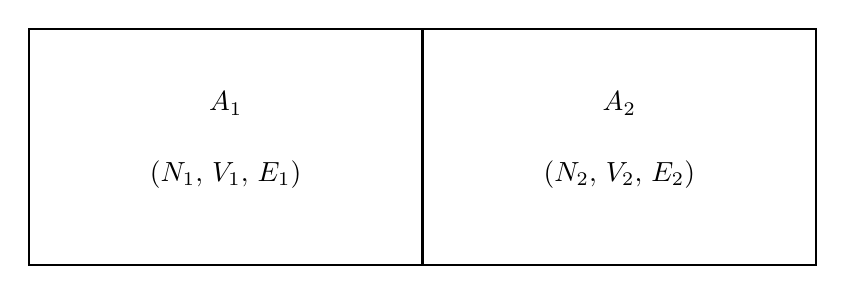
\begin{tikzpicture}[line width=0.8pt]
    % outer rectangle
    \draw (0,0) rectangle (10,3);
    % divider
    \draw (5,0) -- (5,3);

    % left block text
    \node at (2.5,2.05) {$A_{1}$};
    \node at (2.5,1.15) {$(N_{1},\,V_{1},\,E_{1})$};

    % right block text
    \node at (7.5,2.05) {$A_{2}$};
    \node at (7.5,1.15) {$(N_{2},\,V_{2},\,E_{2})$};
  \end{tikzpicture}
  \caption{示意两个系统 \(A_1(N_1,V_1,E_1)\) 与 \(A_2(N_2,V_2,E_2)\) 建立热接触。}
  \label{fig1.1}
\end{figure}



\(^{2}\)值得注意的是，\(\varepsilon_{i}\) 与 \(V\) 的依赖关系本身，是由系统的本质所决定的。例如，相对论系统与非相对论系统的情形并不相同；不妨对比一下第 1.4 节以及问题 1.7 中所讨论的两种情形。此外，我们还应注意到：原则上，\(\Omega\) 与 \(V\) 的依赖关系，源于这样一个事实：正是容器的物理尺寸，体现在对系统波函数施加的边界条件之中。
在此，\(E^{(0)}\) 表示复合系统 \(A^{(0)}\)（即 \(A_{1}+A_{2}\)）的能量；若 \(A_{1}\) 与 \(A_{2}\) 之间存在相互作用能量，则该相互作用能量将被忽略不计。在任意时刻 \(t\)，子系统 \(A_{1}\) 同样有概率处于 \(\Omega_{1}(E_{1})\) 的任一微观态中，而子系统 \(A_{2}\) 同样有概率处于 \(\Omega_{2}(E_{2})\) 的任一微观态中；因此，复合系统 \(A^{(0)}\) 同样有概率处于以下任一状态：
\begin{equation}\tag{1.2.4}\label{eq:1.2.4}
\Omega _ { 1 } ( E _ { 1 } ) \Omega _ { 2 } ( E _ { 2 } ) = \Omega _ { 1 } ( E _ { 1 } ) \Omega _ { 2 } ( E ^{( 0 )} - E _ { 1 } ) = \Omega ^{( 0 )} ( E ^{( 0 )} , E _ { 1 } )
\end{equation}
微观态。\(^{3}\) 显然，\(\Omega^{(0)}\) 本身会随 \(E_{1}\) 的变化而变化。现在的问题是：在何种 \(E_{1}\) 值下，复合系统将达到平衡？换句话说，能量交换需要达到多大程度，才能使子系统 \(A_{1}\) 和 \(A_{2}\) 达到相互平衡？
我们断言，这一过程将在 \(E_{1}\) 取得最大值时发生——即 \(\Omega^{(0)}(E^{(0)},E_{1})\) 的最大值所在处。其背后的哲学思想是：当一个物理系统被置于自然状态时，它会自然而然地朝向这样一种方向发展：通过不断增加微观态的数量，直至最终稳定于一个宏观态，而这个宏观态恰好拥有最多数量的微观态。从统计学的角度来看，我们认为，具有更多微观态的宏观态更为可能，而拥有最多微观态的宏观态则被视为最可能的状态。详细研究表明，对于典型的系统而言，任何偏离最可能宏观态的微观态数量，都比后者少上"数量级"之多。因此，系统的最可能状态，就是那个系统在其中度过"绝大多数"时间的宏观态。由此，将这一状态等同于系统的平衡状态，也就显得顺理成章。
我们将 \(E_{1}\) 的平衡值记作 \(\overline{E}_{1}\)（\(E_{2}\) 的平衡值记作 \(\overline{E}_{2}\)），在最大化 \(\Omega^{(0)}\) 时，我们得到：
\begin{equation}\tag{1.2.5}\label{eq:1.2.5}
\left( \frac { \partial \Omega _ { 1 } ( E _ { 1 } ) } { \partial E _ { 1 } } \right) _ { E _ { 1 } = \overline { { E } } _ { 1 } } \Omega _ { 2 } ( \overline { { E } } _ { 2 } ) + \Omega _ { 1 } ( \overline { { E } } _ { 1 } ) \left( \frac { \partial \Omega _ { 2 } ( E _ { 2 } ) } { \partial E _ { 2 } } \right) _ { E _ { 2 } = \overline { { E } } _ { 2 } } \cdot \frac { \partial E _ { 2 } } { \partial E _ { 1 } } = 0 .
\end{equation}
由于 \(\partial E_{2}/\partial E_{1}=-1\)，详见\autoref{eq:1.3.1}，上述条件可写为
\begin{equation}\tag{1.2.6}\label{eq:1.2.6}
\left( \frac { \partial \ln \Omega _ { 1 } ( E _ { 1 } ) } { \partial E _ { 1 } } \right) _ { E _ { 1 } = \overline { { E } } _ { 1 } } = \left( \frac { \partial \ln \Omega _ { 2 } ( E _ { 2 } ) } { \partial E _ { 2 } } \right) _ { E _ { 2 } = \overline { { E } } _ { 2 } } .
\end{equation}
因此，我们关于平衡状态的条件归结为子系统 \(A_{1}\) 和 \(A_{2}\) 分别的参数 \(\beta_{1}\) 和 \(\beta_{2}\) 的相等。其中，\(\beta\) 的定义如下：
\begin{equation}\tag{1.2.7}\label{eq:1.2.7}
\beta \equiv \left( \frac { \partial \ln \Omega ( N , V , E ) } { \partial E } \right) _ { N , V , E = \overline { { E } } } .
\end{equation}
³ 显而易见，复合系统 \(A^{(0)}\) 的宏观状态必须由两种能量来确定，即 \(E_{1}\) 和 \(E_{2}\)（否则，就只能是 \(E^{(0)}\) 与 \(E_{1}\)）。
因此，我们发现，当两个物理系统相互接触并实现能量交换时，这种能量交换会持续进行，直到变量 \(E_{1}\) 和 \(E_{2}\) 的平衡值 \(\overline{E}_{1}\) 和 \(\overline{E}_{2}\) 被达到。一旦这两个值被达到，两个系统之间便不再有净能量交换；此时，人们称这两个系统已达到热平衡状态。根据我们的分析，只有当参数 \(\beta\) 的相应值——即 \(\beta_{1}\) 和 \(\beta_{2}\)——相等时，这一过程才会发生。⁴ 因此，我们自然会预期，参数 \(\beta\) 与某一特定系统的热力学温度 \(T\) 存在某种关联。为了确定这一关系，我们回顾热力学公式
\begin{equation}\tag{1.2.8}\label{eq:1.2.8}
\left( \frac { \partial S } { \partial E } \right) _ { N , V } = \frac { 1 } { T } ,
\end{equation}
其中 \(S\) 为该系统的熵。将\autoref{eq:1.3.3} 与\autoref{eq:1.3.4} 进行比较，我们得出结论：热力学量 \(S\) 与统计量 \(\Omega\) 之间存在着密切的联系；事实上，对于任意一个物理系统，我们都可以写成
\begin{equation}\tag{1.2.9}\label{eq:1.2.9}
{ \frac { \Delta S } { \Delta ( \ln \Omega ) } } = { \frac { 1 } { \beta T } } = \mathrm { c o n s t . }
\end{equation}
这一对应关系最早由玻尔兹曼确立，他同时认为，由于热力学方法与统计学方法之间的关系似乎具有根本性，因此\autoref{eq:1.3.5} 中出现的常数必然是一个普遍常数。正是普朗克首次给出了明确的公式
\begin{equation}\tag{1.2.10}\label{eq:1.2.10}
S = k \ln \Omega ,
\end{equation}
不包含任何附加常数 \(S_0\)。目前，\autoref{eq:1.3.6} 以总微态数量为依据，根据给定的宏观状态，确定了某一特定物理系统的熵的绝对值。熵的零点则对应于一种特殊的状态，在这种状态下，仅有一个微态可被访问（\(\Omega=1\)）——即所谓的"唯一构型"；因此，统计学方法也为热力学第三定律提供了理论基础。\autoref{eq:1.3.6} 在物理学中具有至关重要的意义，它架起了微观世界与宏观世界之间的桥梁。
在热力学第二定律的研究中，我们了解到，熵增原理与这样一个事实密切相关：在宇宙的自然演化过程中，宇宙中的能量含量正日益减少，而可供转化为功的能量也越来越少；因此，某一特定系统的熵可以被视为衡量该系统中所普遍存在的"无序"或"混乱"的一种指标。公式（6）向我们揭示了无序是如何在微观层面产生的。显然，无序正是系统所能存在微态数量之多的体现。微态的选择越多，系统的可预测性就越低，从而导致系统中无序程度的升高。当系统完全处于有序状态时，
只有当系统别无选择，只能处于唯一一个状态（\(\Omega = 1\)）时，这一状态才对应于熵为零的状态。
根据公式（5）和（6），我们还得到
\begin{equation}\tag{1.2.11}\label{eq:1.2.11}
\beta = { \frac { 1 } { k T } } .
\end{equation}
普遍常数 \(k\) 通常被称为玻尔兹曼常数。在第1.4节中，我们将进一步探究 \(k\) 与气体常数 \(R\) 和阿伏伽德罗常数 \(N_{A}\) 之间的关系；详见公式（1.4.3）。\(^{5}\)
1.3 统计学与热力学的进一步联系
在延续前文的讨论之后，我们现在来探讨子系统 \(A_{1}\) 与 \(A_{2}\) 之间更为复杂的相互作用。若假设分隔两个子系统的壁既可移动又具有导电性，那么子系统 \(A_{1}\) 和 \(A_{2}\) 的各自体积 \(V_{1}\) 和 \(V_{2}\) 也会随之发生变化；事实上，总体积 \(V^{(0)}\)（即 \(V_{1}+V_{2}\)）保持不变，因此实际上我们只多出一个独立变量。当然，我们仍假定该壁对粒子完全不透，因此 \(N_{1}\) 和 \(N_{2}\) 的数值依然固定。按照先前的论证，当子系统 \(A^{(0)}\) 的状态熵 \(\Omega^{(0)}(V^{(0)},E^{(0)};V_{1},E_{1})\) 达到最大值时，复合系统 \(A^{(0)}\) 将达到平衡状态；也就是说，不仅
\begin{equation}\tag{1.3.1}\label{eq:1.3.1}
\left( \frac { \partial \ln \Omega _ { 1 } } { \partial E _ { 1 } } \right) _ { N _ { 1 } , V _ { 1 } ; \, E _ { 1 } = \overline { { E } } _ { 1 } } = \left( \frac { \partial \ln \Omega _ { 2 } } { \partial E _ { 2 } } \right) _ { N _ { 2 } , V _ { 2 } ; \, E _ { 2 } = \overline { { E } } _ { 2 } } ,
\end{equation}
而且
\begin{equation}\tag{1.3.2}\label{eq:1.3.2}
\left( \frac { \partial \ln \Omega _ { 1 } } { \partial V _ { 1 } } \right) _ { N _ { 1 } , E _ { 1 } ; \; V _ { 1 } = \overline { { V } } _ { 1 } } = \left( \frac { \partial \ln \Omega _ { 2 } } { \partial V _ { 2 } } \right) _ { N _ { 2 } , E _ { 2 } ; \; V _ { 2 } = \overline { { V } } _ { 2 } } .
\end{equation}
我们关于平衡状态的条件现在表现为：子系统 \(A_{1}\) 的参数对 \((\beta_{1},\eta_{1})\) 与子系统 \(A_{2}\) 的参数对 \((\beta_{2},\eta_{2})\) 之间满足等式，而根据定义，
\begin{equation}\tag{1.3.3}\label{eq:1.3.3}
\eta \equiv \left( \frac { \partial \ln \Omega ( N , V , E ) } { \partial V } \right) _ { N , E , V = \overline { { V } } } .
\end{equation}
同样地，如果 \(A_{1}\) 和 \(A_{2}\) 通过一堵允许粒子交换的壁彼此接触，那么平衡状态的条件还将因以下等式而进一步加强：
子系统 \(A_{1}\) 的参数 \(\zeta_{1}\) 与子系统 \(A_{2}\) 的参数 \(\zeta_{2}\) 之间也满足等式，而根据定义，
\begin{equation}\tag{1.3.4}\label{eq:1.3.4}
\zeta \equiv \left( \frac { \partial \ln \Omega ( N , V , E ) } { \partial N } \right) _ { V , E , N = \overline { { { N } } } } .
\end{equation}
为了确定参数 \(\eta\) 和 \(\zeta\) 的物理意义，我们借助\autoref{eq:1.2.6} 以及热力学的基本公式，即
\begin{equation}\tag{1.3.5}\label{eq:1.3.5}
d E = T \, d S - P \, d V + \mu \, d N ,
\end{equation}
其中 \(P\) 为热力学压力，\(\mu\) 为给定体系的化学势。由此可得
\begin{equation}\tag{1.3.6}\label{eq:1.3.6}
\eta = \frac { P } { k T }  \mathrm { a n d }  \zeta = - \frac { \mu } { k T } .
\end{equation}
从物理角度来看，这些结果完全令人满意，因为在热力学意义上，当两个系统 \(A_{1}\) 和 \(A_{2}\) 之间处于平衡状态时，若将二者隔开的壁既具有导电性又可移动（从而使其各自的能量和体积发生变化），那么其条件与\autoref{eq:1.3.1} 和 \autoref{eq:1.3.1} 中所包含的条件实际上完全一致，即
\begin{equation}\tag{1.3.7}\label{eq:1.3.7}
T _ { 1 } = T _ { 2 }  \mathrm { a n d }  P _ { 1 } = P _ { 2 } .
\end{equation}
另一方面，如果这两个系统既能交换粒子，又能交换能量，但其体积保持固定，那么在热力学上所获得的平衡条件，确实为
\begin{equation}\tag{1.3.8}\label{eq:1.3.8}
T _ { 1 } = T _ { 2 }  \mathrm { a n d }  \mu _ { 1 } = \mu _ { 2 } .
\end{equation}
最后，若交换过程使得这三种（宏观）参数均变为可变，则平衡条件将变为
\begin{equation}\tag{1.3.9}\label{eq:1.3.9}
T _ { 1 } = T _ { 2 } ,  P _ { 1 } = P _ { 2 } ,  \mathrm { a n d }  \mu _ { 1 } = \mu _ { 2 } .
\end{equation}
令人欣慰的是，这些结论与基于统计学考量所得出的结果完全一致。
结合前述讨论的结果，我们得出以下从统计学出发推导热力学的法则：对于给定系统的宏观态 \((N,V,E)\)，确定该系统所能达到的所有可能微观态的数量；将这一数量称为 \(\Omega(N,V,E)\)。随后，该状态下系统的熵可由
基本公式
\begin{equation}\tag{1.3.10}\label{eq:1.3.10}
S ( N , V , E ) = k \ln \Omega ( N , V , E ) ,
\end{equation}
而主导的强度场——即温度、压力和化学势——则由
\begin{equation}\tag{1.3.11}\label{eq:1.3.11}
\left( \frac { \partial S } { \partial E } \right) _ { N , V } = \frac { 1 } { T } ;  \left( \frac { \partial S } { \partial V } \right) _ { N , E } = \frac { P } { T } ;  \left( \frac { \partial S } { \partial N } \right) _ { V , E } = - \frac { \mu } { T } .
\end{equation}
或者，我们也可以写成
\begin{equation}\tag{1.3.12}\label{eq:1.3.12}
P = \left( \frac { \partial S } { \partial V } \right) _ { N , E } \Bigg / \left( \frac { \partial S } { \partial E } \right) _ { N , V } = - \left( \frac { \partial E } { \partial V } \right) _ { N , S }
\end{equation}
以及
\begin{equation}\tag{1.3.13}\label{eq:1.3.13}
\mu = - \left( \frac { \partial S } { \partial N } \right) _ { V , E } \bigg / \left( \frac { \partial S } { \partial E } \right) _ { N , V } = \left( \frac { \partial E } { \partial N } \right) _ { V , S } ,
\end{equation}
同时，
\begin{equation}\tag{1.3.14}\label{eq:1.3.14}
T = \left( { \frac { \partial E } { \partial S } } \right) _ { N , V } .
\end{equation}
\autoref{eq:1.3.11} 至 \autoref{eq:1.3.13} 也同样可以由\autoref{eq:1.3.4} 得到。事实上，要根据这些公式计算 \(P\)、\(\mu\) 和 \(T\)，必须将能量 \(E\) 表示为 \(N\)、\(V\) 和 \(S\) 的函数；原则上，一旦 \(S\) 被知悉为 \(N\)、\(V\) 和 \(E\) 的函数，这一操作便应成为可能。
其余的热力学内容则可轻松推导出来；请参阅附录 H。例如，亥姆霍兹自由能 \(A\)、吉布斯自由能 \(G\) 以及焓 \(H\) 分别由
\begin{equation}\tag{1.3.15}\label{eq:1.3.15}
\begin{array}{rl} & { A = E - T S , } \\& { G = A + P V = E - T S + P V } \\& { = \mu N } \end{array}
\end{equation}
\(^{7}\)在撰写这些公式时，我们运用了偏微分学中广为人知的关系，即"若三个变量 \(x\)、\(y\) 和 \(z\) 之间存在相互关系，则（参见附录 H）
\begin{equation}\tag{1.3.16}\label{eq:1.3.16}
\left(\frac{\partial x}{\partial y}\right)_z\left(\frac{\partial y}{\partial z}\right)_x\left(\frac{\partial z}{\partial x}\right)_y=-1."
\end{equation}
\(^{8}\)关系 \(E-TS+PV=\mu N\) 可以直接从式（4）中推导出来。为此，我们只需将所给系统视为在渐进的过程中逐渐扩展至当前尺寸，使得在这一过程中，各组分参数 \(T\)、\(P\) 和 \(\mu\) 保持恒定，而广延参数 \(N\)、\(V\) 和 \(E\)（以及由此产生的 \(S\)）则彼此按比例相应地增长。
并且
\begin{equation}\tag{1.3.17}\label{eq:1.3.17}
H = E + P V = G + T S .
\end{equation}
定容热容 \(C_{V}\) 与定压热容 \(C_{P}\) 分别为：
\begin{equation}\tag{1.3.18}\label{eq:1.3.18}
C _ { V } \equiv T \left( \frac { \partial S } { \partial T } \right) _ { N , V } = \left( \frac { \partial E } { \partial T } \right) _ { N , V }
\end{equation}
并且
\begin{equation}\tag{1.3.19}\label{eq:1.3.19}
C _ { P } \equiv T \left( \frac { \partial S } { \partial T } \right) _ { N , P } = \left( \frac { \partial ( E + P V ) } { \partial T } \right) _ { N , P } = \left( \frac { \partial H } { \partial T } \right) _ { N , P } .
\end{equation}
\section{经典理想气体}\label{ux7ecfux5178ux7406ux60f3ux6c14ux4f53}
为了说明前几节所阐述的分析方法，我们现在将推导出由单原子分子构成的经典理想气体的各项热力学性质。我们之所以选择这一高度专业化的体系进行研究，主要是因为它能够对数 \(\Omega(N,V,E)\) 进行明确且近乎渐近式的计算。当我们发现通过研究这一体系，我们可以以最直观的方式，借助其他物理常数来确定玻尔兹曼常数 \(k\)——详见式（3）——这一事实更加凸显了其重要性。此外，该体系的行为也为研究其他物理系统提供了有益的参考依据，尤其是那些真实气体（无论是否受到量子效应的影响）。事实上，在高温低密度的极限条件下，理想气体的行为便成为大多数真实系统的典型行为。
在对这一案例展开详细研究之前，有必要先指出一点，这一点适用于所有由非相互作用粒子构成的经典系统，无论这些粒子的内部结构如何。这一要点与数 \(\Omega(N,V,E)\) 对 \(V\) 的显式依赖性有关，进而也与这些系统的状态方程息息相关。如果粒子之间不存在任何空间上的相关性，也就是说，任何一个粒子出现在可用空间特定区域的概率完全独立于其他粒子的位置，那么 \(N\) 个粒子在系统中进行空间分布的总方式数，将仅仅等于各个粒子在各自独立的空间中占据位置的方式数的乘积。在 \(N\) 和 \(E\) 固定的情况下，这两个数值将与容器的体积 \(V\) 成正比；相应地，总方式数也将与 \(V\) 的 \(N\) 次方成正比：
\begin{equation}\tag{1.3.20}\label{eq:1.3.20}
\Omega ( N , E , V ) \propto V ^{N} .
\end{equation}
若满足以下两个条件，则上述结论成立：（1）粒子之间的相互作用可以忽略不计；（2）单个粒子的波包不会发生显著重叠——换言之，量子效应同样可以忽略不计。
结合方程（1.3.9）和（1.3.10），我们得到
\begin{equation}\tag{1.3.21}\label{eq:1.3.21}
\frac { P } { T } = k \left( \frac { \partial \ln \Omega ( N , E , V ) } { \partial V } \right) _ { N , E } = k \frac { N } { V } .
\end{equation}
若系统中包含 \(n\) 摩尔的气体，则 \(N = nN_A\)，其中 \(N_A\) 是阿伏伽德罗常数。于是，方程（2）变为
\begin{equation}\tag{1.3.22}\label{eq:1.3.22}
P V = N k T = n R T  ( R = k N _ { A } ) ,
\end{equation}
这就是著名的理想气体状态方程，其中 \(R\) 为每摩尔气体的气体常数。因此，对于任何由非相互作用粒子组成的经典系统而言，理想气体状态方程均适用。
要推导该系统的其他热力学性质，我们需要深入了解 \(\Omega\) 如何依赖于参数 \(N\)、\(V\) 和 \(E\)。问题本质上归结为：确定方程（1.1.1）和（1.1.2）同时满足的总方式数。换句话说，我们必须计算出满足方程的总方式数（即独立的方式数）。
\begin{equation}\tag{1.3.23}\label{eq:1.3.23}
\sum _ { r = 1 } ^{3 N} \varepsilon _ { r } = E ,
\end{equation}
其中 \(\varepsilon_{r}\) 分别对应 \(N\) 个粒子各自由度所对应的能量。之所以这一数值需要依赖于参数 \(N\) 和 \(E\)，原因十分显而易见。然而，这一数值同样取决于变量 \(\varepsilon_{r}\) 可取的"值域"；正是通过这一值域，才产生了对 \(V\) 的依赖关系。现在，对于一个自由的、非相对论性粒子，其能量本应满足以下条件：该粒子被限制在边长为 \(L\) 的立方体盒中（\(V=L^{3}\)），且波函数 \(\psi(\boldsymbol{r})\) 在边界上处处为零。此时，该粒子的能量本应满足以下公式：
\begin{equation}\tag{1.3.24}\label{eq:1.3.24}
\varepsilon ( n _ { x } , n _ { y } , n _ { z } ) = \frac { h ^{2} } { 8 m L ^{2} } ( n _ { x } ^{2} + n _ { y } ^{2} + n _ { z } ^{2} ) ;  n _ { x } , n _ { y } , n _ { z } = 1 , 2 , 3 , \ldots ,
\end{equation}
其中 \(h\) 是普朗克常数，\(m\) 是粒子的质量。因此，对于能量为 \(\varepsilon\) 的粒子，其不同的本征函数（或微态）的数量，将等于方程
\begin{equation}\tag{1.3.25}\label{eq:1.3.25}
\left( n _ { x } ^{2} + n _ { y } ^{2} + n _ { z } ^{2} \right) = \frac { 8 m V ^{2 / 3} \varepsilon } { \hbar ^{2} } = \varepsilon ^{*} .
\end{equation}
我们可以将这一数量记作 \(\Omega(1,\varepsilon,V)\)。进一步推演可知，所求的总数 \(\Omega(N,E,V)\) 将等于方程
\begin{equation}\tag{1.3.26}\label{eq:1.3.26}
\sum _ { r = 1 } ^{3 N} n _ { r } ^{2} = \frac { 8 m V ^{2 / 3} E } { h ^{2} } = E ^{*} ,  \mathrm { s a y } .
\end{equation}
从方程（7）中可直接得出一个重要结论，甚至在明确计算出 \(\Omega(N,E,V)\) 之前即可得出。根据该方程右侧表达式的本质，我们推断：系统的体积 \(V\) 和能量 \(E\) 以 \((V^{2/3}E)\) 这一组合的形式，纳入了 \(\Omega\) 的表达式之中。因此，
\begin{equation}\tag{1.3.27}\label{eq:1.3.27}
S ( N , V , E ) \equiv S \Bigl ( N , V ^{2 / 3} E \Bigr ) .
\end{equation}
由此可见，为了使 \(S\) 和 \(N\) 保持恒定，从而定义一个可逆绝热过程，
\begin{equation}\tag{1.3.28}\label{eq:1.3.28}
V ^{2 / 3} E = \mathrm { c o n s t . }
\end{equation}
方程（1.3.11）由此得出
\begin{equation}\tag{1.3.29}\label{eq:1.3.29}
P = - \left( { \frac { \partial E } { \partial V } } \right) _ { N , S } = { \frac { 2 } { 3 } } { \frac { E } { V } } ,
\end{equation}
也就是说，非相对论性、非相互作用粒子系统的压力恰好等于其能量密度的三分之二。\(^{10}\) 值得注意的是，由于尚未对数 \(\Omega\) 进行明确的计算，因此结果（9）和（10）既适用于量子统计，也适用于经典统计；将这两者结合起来所得的结果同样具有普遍性，即
\begin{equation}\tag{1.3.30}\label{eq:1.3.30}
P V ^{5 / 3} = \mathrm { c o n s t . } ,
\end{equation}
这告诉我们，在可逆绝热过程中，\(P\) 如何随 \(V\) 变化。
接下来，我们将尝试对数 \(\Omega\) 进行求值。在这一求值过程中，我们明确假设粒子是可区分的，因此，如果状态 \(i\) 中的某个粒子与状态 \(j\) 中的某个粒子发生互换，则所得到的微观状态将被计为不同的状态。因此，数 \(\Omega(N,V,E)\)，或者更准确地说，\(\Omega_{N}(E^{*})\)（参见式（7）），等于位于一个 \(3N\) 维球面上、半径为 \(\sqrt{E^{*}}\) 的正整数点的数量。显然，这个数会随着 \(E^{*}\) 的变化呈现出极其不规则的特性：对于两个给定的 \(E^{*}\) 值，尽管它们可能彼此非常接近，但该数的取值却可能大相径庭。相比之下，数 \(\Sigma_{N}(E^{*})\)——即位于或位于以 \(\sqrt{E^{*}}\) 为半径的 \(3N\) 维球面表面或其内部的正整数点数量——则要不那么不规则。就我们的物理问题而言，这相当于系统中微态的数量 \(\Sigma(N,V,E)\)，即在满足所有由参数 \(N\) 和 \(V\) 确定的宏观状态的前提下，且能量低于
大于或等于 \(E\)；也就是说，
\begin{equation}\tag{1.3.31}\label{eq:1.3.31}
\Sigma ( N , V , E ) = \sum _ { E ^{\prime} \leq E } \Omega ( N , V , E ^{\prime} )
\end{equation}
或者
\begin{equation}\tag{1.3.32}\label{eq:1.3.32}
\sum _ { N } ( E ^{*} ) = \sum _ { E ^{* ^ { \prime} } \leq E ^{*} } \Omega _ { N } ( E ^{* ^ { \prime} } ) .
\end{equation}
当然，数 \(\Sigma\) 也会存在一定程度的不规则性；然而，我们预期，当 \(E^{*} \rightarrow \infty\) 时，它的渐近行为将比 \(\Omega\) 的渐近行为平滑得多。在后续的讨论中，我们将看到，该系统的热力学性质，无论是从数 \(\Sigma\) 还是从数 \(\Omega\) 得到的，都同样能够很好地描述。
要理解此处所阐述的观点，不妨稍作离题，深入探讨数值 \(\Omega_{1}(\varepsilon^{*})\) 和 \(\Sigma_{1}(\varepsilon^{*})\) 的行为——这两者对应于单个粒子被限制在给定体积 \(V\) 中的情形。对于 \(\varepsilon^{*} \leq 10,000\)，这些数值的精确取值可从古普塔（1947）编撰的表格中获得。数值 \(\Omega_{1}(\varepsilon^{*})\) 那些剧烈而不规则的变化几乎难以忽视。相比之下，数值 \(\Sigma_{1}(\varepsilon^{*})\) 则呈现出更为平滑的渐近行为。从问题的几何结构出发，我们注意到：在渐近意义上，\(\Sigma_{1}(\varepsilon^{*})\) 应当等于一个半径为 \(\sqrt{\varepsilon^{*}}\) 的三维球体中一个八分之一象限的体积，即，
\begin{equation}\tag{1.3.33}\label{eq:1.3.33}
\operatorname* { l i m } _ { \varepsilon ^{*} \to \infty } { \frac { \sum _ { 1 } ( \varepsilon ^{*} ) } { ( \pi / 6 ) \varepsilon ^{* 3 / 2} } } = 1 .
\end{equation}
更细致的分析表明，按照下一次近似计算（参见帕特里亚，1966），
\begin{equation}\tag{1.3.34}\label{eq:1.3.34}
\Sigma _ { 1 } ( \varepsilon ^{*} ) \approx \frac { \pi } { 6 } \varepsilon ^{* 3 / 2} - \frac { 3 \pi } { 8 } \varepsilon ^{*} ;
\end{equation}
修正项的产生源于这样一个事实：八分之一象限的体积在一定程度上高估了所需晶格点的数量，因为它在某种程度上包含了那些某个或多个坐标为零的点。图~1.2展示了 \(\varepsilon^{*}\) 介于200至300之间的 \(\Sigma_{1}(\varepsilon^{*})\) 实际数值的直方图；同时，也展示了理论估算值（15）。在图中，我们还加入了相应微态数量 \(\Sigma_{1}^{\prime}(\varepsilon^{*})\) 的实际数值直方图——当量子数 \(n_{x}\)、\(n_{y}\) 和 \(n_{z}\) 均可取零值时的情况。在后一种情况下，八分之一象限的体积在一定程度上低估了所需晶格点的数量；如今，我们得到了
\begin{equation}\tag{1.3.35}\label{eq:1.3.35}
\Sigma _ { 1 } ^{\prime} ( \varepsilon ^{*} ) \approx \frac { \pi } { 6 } \varepsilon ^{* 3 / 2} + \frac { 3 \pi } { 8 } \varepsilon ^{*} .
\end{equation}
然而，在渐近意义上，数值 \(\Sigma_{1}^{\prime}(\varepsilon^{*})\) 也满足方程（14）。
回到 \(N\) 个粒子的问题，数值 \(\Sigma_{N}(E^{*})\) 在渐近意义上应等于一个 \(3N\) 维球体中"正向区域"的"体积"。
对数运算并应用斯特林公式（附录~B中的方程B.29），
\begin{equation}\tag{1.3.36}\label{eq:1.3.36}
\ln ( n ! ) \approx n \ln n - n  ( n \gg 1 ) ,
\end{equation}
我们得到
\begin{equation}\tag{1.3.37}\label{eq:1.3.37}
\ln \Sigma ( N , V , E ) \approx N \ln \left[ \frac { V } { h ^{3} } \left( \frac { 4 \pi m E } { 3 N } \right) ^{3 / 2} \right] + \frac { 3 } { 2 } N .
\end{equation}
要推导所给系统的热力学性质，我们不得不以某种方式确定系统的能量的精确值，或为其设定一个限定范围。鉴于函数 \(\Omega(N,V,E)\) 的特性极其不规则，从物理角度而言，无法为系统的能量赋予一个确切的数值，因为这样无论如何都无法得到系统热力学函数的光滑、连续的表达式。从实际应用的角度来看，完全孤立的系统也过于理想化。在现实世界中，几乎每一个系统都会与周围环境存在一定的相互作用，哪怕这种相互作用微乎其微；因此，系统的能量无法被精确地界定。¹² 当然，能量变化范围的实际宽度，与能量的平均值相比，通常都相当小。我们不妨将这一范围限定为 \(E - \frac{1}{2}\Delta\) 和 \(E + \frac{1}{2}\Delta\) 两个极限值——假设 \(\Delta \ll E\)；通常情况下，\(\Delta/E = O(1/\sqrt{N})\)。相应地，系统的微观状态数 \(\Gamma(N,V,E;\Delta)\) 可以表示为：
\begin{equation}\tag{1.3.38}\label{eq:1.3.38}
\Gamma ( N , V , E ; \Delta ) \simeq \frac { \partial \Sigma ( N , V , E ) } { \partial E } \Delta \approx \frac { 3 N } { 2 } \frac { \Delta } { E } \Sigma ( N , V , E ) ,
\end{equation}
由此可得
\begin{equation}\tag{1.3.39}\label{eq:1.3.39}
\ln \Gamma ( N , V , E ; \Delta ) \approx N \ln \left[ \frac { V } { \hbar ^{3} } \left( \frac { 4 \pi m E } { 3 N } \right) ^{3 / 2} \right] + \frac { 3 } { 2 } N + \left\{ \ln \left( \frac { 3 N } { 2 } \right) + \ln \left( \frac { \Delta } { E } \right) \right\} .
\end{equation}
现在，当 \(N \gg 1\) 时，花括号中的第一项与括号外的任何项相比都可忽略不计，因为 \(\lim_{N \to \infty} (\ln N)/N = 0\)。此外，对于任意合理的 \(\Delta/E\) 值，花括号中的第二项也同样如此。¹³ 因此，在实际应用中，
\begin{equation}\tag{1.3.40}\label{eq:1.3.40}
\ln \Gamma \approx \ln \Sigma \approx \mathcal { N } \ln \left[ \frac { V } { \hbar ^{3} } \left( \frac { 4 \pi m E } { 3 N } \right) ^{3 / 2} \right] + \frac { 3 } { 2 } N .
\end{equation}
于是，我们得到了一个令人费解的结果：在实际应用中，系统能量允许变化的范围实际上差异不大；能量可能介于 \(E - \frac{1}{2}\Delta\) 与 \(E + \frac{1}{2}\Delta\) 之间，或者同样可以是 0 与 \(E\) 之间。造成这一现象的原因在于，系统微观状态数的增长速率
随着能量的增加而呈指数级增长，这一点在式（1.4.17） 中已有充分说明；即使我们允许能量取任意介于 0 与某一特定值 \(E\) 之间的数值，真正对这一数量贡献最大的，也仅仅是 \(E\) 的"近邻区域"！而且，由于我们最终只关心这一数量的对数，因此即便只是该"近邻区域"的"宽度"，也已不再具有重要意义！
如今，我们已经为推导系统的热力学性质做好了充分准备。首先，我们有
\begin{equation}\tag{1.3.41}\label{eq:1.3.41}
S ( N , V , E ) = k \ln \Gamma = N k \ln \left[ \frac { V } { \hbar ^{3} } \left( \frac { 4 \pi \, m E } { 3 N } \right) ^{3 / 2} \right] + \frac { 3 } { 2 } N k ,
\end{equation}
该式可逆代换，从而得到
\begin{equation}\tag{1.3.42}\label{eq:1.3.42}
E ( S , V , N ) = \frac { 3 h ^{2} N } { 4 \pi m V ^{2 / 3} } \exp \left( \frac { 2 S } { 3 N k } - 1 \right) .
\end{equation}
随后，借助\autoref{eq:1.3.10} 或 \autoref{eq:1.3.13}，即可求得气体的温度，并由此得出能量与温度的关系式
\begin{equation}\tag{1.3.43}\label{eq:1.3.43}
E = N \bigg ( \frac { 3 } { 2 } k T \bigg ) = n \bigg ( \frac { 3 } { 2 } R T \bigg ) ,
\end{equation}
其中，\(n\) 为气体的摩尔数。借助公式（1.3.17），可得恒容热容：
\begin{equation}\tag{1.3.44}\label{eq:1.3.44}
C _ { V } = \left( \frac { \partial E } { \partial T } \right) _ { N , V } = \frac { 3 } { 2 } N k = \frac { 3 } { 2 } n R .
\end{equation}
对于状态方程，我们得到
\begin{equation}\tag{1.3.45}\label{eq:1.3.45}
P = - \left( \frac { \partial E } { \partial V } \right) _ { N , S } = \frac { 2 } { 3 } \frac { E } { V } ,
\end{equation}
这一结果与我们先前得出的结论（10）一致。结合（23），我们得到
\begin{equation}\tag{1.3.46}\label{eq:1.3.46}
P = { \frac { N k T } { V } }  { \mathrm { o r } }  P V = n R T ,
\end{equation}
这与（3）完全相同。恒压热容由下式给出，参见（1.3.18）：
\begin{equation}\tag{1.3.47}\label{eq:1.3.47}
C _ { P } = \left( \frac { \partial ( E + P V ) } { \partial T } \right) _ { N , P } = \frac { 5 } { 2 } n R ,
\end{equation}
因此，今后我们将用等号代替"≈"这一表示关系渐近特性的符号，因为在大多数物理系统中，渐近结果几乎可以达到精确结果。
因此，对于两种比热之比，我们有
\begin{equation}\tag{1.3.48}\label{eq:1.3.48}
\gamma = C _ { P } / C _ { V } = \frac { 5 } { 3 } .
\end{equation}
现在，假设气体经历了一次等温状态变化（\(T=\mathrm{常数}\)，\(N=\mathrm{常数}\)）；根据（23），气体的总能量将保持不变；而根据（26），其压力会随体积呈反比变化（波义耳定律）。在初始状态 \(i\) 和最终状态 \(f\) 之间，气体熵的变化量则为，参见式（21），
\begin{equation}\tag{1.3.49}\label{eq:1.3.49}
S _ { f } - S _ { i } = N k \ln ( V _ { f } / V _ { i } ) .
\end{equation}
另一方面，如果气体经历了一次可逆绝热状态变化（\(S=\mathrm{常数}\)，\(N=\mathrm{常数}\)），则根据（22）和（23），\(E\) 和 \(T\) 都会随体积呈 \(V^{-2/3}\) 的变化；因此，根据（25）或（26），\(P\) 会随体积呈 \(V^{-5/3}\) 的变化。这些结果与传统的热力学规律相符，即
\begin{equation}\tag{1.3.50}\label{eq:1.3.50}
P V ^{\gamma} = \mathrm { c o n s t . }  \mathrm { a n d }  T V ^{\gamma - 1} = \mathrm { c o n s t . } ,
\end{equation}
其中 \(\gamma=\frac{5}{3}\)。值得注意的是，在热力学上，绝热过程中 \(E\) 的变化仅源于气体对周围环境所做的外力功，反之亦然：
\begin{equation}\tag{1.3.51}\label{eq:1.3.51}
( d E ) _ { \mathrm { a d i a b } } = - P d V = - \frac { 2 E } { 3 V } d V ;
\end{equation}
参见式（1.3.4）和（25）。\(E\) 与 \(V\) 的依赖关系可从这一关系中轻松推导出来。
本节的讨论清晰地表明，宏观系统的热力学可以从其微观状态的多重性（以数值 \(\Omega\)、\(\Gamma\) 或 \(\Sigma\) 表示）中推导出来。整个问题的关键在于对这些数值进行渐近计数，然而遗憾的是，这一任务仅在少数理想化情形下才得以解决，例如本节所探讨的情形；另请参阅问题 1.7 和 1.8。即便是在这样理想化的案例中，仍然存在一种不足之处——这种不足在迄今为止的推导过程中并未被察觉；这一不足与 S 对 \(N\) 的显式依赖性有关。下一节的讨论不仅旨在揭示这一不足，还旨在为此提供必要的补救措施。
\section{混合熵与吉布斯悖论}\label{ux6df7ux5408ux71b5ux4e0eux5409ux5e03ux65afux6096ux8bba}
从表达式（1.4.21）中我们很容易注意到的一点是，与逻辑上所期望的情况相反，根据该表达式给出的理想气体的熵，并不是广延量。
（N 1 , V 1 ; T）
（N 2 , V 2 ; T）
系统的属性！也就是说，如果我们把系统规模放大一个因子 \(\alpha\)，同时保持其各组分的强度变量不变，那么本应随之也放大相同因子 \(\alpha\) 的系统熵却并未按此比例增长；表达式中 \(\ln V\) 项的存在，对结果产生了不利影响。从某种意义上说，这表明该系统的熵与其各部分熵之和并不一致，而这种情形在物理上是完全不合理的。更常见的处理方式是考虑所谓的吉布斯悖论。
吉布斯将两种理想气体 1 和 2 混合的过程可视化——这两种气体最初都处于相同的温度 \(T\)；参见图~1.3。显然，混合后的温度也应为同一温度。然而，在混合发生之前，两种气体各自的熵分别为，如式（1.4.21）和式（1.4.23）所示，
\begin{equation}\tag{1.3.52}\label{eq:1.3.52}
S _ { i } = N _ { i } k \ln V _ { i } + \frac { 3 } { 2 } N _ { i } k \left\{ 1 + \ln \left( \frac { 2 \pi m _ { i } k T } { h ^{2} } \right) \right\} ;  i = 1 , 2 .
\end{equation}
当混合过程完成后，总熵将为
\begin{equation}\tag{1.3.53}\label{eq:1.3.53}
S _ { T } = \sum _ { i = 1 } ^{2} \left[ N _ { i } k \ln V + \frac { 3 } { 2 } N _ { i } k \left\{ 1 + \ln \left( \frac { 2 \pi m _ { i } k T } { h ^{2} } \right) \right\} \right] ,
\end{equation}
其中 \(V = V_1 + V_2\)。因此，\(S\) 值的净增加量——即所谓"混合熵"——可表示为
\begin{equation}\tag{1.3.54}\label{eq:1.3.54}
( \Delta S ) = S _ { T } - \sum _ { i = 1 } ^{2} S _ { i } = k \left[ N _ { 1 } \ln { \frac { V _ { 1 } + V _ { 2 } } { V _ { 1 } } } + N _ { 2 } \ln { \frac { V _ { 1 } + V _ { 2 } } { V _ { 2 } } } \right] ;
\end{equation}
\(\Delta S\) 这一量确实为正，因为在像混合这样不可逆的过程中，这一量理应为正。现在，若两种气体的初始粒子密度（从而混合物的粒子密度）也相同，则式（3）变为
\begin{equation}\tag{1.3.55}\label{eq:1.3.55}
( \Delta S ) ^{*} = k \Bigg [ N _ { 1 } \ln \frac { N _ { 1 } + N _ { 2 } } { N _ { 1 } } + N _ { 2 } \ln \frac { N _ { 1 } + N _ { 2 } } { N _ { 2 } } \Bigg ] ,
\end{equation}
这一结果同样为正。
\^{}\{15\}这意味着将参数 \(N\)、\(V\) 和 \(E\) 分别提升至 \(\alpha N\)、\(\alpha V\) 和 \(\alpha E\)，从而使每粒子的能量和每粒子的体积保持不变。
到目前为止，一切似乎都还正常。然而，如果我们将两种相同气体的样品进行混合，就会出现一种矛盾的现象。再次强调，各独立样品的熵将由式（1）给出；当然，此时 \(m_{1}=m_{2}=m\)，例如。而混合后的熵则由以下公式给出：
\begin{equation}\tag{1.3.56}\label{eq:1.3.56}
S _ { T } = N k \ln V + \frac { 3 } { 2 } N k \left\{ 1 + \ln \left( \frac { 2 \pi \, m k T } { h ^{2} } \right) \right\} ,
\end{equation}
其中 \(N = N_{1} + N_{2}\)；需要注意的是，该表达式在数值上与式（2）完全相同，且 \(m_{i} = m\)。因此，在这种情况下，混合熵同样可由式（3）给出；若 \(N_{1}/V_{1} = N_{2}/V_{2} = (N_{1} + N_{2})/(V_{1} + V_{2})\)，则可由式（4）给出。然而，最后这一结论并不成立，因为将两种相同气体的样品混合在一起——其初始温度均为 \(T\)，初始粒子密度均为 \(n\)——显然是一个可逆过程。因为我们只需将分隔壁重新插入系统中，便能得到一种与混合前完全相同的状态。当然，我们在此暗含地认为，在处理由相同粒子组成的系统时，我们无法对它们逐一进行追踪；我们所能依据的，仅仅是它们的数量。当两种不相容的气体混合在一起时，即便它们的初始温度均为 \(T\)，初始粒子密度均为 \(n\)，这一过程却属于不可逆过程；因为一旦重新插入分隔壁，我们就会得到两种混合物的样品，而非原本存在的两种气体。对于这种情况，式（4）确实适用。然而，在本例中，相应的结果应当是
\begin{equation}\tag{1.3.57}\label{eq:1.3.57}
( \Delta S ) _ { 1 = 2 } ^{*} = 0 .
\end{equation}
上述结果也与这样一条要求一致：某一系统的熵等于其各部分熵之和。当然，我们早已注意到，式（1.4.21）并不能保证这一点。因此，我们再次不得不相信，该式本身存在根本性的问题。
要理解如何避免上述矛盾的局面，我们不妨回想一下：对于两种相同气体的样品混合过程，若其初始温度均为 \(T\)，初始粒子密度均为 \(n\)，我们曾得出结果（4），该结果也可以写成：
\begin{equation}\tag{1.3.58}\label{eq:1.3.58}
( \Delta S ) ^{*} = S _ { T } - ( S _ { 1 } + S _ { 2 } ) \approx k [ \ln \{ ( N _ { 1 } + N _ { 2 } ) ! \} - \ln ( N _ { 1 } ! ) - \ln ( N _ { 2 } ! ) ] ,
\end{equation}
与其采用逻辑上的结果（4a），我们不妨仔细审视这一表达式。会发现，如果我们将 \(S\) 的原始表达式减去一个特设项——\(k\ln(N!)\)——那么我们确实能够得到正确的结果。因为这将使 \(S_1\) 减少 \(k\ln(N_1!)\)，\(S_2\) 减少 \(k\ln(N_2!)\)，而 \(S_T\) 则减少 \(k\ln\{(N_1+N_2)!\}\)，最终使得 \((\Delta S)^*\) 为零，而不是式（4）中所呈现的结果。显然，这实际上相当于将统计量 \(\Gamma\) 和 \(\Sigma\) 以 \(N!\) 为因子进行了调整。而这正是吉布斯所提出的解决该悖论的方案。
如果我们同意上述建议，那么经典理想气体的熵修正表达式将变为：
\begin{equation}\tag{1.3.59}\label{eq:1.3.59}
\begin{array}{rl} & { S ( N , V , E ) = N k \ln \left[ \frac { V } { N h ^{3} } \left( \frac { 4 \pi \, m E } { 3 N } \right) ^{3 / 2} \right] + \frac { 5 } { 2 } N k } \\& {  = N k \ln \left( \frac { V } { N } \right) + \frac { 3 } { 2 } N k \left\{ \frac { 5 } { 3 } + \ln \left( \frac { 2 \pi \, m k T } { h ^{2} } \right) \right\} , } \end{array}
\end{equation}
这的确是一种真正广义的表达式！若我们现在将两种相同气体的样品混合在一起，且其初始温度均为 \(T\)，那么混合熵将为：
\begin{equation}\tag{1.3.60}\label{eq:1.3.60}
( \Delta S ) _ { 1 \equiv 2 } = k \left[ ( N _ { 1 } + N _ { 2 } ) \ln \left( \frac { V _ { 1 } + V _ { 2 } } { N _ { 1 } + N _ { 2 } } \right) - N _ { 1 } \ln \left( \frac { V _ { 1 } } { N _ { 1 } } \right) - N _ { 2 } \ln \left( \frac { V _ { 2 } } { N _ { 2 } } \right) \right]
\end{equation}
如果样品的初始粒子密度也相等，那么结果将是
\begin{equation}\tag{1.3.61}\label{eq:1.3.61}
( \Delta S ) _ { 1 = 2 } ^{*} = 0 .
\end{equation}
值得注意的是，对于两种不相容气体的混合，即使将式（1.4.21）替换为式（1.4.21a），原有的公式（3）和（4）依然适用。\(^{17}\) 由此，吉布斯悖论得以圆满解决。
方程（1a）通常被称为萨克尔-特雷多方程。我们再次强调，根据这一方程，系统的熵确实会成为一种真正广延量。因此，正是通过吉布斯的这一配方，问题的根源已被彻底消除。我们将在第1.6节中探讨这一配方所蕴含的物理意义；在此，我们先记录下其一些直接的后果。
首先，我们注意到，以 \(N\)、\(V\) 和 \(S\) 为自变量表示的气体能量 \(E\) 的表达式也发生了变化。现在我们有
\begin{equation}\tag{1.3.62}\label{eq:1.3.62}
E ( N , V , S ) = \frac { 3 h ^{2} N ^{5 / 3} } { 4 \pi m V ^{2 / 3} } \exp \Bigg ( \frac { 2 S } { 3 N k } - \frac { 5 } { 3 } \Bigg ) ,
\end{equation}
与前一式（1.4.22）不同，这一式将能量也变成了真正的广延量。当然，我们在上一节中推导出的热力学结果（1.4.23）至（1.4.31）依然保持不变。不过，其中有一些原本被有意省略了，因为只有基于修改后的 \(S(N,V,E)\) 或 \(E(S,V,N)\) 表达式，这些结果才会成立。其中最重要的是气体的化学势，我们由此得到
\begin{equation}\tag{1.3.63}\label{eq:1.3.63}
\mu \equiv \left( \frac { \partial E } { \partial N } \right) _ { V , S } = E \Bigg [ \frac { 5 } { 3 N } - \frac { 2 S } { 3 N ^{2} k } \Bigg ] .
\end{equation}
\(^{17}\)因为在这种情况下，混合物的熵 \(S_{T}\) 将会因 \(k\ln(N_{1}!N_{2}!)\) 而减少，而非因 \(k\ln\{(N_{1}+N_{2})!\}\) 而减少。
鉴于式（1.4.23）和式（1.4.25），这变为
\begin{equation}\tag{1.3.64}\label{eq:1.3.64}
\mu = \frac { 1 } { N } [ E + P V - T S ] \equiv \frac { G } { N } ,
\end{equation}
其中 \(G\) 是系统的吉布斯自由能。在 \(N\)、\(V\) 和 \(T\) 这些变量的框架下，式（5）的形式为
\begin{equation}\tag{1.3.65}\label{eq:1.3.65}
\mu ( N , V , T ) = k T \mathrm { l n } \left\{ \frac { N } { V } \left( \frac { h ^{2} } { 2 \pi m k T } \right) ^{3 / 2} \right\} .
\end{equation}
另一个重要的量是亥姆霍兹自由能：
\begin{equation}\tag{1.3.66}\label{eq:1.3.66}
A = E - T S = G - P V = N k T \left[ \ln \left\{ \frac { N } { V } \left( \frac { h ^{2} } { 2 \pi \, m k T } \right) ^{3 / 2} \right\} - 1 \right] .
\end{equation}
需要注意的是，虽然 \(A\) 是系统的广延性质，但 \(\mu\) 却是集项性质。
\section{"正确"的微态枚举}\label{ux6b63ux786eux7684ux5faeux6001ux679aux4e3e}
在前一节中，我们已经看到，对一个\(N\)粒子系统而言，若其熵以一种特定的方式减少，且减少的幅度为\(k\ln(N!)\)——这相当于系统可访问的微观状态数量相应地减少了\((N!)\)倍——那么，这一调整便能够纠正我们先前某些表达式中所存在的非物理性特征。如今，我们自然会提出这样一个问题：为什么原则上，我们在第1.4节中所计算出的微观状态数量应当以这种方式被缩减呢？之所以要如此做，其物理原因在于：构成该系统的粒子不仅彼此相同，而且彼此无法区分；因此，将它们分别标记为"1号"、"2号"、"3号"\ldots\ldots 并逐一谈论它们各自处于不同的单粒子态\(\varepsilon_i\)，这种做法是不合理的、不符合物理规律的。我们真正能够合理讨论的，只是它们在各态\(\varepsilon_i\)中的分布情况，即\(n_1\)个粒子处于态\(\varepsilon_1\)，\(n_2\)个粒子处于态\(\varepsilon_2\)，以此类推。因此，正确描述系统微观状态的方式，应当是通过分布数\(\{n_j\}\)来实现，而非通过"哪个粒子处于哪个态"这样的表述。为了进一步阐明这一观点，我们可以这样说明：如果我们考虑两个微观状态，它们仅在两个处于不同能级的粒子发生互换这一细微差异上有所不同，那么按照我们最初的计数方式，我们会将这两个微观状态视为彼此 distinct；然而，鉴于这些粒子彼此不可区分，这两个微观状态实际上并不属于"不同"的状态（因为从物理意义上讲，根本不存在任何方法可以将它们区分开来）。\(^{18}\)
现在，对于由\(N\)个粒子组成的系统，按照分布集\(\{n_i\}\)进行分配后，所能产生的总排列数为
\begin{equation}\tag{1.3.67}\label{eq:1.3.67}
\frac { N ! } { n _ { 1 } ! n _ { 2 } ! \ldots } ,
\end{equation}
其中，\(n_{i}\)必须符合基本约束条件（1.1.1）和（1.1.2）。\(^{19}\) 如果我们的粒子是可区分的，那么所有这些排列都会导致"不同的"微观状态。然而，鉴于粒子的不可区分性，这些排列实际上应被视为指向同一结果；因此，对于任意一个分布集\(\{n_{i}\}\)，我们只存在一个、且仅有一个独特的微观状态。由此一来，与给定宏观状态\((N,V,E)\)相匹配，系统所能达到的唯一且唯一的独特微观状态总数，将大幅缩减。不过，由于公式（1）本身依赖于构成某一特定分布集的数\(n_{i}\)，而针对某一给定宏观状态，这类分布集的数量又多不胜数，因此，要"按比例缩减"基于粒子"可区分性"这一经典概念所计算出的微观状态数量，并没有直接可行的途径。
吉布斯的公式显然只是无视了数值 \(n_{i}\) 的细节，并将整个微观状态序列乘以一个共同的因子 \(N!\)；在所有 \(N\) 个粒子恰好处于不同能级的情形下，这一做法是正确的，但在其他情况下则无疑是错误的。我们必须牢记，采用这一公式时，我们依然在使用一个虚假的权重因子。
\begin{equation}\tag{1.3.68}\label{eq:1.3.68}
w \{ n _ { i } \} = \frac { 1 } { n _ { 1 } ! n _ { 2 } ! \ldots } ,
\end{equation}
对于分布集合 \(\{n_i\}\)，尽管原则上我们应当使用一个单位因子，而与 \(n_i\) 的具体数值无关。然而，吉布斯的公式在整体上确实能够对这一问题作出较为准确的修正，不过在细节层面仍显不足。事实上，只有当我们将 \(w\{n_i\}\) 设为等于 1（或 0）时，我们才能真正获得量子统计规律！
由此可见，吉布斯的公式仅在整体上对微观状态的枚举进行了修正——这种修正正是由于粒子的不可区分性所决定的。从数值上看，随着 \(n_i\) 趋近于 1 以外的概率越来越小，这一修正会逐渐更接近现实。而当系统处于足够高的温度（从而使得更多能量态得以被激活）以及足够低的密度（从而使得容纳的粒子数量较少）时，上述情形便会自然发生。因此，当占据数 \(n_i\) 的期望值远低于 1 时，"修正后的"经典统计规律才会更贴近真实情况。
\begin{equation}\tag{1.3.69}\label{eq:1.3.69}
\langle n _ { i } \rangle \ll 1 ,
\end{equation}
也就是说，如果 \(n_i\) 的取值通常为 0，偶尔为 1，极少情况下大于 1。条件 (3) 在某种程度上定义了经典极限。然而，我们必须记住，正是由于应用了修正因子 \(1/N!\)，用 (2) 取代了 (1)，我们的结果才至少在经典极限下与现实相符。
在第 5.5 节中，我们将以独立的方式证明：对于"标记"分子所计算出的微观状态数目，将其缩小至某一比例，使经典统计力学的形式化方法成为量子统计力学形式化方法的真实极限，其确切的因子正是 \(N!\)。
\section{问题}\label{ux95eeux9898_chap1}
1.1. （a）证明：对于两个处于热接触的大系统，第 1.2 节定义的 \(\Omega^{(0)}(E^{(0)},E_{1})\) 可写成关于 \(E_1\) 的高斯函数，并求 \(E_1\) 相对平均值 \(\overline{E}_1\) 的均方根偏差。

（b）当 \(A_1\) 与 \(A_2\) 都是经典理想气体时，显式计算上问中的均方根偏差。

1.2. 假设系统熵 \(S\) 与统计权重 \(\Omega\) 满足一般函数关系
\begin{equation}\tag{1.3.70}\label{eq:1.3.70}
S = f ( \Omega ) ,
\end{equation}
证明：\(S\) 的加性与 \(\Omega\) 的乘性要求 \(f(\Omega)\) 具有与式（1.2.10）等价的对数形式。

1.3. 两个同类系统 \(A\) 和 \(B\) 在固定体积 \(V_A,V_B\) 下交换能量和粒子。证明 \(\left(dE_A/dN_A\right)\) 的最小值为
\begin{equation}\tag{1.3.71}\label{eq:1.3.71}
\frac { \mu _ { A } T _ { B } - \mu _ { B } T _ { A } } { T _ { B } - T _ { A } } ,
\end{equation}
其中 \(\mu,T\) 分别是化学势与温度。

1.4. 对硬球气体（球径 \(D\)），若第 \((n+1)\) 个粒子的可用体积近似为 \((V-nv_0)\)（\(v_0\propto D^3\)），且 \(Nv_0\ll V\)，求 \(\Omega(N,V,E)\) 关于 \(V\) 的修正形式，并证明理想气体状态方程中的 \(V\) 应替换为 \((V-b)\)，其中 \(b\) 为粒子实际总体积的四倍。

1.5. 阅读附录 A，推导式（1.4.15）与式（1.4.16）。以边长 10 cm 立方体中的氧分子为例（\(\varepsilon=0.05\) eV），估算线性修正项相对主项 \((\pi/6)\varepsilon^{*3/2}\) 的重要性。

1.6. 一圆柱容器长 1 m、直径 0.1 m，内含单原子气体，\(P=1\) atm，\(T=300\) K。沿轴向电放电向气体输入 \(10^4\) J 后，求最终温度。

1.7. 研究极端相对论气体，其单粒子能级为
\begin{equation}\tag{1.3.72}\label{eq:1.3.72}
\varepsilon ( n _ { x } , n _ { y } , n _ { z } ) = \frac { h c } { 2 L } \left( n _ { x } ^{2} + n _ { y } ^{2} + n _ { z } ^{2} \right) ^{1 / 2} ,
\end{equation}
沿第 1.4 节思路证明此时 \(C_P/C_V=4/3\)（而非 \(5/3\)）。

1.8. 考虑一类准粒子系统，其能级为
\begin{equation}\tag{1.3.73}\label{eq:1.3.73}
\varepsilon ( n ) = n h \nu ;  n = 0 , 1 , 2 , . . . .
\end{equation}
对给定 \(N\) 与总能量 \(E\)，求 \(\Omega\) 的渐近式；给出 \(T\) 作为 \(E/N\) 与 \(h\nu\) 的函数，并讨论 \(E/(Nh\nu)\gg1\) 极限。

1.9. 利用熵 \(S(N,V,E)\) 的广延性证明
\begin{equation}\tag{1.3.74}\label{eq:1.3.74}
N  \left( \frac { \partial S } { \partial N } \right) _ { V , E } + V  \left( \frac { \partial S } { \partial V } \right) _ { N , E } + E  \left( \frac { \partial S } { \partial E } \right) _ { N , V } = S .
\end{equation}
并说明其等价于 \((-N\mu+PV+E)/T=S\)，即 \(N\mu=E+PV-TS\)。

1.10. 将 1 mol 氩气与 1 mol 氦气分别装入等体积容器。若氩气温度为 300 K，问氦气温度应为何值，才能使两者熵相同？

1.11. 在 \(P=1\) atm、\(T=300\) K 下混合 4 mol 氮气与 1 mol 氧气形成空气。计算每摩尔空气的混合熵。

1.12. 证明第 1.5 节得到的混合熵表达式满足：

（a）对任意 \(N_1,V_1,N_2,V_2\)，有
\[
(\Delta S)_{1\equiv2}=\{(\Delta S)-(\Delta S)^*\}\ge 0,
\]
且仅当 \(N_1/V_1=N_2/V_2\) 时取等号。

（b）对给定 \((N_1+N_2)\)，有
\[
(\Delta S)^* < (N_1+N_2)k\ln 2,
\]
且仅当 \(N_1=N_2\) 时取等号。

1.13. 若第 1.5 节混合的两种气体初温分别为 \(T_1,T_2\)，求混合熵。并讨论额外贡献是否依赖于两气体是否同种。

1.14. 对单原子理想气体证明：定压下两温度间熵变是定容情形的 \(5/3\) 倍。并以 \(300\to 400\) K 为例，计算每摩尔气体的 \((\Delta S)_P\) 与 \((\Delta S)_V\)。

1.15. 已知理想气体可逆绝热关系
\begin{equation}\tag{1.3.75}\label{eq:1.3.75}
P V ^{\gamma} = \mathrm { c o n s t . }
\end{equation}
对摩尔分数分别为 \(f_1,f_2\)、绝热指数分别为 \(\gamma_1,\gamma_2\) 的双组分理想气体混合物，证明有效指数 \(\gamma\) 满足
\begin{equation}\tag{1.3.76}\label{eq:1.3.76}
\frac { 1 } { \gamma - 1 } = \frac { f _ { 1 } } { \gamma _ { 1 } - 1 } + \frac { f _ { 2 } } { \gamma _ { 2 } - 1 } .
\end{equation}

1.16. 从热力学推导
\begin{equation}\tag{1.3.77}\label{eq:1.3.77}
V \left( \frac { \partial P } { \partial T } \right) _ { \mu } = S  \mathrm { a n d }  V \left( \frac { \partial P } { \partial \mu } \right) _ { T } = N .
\end{equation}
并用 \(\mu,T\) 表示经典理想气体压力 \(P\)，验证上述关系。


\chapter{集合论的基本要素}\label{ux96c6ux5408ux8bbaux7684ux57faux672cux8981ux7d20}
在前一章中，我们已经指出：对给定宏观态 \((N,V,E)\)，统计系统在任意时刻 \(t\) 都可能处于大量不同微观态之一。随着时间推移，系统不断在这些微观态之间跃迁，因此实验上观测到的通常是时间平均行为。于是，可在同一时刻考虑许多与原系统宏观态相同、但处于不同微观态的“假想副本”，并把它们组成\textbf{系综}（ensemble）。在通常条件下，系综的平均应与单个系统的长时平均一致。基于这一思想，我们建立\textbf{系综理论}（ensemble theory）。对于经典系统，最合适的形式化框架是\textbf{相空间}（phase space）。因此，我们先分析相空间的基本特征，再讨论各类系综。

\section{经典系统的相空间}\label{ux7ecfux5178ux7cfbux7edfux7684ux76f8ux7a7aux95f4}

在任意时刻 \(t\)，给定经典系统的微观状态，可以通过指定构成该系统的全部粒子的瞬时位置和动量来加以定义。因此，若系统中共有 \(N\) 个粒子，则微观状态的定义需要同时确定 \(3N\) 个位置坐标 \(q_1, q_2, \ldots, q_{3N}\)，以及 \(3N\) 个动量坐标 \(p_1, p_2, \ldots, p_{3N}\)。从几何学的角度来看，坐标系 \((q_i, p_i)\)，其中 \(i = 1, 2, \ldots, 3N\)，可以被视为一个 \(6N\) 维空间中的一个点。我们称这一空间为相空间，并将相点 \((q_i, p_i)\) 称作给定系统的代表性点。
当然，坐标 \(q_{i}\) 和 \(p_{i}\) 都是时间 \(t\) 的函数；它们随 \(t\) 变化的具体方式，由正则运动方程决定。
\begin{equation}
    \tag{2.1.1}\label{eq:2.1.1}
    \begin{aligned}
        &\dot{q}_{i}=\frac{\partial H(q_{i},p_{i})}{\partial p_{i}}\\&\dot{p}_{i}=-\frac{\partial H(q_{i},p_{i})}{\partial q_{i}}
    \end{aligned}
\end{equation}
其中 \(H(q_{i},p_{i})\) 是系统的哈密顿量。随着时间的推移，坐标系 \((q_{i},p_{i})\)——同样用于定义系统的微观状态——也在不断发生变化。相应地，我们在相空间中的代表性点，也会不断勾勒出一条
其轨迹在任意时刻 \(t\) 的方向由速度矢量 \(\boldsymbol{v} \equiv (\dot{q}_{i}, \dot{p}_{i})\) 决定，而该速度矢量又可由运动方程（1）给出。不难看出，代表点的轨迹必然始终位于相空间的某一有限区域内；这是因为一个有限体积 \(V\) 直接限制了坐标 \(q_{i}\) 的取值，同时有限的能量 \(E\) 也限制了 \(q_{i}\) 和 \(p_{i}\) 的取值——这两者均通过哈密顿量 \(H(q_{i}, p_{i})\) 来加以约束。尤其是，如果系统的总能量被精确地确定为某个固定值，例如 \(E\)，那么相应的轨迹将被限定在"超曲面（hypersurface）"之内。
\begin{equation}\tag{2.1.2}\label{eq:2.1.2}
H ( q _ { i } , p _ { i } ) = E
\end{equation}
另一方面，若系统的总能量可能取任意值，介于 \((E-\frac{1}{2}\Delta, E+\frac{1}{2}\Delta)\) 之间，则对应的轨迹将被限制在由这些界限所界定的"超壳面（hypershell）"内。

现在，如果我们考虑一组系统（即给定的系统，以及与之相伴的大量心理副本），那么在任意时刻 \(t\)，这组系统中的各个成员都将处于各种各样的可能微态之中；事实上，每一个微态都必须与该组系统中所有成员共同拥有的、被假定为统一的宏观状态相一致。在相空间中，这一情形的图景将呈现出一群代表点——每一名系统成员对应一个代表点，它们全都位于这一空间的"允许"区域之内。随着时间的推移，组中每个成员都会不断经历微态的变迁；相应地，构成这群代表点的各个代表点也会沿着各自的轨迹不断移动。这一运动的整体图景具有一些重要的特征，而这些特征最能用我们所称的\textbf{密度函数}（density function） \(\rho(q,p;t)\)来加以阐释\footnote{请注意，\((q,p)\)是\((q_i,p_i)≡(q_1,\ldots,q_{3N},p_1,\ldots,p_{3N})\)的缩写。} 。该函数的性质是：在任意时刻 \(t\)，相空间中点 \((q,p)\) 附近的"体积元"（\(d^{3N}q\,d^{3N}p\)）内的代表点数量，等于密度函数 \(\rho(q,p;t)\) 乘以 \(d^{3N}q\,d^{3N}p\)。显然，密度函数 \(\rho(q,p;t)\) 象征着组中各个成员在不同时间点上如何分布于所有可能的微态之中。因此，对于某一物理量 \(f(q,p)\)，其平均值 \(\langle f \rangle\)——在不同微态下的系统中可能有所不同——将被表示为：
\begin{equation}\tag{2.1.3}\label{eq:2.1.3}
\langle f \rangle = \frac { \int f ( q , p ) \rho ( q , p ; t ) d ^{3 N} q d ^{3 N} p } { \int \rho ( q , p ; t ) d ^{3 N} q \, d ^{3 N} p } .
\end{equation}

式\ref{eq:2.1.3}中的积分涵盖了整个相空间；然而，真正作出贡献的是相空间中那些密度非零区域（\(\rho \neq 0\)）。值得注意的是，一般来说，组平均值 \(\langle f \rangle\) 本身也是时间的函数。

当 \(\rho\) 不随时间显式变化时，即在任何时刻：
\begin{equation}
    \tag{2.1.4}\label{eq:2.1.4}
    \frac { \partial \rho } { \partial t } = 0 .
\end{equation}
显然，对于这样的系统，任意物理量 \(f(q,p)\) 的平均值 \(\langle f\rangle\) 都与时间无关。当然，一个处于稳态的系统才有资格被称作处于平衡状态的系统。要确定方程\ref{eq:2.1.4}成立的条件，我们必须对相空间中代表点的运动进行相当细致的研究。

\section{刘维尔定理及其推论}\label{sec:2.2}

考虑相空间中某一任意"体积"\(\omega\)，并设包围该体积的"表面"为\(\sigma\)；参见图~2.1。那么，该体积中代表点数量随时间增加的速率可表示为
\begin{equation}\tag{2.2.1}\label{eq:2.2.1}
\frac { \partial } { \partial t } \int _ { \omega } \rho \, d \omega ,
\end{equation}
其中 \(d\omega \equiv (d^{3N}q d^{3N}p)\)。另一方面，代表点从\(\omega\) 中"流出"的净速率（通过边界表面\(\sigma\)）则由以下公式给出
\begin{equation}\tag{2.2.2}\label{eq:2.2.2}
\int _ { \sigma } \rho \, \boldsymbol { v } \cdot \hat { \mathbf { n } } \, d \sigma ;
\end{equation}
在此，\(\boldsymbol{\nu}\) 是位于表面元素\(d\sigma\)区域内的代表点的速度矢量，而\(\hat{\boldsymbol{n}}\) 是垂直于该元素的（向外的）单位向量。根据散度定理，(2) 可以写成
\begin{equation}\tag{2.2.3}\label{eq:2.2.3}
\int _ { \omega } \mathrm { d i v } ( \rho \mathbf { v } ) d \omega ;
\end{equation}
当然，此处"散度"的运算意味着
\begin{equation}\tag{2.2.4}\label{eq:2.2.4}
\mathrm { d i v } ( \rho \mathbf { v } ) \equiv \sum _ { i = 1 } ^{3 N} \left\{ \frac { \partial } { \partial q _ { i } } ( \rho \dot { q } _ { i } ) + \frac { \partial } { \partial p _ { i } } ( \rho \dot { p } _ { i } ) \right\} .
\end{equation}
即，
\begin{equation}\tag{2.2.5}\label{eq:2.2.5}
\int _ { \omega } \left\{ \frac { \partial \rho } { \partial t } + \mathrm { d i v } ( \rho \mathbf { v } ) \right\} d \omega = 0 .
\end{equation}
现在，使积分（6）对所有任意体积\(\omega\)都为零的必要且充分条件，是被积函数本身在相空间的相关区域内处处为零。因此，我们必然有
\begin{equation}\tag{2.2.6}\label{eq:2.2.6}
\frac { \partial \rho } { \partial t } + \mathrm { d i v } ( \rho \pmb { v } ) = 0 ,
\end{equation}
这正是代表点群的"连续性方程"。
将(4)和(7)结合在一起，我们得到
\begin{equation}\tag{2.2.7}\label{eq:2.2.7}
\frac { \partial \rho } { \partial t } + \sum _ { i = 1 } ^{3 N} \left( \frac { \partial \rho } { \partial q _ { i } } \dot { q } _ { i } + \frac { \partial \rho } { \partial p _ { i } } \dot { p } _ { i } \right) + \rho \sum _ { i = 1 } ^{3 N} \left( \frac { \partial \dot { q } _ { i } } { \partial q _ { i } } + \frac { \partial \dot { p } _ { i } } { \partial p _ { i } } \right) = 0 .
\end{equation}
最后这一组项会完全消去，因为根据运动方程，对于所有\(i\)，
\begin{equation}\tag{2.2.8}\label{eq:2.2.8}
\frac { \partial \dot { q } _ { i } } { \partial q _ { i } } = \frac { \partial ^{2} H ( q _ { i } , p _ { i } ) } { \partial q _ { i } \partial p _ { i } } \equiv \frac { \partial ^{2} H ( q _ { i } , p _ { i } ) } { \partial p _ { i } \partial q _ { i } } = - \frac { \partial \dot { p } _ { i } } { \partial p _ { i } } .
\end{equation}
此外，由于\(\rho \equiv \rho(q,p;t)\)，(8) 中剩余的项可以合并，形成\(\rho\)的"总"时间导数，其结果是
\begin{equation}\tag{2.2.9}\label{eq:2.2.9}
\frac { d \rho } { d t } = \frac { \partial \rho } { \partial t } + [ \rho , H ] = 0 .
\end{equation}
方程（10）体现了李奥维尔定理（1838年）。根据该定理，由随同某一代表点运动的观测者所观察到的"局部"密度，在时间上保持恒定。因此，这些代表点组成的群体在\ldots\ldots{}
相空间的运动方式，与不可压缩流体在物理空间中的运动方式基本相同！
然而，必须明确区分方程（10）与方程（2.1.4）这两者。前者源自粒子的基本力学原理，因此具有相当普遍的适用性；而后者仅仅是一种关于平衡状态的要求，在特定情况下，这一要求可能被满足，也可能不被满足。显然，确保这两条方程同时成立的条件是：
\begin{equation}\tag{2.2.10}\label{eq:2.2.10}
[ \rho , H ] = \sum _ { i = 1 } ^{3 N} \left( \frac { \partial \rho } { \partial q _ { i } } \dot { q } _ { i } + \frac { \partial \rho } { \partial p _ { i } } \dot { p } _ { i } \right) = 0 .
\end{equation}
现在，满足（11）的一种可能方式是假设：ρ——我们已经假定其并不依赖于时间——同样也与坐标\((q,p)\)无关，即：
\begin{equation}\tag{2.2.11}\label{eq:2.2.11}
\rho ( q , p ) = \mathrm { c o n s t . }
\end{equation}
在相空间的相应区域内（当然，在其他任何地方都为零）。从物理意义上讲，这一选择对应于这样一种系统集合：在任何时候，这些系统都均匀地分布在所有可能的微观状态之中。于是，集合平均值（2.1.3）便简化为：
\begin{equation}\tag{2.2.12}\label{eq:2.2.12}
\langle f \rangle = \frac { 1 } { \omega } \int _ { \omega } f ( q , p ) d \omega ;
\end{equation}
在此，\(\omega\)表示相空间相应区域的总"体积"。显然，在这种情况下，集合中的任意一个成员都有同等的可能性处于各种可能的微观状态之中，因为群中任意一个代表点，都有同等的可能性位于相空间允许区域内任意一个相点的邻近之处。这一表述通常被称为"各可能微观状态（或相空间允许区域内各体积元素）的先验等概率公设"；由此产生的集合则被称为微正则态。
满足（11）的更一般方式是假设：ρ对\((q,p)\)的依赖仅通过哈密顿量\(H(q,p)\)的显式依赖来体现，即：
\begin{equation}\tag{2.2.13}\label{eq:2.2.13}
\rho ( q , p ) = \rho [ H ( q , p ) ] ;
\end{equation}
此时，方程（11）得以完全满足。方程（14）提供了一类密度函数，其对应的集合呈现出静止状态。在第三章中，我们将看到，在这一类集合中，最自然的选择是这样的：
\begin{equation}\tag{2.2.14}\label{eq:2.2.14}
\rho ( q , p ) \propto \exp [ - H ( q , p ) / k T ] .
\end{equation}
这样定义的系综被称为正则系综（canonical ensemble）。
\section{微正则系综}\label{ux5faeux6b63ux5219ux7cfbux7efc}
在这一集合中，系统的宏观状态由分子数 \(N\)、体积 \(V\) 和能量 \(E\) 确定。然而，鉴于第 1.4 节所阐述的考量，我们更倾向于指定一个能量范围，例如从 \((E-\frac{1}{2}\Delta)\) 到 \((E+\frac{1}{2}\Delta)\)，而非一个明确界定的能量值 \(E\)。一旦宏观状态被确定，该集合中的系统仍可选择位于众多可能的微观状态之一。相应地，在相空间中，集合的代表性点可以选择位于由以下条件所定义的"超壳"内的任意位置：
\begin{equation}\tag{2.3.1}\label{eq:2.3.1}
\left( E - \frac { 1 } { 2 } \Delta \right) \leq H ( q , p ) \leq \left( E + \frac { 1 } { 2 } \Delta \right) .
\end{equation}
包围于该壳体内的相空间体积由以下公式给出：
\begin{equation}\tag{2.3.2}\label{eq:2.3.2}
\omega = \int ^{\prime} d \omega \equiv \int ^{\prime} \left( d ^{3 N} q d ^{3 N} p \right) ,
\end{equation}
其中，求和积分仅限于符合条件 (1) 的相空间区域。显然，\(\omega\) 将是参数 \(N\)、\(V\)、\(E\) 以及 \(\Delta\) 的函数。
如今，微正则系综是指一类系统，其密度函数 \(\rho\) 在任何时候都满足：
\begin{equation}\tag{2.3.3}\label{eq:2.3.3}
\begin{array}{r} { \rho ( q , p ) = \mathrm { c o n s t . }  \mathrm { i f } \, \left( E - \frac { 1 } { 2 } \Delta \right) \leq H ( q , p ) \leq \left( E + \frac { 1 } { 2 } \Delta \right) \Bigg \} \, . } \\{ 0  \mathrm { o t h e r w i s e }  } \end{array}
\end{equation}
因此，位于相关超壳体积元素 \(d\omega\) 中的代表性点数量的期望值，仅仅与 \(d\omega\) 成正比。换言之，我们在某一给定体积元素 \(d\omega\) 中找到代表性点的先验概率，与在超壳内任意位置的等效体积元素 \(d\omega\) 中找到代表性点的先验概率相同。用我们最初的说法来表达，这意味着集合中的任一成员在各种可能的微观状态中处于任意一种状态的先验概率是相同的。基于这些考量，\autoref{eq:2.2.13} 所给出的集合平均值 \(\langle f \rangle\) 具有了简单的物理意义。要理解这一点，我们可按如下步骤进行。
由于所研究的集合是静态的，任何物理量 \(f\) 的集合平均值均与时间无关；因此，对其取时间平均并不会产生新的结果。由此，
\begin{equation}\tag{2.3.4}\label{eq:2.3.4}
\begin{array}{rl} & { \langle f \rangle \equiv \mathrm { t h e ~ e n s e m b l e ~ a v e r a g e ~ o f ~ } f } \\& { = \mathrm { t h e ~ t i m e ~ a v e r a g e ~ o f ~ ( t h e ~ e n s e m b l e ~ a v e r a g e ~ o f ~ } f ) . } \end{array}
\end{equation}
现在，时间平均与集合平均的过程完全独立，因此它们执行的顺序可以互换，而不会改变 \(\langle f \rangle\) 的值。因此，
\(\langle f \rangle\) = 集合平均值（\(f\) 的时间平均）。
如今，对于任何物理量而言，若在足够长的时间间隔内取时间平均，其结果对集合中的每一位成员来说都应相同——毕竟，我们所处理的不过是一个给定系统的心理副本而已。\(^{4}\) 因此，对其取集合平均值并无实质影响，我们可以写成：
\begin{equation}\tag{2.3.5}\label{eq:2.3.5}
\langle f \rangle = \mathrm { t h e \ l o n g - t i m e \ a v e r a g e \ o f } f ,
\end{equation}
后者可被集合中的任意成员所取用。此外，某一物理量的长期平均值，正是在给定系统上对该量进行测量所得到的结果；因此，它完全可以与通过实验预期获得的数值相等。由此，我们最终得到了：
\begin{equation}\tag{2.3.6}\label{eq:2.3.6}
\langle f \rangle = f \exp .
\end{equation}
这使我们得出了最重要的结论：任何物理量 \(f\) 的集合平均值，与在给定系统上进行相应测量时所预期获得的值完全一致。
接下来，我们需要探寻微正则系综的力学性质与各组成系统的热力学性质之间是否存在某种联系。为此，我们注意到：给定系统的各种微观状态与相空间中的各个位置之间存在着直接的对应关系。因此，相空间中允许区域的体积 \(\omega\)，正是衡量该系统可访问的微观状态的多重性 \(\Gamma\) 的直接指标。为了在 \(\omega\) 之间建立数值上的对应关系，
⁴要对这一论断作出严谨的论证，并非易事。我们可以清楚地看到：若对于集合中的任一特定成员，仅在较短的时间跨度内对量 \(f\) 进行平均，则其结果必然取决于该系统在该时间段内所经过的相应"微观状态子集"。在相空间中，这意味着平均只作用于"允许区域的一部分"。然而，如果我们选择使用足够长的时间间隔，那么可以预期系统几乎会经历所有可能的微观状态——且不带任何偏见或偏好；因此，平均过程的结果将仅取决于系统的宏观状态，而不再依赖于某个微观状态子集。相应地，在相空间中进行的平均，也将几乎覆盖允许区域的全部部分，同样"不带任何偏见或偏好"。换句话说，我们系统的代表性点将几乎均匀地穿越允许区域的每一个角落。这一表述蕴含着所谓的"遍历定理"或"遍历假设"，该假设最早由玻尔兹曼（1871年）提出。根据这一假设，一个代表性点的轨迹在时间流逝的过程中，会穿过相空间中相关区域的每一个点。然而，稍加思索便会发现，这一陈述本身尚需加以限定；我们不妨将其替换为所谓的"准遍历假设"，即：代表性点的轨迹在时间流逝的过程中，会穿越相关区域中任意一点的任意邻域。有关更多细节，请参阅特尔·哈尔（1954年、1955年）和法夸尔（1964年）。
如今，当我们考察一组系统时，上述论述对组内每一个系统都应成立；因此，无论各系统初始状态（以及最终状态）如何，任何物理量 \(f\) 的长期平均值对于每一个系统而言都应保持一致。
并且，我们还需要找到一个基本体积 \(\omega_{0}\)，可被视为"等价于一个微态"。一旦完成这一工作，我们便可说，在渐近意义上，
\begin{equation}\tag{2.3.7}\label{eq:2.3.7}
\Gamma = \omega / \omega _ { 0 } .
\end{equation}
系统的热力学行为将沿袭与第1.2至1.4节相同的方式，即通过以下关系式来实现：
\begin{equation}\tag{2.3.8}\label{eq:2.3.8}
S = k \ln \Gamma = k \ln ( \omega / \omega _ { 0 } ) ,  \mathrm { e t c . }
\end{equation}
因此，基本问题在于确定 \(\omega_{0}\)。根据维度分析，如式（2）所示，\(\omega_{0}\) 必须具有"角动量的 \(3N\) 次方"这一性质。为了精确求解 \(\omega_{0}\)，我们从相空间的角度以及量子态分布的角度出发，对若干简化系统进行了研究。
\section{示例}\label{ux793aux4f8b_chap2}
首先，我们考虑由单原子粒子构成的经典理想气体的问题；参见第1.4节。在微正则系综中，代表系统各成员的相空间体积 \(\omega\) 可以表示为：
\begin{equation}\tag{2.3.9}\label{eq:2.3.9}
\omega = V^{N}\int\cdots\int d^{3N}p .
\end{equation}
其中，积分受到如下条件的限制：(i) 系统中的粒子被约束于物理空间中，体积为 \(V\)；(ii) 系统的总能量位于 \((E-\frac{1}{2}\Delta)\) 和 \((E+\frac{1}{2}\Delta)\) 之间。由于在这种情况下，哈密顿量仅依赖于 \(p_i\)，因此可以轻松地对 \(q_i\) 进行积分；这些积分结果会得到一个因子 \(V^N\)。剩余的积分是：
\begin{equation}\tag{2.3.10}\label{eq:2.3.10}
\begin{aligned}
\int\cdots\int d^{3N}p &= \int\cdots\int d^{3N}y, \quad y_i=\frac{p_i}{\sqrt{2m}}, \\
2m\left(E-\frac{1}{2}\Delta\right) &\le \sum_{i=1}^{3N}y_i^2 \le 2m\left(E+\frac{1}{2}\Delta\right).
\end{aligned}
\end{equation}
其值等于一个 \(3N\) 维超球壳的体积，该超球壳由半径分别为
\begin{equation}\tag{2.3.11}\label{eq:2.3.11}
\sqrt { \left[ 2 m \left( E + \frac { 1 } { 2 } \Delta \right) \right] }  \mathrm { a n d }  \sqrt { \left[ 2 m \left( E - \frac { 1 } { 2 } \Delta \right) \right] } .
\end{equation}
当 \(\Delta \ll E\) 时，这一体积可由壳体的厚度给出，其值几乎等于 \(\Delta(m/2E)^{1/2}\)，再乘以一个 \(3N\) 维超球的表面积，其半径为 \(\sqrt{(2mE)}\)。通过
在附录~C的式（7）中，我们对这一积分得出结果
\begin{equation}\tag{2.3.12}\label{eq:2.3.12}
\Delta \left( \frac { m } { 2 E } \right) ^{1 / 2} \left\{ \frac { 2 \pi ^{3 N / 2} } { [ ( 3 N / 2 ) - 1 ] ! } ( 2 m E ) ^{( 3 N - 1 ) / 2} \right\} ,
\end{equation}
由此得到
\begin{equation}\tag{2.3.13}\label{eq:2.3.13}
\omega \simeq \frac { \Delta } { E } V ^{N} \frac { ( 2 \pi m E ) ^{3 N / 2} } { [ ( 3 N / 2 ) - 1 ] ! } .
\end{equation}
将式（2）与式（1.4.17 和 1.4.17a）进行比较，我们得到了所需的对应关系，即
\begin{equation}\tag{2.3.14}\label{eq:2.3.14}
( \omega / \Gamma ) _ { \mathrm { a s y m p } } \equiv \omega _ { 0 } = h ^{3 N} ;
\end{equation}
另请参阅问题2.9。一般来说，如果所研究的系统拥有 \(\mathcal{N}\) 个自由度，则所需的转换因子为
\begin{equation}\tag{2.3.15}\label{eq:2.3.15}
\omega _ { 0 } = h ^{\mathcal { N} } .
\end{equation}
对于单个粒子而言，\(\mathcal{N}=3\)；相应地，可用的微态数将随着渐近情形下等于相空间允许区域的体积除以 \(h^{3}\)。设 \(\Sigma(P)\) 表示一个自由粒子在物理空间中占据体积 \(V\)、其动量 \(p\) 不超过某一指定值 \(P\) 时所能拥有的微态数。那么
\begin{equation}\tag{2.3.16}\label{eq:2.3.16}
\Sigma ( P ) \approx \frac { 1 } { h ^{3} } \int \ldots \int \left( d ^{3} q \, d ^{3} p \right) = \frac { V } { h ^{3} } \frac { 4 \pi } { 3 } P ^{3} ,
\end{equation}
由此我们可得，对于动量介于 \(p\) 与 \(p+dp\) 之间的微态数
\begin{equation}\tag{2.3.17}\label{eq:2.3.17}
g ( p ) d p = \frac { d \Sigma ( p ) } { d p } d p \approx \frac { V } { h ^{3} } 4 \pi p ^{2} d p .
\end{equation}
用粒子能量来表述这些表达式时，它们的形式为
\begin{equation}\tag{2.3.18}\label{eq:2.3.18}
\Sigma \left( E \right) \approx \frac { V } { h ^{3} } \frac { 4 \pi } { 3 } ( 2 m E ) ^{3 / 2}
\end{equation}
并且
\begin{equation}\tag{2.3.19}\label{eq:2.3.19}
a ( \varepsilon ) d \varepsilon = \frac { d \Sigma ( \varepsilon ) } { d \varepsilon } d \varepsilon \approx \frac { V } { h ^{3} } 2 \pi ( 2 m ) ^{3 / 2} \varepsilon ^{1 / 2} d \varepsilon .
\end{equation}
接下来我们考虑的情况是：一维简谐振子。该系统的哈密顿量的经典表达式为
\begin{equation}\tag{2.3.20}\label{eq:2.3.20}
H ( q , p ) = \frac { 1 } { 2 } k q ^{2} + \frac { 1 } { 2 m } p ^{2} \, ,
\end{equation}
其中 \(k\) 是弹簧常数，\(m\) 是振动物体的质量。系统的空间坐标 \(q\) 和动量坐标 \(p\) 分别由以下公式给出
\begin{equation}\tag{2.3.21}\label{eq:2.3.21}
q = A \cos ( \omega t + \phi ) ,  p = m \dot { q } = - m \omega A \sin ( \omega t + \phi ) ,
\end{equation}
A 是振幅，\(\omega\) 是振动的角频率：
\begin{equation}\tag{2.3.22}\label{eq:2.3.22}
\omega = \sqrt { ( k / m ) } .
\end{equation}
振子的能量是运动的守恒量，其值为
\begin{equation}\tag{2.3.23}\label{eq:2.3.23}
E = \frac { 1 } { 2 } m \omega ^{2} A ^{2} .
\end{equation}
该系统的代表点 \((q,p)\) 在相空间中的轨迹，可通过从 \(q(t)\) 和 \(p(t)\) 的表达式（9）中消去 \(t\) 来确定；我们得到
\begin{equation}\tag{2.3.24}\label{eq:2.3.24}
\frac { q ^{2} } { ( 2 E / m \omega ^{2} ) } + \frac { p ^{2} } { ( 2 m E ) } = 1 ,
\end{equation}
这是一条椭圆轨迹，其长轴与 \(\sqrt{E}\) 成比例，因此面积也与 \(E\) 成正比；确切地说，这条椭圆的面积为 \(2\pi E/\omega\)。现在，若我们将振子的能量限制在区间 \((E-\frac{1}{2}\Delta,E+\frac{1}{2}\Delta)\) 内，则其在相空间中的代表点将被限定在由对应于能量值 \((E+\frac{1}{2}\Delta)\) 和 \((E-\frac{1}{2}\Delta)\) 的椭圆轨迹所围成的区域内。这一区域的"体积"（在本例中即面积）将为
\begin{equation}\tag{2.3.25}\label{eq:2.3.25}
\int \ldots \int  ( d q \, d p ) = \frac { 2 \pi \left( E + \frac { 1 } { 2 } \Delta \right) } { \omega } - \frac { 2 \pi \left( E - \frac { 1 } { 2 } \Delta \right) } { \omega } = \frac { 2 \pi \Delta } { \omega } .
\end{equation}
根据量子力学，简谐振子的能级由以下公式给出
\begin{equation}\tag{2.3.26}\label{eq:2.3.26}
E _ { n } = \left( n + \frac { 1 } { 2 } \right) \hbar \omega ;  n = 0 , 1 , 2 , \ldots
\end{equation}
从相空间角度看，可以说系统代表点必须沿着某一条“选定”的轨迹运动，如图~2.2 所示；在两条相邻轨迹之间，当 \(\Delta=\hbar\omega\) 时，相空间面积恰为 \(2\pi\hbar\)。\(^{5}\) 对任意 \(E\) 与 \(\Delta\)，只要 \(E \gg \Delta \gg \hbar\omega\)，允许能量区间内的本征态数近似为 \(\Delta/(\hbar\omega)\)。因此，每个量子态对应的相空间面积为 \(h\)，即与前述结论一致。

在更一般的 \(2\mathcal{N}\) 维相空间中，任意点附近可分辨的最小“相空间体积元”约为 \(\hbar^{\mathcal{N}}\) 量级。于是，把相空间视为由基本单元构成，并把这些单元与量子态一一对应，是合理的。

然而，仅凭不确定性关系仍不足以给出转换因子 \(\omega_0\) 的精确值。精确值仍需通过“微观态计数”与“相空间体积计算”的对应来确定。历史上，最先明确提出 \(\omega_0\) 形式的是 Tetrode（1912）。在其关于化学常数与单原子气体熵的工作中，他设定
\begin{equation}\tag{2.3.27}\label{eq:2.3.27}
\omega _ { 0 } = ( z h ) ^{\mathcal { N} } ,
\end{equation}
其中 \(z\) 起初被视为待定常数。通过与汞的实验数据比较，Tetrode 发现 \(z\) 非常接近 1，并据此推断 \(z=1\)。

在极端相对论极限下，Bose（1924）也得到了同样结论。在其光子气体研究中，利用爱因斯坦关系
\begin{equation}\tag{2.3.28}\label{eq:2.3.28}
p = { \frac { h \nu } { c } } ,
\end{equation}
\begin{equation}\tag{2.3.29}\label{eq:2.3.29}
V ( 4 \pi \nu ^{2} / c ^{3} ) d \nu ,
\end{equation}
并可将相空间模计数与 Rayleigh 振动模计数一一对应。对光子还需考虑两种偏振（或自旋）简并，因此计数式需整体乘以 2，但转换因子 \(h^3\) 不变。
\section{问题}\label{ux95eeux9898_chap2}
2.1. 证明相空间的体积元素
\begin{equation}\tag{2.3.30}\label{eq:2.3.30}
d \omega = \prod _ { i = 1 } ^{3 N} ( d q _ { i } d p _ { i } )
\end{equation}
在从 \((q,p)\) 的广义坐标变换为任意另一组广义坐标 \((Q,P)\) 时，相空间的体积元素仍保持不变。
【提示】：在考虑这种最为一般的变换——即所谓的接触变换之前，不妨先考察一种点变换——在这种变换中，新的坐标 \(Q_i\) 与旧的坐标 \(q_i\) 只是彼此之间发生变换。
2.2. （a）明确验证单个粒子的相空间体积元素 \(d\omega\) 在从直角坐标系 \((x,y,z,p_x,p_y,p_z)\) 变换为球面极坐标系 \((r,\theta,\phi,p_r,p_\theta,p_\phi)\) 时的不变性。
（b）上述结果似乎与"等重量对应等立体角"的直观概念相矛盾，因为式 \(d\omega\) 中的 \(\sin\theta\) 这一因子却几乎难以察觉。请证明：如果我们对任何物理量进行平均处理——而该物理量对 \(p_\theta\) 和 \(p_\phi\) 的依赖仅源于粒子的动能——那么通过对这些变量进行积分后，我们确实会得到 \(\sin\theta\) 这一因子，它会以子元素 \((d\theta\,d\phi)\) 的形式出现。
2.3. 从零能量线出发，在经典旋转体的（二维）相空间中，绘制等能线，将相空间划分为"体积"为 \(h\) 的各单元。计算这些态的能量，并将其与相应量子力学旋转体的能级进行比较。
2.4. 通过计算相空间中相关区域的“体积”，证明角动量 \(\le M\) 的刚性转子可容纳的微态数为 \(\left(\frac{M}{\hbar}\right)^2\)。由此求与量子化角动量 \(M_j=\sqrt{j(j+1)}\,\hbar\) 对应的微态数，其中 \(j=0,1,2,\ldots\) 或 \(j=\frac{1}{2},\frac{3}{2},\frac{5}{2},\ldots\)。并解释其物理意义。

提示：可在变量 \(\theta,\varphi\) 中处理，并用 \(M^{2}=p_{\theta}^{2}+(p_{\phi}/\sin\theta)^{2}\)。
2.5. 考虑一个能量为 \(E\) 的粒子，在一维势阱 \(V(q)\) 中运动，其运动方程为：
\begin{equation}\tag{2.3.31}\label{eq:2.3.31}
m \hbar \left| \frac { d V } { d q } \right| \ll \{ m ( E - V ) \} ^{3 / 2} .
\end{equation}
证明粒子动量 \(p\) 的允许取值范围为：
\begin{equation}\tag{2.3.32}\label{eq:2.3.32}
\oint p d q = \Big ( n + { \frac { 1 } { 2 } } \Big ) h ,
\end{equation}
其中 \(n\) 为整数。

2.6. 简单摆的广义坐标分别为角位移 \(\theta\) 和角动量 \(m l^{2} \dot{\theta}\)。从数学和图形两方面研究该系统相空间中相应轨迹的性质，并证明：一条轨迹所围成的面积 \(A\) 等于总能量 \(E\) 与摆的周期 \(\tau\) 的乘积。

2.7. 推导出（i）给定能量 \(E\) 在一组 \(N\) 个一维谐振子之间分配的方式数的渐近表达式，其中谐振子的能级为 \(\left(n+\frac{1}{2}\right)\hbar\omega\)；\(n=0,1,2,\ldots\)，以及（ii）该系统相空间中相关区域的"体积"对应的表达式。建立这两项结果之间的对应关系，并说明转换因子 \(\omega_0\) 正好等于 \(h^N\)。

2.8. 按照附录~C的方法，用积分替换方程（C.4）：
\begin{equation}\tag{2.3.33}\label{eq:2.3.33}
\int _ { 0 } ^{\infty} e ^{- r} r ^{2} d r = 2 ,
\end{equation}
证明
\begin{equation}\tag{2.3.34}\label{eq:2.3.34}
V _ { 3 N } = \int \ldots \int \prod _ { i = 1 } ^{N} \left( 4 \pi r _ { i } ^{2} d r _ { i } \right) = ( 8 \pi R ^{3} ) ^{N} / ( 3 N ) ! .
\end{equation}
利用这一结果，计算在三维空间中运动的 \(N\) 个粒子所构成的极端相对论性气体相空间中相关区域的"体积"。进而推导出该系统的各类热力学性质的表达式，并将你的结果与问题1.7中的结果进行比较。

2.9. （a）求解积分
\begin{equation}\tag{2.3.35}\label{eq:2.3.35}
\begin{array}{r} { \int \ldots \int \ ( d x _ { 1 } \ldots d x _ { 3 N } ) } \\{ 0 \leq \sum _ { i = 1 } ^{3 N} | x _ { i } | \leq R } \end{array}
\end{equation}
并利用该积分，确定在一维空间中运动的 \(3N\) 个粒子所构成的极端相对论性气体相空间中相关区域的"体积"。同时，确定在该粒子系统中，将给定能量 \(E\) 分配到各粒子上的方式数，并证明：在渐近情况下，\(\omega_0 = h^{3N}\)。
（b）将该系统的热力学性质与问题2.8中所讨论的系统进行比较。


\chapter{常规集合}\label{ux5e38ux89c4ux96c6ux5408}
在前一章中，我们奠定了系综理论（ensemble theory）的基础，并对微正则系综（microcanonical ensemble）进行了较为详尽的研究。在该系综中，系统的宏观状态是通过固定数量的粒子 \(N\)、固定体积 \(V\) 以及固定能量 \(E\) {[}或者更理想的情况是，固定能量范围 \((E-\frac{1}{2}\Delta, E+\frac{1}{2}\Delta)\){]} 来定义的。由此产生的基本问题在于：确定系统可达到的不同微观状态的数量 \(\Omega(N,V,E)\)，或 \(\Gamma(N,V,E;\Delta)\)。通过这些数目的渐近表达式，可以以相当直观的方式推导出系统的完全热力学性质。然而，对于大多数物理系统而言，求解这些数目的数学问题却极其复杂。仅凭这一点，就足以说明，在系综理论的框架内寻找一种替代性方法已是势在必行。
实际上，对于现实世界中的系统而言，所谓固定能量（甚至固定能量范围）这一概念也并不十分令人满意。一方面，系统的总能量 \(E\) 很少能被精确测量；另一方面，要将系统的能量值严格地控制在特定范围内也几乎不可能。相比之下，一个更为理想的替代方案似乎是：谈论系统的固定温度 \(T\)——这一参数不仅可以直接观测（只需将"温度计"与系统接触即可），而且还可以被调控（通过使系统与合适的"热库"保持接触）。在大多数情况下，热库的具体性质并不十分重要；我们只需要确保其热容无限大，这样无论系统与热库之间如何进行能量交换，都能维持整体恒定的温度。而如果热库由给定系统无穷多的"精神副本"组成，那么我们又会得到一组系统——不过这一次，这是一组通过参数 \(N\)、\(V\) 和 \(T\) 来定义系统宏观状态的集合。这样的集合被称为"常规定集"。
在正则系综中，系统的能量 \(E\) 是可变的；原则上，它可以在零与无穷之间任意取值。由此便产生了一个问题：在任意时刻 \(t\)，若系统处于该系综中的某一状态，且该状态的能量值为 \(E_r\)，那么这一情况发生的概率是多少？我们用符号 \(P_r\) 表示这一概率。显然，\(P_r\) 与 \(E_r\) 之间的关系有以下两种确定方式：一种是将系统视为与一个具有共同温度 \(T\) 的热库处于平衡状态，并研究二者之间能量交换的统计规律；另一种则是将系统视为正则系综 \((N, V, T)\) 中的一员，在这种状态下，能量 \(\mathcal{E}\) 由构成该系综的 \(\mathcal{N}\) 个相同系统共享，并研究
这一共享过程的统计规律。我们预期，在热力学极限下，无论采用哪种方法，最终结果都将相同。一旦 \(P_{r}\) 被确定，其余步骤便不难完成。
\section{系统与热库之间的平衡}\label{ux7cfbux7edfux4e0eux70edux5e93ux4e4bux95f4ux7684ux5e73ux8861}
我们考虑给定的系统 \(A\)，将其置于一个体积极其庞大的热库 \(A'\) 中；参见图~3.1。当系统达到相互平衡的状态时，系统与热库将拥有相同的温度，例如 \(T\)。然而，它们的能量却是可变的，原则上，在任意时刻 \(t\)，这些能量值都可以位于 0 与 \(E^{(0)}\) 之间——其中 \(E^{(0)}\) 表示复合系统 \(A^{(0)}(\equiv A+A')\) 的能量。如果在某一特定时刻，系统 \(A\) 正好处于能量值为 \(E_r\) 的状态，那么热库将拥有能量 \(E'_r\)，使得
\begin{equation}\tag{3.1.1}\label{eq:3.1.1}
E _ { r } + E _ { r } ^{\prime} = E ^{( 0 )} = \mathrm { c o n s t . }
\end{equation}
当然，由于热库的体积远大于给定系统，任何实际的 \(E_{r}\) 值都只是 \(E^{(0)}\) 的极小一部分；因此，在实际应用中，
\begin{equation}\tag{3.1.2}\label{eq:3.1.2}
\frac { E _ { r } } { E ^{( 0 )} } = \left( 1 - \frac { E _ { r } ^{\prime} } { E ^{( 0 )} } \right) \ll 1 .
\end{equation}
在系统 \(A\) 的状态被明确之后，热库 \(A'\) 仍然可以处于与能量值 \(E'_r\) 相容的众多状态之中。我们不妨将这些状态的数量记作 \(\Omega'(E'_r)\)。符号 \(\Omega\) 上的"prime"强调了其函数形式将取决于热库的性质；当然，这种依赖关系的具体细节对我们最终的结果并无特别重要的意义。如今，热库可用的状态数量越多，热库倾向于取用特定能量值 \(E'_r\) 的概率也就越大（从而，系统 \(A\) 也更有可能取用相应的能量值 \(E_r\)）。此外，由于各种可能的状态（对应于某一特定能量值）出现的概率是均等的，因此相关概率将与这一数量成正比；于是，
\begin{equation}\tag{3.1.3}\label{eq:3.1.3}
P _ { r } \propto \Omega ^{\prime} ( E _ { r } ^{\prime} ) \equiv \Omega ^{\prime} ( E ^{( 0 )} - E _ { r } ) .
\end{equation}
其中已采用公式（1.2.3），据此，
\begin{equation}\tag{3.1.4}\label{eq:3.1.4}
\left( \frac { \partial \ln \Omega } { \partial E } \right) _ { N , V } \equiv \beta ;
\end{equation}
请注意，在平衡状态下，\(\beta' = \beta = 1/kT\)。根据式（3）和式（4），我们得到了所需的结果：
\begin{equation}\tag{3.1.5}\label{eq:3.1.5}
P _ { r } \propto \exp ( - \beta E _ { r } ) .
\end{equation}
将式（6）归一化后，我们得到
\begin{equation}\tag{3.1.6}\label{eq:3.1.6}
P _ { r } = \frac { \exp ( - \beta E _ { r } ) } { \sum _ { r } \exp ( - \beta E _ { r } ) } ,
\end{equation}
分母中的求和是对系统A可访问的所有状态进行的。值得注意的是，我们的最终结果（7）与热库A的物理本质毫无关联。
现在，我们从统计力学的角度来审视同一个问题。
\section{正则系综中的系统}\label{ux5e38ux89c4ux7cfbux7efcux4e2dux7684ux7cfbux7edf}
我们考虑一组由\(\mathcal{N}\)个相同系统组成的系综（这些系统可以分别标记为1、2、\ldots\ldots、\(\mathcal{N}\)），它们共享总能量\(\mathcal{E}\)；设\(E_{r}(r=0,1,2,...)\)表示各系统的能级。若\(n_{r}\)表示在任意时刻\(t\)，拥有能量值\(E_{r}\)的系统数量，则数值集合\(\{n_{r}\}\)必须满足以下显而易见的条件：
\begin{equation}\tag{3.2.1}\label{eq:3.2.1}
\left. \begin{array}{l} { { \displaystyle \sum _ { r } n _ { r } = \mathcal { N } } } \\{ { \displaystyle \sum _ { r } n _ { r } E _ { r } = \mathcal { E } = \mathcal { N } U , } } \end{array} \right\}
\end{equation}
其中\(U=\mathcal{E}/\mathcal{N}\)表示系综中每个系统的平均能量。任何满足限制性条件（1）的数值集合\(\{n_{r}\}\)，都代表着将总能量\(\mathcal{E}\)在系综\(\mathcal{N}\)个成员之间进行分配的一种可能方式。此外，这种分配方式可以通过多种途径实现——因为我们可以在那些能量值不同的成员之间进行重新排列，从而获得一种新的状态。
与原始系综截然不同的新系综。用符号\(W\{n_r\}\)表示实现这一操作的不同方式的数量，我们有
\begin{equation}\tag{3.2.2}\label{eq:3.2.2}
W ^{\{ n _ { r} \} } = \frac { \mathcal { N } ! } { n _ { 0 } ! n _ { 1 } ! n _ { 2 } ! \ldots } .
\end{equation}
鉴于与条件（1）相容的所有可能的集合状态，其出现的概率均等，因此分布集 \(\{n_r\}\) 出现的频率将与数值 \(W\{n_r\}\) 的大小成正比。相应地，"最可能"的分布模式，将是使得数值 \(W\) 达到最大值的那一种。我们用 \(\{n_r^*\}\) 来表示对应的分布集；显然，\(\{n_r^*\}\) 也必须满足条件（1）。正如后续所将要展示的那样，其他分布模式的出现概率——无论它们与最可能的分布模式相差多远——都极其微小！因此，在实际应用中，我们只需考虑唯一一个最可能的分布集 \(\{n_r^*\}\)。
然而，除非已通过数学手段加以证明，否则我们必须将所有可能的分布模式纳入考量，这些模式由不同的分布集 \(\{n_r\}\) 所表征，并结合各自的权重因子 \(W\{n_r\}\)。因此，数值 \(n_r\) 的期望值或平均值 \(\langle n_r \rangle\) 将被定义为：
\begin{equation}\tag{3.2.3}\label{eq:3.2.3}
\langle n _ { r } \rangle = \frac { \sum _ { \{ n _ { r } \} } ^{\prime} n _ { r } W \{ n _ { r } \} } { \sum _ { \{ n _ { r } \} } ^{\prime} W \{ n _ { r } \} } \, ,
\end{equation}
其中，求和符号"′"用于遍历所有符合条件（1）的分布集。原则上，平均值 \(\langle n_{r}\rangle\) 作为总数量 \(\mathcal{N}\) 的一部分，应当是前一节中所计算的概率 \(P_{r}\) 的自然类比。然而，在实践中，分数 \(n_{r}^{*}/\mathcal{N}\) 也恰好等于这一数值。
接下来，我们着手推导 \(n_{r}^{*}\) 和 \(\langle n_{r}\rangle\) 的表达式，并证明在 \(\mathcal{N} \rightarrow \infty\) 的极限情况下，这两者将完全一致。
最可能值法——我们的目标在于确定这样一个分布集：它虽然满足条件（1），却能最大化权重因子（2）。为了简化问题，我们改用 \(\ln W\) 来进行计算：
\begin{equation}\tag{3.2.4}\label{eq:3.2.4}
\ln W = \ln ( \mathcal { N } ! ) - \sum _ { r } \ln ( n _ { r } ! ) .
\end{equation}
毕竟，我们最终打算采用 \(\mathcal{N} \rightarrow \infty\) 的极限情形，因此，那些具有任何实际意义的 \(n_{r}\) 值，在该极限下也将趋于无穷大。因此，我们有充分理由对式（4）应用斯特林公式：\(\ln(n!) \approx n \ln n - n\)，并将其写成：
\begin{equation}\tag{3.2.5}\label{eq:3.2.5}
\ln W = \mathcal { N } \ln \mathcal { N } - \sum _ { r } n _ { r } \ln n _ { r } .
\end{equation}
如果我们从集合 \(\{n_r\}\) 转换到稍有不同的集合 \(\{n_r + \delta n_r\}\)，则式（5）的表达式将会发生如下变化：
\begin{equation}\tag{3.2.6}\label{eq:3.2.6}
\delta ( \ln W ) = - \sum _ { r } ( \ln n _ { r } + 1 ) \delta n _ { r } .
\end{equation}
现在，如果集合 \(\{n_r\}\) 是最大的，那么 \(\delta(\ln W)\) 的变化量应趋近于零。与此同时，鉴于条件（1）的严格限制，各 \(\delta n_r\) 自身也必须满足相应的条件。
\begin{equation}\tag{3.2.7}\label{eq:3.2.7}
\left. \begin{array}{l} { { \displaystyle \sum _ { r } \delta n _ { r } = 0 } } \\{ { \displaystyle \sum _ { r } E _ { r } \delta n _ { r } = 0 . } } \end{array} \right\}
\end{equation}
随后，所求的集合 \(\{n_{r}^{*}\}\) 通过拉格朗日乘数法确定，而这一条件的确定方式则为：
\begin{equation}\tag{3.2.8}\label{eq:3.2.8}
\sum _ { r } \{ - ( \ln n _ { r } ^{*} + 1 ) - \alpha - \beta E _ { r } \} \delta n _ { r } = 0 ,
\end{equation}
其中，\(\alpha\) 和 \(\beta\) 是拉格朗日未定乘数，用于处理约束条件（7）。在式（8）中，变量 \(\delta n_{r}\) 变得完全任意；因此，要满足这一条件的唯一途径，就是使该条件的所有系数均同零，即对于所有 \(r\)，
\begin{equation}\tag{3.2.9}\label{eq:3.2.9}
\ln n _ { r } ^{*} = - ( \alpha + 1 ) - \beta E _ { r } ,
\end{equation}
这将得出
\begin{equation}\tag{3.2.10}\label{eq:3.2.10}
n _ { r } ^{*} = C \exp ( - \beta E _ { r } ) ,
\end{equation}
其中，\(C\) 再次是一个未定参数。
为了确定 \(C\) 和 \(\beta\)，我们对式（9）施加条件（1），其结果为
\begin{equation}\tag{3.2.11}\label{eq:3.2.11}
\frac { n _ { r } ^{*} } { \mathcal { N } } = \frac { \exp ( - \beta E _ { r } ) } { \sum _ { r } \exp ( - \beta E _ { r } ) } ,
\end{equation}
参数 \(\beta\) 是方程
\begin{equation}\tag{3.2.12}\label{eq:3.2.12}
\frac { \varepsilon } { \mathcal { N } } = U = \frac { \sum _ { r } E _ { r } \exp ( - \beta E _ { r } ) } { \sum _ { r } \exp ( - \beta E _ { r } ) } .
\end{equation}
²关于拉格朗日乘数法，请参阅 Ter Haar 和 Wergeland（1966，附录~C.1）。
将统计学考量与热力学考量相结合，如第 3.3 节所示，我们可以证明：此处的参数 \(\beta\) 与第 3.1 节中出现的参数完全相同，即 \(\beta = 1/kT\)。
平均值法
在此，我们尝试根据权重因子（2）以及约束条件（1），对表达式（3）进行 \(\langle n_{r}\rangle\) 的计算。为此，我们将式（2）替换为
\begin{equation}\tag{3.2.13}\label{eq:3.2.13}
\tilde { W } \{ n _ { r } \} = \frac { \mathcal { N } ! \omega _ { 0 } ^{n _ { 0} } \omega _ { 1 } ^{n _ { 1} } \omega _ { 2 } ^{n _ { 2} } \cdots } { n _ { 0 } ! n _ { 1 } ! n _ { 2 } ! \cdots } ,
\end{equation}
在理解到最终所有 \(\omega_{r}\) 都将被设定为单位值的前提下，并引入一个函数
\begin{equation}\tag{3.2.14}\label{eq:3.2.14}
\Gamma ( \mathcal { N } , U ) = \sum _ { \{ n _ { r } \} } ^{\prime} \tilde { W } ^{\{ n _ { r} \} } ,
\end{equation}
其中，与之前一样，求和符号 \(\prime\) 会遍历所有符合条件（1）的分布集合。于是，表达式（3）可以写成
\begin{equation}\tag{3.2.15}\label{eq:3.2.15}
\langle n _ { r } \rangle = \omega _ { r } \frac { \partial } { \partial \omega _ { r } } ( \ln \Gamma ) \bigg | _ { \mathrm { a l l } \ \omega _ { r } = 1 } .
\end{equation}
因此，我们在这里只需了解量 \(\ln\Gamma\) 与参数 \(\omega_{r}\) 之间的依赖关系。现在，
\begin{equation}\tag{3.2.16}\label{eq:3.2.16}
\Gamma ( \mathcal { N } , U ) = \mathcal { N } ! \sum _ { \{ n _ { r } \} } ^{\prime} \left( \frac { \omega _ { 0 } ^{n _ { 0} } } { n _ { 0 } ! } \cdot \frac { \omega _ { 1 } ^{n _ { 1} } } { n _ { 1 } ! } \cdot \frac { \omega _ { 2 } ^{n _ { 2} } } { n _ { 2 } ! } \cdots \right)
\end{equation}
然而，此处出现的求和式无法被明确求解，因为它仅限于那些满足条件（1）的集合。倘若我们的分布集合仅受条件\(\sum_{r} n_{r}=\mathcal{N}\)的限制，那么对式（15）的求值本应轻而易举；根据多项式定理，\(\Gamma(\mathcal{N})\)将简单地等于\((\omega_{0}+\omega_{1}+\cdots)^{\mathcal{N}}\)。然而，新增的限制条件\(\sum_{r} n_{r} E_{r}=\mathcal{N} U\)却只允许在求和中包含"有限"的若干项——而这正是该问题真正的难点所在。尽管如此，我们仍有望取得一些进展，因为从物理角度来看，我们并不需要任何超出渐近结果的东西——即在\(\mathcal{N} \rightarrow \infty\)的极限情况下依然成立的结果。通常用于此目的的方法，是达尔文与福勒（1922a、b，1923）所提出的那套方法，而该方法本身正是借助积分的鞍点法，或所谓的"最陡下降法"来实现。
我们构造了一个生成函数\(G(\mathcal{N},z)\)，用于表示\(\Gamma(\mathcal{N},U)\)这一量：
\begin{equation}\tag{3.2.17}\label{eq:3.2.17}
G ( \mathcal { N } , z ) = \sum _ { U = 0 } ^{\infty} \Gamma ( \mathcal { N } , U ) z ^{\mathcal { N} U }
\end{equation}
鉴于式（15）以及第二条约束条件（1），该表达式可写成：
\begin{equation}\tag{3.2.18}\label{eq:3.2.18}
G ( \mathcal { N } , z ) = \sum _ { U = 0 } ^{\infty} \left[ \sum _ { \{ n _ { r } \} } ^{\prime} \frac { \mathcal { N } ! } { n _ { 0 } ! n _ { 1 } ! \ldots } \left( \omega _ { 0 } z ^{E _ { 0} } \right) ^{n _ { 0} } \left( \omega _ { 1 } z ^{E _ { 1} } \right) ^{n _ { 1} } \ldots \right] .
\end{equation}
很容易看出，先对\(\{n_r\}\)进行双重限制的求和，再对所有可能的\(U\)值进行求和，其结果等同于对\(\{n_r\}\)进行单重限制的求和——即那些仅满足一个条件的集合：\(\sum_r n_r = \mathcal{N}\)。式（17）可借助多项式定理加以求解，其结果为
\begin{equation}\tag{3.2.19}\label{eq:3.2.19}
\begin{array}{rl} & { G ( \mathcal { N } , z ) = \left( \omega _ { 0 } z ^{E _ { 0} } + \omega _ { 1 } z ^{E _ { 1} } + \cdots \right) ^{\mathcal { N} } } \\& {  = [ f ( z ) ] ^{\mathcal { N} } , \mathrm { ~ s a y . } } \end{array}
\end{equation}
现在，若我们假设\(E_{r}\)（以及由此得出的总能量值\(\mathcal{E}=\mathcal{N}U\)）均为整数，则根据式（16），\(\Gamma(\mathcal{N},U)\)不过就是函数\(G(\mathcal{N},z)\)在\(z\)展开式中，\(z^{\mathcal{N}U}\)项的系数。因此，它可以通过复数\(z\)平面上的留数法予以求解。
为了使这一方案得以实施，我们假定在一开始就选择了一种极小的能量单位，以至于无论精度要求多高，我们都可以将\(E_{r}\)能量（以及规定的总能量\(\mathcal{N}U\)）视为该单位的整数倍。以这一单位为基准，我们遇到的任何能量值都将是整数。此外，我们还无须损失一般性地假设：序列\(E_{0}, E_{1}, \ldots\)是一个非递减序列，且无公因子；³ 同时，为了简化问题，我们假设\(E_{0} = 0\)。⁴ 现在，解决方案便是
\begin{equation}\tag{3.2.20}\label{eq:3.2.20}
\Gamma ( \mathcal { N } , U ) = \frac { 1 } { 2 \pi i } \oint \frac { [ f ( z ) ] ^{\mathcal { N} } } { z ^{\mathcal { N} U + 1 } } d z ,
\end{equation}
在原点周围沿任何封闭曲线进行积分时，我们需注意：当然，我们必须始终位于函数 \(f(z)\) 的收敛圆之内，这样才不会产生解析延拓的必要。
首先，我们从原点出发，沿实数正轴逐点考察被积函数的行为。请记住，所有 \(\omega_{r}\) 都几乎等于 1，且 \(0 = E_{0} \leq E_{1} \leq E_{2} \cdots\)。我们发现，因子 \([f(z)]^{\mathcal{N}}\) 在 \(z=0\) 处从数值 1 开始，随 \(z\) 沿着 \(f(z)\) 的收敛圆趋近而单调递增，并在 \(z\) 接近 \(f(z)\) 收敛圆的任意位置时趋于无穷大。另一方面，因子 \(z^{-(\mathcal{N}U+1)}\) 在 \(z=0\) 处从一个正无穷大开始，随着 \(z\) 的增大而单调递减。此外，因子 \([f(z)]^{\mathcal{N}}\) 自身的递增速率也在不断加快，而相对递增速率
因子 \(z^{-(\mathcal{N}U+1)}\) 的递减速率也在不断加快。在这种情况下，被积函数必须在收敛圆内的某个值 \(x_0\) 处取得极小值（且无其他极值）。鉴于 \(\mathcal{N}\) 和 \(\mathcal{N}U\) 这些数字的规模十分庞大，这一极小值实际上可能非常陡峭！
因此，在 \(z=x_{0}\) 处，被积函数的一阶导数必为零，而二阶导数则必须为正，并且有望达到非常大的数值。相应地，如果我们沿着与实轴垂直的方向穿过点 \(z=x_{0}\)，被积函数将呈现出同样陡峭的最大值。\(^{5}\) 因此，在复数 \(z\) 平面上，当我们沿实轴移动时，被积函数在 \(z=x_{0}\) 处表现出极小值；而若我们沿一条平行于虚轴、但经过点 \(z=x_{0}\) 的路径移动，则被积函数会在该点处表现出最大值。自然地，我们将点 \(x_{0}\) 称为鞍点；参见图~3.2。对于积分路径，我们选择以 \(z=0\) 为圆心、半径等于 \(x_{0}\) 的圆，希望在沿该路径积分时，只有位于点 \(x_{0}\) 处尖锐最大值附近的邻近区域，才会对积分值作出最显著的贡献。\(^{6}\)
为了完成积分运算，我们首先需要确定点 \(x_0\)。为此，我们将被积函数写成如下形式：
\begin{equation}\tag{3.2.21}\label{eq:3.2.21}
\frac { [ f ( z ) ] ^{\mathcal { N} } } { z ^{\mathcal { N} } U + 1 } = \exp [ \mathcal { N } \mathbf { g } ( z ) ] ,
\end{equation}
其中
\begin{equation}\tag{3.2.22}\label{eq:3.2.22}
g ( z ) = \ln f ( z ) - \left( U + \frac { 1 } { \mathcal { N } } \right) \ln z ,
\end{equation}
鉴于 \(\mathcal{N}U\gg1\) 这一事实，该式可写为
\begin{equation}\tag{3.2.23}\label{eq:3.2.23}
U \approx x _ { 0 } \frac { f ^{\prime} ( x _ { 0 } ) } { f ( x _ { 0 } ) } = \frac { \sum _ { r } \omega _ { r } E _ { r } x _ { 0 } ^{E _ { r} } } { \sum _ { r } \omega _ { r } x _ { 0 } ^{E _ { r} } } .
\end{equation}
我们进一步有
\begin{equation}\tag{3.2.24}\label{eq:3.2.24}
\begin{array}{r} { g ^{\prime \prime} ( x _ { 0 } ) = \left( \frac { f ^{\prime \prime} ( x _ { 0 } ) } { f ( x _ { 0 } ) } - \frac { [ f ^{\prime} ( x _ { 0 } ) ] ^{2} } { [ f ( x _ { 0 } ) ] ^{2} } \right) + \frac { \mathcal { N } U + 1 } { \mathcal { N } x _ { 0 } ^{2} } } \\{ \approx \frac { f ^{\prime \prime} ( x _ { 0 } ) } { f ( x _ { 0 } ) } - \frac { U ^{2} - U } { x _ { 0 } ^{2} } . } \end{array}
\end{equation}
在此需要注意的是，在极限 \(\mathcal{N} \to \infty\) 且 \(\mathcal{E}(\equiv \mathcal{N} U) \to \infty\) 时，若 \(U\) 保持不变，则数值 \(x_0\) 和量 \(g"(x_0)\) 都会与 \(\mathcal{N}\) 无关。
沿积分方向，即沿直线 \(z=x_0+iy\)，将 \(g(z)\) 在点 \(z=x_0\) 附近展开，我们得到
\begin{equation}\tag{3.2.25}\label{eq:3.2.25}
g ( z ) = g ( x _ { 0 } ) - \frac { 1 } { 2 } g ^{\prime \prime} ( x _ { 0 } ) y ^{2} + \cdots ;
\end{equation}
相应地，被积函数（20）可以近似为
\begin{equation}\tag{3.2.26}\label{eq:3.2.26}
\frac { [ f ( x _ { 0 } ) ] ^{\mathcal { N} } } { x _ { 0 } ^{\mathcal { N} U + 1 } } \exp \left[ - \frac { \mathcal { N } } { 2 } g ^{\prime \prime} ( x _ { 0 } ) y ^{2} \right] .
\end{equation}
根据式（19），我们得到
\begin{equation}\tag{3.2.27}\label{eq:3.2.27}
\begin{array}{rlr} & { } & { \Gamma ( \mathcal { N } , U ) \simeq \frac { 1 } { 2 \pi i } \frac { [ f ( x _ { 0 } ) ] ^{\mathcal { N} } } { x _ { 0 } ^{\mathcal { N} U + 1 } } \int _ { - \infty } ^{\infty} \exp \left[ - \frac { \mathcal { N } } { 2 } g ^{\prime \prime} ( x _ { 0 } ) y ^{2} \right] i \, d y } \\& { } & { = \frac { [ f ( x _ { 0 } ) ] ^{\mathcal { N} } } { x _ { 0 } ^{\mathcal { N} U + 1 } } \cdot \frac { 1 } { \{ 2 \pi \mathcal { N } g ^{\prime \prime} ( x _ { 0 } ) \} ^{1 / 2} } , } \end{array}
\end{equation}
由此得出
\begin{equation}\tag{3.2.28}\label{eq:3.2.28}
\frac { 1 } { \mathcal { N } } \ln \Gamma ( \mathcal { N } , U ) = \{ \ln f ( x _ { 0 } ) - U \ln x _ { 0 } \} - \frac { 1 } { \mathcal { N } } \ln x _ { 0 } - \frac { 1 } { 2 \mathcal { N } } \ln \{ 2 \pi \mathcal { N } g ^{\prime \prime} ( x _ { 0 } ) \} .
\end{equation}
在极限 \(\mathcal{N} \rightarrow \infty\)（\(U\) 保持不变）时，该表达式中的最后两项趋于零，最终得到
\begin{equation}\tag{3.2.29}\label{eq:3.2.29}
\frac { 1 } { \mathcal { N } } \ln \Gamma ( \mathcal { N } , U ) = \ln f ( x _ { 0 } ) - U \ln x _ { 0 } .
\end{equation}
将 \(f(x_0)\) 代入，并引入新变量 \(\beta\)，其定义关系为
\begin{equation}\tag{3.2.30}\label{eq:3.2.30}
x _ { 0 } \equiv \exp ( - \beta ) ,
\end{equation}
我们得到
\begin{equation}\tag{3.2.31}\label{eq:3.2.31}
\frac { 1 } { \mathcal { N } } \ln \Gamma ( \mathcal { N } , U ) = \ln \left\{ \sum _ { r } \omega _ { r } \exp ( - \beta E _ { r } ) \right\} + \beta U .
\end{equation}
数 \(n_{r}\) 的期望值则可由式（14）和式（31）得出：
\begin{equation}\tag{3.2.32}\label{eq:3.2.32}
\frac { \langle n _ { r } \rangle } { \mathcal { N } } = \left[ \frac { \omega _ { r } \exp ( - \beta E _ { r } ) } { \sum _ { r } \omega _ { r } \exp ( - \beta E _ { r } ) } + \left\{ - \frac { \sum _ { r } \omega _ { r } E _ { r } \exp ( - \beta E _ { r } ) } { \sum _ { r } \omega _ { r } \exp ( - \beta E _ { r } ) } + U \right\} \omega _ { r } \frac { \partial \beta } { \partial \omega _ { r } } \right] _ { \mathrm { a l l } \ \omega _ { r } = 1 } .
\end{equation}
括号内的项因式（24）和（30）而完全消去。此处将其纳入，旨在强调：在 \(U\) 为固定值的情况下，\(\beta(\equiv -\ln x_0)\) 实际上取决于 \(\omega_r\) 的选择；详见式（24）。当我们对数 \(n_r\) 的均方波动进行计算时，将会深刻体会到这一事实的重要性；但在计算 \(n_r\) 的期望值时，这一点其实并不重要。因此，我们得到
\begin{equation}\tag{3.2.33}\label{eq:3.2.33}
\frac { \langle n _ { r } \rangle } { \mathcal { N } } = \frac { \exp ( - \beta E _ { r } ) } { \sum _ { r } \exp ( - \beta E _ { r } ) } ,
\end{equation}
与式（10）中对于 \(n_{r}^{*}/\mathcal{N}\) 的表达式完全相同。参数 \(\beta\) 的物理意义与该表达式中的含义一致，因为它由式（24）决定，且所有 \(\omega_{r}=1\)，即由式（11）决定——而式（11）与式（33）自然契合，因为 \(U\) 无非是变量 \(E_{r}\) 的平均值：
\begin{equation}\tag{3.2.34}\label{eq:3.2.34}
U = \sum _ { r } E _ { r } P _ { r } = \frac { 1 } { \mathcal { N } } \sum _ { r } E _ { r } \langle n _ { r } \rangle .
\end{equation}
最后，我们计算数值 \(n_{r}\) 的波动。首先，
\begin{equation}\tag{3.2.35}\label{eq:3.2.35}
\langle n _ { r } ^{2} \rangle \equiv \frac { \sum _ { \{ n _ { r } \} } ^{\prime} n _ { r } ^{2} W \{ n _ { r } \} } { \sum _ { \{ n _ { r } \} } ^{\prime} W \{ n _ { r } \} } = \frac { 1 } { \Gamma } \left( \omega _ { r } \frac { \partial } { \partial \omega _ { r } } \right) \left( \omega _ { r } \frac { \partial } { \partial \omega _ { r } } \right) \Gamma \Big | _ { \mathrm { a l l } \ \omega _ { r } = 1 } ;
\end{equation}
参见式（12）至式（14）。由此可知，
\begin{equation}\tag{3.2.36}\label{eq:3.2.36}
\langle ( \Delta n _ { r } ) ^{2} \rangle \equiv \langle \{ n _ { r } - \langle n _ { r } \rangle \} ^{2} \rangle = \langle n _ { r } ^{2} \rangle - \langle n _ { r } \rangle ^{2} = \left. \left( \omega _ { r } \frac { \partial } { \partial \omega _ { r } } \right) \left( \omega _ { r } \frac { \partial } { \partial \omega _ { r } } \right) \ln \Gamma \right| _ { \mathrm { a l l } \ \omega _ { r } = 1 } .
\end{equation}
将式（31）代入，并利用式（32），我们得到
\begin{equation}\tag{3.2.37}\label{eq:3.2.37}
\begin{array}{rl} & { \frac { \langle ( \Delta n _ { r } ) ^{2} \rangle } { \mathcal { N } } = \omega _ { r } \frac { \partial } { \partial \omega _ { r } } \left[ \frac { \omega _ { r } \exp ( - \beta E _ { r } ) } { \sum _ { r } \omega _ { r } \exp ( - \beta E _ { r } ) } \right. } \\& { \left. + \left\{ - \frac { \sum _ { r } \omega _ { r } E _ { r } \exp ( - \beta E _ { r } ) } { \sum _ { r } \omega _ { r } \exp ( - \beta E _ { r } ) } + U \right\} \omega _ { r } \frac { \partial \beta } { \partial \omega _ { r } } \right] _ { \mathrm { a l l } \ \omega _ { r } = 1 } . } \end{array}
\end{equation}
我们注意到，括号内的项不会产生任何贡献，因为无论选择何种 \(\omega_{r}\)，它都等于零。然而，在对第一项进行求导时，我们绝不能忘记考虑 \(\beta\) 对 \(\omega_{r}\) 的隐含依赖——这一依赖源于这样一个事实：除非将 \(\omega_{r}\) 设为一，否则决定 \(\beta\) 的关系式中就必然包含 \(\omega_{r}\)；请参阅式（24）和式（30），其中
\begin{equation}\tag{3.2.38}\label{eq:3.2.38}
U = \left. \frac { \sum _ { r } \omega _ { r } E _ { r } \exp ( - \beta E _ { r } ) } { \sum _ { r } \omega _ { r } \exp ( - \beta E _ { r } ) } \right| _ { \mathrm { a l l } \ \omega _ { r } = 1 } .
\end{equation}
通过简单的计算，我们得到
\begin{equation}\tag{3.2.39}\label{eq:3.2.39}
\left( \frac { \partial \beta } { \partial \omega _ { r } } \right) _ { U } \Big | _ { \mathrm { a l l } \ \omega _ { r } = 1 } = \frac { E _ { r } - U } { \langle E _ { r } ^{2} \rangle - U ^{2} } \frac { \langle n _ { r } \rangle } { \mathcal { N } } .
\end{equation}
现在我们可以对式（37）进行求值，其结果为
\begin{equation}\tag{3.2.40}\label{eq:3.2.40}
\begin{array}{rl} & { \frac { \langle ( \Delta n _ { r } ) ^{2} \rangle } { \mathcal { N } } = \frac { \langle n _ { r } \rangle } { \mathcal { N } } - \left( \frac { \langle n _ { r } \rangle } { \mathcal { N } } \right) ^{2} + \frac { \langle n _ { r } \rangle } { \mathcal { N } } ( U - E _ { r } ) \left( \frac { \partial \beta } { \partial \omega _ { r } } \right) _ { U } \Big | _ { \mathrm { a l l } \ \omega _ { r } = 1 } } \\& { = \frac { \langle n _ { r } \rangle } { \mathcal { N } } \left[ 1 - \frac { \langle n _ { r } \rangle } { \mathcal { N } } - \frac { \langle n _ { r } \rangle } { \mathcal { N } } \frac { ( E _ { r } - U ) ^{2} } { \langle ( E _ { r } - U ) ^{2} \rangle } \right] . } \end{array}
\end{equation}
对于 \(n_{r}\) 的相对波动，我们得到
\begin{equation}\tag{3.2.41}\label{eq:3.2.41}
\left\langle \left( \frac { \Delta n _ { r } } { \langle n _ { r } \rangle } \right) ^{2} \right\rangle = \frac { 1 } { \langle n _ { r } \rangle } - \frac { 1 } { \mathcal { N } } \left\{ 1 + \frac { ( E _ { r } - U ) ^{2} } { \langle ( E _ { r } - U ) ^{2} \rangle } \right\} .
\end{equation}
当 \(\mathcal{N} \rightarrow \infty\) 时，\(\langle n_{r} \rangle\) 也会趋于无穷大，因此 \(n_{r}\) 的相对波动会趋近于零；相应地，规范分布变得无限尖锐，而随之而来的是，均值、最可能值——事实上，任何以非零概率出现的 \(n_{r}\) 值——在本质上变得几乎相同。而这正是本节所采用的两种截然不同的规范分布求法最终得出相同结果的原因。
\section{正则系综中各统计量的物理意义}\label{ux6b63ux5219ux7cfbux7efcux7edfux8ba1ux91cfux7269ux7406ux610fux4e49}
我们从规范分布入手
\begin{equation}\tag{3.3.1}\label{eq:3.3.1}
P _ { r } \equiv \frac { \langle n _ { r } \rangle } { \mathcal { N } } = \frac { \exp ( - \beta E _ { r } ) } { \sum _ { r } \exp ( - \beta E _ { r } ) } ,
\end{equation}
其中 \(\beta\) 由下式确定
\begin{equation}\tag{3.3.2}\label{eq:3.3.2}
U = \frac { \sum _ { r } E _ { r } \exp ( - \beta E _ { r } ) } { \sum _ { r } \exp ( - \beta E _ { r } ) } = - \frac { \partial } { \partial \beta } \ln \left\{ \sum _ { r } \exp ( - \beta E _ { r } ) \right\} .
\end{equation}
现在，我们寻求一种通用的公式，依据上述统计结果，推导出关于给定系统各项宏观性质的信息。为此，我们回顾一些涉及亥姆霍兹自由能 \(A(=U-TS)\) 的热力学关系，即
\begin{equation}\tag{3.3.3}\label{eq:3.3.3}
d A = d U - T d S - S d T = - S d T - P d V + \mu \, d N ,
\end{equation}
\begin{equation}\tag{3.3.4}\label{eq:3.3.4}
S = - \left( \frac { \partial A } { \partial T } \right) _ { N , V } ,  P = - \left( \frac { \partial A } { \partial V } \right) _ { N , T } ,  \mu = \left( \frac { \partial A } { \partial N } \right) _ { V , T } ,
\end{equation}
以及
\begin{equation}\tag{3.3.5}\label{eq:3.3.5}
U = A + T S = A - T \left( \frac { \partial A } { \partial T } \right) _ { N , V } = - T ^{2} \left[ \frac { \partial } { \partial T } \left( \frac { A } { T } \right) \right] _ { N , V } = \left[ \frac { \partial ( A / T ) } { \partial ( 1 / T ) } \right] _ { N , V } ,
\end{equation}
各类符号所具有的常规含义。将式（5）与式（2）进行比较，我们可推断：通过统计处理进入系统的量与来自热力学的量之间存在着密切的对应关系，即
\begin{equation}\tag{3.3.6}\label{eq:3.3.6}
\beta = \frac { 1 } { k T } ,  \ln \left\{ \sum _ { r } \exp ( - \beta E _ { r } ) \right\} = - \frac { A } { k T } ,
\end{equation}
其中 \(k\) 是一个尚未确定的普适常数；不久我们就会发现，\(k\) 实际上就是玻尔兹曼常数。
式（6）中的方程构成了规范系综理论中最基本的结果。通常，我们将其写成如下形式：
\begin{equation}\tag{3.3.7}\label{eq:3.3.7}
A ( N , V , T ) = - k T \ln Q _ { N } ( V , T ) ,
\end{equation}
其中
\begin{equation}\tag{3.3.8}\label{eq:3.3.8}
Q _ { N } ( V , T ) = \sum _ { r } \exp ( - E _ { r } / k T ) .
\end{equation}
量 \(Q_{N}(V,T)\) 被称为系统的配分函数；有时它也被称为"状态求和"（德语：Zustandssumme）。\(Q\) 依赖于 \(T\) 的关系显而易见。而 \(Q\) 依赖于 \(N\) 和 \(V\) 的关系，则源自能量特征值 \(E_{r}\)；事实上，任何可能支配 \(E_{r}\) 值的其他参数，也都应出现在 \(Q\) 的自变量中。此外，为了使量 \(A(N,V,T)\) 成为系统的广延性质，\(\ln Q\) 也必须是一个广延量。
一旦知道了亥姆霍兹自由能，其余的热力学量便可以轻松得出。熵、压力和化学势可通过公式（4）求得，而定容比热则由以下公式得出：
\begin{equation}\tag{3.3.9}\label{eq:3.3.9}
C _ { V } = \left( \frac { \partial U } { \partial T } \right) _ { N , V } = - T \left( \frac { \partial ^{2} A } { \partial T ^{2} } \right) _ { N , V }
\end{equation}
而吉布斯自由能则由以下公式给出：
\begin{equation}\tag{3.3.10}\label{eq:3.3.10}
G = A + P V = A - V \left( { \frac { \partial A } { \partial V } } \right) _ { N , T } = N \left( { \frac { \partial A } { \partial N } } \right) _ { V , T } = N \mu ;
\end{equation}
参见问题3.5。
在这一阶段，我们不妨对上述结果作几点说明。首先，从式（4）和式（6）中我们可以看出，压力 \(P\) 可以表示为：
\begin{equation}\tag{3.3.11}\label{eq:3.3.11}
P = - \frac { \sum _ { r } \frac { \partial E _ { r } } { \partial V } \exp ( - \beta E _ { r } ) } { \sum _ { r } \exp ( - \beta E _ { r } ) } ,
\end{equation}
因此，
\begin{equation}\tag{3.3.12}\label{eq:3.3.12}
P d V = - \sum _ { r } P _ { r } d E _ { r } = - d U .
\end{equation}
等式右侧的量显然代表了系统（在该系综中）在某一改变能量水平 \(E_{r}\) 的过程中，平均能量的变化量，而此时概率 \(P_{r}\) 保持不变。而等式左侧则告诉我们，体积变化 \(dV\) 正是此类过程的一个典型例子，而压力 \(P\) 则是伴随这一过程的"力"。因此，通过热力学关系（3）引入的量 \(P\)，也获得了机械意义上的内涵。
系统的熵可按如下方式确定。由于 \(P_{r}=Q^{-1}\exp(-\beta E_{r})\)，
\begin{equation}\tag{3.3.13}\label{eq:3.3.13}
\langle \ln P _ { r } \rangle = - \ln Q - \beta \langle E _ { r } \rangle = \beta ( A - U ) = - S / k ,
\end{equation}
由此得出，
\begin{equation}\tag{3.3.14}\label{eq:3.3.14}
S = - k \langle \ln P _ { r } \rangle = - k \sum _ { r } P _ { r } \ln P _ { r } .
\end{equation}
这是一条极其有趣的规律，因为它表明，一个物理系统的熵完全且唯一地由系统的概率值 \(P_{r}\)（即系统处于其可访问的不同动态状态的概率）所决定！
从其外观来看，方程（13）似乎具有根本性的意义；事实上，它揭示了许多有趣的结论。其中之一与系统在基态（\(T=0K\)）下的行为有关。如果基态是唯一的，那么该系统必定处于这一特定状态，而绝不会处于其他任何状态；因此，在这种状态下，\(P_r\) 等于 1，而在其他所有状态下则等于 0。方程（13）进一步告诉我们，系统的熵恰好为零——这正是能斯特热力学定理或热力学第三定律的核心内容。我们还推断出，熵为零与完全的统计秩序（即对系统的完全可预测性）是相辅相成的。随着可访问状态数量的增加，越来越多的 \(P_r\) 变为非零值；由此，系统的熵也随之上升。当状态数量变得极其庞大时，大部分 \(P\) 值会变得极其微小（其对数则会取到巨大且负的数值）；最终的结果是，系统的熵会变得极其庞大。因此，系统的熵之大与高度的统计无序（或不可预测性）也往往相伴而生。
正是由于熵与信息缺失之间存在着这种根本性的联系，方程（13）才成为香农（1948、1949）在通信理论发展领域开创性研究的起点。
值得注意的是，公式（13）同样适用于微正则系综。在该系综中，对于每一个组成系统而言，都有一组 \(\Omega\) 个状态，且这些状态发生的概率均相等。因此，对于每一种状态，\(P_{r}\) 的值均为 \(1/\Omega\)，而其他所有状态的 \(P_{r}\) 则为 0。由此可见，
\begin{equation}\tag{3.3.15}\label{eq:3.3.15}
S = - k \sum _ { r = 1 } ^{\Omega} \left\{ \frac { 1 } { \Omega } \ln \left( \frac { 1 } { \Omega } \right) \right\} = k \ln \Omega ,
\end{equation}
这正是微正则系综理论中的核心结果；请参阅方程（1.2.6）或（2.3.6）。
\section{分配函数的其他表达式}\label{ux5206ux914dux51fdux6570ux7684ux5176ux4ed6ux8868ux8fbeux5f0f}
在大多数物理情境中，系统可达到的能量水平是简并的，也就是说，系统存在一组状态，其数目为 \(g_i\)，且这些状态都属于相同的能量值 \(E_i\)。在这种情况下，将分配函数（3.3.8）写成如下形式更为实用：
\begin{equation}\tag{3.3.16}\label{eq:3.3.16}
Q _ { N } ( V , T ) = \sum _ { i } g _ { i } \exp ( - \beta E _ { i } ) ;
\end{equation}
\^{}\{7\}当然，如果系统的基态是简并的（其多重度为 \(\Omega_{0}\)），那么基态的熵就不是零，而是由公式 \(k \ln \Omega_{0}\) 给出；请参阅方程（14）。
对应地，系统处于能量为 \(E_{i}\) 的状态的概率 \(P_{i}\) 的表达式为
\begin{equation}\tag{3.3.17}\label{eq:3.3.17}
P _ { i } = \frac { g _ { i } \exp ( - \beta E _ { i } ) } { \sum _ { i } g _ { i } \exp ( - \beta E _ { i } ) } .
\end{equation}
显然，具有共同能量 \(E_{i}\) 的 \(g_{i}\) 能态，其出现的概率是完全相等的。因此，系统具有能量 \(E_{i}\) 的概率与该能级的多重度 \(g_{i}\) 成正比；由此，\(g_{i}\) 扮演着"权重因子"的角色，用于描述能级 \(E_{i}\)。实际的概率则由权重因子 \(g_{i}\) 以及该能级的玻尔兹曼因子 \(\exp(-\beta E_{i})\) 共同决定，正如我们在式（2）中所阐述的那样。不过，前一节所建立的基本关系依然保持不变。
鉴于构成某一系统的粒子数量众多，且这些粒子所处的体积也十分庞大，系统的连续能量值 \(E_{i}\) 通常彼此非常接近。因此，在任意合理的能量区间 \((E, E + dE)\) 内，都存在着数量极其庞大的能级。我们可以将 \(E\) 视为一个连续变量，并用 \(P(E)dE\) 来表示，作为给定系统在统计力学经典系综中，其能量处于区间 \((E, E + dE)\) 内的概率。显然，这一概率将由相应单态概率与位于指定区间内的能量态数之积给出。我们用 \(g(E)dE\) 表示后者，其中 \(g(E)\) 表示围绕能量值 \(E\) 的能态密度，于是我们有
\begin{equation}\tag{3.3.18}\label{eq:3.3.18}
P ( E ) d E \propto \exp ( - \beta E ) g ( E ) d E
\end{equation}
经过归一化处理后，该表达式变为
\begin{equation}\tag{3.3.19}\label{eq:3.3.19}
P ( E ) d E = \frac { \exp ( - \beta E ) g ( E ) d E } { \int _ { 0 } ^{\infty} \exp ( - \beta E ) g ( E ) d E } .
\end{equation}
这里的分母，正是系统配分函数的另一种表述方式：
\begin{equation}\tag{3.3.20}\label{eq:3.3.20}
Q _ { N } ( V , T ) = \int _ { 0 } ^{\infty} e ^{- \beta E} g ( E ) d E .
\end{equation}
物理量 \(f\) 的期望值 \(\langle f\rangle\) 的表达式，现可写成
\begin{equation}\tag{3.3.21}\label{eq:3.3.21}
\langle f \rangle \equiv \sum _ { i } f _ { i } P _ { i } = \frac { \sum _ { i } f ( E _ { i } ) g _ { i } e ^{- \beta E _ { i} } } { \sum _ { i } g _ { i } e ^{- \beta E _ { i} } } \rightarrow \frac { \int _ { 0 } ^{\infty} f ( E ) e ^{- \beta E} g ( E ) d E } { \int _ { 0 } ^{\infty} e ^{- \beta E} g ( E ) d E } .
\end{equation}
在继续深入之前，我们先仔细审视式（5），并注意到：当 \(\beta > 0\) 时，配分函数 \(Q(\beta)\) 仅是能态密度 \(g(E)\) 的拉普拉斯变换。因此，我们可以将 \(g(E)\) 写作 \(Q(\beta)\) 的反拉普拉斯变换：
\begin{equation}\tag{3.3.22}\label{eq:3.3.22}
\begin{array}{rl} & { g ( E ) = \frac { 1 } { 2 \pi i } \int _ { \beta ^{\prime} - i \infty } ^{\beta ^ { \prime} + i \infty } e ^{\beta E} Q ( \beta ) d \beta  ( \beta ^{\prime} > 0 ) } \\& { = \frac { 1 } { 2 \pi } \int _ { - \infty } ^{\infty} e ^{( \beta ^ { \prime} + i \beta ^{\prime \prime} ) E } Q ( \beta ^{\prime} + i \beta ^{\prime \prime} ) d \beta ^{\prime \prime} , } \end{array}
\end{equation}
在此，\(\beta\) 现被视作复变量，即 \(\beta' + i\beta"\)，而积分路径则平行于虚轴，并位于虚轴的右侧——也就是沿着直线 Re \(\beta = \beta' > 0\) 进行。当然，只要积分收敛，路径可以不断变形。
3.5 经典系统
前几节所阐述的理论具有极为广泛的适用性。它既适用于量子力学效应至关重要的系统，也适用于那些可以采用经典方法进行处理的系统。在后一种情况下，我们的理论框架可以用相空间的语言来表述；因此，量子态的求和运算将被相空间的积分所取代。
我们回顾一下在第2.1节和第2.2节中所阐述的概念，尤其是用于计算物理量\(f(q,p)\)的集合平均值\(\langle f \rangle\)的公式（2.1.3），即：
\begin{equation}\tag{3.5.1}\label{eq:3.5.1}
\langle f \rangle = \frac { \int f ( q , p ) \rho ( q , p ) d ^{3 N} q d ^{3 N} p } { \int \rho ( q , p ) d ^{3 N} q \, d ^{3 N} p } ,
\end{equation}
其中，\(\rho(q,p)\)表示相空间中代表点的密度；此处我们省略了函数\(\rho\)对时间\(t\)的显式依赖关系，因为我们仅关注平衡态情形的研究。显然，函数\(\rho(q,p)\)是衡量在相点\((q,p)\)附近找到一个代表点的概率的指标，而该概率又取决于系统的哈密顿量对应的值\(H(q,p)\)。在规范系综中，
\begin{equation}\tag{3.5.2}\label{eq:3.5.2}
\rho ( q , p ) \propto \exp \{ - \beta H ( q , p ) \} ;
\end{equation}
与式（3.1.6）进行比较。于是，\(\langle f \rangle\)的表达式变为
\begin{equation}\tag{3.5.3}\label{eq:3.5.3}
\langle f \rangle = \frac { \int f ( q , p ) \exp ( - \beta H ) d \omega } { \int \exp ( - \beta H ) d \omega } ,
\end{equation}
其中，\(d\omega(\equiv d^{3N}q d^{3N}p)\)表示相空间的一个体积元素。该表达式的分母与系统的配分函数直接相关。然而，要写出后者的精确表达式，我们必须考虑相空间中的体积元素与系统相应数量的独立量子态之间的关系。这一关系已在第2.4节和第2.5节中得到确立：相空间中的体积元素\(d\omega\)对应于
\begin{equation}\tag{3.5.4}\label{eq:3.5.4}
\frac { d \omega } { N ! \hbar ^{3 N} }
\end{equation}
系统中独立的量子态。因此，配分函数的恰当表达式应为
\begin{equation}\tag{3.5.5}\label{eq:3.5.5}
Q _ { N } ( V , T ) = \frac { 1 } { N ! \, h ^{3 N} } \int e ^{- \beta H ( q , p )} d \omega ;
\end{equation}
需要明确的是，式（5）中的积分是在整个相空间内进行的。
作为本公式的第一种应用实例，我们以理想气体为例。在此，我们有一个由\(N\)个相同分子组成的系统，假设这些分子均为单原子分子（因此无需考虑其内部的运动自由度），被限制在体积为\(V\)的空间中，并处于温度为\(T\)的平衡态。由于不涉及分子间相互作用，系统的能量完全属于动能：
\begin{equation}\tag{3.5.6}\label{eq:3.5.6}
H ( q , p ) = \sum _ { i = 1 } ^{N} ( p _ { i } ^{2} / 2 m ) .
\end{equation}
系统的配分函数将为
\begin{equation}\tag{3.5.7}\label{eq:3.5.7}
Q _ { N } ( V , T ) = \frac { 1 } { N ! \hbar ^{3 N} } \int e ^{- ( \beta / 2 m ) \Sigma _ { i} p _ { i } ^{2} } \prod _ { i = 1 } ^{N} ( d ^{3} q _ { i } d ^{3} p _ { i } ) .
\end{equation}
对空间坐标进行的积分相当简单；它们会得到一个因子\(V^{N}\)。一旦我们注意到积分（7）不过是\(N\)个相同积分的乘积，对动量坐标的积分也同样十分容易。因此，我们得到
\begin{equation}\tag{3.5.8}\label{eq:3.5.8}
\begin{array}{r} { Q _ { N } ( V , T ) = \frac { V ^{N} } { N ! \, h ^{3 N} } \left[ \int _ { 0 } ^{\infty} e ^{- p ^ { 2} / 2 m k T } \left( 4 \pi p ^{2} d p \right) \right] ^{N} } \\{ = \frac { 1 } { N ! } \left[ \frac { V } { h ^{3} } ( 2 \pi m k T ) ^{3 / 2} \right] ^{N} ; } \end{array}
\end{equation}
关于因子 \(h^{3N}\) 的充分理由早已给出。因子 \(N!\) 来自第 1.5 节和第 1.6 节的讨论；其产生本质上源于这样一个事实：构成给定系统的粒子不仅彼此相同，而且实际上无法区分。有关该结果的完整证明，请参阅第 5.5 节。
此处已采用式 (B.13a)。随后，利用斯特林公式 (B.29)，Helmholtz 自由能可表示为：
\begin{equation}\tag{3.5.9}\label{eq:3.5.9}
A ( N , V , T ) \equiv - k T \ln Q _ { N } ( V , T ) = N k T \left[ \ln \left\{ \frac { N } { V } \left( \frac { h ^{2} } { 2 \pi \, m k T } \right) ^{3 / 2} \right\} - 1 \right] .
\end{equation}
上述结果与式 (1.5.8) 完全相同，而式 (1.5.8) 是通过截然不同的方法得出的。不过，本方法的简洁性令人印象深刻。毋庸置疑，理想气体的完整热力学可以非常直观地从\autoref{eq:3.5.10} 推导出来。例如，
\begin{equation}\tag{3.5.10}\label{eq:3.5.10}
\mu \equiv \left( \frac { \partial A } { \partial N } \right) _ { V , T } = k T \mathrm { l n } \left\{ \frac { N } { V } \left( \frac { h ^{2} } { 2 \pi m k T } \right) ^{3 / 2} \right\} ,
\end{equation}
\begin{equation}\tag{3.5.11}\label{eq:3.5.11}
P \equiv - \left( { \frac { \partial A } { \partial V } } \right) _ { N , T } = { \frac { N k T } { V } }
\end{equation}
以及
\begin{equation}\tag{3.5.12}\label{eq:3.5.12}
S \equiv - \left( \frac { \partial A } { \partial T } \right) _ { N , V } = N k \left[ \ln \left\{ \frac { V } { N } \left( \frac { 2 \pi \, m k T } { h ^{2} } \right) ^{3 / 2} \right\} + \frac { 5 } { 2 } \right] .
\end{equation}
这些结果与先前推导出的结果完全一致，即分别对应于式 (1.5.7)、式 (1.4.2) 和式 (1.5.1a)。事实上，将\autoref{eq:3.5.12} 与理想气体定律 \(PV = nRT\) 进行对照，就确立了常数 \(k\)（此前尚未确定）与玻尔兹曼常数之间的等同关系；详见\autoref{eq:3.3.6}。我们进一步得到
\begin{equation}\tag{3.5.13}\label{eq:3.5.13}
U \equiv - \left[ \frac { \partial } { \partial \beta } ( \ln Q ) \right] _ { E _ { r } } \equiv - T ^{2} \left[ \frac { \partial } { \partial T } \left( \frac { A } { T } \right) \right] _ { N , V } \equiv A + T S = \frac { 3 } { 2 } N k T ,
\end{equation}
诸如此类。
在这一阶段，我们有重要的一点需要说明。从\autoref{eq:3.5.8} 的形式及其产生过程来看，我们可以这样写：
\begin{equation}\tag{3.5.14}\label{eq:3.5.14}
Q _ { N } ( V , T ) = \frac { 1 } { N ! } [ Q _ { 1 } ( V , T ) ] ^{N} ,
\end{equation}
其中 \(Q_{1}(V,T)\) 可被视为系统中单个分子的配分函数。稍加思索便会发现，这一结果本质上源于我们系统的基本组成成分彼此不相互作用（因此，系统的总能量不过是其各部分能量之和）。显然，即使系统中的分子还具有内部运动自由度，情况也不会发生改变。要使\autoref{eq:3.5.15} 成立，关键在于系统的基本组成成分之间不存在相互作用（当然，也必须不存在量子力学上的相关性）。
回到理想气体，我们同样可以先从状态密度 \(g(E)\) 开始。根据式 (1.4.17)，并结合吉布斯修正因子，我们得到
\begin{equation}\tag{3.5.15}\label{eq:3.5.15}
g ( E ) = \frac { \partial \Sigma } { \partial E } \approx \frac { 1 } { N ! } \left( \frac { V } { h ^{3} } \right) ^{N} \frac { ( 2 \pi m ) ^{3 N / 2} } { \{ ( 3 N / 2 ) - 1 \} ! } E ^{( 3 N / 2 ) - 1} .
\end{equation}
将此代入式（3.4.5），并注意到所涉及的积分等于 \(\{(3N/2)-1\}/\beta^{3N/2}\)，我们得到
\begin{equation}\tag{3.5.16}\label{eq:3.5.16}
Q _ { N } ( \beta ) = \frac { 1 } { N ! } \left( \frac { V } { h ^{3} } \right) ^{N} \left( \frac { 2 \pi m } { \beta } \right) ^{3 N / 2} ,
\end{equation}
这与\autoref{eq:3.5.9} 完全相同。此外，值得注意的是，若我们从单粒子状态密度（2.4.7）入手，即
\begin{equation}\tag{3.5.17}\label{eq:3.5.17}
a ( \varepsilon ) \approx \frac { 2 \pi V } { h ^{3} } ( 2 m ) ^{3 / 2} \varepsilon ^{1 / 2} ,
\end{equation}
则可计算出单粒子配分函数，
\begin{equation}\tag{3.5.18}\label{eq:3.5.18}
Q _ { 1 } ( \beta ) = \int _ { 0 } ^{\infty} e ^{- \beta \varepsilon} a ( \varepsilon ) d \varepsilon = \frac { V } { \hbar ^{3} } \left( \frac { 2 \pi m } { \beta } \right) ^{3 / 2} ,
\end{equation}
然后利用公式（15），我们便可得出\(Q_{N}(V,T)\)的相同结果。
最后，我们来探讨如何根据配分函数表达式\(Q(\beta)\)来确定态密度\(g(E)\)——前提是已知后者；事实上，公式（9）中关于\(Q(\beta)\)的表达式是在完全不依赖于\(g(E)\)这一函数相关知识的前提下推导出来的。根据公式（3.4.7）和（9），我们有
\begin{equation}\tag{3.5.19}\label{eq:3.5.19}
g ( E ) = \frac { V ^{N} } { N ! } \left( \frac { 2 \pi \, m } { h ^{2} } \right) ^{3 N / 2} \frac { 1 } { 2 \pi \, i } \int _ { \beta ^{\prime} - i \infty } ^{\beta ^ { \prime} + i \infty } \frac { e ^{\beta E} } { \beta ^{3 N / 2} } d \beta  ( \beta ^{\prime} > 0 ) .
\end{equation}
注意到，对于所有正整数\(n\)，
\begin{equation}\tag{3.5.20}\label{eq:3.5.20}
\frac { 1 } { 2 \pi i } \int _ { s ^{\prime} - i \infty } ^{s ^ { \prime} + i \infty } \frac { e ^{s x} } { s ^{n + 1} } d s = \left\{ \begin{array}{ll} { \frac { x ^{n} } { n ! } } & { \mathrm { f o r }  x \geq 0 } \\{ 0 } & { \mathrm { f o r }  x \leq 0 , } \end{array} \right.
\end{equation}
公式（20）变为
\begin{equation}\tag{3.5.21}\label{eq:3.5.21}
g ( E ) = \left\{ \begin{array}{ll} { \frac { V ^{N} } { N ! } \left( \frac { 2 \pi \, m } { h ^{2} } \right) ^{3 N / 2} \, \frac { E ^{( 3 N / 2 ) - 1} } { \{ ( 3 N / 2 ) - 1 \} ! } } & { \mathrm { f o r }  E \geq 0 } \\{ 0 } & { \mathrm { f o r }  E \leq 0 , } \end{array} \right.
\end{equation}
\^{}\{9\}有关此求解过程的详细说明，请参阅Kubo（1965年，第165--168页）。
这确实正是理想气体态密度的正确结果；请与公式（16）进行对比。上述推导可能看似并不特别有价值，因为在本例中我们早已知晓\(g(E)\)的表达式。然而，有时也会遇到这样的情况：对某一系统进行配分函数的计算，并由此推导出其态密度，其过程其实相当简单；而若要从基本原理出发直接计算态密度，则往往十分复杂。在这些情况下，此处所介绍的方法确实具有实用价值；例如，可将该方法与问题3.15进行比较，以对照问题1.7和问题2.8。
\section{正则系综中的能量波动：与微正则系综的对应关系}\label{ux5e38ux6a21ux7cfbux4e2dux7684ux80fdux7ea7ux6ce2ux52a8ux4e0eux5faeux5206ux7cfbux7684ux5bf9ux5e94ux5173ux7cfb}
在正则系综中，系统的能量可以在零到无穷大之间任意取值。另一方面，微正则系综中系统的能量则被严格限制在极为狭窄的范围内。那么，我们又该如何断言，通过正则系综形式主义所推导出的系统热力学性质，会与通过微正则系综形式主义所推导出的热力学性质完全一致呢？当然，我们理所当然地期望这两种形式主义能够得到相同结论，否则理论体系将出现内在矛盾。事实上，在理想经典气体情形下，采用任一方法所得结果都一致。那么，这种等价性的根本原因究竟是什么？
要解答这个问题，我们需要考察正则系综中各系统能量在多大程度上具有显著的概率分布范围；唯有如此，我们才能真正了解正则系综与微正则系综之间究竟存在怎样的差异。为了深入探究这一点，我们先写出平均能量的表达式：
\begin{equation}\tag{3.5.22}\label{eq:3.5.22}
U \equiv \langle E \rangle = \frac { \sum _ { r } E _ { r } \exp ( - \beta E _ { r } ) } { \sum _ { r } \exp ( - \beta E _ { r } ) }
\end{equation}
并对该表达式关于参数\(\beta\)求导，同时保持能量值\(E_{r}\)恒定。我们得到
\begin{equation}\tag{3.5.23}\label{eq:3.5.23}
\begin{array}{rl} & { \frac { \partial U } { \partial \beta } = - \frac { \sum _ { r } E _ { r } ^{2} \exp ( - \beta E _ { r } ) } { \sum _ { r } \exp ( - \beta E _ { r } ) } + \frac { \left[ \sum _ { r } E _ { r } \exp ( - \beta E _ { r } ) \right] ^{2} } { \left[ \sum _ { r } \exp ( - \beta E _ { r } ) \right] ^{2} } } \\& { = - \langle E ^{2} \rangle + \langle E \rangle ^{2} , } \end{array}
\end{equation}
由此可以得出
\begin{equation}\tag{3.5.24}\label{eq:3.5.24}
\langle ( \Delta E ) ^{2} \rangle \equiv \langle E ^{2} \rangle - \langle E \rangle ^{2} = - \left( \frac { \partial U } { \partial \beta } \right) = k T ^{2} \left( \frac { \partial U } { \partial T } \right) = k T ^{2} C _ { V } .
\end{equation}
请注意，这里所讨论的是定容比热，因为式（2）中的偏导数是在\(E_{r}\)保持恒定的条件下进行的！对于\(E\)的相对均方根波动，式（3）给出
\begin{equation}\tag{3.5.25}\label{eq:3.5.25}
\frac { \sqrt { [ \langle ( \Delta E ) ^{2} \rangle ] } } { \langle E \rangle } = \frac { \sqrt { ( k T ^{2} C _ { V } ) } } { U } ,
\end{equation}
其值为\(O(N^{-1/2})\)，其中\(N\)代表系统中粒子数。因此，对于大\(N\)（这对统计系统几乎总成立），\(E\)的相对均方根波动几乎可以忽略不计。由此可见，在实际应用中，处于正则系综的系统其能量等于或几乎等于平均能量\(U\)；因此，该系综与微正则系综在实践中会给出几乎相同的结论。
为了更深入地理解这一情形，我们来探讨能量在"规范"集合中各成员之间的分配方式。为此，我们将\(E\)视为一个连续变量，并从式（3.4.3）入手，即
\begin{equation}\tag{3.5.26}\label{eq:3.5.26}
P ( E ) d E \propto \exp ( - \beta E ) g ( E ) d E .
\end{equation}
概率密度\(P(E)\)由两个因素相乘得到：第一，玻尔兹曼因子，其随\(E\)单调递减；第二，状态密度，其随\(E\)单调递增。因此，该乘积在某个\(E\)值处达到极值，例如\(E^*\)。¹⁰ \(E^*\) 的值由以下条件决定：
\begin{equation}\tag{3.5.27}\label{eq:3.5.27}
\left. \frac { \partial } { \partial E } \{ e ^{- \beta E} g ( E ) \} \right| _ { E = E ^{*} } = 0 ,
\end{equation}
即，由
\begin{equation}\tag{3.5.28}\label{eq:3.5.28}
\left. \frac { \partial \ln g ( E ) } { \partial E } \right| _ { E = E ^{*} } = \beta .
\end{equation}
回想一下，
\begin{equation}\tag{3.5.29}\label{eq:3.5.29}
S = k \mathrm { l n g }  \mathrm { a n d }  \left( \frac { \partial S ( E ) } { \partial E } \right) _ { E = U } = \frac { 1 } { T } = k \beta ,
\end{equation}
上述条件表明，
\begin{equation}\tag{3.5.30}\label{eq:3.5.30}
E ^{*} = U .
\end{equation}
这是一项非常有趣的结果，因为它表明，无论给定系统的物理本质如何，其能量的最可能值与其平均值完全一致。因此，如果有利可图，我们可以选择使用其中一个，而非另一个。
现在，我们围绕\(E^*\) 近似等于\(U\) 的值，对概率密度\(P(E)\)的对数进行展开；由此得到
\begin{equation}\tag{3.5.31}\label{eq:3.5.31}
\begin{array}{rl} & { \ln \Big [ e ^{- \beta E} g ( E ) \Big ] = \Big ( - \beta U + \frac { S } { k } \Big ) + \frac { 1 } { 2 } \frac { \partial ^{2} } { \partial E ^{2} } \ln \Big \{ e ^{- \beta E} g ( E ) \Big \} \Bigg | _ { E = U } ( E - U ) ^{2} + \cdots } \\& {  = - \beta ( U - T S ) - \frac { 1 } { 2 k T ^{2} C _ { V } } ( E - U ) ^{2} + \cdots , } \end{array}
\end{equation}
从中我们获得
\begin{equation}\tag{3.5.32}\label{eq:3.5.32}
P ( E ) \propto e ^{- \beta E} g ( E ) \simeq e ^{- \beta ( U - T S )} \exp \left\{ - \frac { ( E - U ) ^{2} } { 2 k T ^{2} C _ { V } } \right\} .
\end{equation}
这是一个关于\(E\)的高斯分布，其均值为\(U\)，标准差为\(\sqrt{(kT^2C_V)}\)；请与式（3）进行对比。以归一化变量\(E/U\) 来看，该分布再次呈高斯形态，均值为1，标准差为\(\sqrt{(kT^2C_V)/U}\)（其值为\(O(N^{-1/2})\)）；因此，当\(N \gg 1\) 时，我们得到的分布极为尖锐，且随着\(N\) 趋向无穷大，该分布将逐渐逼近狄拉克函数！
在此，我们不妨再次深入探讨经典理想气体的案例。在该案例中，\(g(E)\) 与 \(E^{(3N/2-1)}\) 成正比，因此随着 \(E\) 的增大，\(g(E)\) 会迅速上升；当然，因子 \(e^{-\beta E}\) 则会随 \(E\) 的增加而减小。乘积 \(g(E)\exp(-\beta E)\) 在 \(E^*=(3N/2-1)\beta^{-1}\) 处达到最大值，这一值几乎与平均能量 \(U=(3N/2)\beta^{-1}\) 相同。对于与 \(E^*\) 相差甚远的 \(E\) 值，该乘积基本趋近于零（在 \(E\) 较小的情况下，由于可用的能量态相对稀少；而在 \(E\) 较大时，则是因为玻尔兹曼因子导致的能量状态相对匮乏）。整体图景如图~3.3 所示，其中我们展示了在 \(N=10\) 这一特殊情形下，这些函数的实际行为。此时，\(E\) 的最可能值为平均值的 \(\frac{14}{15}\)；因此，分布呈现出一定的非对称性。有效宽度 \(\Delta\) 可以通过式（3.6.3） 轻松计算得出，其结果为 \((2/3N)^{1/2}U\)，对于 \(N=10\) 来说，这一值约为 \(U\) 的四分之一。我们可以看到，随着 \(N\) 的增大，\(E^*\) 和 \(U\) 都会随之增加（且基本上与 \(N\) 成线性关系），\(E^*/U\) 的比值逐渐接近于 1，而分布则趋于围绕 \(E^*\) 对称。与此同时，宽度 \(\Delta\) 也会随之增大（但仅以 \(N^{1/2}\) 的速率增长）；从相对意义上讲，它往往会趋于消失（即以 \(N^{-1/2}\) 的速率下降）。
最后，我们来看由式（3.4.5） 给出的配分函数 \(Q_{N}(V,T)\)，其被积函数已替换为式（3.6.8）。我们有
\begin{equation}\tag{3.5.33}\label{eq:3.5.33}
\begin{aligned}Q_{N}(V,T)&\simeq e^{-\beta(U-TS)}\int_{0}^{\infty}e^{-(E-U)^{2}/2kT^{2}C_{V}}dE\\&\simeq e^{-\beta(U-TS)}\sqrt{(2kT^{2}C_{V})}\int_{-\infty}^{\infty}e^{-x^{2}}dx\\&=e^{-\beta(U-TS)}\sqrt{(2\pi\:kT^{2}C_{V})},\end{aligned}
\end{equation}
最后一项，其阶数为 \(O(\ln N)\)，相较于其他各项而言几乎可以忽略不计——所有这些项都属于 \(O(N)\) 级别。因此，
\begin{equation}\tag{3.5.34}\label{eq:3.5.34}
A \approx U - T S .
\end{equation}
值得注意的是，公式中的量 \(A\) 是通过规范系综的形式化推导得出的，而量 \(S\) 则源自微观系综的定义。正是最终我们得以获得一致的热力学关系，这无疑证明了在实际应用中，这两种方法在本质上是完全相同的。
\section{两个定理——"能量均分定理"与"维里定理"}\label{ux4e24ux4e2aux5b9aux7406ux80fdux91cfux5747ux5206ux5b9aux7406ux4e0eux7ef4ux91ccux5b9aux7406}
为了推导这些定理，我们首先求得量 \(x_i(\partial H/\partial x_j)\) 的期望值。其中，\(H(q,p)\) 是系统的哈密顿量（假设为经典系统），而 \(x_i\)
并且 \(x_{j}\) 是 \(6N\) 个广义坐标中的任意两个（\(q, p\)）。在规范系综中，
\begin{equation}\tag{3.5.35}\label{eq:3.5.35}
\left\langle x _ { i } \frac { \partial H } { \partial x _ { j } } \right\rangle = \frac { \int \left( x _ { i } \frac { \partial H } { \partial x _ { j } } \right) e ^{- \beta H} d \omega } { \int e ^{- \beta H} d \omega }  \left( d \omega = d ^{3 N} q d ^{3 N} p \right) .
\end{equation}
我们来考察分子中的积分。通过对 \(x_j\) 进行分部积分，该积分可化为
\begin{equation}\tag{3.5.36}\label{eq:3.5.36}
\int \left[ - \frac { 1 } { \beta } x _ { i } e ^{- \beta H} \bigg | _ { ( x _ { j } ) _ { 1 } } ^{( x _ { j} ) _ { 2 } } + \frac { 1 } { \beta } \int \left( \frac { \partial x _ { i } } { \partial x _ { j } } \right) e ^{- \beta H} d x _ { j } \right] d \omega _ { ( j ) } ;
\end{equation}
在这里，\((x_j)_1\) 和 \((x_j)_2\) 分别是坐标 \(x_j\) 的"极值"；而 \(d\omega_{(j)}\) 表示"去除了 \(dx_j\) 的 \(d\omega\)"。由于当任意一个坐标取到"极值"时，系统的哈密顿量会趋于无穷大，因此此处的积分部分为零。¹¹ 在剩下的积分中，因子 \(\partial x_i/\partial x_j\) 由于等于 \(\delta_{ij}\)，从而从积分号中被消去，最终我们得到
\begin{equation}\tag{3.5.37}\label{eq:3.5.37}
\frac { 1 } { \beta } \delta _ { i j } \int e ^{- \beta H} d \omega .
\end{equation}
将此代入式（3.7.1），我们得到了一个极为显著的结果：
\begin{equation}\tag{3.5.38}\label{eq:3.5.38}
\left\langle x _ { i } \frac { \partial H } { \partial x _ { j } } \right\rangle = \delta _ { i j } k T ,
\end{equation}
该结果与函数 \(H\) 的具体形式无关。
在特殊情况下，当 \(x_{i}=x_{j}=p_{i}\) 时，式（3.7.2） 变为
\begin{equation}\tag{3.5.39}\label{eq:3.5.39}
\left\langle p _ { i } \frac { \partial H } { \partial p _ { i } } \right\rangle \equiv \langle p _ { i } \dot { q } _ { i } \rangle = k T ,
\end{equation}
而当 \(x_{i}=x_{j}=q_{i}\) 时，它则变为
\begin{equation}\tag{3.5.40}\label{eq:3.5.40}
\left\langle q _ { i } \frac { \partial H } { \partial q _ { i } } \right\rangle \equiv - \left\langle q _ { i } \dot { p } _ { i } \right\rangle = k T .
\end{equation}
将所有 \(i\) 从 \(i=1\) 到 \(3N\) 相加，我们得到
\begin{equation}\tag{3.5.41}\label{eq:3.5.41}
\left\langle \sum _ { i } p _ { i } { \frac { \partial H } { \partial p _ { i } } } \right\rangle \equiv \left\langle \sum _ { i } p _ { i } { \dot { q } } _ { i } \right\rangle = 3 N k T
\end{equation}
¹¹ 例如，若 \(x_{j}\) 是空间坐标，则其极值将对应于"容器壁上的位置"；相应地，系统的势能将趋于无穷大。另一方面，若 \(x_{j}\) 是动量坐标，则其极值本身将为 \(\pm\infty\)，此时系统的动能也将趋于无穷大。
并且
\begin{equation}\tag{3.5.42}\label{eq:3.5.42}
\left\langle \sum _ { i } q _ { i } \frac { \partial H } { \partial q _ { i } } \right\rangle \equiv - \left\langle \sum _ { i } q _ { i } \dot { p } _ { i } \right\rangle = 3 N k T .
\end{equation}
如今，在许多物理情境中，系统的哈密顿量恰好是其坐标的一次方函数；因此，通过正则变换，可以将其转化为以下形式
\begin{equation}\tag{3.5.43}\label{eq:3.5.43}
H = \sum _ { j } A _ { j } P _ { j } ^{2} + \sum _ { j } B _ { j } Q _ { j } ^{2} ,
\end{equation}
其中 \(P_{j}\) 和 \(Q_{j}\) 是经过变换后的规范共轭坐标，而 \(A_{j}\) 和 \(B_{j}\) 则是问题中的若干常数。对于这样的系统，我们显然有
\begin{equation}\tag{3.5.44}\label{eq:3.5.44}
\sum _ { j } \left( P _ { j } \frac { \partial H } { \partial P _ { j } } + Q _ { j } \frac { \partial H } { \partial Q _ { j } } \right) = 2 H ;
\end{equation}
据此，根据式（3.7.3） 和式（3.7.4），
\begin{equation}\tag{3.5.45}\label{eq:3.5.45}
\langle H \rangle = \frac { 1 } { 2 } f k T ,
\end{equation}
其中 \(f\) 是式（3.7.7） 中非零系数的个数。因此，我们得出结论：在（变换后的）哈密顿量中，每一项谐波贡献了 \(\frac{1}{2}kT\)，从而对系统的内能有所贡献，并且进一步对比热 \(C_V\) 贡献了 \(\frac{1}{2}k\)。这一结果体现了能量等分定理的经典表述（适用于系统的各个自由度）。值得一提的是，关于仅涉及动能分布的等分定理，最早由玻尔兹曼于 1871 年提出。
在随后的研究中，我们将会发现，此处所阐述的等分定理并非始终成立；它仅在相关自由度能够自由激发时才适用。在给定温度 \(T\) 下，某些自由度由于能量供应不足，会因量子力学效应而或多或少处于"冻结"状态。这类自由度对系统的内能或比热贡献微乎其微；例如，请参阅第6.5节、第7.4节和第8.3节。当然，系统温度越高，该定理的适用性就越好。
接下来，我们来探讨公式（6）的含义。首先，我们注意到，该公式蕴含了克劳修斯于1870年提出的所谓"维里定理"，用于计算量 \(\langle\sum_{i}q_{i}\dot{p}_{i}\rangle\)——即系统中各粒子坐标与其各自所受力之乘积之和的期望值；这一量通常被称为系统的"维里"，并用符号 \(\mathcal{V}\) 表示。维里定理则表述为：
即
\begin{equation}\tag{3.5.46}\label{eq:3.5.46}
\mathcal { V } = - 3 N k T .
\end{equation}
维里与系统其他物理量之间的关系，最好先从研究非相互作用的古典气体入手。在这种情况下，唯一起作用的力仅来自容器壁；这些力可由外部压力 \(P\) 来表示，而该压力之所以作用于系统，是因为系统被容器壁所约束。因此，我们这里存在一种与容器壁面积元素 \(dS\) 相关的力 \(-PdS\)；之所以出现负号，是因为该力方向指向内部，而矢量 \(dS\) 则指向外部。气体的维里则可表示为：
\begin{equation}\tag{3.5.47}\label{eq:3.5.47}
\pmb { \mathcal { V } } _ { 0 } = \left( \sum _ { i } q _ { i } F _ { i } \right) _ { 0 } = - P \oint _ { S } \pmb { r } \cdot d S ,
\end{equation}
其中 \(r\) 是某粒子的位置矢量，该粒子恰好位于表面元素 \(dS\) 的近邻区域；因此，\(r\) 也可被视为表面元素本身的位矢。根据散度定理，式（11）变为：
\begin{equation}\tag{3.5.48}\label{eq:3.5.48}
\mathcal { V } _ { 0 } = - P \int _ { V } ( \mathrm { d i v } \, \mathbf { r } ) d V = - 3 P V .
\end{equation}
将式（12）与式（10）进行比较，我们得到了广为人知的结果：
\begin{equation}\tag{3.5.49}\label{eq:3.5.49}
P V = N k T .
\end{equation}
在这种情况下，气体的内能完全由动能构成，可根据等分定理（9）得出，其值等于 \(\frac{3}{2}NkT\)，其中 \(3N\) 代表自由度的数量。将这一结果与式（10）进行对比，我们便得到了经典的关联式：
\begin{equation}\tag{3.5.50}\label{eq:3.5.50}
\mathcal { V } = - 2 K ,
\end{equation}
其中 \(K\) 表示系统的平均动能。
将该定理应用于由两体势 \(u(r)\) 作用于粒子组成的系统，其实非常直观。在热力学极限下，\(d\) 维系统的压力仅取决于由粒子对间相互作用产生的威里亚项：
\begin{equation}\tag{3.5.51}\label{eq:3.5.51}
\frac { P } { n k T } = 1 + \frac { 1 } { N d k T } \left\langle \sum _ { i < j } F ( r _ { i j } ) \cdot r _ { i j } \right\rangle = 1 - \frac { 1 } { N d k T } \left\langle \sum _ { i < j } \frac { \partial u ( r _ { i j } ) } { \partial r _ { i j } } r _ { i j } \right\rangle .
\end{equation}
\(^{12}\)需要注意的是，威里亚定义中涉及的系统中各粒子的求和，已替换为对容器表面的积分——其原因很简单：容器内部并不会产生任何威里亚项的贡献。
方程（15）被称为威里亚状态方程。该方程也可以用配对相关函数来表示，即方程（10.7.11），并且在计算机模拟中也被广泛用于确定系统的压力；请参阅问题3.14、第10.7节以及第16.4节。
\section{基于谐振子的系统}\label{ux57faux4e8eux8c10ux632fux5b50ux7684ux7cfbux7edf}
接下来，我们将研究一个由 \(N\) 个几乎彼此独立的谐振子组成的系统。这项研究不仅能够生动地阐释正则系综的表述方式，还将为后续若干内容奠定基础。在这一领域中，有两个重要课题：一是黑体辐射理论（或“光子的统计力学”），二是晶格振动理论（或“声子的统计力学”）；具体细节请参见第7.3节和第7.4节。
我们首先从一种特殊情形入手：当这些谐振子可以被经典地处理时。其中任意一个谐振子（假设为一维系统）的哈密顿量可表示为：
\begin{equation}\tag{3.5.52}\label{eq:3.5.52}
H ( q _ { i } , p _ { i } ) = \frac { 1 } { 2 } m \omega ^{2} q _ { i } ^{2} + \frac { 1 } { 2 m } p _ { i } ^{2}  ( i = 1 , \ldots , N ) .
\end{equation}
对于单个谐振子的配分函数，我们很容易得到：
\begin{equation}\tag{3.5.53}\label{eq:3.5.53}
\begin{array}{r} { Q _ { 1 } ( \beta ) = \displaystyle \int _ { - \infty - \infty } ^{\infty} \displaystyle \int _ { - \infty } ^{\infty} \exp \left\{ - \beta \left( \frac { 1 } { 2 } m \omega ^{2} q ^{2} + \frac { 1 } { 2 m } p ^{2} \right) \right\} \frac { d q d p } { h } } \\{ = \displaystyle \frac { 1 } { h } \left( \frac { 2 \pi } { \beta m \omega ^{2} } \right) ^{1 / 2} \left( \frac { 2 \pi \, m } { \beta } \right) ^{1 / 2} = \displaystyle \frac { 1 } { \beta \hbar \omega } = \displaystyle \frac { k T } { \hbar \omega } , } \end{array}
\end{equation}
其中 \(\hbar = h/2\pi\)。这实际上是对可访问微态平均数进行的经典计数——也就是将 \(kT\) 除以量子谐振子的能量间隔。而 \(N\) 个谐振子系统的配分函数则为：
\begin{equation}\tag{3.5.54}\label{eq:3.5.54}
Q _ { N } ( \beta ) = [ Q _ { 1 } ( \beta ) ] ^{N} = ( \beta \hbar \omega ) ^{- N} = \left( \frac { k T } { \hbar \omega } \right) ^{N} ;
\end{equation}
请注意，在撰写式（3）时，我们假定了这些谐振子是可区分的。之所以如此，是因为正如我们稍后将看到的那样，这些谐振子仅仅只是系统中可用能级的一种表征；它们并非真正的粒子（甚至也称不上"准粒子"）。事实上，在一种情况下，是光子在各个谐振子能级之间分布；而在另一种情况下，则是声子在各个谐振子能级之间分布——而这两者都具有不可区分性！
系统的亥姆霍兹自由能现在可表示为：
\begin{equation}\tag{3.5.55}\label{eq:3.5.55}
A \equiv - k T \ln Q _ { N } = N k T \ln \left( \frac { \hbar \omega } { k T } \right) ,
\end{equation}
其中
\begin{equation}\tag{3.5.56}\label{eq:3.5.56}
\mu = k T \ln \left( \frac { \hbar \omega } { k T } \right) ,
\end{equation}
\begin{equation}\tag{3.5.57}\label{eq:3.5.57}
P = 0 ,
\end{equation}
\begin{equation}\tag{3.5.58}\label{eq:3.5.58}
S = N k \left[ \ln \left( \frac { k T } { \hbar \omega } \right) + 1 \right] ,
\end{equation}
\begin{equation}\tag{3.5.59}\label{eq:3.5.59}
U = N k T ,
\end{equation}
且
\begin{equation}\tag{3.5.60}\label{eq:3.5.60}
C _ { P } = C _ { V } = N k .
\end{equation}
我们注意到，每个振子的平均能量与等价定理完全一致，即为 \(2 \times \frac{1}{2}kT\)，因为在单个振子的哈密顿量中，我们这里存在两个独立的二次项。
我们可以根据其分组函数的表达式（3），来确定该系统的态密度 \(g(E)\)。鉴于（3.4.7），
\begin{equation}\tag{3.5.61}\label{eq:3.5.61}
g ( E ) = \frac { 1 } { ( \hbar \omega ) ^{N} } \frac { 1 } { 2 \pi i } \int _ { \beta ^{\prime} - i \infty } ^{\beta ^ { \prime} + i \infty } \frac { e ^{\beta E} } { \beta ^{N} } d \beta  ( \beta ^{\prime} > 0 ) ,
\end{equation}
即，
\begin{equation}\tag{3.5.62}\label{eq:3.5.62}
g ( E ) = \left\{ \begin{array}{ll} { \frac { 1 } { ( \hbar \omega ) ^{N} } \frac { E ^{N - 1} } { ( N - 1 ) ! } } & { \mathrm { f o r }  E \geq 0 } \\{ 0 } & { \mathrm { f o r }  E \leq 0 . } \end{array} \right.
\end{equation}
为了检验（10）的正确性，我们可以借助这一公式计算系统的熵。在 \(N \gg 1\) 的条件下，并利用斯特林近似，我们得到
\begin{equation}\tag{3.5.63}\label{eq:3.5.63}
S ( N , E ) = k \ln g ( E ) \approx N k \left[ \ln \left( \frac { E } { N \hbar \omega } \right) + \mathbf { 1 } \right] ,
\end{equation}
这给出了系统的温度
\begin{equation}\tag{3.5.64}\label{eq:3.5.64}
T = \left( { \frac { \partial S } { \partial E } } \right) _ { N } ^{- 1} = { \frac { E } { N k } } .
\end{equation}
通过消去这两个关系中的 \(E\)，我们精确地得到了先前关于函数 \(S(N,T)\) 的结果（7）。
现在我们来探讨量子力学的情形：在一维谐振子的能级由以下公式给出
\begin{equation}\tag{3.5.65}\label{eq:3.5.65}
\varepsilon _ { n } = \left( n + \frac { 1 } { 2 } \right) \hbar \omega ;  n = 0 , 1 , 2 , \ldots
\end{equation}
据此，我们得到单个振子的分组函数
\begin{equation}\tag{3.5.66}\label{eq:3.5.66}
\begin{array}{r} { Q _ { 1 } ( \beta ) = \displaystyle \sum _ { n = 0 } ^{\infty} e ^{- \beta ( n + 1 / 2 ) \hbar \omega} = \displaystyle \frac { \exp \left( - \frac { 1 } { 2 } \beta \hbar \omega \right) } { 1 - \exp ( - \beta \hbar \omega ) } } \\{ = \left\{ 2 \sinh \left( \frac { 1 } { 2 } \beta \hbar \omega \right) \right\} ^{- 1} . } \end{array}
\end{equation}
因此，\(N\) 个振子的分组函数为
\begin{equation}\tag{3.5.67}\label{eq:3.5.67}
\begin{array}{r} { Q _ { N } ( \beta ) = [ Q _ { 1 } ( \beta ) ] ^{N} = \left[ 2 \sinh \left( \frac { 1 } { 2 } \beta \hbar \omega \right) \right] ^{- N} } \\{ = e ^{- ( N / 2 ) \beta \hbar \omega} \{ 1 - e ^{- \beta \hbar \omega} \} ^{- N} . } \end{array}
\end{equation}
对于系统的亥姆霍兹自由能，我们得到
\begin{equation}\tag{3.5.68}\label{eq:3.5.68}
A = N k T \ln \left[ 2 \sinh \left( \frac { 1 } { 2 } \beta \hbar \omega \right) \right] = N \left[ \frac { 1 } { 2 } \hbar \omega + k T \ln \{ 1 - e ^{- \beta \hbar \omega} \} \right] ,
\end{equation}
其中
\begin{equation}\tag{3.5.69}\label{eq:3.5.69}
\mu = A / N ,
\end{equation}
\begin{equation}\tag{3.5.70}\label{eq:3.5.70}
P = 0 ,
\end{equation}
\begin{equation}\tag{3.5.71}\label{eq:3.5.71}
\begin{array}{rl} & { S = N k \left[ \frac { 1 } { 2 } \beta \hbar \omega \coth \left( \frac { 1 } { 2 } \beta \hbar \omega \right) - \ln \left\{ 2 \sinh \left( \frac { 1 } { 2 } \beta \hbar \omega \right) \right\} \right] } \\& { = N k \left[ \frac { \beta \hbar \omega } { e ^{\beta \hbar \omega} - 1 } - \ln \{ 1 - e ^{- \beta \hbar \omega} \} \right] , } \end{array}
\end{equation}
\begin{equation}\tag{3.5.72}\label{eq:3.5.72}
U = \frac { 1 } { 2 } N \hbar \omega \coth \left( \frac { 1 } { 2 } \beta \hbar \omega \right) = N \left[ \frac { 1 } { 2 } \hbar \omega + \frac { \hbar \omega } { e ^{\beta \hbar \omega} - 1 } \right] ,
\end{equation}
并且
\begin{equation}\tag{3.5.73}\label{eq:3.5.73}
\begin{array}{rl} & { C _ { P } = C _ { V } = N k \left( \frac { 1 } { 2 } \beta \hbar \omega \right) ^{2} \mathrm { c o s e c h } ^{2} \left( \frac { 1 } { 2 } \beta \hbar \omega \right) } \\& { = N k ( \beta \hbar \omega ) ^{2} \frac { e ^{\beta \hbar \omega} } { ( e ^{\beta \hbar \omega} - 1 ) ^{2} } . } \end{array}
\end{equation}
公式（20）尤其具有重要意义，因为它表明量子力学中的振子并不遵循等价定理。每个振子的平均能量是不同的
我们得出结论，
\begin{equation}\tag{3.5.74}\label{eq:3.5.74}
g ( E ) = \sum _ { R = 0 } ^{\infty} \left( \frac { N + R - 1 } { R } \right) \delta \left( E - \left\{ R + \frac { 1 } { 2 } N \right\} \hbar \omega \right) ,
\end{equation}
其中，\(\delta(x)\) 表示狄拉克δ函数。方程（23）表明，当系统的能量 \(E\) 等于离散值 \((R+\frac{1}{2}N)\hbar\omega\)（其中 \(R=0,1,2,\ldots\)），系统共有 \((N+R-1)!/R!(N-1)!\) 种不同的微观状态可供选择；而对于其他能量值，则不存在任何微观状态可用。这并不令人意外，但从稍有不同的视角来看待这一结果，却颇具启发性。
我们来思考这样一个问题：这个问题自然地出现在微正则系综理论中。给定一组 \(N\) 个谐振子的能量 \(E\)，而每个谐振子均可处于任意一个本征态（13）之中，那么，完成这一能量分配过程一共有多少种不同的方式？鉴于特征值 \(\varepsilon_{n}\) 的形式，我们不妨在一开始就将零点能 \(\frac{1}{2}\hbar\omega\) 分配给每一个谐振子，并将剩余的能量转化为量子（能量为 \(\hbar\omega\) 的量子）。设 \(R\) 为这些量子的数量；那么
\begin{equation}\tag{3.5.75}\label{eq:3.5.75}
R = \left( E - \frac { 1 } { 2 } N \hbar \omega \right) \Bigg / \hbar \omega .
\end{equation}
显然，\(R\) 必须是整数；由此推知，\(E\) 必须满足 \((R+\frac{1}{2}N)\hbar\omega\) 的形式。于是，问题便转化为：在 \(N\) 个振子中，如何以不同的方式分配 \(R\) 个量子，使得每个振子可以拥有 0 个、1 个、2 个\ldots\ldots 量子？换句话说，我们需要确定将 \(R\) 个不可区分的球放入 \(N\) 个可区分的盒中，且每个盒可以容纳 0 个、1 个、2 个\ldots\ldots 球的不同分配方式的数量。稍加思考便会发现，这正是将 \(R\) 个球沿一行排列，并通过 \((N-1)\) 条分隔线（将给定空间划分为 \(N\) 个盒子）进行排列时，所能实现的排列总数；参见图~3.5。显然，答案是：
\begin{equation}\tag{3.5.76}\label{eq:3.5.76}
\frac { ( R + N - 1 ) ! } { R ! \, ( N - 1 ) ! } \, ,
\end{equation}
这与 (23) 相符。
现在，我们可以通过式（3.8.25） 确定系统的熵。由于 \(N \gg 1\)，我们有
因此，
\begin{equation}\tag{3.5.77}\label{eq:3.5.77}
\frac { E } { N } = \frac { 1 } { 2 } \hbar \omega \frac { \exp ( \hbar \omega / k T ) + 1 } { \exp ( \hbar \omega / k T ) - 1 } ,
\end{equation}
这与 (20) 完全一致。进一步验证表明，通过消去式（3.8.26） 和式（3.8.27） 中的 \(R\)，我们恰好得到了用于计算 \(S(N,T)\) 的公式式（3.8.19）。因此，再次证明，在热力学极限下，遵循微正则方法和正则方法所得到的结果是相同的。
最后，我们不妨考虑经典极限：此时，\(E/N\)——即每个振子的平均能量——远大于能量量子 \(\hbar\omega\)，也就是当 \(R \gg N\) 时。在这种情况下，式（3.8.25） 可以被替换为
\begin{equation}\tag{3.5.78}\label{eq:3.5.78}
\frac { ( R + N - 1 ) ( R + N - 2 ) \ldots ( R + 1 ) } { ( N - 1 ) ! } \approx \frac { R ^{N - 1} } { ( N - 1 ) ! } ,
\end{equation}
其中，
\begin{equation}\tag{3.5.79}\label{eq:3.5.79}
R \approx E / \hbar \omega .
\end{equation}
相应的熵表达式最终变为
\begin{equation}\tag{3.5.80}\label{eq:3.5.80}
S \approx k \{ N \ln ( R / N ) + N \} \approx N k \left\{ \ln \left( \frac { E } { N \hbar \omega } \right) + 1 \right\} ,
\end{equation}
这给出了
\begin{equation}\tag{3.5.81}\label{eq:3.5.81}
\frac { 1 } { T } = \left( \frac { \partial S } { \partial E } \right) _ { N } \approx \frac { N k } { E } ,
\end{equation}
因此，
\begin{equation}\tag{3.5.82}\label{eq:3.5.82}
\frac { E } { N } \approx k T .
\end{equation}
这些结果与本节前文在经典极限下得出的结论完全一致。
第 3.9 节：顺磁性统计
接下来，我们研究由 \(N\) 个磁偶极子组成的系统，每个磁偶极子具有磁矩 \(\mu\)。在外部磁场 \(H\) 的作用下，这些磁偶极子会受到一个力矩，该力矩倾向于
将它们沿场的方向对齐。若除此之外无其他需要考量的因素，这些偶极子便会精确地沿这一方向排列，从而实现系统的完全磁化。然而，在实际情况下，系统中的热扰动会对这一趋势构成阻力，在平衡状态下，我们只能获得部分磁化。显然，随着 \(T \to 0\)K，热扰动逐渐失效，系统会呈现出偶极矩的完全取向——无论外加磁场的强度如何；而在另一极端，当 \(T \to \infty\) 时，系统会接近偶极矩完全随机分布的状态，这意味著磁化度趋近于零。在介于两者之间的温度下，系统的状态则由参数 \((\mu H/kT)\) 决定。
本研究采用的模型由 \(N\) 个相同、局域化（因而可区分）、几乎静止、彼此不相互作用且可自由取向的偶极子组成。我们首先考虑经典偶极子的情况，这些偶极子可以相对于外加磁场任意方向进行取向。显而易见，此处我们只需考虑偶极子因外部磁场 \(H\) 的存在而产生的势能，其大小取决于偶极子相对于磁场方向的取向：
\begin{equation}\tag{3.5.83}\label{eq:3.5.83}
E = \sum _ { i = 1 } ^{N} E _ { i } = - \sum _ { i = 1 } ^{N} \mu _ { i } \cdot H = - \mu H \sum _ { i = 1 } ^{N} \cos \theta _ { i } .
\end{equation}
系统的配分函数由此给出
\begin{equation}\tag{3.5.84}\label{eq:3.5.84}
Q _ { N } ( \beta ) = [ Q _ { 1 } ( \beta ) ] ^{N} ,
\end{equation}
其中
\begin{equation}\tag{3.5.85}\label{eq:3.5.85}
Q _ { 1 } ( \beta ) = \sum _ { \theta } \exp ( \beta \mu H \cos \theta ) .
\end{equation}
系统的平均磁矩 \(M\) 显然将沿磁场 \(H\) 的方向；其大小为
\begin{equation}\tag{3.5.86}\label{eq:3.5.86}
\begin{array}{r} { M _ { Z } = N \langle \mu \cos \theta \exp ( \beta \mu H \cos \theta ) } \\{ = N \frac { \sum _ { \theta } \mu \cos \theta \exp ( \beta \mu H \cos \theta ) } { \sum _ { \theta } \exp ( \beta \mu H \cos \theta ) } } \\{ = \frac { N } { \beta } \frac { \partial } { \partial H } \ln Q _ { 1 } ( \beta ) = - \left( \frac { \partial A } { \partial H } \right) _ { T } . } \end{array}
\end{equation}
因此，要确定系统中的磁化程度，我们只需计算单偶极子的配分函数（式3）。
首先，我们采用经典方法进行推导（参考 Langevin，1905a,b）。以 \((\sin\theta d\theta d\phi)\) 作为表示偶极子微小取向范围的元素立体角，我们得到
\begin{equation}\tag{3.5.87}\label{eq:3.5.87}
Q _ { 1 } ( \beta ) = \int _ { 0 } ^{2 \pi} \int _ { 0 } ^{\pi} e ^{\beta \mu H \cos \theta} \sin \theta d \theta d \phi = 4 \pi \, \frac { \sinh ( \beta \mu H ) } { \beta \mu H } ,
\end{equation}
于是，
\begin{equation}\tag{3.5.88}\label{eq:3.5.88}
\overline { { \mu } } _ { z } \equiv \frac { M _ { z } } { N } = \mu \, \left\{ \coth ( \beta \mu H ) - \frac { 1 } { \beta \mu H } \right\} = \mu L ( \beta \mu H ) ,
\end{equation}
其中 \(L(x)\) 是所谓的 Langevin 函数
\begin{equation}\tag{3.5.89}\label{eq:3.5.89}
L ( x ) = \coth x - { \frac { 1 } { x } } ;
\end{equation}
图~3.6 展示了 Langevin 函数的图像。我们注意到，参数 \(\beta\mu H\) 表示磁势能 \(\mu H\) 相对于热动能 \(kT\) 的强度。
如果系统中每单位体积含有 \(N_{0}\) 个偶极子，则系统的磁化度，即单位体积内的平均磁矩，可表示为
\begin{equation}\tag{3.5.90}\label{eq:3.5.90}
M _ { z 0 } = N _ { 0 } \overline { { \mu } } _ { z } = N _ { 0 } \mu L ( x )  ( x = \beta \mu H ) .
\end{equation}
对于那些磁场强度极高（或温度极低）以至于参数 \(x \gg 1\) 的情况，函数 \(L(x)\) 几乎等于 1；此时，系统将进入磁饱和状态：
\begin{equation}\tag{3.5.91}\label{eq:3.5.91}
\overline { { \mu } } _ { z } \simeq \mu  \mathrm { a n d }  M _ { z 0 } \simeq N _ { 0 } \mu .
\end{equation}
对于温度如此之高（或磁场如此之弱）以至于参数 \(x \ll 1\) 的情形，函数 \(L(x)\) 可以写成：
\begin{equation}\tag{3.5.92}\label{eq:3.5.92}
{ \frac { x } { 3 } } - { \frac { x ^{3} } { 45 } } + \cdots
\end{equation}
在最低近似下，这一表达式可得
\begin{equation}\tag{3.5.93}\label{eq:3.5.93}
M _ { z 0 } \simeq \frac { N _ { 0 } \mu ^{2} } { 3 k T } H .
\end{equation}
方程（12）即为顺磁性中的居里定律，其中参数 \(C\) 为系统的居里常数。图~3.7 展示了铜-钾硫酸盐六水合物粉末样品的磁化率随 \(T^{-1}\) 变化的曲线；该曲线呈线性，并且几乎通过原点，这充分证明了该特定盐类的居里定律。
接下来，我们将从量子力学的角度来研究顺磁性的相关问题。此处的主要修改源于这样一个事实：磁偶极矩 \(\mu\) 及其在施加磁场方向上的分量 \(\mu_{z}\) 并不能取任意值。一般来说，给定偶极子的磁矩 \(\mu\) 与其角动量 \(l\) 之间存在直接关系：
\begin{equation}\tag{3.5.94}\label{eq:3.5.94}
\mu = \left( g \frac { e } { 2 m c } \right) l ,
\end{equation}
其中
\begin{equation}\tag{3.5.95}\label{eq:3.5.95}
l ^{2} = J ( J + 1 ) \hbar ^{2} ;  J = \frac { 1 } { 2 } , \frac { 3 } { 2 } , \frac { 5 } { 2 } , \ldots  \mathrm { o r }  0 , 1 , 2 , \ldots .
\end{equation}
量 \(g(e/2mc)\) 是偶极子的旋磁比，而数值 \(g\) 则是兰德的 \(g\) 因子。如果偶极子的总角动量完全由电子自旋贡献，则
S 和 L 分别代表偶极子的自旋量子数和轨道量子数。请注意，\(g\) 的取值并无上下限！
将 \((13)\) 和 \((14)\) 结合起来，我们可写出
\begin{equation}\tag{3.5.96}\label{eq:3.5.96}
\mu ^{2} = g ^{2} \mu _ { B } ^{2} J ( J + 1 ) ,
\end{equation}
其中 \(\mu_{B}(=e\hbar/2mc)\) 是玻尔磁子。另一方面，施加磁场方向上的磁矩分量 \(\mu_{z}\) 可表示为
\begin{equation}\tag{3.5.97}\label{eq:3.5.97}
\mu _ { z } = g \mu _ { B } m ,  m = - J , - J + 1 , \ldots , J - 1 , J .
\end{equation}
因此，磁矩 \(\mu\) 满足式（16）的偶极子，除满足分量 \(\mu_{z}\) 的值（17）的那些方向外，不可能有其他指向与施加磁场平行的方向；显然，对于给定的 \(J\) 值，允许的取向数量为 \((2J+1)\)。鉴于此，单偶极子的配分函数 \(Q_{1}(\beta)\) 现在可由式（3）给出，
\begin{equation}\tag{3.5.98}\label{eq:3.5.98}
Q _ { 1 } ( \beta ) = \sum _ { m = - J } ^{J} \exp ( \beta g \mu _ { B } m H ) .
\end{equation}
引入一个参数 \(x\)，其定义如下：
\begin{equation}\tag{3.5.99}\label{eq:3.5.99}
x = \beta ( g \mu _ { B } J ) H ,
\end{equation}
方程（18）变为
\begin{equation}\tag{3.5.100}\label{eq:3.5.100}
\begin{array}{r} { Q _ { 1 } ( \beta ) = \displaystyle \sum _ { m = - J } ^{J} e ^{m x / J} = \frac { e ^{- x} \{ e ^{( 2 J + 1 ) x / J} - 1 \} } { e ^{x / J} - 1 } } \\{ = \frac { e ^{( 2 J + 1 ) x / 2 J} - e ^{- ( 2 J + 1 ) x / 2 J} } { e ^{x / 2 J} - e ^{- x / 2 J} } } \\{ = \sinh \left\{ \left( 1 + \frac { 1 } { 2 J } \right) x \right\} \bigg / \sinh \left\{ \frac { 1 } { 2 J } x \right\} . } \end{array}
\end{equation}
系统的平均磁矩由此给出，详见方程（4），
\begin{equation}\tag{3.5.101}\label{eq:3.5.101}
\begin{array}{rl} & { M _ { z } = N \overline { { \mu } } _ { z } = \frac { N } { \beta } \frac { \partial } { \partial H } \ln Q _ { 1 } ( \beta ) } \\& {  = N ( g \mu _ { B } J ) \left[ \left( 1 + \frac { 1 } { 2 J } \right) \coth \left\{ \left( 1 + \frac { 1 } { 2 J } \right) x \right\} - \frac { 1 } { 2 J } \coth \left\{ \frac { 1 } { 2 J } x \right\} \right] . } \end{array}
\end{equation}
因此
\begin{equation}\tag{3.5.102}\label{eq:3.5.102}
\overline { { \mu } } _ { z } = ( g \mu _ { B } J ) B _ { J } ( x ) ,
\end{equation}
其中 \(B_{J}(x)\) 是阶数为 \(J\) 的布里渊函数：
\begin{equation}\tag{3.5.103}\label{eq:3.5.103}
B _ { J } ( x ) = \left( 1 + \frac { 1 } { 2 J } \right) \coth \left\{ \left( 1 + \frac { 1 } { 2 J } \right) x \right\} - \frac { 1 } { 2 J } \coth \left\{ \frac { 1 } { 2 J } x \right\} .
\end{equation}
在图~3.8 中，我们绘制了 \(B_{J}(x)\) 函数，其对应于若干典型的量子数 \(J\) 值。
接下来，我们将探讨几个特殊情形。首先，我们注意到，在强磁场和低温条件下（\(x \gg 1\)），对于所有 \(J\)，函数 \(B_{J}(x)\) 都近似等于 1，这对应于磁饱和态。另一方面，在高温和弱磁场条件下（\(x \ll 1\)），函数 \(B_{J}(x)\) 可以写成
\begin{equation}\tag{3.5.104}\label{eq:3.5.104}
\frac { 1 } { 3 } ( 1 + 1 / J ) x + \ldots ,
\end{equation}
因此
\begin{equation}\tag{3.5.105}\label{eq:3.5.105}
\overline { { \mu } } _ { z } \simeq \frac { ( g \mu _ { B } J ) ^{2} } { 3 k T } \left( 1 + \frac { 1 } { J } \right) H = \frac { g ^{2} \mu _ { B } ^{2} J ( J + 1 ) } { 3 k T } H .
\end{equation}
居里定律 \(\chi \propto 1/T\) 再次得以满足；然而，居里常数现在由以下公式给出
\begin{equation}\tag{3.5.106}\label{eq:3.5.106}
C _ { J } = \frac { N _ { 0 } g ^{2} \mu _ { B } ^{2} J ( J + 1 ) } { 3 k } = \frac { N _ { 0 } \mu ^{2} } { 3 k } ;
\end{equation}
参见方程（16）。有趣的是，高温条件下的结果（25）和（26）直接涉及算符 \(\mu^{2}\) 的特征值。
由此可得
\begin{equation}\tag{3.5.107}\label{eq:3.5.107}
S = - \left( \frac { \partial A } { \partial T } \right) _ { H } = N k \left[ \ln \left\{ 2 \cosh \left( \frac { \varepsilon } { k T } \right) \right\} - \frac { \varepsilon } { k T } \operatorname { t a n h } \left( \frac { \varepsilon } { k T } \right) \right] ,
\end{equation}
\begin{equation}\tag{3.5.108}\label{eq:3.5.108}
U = A + T S = - N \varepsilon \operatorname { t a n h } \left( \frac { \varepsilon } { k T } \right) ,
\end{equation}
\begin{equation}\tag{3.5.109}\label{eq:3.5.109}
M = - \left( \frac { \partial A } { \partial H } \right) _ { T } = N \mu _ { B } \operatorname { t a n h } \left( \frac { \varepsilon } { k T } \right)
\end{equation}
最终，
\begin{equation}\tag{3.5.110}\label{eq:3.5.110}
C = \left( \frac { \partial U } { \partial T } \right) _ { H } = N k \left( \frac { \varepsilon } { k T } \right) ^{2} \mathrm { s e c h } ^{2} \left( \frac { \varepsilon } { k T } \right) .
\end{equation}
方程（5）与\((3.9.27)\)本质上相同；而且，正如预期的那样，\(U = -MH\)。
图~3.10至图~3.13展示了量\(S\)、\(U\)、\(M\)和\(C\)随温度的变化规律。我们注意到，当\(kT \ll \varepsilon\)时，系统的熵几乎可以忽略不计；然而，随着温度升高，
\begin{equation}\tag{3.5.111}\label{eq:3.5.111}
Q _ { N } ( \beta ) \simeq \left[ \sum _ { n } \left\{ 1 - \beta \varepsilon _ { n } + \frac { 1 } { 2 } \beta ^{2} \varepsilon _ { n } ^{2} \right\} \right] ^{N} .
\end{equation}
设g表示系统中微观组成单元在外部磁场方向上的可能取向数；则，量\(\sum_{n} \varepsilon_{n}^{\alpha}(\alpha=0,1,2)\)可被替换为\(g^{\overline{\varepsilon^{\alpha}}}\)。由此我们得到
\begin{equation}\tag{3.5.112}\label{eq:3.5.112}
\begin{array}{rl} & { \ln Q _ { N } ( \beta ) \simeq N \Big [ \ln g + \ln \Big ( 1 - \beta \bar { \varepsilon } + \frac { 1 } { 2 } \beta ^{2} \overline { { \varepsilon ^{2} } } \Big ) \Big ] } \\& {  \simeq N \Big [ \ln g - \beta \bar { \varepsilon } + \frac { 1 } { 2 } \beta ^{2} \Big ( \overline { { \varepsilon ^{2} } } - \overline { { \varepsilon } } ^{2} \Big ) \Big ] . } \end{array}
\end{equation}
系统的亥姆霍兹自由能则可表示为
\begin{equation}\tag{3.5.113}\label{eq:3.5.113}
A ( N , \beta ) \simeq - \frac { N } { \beta } \ln g + N \bar { \varepsilon } - \frac { N } { 2 } \beta \frac { ( \varepsilon - \bar { \varepsilon } ) ^{2} } { ( \varepsilon - \bar { \varepsilon } ) ^{2} } ,
\end{equation}
由此
\begin{equation}\tag{3.5.114}\label{eq:3.5.114}
S ( N , \beta ) \simeq N k \ln g - \frac { N k } { 2 } \beta ^{2} \overline { { ( \varepsilon - \bar { \varepsilon } ) ^{2} } } ,
\end{equation}
\begin{equation}\tag{3.5.115}\label{eq:3.5.115}
U ( N , \beta ) \simeq N \overline { { \varepsilon } } - N \beta \overline { { ( \varepsilon - \bar { \varepsilon } ) ^{2} } } ,
\end{equation}
以及
\begin{equation}\tag{3.5.116}\label{eq:3.5.116}
C ( N , \beta ) \simeq N k \beta ^{2} \overline { { ( \varepsilon - \bar { \varepsilon } ) ^{2} } } .
\end{equation}
方程（12）至（16）中的公式，用于确定系统在\(\beta \simeq 0\)条件下的热力学性质。在此需要特别注意的是，这些公式不仅适用于\(\beta \gtrsim 0\)，也适用于\(\beta \lesssim 0\)。事实上，这些公式在\(S-U\)曲线的峰值附近及两侧均成立；详见图~3.14。正如预期的那样，\(S\)的最大值由\(Nk\ln g\)给出，且该最大值出现在\(\beta = \pm 0\)处；无论\(U\)是下降（\(\beta > 0\)），还是上升（\(\beta < 0\)），\(S\)都会朝两个方向递减。值得注意的是，在这两种情况下，系统的比热均为正值。
不难证明，若将两套以温度参数\(\beta_{1}\)和\(\beta_{2}\)为特征的系统进行热接触，则能量会从\(\beta\)较小的系统流向\(\beta\)较大的系统；这一过程将持续下去，直到两系统获得该参数的共同值。更值得重视的是，即使其中一个或两个\(\beta\)为负值，这一结果依然完全适用。因此，若\(\beta_{1}\)为负值而\(\beta_{2}\)为正值，则能量将从系统1流向系统2，即从温度为负值的系统流向温度为正值的系统。从这个意义上说，温度为负值的系统比温度为正值的系统更"热"；事实上，负温度甚至高于\(+\infty\)，而非低于零！
如需进一步探讨此主题，可参考拉姆齐（1956）所著的论文。
\section{问题}\label{ux95eeux9898_chap3}
3.1. (a) 从方程（3.2.14）和（3.2.35）推导出公式（3.2.36）。
\begin{enumerate}
\def\labelenumi{(\alph{enumi})}
\setcounter{enumi}{1}
\item
  从方程（3.2.37）和（3.2.38）推导出公式（3.2.39）和（3.2.40）。
\end{enumerate}
3.2. 证明式（3.2.25）中所示的量\(g"(x_0)\)等于\(\langle (E-U)^2 \rangle \exp(2\beta)\)。从而证明方程（3.2.28）在物理上与方程（3.6.9）等价。
3.3. 利用\((1/n!)\)是函数\(\exp(x)\)的幂级数展开式中\(x^n\)项的系数这一事实，通过鞍点积分法推导出该系数的渐近公式。将你的结果与\(n!\)的斯特林公式进行比较。
3.4. 检验公式 \((k/\mathcal{N})\ln\Gamma\) 中的数值，其中
\begin{equation}\tag{3.5.117}\label{eq:3.5.117}
\Gamma ( \mathcal { N } , U ) = \sum _ { \{ n _ { r } \} } ^{\prime} W \{ n _ { r } \} ,
\end{equation}
等于给定系统的平均熵。请证明，如果我们仅在前述求和中取该求和中的最大项——即对应于最可能分布的项 \(W\{n_r^*\}\)——则这一做法将得出几乎相同的 \(\ln\Gamma\) 结果。
【惊讶吗？那么，请注意以下这个例子：
对于所有 \(N\)，对二项式系数 \(^{N}C_{r}=N!/[r!(N-r!)]\) 的求和结果为
\begin{equation}\tag{3.5.118}\label{eq:3.5.118}
\sum _ { r = 0 } ^{N} \sum _ { r = 0 } ^{N} C _ { r } = 2 ^{N} ;
\end{equation}
因此，
\begin{equation}\tag{3.5.119}\label{eq:3.5.119}
\ln \left\{ \sum _ { r = 0 } ^{N} { } ^{N} C _ { r } \right\} = N \ln 2 .
\end{equation}
现在，这一求和中的最大项对应于 \(r \simeq N/2\)；因此，在 \(N\) 很大的情况下，最大项的对数几乎等于
\begin{equation}\tag{3.5.120}\label{eq:3.5.120}
\begin{array}{rlr} & { } & { \ln \{ N ! \} - 2 \ln \{ ( N / 2 ) ! \} } \\& { } & { \approx N \ln N - 2 \frac { N } { 2 } \ln \frac { N } { 2 } = N \ln 2 , } \end{array}
\end{equation}
这与 (a) 中的结果一致。】
利用热力学系统亥姆霍兹自由能 \(A(N,V,T)\) 是系统的一个广延性质这一事实，证明
\begin{equation}\tag{3.5.121}\label{eq:3.5.121}
N  \left( \frac { \partial A } { \partial N } \right) _ { V , T } + V  \left( \frac { \partial A } { \partial V } \right) _ { N , T } = A .
\end{equation}
【请注意，这一结果蕴含着众所周知的关系：\(N\mu = A + PV(\equiv G).\)】
3.6. (a) 假设给定统计系统可访问的微观状态总数为 \(\Omega\)，请证明：根据\autoref{eq:3.3.13}，系统的熵在所有 \(\Omega\) 个状态都等概率出现时达到最大值。
\begin{enumerate}
\def\labelenumi{(\alph{enumi})}
\setcounter{enumi}{1}
\item
  另一方面，如果我们将一组系统视为共享能量（其平均值为 \(\overline{E}\)），则请证明：根据同一正式表达式，当 \(P_{r} \propto \exp(-\beta E_{r})\) 时，系统的熵达到最大值，其中 \(\beta\) 是由给定的 \(\overline{E}\) 值所确定的常数。
\item
  此外，如果我们将一组系统视为共享能量（其平均值为 \(\overline{E}\)），同时又共享粒子（其平均值为 \(\overline{N}\)），则请证明：根据类似的表达式，当 \(P_{r,s} \propto \exp(-\alpha N_{r}-\beta E_{s})\) 时，系统的熵达到最大值，其中 \(\alpha\) 和 \(\beta\) 分别是根据给定的 \(\overline{N}\) 和 \(\overline{E}\) 值所确定的常数。
\end{enumerate}
3.7. 证明：在一般情况下，
\begin{equation}\tag{3.5.122}\label{eq:3.5.122}
C _ { P } - C _ { V } = - k \frac { \left[ \frac { \partial } { \partial T } \left\{ T \left( \frac { \partial \ln Q } { \partial V } \right) _ { T } \right\} \right] _ { V } ^{2} } { \left( \frac { \partial ^{2} \ln Q } { \partial V ^{2} } \right) _ { T } } > 0 .
\end{equation}
验证经典理想气体的这一量值为 \(Nk\)。
3.8. 证明：对于经典理想气体，
\begin{equation}\tag{3.5.123}\label{eq:3.5.123}
\frac { S } { N k } = \ln \left( \frac { Q _ { 1 } } { N } \right) + T \left( \frac { \partial \ln Q _ { 1 } } { \partial T } \right) _ { P } .
\end{equation}
3.9. 如果一个理想的单原子气体通过绝热过程膨胀至初始体积的两倍，那么最终压力与初始压力之比是多少？如果在此过程中向系统输入了热量，那么最终压力会比前一种情况更高还是更低？请通过推导出比例 \(P_{f}/P_{i}\) 的相关公式来支持你的答案。
3.10. （a）通过抽出容器气瓶中的活塞，使一定量的氦气体积增大。最终压力 \(P_{f}\) 与初始压力 \(P_{i}\) 的乘积相等，且等于 \((V_{i}/V_{f})^{1.2}\)，其中 \(V_{i}\) 和 \(V_{f}\) 分别为初始体积和最终体积。假设产物 \(PV\) 始终等于 \(\frac{2}{3}U\)，则在这一过程中，气体的能量会（i）增加、（ii）保持不变，还是（iii）减少？
（b）若该过程为可逆过程，当气体体积加倍时，将完成多少功？又将吸收多少热量？已知 \(P_{i}=1\) atm，\(V_{i}=1\) m³。
3.11. 根据 \(PV^n = \text{const}\) 的规律，求出从体积 \(V_1\) 压缩到体积 \(V_2\) 时，气体所作的功以及其吸收的热量。
3.12. 若经典系统中的"自由体积"\(\overline{V}\) 定义为：
\begin{equation}\tag{3.5.124}\label{eq:3.5.124}
\overline { { { V } } } ^{N} = \int e ^{\{ \overline { { { U} } } - U ( \pmb { q } _ { i } ) \} / k T } \prod _ { i = 1 } ^{N} d ^{3} q _ { i } ,
\end{equation}
其中 \(\overline{U}\) 是系统的平均势能，而 \(U(q_{i})\) 则是根据分子构型变化的实际势能，那么请证明：
\begin{equation}\tag{3.5.125}\label{eq:3.5.125}
S = N k \left[ \ln \left\{ \frac { \overline { { { V } } } } { N } \left( \frac { 2 \pi \, m k T } { h ^{2} } \right) ^{3 / 2} \right\} + \frac { 5 } { 2 } \right] .
\end{equation}
从何种意义上来说，将量 \(\overline{V}\) 称作系统的"自由体积"是合理的？请结合一个具体案例来佐证你的答案——例如，硬球气体的情形。
3.13. （a）计算由 \(N_1\) 个质量为 \(m_1\) 的分子和 \(N_2\) 个质量为 \(m_2\) 的分子组成的理想气体的配分函数及主要热力学性质，该气体被限制在体积为 \(V\) 的空间中，温度为 \(T\)。假设同种分子彼此无法区分，而不同种分子则可以区分。
（b）将你的结果与由 \((N_1 + N_2)\) 个同种分子、质量为 \(m\) 的分子组成的理想气体的结果进行比较，这些分子的质量满足 \(m(N_1 + N_2) = m_1N_1 + m_2N_2\)。
考虑一个由 N 个经典粒子组成的系统，每个粒子的质量为 \(m\)，它们在体积为 \(v-L\) 的电缆盒中运动。这些粒子之间通过短程的对称势 \(u(r_{ij})\) 进行相互作用，而每个粒子又与每面壁以短程相互作用 \(u_{\mathrm{wall}}(z)\) 相互作用，其中 \(z\) 是粒子与壁之间的垂直距离。写出该模型的拉格朗日函数，并利用勒让德变换求出哈密顿量 \(H\)。
（a）证明，量 \(P=-\left(\frac{\partial H}{\partial V}\right)=\frac{-1}{3L^{2}}\left(\frac{\partial H}{\partial L}\right)\) 可以清晰地被识别为瞬时压力——即单位面积上对壁施加的力。
\begin{enumerate}
\def\labelenumi{(\alph{enumi})}
\setcounter{enumi}{1}
\item
  将拉格朗日函数重新表述为箱内各粒子的相对位置 \(r_{i}=Ls_{i}\)，其中变量 \(s_{i}\) 均位于一个单位立方体内。利用勒让德变换，以这一组变量来确定哈密顿量。
\item
  使用第二版哈密顿量重新计算压力。证明此时的压力包含三项贡献：
\end{enumerate}
\begin{enumerate}
\def\labelenumi{(\arabic{enumi})}
\item
  一项与动能成正比的贡献，
\item
  一项与两粒子间相互作用力相关的贡献，
\item
  一项与壁面作用力相关的贡献。
\end{enumerate}
证明在热力学极限下，第三项贡献相较于前两项已可忽略不计。对贡献1和贡献2进行解释，并将其与维里状态方程（3.7.15）进行比较。
3.15. 证明由 \(N\) 个单原子分子组成的极端相对论性气体的配分函数 \(Q_{N}(V,T)\)，其能量-动量关系为 \(\varepsilon=pc\)，其中 \(c\) 为光速，可表示为
\begin{equation}\tag{3.5.126}\label{eq:3.5.126}
Q _ { N } ( V , T ) = \frac { 1 } { N ! } \left\{ 8 \pi V \left( \frac { k T } { h c } \right) ^{3} \right\} ^{N} .
\end{equation}
研究该系统的热力学性质，尤其需验证
\begin{equation}\tag{3.5.127}\label{eq:3.5.127}
P V = \frac { 1 } { 3 } U ,  U / N = 3 k T ,  \mathrm { a n d }  \gamma = \frac { 4 } { 3 } .
\end{equation}
接下来，利用反演公式 \((3.4.7)\)，推导出该系统态密度 \(g(E)\) 的表达式。
3.16. 考虑一个与前一问题中相同的系统，但该系统由 \(3N\) 个粒子组成，且这些粒子沿一维空间运动。证明在这种情况下，配分函数可表示为
\begin{equation}\tag{3.5.128}\label{eq:3.5.128}
Q _ { 3 N } ( L , T ) = \frac { 1 } { ( 3 N ) ! } \left[ 2 L \left( \frac { k T } { h c } \right) \right] ^{3 N} ,
\end{equation}
\(L\) 为可用空间的"长度"。将该系统的热力学性质与态密度与前一问题中所得的相应参数进行对比。
3.17. 若将\autoref{eq:3.5.3} 中的函数 \(f(q,p)\) 定义为 \(U-H(q,p)\)，则显然 \(\langle f \rangle = 0\)；从形式上讲，这意味
\begin{equation}\tag{3.5.129}\label{eq:3.5.129}
\int [ U - H ( q , p ) ] e ^{- \beta H ( q , p )} d \omega = 0 .
\end{equation}
从该方程出发，推导出用于描述嵌入于规范系综中的系统的能量均方波动的式（3.6.3）。
3.18. 证明对于处于规范系综中的系统
\begin{equation}\tag{3.5.130}\label{eq:3.5.130}
\langle ( \Delta E ) ^{3} \rangle = k ^{2} \left\{ T ^{4} \left( \frac { \partial C _ { V } } { \partial T } \right) _ { V } + 2 T ^{3} C _ { V } \right\} .
\end{equation}
验证对于理想气体
\begin{equation}\tag{3.5.131}\label{eq:3.5.131}
\left\langle \left( \frac { \Delta E } { U } \right) ^{2} \right\rangle = \frac { 2 } { 3 N }  \mathrm { a n d }  \left\langle \left( \frac { \Delta E } { U } \right) ^{3} \right\rangle = \frac { 8 } { 9 N ^{2} } .
\end{equation}
3.19. 考虑量 \(dG/dt\) 的长期平均行为，其中
\begin{equation}\tag{3.5.132}\label{eq:3.5.132}
G = \sum _ { i } q _ { i } p _ { i } ,
\end{equation}
并证明，式（3.7.5） 的有效性，必然导致式（3.7.6） 的有效性，反之亦然。
3.20. 证明对于一个统计系统而言，若粒子间势能 \(u(\boldsymbol{r})\) 是粒子坐标的一次齐次函数（次数为 \(n\)），则维里参数 \(\mathcal{V}\) 可表示为
\begin{equation}\tag{3.5.133}\label{eq:3.5.133}
\mathcal { V } = - 3 P V - n U
\end{equation}
因此，系统的平均动能 \(K\) 为
\begin{equation}\tag{3.5.134}\label{eq:3.5.134}
K = - { \frac { 1 } { 2 } } { \mathbf { v } } = { \frac { 1 } { 2 } } ( 3 P V + n U ) = { \frac { 1 } { ( n + 2 ) } } ( 3 P V + n E ) ;
\end{equation}
在此，\(U\) 表示系统的平均势能，而 \(E = K + U\)。需要注意的是，这一结果不仅适用于经典系统，同样也适用于量子力学系统。
3.21. （a）分别从经典力学和量子力学的角度计算一维谐振子的平均动能与平均势能，并证明所得到的结果与前一个问题中所确立的结论（其中 \(n=2\)）一致。
（b）同样地，以玻尔-索末费模型和薛定谔模型为基础，考虑氢原子的情况（\(n=-1\)）。
（c）最后，考虑行星在围绕太阳运行时的情形，其轨道可以是圆周轨道，也可以是椭圆轨道。
3.22. 非谐振子的恢复力与位移的立方成正比。证明该振子的平均动能是其平均势能的两倍。
3.23. 从经典规范配分函数（3.5.5）推导出威里亚方程状态方程（3.7.15）。并证明，在热力学极限下，粒子间项将主导由粒子与容器壁相互作用所产生的项。
3.24. 证明在相对论情形下，等热分布定理的形式为
\begin{equation}\tag{3.5.135}\label{eq:3.5.135}
\langle m _ { 0 } u ^{2} ( 1 - u ^{2} / c ^{2} ) ^{- 1 / 2} \rangle = 3 k T ,
\end{equation}
其中 \(m_{0}\) 是粒子的静止质量，\(u\) 是其速度。验证在极端相对论情形下，每粒子的平均热能是非相对论情形下平均热能的两倍。
3.25. 通过动力学论证，证明在非相互作用系统中，量 \(\sum_{i}p_{i}\dot{q}_{i}\) 的平均值恰好等于 \(3PV\)。由此表明，无论是否考虑相对论效应，\(PV=NkT\) 始终成立。
3.26. s 维谐振子的能级特征值可表示为
\begin{equation}\tag{3.5.136}\label{eq:3.5.136}
\varepsilon _ { j } = ( j + s / 2 ) \hbar \omega ;  j = 0 , 1 , 2 , \ldots
\end{equation}
证明第 \(j\) 能级的多重度为 \((j+s-1)!/j!(s-1)!\)。对由 \(N\) 个此类振子组成的系统进行配分函数的求解，并计算其主要热力学性质，然后将所得结果与由 \(sN\) 个一维振子组成的相应系统进行比较。特别地，证明化学势 \(\mu_{s}=s\mu_{1}\)。
3.27. 利用反演公式（3.4.7）和配分函数（3.8.15），为由 \(N\) 个量子力学谐振子组成的系统，求得 \(\ln g(E)\) 的渐近表达式。由此证明
\begin{equation}\tag{3.5.137}\label{eq:3.5.137}
\frac { S } { N k } = \left( \frac { E } { N \hbar \omega } + \frac { 1 } { 2 } \right) \ln \left( \frac { E } { N \hbar \omega } + \frac { 1 } { 2 } \right) - \left( \frac { E } { N \hbar \omega } - \frac { 1 } { 2 } \right) \ln \left( \frac { E } { N \hbar \omega } - \frac { 1 } { 2 } \right) .
\end{equation}
【提示：运用达尔文-福勒方法。】
3.28. （a）当一个总能量为 \(E\) 的 \(N\) 个振子系统处于热平衡时，其中某个特定的振子处于量子态 \(n\) 的概率 \(p_{n}\) 是多少？【提示：利用式（3.8.25）】证明：当 \(N \gg 1\) 且 \(R \gg n\) 时，\(p_{n} \approx (\overline{n})^{n}/(\overline{n} + 1)^{n+1}\)，其中 \(\overline{n} = R/N\)。
（b）当一个由 \(N\) 个单原子分子组成的理想气体处于热平衡时，证明：某一特定分子的能量位于 \(\varepsilon\) 附近的概率与 \(\exp(-\beta \varepsilon)\) 成正比，其中 \(\beta = 3N/2E\)。
【提示：利用式（3.5.16），并假设 \(N \gg 1\) 且 \(E \gg \varepsilon\)。】
3.29. 一维各向异性振子的势能可表示为
\begin{equation}\tag{3.5.138}\label{eq:3.5.138}
V ( q ) = c q ^{2} - g q ^{3} - f q ^{4} ,
\end{equation}
其中 \(c\)、\(g\) 和 \(f\) 是正的常数；通常情况下，可以假定 \(g\) 和 \(f\) 的值非常小。证明：各向异性项对热容的主导贡献为
经典假设下的振子，其能量表达式为
\begin{equation}\tag{3.5.139}\label{eq:3.5.139}
\frac { 3 } { 2 } k ^{2} \left( \frac { f } { c ^{2} } + \frac { 5 } { 4 } \frac { g ^{2} } { c ^{3} } \right) T
\end{equation}
并且，在同一量级上，位置坐标 \(q\) 的平均值可表示为
\begin{equation}\tag{3.5.140}\label{eq:3.5.140}
{ \frac { 3 } { 4 } } { \frac { g k T } { c ^{2} } } .
\end{equation}
3.30. 一维各向异性量子振子的能级可近似表示为
\begin{equation}\tag{3.5.141}\label{eq:3.5.141}
\varepsilon _ { n } = \left( n + \frac { 1 } { 2 } \right) \hbar \omega - x \left( n + \frac { 1 } { 2 } \right) ^{2} \hbar \omega ;  n = 0 , 1 , 2 , \ldots
\end{equation}
参数 \(x\) 通常远小于 1，代表各向异性程度。证明：在 \(x\) 的一次项以及 \(u(\equiv\hbar\omega/kT)\) 的四次项中，一个由 \(N\) 个此类振子组成的系统的比热可表示为
\begin{equation}\tag{3.5.142}\label{eq:3.5.142}
C = N k \Bigg [ \Bigg ( 1 - \frac { 1 } { 12 } u ^{2} + \frac { 1 } { 24 0 } u ^{4} \Bigg ) + 4 x \Bigg ( \frac { 1 } { u } + \frac { 1 } { 80 } u ^{3} \Bigg ) \Bigg ] .
\end{equation}
请注意，此处的修正项会随温度升高而增加。
沿着第 3.8 节的思路，研究由 \(N\) 个"费米振子"组成的系统的统计力学——这些振子仅具有两个特征值，即 0 和 \(\varepsilon\)。
3.32. 给定物理系统所允许的量子态包括：（i）一组概率相等的 \(g_1\) 个状态，它们具有共同的能量 \(\varepsilon_1\)；以及（ii）一组概率相等的 \(g_2\) 个状态，它们具有共同的能量 \(\varepsilon_2 > \varepsilon_1\)。证明：该系统的熵可表示为
\begin{equation}\tag{3.5.143}\label{eq:3.5.143}
S = - k [ p _ { 1 } \ln ( p _ { 1 } / g _ { 1 } ) + p _ { 2 } \ln ( p _ { 2 } / g _ { 2 } ) ] ,
\end{equation}
其中 \(p_{1}\) 和 \(p_{2}\) 分别表示系统处于第一组状态或第二组状态的概率：\(p_{1} + p_{2} = 1\)。
（a）假设 \(p_{i}\) 由规范分布给出，证明
\begin{equation}\tag{3.5.144}\label{eq:3.5.144}
S = k \left[ \ln g _ { 1 } + \ln \{ 1 + ( g _ { 2 } / g _ { 1 } ) e ^{- x} \} + \frac { x } { 1 + ( g _ { 1 } / g _ { 2 } ) e ^{x} } \right] ,
\end{equation}
其中 \(x=(\varepsilon_{2}-\varepsilon_{1})/kT\)，且假设 \(x\) 为正。将特殊情形 \(g_{1}=g_{2}=1\) 与前一个问题中费米振子的情况进行比较。
\begin{enumerate}
\def\labelenumi{(\alph{enumi})}
\setcounter{enumi}{1}
\item
  通过从系统的配分函数推导出该表达式，验证其对 \(S\) 的适用性。（c）检查当 \(T \rightarrow 0\) 时，\(S \rightarrow k \ln g_1\)。从物理角度解释这一结果。
\end{enumerate}
3.33. 磷酸钆在几开尔文的温度范围内，仍遵循朗之万顺磁理论。其分子磁矩为 \(7.2 \times 10^{-23}\) amp·m²。在温度为 2K、磁场强度为 2 特斯拉的条件下，确定该盐的磁饱和度。
3.34. 氧气是一种顺磁性气体，遵循朗之万顺磁理论。在 293K、常压下，其单位体积磁化率约为 \(1.80 \times 10^{-6}\) mks 单位。求出其分子磁矩，并将其与玻尔磁子进行比较（玻尔磁子的值几乎等于 \(9.27 \times 10^{-24}\) amp·m²）。
3.35. (a) 考虑一个由 \(N\) 个非相互作用的双原子分子组成的气体系统，每个分子都具有电偶极矩 \(\mu\)，并置于外加电场中，电场强度为 \(E\)。此类分子的能量可表示为旋转动能与平动动能之和，再加上其在所加电场中取向的势能：
\begin{equation}\tag{3.5.145}\label{eq:3.5.145}
\varepsilon = \frac { p ^{2} } { 2 m } + \left\{ \frac { p _ { \theta } ^{2} } { 2 I } + \frac { p _ { \phi } ^{2} } { 2 I \sin ^{2} \theta } \right\} - \mu E \cos \theta ,
\end{equation}
其中 \(I\) 为分子的转动惯量。研究该系统的热力学性质，包括电极化和介电常数。假设（i）系统为经典系统，且（ii）\(|\mu E| \ll kT\).\(^{16}\)
\begin{enumerate}
\def\labelenumi{(\alph{enumi})}
\setcounter{enumi}{1}
\item
  分子 \(H_{2}O\) 具有 \(1.85 \times 10^{-18}\) e.s.u 的电偶极矩。依据前述理论，计算在 100°C、常压下水蒸气的介电常数。
\end{enumerate}
3.36. 考虑一对电偶极子 \(\mu\) 和 \(\mu'\)，它们分别沿 \((\theta, \phi)\) 和 \((\theta', \phi')\) 方向排列；假设两偶极子中心之间的距离 \(R\) 保持恒定。在这种取向下的势能可表示为
\begin{equation}\tag{3.5.146}\label{eq:3.5.146}
- \frac { \mu \mu ^{\prime} } { R ^{3} } \{ 2 \cos \theta \cos \theta ^{\prime} - \sin \theta \sin \theta ^{\prime} \cos ( \phi - \phi ^{\prime} ) \} .
\end{equation}
现在，考虑这对偶极子处于热平衡状态，其取向由一个规范分布所支配。证明，在高温下，这两对偶极子之间的平均力可表示为
\begin{equation}\tag{3.5.147}\label{eq:3.5.147}
- 2 \frac { ( \mu \mu ^{\prime} ) ^{2} } { k T } \frac { \hat { R } } { R ^{7} } ,
\end{equation}
\(\hat{R}\) 为连接两偶极子中心的直线方向上的单位矢量。
3.37. 对磁偶极子系统的配分函数进行高温近似计算，以证明居里常数 \(C_J\) 可表示为
\begin{equation}\tag{3.5.148}\label{eq:3.5.148}
C _ { J } = \frac { N _ { 0 } g ^{2} \mu _ { B } ^{2} } { k } \frac { m ^{2} } { m ^{2} } .
\end{equation}
由此推导出公式 \((3.9.26)\)。
3.38. 将 (3.9.18) 中的求和替换为积分，计算给定磁偶极子的 \(Q_{1}(\beta)\)，并研究由此得出的热力学性质。将这些结果与根据朗之万理论所得的结果进行比较。
3.39。每一种银蒸气原子，其磁矩为 \(\mu_{B}(\mathrm{g}=2, J=\frac{1}{2})\)，都会沿与外加磁场方向平行或反平行的方向排列。在温度为1000K时，求在磁通密度为0.1韦伯/平方米的磁场中，原子分别以平行和反平行方向排列的原子分数。
3.40。（a）证明：对于任何可磁化材料，恒定磁场强度 \(H\) 与恒定磁化强度 \(M\) 的热容之间存在如下关系：
\begin{equation}\tag{3.5.149}\label{eq:3.5.149}
C _ { H } - C _ { M } = - T \left( \frac { \partial H } { \partial T } \right) _ { M } \left( \frac { \partial M } { \partial T } \right) _ { H } .
\end{equation}
（b）证明：对于遵循居里定律的顺磁性材料，
\begin{equation}\tag{3.5.150}\label{eq:3.5.150}
C _ { H } - C _ { M } = C H ^{2} / T ^{2} ,
\end{equation}
其中，等式右侧的 \(C\) 表示该样品的居里常数。
3.41。将一个由 \(N\) 个自旋组成的系统，处于负温态（\(E > 0\)），与由 \(N'\) 个分子构成的理想气体温度计相接触。它们之间的相互平衡状态将呈现何种性质？它们的共同温度是负值还是正值？又会如何受到 \(N'/N\) 这一比值的影响？
3.42。考虑第3.10节所研究的、处于微正则系综中的 \(N\) 个磁偶极子系统。列举该系统在能量 \(E\) 下可达到的微观状态数 \(\Omega(N,E)\)，并计算 \(S(N,E)\) 和 \(T(N,E)\) 的数值。将你的结果与方程 (3.10.8) 和 (3.10.9) 进行比较。
¹⁶ 分子的电偶极矩通常约为 \(10^{-18}\) e.s.u.（或一个德拜单位）。在1 e.s.u.（即300伏/厘米）的电场中，且在300K的温度下，参数 \(\beta\mu E = O(10^{-4})\)。
3.43。考虑一个由带电粒子（而非偶极子）组成的系统，该系统遵循经典力学和经典统计学。证明：该系统的磁化率完全为零（玻尔-范利文定理）。
【注意，当系统处于磁场 \(H(= \nabla \times A)\) 的作用下时，其哈密顿量将依赖于 \(p_j + (e_j/c)A(r_j)\) 这些量，而不再仅仅依赖于 \(p_j\)。现在需要证明，该系统的配分函数与外加磁场无关。】
3.44。熵 \(S\) 的\autoref{eq:3.3.13} 与香农（1949）对消息 \(I = -\sum_r P_r \ln(P_r)\) 所含信息的定义是等价的，其中 \(P_r\) 表示消息 \(r\) 的概率。
消息 \(r\)。
（a）证明：如果所有消息的概率相同，则信息达到最大值。任何其他概率分布都会降低信息量。在英语中，"e"比"z"更常见，因此 \(P_{\mathrm{e}} > P_{\mathrm{z}}\)，这意味着在英语消息中，每个字符所含的信息量低于基于英语文本中所用不同字符数量所能达到的最佳信息量。
（b）文本中的信息也会受到文本中字符之间相关性的显著影响。例如，在英语中，"q"总是紧跟"u"，因此这对字符所包含的信息与单独的"q"完全相同。由字符\(r\)索引的字符紧随其后、且紧接着由字符\(r'\)索引的字符的概率为 \(P_{r,r'} = P_{r}P_{r'}G_{r,r'}\)，其中 \(G_{r,r'}\) 是字符对相关性函数。如果字符对彼此不相关，则 \(G_{r,r'} = 1\)。请证明：若字符彼此不相关，则由两个字符组成的消息所含的信息量是单个字符消息信息量的两倍；而若存在相关性（即 \(G_{r,r'} \neq 1\)），则信息量会相应减少。
【提示：利用不等式 \(\ln x \leq x - 1\)。】
（c）编写一个计算机程序，通过计算单个字符的概率 \(P_{r}\) 和字符对相关性 \(G_{r,r'}\) 来确定文本文件中每个字符的信息量。通常，计算机会使用一个完整的字节来存储每个字符的信息。由于一个字节可以存储 256 种不同的消息，因此每个字节可能蕴含的信息量为 \(\ln 256 = 8 \ln 2 \equiv 8\) 比特。请证明，您所使用的文本文件中每个字符的信息量远低于 8 比特，并解释为什么文件压缩算法能够在不损失文件中任何信息的前提下，将计算机文件的大小缩小。


\chapter{巨观规范态}\label{ux5de8ux89c2ux89c4ux8303ux6001}
在前一章中，我们建立了正则系综的理论框架，并提出了一套操作方案，用于推导给定物理系统的各类热力学性质。通过那里所讨论的实例，这一方法的有效性已清晰可见；在本教材后续的研讨中，这一方法的实用性将更加凸显。然而，对于许多物理和化学问题而言，正则系综理论的适用范围却相当有限，因此似乎有必要对这一理论进行进一步推广。促成这一推广的动机，在物理意义上与从微正则系综走向正则系综的动机如出一辙——它只是下一步自然推广。其根源在于：不仅系统能量，粒子数也几乎从未以“直接”方式被精确测量；我们只能通过间接探查来估算其数值。从概念上讲，我们可以将 \(N\) 和 \(E\) 都视为变量，并将其期望值 \(\langle N \rangle\) 和 \(\langle E \rangle\) 对应于相应热力学量。
研究变量 \(N\) 和 \(E\) 统计规律的程序不言自明。我们可以选择（i）将给定系统 \(A\) 置于一个大型储库 \(A'\) 中，该储库可与之交换能量和粒子；或者（ii）将 \(A\) 视为巨正则系综（grand canonical ensemble）中的成员，该系综由给定系统 \(A\) 及大量（想象中的）副本组成，成员之间彼此交换能量和粒子。无论采用哪种方式，最终结果在渐近意义上都是相同的。
\section{系统与粒子-能量储罐之间的平衡}\label{ux7cfbux7edfux4e0eux7c92ux5b50-ux80fdux91cfux50a8ux7f50ux4e4bux95f4ux7684ux5e73ux8861}
我们把给定系统\(A\)视为置于一个大型储罐\(A'\)之中，该储罐能够与之实现能量和粒子的相互交换；参见图~4.1。经过一段时间后，系统与储罐应达到相互平衡的状态。此时，根据第1.3节的论述，系统与储罐将具有共同的温度\(T\)和共同的化学势\(\mu\)。然而，系统\(A\)在任意时刻所能拥有的总粒子数\(N^{(0)}\)和总能量\(E^{(0)}\)的份额，仍然是变量（其取值原则上可以介于零与一之间）。如果在某一特定时刻，系统\(A\)恰好处于一种状态，其特征为粒子数为\(N_{r}\)、能量为\(E_{s}\)，那么储罐中的粒子数将为\(N_{r}^{\prime}\)，其能量也将为\(E_{s}^{\prime}\)，从而有
\begin{equation}\tag{4.1.1}\label{eq:4.1.1}
N _ { r } + N _ { r } ^{\prime} = N ^{( 0 )} = \mathrm { c o n s t . }
\end{equation}
\begin{equation}\tag{4.1.2}\label{eq:4.1.2}
P _ { r , s } \propto \Omega ^{\prime} ( N ^{( 0 )} - N _ { r } , E ^{( 0 )} - E _ { s } ) .
\end{equation}
同样地，基于式（3）和式（4），我们可以写出
\begin{equation}\tag{4.1.3}\label{eq:4.1.3}
\begin{aligned}\ln\Omega'(N^{(0)}-N_r,E^{(0)}-E_s)&=\ln\Omega'(N^{(0)},E^{(0)})\\&+\left(\frac{\partial\ln\Omega^{\prime}}{\partial N^{\prime}}\right)_{N^{\prime}=N^{(0)}}(-N_r)+\left(\frac{\partial\ln\Omega^{\prime}}{\partial E^{\prime}}\right)_{E^{\prime}=E^{(0)}}(-E_s)+\cdots\\&\simeq\ln\Omega'\langle N^{(0)},E^{(0)}\rangle+\frac{\mu'}{kT'}N_r-\frac{1}{kT'}E_s;\end{aligned}
\end{equation}
参见式（1.2.3）、式（1.2.7）、式（1.3.3）以及式（1.3.5）。在此，\(\mu'\) 和 \(T'\) 分别代表该库的化学势与温度（亦即该给定系统的温度）。
同样如此。根据式（5）和式（6），我们得到了所需的结论：
\begin{equation}\tag{4.1.4}\label{eq:4.1.4}
P _ { r , s } \propto \exp { ( - \alpha N _ { r } - \beta E _ { s } ) } ,
\end{equation}
其中
\begin{equation}\tag{4.1.5}\label{eq:4.1.5}
\alpha = - \mu / k T ,  \beta = 1 / k T .
\end{equation}
经过归一化处理，最终结果变为
\begin{equation}\tag{4.1.6}\label{eq:4.1.6}
P _ { r , s } = \frac { \exp { ( - \alpha N _ { r } - \beta E _ { s } ) } } { \sum _ { r , s } \exp { ( - \alpha N _ { r } - \beta E _ { s } ) } } ;
\end{equation}
分母中的求和运算遍历了系统 \(A\) 可达的所有 \((N_{r}, E_{s})\) 状态。请注意，我们最终得到的 \(P_{r,s}\) 表达式与所选库的选取方式无关。
接下来，我们将从系综理论的角度来审视同样的问题。
\section{巨正则系综中的系统}\label{ux5927ux5747ux503cux96c6ux5408ux4e2dux7684ux7cfbux7edf}
现在，我们设想一组由 \(\mathcal{N}\) 个完全相同的系统构成的集合（当然，这些系统可以被标记为 \(1, 2, \ldots, \mathcal{N}\)），它们共同拥有总粒子数 \(\mathcal{N}\overline{N}\) 和总能量 \(\mathcal{N}\overline{E}\)。设 \(n_{r,s}\) 表示在任意时刻 \(t\)，系统 \(A\) 拥有 \(N_{r}\) 个粒子和 \(E_{s}\) 单位能量的系统数量；显然，
\begin{equation}\tag{4.2.1}\label{eq:4.2.1}
\sum _ { r , s } n _ { r , s } = \mathcal { N } ,
\end{equation}
\begin{equation}\tag{4.2.2}\label{eq:4.2.2}
\sum _ { r , s } n _ { r , s } N _ { r } = \mathcal { N } \overline { { N } } ,
\end{equation}
并且
\begin{equation}\tag{4.2.3}\label{eq:4.2.3}
\sum _ { r , s } n _ { r , s } E _ { s } = \mathcal { N } \overline { { E } } .
\end{equation}
任何满足约束条件（1）的 \(n_{r,s}\) 数组，都代表着我们集合中各成员之间粒子与能量分配的一种可能方式。此外，这种分配方式可以通过 \(W\{n_{r,s}\}\) 种不同的方式实现，其中
\begin{equation}\tag{4.2.4}\label{eq:4.2.4}
W \{ n _ { r , s } \} = \frac { \mathcal { N } ! } { \prod _ { r , s } ( n _ { r , s } ! ) } .
\end{equation}
为了简化起见，今后我们将使用符号 \(\overline{N}\) 和 \(\overline{E}\) 来代替 \(\langle N\rangle\) 和 \(\langle E\rangle\)。
现在，我们可以将最可能的分布模式 \(\{n_{r,s}^{*}\}\) 定义为：该模式能够使式（2）中的表达式取得最大值，同时满足约束条件（1）。通过传统的推导过程，如第3.2节所示，我们可得对于一大组系统而言，
\begin{equation}\tag{4.2.5}\label{eq:4.2.5}
\frac { n _ { r , s } ^{*} } { \mathcal { N } } = \frac { \exp { ( - \alpha N _ { r } - \beta E _ { s } ) } } { \sum _ { r , s } \exp { ( - \alpha N _ { r } - \beta E _ { s } ) } } ;
\end{equation}
与规范系综对应的方程（3.2.10）进行比较。或者，我们也可以定义数字 \(n_{r,s}\) 的期望值（或平均值），即
\begin{equation}\tag{4.2.6}\label{eq:4.2.6}
\langle n _ { r , s } \rangle = \frac { \sum _ { \{ n _ { r , s } \} } ^{\prime} n _ { r , s } W \{ n _ { r , s } \} } { \sum _ { \{ n _ { r , s } \} } ^{\prime} W \{ n _ { r , s } \} } \, ,
\end{equation}
其中，求和符号"′"用于遍历所有符合条件（1）的分布方案。通过达尔文与福勒的方法，可以推导出 \(\langle n_{r,s}\rangle\) 的渐近表达式——与第3.2节中的相应推导唯一的区别在于，在本例中，我们将不得不处理多变量（复数）函数。不过，推导过程基本沿袭了相似的路径，其结果是
\begin{equation}\tag{4.2.7}\label{eq:4.2.7}
\operatorname* { L i m } _ { \mathcal { N } \to \infty } \frac { \langle n _ { r , s } \rangle } { \mathcal { N } } \simeq \frac { n _ { r , s } ^{*} } { \mathcal { N } } = \frac { \exp { ( - \alpha N _ { r } - \beta E _ { s } ) } } { \sum _ { r , s } \exp { ( - \alpha N _ { r } - \beta E _ { s } ) } } ,
\end{equation}
与式（4.1.9）一致。迄今尚未确定的参数 \(\alpha\) 和 \(\beta\) 最终由以下方程确定
\begin{equation}\tag{4.2.8}\label{eq:4.2.8}
\overline { { N } } = \frac { \sum _ { r , s } N _ { r } \exp { ( - \alpha N _ { r } - \beta E _ { s } ) } } { \sum _ { r , s } \exp { ( - \alpha N _ { r } - \beta E _ { s } ) } } \equiv - \frac { \partial } { \partial \alpha } \left\{ \ln \sum _ { r , s } \exp { ( - \alpha N _ { r } - \beta E _ { s } ) } \right\}
\end{equation}
以及
\begin{equation}\tag{4.2.9}\label{eq:4.2.9}
\overline { { E } } = \frac { \sum _ { r , s } E _ { s } \exp { ( - \alpha N _ { r } - \beta E _ { s } ) } } { \sum _ { r , s } \exp { ( - \alpha N _ { r } - \beta E _ { s } ) } } \equiv - \frac { \partial } { \partial \beta } \left\{ \ln \sum _ { r , s } \exp { ( - \alpha N _ { r } - \beta E _ { s } ) } \right\} ,
\end{equation}
其中，此处的量 \(\overline{N}\) 和 \(\overline{E}\) 均应预先指定。
\section{各种统计量的物理意义}\label{ux5404ux79cdux7edfux8ba1ux91cfux7684ux7269ux7406ux610fux4e49}
为了建立大偏能系综的统计性质与所研究系统热力学之间的联系，我们引入了一个量 \(q\)，其定义如下
\begin{equation}\tag{4.3.1}\label{eq:4.3.1}
q \equiv \ln \left\{ \sum _ { r , s } \exp \left( - \alpha N _ { r } - \beta E _ { s } \right) \right\} ;
\end{equation}
量 \(q\) 是参数 \(\alpha\) 和 \(\beta\) 以及所有 \(E_{\mathrm{s}}\) 的函数。通过对 \(q\) 求微分，并利用式（4.2.5）、（4.2.6）和（4.2.7），我们得到
\begin{equation}\tag{4.3.2}\label{eq:4.3.2}
d q = - \overline { { { N } } } d \alpha - \overline { { { E } } } d \beta - \frac { \beta } { \mathcal { N } } \sum _ { r , s } \langle n _ { r , s } \rangle \, d E _ { s } ,
\end{equation}
因此，
\begin{equation}\tag{4.3.3}\label{eq:4.3.3}
d ( q + \alpha \overline { { { N } } } + \beta \overline { { { E } } } ) = \beta \left( \frac { \alpha } { \beta } d \overline { { { N } } } + d \overline { { { E } } } - \frac { 1 } { \mathcal { N } } \sum _ { r , s } \langle n _ { r , s } \rangle \, d E _ { s } \right) .
\end{equation}
为了理解该等式右侧各项的含义，我们可将括号内的表达式与热力学第一定律的表述进行对比，即，
\begin{equation}\tag{4.3.4}\label{eq:4.3.4}
\delta Q = d \overline { { { E } } } + \delta W - \mu d \overline { { { N } } } ,
\end{equation}
其中，各符号均具有其通常的含义。接下来，这种对应关系似乎已成必然：
\begin{equation}\tag{4.3.5}\label{eq:4.3.5}
\delta W = - \frac { 1 } { \mathcal { N } } \sum _ { r , s } \langle n _ { r , s } \rangle \, d E _ { s } ,  \mu = - \alpha / \beta \, ,
\end{equation}
由此得出，
\begin{equation}\tag{4.3.6}\label{eq:4.3.6}
d ( q + \alpha \overline { { N } } + \beta \overline { { E } } ) = \beta \delta Q .
\end{equation}
参数 \(\beta\) 作为热量 \(\delta Q\) 的积分因子，必须与绝对温度 \(T\) 的倒数相等，因此我们可以写成
\begin{equation}\tag{4.3.7}\label{eq:4.3.7}
\beta = 1 / k T
\end{equation}
并由此，
\begin{equation}\tag{4.3.8}\label{eq:4.3.8}
\alpha = - \mu / k T .
\end{equation}
\(^{3}\)这一量最初由克拉默斯提出，他将其称为 \(q\)-势。
此时，量 \((q+\alpha\overline{N}+\beta\overline{E})\) 将被等同于热力学变量 \(S/k\)；相应地，
\begin{equation}\tag{4.3.9}\label{eq:4.3.9}
q = \frac { S } { k } - \alpha \overline { { { N } } } - \beta \overline { { { E } } } = \frac { T S + \mu \overline { { { N } } } - \overline { { { E } } } } { k T } .
\end{equation}
然而，\(\mu\overline{N}\) 与系统 Gibbs 自由能 \(G\) 完全相同，因此也等于 \((\overline{E}-TS+PV)\)。所以，最终，
\begin{equation}\tag{4.3.10}\label{eq:4.3.10}
q \equiv \ln \left\{ \sum _ { r , s } \exp { ( - \alpha N _ { r } - \beta E _ { s } ) } \right\} = \frac { P V } { k T } .
\end{equation}
\autoref{eq:4.3.10} 为给定系统的热力学性质与相应巨正则系综统计性质之间提供了至关重要的联系。因此，这一关系在本章所发展出的理论框架中具有核心地位。
为了推导进一步的结果，我们更倾向于引入一个参数 \(z\)，其定义如下：
\begin{equation}\tag{4.3.11}\label{eq:4.3.11}
z \equiv e ^{- \alpha} = e ^{\mu / k T} ;
\end{equation}
通常将参数 \(z\) 称为系统的活度。以 \(z\) 为变量时，\(q\)-势能可表示为：
\begin{equation}\tag{4.3.12}\label{eq:4.3.12}
q \equiv \ln \left\{ \sum _ { r , s } z ^{N _ { r} } e ^{- \beta E _ { s} } \right\}
\end{equation}
\begin{equation}\tag{4.3.13}\label{eq:4.3.13}
= \ln \left\{ \sum _ { N _ { r } = 0 } ^{\infty} z ^{N _ { r} } Q _ { N _ { r } } ( V , T ) \right\}  ( \mathrm { w i t h ~ } Q _ { 0 } \equiv 1 ) ,
\end{equation}
因此，我们可以写成
\begin{equation}\tag{4.3.14}\label{eq:4.3.14}
q ( z , V , T ) \equiv \ln \mathcal { Q } ( z , V , T ) ,
\end{equation}
其中
\begin{equation}\tag{4.3.15}\label{eq:4.3.15}
\mathcal { Q } ( z , V , T ) \equiv \sum _ { N _ { r } = 0 } ^{\infty} z ^{N _ { r} } Q _ { N _ { r } } ( V , T )  ( \mathrm { w i t h } \; Q _ { 0 } \equiv 1 ) .
\end{equation}
需要注意的是，在从\autoref{eq:4.3.12} 进入\autoref{eq:4.3.13} 的过程中，我们（在心理上）对能量值 \(E_{s}\) 进行了求和，而 \(N_{r}\) 保持固定，从而得到了配分函数 \(Q_{N_{r}}(V,T)\)；当然，\(Q_{N_{r}}\) 对 \(V\) 的依赖性源于 \(E_{s}\) 对 \(V\) 的依赖性。而在从\autoref{eq:4.3.13} 进入\autoref{eq:4.3.14} 的过程中，我们（同样在心理上）对所有整数 \(N_{r}=0,1,2,\cdots,\infty\) 进行了求和，从而得到了系统的"大配分函数"\(\mathcal{Q}(z,V,T)\)。因此，我们已经将 \(q\)-势能与 \(PV/kT\) 等同起来，而它正是大配分函数的对数。
看来，要计算巨配分函数 \(\mathcal{Q}(z,V,T)\)，我们必须先按照常规流程来计算配分函数 \(Q(N,V,T)\)。原则上，这的确如此。然而，在实践中我们发现，许多情况下直接精确计算配分函数极其困难，而对巨配分函数进行计算往往能取得显著进展。尤其在处理量子统计和/或粒子间相互作用影响较为重要的系统时，这一点尤为明显——详见第 6.2 节和第 10.1 节。此时，巨正则系综的理论框架便展现出极大价值。
现在，我们已具备条件，可以完整地写出从给定系统的 \(q\)-势能出发，推导其主要热力学量的完整方法。首先，我们来计算系统的压力：
\begin{equation}\tag{4.3.16}\label{eq:4.3.16}
P(z,V,T)=\frac{kT}Vq(z,V,T)\equiv\frac{kT}V\ln\boldsymbol{Q}(z,V,T).
\end{equation}
接下来，将 \(\overline{N}\) 记作 \(N\)，将 \(\overline{E}\) 记作 \(U\)，并借助\autoref{eq:4.2.6} 、 \autoref{eq:4.2.7} 和 (11) 得到：
\begin{equation}\tag{4.3.17}\label{eq:4.3.17}
N ( z , V , T ) = z \left[ \frac { \partial } { \partial z } q ( z , V , T ) \right] _ { V , T } = k T \left[ \frac { \partial } { \partial \mu } q ( \mu , V , T ) \right] _ { V , T }
\end{equation}
以及
\begin{equation}\tag{4.3.18}\label{eq:4.3.18}
U ( z , V , T ) = - \left[ \frac { \partial } { \partial \beta } q ( z , V , T ) \right] _ { z , V } = k T ^{2} \left[ \frac { \partial } { \partial T } q ( z , V , T ) \right] _ { z , V } .
\end{equation}
通过消去方程（16）与方程（17）中的\(z\)，可得系统的状态方程，亦即\((P,V,T)\)关系式。另一方面，通过消去方程（17）与方程（18）中的\(z\)，可得\(U\)作为\(N\)、\(V\)和\(T\)的函数，并由此易于推导出定容热容为\((\partial U/\partial T)_{N,V}\)。亥姆霍兹自由能的表达式为
\begin{equation}\tag{4.3.19}\label{eq:4.3.19}
\begin{array}{r} { A = N \mu - P V = N k T \ln z - k T \ln \mathcal { Q } ( z , V , T ) } \\{ = - k T \ln \frac { \mathcal { Q } ( z , V , T ) } { z ^{N} } , } \end{array}
\end{equation}
该公式可与正则系综公式 \(A = -kT\ln Q(N,V,T)\) 相比较；另请参阅问题4.2。最后，我们对系统的熵进行了计算：
\begin{equation}\tag{4.3.20}\label{eq:4.3.20}
S = \frac { U - A } { T } = k T \left( \frac { \partial q } { \partial T } \right) _ { z , V } - N k \ln z + k q .
\end{equation}
\section{示例}\label{ux793aux4f8b}
接下来，我们将研究几道简单的题目，其明确目的在于展示\(q\)势方法的运作原理。本节并非旨在充分展现该方法的强大之处，因为我们仅将探讨那些能够以与前几章所介绍的方法同样高效地解决的问题。只有在研究涉及量子统计效应以及粒子间相互作用所产生的效应的问题时，新方法的真正威力才会显现出来；而这类问题将在本文的后续章节中大量出现。
我们在此首先提出的研究问题是经典理想气体的问题。在第3.5节中，我们已经证明，该系统的配分函数\(Q_{N}(V,T)\)可以表示为
\begin{equation}\tag{4.4.1}\label{eq:4.4.1}
Q _ { N } ( V , T ) = \frac { [ Q _ { 1 } ( V , T ) ] ^{N} } { N ! } ,
\end{equation}
其中\(Q_{1}(V,T)\)可被视为系统中单个粒子的配分函数。首先，我们应当注意到，式（1）并未对粒子的内部运动模式施加任何限制；若这些运动模式确实存在，它们只会通过\(Q_{1}\)对结果产生影响。其次，我们应牢记，分母中出现的\(N!\)因子，源于构成气体的粒子实际上彼此无法区分这一事实。与粒子不可区分性密切相关的是，这些粒子并不具有局域性——否则，我们便可以通过它们的具体位置来加以区分；例如，可将第3.8节中所研究的谐振子系统与之进行对比。由于我们的粒子不具有局域性，它们可以存在于自身所能支配的空间中的任意位置；因此，\(Q_{1}\)函数将与\(V\)成正比：
\begin{equation}\tag{4.4.2}\label{eq:4.4.2}
Q _ { 1 } ( V , T ) = V f ( T ) ,
\end{equation}
其中\(f(T)\)仅取决于温度这一变量。由此，我们得到了气体的巨配分函数
\begin{equation}\tag{4.4.3}\label{eq:4.4.3}
\begin{array}{r} { \mathcal { Q } ( z , V , T ) = \displaystyle \sum _ { N _ { r } = 0 } ^{\infty} z ^{N _ { r} } Q _ { N _ { r } } ( V , T ) = \displaystyle \sum _ { N _ { r } = 0 } ^{\infty} \frac { \{ z V f ( T ) \} ^{N _ { r} } } { N _ { r } ! } } \\{ = \exp \{ z V f ( T ) \} , } \end{array}
\end{equation}
该表达式给出了
\begin{equation}\tag{4.4.4}\label{eq:4.4.4}
q ( z , V , T ) = z V f ( T ) .
\end{equation}
从式（4.3.16）至式（4.3.20），最终得出以下结果：
\begin{equation}\tag{4.4.5}\label{eq:4.4.5}
P = z k T f ( T ) ,
\end{equation}
\begin{equation}\tag{4.4.6}\label{eq:4.4.6}
N = z V f ( T ) ,
\end{equation}
\begin{equation}\tag{4.4.7}\label{eq:4.4.7}
U = z V k T ^{2} f ^{\prime} ( T ) ,
\end{equation}
\begin{equation}\tag{4.4.8}\label{eq:4.4.8}
A = N k T \ln z - z V k T f ( T ) ,
\end{equation}
以及
\begin{equation}\tag{4.4.9}\label{eq:4.4.9}
S = - N k \ln z + z V k \{ T f ^{\prime} ( T ) + f ( T ) \} .
\end{equation}
通过消去式（5）与式（6）之间的\(z\)，我们得到该系统的状态方程：
\begin{equation}\tag{4.4.10}\label{eq:4.4.10}
P V = N k T .
\end{equation}
我们注意到，式（10）无论函数\(f(T)\)的形态如何都成立。接下来，通过消去式（6）与式（7）之间的\(z\)，我们得到
\begin{equation}\tag{4.4.11}\label{eq:4.4.11}
U = N k T ^{2} f ^{\prime} ( T ) / f ( T ) ,
\end{equation}
由此可得
\begin{equation}\tag{4.4.12}\label{eq:4.4.12}
C _ { V } = N k \frac { 2 T f ( T ) f ^{\prime} ( T ) + T ^{2} \{ f ( T ) f ^{\prime \prime} ( T ) - [ f ^{\prime} ( T ) ] ^{2} \} } { [ f ( T ) ] ^{2} } .
\end{equation}
在简单情况下，函数\(f(T)\)会直接与\(T\)的某次幂成正比。假设\(f(T) \propto T^n\)，则式（11）和式（12）变为
\begin{equation}\tag{4.4.13}\label{eq:4.4.13}
U = n ( N k T )
\end{equation}
并且
\begin{equation}\tag{4.4.14}\label{eq:4.4.14}
C _ { V } = n ( N k ) .
\end{equation}
因此，在这种情况下，气体的压力与气体的能量密度成正比，而比例常数为\(1/n\)。读者应当记得，当\(n=3/2\)时，对应的是非相对论性气体；而当\(n=3\)时，则对应于极端的相对论性气体。
最后，通过消去式（6）与式（8）及式（9）之间的\(z\)，我们得到\(A\)和\(S\)分别作为\(N\)、\(V\)和\(T\)的函数。这基本上完成了我们对经典理想气体的研究。
在此需要考虑的下一个问题，是独立且局域化的粒子系统——这一模型在某些方面可以近似视为固体。从数学上讲，
这个问题与谐振子系统的问题类似。在两种情况下，构成系统的微观实体彼此可区分。此类系统的配分函数\(Q_{N}(V,T)\)可以写成
\begin{equation}\tag{4.4.15}\label{eq:4.4.15}
Q _ { N } ( V , T ) = [ Q _ { 1 } ( V , T ) ] ^{N} .
\end{equation}
与此同时，鉴于粒子的局域性，单个粒子的配分函数\(Q_{1}(V,T)\)本质上与系统所占据的体积无关。因此，我们可以写出
\begin{equation}\tag{4.4.16}\label{eq:4.4.16}
Q _ { 1 } ( V , T ) = \phi ( T ) ,
\end{equation}
其中\(\phi(T)\)仅取决于温度。进而，我们得到该系统的巨配分函数
\begin{equation}\tag{4.4.17}\label{eq:4.4.17}
\mathcal { Q } ( z , V , T ) = \sum _ { N _ { r } = 0 } ^{\infty} [ z \phi ( T ) ] ^{N _ { r} } = [ 1 - z \phi ( T ) ] ^{- 1} ;
\end{equation}
显然，量\(z\phi(T)\)必须保持在1以下，以便对\(N_r\)的求和收敛。
系统的热力学可直接由式（15）推导得出。首先，
\begin{equation}\tag{4.4.18}\label{eq:4.4.18}
P \equiv \frac { k T } { V } q ( z , T ) = - \frac { k T } { V } \ln \{ 1 - z \phi ( T ) \} .
\end{equation}
由于\(z\)和\(T\)均为广延变量，因此式（16）的右侧在\(V \to \infty\)时趋近于零。因此，在热力学极限下，\(P = 0\)。\^{}\{4\} 对于其他感兴趣的物理量，我们借助式（4.3.17）至式（4.3.20）得以求得，
\begin{equation}\tag{4.4.19}\label{eq:4.4.19}
N = \frac { z \phi ( T ) } { 1 - z \phi ( T ) } ,
\end{equation}
\begin{equation}\tag{4.4.20}\label{eq:4.4.20}
U = \frac { z k T ^{2} \phi ^{\prime} ( T ) } { 1 - z \phi ( T ) } \, ,
\end{equation}
\begin{equation}\tag{4.4.21}\label{eq:4.4.21}
A = N k T \ln z + k T \ln \{ 1 - z \phi ( T ) \} ,
\end{equation}
以及
\begin{equation}\tag{4.4.22}\label{eq:4.4.22}
S = - N k l n z - k l n \{ 1 - z \phi ( T ) \} + \frac { z k T \phi ^{\prime} ( T ) } { 1 - z \phi ( T ) } .
\end{equation}
从式（17）中，我们得到
\begin{equation}\tag{4.4.23}\label{eq:4.4.23}
z \phi ( T ) = \frac { N } { N + 1 } \simeq 1 - \frac { 1 } { N }  ( N \gg 1 ) .
\end{equation}
\^{}\{4\} 在后续内容中我们会发现，\(P\)实际上以\((\ln N)/N\)的规律消失。
由此可以得出
\begin{equation}\tag{4.4.24}\label{eq:4.4.24}
1 - z \phi ( T ) = \frac { 1 } { N + 1 } \simeq \frac { 1 } { N } .
\end{equation}
目前，式（17）至式（20）给出了
\begin{equation}\tag{4.4.25}\label{eq:4.4.25}
U / N = k T ^{2} \phi ^{\prime} ( T ) / \phi ( T ) ,
\end{equation}
\begin{equation}\tag{4.4.26}\label{eq:4.4.26}
A / N = - k T \mathrm { l n } \phi ( T ) + O \biggl ( \frac { \mathrm { l n } N } { N } \biggr ) ,
\end{equation}
并且
\begin{equation}\tag{4.4.27}\label{eq:4.4.27}
S / N k = \ln \phi ( T ) + T \phi ^{\prime} ( T ) / \phi ( T ) + O \biggl ( \frac { \ln N } { N } \biggr ) .
\end{equation}
将
\begin{equation}\tag{4.4.28}\label{eq:4.4.28}
\phi ( T ) = [ 2 \sinh ( \hbar \omega / 2 k T ) ] ^{- 1}
\end{equation}
代入这些公式，我们得到了与量子力学一维谐振子系统相关的结果。代入
\begin{equation}\tag{4.4.29}\label{eq:4.4.29}
\phi ( T ) = k T / \hbar \omega ,
\end{equation}
另一方面，这一代入则会得到与经典一维谐振子系统相关的结果。
作为推论，我们在此探讨固---气平衡问题。考虑一个单组分系统，其中存在两种相——固相和气相——且二者处于平衡状态，均被置于一个体积为V、温度为T的封闭容器中。由于各相均可自由交换粒子，因此相互平衡的状态意味着它们的化学势相等；而这一条件又意味着它们具有相同的逸度。现在，气相的逸度\(z_{\mathrm{g}}\)由下式给出，参见式（6）：
\begin{equation}\tag{4.4.30}\label{eq:4.4.30}
z _ { g } = \frac { N _ { g } } { V _ { g } f ( T ) } ,
\end{equation}
其中\(N_{g}\)为气相中的粒子数，\(V_{g}\)为气相所占的体积；在典型情况下，\(V_{g} \simeq V\)。另一方面，固相的逸度\(z_{s}\)由式（21）给出：
\begin{equation}\tag{4.4.31}\label{eq:4.4.31}
\mathcal { Z } _ { S } \simeq \frac { 1 } { \phi ( T ) } .
\end{equation}
将式（25）与式（26）相等，我们可得气相中的平衡粒子密度为
\begin{equation}\tag{4.4.32}\label{eq:4.4.32}
N _ { g } / V _ { g } = f ( T ) / \phi ( T ) .
\end{equation}
如今，若气相的密度足够低，且系统的温度足够高，则气压\(P\)将由下式给出
\begin{equation}\tag{4.4.33}\label{eq:4.4.33}
P _ { \mathrm { v a p o r } } = \frac { N _ { g } } { V _ { g } } k T = k T \frac { f ( T ) } { \phi ( T ) } .
\end{equation}
具体而言，我们可以假设气相为单原子气体；此时，函数\(f(T)\)的形式为
\begin{equation}\tag{4.4.34}\label{eq:4.4.34}
f ( T ) = ( 2 \pi m k T ) ^{3 / 2} / h ^{3} .
\end{equation}
另一方面，若将固相近似为一组三维谐振子，其特征频率为\(\omega\)（爱因斯坦模型），则函数\(\phi(T)\)将为
\begin{equation}\tag{4.4.35}\label{eq:4.4.35}
\phi ( T ) = [ 2 \sinh ( h \omega / 2 k T ) ] ^{- 3} .
\end{equation}
然而，这里存在一个重要的区别。在固体中，一个原子的能量状态比自由原子更加稳定——正因如此，要将固体转化为独立原子，必须具备一定的阈值能量。设\(\varepsilon\)为每原子所需的该能量值，这在某种程度上意味着，导致函数（29）和（30）的能谱零点\(\varepsilon_{g}\)和\(\varepsilon_{s}\)彼此之间发生了位移，位移量为\(\varepsilon\)。要对函数\(f(T)\)与\(\phi(T)\)进行真正意义上的比较，就必须将这一点纳入考量。由此，我们可得气压为
\begin{equation}\tag{4.4.36}\label{eq:4.4.36}
P _ { \mathrm { v a p o r } } = k T \left( \frac { 2 \pi m k T } { h ^{2} } \right) ^{3 / 2} [ 2 \sinh ( \hbar \omega / 2 k T ) ] ^{3} e ^{- \varepsilon / k T} .
\end{equation}
顺便一提，我们注意到，式（27）同样为我们提供了形成固相的必要条件。这一条件显然为：
\begin{equation}\tag{4.4.37}\label{eq:4.4.37}
N > V { \frac { f ( T ) } { \phi ( T ) } } ,
\end{equation}
其中 \(N\) 为系统中粒子的总数量。或者，这也意味着：
\begin{equation}\tag{4.4.38}\label{eq:4.4.38}
T < T _ { c } ,
\end{equation}
其中 \(T_{c}\) 是由隐含关系所决定的特征温度。
\begin{equation}\tag{4.4.39}\label{eq:4.4.39}
\frac { f ( T _ { c } ) } { \phi ( T _ { c } ) } = \frac { N } { V } .
\end{equation}
一旦两种相出现，数值 \(N_{g}(T)\) 将由式（27）确定；而其余部分 \(N - N_{g}\) 则构成固相。
\section{巨正则系综中的密度与能量涨落：与其他系综的对应关系}\label{ux5de8ux6b63ux5219ux7cfbux7efcux6da8ux843dux5bf9ux5e94}
在巨正则系综中，对于系综内任意一个成员而言，变量 \(N\) 和 \(E\) 的取值范围均可在零与无穷之间变化。因此，从表面上看，巨正则系综似乎与其前代（正则系综与微正则系综）有明显差异。然而，就热力学而言，通过该系综得到的结果与其他两种系综是一致的。其根本原因在于：在成员间波动的物理量中，相对波动通常可以忽略不计。因此，尽管不同系综给同一物理系统提供不同环境条件，系统整体行为却不会受到显著影响。
为了更好地理解这一点，我们评估某一给定物理系统在巨正则系综下粒子密度 \(n\) 和能量 \(E\) 的相对波动。回想一下，
\begin{equation}\tag{4.5.1}\label{eq:4.5.1}
\overline { { N } } = \frac { \sum _ { r , s } N _ { r } e ^{- \alpha N _ { r} - \beta E _ { s } } } { \sum _ { r , s } e ^{- \alpha N _ { r} - \beta E _ { s } } } \, ,
\end{equation}
由此很容易得出结论：
\begin{equation}\tag{4.5.2}\label{eq:4.5.2}
\left( \frac { \partial \overline { { N } } } { \partial \alpha } \right) _ { \beta , E _ { s } } = - \overline { { N ^{2} } } + \overline { { N } } ^{2} .
\end{equation}
因此，
\begin{equation}\tag{4.5.3}\label{eq:4.5.3}
\overline { { ( \Delta N ) ^{2} } } \equiv \overline { { N ^{2} } } - \overline { { N } } ^{2} = - \left( \frac { \partial \overline { { N } } } { \partial \alpha } \right) _ { T , V } = k T \left( \frac { \partial \overline { { N } } } { \partial \mu } \right) _ { T , V } .
\end{equation}
根据式（3），我们可得粒子密度 \(n\) 的相对均方差（即 \(N/V\)）。
\begin{equation}\tag{4.5.4}\label{eq:4.5.4}
\frac { ( \Delta n ) ^{2} } { \overline { { n } } ^{2} } = \frac { ( \Delta N ) ^{2} } { \overline { { N } } ^{2} } = \frac { k T } { \overline { { N } } ^{2} } \left( \frac { \partial \overline { { N } } } { \partial \mu } \right) _ { T , V } .
\end{equation}
以变量 \(\nu\)（即 \(V/\overline{N}\)）来表示，我们可以写成：
\begin{equation}\tag{4.5.5}\label{eq:4.5.5}
\frac { ( \Delta n ) ^{2} } { \overline { { n } } ^{2} } = \frac { k T v ^{2} } { V ^{2} } \left( \frac { \partial ( V / v ) } { \partial \mu } \right) _ { T , V } = - \frac { k T } { V } \left( \frac { \partial v } { \partial \mu } \right) _ { T } .
\end{equation}
为了将这一结果转化为更实用的形式，我们回顾热力学关系
\begin{equation}\tag{4.5.6}\label{eq:4.5.6}
d \mu = \nu d P - s d T ,
\end{equation}
根据该关系，当温度 \(T\) 保持恒定时，\(\mu\) 的变化量等于 \(\nu\) 乘以压强的变化量。于是，式（5）可化为：
\begin{equation}\tag{4.5.7}\label{eq:4.5.7}
\frac { \overline { { ( \Delta n ) ^{2} } } } { \overline { { n } } ^{2} } = - \frac { k T } { V } \frac { 1 } { \nu } \left( \frac { \partial \nu } { \partial P } \right) _ { T } = \frac { k T } { V } \kappa _ { T } ,
\end{equation}
其中 \(\kappa_{T}\) 是系统的等温压缩率。
因此，给定系统中粒子密度的相对均方根波动通常为 \(O(N^{-1/2})\)，因而可忽略不计。然而，也存在例外，例如相变附近。在这些情况下，系统压缩率可能异常增大，等温线几乎“变平”。以临界点为例，压缩率会发散，不再是强度量。第~12~章和第~14~章所述有限尺寸标度理论表明，在临界点处 \(\kappa_{T}(T_{c}) \sim N^{\gamma / d \nu}\)。对于实验液-汽临界点，\(\kappa_{T}(T_{c}) \sim N^{0.63}\)；相应地，密度均方根波动增长可快于 \(N^{1/2}\)（本例约为 \(N^{0.82}\)）。因此，在相变区域尤其临界点附近，系统粒子密度会出现异常强波动（如临界乳光）。在这种情况下，应优先采用巨正则系综框架，因为它更能准确反映实际物理情形。
接下来，我们将考察系统能量的波动。按照常规流程，我们得到
\begin{equation}\tag{4.5.8}\label{eq:4.5.8}
\overline { { ( \Delta E ) ^{2} } } \equiv \overline { { E ^{2} } } - \overline { { E } } ^{2} = - \left( \frac { \partial \overline { { E } } } { \partial \beta } \right) _ { z , V } = k T ^{2} \left( \frac { \partial U } { \partial T } \right) _ { z , V } .
\end{equation}
为了将式（8）转化为更易于理解的形式，我们将其写成
\begin{equation}\tag{4.5.9}\label{eq:4.5.9}
\left( \frac { \partial U } { \partial T } \right) _ { z , V } = \left( \frac { \partial U } { \partial T } \right) _ { N , V } + \left( \frac { \partial U } { \partial N } \right) _ { T , V } \left( \frac { \partial N } { \partial T } \right) _ { z , V } ,
\end{equation}
其中，符号 \(N\) 既可以表示 \(\overline{N}\)，也可以互换使用。鉴于
\begin{equation}\tag{4.5.10}\label{eq:4.5.10}
N = - \left( \frac { \partial } { \partial \alpha } \ln \mathcal { Q } \right) _ { \beta , V } ,  U = - \left( \frac { \partial } { \partial \beta } \ln \mathcal { Q } \right) _ { \alpha , V } ,
\end{equation}
我们有
\begin{equation}\tag{4.5.11}\label{eq:4.5.11}
\left( \frac { \partial N } { \partial \beta } \right) _ { \alpha , V } = \left( \frac { \partial U } { \partial \alpha } \right) _ { \beta , V }
\end{equation}
因此，
\begin{equation}\tag{4.5.12}\label{eq:4.5.12}
\left( \frac { \partial N } { \partial T } \right) _ { z , V } = \frac { 1 } { T } \left( \frac { \partial U } { \partial \mu } \right) _ { T , V } .
\end{equation}
将式（9）和式（12）代入式（8），并牢记量 \((\partial U/\partial T)_{N,V}\) 即为熟悉的 \(C_V\)，我们得到
\begin{equation}\tag{4.5.13}\label{eq:4.5.13}
\overline { { ( \Delta E ) ^{2} } } = k T ^{2} C _ { V } + k T \left( \frac { \partial U } { \partial N } \right) _ { T , V } \left( \frac { \partial U } { \partial \mu } \right) _ { T , V } .
\end{equation}
借助式（3.6.3）和式（3），我们最终得到
\begin{equation}\tag{4.5.14}\label{eq:4.5.14}
\overline { { ( \Delta E ) ^{2} } } = \langle ( \Delta E ) ^{2} \rangle _ { \mathrm { c a n } } + \left\{ \left( \frac { \partial U } { \partial N } \right) _ { T , V } \right\} ^{2} \overline { { ( \Delta N ) ^{2} } } .
\end{equation}
公式（14）极具启发性；它告诉我们，巨正则系综中系统的能量 \(E\) 的均方波动量，等于其在经典系综中所应具有的值，并额外加上一个因粒子数 \(N\) 也处于波动状态而产生的贡献。同样地，在通常情况下，系统能量密度的相对均方波动量几乎可以忽略不计。然而，在相变区域，由于该公式中的第二项作用，该变量的数值可能会出现异常巨大的波动。
\section{热力学相图}\label{ux70edux529bux5b66ux76f8ux56fe}
在过去150年里，热力学与统计力学取得的巨大成就之一，便是对相变的研究。统计力学为多种多样的材料热力学相提供了精确模型的基础，并促使我们对相变及临界现象有了深入的理解。
凝聚态物质存在多种相态，这些相态取决于诸如温度、压力、磁场等热力学参数。通过热力学与统计力学，我们可以确定各相的性质，以及不同相之间发生的相变位置与特征。热力学相是指相图中那些热力学性质可表示为热力学参数的解析函数的区域；而相变则是相图中那些热力学性质非解析的点、线或面。本文的剩余部分主要致力于运用统计力学来阐释材料相态及其相变的特性。
图~4.2(b)是\(P\)-\(V\)平面的相图，展示了在共存线上，压力与比容\(v(=V/N)\)的关系。虚线分别表示两图中的三相点压力和临界压力。水平的连线是等温线在穿越共存线时所经过的部分，它们清晰地展现了\(v\)的不连续性。从下往上依次为：连接固相与气相的升华连线、连接三种相的三相点连线，以及一系列固液和液汽连线。请注意，液相和气相的比容不断接近，并且在临界点处均等于临界比容\(v_c\)。
气相、液相和固相的性质如下：
气相是一种低密度气体，其状态可由理想气体状态方程\(P = nkT\)准确描述，但需通过维里展开式进行修正；详情请参阅第~6~章和第~10~章。
液相是一种密度较高的流体，原子间存在强烈的相互作用。该流体表现出典型的短程配对相关性和散射结构，相关内容详见第10.7节。由中子散射测定的氩的结构因子和配对相关函数如图~10.8所示。在高于临界温度\(T_{c}\)的温度下，已无法区分液态与气态。在这一超临界相中，从低密度气态到高密度液态，其密度随温度和压力呈平滑变化。第10.1至10.3节中所发展的维里展开式，恰当地描述了超临界区域。严格来说，只有在液---汽共存线附近，才能准确区分液相与汽相，因为在此区域内，可以平稳地从一种相演化至另一种相，而无需跨越相界面。
固相是一种面心立方晶体结构，具有长程有序性，因此其散射结构因子呈现出布拉格峰，如第10.7节所述。固相的热力学性质在第7.3节中有详细阐述。
单一相内的所有平衡热力学性质均是热力学参数的解析函数；而相变则被定义为热力学平衡性质在相图中不再解析的点。如图~4.2(a)所示，共存线或一级相变线将相图中的不同相分开。热力学密度在共存线处出现不连续。在图~4.2(b)的\(P-V\)相图中，这种不连续通过水平连接线得以体现，这些连接线将两种相中特定体积的不同值相连。通常情况下，诸如比容\(v=V/N\)、每粒子熵\(s=S/N\)、内能密度\(u=U/V\)等所有密度，在一级相变线处均会呈现不连续。\(P-V\)相图中共存线的斜率取决于相变的潜热以及共存相的特定体积；具体细节请参见第4.7节。三种相在三相点处同时存在。
液---汽共存线从三相点延伸至一级相变线末端的临界点。在液---汽共存线上，比容存在不连续性；然而，当比容为\(\nu_{c}\)时，该不连续性的尺度会趋近于零——详见图~4.2(b)。通过临界点，所有密度均是\(T\)和\(P\)的连续函数。正因如此，临界点被称为连续相变，有时也被称为二阶相变。尽管热力学密度是连续的，但临界点处的热力学行为却并非解析的，因为例如，比热和等温压缩率均在临界点处发散。临界点的另一项重要特性是相关长度的发散，这导致了广泛材料类别中临界点的普遍性行为。临界点理论在第~12~章、第~13~章和第~14~章中得到系统阐述。
经典统计力学为理解多种多样的材料的相图及热力学性质提供了一个框架。然而，在低温条件下，量子力学与量子统计扮演着至关重要的角色——此时，热德布罗意波长\(\lambda = h/\sqrt{2\pi mkT}\)的大小与\ldots\ldots 相当。
决定了相界的位置。请注意，化学势是指每分子的吉布斯自由能；请参阅问题4.6及附录H。假设有一个装有 \(N\) 个分子的圆柱体，其处于恒定压力 \(P\) 和恒定温度 \(T\) 下，即处于等温、等压的体系中。设该圆柱体初始包含两种相：气相（A）和液相（B），因此总分子数为 \(N = N_A + N_B\)，吉布斯自由能为 \(G = G_A(N_A, P, T) + G_B(N_B, P, T)\)。如果在该压力和温度下，两种相无法共存，随着系统逐渐接近平衡状态，各相中的分子数将会发生变化。随着各相中分子数的变化，吉布斯自由能也会相应地发生改变。
\begin{equation}\tag{4.5.15}\label{eq:4.5.15}
d G = \left( \frac { \partial G _ { \mathrm { A } } } { \partial N _ { \mathrm { A } } } \right) _ { T , P } d N _ { \mathrm { A } } + \left( \frac { \partial G _ { \mathrm { B } } } { \partial N _ { \mathrm { B } } } \right) _ { T , P } d N _ { \mathrm { B } } = ( \mu _ { \mathrm { A } } - \mu _ { \mathrm { B } } ) d N _ { \mathrm { A } } ,
\end{equation}
其中 \(dN_{\mathrm{A}}\) 表示相A中分子数的变化。
在平衡状态下，吉布斯自由能达到最小值，因此 \(dG \leq 0\)。若 \(\mu_{\mathrm{A}} > \mu_{\mathrm{B}}\)，则随着系统向平衡状态靠近，相 B 中的分子数量将增加，而相 A 中的分子数量将减少；若 \(\mu_{\mathrm{A}} < \mu_{\mathrm{B}}\)，则相 A 中的分子数量将增加，而相 B 中的分子数量将减少。当化学势相等时，吉布斯自由能与两相中分子的数量无关。因此，在共存状态下，化学势是相等的：
\begin{equation}\tag{4.5.16}\label{eq:4.5.16}
\mu _ { \mathrm { A } } = \mu _ { \mathrm { B } } .
\end{equation}
我们来考虑一个熟悉的水的例子。在常压和常温下，水存在三种相态：液态水、固态冰以及水蒸气，其 \(P-T\) 相图与图~4.2(a) 中所示的氩气相图颇为相似——水的 \(P-V\) 相图则略有不同，因为液相的密度大于固态冰相的密度；请参阅问题 4.15 和 4.20。在 \(P=1\) atm 的条件下，水与水蒸气在 \(T=100^{\circ}\mathrm{C}\) 时共存，这一温度即为"沸点"——尽管沸腾是一个非平衡过程，但沸腾却始于当平衡蒸汽压等于当地大气压的温度。假设在 \(T=99^{\circ}\mathrm{C}\) 下，存在一包含液态水和水蒸气的双相样品。在恒容装置中，很容易制备出同时含有液态水和水蒸气的双相样品。如果空间足够大，液态水会不断蒸发，直到水蒸气压力达到该温度下的共存压力 \(P_{\sigma}(99^{\circ}\mathrm{C})=0.965\,\mathrm{atm}\)。随后，若将施加的压力升高至 \(P=1\) atm 并保持恒定，同时维持恒定的温度 \(T=99^{\circ}\mathrm{C}\)，系统将偏离平衡状态。在恒压条件下，系统将通过降低
当水蒸气凝结成液相，直至系统完全转变为液态水。这一过程会降低吉布斯自由能，直至其达到由该压力和温度下液态水的化学势所决定的平衡值。
另一方面，若 \(T=100^{\circ}\mathrm{C}\)，且 \(P=1\,\mathrm{atm}\)，此时液相与气相的化学势相等，因此任何水蒸气与液态水的组合，其吉布斯自由能均相同。随着热量的加入或移除，水与水蒸气的比例会发生变化。水的汽化潜热 \(L_{\nu}=540\,\mathrm{cal/g}=2260\,\mathrm{kJ/kg}\) 是将液体转化为气体所需的热量。
共存压力 \(P_{\sigma}(T)\) 确定了 \(P-T\) 平面上任意两个相之间的相界，如图~4.2(a) 所示。根据式（4.6.3），共存压力满足
\begin{equation}\tag{4.5.17}\label{eq:4.5.17}
\mu _ { \mathrm { A } } ( P _ { \sigma } ( T ) , T ) = \mu _ { \mathrm { B } } ( P _ { \sigma } ( T ) , T ) .
\end{equation}
化学势的导数之间存在如下关系：
\begin{equation}\tag{4.5.18}\label{eq:4.5.18}
\left( \frac { \partial \mu _ { \mathrm { A } } } { \partial T } \right) _ { P } + \left( \frac { \partial \mu _ { \mathrm { A } } } { \partial P } \right) _ { T } \frac { d P _ { \sigma } } { d T } = \left( \frac { \partial \mu _ { \mathrm { B } } } { \partial T } \right) _ { P } + \left( \frac { \partial \mu _ { \mathrm { B } } } { \partial P } \right) _ { T } \frac { d P _ { \sigma } } { d T } ,
\end{equation}
而每粒子熵 \(s = S/N\) 以及比容 \(\nu = V/N\) 分别由以下公式给出：
\begin{equation}\tag{4.5.19}\label{eq:4.5.19}
s = - \left( { \frac { \partial \mu } { \partial T } } \right) _ { P } ,
\end{equation}
\begin{equation}\tag{4.5.20}\label{eq:4.5.20}
\nu = \left( { \frac { \partial \mu } { \partial P } } \right) _ { T } ;
\end{equation}
参见式（4.5.6）。式（5）和式（6）给出了克劳修斯-克拉佩龙方程。
\begin{equation}\tag{4.5.21}\label{eq:4.5.21}
\frac { d P _ { \sigma } } { d T } = \frac { s _ { B } - s _ { A } } { v _ { B } - v _ { A } } = \frac { \Delta s } { \Delta v } = \frac { L } { T \Delta v } ,
\end{equation}
其中 \(L = T\Delta s\) 是每粒子的潜热。共存曲线的斜率取决于每粒子熵与每粒子比容的不连续性。式（7）对所有一级相变均具有非常普遍的适用性，可用于根据温度确定共存曲线；详见第4.4节、问题4.11以及4.14至4.16。
在三相点处，三种相的化学势相等：
\begin{equation}\tag{4.5.22}\label{eq:4.5.22}
\mu _ { \mathrm { A } } = \mu _ { \mathrm { B } } = \mu _ { \mathrm { C } } .
\end{equation}
定义三相点的三条共存线的斜率彼此相关，因为 \(\Delta s_{AB} + \Delta s_{BC} + \Delta s_{CA} = 0\)，且 \(\Delta \nu_{AB} + \Delta \nu_{BC} + \Delta \nu_{CA} = 0\)。这保证了三相点处两相之间的每条共存线都"指向"第三相；参见问题4.17。
\section{问题}\label{ux95eeux9898_chap4}
4.1. 证明，在巨正则系综中，系统的熵可以表示为：
\begin{equation}\tag{4.5.23}\label{eq:4.5.23}
S = - k \sum _ { r , s } P _ { r , s } \ln P _ { r , s } ,
\end{equation}
其中 \(P_{r,s}\) 的表达式由式（4.1.9）给出。
4.2. 在热力学极限条件下（当系统的广义性质趋于无穷大，而其狭义性质保持不变时），系统 \(q\) 位势可以通过仅取求和中最大项来计算。
\begin{equation}\tag{4.5.24}\label{eq:4.5.24}
\sum _ { N _ { r } = 0 } ^{\infty} z ^{N _ { r} } Q _ { N _ { r } } ( V , T ) .
\end{equation}
验证这一陈述，并从物理角度解释其结果。
4.3. 一个体积为 \(V^{(0)}\) 的容器中含有 \(N^{(0)}\) 个分子。假设各个分子的位置之间完全无任何关联，计算区域体积为 \(V\)（位于容器中的任意位置）恰好包含 \(N\) 个分子的概率 \(P(N,V)\)。
（a）证明 \(\overline{N} = N^{(0)}p\)，并且 \((\Delta N)_{\mathrm{r.m.s.}} = \{N^{(0)}p(1-p)\}^{1/2}\)，其中 \(p = V/V^{(0)}\)。
（b）证明，如果 \(N^{(0)}p\) 和 \(N^{(0)}(1-p)\) 都是较大的数值，那么函数 \(P(N,V)\) 将呈现出高斯分布的形态。
（c）进一步地，若 \(p \ll 1\) 且 \(N \ll N^{(0)}\)，则函数 \(P(N,V)\) 将呈现泊松分布的形态：
\begin{equation}\tag{4.5.25}\label{eq:4.5.25}
P ( N ) = e ^{- \overline { { N} } } \frac { ( \overline { { N } } ) ^{N} } { N ! } .
\end{equation}
在巨正则系综中，系统恰好拥有 \(N\) 个粒子的概率由以下公式给出：
\begin{equation}\tag{4.5.26}\label{eq:4.5.26}
p ( N ) = \frac { z ^{N} Q _ { N } ( V , T ) } { Q ( z , V , T ) } .
\end{equation}
验证该陈述，并证明在经典理想气体的情形下，大可统计系中粒子在各成员之间的分布完全服从泊松分布。分别从通用公式（4.5.3）和泊松分布出发，计算该系统的\(\Delta N\)的均方根值，并证明两者结果一致。
4.5. 证明，系统在大可统计系中的熵表达式（4.3.20）也可以写成如下形式：
\begin{equation}\tag{4.5.27}\label{eq:4.5.27}
S = k \left[ \frac { \partial } { \partial T } ( T q ) \right] _ { \mu , V } .
\end{equation}
4.6. 定义等压分区函数
\begin{equation}\tag{4.5.28}\label{eq:4.5.28}
Y _ { N } ( P , T ) = \frac { 1 } { \lambda ^{3} } \int _ { 0 } ^{\infty} Q _ { N } ( V , T ) e ^{- \beta P V} d V .
\end{equation}
证明在热力学极限条件下，吉布斯自由能（4.7.1）与\(Y_{N}(P,T)\)成正比。对经典理想气体求解等压分区函数，并证明\(PV=NkT\)。【立方体因子——即热德 Broglie 波长的三次方——用于使分区函数无量纲化，在热力学极限条件下并不计入吉布斯自由能。】
4.7. 考虑一个封闭在体积为\(V\)的箱内的经典非相互作用双原子分子系统，其温度为\(T\)。单个分子的哈密顿量由以下公式给出：
\begin{equation}\tag{4.5.29}\label{eq:4.5.29}
H ( \pmb { r } _ { 1 } , \pmb { r } _ { 2 } , \pmb { p } _ { 1 } , \pmb { p } _ { 2 } ) = \frac { 1 } { 2 m } ( p _ { 1 } ^{2} + p _ { 2 } ^{2} ) + \frac { 1 } { 2 } K | \pmb { r } _ { 1 } - \pmb { r } _ { 2 } | ^{2} .
\end{equation}
研究该系统的热力学性质，包括量\(\langle r_{12}^{2}\rangle\)随\(T\)的变化规律。
4.8. 确定“磁性”原子组成的气态系统的巨配分函数（其中 \(J=\frac{1}{2}\)，\(g=2\)）。这些原子除了具有动能外，还具有磁势能，其大小分别为 \(\mu_{B}H\) 或 \(-\mu_{B}H\)，取决于它们相对于外加磁场 \(H\) 的取向。推导该系统的磁化率表达式，并计算当磁场从 \(H\) 逐渐减小至零、且在恒容恒温条件下系统释放的热量。
4.9. 通过构建系统的巨配分函数，研究固---汽平衡问题（第4.4节）。
4.10. 在一个表面，若存在\(N_0\)个吸附位点，则有\(N(\leq N_0)\)个气体分子吸附在其上。证明吸附分子的化学势可表示为：
\begin{equation}\tag{4.5.30}\label{eq:4.5.30}
\mu = k T \ln \frac { N } { ( N _ { 0 } - N ) a ( T ) } ,
\end{equation}
其中 \(a(T)\) 为单个吸附分子的分区函数。通过构建巨配分函数以及系统配分函数，求解该问题。【忽略吸附分子之间的相互作用。】
4.11. 研究单组分体系中气相与吸附相之间的平衡状态。证明气相中的压力可由朗格缪尔方程给出：
\begin{equation}\tag{4.5.31}\label{eq:4.5.31}
P _ { g } = \frac { \theta } { 1 - \theta } \times ( \mathrm { a ~ c e r t a i n ~ f u n c t i o n ~ o f ~ t e m p e r a t u r e } ) ,
\end{equation}
其中，\(\theta\) 是吸附位点中被吸附分子占据的平衡分数。
4.12. 证明在巨正则系综中的系统中，
\begin{equation}\tag{4.5.32}\label{eq:4.5.32}
\{ \overline { { ( N E ) } } - \overline { { N } } \, \overline { { E } } \} = \left( \frac { \partial \, U } { \partial \, N } \right) _ { T , V } \overline { { ( \Delta N ) ^{2} } } .
\end{equation}
4.13. 定义一个量 \(J\) 为
\begin{equation}\tag{4.5.33}\label{eq:4.5.33}
J = E - N \mu = T S - P V .
\end{equation}
证明在巨正则系综中的系统中，
\begin{equation}\tag{4.5.34}\label{eq:4.5.34}
\overline { { ( \Delta J ) ^{2} } } = k T ^{2} C _ { V } + \left\{ \left( \frac { \partial U } { \partial N } \right) _ { T , V } - \mu \right\} ^{2} \overline { { ( \Delta N ) ^{2} } } .
\end{equation}
4.14. 假设水的汽化潜热 \(L_{\mathrm{v}}=2260 \mathrm{kJ} / \mathrm{kg}\) 与温度无关，且液相的比容与气相的比容相比可以忽略不计，即 \(\nu_{\mathrm{vapor}}=k T / P_{\sigma}(T)\)。通过积分克劳修斯-卡佩朗方程（4.7.7），得到共存压力随温度变化的表达式。将你的结果与从三相点至 \(200^{\circ} \mathrm{C}\) 的水的实验汽压进行比较。在 \(373 \mathrm{K}\) 时的平衡汽压为 \(101 \mathrm{kPa}=1 \mathrm{atm}\)。
4.15. 假设冰的升华潜热 \(L_{\mathrm{s}}=2500 \mathrm{kJ} / \mathrm{kg}\) 与温度无关，且固相的比容与气相的比容相比可以忽略不计，即 \(\nu_{\mathrm{vapor}}=k T / P_{\sigma}(T)\)。通过积分克劳修斯-卡佩朗方程（4.7.7），得到共存压力随温度变化的表达式。将你的结果与从 \(T=0\) 到三相点的冰的实验汽压进行比较。在三相点处的平衡汽压为 612 Pa。
4.16. 计算水在三相点附近（\(T = 273.16\,\mathrm{K}\)）的固液转变线的斜率，已知其熔化潜热为 \(80\,\mathrm{cal/g}\)，液相的密度为 \(1.00\,\mathrm{g/cm}^3\)，而冰相的密度为 \(0.92\,\mathrm{g/cm}^3\)。估算在 \(P = 100\,\mathrm{atm}\) 条件下的熔化温度。
4.17. 证明克劳修斯-卡佩朗方程（4.7.7）保证了某物质在三相点处的每一条共存曲线都"指向"第三相；例如，固---气共存线的斜率介于固---液共存线和液---气共存线的斜率之间。
4.18. 使用图~4.3中所示的P--T相图，绘制氦-4的P--V相图。
4.19. 推导出克劳修斯-卡佩朗方程（4.7.7）的等价形式，用于求解共存化学势的斜率随温度的变化。利用这样一个事实：在共存曲线上，两个不同相中的压力 \(P(\mu, T)\) 是相等的。
4.20. 绘制水的 \(P\)--\(T\) 和 \(P\)--\(V\) 相图，并考虑液相的质量密度大于固相的质量密度这一事实。


\chapter{量子统计的表述}

\section{量子力学中的统计理论：密度矩阵}\label{ux91cfux5b50ux529bux5b66ux4e2dux7684ux7edfux8ba1ux7406ux8bbaux5bc6ux5ea6ux77e9ux9635}

我们考虑一组由 \(\mathcal{N}\) 个相同系统构成的集合，其中 \(\mathcal{N} \gg 1\)。这些系统具有共同的哈密顿算符，该算符可记作 \(\hat{H}\)。在时间 \(t\)，集合中各系统的物理状态将由波函数 \(\psi(\boldsymbol{r}_i,t)\) 描述，其中 \(\boldsymbol{r}_i\) 表示与所研究系统相关的坐标位置。设 \(\psi^k(\boldsymbol{r}_i,t)\) 表示在时间 \(t\) 时，集合中第 \(k\) 个系统恰好处于的物理状态的归一化波函数；自然地，\(k=1,2,\ldots,\mathcal{N}\)。函数 \(\psi^k(t)\) 的时间演化将由

薛定谔方程\(^{1}\)

\begin{equation}\tag{5.1.1}\label{eq:5.1.1}
\hat { H } \psi ^{k} ( t ) = i \hbar \dot { \psi } ^{k} ( t ) .
\end{equation}

引入一组完备的正交函数 \(\phi_{n}\)，波函数 \(\psi^{k}(t)\) 可以写成

\begin{equation}\tag{5.1.2}\label{eq:5.1.2}
\psi ^{k} ( t ) = \sum _ { n } a _ { n } ^{k} ( t ) \phi _ { n } ,
\end{equation}

其中

\begin{equation}\tag{5.1.3}\label{eq:5.1.3}
a _ { n } ^{k} ( t ) = \int \phi _ { n } ^{*} \psi ^{k} ( t ) d \tau ;
\end{equation}

在这里，\(\phi_{n}^{*}\) 表示 \(\phi_{n}\) 的复共轭，而 \(d\tau\) 则表示给定系统坐标空间的体积元素。显然，第 \(k\) 个系统的物理状态，同样可以用系数 \(a_{n}^{k}(t)\) 来描述。这些系数的时间演化将由

\begin{equation}\tag{5.1.4}\label{eq:5.1.4}
\begin{array}{rl} & { i \hbar \dot { a } _ { n } ^{k} ( t ) = i \hbar \int \phi _ { n } ^{*} \dot { \psi } ^{k} ( t ) d \tau = \int \phi _ { n } ^{*} \hat { H } \psi ^{k} ( t ) d \tau } \\& {  = \int \phi _ { n } ^{*} \hat { H } \Big \{ \sum _ { m } a _ { m } ^{k} ( t ) \phi _ { m } \Big \} d \tau } \\& {  = \sum _ { m } H _ { n m } a _ { m } ^{k} ( t ) , } \end{array}
\end{equation}

其中

\begin{equation}\tag{5.1.5}\label{eq:5.1.5}
H _ { n m } = \int \phi _ { n } ^{*} \hat { H } \phi _ { m } d \tau .
\end{equation}

系数 \(a_{n}^{k}(t)\) 的物理意义从\autoref{eq:5.1.2} 中便显而易见。它们是集合中各系统处于不同状态 \(\phi_{n}\) 的概率幅；从实际应用的角度来看，数值 \(|a_{n}^{k}(t)|^{2}\) 表示在时间 \(t\) 进行测量时，集合中第 \(k\) 个系统恰好处于特定状态 \(\phi_{n}\) 的概率。显然，我们必须有

\begin{equation}\tag{5.1.6}\label{eq:5.1.6}
\sum _ { n } | a _ { n } ^{k} ( t ) | ^{2} = 1  { \mathrm { ( f o r ~ a l l ~ } } k { \mathrm { ) } } .
\end{equation}

现在我们引入密度算符 \(\hat{\rho}(t)\)，其定义为矩阵元

\begin{equation}\tag{5.1.7}\label{eq:5.1.7}
\rho _ { m n } ( t ) = \frac { 1 } { \mathcal { N } } \sum _ { k = 1 } ^{\mathcal { N} } \left\{ a _ { m } ^{k} ( t ) a _ { n } ^{k *} ( t ) \right\} ;
\end{equation}

显然，矩阵元 \(\rho_{mn}(t)\) 是集合中 \(a_{m}(t)a_{n}^{*}(t)\) 量的平均值，而这一量在集合中的各个成员之间通常会有所差异。特别是，对角元 \(\rho_{nn}(t)\) 是集合中概率 \(|a_{n}(t)|^{2}\) 的平均值，后者

本身即为（量子力学）意义上的平均值。因此，我们在此遇到了一种双重平均过程------一次源于波函数的概率性因素，另一次源于集合的统计性因素。现在，量 \(\rho_{nn}(t)\) 表示，在时间 \(t\) 时，从集合中随机选取的一个系统，恰好处于状态 \(\phi_{n}\) 的概率。鉴于\autoref{eq:5.1.6} 和\autoref{eq:5.1.7}，

\begin{equation}\tag{5.1.8}\label{eq:5.1.8}
\sum _ { n } \rho _ { n n } = 1 .
\end{equation}

现在，我们来确定密度矩阵 \(\rho_{mn}(t)\) 的运动方程。借助于上述方程，我们得到：

\begin{equation}\tag{5.1.9}\label{eq:5.1.9}
\begin{array}{rl} & { i \hbar \dot { \rho } _ { m n } ( t ) = \frac { 1 } { \mathcal { N } } \sum _ { k = 1 } ^{\mathcal { N} } \Big [ i \hbar \Big \{ \dot { a } _ { m } ^{k} ( t ) a _ { n } ^{k *} ( t ) + a _ { m } ^{k} ( t ) \dot { a } _ { n } ^{k *} ( t ) \Big \} \Big ] } \\& {  = \frac { 1 } { \mathcal { N } } \sum _ { k = 1 } ^{\mathcal { N} } \Big [ \Big \{ \sum _ { l } H _ { m l } a _ { l } ^{k} ( t ) \Big \} a _ { n } ^{k *} ( t ) - a _ { m } ^{k} ( t ) \Big \{ \sum _ { l } H _ { n l } ^{*} a _ { l } ^{k *} ( t ) \Big \} \Big ] } \\& {  = \sum _ { l } \{ H _ { m l } \rho _ { l n } ( t ) - \rho _ { m l } ( t ) H _ { l n } \} } \\& {  = ( \hat { H } \hat { \rho } - \hat { \rho } \hat { H } ) _ { m n } ; } \end{array}
\end{equation}

在此，我们利用了这样一个事实：鉴于算符 \(\hat{H}\) 具有厄米性，即 \(H_{nl}^{*}=H_{ln}\)。运用对易关系的记法，方程（9）可写为

\begin{equation}\tag{5.1.10}\label{eq:5.1.10}
i \hbar \dot { \hat { \rho } } = [ \hat { H } , \hat { \rho } ] _ { - } .
\end{equation}

方程（10）是洛伊维尔经典方程（2.2.10）在量子力学中的类比。正如我们所预期的那样，从经典运动方程过渡到其量子力学对应形式时，泊松括号 \([\rho,H]\) 已被对易算符 \((\hat{\rho}\hat{H}-\hat{H}\hat{\rho})/i\hbar\) 所取代。

如果已知给定系统处于平衡态，则相应的系综必须是静止的，即 \(\dot{\rho}_{mn}=0\)。因此，方程（9）和（10）告诉我们：要使这一条件成立，首先，密度算符 \(\hat{\rho}\) 必须明确地依赖于哈密顿算符 \(\hat{H}\)（因为此时这两个算符必然对易）；其次，哈密顿算符不得显式地依赖于时间，也就是说，我们必须满足以下两个条件：一是 \(\hat{\rho}=\hat{\rho}(\hat{H})\)；二是 \(\dot{\hat{H}}=0\)。若基函数 \(\phi_{n}\) 是哈密顿算符本身的本征函数，则矩阵 \(H\) 和 \(\rho\) 将会是对角矩阵：

\begin{equation}\tag{5.1.11}\label{eq:5.1.11}
H _ { m n } = E _ { n } \delta _ { m n } ,  \varrho _ { m n } = \varrho _ { n } \delta _ { m n } .
\end{equation}

² 请注意，在这种（所谓的能量）表示法中，密度算符 \(\hat{\rho}\) 可以写成

\begin{equation}\tag{5.1.12}\label{eq:5.1.12}
\hat { \rho } = \sum _ { n } | \phi _ { n } \rangle \rho _ { n } \langle \phi _ { n } | ,
\end{equation}

则

\begin{equation}\tag{5.1.13}\label{eq:5.1.13}
\rho _ { k l } = \sum _ { n } \langle \phi _ { k } | \phi _ { n } \rangle \rho _ { n } \langle \phi _ { n } | \phi _ { l } \rangle = \sum _ { n } \delta _ { k n } \rho _ { n } \delta _ { n l } = \rho _ { k } \delta _ { k l } .
\end{equation}

对角元素 \(\rho_{n}\) 作为衡量标准，用于描述从系综中随机选取（且任意时刻）的系统，最终落入本征态 \(\phi_{n}\) 中的概率；因此，\(\rho_{n}\) 自然会依赖于哈密顿算符对应的本征值 \(E_{n}\)。然而，这种依赖性的具体性质，却取决于我们希望构建的系综的``类型''。

在除能量表示法之外的任何其他表示法中，密度矩阵可能为对角矩阵，也可能不是。不过，一般来说，密度矩阵总是对称的：

\begin{equation}\tag{5.1.14}\label{eq:5.1.14}
\rho _ { m n } = \rho _ { n m } .
\end{equation}

之所以存在这种对称性，其物理原因在于：在统计平衡状态下，物理系统从一种状态（在新表示法下）切换到另一种状态的倾向，必须与同样强烈的趋势相抗衡------即在相反方向上从同一状态之间进行切换。这一细致平衡的条件，对于维持系综内部的平衡分布至关重要。

最后，我们来考虑某一物理量 \(G\) 的期望值，该物理量在动力学上由算符 \(\hat{G}\) 表示。其值将为

\begin{equation}\tag{5.1.15}\label{eq:5.1.15}
\langle G \rangle = \frac { 1 } { \mathcal { N } } \sum _ { k = 1 } ^{\mathcal { N} } \int \psi ^{k *} \hat { G } \psi ^{k} d \tau .
\end{equation}

用系数 \(a_{n}^{k}\) 来表示，

\begin{equation}\tag{5.1.16}\label{eq:5.1.16}
\langle G \rangle = \frac { 1 } { \mathcal { N } } \sum _ { k = 1 } ^{\mathcal { N} } \left[ \sum _ { m , n } a _ { n } ^{k *} a _ { m } ^{k} G _ { n m } \right] ,
\end{equation}

其中

\begin{equation}\tag{5.1.17}\label{eq:5.1.17}
G _ { n m } = \int \phi _ { n } ^{*} \hat { G } \phi _ { m } d \tau .
\end{equation}

引入密度矩阵 \(\rho\)，式（15）变为

\begin{equation}\tag{5.1.18}\label{eq:5.1.18}
\langle G \rangle = \sum _ { m , n } \rho _ { m n } G _ { n m } = \sum _ { m } ( \hat { \rho } \hat { G } ) _ { m m } = \mathrm { T r } ( \hat { \rho } \hat { G } ) .
\end{equation}

取 \(\hat{G}=\hat{1}\)，其中 \(\hat{1}\) 为单位算子，我们得到

\begin{equation}\tag{5.1.19}\label{eq:5.1.19}
\operatorname { T r } ( { \hat { \rho } } ) = 1 ,
\end{equation}

这与式（8）完全相同。需要指出的是，如果原始波函数 \(\psi^{k}\) 没有进行归一化处理，则期望值 \(\langle G \rangle\) 将由以下公式给出

\begin{equation}\tag{5.1.20}\label{eq:5.1.20}
\langle G \rangle = \frac { \mathrm { T r } ( \hat { \rho } \hat { G } ) } { \mathrm { T r } ( \hat { \rho } ) }
\end{equation}

相反。鉴于式（17）和式（19）的数学结构，任何物理量 \(G\) 的期望值显然与基 \(\{\phi_n\}\) 的选择无关------而这正是其应有的性质。

\section{各种统计系综的统计特性}\label{ux5404ux79cdux7edfux8ba1ux7cfbux7efcux7684ux7edfux8ba1ux7279ux6027}

\section{微正则系综}\label{a-ux5faeux89c2ux7edfux8ba1ux7cfbux7efc}

微正则系综的构建基于这样一个前提：构成该系综的系统具有固定粒子数 \(N\)、固定体积 \(V\)，以及位于区间 \((E-\frac{1}{2}\Delta, E+\frac{1}{2}\Delta)\) 内的能量，其中 \(\Delta \ll E\)。系统可达到的微态总数用符号 \(\Gamma(N,V,E;\Delta)\) 表示，并且根据假设，这些微态中的任意一个都与其他微态出现的概率相同。这一假设以公理形式纳入理论中，通常称为“各可及状态的先验等概率公理”。

因此，密度矩阵 \(\rho_{mn}\)（在能量表示法下，必须是对角矩阵）将呈现如下形式

\begin{equation}\tag{5.2.1}\label{eq:5.2.1}
\rho _ { m n } = \rho _ { n } \delta _ { m n } ,
\end{equation}

其中

\begin{equation}\tag{5.2.2}\label{eq:5.2.2}
\rho _ { n } = \left\{ \begin{array}{ll} { 1 / \, \Gamma } & { \mathrm { f o r ~ e a c h ~ o f ~ t h e ~ a c c e s s i b l e ~ s t a t e s , } } \\{ 0 } & { \mathrm { f o r ~ a l l ~ o t h e r ~ s t a t e s ; } } \end{array} \right.
\end{equation}

归一化条件 \((5.1.18)\) 显然已得到满足。正如我们已经知道的那样，系统的热力学完全由其熵的表达式决定，而熵又由以下公式给出

\begin{equation}\tag{5.2.3}\label{eq:5.2.3}
S = k \ln \Gamma .
\end{equation}

由于总共有多少个不同的、可到达的微态 \(\Gamma\)，本应通过量子力学的方法来计算------从一开始就充分考虑了粒子的不可区分性------因此，如今不再会像吉布斯那样的悖论产生。此外，如果系统的量子态确实唯一无二（\(\Gamma=1\)），那么系统的熵也将完全消失。这为我们提供了坚实的理论基础，使我们得以推导出此前仅依赖经验的奈尔斯特定理（亦称热力学第三定律）。

通常将\(\Gamma=1\)情形下的情况称为纯态情形。在这种情况下，构建一个集合基本上是多余的，因为集合中的每一个系统都必须处于同一状态。因此，只存在一个非零的对角元素\(\rho_{nn}\)（实际上等于1），而其余所有元素均为零。该

因此，密度矩阵满足以下关系

\begin{equation}\tag{5.2.4}\label{eq:5.2.4}
\rho ^{2} = \rho .
\end{equation}

在另一种表示形式下，纯态情形将对应于

\begin{equation}\tag{5.2.5}\label{eq:5.2.5}
\rho _ { m n } = \frac { 1 } { \mathcal { N } } \sum _ { k = 1 } ^{\mathcal { N} } a _ { m } ^{k} a _ { n } ^{k *} = a _ { m } a _ { n } ^{*}
\end{equation}

因为现在所有\(k\)的取值在字面上是等价的。于是我们得到

\begin{equation}\tag{5.2.6}\label{eq:5.2.6}
\begin{array}{rl} & { \rho _ { m n } ^{2} = \sum _ { l } \rho _ { m l } \rho _ { l n } = \sum _ { l } a _ { m } a _ { l } ^{*} a _ { l } a _ { n } ^{*} } \\& {  = a _ { m } a _ { n } ^{*}  \left( \mathrm { b e c a u s e } \sum _ { l } a _ { l } ^{*} a _ { l } = 1 \right) } \\& {  = \rho _ { m n } . } \end{array}
\end{equation}

因此，\autoref{eq:5.2.4}在所有表示形式中均成立。

当\(\Gamma > 1\)时的情形通常被称为混合态情形。在能表示中，密度矩阵由\autoref{eq:5.2.1}和\autoref{eq:5.2.2}给出。如果我们现在转而采用任何其他表示形式，密度矩阵的一般形式应保持不变，即：(i) 对角元素仍应为零；(ii) 在允许的取值范围内，对角元素彼此应相等。然而，如果我们在一开始就以不同于能表示的其他表示形式来构建我们的集合，那么我们又如何能够从头开始就预见到密度矩阵的性质(i)呢？而性质(ii)却可以通过先验概率相等这一公理轻松推导出来呢？为了确保性质(i)以及性质(ii)在每一种表示形式中都成立，我们必须再引入另一条公理------即关于概率幅\(a_{n}^{k}\)的先验随机相位公理。而这又意味着，对于所有的\(k\)，波函数\(\psi^{k}\)都是基\(\{\phi_{n}\}\)的非相干叠加态。由于这一公理与先验概率相等公理的共同作用，在任何表示形式中，

\begin{equation}\tag{5.2.7}\label{eq:5.2.7}
\begin{array}{rlr} & { } & { \rho _ { m n } \equiv \frac { 1 } { \mathcal { N } } \sum _ { k = 1 } ^{\mathcal { N} } a _ { m } ^{k} a _ { n } ^{k *} = \frac { 1 } { \mathcal { N } } \sum _ { k = 1 } ^{\mathcal { N} } | a | ^{2} e ^{i \left( \theta _ { m} ^{k} - \theta _ { n } ^{k} \right) } } \\& { } & { = c \left\langle e ^{i \left( \theta _ { m} ^{k} - \theta _ { n } ^{k} \right) } \right\rangle } \\& { } & { = c \delta _ { m n } , } \end{array}
\end{equation}

这正是微正则系综所应有的特性。

因此，与常规认知所预期的相反，要实现微正则系综所对应的物理状况，我们通常需要两个

与其只引入一条公理，不如引入两条公理！第二条公理完全源自量子力学，其目的在于确保各组成系统之间互不干扰（从而完全消除相关性）；而这一特性反过来又使我们能够逐一清晰地构想集合中每个系统的整体状态，且与其它系统完全分离、彼此独立。

\section{正则系综}\label{b-ux5e38ux89c4ux7cfbux7efc}

在这一集合中，单个系统的宏观状态由参数 \(N\)、\(V\) 和 \(T\) 确定；能量 \(E\) 现在成为一种可变的量。从该集合中随机选取一个系统，其能量为 \(E_r\) 的概率，由玻尔兹曼因子 \(\exp(-\beta E_r)\) 确定，其中 \(\beta = 1/kT\)；参见第 3.1 节和第 3.2 节。因此，在能量表示法中，密度矩阵被定义为

\begin{equation}\tag{5.2.8}\label{eq:5.2.8}
\rho _ { m n } = \rho _ { n } \delta _ { m n } ,
\end{equation}

与

\begin{equation}\tag{5.2.9}\label{eq:5.2.9}
\rho _ { n } = C \exp { ( - \beta E _ { n } ) } ;  n = 0 , 1 , 2 , \ldots
\end{equation}

常数 \(C\) 是由归一化条件（5.1.18）所确定的，据此，

\begin{equation}\tag{5.2.10}\label{eq:5.2.10}
C = \frac { 1 } { \sum _ { n } \exp { ( - \beta E _ { n } ) } } = \frac { 1 } { Q _ { N } ( \beta ) } ,
\end{equation}

其中 \(Q_{N}(\beta)\) 是系统的配分函数。鉴于方程（5.1.12），请参阅脚注 2，该集合中的密度算子可以写成

\begin{equation}\tag{5.2.11}\label{eq:5.2.11}
\begin{array}{rl} & { \hat { \rho } = \sum _ { n } | \phi _ { n } \rangle \frac { 1 } { Q _ { N } ( \beta ) } e ^{- \beta E n} \langle \phi _ { n } | } \\& { = \frac { 1 } { Q _ { N } ( \beta ) } e ^{- \beta \hat { H} } \sum _ { n } | \phi _ { n } \rangle \langle \phi _ { n } | } \\& { = \frac { 1 } { Q _ { N } ( \beta ) } e ^{- \beta \hat { H} } = \frac { e ^{- \beta \hat { H} } } { \mathrm { T r } \left( e ^{- \beta \hat { H} } \right) } , } \end{array}
\end{equation}

对于算子 \(\sum_{n}|\phi_{n}\rangle\langle\phi_{n}|\) 来说，它等同于单位算子。需要指出的是，方程（11）中算子 \(\exp(-\beta\hat{H})\) 表示的是

\begin{equation}\tag{5.2.12}\label{eq:5.2.12}
\sum _ { j = 0 } ^{\infty} ( - 1 ) ^{j} \frac { ( \beta \hat { H } ) ^{j} } { j ! } .
\end{equation}

物理量 \(G\) 的期望值 \(\langle G\rangle_{N}\)，即由算子 \(\hat{G}\) 所表征的物理量，现在可表示为

\begin{equation}\tag{5.2.13}\label{eq:5.2.13}
\begin{array}{r} { \langle G \rangle _ { N } = \mathrm { T r } ( \hat { \rho } \hat { G } ) = \frac { 1 } { Q _ { N } ( \beta ) } \mathrm { T r } \big ( \hat { G } e ^{- \beta \hat { H} } \big ) } \\{ = \frac { \mathrm { T r } \big ( \hat { G } e ^{- \beta \hat { H} } \big ) } { \mathrm { T r } \big ( e ^{- \beta \hat { H} } \big ) } ; } \end{array}
\end{equation}

这里的后缀 \(N\) 强调了这一平均运算是在固定数量 \(N\) 的集合上进行的事实。

\section{巨正则系综}\label{c-ux5927ux5747ux503cux96c6ux5408}

在这一集合中，密度算子 \(\hat{\rho}\) 操作于一个具有不确定粒子数的希尔伯特空间。因此，密度算子不仅必须与哈密顿算子 \(\hat{H}\) commute，还必须与一个数算子 \(\hat{n}\) commute，而该数算子的本征值分别为 0、1、2\ldots\ldots。如今，可以通过对前一情形进行直接的推广，得到密度算子的精确形式，其结果是

\begin{equation}\tag{5.2.14}\label{eq:5.2.14}
\hat { \rho } = \frac { 1 } { Q ( \mu , V , T ) } e ^{- \beta ( \hat { H} - \mu \hat { n } ) } ,
\end{equation}

其中

\begin{equation}\tag{5.2.15}\label{eq:5.2.15}
\mathcal { Q } ( \mu , V , T ) = \sum _ { r , s } e ^{- \beta ( E _ { r} - \mu N _ { s } ) } = \mathrm { T r } \{ e ^{- \beta ( \hat { H} - \mu \hat { n } ) } \} .
\end{equation}

集合平均 \(\langle G\rangle\) 现在可表示为

\begin{equation}\tag{5.2.16}\label{eq:5.2.16}
\begin{array}{r} { \langle G \rangle = \frac { 1 } { Q ( \mu , V , T ) } \mathrm { T r } \big ( \hat { G } e ^{- \beta \hat { H} } e ^{\beta \mu \hat { n} } \big ) } \\{ = \frac { \displaystyle \sum _ { N = 0 } ^{\infty} z ^{N} \langle G \rangle _ { N } Q _ { N } ( \beta ) } { \displaystyle \sum _ { N = 0 } ^{\infty} z ^{N} Q _ { N } ( \beta ) } , } \end{array}
\end{equation}

其中 \(z(\equiv e^{\beta\mu})\) 是系统的 fugacity，而 \(\langle G\rangle_{N}\) 则是按方程（13）所给出的规范集合平均值。这些公式中出现的量 \(\mathcal{Q}(\mu,V,T)\) 显然就是系统的巨配分函数。

\section{示例}\label{ux793aux4f8b_chap5}

\section{磁场中的电子}\label{a-ux78c1ux573aux4e2dux7684ux7535ux5b50}

为了便于说明，我们考虑单个电子的情况------该电子具有自旋 \(\frac{1}{2}\hbar\hat{\sigma}\) 和磁矩 \(\mu_{B}\)，其中 \(\hat{\sigma}\) 是泡利自旋算子，而 \(\mu_{B}=e\hbar/2mc\)。

电子的自旋在施加的磁场\(B\)的参考方向上，可以有两种可能的取向：↑或↓。若将施加的磁场沿z轴方向定义，则自旋的构型哈密顿量可表示为：

\begin{equation}\tag{5.3.1}\label{eq:5.3.1}
\hat { H } = - \mu _ { B } ( \hat { \sigma } \cdot B ) = - \mu _ { B } B \hat { \sigma } _ { z } .
\end{equation}

在使\(\hat{\sigma}_{z}\)对角化的基底中，即

\begin{equation}\tag{5.3.2}\label{eq:5.3.2}
\hat { \sigma } _ { x } = \left( \begin{array}{ll} { 0 } & { 1 } \\{ 1 } & { 0 } \end{array} \right) ,  \hat { \sigma } _ { y } = \left( \begin{array}{ll} { 0 } & { - i } \\{ i } & { 0 } \end{array} \right) ,  \hat { \sigma } _ { z } = \left( \begin{array}{ll} { 1 } & { 0 } \\{ 0 } & { - 1 } \end{array} \right) ,
\end{equation}

在正则系综中，密度矩阵为

\begin{equation}\tag{5.3.3}\label{eq:5.3.3}
\begin{array}{rl} & { ( \hat { \rho } ) = \frac { \left( e ^{- \beta \hat { H} } \right) } { \mathrm { T r } \left( e ^{- \beta \hat { H} } \right) } } \\& { = \frac { 1 } { e ^{\beta \mu _ { B} B } + e ^{- \beta \mu _ { B} B } } \left( e ^{\beta \mu _ { B} B } \begin{array}{cc} { { 0 } } & { { 0 } } \\{ { 0 } } & { { e ^{- \beta \mu _ { B} B } } } \end{array} \right) . } \end{array}
\end{equation}

因此，我们得到\(\sigma_{z}\)的期望值为

\begin{equation}\tag{5.3.4}\label{eq:5.3.4}
\langle \sigma _ { z } \rangle = \mathrm { T r } ( \hat { \rho } \hat { \sigma } _ { z } ) = \frac { e ^{\beta \mu _ { B} B } - e ^{- \beta \mu _ { B} B } } { e ^{\beta \mu _ { B} B } + e ^{- \beta \mu _ { B} B } } = \mathrm { t a n h } ( \beta \mu _ { B } B ) ,
\end{equation}

与第3.9节和第3.10节的结论完全一致。

\section{箱内自由粒子}\label{b-ux7bb1ux5185ux81eaux7531ux7c92ux5b50}

现在我们来考虑质量为\(m\)的自由粒子，其处于边长为\(L\)的立方体箱中。该粒子的哈密顿量可表示为

\begin{equation}\tag{5.3.5}\label{eq:5.3.5}
\hat { H } = - \frac { \hbar ^{2} } { 2 m } \nabla ^{2} = - \frac { \hbar ^{2} } { 2 m } \left( \frac { \partial ^{2} } { \partial x ^{2} } + \frac { \partial ^{2} } { \partial y ^{2} } + \frac { \partial ^{2} } { \partial z ^{2} } \right) ,
\end{equation}

而满足周期性边界条件的哈密顿量的本征函数，

\begin{equation}\tag{5.3.6}\label{eq:5.3.6}
\begin{array}{r} { \phi ( x + L , y , z ) = \phi ( x , y + L , z ) = \phi ( x , y , z + L ) } \\{ = \phi ( x , y , z ) , } \end{array}
\end{equation}

由

\begin{equation}\tag{5.3.7}\label{eq:5.3.7}
\phi _ { E } ( r ) = \frac { 1 } { L ^{3 / 2} } \exp { ( i \boldsymbol { k } \cdot \boldsymbol { r } ) } ,
\end{equation}

对应的本征值\(E\)为

\begin{equation}\tag{5.3.8}\label{eq:5.3.8}
E = \frac { \hbar ^{2} k ^{2} } { 2 m } ,
\end{equation}

以及对应的波矢量\(k\)为

\begin{equation}\tag{5.3.9}\label{eq:5.3.9}
\pmb { k } \equiv ( k _ { x } , k _ { y } , k _ { z } ) = \frac { 2 \pi } { L } ( n _ { x } , n _ { y } , n _ { z } ) ;
\end{equation}

量子数\(n_{x}\)、\(n_{y}\)和\(n_{z}\)必须为整数（正整数、负整数或零）。用符号表示，我们可以写成

\begin{equation}\tag{5.3.10}\label{eq:5.3.10}
k = \frac { 2 \pi } { L } n ,
\end{equation}

其中\(n\)是一个具有整数分量\(0, \pm1, \pm2, \ldots\)的向量。

接下来，我们来计算该系统密度矩阵（\(\hat{\rho}\)）在正则系综中的表达式；我们采用坐标表示法计算。根据\autoref{eq:5.2.11}，我们有

\begin{equation}\tag{5.3.11}\label{eq:5.3.11}
\begin{array}{r} { \langle \pmb { r } | e ^{- \beta \hat { H} } | \pmb { r } ^{\prime} \rangle = \sum _ { E } \langle \pmb { r } | E \rangle e ^{- \beta E} \langle E | \pmb { r } ^{\prime} \rangle } \\{ = \sum _ { E } e ^{- \beta E} \phi _ { E } ( \pmb { r } ) \phi _ { E } ^{*} ( \pmb { r } ^{\prime} ) . } \end{array}
\end{equation}

将\autoref{eq:5.3.7}代入，并利用\autoref{eq:5.3.8}和\autoref{eq:5.3.10}，我们得到

\begin{equation}\tag{5.3.12}\label{eq:5.3.12}
\begin{array}{rl} & { \langle \pmb { r } | e ^{- \beta \hat { H} } | \pmb { r } ^{\prime} \rangle = \frac { 1 } { L ^{3} } \sum _ { k } \exp \left[ - \frac { \beta \hbar ^{2} } { 2 m } k ^{2} + i \pmb { k } \cdot ( \pmb { r } - \pmb { r } ^{\prime} ) \right] } \\& { \approx \frac { 1 } { ( 2 \pi ) ^{3} } \int \exp \left[ - \frac { \beta \hbar ^{2} } { 2 m } k ^{2} + i \pmb { k } \cdot ( \pmb { r } - \pmb { r } ^{\prime} ) \right] d ^{3} k } \\& { = \left( \frac { m } { 2 \pi \beta \hbar ^{2} } \right) ^{3 / 2} \exp \left[ - \frac { m } { 2 \beta \hbar ^{2} } | \pmb { r } - \pmb { r } ^{\prime} | ^{2} \right] ; } \end{array}
\end{equation}

参见附录B中的式(B.41)和式(B.42)。由此可知，

\begin{equation}\tag{5.3.13}\label{eq:5.3.13}
\begin{array}{rl} & { \mathrm { T r } ( e ^{- \beta \hat { H} } ) = \int \langle \mathbf { r } | e ^{- \beta \hat { H} } | \mathbf { r } \rangle d ^{3} r } \\& {  = V \left( \frac { m } { 2 \pi \beta \hbar ^{2} } \right) ^{3 / 2} . } \end{array}
\end{equation}

\autoref{eq:5.3.13}所表达的正是单个粒子在体积为\(V\)的箱中受限时的配分函数\(Q_{1}(\beta)\)；参见\autoref{eq:3.5.19}。将\autoref{eq:5.3.12}除以\autoref{eq:5.3.13}，我们得到在坐标表示法中密度矩阵的表达式

\begin{equation}\tag{5.3.14}\label{eq:5.3.14}
\langle \pmb { r } | \hat { \rho } | \pmb { r } ^{\prime} \rangle = \frac { 1 } { V } \exp \left[ - \frac { m } { 2 \beta \hbar ^{2} } | \pmb { r } - \pmb { r } ^{\prime} | ^{2} \right] .
\end{equation}

正如预期的那样，矩阵\(\rho_{r,r'}\)在状态\(r\)和状态\(r'\)之间是对称的。此外，对角元素\(\langle r|\rho|r\rangle\)代表了粒子处于

点 \(r\) 所处的邻域与 \(r\) 无关；这意味着，在单个自由粒子的情况下，盒内所有位置获得该粒子的概率是相等的。另一方面，非对角元 \(\langle r|\rho|r'\rangle\) 表示的是从位置坐标 \(r\) 到 \(r'\) 之间``自发跃迁''的概率，因此它也是衡量波包在距波包中心距离为 \(|r-r'|\) 处的相对``强度''的指标。波包的空间范围------即衡量粒子位置定位不确定性程度的参数------显然约为 \(\hbar/(mkT)^{1/2}\)；后者同时也是粒子平均热波长的度量。此处所发现的空间扩散纯属量子力学效应；毫不意外，它在高温下往往会趋于消失。事实上，随着 \(\beta\to0\)，\autoref{eq:5.3.14} 的行为会趋近于狄拉克函数，这表明我们又回到了经典理论中关于质点的描述。

最后，我们来确定哈密顿算符本身的期望值。根据\autoref{eq:5.3.5} 和\autoref{eq:5.3.14}，我们得到

\begin{equation}\tag{5.3.15}\label{eq:5.3.15}
\begin{array}{rl} & { \langle H \rangle = \mathrm { T r } ( \hat { H } \hat { \rho } ) = - \frac { \hbar ^{2} } { 2 m V } \int \left\{ \nabla ^{2} \exp \left[ - \frac { m } { 2 \beta \hbar ^{2} } | \boldsymbol { r } - \boldsymbol { r } ^{\prime} | ^{2} \right] \right\} _ { r = r ^{\prime} } d ^{3} r } \\& { = \frac { 1 } { 2 \beta V } \int \left\{ \left[ 3 - \frac { m } { \beta \hbar ^{2} } | \boldsymbol { r } - \boldsymbol { r } ^{\prime} | ^{2} \right] \exp \left[ - \frac { m } { 2 \beta \hbar ^{2} } | \boldsymbol { r } - \boldsymbol { r } ^{\prime} | ^{2} \right] \right\} _ { r = r ^{\prime} } d ^{3} r } \\& { = \frac { 3 } { 2 \beta } = \frac { 3 } { 2 } k T , } \end{array}
\end{equation}

这确实符合预期。否则，

\begin{equation}\tag{5.3.16}\label{eq:5.3.16}
\langle H \rangle = \frac { \mathrm { T r } ( \hat { H } e ^{- \beta \hat { H} } ) } { \mathrm { T r } ( e ^{- \beta \hat { H} } ) } = - \frac { \partial } { \partial \beta } \ln \mathrm { T r } ( e ^{- \beta \hat { H} } )
\end{equation}

将此结果与\autoref{eq:5.3.13} 结合，便可得出相同的结论。

\section{线性谐振子}\label{c-ux7ebfux6027ux8c10ux632fux5b50}

接下来，我们来考虑线性谐振子的情况，其哈密顿算符由如下形式给出：

\begin{equation}\tag{5.3.17}\label{eq:5.3.17}
\hat { H } = - \frac { \hbar ^{2} } { 2 m } \frac { \partial ^{2} } { \partial q ^{2} } + \frac { 1 } { 2 } m \omega ^{2} q ^{2} ,
\end{equation}

具有本征值

\begin{equation}\tag{5.3.18}\label{eq:5.3.18}
E _ { n } = \left( n + \frac { 1 } { 2 } \right) \hbar \omega ;  n = 0 , 1 , 2 , \ldots
\end{equation}

以及本征函数

\begin{equation}\tag{5.3.19}\label{eq:5.3.19}
\phi _ { n } ( q ) = \left( \frac { m \omega } { \pi \hbar } \right) ^{1 / 4} \frac { H _ { n } ( \xi ) } { ( 2 ^{n} n ! ) ^{1 / 2} } e ^{- ( 1 / 2 ) \xi ^ { 2} } ,
\end{equation}

其中

\begin{equation}\tag{5.3.20}\label{eq:5.3.20}
\xi = \left( \frac { m \omega } { \hbar } \right) ^{1 / 2} q
\end{equation}

且

\begin{equation}\tag{5.3.21}\label{eq:5.3.21}
H _ { n } ( \xi ) = ( - 1 ) ^{n} e ^{\xi ^ { 2} } \left( \frac { d } { d \xi } \right) ^{n} e ^{- \xi ^ { 2} } .
\end{equation}

在 \(q\) 域中，算符 \(\exp(-\beta\hat{H})\) 的矩阵元可表示为

\begin{equation}\tag{5.3.22}\label{eq:5.3.22}
\begin{array}{rl} & { \langle q | e ^{- \beta \hat { H} } | q ^{\prime} \rangle = \displaystyle \sum _ { n = 0 } ^{\infty} e ^{- \beta E _ { n} } \phi _ { n } ( q ) \phi _ { n } ( q ^{\prime} ) } \\& {  = \left( \frac { m \omega } { \pi \hbar } \right) ^{1 / 2} e ^{- ( 1 / 2 ) ( \xi ^ { 2} + \xi ^{\prime 2} ) } \displaystyle \sum _ { n = 0 } ^{\infty} \left\{ e ^{- ( n + 1 / 2 ) \beta \hbar \omega} \frac { H _ { n } ( \xi ) H _ { n } ( \xi ^{\prime} ) } { 2 ^{n} n ! } \right\} . } \end{array}
\end{equation}

对 \(n\) 的求和运算在计算上略显复杂；然而，最终结果为\(^{3}\)

\begin{equation}\tag{5.3.23}\label{eq:5.3.23}
\begin{array}{r} { \langle q | \mathrm { e } ^{- \beta \hat { H} } | q ^{\prime} \rangle = \bigg [ \frac { m \omega } { 2 \pi \hbar \sinh ( \beta \hbar \omega ) } \bigg ] ^{1 / 2} } \\{ \times \exp \left[ - \frac { m \omega } { 4 \hbar } \left\{ ( q + q ^{\prime} ) ^{2} \operatorname { t a n h } \left( \frac { \beta \hbar \omega } { 2 } \right) + ( q - q ^{\prime} ) ^{2} \coth \left( \frac { \beta \hbar \omega } { 2 } \right) \right\} \right] , } \end{array}
\end{equation}

由此可得

\begin{equation}\tag{5.3.24}\label{eq:5.3.24}
\begin{array}{rl} & { \mathrm { T r } ( e ^{- \beta \hat { H} } ) = \int _ { - \infty } ^{\infty} \langle q | e ^{- \beta \hat { H} } | q \rangle d q } \\& {  = \left[ \frac { m \omega } { 2 \pi \hbar \sinh ( \beta \hbar \omega ) } \right] ^{1 / 2} \int _ { - \infty } ^{\infty} \exp \left[ - \frac { m \omega q ^{2} } { \hbar } \operatorname { t a n h } \left( \frac { \beta \hbar \omega } { 2 } \right) \right] d q } \\& { = \frac { 1 } { 2 \sinh \left( \frac { 1 } { 2 } \beta \hbar \omega \right) } = \frac { e ^{- ( 1 / 2 ) \beta \hbar \omega} } { 1 - e ^{- \beta \hbar \omega} } . } \end{array}
\end{equation}

\autoref{eq:5.3.24} 确实是线性谐振子的配分函数；参见式（3.8.14）。与此同时，我们还发现，谐振子坐标位于接近数值 \(q\) 附近的概率密度为

\begin{equation}\tag{5.3.25}\label{eq:5.3.25}
\langle q | \hat { \rho } | q \rangle = \left[ \frac { m \omega \operatorname { t a n h } \left( \frac { 1 } { 2 } \beta \hbar \omega \right) } { \pi \hbar } \right] ^{1 / 2} \exp \left[ - \frac { m \omega q ^{2} } { \hbar } \operatorname { t a n h } \left( \frac { \beta \hbar \omega } { 2 } \right) \right] ;
\end{equation}

\(^{3}\) 该推导过程的数学细节可参见 Kubo（1965，第 175--177 页）。

我们注意到，这是一条在 \(q\) 方向上的高斯分布，其均值为零，方差为

\begin{equation}\tag{5.3.26}\label{eq:5.3.26}
q _ { \mathrm { r . m . s . } } = \left[ \frac { \hbar } { 2 m \omega \operatorname { t a n h } \left( \frac { 1 } { 2 } \beta \hbar \omega \right) } \right] ^{1 / 2} .
\end{equation}

概率分布（25）最早由布洛赫于1932年推导出来。在经典极限下（\(\beta\hbar\omega\ll1\)），该分布将完全趋于热力学分布------完全摆脱量子效应的影响：

\begin{equation}\tag{5.3.27}\label{eq:5.3.27}
\langle q | \hat { \rho } | q \rangle \approx \left( \frac { m \omega ^{2} } { 2 \pi k T } \right) ^{1 / 2} \exp \left[ - \frac { m \omega ^{2} q ^{2} } { 2 k T } \right] ,
\end{equation}

其分散度为\((kT/m\omega^2)^{1/2}\)。而在另一极端（\(\beta\hbar\omega\gg1\)），该分布将完全转变为量子力学分布------完全摆脱热力学效应的影响：

\begin{equation}\tag{5.3.28}\label{eq:5.3.28}
\langle q | \hat { \rho } | q \rangle \approx \left( \frac { m \omega } { \pi \hbar } \right) ^{1 / 2} \exp \left[ - \frac { m \omega q ^{2} } { \hbar } \right] ,
\end{equation}

其分散度为\((\hbar/2m\omega)^{1/2}\)。需要注意的是，极限分布（28）正是我们预期的、处于基态（\(n=0\)）的振子所对应的分布------即具有概率密度\(\phi_{0}^{2}(q)\)的分布；请参阅公式（19）至（21）。

鉴于振子的平均能量由以下公式给出：

\begin{equation}\tag{5.3.29}\label{eq:5.3.29}
\langle H \rangle = - \frac { \partial } { \partial \beta } \ln \mathrm { T r } \left( e ^{- \beta \hat { H} } \right) = \frac { 1 } { 2 } \hbar \omega \coth \left( \frac { 1 } { 2 } \beta \hbar \omega \right) ,
\end{equation}

我们注意到，分布（25）的温度依赖性仅由期望值\(\langle H\rangle\)决定。实际上，我们可以写出：

\begin{equation}\tag{5.3.30}\label{eq:5.3.30}
\langle q | \hat { \rho } | q \rangle = \left( \frac { m \omega ^{2} } { 2 \pi \langle H \rangle } \right) ^{1 / 2} \exp \left[ - \frac { m \omega ^{2} q ^{2} } { 2 \langle H \rangle } \right] ,
\end{equation}

其中

\begin{equation}\tag{5.3.31}\label{eq:5.3.31}
q _ { \mathrm { r . m . s . } } = \left( \frac { \langle H \rangle } { m \omega ^{2} } \right) ^{1 / 2} .
\end{equation}

现在我们很容易看出，振子的势能平均值（\(\frac{1}{2}m\omega^2q^2\)）等于\(\frac{1}{2}\langle H\rangle\)；相应地，其动能平均值（\(\frac{p^2}{2m}\)）也将保持一致。

5.4 由不可区分粒子组成的系统

接下来，我们将对由\(N\)个相同粒子组成的系统的量子力学描述进行阐述。为了便于理解，我们先考虑一个非相互作用粒子的气体；本研究的成果对于其他系统同样具有重要的参考意义。

如今，由\(N\)个非相互作用粒子组成的系统的哈密顿量，不过就是各单粒子哈密顿量之和：

\begin{equation}\tag{5.4.1}\label{eq:5.4.1}
\hat { H } ( q , p ) = \sum _ { i = 1 } ^{N} \hat { H } _ { i } ( q _ { i } , p _ { i } ) ;
\end{equation}

在这里，\((q_{i},p_{i})\)分别是第\(i\)个粒子的坐标与动量，而\(\hat{H}_{i}\)则是其哈密顿量。⁴ 由于这些粒子是相同的，因此哈密顿量\(\hat{H}_{i}\)（\(i=1,2,\ldots,N\)）在形式上完全相同；它们唯一的区别在于各自参数的取值。系统的非时间依赖薛定谔方程为：

\begin{equation}\tag{5.4.2}\label{eq:5.4.2}
\hat { H } \psi _ { E } ( \pmb { q } ) = E \psi _ { E } ( \pmb { q } ) ,
\end{equation}

其中\(E\)是哈密顿量的特征值，\(\psi_{E}(\boldsymbol{q})\)则是对应的特征函数。根据（1），我们可以写出薛定谔方程的一个直接解，即：

\begin{equation}\tag{5.4.3}\label{eq:5.4.3}
\psi _ { E } ( \pmb { q } ) = \prod _ { i = 1 } ^{N} u _ { \varepsilon _ { i } } ( q _ { i } ) ,
\end{equation}

其中

\begin{equation}\tag{5.4.4}\label{eq:5.4.4}
E = \sum _ { i = 1 } ^{N} \varepsilon _ { i } ;
\end{equation}

式（3）中的因子\(u_{\varepsilon_i}(q_i)\)是单粒子哈密顿量\(\hat{H}_i(q_i,p_i)\)的特征函数，其特征值为\(\varepsilon_i\)：

\begin{equation}\tag{5.4.5}\label{eq:5.4.5}
\hat { H } _ { i } u _ { \varepsilon _ { i } } ( q _ { i } ) = \varepsilon _ { i } u _ { \varepsilon _ { i } } ( q _ { i } ) .
\end{equation}

因此，给定系统的稳态可以借助构成该系统的单粒子状态来加以描述。一般来说，我们可以通过指定一组数值 \(\{n_i\}\) 来表示系统的某一特定状态；这表明，在由能量值 \(\varepsilon_i\) 表征的本征态中，存在 \(n_i\) 个粒子。显然，分布集

\(\{n_{i}\}\) 必须符合以下条件

\begin{equation}\tag{5.4.6}\label{eq:5.4.6}
\sum _ { i } n _ { i } = N
\end{equation}

并且

相应地，该状态的波函数可写为

\begin{equation}\tag{5.4.7}\label{eq:5.4.7}
\psi _ { E } ( \pmb { q } ) = \prod _ { m = 1 } ^{n _ { 1} } u _ { 1 } ( m )  \prod _ { m = n _ { 1 } + 1 } ^{n _ { 1} + n _ { 2 } } u _ { 2 } ( m ) \ldots ,
\end{equation}

其中，符号 \(u_{i}(m)\) 代表单粒子波函数 \(u_{\varepsilon_{i}}(q_{m})\)。

现在，假设我们在式（8）右侧所出现的坐标之间进行置换；结果，坐标 \((1,2,...,N)\) 将被替换为 \((P1,P2,...,PN)\)，例如。由此产生的波函数，我们可以称之为 \(P\psi_E(\boldsymbol{q})\)，将变为

\begin{equation}\tag{5.4.8}\label{eq:5.4.8}
P \psi _ { E } ( \pmb { q } ) = \prod _ { m = 1 } ^{n _ { 1} } u _ { 1 } ( P m ) \prod _ { m = n _ { 1 } + 1 } ^{n _ { 1} + n _ { 2 } } u _ { 2 } ( P m ) . . . .
\end{equation}

在经典物理学中，即使给定系统的粒子彼此相同，但它们仍被视为相互区分的；因此，任何能够将两个不同单粒子状态中的粒子进行互换的置换，都被认为导致了系统中一个新的、在物理上 distinct 的微观状态。例如，经典物理学认为，一个微观状态，其中所谓的第 5 个粒子处于状态 \(u_i\)，而所谓的第 7 个粒子处于状态 \(u_j\)（且 \(j \neq i\)），与一个微观状态------其中第 7 个粒子处于状态 \(u_i\)，而第 5 个粒子处于状态 \(u_j\)------是截然不同的。这导致了

\begin{equation}\tag{5.4.9}\label{eq:5.4.9}
\frac { N ! } { n _ { 1 } ! n _ { 2 } ! \ldots }
\end{equation}

（理论上）不同的系统微观状态，对应于给定的分布模式 \(\{n_i\}\)。此时，数字（10）将被赋予作为``统计权重因子''，用于分配集合 \(\{n_i\}\)。当然，吉布斯所采用的``修正''------这一修正已在第 1.5 节和第 1.6 节中予以讨论------会将这一权重因子降低至

\begin{equation}\tag{5.4.10}\label{eq:5.4.10}
W _ { c } \{ n _ { i } \} = \frac { 1 } { n _ { 1 } ! n _ { 2 } ! \ldots } .
\end{equation}

而要理解该``修正''的物理依据，唯一可行的方式，便是从粒子固有的不可区分性出发。

然而，根据量子物理学的观点，即便在纳入吉布斯的修正之后，情况仍然不尽如人意；因为严格来说，一次粒子的互换

在相同粒子之间，即便它们处于不同的单粒子态，也不应导致系统的全新微态！因此，若要恰当地考虑粒子的不可区分性，我们绝不能将``第5个''粒子处于状态 \(u_i\)、而``第7个''粒子处于状态 \(u_j\) 的微态，与``第7个''粒子处于状态 \(u_i\)、而``第5个''粒子处于状态 \(u_j\) 的微态视为截然不同------尽管 \(i \neq j\)。因为将粒子标记为第1号、第2号等，充其量只是一种方便之举，并非现实本身所决定的。换句话说，在描述给定系统某一特定状态时，真正重要的，只是那组数字 \(n_i\)，它告诉我们各个单粒子态 \(u_i\) 中分别有多少个粒子；至于``哪个粒子处于哪个单粒子态？''这一问题，根本无关紧要。

因此，只要 \(n_i\) 的数值保持不变，由 \(N\) 个粒子进行任意排列所得的所有微态，都应被视为同一微态。出于同样的原因，只要该分布集 \(\{n_i\}\) 并未因其他物理原因被禁止，与之对应的权重因子，无论 \(n_i\) 的具体数值为何，都应同等地等于一：

\begin{equation}\tag{5.4.11}\label{eq:5.4.11}
W _ { q } \{ n _ { i } \} \equiv 1 .
\end{equation}

事实上，若因某种物理原因，该分布集 \(\{n_i\}\) 被禁止，则该分布集的权重因子 \(W_q\) 应同等地等于零；例如，请参见式（19）。

与此同时，我们可称之为``玻尔兹曼型''的波函数，用符号 \(\psi_{\mathrm{Boltz}}(\boldsymbol{q})\) 表示，由于在描述由不可区分粒子组成的系统状态时，\(u_{i}\) 和 \(u_{j}\) 之间对参数的互换会导致波函数在数学上和物理上均与我们最初所使用的波函数有所不同，因此这种波函数并不适用。既然仅仅交换粒子坐标并不会导致系统的全新微态，那么波函数 \(\psi_{E}(\boldsymbol{q})\) 就必须以这样一种方式构建：在实际应用中，它对参数之间的任何互换都几乎不敏感。实现这一目标最简单的方法，是将所有 \(N!\) 个由式（8）经其参数间所有可能排列得到的函数，以线性组合的形式加以构造；当然，这种组合必须满足这样一个条件：当对其中的坐标进行排列时，波函数 \(\psi\) 与 \(P\psi\) 必须满足以下性质：

\begin{enumerate}
\def\labelenumi{\arabic{enumi}.}
\setcounter{enumi}{4}
\tightlist
\item
  值得一提的是，早在1905年，埃伦费斯特就指出，要得出普朗克关于黑体辐射的公式，就必须对各种分布集 \(\{n_{i}\}\) 都赋予相等的先验概率。
\end{enumerate}

\begin{equation}\tag{5.4.12}\label{eq:5.4.12}
| P \psi | ^{2} = | \psi | ^{2} .
\end{equation}

这带来了以下几种可能性：

\begin{equation}\tag{5.4.13}\label{eq:5.4.13}
P \psi = \psi  { \mathrm { f o r ~ a l l ~ } } P ,
\end{equation}

这意味着波函数在其所有参数中都是对称的，或者

\begin{equation}\tag{5.4.14}\label{eq:5.4.14}
P \psi = \left\{ \begin{array}{ll} { + \psi } & { \mathrm { i f ~ } P \mathrm { ~ i s ~ a n ~ e v e n ~ p e r m u t a t i o n , } } \\{ - \psi } & { \mathrm { i f ~ } P \mathrm { ~ i s ~ a n ~ o d d ~ p e r m u t a t i o n , } } \end{array} \right.
\end{equation}

这意味着波函数在其参数中是反对称的。我们分别将这些波函数称为\(\psi_{\mathrm{S}}\)和\(\psi_{\mathrm{A}}\)；它们的数学结构如下：

\begin{equation}\tag{5.4.15}\label{eq:5.4.15}
\psi _ { S } ( \pmb { q } ) = \mathrm { c o n s t . } \sum _ { P } P \psi _ { \mathrm { B o l t z } } ( \pmb { q } )
\end{equation}

并且

\begin{equation}\tag{5.4.16}\label{eq:5.4.16}
\psi _ { A } ( \pmb { q } ) = \mathrm { c o n s t . } \sum _ { P } \delta _ { P } P \psi _ { \mathrm { B o l t z } } ( \pmb { q } ) ,
\end{equation}

在\(\psi_{A}\)的表达式中，\(\delta_{P}\)根据排列\(P\)是偶数还是奇数，取+1或−1的值。

我们注意到，\(\psi_{A}(\boldsymbol{q})\)这一函数可以写成斯莱特行列式的形式：

\begin{equation}\tag{5.4.17}\label{eq:5.4.17}
\psi_A(\boldsymbol{q})=\mathrm{const.}\begin{vmatrix}u_i(1)&u_i(2)&\cdots&u_i(N)\\u_j(1)&u_j(2)&\cdots&u_j(N)\\.&.&\cdots&.\\.&.&\cdots&.\\.&.&\cdots&.\\u_l(1)&u_l(2)&\cdots&u_l(N)\end{vmatrix},
\end{equation}

其中，主对角线正是玻尔兹曼式的波函数，而展开式中的其他项则对应着各种不同的排列方式；在进行组合（17）时，正负号会自动出现，因为我们对行列式进行展开。当交换一对参数（也就是交换行列式中对应的两列）时，波函数\(\psi_{A}\)只是改变了其符号，而这正是其应有的性质。然而，如果两个或更多粒子恰好处于同一单粒子态，那么行列式中相应的行就会变得完全相同，波函数便会消失。这种状态在物理上根本无法实现。因此，我们得出结论：若一个由不可区分粒子构成的系统，其波函数具有反对称性，

\(^{6}\)偶数（奇数）排列是指，通过在参数之间进行偶数（奇数）次``配对交换''，即可从原始顺序得到的排列。例如，在六个排列中，

\begin{equation}\tag{5.4.18}\label{eq:5.4.18}
( 1 , 2 , 3 ) ,  ( 2 , 3 , 1 ) ,  ( 3 , 1 , 2 ) ,  ( 1 , 3 , 2 ) ,  ( 3 , 2 , 1 ) ,  \mathrm { a n d }  ( 2 , 1 , 3 ) ,
\end{equation}

在参数1、2和3的六种排列中，前三个是偶数排列，后三个则是奇数排列。显然，只要在任意两个参数之间进行一次交换，就属于奇数排列。

\(^{7}\)这与这样一个事实直接相关：如果我们对处于同一单粒子态的两个粒子进行交换，那么\(P\psi_{A}\)显然会与\(\psi_{A}\)完全一致。与此同时，如果\(P\psi_{A} = -\psi_{A}\)，那么\(\psi_{A}\)必然为零。

那么，该系统的所有粒子都必须处于不同的单粒子态------这一结果等同于电子的泡利不相容原理。

相反地，由遵循排除原理的粒子构成的统计系统，其波函数必须满足在各变量之间呈反对称性的条件。支配此类粒子行为的统计被称为费米-狄拉克统计，或简称费米统计；统计及其所构成的粒子本身则被称为费米子。对于这样的系统，其统计权重因子 \(W_{\text{F.D.}}\{n_{i}\}\) 在分布参数 \(n_{i}\) 为 0 或 1 时始终为 1；否则，该因子为 0：

\begin{equation}\tag{5.4.19}\label{eq:5.4.19}
W _ { \mathrm { F . D . } } \{ n _ { i } \} = \left\{ \begin{array}{ll} { 1 } & { \mathrm { i f }  \sum _ { i } n _ { i } ^{2} = N , } \\{ 0 } & { \mathrm { i f }  \sum _ { i } n _ { i } ^{2} > N . } \end{array} \right.
\end{equation}

对于那些具有对称波函数的系统，并不会出现此类问题：尤其是，我们对数值 \(n_i\) 的取值没有任何限制。支配此类系统行为的统计被称为玻色-爱因斯坦统计，或简称玻色统计；而构成这些系统的粒子本身则被称为玻色子。对于这样的系统，其权重因子 \(W_{\text{B.E.}}\{n_i\}\) 无论 \(n_i\) 的取值为何，都恒等于 1：

\begin{equation}\tag{5.4.20}\label{eq:5.4.20}
W _ { \mathrm { B . E . } } \{ n _ { i } \} = 1 ;  n _ { i } = 0 , 1 , 2 , \ldots .
\end{equation}

在此需要指出的是，某一特定种类粒子所遵循的统计规律与这些粒子的固有自旋之间存在着密切的联系。例如，自旋为整数的粒子（当然以 \(\hbar\) 为单位）遵循玻色-爱因斯坦统计，而自旋为半整数的粒子则遵循费米-狄拉克统计。第一类粒子的例子包括光子、声子、\(\pi\) 粒子、引力子、He\(^{4}\) 原子等；而第二类粒子则包括电子、核子（质子和中子）、\(\mu\) 粒子、中微子、He\(^{3}\) 原子等。

最后，必须强调的是，尽管我们在此基于对非相互作用系统的研究得出了相关结论，但这些基本结果同样适用于相互作用系统。一般来说，所需的波函数 \(\psi(\boldsymbol{q})\) 并不能用单粒子波函数 \(u_{i}(q_{m})\) 来表示；然而，它要么属于满足\autoref{eq:5.4.14} 的 \(\psi_{S}(\boldsymbol{q})\) 类型，要么属于满足\autoref{eq:5.4.15} 的 \(\psi_{A}(\boldsymbol{q})\) 类型。

需要注意的是，当满足 \(\sum_{i}n_{i}^{2}=N\) 这一条件时，所有 \(n_{i}\) 都只能是 0 或 1。另一方面，如果其中任何 \(n_{i}\) 大于 1，则 \(\sum_{i}n_{i}^{2}\) 的值将大于 \(N\)。

\section{自由粒子系统的密度矩阵与配分函数}\label{ux81eaux7531ux7c92ux5b50ux7cfbux7edfux7684ux5bc6ux5ea6ux77e9ux9635ux4e0eux914dux5206ux51fdux6570}

假设给定的系统由 \(N\) 个不可区分且彼此不相互作用的粒子组成，这些粒子被限制在体积为 \(V\) 的立方体盒中，并且该系统属于以温度参数 \(\beta\) 为特征的规范系综。在坐标表示下，该系统的密度矩阵将为\(^{10}\)

\begin{equation}\tag{5.4.21}\label{eq:5.4.21}
\langle \pmb { r } _ { 1 } , \ldots , \pmb { r } _ { N } | \hat { \rho } | \pmb { r } _ { 1 } ^{\prime} , \ldots , \pmb { r } _ { N } ^{\prime} \rangle = \frac { 1 } { Q _ { N } ( \beta ) } \langle \pmb { r } _ { 1 } , \ldots , \pmb { r } _ { N } | e ^{- \beta \hat { H} } | \pmb { r } _ { 1 } ^{\prime} , \ldots , \pmb { r } _ { N } ^{\prime} \rangle ,
\end{equation}

其中，\(Q_{N}(\beta)\) 是系统的配分函数：

\begin{equation}\tag{5.4.22}\label{eq:5.4.22}
Q _ { N } ( \beta ) = \mathrm { T r } ( e ^{- \beta \hat { H} } ) = \int \langle \pmb { r } _ { 1 } , \dots , \pmb { r } _ { N } | e ^{- \beta \hat { H} } | \pmb { r } _ { 1 } , \dots , \pmb { r } _ { N } \rangle d ^{3 N} r .
\end{equation}

为简洁起见，我们将向量 \(r_i\) 用字母 \(i\) 表示，而带撇号的向量 \(r'_i\) 则用 \(i'\) 表示。此外，设 \(\psi_E(1,\ldots,N)\) 为哈密顿算符的本征函数，后缀 \(E\) 代表相应的本征值。于是我们有

\begin{equation}\tag{5.4.23}\label{eq:5.4.23}
\langle 1 , \ldots , N | e ^{- \beta \hat { H} } | 1 ^{\prime} , \ldots , N ^{\prime} \rangle = \sum _ { E } e ^{- \beta E} \left[ \psi _ { E } ( 1 , \ldots , N ) \psi _ { E } ^{*} ( 1 ^{\prime} , \ldots , N ^{\prime} ) \right] ,
\end{equation}

求和范围涵盖所有可能的 \(E\) 值；请与\autoref{eq:5.3.11} 进行对比。

由于构成给定系统的粒子彼此不相互作用，我们可以将本征函数 \(\psi_{E}(1,\ldots,N)\) 和本征值 \(E\) 分别用单粒子波函数 \(u_{i}(m)\) 以及单粒子能量 \(\varepsilon_{i}\) 来表示。此外，我们发现，最好以波矢量 \(\boldsymbol{k}_{i}\) 来进行计算，而非使用能量 \(\varepsilon_{i}\)；因此我们写作

\begin{equation}\tag{5.4.24}\label{eq:5.4.24}
E = \frac { \hbar ^{2} K ^{2} } { 2 m } = \frac { \hbar ^{2} } { 2 m } ( k _ { 1 } ^{2} + k _ { 2 } ^{2} + \cdots + k _ { N } ^{2} ) ,
\end{equation}

其中，右侧的 \(k_{i}\) 是各独立粒子的波矢量。在施加周期性边界条件的情况下，归一化的单粒子波函数为

\begin{equation}\tag{5.4.25}\label{eq:5.4.25}
u _ { k } ( \pmb { r } ) = V ^{- 1 / 2} \exp \{ i ( \pmb { k } \cdot \pmb { r } ) \} ,
\end{equation}

其中，

\begin{equation}\tag{5.4.26}\label{eq:5.4.26}
k = 2 \pi V ^{- 1 / 3} n ;
\end{equation}

在此，\(\boldsymbol{n}\) 表示一个三维向量，其各分量取值为 \(0, \pm1, \pm2, \ldots\)。那么，整个系统的波函数 \(\psi\) 将是，参见\autoref{eq:5.4.16}

并且 \((5.4.17)\)，

\begin{equation}\tag{5.4.27}\label{eq:5.4.27}
\psi _ { K } ( 1 , \ldots , N ) = ( N ! ) ^{- 1 / 2} \sum _ { P } \delta _ { P } P \{ u _ { k _ { 1 } } ( 1 ) \ldots u _ { k _ { N } } ( N ) \} ,
\end{equation}

其中，各 \(k_{i}\) 的模长满足如下条件：

\begin{equation}\tag{5.4.28}\label{eq:5.4.28}
( k _ { 1 } ^{2} + \cdots + k _ { N } ^{2} ) = K ^{2} .
\end{equation}

在 \(\psi_{K}\) 的表达式中，若粒子为玻色子，则 \(\delta_{P}\) 的值恒等于 +1；而对于费米子，则根据排列 \(P\) 是偶数还是奇数，\(\delta_{P}\) 的值则为 +1 或 -1。因此，从广义上讲，我们可以写成

\begin{equation}\tag{5.4.29}\label{eq:5.4.29}
\delta _ { P } = ( \pm 1 ) ^{[ P ]} ,
\end{equation}

其中，{[}P{]} 表示排列的顺序；请注意，该表达式中的上标符号适用于玻色子，而下标符号则适用于费米子。此处引入 \((N!)^{-1/2}\) 因子，旨在确保总波函数的归一化。

现在，无论排列 \(P\) 是作用于坐标 \(1,\ldots,N\)，还是作用于波矢量 \(k_1,\ldots,k_N\)，对波函数 (7) 都没有影响，毕竟我们最终是要对全部 \(N!\) 种排列进行求和。将经过排列的坐标记作 \(P1,\ldots,PN\)，将经过排列的波矢量记作 \(Pk_1,\ldots,Pk_N\)，则式（5.5.7） 可以写成

\begin{equation}\tag{5.4.30}\label{eq:5.4.30}
\begin{array}{rlr} & { } & { \psi _ { K } ( \mathbf { 1 } , \ldots , N ) = ( N ! ) ^{- 1 / 2} \sum _ { P } \delta _ { P } \left\{ u _ { \mathbf { k } _ { 1 } } ( P \mathbf { 1 } ) \ldots u _ { \mathbf { k } _ { N } } ( P N ) \right\} } \\& { } & { = ( N ! ) ^{- 1 / 2} \sum _ { P } \delta _ { P } \left\{ u _ { P \mathbf { k } _ { 1 } } ( 1 ) \ldots u _ { P \mathbf { k } _ { N } } ( N ) \right\} . } \end{array}
\end{equation}

现在，可以将式（5.5.10） 和 式（5.5.10） 代入式（5.5.3），得到

\begin{equation}\tag{5.4.31}\label{eq:5.4.31}
\begin{array}{rlr} & { } & { \langle { \bf 1 } , \ldots , N | e ^{- \beta \hat { H} } | { \bf 1 } ^{\prime} , \ldots , N ^{\prime} \rangle = ( N ! ) ^{- 1} \sum _ { K } e ^{- \beta \hbar ^ { 2} K ^{2} / 2 m } } \\& { } & { \times \left[ \sum _ { \tilde { P } } \delta _ { \tilde { P } } \{ u _ { { \bf k } _ { 1 } } ( P { \bf 1 } ) \ldots u _ { { \bf k } _ { N } } ( P N ) \} \sum _ { \tilde { P } } \delta _ { \tilde { P } } \{ u _ { \tilde { P } { \bf k } _ { 1 } } ^{*} ( 1 ^{\prime} ) \ldots u _ { \tilde { P } { \bf k } _ { N } } ^{*} ( N ^{\prime} ) \} \right] , } \end{array}
\end{equation}

其中，\(P\) 和 \(\tilde{P}\) 分别为 \(N!\) 个可能的排列之一。由于在 \(\boldsymbol{k}_i\) 之间进行的排列最多只会改变波函数 \(\psi\) 的符号，因此式（5.5.11） 中的量 \([\psi\psi^*]\) 对这样的排列并不敏感；同样地，指数因子也是如此。因此，对 \(\boldsymbol{K}\) 的求和，等同于 \((1/N!)\) 乘以对所有向量 \(\boldsymbol{k}_1,\ldots,\boldsymbol{k}_N\) 进行的独立求和。

接下来，鉴于对 \(k_i\) 进行了 \(N\) 次求和，所有排列 \(\tilde{P}\) 都会为该求和贡献相同的值（因为它们之间唯一的区别在于\ldots\ldots{}

\(k_i\) 的排列顺序）。因此，我们可以只考虑其中一种排列，例如，对于这种排列而言，\(\tilde{P}k_1 = k_1, \ldots, \tilde{P}k_N = k_N\)（因此，对于这两种统计方式，\(\delta_{\tilde{P}} = 1\)），并在此基础上乘以一个 \((N!)\) 的因子。最终结果是：

\begin{equation}\tag{5.4.32}\label{eq:5.4.32}
\begin{array}{rl} & { \langle 1 , \ldots , N | e ^{- \beta \hat { H} } | 1 ^{\prime} , \ldots , N ^{\prime} \rangle = ( N ! ) ^{- 1} \sum _ { k _ { 1 } , \ldots , k _ { N } } } \\& {  e ^{- \beta \hbar ^ { 2} ( k _ { 1 } ^{2} + \cdots + k _ { N } ^{2} ) / 2 m } \left[ \sum _ { P } \delta _ { P } \left\{ u _ { k _ { 1 } } ( P 1 ) u _ { k _ { 1 } } ^{*} ( 1 ^{\prime} ) \right\} \ldots \left\{ u _ { k _ { N } } ( P N ) u _ { k _ { N } } ^{*} ( N ^{\prime} ) \right\} \right] . } \end{array}
\end{equation}

将式（5.5.5） 代入，并注意到，鉴于 \(V\) 的规模较大，对 \(k_i\) 的求和可以替换为积分，式（5.5.12） 变为

\begin{equation}\tag{5.4.33}\label{eq:5.4.33}
\begin{array}{rl} & { \langle 1 , \ldots , N | e ^{- \beta \hat { H} } | 1 ^{\prime} , \ldots , N ^{\prime} \rangle } \\& {  = \frac { 1 } { N ! \left( 2 \pi \right) ^{3 N} } \sum _ { P } \delta _ { P } \left[ \int e ^{- \beta \hbar ^ { 2} k _ { 1 } ^{2} / 2 m + i k _ { 1 } \cdot ( P 1 - 1 ^{\prime} ) } d ^{3} k _ { 1 } \ldots \right. } \\& {    \left. \int e ^{- \beta \hbar ^ { 2} k _ { N } ^{2} / 2 m + i k _ { N } \cdot ( P N - N ^{\prime} ) } d ^{3} k _ { N } \right] } \\& {  = \frac { 1 } { N ! } \left( \frac { m } { 2 \pi \beta \hbar ^{2} } \right) ^{3 N / 2} \sum _ { P } \delta _ { P } [ f ( P 1 - 1 ^{\prime} ) \ldots f \left( P N - N ^{\prime} \right) ] , } \end{array}
\end{equation}

其中

\begin{equation}\tag{5.4.34}\label{eq:5.4.34}
f ( \xi ) = \exp \left( - \frac { m } { 2 \beta \hbar ^{2} } \xi ^{2} \right) .
\end{equation}

在这里，我们利用了数学结果（5.3.12），而这一结果显然正是当前公式的一个特例。

引入平均热波长，通常也被称为热德布罗意波长，

\begin{equation}\tag{5.4.35}\label{eq:5.4.35}
\lambda = \frac { h } { ( 2 \pi m k T ) ^{1 / 2} } = \hbar \left( \frac { 2 \pi \beta } { m } \right) ^{1 / 2} ,
\end{equation}

并将我们的坐标重新写成 \(r_{1},\ldots,r_{N}\)，则式（5.5.14） 中的对角元素变为

\begin{equation}\tag{5.4.36}\label{eq:5.4.36}
\langle \pmb { r } _ { 1 } , \ldots , \pmb { r } _ { N } | e ^{- \beta \hat { H} } | \pmb { r } _ { 1 } , \ldots , \pmb { r } _ { N } \rangle = \frac { 1 } { N ! \lambda ^{3 N} } \sum _ { P } \delta _ { P } [ f ( P \pmb { r } _ { 1 } - \pmb { r } _ { 1 } ) \ldots f ( P \pmb { r } _ { N } - \pmb { r } _ { N } ) ] ,
\end{equation}

其中

\begin{equation}\tag{5.4.37}\label{eq:5.4.37}
f ( \boldsymbol { r } ) = \exp \big ( - \pi r ^{2} / \lambda ^{2} \big ) .
\end{equation}

为了得到系统的配分函数，我们必须对所有相关坐标进行积分。然而，在此之前，我们希望对求和 \(\sum_{p}\) 做一些观察。首先，我们注意到，该求和中的首项------即当 \(Pr_{i}=r_{i}\) 时的项------恒等于 1（因为 \(f(0)=1\)）。紧接着是一组项，其中仅有一对坐标发生了交换；这一组中典型的项将是 \(f(r_{j}-r_{i})f(r_{i}-r_{j})\)，其中 \(i\neq j\)。随后，这一组项之后又出现了更多组项，其中发生过多对坐标之间的交换。因此，我们可以这样书写：

\begin{equation}\tag{5.4.38}\label{eq:5.4.38}
\sum _ { P } = 1 \pm \sum _ { i < j } f _ { i j } f _ { j i } + \sum _ { i < j < k } f _ { i j } f _ { j k } f _ { k i } \pm \cdots ,
\end{equation}

其中 \(f_{ij} \equiv f(\boldsymbol{r}_i - \boldsymbol{r}_j)\)；再次强调，本展开式中上（下）符号分别对应玻色子系统与费米子系统。当粒子间距离 \(r_{ij}\) 远远大于平均热波长 \(\lambda\) 时，函数 \(f_{ij}\) 会迅速趋近于零。由此可知，若系统的平均粒子间距 \((V/N)^{1/3}\) 远远大于平均热波长，亦即，

\begin{equation}\tag{5.4.39}\label{eq:5.4.39}
n \lambda ^{3} = \frac { n h ^{3} } { ( 2 \pi m k T ) ^{3 / 2} } \ll 1 ,
\end{equation}

若 \(n\) 为系统中的粒子密度，则 (19) 中的求和 \(\sum_{P}\) 可近似为一。相应地，系统的配分函数将变为，参见式（5.5.17），

\begin{equation}\tag{5.4.40}\label{eq:5.4.40}
Q _ { N } ( V , T ) \equiv \mathrm { T r } \left( e ^{- \beta \hat { H} } \right) \approx \frac { 1 } { N ! \lambda ^{3 N} } \int 1 ( d ^{3 N} r ) = \frac { 1 } { N ! } \left( \frac { V } { \lambda ^{3} } \right) ^{N} .
\end{equation}

这正是我们先前针对经典理想气体所得到的结果；参见\autoref{eq:3.5.9}。因此，通过我们的量子力学处理，我们得到了配分函数 \(Q_{N}(V,T)\) 的精确经典极限。顺便说一句，我们还取得了更多成果。首先，我们在此自动恢复了吉布斯修正因子（1/N!），该因子曾以一种临时性、半经验的方式引入到经典理论中。当然，我们尝试从粒子固有的不可区分性出发，来理解这一修正因子的来源。而在这里，我们却能非常自然地看到它的出现，其根源的确在于系统波函数的对称化过程（而这最终又与粒子的不可区分性息息相关）；可参考问题 5.4。

其次，我们在此找到了一种形式上的依据，可以利用将系统相空间的某一区域划分为若干``合适''大小的单元，并据此统计这些单元的数量，从而计算出与该区域相对应的系统微态数。当注意到式（5.5.21） 时，这种对应关系便愈发清晰明了。

与经典表达式完全等价

\begin{equation}\tag{5.4.41}\label{eq:5.4.41}
Q _ { N } ( V , T ) = \frac { 1 } { N ! } \int e ^{- \beta ( p _ { 1} ^{2} + \cdots + p _ { N } ^{2} ) / 2 m } \left( \frac { d ^{3 N} q d ^{3 N} p } { \omega _ { 0 } } \right) ,
\end{equation}

其中 \(\omega_{0}=h^{3N}\)。第三，我们在推导经典极限的过程中，还发展出了一项准则，用于判断某一物理系统是否能够用经典方法进行描述；从数学上讲，该准则由条件 (20) 所给出。在统计力学的研究中，若一个系统无法用经典方法加以描述，则被称为``简并''系统；因此，量 \(n\lambda^{3}\) 也可被视为简并度的判别指标。相应地，要使经典理论适用于某一物理系统，必须满足这样一个条件：``该系统的简并度判别指标的值应远小于一。''

接下来，我们注意到，在经典极限下，密度矩阵的对角元素可表示为

\begin{equation}\tag{5.4.42}\label{eq:5.4.42}
\langle \pmb { r } _ { 1 } , \ldots , \pmb { r } _ { N } | \hat { \rho } | \pmb { r } _ { 1 } , \ldots , \pmb { r } _ { N } \rangle \approx \left( \frac { 1 } { V } \right) ^{N} ,
\end{equation}

这仅仅是由 \(N\) 个因子共同作用的结果，而每个因子都等于 \((1/V)\)。回想一下，对于一个体积为 \(V\) 的盒子中的单个粒子，\(\langle \boldsymbol{r} | \hat{\boldsymbol{\rho}} | \boldsymbol{r} \rangle = (1/V)\)，如式（5.3.14）所示，我们可以推断，在经典极限下，系统中各粒子之间不存在空间相关性。然而，一般来说，即使粒子被假定为不相互作用，空间相关性依然存在；这些相关性源于波函数的对称化，且若系统中粒子间的距离与粒子的平均热波长相当，则其幅度将十分显著。为了更清晰地理解这一点，我们考虑最简单的相关情形------即 \(N=2\) 的情况。此时，求和 \(\sum_{P}\) 等于 \(1 \pm [f(r_{12})]^{2}\)。相应地，

\begin{equation}\tag{5.4.43}\label{eq:5.4.43}
\langle \pmb { r } _ { 1 } , \pmb { r } _ { 2 } | e ^{- \beta \hat { H} } | \pmb { r } _ { 1 } , \pmb { r } _ { 2 } \rangle = \frac { 1 } { 2 \lambda ^{6} } \left[ 1 \pm \exp \left( - 2 \pi r _ { 12 } ^{2} / \lambda ^{2} \right) \right]
\end{equation}

因此

\begin{equation}\tag{5.4.44}\label{eq:5.4.44}
\begin{array}{rl} & { Q _ { 2 } ( V , T ) = \frac { 1 } { 2 \lambda ^{6} } \iint \left[ 1 \pm \exp { ( - 2 \pi r _ { 12 } ^{2} / \lambda ^{2} ) } \right] d ^{3} r _ { 1 } d ^{3} r _ { 2 } } \\& {  = \frac { 1 } { 2 } \left( \frac { V } { \lambda ^{3} } \right) ^{2} \left[ 1 \pm \frac { 1 } { V } \int _ { 0 } ^{\infty} \exp { ( - 2 \pi r ^{2} / \lambda ^{2} ) } 4 \pi r ^{2} d r \right] } \\& {  = \frac { 1 } { 2 } \left( \frac { V } { \lambda ^{3} } \right) ^{2} \left[ 1 \pm \frac { 1 } { 2 ^{3 / 2} } \left( \frac { \lambda ^{3} } { V } \right) \right] } \\& {  \approx \frac { 1 } { 2 } \left( \frac { V } { \lambda ^{3} } \right) ^{2} . } \end{array}
\end{equation}

将式（24）与式（26）相结合，我们得到

\begin{equation}\tag{5.4.45}\label{eq:5.4.45}
\langle \pmb { r } _ { 1 } , \pmb { r } _ { 2 } | \hat { \rho } | \pmb { r } _ { 1 } , \pmb { r } _ { 2 } \rangle \approx \frac { 1 } { V ^{2} } \big [ 1 \pm \exp \big ( - 2 \pi r _ { 12 } ^{2} / \lambda ^{2} \big ) \big ] .
\end{equation}

因此，如果 \(r_{12}\) 与 \(\lambda\) 相当，那么概率密度（27）可能会与经典值 \((1/V)^2\) 相差甚远。特别是，一对玻色子相距 \(r\) 的概率密度，会比经典、与 \(r\) 无关的值高出 \([1+\exp(-2\pi r^2/\lambda^2)]\) 倍，而当 \(r\to0\) 时，这一倍数甚至可高达 \(2\)。同样地，一对费米子的对应结果则比经典值低 \([1-\exp(-2\pi r^2/\lambda^2)]\) 倍，而当 \(r\to0\) 时，这一倍数则会降至 \(0\)。由此可见，遵循玻色统计的粒子之间呈现出正向的空间相关性，而遵循费米统计的粒子之间则呈现负向的空间相关性；另请参见第 6.3 节。

另一种表达非相互作用粒子之间相关性的方法，是引入一个``统计''粒子间势 \(v_{s}(r)\)，然后对粒子进行经典处理（参见 Uhlenbeck 和 Gropper，1932）。该势 \(v_{s}(r)\) 必须满足以下条件：玻尔兹曼因子 \(\exp(-\beta v_{s})\) 与配对相关函数 {[}\ldots{]} 在式（27）中恰好相等，即，

\begin{equation}\tag{5.4.46}\label{eq:5.4.46}
v _ { s } ( r ) = - k T \ln \left[ 1 \pm \exp \left( - 2 \pi r ^{2} / \lambda ^{2} \right) \right] .
\end{equation}

图 5.1 展示了针对一对玻色子或费米子的统计势 \(v_{s}(r)\) 的曲线图。在玻色统计的情形下，该势在整个范围内呈吸引力，从而在玻色子之间产生``统计吸引力''；而在费米统计的情形下，该势在整个范围内呈斥力，从而在费米子之间产生``统计排斥力''。无论哪种情形，当 \(r\) 远大于 \(\lambda\) 时，该势都会迅速趋近于零；相应地，随着系统温度的升高，其影响也变得越来越微弱。

\begin{figure}[htbp]
\centering
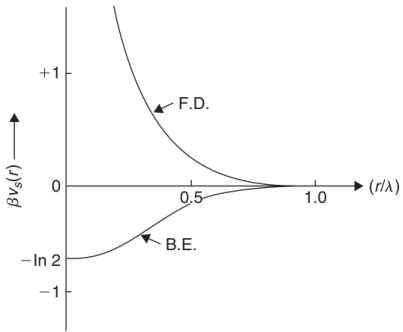
\includegraphics[width=0.36\textwidth]{images/chap5_m537b18d14f03bde19d574406a6848e1a.jpg}
\caption{一对遵循玻色-爱因斯坦统计或费米-狄拉克统计的粒子之间的统计势 \(v_{s}(r)\)。}
\label{fig:5_5.1}
\end{figure}

5.2. 证明：

\begin{equation}\tag{5.4.47}\label{eq:5.4.47}
\langle q | e ^{- \beta \hat { H} } | q ^{\prime} \rangle = \exp \left[ - \beta \hat { H } \left( - i \hbar \frac { \partial } { \partial q } , q \right) \right] \delta ( q - q ^{\prime} ) ,
\end{equation}

其中 \(\hat{H}(-i\hbar\,\partial/\partial q,q)\) 是系统在 \(q\) 表示下的哈密顿算符，该算符在形式上作用于狄拉克δ函数 \(\delta(q-q')\)。将δ函数展开为合适的形式，然后将这一结果应用于（i）自由粒子和（ii）线性谐振子。

推导出（i）自由粒子和（ii）线性谐振子在动量表示下的密度矩阵 \(\rho\)，并按照第 5.3 节的思路，研究其主要性质。

5.4. 以未对称化波函数（5.4.3）代替对称化波函数（5.5.7），研究自由粒子系统的密度矩阵及配分函数。表明，按照这一方法操作，既不会遇到吉布斯修正因子（1/N!），也不会出现粒子间的空间相关性。

5.5. 证明，在一阶近似下，由 \(N\) 个非相互作用、不可区分粒子组成的系统的配分函数可表示为：

\begin{equation}\tag{5.4.48}\label{eq:5.4.48}
Q _ { N } ( V , T ) = \frac { 1 } { N ! \lambda ^{3 N} } Z _ { N } ( V , T ) ,
\end{equation}

其中

\begin{equation}\tag{5.4.49}\label{eq:5.4.49}
Z _ { N } ( V , T ) = \int \exp \left\{ - \beta \sum _ { i < j } v _ { s } ( r _ { i j } ) \right\} d ^{3 N} r ,
\end{equation}

\(\nu_{s}(r)\) 为统计势（5.5.28）。进而计算该系统状态方程的一阶修正项。

5.6. 确定在标准状况下，氢、氦和氧的简并度判别式（\(n\lambda^{3}\)）的数值。估算这些量的相应温度范围，当其大小接近于 1 时，量子效应便开始变得显著。

5.7. 证明，一个由 \(N\) 个相互作用粒子组成的系统的量子力学配分函数，会趋近于经典形式。

\begin{equation}\tag{5.4.50}\label{eq:5.4.50}
Q _ { N } ( V , T ) = \frac { 1 } { N ! \, h ^{3 N} } \int e ^{- \beta E ( q , p )} d ^{3 N} q d ^{3 N} p
\end{equation}

随着平均热波长 \(\lambda\) 远远小于（i）粒子间平均距离 \((V/N)^{1/3}\)，以及（ii）粒子间势能的特征长度 \(r_0\) 时，系统的行为会趋于经典态。¹¹

5.8. 证明佩尔斯提出的以下定理。¹²

``若 \(\hat{H}\) 是给定物理系统的厄米哈密顿算符，而 \(\{\phi_{n}\}\) 是一组任意的正交波函数，且满足对称性要求以及边界条件\ldots\ldots{}''

问题的条件是，系统的配分函数满足以下不等式：

\begin{equation}\tag{5.4.51}\label{eq:5.4.51}
Q ( \beta ) \geq \sum _ { n } \exp \{ - \beta \langle \phi _ { n } | \hat { H } | \phi _ { n } \rangle \} ;
\end{equation}

当 \{\(\phi_{n}\)\} 构成哈密顿算符本身特征函数的完备正交集时，等号成立。


\chapter{简单气体理论}
如今，我们已完全掌握了用于推导多种物理系统宏观性质的正式理论框架。然而，在大多数情况下，推导过程往往面临严重的数学难题，因此人们不得不将分析范围限制在更简单的系统类型，或对实际系统进行简化建模。实际上，即便是在这些受限的研究中，分析过程也往往分阶段进行，而第一阶段的分析往往高度"理想化"。这种理想化的最佳范例，便是我们熟悉的理想气体——对其研究不仅有助于熟练掌握数学方法，还能深刻揭示自然界中真实存在的气体所表现出的物理行为。事实上，理想气体理论也正是建立在这一理想化基础之上的；详情请参见第~10~章。
在本章中，我们拟推导并详细探讨遵从量子统计规律的简单气体系统的最基本性质；讨论将涵盖双原子气体、多原子气体以及化学平衡等关键特征。
\section{在量子力学微正则系综中的理想气体}\label{ux5728ux91cfux5b50ux529bux5b66ux5faeux6b63ux5219ux7cfbux7efcux4e2dux7684ux7406ux60f3ux6c14ux4f53}
我们考虑一个由\(N\)个相互不干扰、彼此无法区分的粒子组成的气体系统，该系统被限制在体积为\(V\)的空间中，并共享给定的能量\(E\)。在这种情况下，我们所关注的统计量是\(\Omega(N,V,E)\)，其定义为：在宏观状态\((N,V,E)\)下，系统可达到的各不同微观状态的数量。在计算这一数量时，我们必须牢记：若未能以恰当的方式充分考虑粒子的不可区分性，所得到的结果在经典极限下可能并不成立，甚至可能难以接受。基于此，我们按照以下步骤进行推导。
由于在大体积的情况下，系统中单个粒子的能量级彼此非常接近，我们可以将能谱划分为大量"能级组"，这些组可被称为能量单元；详见图~6.1。设\(\varepsilon_i\)为某一能级的平均能量，\(g_i\)为第\(i\)个能量单元中的（任意）能级数量；我们假设所有\(g_i \gg 1\)。在特定情形下，我们可能会发现，第1个能量单元中有\(n_1\)个粒子，第2个能量单元中有\(n_2\)个粒子，以此类推。显然，分布序列\(\{n_i\}\)必须满足以下条件：
\begin{equation}\tag{6.1.1}\label{eq:6.1.1}
\sum _ { i } n _ { i } = N
\end{equation}
其中，\(W\{n_i\}\) 表示与分布集合 \(\{n_i\}\) 相关的不同微观状态数量；而求和符号 \(\prime\) 则对所有符合条件 (1) 和 (2) 的分布集合求和。接下来，
\begin{equation}\tag{6.1.2}\label{eq:6.1.2}
W ^{\{ n _ { i} \} } = \prod _ { i } w ( i ) ,
\end{equation}
其中，\(w(i)\) 表示与光谱中第 \(i\) 个能量单元相关联的不同微观状态数量（即包含 \(n_i\) 个粒子，并分布在该单元的 \(g_i\) 个能级上的微观态数），而乘积对光谱中所有能量单元求取。显然，\(w(i)\) 是将 \(n_i\) 个相同且不可区分粒子分配到第 \(i\) 个单元中 \(g_i\) 个能级的总方式数。在玻色-爱因斯坦情形下，这一数值由式（3.8.25）给出：
\begin{equation}\tag{6.1.3}\label{eq:6.1.3}
w _ { \mathrm { B . E . } } ( \vec { i } ) = \frac { ( n _ { i } + g _ { i } - 1 ) ! } { n _ { i } ! \, ( g _ { i } - 1 ) ! } ,
\end{equation}
因此，
\begin{equation}\tag{6.1.4}\label{eq:6.1.4}
W _ { \mathrm { B . E . } } \{ n _ { i } \} = \prod _ { i } \frac { ( n _ { i } + g _ { i } - 1 ) ! } { n _ { i } ! ( g _ { i } - 1 ) ! } .
\end{equation}
在费米-狄拉克情形下，任何一个能级都不能容纳超过一个粒子；因此，\(n_{i}\) 的值不能超过 \(g_{i}\)。此时，\(w(i)\) 的数值则由"将 \(g_{i}\) 个能级划分为两个子组——一个由 \(n_{i}\) 个能级组成（每个能级将各有一个粒子），另一个由 \((g_{i} - n_{i})\) 个能级组成（这些能级将空置）"的方式给出。这一数值由以下公式给出：
\begin{equation}\tag{6.1.5}\label{eq:6.1.5}
w _ { \mathrm { F . D . } } ( i ) = \frac { g _ { i } ! } { n _ { i } ! \left( g _ { i } - n _ { i } \right) ! } ,
\end{equation}
因此，
\begin{equation}\tag{6.1.6}\label{eq:6.1.6}
W _ { \mathrm { F . D . } } \{ n _ { i } \} = \prod _ { i } \frac { g _ { i } ! } { n _ { i } ! ( g _ { i } - n _ { i } ) ! } .
\end{equation}
为完整性起见，我们也可以纳入经典情形——或者说通常所称的麦克斯韦-玻尔兹曼情形。在该情形下，粒子被视为可区分的，因此任意一个 \(n_i\) 粒子均可独立地被置于任意一个 \(g_i\) 个能级中，且由此产生的各种态均可被视为彼此不同；这些态的数量显然为 \((g_i)^{n_i}\)。此外，在这种情形下，分布集合 \(\{n_i\}\) 本身也被视为可以被获得的，
\begin{equation}\tag{6.1.7}\label{eq:6.1.7}
\frac { N ! } { n _ { 1 } ! n _ { 2 } ! \ldots }
\end{equation}
通过不同的方式，当引入吉布斯修正因子后，会得到一个"权重因子"。
\begin{equation}\tag{6.1.8}\label{eq:6.1.8}
\frac { 1 } { n _ { 1 } ! n _ { 2 } ! \ldots } = \prod _ { i } \frac { 1 } { n _ { i } ! } ;
\end{equation}
另请参阅第 1.6 节，尤其是式 (1.6.2)。将这两个结果结合在一起，我们得到
\begin{equation}\tag{6.1.9}\label{eq:6.1.9}
W _ { \mathrm { M . B . } } \{ n _ { i } \} = \prod _ { i } \frac { ( g _ { i } ) ^{n _ { i} } } { n _ { i } ! } .
\end{equation}
现在，系统的熵将由以下公式给出：
\begin{equation}\tag{6.1.10}\label{eq:6.1.10}
S ( N , V , E ) = k \ln \Omega ( N , V , E ) = k \ln \left[ \sum _ { \{ n _ { i } \} } ^{\prime} W \{ n _ { i } \} \right] .
\end{equation}
可以证明，在我们分析所处的条件下，(12) 式右侧求和项的对数，可以近似为该求和中最大项的对数；请参阅问题 3.4。因此，我们可以将 (12) 式替换为
\begin{equation}\tag{6.1.11}\label{eq:6.1.11}
S ( N , V , E ) \approx k \ln W \{ n _ { i } ^{*} \} ,
\end{equation}
其中，\(n_{i}^{*}\) 是能够使 \(W\{n_{i}\}\) 数值达到最大化的分布集合；而 \(n_{i}^{*}\) 这些数值显然正是分布参数 \(n_{i}\) 的最可能取值。然而，这一最大化过程必须在约束条件下进行——即保持总量 \(N\) 和能量 \(E\) 保持恒定。这一问题可以通过拉格朗日乘数法来解决，具体参见第 3.2 节。现在，我们用来确定最可能分布集合 \(n_{i}^{*}\) 的条件，如\autoref{eq:6.1.1}、\autoref{eq:6.1.2} 和\autoref{eq:6.1.13} 所示，
\begin{equation}\tag{6.1.12}\label{eq:6.1.12}
\delta \ln W \{ n _ { i } \} - \left[ \alpha \sum _ { i } \delta n _ { i } + \beta \sum _ { i } \varepsilon _ { i } \delta n _ { i } \right] = 0 .
\end{equation}
对于 \(\ln W\{n_i\}\)，根据\autoref{eq:6.1.6}、\autoref{eq:6.1.8} 和\autoref{eq:6.1.11}，假设不仅所有 \(g_i\) 都足够大，而且所有 \(n_i\) 也均远大于 1（因此可以对这些表达式中出现的所有阶乘应用斯特林近似公式 \(\ln(x!) \approx x \ln x - x\)），
\begin{equation}\tag{6.1.13}\label{eq:6.1.13}
\begin{array}{rl} & { \ln W \{ n _ { i } \} = \sum _ { i } \ln w ( i ) } \\& {  \approx \sum _ { i } \left[ n _ { i } \ln \left( \frac { g _ { i } } { n _ { i } } - a \right) - \frac { g _ { i } } { a } \ln \left( 1 - a \frac { n _ { i } } { g _ { i } } \right) \right] , } \end{array}
\end{equation}
其中，对于 B.E. 情况，\(a = -1\)；对于 F.D. 情况，\(a = +1\)；而对于 M.B. 情况，\(a = 0\)。于是，\autoref{eq:6.1.14} 变为
\begin{equation}\tag{6.1.14}\label{eq:6.1.14}
\sum _ { i } \left[ \ln \left( \frac { g _ { i } } { n _ { i } } - \alpha \right) - \alpha - \beta \varepsilon _ { i } \right] _ { n _ { i } = n _ { i } ^{*} } \delta n _ { i } = 0 .
\end{equation}
鉴于\autoref{eq:6.1.16} 中增量 \(\delta n_{i}\) 的任意性，我们必然有（对于所有 \(i\)）
\begin{equation}\tag{6.1.15}\label{eq:6.1.15}
\ln \left( \frac { g _ { i } } { n _ { i } ^{*} } - a \right) - \alpha - \beta \varepsilon _ { i } = 0 ,
\end{equation}
因此，\(^{1}\)
\begin{equation}\tag{6.1.16}\label{eq:6.1.16}
n _ { i } ^{*} = \frac { g _ { i } } { e ^{\alpha + \beta \varepsilon _ { i} } + a } .
\end{equation}
\(n_{i}^{*}\) 与 \(g_{i}\) 成正比这一事实，促使我们对这一量进行如下解释：
\begin{equation}\tag{6.1.17}\label{eq:6.1.17}
\frac { n _ { i } ^{*} } { g _ { i } } = \frac { 1 } { e ^{\alpha + \beta \varepsilon _ { i} } + a } ,
\end{equation}
实际上，这一量正是第 \(i\) 个能级中每单位能量的粒子数——也就是单个能量水平 \(\varepsilon_i\) 中的最可能粒子数。顺便一提，我们的最终结果（18a）完全独立于粒子的能量水平的分组方式。
只要每个能级的层数足够多，粒子就会被分组到各个能级中。正如第 6.2 节所展示的那样，公式（18a）也可以完全不通过将能量水平分组为能级的方式来推导；事实上，只有在这种情况下，这一结果才真正具有可接受性！
将\autoref{eq:6.1.18} 代入\autoref{eq:6.1.15}，我们得到气体的熵为
\begin{equation}\tag{6.1.18}\label{eq:6.1.18}
\begin{array}{r} { \frac { S } { k } \approx \ln W \{ n _ { i } ^{*} \} = \sum _ { i } \left[ n _ { i } ^{*} \ln \left( \frac { g _ { i } } { n _ { i } ^{*} } - a \right) - \frac { g _ { i } } { a } \ln \left( 1 - a \frac { n _ { i } ^{*} } { g _ { i } } \right) \right] } \\{ = \sum _ { i } \left[ n _ { i } ^{*} \left( \alpha + \beta \varepsilon _ { i } \right) + \frac { g _ { i } } { a } \ln \left\{ 1 + a e ^{- \alpha - \beta \varepsilon _ { i} } \right\} \right] . } \end{array}
\end{equation}
\autoref{eq:6.1.19} 右侧的第一项同等于 \(\alpha N\)，而第二项则同等于 \(\beta E\)。因此，对于第三项，我们有
\begin{equation}\tag{6.1.19}\label{eq:6.1.19}
\frac { 1 } { a } \sum _ { i } g _ { i } \ln \left\{ 1 + a e ^{- \alpha - \beta \varepsilon _ { i} } \right\} = \frac { S } { k } - \alpha N - \beta E .
\end{equation}
如今，这里参数 \(\alpha\) 和 \(\beta\) 的物理意义，与第 4.3 节中的解释完全一致，即
\begin{equation}\tag{6.1.20}\label{eq:6.1.20}
\alpha = - \frac { \mu } { k T } ,  \beta = \frac { 1 } { k T } ;
\end{equation}
欲确认这一点，请参阅第 6.2 节。因此，\autoref{eq:6.1.20} 的右侧等于
\begin{equation}\tag{6.1.21}\label{eq:6.1.21}
\frac { S } { \bar { k } } + \frac { \mu N } { \bar { k } T } - \frac { E } { \bar { k } T } = \frac { G - ( E - T S ) } { k T } = \frac { P V } { \bar { k } T } .
\end{equation}
因此，系统的热力学压力由以下公式给出
\begin{equation}\tag{6.1.22}\label{eq:6.1.22}
P V = \frac { k T } { a } \sum _ { i } \left[ g _ { i } \ln \left\{ 1 + a e ^{- \alpha - \beta \varepsilon _ { i} } \right\} \right] .
\end{equation}
在麦克斯韦-玻尔兹曼情形下（\(a \rightarrow 0\)），\autoref{eq:6.1.23} 变为
\begin{equation}\tag{6.1.23}\label{eq:6.1.23}
P V = k T \sum _ { i } g _ { i } e ^{- \alpha - \beta \varepsilon _ { i} } = k T \sum _ { i } n _ { i } ^{*} = N k T ,
\end{equation}
这是经典理想气体所熟悉的状态方程。请注意，对于麦克斯韦-玻尔兹曼情形，式（24）成立，且与能量谱 \(\varepsilon_{i}\) 的具体细节无关。
人们会发现，式（23）中的表达式 \(a^{-1}\sum_i[\cdots]\) 与热力学量 \(PV/kT\) 相等，理应与理想气体的 \(q\)-势一致。因此，我们有望通过这一表达式获得该系统的所有宏观性质。不过，在进一步证明这一点之前，我们首先需要在正则系综与巨正则系综下，对理想气体理论进行系统性推导。
\section{其他量子力学系综下的理想气体}\label{ux5176ux4ed6ux91cfux5b50ux529bux5b66ux7edfux8ba1ux6001ux4e0bux7684ux7406ux60f3ux6c14ux4f53}
在正则系综中，某一系统的热力学性质是通过其配分函数推导得出的。
\begin{equation}\tag{6.2.1}\label{eq:6.2.1}
Q _ { N } ( V , T ) = \sum _ { E } e ^{- \beta E} ,
\end{equation}
其中 \(E\) 表示系统的能级，而 \(\beta = 1/kT\)。现在，我们可以将某一能量值 \(E\) 用单粒子能量 \(\varepsilon\) 来表示；例如，
\begin{equation}\tag{6.2.2}\label{eq:6.2.2}
E = \sum _ { \varepsilon } n _ { \varepsilon } \varepsilon ,
\end{equation}
其中 \(n_{\varepsilon}\) 是处于单粒子能量状态 \(\varepsilon\) 中的粒子数。这些数值 \(n_{\varepsilon}\) 必须满足以下条件：
\begin{equation}\tag{6.2.3}\label{eq:6.2.3}
\sum _ { \varepsilon } n _ { \varepsilon } = N .
\end{equation}
于是，式（1）可以写成：
\begin{equation}\tag{6.2.4}\label{eq:6.2.4}
Q _ { N } ( V , T ) = \sum _ { \{ n _ { \varepsilon } \} } ^{\prime} g \{ n _ { \varepsilon } \} e ^{- \beta \sum _ { \varepsilon} n _ { \varepsilon } \varepsilon } ,
\end{equation}
其中 \(g\{n_{\varepsilon}\}\) 是适用于分布集合 \(\{n_{\varepsilon}\}\) 的统计权重因子，而求和符号 \(\sum'\) 则遍历所有符合约束条件（3）的分布集合。不同情况下的统计权重因子分别为：
\begin{equation}\tag{6.2.5}\label{eq:6.2.5}
g _ { \mathrm { B . E . } } \{ n _ { \varepsilon } \} = 1 ,
\end{equation}
\begin{equation}\tag{6.2.6}\label{eq:6.2.6}
g _ { \mathrm { F . D . } } \{ n _ { \varepsilon } \} = \left\{ \begin{array}{ll} { 1 } & { \mathrm { i f ~ a l l ~ } n _ { \varepsilon } = 0 \mathrm { ~ o r ~ } 1 } \\{ 0 } & { \mathrm { o t h e r w i s e } , } \end{array} \right.
\end{equation}
并且
\begin{equation}\tag{6.2.7}\label{eq:6.2.7}
g _ { \mathrm { M . B . } } \{ n _ { \varepsilon } \} = \prod _ { \varepsilon } \frac { 1 } { n _ { \varepsilon } ! } .
\end{equation}
需要注意的是，在本研究中，我们处理的是单粒子态作为独立的状态，无需将其归入若干个"单元"之中；事实上，权重因子（5）、（6）和（7）均能直接从各自的前驱因子（6.1.6）、（6.1.8）和（6.1.11）中推导而来——只需将所有 \(g_i = 1\) 即可。
首先，我们先推导麦克斯韦-玻尔兹曼情形。将式（7）代入式（4），我们得到：
\begin{equation}\tag{6.2.8}\label{eq:6.2.8}
\begin{array}{r} { Q _ { N } ( V , T ) = \sum _ { \{ n _ { \varepsilon } \} } ^{\prime} \left[ \left( \prod _ { \varepsilon } \frac { 1 } { n _ { \varepsilon } ! } \right) \prod _ { \varepsilon } \left( e ^{- \beta \varepsilon} \right) ^{n _ { \varepsilon} } \right] } \\{ = \frac { 1 } { N ! } \sum _ { \{ n _ { \varepsilon } \} } ^{\prime} \left[ \frac { N ! } { \prod _ { \varepsilon } n _ { \varepsilon } ! } \prod _ { \varepsilon } \left( e ^{- \beta \varepsilon} \right) ^{n _ { \varepsilon} } \right] . } \end{array}
\end{equation}
由于这里的求和运算受制于条件（3），因此可以借助多项式定理进行计算，其结果为：
\begin{equation}\tag{6.2.9}\label{eq:6.2.9}
\begin{array}{r} { Q _ { N } ( V , T ) = \frac { 1 } { N ! } \left[ \sum _ { \varepsilon } e ^{- \beta \varepsilon} \right] ^{N} } \\{ = \frac { 1 } { N ! } [ Q _ { 1 } ( V , T ) ] ^{N} , } \end{array}
\end{equation}
这与式（3.5.15）的结果一致。当然，\(Q_{1}\) 的计算过程非常简单。利用单粒子能级介于 \(\varepsilon\) 与 \(\varepsilon + d\varepsilon\) 之间的数量的渐近公式（2.4.7），我们得以得出：
\begin{equation}\tag{6.2.10}\label{eq:6.2.10}
\begin{array}{rlr} & { } & { Q _ { 1 } ( V , T ) \equiv \sum _ { \varepsilon } e ^{- \beta \varepsilon} \approx \frac { 2 \pi V } { \hbar ^{3} } ( 2 m ) ^{3 / 2} \int _ { 0 } ^{\infty} e ^{- \beta \varepsilon} \varepsilon ^{1 / 2} d \varepsilon } \\& { } & { = V / \lambda ^{3} , } \end{array}
\end{equation}
其中，\(\lambda\) {[}等于 \(h/(2\pi mkT)^{1/2}\){]} 是粒子的平均热波长。因此，
\begin{equation}\tag{6.2.11}\label{eq:6.2.11}
Q _ { N } ( V , T ) = \frac { V ^{N} } { N ! \lambda ^{3 N} } ,
\end{equation}
由此可推导出该系统的完整热力学关系；例如，请参阅第 3.5 节。此外，我们还得到了该系统的巨配分函数
\begin{equation}\tag{6.2.12}\label{eq:6.2.12}
\mathcal { Q } ( z , V , T ) = \sum _ { N = 0 } ^{\infty} z ^{N} Q _ { N } ( V , T ) = \exp ( z V / \lambda ^{3} ) ;
\end{equation}
与\autoref{eq:4.4.3} 进行比较。我们知道，该系统的热力学同样可以由 \(\mathcal{Q}\) 的表达式完美地推导出来。
在玻色-爱因斯坦和费米-狄拉克两种情形下，我们将 (5) 和 (6) 代入 (4)，即可得到：
\begin{equation}\tag{6.2.13}\label{eq:6.2.13}
Q _ { N } ( V , T ) = \sum _ { \{ n _ { \varepsilon } \} } ^{\prime} \left( e ^{- \beta \sum _ { \varepsilon} n _ { \varepsilon } \varepsilon } \right) ;
\end{equation}
B.E. 和 F.D. 两种情形之间的差异，源于数值 \(n_{\varepsilon}\) 可取的不同取值。鉴于求和符号 \(\sum'\) 所受的限制，要在这些情形中对配分函数 \(Q_{N}\) 进行明确计算，显得相当繁琐。相比之下，巨配分函数 \(\mathcal{Q}\) 却更容易处理；我们有
\begin{equation}\tag{6.2.14}\label{eq:6.2.14}
\begin{array}{r} { \mathcal { Q } ( z , V , T ) = \displaystyle \sum _ { N = 0 } ^{\infty} \left[ z ^{N} \sum _ { \{ n _ { \varepsilon } \} } ^{\prime} e ^{- \beta \sum _ { \varepsilon} n _ { \varepsilon } \varepsilon } \right] } \\{ = \displaystyle \sum _ { N = 0 } ^{\infty} \left[ \sum _ { \{ n _ { \varepsilon } \} } ^{\prime} \prod _ { \varepsilon } \left( z e ^{- \beta \varepsilon} \right) ^{n _ { \varepsilon} } \right] . } \end{array}
\end{equation}
现在，\autoref{eq:6.2.14} 中的双重求和——先对满足总数量 \(N\) 固定值约束的数值 \(n_{\varepsilon}\) 进行求和，再对所有可能的 \(N\) 值进行求和——实际上等同于对所有可能的 \(n_{\varepsilon}\) 值进行求和，且彼此之间互不相关。因此，我们可以写作
\begin{equation}\tag{6.2.15}\label{eq:6.2.15}
\begin{array}{rl} & { \mathcal { Q } ( z , V , T ) = \sum _ { n _ { 0 } , n _ { 1 } , \ldots } \left[ \left( z e ^{- \beta \varepsilon _ { 0} } \right) ^{n _ { 0} } \left( z e ^{- \beta \varepsilon _ { 1} } \right) ^{n _ { 1} } \ldots \right] } \\& {  = \left[ \sum _ { n _ { 0 } } \left( z e ^{- \beta \varepsilon _ { 0} } \right) ^{n _ { 0} } \right] \left[ \sum _ { n _ { 1 } } \left( z e ^{- \beta \varepsilon _ { 1} } \right) ^{n _ { 1} } \right] \ldots . } \end{array}
\end{equation}
在玻色-爱因斯坦情形下，\(n_{s}\) 可以是 0、1、2\ldots\ldots；而在费米-狄拉克情形下，\(n_{s}\) 只能是 0 或 1。因此，
\begin{equation}\tag{6.2.16}\label{eq:6.2.16}
\mathcal { Q } ( z , V , T ) = \left\{ \begin{array}{ll} { \displaystyle \prod _ { \varepsilon } \frac { 1 } { ( 1 - z e ^{- \beta \varepsilon} ) } } & { \mathrm { i n ~ t h e ~ B . E . ~ c a s e , ~ w i t h ~ z e ^{- \beta \varepsilon} < 1 } } \\{ \displaystyle \prod _ { \varepsilon } ( 1 + z e ^{- \beta \varepsilon} ) } & { \mathrm { i n ~ t h e ~ F . D . ~ c a s e . } } \end{array} \right.
\end{equation}
系统的 \(q\) 势由此给出为
\begin{equation}\tag{6.2.17}\label{eq:6.2.17}
\begin{array}{r} { q ( z , V , T ) \equiv \frac { P V } { k T } \equiv \ln \mathcal { Q } ( z , V , T ) } \\{ = \mp \sum _ { \varepsilon } \ln ( 1 \mp z e ^{- \beta \varepsilon} ) ; } \end{array}
\end{equation}
与\autoref{eq:6.1.23} 进行比较，其中 \(g_{i}=1\)。将逸度（fugacity）\(z\) 与\autoref{eq:6.1.23} 中的量 \(e^{-\alpha}\) 对应是自然的；相应地，\(\alpha=-\mu/kT\)。一如往常，\autoref{eq:6.2.17} 中的上（下）符号分别对应于玻色（费米）情形。
最终，我们可以将 \(q\) 的结果以适用于三种情形的形式写成：
\begin{equation}\tag{6.2.18}\label{eq:6.2.18}
q ( z , V , T ) \equiv \frac { P V } { k T } = \frac { 1 } { a } \sum _ { \varepsilon } \ln ( 1 + a z e ^{- \beta \varepsilon} ) ,
\end{equation}
其中 \(a = -1\)、\(+1\) 或 \(0\)，具体取决于支配该系统的统计规律。尤其是，经典情形（\(a \rightarrow 0\)）给出了
\begin{equation}\tag{6.2.19}\label{eq:6.2.19}
q _ { \mathrm { M . B . } } = z \sum _ { \varepsilon } e ^{- \beta \varepsilon} = z Q _ { 1 } ,
\end{equation}
与\autoref{eq:4.4.4} 相一致。从\autoref{eq:6.2.18} 可知，
\begin{equation}\tag{6.2.20}\label{eq:6.2.20}
\overline { { N } } \equiv z \left( \frac { \partial q } { \partial z } \right) _ { V , T } = \sum _ { \varepsilon } \frac { 1 } { z ^{- 1} e ^{\beta \varepsilon} + a }
\end{equation}
并且
\begin{equation}\tag{6.2.21}\label{eq:6.2.21}
\overline { { E } } \equiv - \left( \frac { \partial q } { \partial \beta } \right) _ { z , V } = \sum _ { \varepsilon } \frac { \varepsilon } { z ^{- 1} e ^{\beta \varepsilon} + a } .
\end{equation}
与此同时，能量水平 \(\varepsilon\) 的平均占据数 \(\langle n_{\varepsilon}\rangle\) 也得以确定，详见\autoref{eq:6.2.14} 和\autoref{eq:6.2.17}，
\begin{equation}\tag{6.2.22}\label{eq:6.2.22}
\begin{array}{rl} & { \langle n _ { \varepsilon } \rangle = \frac { 1 } { Q } \left[ - \frac { 1 } { \beta } \left( \frac { \partial \mathcal { Q } } { \partial \varepsilon } \right) _ { z , T , \mathrm { ~ a l l ~ o t h e r ~ } \varepsilon } \right] } \\& { \equiv - \frac { 1 } { \beta } \left( \frac { \partial q } { \partial \varepsilon } \right) _ { z , T , \mathrm { ~ a l l ~ o t h e r ~ } \varepsilon } } \\& { = \frac { 1 } { z ^{- 1} e ^{\beta \varepsilon} + a } , } \end{array}
\end{equation}
与式（20）和式（21）相一致。将我们的最终结果（22）与其对应项（6.1.18a）进行比较，我们发现，单粒子态的占据数 \(n\) 的平均值 \(\langle n \rangle\) 与最可能值 \(n^{*}\) 确实完全相同。
\section{占据数的统计性质}\label{ux503eux5411ux6570ux7684ux7edfux8ba1ux6027ux8d28}
式（6.2.22）将单粒子态的能量为 \(\varepsilon\) 时的平均占据数，以 \((\varepsilon - \mu)/kT\) 这一量的显式函数形式给出：
\begin{equation}\tag{6.3.1}\label{eq:6.3.1}
\langle n _ { \varepsilon } \rangle = \frac { 1 } { e ^{( \varepsilon - \mu ) / k T} + a } .
\end{equation}
该数量的函数行为如图~6.2所示。在费米-狄拉克情形下（\(a=+1\)），平均占据数永远不会超过 1，因为变量 \(n_{\varepsilon}\) 本身只能取 0 或 1。此外，当 \(\varepsilon<\mu\) 且 \(|\varepsilon-\mu|\gg kT\) 时，平均占据数会趋近于其最大可能值 1。而在玻色-爱因斯坦情形下（\(a=-1\)），必须满足 \(\mu < \varepsilon\)（对所有单粒子能级）；请参见式（6.2.16a）。事实上，当 \(\mu\) 等于最低能级 \(\varepsilon_0\) 时，该特定能级的占据数会无限增大，从而引发玻色-爱因斯坦凝聚现象；详见第7.1节和第7.2节。对于
这与条件（5.5.20）相一致。
接下来，我们将考察变量 \(n_{\varepsilon}\) 的统计涨落。在对导致式（6.2.22）的计算进行进一步推导后，我们得到
\begin{equation}\tag{6.3.2}\label{eq:6.3.2}
\langle n _ { \varepsilon } ^{2} \rangle = \frac { 1 } { Q } \left[ \left( - \frac { 1 } { \beta } \frac { \partial } { \partial \varepsilon } \right) ^{2} Q \right] _ { z , T , \mathrm { ~ a l l ~ o t h e r ~ } \varepsilon } ;
\end{equation}
由此可得
\begin{equation}\tag{6.3.3}\label{eq:6.3.3}
\begin{array}{rl} & { \langle n _ { \varepsilon } ^{2} \rangle - \langle n _ { \varepsilon } \rangle ^{2} = \left[ \left( - \frac { 1 } { \beta } \frac { \partial } { \partial \varepsilon } \right) ^{2} \ln \mathcal { Q } \right] _ { z , T , \mathrm { ~ a l l ~ o t h e r ~ } \varepsilon } } \\& {  = \left[ \left( - \frac { 1 } { \beta } \frac { \partial } { \partial \varepsilon } \right) \langle n _ { \varepsilon } \rangle \right] _ { z , T } . } \end{array}
\end{equation}
对于相对均方差，我们得出结果（无论粒子遵循何种统计分布）
\begin{equation}\tag{6.3.4}\label{eq:6.3.4}
\frac { \langle n _ { \varepsilon } ^{2} \rangle - \langle n _ { \varepsilon } \rangle ^{2} } { \langle n _ { \varepsilon } \rangle ^{2} } = \left( \frac { 1 } { \beta } \frac { \partial } { \partial \varepsilon } \right) \left\{ \frac { 1 } { \langle n _ { \varepsilon } \rangle } \right\} = z ^{- 1} e ^{\beta \varepsilon} ;
\end{equation}
当然，这一量的实际数值将取决于粒子的统计分布，因为在给定的粒子密度（\(N/V\)）和给定的温度 \(T\) 下，不同统计分布下 \(z\) 的取值也会有所不同。
将式（8）改写成如下形式，似乎更具启发性
\begin{equation}\tag{6.3.5}\label{eq:6.3.5}
\frac { \langle n _ { \varepsilon } ^{2} \rangle - \langle n _ { \varepsilon } \rangle ^{2} } { \langle n _ { \varepsilon } \rangle ^{2} } = \frac { 1 } { \langle n _ { \varepsilon } \rangle } - a .
\end{equation}
在经典情形下（\(a=0\)），相对涨落呈正态分布。而在费米-狄拉克情形下，相对涨落的表达式为 \(1/\langle n_{\varepsilon}\rangle-1\)，其值低于正常水平，并随着 \(\langle n_{\varepsilon}\rangle\) 趋近于1而逐渐趋于零。而在玻色-爱因斯坦情形下，涨落明显高于正常水平。² 显然，这一结论同样适用于光子气体，进而也适用于黑体辐射中的振子态。在后一种情境下，爱因斯坦早在1909年便依据普朗克的方法推导出了这一结果，并指出，涨落表达式中的项1可能源于辐射的波动特性，而项 \(1/\langle n_{\varepsilon}\rangle\) 则源自光子的粒子特性；有关详细内容，请参阅基特尔（1958）和特尔哈尔回顾（1968）。
与涨落问题密切相关的是"光子束中的统计相关性"这一问题，这一现象已通过实验被观测到（参见汉伯里·布朗和
Twiss（1956年、1957年、1958年）曾对这些涨落的量子统计性质进行了理论阐释（参见Purcell，1956年；Kothari与Auluck，1957年）。如需更多详细信息，请参考Mandel、Sudarshan和Wolf（1964年）以及Holliday与Sage（1964年）的相关文献。
为了更深入地理解占有数的统计特性，我们来计算量 \(p_{\varepsilon}(n)\)——即在能量为 \(\varepsilon\) 的状态中恰好存在 \(n\) 个粒子的概率。根据式（6.2.14b），我们可以推导出 \(p_{\varepsilon}(n) \propto (ze^{-\beta\varepsilon})^{n}\)。经过归一化处理后，在玻色-爱因斯坦情形下，该表达式变为：
\begin{equation}\tag{6.3.6}\label{eq:6.3.6}
\begin{array}{r} { p _ { \varepsilon } ( n ) | _ { \mathrm { B . E . } } = \left( z e ^{- \beta \varepsilon} \right) ^{n} \left[ 1 - z e ^{- \beta \varepsilon} \right] } \\{ = \left( \frac { \langle n _ { \varepsilon } \rangle } { \langle n _ { \varepsilon } \rangle + 1 } \right) ^{n} \frac { 1 } { \langle n _ { \varepsilon } \rangle + 1 } = \frac { ( \langle n _ { \varepsilon } \rangle ) ^{n} } { ( \langle n _ { \varepsilon } \rangle + 1 ) ^{n + 1} } . } \end{array}
\end{equation}
在费米-狄拉克情形下，我们得到
\begin{equation}\tag{6.3.7}\label{eq:6.3.7}
\begin{array}{r} { p _ { \varepsilon } ( n ) | _ { \mathrm { F . D . } } = \left( z e ^{- \beta \varepsilon} \right) ^{n} \left[ 1 + z e ^{- \beta \varepsilon} \right] ^{- 1} } \\{ = \left\{ \begin{array}{ll} { 1 - \langle n _ { \varepsilon } \rangle } & { \mathrm { f o r }  n = 0 } \\{ \langle n _ { \varepsilon } \rangle } & { \mathrm { f o r }  n = 1 . } \end{array} \right. } \end{array}
\end{equation}
在麦克斯韦-玻尔兹曼情形下，我们得到 \(p_{\varepsilon}(n) \propto (ze^{-\beta\varepsilon})^{n}/n!\)，而非原来的 \(p_{\varepsilon}(n)\)；请参阅式（6.2.8）。经过归一化处理后，我们得到
\begin{equation}\tag{6.3.8}\label{eq:6.3.8}
p _ { \varepsilon } ( n ) | _ { \mathrm { M . B . } } = \frac { \left( z e ^{- \beta \varepsilon} \right) ^{n} / n ! } { \exp \left( z e ^{- \beta \varepsilon} \right) } = \frac { ( \langle n _ { \varepsilon } \rangle ) ^{n} } { n ! } e ^{- \langle n _ { \varepsilon} \rangle } .
\end{equation}
式（6.3.8）对应的是泊松分布，其变量方差等于其平均值本身；可与式（6.3.5）在 \(a=0\) 时进行对比。它也与理想经典系统构成的巨正则系综中总粒子数 \(N\) 的分布相似；请参阅问题4.4。此外，我们还注意到，在这种情况下，\(p_{\varepsilon}(n)/p_{\varepsilon}(n-1)\) 的比值会随着 \(n\) 的增大而呈反比关系，这正是无相关事件所遵循的“正常”统计行为。
另一方面，玻色-爱因斯坦情形下的分布则是几何分布，其公比为 \(\langle n_{\varepsilon}\rangle/(\langle n_{\varepsilon}\rangle+1)\)。这意味着，一个状态 \(\varepsilon\) 自身再增加一个粒子的概率，与该状态已占据的粒子数量无关；因此，与"正常"的统计行为相比，玻色子表现出一种特殊的"成簇"倾向，即它们之间存在正向的统计关联性。相比之下，费米子则呈现出负向的统计关联性。
\section{动力学考量}\label{ux52a8ux529bux5b66ux8003ux91cf}
理想气体的热力学压力由式（6.1.23）或（6.2.18）给出。鉴于体积 \(V\) 很大，单个粒子的能量态 \(\varepsilon\) 之间的距离将非常接近。
彼此十分接近，以至于对它们的求和可以替换为积分。由此，我们得到
\begin{equation}\tag{6.4.1}\label{eq:6.4.1}
\begin{array}{rl} & { P = \frac { k T } { a } \int _ { 0 } ^{\infty} \ln \Big [ 1 + a z e ^{- \beta \varepsilon ( p )} \Big ] \frac { 4 \pi \, p ^{2} d p } { h ^{3} } } \\& {  = \frac { 4 \pi \, k T } { a h ^{3} } \left[ \frac { p ^{3} } { 3 } \ln \Big [ 1 + a z e ^{- \beta \varepsilon ( p )} \Big ] \Big | _ { 0 } ^{\infty} + \int _ { 0 } ^{\infty} \frac { p ^{3} } { 3 } \frac { a z e ^{- \beta \varepsilon ( p )} } { 1 + a z e ^{- \beta \varepsilon ( p )} } \beta \frac { d \varepsilon } { d p } d p \right] . } \end{array}
\end{equation}
积分部分在两个极限处都趋近于零，而表达式的其余部分则简化为
\begin{equation}\tag{6.4.2}\label{eq:6.4.2}
P = \frac { 4 \pi } { 3 h ^{3} } \int _ { 0 } ^{\infty} \frac { 1 } { z ^{- 1} e ^{\beta \varepsilon ( p )} + a } \left( p \frac { d \varepsilon } { d p } \right) p ^{2} d p .
\end{equation}
现在，系统的总粒子数由
\begin{equation}\tag{6.4.3}\label{eq:6.4.3}
N = \int \langle n _ { p } \rangle \frac { V d ^{3} p } { h ^{3} } = \frac { 4 \pi V } { h ^{3} } \int _ { 0 } ^{\infty} \frac { 1 } { z ^{- 1} e ^{\beta \varepsilon ( p )} + a } p ^{2} d p .
\end{equation}
将式（1）与式（2）进行比较，我们可以写出
\begin{equation}\tag{6.4.4}\label{eq:6.4.4}
P = \frac { 1 } { 3 } \frac { N } { V } \left\langle p \frac { d \varepsilon } { d p } \right\rangle = \frac { 1 } { 3 } n \langle p u \rangle ,
\end{equation}
其中，\(n\) 为气体中的粒子密度，\(u\) 为单个粒子的速度。若能量 \(\varepsilon\) 与动量 \(p\) 的关系形式为 \(\varepsilon \propto p^{s}\)，则
\begin{equation}\tag{6.4.5}\label{eq:6.4.5}
P = \frac { s } { 3 } n \langle \varepsilon \rangle = \frac { s } { 3 } \frac { E } { V } ;
\end{equation}
特别地，当 \(s=1\) 和 \(s=2\) 时，其具体情形很容易识别。需要指出的是，式（3）和式（4）的结论与粒子所遵循的统计分布无关。
式（3）的结构表明，气体的压力本质上源自粒子的物理运动；因此，它应当仅凭动力学原理便可推导出来。为此，我们考虑气体中的粒子对容器壁的轰击作用。以图~6.3中的一侧壁为例，取一个面积为 \(dA\) 的元素，该元素与 z 轴方向正交。将注意力集中在那些速度介于 \(\boldsymbol{u}\) 与 \(\boldsymbol{u}+\boldsymbol{du}\) 之间的粒子上；单位体积内此类粒子的数量可记作 \(nf(\boldsymbol{u})du\)，其中
\begin{equation}\tag{6.4.6}\label{eq:6.4.6}
\intop_{\mathrm{all~}\boldsymbol{u}}f(\boldsymbol{u})d\boldsymbol{u}=1.
\end{equation}
\begin{equation}\tag{6.4.7}\label{eq:6.4.7}
P = 2 n  \int _ { u _ { x } = - \infty } ^{\infty} \int _ { u _ { y } = - \infty } ^{\infty} \int _ { u _ { z } = 0 } ^{\infty} p _ { z } u _ { z } f ( u ) d u _ { x } d u _ { y } d u _ { z } .
\end{equation}
由于（i）\(f(\boldsymbol{u})\) 仅依赖于 \(u\)，而（ii）乘积 \((p_{z}u_{z})\) 是 \(u_{z}\) 的偶函数，上述结果可写成
\begin{equation}\tag{6.4.8}\label{eq:6.4.8}
P = n \int \left( p _ { z } u _ { z } \right) f ( u ) d u .
\end{equation}
将式（7）与式（5）进行比较，我们得到
\begin{equation}\tag{6.4.9}\label{eq:6.4.9}
\begin{array}{rl} & { P = n \langle p _ { z } u _ { z } \rangle = n \langle p u \cos ^{2} \theta \rangle } \\& { = \frac { 1 } { 3 } n \langle p u \rangle , } \end{array}
\end{equation}
这一结果与式（3）完全相同。
³显然，只有那些 \(u_{z} > 0\) 的速度才在此处具有实际意义。
以类似的方式，我们还可以确定气体粒子通过壁上某一孔洞（面积为单位）的扩散速率。这一速率由下式给出，与式（6）相比，
\begin{equation}\tag{6.4.10}\label{eq:6.4.10}
\begin{array}{rl} { R = n } & { \int _ { u _ { x } = - \infty } ^{\infty} \int _ { u _ { y } = - \infty } ^{\infty} \int _ { u _ { z } = 0 } ^{\infty} u _ { z } f ( u ) d u _ { x } d u _ { y } d u _ { z } } \\& { = n \int _ { \phi = 0 } ^{2 \pi} \int _ { \theta = 0 } ^{\pi / 2} \int _ { u = 0 } ^{\infty} \{ u \cos \theta f ( u ) \} ( u ^{2} \sin \theta \, d u d \theta \, d \phi ) ; } \end{array}
\end{equation}
请注意，条件 \(u_{z} > 0\) 限制了角度 \(\theta\) 的取值范围，即从 0 到 \(\pi/2\)。通过对 \(\theta\) 和 \(\phi\) 进行积分，我们得到
\begin{equation}\tag{6.4.11}\label{eq:6.4.11}
R = n \pi \int _ { 0 } ^{\infty} f ( \mathbf { u } ) u ^{3} \, d \mathbf { u } .
\end{equation}
鉴于以下事实，
\begin{equation}\tag{6.4.12}\label{eq:6.4.12}
\int _ { 0 } ^{\infty} f ( u ) ( 4 \pi \, u ^{2} \, d u ) = 1 ,
\end{equation}
方程（12）可以写成
\begin{equation}\tag{6.4.13}\label{eq:6.4.13}
R = \frac { 1 } { 4 } n \langle u \rangle .
\end{equation}
再次强调，这一结果与粒子所遵循的统计规律无关。
显而易见，逸出粒子的速度分布与容器内粒子的速度分布有着显著差异。其原因在于：首先，逸出粒子的 \(u_{z}\) 速度分量必须为正（这在分布中引入了一定的各向异性）；其次，\(u_{z}\) 值较大的粒子会以更高的权重出现，而该权重与 \(u_{z}\) 的值成正比——详见方程（10）。因此，一方面，逸出粒子携带着净向前动量，从而导致容器产生反冲力；另一方面，每粒粒子携带的能量相对较高，使得容器中的气体不仅压力和密度不断下降，温度也逐渐降低——参见问题 6.14。
\section{由具有内部运动的分子构成的气体系统}\label{ux7531ux5177ux6709ux5185ux90e8ux8fd0ux52a8ux7684ux5206ux5b50ux6784ux6210ux7684ux6c14ux4f53ux7cfbux7edf}
在我们迄今为止的大多数研究中，我们仅考虑了分子运动的平移部分。尽管这种运动形式在气体系统中始终存在，但其他
方面，本质上与分子的内部运动有关，也同样存在。在计算此类系统的物理性质时，自然会将这些运动所产生的贡献纳入考量。在此过程中，我们假定：(i) 分子间相互作用的影响可以忽略不计，以及 (ii) 非简并性准则
\begin{equation}\tag{6.5.1}\label{eq:6.5.1}
n \lambda ^{3} = \frac { n h ^{3} } { ( 2 \pi m k T ) ^{3 / 2} } \ll 1
\end{equation}
已得到满足；这使我们的系统成为理想气体、玻尔兹曼气体。在这些假设下——而在大量应用中，这些假设往往能很好地成立——系统的配分函数可表示为
\begin{equation}\tag{6.5.2}\label{eq:6.5.2}
Q _ { N } ( V , T ) = \frac { 1 } { N ! } [ Q _ { 1 } ( V , T ) ] ^{N} ,
\end{equation}
其中
\begin{equation}\tag{6.5.3}\label{eq:6.5.3}
Q _ { 1 } ( V , T ) = \frac { V } { \lambda ^{3} } j ( T ) ;
\end{equation}
方括号内的因子正是我们熟悉的分子平移配分函数，而 \(j(T)\) 则是对应于内部运动的配分函数。后者可以写成
\begin{equation}\tag{6.5.4}\label{eq:6.5.4}
j ( T ) = \sum _ { i } g _ { i } e ^{- \varepsilon _ { i} / k T } ,
\end{equation}
其中 \(\varepsilon_{i}\) 是与内部运动状态相关联的能量（由量子数 \(i\) 表征），而 \(g_{i}\) 则是该状态的多重度。
分子内部运动所作出的贡献，除了平移自由度之外，可直接从函数 \(j(T)\) 中推导得出。我们得到
\begin{equation}\tag{6.5.5}\label{eq:6.5.5}
A _ { \mathrm { i n t } } = - N k T \ln j ,
\end{equation}
\begin{equation}\tag{6.5.6}\label{eq:6.5.6}
\mu _ { \mathrm { i n t } } = - k T \ln j ,
\end{equation}
\begin{equation}\tag{6.5.7}\label{eq:6.5.7}
S _ { \mathrm { i n t } } = N k \left( \ln j + T \frac { \partial } { \partial T } \ln j \right) ,
\end{equation}
\begin{equation}\tag{6.5.8}\label{eq:6.5.8}
U _ { \mathrm { i n t } } = N k T ^{2} \, \frac { \partial } { \partial T } \ln j ,
\end{equation}
并且
\begin{equation}\tag{6.5.9}\label{eq:6.5.9}
( C _ { V } ) _ { \mathrm { i n t } } = N k \frac { \partial } { \partial T } \left\{ T ^{2} \frac { \partial } { \partial T } \ln j \right\} .
\end{equation}
因此，本研究的核心问题在于：在已知分子内部状态的前提下，如何推导出函数 \(j(T)\) 的显式表达式。为此，我们注意到，分子的内部状态由以下四个要素决定：(i) 电子态，(ii) 核心态，(iii) 振动态，以及 (iv) 旋转态。严格来说，这四种激发模式之间相互作用；然而，在许多情况下，它们可以被独立地加以处理。于是，我们可以写出
\begin{equation}\tag{6.5.10}\label{eq:6.5.10}
j ( T ) = j _ { \mathrm { e l e c } } ( T ) j _ { \mathrm { n u c } } ( T ) j _ { \mathrm { v i b } } ( T ) j _ { \mathrm { r o t } } ( T ) ,
\end{equation}
由此可知，分子内部运动对系统各项热力学性质所作的净贡献，可表示为这四种贡献的简单求和。不过，在同核分子（如 AA）的情形下，有一种相互作用发挥着特殊的作用，即核态与旋转态之间的相互作用。在这种情况下，我们不妨改写为
\begin{equation}\tag{6.5.11}\label{eq:6.5.11}
j ( T ) = j _ { \mathrm { e l e c } } ( T ) j _ { \mathrm { n u c - r o t } } ( T ) j _ { \mathrm { v i b } } ( T ) .
\end{equation}
接下来，我们将按照复杂程度递增的顺序，对各类体系展开这一问题的研究。
\section{单原子分子}\label{ux5355ux539fux5b50ux5206ux5b50}
为简化起见，我们考虑一种单原子气体，其温度使得热能 \(kT\) 与电离能 \(\varepsilon_{\mathrm{ion}}\) 相比微不足道；对于不同的原子而言，这一条件大致为 \(T \ll \varepsilon_{\mathrm{ion}} / k \sim 10^{4}-10^{5} \mathrm{K}\)。在这样的温度下，气体中电离原子的数量几乎可以忽略不计。同样，处于激发态的原子亦然——因为任何激发态与原子基态之间的能级差，通常都与电离能本身处于同一数量级。因此，我们可以将气体中的所有原子都视为处于其（电子）基态。
如今，有一类特殊的原子，即氦、氖、氩等，它们在基态下既不具有轨道角动量，也不具有自旋（\(L = S = 0\)）。它们的（电子）基态显然为单重态，且 \(g_e = 1\)。然而，原子核却存在一种简并度，这种简并度源于原子核自旋可能存在的不同取向。⁴ 如果该自旋的值为 \(S_n\)，则相应的简并因子 \(g_n = 2S_n + 1\)。此外，单原子分子不可能具备任何振动态或旋转态。因此，此类分子的内部配分函数（3a）可表示为
\begin{equation}\tag{6.5.12}\label{eq:6.5.12}
j ( T ) = ( g ) _ { \mathrm { g r . s t . } } = g e \cdot g n = 2 S _ { n } + 1 .
\end{equation}
众所周知，核自旋的存在会在电子态中产生所谓的超精细结构。然而，该结构的能级间隔在几乎所有我们所关心的温度范围内，都远小于 \(kT\)；具体而言，这些能级间隔对应的温度范围大约为 \(10^{-1}\) 到 \(10^{0}\) K。因此，在计算分立函数 \(j(T)\) 时，可以忽略电子态的超精细分裂，而可通过一个简并因子来考虑核自旋所带来的多重度。
方程（4）至（8）告诉我们，在这种情况下，原子的内部运动仅会对气体的化学势和熵等性质作出贡献；它们并不会对内能和比热产生贡献。
另一方面，如果基态不具有轨道角动量，却具有自旋（\(L=0\), \(S\neq0\)——例如，碱金属原子的情况），那么基态仍然不会出现精细结构；不过，它将具有一个简并度 \(g_{e}=2S+1\)。因此，内部分立函数 \(j(T)\) 将被乘以一个 \((2S+1)\) 的因子，而气体的化学势和熵等性质也会相应地发生改变。
在其他情况下，原子的基态可能同时具有轨道角动量和自旋（\(L \neq 0, S \neq 0\)）；此时，基态将呈现出明确的精细结构。一般来说，该结构的能级间隔与 \(kT\) 相当；因此，在计算分立函数时，必须将精细结构各组成部分的能量纳入考量。由于这些组成部分的总角动量 \(J\) 各不相同，相应的分立函数可写为
\begin{equation}\tag{6.5.13}\label{eq:6.5.13}
j _ { \mathrm { e l e c } } ( T ) = \sum _ { J } ( 2 J + 1 ) e ^{- \varepsilon _ { J} / k T } .
\end{equation}
上述表达式在以下极限情况下会大大简化：
（a）当 \(kT \gg \varepsilon_J\) 时，
\begin{equation}\tag{6.5.14}\label{eq:6.5.14}
j _ { \mathrm { e l e c } } ( T ) \simeq \sum _ { J } ( 2 J + 1 ) = ( 2 L + 1 ) ( 2 S + 1 ) .
\end{equation}
（b）当 \(kT \ll \varepsilon_J\) 时，
\begin{equation}\tag{6.5.15}\label{eq:6.5.15}
j _ { \mathrm { e l e c } } ( T ) \simeq ( 2 J _ { 0 } + 1 ) e ^{- \varepsilon _ { 0} / k T } ,
\end{equation}
其中 \(J_{0}\) 是原子在最低能态下的总角动量，\(\varepsilon_{0}\) 是该原子在最低能态下的能量。无论哪种情况，电子运动均不对气体的比热作出贡献。当然，在中温条件下，我们确实会观察到这一属性的贡献。而且，鉴于无论在高温还是低温下，比热往往趋近于平移部分的值 \(\frac{3}{2}Nk\)，其在某一与精细结构能级间距相当的温度下，必然会经历一个最大值。⁵ 不用多说，每种情况下都必须考虑核自旋所带来的多重度 \((2S_{n}+1)\)。
\section{B 二原子分子}\label{b-ux4e8cux539fux5b50ux5206ux5b50}
现在我们来考虑一种二原子气体，其温度使得 \(kT\) 相对于解离能而言非常小；对于不同的分子而言，这再次等同于以下条件：
\(T \ll \varepsilon_{\mathrm{diss}} / k \sim 10^{4}-10^{5} \mathrm{K}\)。在这些温度下，气体中解离的分子数量几乎可以忽略不计。与此同时，在大多数情况下，激发态的分子也几乎不存在，因为将任何一种激发态与分子的基态相分离，其能量一般与解离能本身相当。因此，在对 \(j(T)\) 进行计算时，我们只需考虑分子的最低电子态。
在大多数情况下，最低电子态是无简并的：\(g_{e}=1\)。此时，我们无需再进一步考虑电子态如何为气体的热力学性质作出贡献。然而，某些分子（尽管数量并不多）在其最低电子态中，要么（i）具有非零轨道角动量（\(\Lambda\neq0\)），要么（ii）具有非零自旋（\(S\neq0\)），要么（iii）两者兼而有之。在情况（i）中，电子态会获得双简并度，对应于轨道角动量相对于分子轴的两种可能取向；7 因此，\(g_{e}=2\)。在情况（ii）中，该状态会获得 \(2S+1\) 的简并度，对应于自旋的空间量子化。8
在这两种情况下，气体的化学势和熵都会因电子态的多重性而发生改变，而能量和比热则保持不变。在情况（iii）中，我们会遇到一种精细结构，因此需要进行较为细致的研究，因为这种结构的能级间隔通常与 \(kT\) 具有同一数量级。特别是对于双线性精细结构项，例如在 NO 分子中出现的那类项（\(\Pi_{1/2,3/2}\)，能级间隔为 178 K，其各组分本身则是 \(\Lambda\) 双线性），电子配分函数为：
\begin{equation}\tag{6.5.16}\label{eq:6.5.16}
j _ { \mathrm { e l e c } } ( T ) = g _ { 0 } + g _ { 1 } e ^{- \Delta / k T} ,
\end{equation}
其中 \(g_{0}\) 和 \(g_{1}\) 分别为两个组分的简并度因子，而 \(\Delta\) 则为其能级间隔。通过公式（4）至公式（8），我们可以计算（11）对气体各项热力学性质所作的贡献。尤其是，我们得到对比热的贡献为：
\begin{equation}\tag{6.5.17}\label{eq:6.5.17}
( C _ { V } ) _ { \mathrm { e l e c } } = N k \frac { ( \Delta / k T ) ^{2} } { [ 1 + ( g _ { 0 } / g _ { 1 } ) e ^{\Delta / k T} ] \ [ 1 + ( g _ { 1 } / g _ { 0 } ) e ^{- \Delta / k T} ] } .
\end{equation}
值得注意的是，无论是在 \(T \ll \Delta/k\) 的情况下，还是在 \(T \gg \Delta/k\) 的情况下，这一贡献都为零；只有在某一特定温度 \(\sim \Delta/k\) 时，其贡献才达到最大值；与单原子分子的情况进行对比即可发现这一点。
在氧分子中，会出现一种特殊的状况。其基态的\(^{3}\Sigma\)能级与第一激发态\(^{1}\Delta\)能级之间的能量差约为11,250 K，而解离能则约为55,000 K。因此，相关因子\(e^{-\varepsilon_{1}/kT}\)即使在因子\(e^{-\varepsilon_{\mathrm{diss}}/kT}\)并不显著的情况下，其影响也可能相当显著——以温度为2000至6000 K为例。
严格来说，所讨论的能级会分裂成两个子能级——即所谓的\(\Lambda\)双线态。然而，这两个能级之间的能量差非常小，以至于我们可以安全地将其忽略不计。
从热力学的角度来看，由此产生的能级间的能量差同样可以忽略不计；以O₂的极窄三线态为例便是一个很好的说明。
接下来，我们来探讨分子振动状态对气体热力学性质的影响。为了了解这一效应在何种温度范围内将变得显著，我们注意到，不同双原子气体对应的量子能量尺度——即 \(\hbar\omega\)——大约为 \(10^{3}\,\mathrm{K}\)。因此，在约 \(10^{4}\,\mathrm{K}\) 或更高的温度下，我们才能获得完全的贡献（符合等分定理的预测），而在约 \(10^{2}\,\mathrm{K}\) 或更低的温度下，则几乎不会产生任何贡献。假设温度尚不足以激发高能量的振动模式；此时，原子核振动幅度依然很小，因而呈现谐振特性。对于频率为 \(\omega\) 的某一振动模式，其能级可由众所周知的公式 \((n+\frac{1}{2})\hbar\omega\) 给出。\(^{9}\)
振动配分函数\(j_{\mathrm{vib}}(T)\)的计算过程相当简单，详见第3.8节。由于所涉及的级数收敛速度很快，理论上可以将求和范围正式扩展至\(n=\infty\)。随后，系统各项热力学性质的相应贡献将由式（3.8.16）至式（3.8.21）给出。特别是，
\begin{equation}\tag{6.5.18}\label{eq:6.5.18}
( C _ { V } ) _ { \mathrm { v i b } } = N k \left( \frac { \Theta _ { \nu } } { T } \right) ^{2} \frac { e ^{\Theta _ { \nu} / T } } { ( e ^{\Theta _ { \nu} / T } - \mathbf { 1 } ) ^{2} } ;  \Theta _ { \nu } = \frac { \hbar \omega } { k } .
\end{equation}
我们注意到，当温度\(T \gg \Theta_{\nu}\)时，振动比热几乎等于等分定理所给出的值\(Nk\)；反之，振动比热总是小于\(Nk\)。尤其在\(T \ll \Theta_{\nu}\)时，比热趋于零（参见图~6.4）；此时，振动自由度被称作"冻结"。
当温度足够高，且伴随着大 \(n\) 的振动被激发时，非谐性以及分子振动模式与转动能级之间相互作用的影响都会变得至关重要。\(^{10}\) 然而，由于这种现象仅在 \(n\) 较大时才会发生，因此我们甚至可以通过经典方法来确定对各类热力学量的相应修正；请参阅问题 3.29 和 3.30。我们发现，\(C_{\mathrm{vib}}\) 的一阶修正与气体温度成正比。
最后，我们来考虑（i）原子核状态以及（ii）分子转动能级的影响；在必要时，我们应充分考虑这些模式之间的相互作用。对于异核分子，如 \(AB\)，这种相互作用几乎不具重要意义；然而，在同核分子，如 \(AA\) 中，这种相互作用却至关重要。因此，我们可以将这两种情况分别加以考虑。
在异核情况下，原子核的状态可以与分子的转动能级分开处理。按照与单原子分子相同的方式进行推导，我们得出结论：原子核状态的影响已得到充分考虑。
\begin{equation}\tag{6.5.19}\label{eq:6.5.19}
\varepsilon _ { \mathrm { r o t } } = l ( l + 1 ) \hbar ^{2} / 2 I ,  l = 0 , 1 , 2 , \ldots ;
\end{equation}
在此，\(I = \mu r_{0}^{2}\)，其中 \(\mu = m_{1}m_{2}/(m_{1}+m_{2})\) 是原子核的约化质量，\(r_{0}\) 是它们之间的平衡距离。分子的转动能级配分函数由此可得
\begin{equation}\tag{6.5.20}\label{eq:6.5.20}
\begin{array}{rl} & { j _ { \mathrm { r o t } } ( T ) = \displaystyle \sum _ { l = 0 } ^{\infty} ( 2 l + 1 ) \exp \left\{ - l ( l + 1 ) \frac { \hbar ^{2} } { 2 I k T } \right\} } \\& {  = \displaystyle \sum _ { l = 0 } ^{\infty} ( 2 l + 1 ) \exp \left\{ - l ( l + 1 ) \frac { \Theta _ { r } } { T } \right\} ;  \Theta _ { r } = \frac { \hbar ^{2} } { 2 I k } . } \end{array}
\end{equation}
除氢和氘同位素所涉及的气体外，所有气体的 \(\Theta_{r}\) 值都远低于室温。例如，HCl 的 \(\Theta_{r}\) 值约为 15 K；N₂、O₂ 和 NO 的 \(\Theta_{r}\) 值介于 2 K 到 3 K 之间，而 Cl₂ 的 \(\Theta_{r}\) 值则约为一度的三分之一。另一方面，H₂、D₂ 和 HD 的 \(\Theta_{r}\) 值分别为 85 K、43 K 和 64 K。
这些数值使我们得以大致了解，转动能级离散性所引发的影响预计将在哪些温度范围内显著显现。
对于 \(T \gg \Theta_{r}\)，旋转态的能谱可以近似为连续谱。于是，式（16）中的求和项将被积分所取代：
\begin{equation}\tag{6.5.21}\label{eq:6.5.21}
j _ { \mathrm { r o t } } ( T ) \approx \int _ { 0 } ^{\infty} ( 2 l + 1 ) \exp \left\{ - l ( l + 1 ) \frac { \Theta _ { r } } { T } \right\} d l = \frac { T } { \Theta _ { r } } .
\end{equation}
旋转比热则可表示为
\begin{equation}\tag{6.5.22}\label{eq:6.5.22}
( C _ { V } ) _ { \mathrm { r o t } } = N k ,
\end{equation}
这与能量均分定理相一致。
借助欧拉-麦克劳林公式，我们可以对式（16）中的求和项进行更精确的计算，即
\begin{equation}\tag{6.5.23}\label{eq:6.5.23}
\sum _ { n = 0 } ^{\infty} f ( n ) = \int _ { 0 } ^{\infty} f ( x ) d x + { \frac { 1 } { 2 } } f ( 0 ) - { \frac { 1 } { 12 } } f ^{\prime} ( 0 ) + { \frac { 1 } { 72 0 } } f ^{\prime \prime \prime} ( 0 ) - { \frac { 1 } { 30 , 24 0 } } f ^{\mathrm { v} } ( 0 ) + \cdots .
\end{equation}
将
\begin{equation}\tag{6.5.24}\label{eq:6.5.24}
f ( x ) = ( 2 x + 1 ) \exp \{ - x ( x + 1 ) \Theta _ { r } / T \} ,
\end{equation}
我们得到
\begin{equation}\tag{6.5.25}\label{eq:6.5.25}
j _ { \mathrm { r o t } } ( T ) = \frac { T } { \Theta _ { r } } + \frac { 1 } { 3 } + \frac { 1 } { 15 } \frac { \Theta _ { r } } { T } + \frac { 4 } { 31 5 } \left( \frac { \Theta _ { r } } { T } \right) ^{2} + \cdots ,
\end{equation}
这便是所谓的穆尔霍兰德公式；正如预期的那样，该公式的主要项与经典的配分函数（17）完全相同。相应的比热结果为
\begin{equation}\tag{6.5.26}\label{eq:6.5.26}
( C _ { V } ) _ { \mathrm { r o t } } = N k \left\{ 1 + \frac { 1 } { 45 } \left( \frac { \Theta _ { r } } { T } \right) ^{2} + \frac { 16 } { 94 5 } \left( \frac { \Theta _ { r } } { T } \right) ^{3} + \cdots \right\} ,
\end{equation}
这表明，在高温下，旋转比热会随温度降低，并最终趋近于经典值 \(Nk\)。因此，在高温（但仍是有限的温度）下，双原子气体的旋转比热会高于经典值。另一方面，当 \(T \to 0\) 时，旋转比热必须趋近于零。由此我们得出结论：旋转比热至少会经历一个最大值。数值研究表明，该最大值仅出现在约 \(0.8\Theta_r\) 的温度下，其值约为 \(1.1Nk\)；参见图~6.5。
由此可得，以最低阶近似计算，
\begin{equation}\tag{6.5.27}\label{eq:6.5.27}
( C _ { V } ) _ { \mathrm { r o t } } \simeq 12 N k \left( \frac { \Theta _ { r } } { T } \right) ^{2} e ^{- 2 \Theta _ { r} / T } .
\end{equation}
因此，随着 \(T \rightarrow 0\)，比热会呈指数级下降至零；再次参见图~6.5。由此我们得出结论：在足够低的温度下，分子的旋转自由度也会被"冻结"。
在此阶段，值得指出的是，由于分子的内部运动对气体的压力并无任何贡献（因为 \(A_{\mathrm{int}}\) 与 \(V\) 无关），因此对于双原子气体和单原子气体而言，量 \(C_{P}-C_{V}\) 的值是相同的。此外，在本节开头所作的假设下，该量在所有相关温度下的值都将等于经典值 \(Nk\)。因此，在足够低的温度下（当分子的旋转自由度以及振动自由度都被"冻结"时），仅凭借平动运动，
\begin{equation}\tag{6.5.28}\label{eq:6.5.28}
C _ { V } = \frac { 3 } { 2 } N k ,  C _ { P } = \frac { 5 } { 2 } N K ;  \gamma = \frac { 5 } { 3 } .
\end{equation}
随着温度升高，分子的转动自由度开始"逐渐松弛"，直至达到远高于\(\Theta_{r}\)、但又远低于\(\Theta_{\nu}\)的温度；此时，分子的转动自由度被完全激发，而振动自由度则仍处于"冻结"状态。
随着温度进一步升高，分子的振动自由度也开始逐渐松弛，直至达到远高于\(\Theta_{v}\)的温度。此时，分子的振动自由度也被完全激发，我们便得到了
\begin{equation}\tag{6.5.29}\label{eq:6.5.29}
C _ { V } = \frac { 7 } { 2 } N k ,  C _ { P } = \frac { 9 } { 2 } N k ;  \gamma = \frac { 9 } { 7 } .
\end{equation}
这些特征在图~6.6中得以展现，图中绘制了HD、HT和DT三种气体的\(C_{P}\)实验结果。我们注意到，由于\(\Theta_{r}\)与\(\Theta_{\nu}\)之间的差异相当大，由式（6.7.25）所描述的情形在相当宽广的温度范围内均适用。顺便一提，对于大多数二原子气体而言，室温下的状况与式（6.7.25）所描述的情形基本一致。
接下来，我们来研究同核分子的情况，例如\(AA\)。首先，我们考虑高温极限情形，在这种情况下，经典近似依然适用。此时，分子的转动运动可以被视作分子轴——即连接两个原子核的直线——绕着一条"旋转轴"旋转。这条旋转轴垂直于分子轴，并且通过分子的质心。分子轴的两种对立位置，即对应于方位角\(\phi\)和\(\phi + \pi\)的位置，仅仅因为两个相同的原子核互换位置而有所不同，因此它们实际上只对应于分子的一种独特状态。因此，在计算配分函数时，角度\(\phi\)的取值范围应为\((0, \pi)\)，而非通常的\((0, 2\pi)\)。此外，由于转动能量与角度\(\phi\)无关，这一因素对分子配分函数的影响仅在于会降低
其数值为原来的两倍。因此，在经典近似下，我们得到：\(^{11}\)
\begin{equation}\tag{6.5.30}\label{eq:6.5.30}
j _ { \mathrm { n u c - r o t } } ( T ) = ( 2 S _ { A } + 1 ) ^{2} \frac { T } { 2 \Theta _ { r } } .
\end{equation}
显然，这里的两倍因子不会影响气体的比热；因此，在经典近似下，同核分子气体的比热与异核分子气体的比热是相同的。
相比之下，在相对较低的温度下，会引发显著的变化，此时旋转运动的状态必须被视为离散状态。这些变化源于核态与旋转态之间的耦合，而这种耦合又源自核-旋转波函数的对称性特征。如第5.4节所讨论的那样，一个物理态的总波函数在两个相同粒子互换时，必须是对称的或反对称的（具体取决于所涉及粒子遵循的统计规律）。如今，双原子分子的旋转波函数根据量子数\(l\)是偶数还是奇数而呈现对称或反对称的特性。另一方面，核波函数由两个核的自旋函数线性组合而成，其对称性特征则取决于该组合的形成方式。不难看出，在我们所构造的\((2S_{A}+1)^{2}\)种不同组合中，只有\((S_{A}+1)(2S_{A}+1)\)种在核互换时为对称的，而其余的\(S_{A}(2S_{A}+1)\)则为反对称的。¹² 在构建总波函数时，作为核波函数与旋转波函数的乘积，我们接下来按照如下步骤进行：
\begin{enumerate}
\def\labelenumi{(\roman{enumi})}
\item
  如果核均为费米子（\(S_{A}=\frac{1}{2},\frac{3}{2},\ldots\)），如分子\(H_{2}\)所示，那么总波函数必须是反对称的。为了实现这一点，我们可以将其中任意一种\(S_{A}(2S_{A}+1)\)的反对称核波函数与任意一种偶数\(l\)的旋转波函数相联系；或者将任意一种\((S_{A}+1)(2S_{A}+1)\)的对称核波函数与任意一种奇数\(l\)的旋转波函数相联系。相应地，此类分子的核-旋转配分函数将为
\end{enumerate}
\begin{equation}\tag{6.5.31}\label{eq:6.5.31}
j _ { \mathrm { n u c - r o t } } ^{\mathrm { ( F . D . )} } ( T ) = S _ { A } ( 2 S _ { A } + 1 ) r _ { \mathrm { e v e n } } + ( S _ { A } + 1 ) ( 2 S _ { A } + 1 ) r _ { \mathrm { o d d } } ,
\end{equation}
¹¹ 似乎很有启发性的是，不妨在此简要阐述旋转配分函数的纯经典推导过程。通过将分子的转动分别用角度\((\theta,\phi)\)以及相应的动量\((p_{\theta},p_{\phi})\)来加以限定，动能可被表示为：
\begin{equation}\tag{6.5.32}\label{eq:6.5.32}
\varepsilon _ { \mathrm { r o t } } = \frac { 1 } { 2 I } p _ { \theta } ^{2} + \frac { 1 } { 2 I \sin ^{2} \theta } p _ { \phi } ^{2} ,
\end{equation}
由此
\begin{equation}\tag{6.5.33}\label{eq:6.5.33}
j _ { \mathrm { r o t } } ( T ) = \frac { 1 } { \hbar ^{2} } \int \mathrm { e } ^{- \varepsilon _ { \mathrm { r o t} } / k T } ( d p _ { \theta } d p _ { \phi } d \theta \, d \phi ) = \frac { I k T } { \pi \hbar ^{2} } \, \int _ { 0 } ^{\phi _ { \mathrm { m a x} } } d \phi .
\end{equation}
对于异核分子，\(\phi_{\mathrm{max}}=2\pi\)；而对于同核分子，则\(\phi_{\mathrm{max}}=\pi\)。
¹² 例如，参见Schiff（1968年，第41节）。
其中
\begin{equation}\tag{6.5.34}\label{eq:6.5.34}
r _ { \mathrm { e v e n } } = \sum _ { l = 0 , 2 , \ldots } ^{\infty} ( 2 l + 1 ) \exp \{ - l ( l + 1 ) \Theta _ { r } / T \}
\end{equation}
以及
\begin{equation}\tag{6.5.35}\label{eq:6.5.35}
r _ { \mathrm { o d d } } = \sum _ { l = 1 , 3 , \ldots } ^{\infty} ( 2 l + 1 ) \exp \{ - l ( l + 1 ) \Theta _ { r } / T \} .
\end{equation}
（ii）若原子核为玻色子（\(S_{A}=0,1,2,\ldots\)），如分子 \(D_{2}\) 中所呈现的那样，其总波函数必须是对称的。为实现这一要求，我们可以将任意一个 \((S_{A}+1)(2S_{A}+1)\) 对称的核波函数与任意一个偶数 \(l\) 的转动波函数相联系；或者将任意一个 \(S_{A}(2S_{A}+1)\) 反对称的核波函数与任意一个奇数 \(l\) 的转动波函数相联系。由此，我们得到
\begin{equation}\tag{6.5.36}\label{eq:6.5.36}
j _ { \mathrm { n u c - r o t } } ^{\mathrm { ( B . E . )} } ( T ) = ( S _ { A } + 1 ) ( 2 S _ { A } + 1 ) r _ { \mathrm { e v e n } } + S _ { A } ( 2 S _ { A } + 1 ) r _ { \mathrm { o d d } } .
\end{equation}
在高温下，导致式（29）和式（30）中各项贡献最大的是较大的 \(l\) 值。此时，这两项之差已微乎其微，因此我们有
\begin{equation}\tag{6.5.37}\label{eq:6.5.37}
r _ { \mathrm { e v e n } } \simeq r _ { \mathrm { o d d } } \simeq \frac { 1 } { 2 } j _ { \mathrm { r o t } } ( T ) = T / 2 \Theta _ { r } ;
\end{equation}
参见式（16）和式（17）。因此，
\begin{equation}\tag{6.5.38}\label{eq:6.5.38}
j _ { \mathrm { n u c - r o t } } ^{\mathrm { ( B . E . )} } \simeq j _ { \mathrm { n u c - r o t } } ^{\mathrm { ( F . D . )} } = ( 2 S _ { A } + 1 ) ^{2} T / 2 \Theta _ { r } ,
\end{equation}
与我们先前得出的结果（27）一致。在这种情况下，支配原子核的统计规律对气体的热力学行为影响并不显著。
当气体温度处于与 \(\Theta_{r}\) 值相近的范围内时，情况会发生变化。此时，我们认为气体主要由两种组分组成，通常分别称为“正构”和“反构”，它们在平衡状态下的相对浓度由配分函数两部分的相对大小决定——无论采用式（28）还是式（31），视具体情况而定。通常，人们会将具有较大统计权重的组分称为“正构”。因此，在费米子的情况下（如 H₂），正构与反构的比例为
\begin{equation}\tag{6.5.39}\label{eq:6.5.39}
n ^{\mathrm { ( F . D . )} } = \frac { ( S _ { A } + \mathbf { 1 } ) r _ { \mathrm { o d d } } } { S _ { A } r _ { \mathrm { e v e n } } } ,
\end{equation}
而在玻色子的情况下（如 \(D_{2}\)），相应的比例则为
\begin{equation}\tag{6.5.40}\label{eq:6.5.40}
n ^{\mathrm { ( B . E . )} } = \frac { ( S _ { A } + 1 ) r _ { \mathrm { e v e n } } } { S _ { A } r _ { \mathrm { o d d } } } .
\end{equation}
随着温度升高，因子 \(r_{\mathrm{odd}}/r_{\mathrm{even}}\) 趋近于 1，且每种情况下的比率 \(n\) 都接近于与温度无关的值 \((S_{A}+1)/S_{A}\)。以 H₂ 为例，该极限值为 3（因为 \(S_{A}=\frac{1}{2}\)），而 D₂ 的对应比值则为 2（因为 \(S_{A}=1\)）。在温度足够低的情况下，我们只需保留式（29）和式（30）中的主要项，其结果是
\begin{equation}\tag{6.5.41}\label{eq:6.5.41}
\frac { r _ { \mathrm { o d d } } } { r _ { \mathrm { e v e n } } } \simeq 3 \exp \left( - \frac { 2 \Theta _ { r } } { T } \right)  ( T \ll \Theta _ { r } ) ,
\end{equation}
随着 \(T \to 0\)，该比值趋于零。在费米子的情况下，该比值趋于零；而在玻色子的情况下，则趋于无穷大。因此，随着 \(T \to 0\)，氢气完全变为反构态，而氘气则完全变为正构态；当然，在这两种情况下，分子最终都会稳定在转动能级 \(l = 0\)。
在中等温度下，要计算气体的热力学性质，必须采用平衡比（34）或（35），以及复合分压函数（28）或（31）。然而，人们发现，通过上述方法得出的理论结果通常与实验所得结果并不一致。这一差异最终由丹尼森（1927）予以解决。他指出，通常用于实验的氢气或氘气样品，在正构异构体与反构异构体的相对含量方面，并未达到热平衡状态。这些样品通常在远高于\(\Theta_{r}\)的室温下制备并保存，因此，其中的正构异构体与反构异构体比例几乎等于极限值\((S_{A}+1)S_{A}\)。
如果此时将温度降低，人们本应预期该比例会按照式（34）或（35）的变化而变化。然而，事实并非如此，原因如下：由于分子从一种存在形式转变为另一种存在形式时，涉及其一个原子核自旋的翻转，因此该过程的跃迁概率非常小。实际上，相关的时间尺度竟高达一年！显然，在有限的短时间内，我们不可能期望真正达到真实的平衡比\(n\)。因此，即便在较低的温度下，我们通常得到的也是一组非平衡状态下的两种独立物质的混合物，其相对浓度早已被预先设定好。因此，分压函数（28）和（31）本身并不适用；我们更应直接利用它们来计算比热。
\begin{equation}\tag{6.5.42}\label{eq:6.5.42}
C ^{( \mathrm { F . D .} ) } = \frac { S _ { A } } { 2 S _ { A } + 1 } C _ { \mathrm { e v e n } } + \frac { S _ { A } + 1 } { 2 S _ { A } + 1 } C _ { \mathrm { o d d } }
\end{equation}
且
\begin{equation}\tag{6.5.43}\label{eq:6.5.43}
C ^{( \mathrm { B . E .} ) } = \frac { S _ { A } + 1 } { 2 S _ { A } + 1 } C _ { \mathrm { e v e n } } + \frac { S _ { A } } { 2 S _ { A } + 1 } C _ { \mathrm { o d d } } ,
\end{equation}
其中
\begin{equation}\tag{6.5.44}\label{eq:6.5.44}
C _ { \mathrm { e v e n / o d d } } = N k \frac { \partial } { \partial T } \left\{ T ^{2} ( \partial / \partial T ) \ln r _ { \mathrm { e v e n / o d d } } \right\} .
\end{equation}
因此，我们必须分别计算\(C_{\mathrm{even}}\)和\(C_{\mathrm{odd}}\)，然后借助公式（37）或（38），根据具体情况推导出旋转比热的净值。
与等分定理相符。
就振动状态而言，我们首先注意到，与双原子分子不同，多原子分子并非只具有一种振动自由度，而是具有多种振动自由度。特别是，由 \(n\) 个原子组成的非共线分子拥有 \(3n-6\) 个振动自由度，其中 \(3n\) 个自由度中，有 \(6\) 个用于平动和转动运动。另一方面，由 \(n\) 个原子组成的共线分子则拥有 \(3n-5\) 个振动自由度，因为在这种情况下，转动运动仅涉及两个自由度，而非三个自由度。振动自由度对应于一组特征频率 \(\omega_i\) 的正常模式。有时，其中某些频率的值可能相同；此时我们称之为简并频率。\(^{15}\)
在谐振子近似下，这些正常模式可以彼此独立地进行处理。分子的振动配分函数则由各正常模式对应的配分函数之乘积给出，即：
\begin{equation}\tag{6.5.45}\label{eq:6.5.45}
\dot { J } _ { \mathrm { v i b } } ( T ) = \prod _ { i } \frac { e ^{- \Theta _ { i} / 2 T } } { 1 - e ^{- \Theta _ { i} / T } } ;  \Theta _ { i } = \frac { \hbar \omega _ { i } } { k } ,
\end{equation}
\(^{13}\)例如，H₂O（等腰三角形）的对称数 \(\gamma\) 为 2，NH₃（正三角锥）的对称数为 3，而CH₄（四面体）和C₆H₆（正六边形）的对称数则为 12。对于异核分子，其对称数为 1。
\(^{14}\)在共线分子的情况下，如 N₂O 或 CO₂，其旋转自由度仅有两个；因此，\(j_{\mathrm{rot}}^{\mathrm{C}}(T)\) 可以表示为 \((2IkT/\hbar^{2})\)，其中 \(I\) 是分子的两个转动惯量的共同值；请参见式（6.7.17）。当然，我们还必须考虑对称数 \(\gamma\)。在本文所引用的示例中，空间上呈不对称结构的分子 N₂O 具有对称数 1，而空间上呈对称结构的分子 CO₂ 则具有对称数 2。
\(^{15}\)例如，在共线分子 OCO 的正常振动模式中，有四个频率，其中两个对应于（横向）弯曲模式——即 O C O——彼此相等；而另外两个对应于沿分子轴方向的（纵向）振动模式——即 \(\leftarrow\) O C \(\rightarrow\) \(\leftarrow\) O 和 \(\leftarrow\) O C O\(\rightarrow\)——则彼此不同；请参见问题 6.28。
而振动比热则由各独立模式所贡献的总和给出：
\begin{equation}\tag{6.5.46}\label{eq:6.5.46}
C _ { \mathrm { v i b } } = N k \sum _ { i } \left\{ \left( \frac { \Theta _ { i } } { T } \right) ^{2} \frac { e ^{\Theta _ { i} / T } } { \left( e ^{\Theta _ { i} / T } - 1 \right) ^{2} } \right\} .
\end{equation}
一般来说，各个 \(\Theta_{i}\) 的数值大约为 \(10^{3}\) K；以在脚注15中提到的二氧化碳为例，\(\Theta_{1}=\Theta_{2}=960\) K，\(\Theta_{3}=1,990\) K，\(\Theta_{4}=3,510\) K。当温度远高于所有 \(\Theta_{i}\) 时，气体的比热将由能量均分理论给出，即每种正常振动模式的比热为 \(Nk\)。然而，在实际操作中，这一极限几乎无法实现，因为多原子分子通常会在达到如此之高的温度之前就发生分解。其次，多原子分子的不同频率 \(\omega_{i}\) 通常分布在相当宽广的数值范围内。因此，随着温度升高，不同的振动模式会逐渐被"纳入"这一过程之中；而在这些"纳入"之间，气体的比热在相当长的温度区间内可能保持恒定。
\section{化学平衡}\label{ux5316ux5b66ux5e73ux8861}
化学反应中各化学物质的平衡浓度，是由各组分的化学势所决定的。以化学物质 A 和 B 反应生成化学物质 X 和 Y 为例，其化学计量系数分别为 \(\nu_A\)、\(\nu_B\)、\(\nu_X\) 和 \(\nu_Y\)：
\begin{equation}\tag{6.6.1}\label{eq:6.6.1}
\nu _ { A } A + \nu _ { B } B \rightleftharpoons \nu _ { X } X + \nu _ { Y } Y \, .
\end{equation}
每一场发生的独立反应都会根据化学计量系数改变各组分的分子数量。若初始时各组分的分子数分别为 \(N_{A}^{0}\)、\(N_{B}^{0}\)、\(N_{X}^{0}\) 和 \(N_{Y}^{0}\)，则在经过 \(\Delta N\) 次化学反应后，各组分的分子数将变为 \(N_{A}=N_{A}^{0}-\nu_{A}\Delta N\)、\(N_{B}=N_{B}^{0}-\nu_{B}\Delta N\)、\(N_{X}=N_{X}^{0}+\nu_{X}\Delta N\) 和 \(N_{Y}=N_{Y}^{0}+\nu_{Y}\Delta N\)。若 \(\Delta N>0\)，则该反应正向进行，使 \(X\) 和 \(Y\) 的分子数增加；若 \(\Delta N<0\)，则该反应逆向进行，使 \(A\) 和 \(B\) 的分子数增加。若反应发生在压力固定的封闭等温体系中，吉布斯自由能 \(G(N_{A},N_{B},N_{X},N_{Y},P,T)\) 将发生变化，变化量为
\begin{equation}\tag{6.6.2}\label{eq:6.6.2}
\Delta G = ( - \nu _ { A } \mu _ { A } - \nu _ { B } \mu _ { B } + \nu _ { X } \mu _ { X } + \nu _ { Y } \mu _ { Y } ) \Delta N ,
\end{equation}
其中 \(\mu_{A}=\left(\frac{\partial G}{\partial N_{A}}\right)_{T, P}\) 是物种 A 的化学势，以此类推；具体参见第 3.3 节、第 4.7 节以及附录 H。由于系统越接近平衡，吉布斯自由能便会降低，因此 \(\Delta G \leq 0\)。当系统达到化学平衡时，吉布斯自由能达到最小值，故 \(\Delta G=0\)。这为我们提供了化学反应的一般性关系式。
式（6.8.1） 中反应的平衡状态，即
\begin{equation}\tag{6.6.3}\label{eq:6.6.3}
\nu _ { A } \mu _ { A } + \nu _ { B } \mu _ { B } = \nu _ { X } \mu _ { X } + \nu _ { Y } \mu _ { Y } .
\end{equation}
请注意，若将一种作为催化剂的化学物种以等量同时加入方程（1）的两侧，那么平衡关系（3）将不受影响。因此，催化剂可以提高接近平衡的速度，而不会对平衡状态本身产生任何影响。
如果自由能可以近似表示为各组分自由能之和，例如在理想气体或稀溶液中，那么我们便能够推导出各组分平衡密度之间的一条简单关系。根据方程（3.5.10）和（6.5.4），由具有内部自由度的分子构成的经典理想气体的亥姆霍兹自由能可写为
\begin{equation}\tag{6.6.4}\label{eq:6.6.4}
A ( N , V , T ) = N \varepsilon + N k T \ln \left( \frac { N \lambda ^{3} } { V } \right) - N k T - N k T \ln j ( T ) ,
\end{equation}
其中，\(\varepsilon\) 为分子的基态能量；\(\lambda = h/\sqrt{2\pi mkT}\) 是热德布罗意波长；\(j(T)\) 是分子内部自由度的配分函数。由此可得组分 A 的化学势为
\begin{equation}\tag{6.6.5}\label{eq:6.6.5}
\mu _ { A } = \left( \frac { \partial A } { \partial N _ { A } } \right) _ { T , V } = \varepsilon _ { A } + k T \ln \left( n _ { A } \lambda _ { A } ^{3} \right) - k T \ln j _ { A } ( T ) ,
\end{equation}
其中 \(n_{A}\) 为组分 A 的数密度。平衡条件（3）则可表示为
\begin{equation}\tag{6.6.6}\label{eq:6.6.6}
\frac { [ X ] ^{\nu X} [ Y ] ^{\nu Y} } { [ A ] ^{\nu A} [ B ] ^{\nu B} } = K ( T ) = \exp \left( - \beta \Delta \mu ^{( 0 )} \right) \, ,
\end{equation}
其中 \([A] = n_{A}/n_{0}\)，依此类推，
\begin{equation}\tag{6.6.7}\label{eq:6.6.7}
\Delta \mu ^{( 0 )} = \nu _ { X } \mu _ { X } ^{( 0 )} + \nu _ { Y } \mu _ { Y } ^{( 0 )} - \nu _ { A } \mu _ { A } ^{( 0 )} - \nu _ { B } \mu _ { B } ^{( 0 )} \ ,
\end{equation}
\begin{equation}\tag{6.6.8}\label{eq:6.6.8}
\mu _ { A } ^{( 0 )} = \varepsilon _ { A } + k T \ln \left( n _ { 0 } \lambda _ { A } ^{3} \right) - k T \ln j _ { A } ( T ) , \mathrm { ~ e t c . }
\end{equation}
而 \(K(T)\) 即为平衡常数。
方程（6）被称为质量作用定律。数值 \(n_{0}\) 为标准数密度，而 \(\mu_{A}^{(0)}\) 等则为在温度 \(T\) 且标准数密度 \(n_{0}\) 下各组分的化学势。数值 \(\Delta\mu^{(0)}\) 表示在标准密度下每进行一次化学反应所对应的吉布斯自由能变化。需要注意的是，反应常数 \(K(T)\) 仅是温度的函数，并通过方程（6）决定在温度 \(T\) 时处于平衡状态的各组分密度。通常，气体的标准数密度被选取为在温度 \(T\) 且标准压力下的理想气体数密度，即 \(n_{0}=(1\ \mathrm{atm})/kT\)。水溶液的标准密度通常为
被选定为每升一摩尔。化学表中的吉布斯自由能是以元素的标准状态为基准来表示的。
现在我们来考察一个具体例子——内燃机中烃类与氧气的燃烧反应。用于驱动清洁公交车和汽车、以天然气为燃料的反应为
\begin{equation}\tag{6.6.9}\label{eq:6.6.9}
\mathrm { C H } _ { 4 } + 2 \mathrm { O } _ { 2 } \rightleftharpoons \mathrm { C O } _ { 2 } + 2 \mathrm { H } _ { 2 } \mathrm { O } \, .
\end{equation}
主要反应产物为二氧化碳和水蒸气，但该反应也会生成一氧化碳。
\begin{equation}\tag{6.6.10}\label{eq:6.6.10}
2 \mathrm { C H } _ { 4 } + 3 \mathrm { O } _ { 2 } \rightleftharpoons 2 \mathrm { C O } + 4 \mathrm { H } _ { 2 } \mathrm { O } \, .
\end{equation}
对于一款清洁燃烧发动机而言，其首要目标是在尽可能减少碳氧化物生成的同时，使几乎全部的烃类燃料得以完全燃烧。通过将反应式（8）与反应式（9）相结合，我们得到了一种直接的反应：一氧化碳、氧气与二氧化碳之间发生反应：
\begin{equation}\tag{6.6.11}\label{eq:6.6.11}
2 \mathrm { C O } + \mathrm { O } _ { 2 } \rightleftharpoons 2 \mathrm { C O } _ { 2 } \, .
\end{equation}
公式（6）现在给出了CO与CO₂的平衡比为
\begin{equation}\tag{6.6.12}\label{eq:6.6.12}
\frac { [ \mathrm { C O } ] } { [ \mathrm { C O } _ { 2 } ] } = \sqrt { \frac { 1 } { K ( T ) [ \mathrm { O } _ { 2 } ] } } \, .
\end{equation}
在温度约为1500K时，随着发动机气缸内的燃烧过程进行，平衡常数K约等于10¹⁰，因此一氧化碳作为燃烧产物以百万分之几的浓度存在——而那些未处于平衡状态的燃烧反应，其一氧化碳浓度往往远高于平衡值。在发动机的做功冲程中，尾气会迅速冷却。当这些气体以约600K的温度从排气口排出时，平衡常数K约为10⁴⁰，按理说，这应该会导致尾气中几乎不含一氧化碳。然而，由于反应速率通常过慢，无法在快速冷却过程中使一氧化碳浓度维持在化学平衡状态，因此尾气中一氧化碳的含量仍接近于在较高温度下测得的较大值。¹⁶ 幸运的是，剩余的一氧化碳可以在排气温度下，通过使用铂和钯作为催化剂的催化转化器转化为二氧化碳，从而提高反应速率。公式（11）表明，通过增加反应中氧气的浓度，可以降低一氧化碳的含量。实现这一目标的方法是：让发动机以略低于反应式（8）化学计量点的烃类/空气比运行。这样既能减少燃烧本身所残留的一氧化碳量，又能使多余的氧气留在尾气中，供催化转化器使用。
\section{问题}\label{ux95eeux9898_chap6}
6.1. 证明理想气体在热力学平衡状态下的熵可由以下公式给出
\begin{equation}\tag{6.6.13}\label{eq:6.6.13}
S = k \sum _ { \varepsilon } [ \langle n _ { \varepsilon } + 1 \rangle \mathrm { l n } \langle n _ { \varepsilon } + 1 \rangle - \langle n _ { \varepsilon } \rangle \mathrm { l n } \langle n _ { \varepsilon } \rangle ]
\end{equation}
对于费米子，其熵可由以下公式给出
\begin{equation}\tag{6.6.14}\label{eq:6.6.14}
S = k \sum _ { \varepsilon } [ - \langle 1 - n _ { \varepsilon } \rangle \ln \langle 1 - n _ { \varepsilon } \rangle - \langle n _ { \varepsilon } \rangle \ln \langle n _ { \varepsilon } \rangle ]
\end{equation}
更一般地，熵还可写成以下形式。请验证这些结果是否与通用公式一致。
\begin{equation}\tag{6.6.15}\label{eq:6.6.15}
S = - k \sum _ { \varepsilon } \left\{ \sum _ { n } p _ { \varepsilon } ( n ) \ln p _ { \varepsilon } ( n ) \right\} \, ,
\end{equation}
其中，\(p_{\varepsilon}(n)\) 表示在能量状态\(\varepsilon\)中恰好存在\(n\)个粒子的概率。
6.2. 对于三种不同的统计方式，根据各自的概率\(p_{\varepsilon}(n)\)，推导出有关量\(\langle n_{\varepsilon}^{2}\rangle - \langle n_{\varepsilon}\rangle^{2}\)的相应表达式。请证明，在一般情况下，
\begin{equation}\tag{6.6.16}\label{eq:6.6.16}
\langle n _ { \varepsilon } ^{2} \rangle - \langle n _ { \varepsilon } \rangle ^{2} = k T \left( \frac { \partial \langle n _ { \varepsilon } \rangle } { \partial \mu } \right) _ { T } ;
\end{equation}
将其与嵌入巨正则系综中的系统对应的结论（4.5.3）进行比较。
6.3. 请参阅第6.2节，并证明：若某一能级\(\varepsilon\)的占据数\(n_{\varepsilon}\)仅取\(0,1,\ldots,l\)这几种值，则该能级的平均占据数可由以下公式给出：
\begin{equation}\tag{6.6.17}\label{eq:6.6.17}
\langle n _ { \varepsilon } \rangle = \frac { 1 } { z ^{- 1} e ^{\beta \varepsilon} - 1 } - \frac { l + 1 } { ( z ^{- 1} e ^{\beta \varepsilon} ) ^{l + 1} - 1 } .
\end{equation}
验证当\(l=1\)时，得到的是\(\langle n_{\varepsilon}\rangle_{\mathrm{F.D.}}\)；而当\(l\to\infty\)时，则会得到\(\langle n_{\varepsilon}\rangle_{\mathrm{B.E.}}\)。
6.4. 由粒子电荷为\(e\)、粒子密度为\(n(\boldsymbol{r})\)所表征的带电粒子系统，其势能可表示为：
\begin{equation}\tag{6.6.18}\label{eq:6.6.18}
U = \frac { e ^{2} } { 2 } \iint \frac { n ( \pmb { r } ) n ( \pmb { r } ^{\prime} ) } { | \pmb { r } - \pmb { r } ^{\prime} | } d \pmb { r } d \pmb { r } ^{\prime} + e \int n ( \pmb { r } ) \phi _ { \mathrm { e x t } } ( \pmb { r } ) d \pmb { r } ,
\end{equation}
其中\(\phi_{\mathrm{ext}}(\boldsymbol{r})\)为外部电场的势。假设系统的熵除一个常数项外，可由下式给出：
\begin{equation}\tag{6.6.19}\label{eq:6.6.19}
S = - k \int n ( \mathbf { r } ) \ln n ( \mathbf { r } ) d \mathbf { r } ;
\end{equation}
将此式与公式（3.3.13）进行比较。利用这些表达式，推导出由粒子密度\(n(\boldsymbol{r})\)和总势能\(\phi(\boldsymbol{r})\)所满足的平衡方程，其中后者为
\begin{equation}\tag{6.6.20}\label{eq:6.6.20}
\phi _ { \mathrm { e x t } } ( \pmb { r } ) + e \int \frac { n ( \pmb { r } ^{\prime} ) } { | \pmb { r } - \pmb { r } ^{\prime} | } d \pmb { r } ^{\prime} .
\end{equation}
6.5. 证明在遵循麦克斯韦---玻尔兹曼分布的系统中，分子能量\(\varepsilon\)的均方根偏差等于平均分子能量\(\overline{\varepsilon}\)的\(\sqrt{(2/3)}\)倍。将这一结果与问题3.18中的结果进行对比。
6.6. 证明对于任意分子速度分布律，
\begin{equation}\tag{6.6.21}\label{eq:6.6.21}
\left\{ \langle u \rangle \left\langle \frac { 1 } { u } \right\rangle \right\} \geq 1 .
\end{equation}
验证麦克斯韦分布下该量的值为\(4/\pi\)。
6.7. 通过炉内一扇小窗，窗口内充满高温气体\(T\)，观测到气体分子所发射的光谱线。由于分子运动的影响，每条光谱线都会出现多普勒展宽。证明一条光谱线的相对强度\(I(\lambda)\)随波长\(\lambda\)的变化规律为：
\begin{equation}\tag{6.6.22}\label{eq:6.6.22}
I ( \lambda ) \propto \exp \left\{ - \frac { m c ^{2} ( \lambda - \lambda _ { 0 } ) ^{2} } { 2 \lambda _ { 0 } ^{2} k T } \right\} ,
\end{equation}
其中\(m\)为分子质量，\(c\)为光速，\(\lambda_{0}\)为该光谱线的平均波长。
6.8. 一种由 \(N\) 个粒子组成的理想经典气体，每个粒子质量为 \(m\)，被封闭在一个高度为 \(L\) 的竖直圆柱体内，置于均匀重力场（加速度为 \(g\)）中，并处于热力学平衡状态；最终，\(N\) 和 \(L\) 都趋于无穷大。求解该气体的配分函数，并推导其主要热力学性质表达式。解释为何该系统比热大于自由空间中相应系统的比热。
6.9. 基于离心机的铀浓缩：天然铀由两种同位素组成：\(^{238}\)U 和 \(^{235}\)U，其含量分别占 99.27\% 和 0.72\%。若将六氟化铀气体 UF₆ 注入一个内半径为 R 的快速旋转空心金属圆柱体内，该气体在内半径处的平衡压力最大；而轴向与内半径之间的同位素浓度差异，有助于实现 \(^{235}\)U 浓度的富集。
\begin{enumerate}
\def\labelenumi{(\alph{enumi})}
\item
  对于在以角速度 ω 旋转的圆柱坐标系中运动的质点，写出其拉格朗日函数 \(\mathcal{L}(\{q_{k},\dot{q}_{k}\})\)，并运用勒让德变换进行推导。
\end{enumerate}
\begin{equation}\tag{6.6.23}\label{eq:6.6.23}
\mathcal { H } ( \{ q _ { k } , p _ { k } \} ) = \sum _ { k } p _ { k } \dot { q } _ { k } - \mathcal { L } ,
\end{equation}
为了证明，在该圆柱坐标系中，单粒子哈密顿量 \(\mathcal{H}\) 是
\begin{equation}\tag{6.6.24}\label{eq:6.6.24}
\mathcal { H } ( r , \theta , z , p _ { r } , p _ { \theta } , p _ { z } ) = \frac { p _ { r } ^{2} } { 2 m } + \frac { ( p _ { \theta } - m r ^{2} \omega ) ^{2} } { 2 m r ^{2} } + \frac { p _ { z } ^{2} } { 2 m } \, .
\end{equation}
忽略分子的内部自由度，因为这些自由度不会影响位置函数下的密度。证明此处所示的单粒子配分函数可以写成
\begin{equation}\tag{6.6.25}\label{eq:6.6.25}
Q _ { 1 } ( V , T ) = \frac { 1 } { h ^{3} } \int _ { - \infty } ^{\infty} d p _ { r } \int _ { - \infty } ^{\infty} d p _ { \theta } \int _ { - \infty } ^{\infty} d p _ { z } \int d r \int d \theta \int d z \exp \left( - \beta \mathcal { H } \right) ,
\end{equation}
通过构建笛卡尔坐标系与圆柱坐标系之间变换的雅可比矩阵，来对相空间积分进行计算。以封闭形式求解配分函数 \(Q_1\)，并确定该系统的亥姆霍兹自由能。
\begin{enumerate}
\def\labelenumi{(\alph{enumi})}
\setcounter{enumi}{1}
\item
  确定在旋转圆柱体内，N 个气体分子随距离 r 从轴心变化的数密度 \(n(r)\)。证明在极限条件 \(\omega \to 0\) 下，密度将趋于均匀，其值为 \(n = N/\pi R^2 H\)。求出圆柱内半径 R 处的压力与圆柱轴心处的压力之比，并将其表示为 \(\omega\) 和 \(R\) 的函数。
\item
  在室温下，评估两种同位素不同的 UF₆ 气体在 ωR=500 m/s 条件下的压力比。证明 \(^{238}\)U 的压力比大约比 \(^{235}\)U 的压力比大 20\%，因此在靠近轴心处提取气体，能够获得更高浓度的 \(^{235}\)U。通过一系列离心机，可以进一步提高 \(^{235}\)U 的浓度，从而制备出可用于发电反应堆或核武器的可裂变级铀。毫不意外，这项技术也成为了人们关注的焦点，因为它可能引发核扩散问题。
\end{enumerate}
6.10. (a) 证明：若温度均匀，则经典气体在均匀重力场中的压力会随着高度的增加而按气压公式递减。
\begin{equation}\tag{6.6.26}\label{eq:6.6.26}
P ( z ) = P ( 0 ) \exp \left\{ - m g z / k T \right\} ,
\end{equation}
其中各符号均具有其通常的含义。\(^{17}\)
（b）推导出适用于绝热大气的相应公式，即在该大气中，其状态下的 \((PV^{\gamma})\) 保持不变，而非 \((PV)\)。同时，研究在这样的大气中，温度 \(T\) 和密度 \(n\) 随高度的变化规律。
6.11.（a）证明，在相对论性玻尔兹曼气体中，粒子的动量分布为：
\begin{equation}\tag{6.6.27}\label{eq:6.6.27}
f ( p ) d p = C e ^{- \beta c ( p ^ { 2} + m _ { 0 } ^{2} c ^{2} ) ^{1 / 2} } p ^{2} d p ,
\end{equation}
其中，归一化常数为
\begin{equation}\tag{6.6.28}\label{eq:6.6.28}
C = \frac { \beta } { m _ { 0 } ^{2} c K _ { 2 } ( \beta m _ { 0 } c ^{2} ) } \, ,
\end{equation}
\(K_{\nu}(z)\) 是一种修正贝塞尔函数。
（b）验证在非相对论性极限下（\(kT \ll m_0c^2\)），我们能够恢复得到麦克斯韦分布。
\begin{equation}\tag{6.6.29}\label{eq:6.6.29}
f ( p ) d p = \left( \frac { \beta } { 2 \pi m _ { 0 } } \right) ^{3 / 2} e ^{- \beta p ^ { 2} / 2 m _ { 0 } } ( 4 \pi p ^{2} \, d p ) ,
\end{equation}
而在极端相对论性极限下（\(kT \gg m_0c^2\)），我们可得
\begin{equation}\tag{6.6.30}\label{eq:6.6.30}
f ( p ) d p = { \frac { ( \beta c ) ^{3} } { 8 \pi } } e ^{- \beta p c} ( 4 \pi p ^{2} \, d p ) .
\end{equation}
（c）验证，从一般意义上讲，
\begin{equation}\tag{6.6.31}\label{eq:6.6.31}
\langle p u \rangle = 3 \, k T .
\end{equation}
6.12.（a）考虑气体分子在从后退壁面反射时所损失的平移能量，推导出理想非相对论气体准静态绝热膨胀的著名关系式。
\begin{equation}\tag{6.6.32}\label{eq:6.6.32}
P V ^{\gamma} = \mathrm { c o n s t . } ,
\end{equation}
其中，\(\gamma = (3a+2)/3a\)，\(a\) 为气体总能量与平移能量之比。
（b）证明，在极端相对论性气体的情况下，\(\gamma = (3a+1)/3a\)。
6.13.（a）确定在某一单位时间内，气体分子在单位面积的壁面上发生的碰撞次数，且入射角介于 \(\theta\) 与 \(\theta + d\theta\) 之间。
（b）确定在某一单位时间内，气体分子在单位面积的壁面上发生的碰撞次数，且分子速度介于 \(u\) 与 \(u + du\) 之间。
（c）当分子 \(AB\) 的正常平移能量大于 \(10^{-19}\) J 时，该分子便会发生解离。证明：将气体温度从 300 K 提升至 310 K，使解离反应 \(AB \rightarrow A + B\) 的速率提升了两倍多。
6.14.考虑 Maxwell 气体的分子通过容器壁上面积为 \(a\) 的开口进行扩散。
（a）证明，尽管容器内的分子具有平均动能 \(\frac{3}{2}kT\)，但扩散出来的分子平均动能却为 \(2kT\)，其中 \(T\) 为气体的准静态平衡温度。
\(^{17}\) 这个公式最早由玻尔兹曼于 1879 年提出。有关其推导过程的深入研究，请参阅沃尔顿（1969）。
（b）假设扩散过程极其缓慢，以至于容器内的气体始终处于准静态平衡状态，求解气体的密度、温度和压力随时间的变化规律。
6.15．在海拔30,000米处，一个聚乙烯气球被充入氦气，压力为\(10^{-2}\) atm，温度为300 K。气球的直径为10米，表面布满了无数个直径为\(10^{-5}\) 米的微小孔洞。如果在1小时内有1\%的气体泄漏出去，那么气球表面积每平方米至少需要有多少个这样的孔洞？
6.16．考虑两种玻尔兹曼气体A和B，其压力分别为\(P_A\)和\(P_B\)，温度分别为\(T_A\)和\(T_B\)，它们分别处于空间中的两个区域中，并通过隔板上一个极其狭窄的开口相互连通；参见图~6.8。证明，由两种分子的相互扩散所导致的动态平衡状态满足以下条件：
\begin{equation}\tag{6.6.33}\label{eq:6.6.33}
P _ { A } / P _ { B } = ( m _ { A } T _ { A } / m _ { B } T _ { B } ) ^{1 / 2} \, ,
\end{equation}
与其采用\(P_{A}=P_{B}\)（若平衡状态是由流体动力学流动所导致，则应采用这一条件）。
图~6.8　气体A和气体B的分子正在进行双向扩散。
A（\(P_A\)，\(T_A\)）
B（\(P_B\)，\(T_B\)）
6.17．一个初始温度为\(T\)的小球，被浸入一理想玻尔兹曼气体中，该气体的温度为\(T_0\)。假设撞击小球的分子首先被吸收，随后又以与小球温度相同的温度重新发射出来，求解小球温度随时间的变化规律。
【注：可以假设小球的半径远小于分子的平均自由程。】
6.18．证明，在麦克斯韦分布的气体中，两分子相对速度的平均值是分子相对于容器壁的平均速度的\(\sqrt{2}\)倍。
【注：对于均方根速度（而非平均速度），类似的结果在更为一般化的条件下同样成立。】
5.19．从麦克斯韦分布的气体中随机选取两个分子，它们的总能量介于\(E\)与\(E + dE\)之间的概率是多少？验证\(\langle E \rangle = 3kT\)。
6.20．氦原子最低电子态\(^{1}S_{0}\)与第一激发态\(^{3}S_{1}\)之间的能级差为159,843 cm\(^{-1}\)。在温度为6000 K的氦气样品中，评估激发态原子的相对比例。
6.21．推导出在足够高的温度下，使分子旋转运动可近似采用经典力学描述的反应H\(_2\) + D\(_2\) ↔ 2HD的平衡常数\(K(T)\)的表达式。并证明\(K(\infty) = 4\)。
6.22。借助欧拉-麦克劳林公式（6.5.19），推导出由方程（6.5.29）和（6.5.30）所定义的 \(r_{\mathrm{even}}\) 和 \(r_{\mathrm{odd}}\) 的高温展开式，并得到由方程（6.5.39）所定义的 \(C_{\mathrm{even}}\) 和 \(C_{\mathrm{odd}}\) 的相应展开式。将这些结果的数学趋势与图~6.7中相应曲线的性质进行对比分析。同时，研究两种比热的低温行为，并再次将您的结果与上述曲线的相关部分进行比较。
6.23。氢分子中原子间的势能由半经验的莫尔斯势给出。
\begin{equation}\tag{6.6.34}\label{eq:6.6.34}
V ( r ) = V _ { 0 } \{ e ^{- 2 ( r - r _ { 0} ) / a } - 2 e ^{- ( r - r _ { 0} ) / a } \} ,
\end{equation}
其中 \(V_{0}=7\times10^{-12}\) 英制能量单位，\(r_{0}=8\times10^{-9}\) 厘米，\(a=5\times10^{-9}\) 厘米。计算转动能级和振动量子的能量，并估算分子的转动能级和振动模式在何种温度下会开始对氢气的比热贡献。
3.24。证明，由于旋转作用，双原子分子核间距离平衡值的分数变化可表示为：
\begin{equation}\tag{6.6.35}\label{eq:6.6.35}
\frac { \Delta r _ { 0 } } { r _ { 0 } } \simeq \left( \frac { \hbar } { \mu r _ { 0 } ^{2} \omega } \right) ^{2} J ( J + 1 ) = 4 \left( \frac { \Theta _ { r } } { \Theta _ { \nu } } \right) ^{2} J ( J + 1 ) ;
\end{equation}
在此，\(\omega\) 是分子恰好处于该振动态时的角频率。在典型情况下，估算这一分数的数值。
6.25。氧原子的基态为三重态，具有以下精细结构：
\begin{equation}\tag{6.6.36}\label{eq:6.6.36}
\varepsilon _ { J = 2 } = \varepsilon _ { J = 1 } - 15 8 . 5 \, \mathrm { c m } ^{- 1} = \varepsilon _ { J = 0 } - 22 6 . 5 \, \mathrm { c m } ^{- 1} .
\end{equation}
计算在300 K时，样品中原子氧原子占据不同 \(J\) 能级的相对比例。
6.26。计算O₂分子第一激发电子态——即 \(^{1}\Delta\) 且 \(g_{e}=2\)——对赫尔姆霍尔茨自由能以及在5000 K温度下氧气体比热的贡献；该能级与基态之间的能级差为7824 cm⁻¹，即 \(^{3}\Sigma\) 且 \(g_{e}=3\)。如果O₂分子在两种电子态下的参数 \(\Theta_{r}\) 和 \(\Theta_{v}\) 不同，这些结果又会如何变化？
6.27。具有三个自由度的转子的转动动能可以表示为：
\begin{equation}\tag{6.6.37}\label{eq:6.6.37}
\varepsilon _ { \mathrm { r o t } } = \frac { M _ { \xi } ^{2} } { 2 I _ { 1 } } + \frac { M _ { \eta } ^{2} } { 2 I _ { 2 } } + \frac { M _ { \zeta } ^{2} } { 2 I _ { 3 } } ,
\end{equation}
其中 \((\xi,\eta,\zeta)\) 是在旋转参考系中的坐标，其轴与转子的主轴重合；而 \((M_{\xi},M_{\eta},M_{\zeta})\) 则是相应的角动量。在转子相空间中进行积分，推导出经典近似下配分函数 \(j_{\mathrm{rot}}(T)\) 的表达式（6.5.41）。
6.28．确定在标准状况下，二氧化碳的平动、转动和振动贡献对摩尔熵和摩尔比热的贡献。假设采用理想气体状态方程，并使用以下数据：分子量 \(M = 44.01\)；CO₂ 分子的转动惯量 \(I = 71.67 \times 10^{-40}\) g cm²；各振动模式的波数分别为：\(\overline{v}_1 = \overline{v}_2 = 667.3\) cm⁻¹，\(\overline{v}_3 = 1383.3\) cm⁻¹，以及 \(\overline{v}_4 = 2439.3\) cm⁻¹。
6.29．在温度为 300 K 的条件下，求氨的摩尔比热。假设采用理想气体状态方程，并使用以下数据：主要转动惯量为 \(I_{1} = 4.44 \times 10^{-40}\) g cm²，\(I_{2} = I_{3} = 2.816 \times 10^{-40}\) g cm²；各振动模式的波数分别为：\(\overline{v}_{1} = \overline{v}_{2} = 3336\) cm⁻¹，\(\overline{v}_{3} = \overline{v}_{4} = 950\) cm⁻¹，\(\overline{v}_{5} = 3414\) cm⁻¹，以及 \(\overline{v}_{6} = 1627\) cm⁻¹。
6.30．从平衡条件（6.6.3）推导出平衡浓度方程（6.6.6）。
6.31．利用以下数值，求解反应 \(2\mathrm{CO}+\mathrm{O}_{2}\rightleftharpoons2\mathrm{CO}_{2}\) 的平衡常数。在燃烧温度 \(T=1500\,\mathrm{K}\) 时：\(\beta\mu_{\mathrm{CO}_{2}}^{(0)}=-60.95\)，\(\beta\mu_{\mathrm{CO}}^{(0)}=-35.18\)，以及 \(\beta\mu_{\mathrm{O}_{2}}^{(0)}=-27.08\)。利用这些数据，计算当 \([\mathrm{O}_{2}] = 0.01\) 时，\(\mathrm{CO}\) 与 \(\mathrm{CO}_{2}\) 的质量分数 \([\mathrm{CO}]/[\mathrm{CO}_{2}]\)。同样地，针对催化转化器温度 \(T=600\,\mathrm{K}\)，其 \(\beta\mu_{\mathrm{CO}_{2}}^{(0)}=-103.45\)，\(\beta\mu_{\mathrm{CO}}^{(0)}=-45.38\)，以及 \(\beta\mu_{\mathrm{O}_{2}}^{(0)}=-23.49\)。
6.32．推导出反应 N₂ + O₂ ⇔ 2N₂O 的平衡常数 \(K(T)\) 的表达式，该表达式基于基态能级变化 \(\Delta\varepsilon_0 = 2\varepsilon_{\text{NO}} - \varepsilon_{\text{N}_2} - \varepsilon_{\text{O}_2}\)，以及双原子分子的振动和转动配分函数，并参考第 6.5 节的相关结果。给出预测，即在哪些温度范围内，转动模式会受到经典激发，而振动模式则被抑制；而在更高温度下，无论是转动模型还是振动模型都会被经典激发。
6.33．分析燃烧反应
\begin{equation}\tag{6.6.38}\label{eq:6.6.38}
\mathrm { C H } _ { 4 } + 2 \mathrm { O } _ { 2 } \rightleftharpoons \mathrm { C O } _ { 2 } + 2 \mathrm { H } _ { 2 } \mathrm { O } \, ,
\end{equation}
假设在燃烧温度下，平衡常数 \(K(T) \gg 1\)。请证明：若在化学计量点或仅略低于化学计量点进行燃烧（即氧气充足，足以将所有甲烷完全氧化），则排气中CH₄的含量会很低。求出CH₄在平衡状态下的浓度，其表达式应以初始过量的O₂量为参数。根据数据 \(\beta\mu_{\mathrm{CO}_2}^{(0)} = -60.95\)、\(\beta\mu_{\mathrm{O}_2}^{(0)} = -27.08\)、\(\beta\mu_{\mathrm{CH}_4}^{(0)} = -31.95\) 和 \(\beta\mu_{\mathrm{H₂O}}^{(0)} = -44.62\)，确定在 \(T = 1500\) K 时的平衡常数。
6.34. 求出该反应的平衡电离分数。
\begin{equation}\tag{6.6.39}\label{eq:6.6.39}
\mathrm { N a } \rightleftharpoons \mathrm { N a } ^{+} + e ^{-}
\end{equation}
在钠蒸气中。将三种粒子均视为理想的经典单原子气体。钠的电离能为 5.139 eV，Na⁺ 离子自旋为零，而中性钠以及自由电子自旋均为 \(\frac{1}{2}\)。推导出 Saha 公式，用于计算中性等离子体中 Na⁺ 的电离分数 {[}Na⁺{]}/({[}Na⁺{]})，并将其与温度的关系式表示出来，同时保持总密度不变。以选定的总密度为变量，绘制电离分数随温度变化的曲线图。
【注意，本次计算与早期宇宙重组时期，氢离子化分数随温度变化的计算非常相似；详见第 9.8 节。】




\chapter{理想玻色系统}\label{ux7406ux60f3ux73bbux8272ux7cfbux7edf}
在延续第6.1节至第6.3节的内容之后，我们现在将深入研究一类系统的物理行为：在这些系统中，尽管分子间相互作用仍可忽略不计，但量子统计效应——即因粒子的不可区分性而产生的效应——却日益凸显其重要性。这意味着，系统的温度 \(T\) 和粒子密度 \(n\) 已不再符合以下准则：
\begin{equation}\tag{7.1.1}\label{eq:7.1.1}
n \lambda ^{3} \equiv \frac { n h ^{3} } { ( 2 \pi m k T ) ^{3 / 2} } \ll 1 ,
\end{equation}
其中 \(\lambda\{ \equiv h/(2\pi mkT)^{1/2}\}\) 是粒子的平均热波长或热德布罗意波长。事实上，量 \(n\lambda^{3}\) 也被证明是一个极为合适的参数，通过它，系统各项物理性质得以得到充分的表述。当 \(n\lambda^{3} \rightarrow 0\) 时，系统各项物理性质会平滑地过渡到其经典对应物。对于 \(n\lambda^{3}\) 为小值但又不为零的情形，系统相关各量可以按此参数展开为幂级数；从这些展开式中，我们得以一窥经典行为偏离的开端。当 \(n\lambda^{3}\) 变得接近于 1 时，系统的行为将与经典行为有显著差异，并呈现出明显的量子效应。在这样的条件下对系统进行研究，使我们直面一组在经典统计学中尚不为人知的现象。
显而易见，当系统处于相对较低的温度和/或具有相对较高的粒子密度时，其表现出量子行为的可能性更高。此外，粒子质量越小，量子效应就越显著。
如今，当 \(n\lambda^{3}\) 接近于 1 时，系统的行为不仅会与典型的经典行为出现显著偏差，还会受到构成该系统的粒子是遵循玻色-爱因斯坦统计还是费米-狄拉克统计的影响。在这种情况下，这两种系统的性质截然不同。在本章中，我们将研究属于第一类的系统；而在后续章节中，我们将探讨属于第二类的系统。
\section{理想玻色气体的热力学行为}\label{ux7406ux60f3ux73bbux8272ux6c14ux4f53ux7684ux70edux529bux5b66ux884cux4e3a}
在第6.1节和第6.2节中，我们得到了理想玻色气体的以下公式：
\begin{equation}\tag{7.1.2}\label{eq:7.1.2}
\frac { P V } { k T } \equiv \ln \mathcal { Q } = - \sum _ { \varepsilon } \ln ( 1 - z e ^{- \beta \varepsilon} )
\end{equation}
以及
\begin{equation}\tag{7.1.3}\label{eq:7.1.3}
N \equiv \sum _ { \varepsilon } \langle n _ { \varepsilon } \rangle = \sum _ { \varepsilon } \frac { 1 } { z ^{- 1} e ^{\beta \varepsilon} - 1 } ,
\end{equation}
其中 \(\beta = 1/kT\)，而 \(z\) 则是气体的逸度（fugacity），它与化学势 \(\mu\) 的关系由下式给出：
\begin{equation}\tag{7.1.4}\label{eq:7.1.4}
z \equiv \exp ( \mu / k T ) ;
\end{equation}
如前所述，对于任意 \(\varepsilon\)，\(z e^{-\beta\varepsilon} < 1\)。鉴于在大体积 \(V\) 条件下，单粒子态能谱几乎连续，因此可以将\autoref{eq:7.1.2}和\autoref{eq:7.1.3}右侧的求和替换为积分。在此过程中，我们利用了非相对论态密度 \(a(\varepsilon)\) 在给定能量 \(\varepsilon\) 附近的一般渐近表达式（2.4.7），即\(^{2}\)
\begin{equation}\tag{7.1.5}\label{eq:7.1.5}
a ( \varepsilon ) d \varepsilon = ( 2 \pi V / h ^{3} ) ( 2 m ) ^{3 / 2} \varepsilon ^{1 / 2} d \varepsilon .
\end{equation}
然而，我们注意到，将这一表达式代入我们的积分中，却无意间使能量水平 \(\varepsilon=0\) 的权重降为零。这种做法是错误的，因为在量子力学的处理中，我们必须为系统中的每一个非简并单粒子态赋予统计权重1。因此，在进行积分之前，最好先将这一特定状态从相关求和中剔除；关于这一（不同寻常）步骤的严格论证，请参见附录F。由此我们得到
\begin{equation}\tag{7.1.6}\label{eq:7.1.6}
\frac { P } { k T } = - \frac { 2 \pi } { h ^{3} } ( 2 m ) ^{3 / 2} \int _ { 0 } ^{\infty} \varepsilon ^{1 / 2} \ln ( 1 - z e ^{- \beta \varepsilon} ) d \varepsilon - \frac { 1 } { V } \ln ( 1 - z )
\end{equation}
并且
\begin{equation}\tag{7.1.7}\label{eq:7.1.7}
\frac { N } { V } = \frac { 2 \pi } { h ^{3} } ( 2 m ) ^{3 / 2} \int _ { 0 } ^{\infty} \frac { \varepsilon ^{1 / 2} d \varepsilon } { z ^{- 1} e ^{\beta \varepsilon} - 1 } + \frac { 1 } { V } \frac { z } { 1 - z } ;
\end{equation}
当然，这些积分的下限仍可取为0，因为\(\varepsilon=0\) 这一状态本身无论如何都不会对它们产生贡献。
在继续深入之前，先来谈谈\autoref{eq:7.1.6}和\autoref{eq:7.1.7}中最后几项的相对重要性。当 \(z \ll 1\) 时，这对应于与\ldots\ldots 相去不远的情形，
在经典极限下，这些项的阶数均为 \(1/N\)，因此可以忽略不计。然而，随着 \(z\) 增大并趋近于 1，\autoref{eq:7.1.7}中 \(z/(1-z)V\) 这一项——其值恒等于 \(N_0/V\)（其中 \(N_0\) 为基态 \(\varepsilon=0\) 中的粒子数）——很可能成为 \(N/V\) 的显著部分；当大量粒子汇聚到单一状态 \(\varepsilon=0\) 时，便会产生玻色-爱因斯坦凝聚现象。不过，由于 \(z/(1-z)=N_0\)，从而 \(z=N_0/(N_0+1)\)，\autoref{eq:7.1.6}中 \(-V^{-1}\ln(1-z)\) 这一项等于 \(V^{-1}\ln(N_0+1)\)，其值最多仅为 \(O(N^{-1}\ln N)\)；因此，无论 \(z\) 取何值，这一项都可忽略不计，故可舍去。
现在，对\autoref{eq:7.1.6}和\autoref{eq:7.1.7}作变量替换 \(\beta \varepsilon = x\)，即可得
\begin{equation}\tag{7.1.8}\label{eq:7.1.8}
\frac { P } { k T } = - \frac { 2 \pi ( 2 m k T ) ^{3 / 2} } { h ^{3} } \int _ { 0 } ^{\infty} x ^{1 / 2} \ln ( 1 - z e ^{- x} ) d x = \frac { 1 } { \lambda ^{3} } g _ { 5 / 2 } ( z )
\end{equation}
并且
\begin{equation}\tag{7.1.9}\label{eq:7.1.9}
\frac { N - N _ { 0 } } { V } = \frac { 2 \pi ( 2 m k T ) ^{3 / 2} } { h ^{3} } \int _ { 0 } ^{\infty} \frac { x ^{1 / 2} d x } { z ^{- 1} e ^{x} - 1 } = \frac { 1 } { \lambda ^{3} } g _ { 3 / 2 } ( z ) ,
\end{equation}
其中
\begin{equation}\tag{7.1.10}\label{eq:7.1.10}
\lambda = h / ( 2 \pi m k T ) ^{1 / 2} ,
\end{equation}
而 \(g_{\nu}(z)\) 是由附录D所定义的玻色-爱因斯坦函数，
\begin{equation}\tag{7.1.11}\label{eq:7.1.11}
g _ { \nu } ( z ) = \frac { 1 } { \Gamma ( \nu ) } \int _ { 0 } ^{\infty} \frac { x ^{\nu - 1} d x } { z ^{- 1} e ^{x} - 1 } = z + \frac { z ^{2} } { 2 ^{\nu} } + \frac { z ^{3} } { 3 ^{\nu} } + \cdots ;
\end{equation}
请注意，要将\autoref{eq:7.1.8}表示为 \(g_{5/2}(z)\) 函数的形式，我们首先进行了分部积分。\autoref{eq:7.1.8}和\autoref{eq:7.1.9}是我们基本的结论；通过消去 \(z\)，这两式将为我们提供系统的状态方程。
该系统的内能由以下公式给出
\begin{equation}\tag{7.1.12}\label{eq:7.1.12}
\begin{array}{rlr} & { } & { U \equiv - \left( \frac { \partial } { \partial \beta } \ln \mathcal { Q } \right) _ { z , V } = k T ^{2} \left\{ \frac { \partial } { \partial T } \left( \frac { P V } { k T } \right) \right\} _ { z , V } } \\& { } & { = k T ^{2} V \, g _ { 5 / 2 } ( z ) \left\{ \frac { d } { d T } \left( \frac { 1 } { \lambda ^{3} } \right) \right\} = \frac { 3 } { 2 } k T \frac { V } { \lambda ^{3} } g _ { 5 / 2 } ( z ) ; } \end{array}
\end{equation}
此处已利用了\autoref{eq:7.1.8}以及\(\lambda \propto T^{-1/2}\)这一事实。因此，从广义上讲，我们的系统满足以下关系：
\begin{equation}\tag{7.1.13}\label{eq:7.1.13}
P = \frac { 2 } { 3 } ( U / V ) .
\end{equation}
对于小值的\(z\)，我们可以利用展开式\autoref{eq:7.1.11}；同时，我们也可以将\(N_0\)与\(N\)相比较，将其视为可忽略不计。随后，我们可以在\autoref{eq:7.1.8}和\autoref{eq:7.1.9}之间消去\(z\)，从而得到
首先对\autoref{eq:7.1.9}中的级数进行求逆变换，以获得\(z\)的幂级数展开式，然后将该展开式代入\autoref{eq:7.1.8}中所出现的级数。由此，状态方程的形式便演变为维里展开式，
\begin{equation}\tag{7.1.14}\label{eq:7.1.14}
\frac { P V } { N k T } = \sum _ { l = 1 } ^{\infty} a _ { l } \left( \frac { \lambda ^{3} } { \nu } \right) ^{l - 1} ,
\end{equation}
其中\(\nu(\equiv 1/n)\)为每粒子的体积；这些系数\(a_{l}\)，即系统的维里系数，最终被证明为
\begin{equation}\tag{7.1.15}\label{eq:7.1.15}
\left. \begin{array}{l} { { a _ { 1 } = 1 , } } \\{ { a _ { 2 } = - \frac { 1 } { 4 \sqrt { 2 } } = - 0 . 17 67 8 , } } \\{ { a _ { 3 } = - \left( \frac { 2 } { 9 \sqrt { 3 } } - \frac { 1 } { 8 } \right) = - 0 . 00 33 0 , } } \\{ { a _ { 4 } = - \left( \frac { 3 } { 32 } + \frac { 5 } { 32 \sqrt { 2 } } - \frac { 1 } { 2 \sqrt { 6 } } \right) = - 0 . 00 01 1 , } } \end{array} \right\}
\end{equation}
以此类推。对于气体的比热，我们得到
\begin{equation}\tag{7.1.16}\label{eq:7.1.16}
\begin{array}{rl} & { \frac { C _ { V } } { N k } \equiv \frac { 1 } { N k } \left( \frac { \partial U } { \partial T } \right) _ { N , V } = \frac { 3 } { 2 } \left\{ \frac { \partial } { \partial T } \left( \frac { P V } { N k } \right) \right\} _ { \nu } } \\& {  = \frac { 3 } { 2 } \sum _ { l = 1 } ^{\infty} \frac { 5 - 3 l } { 2 } a _ { l } \left( \frac { \lambda ^{3} } { \nu } \right) ^{l - 1} } \\& {  = \frac { 3 } { 2 } \left[ 1 + 0 . 08 84 \left( \frac { \lambda ^{3} } { \nu } \right) + 0 . 00 66 \left( \frac { \lambda ^{3} } { \nu } \right) ^{2} + 0 . 00 04 \left( \frac { \lambda ^{3} } { \nu } \right) ^{3} + \cdots \right] . } \end{array}
\end{equation}
当\(T \to \infty\)（进而\(\lambda \to 0\)）时，气体的压力和比热分别趋近于其经典值，即\(nkT\)和\(\frac{3}{2}Nk\)。我们还注意到，在有限但较高的温度下，气体的比热会高于其极限值；换言之，\((C_V, T)\)曲线在高温区间呈现出负斜率。另一方面，当\(T \to 0\)时，比热必然趋近于零。因此，它必须在某处穿过一个最大值。正如后续所见，这一最大值本质上是一种尖峰，出现在临界温度\(T_c\)处；在该温度下，比热的导数被发现存在不连续性（详见本节后文图~7.4）。
随着系统温度的降低（参数\(\lambda^{3}/\nu\)的值随之增大），诸如\autoref{eq:7.1.14}和\autoref{eq:7.1.16}之类的展开式便不再适用。此时，我们只能沿用\autoref{eq:7.1.8}、\autoref{eq:7.1.9}和\autoref{eq:7.1.11}等公式。而\(z\)的精确值现在可通过\autoref{eq:7.1.9}求得，该式可重写为
\begin{equation}\tag{7.1.17}\label{eq:7.1.17}
N _ { e } = V \frac { ( 2 \pi m k T ) ^{3 / 2} } { h ^{3} } g _ { 3 / 2 } ( z ) ,
\end{equation}
其中\(N_{e}\)为激发态中的粒子数（\(\varepsilon \neq 0\)）；当然，除非\(z\)极度接近于1，否则\(N_{e} \simeq N\)。\(^{3}\) 显而易见，在\(0 \leq z \leq 1\) 的范围内，函数\(g_{3/2}(z)\)随\(z\)单调递增且有界，其最大值为
\begin{equation}\tag{7.1.18}\label{eq:7.1.18}
g _ { 3 / 2 } ( 1 ) = 1 + \frac { 1 } { 2 ^{3 / 2} } + \frac { 1 } { 3 ^{3 / 2} } + \cdots \equiv \zeta \left( \frac { 3 } { 2 } \right) \simeq 2 . 61 2 ;
\end{equation}
参见附录D中的式（D.5）。因此，对于所有感兴趣的\(z\)，
\begin{equation}\tag{7.1.19}\label{eq:7.1.19}
g _ { 3 / 2 } ( z ) \leq \zeta \left( \frac { 3 } { 2 } \right) .
\end{equation}
因此，对于给定的\(V\)和\(T\)，所有激发态中粒子的总（平衡）数量也受到限制，即
\begin{equation}\tag{7.1.20}\label{eq:7.1.20}
N _ { e } \leq V \frac { ( 2 \pi \, m k T ) ^{3 / 2} } { h ^{3} } \zeta \left( \frac { 3 } { 2 } \right) .
\end{equation}
目前，只要系统中粒子的实际数量低于这一临界值，一切就都很好；实际上，系统中的几乎所有粒子都分布在激发态上，而\(z\)的精确数值则由\autoref{eq:7.1.17}决定，且有\(N_{e} \simeq N\)。然而，如果粒子的实际数量超过这一临界值，那么激发态自然会尽可能多地容纳这些粒子，即
\begin{equation}\tag{7.1.21}\label{eq:7.1.21}
N _ { e } = V \frac { ( 2 \pi m k T ) ^{3 / 2} } { h ^{3} } \zeta \left( \frac { 3 } { 2 } \right) ,
\end{equation}
而其余的粒子将被大量推向基态\(\varepsilon=0\)（在任何情况下，该基态的容量基本上都是无限的）：
\begin{equation}\tag{7.1.22}\label{eq:7.1.22}
N _ { 0 } = N - \left\{ V \frac { ( 2 \pi \, m k T ) ^{3 / 2} } { h ^{3} } \zeta \left( \frac { 3 } { 2 } \right) \right\} .
\end{equation}
\(z\)的精确数值现在由以下公式决定：
\begin{equation}\tag{7.1.23}\label{eq:7.1.23}
z = \frac { N _ { 0 } } { N _ { 0 } + 1 } \simeq 1 - \frac { 1 } { N _ { 0 } }
\end{equation}
在实际应用中，这一数值几乎等于1。这种奇特的现象——即宏观尺度上的大量粒子聚集于单一量子态（\(\varepsilon=0\)）——通常被称为玻色-爱因斯坦凝聚现象。从某种意义上说，这一现象与我们熟悉的蒸汽凝结成液体的过程颇为相似，而后者发生在普通的物理空间中。不过，从概念上讲，这两种过程却大不相同。首先，玻色-爱因斯坦凝聚现象纯粹是
源于量子力学的原理（即使在不存在分子间作用力的情况下也会发生）；其次，它最多只发生在动量空间中，而非坐标空间中。\(^{4}\)
玻色-爱因斯坦凝聚开始的条件是
\begin{equation}\tag{7.1.24}\label{eq:7.1.24}
N > V T ^{3 / 2} \frac { ( 2 \pi \, m k ) ^{3 / 2} } { h ^{3} } \zeta \left( \frac { 3 } { 2 } \right)
\end{equation}
或者，如果我们保持\(N\)和\(V\)不变，而改变\(T\)，
\begin{equation}\tag{7.1.25}\label{eq:7.1.25}
T < T _ { c } = \frac { h ^{2} } { 2 \pi m k } \left\{ \frac { N } { V _ { \zeta } \left( \frac { 3 } { 2 } \right) } \right\} ^{2 / 3} ;
\end{equation}
在此，\(T_{c}\)代表一个特征温度，该温度取决于系统的粒子质量\(m\)以及粒子密度\(N/V\)。因此，在\(T < T_{c}\)时，我们可以将系统视为两种"相"的混合体：
\begin{enumerate}
\def\labelenumi{(\roman{enumi})}
\item
  正常相，由\(N_{e} \{= N(T/T_{c})^{3/2}\}\)个粒子组成，这些粒子分布在激发态（\(\varepsilon \neq 0\)）中；并且
\item
  凝聚相，由\(N_{0} \{=(N-N_{e})\}\)个粒子构成，这些粒子聚集在基态（\(\varepsilon = 0\)）中。
\end{enumerate}
图~7.1展示了互补分数（\(N_{e}/N\)）和\((N_{0}/N)\)随\(T\)变化的规律。当\(T > T_{c}\)时，我们仅能见到正常相；基态中的粒子数，即\(z/(1-z)\)，仅为\(O(1)\)，与总粒子数\(N\)相比，这一数值几乎可以忽略不计。显然，当\(T = T_{c}\)时，情况变得极为特殊。稍后我们将提及，当\(T\)从下方逐渐接近\(T_{c}\)时，凝聚相的比例将按如下方式消失：
\begin{equation}\tag{7.1.26}\label{eq:7.1.26}
\frac { N _ { 0 } } { N } = 1 - \left( \frac { T } { T _ { c } } \right) ^{3 / 2} \approx \frac { 3 } { 2 } \frac { T _ { c } - T } { T _ { c } } .
\end{equation}
在此，了解\(z\)随\(T\)的变化规律也颇具意义。不过，将\(z\)与\((\nu/\lambda^3)\)的变化关系加以考虑要简单得多，而后者与\(T^{3/2}\)成正比。在\(0 \leq (\nu/\lambda^3) \leq (2.612)^{-1}\) 的范围内——即对应于\(0 \leq T \leq T_c\)——参数\(z\)近似为1；详见\autoref{eq:7.1.23}。当\((\nu/\lambda^3) > (2.612)^{-1}\) 时，\(z < 1\)，其值由以下关系决定：
\begin{equation}\tag{7.1.27}\label{eq:7.1.27}
g _ { 3 / 2 } ( z ) = ( \lambda ^{3} / v ) < 2 . 61 2 ;
\end{equation}
当然，这一现象在坐标空间中所引发的效应同样引人遐想。它为超流态的出现奠定了基础——这一量子现象将在第7.6节中进行详细讨论。
关于玻色-爱因斯坦凝聚的起始过程，可参阅兰兹伯格（1954b）的著作。该书还尝试对此前发表的大量相关研究成果进行了系统梳理与整合。更为近期的研究成果包括格林斯蓬与帕特里亚（1974年）、帕特里亚（1983年）以及附录F。
一个等价的关系是：\(g_{3/2}(z)/g_{3/2}(1)=(T_{c}/T)^{3/2}<1\)。
该压力与\(T^{5/2}\)成正比，并且与\(\nu\)无关——这意味着其压缩性趋于无穷大。在转变点处，压力的数值为
\begin{equation}\tag{7.1.28}\label{eq:7.1.28}
P ( T _ { c } ) = \left( \frac { 2 \pi \, m } { h ^{2} } \right) ^{3 / 2} ( k T _ { c } ) ^{5 / 2} \zeta \left( \frac { 5 } { 2 } \right) ;
\end{equation}
式（6.2.12）给出了理想经典气体的公式：\(\ln\mathcal{Q}=zV/\lambda^{3}\)。据此，\(N\equiv z(\partial\ln\mathcal{Q}/\partial z)=z(V/\lambda^{3})\)，从而得出\(z=(\lambda^{3}/v)\)。
借助\autoref{eq:7.1.25}，可以将其写为
\begin{equation}\tag{7.1.29}\label{eq:7.1.29}
P ( T _ { c } ) = \frac { \zeta \left( \frac { 5 } { 2 } \right) } { \zeta \left( \frac { 3 } { 2 } \right) } \left( \frac { N } { V } k T _ { c } \right) \simeq 0 . 51 34 \left( \frac { N } { V } k T _ { c } \right) .
\end{equation}
因此，在转变温度\(T_{c}\)下，理想玻色气体粒子所施加的压力约为等效玻尔兹曼气体粒子所施加压力的一半。⁸ 对于\(T > T_{c}\)，压力由以下公式给出：
\begin{equation}\tag{7.1.30}\label{eq:7.1.30}
P = \frac { N } { V } k T \frac { g _ { 5 / 2 } ( z ) } { g _ { 3 / 2 } ( z ) } ,
\end{equation}
其中\(z(T)\)由隐含关系决定
\begin{equation}\tag{7.1.31}\label{eq:7.1.31}
g _ { 3 / 2 } ( z ) = \frac { \lambda ^{3} } { \nu } = \frac { N } { V } \frac { h ^{3} } { ( 2 \pi m k T ) ^{3 / 2} } .
\end{equation}
除非\(T\)极高，否则压力\(P\)无法用更简单的形式来表示；当然，在\(T \gg T_{c}\)时，可以使用维里展开式\autoref{eq:7.1.14}。随着\(T\)趋近于无穷大，压力会接近经典值\(NkT/V\)。所有这些特征均在图~7.3中得到展示。图中的相变线对应于\autoref{eq:7.1.28}。实际的\((P, T)\)曲线从\(T=0\)一直延伸至\(T=T_{c}\)，随后偏离该线，并逐渐趋于经典极限。值得注意的是，相变线右侧的区域仅属于正常相，而该线本身则属于混合相；而左侧的区域对系统而言是不可达的。
鉴于气体的内能与其压力之间存在直接关系，如\autoref{eq:7.1.13}所示，图~7.3同样清晰地展示了\(U\)随\(T\)的变化规律（当然，在\(\nu\)保持不变的情况下）。因此，其斜率应被视为衡量气体比热容\(C_V(T)\)的指标。我们很容易发现，当温度较低时，比热容几乎为零；随着温度升高，比热容逐渐增加，直至在\(T = T_c\)时达到最大值；此后，比热容开始下降，并逐渐趋于恒定的经典值。从解析角度出发，在\(T \leq T_c\)时，我们可得{[}参见\autoref{eq:7.1.16}和\autoref{eq:7.1.28}{]}
\begin{equation}\tag{7.1.32}\label{eq:7.1.32}
\frac { C _ { V } } { N k } = \frac { 3 } { 2 } \frac { V } { N } \zeta \left( \frac { 5 } { 2 } \right) \frac { d } { d T } \left( \frac { T } { \lambda ^{3} } \right) = \frac { 15 } { 4 } \zeta \left( \frac { 5 } { 2 } \right) \frac { \nu } { \lambda ^{3} } ,
\end{equation}
实际上，对于所有\(T \leq T_{c}\)，我们都可以写成
\begin{equation}\tag{7.1.33}\label{eq:7.1.33}
P ( T ) = P ( T _ { c } ) \cdot ( T / T _ { c } ) ^{5 / 2} \simeq 0 . 51 34 ( N _ { e } k T / V ) .
\end{equation}
我们推断，虽然凝聚态中的粒子完全不产生压力，但处于激发态的粒子的效力却大约只有玻尔兹曼情形下的一半。
该值明显高于经典值1.5。对于\(T > T_{c}\)，我们得到了一个隐含的公式。首先，
\begin{equation}\tag{7.1.34}\label{eq:7.1.34}
\frac { C _ { V } } { N k } = \left[ \frac { \partial } { \partial T } \left( \frac { 3 } { 2 } \, T \frac { g _ { 5 / 2 } ( z ) } { g _ { 3 / 2 } ( z ) } \right) \right] _ { \nu } ;
\end{equation}
参见\autoref{eq:7.1.12}和\autoref{eq:7.1.27}。要进行求导运算，我们需要知道\((\partial z/\partial T)_v\)；这一结果可通过\autoref{eq:7.1.27}结合附录D中的递推关系（D.10）来获得。一方面，由于\(g_{3/2}(z) \propto T^{-3/2}\)，
\begin{equation}\tag{7.1.35}\label{eq:7.1.35}
\left[ \frac { \partial } { \partial T } g _ { 3 / 2 } ( z ) \right] _ { \nu } = - \frac { 3 } { 2 T } g _ { 3 / 2 } ( z ) ;
\end{equation}
另一方面，
\begin{equation}\tag{7.1.36}\label{eq:7.1.36}
z \frac { \partial } { \partial z } g _ { 3 / 2 } ( z ) = g _ { 1 / 2 } ( z ) .
\end{equation}
将这两个结果综合起来，我们得到
\begin{equation}\tag{7.1.37}\label{eq:7.1.37}
\frac { 1 } { z } \left( \frac { \partial z } { \partial T } \right) _ { v } = - \frac { 3 } { 2 T } \frac { g _ { 3 / 2 } ( z ) } { g _ { 1 / 2 } ( z ) } .
\end{equation}
\autoref{eq:7.1.34}现在给出了
\begin{equation}\tag{7.1.38}\label{eq:7.1.38}
\frac { C _ { V } } { N k } = \frac { 15 } { 4 } \frac { g _ { 5 / 2 } ( z ) } { g _ { 3 / 2 } ( z ) } - \frac { 9 } { 4 } \frac { g _ { 3 / 2 } ( z ) } { g _ { 1 / 2 } ( z ) } ;
\end{equation}
\(z\) 的值，作为 \(T\) 的函数，将再次由\autoref{eq:7.1.27}确定。在 \(z \to 1\) 的极限情况下，由于 \(g_{1/2}(z)\) 的发散，\autoref{eq:7.1.38}中的第二项趋近于零；而第一项则恰好给出了\autoref{eq:7.1.33}中所呈现的结果。因此，在相变点处，比热是连续的。然而，其导数却是不连续的，且不连续性的大小为
\begin{equation}\tag{7.1.39}\label{eq:7.1.39}
\left( \frac { \partial C _ { V } } { \partial T } \right) _ { T = T _ { c } - 0 } - \left( \frac { \partial C _ { V } } { \partial T } \right) _ { T = T _ { c } + 0 } = \frac { 27 N k } { 16 \pi T _ { c } } \left\{ \zeta \left( \frac { 3 } { 2 } \right) \right\} ^{2} \simeq 3 . 66 5 \frac { N k } { T _ { c } } ;
\end{equation}
参见问题 7.6。对于 \(T > T_c\)，比热会稳步下降，逐渐接近极限值。
\begin{equation}\tag{7.1.40}\label{eq:7.1.40}
\left( \frac { C _ { V } } { N k } \right) _ { z \rightarrow 0 } = \frac { 15 } { 4 } - \frac { 9 } { 4 } = \frac { 3 } { 2 } .
\end{equation}
图~7.4 展示了 \((C_V, T)\) 关系的所有这些特征。值得注意的是，正是该曲线与液态氦 \(^4\) 实验数据的相似性（如图~7.5 所示），促使 F. 伦敦在 1938 年提出：液态氦 \(^4\) 在约 2.19K 温度下发生的奇特相变，可能正是液态中发生玻色-爱因斯坦凝聚的一种表现形式。事实上，如果我们把液态氦 \(^4\) 的数据代入\autoref{eq:7.1.25}，即 \(m=6.65 \times 10^{-24}\) g，\(V=27.6 \, \text{cm}^3/\text{摩尔}\)，则可得 \(T_c\) 的值约为 3.13K，这一数值与液态的观测相变温度并无显著差异。此外，将液态氦 \(^4\) 的相变解释为玻色-爱因斯坦凝聚，也为该液体的双流体模型提供了理论依据——该模型由 Tisza 在 1938a、b 年间基于经验研究提出，用以解释液态在相变温度以下的物理行为。
根据伦敦的观点，占据单一无熵状态（\(\varepsilon=0\)）的 \(N_{0}\) 粒子可以被认定为液体中的"超流成分"，而占据激发态（\(\varepsilon\neq0\)）的 \(N_{e}\) 粒子则可被视为"正常成分"。正如所要求的那样，
接下来，我们来考察理想玻色气体的等温线——即在保持\(T\)不变的情况下，气体压力随体积的变化规律。当气体达到一个特征体积\(\nu_{c}\)时，玻色-爱因斯坦凝聚开始发生，其表达式为
\begin{equation}\tag{7.1.41}\label{eq:7.1.41}
v _ { c } = \lambda ^{3} / \zeta \left( \frac { 3 } { 2 } \right) ;
\end{equation}
参见\autoref{eq:7.1.23}。我们注意到，\(\nu_{c} \propto T^{-3/2}\)。对于\(\nu < \nu_{c}\)，气体的压力与\(\nu\)无关，其表达式为
\begin{equation}\tag{7.1.42}\label{eq:7.1.42}
P _ { 0 } = \frac { k T } { \lambda ^{3} } \zeta \left( \frac { 5 } { 2 } \right) ;
\end{equation}
\begin{equation}\tag{7.1.43}\label{eq:7.1.43}
P _ { 0 } v _ { c } ^{5 / 3} = \frac { \hbar ^{2} } { 2 \pi m } \frac { \zeta \left( \frac { 5 } { 2 } \right) } { \left\{ \zeta \left( \frac { 3 } { 2 } \right) \right\} ^{5 / 3} } = \mathrm { c o n s t . } ;
\end{equation}
参见图~7.6。显然，这条线左侧的区域属于混合相，而右侧的区域则仅属于正常相。
最后，我们来研究理想玻色气体的绝热线。为此，我们需要系统熵的表达式。借助热力学公式，
\begin{equation}\tag{7.1.44}\label{eq:7.1.44}
U - T S + P V \equiv N \mu
\end{equation}
结合上述已求得的\(U\)和\(P\)的表达式，我们得到
\begin{equation}\tag{7.1.45}\label{eq:7.1.45}
\frac { S } { N k } \equiv \frac { U + P V } { N k T } - \frac { \mu } { k T } = \left\{ \begin{array}{ll} { \frac { 5 } { 2 } \frac { g _ { 5 / 2 } ( z ) } { g _ { 3 / 2 } ( z ) } - \ln z } & { \mathrm { f o r } \; T > T _ { c } , } \\{ \frac { 5 } { 2 } \frac { \nu } { \lambda ^{3} } \zeta \left( \frac { 5 } { 2 } \right) } & { \mathrm { f o r } \; T \leq T _ { c } ; } \end{array} \right.
\end{equation}
再次强调，对于 \(T > T_c\)，\(z(T)\) 的值应根据\autoref{eq:7.1.27}求得。在可逆绝热过程中，系统中的 \(S\) 和 \(N\) 均保持不变。对于 \(T > T_c\)，这同样意味着 \(z\) 也保持不变，并且根据\autoref{eq:7.1.27}，进而导致 \((\nu/\lambda^3)\) 也保持不变。而对于 \(T \leq T_c\)，这一关系同样成立。因此，我们通常可以得出以下结论：当系统经历可逆绝热过程时，其体积与温度之间存在如下关系：
\begin{equation}\tag{7.1.46}\label{eq:7.1.46}
\nu T ^{3 / 2} = \mathrm { c o n s t . }
\end{equation}
压力与温度之间的对应关系为
\begin{equation}\tag{7.1.47}\label{eq:7.1.47}
P / T ^{5 / 2} = \mathrm { c o n s t . } ;
\end{equation}
参见\autoref{eq:7.1.8}和\autoref{eq:7.1.28}。消去 \(T\) 后，我们得到
\begin{equation}\tag{7.1.48}\label{eq:7.1.48}
P v ^{5 / 3} = \mathrm { c o n s t . }
\end{equation}
作为理想玻色气体绝热线的方程。
顺便一提，上述结果与理想经典气体的情况完全相同。然而，这两种情况之间存在显著差异：在\autoref{eq:7.1.48}中，指数 \(\frac{5}{3}\) 与理想经典气体情况下比热 \(C_{P}\) 与 \(C_{V}\) 的比值完全一致，但在理想玻色气体的情况下则并非如此。对于后者，这一比值由下式给出：
\begin{equation}\tag{7.1.49}\label{eq:7.1.49}
\gamma \equiv \frac { C _ { P } } { C _ { V } } = 1 + \frac { 4 } { 9 } \frac { C _ { V } } { N k } \frac { g _ { 1 / 2 } ( z ) } { g _ { 3 / 2 } ( z ) }
\end{equation}
\begin{equation}\tag{7.1.50}\label{eq:7.1.50}
= \frac { 5 } { 3 } \frac { g _ { 5 / 2 } ( z ) g _ { 1 / 2 } ( z ) } { \{ g _ { 3 / 2 } ( z ) \} ^{2} } ;
\end{equation}
参见问题 7.4 和 7.5。只有当 \(T \gg T_c\) 时，\(\gamma\) 才近似等于 \(\frac{5}{3}\)。在任意有限温度下，\(\gamma > \frac{5}{3}\)，而随着 \(T\) 趋近于 \(T_c\)，\(\gamma\) 会无限增大。另一方面，\autoref{eq:7.1.48}对所有 \(T\) 都适用。
在混合相区域（\(T < T_{c}\)）中，气体的熵可表示为
\begin{equation}\tag{7.1.51}\label{eq:7.1.51}
S = N _ { e } \cdot \frac { 5 } { 2 } k \frac { \zeta \left( \frac { 5 } { 2 } \right) } { \zeta \left( \frac { 3 } { 2 } \right) } \propto N _ { e } ;
\end{equation}
参见\autoref{eq:7.1.21}和\autoref{eq:7.1.45}。正如预期的那样，构成“凝聚态”的 \(N_{0}\) 粒子并不对系统熵作出贡献，而构成正常部分的 \(N_{e}\) 粒子每粒子贡献的熵量为 \(\frac{5}{2}k\zeta(\frac{5}{2})/\zeta(\frac{3}{2})\)。
\section{超冷原子气体中的玻色-爱因斯坦凝聚}\label{sec:7_2_bec_ultracold}
1995 年，人类首次在超冷原子气体中实现了玻色-爱因斯坦凝聚。康奈尔和维曼利用磁光阱（MOT）和磁阱，将 \(^{87}\)Rb 气体冷却至几纳开尔文的温度，从而实现了玻色-爱因斯坦凝聚；同时，凯特勒也利用磁光阱，将 \(^{23}\)Na 气体冷却至几纳开尔文的温度，实现了玻色-爱因斯坦凝聚。（Anderson、Ensher、Matthews、Wieman 和 Cornell（1995））此外，戴维斯、梅韦斯、安德鲁斯、范·德鲁滕、杜尔菲、库恩和凯特勒（1995）也分别通过磁光阱技术，将 \(^{23}\)Na 气体冷却至几纳开尔文的温度，实现了玻色-爱因斯坦凝聚。对相关理论与实验的综述，可在 Pitaevskii 和 Stringari（2003）、Leggett（2006）以及 Pethick 和 Smith（2008）等著作中找到。
原子蒸气冷却的第一步，使用三组沿笛卡尔坐标轴方向反向传播的激光束，这些激光束的频率恰好被调谐至共振频率之下。
自1995年以来，许多同位素已被实现玻色凝聚，包括\(^{7}\)Li、\(^{23}\)Na、\(^{41}\)K、\(^{52}\)Cr、\(^{84}\)Sr、\(^{85}\)Rb、\(^{87}\)Rb、\(^{133}\)Cs和\(^{174}\)Yb。首批分子玻色-爱因斯坦凝聚体于2003年由因斯布鲁克大学的鲁道夫·格里姆研究组、科罗拉多大学博尔德分校的黛博拉·S·金以及麻省理工学院的沃尔夫冈·凯特勒的研究团队共同打造。
在陷阱中的原子。静止的原子仅处于共振之外，因此极少吸收光子。而运动中的原子则会因多普勒效应而与沿相反方向传播的激光束发生共振。这些原子更倾向于从该方向吸收光子，随后又以随机方向重新发射光子，从而在运动方向的反方向上产生净动量冲量。这一过程形成了"光学黏滞"，使原子的速度逐渐减慢。这种冷却方法受到"回弹极限"的限制——原子的最小动量大约等于用于冷却气体的光子动量。由此可得，其极限温度约为\((hf)^2/2mc^2k \approx 1\,\mu\)K，其中\(f\)为用于冷却的谱线频率，\(m\)为原子的质量。
在冷却过程的下一步中，激光被关闭，同时一个空间分布的磁场会在磁阱中心附近形成一个具有吸引力的各向异性谐振子势。
\begin{equation}\tag{7.1.52}\label{eq:7.1.52}
V ( \pmb { r } ) = \frac { 1 } { 2 } m \left( \omega _ { 1 } ^{2} x ^{2} + \omega _ { 2 } ^{2} y ^{2} + \omega _ { 3 } ^{2} z ^{2} \right) .
\end{equation}
陷阱的频率\(\omega_{\alpha}\)由施加的磁场控制。随后，可以通过共振跃迁来降低陷阱屏障，从而将陷阱中能量最高的原子移除。如果气相中的原子彼此之间具有足够的耦合，那么陷阱中剩余的原子便可通过蒸发实现冷却。
若可以忽略气相中原子之间的相互作用，则谐振子势中每个原子的能量为
\begin{equation}\tag{7.1.53}\label{eq:7.1.53}
\varepsilon _ { l _ { 1 } , l _ { 2 } , l _ { 3 } } = \hbar \omega _ { 1 } l _ { 1 } + \hbar \omega _ { 2 } l _ { 2 } + \hbar \omega _ { 3 } l _ { 3 } + \frac { 1 } { 2 } \hbar ( \omega _ { 1 } + \omega _ { 2 } + \omega _ { 3 } ) \, ,
\end{equation}
其中\(l_{\alpha}\)（\(=0,1,2,\ldots\infty\)）是谐振子的量子数。若三个频率均相同，则能量为\(\varepsilon=\hbar\omega(l+3/2)\)的能级的量子简并度为\((l+1)(l+2)/2\)；详见问题3.26。
对于一般的各向异性情形，状态密度随能量的变化曲线（抑制零点能，并假设\(\varepsilon \gg \hbar\omega_{\alpha}\)）可表示为
\begin{equation}\tag{7.1.54}\label{eq:7.1.54}
a ( \varepsilon ) = \int _ { 0 } ^{\infty}     \int _ { 0 } ^{\infty}     \int _ { 0 } ^{\infty}     \delta \left( \varepsilon - \hbar \omega _ { 1 } l _ { 1 } - \hbar \omega _ { 2 } l _ { 2 } - \hbar \omega _ { 3 } l _ { 3 } \right) d l _ { 1 } d l _ { 2 } d l _ { 3 } = \frac { \varepsilon ^{2} } { 2 ( \hbar \omega _ { 0 } ) ^{3} } \, ,
\end{equation}
其中\(\omega_{0}=(\omega_{1}\omega_{2}\omega_{3})^{1/3}\)；这一公式假定每个原子只存在一种自旋态。随后，陷阱中玻色子的热力学势\(\Pi\)（参见附录H）可表示为
\begin{equation}\tag{7.1.55}\label{eq:7.1.55}
\Pi ( \mu , T ) = - \frac { \left( k T \right) ^{4} } { 2 \left( \hbar \omega _ { 0 } \right) ^{3} } \int _ { 0 } ^{\infty} x ^{2} \ln \left( 1 - e ^{- x} e ^{\beta \mu} \right) d x = \frac { \left( k T \right) ^{4} } { \left( \hbar \omega _ { 0 } \right) ^{3} } g _ { 4 } ( z ) ,
\end{equation}
其中，\(z = \exp(\beta\mu)\) 为逸度，而 \(g_{\nu}(z)\) 的定义见附录 D。在热力学势中，体积并不作为参数出现，因为原子被谐振子阱所约束。陷阱中激发态原子的平均数为
\begin{equation}\tag{7.1.56}\label{eq:7.1.56}
N ( \mu , T ) = \left( \frac { \partial \Pi } { \partial \mu } \right) _ { T } = \left( \frac { k T } { \hbar \omega _ { 0 } } \right) ^{3} g _ { 3 } ( z ) \, .
\end{equation}
在固定 \(N\) 的情况下，随着温度的降低，化学势会单调递增，直至发生玻色-爱因斯坦凝聚——此时 \(\mu = 0\)（\(z = 1\)）。对于 \(N\) 个被捕获原子而言，其临界温度可由以下公式给出：
\begin{equation}\tag{7.1.57}\label{eq:7.1.57}
\frac { k T _ { c } } { \hbar \omega _ { 0 } } = \left( \frac { N } { \zeta ( 3 ) } \right) ^{1 / 3} ,
\end{equation}
其中，\(\zeta(3) = g_{3}(1) \approx 1.202\)。尽管能级间的间距约为 \(\hbar\omega_{0}\)，但凝聚的临界温度却远高于 \(N \gg 1\) 时最低能级之间的能量间隔。典型的磁阱振荡频率约为 \(f \approx 100\,\text{Hz}\)。以 Cornell 和 Wieman 的原始实验为例，当 \(N = 2 \times 10^{4}\) 时，\(kT_{c}/\hbar\omega_{0} \approx 25.5\)。实验观测到的临界温度约为 170 nK（Anderson 等人，1995 年）。
在 \(T < T_{c}\) 时，激发态原子的数量为
\begin{equation}\tag{7.1.58}\label{eq:7.1.58}
\frac { N _ { \mathrm { e x c i t e d } } } { N } = \frac { \zeta ( 3 ) } { N } \left( \frac { k T } { \hbar \omega _ { 0 } } \right) ^{3} = \left( \frac { T } { T _ { c } } \right) ^{3} ,
\end{equation}
因此，凝聚到谐振子基态的原子分数为
\begin{equation}\tag{7.1.59}\label{eq:7.1.59}
\frac { N _ { 0 } } { N } = 1 - \left( \frac { T } { T _ { c } } \right) ^{3} ;
\end{equation}
参见 de Groot、Hooyman 和 ten Seldam（1950 年），以及 Bagnato、Pritchard 和 Kleppner（1987 年）。在热力学极限下，当 \(T < T_{c}\) 时，有非零比例的原子占据基态。相比之下，第一激发态的占据概率仅约为 \(N^{1/3}\)，因此在热力学极限下，每种激发态的占据分数均为零。图~7.7 展示了实验测量得到的玻色凝聚分数与\autoref{eq:7.1.8} 的对比结果。
\section{A 玻色-爱因斯坦凝聚的探测}\label{a-ux73bbux8272-ux7231ux56e0ux65afux5766ux51ddux805aux7684ux63a2ux6d4b}
在笛卡尔方向 \(\alpha\) 上，基态波函数的线性尺寸为
\begin{equation}\tag{7.2.1}\label{eq:7.2.1}
a _ { \alpha } = \sqrt { \frac { \hbar } { m \omega _ { \alpha } } } ,
\end{equation}
状态具有空间数密度
\begin{equation}\tag{7.2.2}\label{eq:7.2.2}
n _ { 0 } ( \pmb { r } , t ) = N _ { 0 } \left| \psi _ { 0 } ( \pmb { r } , t ) \right| ^{2} = \frac { N _ { 0 } } { \pi ^{3 / 2} } \prod _ { \alpha = 1 } ^{3} \left[ \frac { 1 } { a _ { \alpha } \sqrt { 1 + \omega _ { \alpha } ^{2} t ^{2} } } \mathrm { e x p } \left( \frac { - r _ { \alpha } ^{2} } { a _ { \alpha } ^{2} \left( 1 + \omega _ { \alpha } ^{2} t ^{2} \right) } \right) \right] ;
\end{equation}
参见 Pitaevskii 和 Stringari（2003）、Pethick 和 Smith（2008），以及问题 7.15。
未凝聚为基态的原子可采用经典近似处理，即：位置-动量分布函数按经典方式处理，而原子密度则遵循玻色-爱因斯坦分布函数：
\begin{equation}\tag{7.2.3}\label{eq:7.2.3}
f ( \boldsymbol { r } , \boldsymbol { p } , 0 ) = \frac { 1 } { \exp \left( \frac { \beta p ^{2} } { 2 m } + \frac { \beta m } { 2 } \left( \omega _ { 1 } ^{2} x ^{2} + \omega _ { 2 } ^{2} y ^{2} + \omega _ { 3 } ^{2} z ^{2} \right) - \beta \mu \right) - 1 } \, .
\end{equation}
在 \(t=0\) 时，势能被关闭后，分布将沿球形轨迹进行弹道式演化：
\begin{equation}\tag{7.2.4}\label{eq:7.2.4}
f ( \boldsymbol { r } , \boldsymbol { p } , t ) = f \left( \boldsymbol { r } + \frac { p t } { m } , \boldsymbol { p } , 0 \right) .
\end{equation}
激发态原子的空间数密度为
\begin{equation}\tag{7.2.5}\label{eq:7.2.5}
n _ { \mathrm { e x c i t e d } } ( \pmb { r } , t ) = \frac { 1 } { h ^{3} } \int f \left( \pmb { r } + \frac { p t } { m } , \pmb { p } , t \right) \mathrm { d } \pmb { p } \, ,
\end{equation}
该值可进行积分，得到
\begin{equation}\tag{7.2.6}\label{eq:7.2.6}
n _ { \mathrm { e x c i t e d } } ( \pmb { r } , t ) = \frac { 1 } { \lambda ^{3} } \sum _ { j = 1 } ^{\infty} \frac { e ^{\beta \mu j} } { j ^{3 / 2} } \left\{ \prod _ { \alpha = 1 } ^{3} \left[ \frac { 1 } { \sqrt { 1 + \omega _ { \alpha } ^{2} t ^{2} } } \mathrm { e x p } \left( \frac { - \beta j m \omega _ { \alpha } ^{2} r _ { \alpha } ^{2} } { 2 \left( 1 + \omega _ { \alpha } ^{2} t ^{2} \right) } \right) \right] \right\} ,
\end{equation}
其中 \(\lambda = h/\sqrt{2\pi mkT}\) 是热德布罗意波长；参见 Pethick 和 Smith（2008），以及问题 7.16。对凝聚态和激发态的积分，能够正确地计数所有原子：
\begin{equation}\tag{7.2.7}\label{eq:7.2.7}
N _ { 0 } = \int n _ { 0 } ( \boldsymbol { r } , t ) d \boldsymbol { r } ,
\end{equation}
\begin{equation}\tag{7.2.8}\label{eq:7.2.8}
N - N _ { 0 } = \int n _ { \mathrm { e x c i t e d } } ( \pmb { r } , t ) d \pmb { r } = N _ { \mathrm { e x c i t e d } } ;
\end{equation}
参见问题 7.18。
需要注意的是，在早期阶段（\(\omega_{\alpha}t \ll 1\)），由于捕获势的各向异性，凝聚态和激发态的分布均呈现各向异性。然而，在晚期阶段（\(\omega_{\alpha}t \gg 1\)），由于 \(t=0\) 分布函数的动量依赖性呈各向同性，激发态原子会形成一个球对称的云团。相比之下，那些被凝聚到基态的原子则因基态波函数在 \(t=0\) 时的空间范围不同而呈现出各向异性的扩展。其中，具有最大
在\(t=0\)时，\(\omega_{\alpha}\)在量子力学意义上被压缩得最为剧烈；因此，根据不确定性原理，它将最快地扩展。这一重要特征与实验数据相吻合，证实了玻色-爱因斯坦凝聚的开始；参见图~7.8和图~7.9。
\section{B 玻色-爱因斯坦凝聚体的热力学性质}\label{b-ux73bbux8272-ux7231ux56e0ux65afux5766ux51ddux805aux4f53ux7684ux70edux529bux5b66ux6027ux8d28}
通过时间飞行测量，可以观测到温度、凝聚体分数以及内部能量等参数。内部能量还可以表示为函数 \(g_{\nu}(z)\) 的形式：
\begin{equation}\tag{7.2.9}\label{eq:7.2.9}
U ( \mu , T ) = \int _ { 0 } ^{\infty} \frac { \varepsilon ^{3} } { 2 ( \hbar \omega _ { 0 } ) ^{3} } \frac { 1 } { e ^{\beta ( \varepsilon - \mu )} - 1 } \mathrm { d } \varepsilon = 3 \frac { \left( k T \right) ^{4} } { ( \hbar \omega _ { 0 } ) ^{3} } g _ { 4 } ( z ) .
\end{equation}
\(^{10}\)原子间的斥力会产生额外的力，从而改变时间飞行的扩展行为。这一点在原子数极其庞大的凝聚体中尤为重要，在某些实验中原子数量甚至高达 \(10^{7}\) 或更多；详见第二章第二节A。
参见图~\ref{fig:7_7.10}(b）和图~\ref{fig:7_7.12}。缩放后的比热由以下公式给出：
\begin{equation}\tag{7.2.10}\label{eq:7.2.10}
\frac { C _ { N } } { N k } = \left\{ \begin{array}{ll} { \frac { 12 \zeta ( 4 ) } { \zeta ( 3 ) } \left( \frac { T } { T _ { c } } \right) ^{3} } & { \mathrm { f o r ~ } T < T _ { c } , } \\{ \frac { 1 } { \zeta ( 3 ) } \left( \frac { T } { T _ { c } } \right) ^{3} \left( 12 g _ { 4 } ( z ) - \frac { 9 g _ { 3 } ^{2} ( z ) } { g _ { 2 } ( z ) } \right) } & { \mathrm { f o r ~ } T > T _ { c } , } \end{array} \right.
\end{equation}
如图~\ref{fig:7_7.11}所示。与在盒中自由粒子的玻色-爱因斯坦凝聚情况不同（图~7.4），谐振子阱中凝聚体的比热在临界温度处呈现不连续性。
\begin{figure}[htbp]
\centering
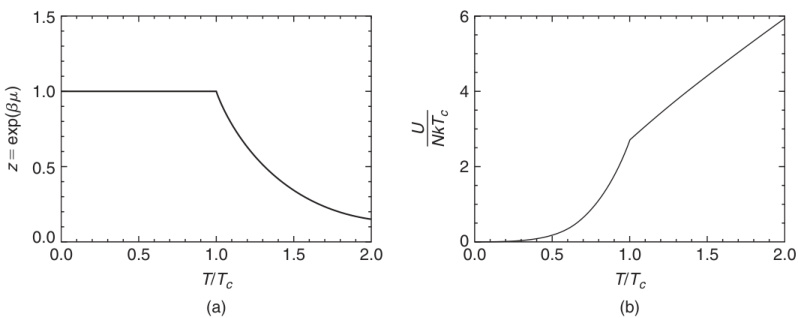
\includegraphics[width=0.71\textwidth]{images/chap7_m802e402f4dec0efe551279e739e9dda7.jpg}
\caption{玻色-爱因斯坦凝聚体在谐振子阱中的 fugacity（a）及缩放温度（\(T/T_c\)）对应的缩放内能（b）。}
\label{fig:7_7.10}
\end{figure}
\begin{figure}[htbp]
\centering
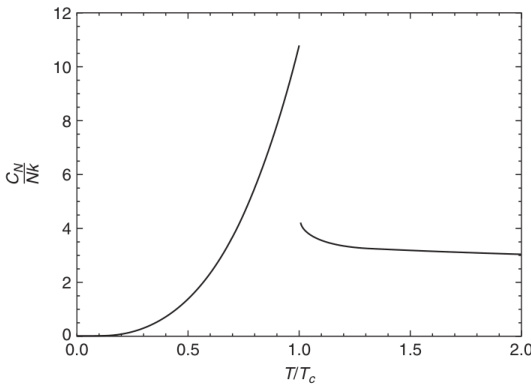
\includegraphics[width=0.47\textwidth]{images/chap7_m5300bbc7a332be8d089e1e5225afc117.jpg}
\caption{玻色-爱因斯坦凝聚体在谐振子阱中的缩放比热随缩放温度（\(T/T_c\)）的变化。}
\label{fig:7_7.11}
\end{figure}
图~\ref{fig:7_7.12} 展示了\(^{87}\)Rb玻色-爱因斯坦凝聚体内能的实验数据。斜率的断裂表明比热具有不连续性。当然，在具有有限粒子数的系统中，所有与相变相关的非解析性都已消除。当 \(N\) 为有限值时，凝聚体分数会平滑地趋近于零，从而使得热容中的不连续性被平滑化。Pathria（1998）推导出了依赖于 \(N\) 的温度标记，这些标记能够根据凝聚体分数和比热来指示玻色-爱因斯坦凝聚的开始；另请参阅Kirsten和Toms（1996）以及Haugerud、Haugest和Ravndal（1997）。
\begin{figure}[htbp]
\centering
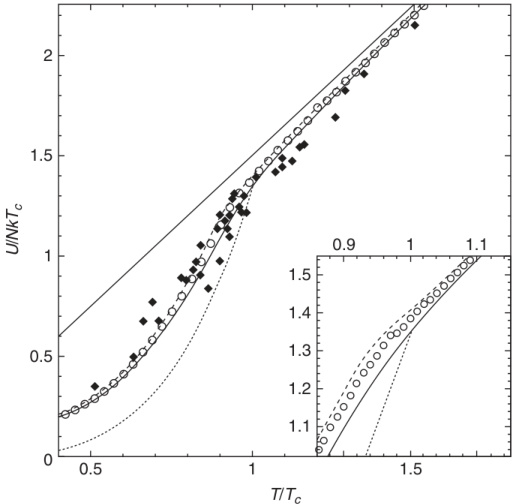
\includegraphics[width=0.46\textwidth]{images/chap7_mfe2d1ae5d5360a08547054f200053320.jpg}
\caption{实验测量值与理论曲线的对比，插图给出临界温度附近放大图。}
\label{fig:7_7.12}
\end{figure}
\section{黑体辐射的热力学}\label{sec:7_3_blackbody}
玻色-爱因斯坦统计学最重要的应用之一，是用于研究黑体辐射的平衡性质。我们考虑一个体积为 \(V\) 的辐射腔，其温度为 \(T\)。从历史上看，该系统一直从两个几乎完全相同但概念上却截然不同的视角加以研究：
\begin{enumerate}
\item 作为由谐振子组成的系统，其能量为量子化的，即 \((n_s+\frac{1}{2})\hbar\omega_s\)，其中 \(n_s=0,1,2,\ldots\)，\(\omega_s\) 是某一谐振子的角频率；
\item 作为由相同且无法区分的量子，即所谓的光子，构成的气体，光子的能量（对应于辐射模式的频率 \(\omega_s\)）为 \(\hbar\omega_s\)。
\end{enumerate}
第一种观点本质上是普朗克在1900年所采用的观点，只不过我们在此还加入了谐振子的零点能；对于辐射的热力学而言，这一能量并不重要，完全可以完全忽略。由于各谐振子彼此可区分（仅凭 \(\omega_{s}\) 的不同值），它们将遵循麦克斯韦-玻尔兹曼统计；然而，单个谐振子的配分函数 \(Q_{1}(V,T)\) 的表达式会与经典表达式有所不同，因为此时谐振子所能达到的能量是离散的，而非连续的；请参阅式（3.8.2） 和 式（3.8.14）。因此，一个频率为 \(\omega_{s}\) 的普朗克谐振子的能量期望值由式（3.8.20） 给出，不包括零点项 \(\frac{1}{2}\hbar\omega_{s}\)：
\begin{equation}\tag{7.2.11}\label{eq:7.2.11}
\langle \varepsilon _ { s } \rangle = \frac { \hbar \omega _ { s } } { e ^{\hbar \omega _ { s} / k T } - 1 } .
\end{equation}
现在，腔体单位体积内，在频率范围 \((\omega, \omega + d\omega)\) 内的正常振动模的数量，由瑞利公式给出
\begin{equation}\tag{7.2.12}\label{eq:7.2.12}
2 \cdot 4 \pi \left( \frac { 1 } { \lambda } \right) ^{2} d \left( \frac { 1 } { \lambda } \right) = \frac { \omega ^{2} d \omega } { \pi ^{2} c ^{3} } ,
\end{equation}
其中已加入因子 2，以考虑横模式的双重性；\(^{11}\) 此处的符号 \(c\) 表示光速。根据\autoref{eq:7.2.11}和\autoref{eq:7.2.12}，与频率范围 \((\omega, \omega + d\omega)\) 相关的能量密度由以下公式给出
\begin{equation}\tag{7.2.13}\label{eq:7.2.13}
u ( \omega ) d \omega = \frac { \hbar } { \pi ^{2} c ^{3} } \, \frac { \omega ^{3} d \omega } { e ^{\hbar \omega / k T} - 1 } ,
\end{equation}
这正是普朗克关于黑体光谱中能量分布的"公式"。通过对 (3) 进行对所有 \(\omega\) 值的积分，我们得到腔体中的总能量密度。
第二种观点源于玻色（1924年）和爱因斯坦（1924年、1925年）。玻色研究了"光子在各个能级间的分布"这一问题；然而，他并没有专注于对各类光子的分配
与其像通常那样将光子分配到各个能级上，他更关注的是能级本身的统计规律！他探讨了诸如"某个能级 \(\varepsilon_{s}=(\hbar\omega_{s})\) 在某一时刻被 \(n_{s}\) 个光子占据的概率"、"\(n_{s}\) 和 \(\varepsilon_{s}\) 的平均值"等问题。实际上，能级的统计规律确实是玻尔兹曼式的；然而，\(n_{s}\) 和 \(\varepsilon_{s}\) 的平均值却会发现
\begin{equation}\tag{7.2.14}\label{eq:7.2.14}
\begin{array}{r} { \langle n _ { s } \rangle = \displaystyle \sum _ { n _ { s } = 0 } ^{\infty} n _ { s } e ^{- n _ { s} \hbar \omega _ { s } / k T } \Bigg / \displaystyle \sum _ { n _ { s } = 0 } ^{\infty} e ^{- n _ { s} \hbar \omega _ { s } / k T } } \\{ = \displaystyle \frac { 1 } { e ^{\hbar \omega _ { s} / k T } - 1 } } \end{array}
\end{equation}
因此，
\begin{equation}\tag{7.2.15}\label{eq:7.2.15}
\langle \varepsilon _ { s } \rangle = \hbar \omega _ { s } \langle n _ { s } \rangle = \frac { \hbar \omega _ { s } } { e ^{\hbar \omega _ { s} / k T } - { \bf 1 } } ,
\end{equation}
与我们先前的结论\autoref{eq:7.2.11}完全一致。为了求得动量介于 \(\hbar\omega/c\) 与 \(\hbar(\omega+d\omega)/c\) 之间的光子态数，玻色借助了这一数与"相空间中相关区域的体积"之间的联系，其结果为
\begin{equation}\tag{7.2.16}\label{eq:7.2.16}
g ( \omega ) d \omega \approx 2 \cdot \frac { V } { h ^{3} } \left\{ 4 \pi \left( \frac { \hbar \omega } { c } \right) ^{2} \left( \frac { \hbar d \omega } { c } \right) \right\} = \frac { V \omega ^{2} d \omega } { \pi ^{2} c ^{3} } ,
\end{equation}
这也与我们先前的结论\autoref{eq:7.2.12}完全一致。因此，他最终得到了普朗克分布公式。需要指出的是，尽管重点在于其他方面，但引导玻色得出最终结果的数学步骤，与振子方法中的步骤在本质上是完全平行的！
另一方面，爱因斯坦更深入地探究了这一问题，并从整体上对光子与能级的统计特性进行了思考。他从玻色的处理方式中推断出：在将光子分配到各个能级的过程中，必须牢记的一个基本事实是：光子彼此无法区分——而这一事实在玻色的处理中早已被隐含地考虑在内。爱因斯坦对所需分布的推导，基本上与第6.1节所给出的推导相同，仅有一个重要区别：由于任意给定体积内的光子总数是不确定的，因此不再存在"固定 N"这一约束条件。由此，拉格朗日乘数 \(\alpha\) 并未参与讨论，也因此，\(\langle n_{\varepsilon} \rangle\) 的最终公式变得更加简洁：
\begin{equation}\tag{7.2.17}\label{eq:7.2.17}
\langle n _ { \varepsilon } \rangle = \frac { 1 } { e ^{\varepsilon / k T} - 1 } ;
\end{equation}
与式（6.1.18a）或（6.2.22）进行比较。上述结果与式（4）完全一致，其中 \(\varepsilon = \hbar\omega_{s}\)。爱因斯坦的后续推导步骤与玻色的推导过程完全相同。
其中
\begin{equation}\tag{7.2.18}\label{eq:7.2.18}
u ^{\prime} ( x ) = \frac { \pi ^{2} \hbar ^{3} c ^{3} } { ( k T ) ^{4} } u ( x )  \mathrm { a n d }  x = \frac { \hbar \omega } { k T } .
\end{equation}
对于长波长情况（\(x \ll 1\)），公式（8）可简化为瑞利（1900年）和詹森（1905年）的经典近似，即\(^{14}\)
\begin{equation}\tag{7.2.19}\label{eq:7.2.19}
u ^{\prime} ( x ) \approx x ^{2} ,
\end{equation}
对于短波长情况（\(x \gg 1\)），其可简化为维恩在1896年提出的著名公式，即
\begin{equation}\tag{7.2.20}\label{eq:7.2.20}
u ^{\prime} ( x ) \approx x ^{3} e ^{- x} .
\end{equation}
与标准的玻色-爱因斯坦结果\autoref{eq:7.1.2}相比，\autoref{eq:7.2.17}表明，我们所面对的情况中，\(z\) 正好等于1。不难看出，这主要是因为本题中粒子的总数量是无限的。因此，它们的平衡数 \(\overline{N}\) 必须由这样一条条件来确定：系统的自由能达到最小值，即 \(\{(\partial A/\partial N)_{N=\overline{N}}\}_{V,T}=0\)。根据定义，这一条件意味着 \(\mu=0\)，从而 \(z=1\)。
若将 \(\langle\varepsilon_{s}\rangle\) 的值采用等分能量的量子理论值（1）而非量子理论值，那么瑞利-詹森公式便能直接推导出来。
为了便于比较，图中还加入了极限形式（10）和（11）。值得注意的是，普朗克曲线与维恩曲线下的面积分别约为 \(\pi^{4}/15 (\simeq 6.49)\) 和 6。然而，瑞利-詹森曲线却饱受高频灾难之苦！
对于腔体内的总能量密度，我们可从方程（8）和（9）中得出
\begin{equation}\tag{7.2.21}\label{eq:7.2.21}
\begin{array}{r} { \frac { U } { V } = \int _ { 0 } ^{\infty} u ( x ) d x = \frac { ( k T ) ^{4} } { \pi ^{2} \hbar ^{3} c ^{3} } \int _ { 0 } ^{\infty} \frac { x ^{3} d x } { e ^{x} - 1 } } \\{ = \frac { \pi ^{2} k ^{4} } { 15 \hbar ^{3} c ^{3} } T ^{4} . } \end{array}
\end{equation}
如果腔体壁上存在一个微小的开口，光子便会"逸出"通过该开口。单位开口面积上的辐射净流速可由下式给出，详见方程（6.4.12），
\begin{equation}\tag{7.2.22}\label{eq:7.2.22}
\frac { 1 } { 4 } \frac { U } { V } c = \frac { \pi ^{2} k ^{4} } { 60 \hbar ^{3} c ^{2} } T ^{4} = \sigma T ^{4} ,
\end{equation}
其中
\begin{equation}\tag{7.2.23}\label{eq:7.2.23}
\sigma = \frac { \pi ^{2} k ^{4} } { 60 \hbar ^{3} c ^{2} } = 5 . 67 0 \times 10 ^{- 8} \mathrm { W m ^{- 2} K ^{- 4} } .
\end{equation}
\autoref{eq:7.2.23}描述了黑体辐射的斯特藩-玻尔兹曼定律，\(\sigma\) 为斯特藩常数。该定律最早由斯特藩于1879年基于实验观测得出；五年后，玻尔兹曼则从热力学角度对其进行了推导。
为进一步研究热力学，我们对光子气体的巨配分函数进行了计算。利用方程（6.2.17），并设 \(z=1\)，我们得到
\begin{equation}\tag{7.2.24}\label{eq:7.2.24}
\ln \mathcal { Q } ( V , T ) \equiv \frac { P V } { k T } = - \sum _ { \varepsilon } \ln ( 1 - e ^{- \varepsilon / k T} ) .
\end{equation}
将求和替换为积分，并借助极端相对论公式
\begin{equation}\tag{7.2.25}\label{eq:7.2.25}
a ( \varepsilon ) d \varepsilon = 2 V \frac { 4 \pi p ^{2} d p } { h ^{3} } = \frac { 8 \pi V } { h ^{3} c ^{3} } \varepsilon ^{2} d \varepsilon ,
\end{equation}
经过部分积分后，我们得到
\begin{equation}\tag{7.2.26}\label{eq:7.2.26}
\ln \mathcal { Q } ( V , T ) \equiv \frac { P V } { k T } = \frac { 8 \pi V } { 3 h ^{3} c ^{3} } \frac { 1 } { k T } \int _ { 0 } ^{\infty} \frac { \varepsilon ^{3} d \varepsilon } { e ^{\varepsilon / k T} - 1 } .
\end{equation}
这里，我们利用了定积分的值为 \(6\zeta(4)=\pi^{4}/15\) 的事实；详情请参见附录D。
通过变量替换，此式变为
\begin{equation}\tag{7.2.27}\label{eq:7.2.27}
\begin{array}{r} { P V = \frac { 8 \pi V } { 3 h ^{3} c ^{3} } ( k T ) ^{4} \int _ { 0 } ^{\infty} \frac { x ^{3} d x } { e ^{x} - 1 } } \\{ = \frac { 8 \pi ^{5} V } { 45 h ^{3} c ^{3} } ( k T ) ^{4} = \frac { 1 } { 3 } U . } \end{array}
\end{equation}
由此我们得到了辐射理论中广为人知的结果——辐射的压力等于其能量密度的三分之一；另请参阅方程（6.4.3）和（6.4.4）。接下来，由于系统的化学势为零，亥姆霍兹自由能等于 \(-PV\)；因此
\begin{equation}\tag{7.2.28}\label{eq:7.2.28}
A = - P V = - { \frac { 1 } { 3 } } U ,
\end{equation}
其中
\begin{equation}\tag{7.2.29}\label{eq:7.2.29}
S \equiv { \frac { U - A } { T } } = { \frac { 4 } { 3 } } { \frac { U } { T } } \propto V T ^{3}
\end{equation}
并且
\begin{equation}\tag{7.2.30}\label{eq:7.2.30}
C _ { V } = T \biggl ( \frac { \partial S } { \partial T } \biggr ) _ { V } = 3 S .
\end{equation}
若辐射经历可逆绝热变化，那么\(T\)与\(V\)的变化规律将遵循如下公式（19），
\begin{equation}\tag{7.2.31}\label{eq:7.2.31}
V T ^{3} = \mathrm { c o n s t . }
\end{equation}
将（21）与\(P \propto T^{4}\)这一事实相结合，我们得到该系统的绝热线方程，即
\begin{equation}\tag{7.2.32}\label{eq:7.2.32}
P V ^{4 / 3} = \mathrm { c o n s t . }
\end{equation}
然而，需要注意的是，光子气体的比值\(C_{P}/C_{V}\)并非4/3；它实际上是无穷大！最后，我们推导出了辐射腔中光子平衡数\(\overline{N}\)的表达式。我们得到
\begin{equation}\tag{7.2.33}\label{eq:7.2.33}
\begin{array}{r} { \overline { { N } } = \frac { V } { \pi ^{2} c ^{3} } \int _ { 0 } ^{\infty} \frac { \omega ^{2} d \omega } { e ^{\hbar \omega / k T} - 1 } } \\{ = V \frac { 2 \zeta ( 3 ) ( k T ) ^{3} } { \pi ^{2} h ^{3} c ^{3} } \propto V T ^{3} . } \end{array}
\end{equation}
尽管该公式颇具启发性，但其不应被简单地视为理所当然，因为在本问题中，由变量\(N\)的波动幅度——而该波动幅度由\((\partial P/\partial V)^{-1}\)这一量决定——是无限大的；参见方程（4.5.7）。
黑体辐射最重要的例子之一便是2.7K的宇宙微波背景辐射，它是大爆炸遗留下来的残余。方程（12）和（23）在我们理解早期宇宙的热力学过程方面发挥着重要作用；请参阅问题7.24以及第九章。
\section{声波领域}\label{ux58f0ux6ce2ux9886ux57df}
与第7.3节所讨论的问题在数学上颇为相似的问题，源于宏观物体——尤其是固体——的振动模式。与黑体辐射的情况类似，固体振动模式的问题同样可以分别从将系统视为谐振子集合，或将其视为一个封闭区域、其中包含声量子气体——即所谓的声子——的角度来加以研究。为了说明这一点，我们以一个由\(N\)个原子构成的经典固体为例，这些原子在空间中的位置由坐标\((x_1, x_2, \ldots, x_{3N})\)来确定。在最低能量状态中，这些坐标的值可表示为\((\overline{x}_1, \overline{x}_2, \ldots, \overline{x}_{3N})\)。将原子偏离其平衡位置的位移\((x_i - \overline{x}_i)\)用变量\(\xi_i (i = 1, 2, \ldots, 3N)\)来表示，则系统在配置\((x_i)\)下的动能可表示为
\begin{equation}\tag{7.4.1}\label{eq:7.4.1}
K = \frac { 1 } { 2 } m \sum _ { i = 1 } ^{3 N} \dot { x } _ { i } ^{2} = \frac { 1 } { 2 } m \sum _ { i = 1 } ^{3 N} \dot { \xi } _ { i } ^{2} ,
\end{equation}
并由势能表示为
\begin{equation}\tag{7.4.2}\label{eq:7.4.2}
\begin{array}{rl} { \Phi \equiv \Phi ( x _ { i } ) = \Phi ( \overline { { x } } _ { i } ) + \sum _ { i } \bigg ( \frac { \partial \Phi } { \partial x _ { i } } \bigg ) _ { ( x _ { i } ) = ( \overline { { x } } _ { i } ) } ( x _ { i } - \overline { { x } } _ { i } ) } & { } \\{ + \sum _ { i , j } \frac { 1 } { 2 } \bigg ( \frac { \partial ^{2} \Phi } { \partial x _ { i } \partial x _ { j } } \bigg ) _ { ( x _ { i } ) = ( \overline { { x } } _ { i } ) } ( x _ { i } - \overline { { x } } _ { i } ) ( x _ { j } - \overline { { x } } _ { j } ) + \cdots . } & { } \end{array}
\end{equation}
本展开式中的主项表示在所有原子均处于其平均位置\(\bar{x}_{i}\)且静止时，固体所具有的（最小）能量；该能量可记作\(\Phi_{0}\)。接下来的项因函数\(\Phi(x_{i})\)在\((x_{i})=(\bar{x}_{i})\)处取得极小值，因此其一阶导数在该点为零，故各项均为零。展开式的二阶项代表了原子围绕其平均位置振动的谐振分量。若我们假设这些振动的总体振幅并不大，则可仅保留展开式的谐振项，而忽略后续的各项；此时我们便处于所谓的谐振近似之中。由此，我们可以写出
\begin{equation}\tag{7.4.3}\label{eq:7.4.3}
H = \Phi _ { 0 } + \left\{ \sum _ { i } \frac { 1 } { 2 } m \dot { \xi } _ { i } ^{2} + \sum _ { i , j } \alpha _ { i j } \dot { \xi } _ { i } \dot { \xi } _ { j } \right\} ,
\end{equation}
其中
\begin{equation}\tag{7.4.4}\label{eq:7.4.4}
\alpha _ { i j } = \frac { 1 } { 2 } \left( \frac { \partial ^{2} \Phi } { \partial x _ { i } \partial x _ { j } } \right) _ { ( x _ { i } ) = ( \overline { { x } } _ { i } ) } .
\end{equation}
现在我们引入一种线性变换，将坐标\(\xi_{i}\)转换为所谓的正则坐标\(q_{i}\)，并选择变换矩阵，使得哈密顿量的新表达式中不包含任何交叉项，即，
\begin{equation}\tag{7.4.5}\label{eq:7.4.5}
H = \Phi _ { 0 } + \sum _ { i } \frac { 1 } { 2 } m \Big ( \dot { q } _ { i } ^{2} + \omega _ { i } ^{2} q _ { i } ^{2} \Big ) ,
\end{equation}
其中\(\omega_{i}(i=1,2,\ldots,3N)\)是系统的正则模态的特征频率，其本质上由\(\alpha_{ij}\)这一参数决定，或者进一步由势能函数\(\Phi(x_{i})\)的性质所决定。\autoref{eq:7.4.5}表明，固体的能量在\((最小)\)值\(\Phi_{0}\)之外的部分，可以被视为由一组\(3N\)个一维、非相互作用、谐振子所构成，而这些谐振子的特征频率\(\omega_{i}\)则由系统内的原子间相互作用决定。
从经典力学的角度来看，\(3N\)个正则模态对应于晶格的一种畸变波，亦即声波。而在量子力学中，这些模态会激发出称为声子的量子，其产生方式与电磁场的振动模态激发光子的方式大致相同。然而，两者之间存在一个重要的区别：对于电磁场而言，其正则模态的数量是无限的；而对于固体而言，正则模态的数量（或声子能级的数量）则由晶格位点的数量所限定。这使得声场的热力学行为与辐射场的热力学行为呈现出一定的差异；不过，在低温条件下，当固体的高频模态不太可能被激发时，这些差异便变得微不足道，我们最终会发现，这两组结果之间存在着惊人的相似性。
如今，固体的热力学研究可以沿第3.8节的思路展开。首先，我们注意到哈密顿量(5)的特征值为
\begin{equation}\tag{7.4.6}\label{eq:7.4.6}
E \{ n _ { i } \} = \Phi _ { 0 } + \sum _ { i } \Big ( n _ { i } + \frac { 1 } { 2 } \Big ) \hbar \omega _ { i } ,
\end{equation}
其中，各振子的"激发态"数值 \(n_{i}\) 表示了系统中各振子的"激发态"（或 equivalently，表示系统中各声子能级的占据数）。系统的内能则可表示为
\begin{equation}\tag{7.4.7}\label{eq:7.4.7}
U ( T ) = \left\{ \Phi _ { 0 } + \sum _ { i } \frac { 1 } { 2 } \hbar \omega _ { i } \right\} + \sum _ { i } \frac { \hbar \omega _ { i } } { e ^{\hbar \omega _ { i} / k T } - 1 } .
\end{equation}
当然，声子本身的数量是无限的。因此，声子气体的化学势也为零。
括号内的表达式给出了在绝对零度下固体的能量。项 \(\Phi_{0}\) 为负值，且其大小远大于振子的总零点能——\(\sum_{i\frac{1}{2}}\hbar\omega_{i}\)——二者共同决定了晶格的结合能。\autoref{eq:7.4.7} 中的最后一项代表了能量中随温度变化的部分，\(^{17}\) 这一项决定了固体的比热：
\begin{equation}\tag{7.4.8}\label{eq:7.4.8}
C _ { V } ( T ) \equiv \left( \frac { \partial U } { \partial T } \right) _ { V } = k \sum _ { i } \frac { ( \hbar \omega _ { i } / k T ) ^{2} e ^{\hbar \omega _ { i} / k T } } { ( e ^{\hbar \omega _ { i} / k T } - 1 ) ^{2} } .
\end{equation}
要进一步推进研究，我们需要了解固体的频率谱。要从基本原理出发获得这一频谱并非易事。因此，我们通常通过实验来获取该频谱，或者基于对频谱的某些合理假设来进行推导。爱因斯坦率先将量子概念应用于固体理论（1907年），为了简化起见，他假设所有频率 \(\omega_{i}\) 都相等。将这一（普遍）值记作 \(\omega_{E}\)，固体的比热可表示为
\begin{equation}\tag{7.4.9}\label{eq:7.4.9}
C _ { V } ( T ) = 3 N k E ( x ) ,
\end{equation}
其中，\(E(x)\) 即所谓的爱因斯坦函数：
\begin{equation}\tag{7.4.10}\label{eq:7.4.10}
E ( x ) = \frac { x ^{2} e ^{x} } { ( e ^{x} - 1 ) ^{2} } ,
\end{equation}
其中
\begin{equation}\tag{7.4.11}\label{eq:7.4.11}
x = \hbar \omega _ { E } / k T = \Theta _ { E } / T .
\end{equation}
图~7.14 中的虚线曲线展示了比热随温度的变化情况，其依据为爱因斯坦公式\autoref{eq:7.4.9}。在温度足够高的情况下，即 \(T \gg \Theta_E\)，因而 \(x \ll 1\) 时，爱因斯坦的结果趋于经典结果，即 \(3Nk\)。而在温度足够低的情况下，即 \(T \ll \Theta_E\)，因而 \(x \gg 1\) 时，比热会以指数级的速度下降，并随着 \(T \to 0\) 而趋近于零。然而，根据理论计算所得的下降速率，与实际观测到的下降速率相比显得过快。尽管如此，爱因斯坦的方法至少为理解固体比热偏离经典杜朗-佩蒂定律提供了理论基础——按照该定律，\(C_V = 3R \simeq 5.96\) 卡路里每摩尔每摄氏度。
另一方面，德拜（1912年）则允许存在连续的频率谱，并将其上限设定为 \(\omega_{D}\)，使得振动正常模式的总数为 \(3N\)。
其中，\(g(\omega)d\omega\) 表示频率位于区间 \((\omega, \omega + d\omega)\) 内的正常振动模式的数量。对于 \(g(\omega)\)，德拜采用了瑞利公式（7.3.2），并对其进行了修正，以适应所研究的问题。设 \(c_L\) 为纵波传播速度，\(c_T\) 为横波传播速度（并注意到，对于任意频率 \(\omega\)，横波模式均为双重简并），则方程（12）变为
\begin{equation}\tag{7.4.12}\label{eq:7.4.12}
\int _ { 0 } ^{\omega D} V \left( \frac { \omega ^{2} d \omega } { 2 \pi ^{2} c _ { L } ^{3} } + \frac { \omega ^{2} d \omega } { \pi ^{2} c _ { T } ^{3} } \right) = 3 N ,
\end{equation}
由此可得截止频率
\begin{equation}\tag{7.4.13}\label{eq:7.4.13}
\omega _ { D } ^{3} = 18 \pi ^{2} \frac { N } { V } \left( \frac { 1 } { c _ { L } ^{3} } + \frac { 2 } { c _ { T } ^{3} } \right) ^{- 1} .
\end{equation}
因此，德拜谱可以写成
\begin{equation}\tag{7.4.14}\label{eq:7.4.14}
g ( \omega ) = \left\{ \begin{array}{ll} { \displaystyle \frac { 9 N } { \omega _ { D } ^{3} } \omega ^{2} } & { \mathrm { f o r ~ } \omega \leq \omega _ { D } , } \\{ 0 } & { \mathrm { f o r ~ } \omega > \omega _ { D } . } \end{array} \right.
\end{equation}
在进一步依据德拜谱计算固体比热之前，我们似乎有必要先作两点说明。首先，德拜谱只是对固体中实际现象的一种理想化描述；例如，它可以与图~7.15 所示的典型谱进行比较。尽管对于低频模式（即所谓的声学模式），德拜近似是合理的，但在高频模式（即所谓的光学模式）的情况下，却出现了严重的偏差。在\ldots\ldots{}
无论如何，对于诸如比热等"平均"量而言，谱的精细细节并不十分重要。其次，固体的纵波模式和横波模式应各自拥有各自的截止频率，例如 \(\omega_{D,L}\) 和 \(\omega_{D,T}\)，而非采用统一的截止频率 \(\omega_{D}\)，原因很简单：在晶格的 \(3N\) 个正常模式中，恰好有 \(N\) 个是纵波模式，而 \(2N\) 个是横波模式。因此，我们应当采用的公式并非（13），
\begin{equation}\tag{7.4.15}\label{eq:7.4.15}
\int _ { 0 } ^{\omega _ { D , L} } V \frac { \omega ^{2} d \omega } { 2 \pi ^{2} c _ { L } ^{3} } = N  \mathrm { a n d }  \int _ { 0 } ^{\omega _ { D , T} } V \frac { \omega ^{2} d \omega } { \pi ^{2} c _ { T } ^{3} } = 2 N .
\end{equation}
我们注意到，这两个截止频率对应于共同的波长 \(\lambda_{\mathrm{min}} = \left( \frac{4\pi V}{3N} \right)^{1/3}\)，这一波长与固体中的平均原子间距离相当。这是相当合理的，因为当波长短于 \(\lambda_{\mathrm{min}}\) 时，若再谈论原子位移的波，就显得有些无意义了。
在德拜近似下，\autoref{eq:7.4.8}给出
\begin{equation}\tag{7.4.16}\label{eq:7.4.16}
C _ { V } ( T ) = 3 N k D ( x _ { 0 } ) ,
\end{equation}
其中 \(D(x_0)\) 是所谓的德拜函数：
\begin{equation}\tag{7.4.17}\label{eq:7.4.17}
D ( x _ { 0 } ) = \frac { 3 } { x _ { 0 } ^{3} } \int _ { 0 } ^{x _ { 0} } \frac { x ^{4} e ^{x} d x } { ( e ^{x} - 1 ) ^{2} } ,
\end{equation}
其中
\begin{equation}\tag{7.4.18}\label{eq:7.4.18}
x _ { 0 } = \frac { \hbar \omega _ { D } } { k T } = \frac { \Theta _ { D } } { T } ,
\end{equation}
\(\Theta_{D}\) 即为固体的所谓德拜温度。通过分部积分，德拜函数的表达式变为
\begin{equation}\tag{7.4.19}\label{eq:7.4.19}
D ( x _ { 0 } ) = - \frac { 3 x _ { 0 } } { e ^{x _ { 0} } - 1 } + \frac { 12 } { x _ { 0 } ^{3} } \int _ { 0 } ^{x _ { 0} } \frac { x ^{3} d x } { e ^{x} - 1 } .
\end{equation}
对于 \(T \gg \Theta_{D}\)，即 \(x_{0} \ll 1\) 的情形，函数 \(D(x_{0})\) 可以表示为 \(x_{0}\) 的幂级数：
\begin{equation}\tag{7.4.20}\label{eq:7.4.20}
D ( x _ { 0 } ) = 1 - { \frac { x _ { 0 } ^{2} } { 20 } } + \cdots .
\end{equation}
因此，当 \(T \to \infty\) 时，\(C_V \to 3Nk\)；此外，根据这一理论，只要 \(T > 3\Theta_D\)，经典结果就应能适用于误差不超过 \(\frac{1}{2}\)\% 的范围。而对于 \(T \ll \Theta_D\)，即 \(x_0 \gg 1\) 的情形，函数 \(D(x_0)\) 可以写成：
\begin{equation}\tag{7.4.21}\label{eq:7.4.21}
\begin{array}{r} { D ( x _ { 0 } ) = \frac { 12 } { x _ { 0 } ^{3} } \int _ { 0 } ^{\infty} \frac { x ^{3} d x } { e ^{x} - 1 } + O ( e ^{- x _ { 0} } ) , } \\{ \approx \frac { 4 \pi ^{4} } { 5 x _ { 0 } ^{3} } = \frac { 4 \pi ^{4} } { 5 } \left( \frac { T } { \Theta _ { D } } \right) ^{3} . } \end{array}
\end{equation}
因此，在低温下，固体的比热遵循德拜 \(T^{3}\) 定律：
\begin{equation}\tag{7.4.22}\label{eq:7.4.22}
C _ { V } = \frac { 12 \pi ^{4} } { 5 } N k \biggl ( \frac { T } { \Theta _ { D } } \biggr ) ^{3} = 46 4 . 4 \biggl ( \frac { T } { \Theta _ { D } } \biggr ) ^{3} \mathrm { c a l \ m o l e } ^{- 1} \mathrm { K } ^{- 1} .
\end{equation}
从\autoref{eq:7.4.22}中可以清楚地看出，对固体进行低温比热测量，不仅能够验证 \(T^{3}\) 定律的正确性，还能获得德拜温度 \(\Theta_{D}\) 的经验值。19 德拜温度 \(\Theta_{D}\) 的数值，也可以通过已知参数 \(N/V\)、\(c_{L}\) 和 \(c_{T}\) 来计算出截止频率 \(\omega_{D}\)；具体见式（14）和式（19）。这些估算值之间的高度吻合，进一步证明了德拜理论的合理性。一旦得知 \(\Theta_{D}\) 的值，便可通过利用表格中列出的函数 \(D(x_{0})\) 的数值，从理论上覆盖整个温度范围。20 一个典型的例子已在图~7.14 中展示过。我们发现，不仅在低温下 \(T^{3}\) 定律依然成立，而且在整个观测范围内，理论与实验之间的拟合度都相当理想。
19 可以证明，根据这一理论，在 \(T < \Theta_{D}/10\) 的范围内，偏离 \(T^{3}\) 定律的幅度不应超过 2\%。然而，对于金属而言，我们无法期待真正达到 \(T^{3}\) 区域，因为早在该区域之前，电子气体的比热就可能成为主导贡献因素（参见第 8.3 节）；除非将这两种贡献区分开来，否则我们很可能会从这些观测中得到一个略显被抑制的 \(\Theta_{D}\) 值。
20 例如，请参阅 Fowler 和 Guggenheim（1960，第 144 页）。
作为低温区域一致性的一个又一例证，我们在此附上另一幅图——图~7.16，该图基于在低于 5K 温度下使用 KCl 晶体所获得的数据；请参阅 Keesom 和 Pearlman（1953）。图中，\(C_{V}/T\) 的观测值被绘制于 \(T^{2}\) 坐标系中。显然，这些数据很好地落在一条直线上，而通过该直线的斜率，便可确定 \(\Theta_{D}\) 的值。因此，对于 KCl，我们得到 \(\Theta_{D} = 233 \pm 3\)K，这一结果与各处相关弹性常数估计值所得到的 230 至 246 K 值基本一致。
在表 7.1 中，我们列出了若干晶体的 \(\Theta_{D}\) 值，这些值分别来自比热测量以及弹性常数的测定结果。
一般来说，如果某一特定系统的比热测量结果符合 \(T^3\) 规律，那么可以推断该系统中的热激发完全由声子所负责。我们同样预期，在液体中也会发生类似的现象，但存在两个重要的差异。首先，由于液体无法承受剪切应力，因此无法维持横向振动模式；因此，由 \(N\) 个原子组成的液体，仅具有 \(N\) 个纵向振动模式。其次，液体的正常模式并不一定严格呈谐振状态；因此，除了声子之外，我们还可能遇到其他类型的激发，例如涡流流动或湍流（甚至还有某种改良型的激发，如液态氦 \(^{4}\) 中的罗通子）。
其中，
\begin{equation}\tag{7.4.23}\label{eq:7.4.23}
\omega _ { D } = \left( \frac { 6 \pi ^{2} N } { V } \right) ^{1 / 3} c ,
\end{equation}
\(c\) 为液体中的声速。液体单位质量的比热则可表示为
\begin{equation}\tag{7.4.24}\label{eq:7.4.24}
c _ { V } = \frac { 2 \pi ^{2} k ^{4} } { 15 \rho \hbar ^{3} c ^{3} } T ^{3} ,
\end{equation}
其中，\(\rho\) 为质量密度。将 \(\rho = 0.1455\,\mathrm{g/cm}^3\) 和 \(c = 238\,\mathrm{m/s}\) 代入，上述结果变为
\begin{equation}\tag{7.4.25}\label{eq:7.4.25}
c _ { V } = 0 . 02 09 T ^{3} \mathrm { j o u l e g } ^{- 1} \mathrm { K } ^{- 1} .
\end{equation}
Wiebes 等人（1957）在 \(0 < T < 0.6\)K 时的实验测量结果，均符合以下表达式
\begin{equation}\tag{7.4.26}\label{eq:7.4.26}
c _ { V } = ( 0 . 02 04 \pm 0 . 00 04 ) T ^{3} \mathrm { j o u l e g } ^{- 1} \mathrm { K } ^{- 1} .
\end{equation}
理论结果与实验观测之间的吻合度显然相当高。
\section{声场的惯性密度}\label{ux58f0ux573aux7684ux60efux6027ux5bc6ux5ea6}
为了进一步理解液态氦\(^{4}\)的低温行为，我们对处于热平衡状态的声子气体所对应的"惯性质量"进行了测定。为此，我们以"处于质量运动中的声子气体"为研究对象；通过确定该气体的动量\(P\)与质量运动速度\(\nu\)之间的关系，我们便能轻松地计算出所要研究的这一性质。由于系统中声子的总数是不确定的，因此问题并不受固定\(N\)的约束；相应地，未定乘数\(\alpha\)可以被取为零。然而，我们如今又为系统新增了一项约束条件——即总动量\(P\)的固定，除此之外，
总能量\(E\)的固定约束。在这些约束条件下，声子能级\(\varepsilon(\boldsymbol{p})\)的平均占据数将为
\begin{equation}\tag{7.5.1}\label{eq:7.5.1}
\langle n ( p ) \rangle = \frac { 1 } { \exp ( \beta \varepsilon + \gamma \cdot p ) - 1 } .
\end{equation}
如同往常一样，参数\(\beta\)等于\(1/kT\)。为了确定\(\gamma\)，我们似乎自然地选择评估气体的漂移速度。若以质量运动方向为z轴，则漂移速度的大小\(\nu\)可由"单个声子速度中\(u_z\)分量的平均值"给出：
\begin{equation}\tag{7.5.2}\label{eq:7.5.2}
\nu = \langle u \cos \theta \rangle .
\end{equation}
现在，对于声子而言，
\begin{equation}\tag{7.5.3}\label{eq:7.5.3}
\varepsilon = p c  \mathrm { a n d }  u \equiv \frac { d \varepsilon } { d p } = c ,
\end{equation}
其中\(c\)为介质中的声速。此外，出于对称性的考虑，我们预期未定向量\(\boldsymbol{\gamma}\)要么与质量运动方向平行，要么与之反平行；因此，我们可以写成
\begin{equation}\tag{7.5.4}\label{eq:7.5.4}
\gamma \cdot p = \gamma _ { z } p _ { z } = \gamma _ { z } p \cos \theta .
\end{equation}
鉴于\autoref{eq:7.5.1}、\autoref{eq:7.5.3}和\autoref{eq:7.5.4}，\autoref{eq:7.5.2}变为
\begin{equation}\tag{7.5.5}\label{eq:7.5.5}
\nu = \frac { \int _ { 0 } ^{\infty} \int _ { 0 } ^{\pi} [ \exp \{ \beta p c ( 1 + ( \gamma _ { z } / \beta c ) \cos \theta ) \} - 1 ] ^{- 1} ( c \cos \theta ) ( p ^{2} d p 2 \pi \sin \theta d \theta ) } { \int _ { 0 } ^{\infty} \int _ { 0 } ^{\pi} [ \exp \{ \beta p c ( 1 + ( \gamma _ { z } / \beta c ) \cos \theta ) \} - 1 ] ^{- 1} ( p ^{2} d p 2 \pi \sin \theta d \theta ) } .
\end{equation}
进行替换
\begin{equation}\tag{7.5.6}\label{eq:7.5.6}
\cos \theta = \eta ,  p ( { \bf 1 } + ( \gamma _ { z } / \beta c ) \eta ) = p ^{\prime}
\end{equation}
并消去对\(p'\)的积分，我们得到
\begin{equation}\tag{7.5.7}\label{eq:7.5.7}
\nu = c \frac { \int _ { - 1 } ^{1} ( 1 + ( \gamma _ { z } / \beta c ) \eta ) ^{- 3} \eta d \eta } { \int _ { - 1 } ^{1} ( 1 + ( \gamma _ { z } / \beta c ) \eta ) ^{- 3} d \eta } = - \gamma _ { z } / \beta .
\end{equation}
由此可知，
\begin{equation}\tag{7.5.8}\label{eq:7.5.8}
\gamma = - \beta v .
\end{equation}
据此，平均占据数的表达式变为
\begin{equation}\tag{7.5.9}\label{eq:7.5.9}
\langle n ( p ) \rangle = \frac { 1 } { \exp \{ \beta ( \varepsilon - v \cdot p ) \} - 1 } .
\end{equation}
将\autoref{eq:7.5.9}与气体静止参考系中的对应结果进行比较，即
\begin{equation}\tag{7.5.10}\label{eq:7.5.10}
\langle n _ { 0 } ( p _ { 0 } ) \rangle = \frac { 1 } { \exp ( \beta \varepsilon _ { 0 } ) - 1 } ,
\end{equation}
可以看出，通过施加质量运动对系统造成的改变，不过是两种参考系之间伽利略变换的直观体现。
或者，\autoref{eq:7.5.9}也可以写成
\begin{equation}\tag{7.5.11}\label{eq:7.5.11}
\langle n ( p ) \rangle = \frac { 1 } { \exp ( \beta p ^{\prime} c ) - 1 } = \frac { 1 } { \exp \{ \beta p c ( 1 - ( \nu / c ) \cos \theta ) \} - 1 } .
\end{equation}
因此，\autoref{eq:7.5.9}对漂移速度\(\nu\)作出了严格的限制——即，\(\nu\)不得超过声子的速度\(c\)，否则部分占据数将变为负值！事实上，正如我们后续的分析所表明的那样，当\(\nu\)接近\(c\)时，本节所建立的理论框架将失效。因此，声子气体的流动速度\(c\)可被视为临界速度：
\begin{equation}\tag{7.5.12}\label{eq:7.5.12}
( \nu _ { c } ) _ { \mathrm { p h } } = c .
\end{equation}
这一结果与液氦II超流性问题之间的关联将在下一部分中得到阐明。
接下来，我们计算声子气体的总动量\(P\)：
\begin{equation}\tag{7.5.13}\label{eq:7.5.13}
P = \sum _ { p } \langle n ( p ) \rangle p .
\end{equation}
事实上，向量\(P\)将与向量\(v\)平行，而后者本身已沿\(z\)轴方向运动。因此，我们只需计算动量的\(z\)分量：
\begin{equation}\tag{7.5.14}\label{eq:7.5.14}
\begin{aligned} P & = P _ { z } = \sum _ { p } \langle n ( p ) \rangle p _ { z } \\& = \int _ { 0 } ^{\infty} \int _ { 0 } ^{\pi} \frac { p \cos \theta } { \exp \{ \beta p c ( 1 - ( v / c ) \cos \theta ) \} } - 1 \left( \frac { V p ^{2} d p 2 \pi \sin \theta d \theta } { h ^{3} } \right) \\& = \frac { 2 \pi V } { h ^{3} } \int _ { 0 } ^{\infty} \frac { p ^{\prime 3} d p ^{\prime} } { \exp ( \beta p ^{\prime} c ) - 1 } \int _ { 0 } ^{\pi} \{ 1 - ( v / c ) \cos \theta \} ^{- 4} \cos \theta \sin \theta d \theta \\& = V \frac { 16 \pi ^{5} } { 45 h ^{3} c ^{3} \beta ^{4} } \cdot \frac { v / c ^{2} } { ( 1 - v ^{2} / c ^{2} ) ^{3} } . \end{aligned}
\end{equation}
气体的总能量\(E\)由以下公式给出：
\begin{equation}\tag{7.5.15}\label{eq:7.5.15}
\begin{array}{rl} & { E = \sum _ { p } \langle n ( p ) \rangle p c } \\& {  = \frac { 2 \pi \, V c } { h ^{3} } \int _ { 0 } ^{\infty} \frac { p ^{\prime 3} \, d p ^{\prime} } { \exp ( \beta p ^{\prime} c ) - 1 } \int _ { 0 } ^{\pi} \{ 1 - ( v / c ) \cos \theta \} ^{- 4} \sin \theta d \theta } \\& {  = V \frac { 4 \pi ^{5} } { 15 h ^{3} c ^{3} \beta ^{4} } \frac { 1 + \frac { 1 } { 3 } v ^{2} / c ^{2} } { ( 1 - v ^{2} / c ^{2} ) ^{3} } . } \end{array}
\end{equation}
自然地，我们将\(P/\nu\)的比值视为声子气体的"惯性质量"。相应地，其质量密度\(\rho\)则由以下公式给出：
\begin{equation}\tag{7.5.16}\label{eq:7.5.16}
\rho = \frac { P } { v V } = \frac { 16 \pi ^{5} k ^{4} T ^{4} } { 45 h ^{3} c ^{5} } \frac { 1 } { ( 1 - v ^{2} / c ^{2} ) ^{3} } .
\end{equation}
对于\((v/c) \ll 1\)的情况——通常情况下确实如此——声子气体的质量密度可表示为：
\begin{equation}\tag{7.5.17}\label{eq:7.5.17}
( \rho _ { 0 } ) _ { \mathrm { p h } } = \frac { 16 \pi ^{5} k ^{4} } { 45 h ^{3} c ^{5} } T ^{4} = \frac { 4 } { 3 c ^{2} } ( E _ { 0 } / V ) .
\end{equation}
将液氦\(^{4}\)在低温下的声子质量密度代入公式，该质量密度相对于液体的实际密度而言，可表示为：
\begin{equation}\tag{7.5.18}\label{eq:7.5.18}
( \rho _ { 0 } ) \mathrm { p h } / \rho _ { \mathrm { H e } } = 1 . 22 \times 10 ^{- 4} T ^{4} ;
\end{equation}
例如，在\(T=0.3\mathrm{K}\)时，这一比值约为\(9.9\times10^{-7}\)。而在如\(0.3\mathrm{K}\)这样的温度下，声子是液氦\(^{4}\)中唯一需要考虑的激发态；因此，计算所得的结果应与"液态正常流体的密度\(\rho_{n}\)与液态总密度\(\rho\)之比"相对应。要直接精确地确定如此微小的比值几乎是不可能的；然而，借助其他实验上可行的液体性质进行间接估算，却为上述结果提供了有力的证实——详见图~7.17。
第7.6节 液氦II中的基本激发态
朗道（1941年、1947年）提出了一套简单的理论框架，能够较好地解释液氦II在低温下、且未过于靠近\(\lambda\)点时的行为。根据这一框架，液态被视作一个弱激发的量子力学系统，在该系统中，从基态（\(T = 0\mathrm{K}\)）出发的偏离，可通过"悬浮于静止背景之上的基本激发态气体"来加以描述。激发态气体对应于"正常流体"，而静止背景则代表"超流体"。
因此，在\(T=T_{\lambda}\)时，\(\rho_{n}=\rho_{\mathrm{He}}\)，而\(\rho_{s}=0\)。当\(T>T_{\lambda}\)时，液体在各方面都表现为普通流体，即我们通常所熟知的液态氦I。
基于纯粹的经验性考量，朗道还提出了液态氦II中基本激发态的能量-动量关系\(\varepsilon(p)\)。在低动量下，\(\varepsilon\)与\(p\)之间的关系呈线性（这正是声子的典型特征），而在高动量下，则呈现出非单调的特性。这些激发态被假定为玻色子，并且在低温下（此时激发态的数量并不算多）彼此之间互不相互作用；随后，通过采用一种简单直接的统计力学方法，便可计算出液体的宏观性质。研究发现，朗道的理论能够相当成功地解释液态氦II在约0至2K温度范围内的观测性质；然而，仍需进一步验证，液体中的实际激发态是否真的符合所提出的能量谱。
在科恩和费曼（1957年）的建议指导下，多位实验工作者着手通过散射长波长中子（\(\lambda \gtrsim 4\text{\AA}\)）来研究液态氦II中的激发态能谱。在低于2K的温度下，最重要的散射过程是中子在液体中产生单个激发态的过程。通过测量在某一角度\(\phi\)下散射的中子的修正波长\(\lambda_{f}\)，便可以确定在散射过程中产生的激发态的能量\(\varepsilon\)和动量\(p\)。
可根据相关守恒定律加以确定：
\begin{equation}\tag{7.5.19}\label{eq:7.5.19}
\varepsilon = h ^{2} ( \lambda _ { i } ^{- 2} - \lambda _ { f } ^{- 2} ) / 2 m ,
\end{equation}
\begin{equation}\tag{7.5.20}\label{eq:7.5.20}
p ^{2} = h ^{2} ( \lambda _ { i } ^{- 2} + \lambda _ { f } ^{- 2} - 2 \lambda _ { i } ^{- 1} \lambda _ { f } ^{- 1} \cos \phi ) ,
\end{equation}
其中\(\lambda_{i}\)为中子的初始波长，\(m\)为中子质量。通过改变\(\phi\)，或\(\lambda_{i}\)，便可绘制出激发态的完整能谱。
首次沿着这一方向展开的全面研究由亚内尔等人（1959年）完成；他们的研究成果如图~7.18所示，与朗道所提出的经验能谱有着惊人的相似之处。在1.1K温度下获得的能谱中，较为重要的特征如下：
（i）如果我们对位于 \(p/\hbar = 0.55\text{\AA}^{-1}\) 周围的点拟合线性、类声子谱（\(\varepsilon = pc\)），则可得 \(c\) 的值为 \((239 \pm 5)\,\mathrm{m/s}\)，这一结果与液体中声速的实测值——约 \(238\,\mathrm{m/s}\)——高度吻合。
（ii）该谱在 \(\varepsilon/k = (13.92 \pm 0.10)\text{\AA}^{-1}\) 处通过一个最大值。
（iii）随后，在 \(p/\hbar = (1.92 \pm 0.01)\text{\AA}^{-1}\) 处出现一个最小值，其邻近区域可由朗道的罗通能谱来描述：
\begin{equation}\tag{7.5.21}\label{eq:7.5.21}
\varepsilon ( p ) = \Delta + \frac { ( p - p _ { 0 } ) ^{2} } { 2 \mu } ,
\end{equation}
与
\begin{equation}\tag{7.5.22}\label{eq:7.5.22}
\begin{array}{r} { \Delta / k = ( 8 . 65 \pm 0 . 04 ) \mathrm { K } , } \\{ p _ { 0 } / \hbar = ( 1 . 92 \pm 0 . 01 ) \text { \AA } ^{- 1} , } \end{array}
\end{equation}
以及
\begin{equation}\tag{7.5.23}\label{eq:7.5.23}
\mu = ( 0 . 16 \pm 0 . 01 ) m _ { \mathrm { H e } } .
\end{equation}
（iv）在 \(p/\hbar \simeq 2.18\text{\AA}^{-1}\) 以上，谱线呈线性上升，且斜率仍为 \(c\)。我们还分别在1.6K和1.8K的温度下获得了数据。发现该谱的总体形状与1.1K时基本一致；仅 \(\Delta\) 的数值略低一些。
在后续研究中，Henshaw 和 Woods（1961）将观测范围扩展到了谱线两端；他们的研究成果见图~7.19。在谱线的较低端，他们将测量范围一直延伸至 \(p/\hbar = 0.26\text{\AA}^{-1}\)，并发现实验所得的
\^{}\{21\}"罗通"这一术语是朗道提出的，他最初认为这些激发态或许能在某种程度上代表液体中一种旋转性质的局域扰动。然而，后续的理论研究，尤其是费曼（1953、1954）以及布鲁克纳和泽瓦达（1957）的研究，并未支持这一观点。尽管如此，"罗通"这一术语仍被沿用至今。
这些点确实位于一条直线上（斜率为237 m/s）。在谱线的较高端，他们将测量范围进一步拓展至 \(p/\hbar=2.68\text{\AA}^{-1}\)，并发现：在经过1.91\(\text{\AA}^{-1}\) 处的最小值后，曲线以不断增大的斜率向上延伸，直至大约2.4\(\text{\AA}^{-1}\)，此时二阶导数 \(\partial^2\varepsilon/\partial p^2\) 发生符号反转；曲线随后的趋势表明，谱线中可能存在第二个最大值！22
要对液氦II的热力学性质进行评估，我们首先注意到，在温度足够低的情况下，我们仅存在一些低能激发态，即声子。液态的热力学行为随后由第7.4节和第7.5节中推导出的公式所支配。当温度高于约0.5K时，第二类激发态——即罗通子（其动量接近\(p_0\)）——也会出现。在0.5K与约1K之间，液态的行为由声子与罗通子共同决定。然而，当温度高于1K时，声子对液态各项热力学性质的贡献已变得相当微弱；此时，只有罗通子需要被纳入考量。
接下来，我们将研究罗通子对液态各项热力学性质的温度依赖性。鉴于能谱具有连续性，人们自然会预期，如同声子一样，罗通子也遵循玻色-爱因斯坦统计。此外，系统中罗通子的总数量\(N\)是相当不确定的；因此，它们的化学势\(\mu\)恒为零。于是，我们得到罗通子的平均占据数为：
\begin{equation}\tag{7.5.24}\label{eq:7.5.24}
\langle n ( p ) \rangle = \frac { 1 } { \exp \{ \beta \varepsilon ( p ) \} - 1 } ,
\end{equation}
其中，\(\varepsilon(p)\)由\autoref{eq:7.5.4}和\autoref{eq:7.5.5}给出。在所有我们所关心的温度下（即\(T \leq 2\)K），项\(\exp\{\beta\varepsilon(p)\}\)的最小值——即\(\exp(\Delta/kT)\)——远远大于1。因此，我们可以写成：
\begin{equation}\tag{7.5.25}\label{eq:7.5.25}
\langle n ( p ) \rangle \simeq \exp \{ - \beta \varepsilon ( p ) \} .
\end{equation}
因此，罗通子系统的\(q\)势可表示为：
\begin{equation}\tag{7.5.26}\label{eq:7.5.26}
q ( V , T ) \equiv \frac { P V } { k T } = - \sum _ { p } \ln [ 1 - \exp \{ - \beta \varepsilon ( p ) \} ] \simeq \sum _ { p } \exp \{ - \beta \varepsilon ( p ) \} \simeq \overline { { { N } } } ,
\end{equation}
其中，\(\overline{N}\)为系统中"平衡"状态下的罗通子数量。对\(p\)的求和可以替换为积分，其结果为：
\begin{equation}\tag{7.5.27}\label{eq:7.5.27}
\frac { P V } { k T } = \overline { { N } } = \frac { V } { h ^{3} } \int _ { 0 } ^{\infty} e ^{- \left\{ \Delta + \frac { ( p - p _ { 0} ) ^{2} } { 2 \mu } \right\} } \Bigg / k T _ { ( 4 \pi p ^{2} d p ) } .
\end{equation}
\^{}\{22\} 这一结果似乎印证了皮塔耶夫斯基（1959）的一项重要预言：光谱的端点可能出现在一个"临界"激发动量值\(p_{c}\)处，此时\(\varepsilon_{c}\)等于\(2\Delta\)，且\((\partial\varepsilon/\partial p)_{c}\)为零。
将\(p = p_0 + (2\mu kT)^{1/2}x\)代入，我们得到：
\begin{equation}\tag{7.5.28}\label{eq:7.5.28}
\frac { P V } { k T } = \overline { { { N } } } = \frac { 4 \pi p _ { 0 } ^{2} V } { h ^{3} } e ^{- \Delta / k T} ( 2 \mu k T ) ^{1 / 2} \int e ^{- x ^ { 2} } \left\{ 1 + \frac { ( 2 \mu k T ) ^{1 / 2} } { p _ { 0 } } x \right\} ^{2} d x .
\end{equation}
使该积分产生显著贡献的变量 \(x\) 的“相关”范围，大致围绕 \(x=0\) 这一数值呈对称分布；因此，被积函数中线性项的净效应几乎可以忽略不计。二次项同样不重要，因为其系数 \((2\mu kT)/p_{0}^{2}\) 远小于 1。因此，我们只需考虑 \(\exp(-x^{2})\) 的积分。显然，我们可以轻松验证：该积分的上下限恰好使得在不影响积分值的前提下，我们可以将积分上限和下限分别取为 \(-\infty\) 和 \(+\infty\)；此时，积分的值便简单地为 \(\pi^{1/2}\)。由此我们得到：
\begin{equation}\tag{7.5.29}\label{eq:7.5.29}
\frac { P V } { k T } = \overline { { N } } = \frac { 4 \pi p _ { 0 } ^{2} V } { h ^{3} } ( 2 \pi \mu k T ) ^{1 / 2} e ^{- \Delta / k T} .
\end{equation}
罗顿气体的自由能由下式给出（由于\(\mu = 0\)）
\begin{equation}\tag{7.5.30}\label{eq:7.5.30}
A = - P V = - \overline { { { N } } } k T \propto T ^{3 / 2} e ^{- \Delta / k T} ,
\end{equation}
由此可得
\begin{equation}\tag{7.5.31}\label{eq:7.5.31}
\begin{array}{rlr} & { } & { S = - \left( \frac { \partial A } { \partial T } \right) _ { V } = - A \left\{ \frac { 3 } { 2 T } + \frac { \Delta } { k T ^{2} } \right\} = \overline { { N } } k \left\{ \frac { 3 } { 2 } + \frac { \Delta } { k T } \right\} , } \\& { } & { U = A + T S = \overline { { N } } \left( \Delta + \frac { 1 } { 2 } k T \right) } \end{array}
\end{equation}
并且
\begin{equation}\tag{7.5.32}\label{eq:7.5.32}
C _ { V } = \left( \frac { \partial \, U } { \partial \, T } \right) _ { V } = \overline { { { N } } } k \left\{ \frac { 3 } { 4 } + \frac { \Delta } { k T } + \left( \frac { \Delta } { k T } \right) ^{2} \right\} .
\end{equation}
显然，当\(T \rightarrow 0\)时，这些结果均趋近于零（本质上呈指数级衰减）。
现在我们来确定罗顿气体的惯性质量密度。按照第7.5节的步骤，对于能量谱为\(\varepsilon(p)\)的激发态气体，我们得到：
\begin{equation}\tag{7.5.33}\label{eq:7.5.33}
\rho _ { 0 } = \frac { M _ { 0 } } { V } = \operatorname* { l i m } _ { \nu \to 0 } \frac { 1 } { \nu } \int n ( \varepsilon - \nu \cdot p ) p \frac { d ^{3} p } { h ^{3} } ,
\end{equation}
\^{}\{23\}回顾积分\autoref{eq:7.5.9}，我们在此所做的工作，实际上就是将被积函数中的\(p^{2}\)替换为其平均值\(p_{0}^{2}\)，然后对变量\((p-p_{0})\)进行完整范围内的积分。
\^{}\{24\}这一结果极具启发性：对于罗顿而言，只存在一个真正的自由度——即罗顿动量的大小——而这一自由度在热力学上是有效的！
其中，\(n(\varepsilon - \boldsymbol{v} \cdot \boldsymbol{p})\)表示状态\(\varepsilon(p)\)的平均占据数，该数值是在以参考系\(K\)为基准、且气体以漂移速度\(\boldsymbol{v}\)作质量运动的参考系中所观测到的。25 对于小的\(\nu\)，函数\(n(\varepsilon - \boldsymbol{v} \cdot \boldsymbol{p})\)可以按泰勒级数展开为\(\boldsymbol{v}\)的多项式，仅保留其中的项\(n(\varepsilon) - (\boldsymbol{v} \cdot \boldsymbol{p})\partial n(\varepsilon)/\partial \varepsilon\)。对前一部分的积分表示系统在静止参考系\(K_0\)中所观测到的动量密度，且其值为零。因此，我们最终得到：
\begin{equation}\tag{7.5.34}\label{eq:7.5.34}
\begin{array}{r} { \rho _ { 0 } = - \frac { 1 } { h ^{3} } \int p ^{2} \cos ^{2} \theta \frac { \partial n ( \varepsilon ) } { \partial \varepsilon } ( p ^{2} d p 2 \pi \sin \theta d \theta ) } \\{ = - \frac { 4 \pi } { 3 h ^{3} } \int _ { 0 } ^{\infty} \frac { \partial n ( \varepsilon ) } { \partial \varepsilon } p ^{4} d p , } \end{array}
\end{equation}
这一结果适用于任意能量谱以及任意统计分布。
对于声子，我们得到
\begin{equation}\tag{7.5.35}\label{eq:7.5.35}
\begin{array}{rl} & { ( \rho _ { 0 } ) _ { \mathrm { p h } } = - \frac { 4 \pi } { 3 h ^{3} c } \int _ { 0 } ^{\infty} \frac { d n ( p ) } { d p } p ^{4} d p } \\& {  = - \frac { 4 \pi } { 3 h ^{3} c } \left[ n ( p ) \cdot p ^{4} \Big | _ { 0 } ^{\infty} - \int _ { 0 } ^{\infty} n ( p ) \cdot 4 p ^{3} d p \right] } \\& {  = \frac { 4 } { 3 c ^{2} } \int _ { 0 } ^{\infty} n ( p ) \cdot p c \left( \frac { 4 \pi p ^{2} d p } { h ^{3} } \right) = \frac { 4 } { 3 c ^{2} } ( E _ { 0 } ) _ { \mathrm { p h } } / V , } \end{array}
\end{equation}
这一结果与我们先前得出的结论（7.5.15）完全一致。
对于罗顿，\(n(\varepsilon) \simeq \exp(-\beta \varepsilon)\)；因此，\(\partial n(\varepsilon)/\partial \varepsilon \simeq -\beta n(\varepsilon)\)。据此，根据\autoref{eq:7.5.17}，
\begin{equation}\tag{7.5.36}\label{eq:7.5.36}
\begin{array}{rl} & { ( \rho _ { 0 } ) _ { \mathrm { r o t } } = \frac { 4 \pi \beta } { 3 \hbar ^{3} } \int n ( \varepsilon ) p ^{4} d p } \\& {  = \frac { \beta } { 3 } \, \langle p ^{2} \rangle \frac { \overline { { N } } } { V } \simeq \frac { p _ { 0 } ^{2} } { 3 k T } \frac { \overline { { N } } } { V } } \\& {  = \frac { 4 \pi p _ { 0 } ^{4} } { 3 \hbar ^{3} } \left( \frac { 2 \pi \mu } { k T } \right) ^{1 / 2} e ^{- \Delta / k T} , } \end{array}
\end{equation}
在极低温度下（\(T < 0.3\)K），罗顿对流体惯性的贡献相较于声子贡献几乎可以忽略不计。而在相对较高的温度下（\(T \sim 0.6\)K），这两种贡献开始趋于相当。当温度高于1 K时，罗顿的贡献远超声子的贡献；在这样的温度下，仅凭罗顿密度就足以构成正常流体的密度\(\rho_{n}\)。
若能确定理论计算所得的密度 \(\rho_{n}\) 与液态氦的实际密度 \(\rho_{\mathrm{He}}\) 相等时的临界温度 \(T_{c}\)，将具有重要的启发意义；这将意味着液态氦中的超流成分将彻底消失（从而导致液态氦II向液态氦I的转变）。通过这一分析，我们得出 \(T_{c} \simeq 2.5 \mathrm{K}\)，而实验值 \(T_{\lambda}\) 则为 \(\simeq 2.19 \mathrm{K}\)。考虑到在本计算中，我们一直假设罗顿气体在过渡点之前始终处于非相互作用体系之中；事实上，由于在较高温度下存在数量极其庞大的激发态，这一假设已不再成立。
\autoref{eq:7.5.19}表明，一个罗顿激发体的等效质量为 \(p_{0}^{2}/3kT\)。从数值上看，这一质量大约是氦原子质量的 10 到 15 倍（因此，比罗顿能谱的参数 \(\mu\) 大了多个数量级）。然而，罗顿等效质量更重要的意义在于：它与罗顿气体的温度成反比！历史上，这一特性最早由朗道（1947 年）基于液态氦II中第二声速及其比热的实验数据，通过经验方法加以发现。如今，由于激发体的等效质量通常由 \(\langle p^{2}\rangle/3kT\) 这一量值决定，朗道推断出，该液体中相关激发体的 \(\langle p^{2}\rangle\) 量值必须与温度无关。因此，随着液体温度的升高，激发体的平均 \(p^{2}\) 值应保持不变；这一值可记作 \(p_{0}^{2}\)。另一方面，激发体的平均能量 \(\varepsilon\) 则会随温度升高而上升。要调和这两者之间的矛盾，唯一的途径便是引入一种非单调能谱，在 \(p=p_{0}\) 处出现最低点。
最后，我们想谈谈超流的临界速度问题。为此，我们考虑一个无激发态的超流体，其质量为 \(M\)，其动能 \(E\) 和动量 \(P\) 分别为 \(\frac{1}{2}Mv^2\) 和 \(Mv\)。这些量的变化之间存在如下关系：
\begin{equation}\tag{7.5.37}\label{eq:7.5.37}
\delta E = ( \pmb { v } \cdot \delta \mathbf { P } ) .
\end{equation}
假设这些变化是由流体中激发体 \(\varepsilon(\boldsymbol{p})\) 的产生所引起的，那么根据守恒定律，我们必然有：
\begin{equation}\tag{7.5.38}\label{eq:7.5.38}
\delta E = - \varepsilon  \mathrm { a n d }  \delta P = - p .
\end{equation}
\autoref{eq:7.5.21}和\autoref{eq:7.5.22}最终得出的结果是
\begin{equation}\tag{7.5.39}\label{eq:7.5.39}
\varepsilon = ( v \cdot p ) \leq v p .
\end{equation}
因此，除非流体的漂移速度 \(\nu\) 大于或至少等于 \((\varepsilon/p)\) 这一数值，否则无法在流体中产生激发 \(\varepsilon(p)\)。相应地，如果 \(\nu\) 甚至低于 \(\varepsilon/p\) 的最低值，流体中就根本无法产生任何激发，从而该流体将保持其超流特性。由此我们得到了一条维持超流状态的条件：
\begin{equation}\tag{7.5.40}\label{eq:7.5.40}
\nu < \nu _ { c } = ( \varepsilon / p ) _ { \mathrm { m i n } } ,
\end{equation}
这一现象被称为朗道超流准则。速度 \(v_{c}\) 被称为超流的临界速度；它标志着流体表现出超流行为时的"上限"流动速度。观测到的临界速度大小会因所采用的通道几何形状而有显著差异；通常情况下，通道越窄，临界速度越大。观测到的 \(v_{c}\) 值范围大约为 0.1 cm/s 至约 70 cm/s。
对 \(\nu_{c}\) 的理论估算显然极具研究价值。一方面，我们发现，如果激发遵循理想气体的关系式，即 \(\varepsilon=p^{2}/2m\)，那么临界速度竟然恰好为零。此时，任意速度 \(\nu\) 都大于临界速度；因此，完全不可能出现超流现象。这一结果意义重大，因为它清晰地揭示了这样一个事实：液体中的原子间相互作用——正是这些相互作用导致了与理想气体特征不同的激发谱——在促成超流现象的发生中起着至关重要的作用。由此可见，尽管理想玻色气确实会经历玻色-爱因斯坦凝聚现象，但它却无法自身支撑超流现象！另一方面，我们还发现：（i）对于声子，\(\nu_{c}=c\simeq2.4\times10^{4}\,\mathrm{cm/s}\)；（ii）对于罗通，\(\nu_{c}=\{(p_{0}^{2}+2\mu\Delta)^{1/2}-p_{0}\}/\mu\simeq\Delta/p_{0}\simeq6.3\times10^{3}\,\mathrm{cm/s}\)，这些数值与观测到的 \(\nu_{c}\) 值相比显得过高。事实上，液氦 II 中还存在另一种类型的集体激发，即量子化涡旋环，其能量-动量关系可表示为：\(\varepsilon\propto p^{1/2}\)。这些涡旋环的形成临界速度在数值上与实验结果基本吻合；不仅如此，\(\nu_{c}\) 随通道几何形状的变化规律，也可以通过涡旋环的尺寸来加以理解。
有关这一主题的综述，尤其是费曼的贡献，可参见 Mehra 和 Pathria（1994）；此外，本书第 11.4 节至第 11.6 节亦可作参考。
在氦-4的固态相中，也观察到了量子化、无耗散的玻色流。这种"超流体"行为由Kim和Chan（2004a、2004b）通过使用一种扭转振子来观测——该振子中填充了含有原子级孔洞的固态氦，并注入了二氧化硅。在P=60 atm时，当温度低于175 mK时，扭转频率会骤然升高。这些作者将这一结果解释为：处于孔隙中的固态氦原子能够自由流动，且几乎不产生耗散。
\section{问题}\label{ux95eeux9898_chap7}
7.1. 通过考虑占据数\(\langle n_{\varepsilon}\rangle\)的量级，证明在第7.1节的最终结果中，无论我们将和\autoref{eq:7.1.2}中有限个\((\varepsilon\neq0)\)项与\autoref{eq:7.1.6}中的\((\varepsilon=0)\)部分合并，还是将其纳入对\(\varepsilon\)的积分之中，都无关紧要。
7.2. 从\autoref{eq:7.1.7} 和 \autoref{eq:7.1.8}推导出维里展开\autoref{eq:7.1.13}，并验证所引用的维里系数数值。
7.3. 将\autoref{eq:7.1.24} 和 \autoref{eq:7.1.26}结合，并利用附录D中公式(D.9)的前两项，证明随着温度T从上方逐渐接近Tc，理想玻色气体的参数\(\alpha=(−lnz)\)将呈现出如下形式：
\begin{equation}\tag{7.5.41}\label{eq:7.5.41}
\alpha \approx \frac { 1 } { \pi } \left( \frac { 3 \zeta ( 3 / 2 ) } { 4 } \right) ^{2} \left( \frac { T - T _ { c } } { T _ { c } } \right) ^{2} .
\end{equation}
7.4. 证明对于理想玻色气体，
\begin{equation}\tag{7.5.42}\label{eq:7.5.42}
\frac { 1 } { z } \left( \frac { \partial z } { \partial T } \right) _ { P } = - \frac { 5 } { 2 T } \frac { g _ { 5 / 2 } ( z ) } { g _ { 3 / 2 } ( z ) } ;
\end{equation}
将此结果与\autoref{eq:7.1.36}进行比较。由此可得，
\begin{equation}\tag{7.5.43}\label{eq:7.5.43}
\gamma \equiv \frac { C _ { P } } { C _ { V } } = \frac { ( \partial z / \partial T ) _ { P } } { ( \partial z / \partial T ) _ { \nu } } = \frac { 5 } { 3 } \frac { g _ { 5 / 2 } ( z ) g _ { 1 / 2 } ( z ) } { \{ g _ { 3 / 2 } ( z ) \} ^{2} } ,
\end{equation}
正如\autoref{eq:7.1.48}中所描述的那样。请检查，当温度T从上方逐渐接近Tc时，\(\gamma\)和\(C_P\)均会以\((T - T_c)^{-1}\)的形式发散。
7.5. (a) 证明理想玻色气体的等温压缩率\(\kappa_{T}\)和绝热压缩率\(\kappa_{S}\)分别由以下公式给出：
\begin{equation}\tag{7.5.44}\label{eq:7.5.44}
\kappa T = \frac { 1 } { n k T } \frac { g _ { 1 / 2 } ( z ) } { g _ { 3 / 2 } ( z ) } ,  \kappa S = \frac { 3 } { 5 n k T } \frac { g _ { 3 / 2 } ( z ) } { g _ { 5 / 2 } ( z ) } ,
\end{equation}
其中\(n=(N/V)\)为气体中的粒子密度。请注意，当\(z\to0\)时，\(\kappa_T\)和\(\kappa_S\)将趋近于各自的经典值，即\(1/P\)和\(1/\gamma P\)。那么，当\(z\to1\)时，它们又将如何变化呢？
\begin{enumerate}
\def\labelenumi{(\alph{enumi})}
\setcounter{enumi}{1}
\item
  利用热力学关系
\end{enumerate}
\begin{equation}\tag{7.5.45}\label{eq:7.5.45}
C _ { P } - C _ { V } = T \left( \frac { \partial P } { \partial T } \right) _ { V } \left( \frac { \partial V } { \partial T } \right) _ { P } = T V _ { \kappa _ { T } } \left( \frac { \partial P } { \partial T } \right) _ { V } ^{2}
\end{equation}
以及
\begin{equation}\tag{7.5.46}\label{eq:7.5.46}
C _ { P } / C _ { V } = \kappa _ { T } / \kappa _ { S } ,
\end{equation}
推导出\autoref{eq:7.1.48} 和 \autoref{eq:7.1.48}。
7.6. 证明对于理想玻色气体，比热容\(C_V\)的温度导数可表示为
\begin{equation}\tag{7.5.47}\label{eq:7.5.47}
\frac { 1 } { N k } \left( \frac { \partial C _ { V } } { \partial T } \right) _ { V } = \left\{ \begin{array}{ll} { \frac { 1 } { T } \left[ \frac { 45 } { 8 } \frac { g _ { 5 / 2 } ( z ) } { g _ { 3 / 2 } ( z ) } - \frac { 9 } { 4 } \frac { g _ { 3 / 2 } ( z ) } { g _ { 1 / 2 } ( z ) } - \frac { 27 } { 8 } \frac { \{ g _ { 3 / 2 } ( z ) \} ^{2} g _ { - 1 / 2 } ( z ) } { \{ g _ { 1 / 2 } ( z ) \} ^{3} } \right] } & { \mathrm { f o r ~ } T > T _ { c } , } \\{ \frac { 45 } { 8 } \frac { \nu } { T \lambda ^{3} } \zeta \left( \frac { 5 } { 2 } \right) } & { \mathrm { f o r ~ } T < T _ { c } . } \end{array} \right.
\end{equation}
利用这些结果以及公式(D.9)中的主要项，验证\autoref{eq:7.1.38}。
7.7. 对理想玻色气体，计算并评估以下量值：\((\partial^2P/\partial T^2)_\nu\)、\((\partial^2\mu/\partial T^2)_\nu\) 和 \((\partial^2\mu/\partial T^2)_P\)，并检查您的结果是否满足热力学关系。
\begin{equation}\tag{7.5.48}\label{eq:7.5.48}
C _ { V } = V T \left( \frac { \partial ^{2} P } { \partial T ^{2} } \right) _ { \nu } - N T \left( \frac { \partial ^{2} \mu } { \partial T ^{2} } \right) _ { \nu } ,
\end{equation}
以及
\begin{equation}\tag{7.5.49}\label{eq:7.5.49}
C _ { P } = - N T \left( \frac { \partial ^{2} \mu } { \partial T ^{2} } \right) _ { P } .
\end{equation}
从上方和下方考察这些量在 \(T \rightarrow T_{c}\) 时的行为。
7.8. 流体中的声速由下式给出：
\begin{equation}\tag{7.5.50}\label{eq:7.5.50}
w = \sqrt { ( \partial P / \partial \rho ) _ { s } } ,
\end{equation}
其中，\(\rho\) 是流体的质量密度。证明对于理想玻色气体，
\begin{equation}\tag{7.5.51}\label{eq:7.5.51}
w ^{2} = \frac { 5 k T } { 3 m } \frac { g _ { 5 / 2 } ( z ) } { g _ { 3 / 2 } ( z ) } = \frac { 5 } { 9 } \langle u ^{2} \rangle ,
\end{equation}
其中，\(\langle u^{2}\rangle\) 是气体中粒子的平均平方速度。
7.9. 证明对于理想玻色气体，
\begin{equation}\tag{7.5.52}\label{eq:7.5.52}
\langle u \rangle \left\langle \frac { 1 } { u } \right\rangle = \frac { 4 } { \pi } \frac { g _ { 1 } ( z ) g _ { 2 } ( z ) } { \left\{ g _ { 3 / 2 } ( z ) \right\} ^{2} } ,
\end{equation}
\(u\) 为粒子的速度。考察并解释极限情况 \(z \rightarrow 0\) 和 \(z \rightarrow 1\)；与问题 6.6 进行比较。
7.10. 考虑在均匀重力场中、加速度为 \(g\) 的理想玻色气体。证明该气体中的玻色-爱因斯坦凝聚现象在温度 \(T_c\) 下发生，其值为
\begin{equation}\tag{7.5.53}\label{eq:7.5.53}
T _ { c } \simeq T _ { c } ^{0} \left[ 1 + \frac { 8 } { 9 } \frac { 1 } { \zeta \left( \frac { 3 } { 2 } \right) } \left( \frac { \pi m g L } { k T _ { c } ^{0} } \right) ^{1 / 2} \right] ,
\end{equation}
其中，\(L\) 为容器的高度，且 \(mgL \ll kT_{c}^{0}\)。同时证明，这里的凝聚现象伴随着气体比热容 \(C_{V}\) 的不连续性：
\begin{equation}\tag{7.5.54}\label{eq:7.5.54}
( \Delta C _ { V } ) _ { T = T _ { c } } \simeq - \frac { 9 } { 8 \pi } \, \zeta \left( \frac { 3 } { 2 } \right) N k \left( \frac { \pi \, m g L } { k T _ { c } ^{0} } \right) ^{1 / 2} \, ;
\end{equation}
参见 Eisenschitz（1958）。
7.11. 考虑由具有内部自由度的分子组成的理想玻色气体。假设除了基态 \(\varepsilon_0 = 0\) 外，仅需考虑内部能级谱的第一激发态 \(\varepsilon_1\)，求出该气体的凝聚温度 \(T_c\) 与 \(\varepsilon_1\) 的关系。证明当 \((\varepsilon_1/kT_c^0) \gg 1\) 时，
\begin{equation}\tag{7.5.55}\label{eq:7.5.55}
\frac { T _ { c } } { T _ { c } ^{0} } \simeq 1 - \frac { \frac { 2 } { 3 } } { \zeta \left( \frac { 3 } { 2 } \right) } e ^{- \varepsilon _ { 1} / k T _ { c } ^{0} }
\end{equation}
而当 \((\varepsilon_1/kT_c^0) \ll 1\) 时，
\begin{equation}\tag{7.5.56}\label{eq:7.5.56}
\frac { T _ { c } } { T _ { c } ^{0} } \simeq \left( \frac { 1 } { 2 } \right) ^{2 / 3} \left[ 1 + \frac { 2 ^{4 / 3} } { 3 \zeta \left( \frac { 3 } { 2 } \right) } \left( \frac { \pi \varepsilon _ { 1 } } { k T _ { c } ^{0} } \right) ^{1 / 2} \right] .
\end{equation}
【提示】要得到最后的结果，可利用附录 D 中公式 (D.9) 的前两项。
7.12. 考虑处于大正则系综中的理想玻色气体，并研究总粒子数 \(N\) 和总能量 \(E\) 的涨落。特别讨论当气体变得高度简并时的情形。
7.13. 考虑被限制在二维区域 \(A\) 内的理想玻色气体。用 \(z\)、\(T\) 和 \(A\) 表示激发态的粒子数 \(N_{e}\) 和基态的粒子数 \(N_{0}\)，并证明除非 \(T \rightarrow 0\)K，否则该系统不会出现玻色-爱因斯坦凝聚。
进一步完善你的论证，表明如果保持区域 \(A\) 和总粒子数 \(N\) 不变，同时要求 \(N_{e}\) 和 \(N_{0}\) 都达到 \(N\) 的数量级，则我们确实能够在以下条件下实现凝聚：
\begin{equation}\tag{7.5.57}\label{eq:7.5.57}
T \sim \frac { h ^{2} } { m k l ^{2} } \, \frac { 1 } { \ln N } ,
\end{equation}
其中，\(l[\sim\sqrt{(A/N)}]\) 表示系统中粒子间的平均距离。当然，若 \(A\) 和 \(N\) 都趋于无穷大，且保持 \(l\) 不变，则所求的 \(T\) 确实会趋近于零。
7.14. 考虑一个 \(n\) 维玻色气体，其单粒子能谱由 \(\varepsilon \propto p^{s}\) 给出，其中 \(s\) 为某一正数。讨论该系统中玻色-爱因斯坦凝聚的起始条件，尤其是其与 \(n\) 和 \(s\) 这两个参数之间的依赖关系。研究该系统的热力学行为，并证明，
\begin{equation}\tag{7.5.58}\label{eq:7.5.58}
P = \frac { s } { n } \frac { U } { V } ,  C _ { V } ( T \rightarrow \infty ) = \frac { n } { s } N k ,  \mathrm { a n d }  C _ { P } ( T \rightarrow \infty ) = \left( \frac { n } { s } + 1 \right) N k .
\end{equation}
7.15. 在 \(t=0\) 时，一维量子谐振子的基态波函数由以下公式给出：
\begin{equation}\tag{7.5.59}\label{eq:7.5.59}
\psi ( x , 0 ) = \frac { 1 } { \pi ^{1 / 4} \sqrt { a } } \exp \left( - \frac { x ^{2} } { 2 a ^{2} } \right) ,
\end{equation}
其中，\(a=\sqrt{\frac{\hbar}{m\omega_{0}}}\)。在 \(t=0\) 时，谐振子势被突然移除。利用波函数在 \(t=0\) 时的动量表示形式以及时间依赖的薛定谔方程，求解 \(t>0\) 时的空间波函数和密度；并与\autoref{eq:7.2.11} 进行对比。
7.16. 在 \(t=0\) 时，一组经典粒子处于温度 \(T\) 的平衡状态，其所处的三维谐振子势为 \(V(\boldsymbol{r})=\frac{1}{2}m\omega_{0}^{2}|\boldsymbol{r}|^{2}\)。在 \(t=0\) 时，谐振子势被突然移除。利用 \(t=0\) 时的动量分布，求解 \(t>0\) 时的空间密度。证明这一结果等价于\autoref{eq:7.2.15} 的高温极限情形。
7.17. 如第 7.1 节所示，\(n\lambda^{3}\) 是衡量系统量子性质的一个指标。利用\autoref{eq:7.2.11} 和\autoref{eq:7.2.15}，确定在 \(T=T_{c}/2\) 时，凝聚相与非凝聚相的谐振子阱中心处的 \(n\lambda^{3}\) 值。
7.18. 证明\autoref{eq:7.2.15} 中的半经典空间密度积分，能够正确地计数那些未凝聚到基态的原子数量。
7.19. 构建一种适用于各向同性二维阱中 \(N\) 个玻色子的理论。这种阱的特点是：沿 \(z\) 方向的激发所引起的能级间隔远大于其他方向上的能级间隔。求解该系统的态密度 \(a(\varepsilon)\)。在这种阱中是否能够形成玻色-爱因斯坦凝聚？如果可以，求出以阱频和 \(N\) 为变量的临界温度。要使系统表现出二维行为，第三方向的频率必须比原来高出多少？
7.20. 黑体辐射的（规范）配分函数可写为
\begin{equation}\tag{7.5.60}\label{eq:7.5.60}
Q ( V , T ) = \prod _ { \omega } Q _ { 1 } ( \omega , T ) ,
\end{equation}
从而
\begin{equation}\tag{7.5.61}\label{eq:7.5.61}
\ln Q ( V , T ) = \sum _ { \omega } \ln Q _ { 1 } ( \omega , T ) \approx \int _ { 0 } ^{\infty} \ln Q _ { 1 } ( \omega , T ) g ( \omega ) d \omega ;
\end{equation}
此处，\(Q_{1}(\omega,T)\) 是由式（3.8.14） 给出的单振子配分函数，而 \(g(\omega)\) 则是式（7.3.2） 所给出的状态密度。利用这些信息，计算系统的亥姆霍兹自由能，并推导出其他热力学性质，例如压力 \(P\) 以及（热）能量密度 \(U/V\)。将您的结果与第 7.3 节中基于系统 \(q\)-势所推导出的结果进行比较。
证明在黑体辐射腔中，每光子的平均能量几乎等于 \(2.7kT\)。
'22. 鉴于辐射场振动模式的频率 \(\omega\) 与体积之间的依赖关系，建立式（7.3.17） 中的压力 \(P\) 与能量密度 \(U/V\) 之间的关系。
7.23. 太阳可被视为温度为 5800K 的黑体。其直径约为 \(1.4 \times 10^{9}\) 米，而它与地球的距离约为 \(1.5 \times 10^{11}\) 米。
\begin{enumerate}
\def\labelenumi{(\alph{enumi})}
\item
  计算地球表面处太阳光的总辐射强度（单位：W/m²）。
\item
  若将一个完全吸收的表面置于太阳光线正对的位置，该表面将施加多大的压力？
\item
  如果一颗卫星上的平滑表面，面向太阳的一面，被视作理想的吸收体和发射体，那么它最终会达到怎样的平衡温度？
\end{enumerate}
7.24. 计算 2.725K 宇宙微波背景辐射的光子数密度、熵密度及能量密度。
7.25. 图~7.20 是一图，展示了固体的 \(C_{V}(T)\) 与 \(T\) 的关系；其中，极限值 \(C_{V}(\infty)\) 为经典结果 \(3Nk\)。请展示图中阴影区域，即
\begin{equation}\tag{7.5.62}\label{eq:7.5.62}
\int _ { 0 } ^{\infty} \{ C _ { V } ( \infty ) - C _ { V } ( T ) \} d T ,
\end{equation}
恰好等于该固体的零点能。从物理角度解释这一结果。
其中 \(x_{0,L} = (\hbar\omega_{D,L}/kT)\)，\(x_{0,T} = (\hbar\omega_{D,T}/kT)\)。将此结果与\autoref{eq:7.4.17}进行对比，并估算后者的误差性质及误差大小。
7.32. 由 \(n\) 个质量相同的物体（每个质量为 \(m\)）通过相同类型的弹簧（刚度为 \(K\)）沿直线连接而成的机械系统，其固有振动频率由以下公式给出：
\begin{equation}\tag{7.5.63}\label{eq:7.5.63}
\omega _ { r } = 2 \sqrt { \left( \frac { K } { m } \right) } \sin \left( \frac { r } { n } \cdot \frac { \pi } { 2 } \right) ; r = 1 , 2 , \ldots ( n - 1 ) .
\end{equation}
相应地，由 \(n\) 个相同原子构成的"线性"分子，可以被视为具有以下振动光谱：
\begin{equation}\tag{7.5.64}\label{eq:7.5.64}
\nu _ { r } = \nu _ { c } \sin \left( \frac { r } { n } \cdot \frac { \pi } { 2 } \right) ; r = 1 , 2 , \ldots ( n - 1 ) ,
\end{equation}
其中 \(\nu_{c}\) 是该分子的特征振动频率。证明：这一模型得出的分子振动比热随温度降低而呈 \(T^{1}\) 的变化规律，并在高温下趋于极限值 \((n-1)k\)。
7.33. 假设色散关系为 \(\omega = Ak^{s}\)，其中 \(\omega\) 为角频率，\(k\) 为固体中某振动模式的波数。证明：在低温下，该关系对固体比热的贡献与 \(T^{3/s}\) 成正比。
【注意，当 \(s=1\) 时，对应于晶格中弹性波的情况；而 \(s=2\) 则适用于在铁磁体系中传播的自旋波。】
7.34. 假设激发态为声子（\(\omega = Ak\)），证明其对 \(n\) 维德拜体系比热的贡献与 \(T^n\) 成正比。
【注意，硒和碲这两种元素形成的晶体中，原子链以平行方式排列，从某种意义上说，它们的行为类似于一维结构；因此，在一定温度范围内，\(T^1\) 定律依然适用。出于类似的原因，石墨在一定温度范围内也遵循 \(T^2\) 定律。】
7.35. 当固体的所有原子都"静止"于其平衡位置时，其（最小）势能可记作 \(\Phi_{0}(V)\)，其中 \(V\) 为固体的体积。同样地，振动的正常频率 \(\omega_{i}\)（\(i=1,2,\ldots,3N-6\)）可记作 \(\omega_{i}(V)\)。证明：该固体的压力由以下公式给出：
\begin{equation}\tag{7.5.65}\label{eq:7.5.65}
P = - \frac { \partial \Phi _ { 0 } } { \partial V } + \gamma \frac { U ^{\prime} } { V } ,
\end{equation}
其中，\(U'\) 为由原子振动所引起的固体内能，而 \(\gamma\) 为格鲁内伊森常数：
\begin{equation}\tag{7.5.66}\label{eq:7.5.66}
\gamma = - \frac { \partial \ln \omega } { \partial \ln V } \approx \frac { 1 } { 3 } .
\end{equation}
假设在 \(V \simeq V_0\) 的情况下，
\begin{equation}\tag{7.5.67}\label{eq:7.5.67}
\Phi _ { 0 } ( V ) = \frac { ( V - V _ { 0 } ) ^{2} } { 2 \kappa _ { 0 } V _ { 0 } } ,
\end{equation}
其中，\(\kappa_{0}\) 和 \(V_{0}\) 是常数，且 \(\kappa_{0}C_{V}T \ll V_{0}\)，请证明热膨胀系数（在恒压 \(P \simeq 0\) 下）可表示为
\begin{equation}\tag{7.5.68}\label{eq:7.5.68}
\alpha \equiv \frac { 1 } { V } \left( \frac { \partial V } { \partial T } \right) _ { N , P } = \frac { \gamma \kappa _ { 0 } C _ { V } } { V _ { 0 } } .
\end{equation}
同时，请证明
\begin{equation}\tag{7.5.69}\label{eq:7.5.69}
C _ { P } - C _ { V } = \frac { \gamma ^{2} \kappa _ { 0 } C _ { V } ^{2} T } { V _ { 0 } } .
\end{equation}
7.36. 采用通用公式（6.4.3）计算气体的动能压力，即
\begin{equation}\tag{7.5.70}\label{eq:7.5.70}
P = \frac { 1 } { 3 } n \langle p u \rangle ,
\end{equation}
应用于由罗通组成的气体，并验证所得结果与玻尔兹曼关系 \(P = n k T\) 相一致。
7.37. 证明，当罗通气体在质量运动中时，其自由能 \(A\) 与惯性密度 \(\rho\) 分别可表示为
\begin{equation}\tag{7.5.71}\label{eq:7.5.71}
A ( v ) = A ( 0 ) { \frac { \sinh x } { x } }
\end{equation}
以及
\begin{equation}\tag{7.5.72}\label{eq:7.5.72}
\rho ( v ) = \rho ( 0 ) \frac { 3 ( x \cosh x - \sinh x ) } { x ^{3} } \, ,
\end{equation}
其中，\(x = v p_0 / k T\)。
7.38. 对 (7.6.17) 进行分部积分，证明激发态的有效质量——其能量-动量关系用 \(\varepsilon(p)\) 表示——可表示为
\begin{equation}\tag{7.5.73}\label{eq:7.5.73}
m _ { \mathrm { e f f } } = \left\langle \frac { 1 } { 3 p ^{2} } \left\{ \frac { d } { d p } \left( p ^{4} \frac { d p } { d \varepsilon } \right) \right\} \right\rangle .
\end{equation}
通过考察以下例子来验证这一结果的正确性：(i) 理想气体粒子，(ii) 声子，以及 (iii) 罗通。


\chapter{理想费米系统}\label{ux7406ux60f3ux8d39ux7c73ux7cfbux7edf}
\section{理想费米气体的热力学行为}\label{ux7406ux60f3ux8d39ux7c73ux6c14ux4f53ux7684ux70edux529bux5b66ux884cux4e3a}
根据第6.1节和第6.2节，我们得到理想费米气体的以下结果
\begin{equation}\tag{8.1.1}\label{eq:8.1.1}
\frac { P V } { k T } \equiv \ln Q = \sum _ { \varepsilon } \ln ( 1 + z e ^{- \beta \varepsilon} )
\end{equation}
并且
\begin{equation}\tag{8.1.2}\label{eq:8.1.2}
N \equiv \sum _ { \varepsilon } \langle n _ { \varepsilon } \rangle = \sum _ { \varepsilon } \frac { 1 } { \mathcal { Z } ^{- 1} e ^{\beta \varepsilon} + 1 } ,
\end{equation}
其中 \(\beta=1/kT\)，\(z=\exp(\mu/kT)\)。与玻色系统不同，费米系统的参数 \(z\) 可以取任意非限制值：\(0\leq z<\infty\)。此外，鉴于泡利不相容原理，在这种情况下，根本不会出现大量粒子占据同一能级的现象；因此，这里不存在类似玻色-爱因斯坦凝聚的现象。不过，在足够低的温度下，费米气体仍会展现出其独特的量子行为，对其深入研究具有极高的物理意义。
如果我们用相应的积分代替对 \(\varepsilon\) 的求和，那么在非相对论气体的情况下，\autoref{eq:8.1.1}和\autoref{eq:8.1.2}将变为
\begin{equation}\tag{8.1.3}\label{eq:8.1.3}
\frac { P } { k T } = \frac { g } { \lambda ^{3} } f _ { 5 / 2 } ( z )
\end{equation}
并且
\begin{equation}\tag{8.1.4}\label{eq:8.1.4}
\frac { N } { V } = \frac { g } { \lambda ^{3} } f _ { 3 / 2 } ( z ) ,
\end{equation}
其中 g 是由粒子的"内部结构"（例如 \(自旋\)）所引发的权重因子，\(\lambda\) 是粒子的平均热波长。
\begin{equation}\tag{8.1.5}\label{eq:8.1.5}
\lambda = h / ( 2 \pi m k T ) ^{1 / 2} ,
\end{equation}
而 \(f_{\nu}(z)\) 是由费米-狄拉克函数定义的，具体见附录E，
\begin{equation}\tag{8.1.6}\label{eq:8.1.6}
f _ { \nu } ( z ) = \frac { 1 } { \Gamma ( \nu ) } \int _ { 0 } ^{\infty} \frac { x ^{\nu - 1} d x } { z ^{- 1} e ^{x} + 1 } = z - \frac { z ^{2} } { 2 ^{\nu} } + \frac { z ^{3} } { 3 ^{\nu} } - \cdots .
\end{equation}
通过消去\autoref{eq:8.1.3}和\autoref{eq:8.1.4}中的 \(z\)，我们得到了费米气体的状态方程。
费米气体的内能 \(U\) 由以下公式给出
\begin{equation}\tag{8.1.7}\label{eq:8.1.7}
\begin{array}{rl} & { U \equiv - \left( \frac { \partial } { \partial \beta } \ln \mathcal { Q } \right) _ { z , V } = k T ^{2} \left( \frac { \partial } { \partial T } \ln \mathcal { Q } \right) _ { z , V } } \\& { = \frac { 3 } { 2 } k T \frac { g V } { \lambda ^{3} } f _ { 5 / 2 } ( z ) = \frac { 3 } { 2 } N k T \frac { f _ { 5 / 2 } ( z ) } { f _ { 3 / 2 } ( z ) } ; } \end{array}
\end{equation}
因此，从广义上讲，该系统满足以下关系
\begin{equation}\tag{8.1.8}\label{eq:8.1.8}
P = \frac { 2 } { 3 } ( U / V ) .
\end{equation}
气体的比热 \(C_{V}\) 可以通过对\autoref{eq:8.1.7}关于 \(T\) 求导、同时保持 \(N\) 和 \(V\) 不变，并借助以下关系获得
\begin{equation}\tag{8.1.9}\label{eq:8.1.9}
\frac { 1 } { z } \left( \frac { \partial z } { \partial T } \right) _ { \nu } = - \frac { 3 } { 2 T } \frac { f _ { 3 / 2 } ( z ) } { f _ { 1 / 2 } ( z ) } ,
\end{equation}
这一结果源于\autoref{eq:8.1.4}以及附录E中的递推公式（E.6）。最终结果为
\begin{equation}\tag{8.1.10}\label{eq:8.1.10}
\frac { C _ { V } } { N k } = \frac { 15 } { 4 } \frac { f _ { 5 / 2 } ( z ) } { f _ { 3 / 2 } ( z ) } - \frac { 9 } { 4 } \frac { f _ { 3 / 2 } ( z ) } { f _ { 1 / 2 } ( z ) } .
\end{equation}
对于气体的亥姆霍兹自由能，我们得到
\begin{equation}\tag{8.1.11}\label{eq:8.1.11}
A \equiv N \mu - P V = N k T \left\{ \ln z - \frac { f _ { 5 / 2 } ( z ) } { f _ { 3 / 2 } ( z ) } \right\} ,
\end{equation}
以及熵
\begin{equation}\tag{8.1.12}\label{eq:8.1.12}
S \equiv \frac { U - A } { T } = N k \left\{ \frac { 5 } { 2 } \frac { f _ { 5 / 2 } ( z ) } { f _ { 3 / 2 } ( z ) } - \ln z \right\} .
\end{equation}
为了根据粒子密度 \(n\)（\(= N/V\)）和温度 \(T\) 来确定费米气体的各种性质，我们需要了解参数 \(z\) 与 \(n\) 和 \(T\) 之间的函数关系；这些信息在形式上蕴含于隐含关系\autoref{eq:8.1.4}中。若需进行详细研究，有时不得不借助对 \(f_{\nu}(z)\) 函数的数值计算；然而，若要获得物理上的理解，这些函数的各种极限形式同样能够很好地发挥作用（详见附录E）。
如今，如果气体的密度非常低，且/或温度极高，那么情况可能对应于
\begin{equation}\tag{8.1.13}\label{eq:8.1.13}
f _ { 3 / 2 } ( z ) = \frac { n \lambda ^{3} } { g } = \frac { n h ^{3} } { g ( 2 \pi m k T ) ^{3 / 2} } \ll 1 ;
\end{equation}
我们在此将气体视为非简并气体，因此其性质等同于第3.5节中所讨论的经典理想气体。鉴于\autoref{eq:8.1.6}的推导过程，这表明 \(z \ll 1\)，从而 \(f_{\nu}(z) \simeq z\)。由此，气体的各项热力学性质可表示为：
\begin{equation}\tag{8.1.14}\label{eq:8.1.14}
P = N k T / V ,  U = \frac { 3 } { 2 } N k T ,  C _ { V } = \frac { 3 } { 2 } N k ,
\end{equation}
\begin{equation}\tag{8.1.15}\label{eq:8.1.15}
A = N k T \left\{ \ln \left( \frac { n \lambda ^{3} } { g } \right) - 1 \right\} ,
\end{equation}
并且
\begin{equation}\tag{8.1.16}\label{eq:8.1.16}
S = N k \left\{ \frac { 5 } { 2 } - \ln \left( \frac { n \lambda ^{3} } { g } \right) \right\} .
\end{equation}
若参数 \(z\) 相较于一而言较小，但又并非极其微小，则我们应更充分地利用级数\autoref{eq:8.1.6}，以在\autoref{eq:8.1.3}和\autoref{eq:8.1.4}之间消去 \(z\)。其操作步骤与相应的玻色气体情形完全相同：首先对\autoref{eq:8.1.4}中出现的级数进行求逆，得到 \(z\) 的幂级数展开式，然后将该展开式代入\autoref{eq:8.1.3}中出现的级数。此时，状态方程将呈现维里展开的形式。
\begin{equation}\tag{8.1.17}\label{eq:8.1.17}
\frac { P V } { N k T } = \sum _ { l = 1 } ^{\infty} ( - 1 ) ^{l - 1} a _ { l } \left( \frac { \lambda ^{3} } { g \nu } \right) ^{l - 1} ,
\end{equation}
其中 \(\nu=1/n\)，而系数 \(a_{l}\) 与\autoref{eq:7.1.14}中所列相同，但符号与玻色气体的情形相反，呈交替变化。尤其在比热方面，我们得到：
\begin{equation}\tag{8.1.18}\label{eq:8.1.18}
\begin{array}{rl} & { C _ { V } = \frac { 3 } { 2 } N k \sum _ { l = 1 } ^{\infty} ( - 1 ) ^{l - 1} \frac { 5 - 3 l } { 2 } a _ { l } \left( \frac { \lambda ^{3} } { g v } \right) ^{l - 1} } \\& { = \frac { 3 } { 2 } N k \left[ 1 - 0 . 08 84 \left( \frac { \lambda ^{3} } { g v } \right) + 0 . 00 66 \left( \frac { \lambda ^{3} } { g v } \right) ^{2} - 0 . 00 04 \left( \frac { \lambda ^{3} } { g v } \right) ^{3} + \cdots \right] . } \end{array}
\end{equation}
因此，在有限温度下，气体的比热低于其极限值 \(\frac{3}{2}Nk\)。正如后续章节所将看到的那样，理想费米气体的比热会随着气体温度的降低而单调递减；请参阅本节稍后的图~8.2，并将其与理想玻色气体对应的图~7.4进行对比。
若密度 \(n\) 和温度 \(T\) 的值使得参数 \((n\lambda^{3}/g)\) 大约等于一，那么上述展开式便难以发挥太大作用。在这种情况下，可能不得不借助数值计算来求解。不过，若 \((n\lambda^{3}/g) \gg 1\)，则相关函数可以表示为以 \((\ln z)^{-1}\) 为幂的渐近展开式；此时，我们便将气体视为简并气体。随着 \((n\lambda^{3}/g)\) 趋向无穷大，我们的函数将呈现出封闭形式，从而使得系统各项热力学量的表达式变为：
经过高度简化后，我们便将气体视为完全简并气体。为便于理解，我们先从完全简并态出发，探讨系统的主要特征。
在 \(T \to 0\) 的极限条件下，即 \((n\lambda^3/g) \to \infty\)，单粒子能级 \(\varepsilon(\mathbf{p})\) 的平均占据数变为：
\begin{equation}\tag{8.1.19}\label{eq:8.1.19}
\langle n _ { \varepsilon } \rangle \equiv \frac { 1 } { e ^{( \varepsilon - \mu ) / k T} + 1 } = \left\{ \begin{array}{lll} { 1 } & { \mathrm { f o r } } & { \varepsilon < \mu _ { 0 } } \\{ 0 } & { \mathrm { f o r } } & { \varepsilon > \mu _ { 0 } , } \end{array} \right.
\end{equation}
其中，\(\mu_{0}\) 是系统在 \(T=0\) 时的化学势。因此，函数 \(\langle n_{\varepsilon}\rangle\) 是一个阶跃函数，在从 \(\varepsilon=0\) 到 \(\varepsilon=\mu_{0}\) 这一区间内始终维持常数值 1，随后突然降至最低值 0——详见图~8.1 中的虚线所示。由此可见，在 \(T=0\) 时，所有单粒子能级（直至 \(\varepsilon=\mu_{0}\)）均被"完全"填满，每个能级上都占据一个粒子（符合泡利原理），而所有 \(\varepsilon>\mu_{0}\) 的单粒子能级则全部处于空置状态。通常将极限能量 \(\mu_{0}\) 称为系统的费米能级，并用符号 \(\varepsilon_{F}\) 表示；相应的单粒子动量则被称为费米动量，用符号 \(p_{F}\) 表示。这些参数的定义方程为：
\begin{equation}\tag{8.1.20}\label{eq:8.1.20}
\int _ { 0 } ^{\varepsilon _ { F} } a ( \varepsilon ) d \varepsilon = N ,
\end{equation}
其中，\(a(\varepsilon)\) 表示系统的态密度，其表达式为：
\begin{equation}\tag{8.1.21}\label{eq:8.1.21}
a ( \varepsilon ) = \frac { g V } { h ^{3} } 4 \pi p ^{2} \frac { d p } { d \varepsilon } .
\end{equation}
我们很容易得出
\begin{equation}\tag{8.1.22}\label{eq:8.1.22}
N = \frac { 4 \pi g V } { 3 h ^{3} } p _ { F } ^{3} ,
\end{equation}
由此可得
\begin{equation}\tag{8.1.23}\label{eq:8.1.23}
p _ { F } = \left( \frac { 3 N } { 4 \pi g V } \right) ^{1 / 3} h ;
\end{equation}
由此可得
\begin{equation}\tag{8.1.24}\label{eq:8.1.24}
\frac { E _ { 0 } } { N } = \frac { 3 p _ { F } ^{2} } { 10 m } = \frac { 3 } { 5 } \varepsilon _ { F } .
\end{equation}
系统的基态压力则由以下公式给出
\begin{equation}\tag{8.1.25}\label{eq:8.1.25}
P _ { 0 } = \frac { 2 } { 3 } ( E _ { 0 } / V ) = \frac { 2 } { 5 } n \varepsilon _ { F } .
\end{equation}
将 \(\varepsilon_{F}\) 代入上述表达式，可得
\begin{equation}\tag{8.1.26}\label{eq:8.1.26}
P _ { 0 } = \left( \frac { 6 \pi ^{2} } { g } \right) ^{2 / 3} \frac { \hbar ^{2} } { 5 m } n ^{5 / 3} \propto n ^{5 / 3} .
\end{equation}
此处所观察到的零点运动，显然是由于泡利原理而产生的量子效应。根据泡利原理，即使在 \(T=0\)K 时，构成系统的粒子也无法稳定地定位于单一的能量态（正如我们在玻色体系中所见），因此它们会被分散到足够多的最低可用能级之中。正因如此，即便在绝对零度下，费米体系依然充满活力！
若要探讨系统的比热、熵等性质，我们还需将研究范围扩展至有限温度。如果我们决定仅关注低温情况，则与基态结果的偏差不会太大；因此，基于函数 \(f_{\nu}(z)\) 的渐近展开式进行分析，将十分合适。不过，在此之前，借助该表达式对实际情况进行物理评估，似乎更为有益。
\begin{equation}\tag{8.1.27}\label{eq:8.1.27}
\langle n _ { \varepsilon } \rangle = \frac { 1 } { e ^{( \varepsilon - \mu ) / k T} + 1 } .
\end{equation}
对应于 \(T=0\) 的情形在\autoref{eq:8.1.19} 中得到了总结，并以阶跃函数的形式在图~8.1 中展示出来。当 \(T\) 为有限值（但仍然远小于特征温度 \(\mu_0/k\)）时，与这一情形的偏差只有在那些满足以下条件的 \(\varepsilon\) 值下才会变得显著：
量 \((\varepsilon - \mu)/kT\) 的大小约为一个单位（否则，\autoref{eq:8.1.29} 中的指数项将与基态值 \(e^{\pm\infty}\) 相差无几）；请参阅图~8.1 中的实线曲线。
因此，我们得出结论：粒子的热激发仅发生在一条狭窄的能量范围内，该范围位于能量值 \(\varepsilon=\mu_{0}\) 附近，且其宽度为 \(O(kT)\)。因此，热激发的粒子所占比例为 \(O(kT/\varepsilon_{F})\)——系统中的大部分粒子仍未受到温度上升的影响。¹ 这正是简并费米系统的最显著特征，也是导致该系统物理行为与相应经典系统之间在定性与定量上存在差异的根本原因。
为了完成论证，我们注意到，由于每颗"激发"粒子所具有的热能为 \(O(kT)\)，整个系统的热能将为 \(O(Nk^2T^2/\varepsilon_F)\)；相应地，系统的比热将为 \(O(Nk \cdot kT/\varepsilon_F)\)。由此可见，费米系统的低温比热与经典值 \(\frac{3}{2}Nk\) 相比，不仅在数值上大幅降低，而且还呈现出温度依赖性（随温度变化，呈 \(T^1\) 形式）。我们会反复看到，\(C_V\) 随温度升高而呈现的一次方依赖关系，是费米系统在低温下的典型特征。
在对费米气体在有限但低温下的进行解析研究时，我们发现，在绝对零度时取值为无穷大的 \(z\)，如今已变为有限值，尽管与 1 相比依然偏大。因此，函数 \(f_{\nu}(z)\) 可以表示为 \((\ln z)^{-1}\) 的幂级数展开式；请参阅附录 E 中的索默费尔德引理（E.17）。对于我们当前所关注的 \(\nu\) 值——即 \(\frac{5}{2}\)、\(\frac{3}{2}\) 和 \(\frac{1}{2}\)——在第一近似中，
\begin{equation}\tag{8.1.28}\label{eq:8.1.28}
f _ { 5 / 2 } ( z ) = \frac { 8 } { 15 \pi ^{1 / 2} } ( \ln z ) ^{5 / 2} \left[ 1 + \frac { 5 \pi ^{2} } { 8 } ( \ln z ) ^{- 2} + \cdots \right] ,
\end{equation}
\begin{equation}\tag{8.1.29}\label{eq:8.1.29}
f _ { 3 / 2 } ( z ) = \frac { 4 } { 3 \pi ^{1 / 2} } ( \ln z ) ^{3 / 2} \left[ 1 + \frac { \pi ^{2} } { 8 } ( \ln z ) ^{- 2} + \cdots \right] ,
\end{equation}
以及
\begin{equation}\tag{8.1.30}\label{eq:8.1.30}
f _ { 1 / 2 } ( z ) = \frac { 2 } { \pi ^{1 / 2} } ( \ln z ) ^{1 / 2} \left[ 1 - \frac { \pi ^{2} } { 24 } ( \ln z ) ^{- 2} + \cdots \right] .
\end{equation}
将\autoref{eq:8.1.29}代入\autoref{eq:8.1.4}，我们得到
\begin{equation}\tag{8.1.31}\label{eq:8.1.31}
\frac { N } { V } = \frac { 4 \pi g } { 3 } \left( \frac { 2 m } { h ^{2} } \right) ^{3 / 2} ( k T \mathrm { l n } z ) ^{3 / 2} \left[ 1 + \frac { \pi ^{2} } { 8 } ( \mathrm { l n } z ) ^{- 2} + \cdots \right] .
\end{equation}
\(^{1}\)因此，我们把在 \(T=0\) 时已填满的所有能级统称为"费米海"，而当 \(T>0\) 时，那些处于能级顶部附近被激发的少数粒子，则被称作"海面上的薄雾"。从物理意义上讲，这种现象的根源再次在于泡利不相容原理：根据该原理，若能级 \(\varepsilon+\varepsilon_{T}\) 已经被填满，那么能量为 \(\varepsilon\) 的费米子就无法吸收一个热激发量子 \(\varepsilon_{T}\)。由于 \(\varepsilon_{T}=O(kT)\)，只有那些占据能级顶部附近、能量至多达到 \(O(kT)\) 的费米子，才有可能被热激发，从而跃迁至尚未被填满的能级。
在零阶近似下，这可得
\begin{equation}\tag{8.1.32}\label{eq:8.1.32}
k T \ln z \equiv \mu \simeq \left( \frac { 3 N } { 4 \pi g V } \right) ^{2 / 3} \frac { h ^{2} } { 2 m } ,
\end{equation}
这一结果与基态下的结果 \(\mu_{0}=\varepsilon_{F}\) 完全相同；详见\autoref{eq:8.1.24}。在下一阶近似中，我们得到
\begin{equation}\tag{8.1.33}\label{eq:8.1.33}
k T \mathrm { l n } z \equiv \mu \simeq \varepsilon _ { F } \left[ 1 - \frac { \pi ^{2} } { 12 } \left( \frac { k T } { \varepsilon _ { F } } \right) ^{2} \right] .
\end{equation}
将\autoref{eq:8.1.30}和\autoref{eq:8.1.31}代入\autoref{eq:8.1.7}，我们得到
\begin{equation}\tag{8.1.34}\label{eq:8.1.34}
\frac { U } { N } = \frac { 3 } { 5 } ( k T \ln z ) \left[ 1 + \frac { \pi ^{2} } { 2 } ( \ln z ) ^{- 2} + \cdots \right] ;
\end{equation}
借助\autoref{eq:8.1.33}，这一表达式变为
\begin{equation}\tag{8.1.35}\label{eq:8.1.35}
\frac { U } { N } = \frac { 3 } { 5 } \varepsilon _ { F } \left[ 1 + \frac { 5 \pi ^{2} } { 12 } \left( \frac { k T } { \varepsilon _ { F } } \right) ^{2} + \cdots \right] .
\end{equation}
气体的压力则由以下公式给出
\begin{equation}\tag{8.1.36}\label{eq:8.1.36}
P = \frac { 2 } { 3 } \frac { U } { V } = \frac { 2 } { 5 } n \varepsilon _ { F } \left[ 1 + \frac { 5 \pi ^{2} } { 12 } \left( \frac { k T } { \varepsilon _ { F } } \right) ^{2} + \cdots \right] .
\end{equation}
正如预期的那样，\autoref{eq:8.1.35}和\autoref{eq:8.1.36}中的主要项与基态结果（26）和（27）完全一致。从\autoref{eq:8.1.35}中温度依赖的部分出发，我们得到气体的低温比热
\begin{equation}\tag{8.1.37}\label{eq:8.1.37}
\frac { C _ { V } } { N k } = \frac { \pi ^{2} } { 2 } \frac { k T } { \varepsilon _ { F } } + \cdots .
\end{equation}
因此，在 \(T \ll T_{F}\) 的条件下，其中 \(T_{F}=(\varepsilon_{F}/k)\) 是系统的费米温度，比热随温度呈一次方变化；而且，其数值远低于经典值 \(\frac{3}{2}Nk\)。图~8.2 展示了 \(C_{V}\) 随 \(T\) 的整体变化趋势。
系统的亥姆霍兹自由能直接由\autoref{eq:8.1.33}和\autoref{eq:8.1.36}得出：
\begin{equation}\tag{8.1.38}\label{eq:8.1.38}
\begin{array}{r} { \frac { A } { N } = \mu - \frac { P V } { N } } \\{ = \frac { 3 } { 5 } \varepsilon _ { F } \left[ 1 - \frac { 5 \pi ^{2} } { 12 } \left( \frac { k T } { \varepsilon _ { F } } \right) ^{2} + \cdots \right] , } \end{array}
\end{equation}
其中，\(\mu^*\) 为粒子的固有磁矩，\(m\) 为其质量。为简化起见，我们假设粒子自旋为 \(\frac{1}{2}\)；此时，矢量 \(\mu^*\) 或与矢量 \(B\) 平行，或与 \(B\) 相反。因此，气体中存在两组粒子：
（一）那些 \(\mu^*\) 与 \(B\) 平行的粒子，其能量为 \(\varepsilon = \frac{p^2}{2m} - \mu^*B\)；（二）那些 \(\mu^*\) 与 \(B\) 相反的粒子，其能量为 \(\varepsilon = \frac{p^2}{2m} + \mu^*B\)。
在绝对零度时，所有能量水平直至费米能级 \(\varepsilon_F\) 都将被填满，而超出 \(\varepsilon_F\) 的所有能级则处于空置状态。相应地，第一组粒子的动能范围为 0 到 \((\varepsilon_F + \mu^*B)\)，而第二组粒子的动能范围为 0 到 \((\varepsilon_F - \mu^*B)\)。因此，这两组粒子中分别占据的能量水平数量（以及由此产生的粒子数）分别为：
\begin{equation}\tag{8.1.39}\label{eq:8.1.39}
N ^{+} = \frac { 4 \pi \, V } { 3 h ^{3} } \{ 2 m ( \varepsilon _ { F } + \mu ^{*} B ) \} ^{3 / 2}
\end{equation}
并且
\begin{equation}\tag{8.1.40}\label{eq:8.1.40}
N ^{-} = \frac { 4 \pi V } { 3 h ^{3} } \{ 2 m ( \varepsilon _ { F } - \mu ^{*} B ) \} ^{3 / 2} .
\end{equation}
气体所获得的净磁矩可表示为
\begin{equation}\tag{8.1.41}\label{eq:8.1.41}
M = \mu ^{*} ( N ^{+} - N ^{-} ) = \frac { 4 \pi \mu ^{*} V ( 2 m ) ^{3 / 2} } { 3 h ^{3} } \{ ( \varepsilon _ { F } + \mu ^{*} B ) ^{3 / 2} - ( \varepsilon _ { F } - \mu ^{*} B ) ^{3 / 2} \} .
\end{equation}
由此，我们得到气体的低场磁化率（单位体积）为
\begin{equation}\tag{8.1.42}\label{eq:8.1.42}
\chi _ { 0 } = \operatorname* { L i m } _ { B \to 0 } \left( \frac { M } { V B } \right) = \frac { 4 \pi \mu ^{* 2} ( 2 m ) ^{3 / 2} \varepsilon _ { F } ^{1 / 2} } { h ^{3} } .
\end{equation}
利用\autoref{eq:8.1.24}，其中 \(g=2\)，上述结果可写成
\begin{equation}\tag{8.1.43}\label{eq:8.1.43}
\chi _ { 0 } = \frac { 3 } { 2 } n \mu ^{* 2} / \varepsilon _ { F } .
\end{equation}
为了进行比较，相应的高温结果由式（3.9.26）给出，其中 \(g=2\)，且 \(J=\frac{1}{2}\)：
\begin{equation}\tag{8.1.44}\label{eq:8.1.44}
\chi _ { \infty } = n \mu ^{* 2} / k T .
\end{equation}
我们注意到，\(\chi_0/\chi_\infty = O(kT/\varepsilon_F)\)。
为了得到一个适用于所有温度 \(T\) 的 \(\chi\) 表达式，我们按如下步骤进行计算。将具有动量 \(\boldsymbol{p}\) 且磁矩与磁场平行（或相反）的粒子数记作 \(n_{\boldsymbol{p}}^{+}\)（或 \(n_{\boldsymbol{p}}^{-}\)），则气体的总能量可表示为
\begin{equation}\tag{8.1.45}\label{eq:8.1.45}
\begin{array}{rl} & { E _ { n } = \sum _ { p } \left[ \left( \frac { p ^{2} } { 2 m } - \mu ^{*} B \right) n _ { p } ^{+} + \left( \frac { p ^{2} } { 2 m } + \mu ^{*} B \right) n _ { p } ^{-} \right] } \\& { = \sum _ { p } ( n _ { p } ^{+} + n _ { p } ^{-} ) \frac { p ^{2} } { 2 m } - \mu ^{*} B ( N ^{+} - N ^{-} ) , } \end{array}
\end{equation}
其中 \(N^{+}\) 和 \(N^{-}\) 分别表示两组粒子的总数量。系统的配分函数可表示为
\begin{equation}\tag{8.1.46}\label{eq:8.1.46}
Q ( N ) = \sum _ { \{ n _ { p } ^{+} \} , \{ n _ { p } ^{-} \} } ^{\prime} \exp ( - \beta E _ { n } ) ,
\end{equation}
其中，求和符号"′"需满足以下条件
\begin{equation}\tag{8.1.47}\label{eq:8.1.47}
n _ { p } ^{+} , n _ { p } ^{-} = 0 \mathrm { ~ o r ~ } 1 ,
\end{equation}
并且
\begin{equation}\tag{8.1.48}\label{eq:8.1.48}
\sum _ { p } n _ { p } ^{+} + \sum _ { p } n _ { p } ^{-} = N ^{+} + N ^{-} = N .
\end{equation}
要对\autoref{eq:8.1.46}中的求和进行计算，我们首先固定任意一个 \(N^{+}\) 的值（该值也会自动确定 \(N^{-}\) 的值），然后对所有符合 \(N^{+}\) 和 \(N^{-}\) 固定值，并同时满足条件\autoref{eq:8.1.48}的 \(n_{p}^{+}\) 和 \(n_{p}^{-}\) 进行求和。接下来，我们对所有可能的 \(N^{+}\) 值进行求和，即从 \(N^{+}=0\) 到 \(N^{+}=N\)。因此，我们得到
\begin{equation}\tag{8.1.49}\label{eq:8.1.49}
Q ( N ) = \sum _ { N ^{+} = 0 } ^{N} \left[ e ^{\beta \mu ^ { *} B ( 2 N ^{+} - N ) } \left\{ \sum _ { \{ n _ { p } ^{+} \} } ^{\prime \prime} \exp \left( - \beta \sum _ { p } \frac { p ^{2} } { 2 m } n _ { p } ^{+} \right) \sum _ { \{ n _ { p } ^{-} \} } ^{\prime \prime \prime \prime} \exp \left( - \beta \sum _ { p } \frac { p ^{2} } { 2 m } n _ { p } ^{-} \right) \right\} \right] ;
\end{equation}
在此，求和符号 \(\sum^{\prime\prime}\) 须满足条件 \(\sum_{p}n_{p}^{+}=N^{+}\)，而 \(\sum^{\prime\prime\prime}\) 则需满足条件 \(\sum_{p}n_{p}^{-}=N-N^{+}\)。 现在，设 \(Q_{0}(\dot{N})\) 表示由 \(\mathcal{N}\) 个"无自旋"粒子组成的理想费米气体的配分函数；显然，
\begin{equation}\tag{8.1.50}\label{eq:8.1.50}
Q _ { 0 } ( \mathcal { N } ) = \sum _ { \{ n _ { p } \} } ^{\prime} \exp \left( - \beta \sum _ { p } \frac { p ^{2} } { 2 m } n _ { p } \right) \equiv \exp \{ - \beta A _ { 0 } ( \mathcal { N } ) \} ,
\end{equation}
其中 \(A_{0}(\mathcal{N})\) 是该假想系统的自由能。于是，\autoref{eq:8.1.12} 可写为
\begin{equation}\tag{8.1.51}\label{eq:8.1.51}
Q ( N ) = e ^{- \beta \mu ^ { *} B N } \sum _ { N ^{+} = 0 } ^{N} [ e ^{2 \beta \mu ^ { *} B N ^{+} } Q _ { 0 } ( N ^{+} ) Q _ { 0 } ( N - N ^{+} ) ] ,
\end{equation}
由此可得
\begin{equation}\tag{8.1.52}\label{eq:8.1.52}
\frac { 1 } { N } \ln Q ( N ) = - \beta \mu ^{*} B + \frac { 1 } { N } \ln \sum _ { N ^{+} = 0 } ^{N} [ \exp \{ 2 \beta \mu ^{*} B N ^{+} - \beta A _ { 0 } ( N ^{+} ) - \beta A _ { 0 } ( N - N ^{+} ) \} ] .
\end{equation}
与之前相同，求和 \(\sum_{N^{+}}\) 的对数可以替换为求和中最大项的对数；在这样做的过程中所犯的误差，与所保留的项相比几乎可以忽略不计。现在，通过将一般项对 \(N^{+}\) 的微分系数设为零，即可确定 \(N^{+}\) 的值——即对应于求和中最大项的 \(N^{+}\) 值；由此得到
\begin{equation}\tag{8.1.53}\label{eq:8.1.53}
2 \mu ^{*} B - \left[ \frac { \partial A _ { 0 } ( N ^{+} ) } { \partial N ^{+} } \right] _ { N ^{+} = \overline { { N ^{+} } } } - \left[ \frac { \partial A _ { 0 } ( N - N ^{+} ) } { \partial N ^{+} } \right] _ { N ^{+} = \overline { { N ^{+} } } } = 0 ,
\end{equation}
即
\begin{equation}\tag{8.1.54}\label{eq:8.1.54}
\mu _ { 0 } ( \overline { { N ^{+} } } ) - \mu _ { 0 } ( N - \overline { { N ^{+} } } ) = 2 \mu ^{*} B ,
\end{equation}
其中 \(\mu_{0}(\mathcal{N})\) 是由 \(\mathcal{N}\) 个"无自旋"费米子构成的假想系统的化学势。
上述方程包含了我们所寻求的一般解。为了得到 \(\chi\) 的显式表达式，我们引入一个无量纲参数 \(r\)，其定义如下：
\begin{equation}\tag{8.1.55}\label{eq:8.1.55}
M = \mu ^{*} ( \overline { { N ^{+} } } - \overline { { N ^{-} } } ) = \mu ^{*} ( 2 \overline { { N ^{+} } } - N ) = \mu ^{*} N r  ( 0 \leq r \leq 1 ) ;
\end{equation}
\autoref{eq:8.1.16} 于是变为
\begin{equation}\tag{8.1.56}\label{eq:8.1.56}
\mu _ { 0 } \left( \frac { 1 + r } { 2 } N \right) - \mu _ { 0 } \left( \frac { 1 - r } { 2 } N \right) = 2 \mu ^{*} B .
\end{equation}
若磁场 \(B\) 为零，则参数 \(r\) 亦为零，这对应于基本磁矩完全随机取向的情况。对于小值的 \(B\)，\(r\) 也会很小；因此，我们可以继续
对 (18) 左侧在 \(r=0\) 附近进行泰勒展开。仅保留展开式的首项，我们得到
\begin{equation}\tag{8.1.57}\label{eq:8.1.57}
r \simeq \frac { 2 \mu ^{*} B } { \frac { \partial \mu _ { 0 } ( x N ) } { \partial x } \bigg | _ { x = 1 / 2 } } .
\end{equation}
该系统在低场下的比容磁化率（单位体积）则可表示为
\begin{equation}\tag{8.1.58}\label{eq:8.1.58}
\chi = \frac { M } { V B } = \frac { \mu ^{*} N r } { V B } = \frac { 2 n \mu ^{* 2} } { \frac { \partial \mu _ { 0 } ( x N ) } { \partial x } \big | _ { x = 1 / 2 } } \, ,
\end{equation}
这一结果正是我们所期望的，且对所有 \(T\) 都适用。
当 \(T\to0\) 时，假想系统的化学势可由\autoref{eq:8.1.34} 求得，其中 \(g=1\)：
\begin{equation}\tag{8.1.59}\label{eq:8.1.59}
\mu _ { 0 } ( x N ) = \left( \frac { 3 x N } { 4 \pi \, V } \right) ^{2 / 3} \frac { h ^{2} } { 2 m } ,
\end{equation}
由此可得
\begin{equation}\tag{8.1.60}\label{eq:8.1.60}
\left. \frac { \partial \mu _ { 0 } ( x N ) } { \partial x } \right| _ { x = 1 / 2 } = \frac { 2 ^{4 / 3} } { 3 } \left( \frac { 3 N } { 4 \pi V } \right) ^{2 / 3} \frac { h ^{2} } { 2 m } .
\end{equation}
另一方面，实际系统的费米能级则由同一\autoref{eq:8.1.34} 给出，只是 \(g=2\)：
\begin{equation}\tag{8.1.61}\label{eq:8.1.61}
\varepsilon _ { F } = \left( \frac { 3 N } { 8 \pi V } \right) ^{2 / 3} \frac { h ^{2} } { 2 m } .
\end{equation}
借助\autoref{eq:8.1.21} 和 \autoref{eq:8.1.22}，我们从 (20) 中得出
\begin{equation}\tag{8.1.62}\label{eq:8.1.62}
\chi _ { 0 } = \frac { 2 n \mu ^{* 2} } { \frac { 4 } { 3 } \varepsilon _ { F } } = \frac { 3 } { 2 } n \mu ^{* 2} / \varepsilon _ { F } ,
\end{equation}
与我们先前所得的\autoref{eq:8.1.6} 完全一致。在有限但低温的情况下，我们应使用\autoref{eq:8.1.35} 而非 (8.1.34)。最终结果表明，
\begin{equation}\tag{8.1.63}\label{eq:8.1.63}
\chi \simeq \chi _ { 0 } \left[ 1 - \frac { \pi ^{2} } { 12 } \left( \frac { k T } { \varepsilon _ { F } } \right) ^{2} \right] .
\end{equation}
另一方面，当 \(T \to \infty\) 时，虚设系统的化学势可直接由\autoref{eq:8.1.4}得出，其中 \(g=1\)，且 \(f_{3/2}(z) \simeq z\)，其结果为
\begin{equation}\tag{8.1.64}\label{eq:8.1.64}
\mu _ { 0 } ( x N ) = k T \mathrm { l n } ( x N \lambda ^{3} / V ) ,
\end{equation}
由此可得
\begin{equation}\tag{8.1.65}\label{eq:8.1.65}
\left. \frac { \partial \mu _ { 0 } ( x N ) } { \partial x } \right| _ { x = 1 / 2 } = 2 k T .
\end{equation}
\autoref{eq:8.1.58} 随后给出
\begin{equation}\tag{8.1.66}\label{eq:8.1.66}
\chi _ { \infty } = n \mu ^{* 2} / k T ,
\end{equation}
与我们先前所得的结果（7）完全一致。在温度较大但有限的情况下，需取 \(f_{3/2}(z) \simeq z - (z^2/2^{3/2})\)。最终结果则变为
\begin{equation}\tag{8.1.67}\label{eq:8.1.67}
\chi \simeq \chi _ { \infty } \left( 1 - \frac { n \lambda ^{3} } { 2 ^{5 / 2} } \right) ;
\end{equation}
此处的修正项与 \((T_F/T)^{3/2}\) 成正比，并且当 \(T \to \infty\) 时趋于零。
\section{B 兰道磁化率}\label{b-ux5170ux9053ux78c1ux5316ux7387}
现在，我们来研究在外部磁场作用下，带电粒子轨道运动量子化的所引起的磁性。在沿 \(z\) 轴方向、强度为 \(B\) 的均匀磁场中，带电粒子将沿一条螺旋轨迹运动，其轴线平行于 \(z\) 轴，而在 \((x,y)\) 平面上的投影是一条圆周。沿 \(z\) 方向的运动具有恒定的线速度 \(u_z\)，而沿 \((x,y)\) 平面的运动则具有恒定的角速度 \(eB/mc\)；后者源于粒子所受到的洛伦兹力 \(e(u \times B)/c\)。从量子力学的角度来看，与圆周运动相关的能量以 \(e\hbar B/mc\) 为单位被量子化。沿 \(z\) 轴方向的线性运动所对应的能量同样被量子化，但由于能量间隔较小，这一能量可以被视为连续变量。因此，粒子的总能量为
\begin{equation}\tag{8.2.1}\label{eq:8.2.1}
\varepsilon = \frac { e \hbar B } { m c } \left( j + \frac { 1 } { 2 } \right) + \frac { p _ { z } ^{2} } { 2 m }  ( j = 0 , 1 , 2 , \ldots ) .
\end{equation}
如今，这些量子化后的能级是简并的，因为它们源自一组几乎连续的零场能级"合并"而成。稍加思索便会发现，那些满足条件 \((p_{x}^{2}+p_{y}^{2})/2m\) 之值介于 \(e\hbar Bj/mc\) 与 \(e\hbar B(j+1)/mc\) 之间的能级，如今会"合并"为一个单一的能级，该能级由量子数 \(j\) 表征。这些能级的数量由以下公式给出
\begin{equation}\tag{8.2.2}\label{eq:8.2.2}
\begin{array}{r} { \frac { 1 } { \hbar ^{2} } \int d x \, d y \, d p _ { x } d p _ { y } = \frac { L _ { x } L _ { y } } { \hbar ^{2} } \pi \left[ 2 m \frac { e \hbar B } { m c } \{ ( j + 1 ) - j \} \right] } \\{ = L _ { x } L _ { y } \frac { e B } { h c } , } \end{array}
\end{equation}
²例如参见 Goldman 等人（1960）；问题 6.3。
其中，求和范围需涵盖系统中所有单粒子态。将（28）代入 \(\varepsilon\) 中，利用多重度因子（29），并用积分代替对 \(p_z\) 的求和，我们得到
\begin{equation}\tag{8.2.3}\label{eq:8.2.3}
\ln \varrho = \int _ { - \infty } ^{\infty} \frac { L _ { z } d p _ { z } } { h } \left[ \sum _ { j = 0 } ^{\infty} \left( L _ { x } L _ { y } \frac { e B } { h c } \right) \ln \left\{ 1 + z e ^{- \beta e \hbar B [ j + ( 1 / 2 ) ] / m c - \beta p _ { z} ^{2} / 2 m } \right\} \right] .
\end{equation}
在高温下，\(z \ll 1\)；因此，系统实际上处于玻尔兹曼统计状态。此时，巨分区函数可简化为
\begin{equation}\tag{8.2.4}\label{eq:8.2.4}
\begin{array}{rl} & { \ln \mathcal { Q } = \frac { z V e B } { h ^{2} c } \int _ { - \infty } ^{\infty} e ^{- \beta p _ { z} ^{2} / 2 m } d p _ { z } \sum _ { j = 0 } ^{\infty} e ^{- \beta e \hbar B [ j + ( 1 / 2 ) ] / m c} } \\& {  = \frac { z V e B } { h ^{2} c } \left( \frac { 2 \pi \, m } { \beta } \right) ^{1 / 2} \left\{ 2 \sinh \left( \frac { \beta e \hbar B } { 2 m c } \right) \right\} ^{- 1} . } \end{array}
\end{equation}
气体的平衡粒子数 \(\overline{N}\) 和磁矩 \(M\) 分别由以下公式给出
\begin{equation}\tag{8.2.5}\label{eq:8.2.5}
\overline { { N } } = \left( z \frac { \partial } { \partial z } \ln \mathcal { Q } \right) _ { B , V , T } ,
\end{equation}
以及
\begin{equation}\tag{8.2.6}\label{eq:8.2.6}
M = \left\langle - \frac { \partial H } { \partial B } \right\rangle = \frac { 1 } { \beta } \left( \frac { \partial } { \partial B } \ln \varrho \right) _ { z , V , T } ,
\end{equation}
其中 \(H\) 是系统的哈密顿算符；请与式（3.9.4）进行对比。由此我们得到
\begin{equation}\tag{8.2.7}\label{eq:8.2.7}
\overline { { { N } } } = \frac { z V } { \lambda ^{3} } \frac { x } { \sinh x } ,
\end{equation}
以及
\begin{equation}\tag{8.2.8}\label{eq:8.2.8}
M = \frac { z V } { \lambda ^{3} } \mu _ { \mathrm { e f f } } \left\{ \frac { 1 } { \sinh x } - \frac { x \cosh x } { \sinh ^{2} x } \right\} ,
\end{equation}
其中 \(\lambda\{=h/(2\pi mkT)^{1/2}\}\) 是粒子的平均热波长，而
\begin{equation}\tag{8.2.9}\label{eq:8.2.9}
x = \beta \mu _ { \mathrm { e f f } } B  \left( \mu _ { \mathrm { e f f } } = e h / 4 \pi m c \right) .
\end{equation}
显然，若 \(e\) 和 \(m\) 分别为电子电荷和电子质量，则 \(\mu_{\mathrm{eff}}\) 就是熟悉的玻尔磁子 \(\mu_{B}\)。将\autoref{eq:8.2.7}与\autoref{eq:8.2.8}结合，我们得到
\begin{equation}\tag{8.2.10}\label{eq:8.2.10}
M = - \overline { { { N } } } \mu _ { \mathrm { e f f } } L ( x ) ,
\end{equation}
其中 \(L(x)\) 是朗之万函数：
\begin{equation}\tag{8.2.11}\label{eq:8.2.11}
L ( x ) = \coth x - { \frac { 1 } { x } } .
\end{equation}
这一结果与朗之万理论中关于顺磁性所获得的结果极为相似；详见第 3.9 节。然而，负号的存在意味着，在本例中所获得的效果本质上属于反磁性。我们还注意到，这一效应正是量子化直接导致的后果；若让 \(h \to 0\)，该效应便会消失。这与玻尔-范莱文定理完全一致——根据该定理，反磁性现象并不出现在经典物理学中；请参阅问题 3.43。
若磁场强度 \(B\) 与温度 \(T\) 满足 \(\mu_{\mathrm{eff}}B \ll kT\) 的条件，则上述结果变为
\begin{equation}\tag{8.2.12}\label{eq:8.2.12}
\overline { { N } } \simeq \frac { z V } { \lambda ^{3} }
\end{equation}
以及
\begin{equation}\tag{8.2.13}\label{eq:8.2.13}
M \simeq - \overline { { N } } \mu _ { \mathrm { e f f } } ^{2} B / 3 k T .
\end{equation}
\autoref{eq:8.2.12}与零场公式 \(z \simeq n\lambda^{3}\) 一致，而\autoref{eq:8.2.13}则导出了居里定律的反磁性对应形式：
\begin{equation}\tag{8.2.14}\label{eq:8.2.14}
\chi _ { \infty } = \frac { M } { V B } = - \overline { { n } } \mu _ { \mathrm { e f f } } ^{2} / 3 k T ;
\end{equation}
参见式（3.9.12）。需要注意的是，这一现象的抗磁性与粒子电荷的正负无关。尤其对于电子气体而言，其在高温下的总磁化率可由\autoref{eq:8.2.7}中的求和项给出，其中\(\mu^{*}\)用\(\mu_{B}\)替代，并结合\autoref{eq:8.2.14}：
\begin{equation}\tag{8.2.15}\label{eq:8.2.15}
\chi _ { \infty } = \frac { n \left( \mu _ { B } ^{2} - \frac { 1 } { 3 } \mu _ { B } ^{\prime 2} \right) } { k T } ,
\end{equation}
其中\(\mu_{B}^{\prime}=eh/4\pi m^{\prime}c\)，\(m^{\prime}\)为给定系统中电子的有效质量。
现在我们从所有温度下对这一问题进行研究，不过我们将继续假设磁场强度较弱，因此\(\mu_{\mathrm{eff}}B\ll kT\)。鉴于上述情况，\autoref{eq:8.2.3}中的求和项可借助欧拉求和公式来处理。
\begin{equation}\tag{8.2.16}\label{eq:8.2.16}
\sum _ { j = 0 } ^{\infty} f \left( j + \frac { 1 } { 2 } \right) \simeq \int _ { 0 } ^{\infty} f ( x ) d x + \frac { 1 } { 24 } f ^{\prime} ( 0 ) ,
\end{equation}
其结果为
\begin{equation}\tag{8.2.17}\label{eq:8.2.17}
\begin{array}{r} { \ln \varrho \simeq \frac { V e B } { h ^{2} c } \left[ \int _ { 0 } ^{\infty} d x \int _ { - \infty } ^{\infty} d p _ { z } \ln \left\{ 1 + z e ^{- \beta ( 2 \mu _ { \mathrm { e f f} } B x + p _ { z } ^{2} / 2 m ) } \right\} \right. } \\{ \left. - \frac { 1 } { 12 } \beta \mu _ { \mathrm { e f f } } B \int _ { - \infty } ^{\infty} \frac { d p _ { z } } { z ^{- 1} e ^{\beta ( p _ { z} ^{2} / 2 m ) } + 1 } \right] . } \end{array}
\end{equation}
此处的第一部分与\(B\)无关，这可以通过将变量由\(x\)改为\(x' = Bx\)来直观理解。第二部分则通过将\(\beta p_z^2/2m = y\)代入，变为
\begin{equation}\tag{8.2.18}\label{eq:8.2.18}
- \frac { \pi V ( 2 m ) ^{3 / 2} } { 6 h ^{3} } ( \mu _ { \mathrm { e f f } } B ) ^{2} \beta ^{1 / 2} \int _ { 0 } ^{\infty} \frac { y ^{- 1 / 2} d y } { z ^{- 1} e ^{y} + 1 } .
\end{equation}
气体在低场下的单位体积磁化率由此得出
\begin{equation}\tag{8.2.19}\label{eq:8.2.19}
\begin{array}{r} { \chi = \frac { M } { V B } = \frac { 1 } { \beta V B } \left( \frac { \partial } { \partial B } \ln \varrho \right) _ { z , V , T } } \\{ = - \frac { ( 2 \pi \, m ) ^{3 / 2} \mu _ { \mathrm { e f f } } ^{2} } { 3 h ^{3} \beta ^{1 / 2} } f ^{1 / 2} ( z ) , } \end{array}
\end{equation}
这正是我们所期望的结果。值得注意的是，与之前一样，这一效应具有抗磁性——无论粒子电荷的正负如何。
当\(z\ll1\)时，\(f_{1/2}(z)\simeq z\simeq\overline{n}\lambda^{3}\)；此时我们便恢复了先前的结论\autoref{eq:8.2.14}。而当\(z\gg1\)（对应于\(T\ll T_{F}\)）时，\(f_{1/2}(z)\approx(2/\pi^{1/2})(\ln z)^{1/2}\)；此时我们得到
\begin{equation}\tag{8.2.20}\label{eq:8.2.20}
\chi _ { 0 } \approx - \frac { 2 \pi ( 2 m ) ^{3 / 2} \mu _ { \mathrm { e f f } } ^{2} \varepsilon _ { F } ^{1 / 2} } { 3 \hbar ^{3} } = - \frac { 1 } { 2 } n \mu _ { \mathrm { e f f } } ^{2} / \varepsilon _ { F } ;
\end{equation}
在此，我们还利用了这样一个事实：\((\beta^{-1} \ln z) \simeq \varepsilon_F\)。需注意的是，从数值上看，这一结果恰好是相应顺磁性结果\autoref{eq:8.2.6}的三分之一——前提是将该表达式中的\(\mu^*\)视为与本式中的\(\mu_{\mathrm{eff}}\)相等。
8.3 金属中的电子气体
在应用费米-狄拉克统计学来消除诸多不一致与差异的物理系统中，金属中导电电子这一领域尤为突出。历史上，金属电子理论由德鲁德（1900年）和洛伦兹（1904--1905年）提出，他们将麦克斯韦和玻尔兹曼的统计力学应用于电子气体，并由此推导出了金属各项性质的理论结果。德鲁德---洛伦兹模型确实为部分理解金属的物理行为提供了合理的理论基础；然而，该模型在定性与定量两方面都遇到了诸多严重问题。例如，人们观察到的金属比热几乎完全归因于晶格振动，而电子气体似乎几乎没有贡献。然而，该理论要求根据等分定理，气体中的每个电子都应具有平均热能\(\frac{3}{2}kT\)，从而为金属的比热贡献\(\frac{3}{2}k\)。同样地，人们原本预期电子气体会表现出顺磁性现象，其根源在于电子固有的磁矩\(\mu_{B}\)。按照经典理论，顺磁性磁化率可由\autoref{eq:8.2.7}给出，其中\(\mu^{*}\)被\(\mu_{B}\)所取代。然而，实际观测却发现，普通非铁磁金属的磁化率不仅与温度无关，而且在室温下，其数值几乎不到预期值的1\%。
德鲁德---洛伦兹理论也被用于研究金属的输运特性，例如热导率\(K\)和电导率\(\sigma\)。尽管各单项电导率的结果并不十分令人鼓舞，但它们的比值却符合维德曼与弗朗茨（1853年）的经验法则——该法则由洛伦兹（1872年）加以表述，即量值\(K/\sigma T\)是一个（普遍）常数。这一量值的理论值，通常被称为洛伦兹数，结果为\(3(k/e)^2 \simeq 2.48 \times 10^{-13}\) e.s.u./deg\(^2\)；然而，对于大多数碱金属和碱土金属，其实验值却呈现出分散状态，平均值仅为\(2.72 \times 10^{-13}\) e.s.u./deg\(^2\)。更为令人不安的是，经典理论在为电子的平均自由程赋予恰当数值时，还存在较大的不确定性。
对某一特定金属而言，并为其赋予合适的温度依赖性。正因如此，金属输运特性的研究问题在很长一段时间内都未能得到圆满解决，直到索默费尔德（1928年）提出了正确的思路。
索默费尔德所作出的最重大贡献，便是用费米-狄拉克统计取代麦克斯韦-玻尔兹曼统计，以用于描述金属中电子气体的行为。凭借这一天才般的创见，他成功地将大部分问题都迎刃而解。要了解其工作原理，我们先来估算一下典型金属——比如钠——中电子气体的费米能级 \(\varepsilon_F\)。根据\autoref{eq:8.1.24}，若取 \(g=2\)，
\begin{equation}\tag{8.3.1}\label{eq:8.3.1}
\varepsilon _ { F } = \left( \frac { 3 N } { 8 \pi V } \right) ^{2 / 3} \frac { h ^{2} } { 2 m ^{\prime} } ,
\end{equation}
其中 \(m'\) 为气体中电子的有效质量。³ 在立方晶格的情况下，电子密度 \(N/V\) 可以表示为
\begin{equation}\tag{8.3.2}\label{eq:8.3.2}
\frac { N } { V } = \frac { n _ { e } n _ { a } } { a ^{3} } ,
\end{equation}
其中 \(n_{e}\) 是每原子中的导电电子数，\(n_{a}\) 是每单元晶胞中的原子数，而 \(a\) 则是晶格常数（或晶胞长度）。⁴ 对于钠而言，\(n_{e}=1\)，\(n_{a}=2\)，且 \(a=4.29\) Å。将这些数值代入\autoref{eq:8.3.2}，并令 \(m'=0.98m_{e}\)，我们可从\autoref{eq:8.3.1}得出
\begin{equation}\tag{8.3.3}\label{eq:8.3.3}
( \varepsilon _ { F } ) _ { \mathrm { N a } } = 5 . 03 \times 10 ^{- 12} \, \mathrm { e r g } = 3 . 14 \, \mathrm { e V } .
\end{equation}
因此，该气体的费米温度为
\begin{equation}\tag{8.3.4}\label{eq:8.3.4}
\begin{array}{r} { ( T _ { F } ) _ { \mathrm { N a } } = ( 1 . 16 \times 10 ^{4} ) \times \varepsilon _ { F } \, ( \text { in eV } ) } \\{ = 3 . 64 \times 10 ^{4} \mathrm { K } , } \end{array}
\end{equation}
这一温度远高于室温 \(T(\sim 3 \times 10^{2} \mathrm{K})\)。由于 \(T / T_{F}\) 的比值约为 1\%，钠中的导电电子构成了一个高度简并的费米系统。事实上，这一结论适用于所有金属，因为它们的费米温度通常在 \(10^{4}-10^{5} \mathrm{K}\) 左右。
如今，金属中电子气体本身就是高度简并的费米系统这一事实，已经足以解释德鲁德---洛伦兹理论中的一些基本难题。例如，该气体的比热不再可以用经典公式来计算，
\(C_{V}=\frac{3}{2}Nk\)，而是应采用\autoref{eq:8.1.37}来计算，即
\begin{equation}\tag{8.3.5}\label{eq:8.3.5}
C _ { V } = \frac { \pi ^{2} } { 2 } N k ( k T / \varepsilon _ { F } ) ;
\end{equation}
显然，新结果的数值要小得多，因为在普通温度下，比值 \((kT/\varepsilon_F) \equiv (T/T_F) = O(10^{-2})\)。因此，在普通温度下，金属的比热几乎完全由晶格的振动模式决定，而导电电子所起的作用微乎其微。当然，随着温度降低，由晶格振动引起的比热也会随之下降，最终会远远小于经典值；请参阅第 7.4 节，尤其是图~7.14。当温度降至某一特定水平时，这两种非经典贡献的数值将变得相当接近。最终，在极低温度下，由晶格振动引起的比热与电子比热相比，前者往往呈 \(T^3\) 比例关系，甚至比后者小得多——电子比热则与 \(T^1\) 成正比。一般来说，对于金属的低温比热，我们可以写成：
\begin{equation}\tag{8.3.6}\label{eq:8.3.6}
C _ { V } = \gamma T + \delta T ^{3} ,
\end{equation}
系数 \(\gamma\) 由\autoref{eq:8.3.5}给出，或者更一般地，可以证明其与费米能级处的状态密度成正比（参见问题8.13），而系数 \(\delta\) 则由式（7.4.23）给出。因此，人们预期在低温下对金属比热的实验测定，不仅能够验证基于量子统计理论的理论结果，还能对这一问题中的若干参数进行精确评估。
包括科拉克等人（1955年）在内的研究者，曾在1至5开尔文的温度范围内，对铜、银和金进行了此类测定。图~8.4展示了他们针对铜所获得的结果。\((C_V/T)\) 与 \(T^2\) 的关系曲线被很好地近似为一条直线，这充分证实了理论公式\autoref{eq:8.3.6}。此外，该直线的斜率即为系数 \(\delta\) 的值，由此可推算出德拜温度 \(\Theta_D\)。
非铁磁性金属中电子气体的磁性行为总体规律，同样可以得到理解。鉴于该气体具有高度简并的特性，磁化率 \(\chi\) 由泡利公式\autoref{eq:8.2.6}与朗道公式共同给出，而非经典公式\autoref{eq:8.2.7}。与实验观察完全一致的是，新得出的结果表明：（一）与温度无关；（二）其数值远小于经典公式所计算的结果。
在输运性质 \(K\) 和 \(\sigma\) 方面，新理论再次揭示了维德曼-弗兰茨定律；然而，洛伦兹数却变为 \((\pi^2/3)(k/e)^2\)，而非经典的 \(3(k/e)^2\)。由此得出的理论值——即 \(2.71 \times 10^{-13}\) e.s.u./deg\(^2\)——实际上与先前所引用的实验平均值更为接近。当然，就单个电导率以及电子自由程的平均值而言，情况并未得到改善，直到布洛赫（1928年）提出了一项理论，该理论考虑了电子气体与金属离子体系之间的相互作用。金属理论不断趋于完善与精进；值得注意的是，这一发展始终以全新的统计学理论为指导！
在结束本话题之前，我们想简要介绍金属中热电子发射和光电发射的现象。鉴于电子发射并非自发发生，我们推断，金属内部的电子被某种由离子所形成的"势阱"所束缚。该势阱中电子的势能细节，必然取决于所用金属的结构特征。不过，若要研究电子发射现象，我们无需过多关注这些细节，而可假设电子在金属内部的势能始终保持恒定（例如为负值 \(-W\)），并在金属表面处突然跃迁至零。因此，在金属内部，电子可以自由地、彼此独立地运动；然而，一旦其中某一个电子接近金属表面并试图逃逸，它便会遭遇一道高度为 \(W\) 的势垒。相应地，只有那些动能（与垂直于表面的运动相关）大于 \(W\) 的电子，才有望穿过这道势垒逃逸出去。在常温下，尤其是在缺乏任何外部激励的情况下，这类电子在某一金属中的数量极其稀少，因此金属中几乎不会发生自发发射。而在高温条件下，尤其是当存在外部激励时，某一金属中此类电子的数目可能会变得足够多，从而引发可观的发射现象。此时，我们便称之为热电子效应和光电效应等现象。
严格来说，这些现象并非平衡态现象，因为电子正持续不断地从金属表面流出。然而，如果在给定时间间隔内损失的电子数与其总数量相比微不足道，
在假设气体内部仍处于准静态热平衡状态的前提下，便可计算出金属的发射电流大小。该计算的数学方法与第6.4节中所采用的方法基本一致——用于确定气体粒子通过容器壁开口逸出的速率 \(R\)。不过，二者存在一个细微差别：在扩散过程中，只要任何粒子以 \(u_{z} > 0\) 的速度到达开口处，便能毫无疑问地逸出；而在这里，我们必须满足 \(u_{z} > (2W/m)^{1/2}\)，以便该粒子能够成功跨越表面的势垒。此外，即便上述条件得以满足，也并不能保证粒子一定能真正逸出，因为仍不能完全排除向内反射的可能性。在接下来的讨论中，我们将忽略这一可能性；然而，若需对理论与实验结果进行数值对比，此处得出的结论须乘以一个因子 \((1 - r)\)，其中 \(r\) 为表面的反射系数。
\section{A 热电子发射（理查德森效应）}\label{a-ux70edux7535ux5b50ux53d1ux5c04ux7406ux67e5ux5fb7ux68eeux6548ux5e94}
单位时间内，金属表面单位面积上发射的电子数量可表示为
\begin{equation}\tag{8.3.7}\label{eq:8.3.7}
\begin{array}{rl} { R = } & { { } \displaystyle \int _ { p _ { z } = ( 2 m W ) ^{1 / 2} } ^{\infty} \int _ { p _ { x } = - \infty } ^{\infty} \int _ { p _ { y } = - \infty } ^{\infty} \left\{ \frac { 2 d p _ { x } d p _ { y } d p _ { z } } { h ^{3} } \frac { 1 } { e ^{( \varepsilon - \mu ) / k T} + 1 } \right\} u _ { z } ; } \end{array}
\end{equation}
与第6.4节中的相应表达式进行比较。通过对变量 \(p_{x}\) 和 \(p_{y}\) 进行积分，可改用极坐标 \((p', \phi)\) 来完成，其结果为
\begin{equation}\tag{8.3.8}\label{eq:8.3.8}
\begin{array}{rl} & { R = \frac { 2 } { h ^{3} }  \int _ { p _ { z } = ( 2 m W ) ^{1 / 2} } ^{\infty} \frac { p _ { z } } { m } d p _ { z } \int _ { p ^{\prime} = 0 } ^{\infty} \frac { 2 \pi p ^{\prime} d p ^{\prime} } { \exp \{ [ ( p ^{\prime 2} / 2 m ) + ( p _ { z } ^{2} / 2 m ) - \mu ] / k T \} + 1 } } \\& { = \frac { 4 \pi \, k T } { h ^{3} }  \int _ { p _ { z } = ( 2 m W ) ^{1 / 2} } ^{\infty} p _ { z } d p _ { z } \ln [ 1 + \exp \{ ( \mu - p _ { z } ^{2} / 2 m ) / k T \} ] } \\& { = \frac { 4 \pi \, m k T } { h ^{3} } \int _ { \varepsilon _ { z } = W } ^{\infty} d \varepsilon _ { z } \ln [ 1 + e ^{( \mu - \varepsilon _ { z} ) / k T } ] . } \end{array}
\end{equation}
巧合的是，在所有感兴趣的温度下，对数内的指数项都远小于1；参见注5。因此，我们可以将 \(\ln(1+x) \simeq x\) 进行近似处理，且
结果
\begin{equation}\tag{8.3.9}\label{eq:8.3.9}
\begin{array}{r} { R = \frac { 4 \pi m k T } { h ^{3} } \int _ { \varepsilon _ { z } = W } ^{\infty} d \varepsilon _ { z } e ^{( \mu - \varepsilon _ { z} ) / k T } } \\{ = \frac { 4 \pi m k ^{2} T ^{2} } { h ^{3} } e ^{( \mu - W ) / k T} . } \end{array}
\end{equation}
热电子电流密度随后可表示为
\begin{equation}\tag{8.3.10}\label{eq:8.3.10}
J = e R = \frac { 4 \pi m e k ^{2} } { h ^{3} } T ^{2} e ^{( \mu - W ) / k T} .
\end{equation}
直到此时，经典统计学与费米统计学之间的差异才真正显现出来！在经典统计学的框架下，气体的逸度（fugacity）可由以下公式给出（参见\autoref{eq:8.1.4}，其中 \(f_{3/2}(z) \simeq z\)），
\begin{equation}\tag{8.3.11}\label{eq:8.3.11}
z \equiv e ^{\mu / k T} = \frac { n \lambda ^{3} } { g } = \frac { n h ^{3} } { 2 ( 2 \pi m k T ) ^{3 / 2} } ;
\end{equation}
据此，
\begin{equation}\tag{8.3.12}\label{eq:8.3.12}
J _ { \mathrm { c l a s s } } = n e \left( \frac { k } { 2 \pi m } \right) ^{1 / 2} T ^{1 / 2} e ^{- \phi / k T}  ( \phi = W ) .
\end{equation}
而在费米统计学的框架下，高度简并的电子气的化学势几乎不随温度变化，并且几乎等于该气体的费米能级 (\(\mu \simeq \mu_0 \equiv \varepsilon_F\))；因此，
\begin{equation}\tag{8.3.13}\label{eq:8.3.13}
J _ { \mathrm { F . D . } } = \frac { 4 \pi m e k ^{2} } { \hbar ^{3} } T ^{2} e ^{- \phi / k T}  ( \phi = W - \varepsilon _ { F } ) .
\end{equation}
通常将量 \(\phi\) 称为金属的功函数。根据\autoref{eq:8.3.12}，\(\phi\) 恰好等于表面势垒的高度；根据\autoref{eq:8.3.13}，\(\phi\) 等于位于费米能级之上的势垒高度（参见图~8.5）。
因此，金属的折射率可由下式给出：
\begin{equation}\tag{8.3.14}\label{eq:8.3.14}
n = \frac { \lambda _ { \mathrm { o u t } } } { \lambda _ { \mathrm { i n } } } = \left( \frac { E + W } { E } \right) ^{1 / 2} .
\end{equation}
通过研究不同\(E\)值下的电子衍射现象，我们可以推导出相应的\(W\)值。正是通过这种方式，戴维森和格默（1927）为多种金属推导出了\(W\)的值。例如，他们测得钨的\(W\)值约为13.5 eV。钨的热电子发射实验结果如图~8.6所示。实验所得直线斜率所对应的\(\phi\)值约为4.5 eV。这两者之间的巨大差异，
当然，这一步骤尚未乘以传输系数 \((1-r)\)。对于表面洁净的大多数金属而言，相应的实验数值通常在 60 至 120 安培·厘米⁻²·开尔文⁻² 的范围内。
最后，我们来探讨中等强度电场对金属热电子发射的影响——也就是所谓的肖特基效应。将电场强度记作 \(F\)，并假设电场均匀且垂直于金属表面，则电子在距离表面 \(x\) 处的势能与电子在金属内部的势能之差 \(\Delta\) 可以表示为：
\begin{equation}\tag{8.3.15}\label{eq:8.3.15}
\Delta ( x ) = W - e F x - { \frac { e ^{2} } { 4 x } }  ( x > 0 ) ,
\end{equation}
其中，第一项源于金属的势阱，第二项源于存在的（吸引力）电场，第三项则源于离开的电子与金属中所诱导出的"图像"之间的相互吸引；参见图~8.7。函数 \(\Delta(x)\) 的最大值出现在 \(x=(e/4F)^{1/2}\) 处，因此，
\begin{equation}\tag{8.3.16}\label{eq:8.3.16}
\Delta _ { \mathrm { m a x } } = W - e ^{3 / 2} F ^{1 / 2} ,
\end{equation}
由此可见，电场实际上使势垒的高度降低了 \(e^{3/2}F^{1/2}\) 的量。与此同时，功函数也应相应地降低。
其中 \(\nu\) 为入射光的频率（假设为单色光）。沿用与热电子发射情形相同的步骤，我们得到的不再是（8）式，
\begin{equation}\tag{8.3.17}\label{eq:8.3.17}
R = \frac { 4 \pi \, m k T } { h ^{3} } \, \, \, \, \, \int _ { \varepsilon _ { z } = W - h \nu } ^{\infty} d \varepsilon _ { z } \ln [ 1 + e ^{( \mu - \varepsilon _ { z} ) / k T } ] .
\end{equation}
一般来说，我们无法像在那里的那样对这一积分进行近似处理；因此，这里的被积函数仍保持原样。不过，建议我们改用一个新的变量 \(x\)，由以下关系定义：
\begin{equation}\tag{8.3.18}\label{eq:8.3.18}
x = ( \varepsilon _ { Z } - W + h \nu ) / k T ,
\end{equation}
在撰写这一条件时，我们已默认电子的动量分量 \(p_{x}\) 和 \(p_{y}\) 在吸收光子的过程中保持不变。
由此，\autoref{eq:8.3.17} 变为
\begin{equation}\tag{8.3.19}\label{eq:8.3.19}
R = \frac { 4 \pi \, m ( k T ) ^{2} } { h ^{3} } \int _ { 0 } ^{\infty} d x \ln \left[ 1 + \exp \left\{ \frac { h ( \nu - \nu _ { 0 } ) } { k T } - x \right\} \right] ,
\end{equation}
其中
\begin{equation}\tag{8.3.20}\label{eq:8.3.20}
h \nu _ { 0 } = W - \mu \simeq W - \varepsilon _ { F } = \phi .
\end{equation}
\(\phi\) 这一量将被认定为金属的（热电子）功函数；相应地，特征频率 \(\nu_{0} = (\phi/h)\) 可被视为该金属发生光电发射的阈值频率。
因此，光电发射的电流密度可表示为
\begin{equation}\tag{8.3.21}\label{eq:8.3.21}
J = \frac { 4 \pi m e k ^{2} } { h ^{3} } T ^{2} \int _ { 0 } ^{\infty} d x \ln ( 1 + e ^{\delta - x} ) ,
\end{equation}
其中
\begin{equation}\tag{8.3.22}\label{eq:8.3.22}
\delta = h ( \nu - \nu _ { 0 } ) / k T .
\end{equation}
通过分部积分，我们发现
\begin{equation}\tag{8.3.23}\label{eq:8.3.23}
\int _ { 0 } ^{\infty} d x \ln ( 1 + e ^{\delta - x} ) = \int _ { 0 } ^{\infty} \frac { x d x } { e ^{x - \delta} + 1 } \equiv f _ { 2 } ( e ^{\delta} ) ;
\end{equation}
参见\autoref{eq:8.1.6}。据此，
\begin{equation}\tag{8.3.24}\label{eq:8.3.24}
J \equiv \frac { 4 \pi \, m e k ^{2} } { h ^{3} } T ^{2} f _ { 2 } ( e ^{\delta} ) .
\end{equation}
当 \(h(\nu - \nu_0) \gg kT\)、\(e^\delta \gg 1\)，且函数 \(f_2(e^\delta) \approx \delta^2/2\) 时；请参阅附录E中的索默费尔德引理（E.17）。此时，\autoref{eq:8.3.24} 变为
\begin{equation}\tag{8.3.25}\label{eq:8.3.25}
J \approx \frac { 2 \pi m e } { h } ( \nu - \nu _ { 0 } ) ^{2} \, ,
\end{equation}
这一结果完全不依赖于 \(T\)；因此，当光量子的能量远大于金属的功函数时，电子气体的温度便成为问题中的一个"死"参数。而在另一极端，当 \(\nu < \nu_0\) 且 \(h|\nu - \nu_0| \gg kT\) 时，\(e^\delta \ll 1\)，函数 \(f_2(e^\delta) \approx e^\delta\)。此时，\autoref{eq:8.3.24} 变为
\begin{equation}\tag{8.3.26}\label{eq:8.3.26}
J \approx \frac { 4 \pi m e k ^{2} } { h ^{3} } T ^{2} e ^{( h \nu - \phi ) / k T} ,
\end{equation}
即热电子发射的电流密度\autoref{eq:8.3.13}，并经由光子因子 \(\exp(h\nu/kT)\) 的增强；换句话说，目前的情况与热电子发射的情形几乎完全相同，只是工作函数 \(\phi'(\equiv\phi-h\nu)\) 有所降低。在阈值频率处（\(\nu=\nu_0\)），\(\delta=0\)，函数 \(f_2(e^\delta)=f_2(1)=\pi^2/12\)；参见公式（E.16），其中 \(j=1\)。随后，\autoref{eq:8.3.24} 给出
\begin{equation}\tag{8.3.27}\label{eq:8.3.27}
J _ { 0 } = \frac { \pi ^{3} m e k ^{2} } { 3 h ^{3} } T ^{2} .
\end{equation}
图~8.8展示了钯的光电发射实验结果图（\(\phi = 4.97\) eV）。与理论预测的吻合度极为出色。值得注意的是，该图中还包含了部分在 \(\nu < \nu_0\) 时的观测数据。即使在低于所谓阈值频率的频率下，我们仍能获得有限的光电流，这一事实与本文所采用的模型完全一致。其原因在于：在任意有限温度 \(T\) 下，系统中都存在相当一部分电子，其能量 \(\varepsilon\) 超过费米能级 \(\varepsilon_F\)，且超出量级为 \(O(kT)\)。因此，若光量子 \(h\nu\) 被这些电子中的某一个吸收，即便 \(h\nu < (W - \varepsilon_F) = h\nu_0\)，光电子发射的条件（20）依然可以得到满足。当然，光子能量差 \(h(\nu_0 - \nu)\) 必须不超过 \(kT\) 的几倍，否则，能够获得合适类型电子的概率将极低。因此，只要 \(h(\nu_0 - \nu) = O(kT)\)，我们便有望在低于阈值频率 \(\nu_0\) 的辐射下，获得有限的光电流。
图~8.8所示的曲线——即 \(\ln(J/T^2)\) 对比 \(\delta\)——通常被称为"福勒图"。通过将观测到的光电发射数据拟合至该图，我们可以得到特征频率 \(\nu_0\)，进而推算出给定金属的工作函数 \(\phi\)。我们此前已经看到，金属的工作函数同样可以通过热电子发射数据加以推导。令人欣慰的是，对于不同金属的工作函数，两种方法所得出的结果之间完全一致。
其中，\(\omega_{0}=(\omega_{1}\omega_{2}\omega_{3})^{1/3}\) 是笛卡尔坐标系中阱频率的几何平均值；参见式（7.2.3）。化学势与阱内费米子数之间的关系为
\begin{equation}\tag{8.3.28}\label{eq:8.3.28}
N ( \mu , T ) = \frac { 1 } { 2 \left( \hbar \omega _ { 0 } \right) ^{3} } \int _ { 0 } ^{\infty} \frac { \varepsilon ^{2} d \varepsilon } { e ^{\beta ( \varepsilon - \mu )} + 1 } \; ,
\end{equation}
由此可得费米能级
\begin{equation}\tag{8.3.29}\label{eq:8.3.29}
\varepsilon _ { F } = \hbar \omega _ { 0 } ( 6 N ) ^{1 / 3} \ ,
\end{equation}
对于一个包含 \(10^{6}\) 个原子、处于 \(100\,\mathrm{Hz}\) 陷阱中的系统，费米温度 \(T_{F}=\varepsilon_{F}/k=870\,\mathrm{nK}\)；而对于基态能量 \(U_{0}=\frac{3}{4}N\varepsilon_{F}\)。通过时间飞行测量，可以得到束缚气体的内能，如第 7.2 节所述，并可直接与理论结果进行对比。
\begin{equation}\tag{8.3.30}\label{eq:8.3.30}
\frac { U } { U _ { 0 } } = 4 \left( \frac { T } { T _ { F } } \right) ^{4} \int _ { 0 } ^{\infty} \frac { x ^{3} d x } { e ^{x} e ^{- \beta \mu} + 1 } \, ,
\end{equation}
其中，温度与化学势之间的关系为
\begin{equation}\tag{8.3.31}\label{eq:8.3.31}
3 \left( \frac { T } { T _ { F } } \right) ^{3} \int _ { 0 } ^{\infty} \frac { x ^{2} d x } { e ^{x} e ^{- \beta \mu} + 1 } = 1 ;
\end{equation}
请参见图~8.9 和图~8.10。在温度足够低的情况下，吸引力相互作用会导致玻色-爱因斯坦凝聚与巴克明斯特-施特劳斯凝聚的形成，相关讨论详见第 11.9 节。
这一数值与电子的特征动量 \(mc\) 相当接近。因此，电子气体的费米能 \(\varepsilon_{F}\) 将与电子的静止能 \(mc^{2}\) 相当，即 \(\varepsilon_{F}=O(10^{6})\) eV，进而得出费米温度 \(T_{F}=O(10^{10})\) K。基于以上估算，我们得出以下结论：(i) 在此问题中，电子的运动状态属于相对论性；(ii) 虽然电子气体的温度远高于地球标准，但从统计学角度来看，它仍处于近乎完全简并的状态：\((T/T_{F})=O(10^{-3})\)。第二点早已被福勒本人充分认识到并予以充分考虑；而第一点则在之后由安德森（1928年）以及斯通纳（1929年、1930年）加以研究和处理。这一问题在更一般的意义上，由钱德拉塞卡（1931--1935）加以深入探讨，而白矮星理论的最终图景也主要归功于他；有关详细内容，请参阅钱德拉塞卡（1939年），该书还提供了该领域的完整参考文献列表。
如今，氦核在问题的动力学中所起的作用远不及电子；因此，在第一近似下，我们可以忽略系统中原子核的存在。出于同样的原因，我们也可以忽略辐射的影响。由此，我们只需考虑电子气体。此外，为了简化计算，我们不妨假设电子气体在恒星的整个体积内均匀分布；因此，
忽略问题中各参数的空间变化——而这种空间变化对于恒星的稳定性而言，从物理意义上来说是至关重要的！本文的核心观点在于：尽管我们忽略了相关参数的空间变化，但我们仍预期，此处得出的结果至少在定性意义上是正确的。
我们研究由 \(N\) 个相对论性电子（\(g=2\)）组成的简并费米气体的基态性质。首先，我们有
\begin{equation}\tag{8.3.32}\label{eq:8.3.32}
N = \frac { 8 \pi \, V } { h ^{3} } \int _ { 0 } ^{p _ { F} } p ^{2} d p = \frac { 8 \pi \, V } { 3 h ^{3} } p _ { F } ^{3} ,
\end{equation}
这给出了
\begin{equation}\tag{8.3.33}\label{eq:8.3.33}
p _ { F } = \left( { \frac { 3 n } { 8 \pi } } \right) ^{1 / 3} h .
\end{equation}
相对论性粒子的能量-动量关系为
\begin{equation}\tag{8.3.34}\label{eq:8.3.34}
\varepsilon = m c ^{2} [ \{ 1 + ( p / m c ) ^{2} \} ^{1 / 2} - 1 ] ,
\end{equation}
粒子的速度为
\begin{equation}\tag{8.3.35}\label{eq:8.3.35}
u \equiv \frac { d \varepsilon } { d p } = \frac { ( p / m ) } { \{ 1 + ( p / m c ) ^{2} \} ^{1 / 2} } ;
\end{equation}
在此，\(m\) 表示电子的静止质量。气体的压力 \(P_{0}\) 则由式（6.4.3） 给出，
\begin{equation}\tag{8.3.36}\label{eq:8.3.36}
P _ { 0 } = \frac { 1 } { 3 } \frac { N } { V } \langle p u \rangle _ { 0 } = \frac { 8 \pi } { 3 h ^{3} } \int _ { 0 } ^{p _ { F} } \frac { ( p ^{2} / m ) } { \{ 1 + ( p / m c ) ^{2} \} ^{1 / 2} } p ^{2} d p .
\end{equation}
现在，我们引入一个无量纲变量 \(\theta\)，其定义如下：
\begin{equation}\tag{8.3.37}\label{eq:8.3.37}
p = m c \sinh \theta ,
\end{equation}
这使得
\begin{equation}\tag{8.3.38}\label{eq:8.3.38}
u = c \operatorname { t a n h } \theta .
\end{equation}
随后，式（8.4.4） 和式（8.4.8） 变为
\begin{equation}\tag{8.3.39}\label{eq:8.3.39}
N = \frac { 8 \pi \, V m ^{3} c ^{3} } { 3 h ^{3} } \sinh ^{3} \theta _ { F } = \frac { 8 \pi \, V m ^{3} c ^{3} } { 3 h ^{3} } x ^{3}
\end{equation}
并且
\begin{equation}\tag{8.3.40}\label{eq:8.3.40}
P _ { 0 } = \frac { 8 \pi \, m ^{4} c ^{5} } { 3 h ^{3} } \int _ { 0 } ^{\theta _ { F} } \sinh ^{4} \theta d \theta = \frac { \pi \, m ^{4} c ^{5} } { 3 h ^{3} } A ( x ) ,
\end{equation}
其中
\begin{equation}\tag{8.3.41}\label{eq:8.3.41}
A ( x ) = x ( x ^{2} + 1 ) ^{1 / 2} ( 2 x ^{2} - 3 ) + 3 \sinh ^{- 1} x ,
\end{equation}
同时，
\begin{equation}\tag{8.3.42}\label{eq:8.3.42}
x = \sinh \theta _ { F } = p _ { F } / m c = ( 3 n / 8 \pi ) ^{1 / 3} ( h / m c ) .
\end{equation}
函数 \(A(x)\) 可以针对任意期望的 \(x\) 值进行计算。然而，对于 \(x \ll 1\) 和 \(x \gg 1\) 的渐近结果往往更为有用；这些结果可由 (见 Kothari 和 Singh，1942) 得到。
\begin{equation}\tag{8.3.43}\label{eq:8.3.43}
\begin{array}{rl} & { A ( x ) = \frac { 8 } { 5 } x ^{5} - \frac { 4 } { 7 } x ^{7} + \frac { 1 } { 3 } x ^{9} - \frac { 5 } { 22 } x ^{11} + \cdots  \mathrm { ~ f o r ~ } \ x \ll 1 \Bigg \} } \\& { = 2 x ^{4} - 2 x ^{2} + 3 ( \ln 2 x - \frac { 7 } { 12 } ) + \frac { 5 } { 4 } x ^{- 2} + \cdots  \mathrm { ~ f o r ~ } \ x \gg 1 \Bigg \} . } \end{array}
\end{equation}
接下来，我们将对这一模型的平衡构型进行略显粗略的探讨。在没有引力的情况下，我们需要设置"外部壁"，以将电子气体维持在给定的密度 \(n\) 下。气体会对壁施加压力 \(P_0(n)\)，而任何气体的压缩或膨胀都会消耗一定的功。假设该构型为球形，当 \(V\) 发生绝热变化时，气体的能量也会随之发生变化，其变化量可由以下公式给出：
\begin{equation}\tag{8.3.44}\label{eq:8.3.44}
d E _ { 0 } = - P _ { 0 } ( n ) d V = - P _ { 0 } ( R ) \cdot 4 \pi R ^{2} d R .
\end{equation}
在有引力存在的条件下，无需设置外壁；然而，由于球体尺寸发生变化而引起的气体动能变化，依然可以用\autoref{eq:8.3.44} 来描述。当然，\(P_{0}\) 的表达式，即以"平均"密度 \(n\) 为自变量的函数，现在必须考虑到系统的非均匀性——这一事实在当前这种浅薄的处理方式中被忽略了。不过，仅凭\autoref{eq:8.3.44} 已无法再准确地计算出系统能量的净变化量；若真如其然，系统将无限膨胀，直至 \(n\) 和 \(P_{0}(n)\) 都趋近于零。实际上，我们此时还面临着势能的变化；其值由以下公式给出：
\begin{equation}\tag{8.3.45}\label{eq:8.3.45}
d E _ { g } = \left( \frac { d E _ { g } } { d R } \right) d R = \alpha \frac { G M ^{2} } { R ^{2} } d R ,
\end{equation}
其中 \(M\) 为气体的总质量，\(G\) 为万有引力常数，而 \(\alpha\) 是一个数值（约等于一），其确切取值取决于球体内 \(n\) 空间分布的特性。若系统处于平衡状态，则其总能量（\(E_0 + E_g\)）在尺寸发生微小变化时的净变化应为零；因此，在平衡状态下，
\begin{equation}\tag{8.3.46}\label{eq:8.3.46}
P _ { 0 } ( R ) = \frac { \alpha } { 4 \pi } \frac { G M ^{2} } { R ^{4} } .
\end{equation}
对于 \(P_{0}(R)\)，我们可以从\autoref{eq:8.3.12} 中代入，此时参数 \(x\) 的值为
\begin{equation}\tag{8.3.47}\label{eq:8.3.47}
x = \left( { \frac { 3 n } { 8 \pi } } \right) ^{1 / 3} { \frac { h } { m c } } = \left( { \frac { 9 N } { 32 \pi ^{2} } } \right) ^{1 / 3} { \frac { h / m c } { R } }
\end{equation}
或者，根据（1）的推导，我们可得
\begin{equation}\tag{8.3.48}\label{eq:8.3.48}
x = \left( \frac { 9 M } { 64 \pi ^{2} m _ { p } } \right) ^{1 / 3} \frac { h / m c } { R } = \left( \frac { 9 \pi M } { 8 m _ { p } } \right) ^{1 / 3} \frac { \hbar / m c } { R } .
\end{equation}
\autoref{eq:8.3.46} 随后变为
\begin{equation}\tag{8.3.49}\label{eq:8.3.49}
\begin{array}{rlr} & { } & { A \left( \left\{ \frac { 9 \pi M } { 8 m _ { p } } \right\} ^{1 / 3} \frac { \hbar / m c } { R } \right) = \frac { 3 \alpha \hbar ^{3} } { 4 \pi ^{2} m ^{4} c ^{5} } \frac { G M ^{2} } { R ^{4} } } \\& { } & { = 6 \pi \alpha \left( \frac { \hbar / m c } { R } \right) ^{3} \frac { G M ^{2} / R } { m c ^{2} } ; } \end{array}
\end{equation}
函数 \(A(x)\) 的表达式分别由\autoref{eq:8.3.41} 和 \autoref{eq:8.3.43} 给出。
\autoref{eq:8.3.49} 确立了白矮星质量 \(M\) 与半径 \(R\) 之间的一一对应关系；因此，这一关系也被称为白矮星的质量---半径关系。值得注意的是，这一关系中所出现的各参数组合颇具趣味：我们在这里既有了以质子质量为基准的恒星质量，又有了以电子康普顿波长为基准的恒星半径，以及以电子静止能量为基准的恒星引力能。由此可见，这一关系巧妙地融合了量子力学、狭义相对论与引力理论。
鉴于关系（20）的隐含性，我们无法将恒星半径明确地表示为其质量的函数，除非在两种极端情况下。为此，我们注意到：由于 \(M \sim 10^{33}\) 克，\(m_{p} \sim 10^{-24}\) 克，且 \(\hbar/mc \sim 10^{-11}\) 厘米，当 \(R \sim 10^{8}\) 厘米时，函数 \(A(x)\) 的自变量将接近于一。因此，我们可以将这两种极端情况分别定义如下：
（i）\(R \gg 10^{8}\) 厘米，此时 \(x \ll 1\)，因而 \(A(x) \approx \frac{8}{5}x^{5}\)，其结果为
\begin{equation}\tag{8.3.50}\label{eq:8.3.50}
R \approx \frac { 3 ( 9 \pi ) ^{2 / 3} } { 40 \alpha } \frac { \hbar ^{2} M ^{- 1 / 3} } { G m m _ { p } ^{5 / 3} } \propto M ^{- 1 / 3} .
\end{equation}
（ii）\(R \ll 10^{8}\) 厘米，此时 \(x \gg 1\)，因而 \(A(x) \approx 2x^{4} - 2x^{2}\)，其结果为
\begin{equation}\tag{8.3.51}\label{eq:8.3.51}
R \approx \frac { ( 9 \pi ) ^{1 / 3} } { 2 } \frac { \hbar } { m c } \left( \frac { M } { m _ { p } } \right) ^{1 / 3} \left\{ 1 - \left( \frac { M } { M _ { 0 } } \right) ^{2 / 3} \right\} ^{1 / 2} ,
\end{equation}
哪里
\begin{equation}\tag{8.3.52}\label{eq:8.3.52}
M _ { 0 } = \frac { 9 } { 64 } \left( \frac { 3 \pi } { \alpha ^{3} } \right) ^{1 / 2} \frac { ( \hbar c / G ) ^{3 / 2} } { m _ { p } ^{2} } .
\end{equation}
因此，我们发现，白矮星的质量越大，其体积就越小。不仅如此，还存在一个极限质量 \(M_{0}\)，由\autoref{eq:8.3.52} 给出，该质量对应于恒星尺寸趋近于零。显然，当 \(M > M_{0}\) 时，我们的质量-半径关系将不再具有任何实际解。因此，我们得出结论：所有处于平衡状态的白矮星质量都必须小于 \(M_{0}\)——这一结论也得到了观测的充分证实。
白矮星的正确极限质量通常被称为钱德拉塞卡极限。之所以会出现这一极限，其物理原因在于：当恒星质量超过这一极限时，电子气体的基态压力（这种压力源于电子遵循泡利不相容原理）将不足以支撑恒星，使其抵御"引力坍缩的趋势"。根据\autoref{eq:8.3.52} 所给出的极限质量数值，其值约为 \(10^{33}\) 克。钱德拉塞卡所做的详细研究最终得出了以下结论：
\begin{equation}\tag{8.3.53}\label{eq:8.3.53}
M _ { 0 } = \frac { 5 . 75 } { \mu _ { e } ^{2} } \odot ,
\end{equation}
其中，\(\odot\) 表示太阳的质量，约为 \(2 \times 10^{33}\) 克；而 \(\mu_{e}\) 是一个表示气体中氦离子化程度的数值。根据定义，\(\mu_{e} = M / N m_{H}\)；与\autoref{eq:8.3.1} 进行对比。因此，在大多数情况下，\(\mu_{e} \simeq 2\)；相应地，\(M_{0} \simeq 1.44 \odot\)。
图~8.11 展示了白矮星质量与半径之间理论关系的曲线图。我们可以看到，对于两个极端区域——即 \(R \gg l\) 和 \(R \ll l\)——其行为均能被本章所介绍的处理方法中的\autoref{eq:8.3.50} 和 \autoref{eq:8.3.51} 很好地描述。钱德拉塞卡极限\autoref{eq:8.3.53} 是导致恒星坍缩成中子星和黑洞的机制。特别是，那些因来自伴星双星的物质流入而质量超过钱德拉塞卡极限的白矮星，被认为是Ia型超新星的主要来源；参见 Hillebrandt 和 Niemeyer（2000）。这类事件在典型的银河系中大约每一百年发生一次。在坍缩及随后的爆炸之后的几天里，这些超新星的亮度甚至可能与银河系中其余恒星的总和相当。它们经过精心校准的光变曲线，可作为明亮的"标准烛光"，用于测定遥远星系的距离，从而帮助我们测量宇宙的膨胀速率；参见第九章。
\section{原子的统计模型}\label{ux539fux5b50ux7684ux7edfux8ba1ux6a21ux578b}
托马斯（1927年）和费米（1928年）对费米统计的另一种应用，用于计算重原子核外空间中的电荷分布及电场。他们的研究方法基于这样一项观察：该体系中的电子可以被视为一种完全简并的费米气体，其密度为非均匀的 \(n(\mathbf{r})\)。
其中，\(e\) 表示电子电荷的大小。当系统处于静止状态时，\(\varepsilon(\boldsymbol{r})\) 的值应在整个系统中保持一致，这样系统中任意位置的电子都不会出现整体"流向"系统其他区域的趋势。在系统的边界处，\(p_F\) 必须为零；通过适当选择能量的参考点，我们也可以使该处的 \(\phi = 0\)。因此，系统边界处的 \(\varepsilon\) 值为零；同样，系统整体的 \(\varepsilon\) 值也必为零。由此我们得到，对于所有 \(\boldsymbol{r}\)，
\begin{equation}\tag{8.6.1}\label{eq:8.6.1}
\frac { 1 } { 2 m } p _ { F } ^{2} ( \pmb { r } ) - e \phi ( \pmb { r } ) = 0 .
\end{equation}
将\autoref{eq:8.6.1} 代入，并利用泊松方程，
\begin{equation}\tag{8.6.2}\label{eq:8.6.2}
\nabla ^{2} \phi ( \pmb { r } ) = - 4 \pi \rho ( \pmb { r } ) = 4 \pi \, e n ( \pmb { r } ) ,
\end{equation}
我们得到
\begin{equation}\tag{8.6.3}\label{eq:8.6.3}
\nabla ^{2} \phi ( \pmb { r } ) = \frac { 4 e ( 2 m e ) ^{3 / 2} } { 3 \pi \hbar ^{3} } \{ \phi ( \pmb { r } ) \} ^{3 / 2} .
\end{equation}
假设系统具有球对称性，\autoref{eq:8.6.3} 可化为
\begin{equation}\tag{8.6.4}\label{eq:8.6.4}
\frac { 1 } { r ^{2} } \frac { d } { d r } \left\{ r ^{2} \frac { d } { d r } \phi ( r ) \right\} = \frac { 4 e ( 2 m e ) ^{3 / 2} } { 3 \pi \hbar ^{3} } \{ \phi ( r ) \} ^{3 / 2} ,
\end{equation}
这一方程被称为系统的托马斯---费米方程。引入无量纲变量 \(x\) 和 \(\Phi\)，其定义如下：
\begin{equation}\tag{8.6.5}\label{eq:8.6.5}
x = 2 \left( \frac { 4 } { 3 \pi } \right) ^{2 / 3} Z ^{1 / 3} \frac { m e ^{2} } { \hbar ^{2} } r = \frac { Z ^{1 / 3} } { 0 . 88 53 4 a _ { B } } r
\end{equation}
以及
\begin{equation}\tag{8.6.6}\label{eq:8.6.6}
\Phi ( x ) = \frac { \phi ( r ) } { Z e / r } ,
\end{equation}
其中 \(Z\) 是系统的原子序数，\(a_{B}\) 是氢原子的第一玻尔半径，\autoref{eq:8.6.4} 可简化为
\begin{equation}\tag{8.6.7}\label{eq:8.6.7}
{ \frac { d ^{2} \Phi } { d x ^{2} } } = { \frac { \Phi ^{3 / 2} } { x ^{1 / 2} } } .
\end{equation}
\autoref{eq:8.6.7} 就是系统的无量纲托马斯---费米方程。该方程解的边界条件可按如下方式求得。当我们接近系统的原子核（\(r \to 0\)）时，势能 \(\phi(r)\) 接近于未屏蔽的值 \(Ze/r\)；相应地，我们应有：\(\Phi(x \to 0) = 1\)。另一方面，当我们接近系统的边界（\(r \to r_0\)）时，中性原子的情况下的 \(\phi(r)\) 必须趋于零；因此，我们应有：\(\Phi(x \to x_0) = 0\)。从理论上讲，这两个条件足以完全确定函数 \(\Phi(x)\)。然而，如果还能知道该函数的初始斜率，那就更有助于解决问题——而这个初始斜率又取决于边界的确切位置。若将边界设为无穷大（\(r_0 = \infty\)），则函数 \(\Phi(x)\) 的合适初始斜率恰好接近 \(-1.5886\)；事实上，该解在原点附近的性质是
\begin{equation}\tag{8.6.8}\label{eq:8.6.8}
\Phi ( x ) = 1 - 1 . 58 86 x + \frac { 4 } { 3 } x ^{3 / 2} + \cdots
\end{equation}
对于 \(x > 10\)，近似解已由索默费尔德（1932）确定：
\begin{equation}\tag{8.6.9}\label{eq:8.6.9}
\Phi ( x ) \approx \left\{ 1 + \left( \frac { x ^{3} } { 14 4 } \right) ^{\lambda} \right\} ^{- 1 / \lambda} ,
\end{equation}
其中
\begin{equation}\tag{8.6.10}\label{eq:8.6.10}
\lambda = \frac { \sqrt { ( 73 ) - 7 } } { 6 } \simeq 0 . 25 7 .
\end{equation}
当 \(x \rightarrow \infty\) 时，解趋于简单的形式：\(\Phi(x) \approx 144/x^{3}\)。完整的解，即一个随 \(x\) 单调递减的函数，已由布什和考德威尔（1931）进行表格化。作为对数值结果的验证，我们注意到，该解必须满足积分条件
\begin{equation}\tag{8.6.11}\label{eq:8.6.11}
\int _ { 0 } ^{\infty} \Phi ^{3 / 2} x ^{1 / 2} d x = 1 ,
\end{equation}
该公式表明，电子密度 \(n(r)\) 在整个系统可利用空间内的积分值必须等于总电子数 \(Z\)。
从函数 \(\Phi(x)\) 可以很容易地求得电势 \(\phi(r)\) 和电子密度 \(n(r)\)：
\begin{equation}\tag{8.6.12}\label{eq:8.6.12}
\phi ( r ) = \frac { Z e } { r } \Phi \left( \frac { r Z ^{1 / 3} } { 0 . 88 53 4 a _ { B } } \right) \propto Z ^{4 / 3}
\end{equation}
以及
\begin{equation}\tag{8.6.13}\label{eq:8.6.13}
n ( r ) = \frac { ( 2 m e ) ^{3 / 2} } { 3 \pi ^{2} \hbar ^{3} } \{ \phi ( r ) \} ^{3 / 2} \propto Z ^{2} .
\end{equation}
这些出现在 \(E_{0}\) 表达式中的积分，可以直接用函数 \(\Phi(x)\) 的初始斜率来表示，也就是用\autoref{eq:8.6.8} 中的数值 \(-1.5886\) 来表示。经过简单的微积分运算，我们发现
\begin{equation}\tag{8.6.14}\label{eq:8.6.14}
E _ { 0 } = \frac { 1 . 58 86 } { 0 . 88 53 4 } \left( \frac { e ^{2} } { 2 a _ { B } } \right) Z ^{7 / 3} \left( \frac { 1 } { 7 } - 1 \right) ,
\end{equation}
由此，我们得到了原子的（托马斯---费尔米）结合能：
\begin{equation}\tag{8.6.15}\label{eq:8.6.15}
E _ { B } = - E _ { 0 } = 1 . 53 8 Z ^{7 / 3} \chi ,
\end{equation}
其中 \(\chi(=e^{2}/2a_{B}\simeq13.6\,\mathrm{eV})\) 是氢原子的（实际）结合能。
显然，我们的统计结果\autoref{eq:8.6.15} 所给出的，除了能提供结合能 \(E_{B}\) 在参数 \(Z^{-1/3}\) 的幂次展开式中的首项之外，已无法再提供其他信息。对于实际取值的 \(Z\) 来说，展开式的其他项同样至关重要；然而，这些项却无法通过此处所给出的简单化处理得到。有兴趣的读者可参阅 March 于 1957 年发表的综述文章。
最终我们注意到，由于电子云的总能量与 \(Z^{7/3}\) 成正比，因此每颗电子的平均能量将与 \(Z^{4/3}\) 成正比；相应地，云中电子的平均德布罗意波长也将与 \(Z^{-2/3}\) 成正比。与此同时，云的整体线性尺寸则与 \(Z^{-1/3}\) 成正比——详见\autoref{eq:8.6.5}。由此我们发现，在托马斯-费米模型中采用的准经典描述，更适合用于较重的原子（即 \(Z^{-2/3} \ll Z^{-1/3}\)）。此外，该方法所具有的统计性质也要求系统中的粒子数量尽可能庞大。
\section{问题}\label{ux95eeux9898_chap8}
8.1 让低温度下的费米分布用一条折线来表示，如图~8.13 所示，该直线在 \(\varepsilon=\mu\) 处与实际曲线相切。请证明：尽管这一近似表示法在费米气体的低温比热上得到了"正确"的结果，但数值系数却比实际值小了 \(4/\pi^2\)。请从定性角度探讨这一数值差异的来源。
8.2 对于费米-狄拉克气体，我们可以定义一个温度 \(T_0\)，使该气体的化学势为零（\(z=1\)）。请用费米温度 \(T_F\) 表示 \(T_0\)。
【提示：使用式（E.16）】
其中 \(n(=N/V)\) 是气体中的粒子密度。请验证，在低温条件下，
\begin{equation}\tag{8.2.21}\label{eq:8.2.21}
\kappa _ { T } \simeq \frac { 3 } { 2 n \varepsilon _ { F } } \left[ 1 - \frac { \pi ^{2} } { 12 } \left( \frac { k T } { \varepsilon _ { F } } \right) ^{2} \right] ,  \kappa _ { S } \simeq \frac { 3 } { 2 n \varepsilon _ { F } } \left[ 1 - \frac { 5 \pi ^{2} } { 12 } \left( \frac { k T } { \varepsilon _ { F } } \right) ^{2} \right] .
\end{equation}
（b）利用热力学关系
\begin{equation}\tag{8.2.22}\label{eq:8.2.22}
C _ { P } - C _ { V } = T \left( \frac { \partial P } { \partial T } \right) _ { V } \left( \frac { \partial V } { \partial T } \right) _ { P } = T V \kappa _ { T } \left( \frac { \partial P } { \partial T } \right) _ { V } ^{2} ,
\end{equation}
证明，
\begin{equation}\tag{8.2.23}\label{eq:8.2.23}
\begin{array}{rl} { \frac { C _ { P } - C _ { V } } { C _ { V } } = \frac { 4 } { 9 } \frac { C _ { V } } { N k } \frac { f _ { 1 / 2 } ( z ) } { f _ { 3 / 2 } ( z ) } } & { } \\{ \simeq \frac { \pi ^{2} } { 3 } \left( \frac { k T } { \varepsilon _ { F } } \right) ^{2} } & { ( k T \ll \varepsilon _ { F } ) . } \end{array}
\end{equation}
（c）最后，利用热力学关系 \(\gamma = \kappa_T / \kappa_S\)，验证问题 8.3 的结果。
8.5 对理想费米气体的 \((\partial^2P/\partial T^2)_v\)、\((\partial^2\mu/\partial T^2)_v\) 和 \((\partial^2\mu/\partial T^2)_P\) 进行计算，并验证所得结果是否满足热力学关系。
\begin{equation}\tag{8.5.1}\label{eq:8.5.1}
C _ { V } = V T \left( \frac { \partial ^{2} P } { \partial T ^{2} } \right) _ { \nu } - N T \left( \frac { \partial ^{2} \mu } { \partial T ^{2} } \right) _ { \nu }
\end{equation}
以及
\begin{equation}\tag{8.5.2}\label{eq:8.5.2}
C _ { P } = - N T \left( \frac { \partial ^{2} \mu } { \partial T ^{2} } \right) _ { P } .
\end{equation}
考察这些量在低温下的行为。
8.6 证明，理想费米气体中的声速 \(w\) 可以表示为：
\begin{equation}\tag{8.6.16}\label{eq:8.6.16}
w ^{2} = \frac { 5 k T } { 3 m } \frac { f _ { 5 / 2 } ( z ) } { f _ { 3 / 2 } ( z ) } = \frac { 5 } { 9 } \langle u ^{2} \rangle ,
\end{equation}
其中 \(\langle u^{2}\rangle\) 是气体中粒子的平均平方速度。在 \(z\to\infty\) 的极限下求 \(w\) 的值，并将其与费米速度 \(u_{F}\) 进行比较。
8.7 证明，对于理想费米气体，
\begin{equation}\tag{8.7.1}\label{eq:8.7.1}
\langle u \rangle \left\langle \frac { 1 } { u } \right\rangle = \frac { 4 } { \pi } \frac { f _ { 1 } ( z ) f _ { 2 } ( z ) } { \{ f _ { 3 / 2 } ( z ) \} ^{2} } ,
\end{equation}
\(u\) 为粒子的速度。进一步证明，在低温下，
\begin{equation}\tag{8.7.2}\label{eq:8.7.2}
\langle u \rangle \left\langle \frac { 1 } { u } \right\rangle \simeq \frac { 9 } { 8 } \left[ 1 + \frac { \pi ^{2} } { 12 } \left( \frac { k T } { \mathcal { E } _ { F } } \right) ^{2} \right] ;
\end{equation}
与问题 6.6 进行比较。
8.8 对以下系统获取费米能级（以 eV 为单位）和费米温度（以 K 为单位）的数值估算：
（a）银、铅和铝中的传导电子；
（b）重核中的核子，例如 \(^{80}\)Hg\(^{200}\)，以及
（c）液态氦-3 中的 He\(^{3}\) 原子（原子体积：每原子 63 Å\(^{3}\)）。
8.9 利用索默费尔德引理的另一项公式（E.17），证明在二阶近似下，低温下费米气体的化学势可表示为
\begin{equation}\tag{8.9.1}\label{eq:8.9.1}
\mu \simeq \varepsilon _ { F } \left[ 1 - \frac { \pi ^{2} } { 12 } \left( \frac { k T } { \varepsilon _ { F } } \right) ^{2} - \frac { \pi ^{4} } { 80 } \left( \frac { k T } { \varepsilon _ { F } } \right) ^{4} \right] ,
\end{equation}
而每粒子的平均能量则为
\begin{equation}\tag{8.9.2}\label{eq:8.9.2}
\frac { U } { N } \simeq \frac { 3 } { 5 } \varepsilon _ { F } \left[ 1 + \frac { 5 \pi ^{2} } { 12 } \left( \frac { k T } { \varepsilon _ { F } } \right) ^{2} - \frac { \pi ^{4} } { 16 } \left( \frac { k T } { \varepsilon _ { F } } \right) ^{4} \right] .
\end{equation}
因此，确定电子气体比热的常规 \(T^{1}\) 结果所对应的 \(T^{3}\) 修正项。将该 \(T^{3}\) 项的大小——以铜等典型金属为例——与由晶格德拜模式引起的低温比热进行比较。有关这些展开式的更多项，请参阅 Kiess（1987）。
8.10 考虑一个理想费米气体，其能谱为 \(\varepsilon \propto p^{\mathrm{s}}\)，并置于 \(n\) 维空间中"体积"为 \(V\) 的盒中。证明，对于该系统，
（a）\(PV=\frac{s}{n}U\)；
（b）\(\frac{C_V}{Nk}=\frac{n}{s}\left(\frac{n}{s}+1\right)\frac{f_{(n/s)+1}(z)}{f_{n/s}(z)}-\left(\frac{n}{s}\right)^2\frac{f_{n/s}(z)}{f_{(n/s)-1}(z)}\)；
（c）\(\frac{C_P-C_V}{Nk}=\left(\frac{sC_V}{nNk}\right)^2\frac{f_{(n/s)-1}(z)}{f_{(n/s)}(z)}\)；
（d）绝热过程的方程为 \(PV^{1+(s/n)}=\text{常数}\)，并且
（e）在上述公式中，指数 \((1+(s/n))\) 只有在 \(T \gg T_F\) 的条件下，才与气体的比值 \((C_P/C_V)\) 一致。另一方面，当 \(T \ll T_F\) 时，无论 \(s\) 和 \(n\) 的取值如何，比值 \((C_P/C_V) \simeq 1 + (\pi^2/3)(kT/\varepsilon_F)^2\) 都成立。
8.11 分别在高温极限 (\(T \gg T_F\)) 和低温极限 (\(T \ll T_F\)) 下，对前一个问题的结论（b）和（c）进行分析，并将所得结果与三维非相对论气体和极端相对论气体的相关表达式进行比较。
8.12 证明，在二维情况下，理想费米气体的比热 \(C_{V}(N,T)\) 对于所有 \(N\) 和 \(T\) 都与理想玻色气体的比热相同。
【提示：只需证明：对于给定的 \(N\) 和 \(T\)，这两个系统的热能差异最多仅相差一个常数。为此，首先证明两个系统的 fugacity \(z_{F}\) 和 \(z_{B}\) 是相互关联的：
\begin{equation}\tag{8.12.1}\label{eq:8.12.1}
( \mathbf { 1 } + z _ { F } ) ( \mathbf { 1 } - z _ { B } ) = \mathbf { 1 } ,  \mathrm { i . e . , }  z _ { B } = z _ { F } / ( \mathbf { 1 } + z _ { F } ) .
\end{equation}
接下来，证明函数 \(f_{2}(z_{F})\) 和 \(g_{2}(z_{B})\) 也彼此相关：
\begin{equation}\tag{8.12.2}\label{eq:8.12.2}
\begin{array}{r} { f _ { 2 } ( z _ { F } ) = \int _ { 0 } ^{z _ { F} } \frac { \ln ( 1 + z ) } { z } d z } \\{ = g _ { 2 } \left( \frac { z _ { F } } { 1 + z _ { F } } \right) + \frac { 1 } { 2 } \ln ^{2} ( 1 + z _ { F } ) . } \end{array}
\end{equation}
现在，我们很容易证明：
\begin{equation}\tag{8.12.3}\label{eq:8.12.3}
E _ { F } ( N , T ) = E _ { B } ( N , T ) + \mathrm { c o n s t . } ,
\end{equation}
该常数为 \(E_{F}(N,0)\)。】
8.13 证明，从一般意义上讲，理想费米气体的化学势、比热以及熵在低温下的行为可由以下公式给出：
\begin{equation}\tag{8.13.1}\label{eq:8.13.1}
\mu \simeq \varepsilon _ { F } \left[ 1 - \frac { \pi ^{2} } { 6 } \left( \frac { \partial \ln a ( \varepsilon ) } { \partial \ln \varepsilon } \right) _ { \varepsilon = \varepsilon _ { F } } \left( \frac { k T } { \varepsilon _ { F } } \right) ^{2} \right] ,
\end{equation}
以及
\begin{equation}\tag{8.13.2}\label{eq:8.13.2}
C _ { V } \simeq S \simeq \frac { \pi ^{2} } { 3 } k ^{2} T a ( \varepsilon _ { F } ) ,
\end{equation}
其中 \(a(\varepsilon)\) 表示系统中单粒子态的密度。对能量谱 \(\varepsilon \propto p^{s}\) 的气体进行研究，该气体被限制在 \(n\) 维空间内，并讨论特殊情形：\(s=1\) 和 \(2\)，分别对应 \(n=2\) 和 \(3\)。
【提示：使用附录 E 中的方程 (E.18)。】
8.14 研究具有固有磁矩 \(\mu^{*}\) 和自旋 \(J\hbar\)（\(J=\frac{1}{2}\)、\(\frac{3}{2}\)、\ldots\ldots）的理想费米气体的泡利顺磁性，并推导出该气体在低温和高温下的磁化率表达式。
8.15 证明，理想费米气体的顺磁性磁化率\autoref{eq:8.2.20} 可以写成如下形式：
\begin{equation}\tag{8.15.1}\label{eq:8.15.1}
\chi = \frac { n \mu ^{* 2} } { k T } \frac { f _ { 1 / 2 } ( z ) } { f _ { 3 / 2 } ( z ) } .
\end{equation}
利用这一结果，验证方程 (8.2.24) 和 (8.2.27)。
8.16 根据\autoref{eq:8.3.6} 所观测到的钠的 γ 值为 \(4.3 \times 10^{-4}\) cal mol\(^{-1}\)K\(^{-2}\)。计算钠金属中费米能级 \(\varepsilon_F\) 以及导电电子的原子密度 \(n\)。将后者的数值与原子密度进行比较（已知对于钠， \(\rho = 0.954\) g cm\(^{-3}\)，且 \(M = 23\)）。
8.17 计算在3000 K时，钨中导电电子（\(\varepsilon_{F}\)=9.0 eV）的分数，其动能\(\varepsilon\)（=\(\frac{1}{2}mu^{2}\)）大于\(W\)（=13.5 eV）。同时，计算那些与运动的\(z\)分量相关的动能——即\(\left(\frac{1}{2}mu_{z}^{2}\right)\)——大于13.5 eV的电子所占的比例。
8.18 证明，相对论性电子气体的基态能量\(E_{0}\)可由以下公式给出：
\begin{equation}\tag{8.18.1}\label{eq:8.18.1}
E _ { 0 } = \frac { \pi V m ^{4} c ^{5} } { 3 h ^{3} } B ( x ) ,
\end{equation}
其中，
\begin{equation}\tag{8.18.2}\label{eq:8.18.2}
B ( x ) = 8 x ^{3} \{ ( x ^{2} + 1 ) ^{1 / 2} - 1 \} - A ( x ) ,
\end{equation}
\(A(x)\) 和 \(x\) 分别由式（8.5.13）和式（8.5.14）给出。验证上述关于\(E_0\)的结果以及式（8.5.12）中关于\(P_0\)的表达式，是否满足热力学关系。
\begin{equation}\tag{8.18.3}\label{eq:8.18.3}
E _ { 0 } + P _ { 0 } V = N \mu _ { 0 }  \mathrm { a n d }  P _ { 0 } = - ( \partial E _ { 0 } / \partial V ) _ { N } .
\end{equation}
3.19 证明，在第8.5节中研究的相对论费米气体的低温比热，可由以下公式给出：
\begin{equation}\tag{8.18.4}\label{eq:8.18.4}
\frac { C _ { V } } { N k } = \pi ^{2} \frac { ( x ^{2} + 1 ) ^{1 / 2} } { x ^{2} } \frac { k T } { m c ^{2} }  \left( x = \frac { p _ { F } } { m c } \right) .
\end{equation}
验证该公式在非相对论情形下，以及在极端相对论情形下，均能得出正确的结果。
8.20 将式（8.6.19）中的积分表示为函数\(\Phi(x)\)的初始斜率的函数，并验证式（8.6.20）。
8.21 原子中电子云的总能量\(E\)可以写成：
\begin{equation}\tag{8.21.1}\label{eq:8.21.1}
E = K + V _ { n e } + V _ { e e } ,
\end{equation}
其中，\(K\)为电子的动能，\(V_{ne}\)为电子与原子核之间的相互作用能，\(V_{ee}\)为电子之间的相互作用能。证明，根据汤姆斯---费米模型对中性原子的描述，
\begin{equation}\tag{8.21.2}\label{eq:8.21.2}
K = - E ,  V _ { n e } = + \frac { 7 } { 3 } E ,  \mathrm { a n d }  V _ { e e } = - \frac { 1 } { 3 } E ,
\end{equation}
因此，总能量\(V = V_{ne} + V_{ee} = 2E\)。需要注意的是，这些结果与维里定理相一致；请参阅问题3.20，其中\(n = -1\)。
8.22 推导出适用于谐振阱中费米气体的式（8.4.3）至式（8.4.5）的方程。通过数值计算求解式（8.3.4）和式（8.3.5），以重现图~8.9和图~8.10中所示的理论曲线。


\chapter{热力学与早期宇宙}\label{ux70edux529bux5b66ux4e0eux65e9ux671fux5b87ux5b99}

在二十世纪的漫长岁月里，天文学家和天体物理学家积累了大量证据，表明宇宙在大约137.5亿年前突然诞生——这一事件后来被人们称为"大爆炸"。¹² 天文宇宙起源与演化研究的深入探索，促使物理学与天体物理学逐渐走向融合。热力学与统计力学在我们理解宇宙在大爆炸后不久经历的一系列转变过程中发挥着至关重要的作用。这些转变留下了诸多重要里程碑，天体物理学家正是借助这些里程碑，回溯到宇宙最初始的时刻。早期宇宙尤其适合作为典型案例，用来阐释第六章、第七章和第八章中所阐述的理想经典气体、玻色气体以及费米气体的性质，以及第六章第六节所介绍的化学平衡理论。
\section{大爆炸的观测证据}\label{ux5927ux7206ux70b8ux7684ux89c2ux6d4bux8bc1ux636e}
自埃德温·哈勃在20世纪20年代末发现宇宙正在膨胀以来，大爆炸的观测证据不断增长。自此之后，关于宇宙起源的完整标准模型应运而生。以下三类证据构成了关键的科学依据。
宇宙中几乎每一个星系都在远离其他星系，且它们的退行速度与星系之间的距离之间呈现出近乎线性的依赖关系；详见图~9.1。哈勃率先通过测量邻近星系的距离及其相对于我们银河系的运动速度，发现了这一现象。前者基于标准烛光——在哈勃的案例中，是已知绝对平均亮度的造父变星。后者则基于对光谱线多普勒红移的测量。在利用哈勃太空望远镜进行的最遥远观测中，Ia型超新星被用作标准烛光。这些数据是
¹如需了解大爆炸研究的精彩综述与历史沿革，请参阅韦因伯格所著的《最初三分钟：现代宇宙起源观》（1993年）以及辛格所著的《大爆炸》（2005年）。韦因伯格的《宇宙学》（2008年）提供了极为详尽的技术性概览。本章的编排结构以韦因伯格的著作为基础。美国国家科学院出版社出版的2010年天体物理学十年度调查报告《新世界，新天文学与天体物理学的视野》（New Worlds, New Horizons in Astronomy and Astrophysics），对当前天体物理学领域的最新进展进行了全面概述；详情请访问www.nap.edu。
²稳态宇宙学的倡导者弗雷德·霍伊尔于1950年在一次BBC广播节目中，借机创造了"大爆炸"这一术语。{[}b 令他深感懊恼的是，这个名称很快便广为流传。
被封装在哈勃---弗里德曼关系之中（Friedmann，1922、1924），
\begin{equation}\tag{9.1.1}\label{eq:9.1.1}
\nu = { \frac { d a } { d t } } = H a = { \sqrt { \frac { 8 \pi G u } { 3 c ^{2} } } } a .
\end{equation}
在这里，\(a\) 表示空间中任意两点之间的距离，随着宇宙的膨胀而随时间增长；\(v\) 是退行速度；\(G\) 是万有引力常数；\(c\) 是光速；\(u\) 则是宇宙的能量密度。³ 哈勃参数 \(H\) 是表征宇宙膨胀速率的特征量，其数值大约等于宇宙年龄的倒数。\autoref{eq:9.1.1} 的特定形式假定，正如目前所见，宇宙的能量密度 \(u\) 等于临界值，从而使得
³ 宇宙学和广义相对论的计算通常以等效质量密度 \(\rho = u/c^{2} = T^{00}\) 来表示，其中 \(T\) 是能量-动量张量。天体物理学家通常用多普勒红移因子 \(z = (\lambda/\lambda_{\mathrm{lab}} - 1)\) 来描述长度尺度参数 \(a\)，其中 \(\lambda_{\mathrm{lab}}\) 是某条谱线在实验室中的波长，\(\lambda\) 则是经过红移后的波长。由此可得 \(z = (T/T_{0} - 1)\)，其中 \(T_{0}\) 是当前宇宙微波背景辐射的温度，\(T\) 则是那个时代的光子温度。例如，来自末次散射时期的多普勒红移为
\begin{equation}\tag{9.1.2}\label{eq:9.1.2}
z = \frac { 30 00 \, \mathrm { K } } { 2 . 72 5 \, \mathrm { K } } - 1 \simeq 11 00 ,
\end{equation}
因此，自那时起，宇宙的膨胀幅度已达到 1100 倍。
时空是平坦的。这意味着，宇宙正处在一条刀锋之上——既可能永远持续膨胀，也可能因引力作用而发生坍缩。如需更详尽的技术性综述，请参阅 Börner（2003）和 Weinberg（2008）。哈勃参数的测量值为
\begin{equation}\tag{9.1.3}\label{eq:9.1.3}
H _ { 0 } = 74 . 2 \pm 3 . 6 \, \mathrm { k m \, s ^{- 1} \, M p c ^{- 1} } ,
\end{equation}
其中，Mpc 为兆秒差距，约等于 \(3.26 \times 10^{6}\) 光年；详情请参阅 Freedman 等人（2001）以及 Riess 等人（2009）。
彭齐亚斯和威尔逊（1965）观测到，来自深空的微波辐射噪声几乎均匀且呈各向同性分布，其黑体温度约为3K。这一宇宙微波背景辐射（CMB）很快被确认为大爆炸之后时代遗留下来的黑体辐射。随后，通过气球实验以及美国国家航空航天局"宇宙背景探测器"（COBE）任务开展的太空测量表明，CMB极其均匀且各向同性，平均温度为\(T_{\mathrm{CMB}}=2.725 \pm 0.002 \mathrm{K}\)；参见马瑟等人（1994, 1999）、赖特等人（1994）、菲克森等人（1996），以及图~9.2。美国国家航空航天局"威尔金森微波各向异性探测器"（WMAP）任务对CMB温度的角分布进行了测绘。图~9.3展示了以银河坐标为轴，绘制出的\(\pm 200 \mu \mathrm{K}\) CMB温度变化图。
CMB代表的是在与高能等离子体处于热平衡状态的光子——这种等离子体自宇宙诞生之初一直存在，直到大约在大爆炸后38万年，温度冷却至约3000K。
并由大约72.8\%的暗能量、22.7\%的暗物质以及4.56\%的重子物质（质子和中子）构成。\(^{4}\) 这一比例使得重子数密度 \(n_{B}\) 为 \(0.26\,\mathrm{m}^{-3}\)。在黑体腔内，光子数密度随温度的变化可由\autoref{eq:7.2.33} 给出：
\begin{equation}\tag{9.1.4}\label{eq:9.1.4}
n _ { \gamma } ( T ) = \frac { 2 \zeta ( 3 ) } { \pi ^{2} } \left( \frac { k T } { \hbar c } \right) ^{3} .
\end{equation}
在当前2.725 K的温度下，这将使宇宙微波背景辐射的光子数密度达到 \(n_{\gamma} = 4.10 \times 10^{8}\,\mathrm{m}^{-3}\)，因此当前的重子与光子比为
\begin{equation}\tag{9.1.5}\label{eq:9.1.5}
\eta = \frac { n _ { B } } { n _ { \gamma } } \approx 6 \times 10 ^{- 10} .
\end{equation}
自这两个量随时间 \(a(t)\) 按 \(a^{-3}(t)\) 比例变化以来，\(\eta\) 的比值一直保持不变。正如我们稍后将看到的那样，\(\eta\) 的数值在早期宇宙的热演化过程中发挥了极其重要的作用。\(^{5}\)
在宇宙诞生后的最初几分钟内形成的轻元素 \(^{1}\)H、\(^{2}\)H、\(^{3}\)He、\(^{4}\)He、\(^{7}\)Li 等的相对丰度，都与重子与光子比 \(\eta\) 存在密切关系；参见图~9.4。这一关联最早由乔治·伽莫夫、拉尔夫·阿尔弗和罗伯特·赫尔曼在20世纪40年代末至50年代初加以探索；参见阿尔弗、贝特和伽莫夫（1948年）以及阿尔弗和赫尔曼（1948年、1950年）。\(^{6}\)
\(^{4}\)宇宙的能量含量是通过各类组成成分中所含临界密度的分数来加以参数化的。当前的数值为：暗能量的密度为 \(\Omega_{\Lambda}=0.728\pm0.016\)；重子物质的密度为 \(\Omega_{b}=0.0456\pm0.0016\)；冷暗物质的密度为 \(\Omega_{c}=0.227\pm0.014\)。当前宇宙的年龄，即"回溯时间"，为 \(t_{0}=13.75\pm0.11\times10^{9}\) 年。黑体辐射所占的相对贡献约为 \(6\times10^{-5}\)。这些参数的协和值基于WMAP 7年数据，并已列于Komatsu等人（2010）的表格中。暗能量是导致宇宙加速膨胀的原因。在宇宙早期，能量密度的分布差异巨大，因为它们随膨胀参数 \(a\) 的变化而呈现出不同的比例关系。在再结合时期，各成分的占比分别为：暗物质占63\%，重子物质占12\%，相对论性辐射（光子和中微子）占25\%。在最初的数百万年里，相对论性粒子对宇宙能量的贡献最为显著。根据表9.2中给出的光子：中微子：电子的比例——2:21/4:7/2——计算得出，光子占能量的18.6\%，中微子和反中微子占48.8\%，电子与正电子占32.5\%。尽管目前暗能量已成为宇宙能量密度的主要组成部分，但在宇宙早期的演化过程中，它所起的作用却十分有限。冷暗物质在"黑暗时代"结束时——也就是在最后一次散射后1亿至2亿年——对于第一代恒星和星系的形成至关重要。
\(^{5}\)此处采用的正确计量方式是重子数密度与光子熵密度之比；然而，由于CMB的光子熵密度和数密度均按 \(T^{3}\) 按照比例变化，因此该比值通常以数密度之比的形式进行表述。
\$\^{}\{6\}\$1948年，乔治·伽莫夫和拉尔夫·阿尔弗提出了一种模型，用于解释在炽热且不断膨胀的原始汤中，质子、中子和电子发生核合成的过程。阿尔弗和伽莫夫将这种物质称为"ylem"。为了解释宇宙中现今存在的 \(^{4}\)He丰度，阿尔弗和赫尔曼（1950）提出了一个大约为 \(10^{-9}\) 的重子与光子比，并预测了当前宇宙微波背景辐射的温度约为5K。伽莫夫将他朋友汉斯·贝特的名字作为第二作者，加入到阿尔弗、贝特和伽莫夫（1948）的论文中，以此谐音取自希腊字母表。这篇论文发表于4月1日——或许并非巧合。参见阿尔弗和赫尔曼（2001）、温伯格（1993）以及辛格（2005）。
这些标记，为我们提供了关于宇宙最早时刻属性与行为的有力证据。
从宇宙诞生的最初时刻，直至38万年后进入再结合时期，宇宙等离子体通过汤姆逊散射与黑体辐射处于热平衡状态。由于带电粒子的密度极高，光子散射的平均自由程远短于宇宙在膨胀与冷却过程中温度变化的时间尺度，因此等离子体始终与光子保持热平衡。在宇宙膨胀的前几十万年里，宇宙的能量密度主要由光子及其他相对论性粒子所主导。这是因为黑体辐射的能量密度与 \(a^{-4}\) 成正比，而非相对论性物质的能量密度则与 \(a^{-3}\) 成正比。图~9.5 和表9.1展示了黑体光子的温度随宇宙年龄的变化情况。
在最初的百分之一秒内，宇宙从其单一的起始状态迅速膨胀并冷却，温度降至约 \(10^{11}\) K。自此以后，宇宙的物理规律主要由弱相互作用和电磁相互作用所支配。由于重子与光子的比例极小，且温度已降至
\section{相对论电子、正电子与中微子}\label{ux76f8ux5bf9ux8bbaux7535ux5b50ux6b63ux7535ux5b50ux4e0eux4e2dux5faeux5b50}
在宇宙最早期的时刻，温度高到足以产生多种相对论性粒子和反粒子。如果 \(kT \gg mc^2\)，那么每个具有质量 \(m\) 的粒子-反粒子对都可以通过光子-光子相互作用而产生。在这样的温度下，几乎所有的生成粒子都将满足由相对论极限所描述的能量-动量关系，即
\begin{equation}\tag{9.3.1}\label{eq:9.3.1}
\varepsilon _ { \mathbf { k } } \approx \hbar c k ,
\end{equation}
\(^{7}\)在时间 \(t=0.01\,\mathrm{s}\) 之前，由于强相互作用的粒子和反粒子的产生，分析工作变得更加复杂。更早的时期，当温度高于 \(kT\approx300\,\mathrm{MeV}\)（\(T=4\times10^{12}\,\mathrm{K}\)）时，强子已分解为一种具有强相互作用的相对论性夸克-胶子等离子体。布鲁克海文国家实验室的相对论重离子对撞机成功创造了迄今为止在实验室中所制造出的温度最高的物质——等离子体，其温度高达 \(T=4\times10^{12}\,\mathrm{K}\)；参见 Adare 等人（2010）。
\(^{8}\)关于重子生成的精确机制（即非零重子与光子比 \(\eta\)）仍存在争议。正如萨哈罗夫（1967）所指出的那样，这一过程需要具备三方面条件：重子数不守恒、C 反对称性与 CP 反对称性破缺，以及偏离平衡态。这些条件在宇宙最早的时刻均已得到满足（远早于我们在此处所研究的时间尺度），但至今仍未形成一套共识性的理论，能够解释重子不对称性，并使其大小接近于观测值 \(\eta=6\times10^{-10}\)。
其中 \(\hbar k\) 表示动量的大小。该关系适用于光子、中微子、反中微子、电子以及正电子。电子-正电子对形成的阈值为 \(m_{e}c^{2}/k=5.9\times10^{9}\) K。中微子质量极小，因此我们可以安全地假设它们处于相对论性状态。相对论性色散\autoref{eq:9.3.1} 为所有相对论性粒子种类提供了几乎相同的态密度：
\begin{equation}\tag{9.3.2}\label{eq:9.3.2}
a ( \varepsilon ) = \frac { g _ { s } } { ( 2 \pi ) ^{3} } \int \delta ( \varepsilon - \varepsilon _ { k } ) d \mathbf { k } = \frac { 4 \pi g _ { s } } { ( 2 \pi ) ^{3} } \int _ { 0 } ^{\infty} k ^{2} \delta ( \varepsilon - \hbar c k ) d \mathbf { k } = \frac { g _ { s } \varepsilon ^{2} } { 2 \pi ^{2} ( \hbar c ) ^{3} } ,
\end{equation}
其中 \(\mathbf{g}_{s}\) 表示自旋简并度。光子的自旋简并度为 \(\mathbf{g}_{s}=2\)（左旋和右旋圆偏振）。其他粒子均为自旋-\(\frac{1}{2}\) 费米子。电子和正电子的自旋简并度为 \(\mathbf{g}_{s}=2\)，而中微子和反中微子的自旋简并度则为 \(\mathbf{g}_{s}=1\)，因为所有中微子都具有左手螺旋自旋。
在这一时期，由于宇宙的电荷中性以及重子与光子比 \(\eta\) 的数值较小，电子和正电子的数目密度几乎相等，因此它们的化学势都相当低。假设宇宙的轻子总数也相对较低，那么中微子和反中微子同样适用这一规律。如第 7.3 节所阐述的那样，光子的化学势恰好为零。对于由费米子（+）或玻色子（-）组成的相对论性气体，其化学势、压力、数目密度、能量密度以及熵密度均可表示为：
\begin{equation}\tag{9.3.3}\label{eq:9.3.3}
P ( T ) = \pm k T \int a ( \varepsilon ) \ln ( 1 \pm e ^{- \beta \varepsilon} ) d \varepsilon = \frac { g _ { s } \left( k T \right) ^{4} } { 2 \pi ^{2} \left( \hbar c \right) ^{3} } \int _ { 0 } ^{\infty} x ^{2} \ln \left( 1 \pm e ^{- x} \right) d x ,
\end{equation}
\begin{equation}\tag{9.3.4}\label{eq:9.3.4}
n ( T ) = \int a ( \varepsilon ) \frac { 1 } { e ^{\beta \varepsilon} \pm 1 } d \varepsilon = \frac { g s } { 2 \pi ^{2} } \left( \frac { k T } { \hbar c } \right) ^{3} \int _ { 0 } ^{\infty} \frac { x ^{2} } { e ^{x} \pm 1 } d x ,
\end{equation}
\begin{equation}\tag{9.3.5}\label{eq:9.3.5}
u ( T ) = \int a ( \varepsilon ) \frac { \varepsilon } { e ^{\beta \varepsilon} \pm 1 } d \varepsilon = \frac { g _ { s } \left( k T \right) ^{4} } { 2 \pi ^{2} \left( \hbar c \right) ^{3} } \int _ { 0 } ^{\infty} \frac { x ^{3} } { e ^{x} \pm 1 } d x ,
\end{equation}
\begin{equation}\tag{9.3.6}\label{eq:9.3.6}
s ( T ) = \left( \frac { \partial P } { \partial T } \right) _ { \mu } = \frac { 2 g _ { s } k } { \pi ^{2} } \left( \frac { k T } { \hbar c } \right) ^{3} \int _ { 0 } ^{\infty} x ^{2} \ln \left( 1 \pm e ^{- x} \right) d x .
\end{equation}
\(^{9}\)已知所有三种中微子族均因中微子振荡观测而呈现出微小（但非零）的质量。其中，电子中微子的质量可能最轻，实验上限为 \(m_{\nu_{e}}c^{2}<2.2\) eV。WMAP 拍摄的宇宙微波背景辐射角涨落分布，为中微子总质量之和设定了上限，即 \(\sum m_{\nu}c^{2}<0.58\) eV。因此，我们可以安全地假设：在早期宇宙中，所有中微子种类的质量都远低于 \(kT\) 的数值。
利用附录D中给出的玻色积分值，我们得到了黑体光子的以下表达式：
\begin{equation}\tag{9.3.7}\label{eq:9.3.7}
P _ { \gamma } ( T ) = \frac { \pi ^{2} } { 45 } \frac { ( k T ) ^{4} } { ( \hbar c ) ^{3} } ,
\end{equation}
\begin{equation}\tag{9.3.8}\label{eq:9.3.8}
n _ { \gamma } ( T ) = \frac { 2 \zeta ( 3 ) } { \pi ^{2} } \left( \frac { k T } { \hbar c } \right) ^{3} ,
\end{equation}
\begin{equation}\tag{9.3.9}\label{eq:9.3.9}
u _ { \gamma } ( T ) = \frac { \pi ^{2} } { 15 } \frac { ( k T ) ^{4} } { ( \hbar c ) ^{3} } ,
\end{equation}
\begin{equation}\tag{9.3.10}\label{eq:9.3.10}
s _ { \gamma } ( T ) = \frac { 4 \pi ^{2} k } { 45 } \left( \frac { k T } { \hbar c } \right) ^{3} .
\end{equation}
所有μ=0 的相对论性粒子，在压力、能量密度等物理量的温度依赖关系上，与光子完全相同；而费米积分与玻色积分的区别仅在于一个常数因子：
\begin{equation}\tag{9.3.11}\label{eq:9.3.11}
\int _ { 0 } ^{\infty} { \frac { x ^{n - 1} } { e ^{x} + 1 } } d x = \left( 1 - { \frac { 1 } { 2 ^{n - 1} } } \right) \int _ { 0 } ^{\infty} { \frac { x ^{n - 1} } { e ^{x} - 1 } } d x ;
\end{equation}
参见附录D和附录E。压力、能量密度和熵密度的贡献，源自对自旋简并度、粒子数与反粒子数的统计，以及对不同费米/玻色因子（费米子为1，费米子为7/8）的考量。光子、三代中微子（电子中微子、缪子中微子、τ中微子及其反粒子），以及电子和正电子，以表9.2所示的比例，共同构成了总压力、粒子数密度、能量密度和熵密度。此处的计数方式与文献中通常采用的方式一致——以光子每种自旋态的贡献为基准。粒子数密度的贡献保持不变，只是费米/玻色因子现为3/4。
表9.2 相对论性粒子对压力、能量密度和熵密度的贡献
\begin{longtable}[]{@{}
  >{\raggedright\arraybackslash}p{(\columnwidth - 8\tabcolsep) * \real{0.2000}}
  >{\raggedright\arraybackslash}p{(\columnwidth - 8\tabcolsep) * \real{0.2000}}
  >{\raggedright\arraybackslash}p{(\columnwidth - 8\tabcolsep) * \real{0.2000}}
  >{\raggedright\arraybackslash}p{(\columnwidth - 8\tabcolsep) * \real{0.2000}}
  >{\raggedright\arraybackslash}p{(\columnwidth - 8\tabcolsep) * \real{0.2000}}@{}}
\toprule\noalign{}
\begin{minipage}[b]{\linewidth}\raggedright
粒子
\end{minipage} & \begin{minipage}[b]{\linewidth}\raggedright
费米/玻色因子
\end{minipage} & \begin{minipage}[b]{\linewidth}\raggedright
自旋简并度
\end{minipage} & \begin{minipage}[b]{\linewidth}\raggedright
粒子种类数
\end{minipage} & \begin{minipage}[b]{\linewidth}\raggedright
\(2P_{\rm total}/P_{\gamma}\)
\end{minipage} \\
\midrule\noalign{}
\endhead
\bottomrule\noalign{}
\endlastfoot
\(\gamma\) & \(1\) & \(2\) & \(1\) & \(2\) \\
\(\nu_{e}, \nu_{\mu}, \nu_{\tau}\) & \(\frac{7}{8}\) & \(1\) & \(3\) & \(\frac{21}{8}\) \\
\(\bar{\nu}_{e}, \bar{\nu}_{\mu}, \bar{\nu}_{\tau}\) & \(\frac{7}{8}\) & \(1\) & \(3\) & \(\frac{21}{8}\) \\
\(e^{-}\) & \(\frac{7}{8}\) & \(2\) & \(1\) & \(\frac{7}{4}\) \\
\(e^{+}\) & \(\frac{7}{8}\) & \(2\) & \(1\) & \(\frac{7}{4}\) \\
\end{longtable}
最终的总和如下：
\begin{equation}\tag{9.3.12}\label{eq:9.3.12}
P _ { \mathrm { t o t a l } } ( T ) = \left( 2 + \frac { 21 } { 4 } + \frac { 7 } { 2 } \right) \frac { P _ { \gamma } ( T ) } { 2 } = \left( \frac { 43 } { 8 } \right) P _ { \gamma } ( T ) ,
\end{equation}
\begin{equation}\tag{9.3.13}\label{eq:9.3.13}
u _ { \mathrm { t o t a l } } ( T ) = \left( 2 + \frac { 21 } { 4 } + \frac { 7 } { 2 } \right) \frac { u _ { \gamma } ( T ) } { 2 } = \left( \frac { 43 } { 8 } \right) u _ { \gamma } ( T ) ,
\end{equation}
\begin{equation}\tag{9.3.14}\label{eq:9.3.14}
s _ { \mathrm { t o t a l } } ( T ) = \left( 2 + \frac { 21 } { 4 } + \frac { 7 } { 2 } \right) \frac { s _ { \gamma } ( T ) } { 2 } = \left( \frac { 43 } { 8 } \right) s _ { \gamma } ( T ) ,
\end{equation}
\begin{equation}\tag{9.3.15}\label{eq:9.3.15}
n _ { \mathrm { t o t a l } } ( T ) = \left( 2 + \frac { 9 } { 2 } + 3 \right) \frac { n _ { \gamma } ( T ) } { 2 } = \left( \frac { 19 } { 4 } \right) n _ { \gamma } ( T ) .
\end{equation}
在这一时期，宇宙的密度足够高，因此弱相互作用和电磁相互作用的速率使所有这些粒子都与彼此处于热平衡状态。因此，随着宇宙以绝热方式膨胀，当体积从初始值 \(a_{0}^{3}\) 扩展至最终体积 \(a_{1}^{3}\) 时，具有线性尺寸 \(a\) 的共动体积中的熵保持不变：
\begin{equation}\tag{9.3.16}\label{eq:9.3.16}
s _ { \mathrm { t o t a l } } ( T _ { 0 } ) a _ { 0 } ^{3} = s _ { \mathrm { t o t a l } } ( T _ { 1 } ) a _ { 1 } ^{3} .
\end{equation}
由于熵密度与 \(T^{3}\) 成正比，因此在时间 \(t\) 时的温度与长度尺度之间存在如下关系：
\begin{equation}\tag{9.3.17}\label{eq:9.3.17}
T ( t ) a ( t ) = \mathrm { c o n s t . }
\end{equation}
这与自由膨胀的光子气体所适用的关系相同，详见\autoref{eq:9.3.17}，只不过在这里，该关系源自一个绝热平衡过程。根据\autoref{eq:9.1.1} 和 \autoref{eq:9.3.13}，在这一时期，宇宙的温度随宇宙年龄 \(t\) 的变化而变化，其表达式为：
\begin{equation}\tag{9.3.18}\label{eq:9.3.18}
T ( t ) = 10 ^{10} \, \mathrm { K } \sqrt { \frac { 0 . 99 2 \mathrm { s } } { t } } \, ;
\end{equation}
参见问题 9.1。
\section{中子分数}\label{ux4e2dux5b50ux5206ux6570}
在宇宙诞生后的第一秒内，当 \(T > 10^{10}\) K、且质子与中子尚未结合成原子核时，弱相互作用使游离的中子与质子在热"β-平衡"状态下彼此相持，并通过以下过程与光子、中微子、电子以及正电子保持平衡：
\begin{equation}\tag{9.4.1}\label{eq:9.4.1}
n + \nu _ { e } \rightleftharpoons p + e ^{-} + \gamma ,
\end{equation}
\begin{equation}\tag{9.4.2}\label{eq:9.4.2}
n + e ^{+} \rightleftharpoons p + \bar { \nu } + \gamma ,
\end{equation}
\begin{equation}\tag{9.4.3}\label{eq:9.4.3}
n \rightleftharpoons p + e ^{-} + \bar { \nu } + \gamma .
\end{equation}
我们可以将此视为一种化学平衡过程，正如第 6.6 节所描述的那样。由于光子、电子、正电子、中微子以及反中微子的化学势均为零，因此在平衡状态下，中子与质子的化学势必须相等：
\begin{equation}\tag{9.4.4}\label{eq:9.4.4}
\mu _ { n } = \mu _ { p } .
\end{equation}
在这些温度 (\(\approx 10^{11}\) K) 和密度 (\(\approx 10^{32}\) \(m^{-3}\)) 下，质子与中子可以被视作经典非相对论的理想气体。依据\autoref{eq:6.6.5}，自旋 \(\frac{1}{2}\) 的质子与中子的化学势分别为：
\begin{equation}\tag{9.4.5}\label{eq:9.4.5}
\mu _ { p } = m _ { p } c ^{2} + k T \mathrm { l n } \left( n _ { p } \lambda _ { p } ^{3} \right) - k T \mathrm { l n } 2 ,
\end{equation}
\begin{equation}\tag{9.4.6}\label{eq:9.4.6}
\mu _ { n } = m _ { n } c ^{2} + k T \ln \left( n _ { n } \lambda _ { n } ^{3} \right) - k T \ln 2 .
\end{equation}
其中 \(\lambda(=h/\sqrt{2\pi mkT})\) 是热德布罗意波长。中子的静止能量比质子的静止能量高出
\begin{equation}\tag{9.4.7}\label{eq:9.4.7}
m _ { n } c ^{2} - m _ { p } c ^{2} = \Delta \varepsilon = 1 . 29 3 \mathrm { M e V } .
\end{equation}
忽略\autoref{eq:9.3.3} 和\autoref{eq:9.3.3} 中热德布罗意波长的微小质量差异，可得
\begin{equation}\tag{9.4.8}\label{eq:9.4.8}
n _ { n } = n _ { p } e ^{- \beta \Delta \varepsilon} .
\end{equation}
重子数密度等于中子数密度与质子数密度之和
\begin{equation}\tag{9.4.9}\label{eq:9.4.9}
n _ { B } = n _ { n } + n _ { p } ,
\end{equation}
因此，平衡状态下的中子分数可由下式给出：
\begin{equation}\tag{9.4.10}\label{eq:9.4.10}
q = \frac { n _ { n } } { n _ { B } } = \frac { 1 } { e ^{\beta \Delta \varepsilon} + 1 } .
\end{equation}
质量差导致的跨临界温度为 \(T_{np} = \Delta\varepsilon/k \approx 1.50 \times 10^{10}\,\mathrm{K}\)，因此，在 \(T=10^{11}\,\mathrm{K}\) 时，中子比例从 46\% 降至 \(T=9\times10^{9}\,\mathrm{K}\) 时的 16\%，而 \(t_{1} \approx 1\,\mathrm{秒}\)。随着温度下降至低于 \(10^{10}\,\mathrm{K}\)（\(kT=0.86\,\mathrm{MeV}\)），弱相互作用率开始远低于宇宙的冷却速率，因此重子迅速脱离与中微子的平衡状态。自此之后，中子开始发生β衰变，其自然放射性衰变寿命为 \(\tau_{n}=886\,\mathrm{秒}\)，因此中子比例
呈指数级衰减：
\begin{equation}\tag{9.4.11}\label{eq:9.4.11}
q \approx 0 . 16 \mathrm { e x p } \left( \frac { - ( t - t _ { 1 } ) } { \tau _ { n } } \right)  \mathrm { f o r } \; t > t _ { 1 } = 1 \mathrm { s } .
\end{equation}
在核合成发生之时，大约 3.7 分钟后，中子比例已降至 \(q \approx 0.12\)。此时，剩余的中子与质子结合形成氘核及其他轻核。有关核合成的详细讨论，请参见第 9.7 节。
\section{正电子与电子的湮灭}\label{ux6b63ux7535ux5b50ux4e0eux7535ux5b50ux7684ux6e6eux706d}
大爆炸后约一秒钟，温度接近产生电子-正电子对的跨临界温度 \(T_{e}\)：
\begin{equation}\tag{9.5.1}\label{eq:9.5.1}
k T _ { e } = m _ { e } c ^{2} = 0 . 51 1 \, \mathrm { M e V } ,
\end{equation}
当 \(T_{e}=5.93 \times 10^{9}\,\mathrm{K}\) 时。随着温度下降至低于 \(T_{e}\)，\(e^{+}e^{-}\) 对的生成速率开始低于对湮灭的速率。电子的完整相对论性色散关系为
\begin{equation}\tag{9.5.2}\label{eq:9.5.2}
\varepsilon _ { k } = \sqrt { ( \hbar c k ) ^{2} + ( m _ { e } c ^{2} ) ^{2} } \; ,
\end{equation}
该公式给出了态密度
\begin{equation}\tag{9.5.3}\label{eq:9.5.3}
a _ { e } ( \varepsilon ) = \frac { 8 \pi } { ( 2 \pi ) ^{3} } \int _ { 0 } ^{\infty} k ^{2} \delta ( \varepsilon - \varepsilon _ { k } ) d k = \frac { \varepsilon \sqrt { \varepsilon ^{2} - ( m _ { e } c ^{2} ) ^{2} } } { \pi ^{2} ( \hbar c ) ^{3} }  \mathrm { f o r } \; \varepsilon \ge m _ { e } c ^{2} \, .
\end{equation}
由于电子和正电子通过反应与黑体光子处于平衡状态，
\begin{equation}\tag{9.5.4}\label{eq:9.5.4}
e ^{+} + e ^{-} \rightleftharpoons \gamma + \gamma ,
\end{equation}
根据\autoref{eq:6.6.3}，平衡方程表明各物种的化学势之间存在如下关系：
\begin{equation}\tag{9.5.5}\label{eq:9.5.5}
\mu _ { - } + \mu _ { + } = 2 \mu _ { \gamma } = 0 .
\end{equation}
电子数密度与光子数密度之比随后为
\begin{equation}\tag{9.5.6}\label{eq:9.5.6}
\frac { n _ { - } } { n _ { \gamma } } = \frac { 1 } { 2 \zeta ( 3 ) } \int _ { \beta m _ { e } c ^{2} } ^{\infty} \frac { x \sqrt { x ^{2} - ( \beta m _ { e } c ^{2} ) ^{2} } } { e ^{x} e ^{- \beta \mu -} + 1 } d x ,
\end{equation}
而正电子数密度比则为
\begin{equation}\tag{9.5.7}\label{eq:9.5.7}
\frac { n _ { + } } { n _ { \gamma } } = \frac { 1 } { 2 \zeta ( 3 ) } \int _ { \beta m _ { e } c ^{2} } ^{\infty} \frac { x \sqrt { x ^{2} - ( \beta m _ { e } c ^{2} ) ^{2} } } { e ^{x} e ^{\beta \mu -} + 1 } d x ;
\end{equation}
参见\autoref{eq:9.1.5}。随着宇宙降温，电子与正电子与黑体光子达到平衡的状态被打破。
最终，所有正电子都被湮灭，仅留下目前仍然存在的电子。宇宙的电荷中性要求电子数密度与正电子数密度之差等于质子数密度，即 \((1-q)n_{B}\)，其中 \(q\) 的定义见第 9.4 节；因此
\begin{equation}\tag{9.5.8}\label{eq:9.5.8}
\frac { ( n _ { - } - n _ { + } ) } { n _ { \gamma } } = \frac { \sinh ( \beta \mu _ { - } ) } { 2 \zeta ( 3 ) } \int _ { \beta m _ { e } c ^{2} } ^{\infty} \frac { x \sqrt { x ^{2} - ( \beta m _ { e } c ^{2} ) ^{2} } } { \cosh ( x ) + \cosh ( \beta \mu _ { - } ) } d x = ( 1 - q ) \eta .
\end{equation}
我们可以利用\autoref{eq:9.5.8} 以数值方法确定电子化学势随温度的变化，然后将该值代入\autoref{eq:9.5.6} 和 \autoref{eq:9.5.7} 中，以计算电子和正电子的数密度；请参见图~9.6。
起初，随着温度降至电子-正电子对阈值以下，电子和正电子的密度均按\(\exp(-\beta m_{e}c^{2})\)的比例下降，但它们
而在温度\(T_{1}\)时，由于此时几乎所有的电子和正电子均已湮灭，因此该温度下的熵仅由光子提供：
\begin{equation}\tag{9.5.9}\label{eq:9.5.9}
S ( T _ { 1 } ) = s _ { \gamma } ( T _ { 1 } ) a _ { 1 } ^{3} .
\end{equation}
在绝热膨胀过程中，熵的守恒关系将初始温度与最终温度联系起来，具体为
\begin{equation}\tag{9.5.10}\label{eq:9.5.10}
\left( \frac { 11 } { 4 } \right) ^{1 / 3} T _ { 0 } a _ { 0 } = T _ { 1 } a _ { 1 } .
\end{equation}
本质上，湮灭电子与正电子的熵被传递给了光子。由于中微子与光子在电子-正电子湮灭之前温度相等，且在湮灭过程中中微子得以自由膨胀，因此\ldots\ldots{}
在湮灭时期，中微子的温度下降得比光子的温度更为显著：
\begin{equation}\tag{9.5.11}\label{eq:9.5.11}
T _ { \nu 1 } = ( 4 / 11 ) ^{1 / 3} \, T _ { 1 } .
\end{equation}
在\(e^{+}e^{-}\)湮灭之后，中微子和光子的温度均按照 \autoref{eq:9.3.17} 演化，因此，宇宙大爆炸遗留中微子的当前温度应为
\begin{equation}\tag{9.5.12}\label{eq:9.5.12}
T _ { \nu } = ( 4 / 11 ) ^{1 / 3} \, T _ { \mathrm { C M B } } \simeq 1 . 94 5 \, \mathrm { K } .
\end{equation}
对宇宙中微子背景的测量，将为标准模型的宇宙大爆炸理论提供一项极佳的额外验证手段，但目前我们尚无可行的方法来探测这些能量极其低的中微子。\(^{10}\)
\section{原始核合成}\label{ux539fux59cbux6838ux5408ux6210}
除氢以外的轻核是在宇宙大爆炸后3到4分钟之间形成的，当时温度已降至约\(10^{9}\) K。在此之前，高温黑体辐射会迅速使偶然形成的氘核发生光解离。从质子和中子中形成轻核的第一步是生成氘，因为在这些密度下，核的形成速率主要由双体碰撞所主导。一旦氘核形成，大部分此类核会在随后的一系列双体碰撞中，与剩余的质子、中子以及彼此发生反应，迅速转化为氦以及其他更稳定的轻核。正如第9.4节所讨论的那样，此时质子与中子的混合比例约为\(q=12%
\)中子，\(1-q=88%
\)质子。到了\(t\approx3\)分钟时，温度已降至\(T\approx10^{9}\) K，因此质子和中子得以通过这一过程开始相互结合，形成氘核。
\begin{equation}\tag{9.7.1}\label{eq:9.7.1}
p + n \rightleftharpoons d + \gamma \, .
\end{equation}
该反应的化学平衡关系，见\autoref{eq:6.6.3}，为
\begin{equation}\tag{9.7.2}\label{eq:9.7.2}
\mu _ { p } + \mu _ { n } = \mu _ { d } ,
\end{equation}
因为黑体光子的化学势为零。在这些温度和密度下，质子、中子和氘核可以被视为经典理想气体。
质子和中子均为自旋-\(\frac{1}{2}\)粒子，因此它们各自具有两种自旋态；而氘核则自旋为1，拥有三种自旋态：
\begin{equation}\tag{9.7.3}\label{eq:9.7.3}
\mu _ { p } = m _ { p } c ^{2} + k T \mathrm { l n } \left( n _ { p } \lambda _ { p } ^{3} \right) - k T \mathrm { l n } 2 ,
\end{equation}
\begin{equation}\tag{9.7.4}\label{eq:9.7.4}
\mu _ { n } = m _ { n } c ^{2} + k T \ln \left( n _ { n } \lambda _ { n } ^{3} \right) - k T \ln 2 ,
\end{equation}
\begin{equation}\tag{9.7.5}\label{eq:9.7.5}
\mu _ { d } = m _ { d } c ^{2} + k T \ln \left( n _ { d } \lambda _ { d } ^{3} \right) - k T \ln 3 .
\end{equation}
氘核的结合能为 \(\varepsilon_{b}=m_{p}c^{2}+m_{n}c^{2}-m_{d}c^{2}=2.20\,\mathrm{MeV}\)。由于氘核的质量大约是质子或中子的两倍，因此氘核的数密度可由以下公式给出：
\begin{equation}\tag{9.7.6}\label{eq:9.7.6}
n _ { d } = \frac { 3 } { 4 } n _ { p } n _ { n } \frac { \lambda _ { p } ^{3} \lambda _ { n } ^{3} } { \lambda _ { d } ^{3} } e ^{\beta \varepsilon _ { b} } \approx \frac { 3 } { \sqrt { 2 } } n _ { p } n _ { n } \lambda _ { p } ^{3} e ^{\beta \varepsilon _ { b} } .
\end{equation}
重子的总数密度由重子与光子的比值决定：\(\eta\)：\(n_{B}=\eta n_{\gamma}=n_{p}+n_{n}+2n_{d}\)。中子数密度为 \(qn_{B}=n_{n}+n_{d}\)，因此氘核分数可由下式给出：
\begin{equation}\tag{9.7.7}\label{eq:9.7.7}
f _ { d } = \frac { n _ { d } } { n _ { B } } = ( 1 - q - f _ { d } ) ( q - f _ { d } ) s ,
\end{equation}
其中参数 \(s\) 为
\begin{equation}\tag{9.7.8}\label{eq:9.7.8}
s = \frac { 12 \zeta ( 3 ) } { \sqrt { \pi } } \left( \frac { k T } { m _ { p } c ^{2} } \right) ^{3 / 2} \eta e ^{\beta \varepsilon _ { b} } ;
\end{equation}
另请参见\autoref{eq:9.1.5}。\autoref{eq:9.7.7} 与第9.8节将要讨论的氢原子电离的萨哈方程相似，并且其解为
\begin{equation}\tag{9.7.9}\label{eq:9.7.9}
f _ { d } = \frac { 1 + s - \sqrt { ( 1 + s ) ^{2} - 4 s ^{2} q ( 1 - q ) } } { 2 s } .
\end{equation}
在高温条件下，\(s\) 较小，\(f_{d} \approx q(1-q)s\)；而在低温条件下，\(s\) 则较大，\(f_{d} \approx q\)，也就是说，所有中子都被束缚成氘核。图~9.7展示了氘核分数随温度的变化曲线。由于重子与光子的比值 \(\eta\) 和 \(\varepsilon_{b}/m_{p}c^{2}\) 的数值较小，这使得核合成过程被推迟，直到温度降至
\begin{equation}\tag{9.7.10}\label{eq:9.7.10}
k T _ { n } \approx \frac { \varepsilon _ { b } } { \ln \left( \frac { 1 } { \eta } \left( \frac { m _ { p } c ^{2} } { \varepsilon _ { b } } \right) ^{3 / 2} \right) } \, ,
\end{equation}
为中子分数衰减至 \(q=0.12\) 提供了时间。
\begin{equation}\tag{9.7.11}\label{eq:9.7.11}
d + d \rightarrow ^{3} \mathrm { H e } + n + \gamma ,
\end{equation}
\begin{equation}\tag{9.7.12}\label{eq:9.7.12}
d + \mathrm { ^ 3 H } \rightarrow \mathrm { ^ 4 H e } + n + \gamma ,
\end{equation}
\begin{equation}\tag{9.7.13}\label{eq:9.7.13}
d + \mathrm { ^ 3 H e } \rightarrow \mathrm { ^ 4 H e } + p + \gamma ,
\end{equation}
结果是，几乎所有氘核都被转化为极其稳定的同位素\(^{4}\)He，同时还有少量其他轻核。由于每个\(^{4}\)He原子核由两个质子和两个中子组成，因此氦的质量分数为\(2q=24\)\%，质子质量分数为\(1-2q=76\)\%。完整的计算过程涉及非平衡效应，这些效应通过各核相互作用的速率方程进行建模，包括对更重同位素的相互作用；不过，这仅会略微改变\(^{4}\)He的预测浓度。关于\(^{11}\)，请参阅温伯格（2008）的研究。令人惊讶的是，理论上的最大不确定性竟在于\autoref{eq:9.4.8} 中中子的放射性衰变时间的不确定性；详情请参阅科皮、施拉姆和特纳（1997）。这类计算最早由伽莫夫、阿尔弗和赫尔曼在20世纪40年代末至50年代初完成。基于当前的氦及其他轻元素的含量
在宇宙中，阿尔弗和赫尔曼早在彭齐亚斯和威尔逊发现之前十年就预言了5K的宇宙微波背景辐射；请参阅脚注6。
\section{再结合}\label{ux518dux7ed3ux5408}
在最初的几分钟内完成核合成之后，宇宙继续冷却，原子核与电子仍以普通等离子体的形式存在，并与光子处于热平衡状态。直到数十万年之后，温度才降至低于原子电离能——大约几电子伏特，而这一能量足以使原子核俘获电子并形成原子。氢是最后形成的中性粒子，因为它具有最低的里德伯电离能（1Ry = \(m_{e}e^{4}/8\epsilon_{0}^{2}h^{2} = 13.6057\)eV）。乍一看，人们可能会认为，当温度降至里德伯/克数等于158,000 K时，原子就会形成；然而，正如我们接下来将要看到的那样，每一个质子所携带的大量光子，却将再结合的时间推迟到了\(T \approx 3000\)K。一旦所有电子与质子都形成了中性氢原子，宇宙便因自由电子最后一次散射辐射而变得透明。这些CMB黑体光子瞬间获得了自由传播的权利，自那时起便一直未受散射地传播至今。
再结合反应（即氢光电离反应的逆反应）是
\begin{equation}\tag{9.8.1}\label{eq:9.8.1}
p + e \rightleftharpoons \mathrm { H } + \gamma ,
\end{equation}
因此，第6.6节中的化学平衡关系给出了
\begin{equation}\tag{9.8.2}\label{eq:9.8.2}
\mu _ { p } + \mu _ { e } = \mu _ { \mathrm { H } }
\end{equation}
因为，再次强调，黑体光子的化学势为零。在这一时期所处的温度与密度下（数千开尔文，且每立方米仅约\(10^{9}\)个原子），电子、质子和氢原子均可被视为经典理想气体，其结果是
\begin{equation}\tag{9.8.3}\label{eq:9.8.3}
\mu _ { p } = m _ { p } c ^{2} + k T \ln ( n _ { p } \lambda _ { p } ^{3} ) - k T \ln 2 ,
\end{equation}
\begin{equation}\tag{9.8.4}\label{eq:9.8.4}
\mu _ { e } = m _ { e } c ^{2} + k T \ln ( n _ { e } \lambda _ { e } ^{3} ) - k T \ln 2 ,
\end{equation}
\begin{equation}\tag{9.8.5}\label{eq:9.8.5}
\mu _ { \mathrm { H } } = m _ { \mathrm { H } } c ^{2} + k T \ln ( n _ { \mathrm { H } } \lambda _ { \mathrm { H } } ^{3} ) - k T \ln 4 .
\end{equation}
氢的结合能为 \(m_{p}c^{2} + m_{e}c^{2} - m_{\mathrm{H}}c^{2} = 1\) Ry。由此，平衡条件（6.6.3）与理想气体化学势（6.6.5）共同给出了三种粒子数密度之间的一种简单关系：
\begin{equation}\tag{9.8.6}\label{eq:9.8.6}
n _ { \mathrm { H } } = n _ { p } n _ { e } \lambda _ { e } ^{3} e ^{\beta \mathrm { R y} } ,
\end{equation}
其中
\begin{equation}\tag{9.8.7}\label{eq:9.8.7}
\lambda _ { e } = \frac { h } { \sqrt { 2 \pi \, m _ { e } k T } }
\end{equation}
是电子热德布罗意波长。由于电荷中性，自由电子和质子的数密度相同：
\begin{equation}\tag{9.8.8}\label{eq:9.8.8}
n _ { e } = n _ { p } .
\end{equation}
核合成后剩余的质子或以自由形式存在，或结合成氢原子，因此
\begin{equation}\tag{9.8.9}\label{eq:9.8.9}
n _ { p } + n _ { \mathrm { H } } = ( 1 - 2 q ) n _ { B } = ( 1 - 2 q ) \eta n _ { \gamma } .
\end{equation}
将\autoref{eq:9.8.3}、\autoref{eq:9.8.4}、\autoref{eq:9.8.6} 和 \autoref{eq:9.8.8} 综合起来，并利用\autoref{eq:9.1.5}，可得中性氢丰度的萨哈方程：
\begin{equation}\tag{9.8.10}\label{eq:9.8.10}
f _ { \mathrm { H } } = \frac { n _ { H } } { n _ { p } + n _ { \mathrm { H } } } = ( 1 - f _ { \mathrm { H } } ) ^{2} s ,
\end{equation}
其中参数 \(s\) 为
\begin{equation}\tag{9.8.11}\label{eq:9.8.11}
s = 4 \zeta ( 3 ) \sqrt { \frac { 2 } { \pi } } ( 1 - 2 q ) \eta \left( \frac { k T } { m _ { e } c ^{2} } \right) ^{3 / 2} e ^{\beta \mathrm { R y} } .
\end{equation}
\autoref{eq:9.8.10} 的解，即
\begin{equation}\tag{9.8.12}\label{eq:9.8.12}
f _ { \mathrm { H } } = \frac { 1 + 2 s - \sqrt { 1 + 4 s } } { 2 s } ,
\end{equation}
如图~9.8所示。在高于再结合温度的温度下，\(s\) 较小，因此 \(f_{\mathrm{H}}\) 较小，导致等离子体完全电离。而在低温下，\(s\) 较大，\(f_{\mathrm{H}}\) 接近于1，仅留下中性原子。重子与光子比值 \(\eta\) 和 \(Ry/m_{e}c^{2}\) 的数值较小，使得再结合在温度
\begin{equation}\tag{9.8.13}\label{eq:9.8.13}
k T _ { r } \approx \frac { \mathrm { R y } } { \ln \left( \frac { 1 } { \eta } \left( \frac { m _ { e } c ^{2} } { \mathrm { R y } } \right) ^{3 / 2} \right) } \, ,
\end{equation}
这使得最后一次散射推迟到 \(T \approx 3000\) K；详见图~9.8。
9.2. 计算宇宙最初1秒内，光子、电子、正电子和中微子的平均粒子能量以及平均粒子熵。
9.3. 尽管在早期宇宙中，光子与带电电子和正电子之间的电磁相互作用使它们彼此保持平衡，但请说明电子与正电子之间的直接电磁库仑相互作用能相较于这些粒子的相对论动能而言十分微小。请展示库仑能与动能之比大致等于精细结构常数：
\begin{equation}\tag{9.8.14}\label{eq:9.8.14}
\frac { u _ { \mathrm { c o u l o m b } } } { u _ { e } } \approx \alpha = \frac { e ^{2} } { 4 \pi \epsilon _ { 0 } \hbar c } = \frac { 1 } { 13 7 . 03 6 } .
\end{equation}
9.4. 请证明，在电子-正电子湮灭的早期阶段，电子数密度与光子数密度之比随温度变化的规律为：
\begin{equation}\tag{9.8.15}\label{eq:9.8.15}
\frac { n _ { - } } { n _ { \gamma } } \approx \frac { n _ { + } } { n _ { \gamma } } \sim \left( \frac { k T } { m _ { e } c ^{2} } \right) ^{3 / 2} \exp \Bigl ( - \beta m _ { e } c ^{2} \Bigr ) .
\end{equation}
9.5. 请证明，在几乎所有的正电子都已湮灭、电子数密度已接近与质子数密度趋于平稳之后，正电子数密度与光子数密度之比仍随温度变化的规律为：
\begin{equation}\tag{9.8.16}\label{eq:9.8.16}
\frac { n _ { + } } { n _ { \gamma } } \sim \left( \frac { k T } { m _ { e } c ^{2} } \right) ^{3 / 2} \exp  \left( - 2 \beta m _ { e } c ^{2} \right) .
\end{equation}
9.6. 在正电子湮灭之后，宇宙的能量密度主要由光子和中微子所主导。证明在那个时期，宇宙的能量密度为：\(u_{\mathrm{total}}=(1+(4/11)^{4/3})u_{\gamma}\)。接下来，利用哈勃膨胀关系\autoref{eq:9.1.1}、温度标度关系\autoref{eq:9.3.17}，以及电子-正电子湮灭后的能量密度，证明光子温度随时间的变化规律为：\(T(t)\approx10^{10}\,\mathrm{K}\sqrt{\frac{1.788\,\mathrm{s}}{t}}\)。这一关系从\(t\approx100\,\mathrm{s}\)一直持续到\(t\approx200,000\)年，此时由重子物质和冷暗物质所引起的能量密度开始占据主导地位。
3.7. 如果当前宇宙背景辐射的温度为27K，而非2.7K，宇宙的原始氦含量会受到怎样的影响？如果温度为0.27K又会怎样？
9.8. 在布鲁克海文国家实验室的相对论重离子对撞机（RHIC）中，金对金核碰撞会产生一种夸克-胶子等离子体，其能量密度约为\(4\,\mathrm{GeV}/\mathrm{fm}^3\)；参见Adare等人（2010）。将核物质视为由非相互作用的相对论性夸克-胶子气体构成。纳入低质量的上夸克和下夸克及其反粒子（均为自旋-\(\frac{1}{2}\)），以及自旋为1的无质量胶子。与光子一样，胶子是玻色子，每种胶子具有两种自旋态，并且自身就是其反粒子。胶子共有八种类型，能够改变夸克的三种颜色状态。由于等离子体的尺寸极小，只需考虑强相互作用的粒子。那么，夸克-胶子等离子体的温度是多少？
9.9. 计算宇宙早期，当温度高于\(kT = 300\,\mathrm{MeV}\)时，能量密度与温度之间的关系。在这些温度下，夸克和胶子已从单个原子核中被释放出来。将夸克-胶子等离子体视为非相互作用的相对论性气体。在那时，
在这些温度下，彼此处于平衡状态的物种包括：光子、三种中微子、电子和正电子、μ子和反μ子、上夸克和下夸克及其反粒子（均为自旋-\(\frac{1}{2}\)），以及自旋为1的无质量胶子。与光子一样，胶子是玻色子，每种胶子具有两种自旋态，并且自身就是其反粒子。胶子共有八种类型，能够改变夸克的三种颜色状态。奇异夸克、粲夸克、顶夸克和底夸克以及τ轻子的质量均超过300MeV，因此在这一温度下它们的贡献并不显著。利用你的计算结果和\autoref{eq:9.1.1}，确定该时期宇宙年龄与\(kT \approx 300\,\mathrm{MeV}\)时的年龄之间，温度随时间的变化规律。



\chapter{相互作用的系统统计力学：簇展开方法}\label{ux76f8ux4e92ux4f5cux7528ux7684ux7cfbux7edfux7edfux8ba1ux529bux5b66ux7c07ux5c55ux5f00ux65b9ux6cd5}
前几章考虑的所有系统都是由非相互作用实体组成的，或者可以被视为由非相互作用实体组成的。因此，尽管获得的结果具有相当重要的内在价值，但在应用于自然界中实际存在的系统时可能存在局限性。为了使理论与实验真正联系起来，必须考虑系统中运作的粒子间相互作用。这可以通过第3至5章中发展的形式主义来帮助实现，原则上可以应用于无限多样的物理系统和问题；然而，在实践中，大多数情况下会遇到严重的分析困难。对于低密度气体等系统，这些困难不那么严格，因为相应的非相互作用系统可以作为近似。与此类系统相关的各种物理量的数学表达式可以写成级数展开的形式，其主要项描述了相应的理想系统结果，而后续项提供了由系统中的粒子间相互作用引起的修正。Mayer及其合作者（从1937年开始）开发了一种系统的方法来进行这种展开，在实际气体遵循经典统计的情况下，这种方法被称为簇展开方法。Kahn和Uhlenbeck（1938年）开始了对量子统计气体同样适用的推广，并由Lee和Yang（1959a,b；1960a,b,c）完善。
\section{经典气体的簇展开}\label{ux7ecfux5178ux6c14ux4f53ux7684ux7c07ux5c55ux5f00}
我们从一个相对简单的物理系统开始，即单组分、经典的单原子气体，其势能由两粒子相互作用\(u_{ij}\)之和给出。然后系统的哈密顿量由下式给出
\begin{equation}\tag{10.1.1}\label{eq:10.1.1}
H = \sum _ { i } \left( \frac { 1 } { 2 m } p _ { i } ^{2} \right) + \sum _ { i < j } u _ { i j }  ( i , j = 1 , 2 , \ldots , N ) ;
\end{equation}
第二部分中的求和涵盖了系统中的所有\(N(N-1)/2\)对粒子。通常，势能\(u_{ij}\)是相对位置向量\(r_{ij}(=r_j - r_i)\)的函数；
然而，如果两体力是中心力，则函数\(u_{ij}\)仅依赖于粒子间距离\(r_{ij}\)。
有了前面的哈密顿量，系统的配分函数由\autoref{eq:3.5.5}给出，
\begin{equation}\tag{10.1.2}\label{eq:10.1.2}
Q _ { N } ( V , T ) = \frac { 1 } { N ! h ^{3 N} } \int \exp \left\{ - \beta \sum _ { i } \left( \frac { 1 } { 2 m } p _ { i } ^{2} \right) - \beta \sum _ { i < j } u _ { i j } \right\} d ^{3 N} p \, d ^{3 N} r .
\end{equation}
对粒子动量的积分可以直接进行，结果是
\begin{equation}\tag{10.1.3}\label{eq:10.1.3}
Q _ { N } ( V , T ) = \frac { 1 } { N ! \lambda ^{3 N} } \int \exp \left[ - \beta \sum _ { i < j } u _ { i j } \right] d ^{3 N} r = \frac { 1 } { N ! \lambda ^{3 N} } Z _ { N } ( V , T ) ,
\end{equation}
其中\(\lambda\{=h/(2\pi mkT)^{1/2}\}\)是粒子的平均热波长，而函数\(Z_{N}(V,T)\)代表对空间坐标\(r_{1},r_{2},\ldots,r_{N}\)的积分：
\begin{equation}\tag{10.1.4}\label{eq:10.1.4}
Z _ { N } ( V , T ) = \int \exp \left[ - \beta \sum _ { i < j } u _ { i j } \right] d ^{3 N} r = \int \prod _ { i < j } ( e ^{- \beta u _ { i j} } ) \, d ^{3 N} r .
\end{equation}
函数\(Z_{N}(V,T)\)通常被称为系统的构型积分。对于非相互作用粒子的气体，\autoref{eq:10.1.4} 中的被积函数为单位；因此我们有
\begin{equation}\tag{10.1.5}\label{eq:10.1.5}
Z _ { N } ^{( 0 )} ( V , T ) = V ^{N}  \mathrm { a n d }  Q _ { N } ^{( 0 )} ( V , T ) = \frac { V ^{N} } { N ! \lambda ^{3 N} } ,
\end{equation}
与我们之前的结果\autoref{eq:3.5.9} 一致。
为了处理非理想情况，在Mayer之后引入了两粒子函数\(f_{ij}\)，由关系式定义
\begin{equation}\tag{10.1.6}\label{eq:10.1.6}
f _ { i j } = e ^{- \beta u _ { i j} } - 1 .
\end{equation}
在没有相互作用的情况下，函数\(f_{ij}\)恒为零；在有相互作用的情况下，它不为零，但在足够高的温度下与单位相比非常小。因此，我们预期函数\(f_{ij}\)非常适合用于进行\autoref{eq:10.1.4} 中被积函数的高温展开。
图~10.1显示了函数\(u_{ij}\)和\(f_{ij}\)的典型图；我们注意到(i)函数\(f_{ij}\)在任何地方都是有界的，并且(ii)当粒子间距离\(r_{ij}\)相对于势能的"有效"范围\(r_{0}\)变大时，它变得可以忽略不计地小。
列举(7)中各项的一种方便方法是将其与相应的\(N\)粒子图关联起来。例如，如果\(N\)是8，则各项
\begin{equation}\tag{10.1.7}\label{eq:10.1.7}
t _ { A } = \int f _ { 34 } f _ { 68 } d ^{3} r _ { 1 } \cdots d ^{3} r _ { 8 }  \mathrm { a n d }  t _ { B } = \int f _ { 12 } f _ { 14 } f _ { 67 } d ^{3} r _ { 1 } \cdots d ^{3} r _ { 8 }
\end{equation}
在构型积分\(Z_{8}\)的展开中可以与8粒子图关联起来
\begin{equation}\tag{10.1.8}\label{eq:10.1.8}
\left[ \begin{array}{llll} { 1 } & { 3 } & { 5 } & { 7 } \\{ 2 } & { 4 } & { 6 } & { 8 } \end{array} \right]  \mathrm { a n d }  \left[ \begin{array}{llll} { 1 } & { 3 } & { 5 } & { 7 } \\{ 2 } & { 4 } & { 6 } & { 8 } \end{array} \right] ,
\end{equation}
分别对应。仔细观察项\(t_{A}\)和\(t_{B}\)（以及相应的图表）表明，我们最好将这些项视为适当分解的（并且图表相应地
分解），即，
\begin{equation}\tag{10.1.9}\label{eq:10.1.9}
\begin{array}{rl} & { t _ { A } = \int d ^{3} r _ { 1 } \int d ^{3} r _ { 2 } \int d ^{3} r _ { 5 } \int d ^{3} r _ { 7 } \int f _ { 34 } d ^{3} r _ { 3 } d ^{3} r _ { 4 } \int f _ { 68 } d ^{3} r _ { 6 } d ^{3} r _ { 8 } } \\& {  \equiv [ \text{(1)} ] \, . \, [ \text{(2)} ] \, . \, [ \text{(5)} ] \, . \, [ \text{(7)} ] \, . \, [ \text{(3)} \longrightarrow \text{(4)} ] \, . \, [ \text{(6)} \longrightarrow \text{(8)} ] } \end{array}
\end{equation}
同样地
\begin{equation}\tag{10.1.10}\label{eq:10.1.10}
\begin{aligned}t_B&=\int d^3r_3\int d^3r_5\int d^3r_8\int f_{12}f_{14}d^3r_1d^3r_2d^3r_4\int f_{67}d^3r_6d^3r_7\\\\&\equiv[\text{(3)}].[\text{(5)}].[\text{(8)}].[\text{(6)}-\text{(7)}].[\text{(2)}+\text{(1)}+\text{(4)}].\end{aligned}
\end{equation}
然后我们可以说，在积分\(Z_{8}\)的展开中项\(t_{A}\)代表一种"构型"，其中包含四个"簇"，每个簇有一个粒子，以及两个"簇"，每个簇有两个粒子；而项\(t_{B}\)代表一种"构型"，其中包含三个"簇"，每个簇有一个粒子，一个簇有两个粒子，还有一个簇有三个粒子。
鉴于此，我们可以引入一个\(N\)粒子图的概念，根据定义，它是一个由\(N\)个不同的圆圈组成的集合，编号为\(1,2,\ldots,N\)，这些圆圈之间通过一些（或全部）线条相连；如果通过这些线条相连的不同圆圈对（用符号\(\alpha,\beta,\ldots,\lambda\)表示）表示出来（每个符号表示集合\(1,2,\ldots,N\)中的一个不同索引对），那么这个图就代表了展开式\autoref{eq:10.1.7} 中的项：
\begin{equation}\tag{10.1.11}\label{eq:10.1.11}
\int ( f _ { \alpha } f _ { \beta } \cdots f _ { \lambda } ) d ^{3} r _ { 1 } \cdots d ^{3} r _ { N }
\end{equation}
展开式\autoref{eq:10.1.7} 中的项。一个与这个图具有相同数量的连接对，但其集合\((\alpha',\beta',\ldots,\lambda')\)与集合\((\alpha,\beta,\ldots,\lambda)\)不同的图将被视为不同的图，因为它代表了展开式中的不同项；当然，这些项在展开式中属于同一个组。现在，鉴于展开式\autoref{eq:10.1.7} 中各项与各种\(N\)粒子图之间的一一对应关系，我们有：
\begin{equation}\tag{10.1.12}\label{eq:10.1.12}
Z _ { N } ( V , T ) = \mathrm { s u m ~ o f ~ a l l ~ d i s t i n c t ~ } N \mathrm { - p a r t i c l e ~ g r a p h s } .
\end{equation}
此外，鉴于各项的可能分解（或各种图的可能分解），我们可以引入一个\(l\)-簇的概念，根据定义，它是一个"\(l\)粒子图，其中每个编号为\(1,2,\ldots,l\)的圆圈都直接或间接地与其他圆圈相连"。例如，我们在这里写下一个5粒子图，它也是一个5-簇：
5粒子图也是一个5-簇：
\begin{equation}\tag{10.1.13}\label{eq:10.1.13}
\text{(3)}-\text{(4)}\sum_{5}^{1}\frac{\sqrt{2}}{\sqrt{2}}=\int f_{12}f_{14}f_{15}f_{25}f_{34}d^3r_1\cdots d^3r_5.
\end{equation}
显然，这样的簇不能被分解成更简单的图，因为相应的项不能被分解成更简单的项。此外，一组\(l\)个粒子（除非\(l=1\)或\(2\)）可以导致多种\(l\)-簇，其中一些可能在值上相等；例如，一组三个粒子会导致四个不同的3-簇，即：
因此，定义好的簇积分\(b_{l}(V,T)\)是无量纲的，并且在\(V\to\infty\)的极限情况下，趋近于一个有限值\(b_{l}(T)\)，这个值不依赖于容器的大小和形状（除非后者异常不正常）。第一个性质非常明显。第二个性质可以通过注意到如果我们固定\(l\)个粒子中的一个，在点\(r_{1}\)处进行积分，并对剩余的\((l-1)\)个粒子的坐标进行积分，那么由于函数\(f_{ij}\)只在一个小的有限距离范围内延伸，这个积分只会覆盖有限的空间区域——这个区域的线性尺寸与函数\(f_{ij}\)的范围相当；这个积分的结果实际上不依赖于容器的体积。最后，我们对固定点的粒子\(r_{1}\)进行积分，并得到一个与\(V\)成正比的因子；这个因子抵消了定义\autoref{eq:10.1.16} 分母中的\(V\)。因此，簇积分\(b_{l}(V,T)\)对容器大小的依赖不过是一个简单的"表面效应"——随着\(V\to\infty\)，这个效应消失，我们最终得到一个与体积无关的数\(b_{l}(T)\)。
一些更简单的簇积分是
\begin{equation}\tag{10.1.14}\label{eq:10.1.14}
\begin{aligned}&b_{1}=\frac{1}{V}[\:\bigcirc\:]=\frac{1}{V}\int d^{3}r_{1}\equiv1,\\&b_{2}=\frac{1}{2\lambda^{3}V}[\:\bigcirc-2\:]=\frac{1}{2\lambda^{3}V}\int\int f_{12}d^{3}r_{1}\:d^{3}r_{2}\\&\approx\frac{1}{2\lambda^{3}}\int f_{12}d^{3}r_{12}=\frac{2\pi}{\lambda^{3}}\int_{0}^{\infty}f(r)r^{2}\:dr\\&=\frac{2\pi}{\lambda^{3}}\int_{0}^{\infty}(e^{-u(r)/kT}-1)r^{2}dr,\end{aligned}
\end{equation}
\begin{equation}\tag{10.1.15}\label{eq:10.1.15}
\begin{array}{rl} & { b _ { 3 } = \frac { 1 } { 6 \lambda ^{6} V } \times \ [ \mathrm { s u m ~ o f ~ t h e ~ c l u s t e r s ~ ( 15 ) } ] } \\& { = \frac { 1 } { 6 \lambda ^{6} V } \int ( \underbrace { f _ { 12 } f _ { 13 } + f _ { 12 } f _ { 23 } + f _ { 13 } f _ { 23 } } _ { } + f _ { 12 } f _ { 13 } f _ { 23 } ) d ^{3} r _ { 1 } d ^{3} r _ { 2 } d ^{3} r _ { 3 } } \\& { \approx \frac { 1 } { 6 \lambda ^{6} V } \left[ 3 V \iint f _ { 12 } f _ { 13 } d ^{3} r _ { 12 } d ^{3} r _ { 13 } + V \iint f _ { 12 } f _ { 13 } f _ { 23 } d ^{3} r _ { 12 } d ^{3} r _ { 13 } \right] } \\& { = 2 b _ { 2 } ^{2} + \frac { 1 } { 6 \lambda ^{6} } \iint f _ { 12 } f _ { 13 } f _ { 23 } d ^{3} r _ { 12 } d ^{3} r _ { 13 } , } \end{array}
\end{equation}
等等。
我们现在继续评估（13）中的关键表达式。显然，一个\(N\)粒子图将由若干簇组成，其中，比如说，\(m_1\)是l-簇，\(m_2\)是2-簇，\(m_3\)是3-簇，等等；数字\(\{m_l\}\)必须满足限制性条件
\begin{equation}\tag{10.1.16}\label{eq:10.1.16}
\sum _ { l = 1 } ^{N} l m _ { l } = N ,  m _ { l } = 0 , 1 , 2 , \ldots , N .
\end{equation}
然而，给定的数字集合\(\{m_l\}\)并不指定一个唯一的单一图；它代表了一组"图"，其总和可以用符号\(S\{m_l\}\)表示。然后我们可以写
\begin{equation}\tag{10.1.17}\label{eq:10.1.17}
Z _ { N } ( V , T ) = \sum _ { \{ m _ { l } \} } ^{\prime} S \{ m _ { l } \} ,
\end{equation}
其中首字母大写的求和\(\sum'\)遍历所有符合限制性条件\autoref{eq:10.1.16} 的集合\(\{m_l\}\)。\autoref{eq:10.1.17} 代表了图的系统性重组，与\autoref{eq:10.1.7} 中首次出现的简单分组相反。
我们的下一个任务是评估总和\(S\{m_l\}\)。为此，我们观察到在分布集合\(\{m_l\}\)下的"图族"基本上是由以下两个原因产生的：
\begin{enumerate}
\def\labelenumi{(\roman{enumi})}
\item
  一般来说，有许多不同的方法可以将系统中的\(N\)个粒子分配到\(\sum_{l} m_{l}\)个簇中，
\item
  对于任何给定的分配，通常有许多不同的方式来形成各种簇，即使对于给定的\(l\)个粒子组，一个\(l\)-簇（如果\(l > 2\)）也可以通过多种不同的方式形成；例如，参见(15)中列出的四种不同的方式，用给定的三个粒子组形成一个3-簇。
\end{enumerate}
由于原因(i)，我们得到一个直接的因子
\begin{equation}\tag{10.1.18}\label{eq:10.1.18}
\frac { N ! } { ( 1 ! ) ^{m _ { 1} } ( 2 ! ) ^{m _ { 2} } \ldots } \equiv \frac { N ! } { \prod ( l ! ) ^{m _ { l} } } .
\end{equation}
现在，如果没有原因(ii)，也就是说，如果所有的\(l\)-簇在形成上都是唯一的，那么总和\(S\{m_l\}\)将由组合因子(22)与设置中任何一个图的值相乘得到，即
\begin{equation}\tag{10.1.19}\label{eq:10.1.19}
\prod _ { l } \mathrm { ( t h e ~ v a l u e ~ o f ~ a n ~ } l \mathrm { - c l u s t e r } ) ^{m _ { l} } ,
\end{equation}
进一步校正了这样一个事实：任何两个仅在一个簇中的所有粒子与另一个相同大小的簇中的所有粒子交换位置而不同的排列，不应被视为不同的，相应的校正因子为
\begin{equation}\tag{10.1.20}\label{eq:10.1.20}
\prod _ { l } ( 1 / m _ { l } ! ) .
\end{equation}
稍作思考就会发现，如果我们用表达式\(^{3}\)替换\autoref{eq:10.1.23} 和 \autoref{eq:10.1.24} 的乘积，原因(ii)就被完全且正确地处理了
\begin{equation}\tag{10.1.21}\label{eq:10.1.21}
\prod _ { l } [ ( \mathrm { t h e ~ s u m ~ o f ~ t h e ~ v a l u e s ~ o f ~ a l l ~ p o s s i b l e ~ } l { \mathrm { - c l u s t e r s } } ) ^{m _ { l} } / m _ { l } ! ]
\end{equation}
借助\autoref{eq:10.1.16}，可以将其写成
\begin{equation}\tag{10.1.22}\label{eq:10.1.22}
\prod _ { l } \Big [ ( b _ { l } l ! \, \lambda ^{3 ( l - 1 )} V ) ^{m _ { l} / m _ { l } ! } \Big ] .
\end{equation}
\(^{3}\)为了理解这种替换背后的逻辑，请考虑(25)中的表达式{[} {]}作为一个多项式展开，并根据\(l\)-簇的多样性来解释这个展开的各个项。
现在总和\(S\{m_{l}\}\)由因子\autoref{eq:10.1.18}和\autoref{eq:10.1.21}相乘得到。将这个结果代入\autoref{eq:10.1.17}，我们得到配置积分
\begin{equation}\tag{10.1.23}\label{eq:10.1.23}
Z _ { N } ( V , T ) = N ! \lambda ^{3 N} \sum _ { \{ m _ { l } \} } ^{\prime} \left[ \prod _ { l } \left\{ \left( b _ { l } \frac { V } { \lambda ^{3} } \right) ^{m _ { l} } \frac { 1 } { m _ { l } ! } \right\} \right] .
\end{equation}
这里利用了这样一个事实
\begin{equation}\tag{10.1.24}\label{eq:10.1.24}
\prod _ { l } ( \lambda ^{3 l} ) ^{m _ { l} } = \lambda ^{3 \Sigma _ { l} l m _ { l } } = \lambda ^{3 N} ;
\end{equation}
参见限制性条件\autoref{eq:10.1.16}。系统的配分函数现在由\autoref{eq:10.1.3} 和 \autoref{eq:10.1.23} 得出，结果是
\begin{equation}\tag{10.1.25}\label{eq:10.1.25}
Q _ { N } ( V , T ) = \sum _ { \{ m _ { l } \} } ^{\prime} \left[ \prod _ { l = 1 } ^{N} \left\{ \left( b _ { l } \frac { V } { \lambda ^{3} } \right) ^{m _ { l} } \frac { 1 } { m _ { l } ! } \right\} \right] .
\end{equation}
由于限制性条件\autoref{eq:10.1.16}，必须遵守每个集合\(\{m_l\}\)的约束，因此在\autoref{eq:10.1.25} 中对带撇号的求和变得复杂。因此，我们转向系统的总配分函数：
\begin{equation}\tag{10.1.26}\label{eq:10.1.26}
\mathcal { Q } ( z , V , T ) = \sum _ { N = 0 } ^{\infty} z ^{N} Q _ { N } ( V , T ) .
\end{equation}
写成
\begin{equation}\tag{10.1.27}\label{eq:10.1.27}
z ^{N} = z ^{\Sigma _ { l} l m _ { l } } = \prod _ { l } ( z ^{l} ) ^{m _ { l} } ,
\end{equation}
用\autoref{eq:10.1.25} 中的\(Q_{N}(V,T)\)替换，并注意到对集合\(\{m_{l}\}\)的受限求和，受条件\(\sum_{l}lm_{l}=N\)的限制，然后对所有\(N\)值（从\(N=0\)到\(N=\infty\)）的求和，等同于对所有可能的集合\(\{m_{l}\}\)的无限制求和，我们得到
\begin{equation}\tag{10.1.28}\label{eq:10.1.28}
\begin{array}{rl} & { \mathcal { Q } ( z , V , T ) = \displaystyle \sum _ { m _ { 1 } , m _ { 2 } , \ldots = 0 } ^{\infty} \left[ \displaystyle \prod _ { l = 1 } ^{\infty} \left\{ \left( b _ { l } z ^{l} \frac { V } { \lambda ^{3} } \right) ^{m _ { l} } \frac { 1 } { m _ { l } ! } \right\} \right] } \\& {  = \displaystyle \prod _ { l = 1 } ^{\infty} \left[ \displaystyle \sum _ { m _ { l } = 0 } ^{\infty} \left\{ \left( b _ { l } z ^{l} \frac { V } { \lambda ^{3} } \right) ^{m _ { l} } \frac { 1 } { m _ { l } ! } \right\} \right] } \\& {  = \displaystyle \prod _ { l = 1 } ^{\infty} \left[ \exp \left( b _ { l } z ^{l} \frac { V } { \lambda ^{3} } \right) \right] = \exp \left[ \displaystyle \sum _ { l = 1 } ^{\infty} b _ { l } z ^{l} \frac { V } { \lambda ^{3} } \right] } \end{array}
\end{equation}
因此，
\begin{equation}\tag{10.1.29}\label{eq:10.1.29}
\frac { 1 } { V } \ln \mathcal { Q } = \frac { 1 } { \lambda ^{3} } \sum _ { l = 1 } ^{\infty} b _ { l } z ^{l} .
\end{equation}
在\(V \rightarrow \infty\)的极限下，
\begin{equation}\tag{10.1.30}\label{eq:10.1.30}
\frac { P } { k T } \equiv \operatorname* { L i m } _ { V \to \infty } \left( \frac { 1 } { V } \ln \mathcal { Q } \right) = \frac { 1 } { \lambda ^{3} } \sum _ { l = 1 } ^{\infty} \mathfrak { b } _ { l } z ^{l} ,
\end{equation}
并且
\begin{equation}\tag{10.1.31}\label{eq:10.1.31}
\frac { N } { V } \equiv \operatorname* { L i m } _ { V \to \infty } \left( \frac { z } { V } \frac { \partial \ln \mathcal { Q } } { \partial z } \right) = \frac { 1 } { \lambda ^{3} } \sum _ { l = 1 } ^{\infty} l \, \mathfrak { b } _ { l } z ^{l} .
\end{equation}
\autoref{eq:10.1.30} 和 \autoref{eq:10.1.31} 构成了著名的Mayer--Ursell形式主义的簇展开。在这些方程中消去逸度\(z\)后，我们得到了系统的状态方程。
\section{状态方程的维里展开}\label{ux72b6ux6001ux65b9ux7a0bux7684ux7ef4ux91ccux5c55ux5f00}
前一节中发展的方法只有在我们仅将其应用于气相时才能得到精确结果。如果我们试图在我们的研究中包含凝聚现象、临界点和液相，我们会遇到与（i）\autoref{eq:10.1.30} 和 \autoref{eq:10.1.31} 中涉及的极限程序、（ii）对\(l\)求和的收敛性以及（iii）簇积分\(b_{l}\)的体积依赖性相关的严重困难。因此，我们将研究限制在仅气相上。然后状态方程可以写成
\begin{equation}\tag{10.2.1}\label{eq:10.2.1}
\frac { P \nu } { k T } = \sum _ { l = 1 } ^{\infty} a _ { l } ( T ) \left( \frac { \lambda ^{3} } { \nu } \right) ^{l - 1} ,
\end{equation}
其中\(\nu(=V/N)\)表示系统中每个粒子的体积。展开式\autoref{eq:10.2.1} 被认为是通过消去\autoref{eq:10.1.30} 和 \autoref{eq:10.1.31} 之间的\(z\)得到的，被称为系统的维里展开，数字\(a_{l}(T)\)称为维里系数。⁴为了确定系数\(a_{l}\)与簇积分\(\dot{b}_{l}\)之间的关系，我们反转\autoref{eq:10.1.31} 以获得\(z\)作为\((\lambda^{3}/\nu)\)的幂级数，并将其代入\autoref{eq:10.1.30}。这导致了\autoref{eq:10.2.1}，其中
\begin{equation}\tag{10.2.2}\label{eq:10.2.2}
a _ { 1 } = \ddot { b } _ { 1 } \equiv 1 ,
\end{equation}
\begin{equation}\tag{10.2.3}\label{eq:10.2.3}
a _ { 2 } = - \bar { b } _ { 2 } = - \frac { 2 \pi } { \lambda ^{3} } \int _ { 0 } ^{\infty} \left( e ^{- u ( r ) / k T} - 1 \right) r ^{2} d r ,
\end{equation}
\begin{equation}\tag{10.2.4}\label{eq:10.2.4}
a _ { 3 } = 4 \, \ddot { b } _ { 2 } ^{2} - 2 \, \ddot { b } _ { 3 } = - \frac { 1 } { 3 \lambda ^{6} } \int _ { 0 } ^{\infty}    \int _ { 0 } ^{\infty}                                                                                                                                                                                                                                                                                                                                                                                                                                                                                                                                                                                                                                                                                                                                                                                                                                                                                                                                                                                                                 
\end{equation}
\begin{equation}\tag{10.2.5}\label{eq:10.2.5}
a _ { 4 } = - 20 \, \bar { b } _ { 2 } ^{3} + 18 \, \bar { b } _ { 2 } \, \bar { b } _ { 3 } - 3 \, \bar { b } _ { 4 } = \cdots ,
\end{equation}
等等；这里还使用了\autoref{eq:10.1.17} 到 \autoref{eq:10.1.19}。我们注意到系数\(a_{l}\)完全由量\(\dot{b}_{1}, \dot{b}_{2}, \ldots, \dot{b}_{l}\)决定，即由配置积分序列\(Z_{1}, Z_{2}, \ldots, Z_{l}\)决定；另见\autoref{eq:10.4.5} 到 \autoref{eq:10.4.8}。
从\autoref{eq:10.2.4} 我们观察到气体的第三个维里系数完全由3簇\(\stackrel{1}{\rightarrow}\)决定。这表明高阶维里系数也可能完全由各种\(l\)簇的特定"子群"决定。这确实是正确的，相关结果是，在无限体积的极限下，
\begin{equation}\tag{10.2.6}\label{eq:10.2.6}
a _ { l } = - \frac { l - 1 } { l } \beta _ { l - 1 }  ( l \geq 2 ) ,
\end{equation}
其中\(\beta_{l-1}\)是所谓的不可约簇积分，定义为
\begin{equation}\tag{10.2.7}\label{eq:10.2.7}
\beta _ { l - 1 } = \frac { 1 } { ( l - 1 ) ! \lambda ^{3 ( l - 1 )} V } \times \mathrm { ~ ( t h e ~ s u m ~ o f ~ a l l ~ i r r e d u c i b l e ~ } l \mathrm { - c l u s t e r s ) ; }
\end{equation}
我们所说的不可约\(l\)-簇是指一个"l-粒子图是多重连通的（意味着图中每对圆圈之间至少存在两条完全独立、不相交的路径）"。例如，在四个可能的3-簇中，见\autoref{eq:10.1.15}，只有最后一个是不可约的。实际上，如果我们用这个特定的簇来表达\autoref{eq:10.2.4}，并利用定义\autoref{eq:10.2.7} 来表示\(\beta_2\)，我们确实可以得到第三个维里系数
\begin{equation}\tag{10.2.8}\label{eq:10.2.8}
a _ { 3 } = - \frac { 2 } { 3 } \beta _ { 2 } ,
\end{equation}
与一般结果\autoref{eq:10.2.6}\(^{6}\)一致
量\(\beta_{l-1}\)，像\(b_{l}\)一样，是无量纲的，并且在\(V \rightarrow \infty\)的极限情况下，它们趋近于与容器的大小和形状无关的有限值（除非
后者是不适当的异常值）。此外，这两组量是相互关联的；见\autoref{eq:10.4.27} 和 \autoref{eq:10.4.29}。
\section{维里系数的评估}\label{ux7ef4ux91ccux7cfbux6570ux7684ux8bc4ux4f30}
如果一个给定的系统没有偏离理想气体行为太多，其状态方程可以通过前几个维里系数得到充分描述。现在，由于\(a_{1} \equiv 1\)，我们需要考虑的最低阶维里系数是\(a_{2}\)，它由\autoref{eq:10.2.3} 给出：
\begin{equation}\tag{10.3.1}\label{eq:10.3.1}
a _ { 2 } = - \dot { b } _ { 2 } = \frac { 2 \pi } { \lambda ^{3} } \int _ { 0 } ^{\infty} \left( 1 - e ^{- u ( r ) / k T} \right) r ^{2} \, d r ,
\end{equation}
\(u(r)\)是粒子间相互作用的势能。函数\(u(r)\)的典型图示在图~10.1中早先展示过；一个典型的半经验公式（Lennard-Jones, 1924）由
\begin{equation}\tag{10.3.2}\label{eq:10.3.2}
u ( r ) = 4 \varepsilon \left[ \left( \frac { \sigma } { r } \right) ^{12} - \left( \frac { \sigma } { r } \right) ^{6} \right] .
\end{equation}
\autoref{eq:10.3.2} 所给出的 Lennard-Jones 势很好地模拟了实际粒子间势能的最显著特征。例如，由\autoref{eq:10.3.2} 给出的函数\(u(r)\)在距离\(r_0(=2^{1/6}\sigma)\)处展示出一个"最小值"，其值为\(-\varepsilon\)，对于\(r<\sigma\)则上升到无限大的（正）值，而对于\(r\gg\sigma\)则上升到极小的（负）值。在"最小值"左侧的部分主要由排斥相互作用主导，当两个粒子靠得太近时起作用，而在右侧的部分主要由吸引相互作用主导，当粒子相隔相当远的距离时起作用。对于大多数实际目的来说，势能的排斥部分的精确形式并不是很重要；它可以用粗略的近似
\begin{equation}\tag{10.3.3}\label{eq:10.3.3}
u ( r ) = + \infty  ( \mathrm { f o r } \ r < r _ { 0 } ) ,
\end{equation}
来代替，这相当于为每个粒子赋予一个直径为\(r_0\)的"不可穿透"的核心。然而，吸引部分的精确形式很重要；鉴于第六次幂吸引势能存在良好的理论基础（见问题3.36），这部分可以简单地写成
\begin{equation}\tag{10.3.4}\label{eq:10.3.4}
u ( r ) = - u _ { 0 } ( r _ { 0 } / r ) ^{6}  ( r \geq r _ { 0 } ) .
\end{equation}
因此，如果只对情况的定性评估感兴趣而不需要对理论与实验进行定量比较，那么可以使用\autoref{eq:10.3.3} 和 \autoref{eq:10.3.4} 给出的势能。
将\autoref{eq:10.3.3} 和 \autoref{eq:10.3.4} 代入\autoref{eq:10.3.1}，我们得到第二个维里系数
\begin{equation}\tag{10.3.5}\label{eq:10.3.5}
a _ { 2 } = \frac { 2 \pi } { \lambda ^{3} } \left[ \int _ { 0 } ^{r _ { 0} } r ^{2} d r + \int _ { r _ { 0 } } ^{\infty} \left[ 1 - \exp \left\{ \frac { u _ { 0 } } { k T } \left( \frac { r _ { 0 } } { r } \right) ^{6} \right\} \right] r ^{2} d r \right] .
\end{equation}
第一个积分很简单；如果我们假设\((u_0/kT) \ll 1\)，则第二个积分可以大大简化，这使得被积函数几乎等于\(-(u_0/kT)(r_0/r)^6\)。然后\autoref{eq:10.3.5} 给出
\begin{equation}\tag{10.3.6}\label{eq:10.3.6}
a _ { 2 } \simeq \frac { 2 \pi r _ { 0 } ^{3} } { 3 \lambda ^{3} } \left( 1 - \frac { u _ { 0 } } { k T } \right) .
\end{equation}
将\autoref{eq:10.3.6} 代入展开式\autoref{eq:10.2.1}，我们得到理想气体定律的一阶改进，即
\begin{equation}\tag{10.3.7}\label{eq:10.3.7}
P \simeq \frac { k T } { \nu } \left\{ 1 + \frac { 2 \pi r _ { 0 } ^{3} } { 3 \nu } \left( 1 - \frac { u _ { 0 } } { k T } \right) \right\}
\end{equation}
\begin{equation}\tag{10.3.8}\label{eq:10.3.8}
= \frac { k T } { \nu } \left\{ 1 + \frac { B _ { 2 } ( T ) } { \nu } \right\} , \mathrm { ~ s a y } .
\end{equation}
系数\(B_{2}\)，有时也被称为系统的第二个维里系数，由下式给出
\begin{equation}\tag{10.3.9}\label{eq:10.3.9}
B _ { 2 } \equiv a _ { 2 } \lambda ^{3} \simeq \frac { 2 \pi r _ { 0 } ^{3} } { 3 } \left( 1 - \frac { u _ { 0 } } { k T } \right) .
\end{equation}
在我们的推导中，明确假设了（i）势函数\(u(r)\)由简化的\autoref{eq:10.3.3} 和 \autoref{eq:10.3.4} 给出，以及（ii）\((u_0/kT) \ll 1\)。因此，我们不能期望\autoref{eq:10.3.8} 能忠实地表示真实气体的第二个维里系数。尽管如此，它几乎完全对应于真实气体状态方程的范德华近似。这可以通过将\autoref{eq:10.3.7} 重写成形式
\begin{equation}\tag{10.3.10}\label{eq:10.3.10}
\left( P + \frac { 2 \pi r _ { 0 } ^{3} u _ { 0 } } { 3 v ^{2} } \right) \simeq \frac { k T } { \nu } \left( 1 + \frac { 2 \pi r _ { 0 } ^{3} } { 3 \nu } \right) \simeq \frac { k T } { \nu } \left( 1 - \frac { 2 \pi r _ { 0 } ^{3} } { 3 \nu } \right) ^{- 1} ,
\end{equation}
这很容易导致范德华状态方程
\begin{equation}\tag{10.3.11}\label{eq:10.3.11}
\left( P + \frac { a } { \nu ^{2} } \right) ( \nu - b ) \simeq k T ,
\end{equation}
其中
\begin{equation}\tag{10.3.12}\label{eq:10.3.12}
a = \frac { 2 \pi r _ { 0 } ^{3} u _ { 0 } } { 3 }  \mathrm { a n d }  b = \frac { 2 \pi r _ { 0 } ^{3} } { 3 } \equiv 4 \nu _ { 0 } .
\end{equation}
其中
\begin{equation}\tag{10.3.13}\label{eq:10.3.13}
u ^{\prime} ( r ^{\prime} ) = \left\{ \left( \frac { 1 } { r ^{\prime} } \right) ^{12} - 2 \left( \frac { 1 } { r ^{\prime} } \right) ^{6} \right\} ,
\end{equation}
\(r'\)等于\((r/r_0)\)；以这种形式表达，量\(B_2'\)是\(T'\)的通用函数。图中包括了多种气体的实验结果。我们注意到，在大多数情况下，一致性相当好；考虑到在每种情况下我们只有两个可调参数\(r_0\)和\(\varepsilon\)，而可用的实验点数量要多得多，这一点尤其令人满意。首先，这种一致性证明了
Lennard-Jones势能对于提供典型粒子间势能的解析描述是充分的。其次，它使得人们能够推导出势能相应参数的经验值；例如，对于氩气，我们得到\(r_{0}\)=3.82 Å和\(\varepsilon/k\)=120 K.7。人们不能不注意到，较轻的气体氢气和氦气是理论与实验之间相当普遍一致性规则的例外。原因在于，在这些气体的情况下，量子力学效应占据了相当重要的地位——尤其是在低温下。为了证实这一点，我们在图~10.2中包括了考虑量子力学效应的H\(_{2}\)和He的理论曲线；结果，我们再次发现理论与实验之间有相当好的一致性。
关于高阶维里系数（\(l > 2\)），我们将讨论限制在直径为\(D\)的硬球气体上。然后我们有
\begin{equation}\tag{10.3.14}\label{eq:10.3.14}
u ( r ) = \left\{ \begin{array}{ll} { { 0 } } & { { \mathrm { i f ~ } r > D , } } \\{ { \infty } } & { { \mathrm { i f ~ } r \leq D , } } \end{array} \right.
\end{equation}
因此，
\begin{equation}\tag{10.3.15}\label{eq:10.3.15}
f ( r ) = \left\{ \begin{array}{ll} { 0 } & { \mathrm { i f ~ } r > D , } \\{ - 1 } & { \mathrm { i f ~ } r \leq D . } \end{array} \right.
\end{equation}
气体的第二个维里系数由下式给出
\begin{equation}\tag{10.3.16}\label{eq:10.3.16}
a _ { 2 } = \frac { 2 \pi D ^{3} } { 3 \lambda ^{3} } = 4 \frac { \nu _ { 0 } } { \lambda ^{3} } ;
\end{equation}
与\autoref{eq:10.3.6} 比较。第三个维里系数可以通过\autoref{eq:10.2.4} 来确定，即
\begin{equation}\tag{10.3.17}\label{eq:10.3.17}
a _ { 3 } = - \frac { 1 } { 3 \lambda ^{6} } \int _ { 0 } ^{\infty}   \int _ { 0 } ^{\infty}    \int f _ { 12 } f _ { 13 } f _ { 23 } \, d ^{3} r _ { 12 } \, d ^{3} r _ { 13 } .
\end{equation}
为了评估这个积分，我们首先固定粒子1和2的位置（使得\(r_{12} < D\)），并让粒子3采取所有可能的位置，以便我们可以对变量\(r_{13}\)进行积分；见图~10.3。由于我们的被积函数在每个距离\(r_{13}\)和\(r_{23}\)（如\(r_{12}\)）小于\(D\)时等于\(-1\)，否则等于0，我们有
\begin{equation}\tag{10.3.18}\label{eq:10.3.18}
a _ { 3 } = \frac { 1 } { 3 \lambda ^{6} } \int _ { r _ { 12 } = 0 } ^{D} \left\{ \int ^{\prime} d ^{3} r _ { 13 } \right\} a ^{3} r _ { 12 } ,
\end{equation}
其中引号内的积分来自于粒子3采取所有感兴趣的可能位置。鉴于条件\(r_{13} < D\)和\(r_{23} < D\)，这个积分正好等于"体积
图~10.3
以及
\begin{equation}\tag{10.3.19}\label{eq:10.3.19}
a _ { 6 } = ( 0 . 03 86 \pm 0 . 00 4 ) a _ { 2 } ^{5} .
\end{equation}
里和胡佛对第七维里系数的估计值为\(0.0127a_{2}^{6}\)。直到十阶的项已通过数值确定；见汉森和麦克唐纳（1986年）以及马利耶夫斯基和科拉法（2008年）。如果硬球的维里状态方程用体积堆积分数\(\eta=\pi nD^{3}/6\)来表示，则前十项是
\begin{equation}\tag{10.3.20}\label{eq:10.3.20}
\begin{array}{r} { \frac { P } { n k T } = 1 + 4 \eta + 10 \eta ^{2} + 18 . 36 47 68 \eta ^{3} + 28 . 22 44 5 \eta ^{4} + 39 . 81 54 5 \eta ^{5} } \\{ + 53 . 34 18 \eta ^{6} + 68 . 53 4 \eta ^{7} + 85 . 80 5 \eta ^{8} + 10 5 . 8 \eta ^{9} + \cdots . } \end{array}
\end{equation}
卡纳汉和斯塔林（1969年）提出了一个简单的状态方程形式，它能够紧密地近似所有已知的维里系数：
\begin{equation}\tag{10.3.21}\label{eq:10.3.21}
\begin{array}{rl} & { \frac { P } { n k T } \approx \frac { 1 + \eta + \eta ^{2} - \eta ^{3} } { ( 1 - \eta ) ^{3} } } \\& { = 1 + 4 \eta + 10 \eta ^{2} + 18 \eta ^{3} + 28 \eta ^{4} + 40 \eta ^{5} } \\& {  + 54 \eta ^{6} + 70 \eta ^{7} + 88 \eta ^{8} + 10 8 \eta ^{9} + 13 0 \eta ^{10} + \cdots } \end{array}
\end{equation}
这为计算机模拟确定的整个流体相的硬球状态方程提供了极好的拟合。流体相是平衡相，对于\(0 < \eta \lesssim 0.491\)成立。硬球的高密度平衡相是面心立方固体；见第~16~章。还提出了许多其他近似解析形式，以紧密地再现维里级数；例如见穆勒罗等人（2008年）。
\section{关于簇展开的一般评论}\label{ux5173ux4e8eux7c07ux5c55ux5f00ux7684ux4e00ux822cux8bc4ux8bba}
在Mayer及其合作者Kahn和Uhlenbeck（1938年）的开创性工作之后不久，Kahn和Uhlenbeck开始开发用于量子力学系统的类似方法。当然，他们的方法也适用于经典系统的极限情况，但它面临某些固有的分析困难，其中一些后来被Lee和Yang（1959a,b；1960a,b,c）发展的形式方法所消除。我们计划在本章接下来的三个部分中探讨这些发展。然而，在此之前，我们想对簇展开问题做一些一般性的观察。这些观察主要归功于Ono（1951年）和Kilpatrick（1953年），对于非常广泛的物理系统类别来说，它们具有相当大的兴趣价值。例如，系统可以是量子力学的或经典的，可以是多组分或单组分的，其分子可以是多原子的或单原子的，等等。我们只需要假设（i）系统处于气态，并且（ii）对于某些低值的N，其配分函数\(Q_{N}(V,T)\)可以通过某种方式获得。然后我们可以以以下直接的方式计算系统的"簇积分"\(b_{l}\)和维里系数\(a_{l}\)。
一般来说，系统的总配分函数可以写成
\begin{equation}\tag{10.4.1}\label{eq:10.4.1}
\mathcal { Q } ( z , V , T ) \equiv \sum _ { N = 0 } ^{\infty} Q _ { N } ( V , T ) z ^{N} = \sum _ { N = 0 } ^{\infty} \frac { Z _ { N } ( V , T ) } { N ! } \left( \frac { z } { \lambda ^{3} } \right) ^{N} ,
\end{equation}
其中我们引入了"构型积分"\(Z_{N}(V,T)\)，其定义类似于经典处理中的\autoref{eq:10.1.3}：
\begin{equation}\tag{10.4.2}\label{eq:10.4.2}
Z _ { N } ( V , T ) \equiv N ! \lambda ^{3 N} Q _ { N } ( V , T ) .
\end{equation}
在维度上，量\(Z_{N}\)类似于（体积）\(^{N}\)；此外，量\(Z_{0}\)（类似于\(Q_{0}\)）应该恒等于1，而\(Z_{1}(\equiv\lambda^{3}Q_{1})\)恒等于\(V\)。然后，在\(V\to\infty\)的极限下，
\begin{equation}\tag{10.4.3}\label{eq:10.4.3}
\begin{array}{rl} & { \frac { P } { k T } \equiv \frac { 1 } { V } \ln \mathcal { Q } = \frac { 1 } { V } \ln \left\{ 1 + \frac { Z _ { 1 } } { 1 ! } \left( \frac { z } { \lambda ^{3} } \right) ^{1} + \frac { Z _ { 2 } } { 2 ! } \left( \frac { z } { \lambda ^{3} } \right) ^{2} + \cdots \right\} } \\& { = \frac { 1 } { \lambda ^{3} } \sum _ { l = 1 } ^{\infty} \bar { b } _ { l } z ^{l} , \mathrm { ~ s a y } . } \end{array}
\end{equation}
同样，最后一个表达式也是按照经典展开（10.1.34）的方式写成的；因此，系数\(b_{l}\)可以被视为给定系统的簇积分。将（3）展开为\(z\)的幂级数，并将相应的系数与
（4）中的\(b_{l}\)相乘，我们得到
\begin{equation}\tag{10.4.4}\label{eq:10.4.4}
\begin{array}{r} { \mathcal { B } _ { 1 } = \frac { 1 } { V } Z _ { 1 } \equiv 1 , } \end{array}
\end{equation}
\begin{equation}\tag{10.4.5}\label{eq:10.4.5}
\ddot { b } _ { 2 } = \frac { 1 } { 2 ! \lambda ^{3} V } ( Z _ { 2 } - Z _ { 1 } ^{2} ) ,
\end{equation}
\begin{equation}\tag{10.4.6}\label{eq:10.4.6}
b _ { 3 } = \frac { 1 } { 3 ! \lambda ^{6} V } ( Z _ { 3 } - 3 Z _ { 2 } Z _ { 1 } + 2 Z _ { 1 } ^{3} ) ,
\end{equation}
\begin{equation}\tag{10.4.7}\label{eq:10.4.7}
\bar { b } _ { 4 } = \frac { 1 } { 4 ! \lambda ^{9} V } ( Z _ { 4 } - 4 Z _ { 3 } Z _ { 1 } - 3 Z _ { 2 } ^{2} + 12 Z _ { 2 } Z _ { 1 } ^{2} - 6 Z _ { 1 } ^{4} ) ,
\end{equation}
等等。我们注意到，对于所有\(l > 1\)，括号内出现的系数的总和恒等于零。因此，在理想经典气体的情况下，对于\(Z_i \equiv V^i\)的情况，见\autoref{eq:10.1.4}，所有\(l > 1\)的簇积分都消失。这反过来意味着气体的所有维里系数（当然，除了\(a_1\)，它恒等于单位）都消失。
比较\autoref{eq:10.4.6} 至 \autoref{eq:10.4.8} 与 \autoref{eq:10.1.16}，我们发现括号内出现的各种\(Z_i\)乘积的表达式在这里扮演的角色与经典情况下"所有可能的\(l\)-簇之和"相同。因此，我们预期在\(V \to \infty\)的极限情况下，这里的\(b_l\)也将独立于容器的大小和形状（除非后者异常不正常）。这反过来要求这里括号内出现的各种\(Z_i\)组合必须都与\(V\)的一次方成正比。这一观察导致了非常有趣的结果，首先由Rushbrooke注意到，即
\begin{equation}\tag{10.4.8}\label{eq:10.4.8}
\bar { b } _ { l } = \frac { 1 } { l ! \lambda ^{3 ( l - 1 )} } \times ( \mathrm { t h e ~ c o e f f i c i e n t ~ o f ~ } V ^{l} \mathrm { ~ i n ~ t h e ~ v o l u m e ~ e x p a n s i o n ~ o f ~ } Z _ { l } ) .
\end{equation}
在这个阶段，值得指出的是，在数学统计中，\autoref{eq:10.4.6} 至 \autoref{eq:10.4.8} 括号内的表达式作为 Thiele 的半不变量是众所周知的。这些表达式的一般公式是
\begin{equation}\tag{10.4.9}\label{eq:10.4.9}
\begin{array}{rl} & { ( \ldots ) _ { l } \equiv \mathfrak { H } _ { l } \{ l ! \lambda ^{3 ( l - 1 )} V \} } \\& {  = l ! \sum _ { \{ m _ { i } \} } ^{\prime} ( - 1 ) ^{\Sigma _ { i} m _ { i } - 1 } \left[ \left( \sum _ { i } m _ { i } - 1 \right) ! \prod _ { i } \left\{ \frac { ( Z _ { i } / i ! ) ^{m _ { i} } } { m _ { i } ! } \right\} \right] , } \end{array}
\end{equation}
其中带撇号的求和遍及所有符合条件
\begin{equation}\tag{10.4.10}\label{eq:10.4.10}
\sum _ { i = 1 } ^{l} i m _ { i } = l ;  m _ { i } = 0 , 1 , 2 , . . . .
\end{equation}
通过参考经典处理中的\autoref{eq:10.1.29}，可以写出与\autoref{eq:10.4.10} 互为逆的关系；因此
\begin{equation}\tag{10.4.11}\label{eq:10.4.11}
Z _ { M } \equiv M ! \lambda ^{3 M} Q _ { M } = M ! \lambda ^{3 M} \sum _ { \{ m _ { l } \} } ^{\prime} \prod _ { l = 1 } ^{M} \left\{ \frac { ( V \, \mathfrak { H } _ { l } / \lambda ^{3} ) ^{m _ { l} } } { m _ { l } ! } \right\} \, ,
\end{equation}
其中带撇号的求和遍及所有符合条件
\begin{equation}\tag{10.4.12}\label{eq:10.4.12}
\sum _ { l = 1 } ^{M} l m _ { l } = M ;  m _ { l } = 0 , 1 , 2 , \ldots .
\end{equation}
现在计算维里系数\(a_{l}\)包括一个简单的步骤，涉及使用\autoref{eq:10.4.5} 至 \autoref{eq:10.4.8} 以及 \autoref{eq:10.2.2} 至 \autoref{eq:10.2.5}。然而，在这里展示一般关系\autoref{eq:10.2.6} 在数学上是如何产生的，即维里系数\(a_{l}\)与"不可约簇积分"\(\beta_{l-1}\)之间的关系，似乎很有意义。作为额外的收获，我们将获得对\(\beta_{k}\)的另一种解释。
现在，考虑到关系
\begin{equation}\tag{10.4.13}\label{eq:10.4.13}
\frac { P } { k T } \equiv \operatorname* { L i m } _ { V \to \infty } \left( \frac { 1 } { V } \ln \mathcal { Q } \right) = \frac { 1 } { \lambda ^{3} } \sum _ { l = 1 } ^{\infty} \mathfrak { b } _ { l } z ^{l}
\end{equation}
以及
\begin{equation}\tag{10.4.14}\label{eq:10.4.14}
\frac { 1 } { \nu } \equiv \operatorname* { L i m } _ { V \to \infty } \left( \frac { z } { V } \frac { \partial \ln \mathcal { Q } } { \partial z } \right) = \frac { 1 } { \lambda ^{3} } \sum _ { l = 1 } ^{\infty} l \mathfrak { b } _ { l } z ^{l} ,
\end{equation}
我们可以写出
\begin{equation}\tag{10.4.15}\label{eq:10.4.15}
{ \frac { P ( z ) } { k T } } = \int _ { 0 } ^{z} { \frac { 1 } { \nu ( z ) } } { \frac { d z } { z } } .
\end{equation}
我们引入一个新的变量\(x\)，定义为
\begin{equation}\tag{10.4.16}\label{eq:10.4.16}
x = n \lambda ^{3} = \lambda ^{3} / \nu .
\end{equation}
用这个变量表示，\autoref{eq:10.4.15} 变为
\begin{equation}\tag{10.4.17}\label{eq:10.4.17}
x ( z ) = \sum _ { l = 1 } ^{\infty} l \, \breve { b } _ { l } z ^{l} ,
\end{equation}
其逆可以写成（见Mayer和Harrison，1938；Harrison和Mayer，1938；还有Kahn，1938）形式
\begin{equation}\tag{10.4.18}\label{eq:10.4.18}
z ( x ) = x \exp \{ - \phi ( x ) \} .
\end{equation}
鉴于对于\(z \ll 1\)，变量\(z\)和\(x\)实际上是相同的，函数\(\phi(x)\)必须随着\(x \to 0\)而趋于零；因此，它可以表示为\(x\)的幂级数：
\begin{equation}\tag{10.4.19}\label{eq:10.4.19}
\phi ( x ) = \sum _ { k = 1 } ^{\infty} \beta _ { k } x ^{k} .
\end{equation}
可能在此前提到，这个展开式的系数\(\beta_{k}\)最终将与"不可约簇积分"\(\beta_{l-1}\)相对应。将\autoref{eq:10.4.17}、\autoref{eq:10.4.19} 和 \autoref{eq:10.4.20} 代入\autoref{eq:10.4.16}，我们得到
\begin{equation}\tag{10.4.20}\label{eq:10.4.20}
\begin{array}{rl} & { \frac { P ( x ) } { k T } = \int _ { 0 } ^{x} \frac { x } { \lambda ^{3} } \left\{ \frac { 1 } { x } - \phi ^{\prime} ( x ) \right\} d x = \frac { 1 } { \lambda ^{3} } \left[ x - \int _ { 0 } ^{x} \left\{ \sum _ { k = 1 } ^{\infty} k \beta _ { k } x ^{k} \right\} d x \right] } \\& { = \frac { x } { \lambda ^{3} } \left[ 1 - \sum _ { k = 1 } ^{\infty} \left( \frac { k } { k + 1 } \beta _ { k } x ^{k} \right) \right] . } \end{array}
\end{equation}
结合（17）和（21），我们得到
\begin{equation}\tag{10.4.21}\label{eq:10.4.21}
\frac { P \nu } { k T } = 1 - \sum _ { k = 1 } ^{\infty} \left( \frac { k } { k + 1 } \beta _ { k } x ^{k} \right) .
\end{equation}
将这个结果与维里展开式\autoref{eq:10.2.1} 进行比较，我们得到了期望的关系：
\begin{equation}\tag{10.4.22}\label{eq:10.4.22}
a _ { l } = - \frac { l - 1 } { l } \beta _ { l - 1 }  ( l > 1 ) .
\end{equation}
出于显而易见的原因，这里出现的\(\beta_{k}\)可以被视为Mayer不可约簇积分的推广。
最后，我们希望推导出\(\beta_{k}\)与\(b_{l}\)之间的关系。为此，我们利用了拉格朗日的一个定理，该定理指出，"方程
\begin{equation}\tag{10.4.23}\label{eq:10.4.23}
z ( x ) = x / f ( x )
\end{equation}
的解\(x(z)\)由级数给出
\begin{equation}\tag{10.4.24}\label{eq:10.4.24}
x ( z ) = \sum _ { j = 1 } ^{\infty} \frac { z ^{j} } { j ! } \left[ \frac { d ^{j - 1} } { d \xi ^{j - 1} } \{ f ( \xi ) \} ^{j} \right] _ { \xi = 0 } ^{\prime \prime} ;
\end{equation}
很明显，方括号内的表达式是\((j-1)!\)乘以"函数\(\{f(\xi)\}^{j}\)关于点\(\xi=0\)的泰勒展开式中\(\xi^{j-1}\)的系数"。应用这个
定理到函数
\begin{equation}\tag{10.4.25}\label{eq:10.4.25}
f ( x ) = \exp \{ \phi ( x ) \} = \exp \left\{ \sum _ { k = 1 } ^{\infty} \beta _ { k } x ^{k} \right\} = \prod _ { k = 1 } ^{\infty} \exp ( \beta _ { k } x ^{k} ) ,
\end{equation}
我们得到
\(x(z)=\sum_{j=1}^{\infty}\frac{z^{j}}{j!}(j-1)!\times\begin{cases}\text{泰勒展开式中}\xi^{j-1}\text{的系数}\end{cases}\)
\begin{equation}\tag{10.4.26}\label{eq:10.4.26}
\mathrm { o f } \prod _ { k = 1 } ^{\infty} \exp ( j \beta _ { k } \xi ^{k} ) \; \mathrm { a b o u t } \; \xi = 0 \biggr \} .
\end{equation}
将其与\autoref{eq:10.4.18} 进行比较，我们得到
\begin{equation}\tag{10.4.27}\label{eq:10.4.27}
\begin{array}{rl} & { b _ { j } = \frac { 1 } { j ^{2} } \times \left\{ \mathrm { t h e ~ c o e f f i c i e n t ~ o f ~ } \xi ^{j - 1} \mathrm { ~ i n ~ } \prod _ { k = 1 } ^{\infty} \left[ \sum _ { m _ { k } \geq 0 } \frac { ( j \beta _ { k } ) ^{m _ { k} } } { m _ { k } ! } \xi ^{k m _ { k} } \right] \right\} } \\& { = \frac { 1 } { j ^{2} } \sum _ { \{ m _ { k } \} } ^{\prime} \prod _ { k = 1 } ^{j - 1} \frac { ( j \beta _ { k } ) ^{m _ { k} } } { m _ { k } ! } , } \end{array}
\end{equation}
其中带撇号的求和遍及所有符合条件
\begin{equation}\tag{10.4.28}\label{eq:10.4.28}
\sum _ { k = 1 } ^{j - 1} k m _ { k } = j - 1 ;  m _ { k } = 0 , 1 , 2 , \ldots .
\end{equation}
\autoref{eq:10.4.27} 最初是由 Maria Goeppert-Mayer 在 1937 年获得的。然而，它的逆则是在很久之后才被建立起来的（Mayer等人，1942年；Kilpatrick，1953年）：
\begin{equation}\tag{10.4.29}\label{eq:10.4.29}
\beta _ { l - 1 } = \sum _ { \{ m _ { i } \} } ^{\prime} ( - 1 ) ^{\Sigma _ { i} m _ { i } - 1 } \frac { ( l - 2 + \Sigma _ { i } m _ { i } ) ! } { ( l - 1 ) ! } \prod _ { i } \frac { ( i \, \mathcal { B } _ { i } ) ^{m _ { i} } } { m _ { i } ! } ,
\end{equation}
其中带撇号的求和遍及所有符合条件
\begin{equation}\tag{10.4.30}\label{eq:10.4.30}
\sum _ { i = 2 } ^{l} ( i - 1 ) m _ { i } = l - 1 ;  m _ { i } = 0 , 1 , 2 , . . . .
\end{equation}
不难看出，在集合\(\{m_i\}\)中，指数\(i\)的最高值将是\(l\)（相应的集合所有\(m_i\)都等于0，除了\(m_l\)等于1）；因此，\(b_i\)在\(\beta_{l-1}\)表达式中出现的最高阶是\(b_l\)的阶。因此，我们再次看到，维里系数\(a_l\)完全由量\(b_1\)、\(b_2\)、\ldots、\(b_l\)决定。
\section{第二维里系数的精确处理}\label{ux7b2cux4e8cux7ef4ux91ccux7cfbux6570ux7684ux7cbeux786eux5904ux7406}
我们现在提出一个公式，最初来自 Uhlenbeck 和 Beth（1936年）以及 Beth 和 Uhlenbeck（1937年），它使我们能够根据两体势\(u(r)\)的知识精确计算量子力学系统的第二维里系数。考虑到\autoref{eq:10.4.6}，
\begin{equation}\tag{10.5.1}\label{eq:10.5.1}
\dot { b } _ { 2 } = - a _ { 2 } = \frac { 1 } { 2 \lambda ^{3} V } \left( Z _ { 2 } - Z _ { 1 } ^{2} \right) .
\end{equation}
对于相应的非相互作用系统，我们有
\begin{equation}\tag{10.5.2}\label{eq:10.5.2}
\ddot { b } _ { 2 } ^{( 0 )} = - a _ { 2 } ^{( 0 )} = \frac { 1 } { 2 \lambda ^{3} V } \left( Z _ { 2 } ^{( 0 )} - Z _ { 1 } ^{( 0 ) 2} \right) ;
\end{equation}
这里各个符号上的上标（0）表示它们属于非相互作用系统。结合\autoref{eq:10.5.1} 和 \autoref{eq:10.5.2}，并记住\(Z_{1}=Z_{1}^{(0)}=V\)，我们得到
\begin{equation}\tag{10.5.3}\label{eq:10.5.3}
\ddot { b } _ { 2 } - \ddot { b } _ { 2 } ^{( 0 )} = \frac { 1 } { 2 \lambda ^{3} V } \left( Z _ { 2 } - Z _ { 2 } ^{( 0 )} \right)
\end{equation}
根据\autoref{eq:10.4.2}，它变为
\begin{equation}\tag{10.5.4}\label{eq:10.5.4}
\ddot { b } _ { 2 } - \ddot { b } _ { 2 } ^{( 0 )} = \frac { \lambda ^{3} } { V } \left( Q _ { 2 } - Q _ { 2 } ^{( 0 )} \right) = \frac { \lambda ^{3} } { V } \operatorname { T r } \left( e ^{- \beta \hat { H} _ { 2 } } - e ^{- \beta \hat { H} _ { 2 } ^{( 0 )} } \right) .
\end{equation}
为了评估（4）中的迹，我们需要知道两体哈密顿量的特征值，这反过来需要解薛定谔方程\(^{10}\)
\begin{equation}\tag{10.5.5}\label{eq:10.5.5}
\hat { H } _ { 2 } \Psi _ { \alpha } ( \pmb { r } _ { 1 } , \pmb { r } _ { 2 } ) = E _ { \alpha } \Psi _ { \alpha } ( \pmb { r } _ { 1 } , \pmb { r } _ { 2 } ) ,
\end{equation}
其中
\begin{equation}\tag{10.5.6}\label{eq:10.5.6}
\hat { H } _ { 2 } = - \frac { \hbar ^{2} } { 2 m } \left( \nabla _ { 1 } ^{2} + \nabla _ { 2 } ^{2} \right) + u ( r _ { 12 } ) .
\end{equation}
变换到质心坐标\(R\left\{=\frac{1}{2}(r_{1}+r_{2})\right\}\)和相对坐标\(r\{=(r_{2}-r_{1})\}\)，我们有
\begin{equation}\tag{10.5.7}\label{eq:10.5.7}
\Psi _ { \alpha } ( R , r ) = \psi _ { j } ( R ) \psi _ { n } ( r ) = \left\{ \frac { 1 } { V ^{1 / 2} } e ^{i ( \mathbf { P} _ { j } \cdot R ) / \hbar } \right\} \psi _ { n } ( r ) ,
\end{equation}
其中
\begin{equation}\tag{10.5.8}\label{eq:10.5.8}
E _ { \alpha } = \frac { P _ { j } ^{2} } { 2 ( 2 m ) } + \varepsilon _ { n } .
\end{equation}
\(^{9}\)关于第三维里系数的讨论，请参见Pais和Uhlenbeck（1959年）。
\(^{10}\)为了简单起见，我们假设粒子是"无自旋的"。关于自旋的影响，请参见问题10.11和10.12。
这里，\(P\)表示两个粒子的总动量，\(2m\)表示它们的总质量，而\(\varepsilon\)表示与粒子相对运动相关的能量；符号\(\alpha\)指的是确定变量\(P\)和\(\varepsilon\)实际值的量子数集\(j\)和\(n\)。相对运动的波动方程将是
\begin{equation}\tag{10.5.9}\label{eq:10.5.9}
\left\{ - \frac { \hbar ^{2} } { 2 \left( \frac { 1 } { 2 } m \right) } \nabla _ { r } ^{2} + u ( r ) \right\} \psi _ { n } ( \pmb { r } ) = \varepsilon _ { n } \psi _ { n } ( \pmb { r } ) ,
\end{equation}
\(\frac{1}{2}m\)是粒子的 reduced mass；相对波函数的归一化条件将是
\begin{equation}\tag{10.5.10}\label{eq:10.5.10}
\int | \psi _ { n } ( \mathbf { r } ) | ^{2} d ^{3} r = 1 .
\end{equation}
因此\autoref{eq:10.5.4} 变为
\begin{equation}\tag{10.5.11}\label{eq:10.5.11}
\begin{array}{r} { \bar { b } _ { 2 } - \bar { b } _ { 2 } ^{( 0 )} = \frac { \lambda ^{3} } { V } \sum _ { \alpha } \left\{ e ^{- \beta E _ { \alpha} } - e ^{- \beta E _ { \alpha} ^{( 0 )} } \right\} } \\{ = \frac { \lambda ^{3} } { V } \sum _ { j } e ^{- \beta P _ { j} ^{2} / 4 m } \sum _ { n } \left\{ e ^{- \beta \varepsilon _ { n} } - e ^{- \beta \varepsilon _ { n} ^{( 0 )} } \right\} . } \end{array}
\end{equation}
对于第一个求和，我们得到
\begin{equation}\tag{10.5.12}\label{eq:10.5.12}
\sum _ { j } e ^{- \beta P _ { j} ^{2} / 4 m } \approx \frac { 4 \pi V } { h ^{3} } \int _ { 0 } ^{\infty} e ^{- \beta P ^ { 2} / 4 m } P ^{2} d P = \frac { 8 ^{1 / 2} V } { \lambda ^{3} } ,
\end{equation}
因此\autoref{eq:10.5.11} 变为
\begin{equation}\tag{10.5.13}\label{eq:10.5.13}
\bar { b } _ { 2 } - \bar { b } _ { 2 } ^{( 0 )} = \mathfrak { g } ^{1 / 2} \sum _ { n } \left\{ e ^{- \beta \varepsilon _ { n} } - e ^{- \beta \varepsilon _ { n} ^{( 0 )} } \right\} .
\end{equation}
下一步包括检查两个系统的能量谱，\(\varepsilon_{n}\)和\(\varepsilon_{n}^{(0)}\)。在非相互作用系统的情况下，我们只有一个"连续谱"
\begin{equation}\tag{10.5.14}\label{eq:10.5.14}
\varepsilon _ { n } ^{( 0 )} = \frac { p ^{2} } { 2 \left( \frac { 1 } { 2 } m \right) } = \frac { \hbar ^{2} k ^{2} } { m }  ( k = p / \hbar ) ,
\end{equation}
具有标准态密度\(g^{(0)}(k)\)。在相互作用系统的情况下，我们可能有一组离散的特征值\(\varepsilon_B\)（对应于"束缚"态），以及一个"连续谱"
\begin{equation}\tag{10.5.15}\label{eq:10.5.15}
\varepsilon _ { n } = \frac { \hbar ^{2} k ^{2} } { m }  ( k = p / \hbar ) ,
\end{equation}
具有特征态密度\(g(k)\)。因此，\autoref{eq:10.5.13} 可以写成
\begin{equation}\tag{10.5.16}\label{eq:10.5.16}
\bar { b } 2 - \bar { b } _ { 2 } ^{( 0 )} = 8 ^{1 / 2} \sum _ { B } e ^{- \beta \varepsilon _ { B} } + 8 ^{1 / 2} \int _ { 0 } ^{\infty} e ^{- \beta \hbar ^ { 2} k ^{2} / m } \{ g ( k ) - g ^{( 0 )} ( k ) \} \, d k ,
\end{equation}
其中第一部分中的求和遍及由两体相互作用产生的所有束缚态。
这里要考虑的下一个问题是态密度\(g(k)\)。为此，我们注意到，由于假设两体势是中心的，相对运动的波函数\(\psi_{n}(\boldsymbol{r})\)可以写成径向函数\(\chi(r)\)和球谐函数\(Y(\theta, \varphi)\)的乘积：
\begin{equation}\tag{10.5.17}\label{eq:10.5.17}
\psi _ { k l m } ( \pmb { r } ) = A _ { k l m } \frac { \chi _ { k l } ( r ) } { r } Y _ { l , m } ( \theta , \varphi ) .
\end{equation}
此外，对称性的要求，即对于玻色子有\(\psi(-\boldsymbol{r})=\psi(\boldsymbol{r})\)，对于费米子有\(\psi(-\boldsymbol{r})=-\psi(\boldsymbol{r})\)，限制了量子数\(l\)对于玻色子是偶数对于费米子是奇数。波函数的外边界条件可以写成
\begin{equation}\tag{10.5.18}\label{eq:10.5.18}
\chi _ { k l } ( R _ { 0 } ) = 0 ,
\end{equation}
其中\(R_{0}\)是一个相当大的值（变量\(r\)的某个值），最终趋于无穷大。现在，函数\(\chi_{kl}(r)\)的渐近形式是众所周知的：
\begin{equation}\tag{10.5.19}\label{eq:10.5.19}
\chi _ { k l } ( r ) \propto \sin \left\{ k r - \frac { l \pi } { 2 } + \eta _ { l } ( k ) \right\} ;
\end{equation}
因此，我们必须有
\begin{equation}\tag{10.5.20}\label{eq:10.5.20}
k R _ { 0 } - \frac { l \pi } { 2 } + \eta _ { l } ( k ) = n \pi ,  n = 0 , 1 , 2 , . . . . .
\end{equation}
这里的符号\(\eta_{l}(k)\)代表由两体势\(u(r)\)引起的第\(l\)个偏振波的散射相移，对于波数\(k\)。
\autoref{eq:10.5.20} 决定了偏振波的全部谱。为了从中得到态密度\(g_{l}(k)\)的表达式，我们观察到两个连续状态\(n\)和\(n+1\)之间的波数差\(\Delta k\)由下式给出
\begin{equation}\tag{10.5.21}\label{eq:10.5.21}
\left\{ R _ { 0 } + \frac { d \eta _ { l } ( k ) } { d k } \right\} \Delta k = \pi ,
\end{equation}
结果是
\begin{equation}\tag{10.5.22}\label{eq:10.5.22}
g _ { l } ( k ) = \frac { 2 l + 1 } { \Delta k } = \frac { 2 l + 1 } { \pi } \left\{ R _ { 0 } + \frac { \partial \eta _ { l } ( k ) } { \partial k } \right\} ;
\end{equation}
这里包含因子\((2l+1)\)是为了考虑到每个属于第\(l\)个偏振波的特征值\(k\)都是\((2l+1)\)重简并的（因为磁量子数\(m\)可以取任何值\(l, (l-1), \ldots, -l\)，而不影响特征值）。因此，所有波数在值\(k\)附近的偏振波的总态密度\(g(k)\)由下式给出
\begin{equation}\tag{10.5.23}\label{eq:10.5.23}
g ( k ) = \sum _ { l } ^{\prime} g _ { l } ( k ) = \frac { 1 } { \pi } \sum _ { l } ^{\prime} ( 2 l + 1 ) \left\{ R _ { 0 } + \frac { \partial \eta _ { l } ( k ) } { \partial k } \right\} ;
\end{equation}
注意，在玻色子的情况下，首字母大写的求和\(\sum'\)遍及\(l=0,2,4,\ldots\)；在费米子的情况下，遍及\(l=1,3,5,\ldots\)。对于相应的非相互作用情况，我们有（因为所有\(\eta_l(k)=0\)）
\begin{equation}\tag{10.5.24}\label{eq:10.5.24}
g ^{( 0 )} ( k ) = \frac { R _ { 0 } } { \pi } \sum _ { l } ^{\prime} ( 2 l + 1 ) .
\end{equation}
结合\autoref{eq:10.5.23} 和 \autoref{eq:10.5.24}，我们得到
\begin{equation}\tag{10.5.25}\label{eq:10.5.25}
g ( k ) - g ^{( 0 )} ( k ) = \frac { 1 } { \pi } \sum _ { l } ^{\prime} ( 2 l + 1 ) \frac { \partial \eta _ { l } ( k ) } { \partial k } .
\end{equation}
将\autoref{eq:10.5.25} 代入\autoref{eq:10.5.16}，我们得到所需的结果
\begin{equation}\tag{10.5.26}\label{eq:10.5.26}
\ddot { b } _ { 2 } - \ddot { b } _ { 2 } ^{( 0 )} = 8 ^{1 / 2} \sum _ { B } e ^{- \beta \varepsilon _ { B} } + \frac { 8 ^{1 / 2} } { \pi } \sum _ { l } ^{\prime} ( 2 l + 1 ) \int _ { 0 } ^{\infty} e ^{- \beta \hbar ^ { 2} k ^{2} / m } \frac { \partial \eta _ { l } ( k ) } { \partial k } d k
\end{equation}
原则上，对于任何给定的势\(u(r)\)，都可以通过相应的相移\(\eta_{l}(k)\)来计算。
\autoref{eq:10.5.26} 可以用来确定量\(b_{2}-b_{2}^{(0)}\)。为了确定\(b_{2}\)本身，我们必须知道\(b_{2}^{(0)}\)的值。这在第7.1节中已经得到了玻色子的值，在第8.1节中得到了费米子的值；见\autoref{eq:7.1.13} 和 \autoref{eq:8.1.17}。因此
\begin{equation}\tag{10.5.27}\label{eq:10.5.27}
\ddot { b } _ { 2 } ^{( 0 )} = - a _ { 2 } ^{( 0 )} = \pm \frac { 1 } { 2 ^{5 / 2} } ,
\end{equation}
其中上标表示玻色子，下标表示费米子。值得注意的是，上述结果可以直接从关系式
\begin{equation}\tag{10.5.28}\label{eq:10.5.28}
\ddot { b } _ { 2 } ^{( 0 )} = \frac { 1 } { 2 \lambda ^{3} V } \left( Z _ { 2 } ^{( 0 )} - Z _ { 1 } ^{( 0 ) 2} \right) = \frac { \lambda ^{3} } { V } \left( Q _ { 2 } ^{( 0 )} - \frac { 1 } { 2 } Q _ { 1 } ^{( 0 ) 2} \right)
\end{equation}
通过用第5章给出的\(Q_{2}^{(0)}\)精确表达式替换\(Q_{2}^{(0)}\)：
\begin{equation}\tag{10.5.29}\label{eq:10.5.29}
\bar { b } _ { 2 } ^{( 0 )} = \frac { \lambda ^{3} } { V } \left[ \left\{ \frac { 1 } { 2 } \left( \frac { V } { \lambda ^{3} } \right) ^{2} \pm \frac { 1 } { 2 ^{5 / 2} } \left( \frac { V } { \lambda ^{3} } \right) ^{1} \right\} - \frac { 1 } { 2 } \left( \frac { V } { \lambda ^{3} } \right) ^{2} \right] = \pm \frac { 1 } { 2 ^{5 / 2} } .
\end{equation}
值得注意的是，这个结果也可以通过使用经典公式\autoref{eq:10.1.18} 并将两体势\(u(r)\)替换为"统计势"\autoref{eq:5.4.46} 来获得；因此
\begin{equation}\tag{10.5.30}\label{eq:10.5.30}
\begin{array}{r} { \dot { b } _ { 2 } ^{( 0 )} = \frac { 2 \pi } { \lambda ^{3} } \int _ { 0 } ^{\infty} \left( e ^{- u _ { s} ( r ) / k T } - 1 \right) r ^{2} d r } \\{ = \pm \frac { 2 \pi } { \lambda ^{3} } \int _ { 0 } ^{\infty} e ^{- 2 \pi r ^ { 2} / \lambda ^{2} } r ^{2} d r = \pm \frac { 1 } { 2 ^{5 / 2} } . } \end{array}
\end{equation}
作为这种方法的一个示例，我们现在计算一个硬球气体的第二维里系数。在这种情况下，两体势可以写成
\begin{equation}\tag{10.5.31}\label{eq:10.5.31}
u ( r ) = \left\{ \begin{array}{ll} { + \infty } & { \mathrm { f o r }  r < \bar { D } } \\{ 0 } & { \mathrm { f o r }  r > D . } \end{array} \right.
\end{equation}
现在可以通过使用（内部）边界条件来确定散射相移\(\eta_{l}(k)\)，即对所有\(r<D\)有\(\chi(r)=0\)，因此当\(r\rightarrow D\)时它从上述条件消失。因此我们得到（例如，参见Schiff, 1968）
\begin{equation}\tag{10.5.32}\label{eq:10.5.32}
\eta _ { l } ( k ) = \tan ^{- 1} \frac { j _ { l } ( k D ) } { n _ { l } ( k D ) } ,
\end{equation}
其中\(j_{l}(x)\)和\(n_{l}(x)\)分别是"球贝塞尔函数"和"球诺伊曼函数"：
\begin{equation}\tag{10.5.33}\label{eq:10.5.33}
\begin{array}{rl} & { j _ { 0 } ( x ) = \frac { \sin x } { x } ,  j _ { 1 } ( x ) = \frac { \sin x - x \cos x } { x ^{2} } , } \\& { j _ { 2 } ( x ) = \frac { ( 3 - x ^{2} ) \sin x - 3 x \cos x } { x ^{3} } , \ldots } \end{array}
\end{equation}
以及
\begin{equation}\tag{10.5.34}\label{eq:10.5.34}
\begin{array}{rl} & { n _ { 0 } ( x ) = - \frac { \cos x } { x } ,  n _ { 1 } ( x ) = - \frac { \cos x + x \sin x } { x ^{2} } , } \\& { n _ { 2 } ( x ) = - \frac { ( 3 - x ^{2} ) \cos x + 3 x \sin x } { x ^{3} } , . . . . . } \end{array}
\end{equation}
\(^{11}\)这个计算顺便验证了通用公式\autoref{eq:10.4.9} 对于\(l=2\)的情况。根据该公式，给定系统的"簇积分"\(\mathfrak{b}_2\)等于系统"构型积分"\(Z_2\)的体积展开中\(V^1\)系数的\(1/(2\lambda^3)\)倍。在研究的情况中，这个系数是\(\pm\lambda^3/2^{3/2}\)；因此结果是
因此，
\begin{equation}\tag{10.5.35}\label{eq:10.5.35}
\begin{array}{rl} & { \eta _ { 0 } ( k ) = \tan ^{- 1} \{ - \tan ( k D ) \} = - k D , } \\& { \eta _ { 1 } ( k ) = \tan ^{- 1} \left\{ - \frac { \tan ( k D ) - k D } { 1 + k D \tan ( k D ) } \right\} = - \{ k D - \tan ^{- 1} ( k D ) \} } \\& {  = - \frac { ( k D ) ^{3} } { 3 } + \frac { ( k D ) ^{5} } { 5 } - \cdots , } \\& { \eta _ { 2 } ( k ) = \tan ^{- 1} \left\{ - \frac { \tan ( k D ) - 3 ( k D ) / [ 3 - ( k D ) ^{2} ] } { 1 + 3 ( k D ) \tan ( k D ) / [ 3 - ( k D ) ^{2} ] } \right\} } \\& {  = - \left\{ k D - \tan ^{- 1} \frac { 3 ( k D ) } { 3 - ( k D ) ^{2} } \right\} = - \frac { ( k D ) ^{5} } { 45 } + \cdots , } \end{array}
\end{equation}
等等。我们现在必须将这些结果代入\autoref{eq:10.5.26}。然而，在这样做之前我们应该指出，在硬球相互作用的情况下，（i）我们根本不可能有束缚态，以及（ii）由于对所有\(l, \eta_l(0) = 0\)，\autoref{eq:10.5.26} 中的积分可以通过先前的分部积分简化。因此，我们有
\begin{equation}\tag{10.5.36}\label{eq:10.5.36}
\ddot { b } _ { 2 } - \ddot { b } _ { 2 } ^{( 0 )} = \frac { 8 ^{1 / 2} \lambda ^{2} } { \pi ^{2} } \sum _ { l } ^{\prime} ( 2 l + 1 ) \int _ { 0 } ^{\infty} e ^{- \beta \hbar ^ { 2} k ^{2} / m } \eta _ { l } ( k ) k \, d k .
\end{equation}
在玻色子的情况下代入\(l=0\)和2，在费米子的情况下代入\(l=1\)，我们得到（在\(D/\lambda\)的五次方中）
\begin{equation}\tag{10.5.37}\label{eq:10.5.37}
\begin{array}{rl} & { \ddot { b } _ { 2 } - \ddot { b } _ { 2 } ^{( 0 )} = - 2 \left( \frac { D } { \lambda } \right) ^{1} - \frac { 10 \pi ^{2} } { 3 } \left( \frac { D } { \lambda } \right) ^{5} - \cdots  \mathrm { ( B o s e ) } } \\& {  = - 6 \pi \left( \frac { D } { \lambda } \right) ^{3} + 18 \pi ^{2} \left( \frac { D } { \lambda } \right) ^{5} - \cdots  \mathrm { ( F e r m i ) } } \end{array}
\end{equation}
这可以与相应的经典结果\(-(2\pi/3)(D/\lambda)^3\)进行比较。
\section{量子力学系统的簇展开}\label{ux91cfux5b50ux529bux5b66ux7cfbux7edfux7684ux7c07ux5c55ux5f00}
当计算\(l > 2\)时的\(b_{l}\)时，我们没有与\autoref{eq:10.5.26} 对于\(b_{2}\)那样简单相媲美的公式。这是因为我们没有像处理两体问题那样简洁的\(l\)体问题（对于\(l > 2\)）的处理方法。尽管如此，Kahn和Uhlenbeck（1938年）已经发展出了一种用于计算高阶"簇积分"的正式理论；Lee和Yang（1959a,b；1960a,b,c）的详细阐述使这个理论几乎与Mayer的理论一样适用于处理量子力学系统。这个理论的基本方法是
发展一种方案，以基本上与Mayer的簇展开对经典气体所做的那样表达给定系统的巨配分函数。然而，由于量子统计效应和粒子间相互作用效应的相互作用，这个理论的数学结构相当复杂。
我们在这里考虑一个由\(N\)个相同粒子组成的量子力学系统，这些粒子被封闭在一个体积为\(V\)的盒子中。假设系统的哈密顿量形式为
\begin{equation}\tag{10.6.1}\label{eq:10.6.1}
\hat { H } _ { N } = - \frac { \hbar ^{2} } { 2 m } \sum _ { i = 1 } ^{N} \nabla _ { i } ^{2} + \sum _ { i < j } u ( r _ { i j } ) .
\end{equation}
现在，系统的配分函数由下式给出
\begin{equation}\tag{10.6.2}\label{eq:10.6.2}
\begin{array}{rl} & { Q _ { N } ( V , T ) \equiv \mathrm { T r } ( e ^{- \beta \hat { H} _ { N } } ) = \sum _ { \alpha } e ^{- \beta E _ { \alpha} } } \\& {  = \sum _ { \alpha } \int _ { V } \{ \Psi _ { \alpha } ^{*} ( 1 , \ldots , N ) e ^{- \beta \hat { H} _ { N } } \Psi _ { \alpha } ( 1 , \ldots , N ) \} d ^{3 N} r , } \end{array}
\end{equation}
其中函数\(\Psi_{\alpha}\)被假设形成系统的一组完整的（适当对称化的）正交波函数，而数字1,\ldots,N分别表示位置坐标\(r_{1},\ldots,r_{N}\)。我们也可以通过矩阵元素引入系统的概率密度算符\(\hat{W}_{N}\)
\begin{equation}\tag{10.6.3}\label{eq:10.6.3}
\begin{array}{rlr} & { } & { \langle 1 ^{\prime} , \ldots , N ^{\prime} | \hat { W } _ { N } | 1 , \ldots , N \rangle \equiv N ! \lambda ^{3 N} \sum _ { \alpha } \{ \Psi _ { \alpha } ( 1 ^{\prime} , \ldots , N ^{\prime} ) e ^{- \beta \hat { H} _ { N } } \Psi _ { \alpha } ^{*} ( 1 , \ldots , N ) \} } \\& { } & { = N ! \lambda ^{3 N} \sum _ { \alpha } \{ \Psi _ { \alpha } ( 1 ^{\prime} , \ldots , N ^{\prime} ) \Psi _ { \alpha } ^{*} ( 1 , \ldots , N ) \} e ^{- \beta E _ { \alpha} } . } \end{array}
\end{equation}
我们将算符\(\hat{W}_N\)的对角元素表示为符号\(W_N(1,\dots,N)\)；因此
\begin{equation}\tag{10.6.4}\label{eq:10.6.4}
W _ { N } ( 1 , \ldots , N ) = N ! \lambda ^{3 N} \sum _ { \alpha } \{ \Psi _ { \alpha } ( 1 , \ldots , N ) \Psi _ { \alpha } ^{*} ( 1 , \ldots , N ) \} e ^{- \beta E _ { \alpha} } \, ,
\end{equation}
由此\autoref{eq:10.6.2} 变为
\begin{equation}\tag{10.6.5}\label{eq:10.6.5}
Q _ { N } ( V , T ) = \frac { 1 } { N ! \lambda ^{3 N} } \int _ { V } W _ { N } ( 1 , \ldots , N ) d ^{3 N} r = \frac { 1 } { N ! \lambda ^{3 N} } \operatorname { T r } \left( \hat { W } _ { N } \right) .
\end{equation}
将\autoref{eq:10.6.5} 与 \autoref{eq:10.1.3} 和 \autoref{eq:10.4.2} 进行比较，可以看出"概率密度算符\(\hat{W}_N\)的迹"是"构型积分"\(Z_N\)的类比，而量\(W_N(1,\ldots,N)d^{3N}r\)是测量给定系统的"构型"位于区间\([(r_1,\ldots,r_N), (r_1+dr_1,\ldots,r_N+dr_N)]\)内的概率的量度。
在我们进一步讨论之前，让我们熟悉一下矩阵元素（3）的一些基本属性：
\begin{equation}\tag{10.6.6}\label{eq:10.6.6}
\begin{array}{rl} & { \langle 1 ^{\prime} | \hat { W } _ { 1 } | 1 \rangle = \lambda ^{3} \sum _ { p } \left\{ \frac { 1 } { \sqrt { V } } e ^{i ( p \cdot \pmb { r} _ { 1 } ^{\prime} ) / \hbar } \frac { 1 } { \sqrt { V } } e ^{- i ( p \cdot \pmb { r} _ { 1 } ) / \hbar } \right\} e ^{- \beta p ^ { 2} / 2 m } } \\& {  \simeq \frac { \lambda ^{3} } { V } \iiint _ { - \infty } ^{+ \infty} \frac { V d ^{3} p } { h ^{3} } e ^{\{ i \pmb { p} \cdot ( \pmb { r } _ { 1 } ^{\prime} - \pmb { r } _ { 1 } ) / \hbar - \beta p ^{2} / 2 m \} } } \\& {  = e ^{- \pi | \pmb { r} _ { 1 } ^{\prime} - \pmb { r } _ { 1 } | ^{2} / \lambda ^{2} } ; } \end{array}
\end{equation}
与单个粒子的密度矩阵\autoref{eq:5.3.14} 进行比较。上述结果是量子力学而非量子统计的相关性的体现，这种相关性存在于给定粒子（或者系统中的任何粒子）的位置\(r\)和\(r'\)之间。这种相关性延伸到\(\lambda\)量级的距离，因此是表示粒子的波包线性维度的度量。当\(T \to \infty\)时，即\(\lambda \to 0\)时，矩阵元素\autoref{eq:10.6.6} 对于所有有限的\(|r'_1 - r_1|\)值趋于零。
\begin{enumerate}
\def\labelenumi{(\roman{enumi})}
\setcounter{enumi}{1}
\item
\end{enumerate}
\begin{equation}\tag{10.6.7}\label{eq:10.6.7}
\langle \mathbf { l } | \hat { W } _ { 1 } | \mathbf { l } \rangle = \mathbf { l } ;
\end{equation}
因此，根据\autoref{eq:10.6.5}，
\begin{equation}\tag{10.6.8}\label{eq:10.6.8}
Q _ { 1 } ( V , T ) = \frac { 1 } { \lambda ^{3} } \int \mathbf { 1 } d ^{3} r = \frac { V } { \lambda ^{3} } .
\end{equation}
\begin{enumerate}
\def\labelenumi{(\roman{enumi})}
\setcounter{enumi}{2}
\item
  无论波函数\(\Psi\)的对称性特征如何，概率密度算符\(\hat{W}_{N}\)的对角元素\(W_{N}(1,\ldots,N)\)都关于参数\((1,\ldots,N)\)之间的排列对称。
\item
  元素\(W_{N}(1,\ldots,N)\)在集合\(\{\Psi_{\alpha}\}\)的幺正变换下是不变的。
\item
  假设坐标\(r_{1},\ldots,r_{N}\)可以分成两组\(A\)和\(B\)，具有这样的性质：任意两个坐标，比如\(r_{i}\)和\(r_{j}\)，其中一个属于组\(A\)，另一个属于组\(B\)，满足条件
\end{enumerate}
\begin{enumerate}
\def\labelenumi{(\alph{enumi})}
\item
  分离\(r_{ij}\)远大于粒子的平均热波长\(\lambda\)，
\item
  它也远大于两体势的有效范围\(r_{0}\)， 那么
\end{enumerate}
\begin{equation}\tag{10.6.9}\label{eq:10.6.9}
W _ { N } ( \pmb { r } _ { 1 } , \ldots , \pmb { r } _ { N } ) \simeq W _ { A } ( \pmb { r } _ { A } ) W _ { B } ( \pmb { r } _ { B } ) ,
\end{equation}
其中\(r_{A}\)和\(r_{B}\)分别表示组\(A\)和组\(B\)中的坐标。虽然物理上可以理解这一点，但在这里很难给出严格的数学证明。通过注意到，在条件(a)和(b)下，组\(A\)中的粒子与组\(B\)中的粒子之间不存在任何空间相关性（无论是通过统计还是通过粒子间相互作用），可以直观地看出这一点。因此，两组表现得像两个独立的实体。然后
很自然地，复合配置的概率密度\(W_{N}\)可以非常接近地等于概率密度\(W_{A}\)和\(W_{B}\)的乘积。
我们现在继续进行公式化。首先，为了明确要遵循的方法思路，我们可以考虑\(N=2\)的情况。在这种情况下，由于\(r_{12} \rightarrow \infty\)，根据性质(v)，我们预期
\begin{equation}\tag{10.6.10}\label{eq:10.6.10}
W _ { 2 } ( 1 , 2 ) \rightarrow W _ { 1 } ( 1 ) W _ { 1 } ( 2 ) = 1 .
\end{equation}
然而，一般来说，\(W_{2}(1,2)\)将与\(W_{1}(1)W_{1}(2)\)不同。现在，如果我们用符号\(U_{2}(1,2)\)表示\(W_{2}(1,2)\)与\(W_{1}(1)W_{1}(2)\)之间的差异，那么，当\(r_{12} \rightarrow \infty\)时，
\begin{equation}\tag{10.6.11}\label{eq:10.6.11}
U _ { 2 } ( 1 , 2 ) \rightarrow 0 .
\end{equation}
不难看出，量\(U_{2}(1,2)\)是量子力学中Mayer函数\(f_{ij}\)的类比。考虑到这一点，我们引入了一系列由层次结构\(^{12}\)定义的簇函数\(\hat{U}_{l}\)
\begin{equation}\tag{10.6.12}\label{eq:10.6.12}
\langle 1 ^{\prime} | \hat { W } _ { 1 } | 1 \rangle = \langle 1 ^{\prime} | \hat { U } _ { 1 } | 1 \rangle ,
\end{equation}
\begin{equation}\tag{10.6.13}\label{eq:10.6.13}
\langle 1 ^{\prime} , 2 ^{\prime} | \hat { W } _ { 2 } | 1 , 2 \rangle = \langle 1 ^{\prime} | \hat { U } _ { 1 } | 1 \rangle \langle 2 ^{\prime} | \hat { U } _ { 1 } | 2 \rangle + \langle 1 ^{\prime} , 2 ^{\prime} | \hat { U } _ { 2 } | 1 , 2 \rangle ,
\end{equation}
\begin{equation}\tag{10.6.14}\label{eq:10.6.14}
\begin{array}{rl} & { \langle 1 ^{\prime} , 2 ^{\prime} , 3 ^{\prime} | \hat { W } _ { 3 } | 1 , 2 , 3 \rangle = \langle 1 ^{\prime} | \hat { U } _ { 1 } | 1 \rangle \langle 2 ^{\prime} | \hat { U } _ { 1 } | 2 \rangle \langle 3 ^{\prime} | \hat { U } _ { 1 } | 3 \rangle } \\& {   + \langle 1 ^{\prime} | \hat { U } _ { 1 } | 1 \rangle \langle 2 ^{\prime} , 3 ^{\prime} | \hat { U } _ { 2 } | 2 , 3 \rangle } \\& {   + \langle 2 ^{\prime} | \hat { U } _ { 1 } | 2 \rangle \langle 1 ^{\prime} , 3 ^{\prime} | \hat { U } _ { 2 } | 1 , 3 \rangle } \\& {   + \langle 3 ^{\prime} | \hat { U } _ { 1 } | 3 \rangle \langle 1 ^{\prime} , 2 ^{\prime} | \hat { U } _ { 2 } | 1 , 2 \rangle } \\& {   + \langle 1 ^{\prime} , 2 ^{\prime} , 3 ^{\prime} | \hat { U } _ { 3 } | 1 , 2 , 3 \rangle , } \end{array}
\end{equation}
等等。因此，特定的\(\hat{U}_{l}\)是通过层次结构的第一个\(l\)个方程来定义的。这个层次结构中的最后一个方程将是（仅写对角元素）
\begin{equation}\tag{10.6.15}\label{eq:10.6.15}
W _ { N } ( 1 , \ldots , N ) = \sum _ { \{ m _ { l } \} } ^{\prime} \left\{ \sum _ { P } [ U _ { 1 } ( \, ) \cdots U _ { 1 } ( \, ) ] [ U _ { 2 } ( \, ) \cdots U _ { 2 } ( \, ) ] \cdots \right\} ,
\end{equation}
其中首字母标记的求和遍历所有符合条件\(\{m_l\}\)的集合
\begin{equation}\tag{10.6.16}\label{eq:10.6.16}
\sum _ { l = 1 } ^{N} l m _ { l } = N ;  m _ { l } = 0 , 1 , 2 , \ldots .
\end{equation}
\(^{12}\)函数\(U_{l}\)最初是由Ursell在1927年引入的，目的是简化经典配置积分。它们被引入量子力学处理是由于Kahn和Uhlenbeck（1938年）的工作。
此外，在选择（15）中出现的各种\(U_l\)的参数时，从数字\(1,\ldots,N\)中必须记住，同一括号内参数的排列不被视为导致与排列前有明显不同的结果；符号\(\sum_P\)则表示对所有在集合\(\{m_l\}\)下选择参数的不同方式的求和。
与前述关系相反的关系很容易获得。可以得到
\begin{equation}\tag{10.6.17}\label{eq:10.6.17}
\langle 1 ^{\prime} | \hat { U } _ { 1 } | 1 \rangle = \langle 1 ^{\prime} | \hat { W } _ { 1 } | 1 \rangle ,
\end{equation}
\begin{equation}\tag{10.6.18}\label{eq:10.6.18}
\langle 1 ^{\prime} , 2 ^{\prime} | \hat { U } _ { 2 } | 1 , 2 \rangle = \langle 1 ^{\prime} , 2 ^{\prime} | \hat { W } _ { 2 } | 1 , 2 \rangle - \langle 1 ^{\prime} | \hat { W } _ { 1 } | 1 \rangle \langle 2 ^{\prime} | \hat { W } _ { 1 } | 2 \rangle ,
\end{equation}
\begin{equation}\tag{10.6.19}\label{eq:10.6.19}
\begin{aligned}\langle1',2',3'|\hat{U}_3|1,2,3\rangle&=\langle1',2',3'|\hat{W}_3|1,2,3\rangle\\&-\langle1'|\hat{W}_1|1\rangle\langle2',3'|\hat{W}_2|2,3\rangle\\&-\langle2'|\hat{W}_1|2\rangle\langle1',3'|\hat{W}_2|1,3\rangle\\&-\langle3'|\hat{W}_1|3\rangle\langle1',2'|\hat{W}_2|1,2\rangle\\&+2\langle1'|\hat{W}_1|1\rangle\langle2'|\hat{W}_1|2\rangle\langle3'|\hat{W}_1|3\rangle,\end{aligned}
\end{equation}
等等；将这些方程的右侧与\autoref{eq:10.4.5} 至 \autoref{eq:10.4.7} 中括号内的表达式进行比较。我们注意到（i）这里一般项的系数是
\begin{equation}\tag{10.6.20}\label{eq:10.6.20}
( - 1 ) ^{\frac { \sum} { l } m _ { l } - 1 } \Big ( \sum _ { l } m _ { l } - 1 \Big ) ! ,
\end{equation}
其中\(\sum_{l} m_{l}\)是项中\(W_{n}\)的数量，（ii）\autoref{eq:10.6.18}、\autoref{eq:10.6.19} 等右侧所有项的系数之和恒为零。此外，对角元素\(U_{l}(1, \ldots, l)\)，就像算符\(\hat{W}_{n}\)的对角元素一样，在参数\((1, \ldots, l)\)之间的排列下是对称的，并且由对角元素序列\(W_{1}, W_{2}, \ldots, W_{l}\)确定。最后，考虑到\(W_{n}\)的性质（v），如\autoref{eq:10.6.9} 所体现的，\(U_{l}\)具有以下性质：
\begin{equation}\tag{10.6.21}\label{eq:10.6.21}
U _ { l } ( 1 , \ldots , l ) \simeq 0  \mathrm { i f }  r _ { i j } \gg \lambda , r _ { 0 } ;
\end{equation}
这里，\(r_{ij}\)是任意两个坐标\((1,\ldots,l)\)之间的分离距离。13
我们现在通过公式定义"簇积分"\(b_{l}\)
\begin{equation}\tag{10.6.22}\label{eq:10.6.22}
b _ { l } ( V , T ) = \frac { 1 } { l ! \lambda ^{3 ( l - 1 )} V } \int U _ { l } ( 1 , \ldots , l ) d ^{3 l} r ;
\end{equation}
与\autoref{eq:10.1.16} 比较。显然，量\(b_{l}(V,T)\)是无量纲的，并且由于对角元素\(U_{l}(1,\ldots,l)\)的性质\autoref{eq:10.6.21}，它实际上与\(V\)无关（只要\(V\)很大）。在\(V\to\infty\)的极限情况下，\(b_{l}(V,T)\)趋向于一个与体积无关的有限值
值，可以表示为\(b_{l}(T)\)。然后我们得到系统的配分函数，见\autoref{eq:10.6.5} 和 \autoref{eq:10.6.15}，
\begin{equation}\tag{10.6.23}\label{eq:10.6.23}
\begin{array}{rlr} & { } & { Q _ { N } ( V , T ) = \frac { 1 } { N ! \lambda ^{3 N} } \int d ^{3 N} r \left\{ \sum _ { \{ m _ { l } \} } ^{\prime} \left[ \sum _ { P } [ U _ { 1 } \cdots U _ { 1 } ] [ U _ { 2 } \cdots U _ { 2 } ] \cdots \right] \right\} } \\& { } & { = \frac { 1 } { N ! \lambda ^{3 N} } \sum _ { \{ m _ { l } \} } ^{\prime} \frac { N ! } { ( 1 ! ) ^{m _ { 1} } ( 2 ! ) ^{m _ { 2} } \cdots m _ { 1 } ! m _ { 2 } ! \cdots } } \\& { } & { \times \int d ^{3 N} r \{ [ U _ { 1 } \cdots U _ { 1 } ] [ U _ { 2 } \cdots U _ { 2 } ] \cdots \} . } \end{array}
\end{equation}
在写出最后一个结果时，我们利用了这样一个事实：由于函数\(U_l\)的参数之间的排列不影响所涉及积分的值，因此可以对\(P\)的求和替换为求和中的任何一项，乘以集合\(\{m_l\}\)允许的不同排列的数量；与相应的数字乘积\autoref{eq:10.1.22} 和 \autoref{eq:10.1.24} 进行比较。利用定义\autoref{eq:10.6.22}，\autoref{eq:10.6.24} 可以写成
\begin{equation}\tag{10.6.24}\label{eq:10.6.24}
\begin{array}{r} { Q _ { N } ( V , T ) = \frac { 1 } { \lambda ^{3 N} } \sum _ { \{ m _ { l } \} } ^{\prime} \left[ \prod _ { l = 1 } ^{N} \{ b _ { l } \lambda ^{3 ( l - 1 )} V ) ^{m _ { l} } / m _ { l } ! \} \right] } \\{ = \sum _ { \{ m _ { l } \} } ^{\prime} \left[ \prod _ { l = 1 } ^{N} \left\{ \left( b _ { l } \frac { V } { \lambda ^{3} } \right) ^{m _ { l} } \frac { 1 } { m _ { l } ! } \right\} \right] ; } \end{array}
\end{equation}
再次利用了这样一个事实
\begin{equation}\tag{10.6.25}\label{eq:10.6.25}
\prod _ { l } ( \lambda ^{3 l} ) ^{m _ { l} } = \lambda ^{\frac { 3} { l } \sum _ { l } l m _ { l } } = \lambda ^{3 N} .
\end{equation}
\autoref{eq:10.6.25} 在形式上与 Mayer 理论的\autoref{eq:10.1.29} 相同。随后形式主义的发展，导致系统的状态方程，与那个理论在形式上是相同的。因此，我们最终得到
\begin{equation}\tag{10.6.26}\label{eq:10.6.26}
{ \frac { P } { k T } } = { \frac { 1 } { \lambda ^{3} } } \sum _ { l = 1 } ^{\infty} { \bar { b } } _ { l } z ^{l}  { \mathrm { a n d } }  { \frac { 1 } { \nu } } = { \frac { 1 } { \lambda ^{3} } } \sum _ { l = 1 } ^{\infty} l \, { \bar { b } } _ { l } z ^{l} .
\end{equation}
然而，存在重要的物理差异。我们可以回忆一下，在经典情况下计算簇积分\(b_{l}\)涉及评估多个有限的3l维积分。在量子力学情况下的相应计算需要了解函数\(U_{l}\)，因此需要了解所有\(W_{n}\)，其中\(n \leq l\)；这反过来又需要解所有\(n \leq l\)的\(n\)体薛定谔方程。对于\(l=2\)的情况可以像第10.5节中所做的那样处理得很好。对于\(l>2\)，数学过程相当繁琐。尽管如此，Lee和Yang (1959a,b; 1960a,b,c)发展了一种方案，使我们能够在连续近似中计算更高的\(b_{l}\)。根据
对于该方案，可以通过"分离"统计效应和粒子间相互作用效应来评估给定系统的函数\(U_{l}\)，也就是说，我们首先处理问题的统计方面，然后处理其动力学方面。因此，整个壮举是通过两个步骤完成的。
首先，给定系统相关的\(U\)函数被表示为与遵循玻尔兹曼统计的相应量子力学系统相关的\(U\)函数，即由非对称波函数描述的（虚构）系统。这一步处理了给定系统的统计特性，即描述系统的波函数的对称性质。接下来，（虚构的）玻尔兹曼系统的\(U\)函数被展开，粗略地说，是以二元核\(B\)的幂次展开的，这个核可以通过给定相互作用下的双体问题解得到。这种方法的一个值得称赞的特点是，即使给定相互作用包含一个奇异的排斥核心，即即使系统的某些构型的势能变得无限大，该方法也可以应用。尽管这种方法在原理上系统而相当直接，但其应用于实际系统却相当复杂。因此，我们将转向一种更实用的方法——量子化场方法（见第~11~章），它在研究由相互作用粒子组成的量子力学系统时非常有用。关于李和杨的（二元碰撞）方法的详细阐述，请参见本书第一版的第9.7节和第9.8节。
顺便提一下，我们注意到量子力学情况与经典情况之间的另一个重要区别。在后者情况下，如果粒子间相互作用不存在，则所有\(b_{l}\)（其中\(l \geq 2\)）都消失。这在量子力学情况中并不成立；参见第7.1节和第8.1节，
\begin{equation}\tag{10.6.27}\label{eq:10.6.27}
\bar { b } _ { l } ^{( 0 )} = ( \pm 1 ) ^{l - 1} l ^{- 5 / 2} ,
\end{equation}
其中\autoref{eq:10.5.27} 是一个特例。
\section{相关性和散射}\label{ux76f8ux5173ux6027ux548cux6563ux5c04}
在现代统计力学中，相关性和散射起着极其重要的作用。不同相态通常可以通过它们表现出的不同空间有序性来轻易区分。低密度蒸汽中的分子几乎是不相关的，而高密度液体中的分子可以强烈相关，并由于强烈的空间排斥力表现出短程有序性，但这种相关性在大距离处迅速衰减。在晶体固体中，每个粒子的位置与其他所有粒子的位置高度相关，并且这些相关性在粒子之间的大距离处不会衰减到零；这被称为长程有序。在临界点，系统表现出介于短程和长程之间的有序性，所谓的准长程有序的特点是相关性的幂律衰减。晶体和液晶相态除了分子的多种空间有序性外，还表现出分子取向相关性，这些相关性可以是短程、长程或准长程的。不同相态的磁体
磁偶极子的空间排序不同：顺磁体中是短程排序，铁磁体和反铁磁体中是长程排序，在磁临界点相关性的衰减遵循幂律。
空间相关函数基于\(n\)粒子密度。单体数密度由平均量定义
\begin{equation}\tag{10.7.1}\label{eq:10.7.1}
n _ { 1 } ( \boldsymbol { r } ) = \left\langle \sum _ { i } \delta ( \boldsymbol { r } - \boldsymbol { r } _ { i } ) \right\rangle .
\end{equation}
这定义了局部数密度，在该密度中\(n_{1}(\boldsymbol{r})dr\)是测量在位置\(\boldsymbol{r}\)的无限小体积\(dr\)内找到一个粒子的概率的量度。如果系统是平移不变的，单体密度就是通常的数密度\(n_{1}(\boldsymbol{r})=n=\langle N\rangle/V\)。单体密度在体积\(V\)上的空间积分给出了该体积内粒子的平均数：
\begin{equation}\tag{10.7.2}\label{eq:10.7.2}
\int n _ { 1 } ( \pmb { r } ) d \pmb { r } = \langle N \rangle \, .
\end{equation}
两体数密度定义为
\begin{equation}\tag{10.7.3}\label{eq:10.7.3}
n _ { 2 } ( \pmb { r } , \pmb { r } ^{\prime} ) = \left\langle \sum _ { i \neq j } \delta ( \pmb { r } - \pmb { r } _ { i } ) \delta ( \pmb { r } ^{\prime} - \pmb { r } _ { j } ) \right\rangle .
\end{equation}
量\(n_{2}(\boldsymbol{r},\boldsymbol{r}^{\prime})drdr^{\prime}\)是测量在位置\(\boldsymbol{r}\)的无限小体积\(dr\)内找到一个粒子，在位置\(\boldsymbol{r}^{\prime}\)的无限小体积\(dr^{\prime}\)内找到另一个粒子的概率的量度。在稀薄的经典气体中，粒子只有在彼此靠近时才会相互作用，因此，在相距许多原子直径的两个不同位置找到两个不同粒子的概率简单地就是分别找到任一粒子的概率的乘积，即\(n_{2}(\boldsymbol{r},\boldsymbol{r}^{\prime})\rightarrow n_{1}(\boldsymbol{r})n_{1}(\boldsymbol{r}^{\prime})\)当\(|\boldsymbol{r}-\boldsymbol{r}^{\prime}|\rightarrow\infty\)时。正是这种非相关行为的偏差既有趣又重要。两体密度在体积\(V\)上的积分给出
\begin{equation}\tag{10.7.4}\label{eq:10.7.4}
\int n _ { 2 } ( \pmb { r } , \pmb { r } ^{\prime} ) d \pmb { r } d \pmb { r } ^{\prime} = \left\langle N ^{2} \right\rangle - \left\langle N \right\rangle .
\end{equation}
如果系统是平移和旋转不变的，单体数密度与位置无关，两体数密度仅取决于\(r\)和\(r'\)之间的距离大小。这允许我们定义配对相关函数\(g(r)\)：
\begin{equation}\tag{10.7.5}\label{eq:10.7.5}
n _ { 2 } ( \boldsymbol { r } , \boldsymbol { r } ^{\prime} ) = n ^{2} g \left( \left| \boldsymbol { r } - \boldsymbol { r } ^{\prime} \right| \right) .
\end{equation}
显然，对于\(r < D\)，配对相关函数消失，因为由于无限排斥力，系统中的任意两个粒子都不能彼此靠近超过\(D\)的距离。这些空间排斥力导致\(g(r)\)振荡衰减。在略大于\(D\)的间距处，配对相关函数大于1，因为流体的局部几何形状增强了找到两个相距略大于\(D\)的粒子的概率；作为示例，请参见图~10.6。在略大的距离处，由于硬排斥距离外粒子簇的排斥作用，配对相关函数小于1。振荡的相关性随距离迅速衰减，因此在大间距处\(g(r)\)趋近于1。这种配对相关函数的行为是所有密集流体的典型特征
压力由粒子对之间的量\(r(\partial u/\partial r)\)的平均值决定，如第3.7节所讨论。在正则系综中，压力\(P\)由下式给出
\begin{equation}\tag{10.7.6}\label{eq:10.7.6}
P \equiv - \left( \frac { \partial A } { \partial V } \right) _ { T , N } = \frac { k T } { Z _ { N } } \left( \frac { \partial Z _ { N } } { \partial V } \right) _ { T , N } ,
\end{equation}
其中\(Z_{N}\)是构型配分函数
\begin{equation}\tag{10.7.7}\label{eq:10.7.7}
Z _ { N } = \frac { 1 } { N ! } \int d ^{N} \mathbf { r } \, \exp \left( - \beta \sum _ { i < j } u ( r _ { i j } ) \right) .
\end{equation}
在体积\(V\)上的\(d\)维积分可以用一组缩放变量\(\{\mathbf{s}_i\}\)来重写，这些变量由\(\mathbf{r}_i = V^{1/d}\mathbf{s}_i\)定义，因此缩放积分是在单位区域上的积分。
体积：
\begin{equation}\tag{10.7.8}\label{eq:10.7.8}
Z _ { N } = \frac { V ^{N} } { N ! } \int d ^{N} \mathbf { s } \, \exp \left( - \beta \sum _ { i < j } u ( V ^{1 / d} s _ { i j } ) \right) .
\end{equation}
\autoref{eq:10.7.8} 和 \autoref{eq:10.7.10} 因此给出
\begin{equation}\tag{10.7.9}\label{eq:10.7.9}
P = n k T \left( 1 - \frac { n } { 2 d k T } \int \frac { d u } { d r } r g ( r ) d r \right) .
\end{equation}
这被称为维里状态方程，对于从配对相关函数的近似表达式确定压力很有用。比较\autoref{eq:10.7.11} 与第3章中维里状态方程的形式。
对于硬球的特殊情况，不连续势能导致压力由接触处的配对相关函数决定。在一维、二维和三维中，硬球压力由下式给出
\begin{equation}\tag{10.7.10}\label{eq:10.7.10}
\frac { p ^{\mathrm { H S} } } { n k T } = \left\{ \begin{array}{ll} { 1 + \eta g ( D ^{+} ) } & { \eta = n D } \\{ 1 + 2 \eta g ( D ^{+} ) } & { \eta = \frac { \pi } { 4 } n D ^{2} } \\{ 1 + 4 \eta g ( D ^{+} ) } & { \eta = \frac { \pi } { 6 } n D ^{3} } \end{array} \right.  d = 1 ,
\end{equation}
其中\(g(D^{+})\)是接触处的相关函数，\(\eta\)是体积分数，即样品的\(d\)维体积中被球体占据的比例；见问题10.14。同样，流体的内能可以写成对配对相关函数和配对势能的积分：
\begin{equation}\tag{10.7.11}\label{eq:10.7.11}
U ( N , V , T ) = \langle H \rangle = \frac { d N k T } { 2 } + \frac { n N } { 2 } \int u ( r ) g ( r ) d r .
\end{equation}
配对相关函数本身包含了构建系统完整热力学行为所需的所有统计信息。例如，\autoref{eq:10.7.4} 可以用来显示等温压缩性，它与数密度波动成正比，也与对配对相关函数的积分成正比：
\begin{equation}\tag{10.7.12}\label{eq:10.7.12}
n k T \kappa _ { T } = \frac { \kappa _ { T } } { \kappa _ { T } ^{\mathrm { i d e a l} } } = \mathbf { 1 } + n \int ( g ( r ) - 1 ) d \mathbf { r } = \frac { \langle N ^{2} \rangle - \langle N \rangle ^{2} } { \langle N \rangle } ;
\end{equation}
这被称为压缩性状态方程。由于\(\kappa_{T}^{-1}=n\left(\frac{\partial P}{\partial n}\right)_{T}^{-}\)，可以使用\autoref{eq:10.7.12} 通过对粒子密度进行热力学积分来确定系统的压力和自由能。
\section{静态结构因子}\label{ux9759ux6001ux7ed3ux6784ux56e0ux5b50}
配对相关函数\(g(r)\)可以通过准弹性散射实验测量。如果样品被单色X射线、中子、可见光等照射，散射强度作为入射角函数的变化
束流方向与\(g(r)\)的傅里叶变换成正比。单个粒子在位置\(r_i\)被平面波（振幅为\(\phi_0\)，波矢为\(k_0\)）照射后，在位置\(R\)的探测器中的准弹性散射振幅是
\begin{equation}\tag{10.7.13}\label{eq:10.7.13}
\Phi _ { 1 } ( \pmb { k } ) = \phi _ { 0 } f ( \pmb { k } ) \frac { e ^{i \pmb { k} _ { 0 } \cdot \pmb { r } _ { i } } e ^{i \pmb { k} _ { 1 } \cdot ( \pmb { R } - \pmb { r } _ { i } ) } } { | \pmb { R } - \pmb { r } _ { i } | } \, ,
\end{equation}
其中\(k=k_{1}-k_{0}\)是波矢传递，\(f(k)\)是单粒子散射形状因子；见图~10.7。样品中\(N\)个粒子的总散射振幅是
\begin{equation}\tag{10.7.14}\label{eq:10.7.14}
\Phi _ { N } ( \pmb { k } ) \approx \frac { \phi _ { 0 } f ( \pmb { k } ) } { | R | } e ^{i \pmb { k} _ { 1 } \cdot R } \sum _ { i } e ^{- i \pmb { k} \cdot \pmb { r } _ { i } } ,
\end{equation}
我们假设探测器远离样品。\(N\)粒子样品的散射强度为
\begin{equation}\tag{10.7.15}\label{eq:10.7.15}
I _ { N } ( \pmb { k } ) = \left| \Phi _ { N } ( \pmb { k } ) \right| ^{2} \approx \frac { \left| \phi _ { 0 } f ( \pmb { k } ) \right| ^{2} } { | \pmb { R } | ^{2} } \left\langle \sum _ { i , j } e ^{- i \pmb { k} \cdot ( \pmb { r } _ { i } - \pmb { r } _ { j } ) } \right\rangle = N I _ { 1 } ( \pmb { k } ) S ( \pmb { k } ) ,
\end{equation}
是静态结构因子。它表示实际散射强度除以在相同粒子密度\(n\)下，由虚随机分布且因此不相关的原子样本产生的散射强度。
如果样品在平移上不变且各向同性，如均匀流体中那样，静态结构因子仅取决于波矢传递量的大小，即\(S(\boldsymbol{k})=S(k)\)。在这种情况下，\(S(k)\)可以写成对相关函数的傅里叶变换：
\begin{equation}\tag{10.7.16}\label{eq:10.7.16}
S ( k ) = 1 + \frac { N } { V } \int ( { \bf g } ( r ) - 1 ) e ^{i { \bf k} \cdot { \bf r } } d { \bf r } + \frac { N } { V ^{2} } \left| \int e ^{i { \bf k} \cdot { \bf r } } d { \bf r } \right| ^{2} .
\end{equation}
\autoref{eq:10.7.19} 中的最后一项代表样品体积的前向形状散射。对于\(k \gg 1/L\)，形状散射项可以忽略不计，因此在热力学极限下可以忽略\(k \neq 0\)的情况。然后，一维、二维和三维各向同性流体的结构因子由下式给出
\begin{equation}\tag{10.7.17}\label{eq:10.7.17}
S ( k ) = 1 + 2 n \int _ { 0 } ^{\infty} ( g ( r ) - 1 ) \cos ( k r ) d r  d = 1 ,
\end{equation}
\begin{equation}\tag{10.7.18}\label{eq:10.7.18}
S ( k ) = 1 + 2 \pi n \int _ { 0 } ^{\infty} r ( g ( r ) - 1 ) J _ { 0 } ( k r ) d r  d = 2 ,
\end{equation}
\begin{equation}\tag{10.7.19}\label{eq:10.7.19}
S ( k ) = 1 + \frac { 4 \pi n } { k } \int _ { 0 } ^{\infty} r ( g ( r ) - 1 ) \sin ( k r ) d r  d = 3 .
\end{equation}
对相关函数\(g(r)\)可以使用测量到的结构因子的逆傅里叶变换来确定，如图~10.8所示。对于液体和其他短程有序材料，当\(k \to \infty\)时，结构因子趋于单位值。当\(k \to 0\)时，\(S(k)\)的值是样品中数密度波动的度量：
\begin{equation}\tag{10.7.20}\label{eq:10.7.20}
\operatorname* { l i m } _ { k \to 0 } S ( k ) = 1 + n \int ( { \mathfrak { g } } ( r ) - 1 ) d { \mathbf { r } } = { \frac { \kappa T } { \kappa { \frac { \mathrm { i d e a l } } { T } } } } = { \frac { \langle N ^{2} \rangle - \langle N \rangle ^{2} } { \langle N \rangle } } .
\end{equation}
\autoref{eq:10.7.20} 称为涨落-可压缩性关系，是我们将在第15.6节讨论的涨落-耗散定理的平衡极限。
图~10.8 在85 K下测量得到的液态氩的对相关函数\(g(r)\)和结构因子\(S(k)\)。结构因子(b)是通过中子散射确定的，对相关函数(a)是通过结构因子的傅里叶逆变换确定的。\(g(r)\)在\(r=0\)附近的小振荡是散射数据傅里叶变换的实验伪影。该图显示了流体中相关性的典型特征：短距离处几乎为零的\(g(r)\)，粒子相隔约一个分子直径时\(g(r)\)较大，大距离处相关性振荡衰减到单位值，由于致密流体的小可压缩性，小波矢下的\(S(k)\)较小，而在大波矢下\(S(k)\)接近单位值。图来自Yarnell、Katz、Wenzel和Koenig（1973年）。经许可转载；版权©1973年美国物理学会。
10.7.B 晶体固体的散射
在理想的晶体固体中，晶体中的原子位于周期性结构的位点上。对于简单的晶体，相同的原子位于布拉维格点阵\{\(\mathbf{R}\)\}上。例如，一个简单的立方晶格具有晶格向量\(\mathbf{R} \in \{(n_1 \hat{x} + n_2 \hat{y} + n_3 \hat{z}) a\}\)，其中\(n_1\)、\(n_2\)和\(n_3\)是整数，\(a\)是晶格常数。倒格点阵\{\(\mathbf{G}\)\}由一组倒格点阵向量\(\mathbf{G}\)定义——使得\(\mathbf{G} \cdot \mathbf{R} = 2\pi m\)，其中\(m\)是所有\{\(\mathbf{G}\)\}和\{\(\mathbf{R}\)\}的整数。简单立方晶格的倒格点阵也是一个简单立方晶格：\(\mathbf{G} \in \{(m_1 \hat{x} + m_2 \hat{y} + m_3 \hat{z}) \frac{2\pi}{a}\}\)，其中\(m_1\)、\(m_2\)和\(m_3\)是整数。对于完美的布拉维格格点阵，结构因子\(S(\mathbf{k})\)的形式为
\begin{equation}\tag{10.7.21}\label{eq:10.7.21}
S ( \pmb { k } ) = \frac { 1 } { N } \left\langle \sum _ { R , R ^{\prime} } e ^{i \pmb { k} \cdot ( R - R ^{\prime} ) } \right\rangle = N \sum _ { G } \delta _ { \pmb { k } , G } ,
\end{equation}
其中\(\delta_{k,G}\)是克罗内克δ函数。由于来自长程有序原子阵列的散射的相干建设性干涉，结构因子在每个倒格点阵向量上被增强了一个因子\(N\)。可以从这些尖锐布拉格峰的实验模式确定固体的晶体结构；参见Ashcroft和Mermin（1976年）。
热激发使原子偏离其平衡位置。一个原子的平衡位置为\(R\)时，其位移位置可以写成\(R + u(R)\)，其中\(u(R)\)表示与平衡位置的偏差。只要原子保持靠近它们的晶格位点，结构因子中的尖锐布拉格峰也将保持
但每个峰的强度会因偏差平方的平均值\(\left|\left|\boldsymbol{u}(\boldsymbol{R})\right|^{2}\right\rangle\)的不同而有所减少。对于正常的三维固体来说，情况确实如此。然后结构因子呈现如下形式
\begin{equation}\tag{10.7.22}\label{eq:10.7.22}
S ( k ) = \frac { 1 } { N } \sum _ { R , R ^{\prime} } e ^{i k \cdot ( R - R ^ { \prime} ) } \left\langle e ^{i k \cdot ( u ( R ) - u ( R ^ { \prime} ) ) } \right\rangle .
\end{equation}
如果关于平衡位置的激发是高斯的（即，哈密顿量中高于\(u(R)\)二阶的项可以忽略），那么指数偏差的平均值可以简化为
\begin{equation}\tag{10.7.23}\label{eq:10.7.23}
\left\langle e ^{i k \cdot ( u ( R ) - u ( R ^ { \prime} ) ) } \right\rangle = e ^{- \frac { 1} { 2 } \left\langle \left| k \cdot ( u ( R ) - u ( R ^{\prime} ) \right| ^{2} \right\rangle } .
\end{equation}
如果晶格上原子远离彼此的位移是不相关的，就像三维晶体中的那样，
\begin{equation}\tag{10.7.24}\label{eq:10.7.24}
\frac { 1 } { 2 } \left\langle | \pmb { k } \cdot ( \pmb { u } ( R ) - \pmb { u } ( R ^{\prime} ) | ^{2} \right\rangle \approx \frac { k ^{2} \left\langle \pmb { u } ^{2} \right\rangle } { 3 }  \mathrm { f o r } \, | \pmb { R } - \pmb { R } ^{\prime} | \rightarrow \infty ,
\end{equation}
那么结构因子呈现如下形式
\begin{equation}\tag{10.7.25}\label{eq:10.7.25}
S ( k ) = N \sum _ { G } W _ { G } \delta _ { k , G } ,
\end{equation}
其中
\begin{equation}\tag{10.7.26}\label{eq:10.7.26}
W _ { G } = \exp \left( - \frac { G ^{2} \left\langle \boldsymbol { u } ^{2} \right\rangle } { 3 } \right)
\end{equation}
被称为德拜-瓦勒因子。原子从晶格位点的随机偏差会降低布拉格峰的强度，但表示长程晶体有序的尖锐散射仍然保持不变；参见Ashcroft和Mermin（1976）。
这种计算的一个有趣变体发生在二维固体中。Peierls（1935）和Landau（1937）表明，在二维中的谐波热涨落会破坏晶体长程有序。Mermin（1968）将其推广到表明对于任何具有短程相互作用的二维粒子系统，长程晶体有序是不可能的。二维固体表现出平移相关性的幂律衰减，同时保持晶格取向相关性的长程有序。这导致静态结构因子中出现幂律奇点而不是δ函数。固体可以通过两个类似Kosterlitz-Thouless的连续转变而不是单一的一级转变来熔化。中间的"六角形"相表现出短程平移相关性和准长程取向相关性；参见第13.7节，Kosterlitz和Thouless（1972, 1973），Halperin和Nelson（1978），以及Young（1979）。
\section{问题}\label{ux95eeux9898_chap10}
10.1. 对于不完全气体计算，有时会采用Sutherland势
\begin{equation}\tag{10.7.27}\label{eq:10.7.27}
u ( r ) = \left\{ \begin{array}{ll} { \infty } & { \mathrm { f o r } \ r < D } \\{ - \varepsilon ( D / r ) ^{6} } & { \mathrm { f o r } \ r > D . } \end{array} \right.
\end{equation}
使用这个势，确定经典气体的第二维里系数。同时确定理想气体定律的一级修正以及系统的各种热力学性质的一级修正。
10.2. 根据Lennard-Jones的观点，如果假设分子间势的形式为
\begin{equation}\tag{10.7.28}\label{eq:10.7.28}
u ( r ) = \frac { A } { r ^{m} } - \frac { B } { r ^{n} } ,
\end{equation}
其中 \(n\) 非常接近于6，而 \(m\) 的范围在11到13之间。确定Lennard-Jones气体的第二维里系数，并将其结果与范德华气体的结果进行比较；见\autoref{eq:10.3.8}。
10.3. (a) 证明对于遵循范德华状态方程\autoref{eq:10.3.9} 的气体，
\begin{equation}\tag{10.7.29}\label{eq:10.7.29}
C _ { P } - C _ { V } = N k \left\{ 1 - \frac { 2 a } { k T v ^{3} } ( v - b ) ^{2} \right\} ^{- 1} .
\end{equation}
\begin{enumerate}
\def\labelenumi{(\alph{enumi})}
\setcounter{enumi}{1}
\item
  还要证明，对于具有恒定比热容 \(C_V\) 的范德华气体，绝热过程符合方程
\end{enumerate}
\begin{equation}\tag{10.7.30}\label{eq:10.7.30}
( \nu - b ) T ^{C _ { V} / N k } = \mathrm { c o n s t } ;
\end{equation}
与方程（1.4.30）进行比较。
\begin{enumerate}
\def\labelenumi{(\alph{enumi})}
\setcounter{enumi}{2}
\item
  进一步证明，气体从体积 \(V_{1}\) 扩张到体积 \(V_{2}\)（进入真空）时产生的温度变化由下式给出
\end{enumerate}
\begin{equation}\tag{10.7.31}\label{eq:10.7.31}
T _ { 2 } - T _ { 1 } = \frac { N ^{2} a } { C _ { V } } \left( \frac { 1 } { V _ { 2 } } - \frac { 1 } { V _ { 1 } } \right) .
\end{equation}
10.4. 气体的体积膨胀系数 \(\alpha\) 和等温体积模量 \(B\) 由经验表达式给出
\begin{equation}\tag{10.7.32}\label{eq:10.7.32}
\alpha = \frac { 1 } { T } \left( 1 + \frac { 3 a ^{\prime} } { v T ^{2} } \right)  \mathrm { a n d }  B = P \left( 1 + \frac { a ^{\prime} } { v T ^{2} } \right) ^{- 1} ,
\end{equation}
其中 \(a'\) 是一个常数参数。证明这些表达式是相互兼容的。同时推导出这种气体的状态方程。
10.5. 证明气体的一级焦耳-汤姆逊系数由公式给出
\begin{equation}\tag{10.7.33}\label{eq:10.7.33}
\left( \frac { \partial T } { \partial P } \right) _ { H } = \frac { N } { C _ { P } } \left( T \frac { \partial ( a _ { 2 } \lambda ^{3} ) } { \partial T } - a _ { 2 } \lambda ^{3} \right) ,
\end{equation}
其中 \(a_{2}(T)\) 是气体的第二维里系数，\(H\) 是其焓；见\autoref{eq:10.2.1}。推导出具有粒子间相互作用的气体的焦耳-汤姆逊系数的显式表达式
\begin{equation}\tag{10.7.34}\label{eq:10.7.34}
u ( r ) = \left\{ \begin{array}{ll} { + \infty } & { \mathrm { f o r ~ } 0 < r < D , } \\{ - u _ { 0 } } & { \mathrm { f o r ~ } D < r < r _ { 1 } , } \\{ 0 } & { \mathrm { f o r ~ } r _ { 1 } < r < \infty , } \end{array} \right.
\end{equation}
并讨论这个系数的温度依赖性。
10.6. 假设氮气分子的相互作用通过前一个问题中的势能进行。利用接下来给出的实验数据，确定参数 \(D\)、\(r_{1}\) 和 \(u_{0}/k\) 的"最佳"经验值：
\begin{equation}\tag{10.7.35}\label{eq:10.7.35}
a _ { 2 } \lambda ^{3} \ ( \mathrm { i n \ K } ) \ \ \ \ \ \ 10 0 \ \ \ \ \ \ 20 0 \ \ \ \ \ \ \ 30 0 \ \ \ \ \ \ \ 40 0 \ \ \ \ \ \ \ 50 0
\end{equation}
10.7. 确定对理想气体值进行的最低阶修正，包括真实气体的亥姆霍兹自由能、吉布斯自由能、熵、内能、焓以及（恒容和恒压）比热容。讨论在分子通过问题10.5中的势能相互作用的气体的情况下，这些修正的温度依赖性。
10.8. 固体的分子之间通过力 \(F(r)=\alpha(l/r)^{5}\) 相互吸引。由 \(n\) 个分子组成的两个半无限固体相隔一个距离 \(d\)，即固体填充了整个空间，其中 \(x\leq0\) 和 \(x\geq d\)。计算两个固体之间的单位表面积吸引力。
10.9. 参考\autoref{eq:10.5.31} 中关于硬球气体相位移 \(\eta_{l}(k)\) 的表达式，证明对于 \(kD \ll 1\)
\begin{equation}\tag{10.7.36}\label{eq:10.7.36}
\eta _ { l } ( k ) \simeq - \frac { ( k D ) ^{2 l + 1} } { ( 2 l + 1 ) \{ 1 \cdot 3 \cdots ( 2 l - 1 ) \} ^{2} } .
\end{equation}
10.10. 使用波函数
\begin{equation}\tag{10.7.37}\label{eq:10.7.37}
u _ { p } ( \boldsymbol { r } ) = \frac { 1 } { \sqrt { V } } e ^{i ( p \cdot \boldsymbol { r} ) \hbar }
\end{equation}
为了描述自由粒子的运动，写出一对非相互作用玻色子/费米子的对称化波函数，并证明
\begin{equation}\tag{10.7.38}\label{eq:10.7.38}
\langle 1 ^{\prime} , 2 ^{\prime} | \hat { U } _ { 2 } ^{S / A} | \mathbf { 1 } , 2 \rangle = \pm \langle 2 ^{\prime} | \hat { W } _ { 1 } | 1 \rangle \langle 1 ^{\prime} | \hat { W } _ { 1 } | 2 \rangle .
\end{equation}
10.11. 证明对于由自旋为\(J\)的粒子组成的气体
\begin{equation}\tag{10.7.39}\label{eq:10.7.39}
\bar { b } _ { 2 } ^{S} ( J ) = ( J + 1 ) ( 2 J + 1 ) \, \bar { b } _ { 2 } ^{S} ( 0 ) + J ( 2 J + 1 ) \, \bar { b } _ { 2 } ^{A} ( 0 )
\end{equation}
和
\begin{equation}\tag{10.7.40}\label{eq:10.7.40}
\begin{array}{r} { \mathcal { B } _ { 2 } ^{A} ( J ) = J ( 2 J + 1 ) \, \mathcal { B } _ { 2 } ^{S} ( 0 ) + ( J + 1 ) ( 2 J + 1 ) \, \mathcal { B } _ { 2 } ^{A} ( 0 ) . } \end{array}
\end{equation}
10.12. 证明由"无自旋"粒子组成的量子力学玻尔兹曼气体的系数\(b_{2}\)满足以下关系：
\begin{equation}\tag{10.7.41}\label{eq:10.7.41}
\begin{array}{rl} & { \bar { b } _ { 2 } = \operatorname* { L i m } _ { J \to \infty } \Big \{ \frac { 1 } { ( 2 J + 1 ) ^{2} } \, \bar { b } _ { 2 } ^{S} ( J ) \Big \} = \operatorname* { L i m } _ { J \to \infty } \Big \{ \frac { 1 } { ( 2 J + 1 ) ^{2} } \, \bar { b } _ { 2 } ^{A} ( J ) \Big \} } \\& { = \frac { 1 } { 2 } \{ \bar { b } _ { 2 } ^{S} ( 0 ) + \bar { b } _ { 2 } ^{A} ( 0 ) \} . } \end{array}
\end{equation}
使用 Beth--Uhlenbeck 表达式\autoref{eq:10.5.36} 和 \autoref{eq:10.5.37}，得到\(b_{2}\)的值，精确到\((D/\lambda)\)的五阶，并将其与经典值\(b_{2}\)，即\(-(2\pi/3)(D/\lambda)^{3}\)进行比较。
10.13. 使用维里展开方法确定\(d\)维中成对关联函数\(g(r)\)的前几个非平凡阶贡献。证明成对关联函数的形式为\(g(r) = e^{-\beta u(r)}y(r)\)，其中\(u(r)\)是成对势能，\(y(r)\)是\(r\)的平滑函数。证明即使对于硬球相互作用的情况，\(y(r)\)及其前几个导数也是连续的。
10.14. 对于硬球的特殊情况，维里状态方程中的压力是通过在接触点评估成对关联函数来确定的。将成对关联函数写为\(g(r)=e^{-\beta u(r)}y(r)\)并推导出一维、二维和三维中硬球的\autoref{eq:10.7.12}。
{[}提示：对于硬球，玻尔兹曼因子\(e^{-\beta u(r)}\)是一个海维赛阶跃函数{]}。
10.15. 使用成对关联函数\(g(r)\)和数密度\(n\)推导出到最近邻粒子的距离的概率分布\(w(r)\)。证明在三维中
\begin{equation}\tag{10.7.42}\label{eq:10.7.42}
w ( r ) = 4 \pi \, n r ^{2} g ( r ) \exp \left( - \int _ { 0 } ^{r} 4 \pi \, n s ^{2} g ( s ) d s \right) ,
\end{equation}
并且理想气体的平均最近邻距离是
\begin{equation}\tag{10.7.43}\label{eq:10.7.43}
r _ { 1 } = \int _ { 0 } ^{\infty} r w ( r ) d r = \Gamma \left( \frac { 4 } { 3 } \right) \left( \frac { 4 \pi n } { 3 } \right) ^{- 1 / 3} .
\end{equation}
10.16. 考虑一个无限范围的气体，被一个穿过系统的虚平面分成区域\(A\)和\(B\)。气体分子通过势能函数\(u(r)\)相互作用。证明由\(B\)侧所有分子引起的\(A\)侧所有分子的平均净力\(F\)垂直于平面，并且其大小（单位面积）由下式给出
\begin{equation}\tag{10.7.44}\label{eq:10.7.44}
\frac { F } { A } = - \frac { 2 \pi n ^{2} } { 3 } \int _ { 0 } ^{\infty} \left( \frac { d u } { d r } \right) g ( r ) r ^{3} d r .
\end{equation}
10.17. 证明对于非相互作用玻色子或费米子的气体，成对关联函数\(g(r)\)由下式给出
\begin{equation}\tag{10.7.45}\label{eq:10.7.45}
g ( r ) = 1 \pm \frac { g _ { s } } { n ^{2} h ^{6} } \left| \int _ { - \infty } ^{\infty} \frac { e ^{i ( p \cdot r ) / \hbar} \, d ^{3} p } { e ^{( p ^ { 2} / 2 m - \mu ) / k T } \mp 1 } \right| ^{2} ,
\end{equation}
其中\(g_{s}(=2s+1)\)是自旋多重性因子。注意，这里的正号适用于玻色子，负号适用于费米子。\(^{14}\)
{[}提示：要解决这个问题，可以使用第~11~章中发展的第二量子化方法。然后粒子密度算符\(\hat{n}\)由和给出，
\begin{equation}\tag{10.7.46}\label{eq:10.7.46}
\sum _ { \alpha , \beta } a _ { \alpha } ^{\dagger} a _ { \beta } u _ { \alpha } ^{*} ( \boldsymbol { r } ) u _ { \beta } ( \boldsymbol { r } ) ,
\end{equation}
其对角项直接与系统中的平均粒子密度\(n\)相关。非对角项给出密度涨落算符\((\hat{n}-n)\)，等等；见\autoref{eq:11.1.25}。18. 证明，在费米子简并气体（\(T\ll T_{F}\)）的情况下，对于\(r\gg\hbar/p_{F}\)，相关函数\(g(r)\)简化为表达式
\begin{equation}\tag{10.7.47}\label{eq:10.7.47}
g ( r ) - 1 = - \frac { 3 ( m k T ) ^{2} } { 4 p _ { F } ^{3} \hbar r ^{2} } \left\{ \sinh \left( \frac { \pi m k T r } { p _ { F } \hbar } \right) \right\} ^{- 2} .
\end{equation}
注意，当\(T \rightarrow 0\)时，这个表达式趋向于极限形式
\begin{equation}\tag{10.7.48}\label{eq:10.7.48}
g ( r ) - 1 = - \frac { 3 \hbar } { 4 \pi ^{2} p _ { F } r ^{4} } \propto \frac { 1 } { r ^{4} } .
\end{equation}
注意，在经典极限（\(\hbar \to 0\)）下，因子\(\exp\{i(\boldsymbol{p} \cdot \boldsymbol{r})/\hbar\}\)的无限快速振荡使得积分消失。因此，对于理想的经典气体，函数\(\mathbf{g}(r)\)恒等于1。即使在无相互作用的情况下，相同粒子的量子力学系统也会由于玻色和费米统计而表现出空间相关性。不难看出，对于\(n\lambda^3 \ll 1\)，其中\(\lambda = h/\sqrt{(2\pi mkT)}\)，
\begin{equation}\tag{10.7.49}\label{eq:10.7.49}
g ( r ) \simeq 1 \pm \frac { 1 } { g _ { s } } \exp ( - 2 \pi r ^{2} / \lambda ^{2} ) ;
\end{equation}
与方程（5.5.27）比较。
10.19. (a) 对于稀薄气体，配对相关函数\(g(r)\)可以近似为
\begin{equation}\tag{10.7.50}\label{eq:10.7.50}
g ( r ) \simeq \exp \{ - u ( r ) / k T \} .
\end{equation}
证明，在这种近似下，维里状态方程\autoref{eq:10.7.11} 采取形式
\begin{equation}\tag{10.7.51}\label{eq:10.7.51}
\frac { P V } { N k T } \simeq 1 - 2 \pi n \int _ { 0 } ^{\infty} f ( r ) r ^{2} d r ,
\end{equation}
其中\(f(r) \left[=\exp \{-u(r)/kT\}-1\right]\)是迈尔函数，见\autoref{eq:10.1.6}。
\begin{enumerate}
\def\labelenumi{(\alph{enumi})}
\setcounter{enumi}{1}
\item
  对于硬球气体，这个结果会采取什么形式？将你的结果与问题1.4的结果进行比较。
\end{enumerate}
10.20. 证明，通过从选定密度到理想气体参考状态进行等温可压缩性的逆向热力学积分，可以确定温度\(T\)下流体的压力和亥姆霍兹自由能。
10.21. 证明，对于一般的高斯变量分布\(u_j\)，变量线性组合的指数的平均值遵循关系
\begin{equation}\tag{10.7.52}\label{eq:10.7.52}
\left\langle \exp \left( \sum _ { j } a _ { j } u _ { j } \right) \right\rangle = \exp \left[ \frac { 1 } { 2 } \left\langle \left( \sum _ { j } a _ { j } u _ { j } \right) ^{2} \right\rangle \right] .
\end{equation}
10.22. 计算卡纳汉-斯塔林状态方程\autoref{eq:10.3.21} 的等温可压缩性和亥姆霍兹自由能，并证明亥姆霍兹自由能由下式给出
\begin{equation}\tag{10.7.53}\label{eq:10.7.53}
\frac { \beta A } { N } = \frac { \beta A ^{\mathrm { i d e a l} } } { N } + \frac { \eta ( 4 - 3 \eta ) } { ( 1 - \eta ) ^{2} } \, ,
\end{equation}
其中\(A^{\mathrm{ideal}}\)是相同密度下经典单原子理想气体的亥姆霍兹自由能。{[}10.23{]}。对于二维硬盘系统，当用二维堆积分数\(\eta=\pi nD^{2}/4\)表示时，维里展开给出以下级数：
\begin{equation}\tag{10.7.54}\label{eq:10.7.54}
\begin{array}{r} { \frac { P } { n k T } = 1 + 2 \eta + 3 . 12 80 18 \eta ^{2} + 4 . 25 78 54 \eta ^{3} + 5 . 33 68 96 64 \eta ^{4} + 6 . 36 30 26 \eta ^{5} } \\{ + 7 . 35 20 80 \eta ^{6} + 8 . 31 86 68 \eta ^{7} + 9 . 27 23 6 \eta ^{8} + 10 . 21 61 \eta ^{9} + \cdots ; } \end{array}
\end{equation}
参见Malijevsky和Kolafa (2008)。提出一些简单的解析函数\(f(\eta)\)，这些函数能紧密地近似这个级数。




\chapter{相互作用系统的统计力学：量子场方法}\label{ux76f8ux4e92ux4f5cux7528ux7cfbux7edfux7684ux7edfux8ba1ux529bux5b66ux91cfux5b50ux573aux65b9ux6cd5}

在本章中，我们介绍了一种处理由相互作用粒子组成的系统的另一种方法。该方法基于"量子场"的概念，其特征在于场算符 \(\psi(\boldsymbol{r})\) 及其共轭算符 \(\psi^{\dagger}(\boldsymbol{r})\)，它们满足一组明确规定的对易关系。借助这些算符，我们可以定义一个数算符 \(\hat{N}\) 和一个哈密顿算符 \(\hat{H}\)，从而为任意有限数量的粒子、且具有任意有限能量的系统提供一种合适的表示方式。由于其形式上与薛定谔表述相似，以量子场为表达框架的表述通常被称为系统的二次量子化。为了便于计算，场算符 \(\psi(\boldsymbol{r})\) 和 \(\psi^{\dagger}(\boldsymbol{r})\) 常常被表示为一组单粒子波函数 \(\{u_{\alpha}(\boldsymbol{r})\}\) 的叠加形式，其中系数分别为 \(a_{\alpha}\) 和 \(a_{\alpha}^{\dagger}\)；后者实际上就是湮灭算符和创建算符，而这两者同样满足一组明确规定的对易关系。随后，算符 \(\hat{N}\) 和 \(\hat{H}\) 可以用算符 \(a_{\alpha}\) 和 \(a_{\alpha}^{\dagger}\) 来表示，而最终的表述非常适合基于算子代数进行处理；因此，许多原本繁琐的计算，如今可以以或直或曲的方式顺利完成。
\section{二次量子化的理论框架}\label{ux4e8cux6b21ux91cfux5b50ux5316ux7684ux7406ux8bbaux6846ux67b6}
要将粒子系统用量子场来表示，我们引入场算符 \(\psi(\boldsymbol{r})\) 和 \(\psi^{\dagger}(\boldsymbol{r})\)，它们对于位置坐标 \(\boldsymbol{r}\) 的所有值都予以定义，并在希尔伯特空间中发挥作用；该空间中的向量对应于量子场的某一特定状态。在所有 \(\boldsymbol{r}\) 下，场算符 \(\psi\) 和 \(\psi^{\dagger}\) 的取值，代表了场的自由度；由于 \(\boldsymbol{r}\) 是一个连续变量，这些自由度的数量是无穷无尽的。若给定系统由玻色子组成，则场算符 \(\psi(\boldsymbol{r})\) 和 \(\psi^{\dagger}(\boldsymbol{r})\) 满足对易关系
\begin{equation}\tag{11.1.1}\label{eq:11.1.1}
[ \psi ( \boldsymbol { r } ) , \psi ^{\dagger} ( \boldsymbol { r } ^{\prime} ) ] = \delta ( \boldsymbol { r } - \boldsymbol { r } ^{\prime} )
\end{equation}
\begin{equation}\tag{11.1.2}\label{eq:11.1.2}
[ \psi ( \pmb { r } ) , \psi ( \pmb { r } ^{\prime} ) ] = [ \psi ^{\dagger} ( \pmb { r } ) , \psi ^{\dagger} ( \pmb { r } ^{\prime} ) ] = 0 ,
\end{equation}
其中符号 \([A,B]\) 表示给定算符 \(A\) 和 \(B\) 的对易子 \((AB-BA)\)。另一方面，如果给定系统由费米子组成，则场算符满足以下规则
\begin{equation}\tag{11.1.3}\label{eq:11.1.3}
\{ \psi ( \pmb { r } ) , \psi ^{\dagger} ( \pmb { r ^{\prime} } ) \} = \delta ( \pmb { r } - \pmb { r ^{\prime} } )
\end{equation}
\begin{equation}\tag{11.1.4}\label{eq:11.1.4}
\{ \psi ( \pmb { r } ) , \psi ( \pmb { r } ^{\prime} ) \} = \{ \psi ^{\dagger} ( \pmb { r } ) , \psi ^{\dagger} ( \pmb { r } ^{\prime} ) \} = 0 ,
\end{equation}
???? \(\{A, B\}\) ?????? \(A\) ? \(B\) ????? \((AB+BA)\)????????? \(\psi(\boldsymbol{r})\) ? \(\psi^\dagger(\boldsymbol{r})\) ??????? \autoref{eq:11.1.4} ??????????
\begin{equation}\tag{11.1.5}\label{eq:11.1.5}
\psi ( \pmb { r } ) \psi ( \pmb { r } ^{\prime} ) = - \psi ( \pmb { r } ^{\prime} ) \psi ( \pmb { r } ) ,  \therefore \psi ( \pmb { r } ) \psi ( \pmb { r } ) = 0  \mathrm { f o r ~ a l l } \, \pmb { r } ;
\end{equation}
同样地，
\begin{equation}\tag{11.1.6}\label{eq:11.1.6}
\psi ^{\dagger} ( \pmb { r } ) \psi ^{\dagger} ( \pmb { r } ^{\prime} ) = - \psi ^{\dagger} ( \pmb { r } ^{\prime} ) \psi ^{\dagger} ( \pmb { r } ) ,  \therefore \psi ^{\dagger} ( \pmb { r } ) \psi ^{\dagger} ( \pmb { r } ) = 0  \mathrm { f o r ~ a l l ~ } \pmb { r } .
\end{equation}
显然，对于玻色子相关的场算子而言，不存在这样的性质。在接下来的讨论中，我们将看到，玻色子场算子的对易规则（1）与费米子场算子的对易规则（2）之间的数学差异，与薛定谔表述中相应波函数对称性属性的根本不同密切相关。当然，在各自的框架下，这两组规则（1）和（2）本质上都是公理化的。
我们现在通过如下定义引入两个厄米算子——粒子数算子 \(\hat{N}\) 以及哈密顿算子 \(\hat{H}\)，这些定义同样适用于玻色子和费米子：
\begin{equation}\tag{11.1.7}\label{eq:11.1.7}
\hat { N } \equiv \int d ^{3} r \psi ^{\dagger} ( \pmb { r } ) \psi \left( \pmb { r } \right)
\end{equation}
并且
\begin{equation}\tag{11.1.8}\label{eq:11.1.8}
\begin{array}{rlr} & { } & { \hat { H } \equiv - \, \frac { \hbar ^{2} } { 2 m } \int d ^{3} r \psi ^{\dagger} ( \pmb { r } ) \nabla ^{2} \psi ( \pmb { r } ) } \\& { } & { + \, \frac { 1 } { 2 } \iint d ^{3} r _ { 1 } d ^{3} r _ { 2 } \psi ^{\dagger} ( \pmb { r } _ { 1 } ) \psi ^{\dagger} ( \pmb { r } _ { 2 } ) u ( \pmb { r } _ { 1 } , \pmb { r } _ { 2 } ) \psi ( \pmb { r } _ { 2 } ) \psi ( \pmb { r } _ { 1 } ) , } \end{array}
\end{equation}
其中，\(u(\boldsymbol{r}_{1}, \boldsymbol{r}_{2})\) 表示给定系统中的两体相互作用势。将 \(\psi^{\dagger}(\boldsymbol{r})\psi(\boldsymbol{r})\) 这一乘积视为场的数密度算子，这再自然不过。上述定义与薛定谔表述中对应物理量期望值的表达式之间存在着相当明显的相似性。然而，这种相似性仅是"形式上的"，因为当我们关注的是给定系统的波函数（这些波函数为 \(c\) 数）时，这里我们所关注的是相应物质场的算子。我们可以轻松验证，无论\ldots\ldots{}
算子 \(\psi(\boldsymbol{r})\) 和 \(\psi^\dagger(\boldsymbol{r})\) 所遵守的对易规则表明，算子 \(\hat{N}\) 和 \(\hat{H}\) 是对易的：
\begin{equation}\tag{11.1.9}\label{eq:11.1.9}
[ \hat { N } , \hat { H } ] = 0 ;
\end{equation}
因此，算子 \(\hat{N}\) 和 \(\hat{H}\) 可以同时进行对角化。
现在，我们选择希尔伯特空间的一个完备正交基，使得该基中的任意向量 \(|\Phi_{n}\rangle\) 都是算子 \(\hat{N}\) 和 \(\hat{H}\) 的共同本征态。因此，我们可以用符号 \(|\Psi_{NE}\rangle\) 来表示基中的任意特定成员，并满足以下性质：
\begin{equation}\tag{11.1.10}\label{eq:11.1.10}
\hat { N } | \Psi _ { N E } \rangle = N | \Psi _ { N E } \rangle ,  \hat { H } | \Psi _ { N E } \rangle = E | \Psi _ { N E } \rangle
\end{equation}
并且
\begin{equation}\tag{11.1.11}\label{eq:11.1.11}
\langle \Psi _ { N E } | \Psi _ { N E } \rangle = 1 .
\end{equation}
向量 \(|\Psi_{00}\rangle\) 代表场的真空态，通常用符号 \(|0\rangle\) 表示，且假定其唯一性；它具有显而易见的性质：
\begin{equation}\tag{11.1.12}\label{eq:11.1.12}
\hat { N } | 0 \rangle = \hat { H } | 0 \rangle = 0  \mathrm { a n d }  \langle 0 | 0 \rangle = 1 .
\end{equation}
接下来我们注意到，无论我们采用玻色子的交换规则（1）还是费米子的交换规则（2），算符 \(\hat{N}\) 以及算符 \(\psi(\boldsymbol{r})\) 和 \(\psi^{\dagger}(\boldsymbol{r})\) 都满足交换关系。
\begin{equation}\tag{11.1.13}\label{eq:11.1.13}
[ \psi ( \pmb { r } ) , \hat { N } ] = \psi ( \pmb { r } )  \mathrm { a n d }  [ \psi ^{\dagger} ( \pmb { r } ) , \hat { N } ] = - \psi ^{\dagger} ( \pmb { r } ) ,
\end{equation}
由此可以推导出：
\begin{equation}\tag{11.1.14}\label{eq:11.1.14}
\hat { N } \psi \left( \pmb { r } \right) | \Psi _ { N E } \rangle = \left( \psi \left( \pmb { r } \right) \hat { N } - \psi \left( \pmb { r } \right) \right) | \Psi _ { N E } \rangle = ( N - 1 ) \psi \left( \pmb { r } \right) | \Psi _ { N E } \rangle
\end{equation}
并且
\begin{equation}\tag{11.1.15}\label{eq:11.1.15}
\hat { N } \psi ^{\dagger} ( \pmb { r } ) | \Psi _ { N E } \rangle = \left( \psi ^{\dagger} ( \pmb { r } ) \hat { N } + \psi ^{\dagger} ( \pmb { r } ) \right) | \Psi _ { N E } \rangle = ( N + 1 ) \psi ^{\dagger} ( \pmb { r } ) | \Psi _ { N E } \rangle .
\end{equation}
???\(\psi(\boldsymbol{r})|\Psi_{NE}\rangle\) ???? \(\hat{N}\) ??????????? \((N-1)\)?????? \(\psi(\boldsymbol{r})\) ???? \(|\Psi_{NE}\rangle\) ????????????????????\(\psi^\dagger(\boldsymbol{r})|\Psi_{NE}\rangle\) ??? \(\hat{N}\) ?????????? \((N+1)\)?????? \(\psi^\dagger(\boldsymbol{r})\) ???? \(|\Psi_{NE}\rangle\) ????????????????????????????????????? \(\boldsymbol{r}\) ?????????????????????????????????? \autoref{eq:11.1.29} ? \autoref{eq:11.1.30}???? \(\psi^\dagger\) ?????? \(|0\rangle\)??????? \(\hat{N}\) ??????? 0?1?2?\ldots\ldots{}
另一方面，将算符 \(\psi\) 应用于真空态 \(|0\rangle\) 时，结果无非是零，因为出于显而易见的原因，我们不能让算符 \(\hat{N}\) 具有负的特征值。当然，如果我们多次将算符 \(\psi\) 应用于态 \(|\Psi_{NE}\rangle\)，最终会得到真空态；此时，依据所选基的正交性，
\begin{equation}\tag{11.1.16}\label{eq:11.1.16}
\langle \Phi _ { n } | \psi ( \pmb { r } _ { 1 } ) \psi ( \pmb { r } _ { 2 } ) \ldots \psi ( \pmb { r } _ { N } ) | \Psi _ { N E } \rangle = 0
\end{equation}
除非态 \(|\Phi_{n}\rangle\) 本身是真空态，在这种情况下，我们将会得到非零的结果。基于后一种结果，我们可以定义一个关于 \(N\) 个坐标 \(r_{1}, r_{2}, \ldots, r_{N}\) 的函数，即：
\begin{equation}\tag{11.1.17}\label{eq:11.1.17}
\Psi _ { N E } ( \pmb { r } _ { 1 } , \ldots , \pmb { r } _ { N } ) = ( N ! ) ^{- 1 / 2} \langle 0 | \psi ( \pmb { r } _ { 1 } ) \ldots \psi ( \pmb { r } _ { N } ) | \Psi _ { N E } \rangle .
\end{equation}
显然，函数 \(\Psi_{NE}(r_{1},\ldots,r_{N})\) 与场中位于点 \(r_{1},\ldots,r_{N}\) 的 \(N\) 个粒子的集合有着密切联系，因为正是这些场中的特定点上它们的湮灭，才将我们带到了场的真空态。要准确理解这一函数的含义，我们首先注意到，在玻色子（费米子）的情况下，该函数对于 \(N\) 个坐标中的任意两个进行互换是对称的（反对称的）；请分别参见式（1b）和式（2b）。其次，该函数的模长等于 1，其具体证明如下。
根据 \(\Psi_{NE}(\boldsymbol{r}_1,\ldots,\boldsymbol{r}_N)\) 的定义，
\begin{equation}\tag{11.1.18}\label{eq:11.1.18}
\begin{array}{rl} & { \int d ^{3 N} r \Psi _ { N E } ^{*} ( \pmb { r } _ { 1 } , \ldots , \pmb { r } _ { N } ) \Psi _ { N E } ( \pmb { r } _ { 1 } , \ldots , \pmb { r } _ { N } ) } \\& {  = ( N ! ) ^{- 1} \int d ^{3 N} r \langle \Psi _ { N E } | \psi ^{\dagger} ( \pmb { r } _ { N } ) \ldots \psi ^{\dagger} ( \pmb { r } _ { 1 } ) | 0 \rangle \langle 0 | \psi ( \pmb { r } _ { 1 } ) \ldots \psi ( \pmb { r } _ { N } ) | \Psi _ { N E } \rangle } \\& {  = ( N ! ) ^{- 1} \int d ^{3 N} r \sum _ { n } \langle \Psi _ { N E } | \psi ^{\dagger} ( \pmb { r } _ { N } ) \ldots \psi ^{\dagger} ( \pmb { r } _ { 1 } ) | \Phi _ { n } \rangle \langle \Phi _ { n } | \psi ( \pmb { r } _ { 1 } ) \ldots \psi ( \pmb { r } _ { N } ) | \Psi _ { N E } \rangle } \\& {  = ( N ! ) ^{- 1} \int d ^{3 N} r \langle \Psi _ { N E } | \psi ^{\dagger} ( \pmb { r } _ { N } ) \ldots \psi ^{\dagger} ( \pmb { r } _ { 2 } ) \psi ^{\dagger} ( \pmb { r } _ { 1 } ) \psi ( \pmb { r } _ { 1 } ) \psi ( \pmb { r } _ { 2 } ) \ldots \psi ( \pmb { r } _ { N } ) | \Psi _ { N E } \rangle ; } \end{array}
\end{equation}
此处已利用了方程（12）——该方程对所有 \(|\Phi_{n}\rangle\) 都成立，但不包括真空态——以及这样一个事实：在所选基底的完整正交集上，对 \(|\Phi_{n}\rangle\langle\Phi_{n}|\) 的求和等价于单位算子。接下来，我们对 \(r_{1}\) 进行积分，得到如下因子：
\begin{equation}\tag{11.1.19}\label{eq:11.1.19}
\int d ^{3} r _ { 1 } \psi ^{\dagger} ( \pmb { r _ { 1 } } ) \psi ( \pmb { r _ { 1 } } ) = \hat { N } .
\end{equation}
接下来，我们对 \(r_{2}\) 进行积分，得到如下因子：
\begin{equation}\tag{11.1.20}\label{eq:11.1.20}
\int d ^{3} \pmb { r } _ { 2 } \psi ^{\dagger} ( \pmb { r } _ { 2 } ) \hat { N } \psi ( \pmb { r } _ { 2 } ) = \int d ^{3} \pmb { r } _ { 2 } \psi ^{\dagger} ( \pmb { r } _ { 2 } ) \psi ( \pmb { r } _ { 2 } ) ( \hat { N } - 1 ) = \hat { N } ( \hat { N } - 1 ) ;
\end{equation}
参见方程（10）。通过迭代计算，我们得到
\begin{equation}\tag{11.1.21}\label{eq:11.1.21}
\begin{array}{rl} & { \int d ^{3 N} r \Psi _ { N E } ^{*} ( \pmb { r } _ { 1 } , \dots , \pmb { r } _ { N } ) \Psi _ { N E } ( \pmb { r } _ { 1 } , \dots , \pmb { r } _ { N } ) } \\& {  = ( \pmb { N } ! ) ^{- 1} \langle \Psi _ { N E } | \hat { N } ( \hat { N } - 1 ) ( \hat { N } - 2 ) \dots \mathrm { ~ u p ~ t o ~ } N \mathrm { ~ f a c t o r s } | \Psi _ { N E } \rangle } \\& {  = ( \pmb { N } ! ) ^{- 1} N ! \langle \Psi _ { N E } | \Psi _ { N E } \rangle = 1 . } \end{array}
\end{equation}
最后，我们可以证明：无论是玻色子还是费米子，函数 \(\Psi_{NE}(\boldsymbol{r}_1,\ldots,\boldsymbol{r}_N)\) 都满足该微分方程，详见问题 11.1。
\begin{equation}\tag{11.1.22}\label{eq:11.1.22}
\left( - \frac { \hbar ^{2} } { 2 m } \sum _ { i = 1 } ^{N} \nabla _ { i } ^{2} + \sum _ { i < j } u _ { i j } \right) \Psi _ { N E } ( \pmb { r } _ { 1 } , \ldots , \pmb { r } _ { N } ) = E \Psi _ { N E } ( \pmb { r } _ { 1 } , \ldots , \pmb { r } _ { N } ) ,
\end{equation}
这实际上就是 \(N\) 个粒子系统的薛定谔方程。因此，函数 \(\Psi_{NE}(\boldsymbol{r}_{1},\ldots,\boldsymbol{r}_{N})\) 是该系统的薛定谔波函数，其本征能量为 \(E\)；相应地，乘积 \(\Psi_{NE}^{*}\Psi_{NE}\) 就是当系统恰好处于具有能量 \(E\) 的本征态时，系统中各粒子位于坐标 \((\boldsymbol{r}_{1},\ldots,\boldsymbol{r}_{N})\) 附近的概率密度。由此，我们确立了量子场理论表述与薛定谔表述之间的理想对应关系。顺便一提，我们还记录下函数 \(\Psi_{NE}^{*}(\boldsymbol{r}_{1},\ldots,\boldsymbol{r}_{N})\) 的量子场表达式——它是波函数 \(\Psi_{NE}(\boldsymbol{r}_{1},\ldots,\boldsymbol{r}_{N})\) 的复共轭，即：
\begin{equation}\tag{11.1.23}\label{eq:11.1.23}
\Psi _ { N E } ^{*} ( \pmb { r } _ { 1 } , \ldots , \pmb { r } _ { N } ) = ( N ! ) ^{- 1 / 2} \langle \Psi _ { N E } | \psi ^{\dagger} ( \pmb { r } _ { N } ) \ldots \psi ^{\dagger} ( \pmb { r } _ { 1 } ) | 0 \rangle .
\end{equation}
现在，我们引入一组完整的单粒子波函数 \(u_{\alpha}(\mathbf{r})\) 的正交集，其中下标 \(\alpha\) 用于标识不同的单粒子态；例如，它可以是该态的能量特征值（或动量 \(\mathbf{p}\)，以及与该态相关的自旋分量 \(\sigma\)）。鉴于这些波函数的正交性，
\begin{equation}\tag{11.1.24}\label{eq:11.1.24}
\int d ^{3} r \; u _ { \alpha } ^{*} ( \boldsymbol { r } ) u _ { \beta } ( \boldsymbol { r } ) = \delta _ { \alpha \beta } .
\end{equation}
场算符 \(\psi(\boldsymbol{r})\) 和 \(\psi^{\dagger}(\boldsymbol{r})\) 现在可以按波函数 \(u_{\alpha}(\boldsymbol{r})\) 展开：
\begin{equation}\tag{11.1.25}\label{eq:11.1.25}
\psi ( \boldsymbol { r } ) = \sum _ { \alpha } a _ { \alpha } u _ { \alpha } ( \boldsymbol { r } )
\end{equation}
以及
\begin{equation}\tag{11.1.26}\label{eq:11.1.26}
\psi ^{\dagger} ( \pmb { r } ) = \sum _ { \alpha } a _ { \alpha } ^{\dagger} u _ { \alpha } ^{*} ( \pmb { r } ) .
\end{equation}
与方程（18）和（19）相对应的公式有
\begin{equation}\tag{11.1.27}\label{eq:11.1.27}
a _ { \alpha } = \int d ^{3} r \psi ( \mathbf { r } ) u _ { \alpha } ^{*} ( \mathbf { r } )
\end{equation}
以及
\begin{equation}\tag{11.1.28}\label{eq:11.1.28}
a _ { \alpha } ^{\dagger} = \int d ^{3} r \psi ^{\dagger} ( \pmb { r } ) u _ { \alpha } ( \pmb { r } ) .
\end{equation}
与场变量 \(\psi(\boldsymbol{r})\) 和 \(\psi^{\dagger}(\boldsymbol{r})\) 一样，系数 \(a_{\alpha}\) 和 \(a_{\alpha}^{\dagger}\) 也是作用于相应希尔伯特空间中各元素的算子。事实上，现在，算子 \(a_{\alpha}\) 和 \(a_{\alpha}^{\dagger}\) 已经承担起场自由度的角色。
将式（18）和式（19）代入规则组（1）或（2），并利用 \(u_{\alpha}\) 的闭合性质，即
我们得到，对于算子 \(a_{\alpha}\) 和 \(a_{\alpha}^{\dagger}\)，其对易关系为
\begin{equation}\tag{11.1.29}\label{eq:11.1.29}
\sum _ { \alpha } u _ { \alpha } ( \boldsymbol { r } ) u _ { \alpha } ^{*} ( \boldsymbol { r } ^{\prime} ) = \delta ( \boldsymbol { r } - \boldsymbol { r } ^{\prime} ) ,
\end{equation}
\begin{equation}\tag{11.1.30}\label{eq:11.1.30}
[ a _ { \alpha } , a _ { \beta } ] = [ a _ { \alpha } ^{\dagger} , a _ { \beta } ^{\dagger} ] = 0
\end{equation}
在玻色子的情况下，
\begin{equation}\tag{11.1.31}\label{eq:11.1.31}
\{ a _ { \alpha } , a _ { \beta } ^{\dagger} \} = \delta _ { \alpha \beta }
\end{equation}
\begin{equation}\tag{11.1.32}\label{eq:11.1.32}
\{ a _ { \alpha } , a _ { \beta } \} = \{ a _ { \alpha } ^{\dagger} , a _ { \beta } ^{\dagger} \} = 0
\end{equation}
在费米子的情况下。在后一种情况下，算子 \(a_{\alpha}\) 和 \(a_{\alpha}^{\dagger}\) 具有某些明确的性质，这些性质可直接从式（24b）中推导出来，即
\begin{equation}\tag{11.1.33}\label{eq:11.1.33}
a _ { \alpha } a _ { \beta } = - a _ { \beta } a _ { \alpha } ,  \therefore a _ { \alpha } a _ { \alpha } = 0  { \mathrm { f o r ~ a l l ~ } } \alpha ;
\end{equation}
同样地
\begin{equation}\tag{11.1.34}\label{eq:11.1.34}
a _ { \alpha } ^{\dagger} a _ { \beta } ^{\dagger} = - a _ { \beta } ^{\dagger} a _ { \alpha } ^{\dagger} ,  : : a _ { \alpha } ^{\dagger} a _ { \alpha } ^{\dagger} = 0  \mathrm { f o r ~ a l l ~ } \alpha .
\end{equation}
对于与玻色子相关的算子，并不存在这样的性质。我们很快就会看到，玻色子算子的对易关系与费米子算子的对易关系之间这一至关重要的差异，与这样一个事实密切相关：尽管费米子必须遵守泡利不相容原理所施加的限制，但玻色子则不受此类限制。
接下来，我们着手将算子 \(\hat{N}\) 和 \(\hat{H}\) 表示为 \(a_{\alpha}\) 和 \(a_{\alpha}^{\dagger}\) 的形式。将式（18）和式（19）代入式（3），我们得到
\begin{equation}\tag{11.1.35}\label{eq:11.1.35}
\begin{array}{rl} & { \hat { N } = \int d ^{3} r \sum _ { \alpha , \beta } a _ { \alpha } ^{\dagger} a _ { \beta } u _ { \alpha } ^{*} ( \boldsymbol { r } ) u _ { \beta } ( \boldsymbol { r } ) = \sum _ { \alpha , \beta } a _ { \alpha } ^{\dagger} a _ { \beta } \delta _ { \alpha \beta } } \\& { = \sum _ { \alpha } a _ { \alpha } ^{\dagger} a _ { \alpha } . } \end{array}
\end{equation}
自然地，我们不妨将算子 \(a_{\alpha}^{\dagger}a_{\alpha}\) 称作与单粒子态 \(\alpha\) 相关的粒子数算子。我们将该算子记作 \(\hat{N}_{\alpha}\)：
\begin{equation}\tag{11.1.36}\label{eq:11.1.36}
\hat { N } _ { \alpha } = a _ { \alpha } ^{\dagger} a _ { \alpha } .
\end{equation}
我们很容易验证，无论是玻色子还是费米子，算子 \(\hat{N}_{\alpha}\) 都彼此对易；因此，它们可以被同时对角化。据此，我们可以选择一个完备的正交基，使得基中的任意向量都是所有算子 \(\hat{N}_{\alpha}\) 的共同本征态。² 设基中的某一特定成员用向量 \(|n_{0},n_{1},\ldots,n_{\alpha},\ldots\rangle\) 来表示，或用更简短的符号 \(|\Phi_{n}\rangle\) 来表示，其具有如下性质：
\begin{equation}\tag{11.1.37}\label{eq:11.1.37}
\hat { N } _ { \alpha } | \Phi _ { n } \rangle = n _ { \alpha } | \Phi _ { n } \rangle
\end{equation}
并且
\begin{equation}\tag{11.1.38}\label{eq:11.1.38}
\langle \Phi _ { n } | \Phi _ { n } \rangle = 1 ;
\end{equation}
在场的态 \(|\Phi_{n}\rangle\) 中，算子 \(\hat{N}_{\alpha}\) 的特征值 \(n_{\alpha}\) 表示给定系统中粒子在单粒子态 \(\alpha\) 中的数量。对于所有 \(\alpha\)，若某一个基矢的 \(n_{\alpha}=0\)，则该基矢将代表场的真空态；我们用符号 \(|\Phi_{0}\rangle\) 来表示真空态，由此有
\begin{equation}\tag{11.1.39}\label{eq:11.1.39}
\hat { N } _ { \alpha } | \Phi _ { 0 } \rangle = 0  \mathrm { f o r ~ a l l ~ } \alpha ,  \mathrm { a n d }  \langle \Phi _ { 0 } | \Phi _ { 0 } \rangle = 1 .
\end{equation}
接下来我们注意到，无论我们采用玻色子的交换规则（23）还是费米子的交换规则（24），算子 \(\hat{N}_{\alpha}\) 以及算子 \(a_{\alpha}\) 和 \(a_{\alpha}^{\dagger}\) 都满足交换关系。
\begin{equation}\tag{11.1.40}\label{eq:11.1.40}
[ a _ { \alpha } , \hat { N } _ { \alpha } ] = a _ { \alpha }  \mathrm { a n d }  [ a _ { \alpha } ^{\dagger} , \hat { N } _ { \alpha } ] = - a _ { \alpha } ^{\dagger} ,
\end{equation}
由此可以推导出
\begin{equation}\tag{11.1.41}\label{eq:11.1.41}
\hat { N } _ { \alpha } a _ { \alpha } | \Phi _ { n } \rangle = ( a _ { \alpha } \hat { N } _ { \alpha } - a _ { \alpha } ) | \Phi _ { n } \rangle = ( n _ { \alpha } - 1 ) a _ { \alpha } | \Phi _ { n } \rangle
\end{equation}
² 这种场的表示方法通常被称为"粒子数表示法"。
并且
\begin{equation}\tag{11.1.42}\label{eq:11.1.42}
\hat { N } _ { \alpha } a _ { \alpha } ^{\dagger} | \Phi _ { n } \rangle = ( a _ { \alpha } ^{\dagger} \hat { N } _ { \alpha } + a _ { \alpha } ^{\dagger} ) | \Phi _ { n } \rangle = ( n _ { \alpha } + 1 ) a _ { \alpha } ^{\dagger} | \Phi _ { n } \rangle .
\end{equation}
显然，态 \(a_{\alpha}|\Phi_{n}\rangle\) 也是算子 \(\hat{N}_{\alpha}\) 的本征态，但其特征值为 \((n_{\alpha}-1)\)；因此，将算子 \(a_{\alpha}\) 应用于场的态 \(|\Phi_{n}\rangle\) 会从场中消灭一个粒子。同样地，态 \(a_{\alpha}^{\dagger}|\Phi_{n}\rangle\) 是算子 \(\hat{N}_{\alpha}\) 的本征态，其特征值为 \((n_{\alpha}+1)\)；因此，将算子 \(a_{\alpha}^{\dagger}\) 应用于态 \(|\Phi_{n}\rangle\) 会在场中产生一个粒子。因此，算子 \(a_{\alpha}\) 和 \(a_{\alpha}^{\dagger}\) 被称为湮灭算子和创建算子。当然，在每一种情况下，湮灭或创建的过程都与单粒子态 \(\alpha\) 相关；然而，事件发生的精确位置（在坐标空间中的具体位置）仍然无法确定——请参见方程（20）和（21）。现在，由于将算子 \(a_{\alpha}\) 或 \(a_{\alpha}^{\dagger}\) 应用于场的态 \(|\Phi_{n}\rangle\) 并不会改变除 \(\hat{N}_{\alpha}\) 之外的粒子数算子的特征值，因此我们可以写出
\begin{equation}\tag{11.1.43}\label{eq:11.1.43}
a _ { \alpha } | n _ { 0 } , n _ { 1 } , \ldots , n _ { \alpha } , \ldots \rangle = A ( n _ { \alpha } ) | n _ { 0 } , n _ { 1 } , \ldots , n _ { \alpha } - 1 , \ldots \rangle
\end{equation}
并且
\begin{equation}\tag{11.1.44}\label{eq:11.1.44}
a _ { \alpha } ^{\dagger} | n _ { 0 } , n _ { 1 } , \ldots , n _ { \alpha } , \ldots \rangle = B ( n _ { \alpha } ) | n _ { 0 } , n _ { 1 } , \ldots , n _ { \alpha } + { \bf 1 } , \ldots \rangle ,
\end{equation}
其中，因子 \(A(n_{\alpha})\) 和 \(B(n_{\alpha})\) 可以借助支配算子 \(a_{\alpha}\) 和 \(a_{\alpha}^{\dagger}\) 的交换规则来确定。对于玻色子，
\begin{equation}\tag{11.1.45}\label{eq:11.1.45}
A ( n _ { \alpha } ) = \sqrt { n _ { \alpha } } ,  B ( n _ { \alpha } ) = \sqrt { ( n _ { \alpha } + 1 ) } ;
\end{equation}
因此，如果我们认为态 \(|\Phi_{n}\rangle\) 是通过反复应用创建算子而从真空态 \(|\Phi_{0}\rangle\) 中产生的，那么我们可以写出
\begin{equation}\tag{11.1.46}\label{eq:11.1.46}
| \Phi _ { n } \rangle = \frac { 1 } { \sqrt { ( n _ { 0 } ! n _ { 1 } ! \ldots n _ { \alpha } ! \ldots ) } } ( a _ { 0 } ^{\dagger} ) ^{n _ { 0} } ( a _ { 1 } ^{\dagger} ) ^{n _ { 1} } \ldots ( a _ { \alpha } ^{\dagger} ) ^{n _ { \alpha} } \ldots | \Phi _ { 0 } \rangle .
\end{equation}
对于费米子而言，算符 \(a_{\alpha}^{\dagger}\) 满足反交换关系，因此有 \(a_{\alpha}^{\dagger}a_{\beta}^{\dagger}=-a_{\beta}^{\dagger}a_{\alpha}^{\dagger}\)；由此可知，除非明确规定 \(a_{\alpha}^{\dagger}\) 在真空态上作用的顺序，否则仍会存在一个相位因子 \(\pm1\) 的不确定性。为了明确起见，我们约定如下：如式（36）所示，\(a_{\alpha}^{\dagger}\) 的排列顺序为下标递增，此时相位因子为 +1。其次，由于 \(a_{\alpha}^{\dagger}a_{\alpha}^{\dagger}\) 的乘积现已为零，式（36）中任意一个 \(n_{\alpha}\) 都不可能大于 1；因此，费米子算符 \(\hat{N}_{\alpha}\) 的特征值仅限于 0 和 1，而这正是泡利不相容原理所要求的。³ 因此，式（36）中的因子 \([\Pi_{\alpha}(n_{\alpha}!)]^{-1/2}\) 同样等于 1。
\(^{3}\) 这一点也可以通过观察费米子算符 \(\hat{N}_{\alpha}\) 满足的恒等式来理解。
\begin{equation}\tag{11.1.47}\label{eq:11.1.47}
\hat { N } _ { \alpha } ^{2} = a _ { \alpha } ^{\dagger} \, a _ { \alpha } \, a _ { \alpha } ^{\dagger} \, a _ { \alpha } = a _ { \alpha } ^{\dagger} ( 1 - a _ { \alpha } ^{\dagger} a _ { \alpha } ) a _ { \alpha } = a _ { \alpha } ^{\dagger} a _ { \alpha } = \hat { N } _ { \alpha }  ( \mathrm { s i n c e } \, \, a _ { \alpha } ^{\dagger} a _ { \alpha } ^{\dagger} a _ { \alpha } a _ { \alpha } \equiv 0 ) .
\end{equation}
费米子的特征值 \(n_{\alpha}\) 亦然如此。因此，\(n_{\alpha}^{2}=n_{\alpha}\)，这意味着 \(n_{\alpha}=0\) 或 \(1\)。
顺便指出，在费米子的情况下，运算式（33）只有在 \(n_{\alpha}=1\) 时才具有意义，而运算式（34）只有在 \(n_{\alpha}=0\) 时才具有意义。
最后，将式（18）和式（19）代入式（4），可得场的哈密顿算符为
\begin{equation}\tag{11.1.48}\label{eq:11.1.48}
\hat { H } = - \frac { \hbar ^{2} } { 2 m } \sum _ { \alpha , \beta } \langle \alpha | \nabla ^{2} | \beta \rangle a _ { \alpha } ^{\dagger} a _ { \beta } + \frac { 1 } { 2 } \sum _ { \alpha , \beta , \gamma , \lambda } \langle \alpha \beta | u | \gamma \lambda \rangle a _ { \alpha } ^{\dagger} a _ { \beta } ^{\dagger} a _ { \gamma } a _ { \lambda } ,
\end{equation}
其中
\begin{equation}\tag{11.1.49}\label{eq:11.1.49}
\langle \alpha | \nabla ^{2} | \beta \rangle = \int d ^{3} r u _ { \alpha } ^{*} ( \pmb { r } ) \nabla ^{2} u _ { \beta } ( \pmb { r } )
\end{equation}
以及
\begin{equation}\tag{11.1.50}\label{eq:11.1.50}
\langle \alpha \beta | u | \gamma \lambda \rangle = \iint d ^{3} r _ { 1 } d ^{3} r _ { 2 } u _ { \alpha } ^{*} ( \pmb { r } _ { 1 } ) u _ { \beta } ^{*} ( \pmb { r } _ { 2 } ) u _ { 12 } u _ { \gamma } ( \pmb { r } _ { 2 } ) u _ { \lambda } ( \pmb { r } _ { 1 } ) .
\end{equation}
现在，如果单粒子波函数被选择为
\begin{equation}\tag{11.1.51}\label{eq:11.1.51}
u _ { \alpha } ( \pmb { r } ) = \frac { 1 } { \sqrt { V } } e ^{i p _ { \alpha} \cdot \pmb { r } / \hbar } ,
\end{equation}
其中 \(p_{\alpha}\) 表示粒子的动量（假设"无自旋"），则矩阵元（38）和（39）变为
\begin{equation}\tag{11.1.52}\label{eq:11.1.52}
\langle \alpha | \nabla ^{2} | \beta \rangle = \frac { 1 } { V } \int d ^{3} r e ^{- i { \bf p} _ { \alpha } \cdot { \bf r } / \hbar } \left( - \frac { p _ { \beta } ^{2} } { \hbar ^{2} } \right) e ^{i { \bf p} _ { \beta } \cdot { \bf r } / \hbar } = - \frac { p _ { \beta } ^{2} } { \hbar ^{2} } \delta _ { \alpha \beta }
\end{equation}
以及
\begin{equation}\tag{11.1.53}\label{eq:11.1.53}
\langle \alpha \beta | u | \gamma \lambda \rangle = \frac { 1 } { V ^{2} } \iint d ^{3} r _ { 1 } d ^{3} r _ { 2 } e ^{- i ( p _ { \alpha} - p _ { \lambda } ) \cdot \mathbf { r } _ { 1 } / \hbar } u ( \mathbf { r } _ { 2 } - \mathbf { r } _ { 1 } ) e ^{- i ( p _ { \beta} - p _ { \gamma } ) \cdot \mathbf { r } _ { 2 } / \hbar } .
\end{equation}
鉴于每次碰撞中总动量均被守恒，
\begin{equation}\tag{11.1.54}\label{eq:11.1.54}
p _ { \alpha } + p _ { \beta } = p _ { \gamma } + p _ { \lambda } ,
\end{equation}
矩阵元（42）的形式为
\begin{equation}\tag{11.1.55}\label{eq:11.1.55}
\begin{array}{r} { \langle \alpha \beta | u | \gamma \lambda \rangle = \frac { 1 } { V ^{2} } \iint d ^{3} r _ { 1 } d ^{3} r _ { 2 } e ^{i ( p _ { \gamma} - p _ { \beta } ) \cdot ( r _ { 2 } - r _ { 1 } ) / \hbar } u ( r _ { 2 } - r _ { 1 } ) } \\{ = \frac { 1 } { V } \int d ^{3} r e ^{i p \cdot r / \hbar} u ( \mathbf { r } ) , } \end{array}
\end{equation}
其中 \(p\) 表示碰撞过程中动量的传递：
\begin{equation}\tag{11.1.56}\label{eq:11.1.56}
p = ( p _ { \gamma } - p _ { \beta } ) = - ( p _ { \lambda } - p _ { \alpha } ) .
\end{equation}
将式（41）和式（44）代入式（37），我们最终得到
\begin{equation}\tag{11.1.57}\label{eq:11.1.57}
\hat { H } = \sum _ { p } \frac { p ^{2} } { 2 m } a _ { p } ^{\dagger} a _ { p } + \frac { 1 } { 2 } \sum ^{\prime} u _ { p _ { 1 } , p _ { 2 } } ^{p _ { 1} ^{\prime} , p _ { 2 } ^{\prime} } a _ { p _ { 1 } ^{\prime} } ^{\dagger} a _ { p _ { 2 } ^{\prime} } ^{\dagger} a _ { p _ { 2 } } a _ { p _ { 1 } } ,
\end{equation}
其中 \(u_{p_{1}^{'},p_{2}^{'}}^{p_{1}^{'},p_{2}^{'}}\) 表示矩阵元（44），其
\begin{equation}\tag{11.1.58}\label{eq:11.1.58}
p = ( p _ { 2 } - p _ { 2 } ^{\prime} ) = - ( p _ { 1 } - p _ { 1 } ^{\prime} ) ;
\end{equation}
请注意，式（46）中第二项中的求和符号仅对那些满足粒子总动量守恒条件的 \(p_{1}\)、\(p_{2}\)、\(p_{1}^{\prime}\) 和 \(p_{2}^{\prime}\) 值进行求和：\(p_{1}^{\prime} + p_{2}^{\prime} = p_{1} + p_{2}\)。显而易见，式（46）中的主项代表场的动能（\(a_{p}^{\dagger}a_{p}\) 是与单粒子态 \(p\) 相关的粒子数算符），而第二项则代表势能。
对于自旋半整数的费米子而言，单粒子态不仅需要由粒子动量的值 \(p\) 来表征，还需由其自旋在 \(z\) 方向分量的值 \(\sigma\) 来加以区分；因此，创建和湮灭算符将带有双重索引。此时，算符 \(\hat{H}\) 的形式为
\begin{equation}\tag{11.1.59}\label{eq:11.1.59}
\hat { H } = \sum _ { p , \sigma } \frac { p ^{2} } { 2 m } a _ { p \sigma } ^{\dagger} a _ { p \sigma } + \frac { 1 } { 2 } \sum ^{\prime} u _ { p _ { 1 } ^{\prime} \sigma _ { 1 } , p _ { 2 } ^{\prime} \sigma _ { 2 } } ^{p _ { 1} ^{\prime} \sigma _ { 1 } ^{\prime} , p _ { 2 } ^{\prime} \sigma _ { 2 } ^{\prime} } a _ { p _ { 1 } ^{\prime} \sigma _ { 1 } ^{\prime} } ^{\dagger} a _ { p _ { 2 } ^{\prime} \sigma _ { 2 } ^{\prime} } ^{\dagger} a _ { p _ { 2 } ^{\prime} \sigma _ { 2 } ^{\prime} } ^{\dagger} a _ { p _ { 1 } \sigma _ { 1 } ^{\prime} } ^{\dagger} a _ { p _ { 2 } \sigma _ { 2 } ^{\prime} } ^{\dagger} a _ { p _ { 1 } \sigma _ { 1 } ^{\prime} } ^{\dagger} ;
\end{equation}
第二项中的求和现在仅针对那些既符合动量守恒条件又符合自旋守恒条件的两个粒子的态进行。
在接下来的章节中，我们将运用二次量子化的方法来研究由相互作用粒子构成的系统的低温性质。在大多数情况下，我们将在以下近似条件下研究这些系统：\(a/\lambda \ll 1\) 以及 \(na^3 \ll 1\)，其中 \(a\) 是双体相互作用的散射长度，\(\lambda\) 是粒子的平均热波长，\(n\) 则是系统中粒子的密度。对于质量为 \(m\) 的两个粒子相撞时，其有效散射截面主要由"散射振幅"\(a(\mathbf{p})\) 决定，其中
\begin{equation}\tag{11.1.60}\label{eq:11.1.60}
a ( p ) = \frac { m } { 4 \pi \hbar ^{2} } \int u ( \mathbf { r } ) e ^{i p \cdot \mathbf { r} / \hbar } d ^{3} r ,
\end{equation}
\(p\) 为碰撞过程中动量的传递量；若势能为中心势，则方程（49）的形式为
\begin{equation}\tag{11.1.61}\label{eq:11.1.61}
a ( p ) = \frac { m } { 4 \pi \hbar ^{2} } \int _ { 0 } ^{\infty} u ( r ) \frac { \sin ( k r ) } { k r } 4 \pi r ^{2} d r  \left( k = \frac { p } { \hbar } \right) .
\end{equation}
对于低能散射（即"慢速"碰撞），我们得到极限结果
\begin{equation}\tag{11.1.62}\label{eq:11.1.62}
a = \frac { m u _ { 0 } } { 4 \pi \hbar ^{2} } ,  u _ { 0 } = \int u ( \mathbf { r } ) d ^{3} r ,
\end{equation}
量 \(a\) 为给定势能的散射长度。\(^{4}\) 或者，我们也可以采用 S 波散射相移 \(\eta_{0}(k)\)，详见第 10.5 节，并且一方面写出
\begin{equation}\tag{11.1.63}\label{eq:11.1.63}
\tan \eta _ { 0 } ( k ) \simeq - \frac { m k } { 4 \pi \hbar ^{2} } \int _ { 0 } ^{\infty} u ( r ) \frac { \sin ^{2} ( k r ) } { ( k r ) ^{2} } 4 \pi r ^{2} d r
\end{equation}
另一方面，
\begin{equation}\tag{11.1.64}\label{eq:11.1.64}
\cot \eta _ { 0 } ( k ) = - \frac { 1 } { k a } + \frac { 1 } { 2 } k r ^{*} + \cdots ,
\end{equation}
其中 \(a\) 为"散射长度"，\(r^{*}\) 为势能的"有效范围"。对于低能散射，方程（52）和（53）再次导出方程（51）。顺便指出，根据所讨论势能是主要呈斥力还是主要呈引力，\(a\) 可能为正，也可能为负；除非另有说明，我们均假设 \(a\) 为正。
\section{非理想玻色气体的低温行为}\label{ux975eux7406ux60f3ux73bbux8272ux6c14ux4f53ux7684ux4f4eux6e29ux884cux4e3a}
???????????????? \autoref{eq:11.1.46} ???????? \(u_{p_{1}^{\prime},p_{2}^{\prime}}^{p_{1},p_{2}}\) ?????????? \(p\) ?????? \autoref{eq:11.1.44} ?????????????????????? \(u(\mathbf{p})\) ??? \(p=0\) ??? \(u_{0}/V\) ????? \(u_{0}\) ? \autoref{eq:11.1.51}????????? \(\sum^{\prime}\) ?????????????????
\begin{equation}\tag{11.2.1}\label{eq:11.2.1}
\begin{array}{r} { \hat { H } = \sum _ { p } \frac { p ^{2} } { 2 m } a _ { p } ^{\dagger} a _ { p } + \frac { 2 \pi a \hbar ^{2} } { m V } \left[ \sum _ { p } a _ { p } ^{\dagger} a _ { p } ^{\dagger} a _ { p } a _ { p } \right. } \\{ \left. + \sum _ { p _ { 1 } \neq p _ { 2 } } \left( a _ { p _ { 1 } } ^{\dagger} a _ { p _ { 2 } } ^{\dagger} a _ { p _ { 2 } } a _ { p _ { 1 } } + a _ { p _ { 2 } } ^{\dagger} a _ { p _ { 1 } } ^{\dagger} a _ { p _ { 2 } } a _ { p _ { 1 } } \right) \right] . } \end{array}
\end{equation}
现在
\begin{equation}\tag{11.2.2}\label{eq:11.2.2}
\sum _ { p } a _ { p } ^{\dagger} a _ { p } ^{\dagger} a _ { p } a _ { p } = \sum _ { p } a _ { p } ^{\dagger} ( a _ { p } a _ { p } ^{\dagger} - 1 ) a _ { p } = \sum _ { p } ( n _ { p } ^{2} - n _ { p } ) = \sum _ { p } n _ { p } ^{2} - N ,
\end{equation}
\(^{4}\)这一结果与黄遵宪和杨振宁于1957年提出的赝势方法一致。在该方法中，\(u(\boldsymbol{r})\) 被替换为奇异势 \(\frac{4\pi a\hbar^{2}}{m}\delta(\boldsymbol{r})\)，因此积分 \(u_{0}\) 变为 \(4\pi a\hbar^{2}/m\)。有关赝势方法的详细阐述，请参阅本书第一版第~10~章。
而
\begin{equation}\tag{11.2.3}\label{eq:11.2.3}
\sum _ { p _ { 1 } \neq p _ { 2 } } a _ { p _ { 1 } } ^{\dagger} a _ { p _ { 2 } } ^{\dagger} a _ { p _ { 2 } } a _ { p _ { 1 } } = \sum _ { p _ { 1 } \neq p _ { 2 } } n _ { p _ { 1 } } n _ { p _ { 2 } } = \sum _ { p _ { 1 } } n _ { p _ { 1 } } ( N - n _ { p _ { 1 } } ) = N ^{2} - \sum _ { p } n _ { p } ^{2} ,
\end{equation}
交换项 \(a_{p_{2}}^{\dagger}a_{p_{1}}^{\dagger}a_{p_{2}}a_{p_{1}}\) 的求和同样成立。将这些结果综合起来，系统的能级 eigenvectors 结果为
\begin{equation}\tag{11.2.4}\label{eq:11.2.4}
\begin{array}{rlr} & { } & { E \{ n _ { p } \} = \sum _ { p } n _ { p } \frac { p ^{2} } { 2 m } + \frac { 2 \pi a \hbar ^{2} } { m V } \left[ 2 N ^{2} - N - \sum _ { p } n _ { p } ^{2} \right] } \\& { } & { \simeq \sum _ { p } n _ { p } \frac { p ^{2} } { 2 m } + \frac { 2 \pi a \hbar ^{2} } { m V } ( 2 N ^{2} - n _ { 0 } ^{2} ) . } \end{array}
\end{equation}
我们首先考察给定系统的基态，其对应于分布集
\begin{equation}\tag{11.2.5}\label{eq:11.2.5}
n _ { p } \simeq \left\{ \begin{array}{ll} { N } & { \mathrm { f o r }  p = 0 } \\{ 0 } & { \mathrm { f o r }  p \neq 0 , } \end{array} \right.
\end{equation}
其结果是
\begin{equation}\tag{11.2.6}\label{eq:11.2.6}
E _ { 0 } \simeq \frac { 2 \pi a \hbar ^{2} N ^{2} } { m V } .
\end{equation}
基态压力则由以下公式给出
\begin{equation}\tag{11.2.7}\label{eq:11.2.7}
P _ { 0 } = - \left( \frac { \partial E _ { 0 } } { \partial V } \right) _ { N } = \frac { 2 \pi a \hbar ^{2} N ^{2} } { m V ^{2} } = \frac { 2 \pi a \hbar ^{2} n ^{2} } { m } ,
\end{equation}
其中 \(n(=N/V)\) 是系统中的粒子密度。由此可得声速 \(c_{0}\)，其表达式为
\begin{equation}\tag{11.2.8}\label{eq:11.2.8}
c _ { 0 } ^{2} = \frac { 1 } { m } \frac { d P _ { 0 } } { d n } = \frac { 4 \pi a \hbar ^{2} n } { m ^{2} } .
\end{equation}
将适用于液态氦\(^{4}\)的数值代入，即 \(a\simeq2.2\text{\AA}\)、\(n=1/\nu\)，其中 \(\nu\simeq45\text{\AA}^{3}\)，且 \(m\simeq6.65\times10^{-24}\text{g}\)，我们得到：\(c_{0}\simeq125\text{m/s}\)。然而，与液态氦实际声速约240 m/s相比，这一结果并不算令人沮丧——因为理论
此处所发展的理论本无意应用于液体。最后，在 \(T=0\) K 时，系统的化学势为
\begin{equation}\tag{11.2.9}\label{eq:11.2.9}
\mu _ { 0 } = \left( \frac { \partial E _ { 0 } } { \partial N } \right) _ { V } = \frac { 4 \pi a \hbar ^{2} N } { m V } = \frac { 4 \pi a \hbar ^{2} n } { m } .
\end{equation}
在有限但低温条件下，可以通过系统的配分函数来研究系统的物理行为。
\begin{equation}\tag{11.2.10}\label{eq:11.2.10}
\begin{array}{rl} & { Q ( N , V , T ) = \sum _ { \{ n _ { p } \} } \exp ( - \beta E \{ n _ { p } \} ) } \\& {  = \sum _ { \{ n _ { p } \} } \exp \left[ - \beta \left\{ \sum _ { p } n _ { p } \frac { p ^{2} } { 2 m } + \frac { 2 \pi \alpha \hbar ^{2} N ^{2} } { m V } \left( 2 - \frac { n _ { 0 } ^{2} } { N ^{2} } \right) \right\} \right] . } \end{array}
\end{equation}
在最低近似下，此处出现的量 \((n_{0}/N)\) 可以用其理想气体值替代，正如第7.1节所给出的那样，
\begin{equation}\tag{11.2.11}\label{eq:11.2.11}
\begin{array}{rl} { \frac { n _ { 0 } } { N } = 1 - \frac { \lambda _ { c } ^{3} } { \lambda ^{3} }  } & { \left[ \lambda = \frac { h } { ( 2 \pi \, m k T ) ^{1 / 2} } ,  \lambda _ { c } = \{ \nu \zeta ( 3 / 2 ) \} ^{1 / 3} \right] } \\{ = 1 - \frac { \nu } { \nu _ { c } }  } & { \left[ \nu = \frac { V } { N } ,  \nu _ { c } = \frac { \lambda ^{3} } { \zeta ( 3 / 2 ) } \right] . } \end{array}
\end{equation}
因此，我们得到，以 \(a\) 为一阶近似，
\begin{equation}\tag{11.2.12}\label{eq:11.2.12}
\ln Q ( N , V , T ) \simeq \ln Q _ { i d } ( N , V , T ) - \beta \frac { 2 \pi a \hbar ^{2} N ^{2} } { m V } \left( 1 + \frac { 2 \nu } { \nu _ { c } } - \frac { \nu ^{2} } { \nu _ { c } ^{2} } \right) .
\end{equation}
每粒子的亥姆霍兹自由能则由以下公式给出\(^{6}\)
\begin{equation}\tag{11.2.13}\label{eq:11.2.13}
\frac { 1 } { N } A ( N , V , T ) = - \frac { k T } { N } \ln Q ( N , V , T ) \simeq \frac { 1 } { N } A _ { i d } ( N , V , T ) + \frac { 2 \pi a \hbar ^{2} } { m } \left( \frac { 1 } { \nu } + \frac { 2 } { \nu _ { c } } - \frac { \nu } { \nu _ { c } ^{2} } \right) .
\end{equation}
现在，压力 \(P\) 和化学势 \(\mu\) 可以直接得出：
\begin{equation}\tag{11.2.14}\label{eq:11.2.14}
P = - \left( \frac { \partial A } { \partial V } \right) _ { N , T } = - \left( \frac { \partial ( A / N ) } { \partial \nu } \right) _ { T } = P _ { i d } + \frac { 2 \pi a \hbar ^{2} } { m } \left( \frac { 1 } { \nu ^{2} } + \frac { 1 } { \nu _ { c } ^{2} } \right) ,
\end{equation}
并且
\begin{equation}\tag{11.2.15}\label{eq:11.2.15}
\mu = \frac { A } { N } + P \nu = \mu _ { i d } + \frac { 4 \pi a \hbar ^{2} } { m } \left( \frac { 1 } { \nu } + \frac { 1 } { \nu _ { c } } \right) ,
\end{equation}
??? \(\nu_{c}=\infty\) ??????? \autoref{eq:11.2.7} ? \autoref{eq:11.2.9}?
\^{}\{6\} 这些结果以及后续的推导，最早由李和杨在 1958 年和 1960 年分别采用二元碰撞法得出，而黄则在 1959 年和 1960 年运用赝势法完成了相关研究。
在过渡点处（即 \(\nu=\nu_{c}\) 且 \(\lambda=\lambda_{c}\)），压力 \(P_{c}\) 和化学势 \(\mu_{c}\) 的值被证明为
\begin{equation}\tag{11.2.16}\label{eq:11.2.16}
P _ { c } = P _ { i d } + \frac { 4 \pi a \hbar ^{2} } { m \lambda _ { c } ^{6} } \left\{ \zeta \left( \frac { 3 } { 2 } \right) \right\} ^{2} = \frac { k T _ { c } } { \lambda _ { c } ^{3} } \left[ \zeta \left( \frac { 5 } { 2 } \right) + 2 \left\{ \zeta \left( \frac { 3 } { 2 } \right) \right\} ^{2} \frac { a } { \lambda _ { c } } \right]
\end{equation}
并且
\begin{equation}\tag{11.2.17}\label{eq:11.2.17}
\mu _ { c } = \mu _ { i d } + \frac { 8 \pi a \hbar ^{2} } { m \lambda _ { c } ^{3} } \zeta \left( \frac { 3 } { 2 } \right) = 4 \zeta \left( \frac { 3 } { 2 } \right) k T _ { c } \frac { a } { \lambda _ { c } } ;
\end{equation}
对应于 fugacity 的值 \(z_{c}\) 由以下公式给出：
\begin{equation}\tag{11.2.18}\label{eq:11.2.18}
z _ { c } = \exp ( \mu _ { c } / k T _ { c } ) \simeq 1 + 4 \zeta ( 3 / 2 ) ( a / \lambda _ { c } ) .
\end{equation}
若采用略有不同的方法来推导这一结果，请参阅问题 11.2。
\subsection{相互作用对超冷原子玻色-爱因斯坦凝聚的影响}\label{ux76f8ux4e92ux4f5cux7528ux5bf9ux8d85ux51b7ux539fux5b50ux73bbux8272ux7231ux56e0ux65afux5766ux51ddux805aux4f53ux7684ux5f71ux54cd}
? 7.2 ?????????????????????????-????????????????????? \(a\) ???? \autoref{eq:11.1.51}???????????????????????? \autoref{eq:11.2.6} ? \autoref{eq:11.2.9} ?????????????????? Gross-Pitaevskii ???????????????????? Pitaevskii?1961??Gross?1961?1963??Pitaevskii ? Stringari?2003??? Leggett?2006??
\begin{equation}\tag{11.2.19}\label{eq:11.2.19}
V ( \pmb { r } ) = \frac { 1 } { 2 } m ( \omega _ { 1 } ^{2} x ^{2} + \omega _ { 2 } ^{2} y ^{2} + \omega _ { 3 } ^{2} z ^{2} ) ,
\end{equation}
这导致了未受扰动的单粒子基态波函数
\begin{equation}\tag{11.2.20}\label{eq:11.2.20}
\phi ( \boldsymbol { r } ) = \frac { 1 } { \pi ^{3 / 4} \sqrt { a _ { 1 } a _ { 2 } a _ { 3 } } } \exp \left[ - \frac { 1 } { 2 } \left( \frac { x ^{2} } { a _ { 1 } ^{2} } + \frac { y ^{2} } { a _ { 2 } ^{2} } + \frac { z ^{2} } { a _ { 3 } ^{2} } \right) \right] ,
\end{equation}
其中 \(a_{\alpha}=\sqrt{\hbar/m\omega_{\alpha}}\) 是未受扰动的谐振子基态在笛卡尔方向 \(\alpha\) 上的线性尺寸。
??????????? \(T=0\) ?????? \(N\) ??????????????????????? \(\Psi(\boldsymbol{r})=\sqrt{N}\phi(\boldsymbol{r})\)??????????????????? \(u_{0}\delta(\boldsymbol{r}-\boldsymbol{r}^{\prime})\)??????? \(u_{0}=4\pi a\hbar^{2}/m\)?????????????????????????????? \autoref{eq:11.1.51}?????? \(a\) ?????????????? \(a\) ?????????????
长度可以在较宽的范围内进行调节，包括符号的改变，而通过费什巴赫共振，磁场仅发生微小变化。当考虑相互作用时，平均场能量可以表示为宏观量子态波函数 \(\Psi(\boldsymbol{r})\) 的函数，其中宏观基态数密度由 \(n(\boldsymbol{r})=|\Psi(\boldsymbol{r})|^{2}\) 给出。于是，格罗斯-皮特夫斯基能量泛函可写为
\begin{equation}\tag{11.2.21}\label{eq:11.2.21}
E [ \Psi ] = \int d \boldsymbol { r } \left[ \frac { \hbar ^{2} } { 2 m } | \nabla \Psi ( \boldsymbol { r } ) | ^{2} + V ( \boldsymbol { r } ) | \Psi ( \boldsymbol { r } ) | ^{2} + \frac { 1 } { 2 } u _ { 0 } \, | \Psi ( \boldsymbol { r } ) | ^{4} \right] ;
\end{equation}
参见Bahm和Pethick（1996）、Pitaevskii和Stringari（2003）、Leggett（2006）以及Pethick和Smith（2008）。能量 \(E[\Psi]\) 可以对 \(\Psi^*\) 进行最小化，并满足以下约束条件：
\begin{equation}\tag{11.2.22}\label{eq:11.2.22}
N = \int n ( \mathbf { r } ) d \mathbf { r } = \int | \Psi ( \mathbf { r } ) | ^{2} \, d \mathbf { r } ,
\end{equation}
采用拉格朗日乘子 \(\mu\)。令 \(\delta E - \mu \delta N = 0\)，即可得到格罗斯-皮特夫斯基方程。
\begin{equation}\tag{11.2.23}\label{eq:11.2.23}
- \frac { \hbar ^{2} } { 2 m } \nabla ^{2} \Psi ( \pmb { r } ) + V ( \pmb { r } ) \Psi ( \pmb { r } ) + u _ { 0 } \left| \Psi ( \pmb { r } ) \right| ^{2} \Psi ( \pmb { r } ) = \mu \Psi ( \pmb { r } ) .
\end{equation}
当散射长度 \(a\) 远小于粒子间平均间距时，方程（21）和方程（23）非常适用于描述零温非均匀玻色气体。方程（23）的形式为单粒子薛定谔方程，其上附加了一个与 \(u_0 \, |\Psi(\boldsymbol{r})|^2\) 成正比的非线性项，从而实现了平均场耦合——即一个粒子与凝聚体中其余所有粒子之间的耦合。要确定平均场基态能量，需解方程（23）求得 \(\Psi(\boldsymbol{r})\)，并利用该解来计算方程（21）。当 \(a=0\) 时，其解为非相互作用的基态波函数 \(\Psi(\boldsymbol{r})=\sqrt{N}\phi(\boldsymbol{r})\)。控制相互作用项大小的无量纲参数为 \(Na/a_{\rm osc}\)，其中 \(a_{\rm osc}=(a_1a_2a_3)^{1/3}\)，因此，在凝聚体中原子数量较大的系统中，相互作用的影响最为显著。
方程（23）可在若干极限情况下进行解析分析；同时，也可以通过数值方法对其进行研究。特别是，对于 \(V=0\) 的均匀体系，解方程（21）和方程（23）可重现方程（6）至方程（9）所给出的结果。当 \(a>0\) 时，凝聚体波函数会相对于非相互作用的玻色-爱因斯坦凝聚体在各个方向上不断扩展。当 \(Na/a_{\mathrm{osc}}\gg1\) 时，可按照托马斯-费米分析的方式忽略动能项，因此波函数近似变为
\begin{equation}\tag{11.2.24}\label{eq:11.2.24}
\Psi ( \pmb { r } ) \approx \sqrt { ( \mu - V ( \pmb { r } ) ) / u _ { 0 } } \, ,
\end{equation}
其中，当 \(V(\boldsymbol{r}) > \mu\) 时，托马斯-费米波函数将消失。化学势 \(\mu\) 与玻色子数 \(N\) 之间存在如下关系：
\begin{equation}\tag{11.2.25}\label{eq:11.2.25}
N = \frac { 8 \pi } { 15 } \left( \frac { 2 \mu } { m \omega _ { 0 } ^{2} } \right) ^{3 / 2} \frac { \mu } { u _ { 0 } } ,
\end{equation}
其中 \(\omega_{0}=(\omega_{1}\omega_{2}\omega_{3})^{1/3}\)，因此
\begin{equation}\tag{11.2.26}\label{eq:11.2.26}
\mu = \frac { 1 } { 2 } \left( \frac { 15 N a } { a _ { \mathrm { o s c } } } \right) ^{2 / 5} \hbar \omega _ { 0 } .
\end{equation}
在这种极限条件下，凝聚体的总能量为
\begin{equation}\tag{11.2.27}\label{eq:11.2.27}
E = \frac { 5 } { 7 } \mu N .
\end{equation}
凝聚体在阱的三个方向上的线性尺寸分别为
\begin{equation}\tag{11.2.28}\label{eq:11.2.28}
R _ { \alpha } = \sqrt { \frac { 2 \mu } { m \omega _ { \alpha } ^{2} } } = a _ { \mathrm { o s c } } \left( \frac { 15 N a } { a _ { \mathrm { o s c } } } \right) ^{1 / 5} \frac { \omega _ { 0 } } { \omega _ { \alpha } } ,
\end{equation}
因此，斥力相互作用会扩大凝聚体的尺寸，使系统的各向异性程度超过非相互作用玻色-爱因斯坦凝聚体的各向异性；参见Pitaevskii和Stringari（2003年）；Leggett（2006年）以及Pethick和Smith（2008年）。在飞行时间测量中，斥力相互作用会导致在那些在阱中被束缚得最紧密的方向上获得更高的速度，因此飞行时间分布也比非相互作用情形更加各向异性；参见Holland和Cooper（1996年）以及Holland等人（1997年）。
\section{非理想玻色气体的低激发态}\label{ux975eux7406ux60f3ux73bbux8272ux6c14ux4f53ux7684ux4f4eux6fc0ux53d1ux6001}
????????????????????????????????????????????????????????????????????????????????????????????????????????????????????????-?????????????????Ruprecht ??1995???????????? \(-0.575 \lesssim Na/a_{\mathrm{osc}} < 0\) ?????????????? 11.1?

\begin{equation}\tag{11.2.29}\label{eq:11.2.29}
u _ { 00 } ^{00} = \frac { 1 } { V } \int u ( \mathbf { r } ) d ^{3} r = \frac { u _ { 0 } } { V } ;
\end{equation}
???????? \(u_{p_{1}p_{2}}^{p_{1}^{\prime}p_{2}^{\prime}}\) ?? \autoref{eq:11.1.44} ??????????????????????????????????? \(u_{0}/V\) ???
\begin{equation}\tag{11.2.30}\label{eq:11.2.30}
\frac { u _ { 0 } } { V } + \frac { 1 } { V ^{2} } \sum _ { p \neq 0 } \frac { | \int d ^{3} r e ^{i p \cdot r / \hbar} u ( r ) | ^{2} } { - p ^{2} / m } \simeq \frac { u _ { 0 } } { V } - \frac { u _ { 0 } ^{2} m } { V ^{2} } \sum _ { p \neq 0 } \frac { 1 } { p ^{2} } .
\end{equation}
? \autoref{eq:11.2.30} ???? \(4\pi a\hbar^{2}/mV\) ?????????????????? \autoref{eq:11.1.51} ???
\begin{equation}\tag{11.2.31}\label{eq:11.2.31}
u _ { 0 } \simeq \frac { 4 \pi a \hbar ^{2} } { m } \left( 1 + \frac { 4 \pi a \hbar ^{2} } { V } \sum _ { p \neq 0 } \frac { 1 } { p ^{2} } \right) .
\end{equation}
? \autoref{eq:11.2.31} ?????????????????????
\begin{equation}\tag{11.2.32}\label{eq:11.2.32}
\begin{array}{r} { \hat { H } = \frac { 2 \pi a \hbar ^{2} } { m } \frac { N ^{2} } { V } \left( 1 + \frac { 4 \pi a \hbar ^{2} } { V } \sum _ { p \neq 0 } \frac { 1 } { p ^{2} } \right) } \\{ + \frac { 2 \pi a \hbar ^{2} } { m } \frac { N } { V } \sum _ { p \neq 0 } ( 2 a _ { p } ^{\dagger} a _ { p } + a _ { p } ^{\dagger} a _ { - p } ^{\dagger} + a _ { p } a _ { - p } ) + \sum _ { p \neq 0 } \frac { p ^{2} } { 2 m } a _ { p } ^{\dagger} a _ { p } . } \end{array}
\end{equation}
要计算系统的能级，就必须对哈密顿算符 (7) 进行对角化。这一过程可以通过对算子 \(a_{p}\) 和 \(a_{p}^{\dagger}\) 进行线性变换来实现——该变换最早由博戈柳波夫（1947）提出：
\begin{equation}\tag{11.2.33}\label{eq:11.2.33}
b _ { p } = \frac { a _ { p } + \alpha _ { p } a _ { - p } ^{\dagger} } { \sqrt { ( 1 - \alpha _ { p } ^{2} ) } } ,  b _ { p } ^{\dagger} = \frac { a _ { p } ^{\dagger} + \alpha _ { p } a _ { - p } } { \sqrt { ( 1 - \alpha _ { p } ^{2} ) } } ,
\end{equation}
其中
\begin{equation}\tag{11.2.34}\label{eq:11.2.34}
\alpha p = \frac { m V } { 4 \pi a \hbar ^{2} N } \left\{ \frac { 4 \pi a \hbar ^{2} N } { m V } + \frac { p ^{2} } { 2 m } - \varepsilon ( p ) \right\} ,
\end{equation}
以
\begin{equation}\tag{11.2.35}\label{eq:11.2.35}
\varepsilon ( \pmb { p } ) = \left\{ \frac { 4 \pi a \hbar ^{2} N } { m V } \frac { p ^{2} } { m } + \left( \frac { p ^{2} } { 2 m } \right) ^{2} \right\} ^{1 / 2} ;
\end{equation}
?????????????? \(\alpha_{p} < 1\)??? \autoref{eq:11.2.33} ???????
\begin{equation}\tag{11.2.36}\label{eq:11.2.36}
a _ { p } = \frac { b _ { p } - \alpha _ { p } b _ { - p } ^{\dagger} } { \sqrt { ( 1 - \alpha _ { p } ^{2} ) } } ,  a _ { p } ^{\dagger} = \frac { b _ { p } ^{\dagger} - \alpha _ { p } b _ { - p } } { \sqrt { ( 1 - \alpha _ { p } ^{2} ) } } .
\end{equation}
很容易验证，新算子 \(b_{p}\) 和 \(b_{p}^{\dagger}\) 满足与旧算子 \(a_{p}\) 和 \(a_{p}^{\dagger}\) 相同的交换关系，即
\begin{equation}\tag{11.2.37}\label{eq:11.2.37}
[ b _ { p } , b _ { p ^{\prime} } ^{\dagger} ] = \delta _ { p p ^{\prime} }
\end{equation}
\begin{equation}\tag{11.2.38}\label{eq:11.2.38}
[ b _ { p } , b _ { p ^{\prime} } ] = [ b _ { p } ^{\dagger} , b _ { p ^{\prime} } ^{\dagger} ] = 0 .
\end{equation}
? \autoref{eq:11.2.36} ?? \autoref{eq:11.2.32}???????????????
\begin{equation}\tag{11.2.39}\label{eq:11.2.39}
\hat { H } = E _ { 0 } + \sum _ { p \neq 0 } \varepsilon ( p ) b _ { p } ^{\dagger} b _ { p } ,
\end{equation}
其中
\begin{equation}\tag{11.2.40}\label{eq:11.2.40}
E _ { 0 } = \frac { 2 \pi a \hbar ^{2} N ^{2} } { m V } + \frac { 1 } { 2 } \sum _ { p \neq 0 } \left\{ \varepsilon ( p ) - \frac { p ^{2} } { 2 m } - \frac { 4 \pi a \hbar ^{2} N } { m V } + \left( \frac { 4 \pi a \hbar ^{2} N } { m V } \right) ^{2} \frac { m } { p ^{2} } \right\} .
\end{equation}
? \autoref{eq:11.2.37}?\autoref{eq:11.2.38} ? \autoref{eq:11.2.39} ?????? \(b_{p}\) ? \(b_{p}^{\dagger}\) ????????????????????????????????????
????? \(p\)??????????????? \autoref{eq:11.2.39} ???????????????? \autoref{eq:11.2.40} ????????????????
\begin{equation}\tag{11.2.41}\label{eq:11.2.41}
x = p \left( \frac { V } { 8 \pi a \hbar ^{2} N } \right) ^{1 / 2} ,
\end{equation}
我们得到系统的基态能量
\begin{equation}\tag{11.2.42}\label{eq:11.2.42}
\begin{array}{r} { E _ { 0 } = \frac { 2 \pi a \hbar ^{2} N ^{2} } { m V } \left[ 1 + \left( \frac { 12 8 N a ^{3} } { \pi V } \right) ^{1 / 2} \right. } \\{ \left. \times \int _ { 0 } ^{\infty} d x \left[ x ^{2} \left( x \sqrt { ( x ^{2} + 2 ) } - x ^{2} - 1 + \frac { 1 } { 2 x ^{2} } \right) \right] \right] . } \end{array}
\end{equation}
经计算，该积分的值为 \((128)^{1/2}/15\)，结果为
\begin{equation}\tag{11.2.43}\label{eq:11.2.43}
\frac { E _ { 0 } } { N } = \frac { 2 \pi \, a \hbar ^{2} n } { m } \left[ 1 + \frac { 12 8 } { 15 \pi ^{1 / 2} } ( n a ^{3} ) ^{1 / 2} \right] ,
\end{equation}
?????? \(n\) ????? \autoref{eq:11.2.43} ???????\(E_{0}/N\) ????? \((na^{3})^{1/2}\) ????????????? \autoref{eq:11.2.6} ????
上述结果最早由李和杨在 1957 年采用二体碰撞法推导出来；然而，这一计算的具体细节则稍后才被提出（参见李和杨，1960a；另见问题 11.6）。借助伪势方法，这一结果又由李、黄和杨在 1957 年重新推导出来。
系统的基态压力现可表示为
\begin{equation}\tag{11.2.44}\label{eq:11.2.44}
\begin{array}{r} { P _ { 0 } = - \left( \frac { \partial E _ { 0 } } { \partial V } \right) _ { N } = n ^{2} \frac { \partial ( E _ { 0 } / N ) } { \partial n } } \\{ = \frac { 2 \pi a \hbar ^{2} n ^{2} } { m } \left[ 1 + \frac { 64 } { 5 \pi ^{1 / 2} } ( n a ^{3} ) ^{1 / 2} \right] , } \end{array}
\end{equation}
\(^{7}\)要对这一展开式的高阶项进行求值，还需考虑三体碰撞的影响；因此，一般来说，这些项无法仅用散射长度来表示。硬球气体的特例情况已由吴在 1959 年加以研究，并利用伪势方法得到了结果（
\begin{equation}\tag{11.2.45}\label{eq:11.2.45}
\frac { E _ { 0 } } { N } = \frac { 2 \pi a \hbar ^{2} n } { m } \left[ 1 + \frac { 12 8 } { 15 \pi ^{1 / 2} } \left( n a ^{3} \right) ^{1 / 2} + 8 \left( \frac { 4 \pi } { 3 } - \sqrt { 3 } \right) \left( n a ^{3} \right) \ln ( 12 \pi n a ^{3} ) + O ( n a ^{3} ) \right] ,
\end{equation}
该结果表明，该展开式并不以 \((na^{3})^{1/2}\) 的简单幂次形式进行。
由此可得声速
\begin{equation}\tag{11.2.46}\label{eq:11.2.46}
c _ { 0 } ^{2} = \frac { 1 } { m } \frac { d P _ { 0 } } { d n } = \frac { 4 \pi a \hbar ^{2} n } { m ^{2} } \left[ 1 + \frac { 16 } { \pi ^{1 / 2} } ( n a ^{3} ) ^{1 / 2} \right] .
\end{equation}
? \autoref{eq:11.2.44} ? \autoref{eq:11.2.46} ????????? 11.2 ?????????
系统的基态特征是完全不存在激发态；因此，准粒子的数算符 \(b_{p}^{\dagger}b_{p}\) 的特征值对于所有 \(p\neq0\) 必须为零。至于实粒子，即使在绝对零度时，也必须存在一些具有非零能量的粒子——否则，系统在基态中就不可能拥有有限的能量。实粒子的动量分布可通过计算数算符 \(a_{p}^{\dagger}a_{p}\) 的基态期望值来确定。而在系统的基态中，
\begin{equation}\tag{11.2.47}\label{eq:11.2.47}
a _ { p } | \Psi _ { 0 } \rangle = \frac { 1 } { \sqrt { ( 1 - \alpha _ { p } ^{2} ) } } ( b _ { p } - \alpha _ { p } b _ { - p } ^{\dagger} ) | \Psi _ { 0 } \rangle = \frac { - \alpha _ { p } } { \sqrt { ( 1 - \alpha _ { p } ^{2} ) } } b _ { - p } ^{\dagger} | \Psi _ { 0 } \rangle
\end{equation}
?? \(b_{p}|\Psi_{0}\rangle\equiv0\)??? \autoref{eq:11.2.47} ?????????? \(\alpha_{p}\) ??????
\begin{equation}\tag{11.2.48}\label{eq:11.2.48}
\langle \Psi _ { 0 } | a _ { p } ^{\dagger} = \frac { - \alpha _ { p } } { \sqrt { ( 1 - \alpha _ { p } ^{2} ) } } \langle \Psi _ { 0 } | b _ { - p } .
\end{equation}
??? \autoref{eq:11.2.47} ? \autoref{eq:11.2.48}???????????????
\begin{equation}\tag{11.2.49}\label{eq:11.2.49}
\langle \Psi _ { 0 } | a _ { p } ^{\dagger} a _ { p } | \Psi _ { 0 } \rangle = \frac { \alpha _ { p } ^{2} } { 1 - \alpha _ { p } ^{2} } \langle \Psi _ { 0 } | b _ { - p } b _ { - p } ^{\dagger} | \Psi _ { 0 } \rangle = \frac { \alpha _ { p } ^{2} } { 1 - \alpha _ { p } ^{2} } ;
\end{equation}
在此，我们利用了以下事实：(i) \(b_{p}b_{p}^{\dagger}-b_{p}^{\dagger}b_{p}=1\)，以及 (ii) 在基态中，对于所有 \(p\neq0\)，\(b_{p}^{\dagger}b_{p}=0\)（因此 \(b_{p}b_{p}^{\dagger}=1\)）。于是，对于 \(p\neq0\)，
\begin{equation}\tag{11.2.50}\label{eq:11.2.50}
\overline { { n } } _ { p } = \frac { \alpha _ { p } ^{2} } { 1 - \alpha _ { p } ^{2} } = \frac { x ^{2} + 1 } { 2 x \sqrt { ( x ^{2} + 2 ) } } - \frac { 1 } { 2 } ,
\end{equation}
其中 \(x=p(8\pi a\hbar^2n)^{-1/2}\)。因此，系统基态中"激发"粒子的总数量可表示为
\begin{equation}\tag{11.2.51}\label{eq:11.2.51}
\begin{array}{rl} & { \sum _ { p \neq 0 } \overline { { n } } p = \sum _ { p \neq 0 } \frac { \alpha _ { p } ^{2} } { 1 - \alpha _ { p } ^{2} } = \sum _ { x > 0 } \frac { 1 } { 2 } \left( \frac { x ^{2} + 1 } { x \sqrt { ( x ^{2} + 2 ) } } - 1 \right) } \\& { \simeq N \left\{ \frac { 32 } { \pi } ( n a ^{3} ) \right\} ^{1 / 2} \int _ { 0 } ^{\infty} d x \left[ x ^{2} \left( \frac { x ^{2} + 1 } { x \sqrt { ( x ^{2} + 2 ) } } - 1 \right) \right] . } \end{array}
\end{equation}
该积分的值为 \((2)^{1/2}/3\)，其结果为
\begin{equation}\tag{11.2.52}\label{eq:11.2.52}
\sum _ { p \neq 0 } \overline { { n } } _ { p } \simeq N \frac { 8 } { 3 \pi ^{1 / 2} } ( n a ^{3} ) ^{1 / 2} .
\end{equation}
因此，
\begin{equation}\tag{11.2.53}\label{eq:11.2.53}
\overline { { n } } _ { 0 } = N - \sum _ { p \neq 0 } \overline { { n } } _ { p } \simeq N \left[ 1 - \frac { 8 } { 3 \pi ^{1 / 2} } ( n a ^{3} ) ^{1 / 2} \right] .
\end{equation}
上述结果最早由李、黄和杨（1957）采用赝势方法得出。在此需要指出的是，彭罗斯和翁萨格（1956）早先已强调过，在研究相互作用玻色系统基态时，实粒子占据数 \(n_{p}\) 的重要性。
\section{玻色液体的能量谱}\label{ux73bbux8272ux6db2ux4f53ux7684ux80fdux91cfux8c31}
在本节中，我们拟对玻色液体能量谱的最核心特征进行研究，并探讨这一研究与液氦-4问题之间的关联。在此背景下，我们发现，由弱相互作用玻色子组成的低密度气态系统的低能态，其特征在于存在所谓的"基本激发态"（或"准粒子"），这些准粒子本身是玻色子，其能谱由以下公式给出：
\begin{equation}\tag{11.4.1}\label{eq:11.4.1}
\varepsilon ( p ) = \{ p ^{2} u ^{2} + ( p ^{2} / 2 m ) ^{2} \} ^{1 / 2} ,
\end{equation}
其中，
\begin{equation}\tag{11.4.2}\label{eq:11.4.2}
u = ( 4 \pi a n ) ^{1 / 2} ( \hbar / m ) ;
\end{equation}
? \autoref{eq:11.2.35}?\autoref{eq:11.2.37} ? \autoref{eq:11.2.38} ???\(^{8}\) ? \(p \ll \mu\)?? \(p \ll \hbar(an)^{1/2}\) ??? \(\varepsilon \simeq pu\)???? \((\varepsilon,p)\) ???????????????? \(u\) ?????? \(u\) ?????????? \autoref{eq:11.4.2} ? \autoref{eq:11.2.46}??? \(p \gg \mu\) ?????? \(\varepsilon \simeq p^{2}/2m + \Delta^{*}\)??? \(\Delta^{*}=mu^{2}=4\pi an\hbar^{2}/m\)?????????????????????????
液氦-4）以及由亚内尔等人（1959年）和亨肖与伍兹（1961年）在实验中观测到；详见第7.6节。因此，前几节理论所给出的能谱，仅在声子的范围内模拟了兰道能谱；它并未考虑罗通。这并不令人意外，因为所讨论的理论原本只适用于低密度玻色气体（\(na^{3} \ll 1\)），而非液氦-4（\(na^{3} \simeq 0.2\)）。
费曼成功解决了液氦-4中的基本激发态问题。在1953年至1954年间，他基于原子理论，对低温下的玻色液体进行了深入研究。通过一系列从基本原理出发的三篇重要论文，费曼得出了以下重要结论。\(^{9}\)
（i）尽管存在原子间作用力，玻色液体仍会经历一场与理想玻色气体中发生的动量空间凝聚现象相类似的相变；换言之，伦敦在1938年所提出的关于液氦\(^{4}\)的理论设想——详见第7.1节——基本上是正确的。
（ii）在足够低的温度下，液体中唯一可能存在的激发态是与压缩波相关的状态，即声子。那些不会改变液体密度、因而仅意味着对液体进行简单"搅拌"的长程运动，并不构成激发态，因为它们与基态的区别仅仅在于某些原子的"排列顺序"发生了变化。虽然在原子尺度上确实存在运动的可能性，但这些运动需要一定的最小能量\(\Delta\)才能被激发；显然，这类激发只有在相对较高的温度下（\(T \sim \Delta/k\)）才会显现出来，而且很可能最终被归结为朗道的罗通子。
（iii）在存在激发的情况下，液体的波函数应近似地具有如下形式：
\begin{equation}\tag{11.4.3}\label{eq:11.4.3}
\Psi = \Phi \sum _ { i } f ( r _ { i } ) ,
\end{equation}
其中，\(\Phi\) 表示系统的基态波函数，而对 \(f(r_{i})\) 的求和则遍历所有 \(N\) 个坐标 \(r_{1},\ldots,r_{N}\)；显然，波函数 \(\Psi\) 在其各参数的取值上是关于称的。要精确确定函数 \(f(r)\) 的具体性质，需借助一个变分原理：该原理要求态 \(\Psi\) 的能量（以及由此关联的相应激发的能量）达到最小值。
经验证，对于 \(f(r)\) 来说，最优选择是\ldots\ldots 见问题11.8，
\begin{equation}\tag{11.4.4}\label{eq:11.4.4}
f ( \boldsymbol { r } ) = \exp i ( k \cdot \boldsymbol { r } ) ,
\end{equation}
\(^{9}\) 对于有兴趣深入探讨费曼论证思路的读者，建议查阅费曼的原始论文，或参考梅赫拉与帕特里亚（1994）撰写的关于费曼超流体研究的综述。
以（最小化）后的能量值
\begin{equation}\tag{11.4.5}\label{eq:11.4.5}
\varepsilon ( \pmb { k } ) = \frac { \hbar ^{2} k ^{2} } { 2 m S ( \pmb { k } ) } ,
\end{equation}
其中，\(S(\boldsymbol{k})\) 是液体的结构因子，亦即配对相关函数 \(\mathbf{g}(\boldsymbol{r})\) 的傅里叶变换：
\begin{equation}\tag{11.4.6}\label{eq:11.4.6}
S ( k ) = 1 + n \int ( g ( r ) - 1 ) e ^{i k \cdot r} d r ;
\end{equation}
在此不妨回顾一下：函数 \(ng(\boldsymbol{r}_{2}-\boldsymbol{r}_{1})\) 表示在已知另一原子位于点 \(\boldsymbol{r}_{1}\) 的情况下，我们有概率在点 \(\boldsymbol{r}_{2}\) 的附近发现该原子；参见第10.7节。因此，最优波函数可由以下公式给出：
\begin{equation}\tag{11.4.7}\label{eq:11.4.7}
\Psi = \Phi \sum _ { i } e ^{i k \cdot r _ { i} } .
\end{equation}
现在，与这一激发态对应的动量为 \(\hbar\mathbf{k}\)，因为
\begin{equation}\tag{11.4.8}\label{eq:11.4.8}
P \Psi = \left( - i \hbar \sum _ { i } \nabla _ { i } \right) \Psi = \hbar k \Psi \, ,
\end{equation}
\(P\Phi\) 等于零。自然地，这被理解为与激发相关的动量 \(p\)。因此，我们从基本原理出发，得到了玻色液体中基本激发的能-动量关系。
从物理角度出发，可以证明：对于小波矢 \(k\)，结构因子 \(S(k)\) 会随 \(\hbar k/2mc\) 的线性增长，在 \(k=2\pi/r_0\) 左右达到峰值（对应于配对关联函数在最接近邻近间距 \(r_0\) 处的极大值——对于液氦 \(^4\) 来说，这一间距约为 3.6 埃），随后逐渐下降，并在伴随轻微振荡的情况下（对应于配对关联函数中次级极大值，出现在下一层邻近间隔处）趋于大 \(k\) 时的极限值 1；而极限值 1 是由于 \(g(r)\) 表达式中存在一个狄拉克函数所致——因为当 \(r_2\) 趋近于 \(r_1\) 时，我们必定会在那里找到一个原子。\(^{10}\) 因此，液氦 \(^4\) 中基本激发的能量 \(\varepsilon(k)\) 将以 \(\hbar kc\) 的线性方式开始增加，在 \(k_0 \simeq 2 \, \text{Å}^{-1}\) 处出现"凹陷"，随后又重新上升，最终趋近于最终极限值 \(\hbar^2k^2/2m\)。\(^{11}\) 这些特征如图~11.2 所示。显然，费曼的方法将声子和罗通统一整合进一个单一的、统一的理论框架之中，而它们分别代表
正如我们如今所知，这种表达式既不代表声子，也不代表罗通。
\section{量子化环流态}\label{ux91cfux5b50ux5316ux73afux6d41ux6001}
接下来，我们来探讨玻色流体基态中"有序运动"的可能性。在此背景下，最重要的概念体现在费曼（1955）的环流定理之中，该定理为流体中"量子化涡旋运动"的存在奠定了物理基础。在液氦II的情况下，这一概念成功解答了长期以来困扰超流体物理学家的一些关键问题。
由\(N\)个玻色子组成的超流体的基态波函数，可表示为一个对称函数\(\Phi(\boldsymbol{r}_1,\ldots,\boldsymbol{r}_N)\)；若超流体不参与任何有序运动，则\(\Phi\)将是一个纯实数。反之，若超流体具有均匀的质点运动，且速度为\(\boldsymbol{v}_s\)，则其波函数将为
\begin{equation}\tag{11.5.1}\label{eq:11.5.1}
\Psi = \Phi e ^{i ( P _ { s} \cdot R ) / \hbar } = \Phi e ^{i m ( v _ { s} \cdot \Sigma _ { i } r _ { i } ) / \hbar } ,
\end{equation}
其中，\(P_{s}\) 表示流体的总动量，\(R\) 则为其质心：
\begin{equation}\tag{11.5.2}\label{eq:11.5.2}
P _ { s } = N m v _ { s } ;  R = N ^{- 1} \sum _ { i } r _ { i } .
\end{equation}
????????? \(\boldsymbol{v}_{s}\) ??????????????? \autoref{eq:11.5.1} ????? \(\boldsymbol{v}_{s}\) ??????????????????????????????? \(\Delta\phi\) ??? \autoref{eq:11.5.1} ????? \(\Delta\boldsymbol{r}_{i}\) ???????????
\begin{equation}\tag{11.5.3}\label{eq:11.5.3}
\Delta \phi = \frac { m } { \hbar } \sum _ { i } ( \pmb { v } _ { s i } \cdot \Delta \pmb { r } _ { i } ) ,
\end{equation}
此时，\(\boldsymbol{v}_{s}\) 已经成为\(r\) 的函数。
上述结果可用于计算因原子沿环形路径移动而产生的净相位变化，即从原子在环中的原始位置移动到相邻的位置，最终在位移之后获得与初始状态在物理上完全相同的构型；参见图~11.3。鉴于波函数的对称性，此类位移所导致的净相位变化必然是\(2\pi\) 的整数倍（从而使得位移后的波函数与位移前的波函数完全一致）：
\begin{equation}\tag{11.5.4}\label{eq:11.5.4}
\frac { m } { \hbar } \sum _ { i } ^{\prime} ( v _ { s i } \cdot \Delta r _ { i } ) = 2 \pi n ,  n = 0 , \pm 1 , \pm 2 , \ldots ;
\end{equation}
这里的求和符号\(\sum'\) 是对构成环的全部原子进行求和。需要注意的是，要使上述结果成立，只需保证每个\(\Delta\boldsymbol{r}_{i}\) 的大小足够小，而非环的整个周长。对于一个宏观尺度的环而言，我们可以将流体视为一种
???????????????????????????????????? \(h/m\)?? \autoref{eq:11.5.4}?
\begin{equation}\tag{11.5.5}\label{eq:11.5.5}
\oint p d q = n h ,
\end{equation}
??????????????????????\(^{12}\) ????\autoref{eq:11.5.4} ??????????
\begin{equation}\tag{11.5.6}\label{eq:11.5.6}
\int _ { S } ( \operatorname { c u r l } \, v _ { s } ) \cdot d S = n { \frac { h } { m } } ,  n = 0 , \pm 1 , \pm 2 , \ldots ,
\end{equation}
其中，\(\mathbf{S}\) 表示由积分回路所包围的面积。若该面积为"单连通"的，并且速度场\(\boldsymbol{v}_{s}\) 在整个区域内保持连续，则可以以连续的方式将积分域不断缩小，且无上限。此时，方程左侧的积分应会持续递减，最终趋近于零。然而，方程右侧却无法持续变化。由此我们推断，在这种特定情况下，量子数\(n\) 必须为零，也就是说，我们的积分必然是恒等于零。因此，"在单连通的区域中，若速度场在整个区域内均保持连续，则条件
\begin{equation}\tag{11.5.7}\label{eq:11.5.7}
\mathrm { c u r l } \ v _ { s } = 0
\end{equation}
\(^{12}\) 超流体中的涡旋能够被量子化，其环量量子为\(h/m\)，这一观点最早由翁萨格在1949年的一篇论文脚注中提出——该论文探讨的是经典涡旋理论与湍流理论！
在任何地方都成立。"这正是兰道提出的条件，也是我们理解超流氦流体力学行为的基石。\(^{13}\)
显然，兰道条件只是费曼定理的一个特例。在那些"多连通"的区域中，如果无法通过连续收缩将其缩小至零（且在速度场中不会出现奇点），那么兰道条件可能并非在所有地方都成立。一个典型的例子便是涡旋流动——这是一种具有圆柱对称性的平面流动，其特征在于：
\begin{equation}\tag{11.5.8}\label{eq:11.5.8}
\nu _ { \rho } = 0 ,  \nu _ { \phi } = \frac { K } { 2 \pi \rho } ,  \nu _ { z } = 0 ,
\end{equation}
其中，\(\rho\) 是沿垂直于对称轴方向测量的距离，而 \(K\) 则是流动的环量：
\begin{equation}\tag{11.5.9}\label{eq:11.5.9}
\oint v \cdot d \mathbf { r } = \oint v _ { \phi } ( \rho \ d \phi ) = K ;
\end{equation}
?? \autoref{eq:11.5.9}??????????????????????
上述结果的另一种表述方式是
\begin{equation}\tag{11.5.10}\label{eq:11.5.10}
\int _ { S } ( \operatorname { c u r l } \,  v ) \cdot d S = \int _ { S } \left\{ { \frac { 1 } { \rho } } { \frac { d } { d \rho } } ( \rho v _ { \phi } ) \right\} ( 2 \pi \rho \, d \rho ) = K .
\end{equation}
? \(\rho \neq 0\) ??? \(\nabla \times \boldsymbol{\nu}=0\)??? \(\rho=0\) ???? \(\nu_{\phi}\) ???\(\nabla \times \boldsymbol{\nu}\) ???????????????\(\rho=0\) ????????? \autoref{eq:11.5.10} ?????????????????????? \autoref{eq:11.5.10} ??????
在这一阶段，我们注意到，经典涡旋单位长度所对应的能量可表示为
\begin{equation}\tag{11.5.11}\label{eq:11.5.11}
\frac { \mathcal { E } } { L } = \int _ { a } ^{b} \frac { 1 } { 2 } \{ 2 \pi \rho \ d \rho ( m n _ { 0 } ) \} \left( \frac { K } { 2 \pi \rho } \right) ^{2} = \frac { m n _ { 0 } K ^{2} } { 4 \pi } \ln ( b / a ) .
\end{equation}
¹³基于超流体与超导体现象之间众所周知的类比，以及由此产生的超流体粒子的机械动量 \(mv_{s}\) 与 Cooper 对电子对的电磁动量 \(2eA/c\) 之间的对应关系，我们发现，超导体中与朗道条件相对应的相应条件将是
\begin{equation}\tag{11.5.12}\label{eq:11.5.12}
\operatorname { c u r l } A \equiv B = 0 ,
\end{equation}
这正是迈斯纳效应；此外，费曼定理的恰当对应项则是
\begin{equation}\tag{11.5.13}\label{eq:11.5.13}
\int _ { S } B \cdot d S = n \frac { h c } { 2 e } ,
\end{equation}
这进而导致了"磁通量的量子化"，其磁通量的量子值为 \(hc/2e\)。
在这里，\((mn_{0})\) 是流体的质量密度（假设为均匀分布），上限 \(b\) 与容器的尺寸相关，而下限 \(a\) 则取决于涡旋的结构；在我们的研究中，\(a\) 与原子间距离大致相当。
???????????????????? \(\psi(\mathbf{r})\) ????? \autoref{eq:11.5.9} ???????
\begin{equation}\tag{11.5.14}\label{eq:11.5.14}
\psi \left( \boldsymbol { r } \right) = n ^{* 1 / 2} e ^{i s \phi} f _ { s } ( \rho ) ,
\end{equation}
因此，
\begin{equation}\tag{11.5.15}\label{eq:11.5.15}
n ( \pmb { r } ) \equiv | \psi ( \pmb { r } ) | ^{2} = n ^{*} f _ { s } ^{2} ( \rho ) .
\end{equation}
当 \(\rho \rightarrow \infty\) 时，\(f_{s}(\rho) \rightarrow 1\)，从而 \(n^{*}\) 成为远离涡旋轴区域的流体中所对应的极限粒子密度。与该波函数相联系的速度场将为
\begin{equation}\tag{11.5.16}\label{eq:11.5.16}
\boldsymbol{v}(\boldsymbol{r})=\frac{\hbar}{2im(\psi^{*}\psi)}(\psi^{*}\nabla\psi-\psi\nabla\psi^{*})\\=\frac{\hbar}{m}\nabla(s\phi)=\biggl(0,s\frac{\hbar}{m\rho},0\biggr).
\end{equation}
? \autoref{eq:11.5.15} ? \autoref{eq:11.5.9} ?????? \(K\) ??? \(sh/m\) ?????? \(s\) ????
\begin{equation}\tag{11.5.17}\label{eq:11.5.17}
s = 0 , \pm 1 , \pm 2 , \ldots .
\end{equation}
显然，数值 0 对我们而言毫无意义。此外，s 的负值与正值仅在流体的"旋转方向"上有所不同。因此，我们只需考虑正数值即可，即
\begin{equation}\tag{11.5.18}\label{eq:11.5.18}
s = 1 , 2 , 3 , \ldots .
\end{equation}
? \autoref{eq:11.5.14} ???? \(f_{s}(\rho)\) ?????????????? \(\psi\) ??????????????
\begin{equation}\tag{11.5.19}\label{eq:11.5.19}
\left( - \frac { \hbar ^{2} } { 2 m } \nabla ^{2} + u _ { 0 } | \psi | ^{2} \right) \psi = \varepsilon \psi ,
\end{equation}
\(^{14}\)值得注意的是，流体中每粒子的角动量可由以下公式给出
\begin{equation}\tag{11.5.20}\label{eq:11.5.20}
\frac { 1 } { \psi } \left( \frac { \hbar } { i } \frac { \partial } { \partial \phi } \psi \right) = s \hbar ( = m \nu _ { \phi } \rho ) ;
\end{equation}
这再次让人联想到玻尔的量子条件。
??? \(u_{0}\) ?? \autoref{eq:11.1.51} ???
\begin{equation}\tag{11.5.21}\label{eq:11.5.21}
u _ { 0 } = 4 \pi a \hbar ^{2} / m ,
\end{equation}
????? \(a\) ???????? \(\varepsilon\) ?????????????? \(n(\mathbf{r}) \rightarrow n^{*}\) ? \autoref{eq:11.5.19} ?????
\begin{equation}\tag{11.5.22}\label{eq:11.5.22}
\varepsilon = u _ { 0 } n ^{*} = 4 \pi \, a \hbar ^{2} n ^{*} / m ,
\end{equation}
?? \autoref{eq:11.2.9} ????? \autoref{eq:11.5.21} ?? \autoref{eq:11.5.19}????????????
\begin{equation}\tag{11.5.23}\label{eq:11.5.23}
- \left[ \frac { 1 } { \rho } \frac { d } { d \rho } \left\{ \rho \frac { d } { d \rho } f _ { s } ( \rho ) \right\} - \frac { s ^{2} } { \rho ^{2} } f _ { s } ( \rho ) \right] + 8 \pi a n ^{*} f _ { s } ^{3} ( \rho ) = 8 \pi a n ^{*} f _ { s } ( \rho ) .
\end{equation}
用特征长度 \(l\) 来表示 \(\rho\)，
\begin{equation}\tag{11.5.24}\label{eq:11.5.24}
\rho = l \rho ^{\prime}  \{ l = ( 8 \pi a n ^{*} ) ^{- 1 / 2} \} ,
\end{equation}
我们得到
\begin{equation}\tag{11.5.25}\label{eq:11.5.25}
\frac { d ^{2} f _ { s } } { d \rho ^{\prime 2} } + \frac { 1 } { \rho ^{\prime} } \frac { d f _ { s } } { d \rho ^{\prime} } + \left( 1 - \frac { s ^{2} } { \rho ^{\prime 2} } \right) f _ { s } - f _ { s } ^{3} = 0 .
\end{equation}
? \(\rho \to 0\) ?????????????? \(f_s\) ? \(\rho \to 0\) ?????? \autoref{eq:11.5.23}????????????????
\begin{equation}\tag{11.5.26}\label{eq:11.5.26}
f _ { s } ( \rho ^{\prime} ) \sim J _ { s } ( \rho ^{\prime} ) \sim \rho ^{s} ,
\end{equation}
? \(J_{s}\) ????? \(s\)??? \(\rho^{\prime} \gg 1\) ??\(f_{s}\simeq 1\)??? \autoref{eq:11.5.23} ????????
\begin{equation}\tag{11.5.27}\label{eq:11.5.27}
f _ { s } ( \rho ^{\prime} ) \simeq 1 - \frac { s ^{2} } { 2 \rho ^{\prime 2} } .
\end{equation}
完整的解通过数值积分方程获得；所得结果如图~11.4 所示，其中展示了 \(s=1、2\) 和 \(3\) 的解。
我们由此发现，我们对不完美玻色气体的模型确实允许系统中存在量子化的涡旋。不仅如此，我们在这里无需对涡旋"核心"的性质作出任何特殊假设（如同经典理论中所要求的那样）；我们的处理方法自然会导致粒子密度持续降低。
\begin{equation}\tag{11.5.28}\label{eq:11.5.28}
\frac { n ^{*} h ^{2} } { 4 \pi m } \{ 1 \ln ( 1 . 46 R / l ) ,  4 \ln ( 0 . 59 R / l ) ,  9 \ln ( 0 . 38 R / l ) \} ,
\end{equation}
其中 \(R\) 表示所涉及区域的外半径。上述结果可与"半经典"理论的结果进行比较，即
\begin{equation}\tag{11.5.29}\label{eq:11.5.29}
\frac { n _ { 0 } h ^{2} } { 4 \pi m } \{ 1 \ln ( R / a ) ,  4 \ln ( R / a ) ,  9 \ln ( R / a ) \} ,
\end{equation}
??? \autoref{eq:11.5.11} ????????? \(K=sh/m\)?\(b\sim R\)????? \(s>1\) ??????????????????????
液态氦-II 中存在量子化涡旋线这一事实，已通过维宁（1958--1961）富有创意的实验得到令人信服的证实。在这些实验中，通过测量细导线在液体中浸入时所产生的环量 \(K\)，来研究导线对横向振动的影响。维宁发现，虽然单位环量的涡旋极其稳定，但具有更高环量的涡旋也会出现。在用更粗的导线重复维宁的实验后，惠特莫尔和齐默曼（1965年）得以
观察到环量高达三个量子单位的稳定涡旋。有关这一现象及其他超流行为方面的综述，请参阅维宁（1968年）以及贝茨等人（1969年）。金和陈（2004年）甚至在低温下观测到了一种氦-4 的"超固态"相——这种相既具有固体的晶体结构，又表现出类似超流的流动特性。
关于量子化涡旋线与超流"旋转"问题之间的关联，请参阅本书第一版第 10.7 节。
\section{量子化涡旋环与超流性的破缺}\label{ux91cfux5b50ux5316ux6da1ux65cbux73afux4e0eux8d85ux6d41ux6027ux7684ux7834ux7f3a}
费曼（1955年）率先提出，液态氦-II 中涡旋的形成可能成为导致液体超流性破缺的机制。他考虑了液态氦-II 从直径为 \(D\) 的孔洞中流出的情况，并通过一些初步的推论得出结论：当流体能量刚好足以在液体中产生量子化涡旋时，其流速 \(v_0\) 可以表示为
\begin{equation}\tag{11.6.1}\label{eq:11.6.1}
v _ { 0 } = \frac { \hbar } { m D } \ln ( D / l ) .
\end{equation}
因此，对于直径为 \(10^{-5}\) 厘米的孔口，\(v_{0}\) 的数值大约为 \(1\,\mathrm{m/s}\)。\^{}\{15\} 尽管 \(v_{0}\) 的这一理论估算值比相应的实验值 \(v_{c}\) 高出一个数量级——事实上，\(v_{c}\) 的实验值分别为 \(13\,\mathrm{cm/s}\)、\(8\,\mathrm{cm/s}\) 和 \(4\,\mathrm{cm/s}\)，对应于管径分别为 \(1.2 \times 10^{-5}\) 厘米、\(7.9 \times 10^{-5}\) 厘米和 \(3.9 \times 10^{-4}\) 厘米——然而，我们仍倾向于将 \(v_{0}\) 与超流通过该毛细管时的临界速度 \(v_{c}\) 等同起来。不过，值得注意的是，尽管 \(v_{c}\) 的实验值远高于理论估算值，但这一理论估算值仍然远远低于此前基于液体内可能产生声子或罗顿而得出的那些过于庞大的数值；详见第 7.6 节。此外，本研究所得出的临界速度与所采用毛细管的宽度之间存在明确的依赖关系，至少在定性上与实验观测结果中所呈现的趋势相吻合。在接下来的内容中，我们将沿着前一节所提出的思路，进一步发展费曼的这一思想。
?? II ???????????? Vinen ???????????????????? \autoref{eq:11.5.5} ????????????? 11.5 ?????????????????
接下来我们将证明，量子化涡旋环的动力学特性决定了：在液氦II中形成这些涡旋环，确实能够为超流态的破坏提供一种机制。要理解这一点，最简单的方式是考虑一种超流体在半径为\(R\)的毛细管中流动的情形。随着流速的增加并逐渐接近临界值\(\nu_{c}\)，量子化涡旋环开始形成，能量耗散随之出现，而这种能量耗散又会引发超流态的破裂。根据对称性，这些涡旋环的中心平面将与毛细管的轴线垂直，并且它们将沿主流动方向运动。根据朗道判据（7.6.24），超流的临界流速直接由所产生激发的能谱决定：
\begin{equation}\tag{11.6.2}\label{eq:11.6.2}
v _ { c } = ( \varepsilon / p ) _ { \mathrm { m i n } } .
\end{equation}
因此，我们亟需推导出涡旋环动量\(p\)的表达式。类比于经典涡旋环，我们可以取
\begin{equation}\tag{11.6.3}\label{eq:11.6.3}
p = 2 \pi ^{2} \hbar n _ { 0 } r ^{2} \, ,
\end{equation}
这一表达式似乎相当令人满意，原因在于：(i) 它符合一般结果\(\nu=(\partial\varepsilon/\partial p)\)——尽管仅是近似成立；(ii) 它还导出了一个（近似）色散关系：
????????????????????? \(\varepsilon \propto p^{1/2}\)??? \autoref{eq:11.6.3}?\autoref{eq:11.6.5} ? \autoref{eq:11.6.4} ??????????
\begin{equation}\tag{11.6.4}\label{eq:11.6.4}
\nu _ { c } \sim \left\{ \frac { \hbar } { m r } \ln ( r / l ) \right\} _ { \mathrm { m i n } } .
\end{equation}
?? \(\varepsilon/p\) ? \(r\) ??????? \(1/r\) ???? \autoref{eq:11.6.4}????????????????????
\begin{equation}\tag{11.6.5}\label{eq:11.6.5}
\nu _ { c } \sim \frac { \hbar } { m R } \ln ( R / l ) ,
\end{equation}
??????? \(D\) ?????? \(R\)?? \autoref{eq:11.6.5} ???????? \(\nu_{c}\) ?????????????????????
Rayfield ? Reif ? 1963 ?????????????????????? \autoref{eq:11.6.3} ??????????????????????
\begin{equation}\tag{11.6.6}\label{eq:11.6.6}
\nu _ { c } \simeq \frac { 11 } { 24 } \frac { \hbar } { m R } = 0 . 46 \frac { \hbar } { m R } .
\end{equation}
Kawatra ? Pathria?1966???????????????????? \autoref{eq:11.5.23} ???????????????????
\begin{equation}\tag{11.6.7}\label{eq:11.6.7}
v _ { c } \simeq 0 . 59 \frac { \hbar } { m R } ,
\end{equation}
这一数值比费特的计算结果高出约 30\%；有关毛细管中涡环形成"最有利"位置的讨论，请参阅 Kowatra 与 Pathria（1966）的原始文献。
第 11.7 节 不完全费米气体的低能态
????????? \(+\) ? \(-\) ??????????? \autoref{eq:11.1.48} ???
\begin{equation}\tag{11.6.8}\label{eq:11.6.8}
\hat { H } = \sum _ { p , \sigma } \frac { p ^{2} } { 2 m } a _ { p \sigma } ^{\dagger} a _ { p \sigma } + \frac { 1 } { 2 } \sum ^{\prime} u _ { p _ { 1 } ^{\prime} \sigma _ { 1 } ^{\prime} , p _ { 2 } ^{\sigma _ { 2} ^{\prime} } } ^{p _ { 1} ^{\prime} \sigma _ { 1 } ^{\prime} , p _ { 2 } ^{\prime} \sigma _ { 2 } ^{\prime} } a _ { p _ { 1 } ^{\prime} \sigma _ { 1 } ^{\prime} } ^{\dagger} a _ { p _ { 2 } ^{\prime} \sigma _ { 2 } ^{\prime} } ^{\dagger} a _ { p _ { 2 } \sigma _ { 2 } ^{\prime} } ^{\dagger} a _ { p _ { 1 } \sigma _ { 1 } ^{\prime} } ,
\end{equation}
其中矩阵元 u 与双体相互作用的散射长度 a 相关；该表达式第二部分中的求和仅针对那些符合动量守恒与自旋守恒原理的两个粒子状态。与玻色系统类似，第二项中的矩阵元 u 可以用其在 p=0 时的值进行近似，即
\begin{equation}\tag{11.6.9}\label{eq:11.6.9}
u _ { p _ { 1 } ^{\prime} \sigma _ { 1 } ^{\prime} , p _ { 2 } ^{\prime} \sigma _ { 2 } ^{\prime} } ^{p _ { 1} ^{\prime} \sigma _ { 1 } ^{\prime} , p _ { 2 } ^{\prime} \sigma _ { 2 } ^{\prime} } \simeq u _ { 0 \sigma _ { 1 } ^{\prime} , 0 \sigma _ { 2 } ^{\prime} } ^{0 \sigma _ { 1} ^{\prime} , 0 \sigma _ { 2 } ^{\prime} } .
\end{equation}
?????? \(a_{p_{1}\sigma_{1}}a_{p_{2}\sigma_{2}}\) ???? \autoref{eq:11.1.24} ? \autoref{eq:11.6.9} ?????????? \(\sigma_{1}=\sigma_{2}\)???? \(p_{1},p_{2}\) ????????? \(\sigma_{1}^{\prime}=\sigma_{2}^{\prime}\) ? \(p_{1}^{\prime},p_{2}^{\prime}\) ??????
\begin{equation}\tag{11.6.10}\label{eq:11.6.10}
\begin{array}{rl} { \mathrm { ( i ) } } & { \sigma _ { 1 } = + \frac { 1 } { 2 } ,  \sigma _ { 2 } = - \frac { 1 } { 2 } ;  \sigma _ { 1 } ^{\prime} = + \frac { 1 } { 2 } ,  \sigma _ { 2 } ^{\prime} = - \frac { 1 } { 2 } } \\{ \mathrm { ( i i ) } } & { \sigma _ { 1 } = + \frac { 1 } { 2 } ,  \sigma _ { 2 } = - \frac { 1 } { 2 } ;  \sigma _ { 1 } ^{\prime} = - \frac { 1 } { 2 } ,  \sigma _ { 2 } ^{\prime} = + \frac { 1 } { 2 } } \\{ \mathrm { ( i i i ) } } & { \sigma _ { 1 } = - \frac { 1 } { 2 } ,  \sigma _ { 2 } = + \frac { 1 } { 2 } ;  \sigma _ { 1 } ^{\prime} = - \frac { 1 } { 2 } ,  \sigma _ { 2 } ^{\prime} = + \frac { 1 } { 2 } } \\{ \mathrm { ( i v ) } } & { \sigma _ { 1 } = - \frac { 1 } { 2 } ,  \sigma _ { 2 } = + \frac { 1 } { 2 } ;  \sigma _ { 1 } ^{\prime} = + \frac { 1 } { 2 } ,  \sigma _ { 2 } ^{\prime} = - \frac { 1 } { 2 } . } \end{array}
\end{equation}
不难看出，由选择 (i) 引起的贡献将与由选择 (iii) 引起的贡献完全相同，而由选择 (ii) 引起的贡献则与由选择 (iv) 引起的贡献完全相同。因此，我们可以写出
\begin{equation}\tag{11.6.11}\label{eq:11.6.11}
\hat { H } = \sum _ { p , \sigma } \frac { p ^{2} } { 2 m } a _ { p \sigma } ^{\dagger} a _ { p \sigma } + \frac { u _ { 0 } } { V } \sum ^{\prime} a _ { p _ { 1 } ^{\prime} + } ^{\dagger} a _ { p _ { 2 } ^{\prime} - } ^{\dagger} a _ { p _ { 2 } - } a _ { p _ { 1 } + } ,
\end{equation}
其中
\begin{equation}\tag{11.6.12}\label{eq:11.6.12}
\frac { u _ { 0 } } { V } = \left( u _ { 0 + , 0 - } ^{0 + , 0 -} - u _ { 0 + , 0 - } ^{0 - , 0 +} \right) ,
\end{equation}
其中符号 + 和 - 分别代表自旋态 σ = +½ 和 σ = -½；(3) 第二部分中的求和现在涵盖所有符合守恒定律的动量。
\begin{equation}\tag{11.6.13}\label{eq:11.6.13}
\begin{array}{r} { p _ { 1 } ^{\prime} + p _ { 2 } ^{\prime} = p _ { 1 } + p _ { 2 } . } \end{array}
\end{equation}
为了求解哈密顿量 (3) 的特征值，我们将采用摄动理论的相关方法。
¹⁷ 从物理意义上讲，这意味着在碰撞速度较慢的极限情况下，只有自旋相反的粒子才会彼此相互作用。
首先，我们注意到，\(\hat{H}\) 表达式中的主项已经为对角矩阵，其特征值为
\begin{equation}\tag{11.6.14}\label{eq:11.6.14}
E ^{( 0 )} = \sum _ { p , \sigma } \frac { p ^{2} } { 2 m } n _ { p \sigma } ,
\end{equation}
其中 \(n_{p\sigma}\) 是单粒子态 \((p,\sigma)\) 的占据数；在平衡状态下，其平均值由费米分布函数给出
\begin{equation}\tag{11.6.15}\label{eq:11.6.15}
\overline { { n } } p ^{\sigma} = \frac { 1 } { z _ { 0 } ^{- 1} \exp ( p ^{2} / 2 m k T ) + 1 } .
\end{equation}
? \autoref{eq:11.6.15} ??????????????? 8.1 ???? \(g=2\) ????????
\begin{equation}\tag{11.6.16}\label{eq:11.6.16}
E ^{( 0 )} = V \frac { 3 k T } { \lambda ^{3} } f _ { 5 / 2 } ( z _ { 0 } ) ,
\end{equation}
其中 \(\lambda\) 是粒子的平均热波长，
\begin{equation}\tag{11.6.17}\label{eq:11.6.17}
\lambda = h / ( 2 \pi m k T ) ^{1 / 2} ,
\end{equation}
而 \(f_{\nu}(z_{0})\) 是费米-狄拉克函数
\begin{equation}\tag{11.6.18}\label{eq:11.6.18}
f _ { \nu } ( z _ { 0 } ) = \frac { 1 } { \Gamma ( \nu ) } \int _ { 0 } ^{\infty} \frac { x ^{\nu - 1} d x } { z _ { 0 } ^{- 1} e ^{x} + 1 } = \sum _ { l = 1 } ^{\infty} ( - 1 ) ^{l - 1} \frac { z _ { 0 } ^{l} } { l ^{\nu} } ;
\end{equation}
理想气体的逸度 \(z_{0}\) 由系统中总的粒子数决定：
\begin{equation}\tag{11.6.19}\label{eq:11.6.19}
N = \sum _ { p , \sigma } n _ { p \sigma } = V \frac { 2 } { \lambda ^{3} } f _ { 3 / 2 } ( z _ { 0 } ) .
\end{equation}
系统的能量一阶修正由相互作用项的对角元素给出，即那些满足 \(p_{1}^{\prime}=p_{1}\) 和 \(p_{2}^{\prime}=p_{2}\) 的元素；因此
\begin{equation}\tag{11.6.20}\label{eq:11.6.20}
E ^{( 1 )} = \frac { u _ { 0 } } { V } \sum _ { p _ { 1 } , p _ { 2 } } n _ { p _ { 1 } + } n _ { p _ { 2 } - } = \frac { u _ { 0 } } { V } N ^{+} N ^{-} ,
\end{equation}
其中 \(N^{+}(N^{-})\) 表示自旋向上（向下）的总粒子数。将平衡状态下的数值 \(\overline{N^{+}}=\overline{N^{-}}=\frac{1}{2}N\) 代入，我们得到
\begin{equation}\tag{11.6.21}\label{eq:11.6.21}
E ^{( 1 )} = \frac { u _ { 0 } } { 4 V } N ^{2} = V \frac { u _ { 0 } } { \lambda ^{6} } \left\{ f _ { 3 / 2 } ( z _ { 0 } ) \right\} ^{2} .
\end{equation}
???? \(u_{0} \simeq 4\pi a\hbar^{2}/m\)????? \autoref{eq:11.1.51} ????? \(a\) ??????
\begin{equation}\tag{11.6.22}\label{eq:11.6.22}
E _ { 1 } ^{( 1 )} = \frac { \pi a \hbar ^{2} } { m } \frac { N } { V } N = V \frac { 2 k T } { \lambda ^{3} } \left( \frac { a } { \lambda } \right) \left\{ f _ { 3 / 2 } ( z _ { 0 } ) \right\} ^{2} .
\end{equation}
系统的能量二阶修正可借助以下公式获得
\begin{equation}\tag{11.6.23}\label{eq:11.6.23}
E _ { n } ^{( 2 )} = \sum _ { m \neq n } \frac { | V _ { n m } | ^{2} } { E _ { n } - E _ { m } } ,
\end{equation}
其中索引 \(n\) 和 \(m\) 分别对应系统的未扰动态。通过简单计算，我们得到：
\begin{equation}\tag{11.6.24}\label{eq:11.6.24}
E ^{( 2 )} = 2 \frac { u _ { 0 } ^{2} } { V ^{2} } \sum _ { p _ { 1 } , p _ { 2 } , p _ { 1 } ^{\prime} } \frac { n _ { p _ { 1 } + } n _ { p _ { 2 } - } \left( 1 - n _ { p _ { 1 } ^{\prime} + } \right) \left( 1 - n _ { p _ { 2 } ^{\prime} - } \right) } { \left( p _ { 1 } ^{2} + p _ { 2 } ^{2} - p _ { 1 } ^{\prime 2} - p _ { 2 } ^{\prime 2} \right) / 2 m } ,
\end{equation}
????? \(p_{1},p_{2}\) ??? \(p_{1}^{\prime},p_{2}^{\prime}\) ??????? \autoref{eq:11.6.16} ?????????? \(p_{1}^{2}+p_{2}^{2}=p_{1}^{\prime 2}+p_{2}^{\prime 2}\)??????????????????
??? \autoref{eq:11.6.16}??????? \(a\) ?????? \(u_0\)????? \autoref{eq:11.6.12} ?? \autoref{eq:11.2.30}?\autoref{eq:11.2.31} ?????????
\begin{equation}\tag{11.6.25}\label{eq:11.6.25}
\frac { 4 \pi a \hbar ^{2} } { m V } \simeq \frac { u _ { 0 } } { V } + 2 \frac { u _ { 0 } ^{2} } { V ^{2} } \sum _ { p _ { 1 } , p _ { 2 } , p _ { 1 } ^{\prime} } \frac { 1 } { \left( p _ { 1 } ^{2} + p _ { 2 } ^{2} - p _ { 1 } ^{\prime 2} - p _ { 2 } ^{\prime 2} \right) / 2 m } ,
\end{equation}
由此可得
\begin{equation}\tag{11.6.26}\label{eq:11.6.26}
u _ { 0 } \simeq \frac { 4 \pi a \hbar ^{2} } { m } \left[ 1 - \frac { 8 \pi a \hbar ^{2} } { m V } \sum _ { p _ { 1 } , p _ { 2 } , p _ { 1 } ^{\prime} } \frac { 1 } { \left( p _ { 1 } ^{2} + p _ { 2 } ^{2} - p _ { 1 } ^{\prime 2} - p _ { 2 } ^{\prime 2} \right) / 2 m } \right] .
\end{equation}
? \autoref{eq:11.6.17} ?? \autoref{eq:11.6.12}??? \autoref{eq:11.6.14} ?????????????
\begin{equation}\tag{11.6.27}\label{eq:11.6.27}
E _ { 2 } ^{( 1 )} = - 2 \left( \frac { 4 \pi a \hbar ^{2} } { m V } \right) ^{2} \sum _ { p _ { 1 } , p _ { 2 } , p _ { 1 } ^{\prime} } \frac { n _ { p _ { 1 } } + n _ { p _ { 2 } } - } { \left( p _ { 1 } ^{2} + p _ { 2 } ^{2} - p _ { 1 } ^{\prime 2} - p _ { 2 } ^{\prime 2} \right) / 2 m } .
\end{equation}
? \autoref{eq:11.6.16} ???????????????? \(u_0 \simeq 4\pi a\hbar^2/m\)?
\begin{equation}\tag{11.6.28}\label{eq:11.6.28}
E _ { 2 } ^{( 2 )} = 2 \left( \frac { 4 \pi a \hbar ^{2} } { m V } \right) ^{2} \sum _ { p _ { 1 } , p _ { 2 } , p _ { 1 } ^{\prime} } \frac { n _ { p _ { 1 } } + n _ { p _ { 2 } } - \left( 1 - n _ { p _ { 1 } ^{\prime} + } \right) \left( 1 - n _ { p _ { 2 } ^{\prime} - } \right) } { \left( p _ { 1 } ^{2} + p _ { 2 } ^{2} - p _ { 1 } ^{\prime 2} - p _ { 2 } ^{\prime 2} \right) / 2 m } .
\end{equation}
? \autoref{eq:11.6.18} ? \autoref{eq:11.6.19} ?????????????\(^{18}\)
\begin{equation}\tag{11.6.29}\label{eq:11.6.29}
E _ { 2 } = E _ { 2 } ^{( 1 )} + E _ { 2 } ^{( 2 )} = - 2 \left( \frac { 4 \pi a \hbar ^{2} } { m V } \right) ^{2} \sum _ { p _ { 1 } , p _ { 2 } , p _ { 1 } ^{\prime} } \frac { n _ { p _ { 1 } } + n _ { p _ { 2 } } - \left( n _ { p _ { 1 } ^{\prime} + } + n _ { p _ { 2 } ^{\prime} - } \right) } { \left( p _ { 1 } ^{2} + p _ { 2 } ^{2} - p _ { 1 } ^{\prime 2} - p _ { 2 } ^{\prime 2} \right) / 2 m } .
\end{equation}
?? \autoref{eq:11.6.20}??? \(p_{1},p_{2},p_{1}^{\prime},p_{2}^{\prime}\) ????\(\delta\) ???????????
\begin{equation}\tag{11.6.30}\label{eq:11.6.30}
E _ { 2 } = - 2 \left( \frac { 4 \pi a \hbar ^{2} } { m V } \right) ^{2} \sum _ { p _ { 1 } , p _ { 2 } , p _ { 1 } ^{\prime} , p _ { 2 } ^{\prime} } \frac { n _ { p _ { 1 } } + n _ { p _ { 2 } } - \left( n _ { p _ { 1 } ^{\prime} + } + n _ { p _ { 2 } ^{\prime} - } \right) \delta _ { p _ { 1 } + p _ { 2 } , p _ { 1 } ^{\prime} + p _ { 2 } ^{\prime} } } { \left( p _ { 1 } ^{2} + p _ { 2 } ^{2} - p _ { 1 } ^{\prime 2} - p _ { 2 } ^{\prime 2} \right) / 2 m } .
\end{equation}
??? \autoref{eq:11.6.21}???????? \(n_{p_{1}^{+}}\) ? \(n_{p_{2}^{-}}\) ????
\begin{equation}\tag{11.6.31}\label{eq:11.6.31}
E _ { 2 } = - 4 \left( \frac { 4 \pi a \hbar ^{2} } { m V } \right) ^{2} \sum _ { p _ { 1 } , p _ { 2 } , p _ { 1 } ^{\prime} , p _ { 2 } ^{\prime} } \frac { n _ { p _ { 1 } } + n _ { p _ { 2 } } - n _ { p _ { 1 } ^{\prime} + \delta _ { p _ { 1 } + p _ { 2 } , p _ { 1 } ^{\prime} + p _ { 2 } ^{\prime} } } } { \left( p _ { 1 } ^{2} + p _ { 2 } ^{2} - p _ { 1 } ^{\prime 2} - p _ { 2 } ^{\prime 2} \right) / 2 m } .
\end{equation}
\autoref{eq:11.6.22} ?????? Abrikosov ? Khalatnikov ? 1957 ????\(^{19}\)
\begin{equation}\tag{11.6.32}\label{eq:11.6.32}
E _ { 2 } = V \frac { 8 k T } { \lambda ^{3} } \left( \frac { a ^{2} } { \lambda ^{2} } \right) F ( z _ { 0 } ) ,
\end{equation}
其中
\begin{equation}\tag{11.6.33}\label{eq:11.6.33}
F ( z _ { 0 } ) = - \sum _ { r , s , t = 1 } ^{\infty} \frac { ( - z _ { 0 } ) ^{r + s + t} } { \sqrt { ( r s t ) ( r + s ) ( r + t ) } } .
\end{equation}
\(^{18}\)此处我们省略了包含"四个 n 的乘积"这一项的项，原因如下：鉴于此类项的分子是关于交换运算 \((\boldsymbol{p}_1, \boldsymbol{p}_2) \leftrightarrow (\boldsymbol{p}_1', \boldsymbol{p}_2')\) 对称，而分母则关于该交换运算呈反对称性，因此，它们在变量 \(\boldsymbol{p}_1\)、\(\boldsymbol{p}_2\)、\(\boldsymbol{p}_1'\)（以及 \(\boldsymbol{p}_2'\)）上的求和将完全消去。
\(^{19}\) ?? \autoref{eq:11.6.22} ????? \(T \rightarrow 0\) ??????????? Abrikosov ? Khalatnikov?1957????? 11.12?
? \autoref{eq:11.6.8}?\autoref{eq:11.6.14} ? \autoref{eq:11.6.23} ???????? \(a\) ???????
\begin{equation}\tag{11.6.34}\label{eq:11.6.34}
E = V \frac { k T } { \lambda ^{3} } \left[ 3 f _ { 5 / 2 } ( z _ { 0 } ) + \frac { 2 a } { \lambda } \{ f _ { 3 / 2 } ( z _ { 0 } ) \} ^{2} + \frac { 8 a ^{2} } { \lambda ^{2} } F ( z _ { 0 } ) \right] ,
\end{equation}
?? \(z_{0}\) ?? \autoref{eq:11.6.11} ???
现在，我们很容易就能得到不完美费米气体的基态能量（当 \(z_0 \to \infty\) 时）；我们只需了解所涉及函数的渐近行为。对于函数 \(f_v(z_0)\)，我们可依据索默费尔德引理（参见附录E）
\begin{equation}\tag{11.6.35}\label{eq:11.6.35}
f _ { \nu } ( z _ { 0 } ) \approx ( \ln z _ { 0 } ) ^{\nu} / \Gamma ( \nu + 1 ) ,
\end{equation}
从而
\begin{equation}\tag{11.6.36}\label{eq:11.6.36}
f _ { 5 / 2 } ( z _ { 0 } ) \approx \frac { 8 } { 15 \pi ^{1 / 2} } ( \ln z _ { 0 } ) ^{5 / 2} ;  f _ { 3 / 2 } ( z _ { 0 } ) \approx \frac { 4 } { 3 \pi ^{1 / 2} } ( \ln z _ { 0 } ) ^{3 / 2} .
\end{equation}
??????????? \autoref{eq:11.6.11}?
\begin{equation}\tag{11.6.37}\label{eq:11.6.37}
n = \frac { N } { V } \approx \frac { 8 } { 3 \pi ^{1 / 2} \lambda ^{3} } ( \ln z _ { 0 } ) ^{3 / 2} ,
\end{equation}
从而
\begin{equation}\tag{11.6.38}\label{eq:11.6.38}
\ln z _ { 0 } \approx \lambda ^{2} \left( \frac { 3 \pi ^{1 / 2} n } { 8 } \right) ^{2 / 3} .
\end{equation}
函数 \(F(z_0)\) 的渐近行为由以下公式给出
\begin{equation}\tag{11.6.39}\label{eq:11.6.39}
F ( z _ { 0 } ) \approx \frac { 16 ( 11 - 2 \mathrm { l n } 2 ) } { 10 5 \pi ^{3 / 2} } ( \mathrm { l n } z _ { 0 } ) ^{7 / 2} ;
\end{equation}
参见问题11.12。将式（27）和式（30）代入式（25），并利用式（29），我们最终得到
\begin{equation}\tag{11.6.40}\label{eq:11.6.40}
\frac { E _ { 0 } } { N } = \frac { 3 } { 10 } \frac { \hbar ^{2} } { m } ( 3 \pi ^{2} n ) ^{2 / 3} + \frac { \pi a \hbar ^{2} } { m } n \left\{ 1 + \frac { 6 } { 35 } ( 11 - 2 \ln 2 ) \left( \frac { 3 } { \pi } \right) ^{1 / 3} n ^{1 / 3} a \right\} .
\end{equation}
气体的基态压强则可表示为
\begin{equation}\tag{11.6.41}\label{eq:11.6.41}
\begin{array}{rl} & { P _ { 0 } = n ^{2} \frac { \partial ( E _ { 0 } / N ) } { \partial n } } \\& {  = \frac { 1 } { 5 } \frac { \hbar ^{2} } { m } ( 3 \pi ^{2} n ) ^{2 / 3} n + \frac { \pi a \hbar ^{2} } { m } n ^{2} \left\{ 1 + \frac { 8 } { 35 } ( 11 - 2 \mathrm { l n } 2 ) \left( \frac { 3 } { \pi } \right) ^{1 / 3} n ^{1 / 3} a \right\} . } \end{array}
\end{equation}
我们还可以计算声速，而声速的计算直接涉及系统的压缩性，其结果为
\begin{equation}\tag{11.6.42}\label{eq:11.6.42}
\begin{array}{rl} & { c _ { 0 } ^{2} = \frac { \partial P _ { 0 } } { \partial ( m n ) } } \\& {  = \frac { 1 } { 3 } \frac { \hbar ^{2} } { m ^{2} } ( 3 \pi ^{2} n ) ^{2 / 3} + \frac { 2 \pi a \hbar ^{2} } { m ^{2} } n \left\{ 1 + \frac { 4 } { 15 } ( 11 - 2 \ln 2 ) \left( \frac { 3 } { \pi } \right) ^{1 / 3} n ^{1 / 3} a \right\} . } \end{array}
\end{equation}
上述表达式的首项代表理想费米气体的基态结果，而其余项则代表由粒子间相互作用所引起的修正。
方程（31）所体现的结果最早由黄和杨（1957年）采用赝势法得出；马丁和德多米尼西斯（1957年）则是首批尝试估算三阶修正项的人。²⁰ 李和杨（1957年）基于二体碰撞法得到了（31）；有关其计算细节，请参阅李和杨（1959b、1960a）。稍后，加利茨基（1958年）也采用了格林函数法，得出了同样的结果。
\section{费米液体的能量谱：朗道唯象理论}\label{ux8d39ux7c73ux6db2ux4f53ux7684ux80fdux91cfux8c31ux6717ux9053ux552fux8c61ux7406ux8bba}
? 11.4 ??????????????????????????????????????????????????????????????????????????????????\(^{3}\)
??????????????????????????????????? 11.9 ????
根据朗道（1956年）的研究——其工作为我们本次讨论提供了基本框架——量子液体的费米型谱是参照理想费米气体的谱来构建的。众所周知，理想费米气体的基态对应于"单粒子能级完全填满，且 \(p \leq p_F\)，而在 \(p > p_F\) 的能级中则完全无粒子"；系统激发则对应于一个或多个粒子从已占位能级跃迁至未占位能级。极限动量 \(p_F\) 与系统的粒子密度相关，而对于
自旋半粒子的分布由以下公式给出：
\begin{equation}\tag{11.6.43}\label{eq:11.6.43}
p _ { F } = \hbar ( 3 \pi ^{2} N / V ) ^{1 / 3} .
\end{equation}
在液体中，我们无法直接谈论单个粒子的量子态。然而，为了构建所需的能谱，我们可以假设：随着粒子间相互作用逐渐"开启"，并从气态向液态过渡时，能量级在动量空间中的排列方式将保持不变。当然，在这种排列中，气体粒子的角色将被传递给液体中的"基本激发态"（也被称为"准粒子"），其数量与液体中的粒子数相一致，并且同样遵循费米统计。每个"准粒子"都具有确定的动量 \(\boldsymbol{p}\)，因此我们可以定义一个分布函数 \(n(\boldsymbol{p})\)，使得
\begin{equation}\tag{11.6.44}\label{eq:11.6.44}
\int n ( \mathbf { p } ) d \tau = N / V ,
\end{equation}
其中 \(d\tau = 2d^{3}p/h^{3}\)。由此我们预期，对分布函数 \(n(\boldsymbol{p})\) 的具体设定，将唯一确定液体的总能量 \(E\)。当然，\(E\) 并不会简单地等于准粒子能量 \(\varepsilon(\boldsymbol{p})\) 的简单求和；相反，\(E\) 将是分布函数 \(n(\boldsymbol{p})\) 的一个泛函。换句话说，能量 \(E\) 并不会简化为简单的积分 \(\int\varepsilon(\boldsymbol{p})n(\boldsymbol{p})Vd\tau\)，不过在第一近似下，其数值的变化可以表示为
\begin{equation}\tag{11.6.45}\label{eq:11.6.45}
\delta E = V \int \varepsilon ( \mathbf { p } ) \delta n ( \mathbf { p } ) d \tau ,
\end{equation}
其中 \(\delta n(\boldsymbol{p})\) 是对"准粒子"分布函数所作的假设性变化。能量 \(E\) 不会简化为 \(\varepsilon(\boldsymbol{p})n(\boldsymbol{p})\) 这一量的积分，原因在于：\(\varepsilon(\boldsymbol{p})\) 本身也是分布函数的泛函。如果初始分布函数为阶跃函数（对应于系统的基态），那么由于分布函数偏离阶跃函数而产生的 \(\varepsilon(\boldsymbol{p})\) 变化——而这仅意味着系统低能激发态——将由线性泛函关系给出：
\begin{equation}\tag{11.6.46}\label{eq:11.6.46}
\delta \varepsilon ( \pmb { p } ) = \int f ( \pmb { p } , \pmb { p } ^{\prime} ) \delta n ( \pmb { p } ^{\prime} ) d \tau ^{\prime} .
\end{equation}
因此，\(\varepsilon(\boldsymbol{p})\) 和 \(f(\boldsymbol{p},\boldsymbol{p}^{\prime})\) 分别是 \(E\) 对 \(n(\boldsymbol{p})\) 的一阶和二阶泛函导数。引入自旋依赖性后，我们现在可以写出
\begin{equation}\tag{11.6.47}\label{eq:11.6.47}
\delta E = \sum _ { p , \sigma } \varepsilon ( p , \sigma ) \delta n ( p , \sigma ) + \frac { 1 } { 2 V } \sum _ { p , \sigma ; p ^{\prime} , \sigma ^{\prime} } f ( p , \sigma ; p ^{\prime} , \sigma ^{\prime} ) \delta n ( p , \sigma ) \delta n ( p ^{\prime} , \sigma ^{\prime} ) ,
\end{equation}
其中 \(\delta n\) 是分布函数 \(n(\boldsymbol{p})\) 从阶跃函数（表征系统的基态）所作的微小变化；显然，这些变化只有在极限动量 \(p_F\) 的附近才会显著发生，而 \(p_F\) 依然被赋予
? \autoref{eq:11.6.43} ? \autoref{eq:11.6.47} ???????? \(\varepsilon(\boldsymbol{p},\sigma)\) ????????? \(n(\boldsymbol{p},\sigma)\)?????????? \(f(\boldsymbol{p},\sigma;\boldsymbol{p}^{\prime},\sigma^{\prime})\) ?????????????? \(E\) ????????????
为了探究分布函数 \(n(\boldsymbol{p})\) 与能量 \(\varepsilon(\boldsymbol{p})\) 之间的形式性依赖关系，我们注意到，鉴于液体与理想气体的能量能级之间存在一一对应的关系，液体的微态数（从而熵）与理想气体的微态数（同样）由相同的公式给出；参见式（6.1.15），其中所有 \(g_i=1\)，且 \(a=+1\)，或参见问题 6.1：
\begin{equation}\tag{11.6.48}\label{eq:11.6.48}
\frac { S } { k } = - \sum _ { p } \{ n \ln n + ( 1 - n ) \ln ( 1 - n ) \} \approx - V \int \{ n \ln n + ( 1 - n ) \ln ( 1 - n ) \} d \tau .
\end{equation}
通过在约束条件 \(\delta E=0\) 和 \(\delta N=0\) 下对这一表达式进行最大化，我们得到平衡分布函数
\begin{equation}\tag{11.6.49}\label{eq:11.6.49}
\overline { { n } } = \frac { 1 } { \exp \{ ( \varepsilon - \mu ) / k T \} + 1 } .
\end{equation}
在此需要指出的是，尽管该公式在形式上与费米-狄拉克分布函数的标准表达式相似，但二者仍存在差异：此处出现的量 \(\varepsilon\) 其实是 \(\overline{n}\) 的函数；因此，该公式仅给出了 \(\overline{n}\) 函数的一个隐式表达式，而且很可能是一个非常复杂的表达式。
?? \autoref{eq:11.6.47}?\(\varepsilon\) ??? \(n\) ????? \(T \ll T_F\) ????????? \(p_F\) ????? \(\delta n\) ?????????? \(p\simeq p_F\) ??? \(\varepsilon(\mathbf{p})\)?
\begin{equation}\tag{11.6.50}\label{eq:11.6.50}
\varepsilon ( p \simeq p _ { F } ) = \varepsilon _ { F } + \left( \frac { \partial \varepsilon } { \partial p } \right) _ { p = p _ { F } } ( p - p _ { F } ) + \cdots \simeq \varepsilon _ { F } + u _ { F } ( p - p _ { F } ) ,
\end{equation}
其中 \(u_{F}\) 表示费米面上准粒子的"速度"。在理想气体的情形下（\(\varepsilon = p^{2}/2m\)），\(u_{F} = p_{F}/m\)。类比地，我们定义了一个参数 \(m^{*}\)，使得
\begin{equation}\tag{11.6.51}\label{eq:11.6.51}
m ^{*} \equiv \frac { p _ { F } } { u _ { F } } = \frac { p _ { F } } { ( \partial \varepsilon / \partial p ) _ { p = p _ { F } } }
\end{equation}
当然，如果此处所涉及的函数具有自旋依赖性，那么在元素 \(d\tau\)（以及 \(d\tau'\)）中出现的因子 2，就必须替换为对自旋变量（或自旋变量的总和）的求和。
并将其称为具有动量 \(p_F\) 的准粒子的有效质量（或与 \(p \simeq p_F\) 相关的准粒子的有效质量）。
另一种看待参数 \(m^{*}\) 的方式源自 Brueckner 和 Gammel（1958 年）的研究。他们写道：
\begin{equation}\tag{11.6.52}\label{eq:11.6.52}
\varepsilon ( p \simeq p _ { F } ) = \frac { p ^{2} } { 2 m } + V ( p ) = \frac { p ^{2} } { 2 m ^{*} } + \mathrm { c o n s t . } ;
\end{equation}
? \(p\simeq p_{F}\) ??????? \(\varepsilon(p)\) ?????????????? \(m^{*}\)?????????????????? \(p^{2}/2m\) ?????????? \autoref{eq:11.6.52} ? \(p=p_F\) ???????
\begin{equation}\tag{11.6.53}\label{eq:11.6.53}
\frac { 1 } { m ^{*} } = \frac { 1 } { m } + \frac { 1 } { p _ { F } } \left( \frac { d V ( p ) } { d p } \right) _ { p = p _ { F } } .
\end{equation}
尤其是，参数 \(m^{*}\) 决定了费米液体的低温比热。我们可以清楚地看到，在 \(T \ll T_{F}\) 的情况下，费米液体的比热与理想费米气体的比热之比，恰好等于 \(m^{*}/m\) 的值：
\begin{equation}\tag{11.6.54}\label{eq:11.6.54}
\frac { ( C _ { V } ) _ { \mathrm { r e a l } } } { ( C _ { V } ) _ { \mathrm { i d e a l } } } = \frac { m ^{*} } { m } .
\end{equation}
? \(S\) ????? \(n\) ?????????? \autoref{eq:8.1.6} ??????????????????????? \(\overline{n}\)?????????????????????????
\begin{equation}\tag{11.6.55}\label{eq:11.6.55}
C _ { V } \simeq S \simeq \frac { \pi ^{2} } { 3 } k ^{2} T a ( \varepsilon _ { F } ) ,
\end{equation}
这一结论依然成立——唯一的区别在于，在费米表面附近的态密度 \(a(\varepsilon_F)\) 的表达式中，粒子质量 \(m\) 被替换为有效质量 \(m^*\)；请参见\autoref{eq:8.1.21}。
接下来，我们着手通过特征函数 \(f\) 来建立参数 \(m\) 与 \(m^{*}\) 之间的关系。在此过程中，我们忽略 \(f\) 的自旋依赖性——如有自旋依赖性的话；所需的修正无需任何困难即可引入。我们的指导原则是：在无外力作用的情况下，液体的动量密度必须等于质量传递的密度。前者由 \(\int p n d \tau\) 给出，而后者则由 \(m \int (\partial \varepsilon / \partial \mathbf{p}) n d \tau\) 给出，其中 \((\partial \varepsilon / \partial \mathbf{p})\) 是具有动量的准粒子的"速度"。
\(p\) 与能量 \(\varepsilon\)。\^{}\{23\} 因此
\begin{equation}\tag{11.6.56}\label{eq:11.6.56}
\int p n \, d \tau = m \int { \frac { \partial \varepsilon } { \partial p } } n \, d \tau .
\end{equation}
?????? \(\delta n\) ??????????? \autoref{eq:11.6.46} ???
\begin{equation}\tag{11.6.57}\label{eq:11.6.57}
\begin{array}{rl} & { \int p \delta n d \tau = m \int \frac { \partial \varepsilon } { \partial \pmb { p } } \delta n d \tau + m \iint \left\{ \frac { \partial f ( \pmb { p } , \pmb { p } ^{\prime} ) } { \partial \pmb { p } } \delta n ^{\prime} d \tau ^{\prime} \right\} n d \tau } \\& {  = m \int \frac { \partial \varepsilon } { \partial \pmb { p } } \delta n d \tau - m \iint f ( \pmb { p } , \pmb { p } ^{\prime} ) \frac { \partial n ^{\prime} } { \partial \pmb { p } ^{\prime} } \delta n d \tau \, d \tau ^{\prime} ; } \end{array}
\end{equation}
??????? \(p\) ? \(p^{\prime}\) ???????????? \(\delta n\) ????????? \autoref{eq:11.6.56} ???
\begin{equation}\tag{11.6.58}\label{eq:11.6.58}
\frac { p } { m } = \frac { \partial \varepsilon } { \partial p } - \int f ( p , p ^{\prime} ) \frac { \partial n ^{\prime} } { \partial p ^{\prime} } d \tau ^{\prime} .
\end{equation}
我们将这一结果应用于动量接近 \(p_{F}\) 的准粒子；同时，我们将分布函数 \(n'\) 替换为"阶跃"函数，从而：
\begin{equation}\tag{11.6.59}\label{eq:11.6.59}
\frac { \partial n ^{\prime} } { \partial p ^{\prime} } = - \frac { p ^{\prime} } { p ^{\prime} } \delta ( p ^{\prime} - p _ { F } ) .
\end{equation}
这使我们能够对动量的大小 \(p'\) 进行积分，因此：
\begin{equation}\tag{11.6.60}\label{eq:11.6.60}
\int f ( p , p ^{\prime} ) \frac { \partial n ^{\prime} } { \partial p ^{\prime} } \frac { 2 p ^{\prime 2} d p ^{\prime} d \omega ^{\prime} } { h ^{3} } = - \frac { 2 p _ { F } } { h ^{3} } \int f ( \theta ) p _ { F } ^{\prime} d \omega ^{\prime} ,
\end{equation}
???? \(d\omega^{\prime}\) ???????????? \(f\) ???????????? \autoref{eq:11.6.59} ? \autoref{eq:11.6.58} ????? \(p=p_F\) ????????
\begin{equation}\tag{11.6.61}\label{eq:11.6.61}
\frac { 1 } { m } = \frac { 1 } { m ^{*} } + \frac { p _ { F } } { 2 h ^{3} } \cdot 4 \int f ( \theta ) \cos \theta \, d \omega ^{\prime} .
\end{equation}
如果函数 \(f\) 取决于所涉及粒子的自旋 \(s_{1}\) 和 \(s_{2}\)，则积分前的系数 4 必须被替换为对自旋变量的求和。
现在，我们推导出绝对零度下声速的公式。根据第一性原理，我们有\(^{24}\)
\begin{equation}\tag{11.6.62}\label{eq:11.6.62}
c _ { 0 } ^{2} = \frac { \partial P _ { 0 } } { \partial ( m N / V ) } = - \frac { V ^{2} } { m N } \left( \frac { \partial P _ { 0 } } { \partial V } \right) _ { N } .
\end{equation}
在当前情境下，最好采用以液体化学势为变量的表达式。可通过利用公式 \(Nd\mu_0 = VdP_0\) 来获得这一表达式，参见问题 1.16，由此可得出\(^{25}\)
\begin{equation}\tag{11.6.63}\label{eq:11.6.63}
\left( \frac { \partial \mu _ { 0 } } { \partial N } \right) _ { V } = - \frac { V } { N } \left( \frac { \partial \mu _ { 0 } } { \partial V } \right) _ { N } = - \frac { V ^{2} } { N ^{2} } \left( \frac { \partial P _ { 0 } } { \partial V } \right) _ { N }
\end{equation}
因此，
\begin{equation}\tag{11.6.64}\label{eq:11.6.64}
c _ { 0 } ^{2} = \frac { N } { m } \left( \frac { \partial \mu _ { 0 } } { \partial N } \right) _ { V } .
\end{equation}
现在，\(\mu_{0}=\varepsilon(p_{F})=\varepsilon_{F}\)；因此，系统中总粒子数变化 \(\delta N\) 所引起的 \(\delta\mu_{0}\) 变化，可表示为：
\begin{equation}\tag{11.6.65}\label{eq:11.6.65}
\delta \mu _ { 0 } = \frac { \partial \varepsilon _ { F } } { \partial p _ { F } } \delta p _ { F } + \int f ( p _ { F } , p ^{\prime} ) \delta n ^{\prime} d \tau ^{\prime} .
\end{equation}
? \autoref{eq:11.6.65} ???????????????????????? \(p_{F}\) ??? \autoref{eq:11.6.43} ????? \(V\) ????????????
\begin{equation}\tag{11.6.66}\label{eq:11.6.66}
\delta p _ { F } / p _ { F } = \frac { 1 } { 3 } \delta N / N
\end{equation}
因此，
\begin{equation}\tag{11.6.67}\label{eq:11.6.67}
\frac { \partial \varepsilon _ { F } } { \partial p _ { F } } \delta p _ { F } = \frac { p _ { F } ^{2} } { 3 m ^{*} } \frac { \delta N } { N } .
\end{equation}
\(^{24}\)在 \(T=0\) 且 \(S=0\) 时；因此，无需区分液体的等温压缩性和绝热压缩性。
\(^{25}\)由于 \(\mu_{0}\) 是一种强度量，因此它仅通过 \(N\) 和 \(V\) 的比值来决定，我们可以写作：\(\mu_{0}=\mu_{0}(N/V)\)。由此，
\begin{equation}\tag{11.6.68}\label{eq:11.6.68}
\left( \frac { \partial \mu _ { 0 } } { \partial N } \right) _ { V } = \mu _ { 0 } ^{\prime} \left( \frac { \partial ( N / V ) } { \partial N } \right) _ { V } = \mu _ { 0 } ^{\prime} \frac { 1 } { V }
\end{equation}
以及
\begin{equation}\tag{11.6.69}\label{eq:11.6.69}
\left( \frac { \partial \mu _ { 0 } } { \partial V } \right) _ { N } = \mu _ { 0 } ^{\prime} \left( \frac { \partial ( N / V ) } { \partial V } \right) _ { N } = - \mu _ { 0 } ^{\prime} \frac { N } { V ^{2} } .
\end{equation}
因此，
\begin{equation}\tag{11.6.70}\label{eq:11.6.70}
\left( \frac { \partial \mu _ { 0 } } { \partial N } \right) _ { V } = - \frac { V } { N } \left( \frac { \partial \mu _ { 0 } } { \partial V } \right) _ { N } .
\end{equation}
第二部分源自方程（4）。需要注意的是，方程（20）中出现的δn'这一项，仅在p'接近p\_F时才具有显著意义；因此，我们可以写出
\begin{equation}\tag{11.6.71}\label{eq:11.6.71}
\int f ( \pmb { p } _ { F } , \pmb { p } ^{\prime} ) \delta \pmb { n } ^{\prime} d \tau ^{\prime} \simeq \frac { \delta N } { 4 \pi V } \int f ( \theta ) d \omega ^{\prime} .
\end{equation}
将（21）和（22）代入（20），我们得到
\begin{equation}\tag{11.6.72}\label{eq:11.6.72}
\left( \frac { \partial \mu _ { 0 } } { \partial N } \right) _ { V } = \frac { p _ { F } ^{2} } { 3 m ^{*} N } + \frac { 1 } { 4 \pi V } \int f ( \theta ) d \omega ^{\prime} .
\end{equation}
利用方程（18）和方程（1），我们最终得到
\begin{equation}\tag{11.6.73}\label{eq:11.6.73}
c _ { 0 } ^{2} = \frac { N } { m } \left( \frac { \partial \mu _ { 0 } } { \partial N } \right) _ { V } = \frac { p _ { F } ^{2} } { 3 m ^{2} } + \frac { p _ { F } ^{3} } { 6 m h ^{3} } \cdot 4 \int f ( \theta ) ( 1 - \cos \theta ) \, d \omega ^{\prime} .
\end{equation}
再次强调，如果函数f依赖于粒子的自旋，则积分前的因子4必须替换为对自旋变量进行求和。
????????????????? 11.7 ??????????????? \(f(\boldsymbol{p},\sigma;\boldsymbol{p}^{\prime},\sigma^{\prime})\)??? \autoref{eq:11.6.12} ????????????????? \(n(\boldsymbol{p},\sigma)\) ??????????? \(p=p^{\prime}=p_F\) ?????? \(f\) ????????????? \(\hat{\mathbf{s}}_1\cdot\hat{\mathbf{s}}_2\) ???????? Abrikosov ? Khalatnikov?1957?????
\begin{equation}\tag{11.6.74}\label{eq:11.6.74}
f ( \pmb { p } , \sigma ; \pmb { p } ^{\prime} , \sigma ^{\prime} ) = A ( \theta ) + B ( \theta ) \hat { \pmb { s } } _ { 1 } \cdot \hat { \pmb { s } } _ { 2 } ,
\end{equation}
其中
\begin{equation}\tag{11.6.75}\label{eq:11.6.75}
A ( \theta ) = \frac { 2 \pi a \hbar ^{2} } { m } \left[ 1 + 2 a \left( \frac { 3 N } { \pi V } \right) ^{1 / 3} \left\{ 2 + \frac { \cos \theta } { 2 \sin ( \theta / 2 ) } \ln \frac { 1 + \sin ( \theta / 2 ) } { 1 - \sin ( \theta / 2 ) } \right\} \right]
\end{equation}
以及
\begin{equation}\tag{11.6.76}\label{eq:11.6.76}
B ( \theta ) = - \frac { 8 \pi a \hbar ^{2} } { m } \left[ 1 + 2 a \left( \frac { 3 N } { \pi V } \right) ^{1 / 3} \left\{ 1 - \frac { 1 } { 2 } \sin \left( \frac { \theta } { 2 } \right) \ln \frac { 1 + \sin ( \theta / 2 ) } { 1 - \sin ( \theta / 2 ) } \right\} \right] ,
\end{equation}
????? \(a\) ???? \(\theta\) ????????? \(\boldsymbol{p}_{F}\) ? \(\boldsymbol{p}_{F}^{\prime}\) ????????? \autoref{eq:11.6.61}?\autoref{eq:11.6.67} ? \autoref{eq:11.6.73} ????????????????? \(B(\theta)\hat{\mathbf{s}}_{1}\cdot\hat{\mathbf{s}}_{2}\) ??
最终结果中，与自旋无关的项\(A(\theta)\)则导致\(^{26}\)
\begin{equation}\tag{11.6.77}\label{eq:11.6.77}
\frac { 1 } { m ^{*} } = \frac { 1 } { m } - \frac { 8 } { 15 m } ( 7 \ln 2 - 1 ) \left( \frac { 3 N } { \pi V } \right) ^{2 / 3} a ^{2}
\end{equation}
以及
\begin{equation}\tag{11.6.78}\label{eq:11.6.78}
c _ { 0 } ^{2} = \frac { p _ { F } ^{2} } { 3 m ^{2} } + \frac { 2 \pi a \hbar ^{2} } { m ^{2} } \frac { N } { V } \left[ 1 + \frac { 4 } { 15 } ( 11 - 2 \ln 2 ) \left( \frac { 3 N } { \pi V } \right) ^{1 / 3} a \right] ;
\end{equation}
?????? \autoref{eq:11.6.33} ?????? \autoref{eq:11.6.77}?????????? \(P_0\) ????? \(E_0\) ???????? \autoref{eq:11.6.32} ? \autoref{eq:11.6.31} ???? \(\mu_0\) ?????? 11.15?
\section{费米系统的凝聚}\label{ux8d39ux7c73ux7cfbux7edfux7684ux51ddux805a}
在第11.7节和第11.8节中对\(T=0\)费米液体的讨论，适用于费米子之间相互作用严格为斥力的情况。由此形成的费米液体具有与理想费米气体在性质上相似的基态以及准粒子激发。然而，对于那些具有吸引力相互作用的费米子——无论这种相互作用有多弱——由于玻色子对的形成，简并费米气体将变得不稳定。这导致了一系列重要的现象，包括金属中的超导性、\(^{3}\)He中的超流性，以及超冷费米气体中的凝聚现象。在低温超导体中，屏蔽效应与电子-声子相互作用共同作用，使得费米面两侧的准粒子之间产生一种迟滞的吸引力。这些所谓的库珀对的形成，促使系统形成具有临界温度的超导态。
\begin{equation}\tag{11.6.79}\label{eq:11.6.79}
k T _ { c } \approx \hbar \omega _ { D } \exp \left( - \frac { 1 } { N ( \epsilon _ { F } ) | u _ { 0 } | } \right) ,
\end{equation}
其中\(N(\epsilon_{F})\)表示费米面上每种自旋配置的态密度，\(u_{0}\)是电子之间的弱吸引耦合强度，而\(\hbar\omega_{D}\)则是第7.4节所讨论的德拜能，因为该耦合源自声子。正如式（1）所示，相变温度在\(u_{0}\)的非摄动情况下并不依赖于小参数。关于超导性的完整理论处理远超出了本节的范围，因此读者可参考库珀（1956年）以及巴登、库珀和施里弗（1957年）的原始论文，以及蒂利和蒂利（1990年）和廷克汉姆（1996年）编著的超导相关教材。至于\(^{3}\)He中的超流现象，则由沃尔哈特和沃尔夫勒（1990年）进行了综述。
最近，人们也在囚禁的超冷原子费米气体中观测到了玻色子凝聚现象。超冷气体中原子间相互作用的符号与强度均可被精确调控。
通过在费什巴赫共振附近施加磁场，实现了对相互作用前所未有的实验调控。特别是，实验者可以创造出低能的分子束缚态，或实现弱吸引相互作用，而无需让分子束缚态得以形成。如果费米子对之间的相互作用能够促成束缚态玻色子分子的形成，那么简并费米气体的基态将变得不稳定，因为分子会不断形成；若玻色子分子的密度足够大，它们便会发生玻色凝聚——详见格莱纳、雷加尔和金（2003年）；约希姆等人（2003年）；以及茨维莱因等人（2003年）。
对于弱吸引力相互作用，费米子系统会凝聚成类似BCS的状态，并因原子间相互作用的性质清晰且易于实验调控而为理论预测的验证提供了极佳的实验环境。理论预测指出，随着吸引相互作用参数 \(u_0\) 从较小值逐渐增大，从BCS行为平滑过渡到玻色-爱因斯坦凝聚（BEC）行为。BCS理论适用于弱耦合情况下的行为描述。在束缚费米子的宽广Feshbach共振条件下——这是最常见的实验情形——BCS临界温度可由以下公式给出：
\begin{equation}\tag{11.6.80}\label{eq:11.6.80}
\frac { k T _ { c } } { \hbar \omega _ { 0 } } \approx \frac { \epsilon _ { F } } { \hbar \omega _ { 0 } } \exp \left( - \frac { \pi } { 2 k _ { F } | a | } \right) \sim N ^{1 / 3} \exp \left( - \frac { a _ { \mathrm { o s c } } } { 1 . 21 4 N ^{1 / 6} | a | } \right) ,
\end{equation}
其中 \(\omega_{0}=(\omega_{1}\omega_{2}\omega_{3})^{1/3}\) 是阱中原子的平均振荡频率，\(a_{\mathrm{osc}}=\sqrt{\hbar/m\omega_{0}}\)，\(k_{F}=\sqrt{2m\epsilon_{F}}/\hbar\) 是费米波矢；参见Pitaevskii和Stringari（2003）、Leggett（2006）以及Pethick和Smith（2008）。对于较大的负散射长度，相变温度会平滑地过渡至BEC极限，与非相互作用的玻色凝聚温度相一致，详见式（7.2.6）。
\begin{equation}\tag{11.6.81}\label{eq:11.6.81}
\frac { k T _ { c } } { \hbar \omega _ { 0 } } \approx \left( \frac { N } { 2 \zeta ( 3 ) } \right) ^{1 / 3} ,
\end{equation}
因为 Cooper 对的数量为 \(N/2\)。根据式（8.4.3），BEC极限下的相变温度与费米温度之比为
\begin{equation}\tag{11.6.82}\label{eq:11.6.82}
\frac { k T _ { c } } { \epsilon _ { F } } \approx \left( \frac { 1 } { 12 \zeta ( 3 ) } \right) ^{1 / 3} \simeq 0 . 41 .
\end{equation}
对宽广共振极限的平均场分析（Leggett，2006）以及对窄共振极限的解析分析（Gurarie和Radzihovsky，2007）均表明，相变温度在中间耦合时达到最大值。图~11.7是临界温度随耦合参数 \(u_0\) 变化的示意图。
Regal、Greiner和Jin（2004）在BEC-BCS交叉区域对简并费米气体进行的凝聚实验观测结果如图~11.8所示。他们利用Feshbach共振将\(^{40}\)K的散射长度调整至吸引区间（\(a < 0\)），从而
?? \(\hat{H}\) ???\autoref{eq:11.1.8} ??????????
\begin{enumerate}
\def\labelenumi{(\alph{enumi})}
\setcounter{enumi}{1}
\item
  利用上述结果，证明方程
\end{enumerate}
\begin{equation}\tag{11.6.83}\label{eq:11.6.83}
\begin{array}{rlr} & { } & { \frac { 1 } { \sqrt { N ! } } \langle 0 | \psi ( \pmb { r } _ { 1 } ) \dots \psi ( \pmb { r } _ { N } ) \hat { H } | \Psi _ { N E } \rangle = E \frac { 1 } { \sqrt { N ! } } \langle 0 | \psi ( \pmb { r } _ { 1 } ) \dots \psi ( \pmb { r } _ { N } ) | \Psi _ { N E } \rangle } \\& { } & { = E \Psi _ { N E } ( \pmb { r } _ { 1 } , \dots \pmb { r } _ { N } ) } \end{array}
\end{equation}
????????\autoref{eq:11.1.15}?
11.2. 由相互作用的玻色子组成的气态系统的广义配分函数可表示为
\begin{equation}\tag{11.6.84}\label{eq:11.6.84}
\ln \mathcal { Q } \equiv \frac { P V } { k T } = \frac { V } { \lambda ^{3} } \left[ g _ { 5 / 2 } ( z ) - 2 \{ g _ { 3 / 2 } ( z ) \} ^{2} \frac { a } { \lambda } + O \left( \frac { a ^{2} } { \lambda ^{2} } \right) \right] .
\end{equation}
研究该表达式在\(z=1\)附近的行为特性，并证明当系统的偏压达到临界值时，系统会表现出玻色-爱因斯坦凝聚的现象。
\begin{equation}\tag{11.6.85}\label{eq:11.6.85}
z _ { c } = 1 + 4 \xi \left( \frac { 3 } { 2 } \right) \frac { a } { \lambda _ { c } } + O \left( \frac { a ^{2} } { \lambda _ { c } ^{2} } \right) .
\end{equation}
进一步证明，在临界点处，气体的压力可由以下公式给出（Lee和Yang，1958年、1960年B）。
\begin{equation}\tag{11.6.86}\label{eq:11.6.86}
\frac { P _ { c } } { k T _ { c } } = \frac { 1 } { \lambda _ { c } ^{3} } \left[ \zeta \left( \frac { 5 } { 2 } \right) + 2 \left\{ \zeta \left( \frac { 3 } { 2 } \right) \right\} ^{2} \frac { a } { \lambda _ { c } } + O \left( \frac { a ^{2} } { \lambda _ { c } ^{2} } \right) \right] ;
\end{equation}
??????\autoref{eq:11.2.16} ? \autoref{eq:11.2.18} ?????
11.3. 对于在第11.2节中研究的不完全玻色气体，计算绝对零度附近的比热容\(C_V\)，并证明随着\(T \to 0\)，比热容会以一种具有"能量间隙"\(\Delta = 4\pi a\hbar^2 n/m\)的系统所特有的方式消失。
11.4. (a) 证明：在散射长度\(a\)的一阶近似下，不完全玻色气体在转变温度\(T_c\)处的比热容\(C_V\)的不连续性可由以下公式给出
\begin{equation}\tag{11.6.87}\label{eq:11.6.87}
( C _ { V } ) _ { T = T _ { c - } } - ( C _ { V } ) _ { T = T _ { c + } } = N k \frac { 9 a } { 2 \lambda _ { c } } \xi ( 3 / 2 ) ,
\end{equation}
而体积模量\(K\)的不连续性则由以下公式给出
\begin{equation}\tag{11.6.88}\label{eq:11.6.88}
( K ) _ { T = T _ { c ^{-} } } - ( K ) _ { T = T _ { c ^{+} } } = - \frac { 4 \pi a \hbar ^{2} } { m v _ { c } ^{2} } .
\end{equation}
\begin{enumerate}
\def\labelenumi{(\alph{enumi})}
\setcounter{enumi}{1}
\item
  同样考察\(\left(\frac{\partial^2 P}{\partial T^2}\right)_\nu\)和\(\left(\frac{\partial^2 \mu}{\partial T^2}\right)_\nu\)这两个量的不连续性，并证明您的结果与热力学关系一致。
\end{enumerate}
\begin{equation}\tag{11.6.89}\label{eq:11.6.89}
C _ { V } = V T \left( \frac { \partial ^{2} P } { \partial T ^{2} } \right) _ { \nu } - N T \left( \frac { \partial ^{2} \mu } { \partial T ^{2} } \right) _ { \nu } .
\end{equation}
11.5. (a) ?????\autoref{eq:11.2.44} ? \autoref{eq:11.2.46} ?????? (b) ?????\autoref{eq:11.5.23} ? \autoref{eq:11.5.24} ??????
11.6. 交互作用玻色气体的基态压强（参见李和杨，1960a）最终被证明为
\begin{equation}\tag{11.6.90}\label{eq:11.6.90}
P _ { 0 } = \frac { \mu _ { 0 } ^{2} m } { 8 \pi a \hbar ^{2} } \left[ 1 - \frac { 64 } { 15 \pi } \frac { \mu _ { 0 } ^{1 / 2} m ^{1 / 2} a } { \hbar } + \cdots \right] ,
\end{equation}
其中 \(\mu_{0}\) 是该气体的基态化学势。由此可得
\begin{equation}\tag{11.6.91}\label{eq:11.6.91}
n \equiv \left( { \frac { d P _ { 0 } } { d \mu _ { 0 } } } \right) = { \frac { \mu _ { 0 } m } { 4 \pi a \hbar ^{2} } } \left[ 1 - { \frac { 16 } { 3 \pi } } { \frac { \mu _ { 0 } ^{1 / 2} m ^{1 / 2} a } { \hbar } } + \cdots \right]
\end{equation}
并且
\begin{equation}\tag{11.6.92}\label{eq:11.6.92}
\frac { E _ { 0 } } { V } \equiv ( n \mu _ { 0 } - P _ { 0 } ) = \frac { \mu _ { 0 } ^{2} m } { 8 \pi a \hbar ^{2} } \left[ 1 - \frac { 32 } { 5 \pi } \frac { \mu _ { 0 } ^{1 / 2} m ^{1 / 2} a } { \hbar } + \cdots \right] .
\end{equation}
???????? \(\mu_{0}\)????\autoref{eq:11.2.44} ? \autoref{eq:11.2.43}?
11.7. 证明在交互作用玻色气体中，实粒子的平均占据数 \(\overline{n}_{p}\) 与准粒子的平均占据数 \(\overline{N}_{p}\) 之间存在如下关系
\begin{equation}\tag{11.6.93}\label{eq:11.6.93}
\overline { { n } } p = \frac { \overline { { N } } p + \alpha _ { p } ^{2} ( \overline { { N } } p + 1 ) } { 1 - \alpha _ { p } ^{2} }  ( p \neq 0 ) ,
\end{equation}
?? \(\alpha_{p}\) ?\autoref{eq:11.2.34} ? \autoref{eq:11.2.35} ???????\autoref{eq:11.2.50} ??????? \(\overline{N}_{p}=0\)?
11.8. 液体 He\(^{4}\) 在基态之上携带单个激发时的激发能，由以下量的最小值决定
\begin{equation}\tag{11.6.94}\label{eq:11.6.94}
\varepsilon = \int \Psi ^{*} \left\{ - \frac { \hbar ^{2} } { 2 m } \sum _ { i } \nabla _ { i } ^{2} + V - E _ { 0 } \right\} \Psi d ^{3 N} r \Big / \int \Psi ^{*} \Psi d ^{3 N} r ,
\end{equation}
?? \(E_{0}\) ???????????????????\(\Psi\) ?\autoref{eq:11.4.3} ?????????????????????????????????\autoref{eq:11.4.5}?
【提示：首先将 \(\varepsilon\) 表示为
\begin{equation}\tag{11.6.95}\label{eq:11.6.95}
\varepsilon = \frac { \hbar ^{2} } { 2 m } \int | \nabla f ( \pmb { r } ) | ^{2} d ^{3} r \Bigg / \int f ^{*} ( \pmb { r } _ { 1 } ) f ( \pmb { r } _ { 2 } ) g ( \pmb { r } _ { 2 } - \pmb { r } _ { 1 } ) d ^{3} r _ { 1 } d ^{3} r _ { 2 } .
\end{equation}
?????? \(f(\mathbf{r})\) ????\autoref{eq:11.4.4} ??\(\varepsilon\) ?????????
11.9. 证明：对于足够大的动量 \(\hbar k\)（事实上，此时能量谱的斜率 \(d\varepsilon/dk\) 要大于初始斜率 \(\hbar c\)），液体 He\(^{4}\) 中的双激发态在能量上比单激发态更为有利；也就是说，存在波矢量 \(\boldsymbol{k}_{1}\) 和 \(\boldsymbol{k}_{2}\)，使得 \(\boldsymbol{k}_{1}+\boldsymbol{k}_{2}=\boldsymbol{k}\)，且 \(\varepsilon(k_{1})+\varepsilon(k_{2})<\varepsilon(k)\)。
11.10. 利用费特的解析近似，
\begin{equation}\tag{11.6.96}\label{eq:11.6.96}
f _ { 1 } ( \rho ^{\prime} ) = \frac { \rho ^{\prime} } { \sqrt { ( 1 + \rho ^{\prime 2} ) } } ,
\end{equation}
????\autoref{eq:11.5.23} ?? \(s=1\)????????????????????????????????????\autoref{eq:11.5.26} ????????????
11.11. (a) 研究由一对平行涡线产生的速度场的性质，其中 \(s_{1}=+1\)，\(s_{2}=-1\)，两者相距 \(d\)。推导并讨论流线的一般方程。
\begin{enumerate}
\def\labelenumi{(\alph{enumi})}
\setcounter{enumi}{1}
\item
  ????????? \(f(\rho_{1}^{\prime})\) ? \(f(\rho_{2}^{\prime})\) ?????????????????????? \(d\rightarrow0\) ??????? \(11\pi\hbar^{2}n_{0}/12m\)?????????????????????\autoref{eq:11.6.8}?
\end{enumerate}
11.12. ???? \(F(z_0)\) ?????\autoref{eq:11.6.30}?
?????\autoref{eq:11.6.24} ????????????
\begin{equation}\tag{11.6.97}\label{eq:11.6.97}
\begin{array}{rl} & { \frac { 1 } { \sqrt { ( r s t ) ( r + s ) ( r + t ) } } } \\& { = \left( \frac { 2 } { \sqrt { \pi } } \right) ^{3} \int _ { 0 } ^{\infty} e ^{- X ^ { 2} r - Y ^{2} s - Z ^{2} t - \xi ( r + s ) - \eta ( r + t ) } d X \, d Y \, d Z \, d \xi \, d \eta . } \end{array}
\end{equation}
???????\autoref{eq:11.6.24}??? \(r\)?\(s\) ? \(t\) ??????????
\begin{equation}\tag{11.6.98}\label{eq:11.6.98}
F ( z _ { 0 } ) = \frac { 8 } { \pi ^{3 / 2} } \int _ { 0 } ^{\infty} \frac { 1 } { z _ { 0 } ^{- 1} } e ^{\chi ^ { 2} + \xi + \eta } + 1 \, \frac { 1 } { z _ { 0 } ^{- 1} } e ^{Y ^ { 2} + \xi } + 1 \, \frac { 1 } { z _ { 0 } ^{- 1} } e ^{Z ^ { 2} + \eta } + 1 \, d X \, d Y \, d Z \, d \xi \, d \eta .
\end{equation}
在 \(z_{0} \rightarrow \infty\) 的极限情况下，被积函数在由以下区域定义的区域内，基本上等于 1：
\begin{equation}\tag{11.6.99}\label{eq:11.6.99}
X ^{2} + \xi + \eta < \ln z _ { 0 } ,  Y ^{2} + \xi < \ln z _ { 0 } ,  \mathrm { a n d }  Z ^{2} + \eta < \ln z _ { 0 } ;
\end{equation}
在该区域之外，它基本上为 0。因此，渐近展开式的主导项为：
\begin{equation}\tag{11.6.100}\label{eq:11.6.100}
\frac { 8 } { \pi ^{3 / 2} } \int _ { R } 1 \cdot d X \, d Y \, d Z \, d \xi \, d \eta ,
\end{equation}
而这一项又可简化为二重积分：
\begin{equation}\tag{11.6.101}\label{eq:11.6.101}
\frac { 8 } { \pi ^{3 / 2} } \iint ( \ln z _ { 0 } - \xi - \eta ) ^{1 / 2} ( \ln z _ { 0 } - \xi ) ^{1 / 2} ( \ln z _ { 0 } - \eta ) ^{1 / 2} d \xi \, d \eta ;
\end{equation}
这里的积分限是这样的：不仅 \(\xi < (\ln z_0)\) 和 \(\eta < (\ln z_0)\)，而且 \((\xi + \eta) < (\ln z_0)\)。其余的计算过程十分简单。】
11.13. Lee ? Yang?1957??????????? \(1/2\) ????????????????????\(^{27}\)
\begin{equation}\tag{11.6.102}\label{eq:11.6.102}
\begin{array}{r} { \ln \mathcal { Q } \equiv \frac { P V } { k T } = \frac { V } { \lambda ^{3} } \left[ 2 f _ { 5 / 2 } ( z ) - \frac { 2 a } { \lambda } \{ f _ { 3 / 2 } ( z ) \} ^{2} \right. } \\{ \left. + \frac { 4 a ^{2} } { \lambda ^{2} } f _ { 1 / 2 } ( z ) \{ f _ { 3 / 2 } ( z ) \} ^{2} - \frac { 8 a ^{2} } { \lambda ^{2} } F ( z ) + \cdots \right] , } \end{array}
\end{equation}
\(^{27}\)有关此计算的详细内容，请参阅李和杨（1959b），其中采用二元碰撞法，分别处理了自旋为 \(J\) 的玻色子和费米子的情况。对于自旋为零的玻色子，其二阶结果最早由黄、杨和拉廷格（1957）采用伪势方法得出。
?? \(z\) ????fugacity??\(z_{0}\) ?????????????? \(f_{\nu}(z)\) ? \(F(z)\) ????? \autoref{eq:11.6.10} ? \autoref{eq:11.6.24}?????????? \(E(z,V,T)\) ???? \(N(z,V,T)\)?
\begin{equation}\tag{11.6.103}\label{eq:11.6.103}
E ( z , V , T ) \equiv k T ^{2} \frac { \partial ( \ln Q ) } { \partial T }  \mathrm { a n d }  N ( z , V , T ) \equiv \frac { \partial ( \ln Q ) } { \partial ( \ln z ) } \left\{ = \frac { 2 V } { \lambda ^{3} } f _ { 3 / 2 } ( z _ { 0 } ) \right\} .
\end{equation}
\begin{enumerate}
\def\labelenumi{(\alph{enumi})}
\item
  ?? \(z\)??????? \(E\) ?????? \autoref{eq:11.6.25}?
\item
  ???? \(\mu\) ?? \((a/\lambda)\) ????????? \autoref{eq:11.6.31} ? \autoref{eq:11.6.32} ???
\end{enumerate}
\begin{equation}\tag{11.6.104}\label{eq:11.6.104}
( E + P V ) _ { T = 0 } = N ( \mu ) _ { T = 0 } .
\end{equation}
【提示：在 \(T=0\)K 时，\(\mu = (\partial E/\partial N)_{V}\)。】
\begin{enumerate}
\def\labelenumi{(\alph{enumi})}
\setcounter{enumi}{2}
\item
  证明该气体的低温比热和低温熵分别由下式给出（参见 Pathria 和 Kawatra，1962）：
\end{enumerate}
\begin{equation}\tag{11.6.105}\label{eq:11.6.105}
\frac { C _ { V } } { N k } \simeq \frac { S } { N k } \simeq \frac { \pi ^{2} } { 2 } \left( \frac { k T } { \varepsilon _ { F } } \right) \left[ 1 + \frac { 8 } { 15 \pi ^{2} } ( 7 \ln 2 - 1 ) ( k _ { F } a ) ^{2} + \cdots \right] ,
\end{equation}
?? \(k_{F}=(3\pi^{2}n)^{1/3}\)???????????????? \(m^{*}/m\) ??????\autoref{eq:11.6.51} ? \autoref{eq:11.6.77}?
【提示：要将 \(C_V\) 在 \(T\) 中的至第一幂项确定下来，我们必须先知道 \(E\) 在 \(T\) 中的至第二幂项。为此，我们需要利用函数 \(f_v(z)\) 和 \(F(z)\) 的渐近展开式中的高阶项；这些项的表达式如下：
\begin{equation}\tag{11.6.106}\label{eq:11.6.106}
\begin{array}{rl} & { f _ { 5 / 2 } ( z ) = \frac { 8 } { 15 \sqrt { \pi } } ( \ln z ) ^{5 / 2} + \frac { \pi ^{3 / 2} } { 3 } ( \ln z ) ^{1 / 2} + O ( 1 ) , } \\& { f _ { 3 / 2 } ( z ) = \frac { 4 } { 3 \sqrt { \pi } } ( \ln z ) ^{3 / 2} + \frac { \pi ^{3 / 2} } { 6 } ( \ln z ) ^{- 1 / 2} + O ( \ln z ) ^{- 5 / 2} , } \\& { f _ { 1 / 2 } ( z ) = \frac { 2 } { \sqrt { \pi } } ( \ln z ) ^{1 / 2} - \frac { \pi ^{3 / 2} } { 12 } ( \ln z ) ^{- 3 / 2} + O ( \ln z ) ^{- 7 / 2} , } \end{array}
\end{equation}
以及
\begin{equation}\tag{11.6.107}\label{eq:11.6.107}
\begin{array}{r} { F ( z ) = \frac { 16 ( 11 - 2 \ln 2 ) } { 10 5 \pi ^{3 / 2} } ( \ln z ) ^{7 / 2} } \\{ - \frac { 2 ( 2 \ln 2 - 1 ) } { 3 } \pi ^{1 / 2} ( \ln z ) ^{3 / 2} + O ( \ln z ) ^{5 / 4} . } \end{array}
\end{equation}
此处的前三个结果源自索默费尔德引理（E.17）；至于最后一个结果，可参考杨（1962）。
11.14. 由相互作用、自旋半整数费米子组成的气体的能量谱 \(\varepsilon(p)\) 可以表示为（加利茨基，1958；莫林，1961）。
\begin{equation}\tag{11.6.108}\label{eq:11.6.108}
\begin{array}{rlr} & { } & { \frac { \varepsilon ( p ) } { p _ { F } ^{2} / 2 m } \simeq x ^{2} + \frac { 4 } { 3 \pi } ( k _ { F } a ) + \frac { 4 } { 15 \pi ^{2} } ( k _ { F } a ) ^{2} } \\& { } & { \times \left[ 11 + 2 x ^{4} \ln \frac { x ^{2} } { | x ^{2} - 1 | } - 10 \left( x - \frac { 1 } { x } \right) \ln \left| \frac { x + 1 } { x - 1 } \right| \right. } \\& { } & { \left. - \frac { ( 2 - x ^{2} ) ^{5 / 2} } { x } \ln \left( \frac { 1 + x \sqrt { ( 2 - x ^{2} ) } } { 1 - x \sqrt { ( 2 - x ^{2} ) } } \right) \right] , } \end{array}
\end{equation}
其中 \(x=p/p_{F}\leq\sqrt{2}\)，且 \(k=p/\hbar\)。请证明：当 \(k\) 接近 \(k_{F}\) 时，该谱会简化为
\begin{equation}\tag{11.6.109}\label{eq:11.6.109}
\begin{array}{r} { \frac { \varepsilon ( p ) } { p _ { F } ^{2} / 2 m } \simeq x ^{2} + \frac { 4 } { 3 \pi } ( k _ { F } a ) } \\{ + \frac { 4 } { 15 \pi ^{2} } ( k _ { F } a ) ^{2} \left[ ( 11 - 2 \mathrm { l n } 2 ) - 4 ( 7 \mathrm { l n } 2 - 1 ) \left( \frac { k } { k _ { F } } - 1 \right) \right] . } \end{array}
\end{equation}
??\autoref{eq:11.6.53} ? \autoref{eq:11.6.61}???????????????
\begin{equation}\tag{11.6.110}\label{eq:11.6.110}
\frac { m ^{*} } { m } \simeq 1 + \frac { 8 } { 15 \pi ^{2} } ( 7 \ln 2 - 1 ) ( k _ { F } a ) ^{2} .
\end{equation}
11.15. 在费米系统的基态中，化学势与费米能相等：\((\mu)_{T=0} = \varepsilon(p_F)\)。借助上一问题中的能量谱 \(\varepsilon(p)\)，我们得到
\begin{equation}\tag{11.6.111}\label{eq:11.6.111}
( \mu ) _ { T = 0 } \simeq \frac { p _ { F } ^{2} } { 2 m } \Bigg [ 1 + \frac { 4 } { 3 \pi } ( k _ { F } a ) + \frac { 4 } { 15 \pi ^{2} } ( 11 - 2 \ln 2 ) ( k _ { F } a ) ^{2} \Bigg ] .
\end{equation}
????????????????????????\autoref{eq:11.6.31}?
11.16. 在外部磁场 \(B\) 的作用下，不完全费米气体的能级在一次近似中可以表示为
\begin{equation}\tag{11.6.112}\label{eq:11.6.112}
E _ { n } = \sum _ { p } ( n _ { p } ^{+} + n _ { p } ^{-} ) \frac { p ^{2} } { 2 m } + \frac { 4 \pi a \hbar ^{2} } { m V } N ^{+} N ^{-} - \mu ^{*} B ( N ^{+} - N ^{-} ) ;
\end{equation}
??\autoref{eq:8.2.8} ? \autoref{eq:11.6.12}????????? \(E_{n}\)????? 8.2.A ????????????????????????? \(\chi(T)\)????????? \(a > 0\) ????????????????????????
11.17. ????? \(\omega_0\) ??????????? Gross-Pitaevskii ?????????? \autoref{eq:11.2.21} ? \autoref{eq:11.2.23}??????????? \(\psi = a_{\rm osc}^{3/2}\Psi/\sqrt{N}\)?\(s = r/a_{\rm osc}\)??????? \(E/N\hbar\omega_0\) ??????????? \(Na/a_{\rm osc}\)??? \(N\) ?????\(a\) ??????? \(a_{\rm osc} = \sqrt{\hbar/m\omega_0}\) ???????????????
\begin{equation}\tag{11.6.113}\label{eq:11.6.113}
- \frac { 1 } { 2 } \tilde { \nabla } ^{2} \psi + \frac { 1 } { 2 } s ^{2} \psi + \frac { 4 \pi N a } { a _ { \mathrm { o s c } } } \left| \psi \right| ^{2} \psi = \tilde { \mu } \psi \; ,
\end{equation}
以及
\begin{equation}\tag{11.6.114}\label{eq:11.6.114}
\frac { E [ \psi ] } { N \hbar \omega _ { 0 } } = \int \left( \frac { 1 } { 2 } \left| \tilde { \nabla } \psi \right| ^{2} + \frac { 1 } { 2 } s ^{2} \left| \psi \right| ^{2} + \frac { 2 \pi N a } { a _ { \mathrm { o s c } } } \left| \psi \right| ^{4} \right) d s \, .
\end{equation}
11.18. ????????? Gross-Pitaevskii ???????????? \autoref{eq:11.2.21} ? \autoref{eq:11.2.23}?????????? \autoref{eq:11.2.6}?
11.19. ???????? Gross-Pitaevskii ?? \autoref{eq:11.2.23}??????? \(a\) ?????????????????????????
11.20. ????? \(\omega_0\) ??????????? \(Na/a_{\rm osc} \gg 1\) ???????????? Gross-Pitaevskii ???????????? \autoref{eq:11.2.21} ? \autoref{eq:11.2.23}??? \autoref{eq:11.2.25} ? \autoref{eq:11.2.28} ????



\chapter{相变：临界现象、普遍性与标度行为}\label{ux76f8ux53d8ux4e34ux754cux73b0ux8c61ux666eux904dux6027ux4e0eux6807ux5ea6ux884cux4e3a}
许多物理现象，其研究方法已广泛应用于统计力学的理论框架中，总体上可分为两大类。在第一类中，所给系统的微观组成成分，或可被视为在实际操作中几乎不相互作用；因此，系统的所有热力学性质均可直接由对各组成成分能级的了解而得出。属于这一类别的典型例子包括：气体的比热（第1.4节和第6.5节）、固体的比热（第7.4节）、化学反应及平衡常数（第6.6节）、理想玻色气体的凝聚（第7.1节和第7.2节）、黑体辐射的光谱分布（第7.3节）、金属的基本电子理论（第8.3节）、顺磁性现象（第3.9节和第8.2节）等等。对于固体而言，原子间的相互作用确实扮演着重要的物理角色；然而，由于在相当宽广的温度范围内，原子的实际位置并不会显著偏离其平均值，我们便可以将问题重新表述为所谓的"正则坐标"，并将该固体视为"由几乎不相互作用的谐振子组成的整体"。值得注意的是，属于第一类现象最显著的特征在于：除玻色-爱因斯坦凝聚外，相关系统的热力学性质均是平滑且连续的！
然而，属于第二类的现象则呈现出截然不同的局面。在大多数情况下，所给系统的热力学性质会表现出解析性的不连续性或奇点，而这些不连续性往往对应着各类相变的发生。属于这一类别的典型例子包括：气体的凝聚、固体的熔化、与相共存相关的现象（尤其是在临界点附近）、混合物与溶液的行为（包括相分离的开始）、铁磁性和反铁磁性现象、合金中的有序-无序转变、从液态He I到液态He II的超流体转变、从正常态到超导态的转变，等等。这些系统中粒子间相互作用的显著特征在于：它们无法通过问题坐标的变换而被"消除"；因此，整个系统的能级与各组成成分的能级之间，不可能以任何简单的方式建立起对应关系。相反，人们发现，在有利条件下，大量微观
系统的组成成分之间往往呈现出一种高度协同、相互作用的倾向。这种协同行为在某一特定温度 \(T_{c}\) 下具有宏观意义，该温度被称为系统的临界温度，并由此引发前文所列举的一系列现象。
与研究协同现象相关的数学问题相当复杂且艰巨。\^{}\{1\} 为了便于计算，人们不得不引入一些模型，在这些模型中，粒子间的相互作用被大大简化，但仍保留了那些对问题的协同特性至关重要的特征。随后，人们希望通过对这些简化的模型进行理论研究——尽管这些模型的分析依然充满重重困难——能够重现实际物理系统所展现的最基础的现象特征。以磁性相变为例，我们可以考虑一种晶格结构，在这种结构中，除邻近自旋之间的相互作用外，其他所有相互作用均被忽略。事实证明，如此简化的模型几乎能准确捕捉到这一现象的所有基本特征——尤其是在接近临界点的附近区域。而将距离较远的自旋间相互作用纳入模型时，这些特征并不会发生显著变化；只要晶格的维度保持一致，即使更换不同的晶格结构，这些特征也基本不会受到影响。不仅如此，这些特征甚至可以被许多其他物理系统所共享，而且只需作少量调整，便可应用于多种截然不同的相变过程——例如，从顺磁性到液态，而非从顺磁性到铁磁性。这种"多元中的统一"恰恰是相变现象的典型特征——我们计划在本章以及接下来的两章中对此展开深入探讨，但在那之前，先来简单介绍一些预备知识。
\section{关于凝聚问题的一般性说明}\label{ux5173ux4e8eux51ddux805aux95eeux9898ux7684ux4e00ux822cux6027ux8bf4ux660e}
我们考虑一个由 \(N\) 个粒子组成的系统，该系统遵循经典统计或量子统计规律，但需注意的是，系统的总势能可以表示为两个粒子间势能之和 \(u(r_{ij})\)，其中 \(i < j\)。函数 \(u(r)\) 应满足以下条件：
\begin{equation}\tag{12.1.1}\label{eq:12.1.1}
\begin{array}{r} { u ( r ) = + \infty  \mathrm { f o r }  r \leq \sigma , } \\{ 0 > u ( r ) > - \varepsilon  \mathrm { f o r }  \sigma < r < r ^{*} \biggr \} ; } \\{ u ( r ) = 0  \mathrm { f o r }  r \geq r ^{*} \biggr \} } \end{array}
\end{equation}
参见图~12.1。因此，每个粒子可被视为一个直径为 \(\sigma\) 的刚性球体，其周围环绕着一个范围为 \(r^{*}\)、深度为 \(\varepsilon\)（最大值）的吸引力势场。从实际应用的角度来看，条件 (1) 并未对双体势能施加任何"严重限制"，因为自然界中通常遇到的粒子间势能并不具备实质性的
（i）在热力学极限条件下（即当 \(N\) 和 \(V \to \infty\) 且 \(N/V\) 的比值保持不变时），量 \(N^{-1} \ln Q\) 仅依赖于比容 \(\nu\)（即 \(V/N\)）和温度 \(T\)；这一极限形式可记作 \(f(\nu,T)\)。自然地，我们将 \(f(\nu,T)\) 与系统的亥姆霍兹自由能 \(A\) 相对应，而 \(A\) 即为系统的亥姆霍兹自由能。此时，热力学压力 \(P\) 可以表示为
\begin{equation}\tag{12.1.2}\label{eq:12.1.2}
P ( v , T ) = - \left( \frac { \partial A } { \partial V } \right) _ { N , T } = k T \left( \frac { \partial f } { \partial v } \right) _ { T } ,
\end{equation}
这一结果表明，该量严格为非负值。
（ii）函数 \(f(\nu,T)\) 在处处呈凹形，因此 \((P,\nu)\) 曲线的斜率 \((\partial P/\partial\nu)_T\) 永远不为正。虽然在高温下，对于所有 \(\nu\)，该斜率均为负值；但在低温下，却可能存在一个或多个区域，在这些区域内斜率等于零，从而导致系统具备无限压缩性！在 \((P,\nu)\) 图中，此类区域的存在对应于给定系统中两种或多种不同密度相共存；换言之，这正是系统发生相变的直接证据。在此背景下，值得注意的是：只要采用系统的准确配分函数，就绝不会出现具有非物理性正斜率区域的范德华型等温线。在
³ 麦克斯韦构造法的物理依据，可借助吉布斯自由能密度 \(g(T,P)\) 来理解。由于 \(dg = -sdT + vdP\)，且在"校正"后的等温线上 \(dP =dT = 0\)，因此可以得出 \(g_{1} = g_{3}\)；参见图~12.2。要从理论等温线上获得相同的结果（该等温线上 \(dT = 0\)，但 \(dP \neq 0\)），显然需要使沿等温线从状态1到状态3积分的量 \(vdP\) 为零；这便引出了"面积相等定理"。
\begin{enumerate}
\def\labelenumi{(\roman{enumi})}
\setcounter{enumi}{2}
\item
  等温线中存在一个绝对平坦的部分，其两端还存在数学奇点，严格来说，这是极限过程 \(N \to \infty\) 的必然结果。倘若 \(N\) 是有限的，并且使用的是精确的配分函数，那么由关系式
\end{enumerate}
\begin{equation}\tag{12.1.3}\label{eq:12.1.3}
P ^{\prime} = k T \bigg ( \frac { \partial \ln Q } { \partial V } \bigg ) _ { N , T } ,
\end{equation}
将摆脱数学上的奇点。等温线中通常尖锐的拐角将被圆滑处理；与此同时，等温线原本平坦的部分并不会完全呈平直状态——在较大的 \(N\) 值下，该部分会呈现出微小的负斜率。事实上，在这种情况下，量 \(P'\) 并非仅依赖于 \(\nu\) 和 \(T\)；它同样还取决于数值 \(N\)，尽管这种依赖关系在热力学上几乎可以忽略不计。
如果我们采用由精确的配分函数 \(Q_{N}\) 所得的广义配分函数 \(\varrho\)，即
\begin{equation}\tag{12.1.4}\label{eq:12.1.4}
\mathcal { Q } ( z , V , T ) = \sum _ { N \geq 0 } Q _ { N } ( V , T ) z ^{N} ,
\end{equation}
结果亦然。要理解这一点，我们注意到：对于真实分子而言，在给定体积 \(V\) 的情况下，变量 \(N\) 会被一个上限所限制，例如 \(N_{m}\)，即能够"紧密堆积"地填充整个体积 \(V\) 的分子数；显然，\(N_{m} \sim V/\sigma^{3}\)。当 \(N > N_{m}\) 时，系统的势能将趋于无穷大；因此，
\begin{equation}\tag{12.1.5}\label{eq:12.1.5}
Q _ { N } ( N > N _ { m } ) \equiv 0 .
\end{equation}
因此，在实际应用中，\autoref{eq:12.1.4} 中的幂级数实际上是一个关于 \(z\)（且 \(z \geq 0\)）的多项式，其次数为 \(N_{m}\)。由于各系数 \(Q_{N}\) 都为正，且 \(Q_{0} \equiv 1\)，因此和式 \(\mathcal{Q} \geq 1\)。由此可知，热力学势 \(\ln \mathcal{Q}\) 是一个对参数 \(z\)、\(V\) 和 \(T\) 而言行为良好的函数。因此，只要 \(V\)（以及随之而来的 \(N_{m}\)）保持有限，我们就不会预期从该势能推导出的任何函数中出现奇点或间断。只有在极限情形 \((V, N_{m}) \rightarrow \infty\) 下，才可能出现非解析的行为。
我们现在通过以下关系定义 \(P'\)：
\begin{equation}\tag{12.1.6}\label{eq:12.1.6}
P ^{\prime} = { \frac { k T } { V } } \ln Q  ( V { \mathrm { ~ f i n i t e } } ) ;
\end{equation}
由于 \(Q \geq 1\)，因此 \(P' \geq 0\)。粒子平均数以及该数量的方差，可由如下公式给出：
\begin{equation}\tag{12.1.7}\label{eq:12.1.7}
\overline { { N } } = \left( \frac { \partial \ln \mathcal { Q } } { \partial \ln z } \right) _ { V , T }
\end{equation}
以及
\begin{equation}\tag{12.1.8}\label{eq:12.1.8}
\overline { { N ^{2} } } - \overline { { N } } ^{2} \equiv \overline { { ( N - \overline { { N } } ) ^{2} } } = \left( \frac { \partial \overline { { N } } } { \partial \ln z } \right) _ { V , T } ,
\end{equation}
分别如第 4.2 节和第 4.5 节所示。据此，
\begin{equation}\tag{12.1.9}\label{eq:12.1.9}
\left( \frac { \partial \ln \mathcal { Q } } { \partial \overline { { N } } } \right) _ { V , T } = \left( \frac { \partial \ln \mathcal { Q } } { \partial \ln z } \right) _ { V , T } \Bigg / \left( \frac { \partial \overline { { N } } } { \partial \ln z } \right) _ { V , T } = \frac { \overline { { N } } } { \overline { { N ^{2} - \overline { { N } } ^{2} } } } .
\end{equation}
同时，将 \(\overline{\nu}\) 定义为 \(V/\overline{N}\)，并利用 \autoref{eq:12.1.6}，我们得到
\begin{equation}\tag{12.1.10}\label{eq:12.1.10}
\left( \frac { \partial \ln \mathcal { Q } } { \partial \overline { { N } } } \right) _ { V , T } = \frac { V } { k T } \left( \frac { \partial P ^{\prime} } { \partial \overline { { N } } } \right) _ { V , T } = - \frac { \overline { { v } } ^{2} } { k T } \left( \frac { \partial P ^{\prime} } { \partial \overline { { v } } } \right) _ { V , T } .
\end{equation}
将 \autoref{eq:12.1.9} 与 \autoref{eq:12.1.10} 进行比较，我们得出
\begin{equation}\tag{12.1.11}\label{eq:12.1.11}
\left( \frac { \partial P ^{\prime} } { \partial \overline { { v } } } \right) _ { V , T } = - \frac { k T } { V ^{2} } \frac { \overline { { N } } ^{3} } { \overline { { N } } ^{2} - \overline { { N } } ^{2} } ,
\end{equation}
这显然是非正的。\(^{4}\) 对于有限的 \(V\)，\autoref{eq:12.1.11} 从来不会变为零；因此，\(P'\) 也绝不会严格恒定。不过，在某一特定区域内，\(\partial P'/\partial\bar{\nu}\) 的斜率可能极其微小——事实上，其值甚至可以低至 \(O(1/\bar{N})\)；这样的区域几乎难以与相变区分开来，因为在宏观尺度上，该区域内的 \(P'\) 值几乎可以视为常数。\(^{5}\)
现在，我们通过极限关系来定义系统的压力：
\begin{equation}\tag{12.1.12}\label{eq:12.1.12}
P ( \overline { { v } } , T ) = \operatorname* { L i m } _ { V \rightarrow \infty } P ^{\prime} \left( \overline { { v } } , T ; V \right) = k T \operatorname* { L i m } _ { V \rightarrow \infty } \left( \frac { 1 } { V } \ln \mathcal { Q } ( z , V , T ) \right) ,
\end{equation}
那么，在一组等温线中，我们可以预期会出现一个完全平坦的区域（\(\partial P/\partial \bar{v} \equiv 0\)），其尖角处则会引发数学上的奇点。此时，平均粒子密度 \(\bar{n}\) 将由以下公式给出：
\begin{equation}\tag{12.1.13}\label{eq:12.1.13}
\overline { { n } } = \operatorname* { L i m } _ { V \rightarrow \infty } \left[ \frac { 1 } { V } \frac { \partial \ln \mathcal { Q } ( z , V , T ) } { \partial \ln z } \right] ;
\end{equation}
在此有必要指出，运算 \(V \to \infty\) 与运算 \(\partial/\partial \ln z\) 并不能随意互换。
顺便一提，我们注意到，从精确的配分函数 \(Q_{N}\) 得到的巨配分函数 \(\mathcal{Q}\) 所呈现的图景，实际上仍然
即使我们采用了近似形式的 \(Q_{N}\)，这一结果依然保持不变。这是因为，前几段所阐述的论证过程，完全未涉及 \(Q_{N}\) 函数的实际形式。因此，如果近似形式的 \(Q_{N}\) 在规范系综中导致了范德华型的环路，如图~12.2 所示，那么在巨规范系综中使用该近似形式的 \(Q_{N}\)，将得到不包含此类环路的等温线（Hill, 1953）。
在范·霍夫之后，杨和李（1952）提出了一种替代性方法，该方法能够对凝结现象及其他类似相变进行严谨的数学分析。在他们的方法中，研究的重点主要在于量 \(P\) 和 \(\overline{n}\) 的解析行为，也就是 \autoref{eq:12.1.12} 和 \autoref{eq:12.1.13} 中它们作为 \(z\) 与温度 \(T\) 函数时的性质。问题的探讨以"巨配分函数 \(\mathcal{Q}\) 在复数 \(z\) 平面上的零点"为切入点，着重考察这些零点在平面上的分布情况，以及随着系统体积的增大，它们的演化规律。对于实数且正的 \(z\)，\(\mathcal{Q} \geq 1\)，因此在 \(z\) 平面上，没有任何零点会位于实数正轴上。然而，当 \(V \to \infty\) 时，随着 \autoref{eq:12.1.4} 这一多项式的次数不断增大，零点的数量也无限增长；零点的分布预计将趋于连续，并且根据 \(T\) 的不同，零点最终可能在某一点或若干点 \(z_c\) 上汇聚于实数正轴。若真如所言，我们的 \(P(z)\) 和 \(\overline{n}(z)\) 函数，即便仅沿实数轴变化 \(z\)，由于其与 \(\ln \mathcal{Q}\) 函数之间的关系，仍有可能在 \(z = z_c\) 这些点处出现奇异性。这种奇异性的存在，将预示着系统中相变的开始。有关此方法的更多细节，请参阅本书第一版的第 12.3 节和第 12.4 节；此外，还可参考 Griffiths（1972，第 50--58 页）。
\section{范德华气体的凝结}\label{ux8303ux5fb7ux534eux6c14ux4f53ux7684ux51ddux7ed3}
我们从最简单、也是历史上最早出现的、经历气液相变的理论模型入手。这一模型通常被称为范德华气体，并遵循状态方程，详见式（10.3.9）。
\begin{equation}\tag{12.2.1}\label{eq:12.2.1}
P = \frac { R T } { v - b } - \frac { a } { v ^{2} } ,
\end{equation}
\(v\) 为气体的摩尔体积；参数 \(a\) 和 \(b\) 则分别对应于一摩尔气体。我们回顾一下，虽然 \(a\) 表示系统中分子间吸引力的大小，而 \(b\) 则表示当两个分子彼此靠得太近时所作用的斥力；因此，\(b\) 也可被视为分子所占据的"有效空间"——这得益于每个分子都具有有限的体积。在第 10.3 节中，状态方程（1）是在明确假设 \(v \gg b\) 的前提下推导出来的；在此，我们将以范德华气体为例，假定即使 \(v\) 与 \(b\) 相当，该方程依然成立。
由式（1）得出的等温线如图~12.3 所示。我们注意到，对于高于临界温度 \(T_{c}\) 的温度，\(P\) 会随着 \(\nu\) 单调递减。对于
因此，数值
\begin{equation}\tag{12.2.2}\label{eq:12.2.2}
\mathcal { K } \equiv R T _ { c } / P _ { c } \nu _ { c } = 8 / 3 = 2 . 66 6 . . . .
\end{equation}
由此我们发现，尽管 \(P_{c}\)、\(\nu_{c}\) 和 \(T_{c}\) 会因系统而异（由相互作用参数 \(a\) 和 \(b\) 决定），但只要这些系统都遵循相同的（即范德华）状态方程，量 \(\mathcal{K}\) 却拥有一个普遍适用的共同值。实验结果确实表明，对于一大类物质而言，\(\mathcal{K}\) 的数值几乎相同；例如，四氯化碳、乙醚和甲酸乙酯的 \(\mathcal{K}\) 值分别为 3.677、3.814 和 3.895。虽然彼此接近，但并不完全一致，且距离范德华理论中的数值仍有较大差距。不过，普适性的概念依然存在（尽管范德华状态方程未必能真正适用）。
如今，人们不禁想要探究：是否能够将状态方程本身写成一种通用的形式。我们发现，通过引入缩减变量，这一目标确实可以实现。
\begin{equation}\tag{12.2.3}\label{eq:12.2.3}
P _ { r } = \frac { P } { P _ { c } } ,  v _ { r } = \frac { \nu } { v _ { c } } ,  T _ { r } = \frac { T } { T _ { c } } .
\end{equation}
利用式（1）和式（2），我们很容易得到缩减后状态方程。
\begin{equation}\tag{12.2.4}\label{eq:12.2.4}
\left( P _ { r } + \frac { 3 } { v _ { r } ^{2} } \right) ( 3 v _ { r } - 1 ) = 8 T _ { r } ,
\end{equation}
显然，该方程对于所有遵循范德华原始状态方程（1）的系统而言都具有普遍性；我们在此所做的，只是将可观测量 \(P\)、\(\nu\) 和 \(T\) 以它们的临界值为基准进行缩放，从而将相互作用参数 \(a\) 和 \(b\) "置于背景之中"。若两个不同的系统恰好处于由 \(\nu_r\) 和 \(T_r\) 的相同值所表征的状态，则它们的 \(P_r\) 也应相同；此时，这两个系统被称为"对应状态"，正因如此，刚才所阐述的这一结论被称作"对应状态定律"。显而易见，从式（1）到式（5）的推导过程，正是将我们从一种多元化的表述，转变为一种统一性的陈述！
接下来，我们将考察范德华体系在临界点附近区域的行为。为此，我们写出：
\begin{equation}\tag{12.2.5}\label{eq:12.2.5}
P _ { r } = 1 + \pi ,  v _ { r } = 1 + \psi ,  T _ { r } = 1 + t .
\end{equation}
式（5）随后变为：
\begin{equation}\tag{12.2.6}\label{eq:12.2.6}
\pi \left( 2 + 7 \psi + 8 \psi ^{2} + 3 \psi ^{3} \right) + 3 \psi ^{3} = 8 t \left( 1 + 2 \psi + \psi ^{2} \right) .
\end{equation}
首先，在临界等温线（\(t=0\)）上，以及在临界点附近较近的区域（\(|\pi|, |\psi| \ll 1\)），我们得到了一个简单而渐近的结论。
\begin{equation}\tag{12.2.7}\label{eq:12.2.7}
\pi \approx - \frac { 3 } { 2 } \psi ^{3} ,
\end{equation}
这表明了临界等温线在临界点处的"平坦程度"。接下来，我们考察当从下方接近临界点时，\(\psi\) 随 \(t\) 的变化规律。为此，我们将式（7）改写为：
\begin{equation}\tag{12.2.8}\label{eq:12.2.8}
3 \psi ^{3} + 8 \left( \pi - t \right) \psi ^{2} + \left( 7 \pi - 16 t \right) \psi + 2 \left( \pi - 4 t \right) \simeq 0 .
\end{equation}
仔细观察共存曲线在靠近其顶部时的对称形状（此时 \(|t| \ll 1\)），我们会发现，式（9）中三个根 \(\psi_1\)、\(\psi_2\) 和 \(\psi_3\)——这些根源自原始状态方程（1）中 \(\nu_1\)、\(\nu_2\) 和 \(\nu_3\) 的极限行为，随着 \(T\) 趋向 \(T_c-\) 时发生的变化——其大小关系为：\(|\psi_2| \ll |\psi_{1,3}|\)，而 \(|\psi_1| \approx |\psi_3|\)。这意味着，在我们所关注的区域内，
\begin{equation}\tag{12.2.9}\label{eq:12.2.9}
\pi \approx 4 t ,
\end{equation}
因此，式（9）中的其中一个根 \(\psi_2\) 基本上会消失，而另外两个根则由以下公式给出：
\begin{equation}\tag{12.2.10}\label{eq:12.2.10}
\psi ^{2} + 8 t \psi + 4 t \simeq 0 .
\end{equation}
我们预期，这里的中间项将可以忽略不计（这一点将在最终结果中得到证实），从而得到：
\begin{equation}\tag{12.2.11}\label{eq:12.2.11}
\psi _ { 1 , 3 } \approx \pm 2 | t | ^{1 / 2} ;
\end{equation}
请注意，这里的正号表示气相，负号表示液相。
最后，我们来考察系统的等温压缩率。在缩减变量的框架下，该压缩率本质上由量 \(-(\partial\psi/\partial\pi)_t\) 决定。仅保留主导项，我们便可以从式（7）中得出\ldots\ldots{}
\begin{equation}\tag{12.2.12}\label{eq:12.2.12}
- \left( \frac { \partial \psi } { \partial \pi } \right) _ { t } \approx \frac { 2 } { 7 \pi + 9 \psi ^{2} - 16 t } .
\end{equation}
对于 \(t > 0\)，我们沿临界等压线（\(\psi = 0\)）接近临界点；利用 \autoref{eq:12.2.12}，并结合 \autoref{eq:12.2.10}，我们得到
\begin{equation}\tag{12.2.13}\label{eq:12.2.13}
- \left( \frac { \partial \psi } { \partial \pi } \right) _ { t \rightarrow 0 + } \approx \frac { 1 } { 6 t } .
\end{equation}
对于 \(t < 0\)，我们沿共存曲线（在该曲线上 \(\psi^2 \approx -4t\)）接近临界点；此时我们得到
\begin{equation}\tag{12.2.14}\label{eq:12.2.14}
- \left( \frac { \partial \psi } { \partial \pi } \right) _ { t \rightarrow 0 - } \approx \frac { 1 } { 12 | t | } .
\end{equation}
作为记录，我们在此引用范德华气体的比热 \(C_{V}\) 的相关结果（Uhlenbeck, 1966；Thompson, 1988）
\begin{equation}\tag{12.2.15}\label{eq:12.2.15}
C _ { V } \approx \left\{ \begin{array}{ll} { ( C _ { V } ) _ { \mathrm { i d e a l } } + \frac { 9 } { 2 } N k \left( 1 + \frac { 28 } { 25 } t \right) } & {  ( t \leq 0 ) } \\{ ( C _ { V } ) _ { \mathrm { i d e a l } } } & {  ( t > 0 ) , } \end{array} \right.
\end{equation}
这些结果表明，在临界点处存在一个有限的跃迁。
\autoref{eq:12.2.8}、\autoref{eq:12.2.11}、\autoref{eq:12.2.13}、\autoref{eq:12.2.14} 和 \autoref{eq:12.2.15} 描述了范德华体系在气液相变过程中所展现的临界行为的本质。尽管它在多个重要方面与真实物理系统的临界行为有所不同，但这种行为却在诸多研究中反复出现，而这些研究大多与气液相变并无直接关联。事实上，正是这种特定的行为模式，成为评估更复杂理论成果时所依据的基准。
\section{相变的动力学模型}\label{ux76f8ux53d8ux7684ux52a8ux529bux5b66ux6a21ux578b}
许多发生相变的物理化学系统，其行为在不同程度上都可以用"由一系列晶格站点构成的模型来描述，其中仅存在依赖于邻近站点占据状态的最邻近相互作用。"这一看似朴素的模型，实际上已经足够完善，能够为理解多种现象提供统一的理论基础，例如铁磁性和反铁磁性、气液相变和液固相变、合金中的有序-无序转变、二元溶液中的相分离等等。毫无疑问，这一模型在很大程度上简化了其所要描述的实际物理系统；然而，它依然保留了问题的核心物理特征——这些特征正是导致系统中长程有序结构得以传播的关键因素。因此，这一模型确实会促使给定系统发生相变，而这种相变的本质是一种协同效应。
我们发现，用铁磁学的语言来表述我们的问题十分方便；稍后，我们将建立这种语言与适用于其他物理现象的语言之间的对应关系。因此，我们把每个 \(N\) 个晶格位置都视为由一个具有磁矩 \(\mu\) 的原子占据，其磁矩的大小为 \(g\mu_{B}\sqrt{[J(J+1)]}\)，且该原子在空间中可取 \((2J+1)\) 种离散取向。这些取向构成了对某一晶格位置"不同可能的占位方式"；相应地，整个晶格可以有 \((2J+1)^{N}\) 种不同的构型。每一种构型都对应着一种能量 \(E\)，该能量源于相邻原子之间相互作用所产生的。
晶格以及整个晶格与外加磁场 \(\boldsymbol{B}\) 之间的相互作用。随后，通过在规范系综中进行统计分析，我们便能够确定净磁化强度 \(M\) 的期望值 \(\overline{M}(B,T)\)。当温度低于某一特定（临界）温度 \(T_c\) 时，系统中存在自发磁化 \(\overline{M}(0,T)\)；而当温度高于该温度时，这一现象则消失。由此，我们可以将此现象解释为系统在 \(T=T_c\) 时发生的铁磁相变。
理论与实验研究均表明，对于所有铁磁材料而言，其自发磁化强度 \(\overline{M}(0,T)\) 随温度的变化规律最符合 \(J=\frac{1}{2}\) 这一数值；参见图~12.4。因此，人们不禁倾向于推断：铁磁现象仅与电子自旋有关，而与电子的轨道运动并无直接关联。这一观点进一步得到了旋磁性实验的证实（Barnett, 1944；Scott, 1951, 1952），在这些实验中，研究人员或反转自由悬浮样品的磁化状态并观察其产生的旋转，或对样品施加旋转并观测其磁化状态；前者被称为爱因斯坦--德哈斯法，后者则称为Barnett法。通过这些实验，我们可以推导出样品的相应 g 值，在每种情况下，该值都接近于 2——众所周知，这一数值正是与电子自旋相关。因此，在讨论铁磁现象的问题时，我们可以特别设定：\(\mu=2\mu_{B}\sqrt{s(s+1)}\)，其中 \(s\) 是与电子自旋相关的量子数。当 \(s=\frac{1}{2}\) 时，每个晶格位置仅能取两种取向，即 \(s_{z}=+\frac{1}{2}\)（此时 \(\mu_{z}=+\mu_{B}\)）和 \(s_{z}=-\frac{1}{2}\)（此时 \(\mu_{z}=-\mu_{B}\)）。整个晶格因而可以有 \(2^{N}\) 种构型；图~12.5 展示了其中一种构型。
我们现将目光投向两个相邻自旋 \(s_i\) 和 \(s_j\) 之间的相互作用能的性质。根据量子力学，该能量的形式为 \(K_{ij} \pm J_{ij}\)，其中正号适用于"反平行"自旋（\(S=0\)），负号则适用于"平行"自旋（\(S=1\)）。在此，\(K_{ij}\) 是两自旋之间的直接或库仑能，而 \(J_{ij}\) 则是\ldots\ldots{}
与此同时，
\begin{equation}\tag{12.3.1}\label{eq:12.3.1}
J _ { i j } = \int \psi _ { j } ^{*} ( 1 ) \psi _ { i } ^{*} ( 2 ) u _ { i j } \psi _ { j } ( 2 ) \psi _ { i } ( 1 ) d \tau _ { 1 } d \tau _ { 2 } ,
\end{equation}
\(u_{ij}\) 代表相关的相互作用势。当自旋处于"平行"状态与"反平行"状态之间时，其能量差可表示为
\begin{equation}\tag{12.3.2}\label{eq:12.3.2}
\varepsilon \uparrow \uparrow - \varepsilon \uparrow \downarrow = - 2 J _ { i j } .
\end{equation}
若 \(J_{ij} > 0\)，则 \(\uparrow\uparrow\) 状态在能量上优于 \(\uparrow\downarrow\) 状态；此时，我们便开始探寻铁磁性的可能性。反之，若 \(J_{ij} < 0\)，情况则相反，我们则会看到反铁磁性的可能性。
将两种状态——\(\uparrow\uparrow\) 和 \(\downarrow\downarrow\)——的相互作用能用一个统一的表达式来表示，似乎十分有用；为此，我们考虑标量积的特征值。
\begin{equation}\tag{12.3.3}\label{eq:12.3.3}
\begin{array}{r} { s _ { i } \cdot s _ { j } = \frac { 1 } { 2 } \left\{ ( s _ { i } + s _ { j } ) ^{2} - s _ { i } ^{2} - s _ { j } ^{2} \right\} } \\{ = \frac { 1 } { 2 } S ( S + 1 ) - s ( s + 1 ) , } \end{array}
\end{equation}
当 \(S=1\) 时，其值为 \(+\frac{1}{4}\)；当 \(S=0\) 时，其值为 \(-\frac{3}{4}\)。因此，我们可以将 \(i\) 和 \(j\) 自旋之间的相互作用能表示为
\begin{equation}\tag{12.3.4}\label{eq:12.3.4}
\varepsilon _ { i j } = \mathrm { c o n s t . } - 2 J _ { i j } ( \pmb { s } _ { i } \cdot \pmb { s } _ { j } ) ,
\end{equation}
这一表达式与能量差（3）相一致。此处常数的具体数值并不重要，因为无论能量差如何，总可以任意添加一个常数项。通常情况下，当两自旋之间的距离增大时，交换相互作用 \(J_{ij}\) 会迅速衰减。
自旋之间的距离逐渐增大。因此，在第一近似下，我们可将 \(J_{ij}\) 视为可忽略不计，仅对那些最近邻对而言（对于这些对，其值可使用同一个符号 \(J\) 来表示）。整个晶格的相互作用能则可表示为
\begin{equation}\tag{12.3.5}\label{eq:12.3.5}
E = \mathrm { c o n s t . } - 2 J \sum _ { \mathrm { n . n . } } ( s _ { i } \cdot s _ { j } ) ,
\end{equation}
求和范围涵盖晶格中所有最近邻对。基于式（6）构建的晶格相互作用能模型，即为海森堡模型（1928年）。
如果我们改用一个截断表达式，而非式（6），则可得到一个更为简单的模型。在该表达式中，乘积 \((\mathbf{s}_i \cdot \mathbf{s}_j)\)——其值等于和 \((s_{ix} s_{jx} + s_{iy} s_{jy} + s_{iz} s_{jz})\)——被替换为单个项 \(s_{iz} s_{jz}\)；采用这一简化模型的一个原因在于，它并不一定需要量子力学的处理方式（因为用于计算 \(E\) 的截断表达式中的所有变量都是对易的）。现在，式（6）可以写成：
\begin{equation}\tag{12.3.6}\label{eq:12.3.6}
E = \mathrm { c o n s t . } - J \sum _ { \mathrm { n . n . } } \sigma _ { i } \sigma _ { j } ,
\end{equation}
其中新符号 \(\sigma_{i}\)（或 \(\sigma_{j}\)）表示"向上"自旋时取值为 +1，表示"向下"自旋时取值为 -1；需要注意的是，随着新符号的引入，我们依然有：\(\varepsilon_{\uparrow\uparrow} - \varepsilon_{\uparrow\downarrow} = -2J\)。基于式（7）的模型被称为伊辛模型；该模型最早由伦茨于1920年提出，随后由他的学生伊辛于1925年对其进行了深入研究。7
如果我们抑制自旋的 \(z\) 分量，而保留 \(x\) 和 \(y\) 分量，则会得到另一种不同的模型。该模型最初由松原和松田于1956年提出，作为一种量子晶格气体模型，可能与液态氦\(^{4}\) 的超流相变有关。这种被称为 XY 模型的模型的临界行为已由贝茨及其同事进行了详细研究，他们还特别强调了该模型在研究绝缘铁磁体中的重要性（参见贝茨等人，1968--1974）。
将伊辛模型和 XY 模型视为各向异性海森堡模型的特例——其相互作用参数分别为 \(J_{x}\)、\(J_{y}\) 和 \(J_{z}\)——似乎十分恰当；其中，伊辛模型对应于 \(J_{x}\) 和 \(J_{y}\) 远小于 \(J_{z}\) 的情形，而 XY 模型则恰好相反。通过引入一个参数 \(n\)，表示进入系统哈密顿量的自旋分量数，我们可以将伊辛模型、XY 模型以及海森堡模型分别视为对应于 \(n\) 值 1、2 和 3。正如稍后将要看到的那样，参数 \(n\) 与晶格的维度 \(d\) 共同构成了决定某一特定系统临界行为质性特征的基本要素集合。不过，在此阶段，我们仍把注意力集中在伊辛模型上——它不仅是最易于分析的模型，而且还能统一地阐释从铁磁体、气---液、液体混合物、二元合金等各类不同体系中发生的相变研究。
为了研究伊辛模型的统计力学，我们忽略占据不同晶格位置的原子所具有的动能，因为相变现象本质上是原子间相互作用能的结果；而在相互作用能中，我们仅纳入近邻贡献，希望远邻贡献不会对结果产生质的改变。为了固定\(z\)方向，并能够研究磁化率等性质，我们将晶格置于一个沿"向上"方向的外部磁场\(\boldsymbol{B}\)中；此时，自旋\(\sigma_{i}\)将拥有额外的势能\(-\mu B \sigma_{i}\)。\^{}\{8\} 系统在配置\(\{\sigma_{1}, \sigma_{2}, \ldots, \sigma_{N}\}\)下的哈密顿量可表示为
\begin{equation}\tag{12.3.7}\label{eq:12.3.7}
H \{ \sigma _ { i } \} = - J \sum _ { \mathrm { n . n . } } \sigma _ { l } \sigma _ { j } - \mu B \sum _ { i } \sigma _ { i } ,
\end{equation}
而配分函数则为
\begin{equation}\tag{12.3.8}\label{eq:12.3.8}
\begin{array}{rl} & { \mathrm { Q } _ { N } ( B , T ) = \sum _ { \sigma _ { 1 } } \sum _ { \sigma _ { 2 } } \ldots \sum _ { \sigma _ { N } } \exp [ - \beta H \{ \sigma _ { i } \} ] } \\& {  = \sum _ { \sigma _ { 1 } } \sum _ { \sigma _ { 2 } } \ldots \sum _ { \sigma _ { N } } \exp \Big [ \beta J \sum _ { \mathrm { n . n . } } \sigma _ { i } \sigma _ { j } + \beta \mu B \sum _ { i } \sigma _ { i } \Big ] . } \end{array}
\end{equation}
系统的亥姆霍兹自由能、内能、比热以及净磁化强度，随后可通过以下公式得出
\begin{equation}\tag{12.3.9}\label{eq:12.3.9}
A ( B , T ) = - k T \ln Q _ { N } ( B , T ) ,
\end{equation}
\begin{equation}\tag{12.3.10}\label{eq:12.3.10}
U ( B , T ) = - T ^{2} \frac { \partial } { \partial T } \left( \frac { A } { T } \right) = k T ^{2} \frac { \partial } { \partial T } \ln Q _ { N } ,
\end{equation}
\begin{equation}\tag{12.3.11}\label{eq:12.3.11}
C ( B , T ) = \frac { \partial U } { \partial T } = - T \frac { \partial ^{2} A } { \partial T ^{2} } ,
\end{equation}
以及
\begin{equation}\tag{12.3.12}\label{eq:12.3.12}
\overline { { { M } } } ( B , T ) = \mu \left( \sum _ { i } \sigma _ { i } \right) = \overline { { { \left( - \frac { \partial H } { \partial B } \right) } } } = \frac { 1 } { \beta } \left( \frac { \partial \ln Q _ { N } } { \partial B } \right) _ { T } = - \left( \frac { \partial A } { \partial B } \right) _ { T } .
\end{equation}
显然，量\(\overline{M}(0,T)\)给出了系统的自发磁化强度；若在低于某一临界温度\(T_{c}\)的温度下，该量不为零，则在\(T<T_{c}\)时，系统将呈现铁磁性；而在\(T>T_{c}\)时，系统则表现为顺磁性。在临界温度本身，系统预计将表现出某种奇异的行为。
显而易见，整个系统的能级将会出现简并现象，也就是说，各种不同的配置\{\(\sigma_{i}\)\}并不都具有各自独特的能量值。事实上，某一特定配置的能量并不依赖于所有细节参数的值。
\^{}\{8\} 今后，我们改用符号\(\mu\)来代替\(\mu_{B}\)。
变量\(\sigma_{i}\)；其仅取决于若干个数值，例如"向上"自旋的总数\(N_{+}\)、"向上-向上"近邻对的总数\(N_{++}\)等等。要理解这一点，我们还定义了其他一些数值：\(N_{-}\)为"向下"自旋的总数，\(N_{-}\)为"向下-向下"近邻对的总数，而\(N_{+-}\)则为具有相反自旋的近邻对的总数。数值\(N_{+}\)和\(N_{-}\)之间必须满足以下关系
\begin{equation}\tag{12.3.13}\label{eq:12.3.13}
N _ { + } + N _ { - } = N .
\end{equation}
如果用\(q\)来表示晶格的配位数，即每个晶格位置的近邻数量，\^{}\{9\} 那么我们还有以下关系
\begin{equation}\tag{12.3.14}\label{eq:12.3.14}
q N _ { + } = 2 N _ { + + } + N _ { + - } ,
\end{equation}
\begin{equation}\tag{12.3.15}\label{eq:12.3.15}
q N _ { - } = 2 N _ { -- } + N _ { + - } .
\end{equation}
借助这些关系，我们可以将所有数值用其中任意两个来表示，比如\(N_{+}\)和\(N_{++}\)。因此
\begin{equation}\tag{12.3.16}\label{eq:12.3.16}
N _ { - } = N - N _ { + } ,  N _ { + - } = q N _ { + } - 2 N _ { + + } ,  N _ { -- } = \frac { 1 } { 2 } q N - q N _ { + } + N _ { + + } ;
\end{equation}
值得注意的是，所有类型最邻近邻居对的总数，正如预期的那样，可以用以下公式表示：
\begin{equation}\tag{12.3.17}\label{eq:12.3.17}
N _ { + + } + N _ { -- } + N _ { + - } = \frac { 1 } { 2 } q N .
\end{equation}
当然，系统的哈密顿量也可以用 \(N_{+}\) 和 \(N_{++}\) 来表示；根据式（8），并在上述关系的辅助下，
\begin{equation}\tag{12.3.18}\label{eq:12.3.18}
\begin{array}{rl} & { H _ { N } ( N _ { + } , N _ { + + } ) = - J ( N _ { + + } + N _ { -- } - N _ { + - } ) - \mu B ( N _ { + } - N _ { - } ) } \\& {  = - J \Big ( \frac { 1 } { 2 } q N - 2 q N _ { + } + 4 N _ { + + } \Big ) - \mu B ( 2 N _ { + } - N ) . } \end{array}
\end{equation}
现在，设 \(g_{N}(N_{+},N_{++})\) 为"在晶格中，\(N\) 个自旋可以以特定方式排列，从而获得预先指定的 \(N_{+}\) 和 \(N_{++}\) 数值的distinct方式数量"。于是，系统的配分函数可写成
\begin{equation}\tag{12.3.19}\label{eq:12.3.19}
Q _ { N } ( B , T ) = \sum _ { N _ { + } , N _ { + + } } ^{\prime} g _ { N } ( N _ { + } , N _ { + + } ) \exp \{ - \beta H _ { N } ( N _ { + } , N _ { + + } ) \} ,
\end{equation}
\^{}\{9\}线性链的配位数显然为 2；对于二维晶格——即蜂窝状晶格、方晶格和三角晶格——其配位数分别为 3、4 和 6；而对于三维晶格——即简单立方晶格、体心立方晶格和面心立方晶格——其配位数分别为 6、8 和 12。
也就是说，
\begin{equation}\tag{12.3.20}\label{eq:12.3.20}
e ^{- \beta A} = e ^{\beta N \left( \frac { 1} { 2 } q J - \mu B \right) } \sum _ { N _ { + } = 0 } ^{N} e ^{- 2 \beta ( q J - \mu B ) N _ { +} } \sum _ { N _ { + + } } ^{'} g _ { N } ( N _ { + } , N _ { + + } ) e ^{4 \beta J N _ { + +} } ,
\end{equation}
其中，式（21）中的求和符号 \(\prime\) 指的是对所有与固定值 \(N_{+}\) 相符的 \(N_{++}\) 值进行求和，随后再对所有可能的 \(N_{+}\) 值进行求和，即从 \(N_{+}=0\) 到 \(N_{+}=N\)。因此，核心问题在于确定所研究的各种晶格对应的组合函数 \(g_{N}(N_{+},N_{++})\)。
\section{晶格气体与二元合金}\label{ux6676ux683cux6c14ux4f53ux4e0eux4e8cux5143ux5408ux91d1}
除了铁磁体之外，伊辛模型也易于被改编用于模拟其他一些系统的行为。其中更为常见的包括晶格气体和二元合金。
晶格气体
尽管人们早已认识到，针对伊辛模型得出的结果同样适用于"已占据"与"未占据"晶格位置的系统（即晶格中"原子"与"空穴"的系统），但正是杨振宁与李政道（1952年）首次使用"晶格气体"这一术语来描述此类系统。根据定义，晶格气体是由 \(N_{a}\) 个原子组成的集合，这些原子只能占据空间中的离散位置——这些位置构成了具有配位数 \(q\) 的晶格结构。
每个晶格位置至多可被一个原子占据，而当两个已被占据的晶格位置相互作用时，其相互作用能不为零，例如为 \(-\varepsilon_0\)，前提是这两个位置构成最邻近邻居对。气体的构型能则由以下公式给出：
\begin{equation}\tag{12.4.1}\label{eq:12.4.1}
E = - \varepsilon _ { 0 } N _ { a a } ,
\end{equation}
其中，\(N_{aa}\) 表示系统某一特定构型中所有最近邻对（即已占据位点的最近邻对）的总数。设 \(g_{N}(N_{a},N_{aa})\) 表示"在假设为不可区分的气体中，将 \(N_{a}\) 个原子分配到晶格的 \(N\) 个位点上，从而得到某一预先设定的 \(N_{aa}\) 值的多种不同方式的数量"。在忽略原子动能的情况下，系统的配分函数可表示为：
\begin{equation}\tag{12.4.2}\label{eq:12.4.2}
Q _ { N _ { a } } ( N , T ) = \sum _ { N _ { a a } } ^{\prime} g _ { N } \left( N _ { a } , N _ { a a } \right) e ^{\beta \varepsilon _ { 0} N _ { a a } } ,
\end{equation}
其中，求和符号 \(\prime\) 用于遍历所有与给定的 \(N_{a}\) 和 \(N\) 值相一致的 \(N_{aa}\) 值；显然，此处的数值 \(N\) 扮演着作为气体所拥有的"总体积"的角色。
转而进入大正则态，我们对系统的巨配分函数进行如下表述：
\begin{equation}\tag{12.4.3}\label{eq:12.4.3}
\mathcal { Q } ( z , N , T ) = \sum _ { N _ { a } = 0 } ^{N} z ^{N _ { a} } Q _ { N _ { a } } ( N , T ) .
\end{equation}
于是，气体中原子的压力 \(P\) 以及平均原子数 \(\overline{N}_{a}\) 分别由以下公式给出：
\begin{equation}\tag{12.4.4}\label{eq:12.4.4}
e ^{\beta P N} = \sum _ { N _ { a } = 0 } ^{N} z ^{N _ { a} } \sum _ { N _ { a a } } ^{'} g _ { N } \left( N _ { a } , N _ { a a } \right) e ^{\beta \varepsilon _ { 0} N _ { a a } }
\end{equation}
并且
\begin{equation}\tag{12.4.5}\label{eq:12.4.5}
\frac { \overline { { N } } _ { a } } { N } = \frac { 1 } { \nu } = \frac { z } { k T } \left( \frac { \partial P } { \partial z } \right) _ { T } ;
\end{equation}
在此，\(\nu\) 表示气体每粒子的平均体积（以晶格"原胞体积"为单位进行测量）。
为了在晶格气体与铁磁体之间建立正式的对应关系，我们将当前的公式与前一节中所确立的公式进行对比，尤其是 \autoref{eq:12.4.4} 与前一节末尾给出的配分函数表达式。首先需要注意的是，铁磁体的规范态对应于晶格气体的大正则态。其余的对应关系则概括在下表中：
\begin{equation}\tag{12.4.6}\label{eq:12.4.6}
\begin{aligned}\text{The lattice gas}&&\textit{The ferromagnet}\\N_{a},N-N_{a}&&\leftrightarrow&&N_{+},N-N_{+}(=N_{-})\\\varepsilon_{0}&&\leftrightarrow&&4J\\z&&\leftrightarrow&&\exp\{-2\beta(qJ-\mu B)\}\\P&&\leftrightarrow&&-\left(\frac{A}{N}+\frac{1}{2}qJ-\mu B\right)\\\frac{\overline{N}_{a}}{N}\left(=\frac{1}{\nu}\right)&&\leftrightarrow&&\frac{\overline{N}_{+}}{N}\left(=\frac{1}{2}\left\{\frac{\overline{M}}{N\mu}+1\right\}\right),\end{aligned}
\end{equation}
其中
\begin{equation}\tag{12.4.7}\label{eq:12.4.7}
\overline { { M } } = \mu \left( \overline { { N } } _ { + } - \overline { { N } } _ { - } \right) = \mu ( 2 \overline { { N } } _ { + } - N ) .
\end{equation}
此外，我们还注意到，公式（5）的铁磁体类比形式将是
\begin{equation}\tag{12.4.8}\label{eq:12.4.8}
\frac { \overline { { N } } _ { + } } { N } = \frac { 1 } { k T } \left\{ \frac { \partial \left( A / N + \frac { 1 } { 2 } q J - \mu B \right) } { 2 \beta \partial \left( q J - \mu B \right) } \right\} _ { T } = \frac { 1 } { 2 } \left[ - \frac { 1 } { N \mu } \left( \frac { \partial A } { \partial B } \right) _ { T } + 1 \right]
\end{equation}
根据 \autoref{eq:12.3.13}，该公式应具有预期的形式
\begin{equation}\tag{12.4.9}\label{eq:12.4.9}
\frac { \overline { { N } } _ { + } } { N } = \frac { 1 } { 2 } \left( \frac { \overline { { M } } } { N \mu } + 1 \right) .
\end{equation}
人们不禁要问：晶格气体是否与自然界中的任何真实物理系统相对应？直接的回答是：如果我们让晶格常数趋近于零（从而从离散结构过渡到连续结构），并同时在晶格气体的公式中加入与理想气体对应的项（即动能项），那么这一模型或许能够模拟真实原子通过狄拉克函数势相互作用的气体行为。因此，研究此类系统中是否存在相变的可能性，对于理解真实气体中的相变现象可能具有一定价值。其中，当 \(\varepsilon_0 > 0\) 时——这表明最近邻之间存在吸引力——这一情形经常被用作气液转变的潜在模型之一。
另一方面，如果相互作用为斥力（\(\varepsilon_0 < 0\)），使得"被占据"与"未被占据"交替分布的构型更为 favored，那么我们便得到一个与凝固理论密切相关、颇具研究价值的模型；然而，在此类研究中，晶格常数必须保持有限。因此，多位学者致力于研究该模型的反铁磁版本，并希望借此对液态-固态相变有所启示。有关这些研究的文献综述，请参阅Brush（1967）所撰写的论文。
二元合金
在伊辛模型的理论分析领域，早期的大部分研究都与合金中的有序-无序相变相关。在合金中——更具体地说，是在二元合金中——我们拥有由两种原子组成的晶格结构，分别记作1号原子和2号原子，其原子数分别为\(N_{1}\)和\(N_{2}\)。在一种以\(N_{11}\)、\(N_{22}\)以及\(N_{12}\)这三种最邻近配对原子数为特征的构型下，合金的构型能可表示为：
\begin{equation}\tag{12.4.10}\label{eq:12.4.10}
E = \varepsilon _ { 11 } N _ { 11 } + \varepsilon _ { 22 } N _ { 22 } + \varepsilon _ { 12 } N _ { 12 } ,
\end{equation}
其中\(\varepsilon_{11}\)、\(\varepsilon_{22}\)和\(\varepsilon_{12}\)具有显而易见的含义。与铁磁体的情况类似，\(E\)表达式中出现的各种数值，均可用\(N\)、\(N_{1}\)以及\(N_{11}\)等数值来表示（此处仅\(N_{11}\)为变量）。于是，方程（9）变为：
\begin{equation}\tag{12.4.11}\label{eq:12.4.11}
\begin{array}{rl} & { E = \varepsilon _ { 11 } N _ { 11 } + \varepsilon _ { 22 } \left( \frac { 1 } { 2 } q N - q N _ { 1 } + N _ { 11 } \right) + \varepsilon _ { 12 } \left( q N _ { 1 } - 2 N _ { 11 } \right) } \\& {  = \frac { 1 } { 2 } q \varepsilon _ { 22 } N + q ( \varepsilon _ { 12 } - \varepsilon _ { 22 } ) N _ { 1 } + ( \varepsilon _ { 11 } + \varepsilon _ { 22 } - 2 \varepsilon _ { 12 } ) N _ { 11 } . } \end{array}
\end{equation}
如今，该系统与晶格气体之间的对应关系已十分直观：
\begin{equation}\tag{12.4.12}\label{eq:12.4.12}
\begin{aligned}\text{The lattice gas}&&\textit{The binary alloy}\\N_{a},N-N_{a}&&\leftrightarrow&&N_{1},N-N_{1}(=N_{2})\\-\varepsilon_{0}&&\leftrightarrow&&(\varepsilon_{11}+\varepsilon_{22}-2\varepsilon_{12})\\A&&\leftrightarrow&&A-\frac{1}{2}q\varepsilon_{22}N-q(\varepsilon_{12}-\varepsilon_{22})N_{1}\end{aligned}
\end{equation}
与铁磁体的对应关系同样可以建立起来；特别是，这要求\(\varepsilon_{11} = \varepsilon_{22} = -J\)，而\(\varepsilon_{12} = +J\)。
在绝对零度时，我们的合金将处于构型能最低的状态，而这也将是构型秩序最高的状态。我们预期，此时两种原子将占据彼此互斥的位点，因此可以说，1号原子只位于位点\(a，而2号原子只位于位点\)b。随着温度升高，位点发生交换；在热运动的作用下，系统的有序性开始逐渐瓦解。最终，两种原子被"混杂"得如此之深，以至于"a"位点对于1号原子而言是`正确'的，而"b"位点对于2号原子而言则是`正确'的这一概念也逐渐消失；从构型的角度来看，系统的行为便如同由\(N_1 + N_2\)个本质上相同种类的原子构成的集合体。
\section{零次近似下的伊辛模型}\label{ux96f6ux6b21ux8fd1ux4f3cux4e0bux7684ux4f0aux8f9bux6a21ux578b}
1928年，戈尔斯基基于这样一种假设——即从"有序"位置向"无序"位置转移一个原子所耗费的功（换言之，从"正确"位点转移到"错误"位点）与系统中所处的有序程度成正比——对二元合金中的有序-无序相变进行了统计学研究。这一观点随后由布拉格和威廉姆斯进一步发展：他们首次提出了我们如今所理解的长程有序概念，并借助相对简单的数学方法，得出了能够解释相关实验数据主要定性特征的结果。布拉格-威廉姆斯近似的基本假设是：给定体系中单个原子的能量，是由整个体系中普遍存在的（平均）有序程度所决定的，而非由邻近原子的（波动性）构型所决定的。从这一意义上说，该近似等同于魏斯在1907年提出的平均分子场（或内部场）理论，该理论旨在解释铁磁材料的磁性行为。
将这一近似称为零阶近似似乎再自然不过，因为其特性对晶格的详细结构，甚至对晶格的维度，都完全不敏感。我们预期，基于这一近似所得出的结果将会变得更加可靠。
随着与某一特定原子相互作用的邻居数量不断增加（即当 \(q \rightarrow \infty\) 时），局部的、波动性的影响的重要性随之减弱。\^{}\{10\}
现在，我们通过这样一个极具启发性的关系，来定义给定构型下的长程有序参数 \(L\)：
\begin{equation}\tag{12.5.1}\label{eq:12.5.1}
L = \frac { 1 } { N } \sum _ { i } \sigma _ { i } = \frac { N _ { + } - N _ { - } } { N } = 2 \frac { N _ { + } } { N } - 1  ( - 1 \leq L \leq + 1 ) ,
\end{equation}
该关系可表示为
\begin{equation}\tag{12.5.2}\label{eq:12.5.2}
N _ { + } = \frac { N } { 2 } ( 1 + L )  \mathrm { a n d }  N _ { - } = \frac { N } { 2 } ( 1 - L ) .
\end{equation}
由此，磁化强度 \(M\) 可以表示为
\begin{equation}\tag{12.5.3}\label{eq:12.5.3}
M = ( N _ { + } - N _ { - } ) \mu = N \mu L  ( - N \mu \leq M \leq + N \mu ) ;
\end{equation}
因此，参数 \(L\) 是衡量系统中净磁化强度的直接指标。对于完全随机的构型，\(\overline{N}_{+}=\overline{N}_{-}=\frac{1}{2}N\)；此时，\(L\) 和 \(M\) 的期望值均同为零。
如今，本着当前近似的精神，我们将哈密顿量的第一部分（12.3.8）替换为表达式 \(-J(\frac{1}{2}q\bar{\sigma})\sum_{i}\sigma_{i}\)，也就是说，对于给定的 \(\sigma_{i}\)，我们将每个 \(q\sigma_{j}\) 替换为 \(\bar{\sigma}\)，同时引入因子 \(\frac{1}{2}\)，以避免重复计算最邻近的配对。借助公式（1），并注意到 \(\bar{\sigma}\equiv\bar{L}\)，我们得以得到系统的总构型能量：
\begin{equation}\tag{12.5.4}\label{eq:12.5.4}
E = - \frac { 1 } { 2 } \left( q J \overline { { { L } } } \right) N L - ( \mu B ) N L .
\end{equation}
于是，\(E\) 的期望值可表示为
\begin{equation}\tag{12.5.5}\label{eq:12.5.5}
U = - \frac { 1 } { 2 } q J N \overline { { { L } } } ^{2} - \mu B N \overline { { { L } } } .
\end{equation}
在同样的近似下，一个"向上"自旋的总体构型能与一个"向下"自旋的总体构型能之间的差值，也就是把一个"向上"自旋翻转为"向下"自旋所需的能量，可由下式给出，见 \autoref{eq:12.3.8}：
\begin{equation}\tag{12.5.6}\label{eq:12.5.6}
\begin{array}{r} { \Delta \varepsilon = - J ( q \overline { { \sigma } } ) \Delta \sigma - \mu B \Delta \sigma } \\{ = 2 \mu \left( \frac { q J } { \mu } \overline { { \sigma } } + B \right) , } \end{array}
\end{equation}
\^{}\{10\}就目前的近似方法而言，我们不妨顺便提及：早期构建二元溶液理论的尝试，都基于这样一个假设：溶液中的原子会随机混合。事实证明，基于这一随机混合假设所得到的结果，在数学上与基于平均场近似所得的结果完全等价；详情请参见问题12.12和12.13。
因为在这里，\(\Delta\sigma = -2\)。因此，量 \(qJ\overline{\sigma}/\mu\) 扮演着魏斯内部（分子）场的角色；其确定性取决于：(i) 系统中普遍存在的长程有序的平均值，以及 (ii) 一个给定自旋 \(i\) 与其最近的 \(q\) 个邻居之间耦合强度 \(qJ\)。随后，平衡状态下 \(\overline{N}_{+}\) 和 \(\overline{N}_{-}\) 的相对数值便依据玻尔兹曼原理得出，即
\begin{equation}\tag{12.5.7}\label{eq:12.5.7}
\overline { { N } } _ { - } / \overline { { N } } _ { + } = \exp \bigl ( - \Delta \varepsilon / k T \bigr ) = \exp \bigl \{ - 2 \mu ( B ^{\prime} + B ) / k T \bigr \} \, ,
\end{equation}
其中 \(B'\) 表示内部分子场：
\begin{equation}\tag{12.5.8}\label{eq:12.5.8}
B ^{\prime} = q J \overline { { { \sigma } } } / \mu = q J \left( \overline { { { M } } } / N \mu ^{2} \right) .
\end{equation}
将式（2）代入式（7），并牢记式（8），我们得到关于 \(\overline{L}\) 的表达式
\begin{equation}\tag{12.5.9}\label{eq:12.5.9}
\frac { 1 - \overline { { L } } } { 1 + \overline { { L } } } = \exp \left\{ - 2 ( q \overline { { J \overline { { L } } } } + \mu B ) / k T \right\}
\end{equation}
或者，等价地，
\begin{equation}\tag{12.5.10}\label{eq:12.5.10}
\frac { q J \overline { { { L } } } + \mu B } { k T } = \frac { 1 } { 2 } \ln \frac { 1 + \overline { { { L } } } } { 1 - \overline { { { L } } } } = \operatorname { t a n h } ^{- 1} \overline { { { L } } } .
\end{equation}
为了探究自发磁化的可能性，我们令 \(B \rightarrow 0\)，这将导致以下关系
\begin{equation}\tag{12.5.11}\label{eq:12.5.11}
\overline { { L } } _ { 0 } = \operatorname { t a n h } \left( \frac { q J \overline { { L } } _ { 0 } } { k T } \right) .
\end{equation}
方程（11）可以通过图形法求解；请参见图~12.6。对于任意温度 \(T\)，\(\overline{L}_{0}(T)\) 的合适数值，由直线 \(y=L_{0}\) 与曲线 \(y=\tanh(qJL_{0}/kT)\) 的交点决定。显然，解 \(\overline{L}_{0}=0\) 总是存在的；然而，我们感兴趣的却是非零解，如果存在的话。对于这些解，我们注意到：由于曲线（ii）的斜率从初始值 \(qJ/kT\) 变化至最终值 \(0\)，而直线（i）的斜率则始终为 \(1\)，因此，只有当且仅当：
\begin{equation}\tag{12.5.12}\label{eq:12.5.12}
q J / k T > 1 ,
\end{equation}
也就是说，
\begin{equation}\tag{12.5.13}\label{eq:12.5.13}
T < q J / k = T _ { c } ,  \mathrm { s a y } .
\end{equation}
由此我们得到了一个临界温度 \(T_{c}\)，在该温度之下，系统能够获得非零的自发磁化；而在该温度之上，系统则无法实现自发磁化。自然地，我们将 \(T_{c}\) 与系统的居里温度相联系——这一温度标志着系统从铁磁行为转变为顺磁行为，或反之亦然。
从图~12.6以及式（11）中可以清楚地看出，如果\(\overline{L}_0\)是该问题的一个解，那么\(-\overline{L}_0\)也同样是该问题的解。造成这种解的双重性原因在于，在
通过数值求解方程（11），可以精确地获得\(\overline{L}_{0}(T)\)随\(T\)的变化规律；然而，其总体趋势其实已可在图~12.6中一目了然。我们注意到，在\(T=qJ/k(=T_{c})\)时，直线\(y=L_{0}\)与曲线\(y=\tanh(qJL_{0}/kT)\)在原点处相切；此时对应的解为\(\overline{L}_{0}(T_{c})=0\)。随着\(T\)的降低，曲线的初始斜率逐渐增大，且交点会迅速远离原点；相应地，\(\overline{L}_{0}(T)\)会随着\(T\)低于\(T_{c}\)而迅速上升。为了近似描述\(\overline{L}_{0}(T)\)在\(T=T_{c}\)附近随\(T\)的变化关系，我们可将方程（11）改写为\(\overline{L}_{0}=\tanh(\overline{L}_{0}T_{c}/T)\)，并利用近似公式\(\tanh x\simeq x-x^{3}/3\)，得到
\begin{equation}\tag{12.5.14}\label{eq:12.5.14}
\overline { { L } } _ { 0 } ( T ) \approx \{ 3 ( 1 - T / T _ { c } ) \} ^{1 / 2}  ( T \lesssim T _ { c } , B \rightarrow 0 ) .
\end{equation}
另一方面，随着\(T \to 0\)，\(\bar{L}_0 \to 1\)，这与渐近关系一致。
\begin{equation}\tag{12.5.15}\label{eq:12.5.15}
\overline { { L } } _ { 0 } ( T ) \approx 1 - 2 \exp ( - 2 T _ { c } / T )  \{ ( T / T _ { c } ) \ll 1 \} .
\end{equation}
图~12.7展示了\(\overline{L}_{0}(T)\)与\(T\)的关系图，以及铁、镍、钴和磁铁矿的相关实验数据；我们发现，两者之间的吻合度并不算差。
在利用式（11）完成最后一步之后，我们得到的结果是：对于所有 \(T > T_c\)，\(U_0(T)\) 和 \(C_0(T)\) 都恒等于零。然而，当从下方逼近过渡温度 \(T_c\) 时，其比热的值却如式（14）和式（17）所示，
\begin{equation}\tag{12.5.16}\label{eq:12.5.16}
C _ { 0 } ( T _ { c } - ) = \operatorname* { L i m } _ { x \to 0 } \left\{ \frac { N k \cdot 3 x } { \frac { ( 1 - x ) ^{2} } { 1 - 3 x } - ( 1 - x ) } \right\} = \frac { 3 } { 2 } N k .
\end{equation}
因此，比热在相变点处呈现出不连续性。另一方面，随着 \(T \rightarrow 0\)，比热会趋近于零，这与公式中的表述一致，详见式（15）和式（17）。
\begin{equation}\tag{12.5.17}\label{eq:12.5.17}
C _ { 0 } ( T ) \approx 4 N k \left( \frac { T _ { c } } { T } \right) ^{2} \exp ( - 2 T _ { c } / T ) .
\end{equation}
图~12.8 展示了 \(C_0(T)\) 函数的完整趋势。
值得注意的是，当温度高于 \(T_{c}\) 时，系统的构型能和比热都趋近于零，这直接源于这样一个事实：在当前的近似下，系统在较低温度下所遵循的构型秩序，在 \(T \rightarrow T_{c}\) 时被彻底抹去。因此，构型熵以及\ldots\ldots{}
\begin{equation}\tag{12.5.18}\label{eq:12.5.18}
\chi ( B , T ) = \left( { \frac { \partial { \overline { { M } } } } { \partial B } } \right) _ { T } = N \mu \left( { \frac { \partial { \overline { { L } } } } { \partial B } } \right) _ { T } = { \frac { N \mu ^{2} } { k } } { \frac { 1 - { \overline { { L } } } ^{2} ( B , T ) } { T - T _ { c } \{ 1 - { \overline { { L } } } ^{2} ( B , T ) \} } } .
\end{equation}
正是我们预期中，对于一个能够存在 \(2^{N}\) 种等可能微观状态的系统所应得出的结果。¹² 所有这些微观状态发生的概率均相等，这一事实再次与这样一个事实相关联：在 \(T \geq T_{c}\) 时，系统中根本不存在任何（构型）秩序。
接下来，我们开始研究系统的磁化率。利用式（10），我们得到：
\begin{equation}\tag{12.5.19}\label{eq:12.5.19}
\chi ( B , T ) = \left( { \frac { \partial { \overline { { M } } } } { \partial B } } \right) _ { T } = N \mu \left( { \frac { \partial { \overline { { L } } } } { \partial B } } \right) _ { T } = { \frac { N \mu ^{2} } { k } } { \frac { 1 - { \overline { { L } } } ^{2} ( B , T ) } { T - T _ { c } \{ 1 - { \overline { { L } } } ^{2} ( B , T ) \} } } .
\end{equation}
对于 \(\overline{L} \ll 1\)（在高温条件下，对于较宽范围的 \(B\) 来说这一条件成立，而在 \(T_{c}\) 附近，如果 \(B\) 较小，这一条件同样适用），我们可得居里-魏斯定律：
\begin{equation}\tag{12.5.20}\label{eq:12.5.20}
\chi _ { 0 } ( T ) \approx ( N \mu ^{2} / k ) ( T - T _ { c } ) ^{- 1}  ( T \gtrsim T _ { c } , B \to 0 ) ,
\end{equation}
¹² 请回顾式（3.3.14），其中 \(S = k\ln\Omega\)。
这一结果可以与先前为顺磁体系推导出的居里定律进行对比；参见式（3.9.12）。对于 \(T\) 小于 \(T_{c}\)，但又接近 \(T_{c}\) 的情况，我们同样使用式（14），并得到：
\begin{equation}\tag{12.5.21}\label{eq:12.5.21}
\chi _ { 0 } ( T ) \approx ( N \mu ^{2} / 2 k ) ( T _ { c } - T ) ^{- 1}  ( T \lesssim T _ { c } , B \to 0 ) .
\end{equation}
实验表明，居里-魏斯定律在相当高的精度下均能被满足，只不过由此得出的\(T_{c}\)的经验值总是略高于该材料的真实转变温度；例如，在镍的情况下，通过这种方式得到的经验\(T_{c}\)值约为650 K，而实际的转变温度却大约为631 K。顺便一提，我们还应指出：当\(T \rightarrow 0\)时，低场磁化率会趋近于零，这与公式
\begin{equation}\tag{12.5.22}\label{eq:12.5.22}
\chi _ { 0 } ( T ) \approx \frac { 4 N \mu ^{2} } { k T } \exp ( - 2 T _ { c } / T ) .
\end{equation}
最后，我们来考察在\(T = T_{c}\)时，\(\bar{L}\)与\(B\)之间的关系。再次利用式（10），并采用近似 \(\tanh^{-1}x \approx x + x^{3}/3\)，我们得到
\begin{equation}\tag{12.5.23}\label{eq:12.5.23}
\overline { { L } } \approx ( 3 \mu B / k T _ { c } ) ^{1 / 3}  ( T = T _ { c } , B \rightarrow 0 ) .
\end{equation}
在此，我们想强调的是：遵循范德华状态方程的气液系统与采用布拉格-威廉姆斯近似处理的磁性系统之间存在着极其显著的相似性。尽管这两种系统在物理性质上截然不同，但其近似程度之高，使得在临界区域中，支配各物理量幂律行为的指数竟完全相同；例如，可将 \autoref{eq:12.5.14} 与 \autoref{eq:12.2.11} 进行比较，将 \autoref{eq:12.5.22} 与 \autoref{eq:12.2.13} 和 \autoref{eq:12.2.14} 进行比较，再将 \autoref{eq:12.5.24} 与 \autoref{eq:12.2.8} 进行对比，同时还要考虑比热的行为。只要我们采用与本节平均场理论精神相近的方法，就会一次又一次地看到这种相似性。
在结束对所谓"零阶近似"的讨论之前，我们想证明，这一近似恰好等同于随机混合近似（该近似最初应用于二元溶液理论中）。根据 \autoref{eq:12.3.19}，在无外加磁场的情况下，平均构型能量可表示为
\begin{equation}\tag{12.5.24}\label{eq:12.5.24}
U _ { 0 } = - J \left( \frac { 1 } { 2 } q N - 2 q \overline { { N } } _ { + } + 4 \overline { { N } } _ { + + } \right) .
\end{equation}
与此同时，本方法中的式（2）和式（16）给出
\begin{equation}\tag{12.5.25}\label{eq:12.5.25}
\overline { { N } } _ { + } = \frac { 1 } { 2 } N \big ( 1 + \overline { { L } } _ { 0 } \big )  \mathrm { a n d }  U _ { 0 } = - \frac { 1 } { 2 } q J N \overline { { L } } _ { 0 } ^{2} .
\end{equation}
将式（25）与式（26）相结合，我们得到
\begin{equation}\tag{12.5.26}\label{eq:12.5.26}
\overline { { N } } _ { + + } = \frac { 1 } { 8 } q N \big ( 1 + \overline { { L } } _ { 0 } \big ) ^{2} \, ,
\end{equation}
因此，
\begin{equation}\tag{12.5.27}\label{eq:12.5.27}
{ \frac { \overline { { N } } ^{+ +} } { \frac { 1 } { 2 } q N } } = \left( { \frac { \overline { { N } } ^{+} } { N } } \right) ^{2} .
\end{equation}
因此，晶格中出现"上-上"最近邻自旋对的概率，恰好等于出现"上"自旋概率的平方；换句话说，尽管存在由耦合常数 \(J\) 表征的最近邻相互作用，但晶格中相邻自旋之间并不存在任何特定的相关性。换言之，除了由长程有序（由参数 \(\overline{L}\) 表征）所统计得出的秩序之外，系统中根本不存在短程有序。由此可知，在当前近似下，我们的系统由特定数量的"上"自旋组成，即 \(N(1+\overline{L})/2\) 个，以及相应数量的"下"自旋，即 \(N(1-\overline{L})/2\) 个，它们以完全随机的方式分布在 \(N\) 个晶格位置上——这与将 \(N(1+\overline{L})/2\) 个某一类原子与 \(N(1-\overline{L})/2\) 个另一类原子以完全随机的方式混合，从而得到 \(N\) 个原子的二元溶液的情形类似；另请参见问题 12.4。对于这种混合方式，我们显然有
\begin{equation}\tag{12.5.28}\label{eq:12.5.28}
\begin{array}{rl} & { \overline { { N } } _ { + + } = \frac { 1 } { 2 } q N \left( \frac { 1 + \overline { { L } } } { 2 } \right) ^{2} ,  \overline { { N } } _ { -- } = \frac { 1 } { 2 } q N \left( \frac { 1 - \overline { { L } } } { 2 } \right) ^{2} , } \\& { \overline { { N } } _ { + - } = 2 \cdot \frac { 1 } { 2 } q N \left( \frac { 1 + \overline { { L } } } { 2 } \right) \left( \frac { 1 - \overline { { L } } } { 2 } \right) , } \end{array}
\end{equation}
由此得出
\begin{equation}\tag{12.5.29}\label{eq:12.5.29}
\frac { \overline { { N } } _ { + + } \overline { { N } } _ { -- } } { ( \overline { { N } } _ { + - } ) ^{2} } = \frac { 1 } { 4 } .
\end{equation}
第 12.6 节　一阶近似下的伊辛模型
前一节所探讨的几种方法，自然可以推广为一种更为精确的近似方法。平均场方法自然而然地导向贝特近似（贝特，1935；拉什布鲁克，1938），该近似对给定自旋与其最近邻之间的相互作用进行了更为准确的处理。另一方面，随机混合方法则导向准化学近似（古根海姆，1935；福勒与古根海姆，1940），该近似在长程有序所统计得出的秩序之上，进一步考虑了晶格特有的短程有序。正如古根海姆（1938）和昌（1939）所证明的那样，这两种方法对于伊辛模型的计算结果是相同的。值得一提的是，将这些近似方法扩展到更高阶，或将其应用于海森堡模型，并不会得到完全相同的结果。
在贝特近似中，给定自旋 \(\sigma_{0}\) 被视为一个群体的中心成员，该群体由该自旋及其 \(q\) 个最近邻自旋构成；在写出该群体的哈密顿量时，既精确地考虑了中心自旋与其 \(q\) 个邻居之间的相互作用，又通过一个平均分子场 \(B'\) 来考虑这些邻居与其他晶格自旋之间的相互作用。因此
\begin{equation}\tag{12.5.30}\label{eq:12.5.30}
H _ { q + 1 } = - \mu B \sigma _ { 0 } - \mu \Big ( B + B ^{\prime} \Big ) \sum _ { j = 1 } ^{q} \sigma _ { j } - J \sum _ { j = 1 } ^{q} \sigma _ { 0 } \sigma _ { j } ,
\end{equation}
\(B\) 为作用于晶格的外加磁场。内部磁场 \(B'\) 的确定依据自洽条件，该条件要求中心自旋的平均值 \(\overline{\sigma}_0\) 与任意一个 \(q\) 个邻近自旋的平均值 \(\overline{\sigma}_j\) 相同。这一整体自旋群的配分函数 \(Z\) 由以下公式给出：
\begin{equation}\tag{12.5.31}\label{eq:12.5.31}
\begin{array}{rl} { Z = } & { \sum _ { \sigma _ { 0 } , \sigma _ { j } = \pm 1 } \exp \left[ \frac { 1 } { k T } \left\{ \mu B \sigma _ { 0 } + \mu \left( B + B ^{\prime} \right) \sum _ { j = 1 } ^{q} \sigma _ { j } + J \sum _ { j = 1 } ^{q} \sigma _ { 0 } \sigma _ { j } \right\} \right] } \\{ = } & { \sum _ { \sigma _ { 0 } , \sigma _ { j } = \pm 1 } \exp \left[ \alpha \sigma _ { 0 } + \left( \alpha + \alpha ^{\prime} \right) \sum _ { j = 1 } ^{q} \sigma _ { j } + \gamma \sum _ { j = 1 } ^{q} \sigma _ { 0 } \sigma _ { j } \right] , } \end{array}
\end{equation}
其中
\begin{equation}\tag{12.5.32}\label{eq:12.5.32}
\alpha = \frac { \mu B } { k T } ,  \alpha ^{\prime} = \frac { \mu B ^{\prime} } { k T }  \mathrm { a n d }  \gamma = \frac { J } { k T } .
\end{equation}
现在，式（2）的右侧可以写成两部分之和：一部分对应于 \(\sigma_{0}=+1\)，另一部分对应于 \(\sigma_{0}=-1\)，即，
\begin{equation}\tag{12.5.33}\label{eq:12.5.33}
Z = Z _ { + } + Z _ { - } ,
\end{equation}
其中
\begin{equation}\tag{12.5.34}\label{eq:12.5.34}
\begin{array}{rl} & { Z _ { \pm } = \sum _ { \sigma _ { j } = \pm 1 } \exp \left[ \pm \alpha + \left( \alpha + \alpha ^{\prime} \pm \gamma \right) \sum _ { j = 1 } ^{q} \sigma _ { j } \right] } \\& { = e ^{\pm \alpha} \left[ 2 \cosh \left( \alpha + \alpha ^{\prime} \pm \gamma \right) \right] ^{q} . } \end{array}
\end{equation}
因此，中心自旋的平均值可表示为
\begin{equation}\tag{12.5.35}\label{eq:12.5.35}
\overline { { \sigma } } _ { 0 } = \frac { Z _ { + } - Z _ { - } } { Z } ,
\end{equation}
而其任意一个 \(q\) 个邻近自旋的平均值则由式（2）和式（4）给出，
\begin{equation}\tag{12.5.36}\label{eq:12.5.36}
\begin{array}{rl} & { \overline { { \sigma } } _ { j } = \frac { 1 } { q } \left( \overline { { \sum _ { j = 1 } ^{q} \sigma _ { j } } } \right) = \frac { 1 } { q } \left( \frac { 1 } { Z } \frac { \partial Z } { \partial \alpha ^{\prime} } \right) } \\& { = \frac { 1 } { Z } \left\{ Z _ { + } \operatorname { t a n h } \left( \alpha + \alpha ^{\prime} + \gamma \right) + Z _ { - } \operatorname { t a n h } \left( \alpha + \alpha ^{\prime} - \gamma \right) \right\} . } \end{array}
\end{equation}
将式（5）与式（6）相等，我们得到
\begin{equation}\tag{12.5.37}\label{eq:12.5.37}
Z _ { + } \left\{ 1 - \operatorname { t a n h } \left( \alpha + \alpha ^{\prime} + \gamma \right) \right\} = Z _ { - } \left\{ 1 + \operatorname { t a n h } \left( \alpha + \alpha ^{\prime} - \gamma \right) \right\} .
\end{equation}
代入式（4）中 \(Z_{+}\) 和 \(Z_{-}\) 的表达式，我们最终得到
\begin{equation}\tag{12.5.38}\label{eq:12.5.38}
e ^{2 \alpha ^ { \prime} } = \left\{ \frac { \cosh \left( \alpha + \alpha ^{\prime} + \gamma \right) } { \cosh \left( \alpha + \alpha ^{\prime} - \gamma \right) } \right\} ^{q - 1} .
\end{equation}
方程（8）决定了 \(\alpha'\)，而 \(\alpha'\) 又反过来决定了晶格的磁性行为。为了研究自发磁化的可能性，我们令 \(\alpha(\mu B/kT)=0\)。此时，方程（8）简化为
\begin{equation}\tag{12.5.39}\label{eq:12.5.39}
\alpha ^{\prime} = \frac { q - 1 } { 2 } \ln \left\{ \frac { \cosh \left( \alpha ^{\prime} + \gamma \right) } { \cosh \left( \alpha ^{\prime} - \gamma \right) } \right\} .
\end{equation}
在无相互作用的情况下（\(\gamma=0\)），\(\alpha'\) 显然为零。而在存在相互作用的情况下（\(\gamma\neq0\)），\(\alpha'\) 仍可能为零，除非 \(\gamma\) 超过某一临界值，例如 \(\gamma_{c}\)。为了确定这一数值，我们对式（9）的右侧进行泰勒展开，以 \(\alpha'=0\) 为基准点，结果为
\begin{equation}\tag{12.5.40}\label{eq:12.5.40}
\alpha ^{\prime} = ( q - 1 ) \operatorname { t a n h } \gamma \left\{ \alpha ^{\prime} - \operatorname { s e c h } ^{2} \gamma \frac { \alpha ^{\prime 3} } { 3 } + \cdots \right\} .
\end{equation}
我们注意到，对于所有 \(\gamma\)，\(\alpha'=0\) 都是问题的一个可能解；然而，这并不值得我们关注。要获得非零解，必须满足
\begin{equation}\tag{12.5.41}\label{eq:12.5.41}
( q - 1 ) \operatorname { t a n h } \gamma > 1 ,
\end{equation}
即
\begin{equation}\tag{12.5.42}\label{eq:12.5.42}
\gamma > \gamma _ { c } = \operatorname { t a n h } ^{- 1} \left( { \frac { 1 } { q - 1 } } \right) = { \frac { 1 } { 2 } } \ln \left( { \frac { q } { q - 2 } } \right) .
\end{equation}
从温度的角度来看，这意味着
\begin{equation}\tag{12.5.43}\label{eq:12.5.43}
T < T _ { c } = \frac { 2 J } { k } \Bigg / \ln \Bigg ( \frac { q } { q - 2 } \Bigg ) ,
\end{equation}
这决定了晶格的居里温度。从式（10）中，我们还推导出：对于低于居里温度、但接近居里温度的温度，
\begin{equation}\tag{12.5.44}\label{eq:12.5.44}
\begin{array}{rl} & { \alpha ^{\prime} \simeq \left\{ 3 \cosh ^{2} \gamma _ { c } \left[ ( q - 1 ) \operatorname { t a n h } \gamma - 1 \right] \right\} ^{1 / 2} \simeq \left\{ 3 ( q - 1 ) ( \gamma - \gamma _ { c } ) \right\} ^{1 / 2} } \\& { \simeq \left\{ 3 ( q - 1 ) \frac { J } { k T _ { c } } \left( 1 - \frac { T } { T _ { c } } \right) \right\} ^{1 / 2} . } \end{array}
\end{equation}
参数 \(\overline{L}\) 是系统中长程有序性的度量，根据定义，它等于 \(\overline{\sigma}\)。通过式（5）和式（7），我们得到
\begin{equation}\tag{12.5.45}\label{eq:12.5.45}
\overline { { L } } = \frac { ( Z _ { + } / Z _ { - } ) - 1 } { ( Z _ { + } / Z _ { - } ) + 1 } = \frac { \sinh ( 2 \alpha + 2 \alpha ^{\prime} ) } { \cosh ( 2 \alpha + 2 \alpha ^{\prime} ) + \exp ( - 2 \gamma ) } .
\end{equation}
在 \(B \to 0\) 的极限下（即 \(\alpha \to 0\)），以及在低于居里温度、但接近居里温度的温度范围内（\(\gamma \gtrsim \gamma_c\)；\(\alpha' \simeq 0\)），我们得到
\begin{equation}\tag{12.5.46}\label{eq:12.5.46}
\overline { { L } } _ { 0 } = \frac { \sinh ( 2 \alpha ^{\prime} ) } { \cosh ( 2 \alpha ^{\prime} ) + \exp ( - 2 \gamma ) } \simeq \frac { 2 \alpha ^{\prime} } { 1 + ( q - 2 ) / q } = \frac { q } { q - 1 } \alpha ^{\prime} .
\end{equation}
代入式（12）和式（13），我们得到
\begin{equation}\tag{12.5.47}\label{eq:12.5.47}
\overline { { L } } _ { 0 } \simeq \left[ 3 \frac { q } { q - 1 } \left\{ \frac { q } { 2 } \mathrm { l n } \left( \frac { q } { q - 2 } \right) \right\} \left( 1 - \frac { T } { T _ { c } } \right) \right] ^{1 / 2} .
\end{equation}
我们注意到，当 \(q \gg 1\) 时，\autoref{eq:12.5.12} 和 \autoref{eq:12.5.16} 分别简并为其零阶近似形式 \autoref{eq:12.5.13} 和 \autoref{eq:12.5.14}；在两种情况下，随着 \(T\) 从下方趋近于 \(T_c\)，\(\bar{L}_0\) 都会以 \((T_c - T)^{1/2}\) 的方式消失。我们还注意到，在本近似下，自发磁化曲线的总体形状与零阶近似时相同，详见图~12.7。当然，在本例中，该曲线会明确依赖于配位数 \(q\)，在 \(q\) 较小时曲线最为陡峭，而随着 \(q\) 的增大，曲线的斜率逐渐减小，最终趋于由零阶近似给出的极限形式。
接下来，我们将研究晶格中相邻自旋之间可能存在的相关性。为此，我们用参数 \(\alpha\)、\(\alpha'\) 和 \(\gamma\) 来计算 \(\overline{N}_{++}\)、\(\overline{N}_{--}\) 和 \(\overline{N}_{+-}\) 的数值，并将所得表达式与基于均值场近似的结果进行比较。通过对（2）中的所有自旋（来自该群的自旋）进行求和，除 \(\sigma_0\) 和 \(\sigma_1\) 外，我们得到
\begin{equation}\tag{12.5.48}\label{eq:12.5.48}
Z = \sum _ { \sigma _ { 0 } , \sigma _ { 1 } = \pm 1 } \left[ \exp \{ \alpha \sigma _ { 0 } + ( \alpha + \alpha ^{\prime} ) \sigma _ { 1 } + \gamma \sigma _ { 0 } \sigma _ { 1 } \} \left\{ 2 \cosh ( \alpha + \alpha ^{\prime} + \gamma \sigma _ { 0 } ) \right\} ^{q - 1} \right] .
\end{equation}
将此式写成三部分之和，分别对应于以下三种情况：（i）\(\sigma_{0}=\sigma_{1}=+1\)，（ii）\(\sigma_{0}=\sigma_{1}=-1\)，以及（iii）\(\sigma_{0}=-\sigma_{1}=\pm1\)，我们得到
\begin{equation}\tag{12.5.49}\label{eq:12.5.49}
Z = Z _ { + + } + Z _ { -- } + Z _ { + - } ,
\end{equation}
自然而然地，
\begin{equation}\tag{12.5.50}\label{eq:12.5.50}
\overline { { N } } _ { + + } : \overline { { N } } _ { -- } : \overline { { N } } _ { + - } : : Z _ { + + } : Z _ { -- } : Z _ { + - } .
\end{equation}
因此，我们同样利用（8）式，得到
\begin{equation}\tag{12.5.51}\label{eq:12.5.51}
\begin{array}{rlr} & { } & { \overline { { N } } _ { + + } \propto e ^{( 2 \alpha + \alpha ^ { \prime} + \gamma ) } \left\{ 2 \cosh ( \alpha + \alpha ^{\prime} + \gamma ) \right\} ^{q - 1} , } \\& { } & { \overline { { N } } _ { -- } \propto e ^{( - 2 \alpha - \alpha ^ { \prime} + \gamma ) } \left\{ 2 \cosh ( \alpha + \alpha ^{\prime} - \gamma ) \right\} ^{q - 1} } \\& { } & { = e ^{( - 2 \alpha - 3 \alpha ^ { \prime} + \gamma ) } \{ 2 \cosh ( \alpha + \alpha ^{\prime} + \gamma ) \} ^{q - 1} , } \end{array}
\end{equation}
并且
\begin{equation}\tag{12.5.52}\label{eq:12.5.52}
\begin{array}{rl} & { \overline { { N } } _ { + - } \propto e ^{( - \alpha ^ { \prime} - \gamma ) } \left\{ 2 \cosh ( \alpha + \alpha ^{\prime} + \gamma ) \right\} ^{q - 1} + e ^{( \alpha ^ { \prime} - \gamma ) } \left\{ 2 \cosh ( \alpha + \alpha ^{\prime} - \gamma ) \right\} ^{q - 1} } \\& {  = 2 e ^{( - \alpha ^ { \prime} - \gamma ) } \{ 2 \cosh ( \alpha + \alpha ^{\prime} + \gamma ) \} ^{q - 1} . } \end{array}
\end{equation}
通过借助关系式对这些表达式进行归一化，
\begin{equation}\tag{12.5.53}\label{eq:12.5.53}
\overline { { N } } _ { + + } + \overline { { N } } _ { -- } + \overline { { N } } _ { + - } = \frac { 1 } { 2 } q N ,
\end{equation}
我们得到了所期望的结果
\begin{equation}\tag{12.5.54}\label{eq:12.5.54}
( \overline { { N } } _ { + + } , \overline { { N } } _ { -- } , \overline { { N } } _ { + - } ) = \frac { 1 } { 2 } q N \frac { \left( e ^{2 \alpha + 2 \alpha ^ { \prime} + \gamma } , e ^{- 2 \alpha - 2 \alpha ^ { \prime} + \gamma } , 2 e ^{- \gamma} \right) } { 2 \left\{ e ^{\gamma} \cosh ( 2 \alpha + 2 \alpha ^{\prime} ) + e ^{- \gamma} \right\} } ,
\end{equation}
其中，
\begin{equation}\tag{12.5.55}\label{eq:12.5.55}
\frac { \overline { { N } } _ { + + } \overline { { N } } _ { -- } } { \left( \overline { { N } } _ { + - } \right) ^{2} } = \frac { 1 } { 4 } e ^{4 \gamma} = \frac { 1 } { 4 } e ^{4 J / k T} .
\end{equation}
最后的结果与基于随机混合近似的结论大相径庭，即（12.5.30）。两者的差异在于多出的一个因子 \(\exp(4J/kT)\)，对于 \(J>0\) 来说，该因子更有利于平行自旋对 \(\uparrow\uparrow\) 和 \(\downarrow\downarrow\) 的形成，而非反平行自旋对 \(\uparrow\downarrow\) 和 \(\downarrow\uparrow\)。事实上，我们可以将这一基本过程视为
\begin{equation}\tag{12.5.56}\label{eq:12.5.56}
\uparrow \uparrow + \downarrow \Leftrightarrow \ 2 \uparrow \downarrow ,
\end{equation}
这使得"向上"旋转与"向下"旋转的总数量保持不变，仿佛发生了一种"化学反应"。该反应自左向右进行时为吸热反应（需要消耗4焦耳的能量才能完成反应），而自右向左进行时则为放热反应（释放4焦耳的能量）。方程（22）由此构成了这一反应的质量作用定律，方程右侧的表达式即为该反应的平衡常数。从历史上看，古根海姆将方程（22）作为其对伊辛模型进行"准化学"处理的起点；直到后来，他才证明自己的处理方法与本文所阐述的贝特近似结果是等价的。
方程（22）告诉我们，对于\(J > 0\)，同类邻居之间（\(\uparrow\)和\(\uparrow\)，或\(\downarrow\)和\(\downarrow\)）存在正相关关系，而异类邻居之间（\(\uparrow\)和\(\downarrow\)）则存在负相关关系；这些相关性正是最邻近相互作用的直接结果。因此，在系统中必然存在一种特定的短程有序结构，它超越了由长程有序结构在统计意义上所衍生出的秩序。为了更清晰地说明这一点，我们注意到，即使长程有序结构消失（\(\alpha + \alpha' = 0\)），仍会保留一定的短程有序性。例如，根据方程（21），我们得到
\begin{equation}\tag{12.5.57}\label{eq:12.5.57}
\left( \overline { { N } } _ { + + } , \overline { { N } } _ { -- } , \overline { { N } } _ { + - } \right) _ { \overline { { L } } = 0 } = \frac { 1 } { 2 } q N \frac { \left( e ^{\gamma} , e ^{\gamma} , 2 e ^{- \gamma} \right) } { 4 \cosh \gamma }
\end{equation}
只有在\(\gamma \to 0\)的极限下，该式才会简并为随机混合的结果，参见 \autoref{eq:12.5.29}，其中\(\overline{L} = 0\)。
在零次近似下，方程（25）应适用于高于\(T_{c}\)的所有温度；然而，我们发现，在这些温度下，更为精确的近似结果是由方程（24）给出的。
接下来，我们计算在无外加场的情况下（\(\alpha=0\)）晶格的构型能\(U_0\)以及比热\(C_0\)。鉴于 \autoref{eq:12.5.25}，
\begin{equation}\tag{12.5.58}\label{eq:12.5.58}
U _ { 0 } = - J \biggl ( \frac { 1 } { 2 } q N - 2 q \overline { { N } } _ { + } + 4 \overline { { N } } _ { + + } \biggr ) _ { \alpha = 0 } .
\end{equation}
\(\overline{N}_{++}\)的表达式由方程（21）给出，而\(\overline{N}_{+}\)的表达式则可由方程（14）得出：
\begin{equation}\tag{12.5.59}\label{eq:12.5.59}
( \overline { { N } } _ { + } ) _ { \alpha = 0 } = \frac { 1 } { 2 } N ( 1 + \overline { { L } } _ { 0 } ) = \frac { 1 } { 2 } N \frac { \exp ( 2 \alpha ^{\prime} ) + \exp ( - 2 \gamma ) } { \cosh ( 2 \alpha ^{\prime} ) + \exp ( - 2 \gamma ) } .
\end{equation}
方程（26）随后给出了
\begin{equation}\tag{12.5.60}\label{eq:12.5.60}
U _ { 0 } = - \frac { 1 } { 2 } q J N \frac { \cosh ( 2 \alpha ^{\prime} ) - \exp ( - 2 \gamma ) } { \cosh ( 2 \alpha ^{\prime} ) + \exp ( - 2 \gamma ) } ,
\end{equation}
其中\(\alpha'\)由方程（9）确定。在\(T > T_c\)时，\(\alpha' = 0\)，因此
\begin{equation}\tag{12.5.61}\label{eq:12.5.61}
U _ { 0 } = - \frac { 1 } { 2 } q J N \frac { 1 - \exp ( - 2 \gamma ) } { 1 + \exp ( - 2 \gamma ) } = - \frac { 1 } { 2 } q J N \operatorname { t a n h } \gamma .
\end{equation}
显然，这一结果完全源于系统在\(T_{c}\)以上依然存在的短程有序结构。至于比热，我们得到
\begin{equation}\tag{12.5.62}\label{eq:12.5.62}
C _ { 0 } / N k = \frac { 1 } { 2 } q \gamma ^{2} \mathrm { s e c h } ^{2} \gamma  ( T > T _ { c } ) .
\end{equation}
当\(T \rightarrow \infty\)时，\(C_0\)会以\(T^{-2}\)的规律消失。值得注意的是，在相变温度之上仍存在非零的比热，这正是当前近似方法的一大亮点——因为它使我们的模型
这一结果是 \(T = T_c +\) 时对应结果的 \((3q-2)\) 倍；请与式（31）进行比较。因此，相变点处的比热突变值为：
由
\begin{equation}\tag{12.5.63}\label{eq:12.5.63}
\frac { 1 } { N k } \Delta C _ { 0 } = \frac { 3 } { 8 } \frac { q ^{2} ( q - 2 ) } { ( q - 1 ) } \left\{ \ln \left( \frac { q } { q - 2 } \right) \right\} ^{2} .
\end{equation}
可以验证，当 \(q \gg 1\) 时，上述结果会简并为由零阶近似得出的结果。
最后，我们来考察在 \(T = T_c\) 时 \(\overline{L}\) 与 \(B\) 之间的关系。利用式（8）和式（14），在 \(\alpha\) 和 \(\alpha'\) 都远小于 1、且 \(\gamma = \gamma_{c}\) 的条件下，我们得到：
\begin{equation}\tag{12.5.64}\label{eq:12.5.64}
\overline { { L } } \approx \left\{ 3 q ^{2} \mu B / ( q - 1 ) ( q - 2 ) k T _ { c } \right\} ^{1 / 3}  ( T = T _ { c } , B \rightarrow 0 ) ;
\end{equation}
与 \autoref{eq:12.5.24} 进行比较。关于 \(\chi_{0}\) 的行为，请参阅问题 12.16。
顺便指出，根据式（12），配位数为 \(q=2\) 的晶格的相变温度为零，这实际上意味着一维伊辛链不会发生相变。这一结果与对一维晶格进行精确处理所得到的结果完全一致；详见第 13.2 节。事实上，对于配位数为 \(q=2\) 的晶格，任何由贝特近似得出的结果，都与相应的精确结果完全相同（参见问题 13.3）；另一方面，当 \(q=2\) 时，布拉格-威廉姆斯近似则最为不可靠。
对于 \(q=2\)，\(T_{c}\) 为零（而非 \(2J/k\)）这一结果，与以下事实相符：对于任意 \(q\)，第一近似所得到的转变温度都比零阶近似更接近于正确的 \(T_{c}\) 值。同样地，那些决定在 \(T=T_{c}\) 附近各物理量定量行为的振幅亦是如此，尽管支配这种行为的各类幂律中的指数依然保持不变；例如，可将 \autoref{eq:12.5.16} 与 \autoref{eq:12.5.14} 进行比较，将 \autoref{eq:12.5.35} 与 \autoref{eq:12.5.24} 进行对比，同时也可以观察到比热的行为特征。事实上，我们发现，随着对平均场近似不断进行逐次改进，虽然理论计算所得的 \(T_{c}\) 值以及各物理量的定量行为（由振幅所确定）均有所提升，但其定性行为却并未发生改变（即由指数所决定的性质）。有关高阶近似的详细说明，请参阅 Domb（1960）。
Bethe 近似的一个重要优点在于，它能够清晰地揭示晶格维度在系统相变过程中的作用。由于对于 \(q=2\)，\(T_c=0\)，且此后 \(T_c\) 随 \(q\) 的增加而稳步上升，这使得人们有理由推断：尽管线性 Ising 链在任何有限温度下都不会发生相变，但更高的维度却能促进这一现象的发生。事实上，有人认为，一维链中不存在相变，本质上是因为：由于相互作用的范围极其短，链中任意两部分之间的"通信"往往会被中间的一个缺陷完全中断。即使相互作用范围得以扩大——只要其范围始终有限——情况几乎不会发生变化。只有当相互作用真正变得长程时，即 \(J_{ij} \sim |i-j|^{-(1+\sigma)}\)（\(\sigma>0\)），才有可能在有限温度下发生相变——不过，前提是 \(\sigma<1\)；若 \(\sigma>1\)，则又回到了\ldots\ldots{}
在无相变的情况下，而介于两者之间的 \(\sigma=1\) 情况仍存在争议。更多细节请参阅 Griffiths（1972，第89--94页）。
Peierls（1936）率先证明，在足够低的温度下，二维或三维的 Ising 模型必然会发生相变。他将晶格视为由两类域组成：一类包含"向上"自旋，另一类包含"向下"自旋，并以一系列边界将相邻域分隔开来。基于能量分析，他提出：在二维或三维晶格中，0K 时存在的长程有序结构在有限温度下仍能持续存在。如需更多细节，请参阅 Griffiths（1972，第59--66页）。
\section{关键指数}\label{ux5173ux952eux6307ux6570}
相变理论中一个基本问题，就是要研究给定系统在临界点附近的行为。我们知道，这种行为的显著特征在于：与该系统相关的各种物理量在临界点处都呈现出奇异性。通常，我们用幂律来描述这些奇异点，而这些幂律由一组临界指数所决定，这些指数决定了给定系统临界行为的定性特征。首先，我们确定一个序参量 \(m\)，以及与其对应的有序场 \(h\)，使得当 \(h \to 0\) 时，\(m\) 趋向于一个极限值 \(m_0\)，且在 \(T \geq T_c\) 时 \(m_0 = 0\)，而在 \(T < T_c\) 时 \(m_0 \neq 0\)。对于磁性系统而言，\(m\) 的自然候选者是第 12.5 节和第 12.6 节中的参数 \(\overline{L} (\equiv \overline{\sigma})\)；而 \(h\) 则被定义为量 \(\mu B / kT_c\)。对于气液系统，我们可以采用密度差 \((\rho_l - \rho_c)\) 或 \(|\rho_g - \rho_c|\) 作为 \(m\) 的值，同时采用压力差 \((P - P_c)\) 作为 \(h\) 的值。随后，各类临界指数便按如下方式定义：
当 \(T \to T_{c}\) 从下方逼近时，\(m_{0} \to 0\) 的过程，正是定义指数 \(\beta\) 的依据：
\begin{equation}\tag{12.7.1}\label{eq:12.7.1}
m _ { 0 } \sim ( T _ { c } - T ) ^{\beta}  ( h \to 0 , T \lesssim T _ { c } ) .
\end{equation}
当 \(T \to T_{c}\) 从上方（或从下方）逼近时，低场磁化率 \(\chi_{0}\) 发生发散的过程，正是定义指数 \(\gamma\)（或 \(\gamma'\)）的依据：
\begin{equation}\tag{12.7.2}\label{eq:12.7.2}
\chi _ { 0 } \sim \left( \frac { \partial m } { \partial h } \right) _ { T , h \rightarrow 0 } \sim \left\{ \begin{array}{ll} { ( T - T _ { c } ) ^{- \gamma} } & { ( h \rightarrow 0 , T \gtrsim T _ { c } ) } \\{ ( T _ { c } - T ) ^{- \gamma ^ { \prime} } } & { ( h \rightarrow 0 , T \lesssim T _ { c } ) ; } \end{array} \right.
\end{equation}
在气液相变过程中，\(\chi_{0}\) 扮演着重要角色，其作用由系统的等温压缩率 \(\kappa_{T} = \rho^{-1}(\partial\rho/\partial P)_{T}\) 所承担。接下来，我们通过以下关系定义一个指数 \(\delta\)：
\begin{equation}\tag{12.7.3}\label{eq:12.7.3}
m | _ { T = T _ { c } } \sim h ^{1 / \delta}  ( T = T _ { c } , h \rightarrow 0 ) ;
\end{equation}
在气液系统的情况下，\(\delta\) 是衡量临界点处临界等温线"平坦程度"的指标；此时，
\begin{equation}\tag{12.7.4}\label{eq:12.7.4}
\left| P - P _ { c } \right| _ { T = T _ { c } } \sim \left| \rho - \rho _ { c } \right| ^{\delta}  ( T = T _ { c } , P \rightarrow P _ { c } ) .
\end{equation}
最后，我们基于气液系统的比热 \(C_V\) 定义了指数 \(\alpha\) 和 \(\alpha'\)：
\begin{equation}\tag{12.7.5}\label{eq:12.7.5}
C _ { V } \sim \left\{ \begin{array}{ll} { { ( T - T _ { c } ) ^{- \alpha} } } & { { ( T \gtrsim T _ { c } ) } } \\{ { ( T _ { c } - T ) ^{- \alpha ^ { \prime} } } } & { { ( T \lesssim T _ { c } ) . } } \end{array} \right.
\end{equation}
结合上述关系，尤其是 \autoref{eq:12.7.5}，我们想强调的是，在某些情况下，所讨论的指数数值相对较小；因此，更恰当的做法是将指数写成
\begin{equation}\tag{12.7.6}\label{eq:12.7.6}
f ( t ) \sim \frac { | t | ^{- \lambda} - 1 } { \lambda }  ( | t | \ll 1 ) .
\end{equation}
若 \(\lambda > 0\)，函数 \(f(t)\) 在 \(t = 0\) 处将呈现幂律发散；而当 \(\lambda \to 0\) 时，函数 \(f(t)\) 将转变为对数发散：
\begin{equation}\tag{12.7.7}\label{eq:12.7.7}
f ( t ) \sim \ln ( 1 / | t | )  ( | t | \ll 1 ) .
\end{equation}
无论哪种情况，导数 \(f'(t) \sim |t|^{-(1+\lambda)}\)。
对第12.2至12.6节所推导出的结果进行的调查表明，对于满足范德华状态方程的气液系统，或对于采用平均场近似处理的磁性系统（无论我们指的是何种精度的近似），各类临界指数均相同：
\begin{equation}\tag{12.7.8}\label{eq:12.7.8}
\beta = \frac { 1 } { 2 } ,  \gamma = \gamma ^{\prime} = 1 ,  \delta = 3 ,  \alpha = \alpha ^{\prime} = 0 .
\end{equation}
在表12.1中，我们整理了多种系统的临界指数实验数据，其中包括上述提到的那些系统；为求全面起见，我们在此还加入了另外两个指数——\(\nu\)和\(\eta\)的数据，它们将在第12.12节中予以定义。我们发现，尽管在某一特定类别内，不同系统之间某类指数（例如\(\beta\)）的观测值差异极小（甚至跨类别之间也相差不大），但这些数值却与基于平均场近似所得的结果大相径庭。显然，我们需要一种与平均场理论截然不同的相变理论。
首先，一些问题随之而来：
\begin{enumerate}
\def\labelenumi{(\roman{enumi})}
\item
  这些指数彼此之间是否完全独立，还是相互关联？若后者成立，那么究竟有多少个指数是真正独立的？
\item
  它们究竟依赖于给定系统哪些特征？这包括这样一个问题：为什么在彼此差异如此之大的系统中，它们的差异却如此之小？
\item
  我们如何从基本原理出发来计算这些指数？
\end{enumerate}
关于问题(i)的答案很简单：是的，各类指数确实遵循一定的关系，因此并非完全独立。这些关系以不等式的形式呈现，由热力学原理所决定，接下来我们将深入探讨这些关系。
表12.1 临界指数实验数据
\begin{longtable}[]{@{}
  >{\raggedright\arraybackslash}p{(\columnwidth - 14\tabcolsep) * \real{0.1250}}
  >{\raggedright\arraybackslash}p{(\columnwidth - 14\tabcolsep) * \real{0.1250}}
  >{\raggedright\arraybackslash}p{(\columnwidth - 14\tabcolsep) * \real{0.1250}}
  >{\raggedright\arraybackslash}p{(\columnwidth - 14\tabcolsep) * \real{0.1250}}
  >{\raggedright\arraybackslash}p{(\columnwidth - 14\tabcolsep) * \real{0.1250}}
  >{\raggedright\arraybackslash}p{(\columnwidth - 14\tabcolsep) * \real{0.1250}}
  >{\raggedright\arraybackslash}p{(\columnwidth - 14\tabcolsep) * \real{0.1250}}
  >{\raggedright\arraybackslash}p{(\columnwidth - 14\tabcolsep) * \real{0.1250}}@{}}
\toprule\noalign{}
\begin{minipage}[b]{\linewidth}\raggedright
临界指数
\end{minipage} & \begin{minipage}[b]{\linewidth}\raggedright
磁性系统 (a)
\end{minipage} & \begin{minipage}[b]{\linewidth}\raggedright
气液系统 (b)
\end{minipage} & \begin{minipage}[b]{\linewidth}\raggedright
二元流体混合物 (c)
\end{minipage} & \begin{minipage}[b]{\linewidth}\raggedright
二元合金 (d)
\end{minipage} & \begin{minipage}[b]{\linewidth}\raggedright
铁电系统 (e)
\end{minipage} & \begin{minipage}[b]{\linewidth}\raggedright
超流氦4 (f)
\end{minipage} & \begin{minipage}[b]{\linewidth}\raggedright
平均场理论结果
\end{minipage} \\
\midrule\noalign{}
\endhead
\bottomrule\noalign{}
\endlastfoot
\(\alpha, \alpha'\) & 0.0--0.2 & 0.1--0.2 & 0.05--0.15 & --- & --- & \$\$-\(0.026\) & 0 \\
\(\beta\) & 0.30--0.36 & 0.32--0.35 & 0.30--0.34 & \(0.305 \pm 0.005\) & 0.33--0.34 & --- & \(1/2\) \\
\(\gamma\) & 1.2--1.4 & 1.2--1.3 & 1.2--1.4 & \(1.24 \pm 0.015\) & \(1.0 \pm 0.2\) & 无法获取 & 1 \\
\(\gamma'\) & 1.0--1.2 & 1.1--1.2 & --- & \(1.23 \pm 0.025\) & \(1.23 \pm 0.02\) & 无法获取 & 1 \\
\(\delta\) & 4.2--4.8 & 4.6--5.0 & 4.0--5.0 & --- & --- & 无法获取 & 3 \\
\(\nu\) & 0.62--0.68 & --- & --- & \(0.65 \pm 0.02\) & 0.5--0.8 & 0.675 & \(1/2\) \\
\(\eta\) & 0.03--0.15 & --- & --- & 0.03--0.06 & --- & --- & 0 \\
\end{longtable}
(b)Voronel（1976）；Rowlinson和Swinton（1982）。
(c)Rowlinson和Swinton（1982）。
\begin{enumerate}
\def\labelenumi{(\alph{enumi})}
\setcounter{enumi}{3}
\item
  阿尔斯-尼尔森（1976）；数据仅适用于β黄铜。
\item
  卡达诺夫等人（1967）；《线与玻璃》（1977）。
\item
  艾勒斯（1980）。
\end{enumerate}
在第12.8节中；在现代相变理论中，参见第12.10至12.12节以及第~14~章，这些关系会以等式的形式出现，而且这些（限制性）关系的数量之多，使得在大多数情况下，只有两个指数真正独立。
至于问题(ii)，事实证明，我们的指数取决于问题中极少数几个特征或参数，这也解释了为什么在某一类系统中，它们彼此之间的差异如此之小（同样，即使同一类中的系统彼此差异巨大，它们之间的差异也十分有限）。似乎起关键作用的特征包括：(a) 系统所嵌入的空间维度 \(d\)；(b) 问题的序参量的组分数 \(n\)；以及 (c) 系统中微观相互作用的范围。
就相互作用而言，真正重要的只是它们是短程相互作用（其中包括最邻近相互作用这一特例），还是长程相互作用。在前者情况下，由最邻近相互作用所得到的临界指数值保持不变——无论是否纳入更远邻近相互作用；而在后者情况下，假设 \(J_{ij} \sim |i-j|^{-(d+\sigma)}\)，其中 \(\sigma > 0\)，则临界指数会依赖于 \(\sigma\)。除非另有说明，否则我们假定给定系统中起作用的微观相互作用均为短程相互作用；此时，临界指数仅取决于 \(d\) 和 \(n\)——为了便于教学目的，这两者均可被视为连续变量。
就 \(d\) 而言，我们还记得贝特近似，它通过协调数 \(q\)，凸显了晶格维度所发挥的特殊作用。我们还应记得，尽管 \(T_c\) 的理论值以及问题的各种振幅都受到 \(q\) 的影响，但临界指数却并未受到影响。在更为精确的理论中，我们发现临界指数更多地直接依赖于 \(d\)，且仅
间接依赖于 \(q\)；然而，对于给定的 \(d\)，它们并不依赖于晶格的结构细节（包括 \(q\) 的数量）。
就\(n\)而言，主要区别在于：在具有离散对称性的伊辛模型（\(n=1\)，\(\sigma_i=+1\)或\(-1\)）与其它具有连续对称性的模型（\(n\geq2\)）之间存在显著差异——对于后者，\(\sigma_{i\alpha}\)的取值范围为\(-1\leq\sigma_{i\alpha}\leq+1\)，其中\(\alpha=1,\ldots,n\)，且\(|\sigma_i|=1\)。在前者中，当\(d\leq1\)时，\(T_c=0\)；而当\(d>1\)时，\(T_c\)则不为零；在后者中，当\(d\leq2\)时，\(T_c=0\)；而当\(d>2\)时，\(T_c\)则不为零。\(^{13}\) 无论哪种情况，临界指数都既依赖于\(d\)，也依赖于\(n\)；不过，当\(d>4\)时，这些指数便不再依赖于\(d\)和\(n\)，并且其数值与均方场论所给出的结果完全一致。关于这一普遍性背后的物理机制，将在第12.13节中进行详细探讨。顺便一提，我们注意到：对于给定的\(d\)和\(n\)，临界指数并不取决于构成系统的自旋是采用经典方法还是量子力学方法来处理。
至于问题（iii），评估临界指数的显而易见的方法，是针对各类模型开展精确（或近乎精确）的分析——这一任务正是第~13~章的全部内容。另一种替代方案则源自重正化群理论，该理论在第~14~章中予以阐述。第12.9节中进行了一项适度的临界指数评估尝试，所得结果虽与实验数据不符，却为我们揭示了诸多关于所谓"经典"方法缺陷的深刻教训。
\section{热力学不等式}\label{ux70edux529bux5b66ux4e0dux7b49ux5f0f}
最早由拉什布鲁克（Rushbrooke，1963年）推导出的、将临界指数联系起来的严格关系表明，对于任何经历相变的物理系统，
\begin{equation}\tag{12.8.1}\label{eq:12.8.1}
( \alpha ^{\prime} + 2 \beta + \gamma ^{\prime} ) \geq 2 .
\end{equation}
若以磁性系统为例，证明不等式（1）的过程十分简单。我们首先从热力学公式出发，计算恒磁场比热容\(C_H\)与恒磁化强度比热容\(C_M\)之差（参见问题3.40）。
\(^{13}\) 特殊情形下，当\(n=2\)且\(d=2\)时，其性质与其它情形截然不同；有关详细内容，请参阅第13.7节。
\begin{equation}\tag{12.8.2}\label{eq:12.8.2}
C _ { H } - C _ { M } = - T \left( \frac { \partial H } { \partial T } \right) _ { M } \left( \frac { \partial M } { \partial T } \right) _ { H } = T \chi ^{- 1} \left\{ \left( \frac { \partial M } { \partial T } \right) _ { H } \right\} ^{2} .
\end{equation}
由于\(C_{M} \geq 0\)，由此可得
\begin{equation}\tag{12.8.3}\label{eq:12.8.3}
C _ { H } \geq T \chi ^{- 1} \left\{ \left( \frac { \partial M } { \partial T } \right) _ { H } \right\} ^{2} .
\end{equation}
现在，当我们将\(H\)趋近于0，同时从下方逐渐降低温度至\(T_c\)时，我们得到
\begin{equation}\tag{12.8.4}\label{eq:12.8.4}
D _ { 1 } ( T _ { c } - T ) ^{- \alpha ^ { \prime} } \geq D _ { 2 } T _ { c } ( T _ { c } - T ) ^{\gamma ^ { \prime} + 2 ( \beta - 1 ) } ,
\end{equation}
其中\(D_{1}\)和\(D_{2}\)为正的常数；在此，我们采用了幂律关系（12.7.1、2b以及5b）。\(^{14}\) 不等式（4）同样可以写成
\begin{equation}\tag{12.8.5}\label{eq:12.8.5}
( T _ { c } - T ) ^{2 - ( \alpha ^ { \prime} + 2 \beta + \gamma ^{\prime} ) } \geq D _ { 2 } T _ { c } / D _ { 1 } .
\end{equation}
由于\((T_c - T)\)可以被任意地缩小，因此若\((\alpha' + 2\beta + \gamma') < 2\)，则不等式（5）将无法成立。由此可见，拉什布鲁克不等式（1）已然得以确立。
为进一步建立不等式，我们借助亥姆霍兹自由能\(A(T,M)\)的凸性性质。由于\(dA = -SdT + HdM\)，
\begin{equation}\tag{12.8.6}\label{eq:12.8.6}
\left( \frac { \partial A } { \partial T } \right) _ { M } = - S ,  \left( \frac { \partial ^{2} A } { \partial T ^{2} } \right) _ { M } = - \left( \frac { \partial S } { \partial T } \right) _ { M } = - \frac { C _ { M } } { T } \leq 0
\end{equation}
并且
\begin{equation}\tag{12.8.7}\label{eq:12.8.7}
\left( \frac { \partial A } { \partial M } \right) _ { T } = H ,  \left( \frac { \partial ^{2} A } { \partial M ^{2} } \right) _ { T } = \left( \frac { \partial H } { \partial M } \right) _ { T } = \frac { 1 } { \chi } \geq 0 .
\end{equation}
由此可知，\(A(T,M)\) 在 \(T\) 上为凹函数，而在 \(M\) 上则为凸函数。接下来，我们着手证明格里菲斯不等式（1965a、b）。
\begin{equation}\tag{12.8.8}\label{eq:12.8.8}
\alpha ^{\prime} + \beta ( \delta + 1 ) \geq 2 .
\end{equation}
考虑一个在零磁场下、温度为 \(T_{1}\) 且低于 \(T_{c}\) 的磁性系统。根据 \autoref{eq:12.7.7}，\(A(T, M)\) 只依赖于 \(T\)，因此我们可以将其表示为：
\begin{equation}\tag{12.8.9}\label{eq:12.8.9}
A ( T _ { 1 } , M ) = A ( T _ { 1 } , 0 )  ( - M _ { 1 } \leq M \leq M _ { 1 } ) ,
\end{equation}
其中 \(M_{1}\) 是在温度 \(T_{1}\) 下的自发磁化强度；参见图~12.10。将 \autoref{eq:12.8.6} 应用于 \autoref{eq:12.8.9}，我们得到：
\begin{equation}\tag{12.8.10}\label{eq:12.8.10}
S ( T _ { 1 } , M ) = S ( T _ { 1 } , 0 )  ( - M _ { 1 } \leq M \leq M _ { 1 } ) .
\end{equation}
现在，我们定义了两个新函数
\begin{equation}\tag{12.8.11}\label{eq:12.8.11}
A ^{*} ( T , M ) = \{ A ( T , M ) - A _ { c } \} + ( T - T _ { c } ) S _ { c }
\end{equation}
以及
\begin{equation}\tag{12.8.12}\label{eq:12.8.12}
S ^{*} ( T , M ) = S ( T , M ) - S _ { c } ,
\end{equation}
\(^{14}\)回想一下，气体-液体系统与磁体之间的对应关系，人们或许会好奇：为什么我们选用 \(C_{H}\) 而不是 \(C_{M}\) 来代替 \(C_{V}\)？原因在于，由于我们让 \(H \rightarrow 0\)，同时让 \(T \rightarrow T_{c}-\)，并让 \(M \rightarrow 0\)。正如费舍尔在 1967 年所论证的那样，在这里所考虑的极限情况下，\(C_{H}\) 和 \(C_{M}\) 具有相同的奇异行为。事实上，可以证明：若当 \(T \rightarrow T_{c}\) 时，\(C_{M}/C_{H}\) 的比值趋于 1，则 \((\alpha' + 2\beta + \gamma')\) 必须大于 2；反之，若该比值趋于小于 1，则 \((\alpha' + 2\beta + \gamma') = 2\)。有关详细内容，请参阅斯坦利（1971），第 4.1 节。
其中 \(A_{c} = A(T_{c},0)\)，\(S_{c} = S(T_{c},0)\)。由此可知，
\begin{equation}\tag{12.8.13}\label{eq:12.8.13}
\left( \frac { \partial A ^{*} } { \partial T } \right) _ { M } = - S ^{*} ,  \left( \frac { \partial ^{2} A ^{*} } { \partial T ^{2} } \right) _ { M } = - \left( \frac { \partial S ^{*} } { \partial T } \right) _ { M } = - \frac { C _ { M } } { T } \leq 0 .
\end{equation}
因此，\(A^*\) 在 \(T\) 上同样为凹函数。从几何上看，这意味着：对于任意 \(T_1\) 的选取，当 \(M\) 固定在 \(M_1\) 时，曲线 \(A^*(T)\) 位于 \(T = T_1\) 处的切线之下，即，
\begin{equation}\tag{12.8.14}\label{eq:12.8.14}
A ^{*} ( T , \mathcal { M } _ { 1 } ) \leq A ^{*} ( T _ { 1 } , \mathcal { M } _ { 1 } ) + \left( \frac { \partial A ^{*} } { \partial T } \right) _ { M _ { 1 } , T = T _ { 1 } } ( T - T _ { 1 } ) ;
\end{equation}
参见图~12.11。将 \(T = T_c\) 代入 \autoref{eq:12.8.14}，我们得到
\begin{equation}\tag{12.8.15}\label{eq:12.8.15}
A ^{*} ( T _ { c } , M _ { 1 } ) \leq A ^{*} ( T _ { 1 } , M _ { 1 } ) - S ^{*} ( T _ { 1 } , M _ { 1 } ) ( T _ { c } - T _ { 1 } )
\end{equation}
鉴于 \autoref{eq:12.8.9} 至 \autoref{eq:12.8.12}，这一表达式可写成
\begin{equation}\tag{12.8.16}\label{eq:12.8.16}
A ^{*} ( T _ { c } , M _ { 1 } ) \leq A ^{*} ( T _ { 1 } , 0 ) - S ^{*} ( T _ { 1 } , 0 ) ( T _ { c } - T _ { 1 } ) .
\end{equation}
再次利用函数 \(A^{*}(T)\) 的凹性——不过这次是在 \(T = T_{c}\) 处（此时 \(M\) 固定为零，且斜率 \((\partial A^{*}/\partial T)\) 为零），我们得到，参见 (14)，
\begin{equation}\tag{12.8.17}\label{eq:12.8.17}
A ^{*} ( T , 0 ) \leq A ^{*} ( T _ { c } , 0 ) .
\end{equation}
现在，将 \(T = T_{1}\) 代入 \autoref{eq:12.8.17}，并注意到根据定义 \(A^{*}(T_{c},0)=0\)，我们得到
\begin{equation}\tag{12.8.18}\label{eq:12.8.18}
A ^{*} ( T _ { 1 } , 0 ) \leq 0 .
\end{equation}
将 \autoref{eq:12.8.16} 与 \autoref{eq:12.8.18} 结合起来，我们最终得到
\begin{equation}\tag{12.8.19}\label{eq:12.8.19}
A ^{*} ( T _ { c } , M _ { 1 } ) \leq - ( T _ { c } - T _ { 1 } ) S ^{*} ( T _ { 1 } , 0 ) ,
\end{equation}
适用于所有 \(T_{1} < T_{c}\)。
下一步非常简单。我们让 \(T_1 \rightarrow T_c-\)，从而 \(M_1 \rightarrow 0\)，并随之
\begin{equation}\tag{12.8.20}\label{eq:12.8.20}
A ^{*} ( T _ { c } , M _ { 1 } ) = \left[ \int _ { 0 } ^{M _ { 1} } H d M \right] \approx D M _ { 1 } ^{\delta + 1} \approx D ^{\prime} ( T _ { c } - T _ { 1 } ) ^{\beta ( \delta + 1 )} ,
\end{equation}
同时
\begin{equation}\tag{12.8.21}\label{eq:12.8.21}
S ^{*} ( T _ { 1 } , 0 ) = \int _ { T _ { c } } ^{T _ { 1} } \frac { C ( T , 0 ) } { T } d T \approx - \frac { D ^{\prime \prime} } { T _ { c } } ( T _ { c } - T _ { 1 } ) ^{1 - \alpha ^ { \prime} } ,
\end{equation}
其中 \(D\)、\(D'\) 和 \(D"\) 是正的常数；在此，我们采用了幂律（12.7.1、3 和 5b）。将式（20）和式（21）代入式（19），我们得到
\begin{equation}\tag{12.8.22}\label{eq:12.8.22}
( T _ { c } - T _ { 1 } ) ^{2 - \alpha ^ { \prime} - \beta ( \delta + 1 ) } \geq D ^{\prime} T _ { c } / D ^{\prime \prime} .
\end{equation}
再次强调，由于 \((T_{c}-T_{1})\) 可以被任意地缩小，若 \(\alpha^{\prime}+\beta(\delta+1)<2\)，则式（22）将不成立。因此，格里菲斯不等式（8）得以确立。值得注意的是，与仅与 \(T<T_{c}\) 相关的拉什布鲁克不等式不同，本不等式涉及两个这样的指数——\(\alpha^{\prime}\) 和 \(\beta\)——而与一个指数 \(\delta\) 相关，该指数则对应于临界等温线 (\(T=T_{c}\))。
虽然不等式（1）和（8）在热力学上是精确的，但格里菲斯还推导出了若干其他不等式，这些不等式依赖于对所研究系统作出某些合理的假设。我们引用其中的两条
其中的两条，无需证明：
\begin{equation}\tag{12.8.23}\label{eq:12.8.23}
\gamma ^{\prime} \geq \beta ( \delta - 1 )
\end{equation}
\begin{equation}\tag{12.8.24}\label{eq:12.8.24}
\gamma \geq ( 2 - \alpha ) ( \delta - 1 ) / ( \delta + 1 ) .
\end{equation}
有关此类不等式的完整列表，请参阅格里菲斯（1972），第102页，并在该书中提供了原始论文的参考文献。
在继续深入之前，读者不妨先验证一下，表12.1中先前给出的临界指数实验数据，是否确实符合本节所证明或引用的各类不等式。在此关联中，重要的一点是：平均场指数（\(\alpha=\alpha'=0\)，\(\beta=1/2\)，\(\gamma=\gamma'=1\)，\(\delta=3\)）均能以等式的形式满足所有这些关系。
\section{朗道的唯象理论}\label{ux6d1bux6717ux7684ux552fux8c61ux7406ux8bba}
早在1937年，兰道就尝试对所有二阶相变进行统一的描述——所谓二阶相变，是指自由能的二阶导数（即比热和磁化率，或在流体情况下为等温压缩率）在临界点处出现发散，而一阶导数（即熵和磁化强度，或在流体情况下为密度）则保持连续。他强调了序参量 \(m_{0}\) 的重要性（在相变的高温侧取值为零，在低温侧则不为零），并提出，通过将系统的自由能按 \(m_{0}\) 的幂级数展开，即可确定某一系统临界行为的基本特征（因为我们知道，在临界点附近，\(m_{0} \ll 1\)）。他还认为，在没有有序场（\(h=0\)）的情况下，系统的上下对称性要求所提出的展开式仅包含 \(m_{0}\) 的偶数次幂。因此，系统的零场自由能 \(\psi_{0}\)（即 \(A_{0}/NkT\)）可以写成：
\begin{equation}\tag{12.9.1}\label{eq:12.9.1}
\psi _ { 0 } ( t , m _ { 0 } ) = q ( t ) + r ( t ) m _ { 0 } ^{2} + s ( t ) m _ { 0 } ^{4} + \cdots  \left( t = \frac { T - T _ { c } } { T _ { c } } , | t | \ll 1 \right) ;
\end{equation}
与此同时，系数 \(q(t)\)、\(r(t)\)、\(s(t)\)\ldots\ldots 可以写成：
\begin{equation}\tag{12.9.2}\label{eq:12.9.2}
q ( t ) = \sum _ { k \geq 0 } q _ { k } t ^{k} ,  r ( t ) = \sum _ { k \geq 0 } r _ { k } t ^{k} ,  s ( t ) = \sum _ { k \geq 0 } s _ { k } t ^{k} , \ldots .
\end{equation}
随后，通过求解 \(\psi_{0}\) 对 \(m_{0}\) 的极小值，即可确定序参量的平衡值；若仅保留 (1) 中所示的项，且根据热力学稳定性要求 \(s(t) > 0\)，则可得：
\begin{equation}\tag{12.9.3}\label{eq:12.9.3}
r ( t ) m _ { 0 } + 2 s ( t ) m _ { 0 } ^{3} = 0 .
\end{equation}
因此，\(m_{0}\) 的平衡值要么为 0，要么为 \(\pm\sqrt{[-r(t)/2s(t)]}\)。虽然第一种解并不太引人关注，但这也是我们唯一会在 \(t>0\) 时遇到的解；真正导致系统发生自发磁化的，是后一种解。为了得到符合物理意义的结果，即参照 \autoref{eq:12.8.9} 至 \autoref{eq:12.8.11}，我们必须在 \autoref{eq:12.8.2} 中满足：\(r_{0}=0\)，\(r_{1}>0\)，且 \(s_{0}>0\)，其结果为：
\begin{equation}\tag{12.9.4}\label{eq:12.9.4}
| m _ { 0 } | \approx [ ( r _ { 1 } / 2 s _ { 0 } ) | t | ] ^{1 / 2}  ( t \lesssim 0 ) ,
\end{equation}
从而得出 \(\beta = 1/2\)。
自由能的渐近表达式为：
\begin{equation}\tag{12.9.5}\label{eq:12.9.5}
\psi _ { 0 } ( t , m _ { 0 } ) \approx q _ { 0 } + r _ { 1 } t m _ { 0 } ^{2} + s _ { 0 } m _ { 0 } ^{4}  ( r _ { 1 } , s _ { 0 } > 0 ) ,
\end{equation}
如图~12.12 所示。我们发现，对于 \(t \geq 0\)，只存在一个最小值，该最小值位于 \(m_0 = 0\)；而在 \(t = 0\)，该最小值则较为平缓。另一方面，当 \(t < 0\) 时，我们则有两个最小值，分别位于 \(m_0 = \pm m_s\)，如 \autoref{eq:12.8.4} 所示，而最大值则出现在 \(m_0 = 0\)。由于 \(\psi_{0}\) 在 \(m_0\) 上必须呈凸形，以确保系统的磁化率非负，如 \autoref{eq:12.8.7} 所示，因此我们必须用一条直线来替代曲线中位于 \(m_0 = -m_s\) 和 \(m_0 = +m_s\) 之间的非凸部分（在该直线上，磁化率将趋于无穷大）。这一替换方式，与第 12.1 节和第 12.2 节中所采用的麦克斯韦构造颇为相似。
我们现将系统置于一个正的有序场 \(h\) 之下。若该场为弱场，自由能的表达式中唯一的变化仅在于新增一项 \(-hm\)。此外，我们不妨忽略 \((hm)\) 的任何高次幂的出现，以及任何相关的修正项。
既然系数已经存在，我们现在可以写出
\begin{equation}\tag{12.9.6}\label{eq:12.9.6}
\psi _ { h } ( t , m ) = - h m + q ( t ) + r ( t ) m ^{2} + s ( t ) m ^{4} .
\end{equation}
现在，\(m\) 的平衡值由以下公式给出\^{}\{15\}。
\begin{equation}\tag{12.9.7}\label{eq:12.9.7}
- h + 2 r ( t ) m + 4 s ( t ) m ^{3} = 0 .
\end{equation}
系统的低场磁化率，以 \(N\mu^{2}/kT\) 为单位，最终得出：
\begin{equation}\tag{12.9.8}\label{eq:12.9.8}
\chi = \left( \frac { \partial h } { \partial m } \right) _ { t } ^{- 1} = \frac { 1 } { 2 r ( t ) + 12 s ( t ) m ^{2} } ,
\end{equation}
在 \(h \to 0\) 的极限下成立。对于 \(t > 0\)，\(m\) 趋近于零，我们得到
\begin{equation}\tag{12.9.9}\label{eq:12.9.9}
\chi \approx 1 / 2 r _ { 1 } t  ( t \gtrsim 0 ) ,
\end{equation}
由此得出 \(\gamma=1\)。另一方面，对于 \(t<0\)，\(m\) 趋近于 \(\sqrt{[(r_1/2s_0)|t]]}\)，详见式（4）；此时我们得到
\begin{equation}\tag{12.9.10}\label{eq:12.9.10}
\chi \approx 1 / 4 r _ { 1 } | t |  ( t \lesssim 0 ) ,
\end{equation}
由此得出 \(\gamma'=1\)。最后，若我们在式（7）中令 \(t=0\)，则可得 \(h\) 与 \(m\) 之间的如下关系：
\begin{equation}\tag{12.9.11}\label{eq:12.9.11}
h \approx 4 s _ { 0 } m ^{3}  ( h \rightarrow 0 ) ,
\end{equation}
由此得出 \(\delta = 3\)。
接下来，我们将考察比热 \(C_{h}\) 和 \(C_{m}\)。若 \(t > 0\)，则当 \(h \to 0\) 时，\(m\) 也趋于零；因此，在这一极限条件下，\(C_{h}\) 与 \(C_{m}\) 并无差别。式（1）据此给出，以 \(Nk\) 为单位，
\begin{equation}\tag{12.9.12}\label{eq:12.9.12}
C _ { h } = C _ { m } = - \left( \frac { \partial ^{2} \psi _ { 0 } } { \partial t ^{2} } \right) _ { m \rightarrow 0 } = - ( 2 q _ { 2 } + 6 q _ { 3 } t + \cdots )  ( t \gtrsim 0 ) .
\end{equation}
对于 \(t < 0\)，我们有
\begin{equation}\tag{12.9.13}\label{eq:12.9.13}
\begin{array}{rl} & { C _ { m } = - \Big [ ( 2 q _ { 2 } + 6 q _ { 3 } t + \cdots ) + ( 2 r _ { 2 } + \cdots ) m _ { s } ^{2} + \cdots \Big ] } \\& { = - \Big [ 2 q _ { 2 } + \{ 6 q _ { 3 } - ( r _ { 1 } r _ { 2 } / s _ { 0 } ) \} t + \ldots \Big ]  ( t \lesssim 0 ) . } \end{array}
\end{equation}
接下来，利用 \autoref{eq:12.8.2} 以及 \autoref{eq:12.8.4} 和 \autoref{eq:12.8.10}，我们得到
\begin{equation}\tag{12.9.14}\label{eq:12.9.14}
C _ { h } - C _ { m } = \left( \frac { \partial h } { \partial m } \right) _ { t } \left\{ \left( \frac { \partial m } { \partial t } \right) _ { h } \right\} ^{2} \approx \frac { r _ { 1 } ^{2} } { 2 s _ { 0 } }  ( t \lesssim 0 ) .
\end{equation}
\^{}\{15\}在此需要指出的是，从式（1）到式（6）的推导过程，实际上等价于对亥姆霍兹自由能 \(A\) 进行勒让德变换，将其转换为吉布斯自由能 \(G\)（即 \(A-HM\)），而式（7）则与 \((\partial A/\partial M)_{T}=H\) 这一关系相仿。
由此可见，尽管 \(C_{m}\) 在 \(t=0\) 时具有尖峰状奇点，但 \(C_{h}\) 却发生了幅度为
\begin{equation}\tag{12.9.15}\label{eq:12.9.15}
( C _ { h } ) _ { t \rightarrow 0 - } - ( C _ { h } ) _ { t \rightarrow 0 + } \approx r _ { 1 } ^{2} / 2 s _ { 0 } .
\end{equation}
由此可知，\(\alpha = \alpha' = 0\)。
朗道理论最引人注目的特点在于，它所给出的临界指数与第12.5节和第12.6节的平均场理论（或第12.2节的范德华理论）完全一致。实际上，该理论的推导远不止于此：它首先给出了系统自由能的表达式，其中包含参数 \(q_k, r_k, s_k, \ldots\)——这些参数分别代表了给定系统的结构以及作用于其中的相互作用。随后，研究进一步表明：尽管在临界点附近，各种物理量的振幅确实会依赖于这些参数，但临界指数却不会！这种临界指数的普遍性表明，我们面对的是一类系统：尽管它们在结构上存在差异，但其临界行为在该类系统的所有成员中却在本质上保持一致。由此引出了"通用性类别"的概念——如果朗道的理论是正确的，那么这一类别将相当庞大。然而，事实上，朗道理论中对"通用性"这一概念的夸大程度相当高；实际上，存在着许多不同的通用性类别——每一个类别都由第12.7节中的参数 \(d\) 和 \(n\) 以及微观相互作用的范围来界定——因此，同一类别内的临界指数是相同的，而不同类别之间的临界指数却各不相同。按照朗道理论的构建方式，参数 \(n\) 基本上等于 1（因为序参量 \(m_0\) 被视为一个标量），参数 \(d\) 完全不发挥任何作用（不过稍后我们会看到，当 \(d > 4\) 时，平均场理论的指数实际上对所有 \(n\) 都适用），而微观相互作用则被隐含地设定为长程相互作用。16
针对朗道理论常被提出的质疑之一是：既然我们完全清楚，给定系统的热力学函数在 \(t=0\) 时将出现奇异点，那么在 \(m=0\) 附近对自由能进行泰勒展开显然是一个错误的起点。尽管这一质疑确实成立，但值得指出的是，一个正则函数（1）或（6）会导出状态方程（3）或（7），而该状态方程在 \(t\to 0-\) 时得到的结果与 \(t\to 0+\) 时得到的结果并不相同——同样地，无论是 \(h\to 0+\) 还是 \(h\to 0-\)，其结果也各不相同。关键在于：我们并非在所有 \(t\) 下都直接使用式（1）或（6）；在 \(t<0\) 时，我们转而采用一种经过修正的形式，即通过麦克斯韦构造加以"校正"后的形式（参见图~12.12）。这样一来，奇点的本质得以完整捕捉，不过由于奇点的性质与原始展开式的性质紧密相关，其本质绝不可能与平均场理论的类型有太大差异。那么，问题来了：如何改进朗道理论，使其能够更圆满地描绘临界现象？在尚未进行精确分析之前，人们不禁要问：是否可以对朗道方法进行某种推广，引入不止一种普适性类别，从而获得比目前所呈现的图景更为清晰、更为完善的描述？事实证明，由维多姆（1965）、多姆和亨特（1965）以及帕塔辛斯基和波克罗夫斯基（1966）等人率先提出的标度方法，为这一领域迈出了正确的一步。
\section{热力学函数的标度假设}\label{ux70edux529bux5b66ux51fdux6570ux7684ux6807ux5ea6ux5047ux8bbe}
标度方法将相变研究的范围远远超出了平均场理论的范畴，它分别源自三个不同的源头——维多姆（1965）致力于寻找一种范德华状态方程的推广形式，以适应非经典指数；多姆和亨特（1965）分析了在磁性系统临界点处，自由能高阶导数的级数展开在磁场作用下的行为；而帕塔辛斯基和波克罗夫斯基（1966）则研究了构成系统的自旋多点相关函数的行为。这三位学者最终得出了同一形式的热力学状态方程。随后，卡达诺夫（1966a）提出了一种标度假设，不仅能够从该状态方程推导出相应的热力学关系，还能得出若干关于临界指数之间的联系，而这些联系最终被证实为与第12.8节的研究结果相一致的等式。这一方法也清晰地阐明了为何只需两个独立的参数即可描述所讨论奇点的本质；其余相关参数则随之自然推导而来。
为了为这一发展奠定基础，我们先回到由朗道理论推导出的状态方程，即 \autoref{eq:12.9.7}，并将其写成渐近形式：
\begin{equation}\tag{12.10.1}\label{eq:12.10.1}
h ( t , m ) \approx 2 r _ { 1 } t m + 4 s _ { 0 } m ^{3} .
\end{equation}
鉴于关系式 \autoref{eq:12.9.4}，我们可将 \autoref{eq:12.10.1} 改写为以下形式：
\begin{equation}\tag{12.10.2}\label{eq:12.10.2}
h ( t , m ) \approx \frac { r _ { 1 } ^{3 / 2} } { s _ { 0 } ^{1 / 2} } | t | ^{3 / 2} \left[ 2 \operatorname { s g n } ( t ) \left( \frac { s _ { 0 } ^{1 / 2} } { r _ { 1 } ^{1 / 2} } \frac { m } { | t | ^{1 / 2} } \right) + 4 \left( \frac { s _ { 0 } ^{1 / 2} } { r _ { 1 } ^{1 / 2} } \frac { m } { | t | ^{1 / 2} } \right) ^{3} \right] .
\end{equation}
由此可知，
\begin{equation}\tag{12.10.3}\label{eq:12.10.3}
m ( t , h ) \approx \frac { r _ { 1 } ^{1 / 2} } { s _ { 0 } ^{1 / 2} } | t | ^{1 / 2} \times \mathrm { ~ a ~ f u n c t i o n ~ o f ~ } \left( \frac { s _ { 0 } ^{1 / 2} } { r _ { 1 } ^{3 / 2} } \frac { h } { | t | ^{3 / 2} } \right)
\end{equation}
并且，在朗道理论的框架下，此处出现的函数对于所有符合该理论的系统而言都是普遍适用的。同样地，自由能 \(\psi_{h}(t,m)\) 中与之相关的部分——即决定奇点性质的部分——可以表示为：
\begin{equation}\tag{12.10.4}\label{eq:12.10.4}
\begin{array}{rlr} & { } & { \psi _ { h } ^{( s )} ( t , m ) \approx - h m + r _ { 1 } t m ^{2} + s _ { 0 } m ^{4} } \\& { } & { = \frac { r _ { 1 } ^{2} } { s _ { 0 } } t ^{2} \left[ - \left( \frac { s _ { 0 } ^{1 / 2} } { r _ { 1 } ^{3 / 2} } \frac { h } { | t | ^{3 / 2} } \right) \left( \frac { s _ { 0 } ^{1 / 2} } { r _ { 1 } ^{1 / 2} } \frac { m } { | t | ^{1 / 2} } \right) + \mathrm { s g n } ( t ) \left( \frac { s _ { 0 } ^{1 / 2} } { r _ { 1 } ^{1 / 2} } \frac { m } { | t | ^{1 / 2} } \right) ^{2} \right. } \\& { } & { \left. + \left( \frac { s _ { 0 } ^{1 / 2} } { r _ { 1 } ^{1 / 2} } \frac { m } { | t | ^{1 / 2} } \right) ^{4} \right] . } \end{array}
\end{equation}
将式（3）代入式（5），可得
\begin{equation}\tag{12.10.5}\label{eq:12.10.5}
\psi ^{( s )} ( t , h ) \approx \frac { r _ { 1 } ^{2} } { s _ { 0 } } t ^{2} \times \mathrm { a ~ f u n c t i o n ~ o f ~ } \left( \frac { s _ { 0 } ^{1 / 2} } { r _ { 1 } ^{3 / 2} } \frac { h } { | t | ^{3 / 2} } \right) ,
\end{equation}
其中，此处出现的函数同样具有普遍性。作为验证，我们发现，对式（6）关于 \(h\) 求导，很容易得到式（3）。
正如式（3）所表达的那样，状态方程最显著的特点在于：它不再像以往那样是 \(m\)、\(h\) 和 \(t\) 三个变量之间的常见关系，而是仅由两个变量来描述，即 \(m/|t|^{1/2}\) 与 \(h/|t|^{3/2}\)。因此，通过将 \(m\) 以 \(|t|^{1/2}\) 为尺度进行缩放，将 \(h\) 以 \(|t|^{3/2}\) 为尺度进行缩放，我们实际上将变量总数减少了一个。同样地，我们用式（6）取代了式（4），后者将自由能 \(\psi\) 中的奇异性部分，以 \(t^2\) 为尺度进行缩放，并将其表示为单个变量 \(h\) 的函数，而 \(h\) 又以 \(|t|^{3/2}\) 为尺度进行缩放。这种有效变量数量的减少，可被视为缩放方法取得的首项重要成果。
下一步工作是将式（6）加以推广，从而写出：
\begin{equation}\tag{12.10.6}\label{eq:12.10.6}
\psi ^{( s )} ( t , h ) \approx F | t | ^{2 - \alpha} f ( G h / | t | ^{\Delta} ) ,
\end{equation}
其中，\(\alpha\) 和 \(\Delta\) 是适用于给定普适性类中所有系统的通用常数；\(f(x)\) 是一个普遍适用的函数，预计其具有两个不同的分支：\(f_{+}\) 用于 \(t > 0\)，\(f_{-}\) 用于 \(t < 0\)；而 \(F\) 和 \(G\)（如同 \(r_{1}\) 和 \(s_{0}\)）则是特定研究系统所特有的非通用参数。我们预期，\(\alpha\) 和 \(\Delta\) 将决定问题的所有临界指数，而各类幂律中出现的幅度，则将由 \(F\)、\(G\) 以及函数 \(f(x)\) 及其导数在 \(x\) 趋近于零时的极限值所决定。式（7）构成了所谓的"缩放假设"，当该假设获得重正化群理论的正当性时，其地位将得到极大提升；详见第 14.1 节和第 14.3 节。
首先需要指出的是，在式（7）中，函数 \(f(x)\) 之外的 \(|t|\) 的指数被选定为 \((2-\alpha)\)，而非对应平均场表达式（6）中的 2。这样做，是为了确保能正确再现比热奇点。其次，当跨越临界等温线（\(t=0\)）时，若不出现任何奇点，这要求在临界点高温侧的指数与低温侧的指数保持一致，即：
\begin{equation}\tag{12.10.7}\label{eq:12.10.7}
\alpha ^{\prime} = \alpha  \mathrm { a n d }  \gamma ^{\prime} = \gamma .
\end{equation}
从式（7）中可以很容易地推导出
\begin{equation}\tag{12.10.8}\label{eq:12.10.8}
m ( t , h ) = - \left( \frac { \partial \psi ^{( s )} } { \partial h } \right) _ { t } \approx - F G | t | ^{2 - \alpha - \Delta} f ^{\prime} ( G h / | t | ^{\Delta} )
\end{equation}
并且
\begin{equation}\tag{12.10.9}\label{eq:12.10.9}
\chi ( t , h ) = - \left( \frac { \partial ^{2} \psi ^{( s )} } { \partial h ^{2} } \right) _ { t } \approx - F G ^{2} | t | ^{2 - \alpha - 2 \Delta} f ^{\prime \prime} ( G h / | t | ^{\Delta} ) .
\end{equation}
令 \(h \rightarrow 0\)，我们得到自发磁化强度为
\begin{equation}\tag{12.10.10}\label{eq:12.10.10}
m ( t , 0 ) \approx B | t | ^{\beta}  ( t \lesssim 0 ) ,
\end{equation}
其中
\begin{equation}\tag{12.10.11}\label{eq:12.10.11}
B = - F G f _ { - } ^{\prime} ( 0 ) ,  \beta = 2 - \alpha - \Delta ,
\end{equation}
而对于低场磁化率，
\begin{equation}\tag{12.10.12}\label{eq:12.10.12}
\chi ( t , 0 ) \approx | t | ^{- \gamma} \left\{ \begin{array}{ll} { C _ { + } } & { ( t \gtrsim 0 ) } \\{ C _ { - } } & { ( t \lesssim 0 ) , } \end{array} \right.
\end{equation}
其中
\begin{equation}\tag{12.10.13}\label{eq:12.10.13}
C _ { \pm } = - F G ^{2} f _ { \pm } ^{\prime \prime} ( 0 ) ,  \gamma = \alpha + 2 \Delta - 2 .
\end{equation}
将式（12b）与式（14b）相结合，我们得到
\begin{equation}\tag{12.10.14}\label{eq:12.10.14}
\Delta = \beta + \gamma = 2 - \alpha - \beta ,
\end{equation}
因此，
\begin{equation}\tag{12.10.15}\label{eq:12.10.15}
\alpha + 2 \beta + \gamma = 2 .
\end{equation}
为了恢复 \(\delta\)，我们将式（9）中的函数 \(f'(x)\) 写成 \(x^{\beta/\Delta}g(x)\)，从而
\begin{equation}\tag{12.10.16}\label{eq:12.10.16}
m ( t , h ) \approx - F G ^{( 1 + \beta / \Delta )} h ^{\beta / \Delta} g ( G h / | t | ^{\Delta} ) .
\end{equation}
通过求解式（17），我们可以写出
\begin{equation}\tag{12.10.17}\label{eq:12.10.17}
| t | \approx G ^{1 / \Delta} h ^{1 / \Delta} \times \mathrm { a ~ f u n c t i o n ~ o f ~ } ( F G ^{( 1 + \beta / \Delta )} h ^{\beta / \Delta} / m ) .
\end{equation}
由此可知，在临界等温线（\(t=0\)）上，式（18）中所出现的函数的自变量将具有一个通用值（该值使函数变为零），其结果是
\begin{equation}\tag{12.10.18}\label{eq:12.10.18}
m \sim F G ^{( 1 + \beta / \Delta )} h ^{\beta / \Delta}  ( t = 0 ) .
\end{equation}
将 \autoref{eq:12.10.19} 与 \autoref{eq:12.7.3} 进行比较，我们得出
\begin{equation}\tag{12.10.19}\label{eq:12.10.19}
\delta = \Delta / \beta .
\end{equation}
将式（20）与先前的若干关系——即式（12b）和式（15）——相结合，我们得到
\begin{equation}\tag{12.10.20}\label{eq:12.10.20}
\alpha + \beta ( \delta + 1 ) = 2
\end{equation}
并且
\begin{equation}\tag{12.10.21}\label{eq:12.10.21}
\gamma = \beta ( \delta - 1 ) .
\end{equation}
最后，将式（21）与式（22）相结合，我们得到
\begin{equation}\tag{12.10.22}\label{eq:12.10.22}
\gamma = ( 2 - \alpha ) ( \delta - 1 ) / ( \delta + 1 ) .
\end{equation}
为完整起见，我们还写下在 \(h=0\) 时的比热 \(C_{h}\) 的表达式
\begin{equation}\tag{12.10.23}\label{eq:12.10.23}
C _ { h } ^{( s )} ( t , 0 ) = - \left. \frac { \partial ^{2} \psi ^{( s )} } { \partial t ^{2} } \right| _ { h \rightarrow 0 } \approx - ( 2 - \alpha ) ( 1 - \alpha ) F | t | ^{- \alpha} \left\{ \begin{array}{ll} { f _ { + } ( 0 ) } & { ( t \gtrsim 0 ) } \\{ f _ { - } ( 0 ) } & { ( t \lesssim 0 ) . } \end{array} \right.
\end{equation}
由此可见，尺度假设（7）导出了系统关键指数之间的一系列关系，这凸显出其中仅有两个指数真正独立。将这些关系与第12.8节中所出现的相应关系进行对比——即（16）、（21）、（22）和（23），以及（12.8.1）、（12.8.8）、（12.8.23）和（12.8.24）——我们感到十分满意，因为它们彼此一致；不过，目前的这些关系比那里的那些要严格得多。除了指数关系之外，我们在此还得到了问题中各振幅之间的关系；尽管这些振幅各自并非普遍适用，但其中某些组合却恰好具有普遍性。例如，由方程（7）、（11）和（13）中所出现的系数构成的组合（\(FC_{\pm}/B^{2}\)）是普遍适用的，具体见方程（12a）和（14a）。同样地，比率 \(C_{+}/C_{-}\) 也具有普遍性。有关此问题的更多详细信息，请参阅沃森（1969）的原始论文，以及普里夫曼、霍恩伯格和阿哈罗尼（1991）所作的综述。
现在我们提出这样一个问题：为什么"通用类"会存在呢？换句话说，为什么在结构迥异的众多系统中，竟然会归于同一通用类，并因此拥有共同的关键指数和共同的标度函数？答案在于，系统微观组成成分之间的相关性所发挥的作用——随着温度 \(T\) 趋近于临界温度 \(T_c\)，这些相关性变得足够强大，足以在系统中超越宏观尺度，从而使得局部层面的结构细节不再具有重要意义。接下来，我们将把注意力转向这一问题中的重要方面。
\section{相关性和涨落的作用}\label{ux76f8ux5173ux6027ux548cux6da8ux843dux7684ux4f5cux7528}
通过向感兴趣的系统散射辐射——包括光、X射线、中子等——我们可以从多个方面深入了解临界现象；请参阅第10.7.A节。在标准的散射实验中，一束经过良好准直的光或其他辐射，其已知波长为 \(\lambda\)，被照射到样品上，并测量在与散射角 \(\theta\) 之间散射的光的强度 \(I(\theta)\)。
光束的"前向"方向。辐射的波矢量 \(\mathbf{k}\) 发生了位移，该位移与参数 \(\theta\) 和 \(\lambda\) 之间的关系为：
\begin{equation}\tag{12.11.1}\label{eq:12.11.1}
| \pmb { k } | = \frac { 4 \pi } { \lambda } \sin \frac { 1 } { 2 } \theta .
\end{equation}
如今，散射强度 \(I(\theta)\) 由介质中的波动所决定。如果介质完全均匀（即空间上各向同性），则根本不会发生任何散射！若我们考虑的是来自流体的光散射，那么相关的波动对应于折射率不同的区域，进而对应着不同的粒子密度 \(n(\mathbf{r})\)。对于中子从磁性材料中散射的情况，与之相关的则是自旋或磁化密度的波动，诸如此类。在此，我们需要研究归一化后的散射强度 \(I(\theta;T,H)/I^{\mathrm{ideal}}(\theta)\)，其中 \(I(\theta;T,H)\) 是在角度 \(\theta\) 处观测到的实际散射强度，而该强度通常会受到温度、磁场等因素的影响；而 \(I^{\mathrm{ideal}}(\theta)\) 则是当导致散射的单个粒子（或自旋）能够被彼此相距足够远，从而不再相互作用、彼此之间完全无相关性时，本应发生的散射情况。事实证明，这一归一化后的散射强度本质上与以下量成正比：
\begin{equation}\tag{12.11.2}\label{eq:12.11.2}
\tilde { g } ( \boldsymbol { k } ) = \int \boldsymbol { g } ( \boldsymbol { r } ) e ^{i \boldsymbol { k} \cdot \boldsymbol { r } } d \boldsymbol { r } ,
\end{equation}
它代表了相应实空间相关函数 \(g(\boldsymbol{r})\) 的傅里叶变换，该函数将在稍后予以定义。
随着系统临界点（例如流体）的接近，我们会观察到散射强度大幅增强，尤其是在低角度下。根据 \autoref{eq:12.10.1} 和 \autoref{eq:12.10.2}，这对应于流体中长波长的密度波动。在临界区域内，散射强度之大，甚至可以肉眼清晰可见，尤其是通过"临界乳光"这一现象。然而，这种现象绝不仅限于流体。例如，若在铁中对中子进行散射，且处于居里点附近，我们同样会看到低角度中子散射强度的显著增长，如图~12.13 所示。我们可以发现，在小角度散射中，\(I(\theta;T)\) 随温度的变化呈现出一个明显的峰值；随着角度不断减小，这个峰值会越来越接近 \(T_c\)。当然，我们永远无法直接观测到零度散射，因为那样的话，我们实际上会接收到迎面而来的束流本身；不过，我们仍可将这一结果外推至零度。当我们将这一结果外推时，会发现零度散射 \(I(0;T)\) 在 \(T_c\) 时实际上会发散。这是临界乳光现象最显著的表现形式，而且具有普遍性。只要能够开展适当的散射实验，这种现象就会出现。从经验上讲，对于小角度散射，我们可以写出：
\begin{equation}\tag{12.11.3}\label{eq:12.11.3}
I _ { \mathrm { m a x } } ( \theta ) \sim k ^{- \lambda _ { 1} } ,  \{ T _ { \mathrm { m a x } } ( \theta ) - T _ { c } \} \sim k ^{\lambda _ { 2} } ,
\end{equation}
因此，
\begin{equation}\tag{12.11.4}\label{eq:12.11.4}
I _ { \mathrm { m a x } } ( \theta ) \{ T _ { \mathrm { m a x } } ( \theta ) - T _ { c } \} ^{\lambda _ { 1} / \lambda _ { 2 } } = \mathrm { c o n s t . }
\end{equation}
\begin{equation}\tag{12.11.5}\label{eq:12.11.5}
g ( i , j ) = \overline { { \sigma _ { i } \sigma _ { j } } } - \overline { { \sigma } } _ { i } \overline { { \sigma } } _ { j } .
\end{equation}
对于\(i=j\)的情况，式（5）表示"站点\(i\)处变量\(\sigma\)取值的均方波动"；另一方面，随着站点\(i\)和\(j\)之间的距离无限增大，自旋\(\sigma_i\)和\(\sigma_j\)将变得彼此无关，因此\(\overline{\sigma_i\sigma_j} \to \overline{\sigma_i\sigma_j}\)，而函数\(g(i,j) \to 0\)。
鉴于式（5）也可以写成如下形式：
\begin{equation}\tag{12.11.6}\label{eq:12.11.6}
g ( i , j ) = \overline { { ( \sigma _ { i } - \overline { { \sigma } } _ { i } ) ( \sigma _ { j } - \overline { { \sigma } } _ { j } ) } } ,
\end{equation}
函数 \(g(i,j)\) 也可以被视为衡量"系统中各站点 \(i\) 和 \(j\) 的序参量波动之间相关性"的指标。这一点颇具道理，因为 \(\sigma_i\) 完全可以被恰当地视为与站点 \(i\) 相关的局部波动序参量，正如 \(\overline{\sigma}\) 是整个系统的序参量一样。接下来，我们将建立 \(g(i,j)\) 函数与系统若干重要热力学性质之间的联系。
我们从系统的配分函数入手，见 \autoref{eq:12.3.9}，
\begin{equation}\tag{12.11.7}\label{eq:12.11.7}
Q _ { N } ( H , T ) = \sum _ { \{ \sigma _ { i } \} } \exp \left[ \beta J \sum _ { \mathrm { n . n . } } \sigma _ { i } \sigma _ { j } + \beta \mu H \sum _ { i } \sigma _ { i } \right] ,
\end{equation}
其中各个符号均具有其通常的含义。由此可得
\begin{equation}\tag{12.11.8}\label{eq:12.11.8}
\frac { \partial } { \partial H } ( \ln Q _ { N } ) = \beta \mu \left( \sum _ { i } \sigma _ { i } \right) = \beta \overline { { { M } } } ,
\end{equation}
其中 \(M(= \mu \sum_{i} \sigma_{i})\) 表示系统的净磁化强度。接下来，由于
\begin{equation}\tag{12.11.9}\label{eq:12.11.9}
\begin{array}{r} { \frac { \partial ^{2} } { \partial H ^{2} } ( \ln Q _ { N } ) = \frac { \partial } { \partial H } \left( \frac { 1 } { Q _ { N } } \frac { \partial Q _ { N } } { \partial H } \right) = \frac { 1 } { Q _ { N } } \frac { \partial ^{2} Q _ { N } } { \partial H ^{2} } - \frac { 1 } { Q _ { N } ^{2} } \left( \frac { \partial Q _ { N } } { \partial H } \right) ^{2} } \\{ = \beta ^{2} ( \overline { { M ^{2} } } - \overline { { M } } ^{2} ) , } \end{array}
\end{equation}
我们得到系统的磁化率
\begin{equation}\tag{12.11.10}\label{eq:12.11.10}
\begin{aligned}\chi\equiv\frac{\partial\overline{M}}{\partial H}&=\beta(\overline{M^2}-\overline{M}^2)\\&=\beta\mu^2\left\{\overline{\left(\sum_i\sigma_i\right)^2}-\overline{\left(\sum_i\sigma_i\right)}^2\right\}=\beta\mu^2\sum_i\sum_jg(i,j).\end{aligned}
\end{equation}
式（10a）通常被称为波动-磁化率关系；它可与流体的相应关系相比较，即式（4.5.7），该式将等温压缩率 \(\kappa_{T}\) 与系统中的密度涨落联系起来。式（10）和式（4.5.7）构成了第15.6节稍后将要讨论的波动-耗散定理的平衡极限。另一方面，式（10b）则将 \(\chi\) 与所有 \(i\) 和 \(j\) 上的相关函数 \(g(i,j)\) 的求和联系起来；在假设系统均匀性的前提下，这一表达式可写为
\begin{equation}\tag{12.11.11}\label{eq:12.11.11}
\chi = N \beta \mu ^{2} \sum _ { r } g ( r )  ( r = r _ { j } - r _ { i } ) .
\end{equation}
将 \(r\) 视为连续变量，式（11）可写为
\begin{equation}\tag{12.11.12}\label{eq:12.11.12}
\chi = \frac { N \beta \mu ^{2} } { a ^{d} } \int g ( \mathbf { r } ) d \mathbf { r } ,
\end{equation}
其中 \(a\) 是微观尺度，例如晶格常数，其定义方式如下：\(Na^{d}=V\)，即系统的体积；对于流体同样适用的类似结果，请参阅式（10.7.14）。最后，通过式（2）对函数 \(g(r)\) 进行傅里叶变换，我们发现
\begin{equation}\tag{12.11.13}\label{eq:12.11.13}
\chi = \frac { N \beta \mu ^{2} } { a ^{d} } \tilde { g } ( 0 ) ;
\end{equation}
将这一结果与流体的式（10.7.21）进行对比。
我们的下一个任务是确定函数 \(g(\boldsymbol{r})\) 和 \(\tilde{g}(\boldsymbol{k})\) 的数学形式。在尚未进行精确计算之前，让我们先来看看平均场理论在这方面能提供哪些帮助。根据 Kadanoff（1976b）的观点，我们考虑一个受非均匀外部磁场 \(H\) 影响的磁性系统，即 \(H=\{H_{i}\}\)，其中 \(H_{i}\) 表示站点 \(i\) 处的磁场。借助平均场近似，变量 \(\sigma_{i}\) 的热平均值可由 \autoref{eq:12.5.10} 给出，
\begin{equation}\tag{12.11.14}\label{eq:12.11.14}
\overline { { \sigma } } _ { i } = \mathrm { t a n h } ( \beta \mu H _ { \mathrm { e f f } } ) ,
\end{equation}
其中
\begin{equation}\tag{12.11.15}\label{eq:12.11.15}
H _ { \mathrm { e f f } } = H _ { i } + ( J / \mu ) \sum _ { \mathrm { n . n . } } \overline { { \sigma } } _ { j } ;
\end{equation}
请注意，鉴于 \(H\) 的不均匀性，\autoref{eq:12.5.10} 中的乘积 \((q\overline{\sigma})\) 已被替换为对自旋 \(i\) 所有最近邻的 \(\overline{\sigma}_j\) 的和。如果 \(\overline{\sigma}\) 在空间中变化缓慢，即施加的磁场并不过于不均匀，则可将 \autoref{eq:12.11.15} 近似为
\begin{equation}\tag{12.11.16}\label{eq:12.11.16}
H _ { \mathrm { e f f } } \simeq H _ { i } + ( q J / \mu ) \overline { { \sigma } } _ { i } + ( c J a ^{2} / \mu ) \nabla ^{2} \overline { { \sigma } } _ { i } ,
\end{equation}
其中 \(c\) 是一个量级约为 1 的数，其真实值取决于晶格的结构；而 \(a\) 则是等效晶格常数；需要注意的是，包含 \(\nabla\overline{\sigma}_{i}\) 的项在对 \(q\) 个最近邻进行求和时会相互抵消，这些最近邻本应以某种对称的方式排列在站点 \(i\) 的周围。与此同时，对于小 \(x\)，函数 \(\tanh x\) 可近似为 \(x - \frac{x^3}{3}\)。仅保留必要的项，我们从 \autoref{eq:12.10.14} 和 \autoref{eq:12.10.16} 得到
\begin{equation}\tag{12.11.17}\label{eq:12.11.17}
\beta \mu H _ { i } = ( 1 - q \beta J ) \overline { { \sigma } } _ { i } + \frac { 1 } { 3 } ( q \beta J ) ^{3} \overline { { \sigma } } _ { i } ^{3} - c \beta J a ^{2} \nabla ^{2} \overline { { \sigma } } _ { i } .
\end{equation}
现在，临界条件为 \(\{H_{i}\}=0\) 以及 \(q\beta_{c}J=1\)；参见 \autoref{eq:12.5.13}。因此，在接近临界点时，我们可以引入我们熟悉的变量
\begin{equation}\tag{12.11.18}\label{eq:12.11.18}
h _ { i } = \beta \mu H _ { i } ,  t = ( T - T _ { c } ) / T _ { c } \simeq ( \beta _ { c } - \beta ) / \beta _ { c } ;
\end{equation}
\autoref{eq:12.10.17} 最终可简化为
\begin{equation}\tag{12.11.19}\label{eq:12.11.19}
\left( t + \frac { 1 } { 3 } \overline { { \sigma } } _ { i } ^{2} - c ^{\prime} a ^{2} \nabla ^{2} \right) \overline { { \sigma } } _ { i } = h _ { i } ,
\end{equation}
其中 \(c'\) 是另一个量级约为 1 的数。\autoref{eq:12.10.19} 通过考虑 \(\overline{\sigma}\) 的不均匀性，对朗道理论的 \autoref{eq:12.10.1} 进行了推广。
对 \autoref{eq:12.10.19} 关于 \(h_{j}\) 求导，我们得到
\begin{equation}\tag{12.11.20}\label{eq:12.11.20}
\left( t + \overline { { \sigma } } _ { i } ^{2} - c ^{\prime} a ^{2} \nabla ^{2} \right) \frac { \partial \overline { { \sigma } } _ { i } } { \partial h _ { j } } = \delta _ { i , j } .
\end{equation}
"响应函数"\(\partial\overline{\sigma}_{i}/\partial h_{j}\) 与相关函数 \(g(i,j)\) 完全相同，因此，\autoref{eq:12.10.20} 可写成
\begin{equation}\tag{12.11.21}\label{eq:12.11.21}
\left( t + \overline { { \sigma } } _ { i } ^{2} - c ^{\prime} a ^{2} \nabla ^{2} \right) g ( i , j ) = \delta _ { i , j } .
\end{equation}
对于 \(t > 0\) 且 \(\{h_i\} \to 0\)，\(\overline{\sigma}_i \to 0\)；此时，\autoref{eq:12.10.21} 变为
\begin{equation}\tag{12.11.22}\label{eq:12.11.22}
\Big ( t - c ^{\prime} a ^{2} \nabla ^{2} \Big ) g ( i , j ) = \delta _ { i , j } .
\end{equation}
假设晶格是均匀的，因此 \(g(i,j)=g(r)\)，其中 \(r=r_j-r_i\)；并通过引入傅里叶变换，\autoref{eq:12.10.22} 获得如下形式
\begin{equation}\tag{12.11.23}\label{eq:12.11.23}
\left( t + c ^{\prime} a ^{2} k ^{2} \right) \tilde { g } ( k ) = \mathrm { c o n s t } .
\end{equation}
由此可知，\(\tilde{g}(\boldsymbol{k})\) 仅依赖于模长 \(k\)（考虑到晶格的假设对称性，这并不令人意外）。因此
\begin{equation}\tag{12.11.24}\label{eq:12.11.24}
\tilde { g } ( k ) \sim \frac { 1 } { t + c ^{\prime} a ^{2} k ^{2} } ,
\end{equation}
\(^{17}\)谨记 \(\overline{M}=\mu\Sigma_{i}\overline{\sigma}_{i}\)，我们将场 \(\{H_{i}\}\) 改为 \(\{H_{i}+\delta H_{i}\}\)，其结果是
\begin{equation}\tag{12.11.25}\label{eq:12.11.25}
\delta \overline { { { M } } } = \mu \sum _ { \dot { i } } \left[ \sum _ { j } ( \partial \overline { { { \sigma } } } _ { i } / \partial H _ { j } ) \delta H _ { j } \right] .
\end{equation}
为了简便起见，我们令所有 \(\delta H_{j}\) 相同；于是
\begin{equation}\tag{12.11.26}\label{eq:12.11.26}
( \delta \overline { { { M } } } / \delta H ) = \mu \sum _ { i } \sum _ { j } ( \partial \overline { { { \sigma } } } _ { i } / \partial H _ { j } ) .
\end{equation}
将此与 \autoref{eq:12.10.10} 进行比较，我们推断出 \((\partial\overline{\sigma}_i/\partial H_j)=\beta\mu g(i,j)\)，进而 \((\partial\overline{\sigma}_i/\partial h_j)=g(i,j)\)。
这正是最初为流体推导出的著名奥恩斯坦-泽尔尼克公式。
现在，对 \(\tilde{g}(k)\) 进行逆傅里叶变换，我们得到（忽略那些对当前论证并不至关重要的数值因子）
\begin{equation}\tag{12.11.27}\label{eq:12.11.27}
g ( r ) \sim \int \frac { e ^{- i k \cdot r} } { t + c ^{\prime} a ^{2} k ^{2} } d ^{d} ( k a )
\end{equation}
\begin{equation}\tag{12.11.28}\label{eq:12.11.28}
\sim \int _ { 0 } ^{\infty} \frac { a ^{d} } { t + c ^{\prime} a ^{2} k ^{2} } \left( \frac { 1 } { k r } \right) ^{( d - 2 ) / 2} J _ { ( d - 2 ) / 2 } ( k r ) k ^{d - 1} d k ;
\end{equation}
参见附录~C中的式子（8）和（11）。式（25b）中的积分已列于表格中；请参阅格拉德施泰因与雷日克（1965，第686页）。我们得到
\begin{equation}\tag{12.11.29}\label{eq:12.11.29}
g ( r ) \sim \left( \frac { a ^{2} } { \xi r } \right) ^{( d - 2 ) / 2} K _ { ( d - 2 ) / 2 } \left( \frac { r } { \xi } \right)  \{ \xi = a ( c ^{\prime} / t ) ^{1 / 2} \} ,
\end{equation}
\(K_{\mu}(x)\) 是一种修正贝塞尔函数。当 \(x \gg 1\) 时，\(K_{\mu}(x) \sim x^{-1/2}e^{-x}\)；因此，式（26）给出
\begin{equation}\tag{12.11.30}\label{eq:12.11.30}
g ( r ) \sim \frac { a ^{d - 2} } { \xi ^{( d - 3 ) / 2} r ^{( d - 1 ) / 2} } e ^{- r / \xi}  ( r \gg \xi ) .
\end{equation}
另一方面，当 \(x \ll 1\) 时，对于 \(\mu > 0\)，\(K_{\mu}(x) \sim x^{-\mu}\)；式（26）则给出
\begin{equation}\tag{12.11.31}\label{eq:12.11.31}
g ( r ) \sim \frac { a ^{d - 2} } { r ^{d - 2} }  ( r \ll \xi ; d > 2 ) .
\end{equation}
在特殊情况下 \(d=2\) 时，我们得到
\begin{equation}\tag{12.11.32}\label{eq:12.11.32}
g ( r ) \sim \ln ( \xi / r )  ( r \ll \xi ; d = 2 ) .
\end{equation}
值得注意的是，当 \(d=3\) 时，式（26）的简化程度会显著提升。由于对于所有 \(x\)，\(K_{1/2}(x)\) 都恰好等于 \((\pi/2x)^{1/2}e^{-x}\)，
\begin{equation}\tag{12.11.33}\label{eq:12.11.33}
g ( r ) | _ { d = 3 } \sim \frac { a } { r } e ^{- r / \xi}
\end{equation}
对于所有 \(r\)。式（30）是奥恩斯坦与泽尔尼克的又一重要成果。
显然，此处出现的量 \(\xi\) 是衡量"系统中自旋-自旋（或密度-密度）相关性所延伸的距离"的指标——也因此得名"相关长度"。只要 \(T\) 显著高于 \(T_{c}\)，\(\xi = O(a)\)；参见式（26）。然而，随着 \(T\) 接近 \(T_{c}\)，\(\xi\) 会无限增大——最终在 \(T = T_{c}\) 时发散。由此产生的奇点同样属于幂律型：
\begin{equation}\tag{12.11.34}\label{eq:12.11.34}
\xi \sim a t ^{- 1 / 2}  ( t \gtrsim 0 ) .
\end{equation}
\(\xi\) 在 \(T=T_{c}\) 处的发散，或许是我们对临界现象有更全面理解时所掌握的最重要线索。随着 \(\xi\) 趋向无穷大，相关性将扩展至整个系统，为长程秩序的传播铺平道路（尽管导致这一现象的根本微观相互作用本身却是短程的）。此外，由于相关性在系统中延伸至宏观尺度，任何在微观层面区分不同系统结构细节的现象都将变得不再重要，从而导向普遍性的行为！
回到式子（13）和（24），我们发现 \(\chi\) 中的奇点确实属于均场理论所预期的类型，即
\begin{equation}\tag{12.11.35}\label{eq:12.11.35}
\chi \sim \tilde { g } ( 0 ) \sim t ^{- 1}  ( t \gtrsim 0 ) .
\end{equation}
鉴于上述结果，我们可以写出
\begin{equation}\tag{12.11.36}\label{eq:12.11.36}
\frac { 1 } { \tilde { g } ( k ) } \sim \frac { 1 } { \chi } ( 1 + \xi ^{2} k ^{2} ) .
\end{equation}
在所谓的奥恩斯坦-泽尔尼克分析中，我们绘制 \(1/\tilde{g}(k)\)（或 \(1/I(k)\)，其中 \(I(k)\) 是在角度 \(\theta\) 处散射的光强，详见 \autoref{eq:12.10.1}）在临界区域与 \(k^2\) 的关系图。对于小 \(k\)（即 \(ka \lesssim 0.1\)，上述处理成立的范围），数据点几乎呈一条直线，其与纵轴的交点所确定的 \(\chi(t)\) 值即可用来计算。随着 \(t\) 趋近于 0，该交点趋于零，但随后的等温线仍大致彼此平行；显然，斜率的减小有助于确定 \(\xi(t)\)。在 \(t \simeq 0\) 时，这些图谱显示出轻微的向下弯曲，表明偏离了 \(k^2\) 法则，转而进入了 \(k\) 的幂次略低于 2 的情形。最后，关于本节前文图~12.13 中的 \(I(\theta;T)\) 图，根据 \autoref{eq:12.11.24}，曲线的峰值应出现在 \(t=0\)，且峰值的高度应为 \(\sim k^{-2}\)（即基本上 \(\sim \theta^{-2}\)）；因此，依据 \(\tilde{g}(k)\) 的平均场表达式，\autoref{eq:12.10.3} 中的指数 \(\lambda_1\) 应为 2，而 \(\lambda_2\) 则应为 0。
\section{\texorpdfstring{临界指数 \(\nu\) 和 \(\eta\)}{临界指数 \textbackslash nu 和 \textbackslash eta}}\label{ux4e34ux754cux6307ux6570-nu-ux548c-eta}
根据平均场理论，\(\xi\) 在 \(T=T_{c}\) 时的发散行为由幂律（12.11.31）所支配，其临界指数为 \(\frac{1}{2}\)。然而，我们预期实际系统中的实验数据可能并不完全符合这一规律。因此，我们引入了一个新的临界指数 \(\nu\)，使得
\begin{equation}\tag{12.12.1}\label{eq:12.12.1}
\xi \sim t ^{- \nu}  ( h \to 0 , t \stackrel { > } { \sim } 0 ) .
\end{equation}
秉承标度假设的精神，参见第 12.10 节，对于 \(t \lesssim 0\) 的对应指数 \(\nu'\) 将与 \(\nu\) 相同。表 12.1 在第 12.7 节中显示
从多种不同系统中获得的 \(\nu\) 实验结果表明：尽管各系统间 \(\nu\) 的观测值变化极小，但它们与平均场理论的预测值之间仍存在显著差异。
就相关函数而言，对于 \(t \gtrsim 0\) 的情况，可以用一类类似于 \autoref{eq:12.11.27} 的规律很好地加以描述，即
\begin{equation}\tag{12.12.2}\label{eq:12.12.2}
g ( r ) \sim e ^{- r / \xi ( t )} \times \mathrm { s o m e ~ p o w e r ~ o f ~ } r  ( t \gtrsim 0 ) ,
\end{equation}
其中 \(\xi(t)\) 由 \autoref{eq:12.11.1} 给出。在这一 regime 下，\(g(r)\) 随 \(r\) 的变化主要受指数项的支配，因此当 \(r\) 超过 \(\xi\) 时，\(g(r)\) 会迅速下降（通常 \(\xi\) 的大小约为晶格常数 \(a\)）。随着 \(t\) 趋近于 0，进而 \(\xi\) 趋近于无穷大，\(g(r)\) 的行为预计将类似于 \autoref{eq:12.11.28} 或 \autoref{eq:12.11.29}。然而，现在出现了一个问题：在二维伊辛模型中，我们已获得了 \(T = T_c\) 时 \(g(r)\) 的精确表达式（参见第 13.4 节），根据该表达式，
\begin{equation}\tag{12.12.3}\label{eq:12.12.3}
g ( r ) \sim r ^{- 1 / 4}  ( d = 2 , n = 1 , t = 0 ) ,
\end{equation}
这与平均场表达式 \autoref{eq:12.11.29} 截然不同。因此，我们对经典结果进行了推广，以
\begin{equation}\tag{12.12.4}\label{eq:12.12.4}
g ( r ) \sim r ^{- ( d - 2 + \eta )}  ( t = 0 ) ,
\end{equation}
引入了另一个关键的指数——\(\eta\)。显然，二维伊辛模型的\(\eta\)值为\(\frac{1}{4}\)，这一结果甚至可以通过对某些实际上为二维系统的实验加以验证。表12.1列出了三维某些系统中\(\eta\)的实验值；通常情况下，\(\eta\)会是一个很小的数值，因此要可靠地测量它相当困难。
接下来，我们将推导出一些与指数\(\nu\)和\(\eta\)相关的标度关系。首先，我们以缩放形式写出相关函数\(g(r; t, h)\)及其傅里叶变换\(\tilde{g}(k; t, h)\)。为此，我们注意到：虽然\(h\)随\(t^{\Delta}\)变化，但\(r\)唯一自然可依的标度变量是\(\xi\)；相应地，\(r\)将随\(t^{-\nu}\)变化。因此，我们可以写成：
\begin{equation}\tag{12.12.5}\label{eq:12.12.5}
g ( r ; t , h ) \approx \frac { G ( r t ^{\nu} , h / t ^{\Delta} ) } { r ^{d - 2 + \eta} } ,  \tilde { g } ( k ; t , h ) \approx \frac { \tilde { G } ( k / t ^{\nu} , h / t ^{\Delta} ) } { k ^{2 - \eta} } ,
\end{equation}
其中，函数\(G(x,y)\)和\(\tilde{G}(z,y)\)，如同指数\(\Delta\)、\(\nu\)和\(\eta\)一样，对于某一特定的普适类而言都是通用的；在式（5）中，为了简化起见，我们已将那些在不同系统之间因类别而异的非通用参数予以省略。在场强为零（\(h=0\)）的情况下，式（5）可简化为：
\begin{equation}\tag{12.12.6}\label{eq:12.12.6}
g ( r ; t , 0 ) \approx \frac { G _ { 0 } ( r t ^{\nu} ) } { r d - 2 + \eta } ,  \tilde { g } ( k ; t , 0 ) \approx \frac { \tilde { G } _ { 0 } ( k / t ^{\nu} ) } { k ^{2 - \eta} } ,
\end{equation}
其中，\(G_{0}(x)\)和\(\tilde{G}_{0}(z)\)同样具有普遍性。在临界点\((h=0, t=0)\)，我们只需得到：
\begin{equation}\tag{12.12.7}\label{eq:12.12.7}
g _ { c } ( r ) \sim \frac { 1 } { r ^{d - 2 + \eta} } ,  \tilde { g } _ { c } ( k ) \sim \frac { 1 } { k ^{2 - \eta} } .
\end{equation}
现在，我们回顾 \autoref{eq:12.11.12}，该式将\(\chi\)与\(g(\boldsymbol{r})\)在\(d\boldsymbol{r}\)上的积分联系起来，并将 \autoref{eq:12.12.6} 代入其中。我们忽略非通用参数以及数值因子后，得到：
\begin{equation}\tag{12.12.8}\label{eq:12.12.8}
\chi \sim \int \frac { G _ { 0 } ( r t ^{\nu} ) } { r ^{d - 2 + \eta} } r ^{d - 1} \, d r .
\end{equation}
通过变量替换，我们得到：
\begin{equation}\tag{12.12.9}\label{eq:12.12.9}
\chi \sim t ^{- ( 2 - \eta ) \nu} .
\end{equation}
借助\(\chi\)的标准行为，我们得出：
\begin{equation}\tag{12.12.10}\label{eq:12.12.10}
\gamma = ( 2 - \eta ) \nu .
\end{equation}
值得注意的是，同样的标度关系也可以通过引用 \autoref{eq:12.11.13} 和 \autoref{eq:12.12.7} 来获得；其论证思路是：在极限\(k \to 0\)时，函数\(\tilde{G}_0(z)\)必须满足\(\sim z^{2-\eta}\)（从而消去了\(k\)），最终得到的结果与 \autoref{eq:12.12.9} 完全一致。顺便一提，在临界区域，
\begin{equation}\tag{12.12.11}\label{eq:12.12.11}
\chi \sim \xi ^{2 - \eta} .
\end{equation}
式（10）与费舍尔不等式（1969）相一致。
\begin{equation}\tag{12.12.12}\label{eq:12.12.12}
\gamma \leq ( 2 - \eta ) \nu ,
\end{equation}
显然，该模型对平均场指数（\(\gamma=1\)、\(\nu=\frac{1}{2}\)、\(\eta=0\)）感到十分满意；同时，它与表12.1中先前给出的实验数据也高度吻合。事实上，当已知\(\gamma\)和\(\nu\)时，通过这一关系式从\(\eta\)这一难以捉摸的指数中提取\(\eta\)的方法，远比直接通过实验测定\(\eta\)要高效得多。顺便一提，\(\eta\)的存在也解释了奥恩斯坦-泽尔尼克图中\(1/\tilde{g}(k)\)与\(k^2\)的关系在\(k\to0\)时呈现出的轻微向下弯曲现象——因为此时\(1/\tilde{g}(k)\)的合适表达式为：
\begin{equation}\tag{12.12.13}\label{eq:12.12.13}
\frac { 1 } { \tilde { g } ( k ) } \sim \frac { 1 } { \chi } ( 1 + \xi ^{2 - \eta} k ^{2 - \eta} ) ,
\end{equation}
而非 \autoref{eq:12.11.33}。
接下来，我们将推导出另一条涉及\(\nu\)的指数关系；不过，首先需要注意的是，迄今为止所推导出的所有指数关系均未明确依赖于系统的维度\(d\)（尽管各指数的实际数值确实随\(d\)而变化）。然而，有一条重要的关系却明确地将\(d\)纳入其中。为此，让我们先来直观地理解一下\ldots\ldots{}
在系统内部（例如磁性系统）中，当\(t\to0\)时，情况会如何发展？在某一时刻，相关长度\(\xi\)会显著大于原子间距，从而导致交替磁化方向的磁畴开始出现。我们越接近临界点，这些磁畴的尺寸就越大；事实上，可以说任意一个此类磁畴的体积\(\Omega\)大约为\(\xi^d\)。而系统自由能密度的奇异部分，或者说这些磁畴中的任何一个，则由下式给出，参见 \autoref{eq:12.10.7}，其中\(h=0\)：
\begin{equation}\tag{12.12.14}\label{eq:12.12.14}
f ^{( s )} ( t ) \sim t ^{2 - \alpha} ,
\end{equation}
该部分在\(t\to0\)时会趋近于零。与此同时，磁畴的体积\(\Omega\)则会趋于无穷大。自然而然地，我们期望作为密度的\(f^{(s)}\)会随着\(\Omega^{-1}\)而趋近于零，即：
\begin{equation}\tag{12.12.15}\label{eq:12.12.15}
f ^{( s )} ( t ) \sim \Omega ^{- 1} \sim \xi ^{- d} \sim t ^{d _ { \nu} } .
\end{equation}
将 \autoref{eq:12.11.13} 与 \autoref{eq:12.11.14} 进行比较，我们得到了所需的这一关系：
\begin{equation}\tag{12.12.16}\label{eq:12.12.16}
d \nu = 2 - \alpha ,
\end{equation}
这一关系通常被称为"超标度关系"——旨在强调：它超越了第12.10节中普通的标度理论框架，且在不借助其他因素（如磁畴体积\(\Omega\)）的情况下，根本无法从其推导出来。
\autoref{eq:12.11.15} 中的这一关系与约瑟夫森不等式（1967年）相一致：
\begin{equation}\tag{12.12.17}\label{eq:12.12.17}
d \nu \geq 2 - \alpha ,  d \nu ^{\prime} \geq 2 - \alpha ^{\prime} ,
\end{equation}
由索卡尔（1981）进行了严格证明；当然，标度理论并不会区分与 \(t>0\) 相关的指数与与 \(t<0\) 相关的指数。值得注意的是，经典指数（\(\nu=\frac{1}{2},\alpha=0\)）仅在 \(d=4\) 时满足式（15），这表明超标度关系——即式（15）以及由此衍生出的所有其他关系——其地位远不同于那些未明确涉及 \(d\) 的其他标度关系。将在第~14~章中详述的重整化群理论，揭示了为何超标度关系在相当普遍的情况下应予期待，为何它们通常适用于 \(d<4\)，却在 \(d>4\) 时失效；另请参见第12.13节。读者可以验证，式（15）与表12.1中的实验数据吻合得相当好，且当 \(d=3\) 时亦然；此外，通过精确求解不同模型，或几乎精确求解这些模型，如第~13~章所展示的那样，理论推导出的指数同样符合该式。
将式（15）与其他标度关系相结合，详见第12.10节，我们可写出
\begin{equation}\tag{12.12.18}\label{eq:12.12.18}
d \nu = 2 - \alpha = 2 \beta + \gamma = \beta ( \delta + \mathbf { 1 } ) = \gamma ( \delta + \mathbf { 1 } ) / ( \delta - \mathbf { 1 } ) .
\end{equation}
由此可知，
\begin{equation}\tag{12.12.19}\label{eq:12.12.19}
2 - \eta = \gamma / \nu = d ( \delta - 1 ) / ( \delta + 1 ) ,
\end{equation}
这与巴金汉-冈顿不等式（1969）相一致。
\begin{equation}\tag{12.12.20}\label{eq:12.12.20}
2 - \eta \leq d ( \delta - 1 ) / ( \delta + 1 ) .
\end{equation}
请注意，实验观测表明，在三维磁性体系中，\(\delta < 4.8\)，这意味着 \(\eta \geq 0.034\)。
\section{最后一瞥：平均场理论}\label{ux6700ux540eux4e00ux77a5ux5e73ux5747ux573aux7406ux8bba}
现在我们回到这个问题：为什么平均场理论无法真实反映实际系统中临界现象的本质？简而言之，因为它忽略了涨落。正如第12.11节所强调的那样，一个给定系统中微观组分之间的相关性正是相变现象的核心所在，正是通过这些相关性，系统才得以获得长程有序结构（即使微观相互作用本身是短程的）。与此同时，相关性与涨落之间存在着如此直接的联系，正如 \autoref{eq:12.11.6} 所示，二者彼此相伴而生，并且随着临界点的临近，涨落逐渐成为系统中占据主导地位的特征。因此，忽视涨落正是平均场理论的一个严重缺陷。
现在的问题是：平均场理论究竟是否始终有效？换句话说，涨落真的可以被忽略吗？为了回答这一问题，我们回顾波动敏感性关系（12.11.10a），即
\begin{equation}\tag{12.13.1}\label{eq:12.13.1}
\chi = ( \overline { { M ^{2} } } - \overline { { M } } ^{2} ) / k T = \overline { { ( \Delta M ) ^{2} } } / k T
\end{equation}
并将其改写为
\begin{equation}\tag{12.13.2}\label{eq:12.13.2}
\overline { { ( \Delta M ) ^{2} } } / \overline { { M } } ^{2} = k T \chi / \overline { { M } } ^{2} .
\end{equation}
如今，要使忽略涨落的行为成立，我们必须具备：
\begin{equation}\tag{12.13.3}\label{eq:12.13.3}
k T \chi \ll \overline { { { M } } } ^{2} .
\end{equation}
要求（3）通常被称为金茨堡准则（1960年）；如需更详尽地探讨该准则及其相关的物理实例，请参阅Als-Nielsen和Birgeneau（1977）。
我们对一个体积为\(\Omega \sim \xi^{d}\)、接近但低于临界点的区域应用条件（3）；在此，我们假设系统为伊辛型系统（\(n=1\)），因此在\(t<0\)时，\(\xi\)是有限的。借助\(\chi\)和\(\overline{M}\)的幂律行为，我们得到
\begin{equation}\tag{12.13.4}\label{eq:12.13.4}
k T _ { c } ( A \xi ^{d} | t | ^{- \gamma} ) \ll ( B \xi ^{d} | t | ^{\beta} ) ^{2}  ( t \lesssim 0 ) ,
\end{equation}
其中\(A\)和\(B\)为正的常数。由于\(\xi \sim a|t|^{-\nu}\)，我们得出
\begin{equation}\tag{12.13.5}\label{eq:12.13.5}
| t | ^{d \nu - 2 \beta - \gamma} \ll B ^{2} a ^{d} / A k T _ { c } .
\end{equation}
鉴于标度关系\(\alpha + 2\beta + \gamma = 2\)，我们不妨改写为
\begin{equation}\tag{12.13.6}\label{eq:12.13.6}
| t | ^{d \nu - ( 2 - \alpha )} \ll D ,
\end{equation}
其中\(D\)为一个数量级约为1的正数。\^{}\{19\} 要使平均场理论（\(\nu=\frac{1}{2},\alpha=0\)）成立，条件（6）应变为
\begin{equation}\tag{12.13.7}\label{eq:12.13.7}
| t | ^{( d - 4 ) / 2} \ll D .
\end{equation}
现在，由于可以将\(|t|\)任意缩小，除非\(d > 4\)，否则条件（7）将被违反。因此，我们得出结论：平均场理论在\(d > 4\)时才成立；由此推论，当\(d \leq 4\)时，平均场理论便不再适用。
上述结果仅适用于标量模型（\(n=1\)）。在第13.5节中，我们将看到，在球形模型的场景下——即当\(n\to\infty\)时——当\(d>4\)时，平均场理论的结果依然适用。这意味着，一旦\(d>4\)，波动就可以被忽略。而根据预期，随着\(n\)的减小，波动本应随之减小；因此，对于所有\(n\)而言，平均场理论在\(d>4\)时的适用性都应得以保持。
通常情况下，当一个系统正在经历相变时，表达式（2）——该表达式用于衡量系统的相对波动幅度——的数值应大致为1。条件（6）则表明，指数\(\nu\)和\(\alpha\)遵循超标度关系
\begin{equation}\tag{12.13.8}\label{eq:12.13.8}
d \nu = 2 - \alpha .
\end{equation}
经验表明，当\(d<4\)时，这一关系确实得到了满足。当\(d=4\)时，平均场理论开始占据主导地位；此后，对于所有\(d>4\)，其临界指数均固定在平均场值上（这些值既不依赖于\(d\)，也不依赖于\(n\)）。维度\(d=4\)常被称作所研究系统类型中的上临界维数。
对本节开头所提出的问题，另一种不同的思考方式是：考察系统的比热。根据平均场理论，在临界点处，系统的比热会发生跳跃式突变；而在实际系统中，比热却呈现出弱的发散行为。那么，问题来了：究竟是什么因素导致了这种被平均场理论所忽略的发散现象？答案再次在于"对涨落的忽视"。为了更清晰地理解这一点，我们来考察系统的内能——在没有外场作用的情况下，内能可表示为：
\begin{equation}\tag{12.13.9}\label{eq:12.13.9}
U = - J \left( \sum _ { \mathrm { n . n . } } \sigma _ { i } \sigma _ { j } \right) = - J \sum _ { \mathrm { n . n . } } \overline { { \sigma _ { i } \sigma _ { j } } } .
\end{equation}
在平均场理论中，我们用\(\overline{\sigma_{i}\sigma_{j}}\)替换为\(\overline{\sigma_{i}\sigma_{j}}(=\overline{\sigma}^{2})\)，如 \autoref{eq:12.5.5} 所示，这一替换导致比热出现了跳跃式突变，其幅度为\(\frac{3}{2}/Nk\)；参见 \autoref{eq:12.5.18}。
在平均场理论中被忽略的U的涨落部分，可以写成：
\begin{equation}\tag{12.13.10}\label{eq:12.13.10}
U _ { f } = - J \sum _ { \mathrm { n . n . } } ( \overline { { \sigma _ { i } \sigma _ { j } } } - \overline { { \sigma } } _ { i } \overline { { \sigma } } _ { j } ) = - J \sum _ { \mathrm { n . n . } } g ( r _ { i j } ) ,
\end{equation}
其中，\(g(r)\)为自旋-自旋相关函数，我们可以使用平均场表达式 \autoref{eq:12.11.26} 来求解；因此，我们实际上是在利用平均场理论本身来预测其自身的局限性。由于 \autoref{eq:12.13.10} 中最近邻距离 \(r_{ij}\) 都远小于 \(\xi\)，人们很容易倾向于将 \(g(r_{ij})\) 用零阶近似 \autoref{eq:12.11.28} 来代替。然而，这种做法会得到一个与温度无关的项，而该项并不会对系统的比热产生贡献。因此，我们必须转向下一个近似形式，而这一近似可以通过使用渐近公式来获得。
\begin{equation}\tag{12.13.11}\label{eq:12.13.11}
\left\{ \begin{array}{ll} { \displaystyle { \frac { 1 } { 2 } } \Gamma ( \mu ) \left( \frac { 1 } { 2 } x \right) ^{- \mu} + \frac { 1 } { 2 } \Gamma ( - \mu ) \left( \frac { 1 } { 2 } x \right) ^{\mu} } & { \mathrm { f o r }  0 < \mu < 1 } \end{array} \right.
\end{equation}
\begin{equation}\tag{12.13.12}\label{eq:12.13.12}
\left. K _ { \mu } ( x ) \right| _ { x \ll 1 } \approx \left\{ x ^{- 1} + \left( { \frac { 1 } { 2 } } x \right) \ln \left( { \frac { 1 } { 2 } } x \right) \right.
\end{equation}
\begin{equation}\tag{12.13.13}\label{eq:12.13.13}
\left\{ \begin{array}{ll} { \displaystyle { \frac { 1 } { 2 } } \Gamma ( \mu ) \left( \frac { 1 } { 2 } x \right) ^{- \mu} - \frac { 1 } { 2 } \Gamma ( \mu - 1 ) \left( \frac { 1 } { 2 } x \right) ^{2 - \mu} } & { \mathrm { f o r }  \mu > 1 , } \end{array} \right.
\end{equation}
其中，\(\mu=(d-2)/2\)，且\(x=r_{ij}/\xi\)。\(U_{f}\)中随温度变化的部分，源自式（11）中的第二项（或更多项）；考虑到这里的\(\xi\)大约为\(a^{-1/2}\)，我们得到\(^{20}\)
\begin{equation}\tag{12.13.14}\label{eq:12.13.14}
( U _ { f } / N J ) _ { \mathrm { t h e r m a l } } \sim \left\{ \begin{array}{ll} { t ^{( d - 2 ) / 2} } & { \mathrm { f o r }  2 < d < 4 } \\{ t \ln ( 1 / t ) } & { \mathrm { f o r }  d = 4 } \\{ t } & { \mathrm { f o r }  d > 4 . } \end{array} \right.
\end{equation}
于是，对于\(d > 4\)，比热的奇异性确实是一种"跳跃式突变"，因此平均场理论在此情形下依然适用。而对于\(d = 4\)，\(C_f\)表现出对数型发散；而当\(d < 4\)时，则呈现幂律发散，这使得平均场理论在\(d \leq 4\)时不再适用。
值得深思的是，波动-相关谱中的哪一部分\(\tilde{g}(k)\)，在\(t=0\)时对比热的发散起到了显著的贡献？为此，我们对以下内容进行了研究：
它表明，对于\(d > 4\)，比热的奇异性确实是"跳跃式突变"，因此平均场理论在此情形下依然适用。而对于\(d = 4\)，\(C_f\)表现出对数型发散；而当\(d < 4\)时，则呈现幂律发散，这使得平均场理论在\(d \leq 4\)时不再适用。
仔细观察波动-相关谱\(\tilde{g}(k)\)，会发现其中哪些部分对比热在\(t=0\)时的发散起到了关键作用。为此，我们对以下内容进行了研究：
即\(-\partial\mathbf{g}(r_{ij})/\partial t\)这一量，它本质上决定了\(C_f\)在临界点附近的形态；参见 \autoref{eq:12.13.10}。利用 \autoref{eq:12.11.25}，我们得到
\begin{equation}\tag{12.13.15}\label{eq:12.13.15}
- \frac { \partial g ( r _ { i j } ) } { \partial t } \sim a ^{d} \int \frac { e ^{- i k \cdot r _ { i j} } } { t ^{2} ( 1 + \xi ^{2} k ^{2} ) ^{2} } k ^{d - 1} d k .
\end{equation}
如今，那些远大于 \(\xi^{-1}\) 的 \(k\) 值对这个积分的贡献微乎其微；唯一显著的贡献仅来自 \((0, k_{\max})\) 这一区间，其中 \(k_{\max} = O(\xi^{-1})\)；此外，由于 \(r_{ij} \ll \xi\)，这些 \(k\) 值对应的指数项基本上等于 1。因此，\autoref{eq:12.13.15} 可以写成：
\begin{equation}\tag{12.13.16}\label{eq:12.13.16}
- \frac { \partial g ( r _ { i j } ) } { \partial t } \sim a ^{d} \int \frac { k ^{d - 1} d k } { t ^{2} ( 1 + \xi ^{2} k ^{2} ) ^{2} }
\end{equation}
对于 \(d < 4\)，该表达式呈 \((a/\xi)^d t^{-2} \sim t^{(d-4)/2}\) 的形式；可与 \autoref{eq:12.12.13} 进行对比。由此可见，问题临界行为中最为重要的贡献，源自那些长度尺度 \(k^{-1}\) 约为 \(\xi\) 或更长的涨落；而长度尺度较短的涨落所贡献的贡献几乎可以忽略不计。事实上，只有后者才有可能在原子尺度上捕捉到系统的结构细节；由于它们在引发这一现象的过程中并不起重要作用，因此临界行为的精确本质与系统结构细节无关。这也解释了为什么尽管宏观层面的系统结构差异巨大，但在临界行为方面却可能归入同一个普适类。
\section{问题}\label{ux95eeux9898_chap12}
12.1. 假设在威耳姆斯展开式中，
\begin{equation}\tag{12.13.17}\label{eq:12.13.17}
\frac { P \nu } { k T } = 1 - \sum _ { j = 1 } ^{\infty} \frac { j } { j + 1 } \beta _ { j } \left( \frac { \lambda ^{3} } { \nu } \right) ^{j} ,
\end{equation}
其中 \(\beta_{j}\) 是系统的不可约簇积分，而在临界区域，只有 \(j=1\) 和 \(j=2\) 的项才具有可观测的意义。求出临界点处 \(\beta_{1}\) 与 \(\beta_{2}\) 之间的关系，并证明 \(kT_{c}/P_{c}\nu_{c}=3\)。
12.2. 假设采用迪特里奇状态方程，
\begin{equation}\tag{12.13.18}\label{eq:12.13.18}
P ( \nu - b ) = k T \exp ( - a / k T \nu ) ,
\end{equation}
用参数 \(a\) 和 \(b\) 来计算给定系统的临界常数 \(P_{c}\)、\(\nu_{c}\) 和 \(T_{c}\)，并证明量 \(kT_{c}/P_{c}v_{c}=e^{2}/2\simeq3.695\)。
进一步证明，关于迪特里奇状态方程，以下陈述均成立：
\begin{enumerate}
\def\labelenumi{(\alph{enumi})}
\item
  该方程给出的第二威耳姆斯系数 \(B_{2}\) 与范德华方程所得结果完全一致。
\item
  对于所有 \(P\) 值以及 \(T \geq T_{c}\)，该方程均能得出唯一的 \(\nu\) 值。
\item
  在 \(T < T_{c}\) 时，对于某些 \(P\) 值，存在三种可能的 \(\nu\) 值；而临界体积 \(\nu_{c}\) 总是介于这三种体积中的最大值与最小值之间。
\item
  迪特里奇状态方程所得到的临界指数，与范德华方程所得结果完全一致。
\end{enumerate}
12.3. 考虑一种遵从修正范德华状态方程的非理想气体，
\begin{equation}\tag{12.13.19}\label{eq:12.13.19}
( P + a / v ^{n} ) ( v - b ) = R T  ( n > 1 ) .
\end{equation}
考察该系统的临界常数 \(P_{c}\)、\(\nu_{c}\) 和 \(T_{c}\)，以及临界指数 \(\beta\)、\(\gamma\)、\(\gamma'\) 和 \(\delta\) 是如何随系统中粒子数 \(n\) 的变化而变化的。
12.4. 根据 \autoref{eq:12.5.2}，定义
\begin{equation}\tag{12.13.20}\label{eq:12.13.20}
p = ( 1 + L ) / 2  { \mathrm { a n d } }  q = ( 1 - L ) / 2  ( - 1 \leq L \leq 1 )
\end{equation}
作为在由 \(N\) 个自旋构成的晶格中随机选取一个自旋时，该自旋为"向上"或"向下"的概率。随后，系统的配分函数可表示为
\begin{equation}\tag{12.13.21}\label{eq:12.13.21}
Q ( B , T ) = \sum _ { L } g ( L ) e ^{\beta N ( \frac { 1} { 2 } q J L ^{2} + \mu B L ) } ,
\end{equation}
其中 \(g(L)\) 是与特定值 \(L\) 相关的多重度因子，即，
\begin{equation}\tag{12.13.22}\label{eq:12.13.22}
g ( L ) = N ! / ( N p ) ! ( N q ) ! ;
\end{equation}
请注意，在此处编写哈密顿量时，我们假定了随机混合的假设，据此，
\begin{equation}\tag{12.13.23}\label{eq:12.13.23}
( N _ { + + } + N _ { -- } - N _ { + - } ) = \frac { 1 } { 2 } q N ( p ^{2} + q ^{2} - 2 p q ) = \frac { 1 } { 2 } q N L ^{2} .
\end{equation}
\begin{enumerate}
\def\labelenumi{(\alph{enumi})}
\item
  确定使 \autoref{eq:12.13.21} 中项最大化的 \(L\) 值 \(L^{*}\)。并验证 \(L^{*}\) 与 \autoref{eq:12.5.10} 所给出的平均值 \(\overline{L}\) 完全一致。
\item
  写出系统的自由能 \(A\) 和内能 \(U\)，并证明熵 \(S\) 满足以下关系：
\end{enumerate}
\begin{equation}\tag{12.13.24}\label{eq:12.13.24}
S ( B , T ) = - N k ( p ^{*} \ln p ^{*} + q ^{*} \ln q ^{*} ) ,
\end{equation}
其中 \(p^{*}=p(L^{*})\)，\(q^{*}=q(L^{*})\)。
12.5. 利用第 12.4 节所建立的对应关系，将前一问题的结果应用于晶格气体的情形。特别地，证明压力 \(P\) 和每粒子体积 \(\nu\) 分别为
\begin{equation}\tag{12.13.25}\label{eq:12.13.25}
P = \mu B - \frac { 1 } { 8 } q \varepsilon _ { 0 } \left( 1 + \overline { { { L } } } ^{2} \right) - \frac { 1 } { 2 } k T \ln \left( \frac { 1 - \overline { { { L } } } ^{2} } { 4 } \right)
\end{equation}
和
\begin{equation}\tag{12.13.26}\label{eq:12.13.26}
\nu ^{- 1} = \frac { 1 } { 2 } ( { \bf 1 } \pm \overline { { { L } } } ) .
\end{equation}
验证该系统的临界常数为：\(T_{c}=q\varepsilon_{0}/4k\)，\(P_{c}=kT_{c}(\ln2-\frac{1}{2})\)，且 \(\nu_{c}=2\)，因此，量 \(kT_{c}/P_{c}\nu_{c}=1/(\ln4-1)\simeq2.589\)。
12.6. 考虑一种具有无限范围相互作用的伊辛模型，其中每个自旋都以相同强度与其他所有自旋相互作用：
\begin{equation}\tag{12.13.27}\label{eq:12.13.27}
H = - c \sum _ { i < j } \sigma _ { i } \sigma _ { j } - \mu B \sum _ { i } \sigma _ { i } .
\end{equation}
用参数 \(L(=N^{-1}\Sigma_{i}\sigma_{i})\) 表示该哈密顿量，并证明在 \(N\to\infty\) 和 \(c\to0\) 的极限下，采用均场理论（其中 \(J=Nc/q\)）对于该模型而言是精确的。
12.7. 在均场近似下，研究基于相互作用 \autoref{eq:12.3.6} 的铁磁体海森堡模型，并证明该模型同样会引发与伊辛模型中所遇到的相变类型相同的现象。
模型。特别地，证明相变温度 \(T_{c}\) 和居里-魏斯常数 \(C\) 分别为
\begin{equation}\tag{12.13.28}\label{eq:12.13.28}
T _ { c } = \frac { q J } { k } \frac { 2 s ( s + 1 ) } { 3 }  \mathrm { a n d }  C = \frac { N ( g \mu _ { B } ) ^{2} } { V k } \frac { s ( s + 1 ) } { 3 } .
\end{equation}
请注意，比值 \(T_{c}/CV=2qJ/N(g\mu_{B})^{2}\) 是该问题的分子场常数；请将其与 \autoref{eq:12.5.8} 进行对比。
12.8. 在平均场近似下，研究海森堡模型的自发磁化，并考察\(\overline{L}_{0}\)随温度\(T\)的变化规律：（i）在临界温度附近，即\((1-T/T_{c}) \ll 1\)时；（ii）在温度足够低的情况下，即\(T/T_{c} \ll 1\)时。将这些结果与伊辛模型中的 \autoref{eq:12.5.14} 和 \autoref{eq:12.5.15} 进行比较。
在此关联中，需要指出的是，在极低温度下，实验数据与本文推导出的理论公式并不一致。相反，我们发现与公式\(\bar{L}_{0}=\{1-A(kT/J)^{3/2}\}\)的拟合度要好得多，其中\(A\)为一个数值常数（在简单立方晶格的情况下，其值为0.1174）。该公式被称为布洛赫的\(T^{3/2}\)定律，可由铁磁性自旋波理论推导得出；参见Wannier（1966），第15.5节。
12.9. 反铁磁体的特征在于交换积分\(J\)为负值，这使得相邻自旋倾向于彼此反平行排列。假设某一晶格结构可以被划分为两个相互渗透的子晶格，分别记作\(a\)和\(b\)，使得属于每个子晶格——即\(a和\)b——的自旋都倾向于朝向同一方向排列，而这两个子晶格中自旋的排列方向则彼此相反。利用伊辛模型以及海森堡模型的相互作用，并在平均场近似下，计算此类晶格在高温下的顺磁性磁化率。
12.10. 反铁磁体的奈尔温度\(T_{N}\)定义为：在该温度以下，子晶格\(a\)和\(b\)分别具有非零的自发磁化\(M_{a}\)和\(M_{b}\)。求解前一个问题所描述模型的\(T_{N}\)。
12.11. 假设晶体晶格中的每一个原子均可处于多种内部状态之中（可用符号\(\sigma\)表示），且处于状态 \(\sigma'\) 的原子与其最近邻处于状态 \(\sigma''\) 的原子之间的相互作用能记作 \(u(\sigma',\sigma'')=u(\sigma'',\sigma')\)。设 \(f(\sigma)\) 为原子处于特定状态 \(\sigma\) 的概率，且与原子最近邻所处的状态无关。由此，晶格的相互作用能与晶格的熵可分别写成：
\begin{equation}\tag{12.13.29}\label{eq:12.13.29}
E = \frac { 1 } { 2 } q N \sum _ { \sigma ^{\prime} , \sigma ^{\prime \prime} } u ( \sigma ^{\prime} , \sigma ^{\prime \prime} ) f ( \sigma ^{\prime} ) f ( \sigma ^{\prime \prime} )
\end{equation}
以及
\begin{equation}\tag{12.13.30}\label{eq:12.13.30}
S / N k = - \sum _ { \sigma } f ( \sigma ) \ln f ( \sigma ) ,
\end{equation}
分别。通过最小化自由能（\(E-TS\)），证明函数\(f(\sigma)\)的平衡值由下式决定：
\begin{equation}\tag{12.13.31}\label{eq:12.13.31}
f ( \sigma ) = C \exp \{ - ( q / k T ) \Sigma _ { \sigma ^{\prime} } u ( \sigma , \sigma ^{\prime} ) f ( \sigma ^{\prime} ) \} ,
\end{equation}
其中，\(C\) 为归一化常数。进一步证明，在特殊情况下，当 \(u(\sigma',\sigma'')=-J\sigma'\sigma''\) 时（其中 \(\sigma\) 可以取 \(+1\) 或 \(-1\)），该方程可简化为 Weiss 方程 \autoref{eq:12.5.11}，且
\[
f(\sigma)=\frac{1}{2}\left(1+\overline{L}_{0}\sigma\right).
\]
12.12. 考虑一种二元合金，其中含有 \(N_A\) 个 A 类型原子和 \(N_B\) 个 B 类型原子，因此两种组分的相对浓度分别为：\(x_A = N_A/(N_A + N_B) \leq \frac{1}{2}\)，\(x_B = N_B/(N_A + N_B) \geq \frac{1}{2}\)。远程有序度 \(X\) 的值为：
\begin{equation}\tag{12.13.32}\label{eq:12.13.32}
\begin{aligned}
\begin{bmatrix} A \\ a \end{bmatrix} &= \frac{1}{2} N x_{A}(1+X), \qquad
\begin{bmatrix} A \\ b \end{bmatrix} = \frac{1}{2} N x_{A}(1-X), \\
\begin{bmatrix} B \\ a \end{bmatrix} &= \frac{1}{2} N (x_{B}-x_{A}X), \qquad
\begin{bmatrix} B \\ b \end{bmatrix} = \frac{1}{2} N (x_{B}+x_{A}X) .
\end{aligned}
\end{equation}
其中 \(N = N_A + N_B\)，而符号 \(\begin{bmatrix} A \\ a \end{bmatrix}\) 表示在子晶格 \(a\) 中占据的 A 类型原子的数量，以此类推。在布喇格--威廉姆斯近似下，不同种类的最近邻对数量可以直接写出；例如，
\begin{equation}\tag{12.13.33}\label{eq:12.13.33}
\left[ { \frac { A A } { a b } } \right] = { \frac { 1 } { 2 } } q N \cdot x _ { A } ( 1 + X ) \cdot x _ { A } ( 1 - X ) ,
\end{equation}
诸如此类。晶格的构型能则由 \autoref{eq:12.4.9} 得到。在同一近似下，晶格的熵为 \(S = k \ln W\)，其中
\begin{equation}\tag{12.13.34}\label{eq:12.13.34}
W = \frac{\left(\frac{1}{2}N\right)!}{\left[ A_a \right]!\left[ B_a \right]!} \cdot \frac{\left(\frac{1}{2}N\right)!}{\left[ A_b \right]!\left[ B_b \right]!} .
\end{equation}
通过最小化晶格的自由能，证明平衡状态下 \(X\) 的值由下式决定：
\begin{equation}\tag{12.13.35}\label{eq:12.13.35}
\frac { X } { x _ { B } + x _ { A } X ^{2} } = \operatorname { t a n h }  \left( \frac { 2 q x _ { A } \varepsilon } { k T } X \right) ;  \varepsilon = \frac { 1 } { 2 } \left( \varepsilon _ { 11 } + \varepsilon _ { 22 } \right) - \varepsilon _ { 12 } > 0 .
\end{equation}
需要注意的是，在浓度相等的特殊情况下（\(x_{A} = x_{B} = \frac{1}{2}\)），该方程会简并为更为熟悉的形式
\begin{equation}\tag{12.13.36}\label{eq:12.13.36}
X = \tanh \left( \frac{q\varepsilon}{2kT} X \right) .
\end{equation}
进一步证明，系统的转变温度由下式给出：
\begin{equation}\tag{12.13.37}\label{eq:12.13.37}
T _ { c } = 4 x _ { A } ( 1 - x _ { A } ) T _ { c } ^{0} ,
\end{equation}
其中 \(T_{c}^{0}=(q\varepsilon/2k)\) 是在浓度相等情况下的转变温度。
【注意：在柯克伍德近似中（参见 Kubo（1965），问题 5.19），\(T_{c}^{0}\) 实际上等于 \((\varepsilon/k)\{1-\sqrt{(1-(4/q)]}\}^{-1}\)，这一表达式可写成 \((q\varepsilon/2k)(1-1/q+\cdots)\)。在这一阶次上，贝特近似同样得出相同的结果。】
12.13。考虑由 \(N_A\) 个类型为 \(A\) 的原子和 \(N_B\) 个类型为 \(B\) 的原子组成的两组分溶液，这些原子应随机分布在单晶格的 \(N = N_A + N_B\) 个晶位上。设最近邻对 \(AA\)、\(BB\) 和 \(AB\) 的能量分别为 \(\varepsilon_{11}\)、\(\varepsilon_{22}\) 和 \(\varepsilon_{12}\)，则在布拉格-威廉姆斯近似下，写出该系统的自由能，并求出两种组分的化学势 \(\mu_A\) 和 \(\mu_B\)。接下来，证明如果 \(\varepsilon = (\varepsilon_{11} + \varepsilon_{22} - 2\varepsilon_{12}) < 0\)，即同种原子之间表现出更强的邻近亲和力，那么在低于某一临界温度 \(T_c\) 的温度下（其表达式为 \(q|\varepsilon|/2k\)），该溶液将分离成两个相对浓度不同的相。
【注：有关硬球玻色子与费米子异构体混合物中相分离的研究，以及该研究对氦\(^{3}\)--氦\(^{4}\)溶液实际行为的适用性，请参阅 Cohen 和 van Leeuwen（1960, 1961）。】
12.14。对布拉格-威廉姆斯近似 \autoref{eq:12.5.29} 进行修改，加入一个短程有序参数 \(s\)，使得
\begin{equation}\tag{12.13.38}\label{eq:12.13.38}
\begin{array}{rlr} & { } & { \overline { { N } } _ { + + } = \frac { 1 } { 2 } q N \gamma \left( \frac { 1 + \overline { { L } } } { 2 } \right) ^{2} ( 1 + s ) , \, \overline { { N } } _ { -- } = \frac { 1 } { 2 } q N \gamma \left( \frac { 1 - \overline { { L } } } { 2 } \right) ^{2} ( 1 + s ) , } \\& { } & { \overline { { N } } _ { + - } = 2 \cdot \frac { 1 } { 2 } q N \gamma \left( \frac { 1 + \overline { { L } } } { 2 } \right) \left( \frac { 1 - \overline { { L } } } { 2 } \right) ( 1 - s ) . } \end{array}
\end{equation}
（a）根据最近邻对总数为 \(\frac{1}{2}qN\) 这一条件，求解 \(\gamma\)。（b）证明该模型的临界温度 \(T_{c}\) 为 \((1-s^{2})qJ/k\)。
（c）确定在 \(T=T_{c}\) 时比热奇点的性质，并将你的结果与第12.5节的布拉格-威廉姆斯近似以及第12.6节的贝特近似进行比较。
12.15。证明在贝特近似中，当 \(T=T_{c}\) 时，伊辛晶格的熵可表示为：
\begin{equation}\tag{12.13.39}\label{eq:12.13.39}
\frac { S _ { c } } { N k } = \ln 2 + \frac { q } { 2 } \ln \left( 1 - \frac { 1 } { q } \right) - \frac { q ( q - 2 ) } { 4 ( q - 1 ) } \ln \left( 1 - \frac { 2 } { q } \right) .
\end{equation}
将这一结果与布拉格-威廉姆斯近似所得的 \autoref{eq:12.5.20} 进行比较。
12.16。考察贝特近似下伊辛模型在低场磁化率 \(\chi_{0}\) 的临界行为，并将你的结果与布拉格-威廉姆斯近似的 \autoref{eq:12.5.22} 进行对比。
12.17。若函数 \(f(x)\) 在区间 \((a,b)\) 上满足以下性质，则称其为凹函数：
\begin{equation}\tag{12.13.40}\label{eq:12.13.40}
f \{ \lambda x _ { 1 } + ( 1 - \lambda ) x _ { 2 } \} \geq \lambda f ( x _ { 1 } ) + ( 1 - \lambda ) f ( x _ { 2 } ) ,
\end{equation}
其中 \(x_{1}\) 和 \(x_{2}\) 是区间 \((a,b)\) 内的任意两点，而 \(\lambda\) 是区间 \((0,1)\) 内的一个正数。这意味着连接点 \(x_{1}\) 和 \(x_{2}\) 的弦位于曲线 \(f(x)\) 的下方。请证明，这也意味着曲线 \(f(x)\) 在区间 \((a,b)\) 内的任意一点处的切线都位于曲线 \(f(x)\) 的上方；或者，等价地说，该区间内 \(f(x)\) 的二阶导数 \(\partial^{2}f/\partial x^{2}\) 均小于或等于零。
12.18。鉴于热力学关系
\begin{equation}\tag{12.13.41}\label{eq:12.13.41}
C _ { V } = T V ( \partial ^{2} P / \partial T ^{2} ) _ { V } - T N ( \partial ^{2} \mu / \partial T ^{2} ) _ { V }
\end{equation}
对于一种流体，若\(\mu\)为系统的化学势，杨和杨（1964）指出，当\(C_V\)在\(T=T_c\)处出现奇点时，\((\partial^2P/\partial T^2)_V\)、\((\partial^2\mu/\partial T^2)_V\)，或二者同时出现奇点。通过以下方式定义一个指数\(\Theta\)：
\begin{equation}\tag{12.13.42}\label{eq:12.13.42}
( \partial ^{2} P / \partial T ^{2} ) _ { V } \sim ( T _ { c } - T ) ^{- \Theta}  ( T \lesssim T _ { c } ) ,
\end{equation}
并证明（格里菲斯，1965b）
\begin{equation}\tag{12.13.43}\label{eq:12.13.43}
\Theta \leq \alpha ^{\prime} + \beta  \mathrm { a n d }  \Theta \leq ( 2 + \alpha ^{\prime} \delta ) / ( \delta + 1 ) .
\end{equation}
12.19。求解 \autoref{eq:12.9.5} 中系数 \(r_{1}\) 和 \(s_{0}\) 的数值，分别对应第12.5节的布拉格-威廉姆斯近似以及第12.6节的贝特近似。

利用这些 \(r_{1}\) 和 \(s_{0}\) 的值，验证 \autoref{eq:12.9.4}、\autoref{eq:12.9.9}、\autoref{eq:12.9.10}、\autoref{eq:12.9.11} 和 \autoref{eq:12.9.15} 能够正确复现零次近似与一次近似的结果。
12.20。考虑一个系统，其朗道自由能的表达式经过了修改，即
\begin{equation}\tag{12.13.44}\label{eq:12.13.44}
\psi _ { h } ( t , m ) = - h m + q ( t ) + r ( t ) m ^{2} + s ( t ) m ^{4} + u ( t ) m ^{6} ,
\end{equation}
其中\(u(t)\)为一个固定的正数。对变量\(m\)求\(\psi\)的极小值，并考察自发磁化强度\(m_0\)随参数\(r\)和\(s\)的变化规律。特别地，需证明以下结论：21
\begin{enumerate}
\def\labelenumi{(\alph{enumi})}
\item
  对于\(\bar{r}>0\)且\(s>-(3ur)^{1/2}\)，唯一的真实解为\(m_0=0\)。
\item
  对于\(r>0\)且\(s>-(3ur)^{1/2}\)，唯一的真实解为\(m_0=0\)。
\item
  对于\(r>0\)且\(-(4ur)^{1/2}<s\leq-(3ur)^{1/2}\)，\(m_0=0\)或\(\pm m_1\)，其中\(m_1^2=\frac{\sqrt{(s^2 - 3ur)^{-s}}}{3u}\)。然而，在\(m_0=0\)处\(\psi\)的最小值低于在\(m_0=\pm m_1\)处的最小值，因此\(m_0\)的最终平衡值为0。
\item
  对于\(r>0\)且\(s=-(4ur)^{1/2}\)，\(m_0=0\)或\(\pm (r/u)^{1/4}\)。此时，在\(m_0=0\)处\(\psi\)的最小值与在\(m_0=\pm (r/u)^{1/4}\)处的最小值高度相同，因此，出现非零的自发磁化强度的可能性与零磁化强度的可能性不相上下。
\end{enumerate}
\^{}\{21\}为了理清思路，我们不妨将\((r,s)\)平面作为我们的"参数空间"。
\begin{enumerate}
\def\labelenumi{(\alph{enumi})}
\setcounter{enumi}{3}
\item
  对于\(r>0\)且\(s<-(4ur)^{1/2}\)，\(m_0=\pm m_1\)——这表明发生了第一类相变（因为此处两种可能的状态在\(m\)上仅相差有限值）。对于\(r\)为正的直线\(s=-(4ur)^{1/2}\)，通常被称为"第一类相变线"。
\item
  对于\(r=0\)且\(s<0\)，\(m_0=\pm(2|s|/3u)^{1/2}\)。
\item
  对于\(r<0\)，对于所有\(s\)，\(m_0=\pm m_1\)。随着\(r\)趋近于0，若\(s\)为正，则\(m_1\)也将趋于0。
\end{enumerate}
对于 \(r = 0\) 和 \(s > 0\)，只有 \(m_0 = 0\) 是该方程的唯一解。将这一结果与 (f) 结合起来，我们得出结论：当 \(s\) 为正时，直线 \(r = 0\) 是"二阶相变线"。因为在此处可用的两种状态在 \(m\) 上的差异可以忽略不计。
一阶相变线与二阶相变线在点 \((r=0, s=0)\) 处相交，这一点通常被称为三重临界点（Griffiths, 1970）。
12.21. 在前一个问题中，令 \(s=0\)，并沿 \(r\) 轴方向接近三重临界点，设定 \(r \approx r_{1}t\)。证明在该模型中，三重临界点所对应的临界指数为
\begin{equation}\tag{12.13.45}\label{eq:12.13.45}
\alpha = \frac { 1 } { 2 } , \beta = \frac { 1 } { 4 } , \gamma = 1 , \mathrm { ~ a n d ~ } \delta = 5 .
\end{equation}
12.22. 考虑一种靠近其临界点的流体，其等温线如图~12.3 所示。假设该流体的吉布斯自由能的奇异性部分可表示为
\begin{equation}\tag{12.13.46}\label{eq:12.13.46}
G ^{( s )} ( T , P ) \sim | t | ^{2 - \alpha} g ( \pi / | t | ^{\Delta} ) ,
\end{equation}
其中 \(\pi = (P - P_{c})/P_{c}\)，\(t = (T - T_{c})/T_{c}\)，而 \(g(x)\) 是一个通用函数，其分支分别为 \(g_{+}\)，适用于 \(t > 0\)；以及 \(g_{-}\)，适用于 \(t < 0\)。在后一种情况下，函数 \(g_{-}\) 在一个 \(\pi\) 值处具有无穷大曲率，该值随 \(t\) 平滑变化，且满足 \(\pi(0) = 0\)，同时 \(\left(\frac{\partial\pi}{\partial t}\right)_{t\to0} = \text{常数}\)。
\begin{enumerate}
\def\labelenumi{(\alph{enumi})}
\item
  利用上述 \(G^{(s)}\) 的表达式，确定在 \(t \rightarrow 0\) 时，两种相的密度 \(\rho_{l}\) 和 \(\rho_{g}\) 如何逐渐接近。
\item
  同时确定，当沿着临界等温线（\(t = 0\)）接近临界点时，\((P - P_{c})\) 与 \((\rho - \rho_{c})\) 又如何变化。
\item
  还需考察等温压缩率 \(\kappa_{T}\)、绝热压缩率 \(\kappa_{S}\)、比热 \(C_{P}\) 和 \(C_{V}\)、体积膨胀系数 \(\alpha_{P}\)，以及汽化潜热 \(l\) 的临界行为。
\end{enumerate}
12.23. 考虑一种状态方程模型，在临界点附近，可写成
\begin{equation}\tag{12.13.47}\label{eq:12.13.47}
h \approx a m ( t + b m ^{2} ) ^{\Theta}  ( 1 < \Theta < 2 ; a , b > 0 ) .
\end{equation}
确定该模型的临界指数 \(\beta\)、\(\gamma\) 和 \(\delta\)，并验证它们是否满足标度关系（12.10.22）。
12.24. 假设相关函数 \(g(\boldsymbol{r}_i, \boldsymbol{r}_j)\) 仅依赖于距离 \(r = |\boldsymbol{r}_j - \boldsymbol{r}_i|\)，则证明对于 \(r \neq 0\)，\(g(r)\) 满足以下微分方程
\begin{equation}\tag{12.13.48}\label{eq:12.13.48}
\frac { d ^{2} g } { d r ^{2} } + \frac { d - 1 } { r } \frac { d g } { d r } - \frac { 1 } { \xi ^{2} } g = 0 .
\end{equation}
验证 \autoref{eq:12.11.27} 对 \(g(r)\) 的描述，在 \(r \gg \xi\) 的 regime 下仍满足该方程；而在 \(r \ll \xi\) 的 regime 下，则满足另一表达式 \autoref{eq:12.11.28}。
12.25. 考虑第 12.11 节中的相关函数 \(g(r; t, h)\)，其中 \(h > 0\)。22 假设该函数具有如下行为：
\begin{equation}\tag{12.13.49}\label{eq:12.13.49}
g ( r ) \sim e ^{- r / \xi ( t , h )} \times \mathrm { s o m e \ p o w e r \ o f \ } \ r  ( t \gtrsim 0 ) ,
\end{equation}
使得\(\xi(0,h)\sim h^{-\nu^{c}}\)。证明\(\nu^{c}=\nu/\Delta\)。
接下来，假设磁化率\(\chi(0,h)\sim h^{-\gamma^{c}}\)。证明\(\gamma^{c}=\gamma/\Delta=(\delta-1)/\delta\)。
²² 更多细节请参见Tarko和Fisher（1975）。
12.26. 液态He\(^{4}\) 在温度\(T \simeq 2.17\)K 处发生超流相变。在这种情况下，序参量是一个复数\(\Psi\)，它与玻色凝聚密度\(\rho_{0}\)之间的关系为
\begin{equation}\tag{12.13.50}\label{eq:12.13.50}
\rho _ { 0 } \sim | \Psi | ^{2} \sim | t | ^{2 \beta}  ( t \lesssim 0 ) .
\end{equation}
另一方面，超流密度\(\rho_{s}\)的表现形式为
\begin{equation}\tag{12.13.51}\label{eq:12.13.51}
\rho _ { S } \sim | t | ^{\nu}  ( t \lesssim 0 ) .
\end{equation}
证明该比值\(^{23}\)
\begin{equation}\tag{12.13.52}\label{eq:12.13.52}
( \rho _ { 0 } / \rho _ { s } ) \sim | t | ^{\eta \nu}  ( t \lesssim 0 ) .
\end{equation}
12.27. 液体的表面张力\(\sigma\)在\(T \rightarrow T_{c}\)时，会从下方逐渐趋近于零。通过以下公式定义一个指数\(\mu\)：
\begin{equation}\tag{12.13.53}\label{eq:12.13.53}
\sigma \sim | t | ^{\mu}  ( t \lesssim 0 ) .
\end{equation}
将\(\sigma\)定义为"与液---汽界面单位面积相关联的自由能"，并据此论证\(\mu=(d-1)\nu=(2-\alpha)(d-1)/d\)。
【注：对表面张力实验数据的分析结果表明：\(\mu = 1.27 \pm 0.02\)，这与大多数液体的\(\alpha \simeq 0.1\)这一事实相符。】
²³ 对于磁性系统而言，相应的比值为\(M_{0}^{2}/\Gamma\)，其中\(M_{0}\)为自发磁化强度，\(\Gamma\)为系统的螺旋模量；有关详细信息，请参阅Fisher、Barber和Jasnow（1973）。



\chapter{相变：各类模型的精确（或近乎精确）结果}\label{ux76f8ux53d8ux5404ux7c7bux6a21ux578bux7684ux7cbeux786eux6216ux8fd1ux4e4eux7cbeux786eux7ed3ux679c}
在前一章中，我们已经了解到，某一物理化学系统中相变的起始点，往往具有（奇异的）特征，而这些特征的定性本质则由该系统所属的普适类决定。在本章中，我们拟探讨多种属于不同普适类的模型系统，并通过理论分析来探究这些特征是如何产生的，以及它们如何在不同普适类之间发生差异。
在此背景下，我们回顾一下，区分不同普适类的参数包括：(i) 空间维度 \(d\)，(ii) 有序参量的维度，通常也称为自旋维度 \(n\)，以及 (iii) 微观相互作用的范围。就后者而言，除非另有说明，我们假定为短程相互作用——在大多数情况下，这种相互作用将采用最邻近相互作用的形式；此时，唯一可以自由选择的参数只有 \(d\) 和 \(n\)。
我们从一维流体的性质入手展开分析，以一维伊辛模型（\(n=1\)）以及一般形式的 \(n\) 维向量模型（同样为一维）为例。随后，我们将回到伊辛模型——这一次是二维的——并继续研究两类在一般 \(d\) 维空间中的模型，但当 \(n\to\infty\) 时的情形。通过对这些研究的深入探讨，我们对在最为实际的三维情形下可能遇到的情况有了较为清晰的认识——遗憾的是，对于这些情形，我们尚无精确解——不过，人们已发展出多种数学方法，在许多具有重要意义的案例中成功获得了近乎精确的结果。为了完整起见，本章的最后一节将再次回顾这些成果以及其他具有重要物理意义的研究结果。
\section{一维流体模型}\label{ux4e00ux7ef4ux6d41ux4f53ux6a21ux578b}
一维相互作用粒子系统在若干情形下均可进行解析求解。特别是，一维硬球系统可在规范态中得到精确解（Tonks，1936），而一维等压态则可用来求解更为通用的最邻近相互作用体系。这些模型均未表现出向有序相的转变，但却展现出许多与流体特性密切相关的短程相关性特征。
\section{A 环形硬球}\label{a-ux73afux5f62ux786cux7403}
一维硬球系统的配分函数最早由 Tonks（1936）予以计算。为此，我们考虑 \(N\) 个直径为 \(D\) 的硬球，置于周长为 \(L\) 的环状结构中，并满足周期性边界条件。该系统的自由能、压力以及两体关联函数，无论在有限 \(N\) 的情形下，还是在热力学极限下，均可被精确求得。硬球之间的两体相互作用公式为：
\begin{equation}\tag{13.1.1}\label{eq:13.1.1}
u ( r ) = \left\{ \begin{array}{ll} { \infty } & { \mathrm { f o r } \ r \leq D } \\{ 0 } & { \mathrm { f o r } \ r > D . } \end{array} \right.
\end{equation}
配置分部函数可以表示为对 \(N\) 个球体空间有序位置的积分，其中粒子 1 被设定为 \(x_1=0\)，而其他粒子 \(j=2,3,\ldots,N\) 则受到以下条件的限制：\(x_{j-1}+D<x_j<L-(N-j+1)D\)：
\begin{equation}\tag{13.1.2}\label{eq:13.1.2}
Z _ { N } ( L ) = \frac { L } { N }  \int _ { D } ^{L - ( N - 1 ) D} d x _ { 2 }  \int _ { x _ { 2 } + D } ^{L - ( N - 2 ) D} d x _ { 3 } \cdots \int _ { x _ { N - 1 } + D } ^{L - D} d x _ { N } = \frac { L ( L - N D ) ^{N - 1} } { N ! } ;
\end{equation}
这里的预因子 \(L\) 来自对 \(x_1\) 在环形周长上的积分，而因子 \(1/N\) 则对最终的积分进行了去标签化处理。在热力学极限下，亥姆霍兹自由能被证明为
\begin{equation}\tag{13.1.3}\label{eq:13.1.3}
A ( N , L , T ) = - N k T \mathrm { l n } \left( \frac { L - N D } { N \lambda } \right) - N k T ,
\end{equation}
其中 \(\lambda\) 是热德布罗意波长。随后，压力可表示为
\begin{equation}\tag{13.1.4}\label{eq:13.1.4}
P = - \left( \frac { \partial A } { \partial L } \right) _ { T , N } = \frac { n k T } { 1 - n D } \, ,
\end{equation}
其中 \(n\)（等于 \(N/L\)）是一维数密度。这相当于在自由体积 \(L-ND\) 中，由 \(N\) 个粒子组成的理想气体所具有的压力。等温压缩率则为
\begin{equation}\tag{13.1.5}\label{eq:13.1.5}
\kappa T = \frac { 1 } { n } \left( \frac { \partial n } { \partial p } \right) _ { T } = \frac { ( 1 - n D ) ^{2} } { n k T } = \kappa _ { T } ^{\mathrm { i d e a l} } ( { \bf 1 } - n D ) ^{2} \, .
\end{equation}
环上粒子的配对关联函数也可以被精确求解（M. Foss-Feig，未发表）。这一过程通过对所有配置进行积分来实现：在这些配置中，粒子 1 固定于原点，随后依次将其他每个粒子固定在位置 \(x\)（如果可能的话）。由此得到
\begin{equation}\tag{13.1.6}\label{eq:13.1.6}
g ( x ) = \sum _ { j = 1 } ^{N - 1} g _ { j } ( x ) .
\end{equation}
其中 \(g_{j}(x)\) 的定义范围为 \(jD \leq x < \infty\)，由
\begin{equation}\tag{13.1.7}\label{eq:13.1.7}
g _ { j } ( x ) = \frac { ( \beta P ( x - j D ) ) ^{j - 1} \exp { ( - \beta P ( x - j D ) ) } } { ( 1 - n D ) ( j - 1 ) ! } \, ,
\end{equation}
其中 \(\beta P = n/(1 - nD)\)；参见 Sells、Harris 和 Guth（1953）。利用式（10.7.12），可得出正确的威耳比状态方程压力
\begin{equation}\tag{13.1.8}\label{eq:13.1.8}
\frac { P } { n k T } = 1 + n D g ( D ^{+} ) = \frac { 1 } { 1 - n D } ;
\end{equation}
其中 \(g(D^{+})\) 是接触时的配对关联函数；参见问题 13.28。
\section{B 一维流体的等压系综}\label{b-ux4e00ux7ef4ux6d41ux4f53ux7684ux7b49ux538bux7cfbux7efc}
Takahashi（1942）表明，一个通过双势函数 \(u(r)\) 与邻近粒子相互作用的一维粒子系统，可以采用等压系综进行解析分析。
系综。系统的势能可表示为
\begin{equation}\tag{13.1.9}\label{eq:13.1.9}
U = \sum _ { j = 1 } ^{N + 1} u ( x _ { j } - x _ { j - 1 } ) ,
\end{equation}
其中左壁和右壁分别被视为固定于 \(x_{0}=0\) 和 \(x_{N+1}=L\) 的粒子。等压分部函数由如下公式给出
\begin{equation}\tag{13.1.10}\label{eq:13.1.10}
Y _ { N } ( P , T ) = \frac { 1 } { \lambda } \int _ { 0 } ^{\infty} \exp ( - \beta P L ) Q _ { N } ( L , T ) d L ,
\end{equation}
其中，\(\lambda\) 为热德布罗意波长。方程（12）可以表示为对最近邻距离 \(y_i\)（即 \(x_i - x_{i-1}\)）的积分形式：
\begin{equation}\tag{13.1.11}\label{eq:13.1.11}
Y _ { N } ( P , T ) = \left( \frac { 1 } { \lambda } \int _ { 0 } ^{\infty} \exp ( - \beta P y - \beta u ( y ) ) d y \right) ^{N + 1} = Y _ { 1 } ( p , T ) ^{N + 1} .
\end{equation}
则体相吉布斯自由能可表示为
\begin{equation}\tag{13.1.12}\label{eq:13.1.12}
G ( N , P , T ) = - N k T \ln ( Y _ { 1 } ( P , T ) ) ,
\end{equation}
而系统在压力 \(P\) 下的平均尺寸则为
\begin{equation}\tag{13.1.13}\label{eq:13.1.13}
\left( \frac { \partial G } { \partial P } \right) _ { T , N } = L = N \langle y \rangle ,
\end{equation}
其中，
\begin{equation}\tag{13.1.14}\label{eq:13.1.14}
\langle y \rangle = \frac { \int _ { 0 } ^{\infty} y \exp [ - \beta P y - \beta u ( y ) ] d y } { \int _ { 0 } ^{\infty} \exp [ - \beta P y - \beta u ( y ) ] d y }
\end{equation}
是粒子之间平均的最近邻距离。等温压缩率，
\begin{equation}\tag{13.1.15}\label{eq:13.1.15}
\kappa T = \frac { - 1 } { L } \left( \frac { \partial L } { \partial P } \right) _ { T , N } = \frac { N } { k T L } \left( \langle \mathbf { y } ^{2} \rangle - \langle \mathbf { y } \rangle ^{2} \right) ,
\end{equation}
与最近邻距离的方差成正比。现在很容易证明，一维模型无法形成长程有序的晶格。标记为 \(i\) 和 \(j\) 的两个粒子之间的平均距离为 \(\langle x_i - x_j \rangle = (i - j)\langle y \rangle\)，但方差则由 \(\langle (x_i - x_j)^2 \rangle = |i - j|(\langle y^2 \rangle - \langle y \rangle^2)\) 给出。因此，如果某一特定粒子位于某个晶格位置，那么距离该粒子 \(m\) 个晶格间距的另一粒子，其平均位置将与之相距 \(m\) 个晶格间距；然而，该粒子相对于该晶格位置的位移方差却会随着 \(m\) 的增大而呈线性增长。
在热力学极限下，结构因子 \(S(k)\) 可以用如下形式表示：
\begin{equation}\tag{13.1.16}\label{eq:13.1.16}
S ( k ) = \left\langle \sum _ { j = - \infty } ^{\infty} e ^{i k ( x _ { j} - x _ { 0 } ) } \right\rangle .
\end{equation}
由于 \((x_j - x_0) = \sum_{i=1}^{j} y_i\)，结构因子可以精确求和，得到
\begin{equation}\tag{13.1.17}\label{eq:13.1.17}
S ( k ) = - 1 + \sum _ { j = 0 } ^{\infty} z ^{j} + \sum _ { j = 0 } ^{\infty} ( z ^{*} ) ^{j} = \frac { 1 - | z | ^{2} } { 1 + | z | ^{2} - z - z ^{*} } \ ,
\end{equation}
其中，
\begin{equation}\tag{13.1.18}\label{eq:13.1.18}
z = \left\langle e ^{i k y} \right\rangle = \frac { \int _ { 0 } ^{\infty} \exp \left[ - \beta P y - \beta u ( y ) + i k y \right] d y } { \int _ { 0 } ^{\infty} \exp \left[ - \beta P y - \beta u ( y ) \right] d y } \, ,
\end{equation}
且 \(z^{*}\) 是 \(z\) 的复共轭。波动压缩率关系现可表示为：\(S(k\to0)=\kappa_{T}/\kappa_{T}^{\mathrm{ideal}}=\left(\langle y^{2}\rangle-\langle y\rangle^{2}\right)/\langle y\rangle^{2}\)。对于硬球这一特殊情形，压力由方程（4）给出，而结构因子则由
\begin{equation}\tag{13.1.19}\label{eq:13.1.19}
S ( k ) = \frac { ( k D ) ^{2} } { ( k D ) ^{2} + 2 ( \beta P D ) ^{2} ( 1 - \cos ( k D ) ) + 2 ( \beta P D ) ( k D ) \sin ( k D ) } \, ;
\end{equation}
参见图~13.2。将方程（10.7.20a）应用于方程（9）中的硬球配对相关函数，同样可得方程（21）。
以对称形式表示，即
\begin{equation}\tag{13.1.20}\label{eq:13.1.20}
H _ { N } \{ \sigma _ { i } \} = - J \sum _ { i = 1 } ^{N} \sigma _ { i } \sigma _ { i + 1 } - \frac { 1 } { 2 } \mu B \sum _ { i = 1 } ^{N} ( \sigma _ { i } + \sigma _ { i + 1 } ) ,
\end{equation}
其中\(P\)表示一个具有矩阵元的算子，
\begin{equation}\tag{13.1.21}\label{eq:13.1.21}
\langle \sigma _ { i } | \boldsymbol { P } | \sigma _ { i + 1 } \rangle = \exp \left[ \beta \left\{ J \sigma _ { i } \sigma _ { i + 1 } + \frac { 1 } { 2 } \mu B ( \sigma _ { i } + \sigma _ { i + 1 } ) \right\} \right] ,
\end{equation}
即，
\begin{equation}\tag{13.1.22}\label{eq:13.1.22}
( P ) = \left( \begin{array}{cc} { { e ^{\beta ( J + \mu B )} } } & { { e ^{- \beta J} } } \\{ { e ^{- \beta J} } } & { { e ^{\beta ( J - \mu B )} } } \end{array} \right) .
\end{equation}
?????????????\(\sigma_{i}\)?????????????????
\begin{equation}\tag{13.1.23}\label{eq:13.1.23}
Q _ { N } ( B , T ) = \sum _ { \sigma _ { 1 } = \pm 1 } \langle \sigma _ { 1 } | \boldsymbol { P } ^{N} | \sigma _ { 1 } \rangle = \mathrm { T r a c e } \left( \boldsymbol { P } ^{N} \right) = \lambda _ { 1 } ^{N} + \lambda _ { 2 } ^{N} ,
\end{equation}
其中\(\lambda_{1}\)和\(\lambda_{2}\)分别是矩阵\(P\)的特征值。这些特征值由以下方程给出
\begin{equation}\tag{13.1.24}\label{eq:13.1.24}
\left| \begin{array}{cc} { { e ^{\beta ( J + \mu B )} - \lambda } } & { { e ^{- \beta J} } } \\{ { e ^{- \beta J} } } & { { e ^{\beta ( J - \mu B )} - \lambda } } \end{array} \right| = 0 ,
\end{equation}
即，
\begin{equation}\tag{13.1.25}\label{eq:13.1.25}
\lambda ^{2} - 2 \lambda e ^{\beta J} \cosh ( \beta \mu B ) + 2 \sinh ( 2 \beta J ) = 0 .
\end{equation}
我们很容易得到
\begin{equation}\tag{13.1.26}\label{eq:13.1.26}
\left( \frac { \lambda _ { 1 } } { \lambda _ { 2 } } \right) = e ^{\beta J} \cosh ( \beta \mu B ) \pm \{ e ^{- 2 \beta J} + e ^{2 \beta J} \sinh ^{2} ( \beta \mu B ) \} ^{1 / 2} .
\end{equation}
一般来说，\(\lambda_{2} < \lambda_{1}\)；因此，当 \(N \rightarrow \infty\) 时，\((\lambda_{2}/\lambda_{1})^{N} \rightarrow 0\)。由此可见，在热力学极限下，决定系统主要物理性质的唯有较大的特征值 \(\lambda_{1}\)；详见式（5）。由此可得，
\begin{equation}\tag{13.1.27}\label{eq:13.1.27}
\begin{array}{rlr} & { } & { \frac { 1 } { N } \ln Q _ { N } ( B , T ) \approx \ln \lambda _ { 1 } } \\& { } & { = \ln [ e ^{\beta J} \cosh ( \beta \mu B ) + \{ e ^{- 2 \beta J} + e ^{2 \beta J} \sinh ^{2} ( \beta \mu B ) \} ^{1 / 2} ] . } \end{array}
\end{equation}
于是，亥姆霍兹自由能被证明为
\begin{equation}\tag{13.1.28}\label{eq:13.1.28}
A ( B , T ) = - N J - N k T \mathrm { l n } [ \cosh ( \beta \mu B ) + \{ e ^{- 4 \beta J} + \sinh ^{2} ( \beta \mu B ) \} ^{1 / 2} ] .
\end{equation}
系统的其他各项性质可由式（11）轻松推导得出。因此，
\begin{equation}\tag{13.1.29}\label{eq:13.1.29}
\begin{array}{r} { U ( B , T ) \equiv - T ^{2} \frac { \partial } { \partial T } \left( \frac { A } { T } \right) = - N J - \frac { N \mu B \sinh ( \beta \mu B ) } { \{ e ^{- 4 \beta J} + \sinh ^{2} ( \beta \mu B ) \} ^{1 / 2} } } \\{ + \frac { 2 N J e ^{- 4 \beta J} } { [ \cosh ( \beta \mu B ) + \{ e ^{- 4 \beta J} + \sinh ^{2} ( \beta \mu B ) \} ^{1 / 2} ] \{ e ^{- 4 \beta J} + \sinh ^{2} ( \beta \mu B ) \} ^{1 / 2} } , } \end{array}
\end{equation}
由此可推导出比热，
\begin{equation}\tag{13.1.30}\label{eq:13.1.30}
\overline { { M } } ( B , T ) \equiv - \left( \frac { \partial A } { \partial B } \right) _ { T } = \frac { N \mu \sinh ( \beta \mu B ) } { \{ e ^{- 4 \beta J} + \sinh ^{2} ( \beta \mu B ) \} ^{1 / 2} } ,
\end{equation}
由此可推导出磁化率。
我们立刻注意到，随着 \(B \to 0\)，对于所有有限的 \(\beta\)，\(\overline{M}\) 也趋于零。这一特性排除了自发磁化的可能性，从而也排除了在任意有限温度 \(T\) 下发生相变的可能性。当然，在 \(T=0\) 时，无论 \(B\) 取何值，\(\overline{M}\) 都等于饱和值 \(N\mu\)，这表明系统中实现了完美的有序状态。也就是说，最终在临界温度 \(T_c\) 处确实发生了相变，而 \(T_c\) 正好与绝对零度相吻合！
图~13.4 展示了晶格的磁化程度 \(\overline{M}\) 随参数 \((\beta\mu B)\) 的变化情况，其中 \((\beta J)\) 为不同取值。当 \(J=0\) 时，我们得到顺磁性结果 \(\overline{M}=N\mu\tanh(\beta\mu B)\)；请与式（3.9.27）进行对比。正的 \(J\) 会增强磁化强度，并促使磁化过程更快地接近饱和。随着 \(\beta J \to \infty\)，磁化曲线会变成阶跃函数——这表明在 \(T=0\) 处存在一个奇点。系统的低场磁化率由磁化曲线的初始斜率给出；我们得到
\begin{equation}\tag{13.1.31}\label{eq:13.1.31}
\chi _ { 0 } ( T ) = \frac { N \mu ^{2} } { k T } e ^{2 J / k T} ,
\end{equation}
\begin{equation}\tag{13.1.32}\label{eq:13.1.32}
\approx - ( t ^{4 / p} + h ^{2} ) ^{1 / 2}  ( t , h \ll 1 ) ,
\end{equation}
该表达式可以以缩放形式书写：
\begin{equation}\tag{13.1.33}\label{eq:13.1.33}
\psi ^{( s )} ( t , h ) \approx t ^{2 / p} f ( h / t ^{2 / p} ) .
\end{equation}
符合指数关系（12.10.14b）。需要注意的是，该模型的指数 \(\beta\) 和 \(\delta\) 并不能按照常规的、传统的方式来定义。不过，我们仍可将式（13）写成如下形式：
\begin{equation}\tag{13.1.34}\label{eq:13.1.34}
m = \sinh h / ( t ^{4 / p} + \sinh ^{2} h ) ^{1 / 2}
\end{equation}
\begin{equation}\tag{13.1.35}\label{eq:13.1.35}
\approx h / ( t ^{4 / p} + h ^{2} ) ^{1 / 2}  ( t , h \ll 1 )
\end{equation}
\begin{equation}\tag{13.1.36}\label{eq:13.1.36}
= - t ^{0} f ^{\prime} ( h / t ^{2 / p} ) ,
\end{equation}
这表明，\(\beta\) 可以正式被取为 0。同时，由于
\begin{equation}\tag{13.1.37}\label{eq:13.1.37}
m | _ { t = 0 } = 1 ,
\end{equation}
由于其值约为 \(h^0\)，\(\delta\) 这一指数也可以正式被取为无穷大。
现在，我们来研究伊辛链中的自旋-自旋相关性。为此，我们设定 \(B=0\)，但同时将相互作用参数 \(J\) 一般化，使其成为依赖于位置的函数（其原因很快就会变得清晰）。系统的配分函数由此得到：
\begin{equation}\tag{13.1.38}\label{eq:13.1.38}
Q _ { N } ( T ) = \sum _ { \sigma _ { 1 } = \pm 1 } \cdots \sum _ { \sigma _ { N } = \pm 1 } \prod _ { i } e ^{\beta J _ { i} \sigma _ { i } \sigma _ { i + 1 } } ;
\end{equation}
与式（3a）进行对比。在 \(B=0\) 的情况下，使用开放链进行计算更为简单，因为开放链仅包含 \((N-1)\) 对最邻近的自旋对；这一选择的优势在于，在式（24）的求和项中，变量 \(\sigma_1\) 和 \(\sigma_N\) 只出现一次！对其中任意一个变量进行求和都十分容易；当我们对 \(\sigma_N\) 进行求和时，我们得到：
\begin{equation}\tag{13.1.39}\label{eq:13.1.39}
\sum _ { \sigma _ { N } = \pm 1 } e ^{\beta J _ { N - 1} \sigma _ { N - 1 } \sigma _ { N } } = 2 \cosh ( \beta J _ { N - 1 } \sigma _ { N - 1 } ) = 2 \cosh ( \beta J _ { N - 1 } ) ,
\end{equation}
无论 \(\sigma_{N-1}\) 的符号为何，我们都能得到这一递推关系：
\begin{equation}\tag{13.1.40}\label{eq:13.1.40}
Q _ { N } ( T ; J _ { 1 } , \ldots , J _ { N - 1 } ) = 2 \cosh ( \beta J _ { N - 1 } ) Q _ { N - 1 } ( T ; J _ { 1 } , \ldots , J _ { N - 2 } ) .
\end{equation}
通过迭代计算，我们得到：
\begin{equation}\tag{13.1.41}\label{eq:13.1.41}
Q _ { N } ( T ) = \prod _ { i = 1 } ^{N - 1} \{ 2 \cosh ( \beta J _ { i } ) \} \sum _ { \sigma _ { 1 } = \pm 1 } 1 = 2 ^{N} \prod _ { i = 1 } ^{N - 1} \cosh ( \beta J _ { i } ) ,
\end{equation}
因此，
\begin{equation}\tag{13.1.42}\label{eq:13.1.42}
\frac { 1 } { N } \ln Q _ { N } ( T ) = \ln 2 + \frac { 1 } { N } \sum _ { i = 1 } ^{N - 1} \ln \cosh ( \beta J _ { i } ) ,
\end{equation}
该表达式可与式（9）进行对比——请记住，在没有外加磁场的情况下，\(\lambda_{1}=2\cosh(\beta J)\)。现在，我们已经准备好计算伊辛链的相关函数 \(g(r)\)。
从式（24）中不难看出，
\begin{equation}\tag{13.1.43}\label{eq:13.1.43}
\overline { { \sigma _ { k } \sigma _ { k + 1 } } } = \frac { 1 } { Q _ { N } } \left( \frac { 1 } { \beta } \frac { \partial } { \partial J _ { k } } \right) Q _ { N } = \left( \frac { 1 } { \beta } \frac { \partial } { \partial J _ { k } } \right) \ln Q _ { N } .
\end{equation}
将式（28）代入，并牢记在所有有限温度下，\(\overline{\sigma}_{k}=0\)，我们可得近邻相关函数的表达式为
\begin{equation}\tag{13.1.44}\label{eq:13.1.44}
g _ { k } ( n . n . ) = \overline { { \sigma _ { k } \sigma _ { k + 1 } } } = \operatorname { t a n h } ( \beta J _ { k } ) .
\end{equation}
对于两磁矩之间相距\(r\)个晶格常数的情况，我们得到
\begin{equation}\tag{13.1.45}\label{eq:13.1.45}
\begin{array}{rl} & { g _ { k } ( r ) = \overline { { \sigma _ { k } \sigma _ { k + r } } } = \overline { { ( \sigma _ { k } \sigma _ { k + 1 } ) ( \sigma _ { k + 1 } \sigma _ { k + 2 } ) \dots ( \sigma _ { k + r - 1 } \sigma _ { k + r } ) } }  ( \mathrm { s i n c e ~ a l l ~ } \sigma _ { i } ^{2} = 1 ) } \\& {  = \frac { 1 } { Q _ { N } } \left( \frac { 1 } { \beta } \frac { \partial } { \partial J _ { k } } \right) \left( \frac { 1 } { \beta } \frac { \partial } { \partial J _ { k + 1 } } \right) \dots \left( \frac { 1 } { \beta } \frac { \partial } { \partial J _ { k + r - 1 } } \right) Q _ { N } } \\& {  = \prod _ { i = k } ^{k + r - 1} \operatorname { t a n h } ( \beta J _ { i } ) . } \end{array}
\end{equation}
将变量重新归一化为统一的\(J\)，我们便得到了所需的结论
\begin{equation}\tag{13.1.46}\label{eq:13.1.46}
g ( r ) = \operatorname { t a n h } ^{r} ( \beta J ) ,
\end{equation}
该表达式可以写成标准形式
\begin{equation}\tag{13.1.47}\label{eq:13.1.47}
g ( r ) = e ^{- r / \xi} \, ,  \mathrm { w i t h }  \xi = \left[ \ln \coth ( \beta J ) \right] ^{- 1} .
\end{equation}
当\(\beta J \gg 1\)时，
\begin{equation}\tag{13.1.48}\label{eq:13.1.48}
\xi \approx \frac { 1 } { 2 } e ^{2 \beta J} ,
\end{equation}
该表达式随着\(T \to 0\)而发散。根据式（17）中定义的变量\(t\)，
\begin{equation}\tag{13.1.49}\label{eq:13.1.49}
\xi \sim t ^{- 2 / p}  ( t \ll 1 ) ,
\end{equation}
从而得出\(\nu=2/p\)。由于我们的\(g(r)\)中不包含任何关于\(r\)的幂次项，我们可以推断出\((d-2+\eta)=0\)——由此得到\(\eta=1\)；不妨验证一下，这一结果同样可以从式（12.12.10）或（12.12.11）中得出。顺便指出，无论我们在定义\(t\)时选择何种数值\(p\)，对于这个模型而言，
\begin{equation}\tag{13.1.50}\label{eq:13.1.50}
\gamma = \nu = 2 - \alpha .
\end{equation}
我们进一步注意到，由于此处\(d=1\)，因此超标关系 \(d_{\nu}=2-\alpha\) 也得以满足。最后，我们注意到，式（33b）中关于\(\xi\)的表达式与一般性结果一致。
\begin{equation}\tag{13.1.51}\label{eq:13.1.51}
\xi ^{- 1} = \ln ( \lambda _ { 1 } / \lambda _ { 2 } ) ,
\end{equation}
其中\(\lambda_{1}\)是问题转移矩阵\(P\)的最大特征值，\(\lambda_{2}\)则是次大特征值；有关该结果的推导过程，请参阅Yeomans（1992）第5.3节。在本例中，\(\lambda_{1}=2\cosh(\beta J)\)，\(\lambda_{2}=2\sinh(\beta J)\)，详见式（8），且\(B=0\)，因此也就得出了关于\(\xi\)的式（33b）。
\section{\texorpdfstring{一维中的\(n\)维向量模型}{一维中的n维向量模型}}\label{ux4e00ux7ef4ux4e2dux7684nux7ef4ux5411ux91cfux6a21ux578b}
接下来，我们考虑一种伊辛链的推广形式：在这种模型中，自旋变量\(\sigma_{i}\)是一个模长为1的\(n\)维向量，其各分量可以在\(-1\)到\(+1\)的范围内连续变化；相比之下，伊辛自旋\(\sigma_{i}\)只能取离散的值，即\(+1\)或\(-1\)。我们将会看到，当\(n \geq 2\)时，这些向量模型在数量上彼此迥异，但在本质上却与标量模型（对于\(n=1\)的模型）有着显著的不同。虽然这些定性差异在本研究中会有所体现，但更多细节将在更高维度中逐渐显现。在此，我们沿用Stanley（1969a,b）的处理方法，他首次针对一般性的\(n\)值解决了这一问题。
我们再次采用由\(N\)个自旋构成的开放链，该链由\((N-1)\)对近邻自旋组成。在零场下的系统哈密顿量可表示为
\begin{equation}\tag{13.1.52}\label{eq:13.1.52}
H _ { N } \{ \pmb { \sigma } _ { i } \} = - \sum _ { i = 1 } ^{N - 1} J _ { i } \pmb { \sigma } _ { i } \cdot \pmb { \sigma } _ { i + 1 } .
\end{equation}
我们假定各自旋均为经典场，因此无需担心其各分量的对易关系。由于每个自旋向量 \(\sigma_{i}\) 的各分量 \(\sigma_{i\alpha}\)（\(\alpha=1,\ldots,n\)）如今已变为连续变量，系统之配分函数将涉及对这些变量的积分，而非求和。在先验地将
在 \(n\) 维自旋向量空间中，若取具有相等大小的立体角，则可写成
\begin{equation}\tag{13.1.53}\label{eq:13.1.53}
Q _ { N } = \int \frac { d \Omega _ { 1 } } { \Omega ( n ) } \ldots \frac { d \Omega _ { N } } { \Omega ( n ) } \prod _ { i = 1 } ^{N - 1} e ^{\beta J _ { i} \sigma _ { i } \cdot \sigma _ { i } + 1 } ,
\end{equation}
其中 \(\Omega(n)\) 为 \(n\) 维空间中的总立体角；参见附录~C 中的式（13.4.7），该式给出了
\begin{equation}\tag{13.1.54}\label{eq:13.1.54}
\Omega ( n ) = 2 \pi ^{n / 2} / \Gamma ( n / 2 ) .
\end{equation}
我们首先对 \(\sigma_{N}\) 进行积分，同时保持其余 \(\sigma_{i}\) 不变。需要进行的积分是
\begin{equation}\tag{13.1.55}\label{eq:13.1.55}
\frac { 1 } { \Omega ( n ) } \int e ^{\beta J _ { N - 1} \sigma _ { N - 1 } \cdot \sigma _ { N } } d \Omega _ { N } .
\end{equation}
对于 \(\sigma_{N}\)，我们采用球极坐标系，以 \(\sigma_{N-1}\) 为极轴方向；而对于 \(d\Omega_{N}\)，我们使用附录~C 中的式（13.4.9）。对除极角 \(\theta\) 之外的其他角度进行积分时，会得到一个因子
\begin{equation}\tag{13.1.56}\label{eq:13.1.56}
2 \pi ^{( n - 1 ) / 2} / \Gamma \{ ( n - 1 ) / 2 \} .
\end{equation}
对极角的积分结果为
\begin{equation}\tag{13.1.57}\label{eq:13.1.57}
\int _ { 0 } ^{\pi} e ^{\beta J _ { N - 1} } \cos \theta \, \sin ^{n - 2} \theta \, d \theta = \frac { \pi ^{1 / 2} \Gamma \{ ( n - 1 ) / 2 \} } { ( \frac { 1 } { 2 } \beta J _ { N - 1 } ) ^{( n - 2 ) / 2} } I _ { ( n - 2 ) / 2 } ( \beta J _ { N - 1 } ) ,
\end{equation}
其中 \(I_{\mu}(x)\) 是一种修正贝塞尔函数；参见 Abramowitz 和 Stegun（1964），公式~13.9.6.18。将 (3)、(5) 和 (6) 结合起来，我们得到 (4) 的表达式
\begin{equation}\tag{13.1.58}\label{eq:13.1.58}
\frac { \Gamma ( n / 2 ) } { ( \frac { 1 } { 2 } \beta J _ { N - 1 } ) ^{( n - 2 ) / 2} } I _ { ( n - 2 ) / 2 } ( \beta J _ { N - 1 } ) ,
\end{equation}
无论 \(\sigma_{N-1}\) 的方向如何。通过迭代计算，我们得到
\begin{equation}\tag{13.1.59}\label{eq:13.1.59}
Q _ { N } = \prod _ { i = 1 } ^{N - 1} \frac { \Gamma ( n / 2 ) } { ( \frac { 1 } { 2 } \beta J _ { i } ) ^{( n - 2 ) / 2} } I _ { ( n - 2 ) / 2 } ( \beta J _ { i } ) ;
\end{equation}
最后对 \(d\Omega_{1}\) 的积分，仅得到了一个单位因子。
式（13.4.8） 对于所有 \(n\) 都适用——包括 \(n=1\)，此时它给出：\(Q_N=\prod_i\cosh(\beta J_i)\)。这一最终结果与式 (13.2.27) 相比，多了一个 \(2^N\) 的因子；造成这一差异的原因在于，本研究中的 \(Q_N\) 被归一化，当 \(\beta J_i\) 趋近于零时，其值应趋近于 1 {[}参见式（13.4.2）{]}，而前一节中所讨论的 \(Q_N\) 则是对 \(2^N\) 个离散态进行求和 {[}参见式 (13.2.24){]}，其值则趋近于 \(2^N\)。这一差异至关重要
在评估系统的熵时，这一因素对后续计算并无影响。
首先，我们注意到，配分函数 \(Q_{N}\) 在所有 \(\beta\) 下都是解析的——除了可能在 \(\beta=\infty\) 时，问题的奇点所在之处。因此，在任何有限温度 \(T\) 下，均不应出现长程有序结构——当然，在 \(T=0\) 时，完美秩序理应占主导地位。鉴于此，最邻近对 \((\sigma_{k},\sigma_{k+1})\) 的相关函数简单地为 \(\overline{\sigma_{k}\cdot\sigma_{k+1}}\)，其表达式如下，参见式（13.4.2） 和式（13.4.8），
\begin{equation}\tag{13.1.60}\label{eq:13.1.60}
g _ { k } ( n . n . ) = \frac { 1 } { Q _ { N } } \left( \frac { 1 } { \beta } \frac { \partial } { \partial J _ { k } } \right) Q _ { N } = \frac { I _ { n / 2 } ( \beta J _ { k } ) } { I _ { ( n - 2 ) / 2 } ( \beta J _ { k } ) } .
\end{equation}
系统的内能最终被证明为
\begin{equation}\tag{13.1.61}\label{eq:13.1.61}
U _ { 0 } \equiv - \frac { \partial } { \partial \beta } ( \ln Q _ { N } ) = - \sum _ { i = 1 } ^{N - 1} J _ { i } \frac { I _ { n / 2 } ( \beta J _ { i } ) } { I _ { ( n - 2 ) / 2 } ( \beta J _ { i } ) } ;
\end{equation}
毫不意外，\(U_0\) 仅仅是由最邻近的相互作用项 \(-J_i\sigma_i\cdot\sigma_{i+1}\) 的期望值之和构成的，而这与系统中所有最邻近对的 \(-J_ig_i(n.n.)\) 量之和完全相同。
由于自旋具有矢量特性，计算 \(g_{k}(r)\) 时会有些复杂，但得益于我们所处理的系统仅为一维系统这一事实，情况得以简化。让我们以三重自旋 \(\sigma_{k}\)、\(\sigma_{k+1}\) 和 \(\sigma_{k+2}\) 为例，并暂时假设我们的自旋是三维向量；我们的目标是求解 \(\overline{\sigma_{k} \cdot \sigma_{k+2}}\)。我们选择球极坐标系，将极轴指向 \(\sigma_{k+1}\) 的方向；令 \(\sigma_{k}\) 的方向由角度 \((\theta_{0}, \phi_{0})\) 定义，而 \(\sigma_{k+2}\) 的方向则由 \((\theta_{2}, \phi_{2})\) 定义。那么，
\begin{equation}\tag{13.1.62}\label{eq:13.1.62}
\overline { { \sigma _ { k } \cdot \sigma _ { k + 2 } } } = \overline { { \cos \theta ( k , k + 2 ) } } = \overline { { \cos \theta _ { 0 } \cos \theta _ { 2 } + \sin \theta _ { 0 } \sin \theta _ { 2 } \cos ( \phi _ { 0 } - \phi _ { 2 } ) } } .
\end{equation}
现在，当 \(\sigma_{k+1}\) 固定时，自旋 \(\sigma_{k}\) 和 \(\sigma_{k+2}\) 将彼此独立地取向，因为除了 \(\sigma_{k+1}\) 之外，它们之间不存在其他相互作用通道。因此，角度 \((\theta_{0},\phi_{0})\) 和 \((\theta_{2},\phi_{2})\) 会彼此独立变化；这使得 \(\cos(\phi_{0}-\phi_{2})=0\)，并且 \(\cos\theta_{0}\cos\theta_{2}=\cos(\theta_{0})\cos(\theta_{2})\)。由此可得，
\begin{equation}\tag{13.1.63}\label{eq:13.1.63}
\overline { { \sigma _ { k \cdot \sigma _ { k + 2 } } } } = \overline { { \sigma _ { k \cdot \sigma _ { k + 1 } } } } \, \overline { { \sigma _ { k + 1 } \cdot \sigma _ { k + 2 } } } .
\end{equation}
将这一论证推广至一般 \(n\) 以及长度为 \(r\) 的一段区间，我们得到
\begin{equation}\tag{13.1.64}\label{eq:13.1.64}
g _ { k } ( r ) = \prod _ { i = k } ^{k + r - 1} g _ { i } ( \mathrm { n . n . } ) = \prod _ { i = k } ^{k + r - 1} I _ { n / 2 } ( \beta J _ { i } ) / I _ { ( n - 2 ) / 2 } ( \beta J _ { i } ) .
\end{equation}
在共同的 \(J\) 条件下，方程（9）、（10）和（13）的形式变为
\begin{equation}\tag{13.1.65}\label{eq:13.1.65}
g ( \mathrm { n . n . } ) = I _ { n / 2 } ( \beta J ) / I _ { ( n - 2 ) / 2 } ( \beta J ) ,
\end{equation}
\begin{equation}\tag{13.1.66}\label{eq:13.1.66}
U _ { 0 } = - ( N - 1 ) J \, I _ { n / 2 } ( \beta J ) / I _ { ( n - 2 ) / 2 } ( \beta J )
\end{equation}
以及
\begin{equation}\tag{13.1.67}\label{eq:13.1.67}
g ( r ) = \{ I _ { n / 2 } ( \beta J ) / I _ { ( n - 2 ) / 2 } ( \beta J ) \} ^{r} .
\end{equation}
这里的最后一个结果可以写成标准形式 \(e^{-r/\xi}\)，其中
\begin{equation}\tag{13.1.68}\label{eq:13.1.68}
\xi = [ \ln \{ I _ { ( n - 2 ) / 2 } ( \beta J ) / I _ { n / 2 } ( \beta J ) \} ] ^{- 1} .
\end{equation}
对于 \(n=1\)，我们有：\(I_{1/2}(x)/I_{-1/2}(x)=\tanh x\)；随后，前一节所得的结果得到了正确复现。
为了研究低温行为——即 \(\beta J \gg 1\) 的情形——我们借助渐近展开式
\begin{equation}\tag{13.1.69}\label{eq:13.1.69}
I _ { \mu } ( x ) = \frac { e ^{x} } { \sqrt { ( 2 \pi x ) } } \left[ 1 - \frac { 4 \mu ^{2} - 1 } { 8 x } + \cdots \right]  ( x \gg 1 ) ,
\end{equation}
其结果为
\begin{equation}\tag{13.1.70}\label{eq:13.1.70}
\mathrm { g ( n . n . ) \approx 1 - \frac { n - 1 } { 2 \beta J } , }
\end{equation}
\begin{equation}\tag{13.1.71}\label{eq:13.1.71}
U _ { 0 } \approx - ( N - 1 ) J \left[ 1 - \frac { n - 1 } { 2 \beta J } \right]
\end{equation}
以及
\begin{equation}\tag{13.1.72}\label{eq:13.1.72}
\xi \approx \frac { 2 \beta J } { n - 1 } \sim T ^{- 1} .
\end{equation}
显然，上述结果仅适用于 \(n \geq 2\)；而对于 \(n=1\)，渐近展开式（18）并不适用，因为它在 \(\mu=\frac{1}{2}\) 时与 \(\mu=-\frac{1}{2}\) 时得出的结果完全相同。在这种情况下，我们不得不采用封闭形式的结果——\(g(n.n.)=\tanh(\beta J)\)——该结果在 \(\beta J \gg 1\) 时可得
\begin{equation}\tag{13.1.73}\label{eq:13.1.73}
g ( \mathrm { n . n . } ) \approx 1 - 2 e ^{- 2 \beta J}
\end{equation}
\begin{equation}\tag{13.1.74}\label{eq:13.1.74}
U _ { 0 } \approx - ( N - 1 ) J [ 1 - 2 e ^{- 2 \beta J} ]
\end{equation}
以及
\begin{equation}\tag{13.1.75}\label{eq:13.1.75}
\xi \approx \frac { 1 } { 2 } e ^{2 \beta J} ,
\end{equation}
与前一节的结论完全一致。为完整起见，我们对系统的低温比热进行了计算。
\begin{equation}\tag{13.1.76}\label{eq:13.1.76}
C _ { 0 } \approx ( N - 1 ) \left\{ \begin{array}{ll} { \frac { 1 } { 2 } ( n - 1 ) k } & {  \mathrm { f o r }  n \geq 2 } \\{ 4 k ( \beta J ) ^{2} e ^{- 2 \beta J} } & {  \mathrm { f o r }  n = 1 . } \end{array} \right.
\end{equation}
一维具有连续对称性的模型（\(n \geq 2\)）与具有离散对称性的模型（\(n=1\)）之间最明显的区别，在于\(T=0\)处奇点的性质。前者所对应的奇点为幂律型奇点，其临界指数为\(^{1}\)。
\begin{equation}\tag{13.1.77}\label{eq:13.1.77}
\alpha = 1 ,  \nu = 1 ,  \eta = 1 ,  \mathrm { a n d ~ h e n c e }  \gamma = 1 ,
\end{equation}
在后者的情形下，奇点则为指数型奇点。不过，通过引入温度参数\(t = e^{-p\beta J}\)，如式(13.2.17)所示，我们将\(T\)中的指数型奇点转化为\(t\)中的幂律型奇点，并且有
\begin{equation}\tag{13.1.78}\label{eq:13.1.78}
\alpha = 2 - 2 / p ,  \gamma = \nu = 2 / p ,  \eta = 1 .
\end{equation}
然而，由于选择参数\(p\)时固有的任意性，这些指数的取值仍存在模糊之处；如今我们发现，若将\(p=2\)，便可使指数(21)与指数(20)保持一致。
接下来我们注意到，对于\(n \geq 2\)，临界指数(20)实际上与\(n\)无关——这一特性似乎仅在\(T_c = 0\)的场景中才出现。而在更高维度中，当\(T_c\)为有限值时，临界指数会随\(n\)而变化；有关详细内容，请参阅第13.7节。无论如何，各量的幅度始终依赖于\(n\)。在此背景下，我们注意到，由于系统中包含的\(N\)个自旋各有\(n\)个分量，因此该问题的总自由度为\(Nn\)。将诸如\(U_0\)和\(C_0\)等广延量除以\(Nn\)，使其以自由度为单位来表示，似乎十分恰当。再看式（13.4.15），我们便得知，我们的参数\(J\)必须为\(nJ'\)的形式，以便在热力学极限下
\begin{equation}\tag{13.1.79}\label{eq:13.1.79}
\frac { U _ { 0 } } { N n } \approx - J ^{\prime} + \frac { n - 1 } { 2 n } k T
\end{equation}
因此，
\begin{equation}\tag{13.1.80}\label{eq:13.1.80}
\frac { C _ { 0 } } { N n } \approx \frac { n - 1 } { 2 n } k .
\end{equation}
请注意，由于此处\(T_{c}=0\)，因此我们断言，自由能函数\(\psi\equiv(A/NkT)\sim(T-T_{c})^{2-\alpha}\)表明，在本例中，当\(T=T_{c}\)附近时，\(A\sim T^{3-\alpha}\)；相应地，比热\(C_{0}\sim T^{2-\alpha}\)。将此结果与式（13.4.19）进行比较是不恰当的，因为当\(T\to0\)时，\(C_{0}\)不可能为非零值；式（13.4.19）中所引用的结果，不过是所考虑模型的一种人为处理方式，而这种处理方式终究必须被"抵消"掉。下一步近似计算得出的结果与\(T\)的第一次幂成正比，从而得到\(\alpha=1\)。关于类似情形，可参考球形模型的式(13.5.35)（该式适用于\(n=\infty\)的情况）。
式（13.4.17）随即变为
\begin{equation}\tag{13.1.81}\label{eq:13.1.81}
\xi \approx \frac { 2 n } { n - 1 } \frac { J ^{\prime} } { k T } .
\end{equation}
需要注意的是，式（13.4.22）至式（13.4.24）中出现的各量的幅度，使得当\(n \to \infty\)时，该极限依然存在；这一极限对应于所谓的球形模型，该模型将在第13.5节中予以深入研究。
图~13.6展示了在不同n值下，归一化能量\(u_{0}(=U_{0}/NnJ')\)随温度的变化情况，其中也包括极限情形\(n=1\)。我们注意到，\(u_{0}\)（在热力学极限下，与最近邻相关函数\(g(n.n.)\)相等且符号相反）会随着\(n\)的增加而单调递增——这表明\(g(n.n.)\)，进而\(g(r)\)，也会随着\(n\)的增大而单调递减。这一现象与关联长度\(\xi\)也随\(n\)的增加而减小这一事实相符；详见式（13.4.24）。其物理原因在于：系统中每个自旋所拥有的自由度数量增加，实际上会削弱任意两个自旋之间相关性的程度。
在此还出现了一项重要特征，它将向量模型（\(n \geq 2\)）与标量模型（\(n=1\)）区分开来；这一特征与量\(u_0\)趋近于其基态值\(-1\)的方式有关。而对于\(n=1\)的情况，其趋近过程相当缓慢——最终导致\(u_0\)趋于零。
比热，参见式（13.4.15）和式（13.4.19）——对于\(n \geq 2\)，比热在\(T\)趋近于零时基本上呈线性关系，从而得到有限的比热；参见式（13.4.15）和式（13.4.19）。然而，这一最后的结果违背了热力学第三定律，即真实系统的比热在\(T \rightarrow 0\)时必须趋近于零。要解决这一难题，关键在于：具有连续对称性（\(n \geq 2\)）的系统的低能态主要由长波激发所主导，这些激发被称为戈德斯通模，而在磁性系统中，它们表现为"自旋波"，其特征是具有类似粒子的频谱：\(\omega(k) \sim k^2\)。系统的极低温行为主要由这些模所支配，而与之相关的热能则由
\begin{equation}\tag{13.1.82}\label{eq:13.1.82}
U _ { \mathrm { t h e r m a l } } \sim \int \frac { \hbar \omega } { \exp ( \hbar \omega / k _ { B } T ) - 1 } k ^{d - 1} d k \sim T ^{( d + 2 ) / 2} ;
\end{equation}
由此得出的比热为\(T^{d/2}\)，这确实与热力学第三定律相符。关于戈德斯通激发的全面论述，可参见Huang（1987）；至于它们在磁性系统中作为"自旋波"的作用，则可参见Plischke和Bergersen（1989）。
如需进一步了解一维模型的相关内容，可参考Lieb和Mattis（1966）以及Thompson（1972a,b）。
第13.4节　二维伊辛模型
如前所述，伊斯因（1925）本人对一维模型进行了组合分析，结果发现，在有限温度 \(T\) 下并不存在相变。然而，这一结论却导致他错误地得出结论：他的模型在更高维度中同样不会出现相变。事实上，正是伊斯因模型的这一"所谓失败"促使海森堡在1928年发展出基于更复杂的自旋间相互作用的铁磁性理论；请对比海森堡相互作用（12.3.6）与伊斯因相互作用（12.3.7）。直到对海森堡模型进行深入研究之后，人们才重新开始探究伊斯因模型的性质。
二维伊斯因模型的第一个精确、定量的结果是由克拉默斯和万尼尔（1941）获得的，他们成功确定了该系统的临界温度。随后，翁萨格（1944）推导出了零场下的自由能表达式，并由此确立了比热奇点的精确性质。这两位作者采用了第13.2节中介绍的传递矩阵方法来求解相应的单维问题；然而，即便在没有外加磁场的情况下，将这一方法应用于二维模型也是一项极其艰巨的任务。尽管后来由于考夫曼（1949）以及考夫曼和翁萨格（1949）的进一步研究，部分困难得到了缓解，但人们仍自然而然地希望寻找其他更为简单的解决途径。
其中一种方法由卡克和沃德（1952）提出，并在之后由波茨和沃德（1955）加以完善。该方法通过组合分析，将系统的配分函数表示为某特定矩阵 A 的行列式。这种方法特别
探讨在二维空间中能够导出精确解的"拓扑条件"，而这些条件在三维空间中却明显不存在；贝克（1990）对这一方法作了极为清晰的阐述。1960年，赫斯特和格林又提出了一种全新的方法来研究伊辛模型；该方法借助"与反对称行列式密切相关的量的三角形阵列"进行计算，并因此被恰当地称为"帕法安方法"。这一方法在研究"给定晶格上二聚体分子的构型"时显得尤为自然，而这些构型又与伊辛模型有着紧密的联系；有关详细内容，请参阅卡斯特莱因（1963）、蒙特罗尔（1964）以及格林和赫斯特（1964）。汤普森（1972b）对通过帕法安方法展开的这一思路进行了详尽的讲解，其中还收录了对原始代数方法的全面论述。另一种组合数学解法——通常被认为是最为简单的——由夫多维琴科（1965）和格拉瑟（1970）提出，并且在斯坦利（1971）一书中可以轻松查阅到。若要全面了解二维伊辛模型的相关内容，请参阅麦考伊和吴（1973）。
我们借助一种组合数学方法来分析这一问题，并不时辅以图形化表示。系统的零场分区函数可由熟悉的公式给出：
\begin{equation}\tag{13.1.83}\label{eq:13.1.83}
Q ( N , T ) = \sum _ { \{ \sigma _ { i } \} ^{\mathrm { ~ n . n . ~} } } \prod _ { \{ \sigma _ { i } \} ^{\mathrm { ~ n . n . ~} } } e ^{K \sigma _ { i} \sigma _ { j } }  ( K = J / k T ) .
\end{equation}
我们的第一步是分别对分区函数进行高温和低温展开，并在此基础上建立起两者之间密切的联系。
高温展开由于乘积 \((\sigma_{i}\sigma_{j})\) 只能取 \(+1\) 或 \(-1\)，因此我们可以将其写为：
\begin{equation}\tag{13.1.84}\label{eq:13.1.84}
e ^{K \sigma _ { i} \sigma _ { j } } = \cosh K + \sigma _ { i } \sigma _ { j } \sinh K = \cosh K ( 1 + \sigma _ { i } \sigma _ { j } \nu ) ,  \nu = \operatorname { t a n h } K .
\end{equation}
将所有最邻近配对的乘积表示为：
\begin{equation}\tag{13.1.85}\label{eq:13.1.85}
\prod _ { \mathrm { n . n . } } e ^{K \sigma _ { i} \sigma _ { j } } = ( \cosh K ) ^{\mathcal { N} } \prod _ { \mathrm { n . n . } } ( 1 + \sigma _ { i } \sigma _ { j } v ) ,
\end{equation}
其中 \(\mathcal{N}\) 为晶格上所有最邻近配对的总数；对于具有周期性边界条件的晶格，\(\mathcal{N}=\frac{1}{2}qN\)，其中 \(q\) 为配位数。于是分区函数可写作：
\begin{equation}\tag{13.1.86}\label{eq:13.1.86}
Q ( N , T ) = ( \cosh K ) ^{\mathcal { N} } \sum _ { \sigma _ { 1 } = \pm 1 } \cdots \sum _ { \sigma _ { N } = \pm 1 } \left[ 1 + \nu \sum _ { ( i , j ) } \sigma _ { i } \sigma _ { j } + \nu ^{2} \sum _ { ( i , j ) } \sum _ { ( k , l ) } \sigma _ { i } \sigma _ { j } \sigma _ { k } \sigma _ { l } + \ldots \right] .
\end{equation}
接下来，我们将式（4）中出现的每一个乘积 \((\sigma_{i}\sigma_{j})\) 表示为"连接给定晶格中站点 \(i\) 和 \(j\) 的一条`边'\,"；随后，展开式中每一项 \(\nu^{r}\) 的系数，都将被表示为"由晶格上 \(r\) 条不同边组成的图形"。图~13.7展示了在正方形晶格上，\(r=1\) 和 \(r=2\) 时的所有可能图形。请注意，在每种情况下，我们都会遇到一些\ldots\ldots{}
其中 \(n(r)\) 表示在给定的晶格上，使用 \(r\) 条边可以绘制出的图的数量，且图中每个顶点都与偶数条边相连接。为了简化起见，我们将这些图称为闭合图。因此，我们的问题归结为在给定的晶格上枚举此类图的问题。
由于 \(\nu=\tanh(J/kT)\)，温度越高，\(\nu\) 越小。因此，展开式（13.4.5） 在高温下尤其有用（尽管它对所有 \(T\) 都是精确的）。作为示例，我们将这一结果应用于一维伊辛链。在开放链的情况下，不可能存在闭合图，因此我们从 (5) 中得到的唯一结果就是 \(r=0\) 的项；当 \(\mathcal{N}=N-1\) 时，这将得到
\begin{equation}\tag{13.1.87}\label{eq:13.1.87}
Q ( N , T ) = 2 ^{N} ( \cosh K ) ^{N - 1} ,
\end{equation}
这与我们先前的结果（13.2.27）一致。在闭合链的情况下，我们确实存在一个闭合图——即 \(r = N\) 的图；现在我们得到（当 \(\mathcal{N} = N\) 时）
\begin{equation}\tag{13.1.88}\label{eq:13.1.88}
Q ( N , T ) = 2 ^{N} ( \cosh K ) ^{N} [ 1 + v ^{N} ] = 2 ^{N} [ ( \cosh K ) ^{N} + ( \sinh K ) ^{N} ] ,
\end{equation}
这与式（13.2.5） 一致，其中 \((\lambda_1)_{B=0} = 2\cosh K\)，\((\lambda_2)_{B=0} = 2\sinh K\)。
\section{低温展开}\label{ux4f4eux6e29ux5c55ux5f00}
我们首先注意到，系统的基态是由所有自旋沿同一方向排列所构成的，其总能量为 \(E_{0} = -J\mathcal{N}\)。每当有一根自旋被翻转时，就会产生 \(q\) 对于最邻近的配对，而这些配对的代价是原本相同的自旋被破坏，系统能量因此增加 \(2qJ\)。因此，将系统的哈密顿量表示为晶格中不同最邻近配对数量 \(N_{+-}\) 的函数，似乎十分恰当，
\begin{equation}\tag{13.1.89}\label{eq:13.1.89}
H ( N _ { + - } ) = - J ( N _ { + + } + N _ { -- } - N _ { + - } ) = - J ( \mathcal { N } - 2 N _ { + - } ) .
\end{equation}
系统的配分函数可以写成
\begin{equation}\tag{13.1.90}\label{eq:13.1.90}
Q ( N , T ) = e ^{K \mathcal { N} } \sum _ { r } m ( r ) e ^{- 2 K r}  [ m ( 0 ) = 1 ] ,
\end{equation}
其中 \(m(r)\) 表示"在晶格中，\(N\) 根自旋以 \(r\) 对最邻近配对的方式排列的`独特方式'的数量"。显然，在 (9) 中，除了 \(r=0\) 的项之外，第一个非零项将是 \(r=q\) 的项。
用图形方式表示数 \(m(r)\) 并不复杂。参考图~13.9（该图适用于正方形晶格），我们可以看到，展开式（9）中的每一项都可与一个封闭的图对应起来——该图将"向上"自旋的区域与"向下"自旋的区域分隔开来，而该图的边界恰好等于该特定构型下晶格中不同自旋对的数量。因此，我们的问题归结为：在给定的晶格上，枚举出具有适当边长的封闭图。
与此同时，我们对双晶格在温度 \(T^{*}\) 下应用方程（5），从而得到
\begin{equation}\tag{13.1.91}\label{eq:13.1.91}
Q _ { D } ( N _ { D } , T ^{*} ) = 2 ^{N _ { D} } ( \cosh K ^{*} ) ^{\mathcal { N} } \sum _ { r } n _ { D } ( r ) v ^{* r} ,
\end{equation}
其中 \(N_{D}=qN/q_{D}\)；请再次参阅图~13.11。通过对比（13）与（14），我们得到了所需的关联式
\begin{equation}\tag{13.1.92}\label{eq:13.1.92}
Q ( N , T ) = 2 ^{- N _ { D} } ( \sinh K ^{*} \cosh K ^{*} ) ^{- \mathcal { N} / 2 } Q _ { D } ( N _ { D } , T ^{*} ) ,
\end{equation}
该式将给定晶格在温度 \(T\) 下的配分函数与其在温度 \(T^{*}\) 下的对偶晶格的配分函数联系起来。方程（15）即为所谓的"对偶变换"。
临界点的位置
对于一个自对偶的正方形晶格，\(Q\) 与 \(Q_D\) 之间不应有任何区别。当 \(q=4\)，因此 \(\mathcal{N}=2N\) 时，方程（15）变为
\begin{equation}\tag{13.1.93}\label{eq:13.1.93}
Q ( N , T ) = [ \sinh ( 2 K ^{*} ) ] ^{- N} Q ( N , T ^{*} ) ,
\end{equation}
该式亦可写为
\begin{equation}\tag{13.1.94}\label{eq:13.1.94}
[ \sinh ( 2 K ) ] ^{- N / 2} Q ( N , T ) = [ \sinh ( 2 K ^{*} ) ] ^{- N / 2} Q ( N , T ^{*} ) .
\end{equation}
从方程（11）或（12）中可以看出，当 \(T \to \infty\) 时，\(T^{*} \to 0\)；而当 \(T \to 0\) 时，\(T^{*} \to \infty\)。因此，方程（17）确立了晶格配分函数在高温与低温下的值之间的一一对应关系。由此可知，若配分函数在某一特定温度 \(T_c\) 处存在奇点，则在对应的温度 \(T_c^*\) 处也必然存在等价的奇点。而且，如果仅存在一个奇点——正如杨和李在 1952 年所提出的某项定理所表明的那样——那么该奇点必定出现在一个温度 \(T_c\) 上，且 \(T_c^* = T_c\)。因此，正方形晶格的临界温度由下式给出，见公式（12），
\begin{equation}\tag{13.1.95}\label{eq:13.1.95}
\sinh ( 2 K _ { c } ) = 1 ,
\end{equation}
该式给出了
\begin{equation}\tag{13.1.96}\label{eq:13.1.96}
K _ { c } = \frac { 1 } { 2 } \sinh ^{- 1} 1 = \frac { 1 } { 2 } \ln ( \sqrt { 2 + 1 } ) = \frac { 1 } { 2 } \ln \cot ( \pi / 8 ) \simeq 0 . 44 07 .
\end{equation}
为了便于比较，我们注意到，对于同一晶格，布拉格-威廉姆斯近似得出的 \(K_{c} = 0.25\)，而贝特近似则得出了 \(K_{c} = \frac{1}{2}\ln 2 \simeq 0.3466\)。
对于三角形晶格或蜂窝晶格等非自对偶晶格而言，其情况颇为复杂，因为式（15）中所涉及的函数 \(Q\) 与 \(Q_{D}\) 并不相同。此时，我们还需借助另一项技巧——即所谓的"星-三角变换"——这一方法最早由翁萨格在1944年发表的著名论文中提及，用于解决方形晶格问题；然而，该变换的具体推导工作则由万尼尔于1945年正式加以阐述；有关详细内容，请参阅巴克斯特（1982）。与对偶变换不同，这种变换能够建立三角形晶格上的高温模型与蜂窝晶格上的高温模型之间的关系，并以此类推。通过将这两种变换相结合，我们便可以彻底消去对偶晶格，从而获得同一晶格上高温模型与低温模型之间的联系。而临界点的位置则十分直观：对于三角形晶格而言，我们可得（\(q=6\)）
\begin{equation}\tag{13.1.97}\label{eq:13.1.97}
K _ { c } = \frac { 1 } { 2 } \sinh ^{- 1} \frac { 1 } { \sqrt { 3 } } \simeq 0 . 27 47 ,
\end{equation}
而对于蜂窝晶格而言，\(q=3\)
\begin{equation}\tag{13.1.98}\label{eq:13.1.98}
K _ { c } = \frac { 1 } { 2 } \sinh ^{- 1} \sqrt { 3 } \simeq 0 . 65 85 .
\end{equation}
由式（19）至式（21）给出的 \(K_{c}\) 数值进一步证实，更高的配位数有助于系统更有效地传播长程有序结构，从而提升临界温度 \(T_{c}\)。
配分函数与比热奇点　在正方形晶格上，伊辛模型的配分函数可表示为——详见本节开头所引用的相关文献，
\begin{equation}\tag{13.1.99}\label{eq:13.1.99}
\frac { 1 } { N } \ln Q ( T ) = \ln \{ 2 ^{1 / 2} \cosh ( 2 K ) \} + \frac { 1 } { \pi } \int _ { 0 } ^{\pi / 2} d \phi \ln \{ 1 + \sqrt { ( 1 - \kappa ^{2} \sin ^{2} \phi ) } \} ,
\end{equation}
其中
\begin{equation}\tag{13.1.100}\label{eq:13.1.100}
\kappa = 2 \sinh ( 2 K ) / \cosh ^{2} ( 2 K ) .
\end{equation}
对式（22）关于 \(-\beta\) 求导，可得每个自旋的内能表达式
\begin{equation}\tag{13.1.101}\label{eq:13.1.101}
\begin{array}{rlr} & { } & { \frac { 1 } { N } U _ { 0 } ( T ) = - 2 J \operatorname { t a n h } ( 2 K ) + \frac { 1 } { \pi } \left( \kappa \frac { d \kappa } { d \beta } \right) } \\& { } & { \times \int _ { 0 } ^{\pi / 2} d \phi \frac { \sin ^{2} \phi } { \{ 1 + \sqrt { ( 1 - \kappa ^{2} \sin ^{2} \phi ) } \} \sqrt { ( 1 - \kappa ^{2} \sin ^{2} \phi ) } } . } \end{array}
\end{equation}
通过对被积函数进行有理化处理，式（24）中的积分可写成
\begin{equation}\tag{13.1.102}\label{eq:13.1.102}
\frac { 1 } { \kappa ^{2} } \left\{ - \frac { \pi } { 2 } + K _ { 1 } ( \kappa ) \right\} ,
\end{equation}
其中 \(K_{1}(\kappa)\) 是第一类完全椭圆积分，\(\kappa\) 为积分的模：
\begin{equation}\tag{13.1.103}\label{eq:13.1.103}
K _ { 1 } ( \kappa ) = \int _ { 0 } ^{\pi / 2} \frac { d \phi } { \sqrt { ( 1 - \kappa ^{2} \sin ^{2} \phi ) } } .
\end{equation}
现在，对式（23）关于 \(\beta\) 进行对数求导，可得
\begin{equation}\tag{13.1.104}\label{eq:13.1.104}
\frac { 1 } { \kappa } \frac { d \kappa } { d \beta } = 2 J \{ \coth ( 2 K ) - 2 \operatorname { t a n h } ( 2 K ) \} .
\end{equation}
将这些结果代入式（24），我们得到
\begin{equation}\tag{13.1.105}\label{eq:13.1.105}
\frac { 1 } { N } U _ { 0 } ( T ) = - J \coth ( 2 K ) \left\{ 1 + \frac { 2 \kappa ^{\prime} } { \pi } K _ { 1 } ( \kappa ) \right\} ,
\end{equation}
其中 \(\kappa'\) 为互补模：
\begin{equation}\tag{13.1.106}\label{eq:13.1.106}
\kappa ^{\prime} = 2 \operatorname { t a n h } ^{2} ( 2 K ) - 1  ( \kappa ^{2} + \kappa ^{\prime 2} = 1 ) .
\end{equation}
图~13.12 展示了模 \(\kappa\) 和 \(\kappa'\) 随温度参数 \((kT/J)=K^{-1}\) 的变化规律。值得注意的是，虽然 \(\kappa\) 始终为正，但 \(\kappa'\) 可以是正数，也可以是负数；实际上，\(\kappa\) 的取值范围介于 0 到 1 之间，而 \(\kappa'\) 的取值范围则介于 \(-1\) 到 1 之间。在临界点处，当 \(\sinh(2K_{c})=1\)，进而 \(K_{c}^{-1}\simeq2.269\) 时，模 \(\kappa\) 和 \(\kappa'\) 分别等于 1 和 0。
为了确定晶格的比热，我们对式（28）关于温度求导。在这一过程中，我们利用了以下结果：
\begin{equation}\tag{13.1.107}\label{eq:13.1.107}
\frac { d \kappa } { d \beta } = - \frac { \kappa ^{\prime} } { \kappa } \frac { d \kappa ^{\prime} } { d \beta } ,  \frac { d \kappa ^{\prime} } { d \beta } = 8 J \operatorname { t a n h } ( 2 K ) \{ 1 - \operatorname { t a n h } ^{2} ( 2 K ) \}
\end{equation}
以及
\begin{equation}\tag{13.1.108}\label{eq:13.1.108}
\frac { d K _ { 1 } ( \kappa ) } { d \kappa } = \frac { 1 } { \kappa ^{\prime 2} \kappa } \{ E _ { 1 } ( \kappa ) - \kappa ^{\prime 2} K _ { 1 } ( \kappa ) \} ,
\end{equation}
其中 \(E_{1}(\kappa)\) 是第二类完全椭圆积分：
\begin{equation}\tag{13.1.109}\label{eq:13.1.109}
E _ { 1 } ( \kappa ) = \int _ { 0 } ^{\pi / 2} \sqrt { ( 1 - \kappa ^{2} \sin ^{2} \phi ) } d \phi .
\end{equation}
表明在 \(T = T_c\) 时出现对数发散。
图~13.13 和图~13.14 展示了正方形晶格的内能和比热随温度的变化情况，这些值分别由 Onsager 公式（28）和（33）给出；作为对比，还纳入了 Bragg--Williams 近似以及 Bethe 近似（取 \(q=4\)）的结果。通过 Onsager 公式（37）正确描述的比热奇异性，在图~13.14 中表现为一个（对数形式的）峰值，这一特征与平均场理论所预测的跃变不连续性有着显著差异。我们得出结论：临界指数 \(\alpha=\alpha' = 0(\log)\)。
顺便一提，我们注意到，晶格的内能于临界点处是连续的，每一个自旋的内能值为 \(-\sqrt{2}J\)，且斜率无限且为正；毋庸置疑，内能的连续性意味着相变过程无需任何潜热。
\section{其他性质}\label{ux5176ux4ed6ux6027ux8d28}
接下来，我们来考察晶格的有序参数（即自发磁化）随温度的变化情况。该量的精确表达式最早被推导出来
其中，\(K\) 一如往常为 \(J/kT\)。在 \(T \rightarrow 0\) 的极限下，
\begin{equation}\tag{13.1.110}\label{eq:13.1.110}
\overline { { L } } _ { 0 } ( T ) \simeq 1 - 2 \exp ( - 8 J / k T ) ,
\end{equation}
这表明 \(\overline{L}_{0}\) 随 \(T\) 的变化极为缓慢。另一方面，在 \(T \rightarrow T_{c} -\) 的极限下，
\begin{equation}\tag{13.1.111}\label{eq:13.1.111}
\overline { { L } } _ { 0 } ( T ) \approx \left\{ 8 \sqrt { 2 } K _ { c } \left( 1 - \frac { T } { T _ { c } } \right) \right\} ^{1 / 8} \simeq 1 . 22 24 \left( 1 - \frac { T } { T _ { c } } \right) ^{1 / 8} ,
\end{equation}
对于 \(T > T_{c}\)，
\begin{equation}\tag{13.1.112}\label{eq:13.1.112}
g ( r ) \approx \frac { \{ 4 ( K - K _ { c } ) \} ^{1 / 4} } { 2 ^{21 / 8} \pi ( r / \xi ) ^{2} } e ^{- 2 r / \xi} ,  \xi = \{ 4 ( K - K _ { c } ) \} ^{- 1}
\end{equation}
对于 \(T < T_{c}\)，且
\begin{equation}\tag{13.1.113}\label{eq:13.1.113}
g ( r ) \approx \frac { 2 ^{1 / 12} \exp \{ 3 \zeta ^{\prime} ( - 1 ) \} } { r ^{1 / 4} }
\end{equation}
在 \(T=T_{c}\) 时；在最后一个表达式中，\(\xi'(x)\) 表示黎曼ζ函数的导数。我们注意到，从式（41）和式（42）中可以看出，尽管相关长度 \(\xi\) 在 \(T=T_{c}\) 时会趋于无穷大，但在临界点两侧却依然有限。这一特性仅适用于标量模型（\(n=1\)）；而对于矢量模型（\(n\geq2\)），在所有 \(T\leq T_{c}\) 时，\(\xi\) 实际上会变为无穷大。
该系统的零场磁化率也已得到详细研究（参见巴鲁什等人，1973；特雷西与麦考伊，1973；吴等人，1976）；从渐近行为来看，我们发现
\begin{equation}\tag{13.1.114}\label{eq:13.1.114}
\chi _ { 0 } \approx \frac { N \mu ^{2} } { k T _ { c } } \times \left\{ \begin{array}{ll} { C _ { + } t ^{- 7 / 4} } & { \mathrm { f o r }  t \gtrsim 0 } \\{ C _ { - } | t | ^{- 7 / 4} } & { \mathrm { f o r }  t \lesssim 0 , } \end{array} \right.
\end{equation}
其中，\(t\) 一如往常为 \((T-T_{c})/T_{c}\)，而常数 \(C_{+}\) 和 \(C_{-}\) 分别约为 0.96258 和 0.02554。我们看到，临界指数 \(\gamma=\gamma^{\prime} = \frac{7}{4}\)，与平均场理论中的 1 相比；同时，\(C_{+}/C_{-}\) 的比值约为 37.69，而平均场理论中的这一比值为 2。将所有指数汇总于一处，我们得出了二维伊辛模型的
\begin{equation}\tag{13.1.115}\label{eq:13.1.115}
\alpha = \alpha ^{\prime} = 0 ( \log ) ,  \beta = \frac { 1 } { 8 } ,  \gamma = \gamma ^{\prime} = \frac { 7 } { 4 } ,  \nu = \nu ^{\prime} = 1 ,  \eta = \frac { 1 } { 4 } .
\end{equation}
由于该模型在存在磁场的条件下尚未被求解，因此无法对指数 \(\delta\) 进行直接评估。然而，若假设标度关系成立，我们便可安心地得出结论：\(\delta = 15\)——这与经典的数值 3 相差甚远。总而言之，本节的研究结果清晰而有力地表明，平均场理论在多大程度上是不充分的。
在结束本节之前，有必要作几点说明。首先，值得一提的是，对于所研究的模型，我们还可以计算界面张力 \(s\)，其定义为"每单位面积与 \(up\) 转动自旋与 \(down\) 转动自旋之间的界面相关联的自由能"；在我们对气液系统的类比中，这相当于传统的表面张力 \(\sigma\)。对于该模型而言，决定 \(s\) 随温度 \(T\) 逐渐趋近于 0 的相应指数 \(\mu\) 为 1——详见 Baxter（1982）。这一指数确实满足标度关系 \(\mu = (d-1)\nu\)，正如问题 12.26 中所阐述的那样。其次，我们想指出，尽管二维伊辛模型的求解是首次以精确方法揭示了平均场理论的不足之处，但它也是首个揭示该问题内在普适性的模型。正如 Onsager 本人所发现的那样，如果允许在晶格的水平方向和垂直方向上，自旋---自旋相互作用的强度分别为 \(J\) 和 \(J'\)，那么在 \(T = T_c\) 时的比热发散仍会呈对数形式——且与 \(J'/J\) 的比值无关——尽管 \(T_c\) 的具体数值以及最终表达式中出现的各项参数都已发生改变。Chang 在 1952 年也得到了类似的自发磁化率结果，他证明了无论 \(J'/J\) 的值为何，指数 \(\beta\) 始终为 \(\frac{1}{8}\)。进一步的证据表明，该问题的普适性还体现在对除正方形晶格之外的其他二维晶格的分析中——尽管这些晶格在结构上存在差异，但它们却获得了与式（13.1.45） 中所列各项临界指数完全相同的值。
\section{A 有限尺寸晶格上的二维伊辛模型}\label{a-ux6709ux9650ux5c3aux5bf8ux6676ux683cux4e0aux7684ux4e8cux7ef4ux4f0aux8f9bux6a21ux578b}
作为临界现象的相变，不可能发生在有限尺寸的系统中，因为具有有限自由度的统计力学模型根本无法具备
非解析的分区函数或自由能。临界现象仅在热力学极限下出现。由于实际物理系统具有有限尺寸，当有限尺寸效应随着相关长度 \(\xi\) 接近系统尺寸而显现时，其表现形式对于理解临界奇点在实际系统中如何被"圆化"具有重要意义。在这方面，零场下二维正方形晶格上的最邻近相互作用伊辛模型，可以在具有周期性边界条件的有限正方形晶格上得到求解（Kaufman，1949），从而能够对有限尺寸效应进行深入探究，尤其是在体相临界点附近；参见Ferdinand和Fisher（1969）。Kaufman的解法基于对转移矩阵所有特征值的求解。
Onsager（1944）仅需计算最大特征值，因为他的解法基于一种条状几何结构，其中一侧的长度被取为无穷大。在此，我们考虑的是具有 \(n\) 行 \(m\) 列、并采用周期性边界条件的伊辛模型；参见图~13.16。每列 \(n\) 个自旋共有 \(2^n\) 种可能的配置，因此耦合最邻近列的转移矩阵 \(P\) 是一个 \(2^n \times 2^n\) 的玻尔兹曼因子矩阵，其特征值为 \(\lambda_{\alpha}\)，其中 \(\alpha = 1, 2, \ldots, 2^n\)。正如在第13.2节所研究的一维伊辛模型一样，具有 \(n\) 行 \(m\) 列的系统的分区函数可以表示为转移矩阵 \(P\) 的迹：
\begin{equation}\tag{13.4.1}\label{eq:13.4.1}
Q _ { n , m } ( K ) = \mathrm { T r a c e } ( \pmb { P } ^{m} ) = \sum _ { \alpha = 1 } ^{2 ^ { n} } \lambda _ { \alpha } ^{m} \; ,
\end{equation}
其中，转移矩阵的特征值可分为两类：
\begin{equation}\tag{13.4.2}\label{eq:13.4.2}
\lambda _ { \alpha } = \left\{ \begin{array}{ll} { \left( 2 \sinh ( 2 K ) \right) ^{n / 2} \sum \exp \left( \frac { 1 } { 2 } \left( \pm \gamma _ { 0 } \pm \gamma _ { 2 } \pm \ldots \pm \gamma _ { 2 n - 2 } \right) \right) , } \\{ \left( 2 \sinh ( 2 K ) \right) ^{n / 2} \sum \exp \left( \frac { 1 } { 2 } \left( \pm \gamma _ { 1 } \pm \gamma _ { 3 } \pm \ldots \pm \gamma _ { 2 n - 1 } \right) \right) . } \end{array} \right.
\end{equation}
而 \(q=0\) 的情形则由以下公式给出：
\begin{equation}\tag{13.4.3}\label{eq:13.4.3}
e ^{\gamma _ { 0} } = e ^{2 K} \operatorname { t a n h } ( K ) .
\end{equation}
只有指数内部偶数个负号的项才会出现在式（47）中的求和中，因此分区函数可以写成：
\begin{equation}\tag{13.4.4}\label{eq:13.4.4}
Q _ { n , m } ( K ) = \frac { 1 } { 2 } ( 2 \sinh ( 2 K ) ) ^{n m / 2} \, ( Y _ { 1 } + Y _ { 2 } + Y _ { 3 } + Y _ { 4 } ) ,
\end{equation}
其中，
\begin{equation}\tag{13.4.5}\label{eq:13.4.5}
Y _ { 1 } = \prod _ { q = 0 } ^{n - 1} \left( 2 \cosh \left( \frac { m } { 2 } \gamma _ { 2 q + 1 } \right) \right) ,
\end{equation}
\begin{equation}\tag{13.4.6}\label{eq:13.4.6}
Y _ { 2 } = \prod _ { q = 0 } ^{n - 1} \left( 2 \sinh \left( \frac { m } { 2 } \gamma _ { 2 q + 1 } \right) \right) ,
\end{equation}
\begin{equation}\tag{13.4.7}\label{eq:13.4.7}
Y _ { 3 } = \prod _ { q = 0 } ^{n - 1} \left( 2 \cosh \left( \frac { m } { 2 } \gamma _ { 2 q } \right) \right) ,
\end{equation}
\begin{equation}\tag{13.4.8}\label{eq:13.4.8}
Y _ { 4 } = \prod _ { q = 0 } ^{n - 1} \left( 2 \sinh \left( \frac { m } { 2 } \gamma _ { 2 q } \right) \right) ;
\end{equation}
参见考夫曼（1949）。这种形式的分区函数能够精确计算有限晶格上的自由能、内能和比热；详见图~13.17。在体相临界点处，比热中的对数奇异性源自一个随系统尺寸呈对数增长的比热峰，即 \(C_{nm}(K_{c})/nmk\approx(8K_{c}^{2}/\pi)\ln(n)\simeq0.4945\ln(n)\)；参见费尔南德和费舍尔（1969）。此外需要注意的是，此处\(\ln(n)\)的系数与体相比热中\(\ln(|1-T/T_{c}|)\)项的系数相同，如式（37）中所给出。
分区函数的低温级数展开可写为 \(Q_{n,m}(K)=e^{2nmK}\tilde{Q}_{n,m}(K)\)，其中
\begin{equation}\tag{13.4.9}\label{eq:13.4.9}
\tilde { Q } _ { n , m } ( K ) = \sum _ { q = 0 } ^{n m} g _ { q } x ^{2 q} ,
\end{equation}
\(x=e^{-2K}\) 是单个激发的玻尔兹曼因子，而系数 \(g_{q}\) 表示能量为 \(4qJ\) 且高于基态的配置数量。该求和
系数 \(g_{q}\) 表示与能量 \((-2nmJ + 4qJ)\) 相关的微观状态数量，相应熵为 \(k\ln g_{q}\)。
该级数的第一项为 \(g_{0}=2\)，因为存在两个简并的基态，即全部自旋向上或全部自旋向下。很容易看出，此展开式中仅偶数次幂的项会出现。以下是一些对级数作出贡献的低阶图示
若\(n\)和\(m\)均为偶数，则模型中的铁磁/反铁磁对称性（即在某一子晶格中，\(J \rightarrow -J\)，\(s_i \rightarrow -s_i\)）可得：\(g_q = g_{nm-q}\)。由于二维正方形晶格具有自对偶性，同样的系数\(g_q\)同样出现在高温级数展开式中——此时，展开变量为\(\tanh K\)。
在基态之上，能量为\(4qJ\)的平衡态的概率\(P_{q}\)由下式给出：
\begin{equation}\tag{13.4.10}\label{eq:13.4.10}
P _ { q } = \frac { g _ { q } x ^{2 q} } { \tilde { Q } _ { n , m } ( K ) } \ ,
\end{equation}
内能与每旋转子的热容分别由以下公式给出：
\begin{equation}\tag{13.4.11}\label{eq:13.4.11}
\frac { U } { N J } = - 2 + \frac { 4 } { N } \sum _ { q = 0 } ^{N} q P _ { q }  ( N = n m ) ,
\end{equation}
\begin{equation}\tag{13.4.12}\label{eq:13.4.12}
\frac { C } { N k } = \frac { 16 } { N } \left( \frac { J } { k T } \right) ^{2} \left( \sum _ { q = 0 } ^{N} q ^{2} P _ { q } - \left( \sum _ { q = 0 } ^{N} q P _ { q } \right) ^{2} \right) .
\end{equation}
我们可以将考夫曼的解法——式（13.4.50）和式（13.4.51）——转化为如式（13.4.52）所示的低温展开形式，从而精确地确定配分函数及平衡态能分布；参见Beale（1996）。
低温级数（方程52）可以写成：
\begin{equation}\tag{13.4.13}\label{eq:13.4.13}
\dot { \tilde { Q } } _ { n , m } ( K ) = \sum _ { q = 0 } ^{n m} g _ { q } x ^{2 q} = ( Z _ { 1 } + Z _ { 2 } + Z _ { 3 } + Z _ { 4 } ) ,
\end{equation}
其中，若\(n\)为偶数，则：
\begin{equation}\tag{13.4.14}\label{eq:13.4.14}
Z _ { 1 } = \frac { 1 } { 2 } \prod _ { q = 0 } ^{n / 2 - 1} c _ { 2 q + 1 } ^{2} ,
\end{equation}
\begin{equation}\tag{13.4.15}\label{eq:13.4.15}
Z _ { 2 } = \frac { 1 } { 2 } \prod _ { q = 0 } ^{n / 2 - 1} s _ { 2 q + 1 } ^{2} ,
\end{equation}
\begin{equation}\tag{13.4.16}\label{eq:13.4.16}
Z _ { 3 } = \frac { 1 } { 2 } c _ { 0 } c _ { n } \prod _ { q = 1 } ^{n / 2 - 1} c _ { 2 q } ^{2} ,
\end{equation}
\begin{equation}\tag{13.4.17}\label{eq:13.4.17}
Z _ { 4 } = \frac { 1 } { 2 } s _ { 0 } s _ { n } \prod _ { q = 1 } ^{n / 2 - 1} s _ { 2 q } ^{2} ;
\end{equation}
而若\(n\)为奇数，则：
\begin{equation}\tag{13.4.18}\label{eq:13.4.18}
Z _ { 1 } = \frac { 1 } { 2 } c _ { n } \prod _ { q = 0 } ^{( n - 3 ) / 2} c _ { 2 q + 1 } ^{2} ,
\end{equation}
\begin{equation}\tag{13.4.19}\label{eq:13.4.19}
Z _ { 2 } = \frac { 1 } { 2 } s _ { n } \prod _ { q = 0 } ^{( n - 3 ) / 2} s _ { 2 q + 1 } ^{2} ,
\end{equation}
\begin{equation}\tag{13.4.20}\label{eq:13.4.20}
Z _ { 3 } = \frac { 1 } { 2 } c _ { 0 } \prod _ { q = 1 } ^{( n - 1 ) / 2} c _ { 2 q } ^{2} ,
\end{equation}
\begin{equation}\tag{13.4.21}\label{eq:13.4.21}
Z _ { 4 } = \frac { 1 } { 2 } s _ { 0 } \prod _ { q = 1 } ^{( n - 1 ) / 2} s _ { 2 q } ^{2} .
\end{equation}
式（13.4.57） 和 式（13.4.58）中的各项因子为
\begin{equation}\tag{13.4.22}\label{eq:13.4.22}
c _ { 0 } = ( 1 - x ) ^{m} + ( x ( 1 + x ) ) ^{m} \, ,
\end{equation}
\begin{equation}\tag{13.4.23}\label{eq:13.4.23}
s _ { 0 } = ( 1 - x ) ^{m} - ( x ( 1 + x ) ) ^{m} \, ,
\end{equation}
\begin{equation}\tag{13.4.24}\label{eq:13.4.24}
c _ { n } = ( 1 + x ) ^{m} + ( x ( 1 - x ) ) ^{m} \, ,
\end{equation}
\begin{equation}\tag{13.4.25}\label{eq:13.4.25}
s _ { n } = ( 1 + x ) ^{m} - ( x ( 1 - x ) ) ^{m} \, ,
\end{equation}
\begin{equation}\tag{13.4.26}\label{eq:13.4.26}
c _ { q } ^{2} = \frac { 1 } { 2 ^{m - 1} } \left( \left( \sum _ { j = 0 } ^{\lfloor \frac { m} { 2 } \rfloor } \frac { m ! \left( \alpha _ { q } ^{2} - \beta ^{2} \right) ^{j} \alpha _ { q } ^{m - 2 j} } { ( 2 j ) ! ( m - 2 j ) ! } \right) + \beta ^{m} \right) ,
\end{equation}
\begin{equation}\tag{13.4.27}\label{eq:13.4.27}
s _ { q } ^{2} = \frac { 1 } { 2 ^{m - 1} } \left( \left( \sum _ { j = 0 } ^{\lfloor \frac { m} { 2 } \rfloor } \frac { m ! \left( \alpha _ { q } ^{2} - \beta ^{2} \right) ^{j} \alpha _ { q } ^{m - 2 j} } { ( 2 j ) ! ( m - 2 j ) ! } \right) - \beta ^{m} \right) ,
\end{equation}
\begin{equation}\tag{13.4.28}\label{eq:13.4.28}
\beta = 2 x ( 1 - x ^{2} ) ,
\end{equation}
\begin{equation}\tag{13.4.29}\label{eq:13.4.29}
\alpha _ { q } = ( 1 + x ^{2} ) ^{2} - \beta \cos \left( \frac { \pi q } { n } \right) .
\end{equation}
函数\([z]\)表示小于或等于\(z\)的最大整数。为了明确消除所有会掩盖最终结果多项式性质的根号，\(c_{q}^{2}\)和\(s_{q}^{2}\)这两个量是通过二项式级数进行展开的。可以使用符号编程语言，以式（13.4.52）的形式，将配分函数作为\(x\)的多项式进行数值展开。为了精确求出整数系数\(\{g_{q}\}\)的值，计算时必须将数值精度设置为略高于\(nm\ln2/\ln10\)位小数。数值计算结果可以与低阶近似结果（方程53）进行对比，也可以通过在小尺寸晶格上精确枚举能量来验证。
在\(32 \times 32\)晶格上的伊辛模型的低温级数为
\begin{equation}\tag{13.4.30}\label{eq:13.4.30}
\begin{array}{rl} & { \tilde { Q } _ { 32 , 32 } ( K ) = 2 + 20 48 x ^{4} + 40 96 x ^{6} + 10 57 79 2 x ^{8} + 42 18 88 0 x ^{10} } \\& {  + 37 16 21 88 8 x ^{12} + 21 91 79 00 80 x ^{14} } \\& {  + 10 09 03 63 75 04 x ^{16} + 76 86 29 79 27 68 x ^{18} } \\& {  + 22 74 80 79 18 38 72 x ^{20} + \cdots + 40 96 x ^{20 42} } \\& {  + 20 48 x ^{20 44} + 2 x ^{20 48} , } \end{array}
\end{equation}
其中，最大系数为
\[
\begin{aligned}
g_{512}={}&6,342,873,169,001,916,568,766,443,273,025,000,331,593,063,\\
&924,436,135,196,680,443,689,656,478,072,741,300,511,612,\\
&123,900,652,711,596,311,283,701,724,071,226,144,241,851,\\
&411,641,714,893,727,789,741,510,169,213,344,005,116,385,\\
&197,594,692,089,556,614,547,788,150,860,200,720,413,211,\\
&442,412,355,672,291,841,364,265,145,274,980,444,405,423,\\
&129,672,679,584,959,498,234,944,801,613,246,300,853,599,\\
&317,229,362,316.
\end{aligned}
\]
也就是说，能量介于铁磁有序态与反铁磁有序态之间的配置大约有 \(6.342 \times 10^{306}\) 种。这一单一的微观状态占该模型总共有 \(2^{1024}\) 种配置的 3.5\%。微平衡熵以及 \(128 \times 128\) 网格的能量分布的精确结果分别见图~13.19 和图~13.20。这些结果为蒙特卡洛模拟提供了极为出色的验证依据。
方法包括广义直方图法；参见 Beale（1996）、Wang 和 Landau（2001）以及 Landau 和 Binder（2009）。\(^{2}\)
这样，\(\sigma_{i}^{2}\) 的平均值等于 \(\frac{1}{2A}\)。显然，为了与标准做法保持一致——即 \(\sigma_{i}^{2}=1\)——此处的常数 \(A\) 应当等于 \(\frac{1}{2}\)；不过，我们暂时不妨将其视为任意设定。由此产生的模型通常被称为高斯模型，其在有场条件下的配分函数可由多重积分给出：
\begin{equation}\tag{13.4.31}\label{eq:13.4.31}
Q _ { N } = \int _ { - \infty } ^{+ \infty} \ldots \int _ { - \infty } ^{+ \infty} \left( \frac { A } { \pi } \right) ^{N / 2} e ^{- A \sum _ { i} \sigma _ { i } ^{2} + K \sum _ { \mathrm { p . n . } } \sigma _ { i } \sigma _ { j } + h \sum _ { i } \sigma _ { i } } \prod _ { i } d \sigma _ { i }  ( K = \beta J , h = \beta \mu B ) .
\end{equation}
被积函数中的指数是 \(\sigma_{i}\) 的对称二次函数；利用标准方法，该函数可以被对角化。随后，对（经过变换后的）\(\sigma_{j}\) 进行积分时，便可轻松完成——且无论在多少个维度下均可进行。有关详细内容，请参阅柏林和卡茨（1952）或贝克（1990）。
研究发现，对于 \(d>2\)，高斯模型会在一个有限温度 \(T_{c}\) 处发生相变。对于简单的超立方体晶格而言，这一温度由条件 \(K_{c}=A/d\) 确定；需要注意的是，当 \(A=\frac{1}{2}\) 时，这一结果恰好与平均场理论所预测的结果一致（此时 \(q=2d\)）。不过，两者之间仍存在差异。首先，对于 \(d\leq2\)，本模型并不会在有限温度下发生相变。其次，对于 \(2<d<4\)，其临界指数呈现出非经典特征——也就是说，其中一些指数依赖于 \(d\)，但当 \(d>4\) 时，这些指数又会回归经典行为。更为重要的是，在低于 \(T_{c}\) 的温度下，当 \(K\) 超过 \(A/d\) 时，式（13.7.2） 中的积分将发散，模型也将随之失效！这促使卡茨放弃了这一模型，并发明了一种新模型：在该模型中，自旋再次被视为连续变量，但受到整体约束的限制。
\begin{equation}\tag{13.4.32}\label{eq:13.4.32}
\sum _ { i } \sigma _ { i } ^{2} = N ,
\end{equation}
与其针对单个约束条件，不如让每个 \(i\) 的 \(\sigma_{i}^{2}\) 都等于 1，或者采用任意的概率分布律。约束条件（3）允许单个自旋在相当宽广的范围内变化，即从 \(-N^{1/2}\) 到 \(+N^{1/2}\)，但同时将超自旋向量 \(\{\sigma_{i}\}\) 限制在"半径为 \(N^{1/2}\) 的 \(N\) 维超球面上"；在伊辛模型中，同样的向量则被限制在"内切于上述超球体的超立方体的各个顶点上"。由此形成的模型通常被称为"球形模型"。
约束条件（3）可以通过在配分函数的被积函数中插入适当的德尔塔函数来加以处理。利用这一表示式，
\begin{equation}\tag{13.4.33}\label{eq:13.4.33}
\delta \left( N - \sum _ { i } \sigma _ { i } ^{2} \right) = \frac { 1 } { 2 \pi i } \int _ { x - i \infty } ^{x + i \infty} e ^{z ( N - \sum _ { i} \sigma _ { i } ^{2} ) } \, d z ,
\end{equation}
球形模型的配分函数由以下公式给出：
\begin{equation}\tag{13.4.34}\label{eq:13.4.34}
Q _ { N } = \frac { 1 } { 2 \pi i } \int _ { x - i \infty } ^{x + i \infty} d z e ^{z N} \int _ { - \infty } ^{+ \infty} \cdots \int _ { - \infty } ^{+ \infty} e ^{- z \sum _ { i} \sigma _ { i } ^{2} + K \sum _ { \mathrm { n . n . } } \sigma _ { i } \sigma _ { j } + h \sum _ { i } \sigma _ { i } } \prod _ { i } d \sigma _ { i } .
\end{equation}
对于固定的 \(z\)，\(\sigma_{i}\) 的积分可以按照高斯模型中的方法进行计算；参见式（2）。将该计算结果记作符号 \(Z_{N}(K,h;z)\)。因此，球形模型的配分函数 \(Q_{N}\) 可以通过复积分求得，
\begin{equation}\tag{13.4.35}\label{eq:13.4.35}
Q _ { N } = \frac { 1 } { 2 \pi i } \int _ { x - i \infty } ^{x + i \infty} d z e ^{z N} Z _ { N } ( K , h ; z ) ,
\end{equation}
该积分可通过鞍点法——亦称最速下降法——进行求解；详见第 3.2 节。我们发现，式（6）被积函数的鞍点位于点 \(z = x_0\)，而 \(x_0\) 的确定依据是下列条件：
\begin{equation}\tag{13.4.36}\label{eq:13.4.36}
\left. \frac { \partial } { \partial z } \{ z N + \ln Z _ { N } ( K , h ; z ) \} \right| _ { z = x _ { 0 } } = 0 ,
\end{equation}
其结果表明，从渐近意义上讲，
\begin{equation}\tag{13.4.37}\label{eq:13.4.37}
\frac { 1 } { N } \ln Q _ { N } \approx x _ { 0 } + \frac { 1 } { N } \ln Z _ { N } ( K , h ; x _ { 0 } ) .
\end{equation}
随后，我们可以对系统的热力学性质进行详细推导与分析。
事实证明，许多物理学家对不得不使用最速下降法感到不安，因此人们开始寻求替代方案。在这方面，刘易斯和万尼尔（1952）指出，尽管柏林和卡茨模型所基于的系综在变量 \(E\) 下是规范系综，但在变量 \(\sum_{i} \sigma_{i}^{2}\) 下却是微规范系综。他们建议，转而考虑一种在
既包括 \(E\)，也包括 \(\sum_{i} \sigma_{i}^{2}\)；这样就可以避免使用最速下降法。此时，我们只需确保约束条件（3）仅以系综平均的意义来满足即可，
\begin{equation}\tag{13.4.38}\label{eq:13.4.38}
\left\langle \sum _ { i } \sigma _ { i } ^{2} \right\rangle = N ,
\end{equation}
而非以原先更为严格的含义来理解。由此形成的模型被称为"平均球形模型"。
约束条件（9）可以通过修改系统哈密顿量来轻松解决，只需加入一个与 \(\sum_{i} \sigma_{i}^{2}\) 成正比的项，即写成
\begin{equation}\tag{13.4.39}\label{eq:13.4.39}
H = - J \sum _ { \mathrm { n . n . } } \sigma _ { i } \sigma _ { j } - \mu B \sum _ { i } \sigma _ { i } + \lambda \sum _ { i } \sigma _ { i } ^{2} ,
\end{equation}
其中 \(\lambda\) 即所谓的"球形场"，并要求
\begin{equation}\tag{13.4.40}\label{eq:13.4.40}
\langle ( \partial H / \partial \lambda ) \rangle = N .
\end{equation}
因此，修正模型的分区函数可表示为
\begin{equation}\tag{13.4.41}\label{eq:13.4.41}
\begin{array}{rl} & { Q _ { N } = \displaystyle \int _ { - \infty } ^{+ \infty} \cdots \displaystyle \int _ { - \infty } ^{+ \infty} e ^{- \beta \lambda \sum _ { i} \sigma _ { i } ^{2} + K \sum _ { \mathrm { n . n . } } \sigma _ { i } \sigma _ { j } + h \sum _ { i } \sigma _ { i } } \prod _ { i } d \sigma _ { i } } \\& { = Z _ { N } ( K , h ; \beta \lambda ) , } \end{array}
\end{equation}
在满足以下约束条件的情况下
\begin{equation}\tag{13.4.42}\label{eq:13.4.42}
\frac { 1 } { \beta } \frac { \partial \ln Z _ { N } ( K , h ; \beta \lambda ) } { \partial \lambda } = - N .
\end{equation}
将式（13）与式（7）进行比较，我们不难发现，球形模型中的参数 \(x_{0}\) precisely 等于平均球形模型中的参数 \(\beta\lambda\)。然而，由式（12）得出的自由能与式（8）所给出的自由能略有不同——这并不令人意外，因为从以变量 \(\mathcal{S}^{2}(\equiv\sum_{i}\sigma_{i}^{2})\) 为微观状态量的模型，转变为以 \(\lambda\) 为常数的模型，其自由能的性质发生了变化——它从"处于恒定的 \(\mathcal{S}\)"转变为"处于恒定的 \(\lambda\)"。这两种自由能之间通过勒让德变换相互联系。
\begin{equation}\tag{13.4.43}\label{eq:13.4.43}
A _ { \lambda } = A _ { \mathcal { S } } + \lambda \langle \mathcal { S } ^{2} \rangle = A _ { \mathcal { S } } + \lambda N ,
\end{equation}
因此，
\begin{equation}\tag{13.4.44}\label{eq:13.4.44}
\frac { 1 } { N } A _ { \mathcal { S } } = \frac { 1 } { N } A _ { \lambda } - \lambda .
\end{equation}
这正是使用式（8）或式（12）时所产生差异的根源。
接下来，我们将深入探讨平均球形模型的热力学性质，尤其是其在任意维度下的临界行为特性。这些结果的重要性将在本节末尾予以详细讨论。
\section{热力学函数}\label{ux70edux529bux5b66ux51fdux6570}
我们考虑一个简单的超立方体晶格，其维度为 \(L_1 \times \cdots \times L_d\)，并满足周期性边界条件。根据式（12a）所给出的系统分区函数，其结果如下（参见 Joyce，1972；Barber 和 Fisher，1973）：
\begin{equation}\tag{13.4.45}\label{eq:13.4.45}
Z _ { N } ( K , h ; \beta \lambda ) = \prod _ { k } \left[ \frac { \pi } { \beta ( \lambda - \mu _ { k } ) } \right] ^{1 / 2} e ^{N h ^ { 2} / 4 \beta ( \lambda - \mu _ { 0 } ) } ,
\end{equation}
其中 \(\mu_{k}\) 是该问题的特征值，
\begin{equation}\tag{13.4.46}\label{eq:13.4.46}
\mu _ { \mathbf { k } } = J \sum _ { j = 1 } ^{d} \cos ( k _ { j } a ) ,  k _ { j } = \frac { 2 \pi n _ { j } } { L _ { j } }  \{ n _ { j } = 0 , 1 , \ldots , ( N _ { j } - 1 ) \} ,
\end{equation}
\begin{equation}\tag{13.4.47}\label{eq:13.4.47}
N _ { j } = L _ { j } / a ,  N = \prod _ { j } N _ { j } ,
\end{equation}
而 \(a\) 则是系统的晶格常数。自由能 \(A_{\lambda}\) 可表示为
\begin{equation}\tag{13.4.48}\label{eq:13.4.48}
A _ { \lambda } = \frac { 1 } { 2 \beta } \sum _ { k } \ln \frac { \beta ( \lambda - \mu _ { k } ) } { \pi } - \frac { N \mu ^{2} B ^{2} } { 4 ( \lambda - \mu _ { 0 } ) } ,
\end{equation}
与此同时，参数 \(\lambda\) 由约束方程决定，详见式（13），
\begin{equation}\tag{13.4.49}\label{eq:13.4.49}
\frac { 1 } { 2 \beta } \sum _ { k } \frac { 1 } { ( \lambda - \mu _ { k } ) } + \frac { N \mu ^{2} B ^{2} } { 4 ( \lambda - \mu _ { 0 } ) ^{2} } = N .
\end{equation}
磁化率 \(\overline{M}\) 以及低场磁化率 \(\chi_{0}\) 可直接由式（18）得出：³
\begin{equation}\tag{13.4.50}\label{eq:13.4.50}
\overline { { { M } } } = \frac { N \mu ^{2} B } { 2 ( \lambda - \mu _ { 0 } ) } ,  \chi _ { 0 } = \frac { N \mu ^{2} } { 2 ( \lambda - \mu _ { 0 } ) } .
\end{equation}
引入变量 \(m(\equiv\overline{M}/N\mu)\) 后，约束方程（19）可改写为：
\begin{equation}\tag{13.4.51}\label{eq:13.4.51}
\sum _ { k } \frac { 1 } { ( \lambda - \mu _ { k } ) } = 2 N \beta ( 1 - m ^{2} ) .
\end{equation}
不过需要注意的是，若要计算场依赖的磁化率 \((\delta\overline{M}/\partial B)_{T,\mathcal{S}}\)，并在球形约束（19）下进行计算，则在对式（20a）求导时，必须同时考虑到 \(\lambda\) 随场的变化规律。
接下来，系统在零磁场下的熵可表示为\(^{4}\)
\begin{equation}\tag{13.4.52}\label{eq:13.4.52}
S _ { 0 } = - ( \partial A / \partial T ) _ { \mu _ { k } , B = 0 } = \frac { 1 } { 2 } k _ { B } \sum _ { k } [ 1 - \ln \{ \beta ( \lambda - \mu _ { k } ) \} ]
\end{equation}
而相应的比热则可表示为
\begin{equation}\tag{13.4.53}\label{eq:13.4.53}
C _ { 0 } = T \left( \frac { \partial S _ { 0 } } { \partial T } \right) = \frac { 1 } { 2 } k _ { B } \sum _ { k } \left[ 1 - \frac { T ( \partial \lambda / \partial T ) _ { 0 } } { ( \lambda - \mu _ { k } ) } \right] = N \left[ \frac { 1 } { 2 } k _ { B } - \left( \frac { \partial \lambda } { \partial T } \right) _ { 0 } \right] ;
\end{equation}
此处已采用式（19），并令 \(B=0\)。
要取得进一步进展，我们需要根据约束条件式（19）来确定 \(\lambda\) 与 \(B\) 和 \(T\) 的关系。不过，首先需注意到，由式（18）可知，为了使系统的自由能表现得良好，\(\lambda\) 必须大于最大特征值 \(\mu_0\)——而根据式（17a），\(\mu_0\) 等于 \(Jd\)。与此同时，式（20b）指出，问题的奇异性很可能出现在 \(\lambda=\mu_0\) 处。因此，我们可以推断：随着 \(T\) 从较高值逐渐降低，\(\lambda\) 也会随之减小，并最终在某一临界温度 \(T_c\) 时降至其最低可能值 \(\mu_0\)，此时系统将发生相变。由此可见，临界性的条件为：
\begin{equation}\tag{13.4.54}\label{eq:13.4.54}
\lambda _ { c } = \mu _ { 0 } = J d ,
\end{equation}
这表明，我们可以通过以下定义引入"缩减场"\(\phi\)：
\begin{equation}\tag{13.4.55}\label{eq:13.4.55}
\phi = ( \lambda - \lambda _ { c } ) / J = ( \lambda / J ) - d ;
\end{equation}
于是，临界性的条件便变为：
\begin{equation}\tag{13.4.56}\label{eq:13.4.56}
\phi _ { c } = 0 .
\end{equation}
由此可知，当我们从上方接近临界点时，参数 \(\phi\) 将远小于 1；最终，当 \(T\) 达到 \(T_c\) 时，\(\phi\) 变为 0，并且在所有 \(T < T_c\) 下均保持这一值。
现在，我们将特征值 \(\mu_{k}\) 代入式（19）和式（21）中所出现的求和项，并利用以下表示式：
\begin{equation}\tag{13.4.57}\label{eq:13.4.57}
\frac { 1 } { z } = \int _ { 0 } ^{\infty} e ^{- z x} d x ,
\end{equation}
在这里，我们用符号 \(k_{B}\) 表示玻尔兹曼常数，以避免与波数 \(k\) 混淆。
我们有
\begin{equation}\tag{13.4.58}\label{eq:13.4.58}
\begin{array}{rl} & { \sum _ { k } \frac { 1 } { ( \lambda - \mu _ { k } ) } = \frac { 1 } { J } \sum _ { \{ n _ { j } \} } \int _ { 0 } ^{\infty} \exp \left\{ - \left[ \phi + \sum _ { j = 1 } ^{d} \left\{ 1 - \cos \left( \frac { 2 \pi n _ { j } } { N _ { j } } \right) \right\} \right] x \right\} d x } \\& { = \frac { 1 } { J } \int _ { 0 } ^{\infty} e ^{- \phi x} \prod _ { j } \left[ \sum _ { n _ { j } = 0 } ^{N _ { j} - 1 } \exp \left\{ - x + x \cos \left( \frac { 2 \pi n _ { j } } { N _ { j } } \right) \right\} \right] d x . } \end{array}
\end{equation}
对于 \(N_j \gg 1\)，可将 \(n_j\) 的求和替换为积分；令 \(\theta_j = 2\pi n_j/N_j\)，则得到
\begin{equation}\tag{13.4.59}\label{eq:13.4.59}
\sum _ { n _ { j } } \exp \{ \cdots \} \approx \int _ { 0 } ^{2 \pi} e ^{- x + x \cos \theta _ { j} } \frac { N _ { j } } { 2 \pi } d \theta _ { j } = N _ { j } e ^{- x} I _ { 0 } ( x ) ,
\end{equation}
其中 \(I_{0}(x)\) 是一种修正贝塞尔函数。对 \(j\) 进行求和，最终得到
\begin{equation}\tag{13.4.60}\label{eq:13.4.60}
\sum _ { k } \frac { 1 } { \lambda - \mu _ { k } } = \frac { N } { J } W _ { d } ( \phi ) ,
\end{equation}
其中 \(W_{d}(\phi)\) 是所谓的沃森函数，其定义如下\(^{5}\)，
\begin{equation}\tag{13.4.61}\label{eq:13.4.61}
W _ { d } ( \phi ) = \int _ { 0 } ^{\infty} e ^{- \phi x} [ e ^{- x} I _ { 0 } ( x ) ] ^{d} d x .
\end{equation}
式（19）和式（21）现可化为
\begin{equation}\tag{13.4.62}\label{eq:13.4.62}
\begin{array}{r} { W _ { d } ( \phi ) = 2 K - \frac { ( \beta \mu B ) ^{2} } { 2 K \phi ^{2} } } \\{ = 2 K ( 1 - m ^{2} ) . } \end{array}
\end{equation}
在附录 G 中，我们对函数 \(W_{d}(\phi)\) 在 \(\phi \ll 1\) 时的渐近行为进行了研究。
\section{临界行为}\label{ux4e34ux754cux884cux4e3a}
接下来，我们分别在不同的 \(d\) 值范围内，对平均球形模型的各项物理性质进行分析。
\begin{enumerate}
\def\labelenumi{(\alph{enumi})}
\item
  \(d<2\)。对于这一区域，我们取附录 G 中的式（7a），并将其代入式（32a），同时令 \(B=0\)。由此得到
\end{enumerate}
\begin{equation}\tag{13.4.63}\label{eq:13.4.63}
\phi | _ { B = 0 } \approx \left[ \frac { \Gamma \{ ( 2 - d ) / 2 \} } { 2 ( 2 \pi ) ^{d / 2} K } \right] ^{2 / ( 2 - d )} \sim \left( \frac { k _ { B } T } { J } \right) ^{2 / ( 2 - d )} .
\end{equation}
\(^{5}\)请注意，我们对函数 \(W_{d}(\phi)\) 的定义与 Barber 和 Fisher（1973）所采用的略有不同；这种差异源于我们的 \(J\) 是他们的两倍，而我们的 \(\phi\) 则是他们的二分之一。
我们发现，在这种情况下，\(\phi\) 只有当 \(T \to 0\) 时才会趋近于零。因此，相变发生在 \(T_c = 0\) 处。随后，方程（20b）、（23）、（24）和（25）给出了低温下磁化率的以下表达式：
\begin{equation}\tag{13.4.64}\label{eq:13.4.64}
\chi _ { 0 } = \frac { N \mu ^{2} } { 2 J \phi } \sim \frac { N \mu ^{2} } { J } \left( \frac { k _ { B } T } { J } \right) ^{- 2 / ( 2 - d )}
\end{equation}
以及低温下的比热
\begin{equation}\tag{13.4.65}\label{eq:13.4.65}
C _ { 0 } - \frac { 1 } { 2 } N k _ { B } = - N J \left( \frac { \partial \phi } { \partial T } \right) _ { 0 } \sim - N k _ { B } \left( \frac { k _ { B } T } { J } \right) ^{d / ( 2 - d )} .
\end{equation}
（b）\(d=2\)。现在我们利用附录G中的公式（7b），得到
\begin{equation}\tag{13.4.66}\label{eq:13.4.66}
\phi | _ { B = 0 } \sim \exp ( - 4 \pi J / k _ { B } T ) ,
\end{equation}
因此，再次确定了 \(T_{c} = 0\)，只不过这次是在低温下，
\begin{equation}\tag{13.4.67}\label{eq:13.4.67}
\chi _ { 0 } \sim ( N \mu ^{2} / J ) \exp ( 4 \pi J / k _ { B } T )
\end{equation}
并且
\begin{equation}\tag{13.4.68}\label{eq:13.4.68}
C _ { 0 } - \frac { 1 } { 2 } N k _ { B } \sim - N k _ { B } ( J / k _ { B } T ) ^{2} \exp ( - 4 \pi J / k _ { B } T ) .
\end{equation}
（c）\(2 < d < 4\)。我们现在将附录G中的公式（7c）代入方程（32a），得到
\begin{equation}\tag{13.4.69}\label{eq:13.4.69}
W _ { d } ( 0 ) - \frac { | \Gamma \{ ( 2 - d ) / 2 \} | } { ( 2 \pi ) ^{d / 2} } \phi ^{( d - 2 ) / 2} = 2 K - \frac { ( \beta \mu B ) ^{2} } { 2 K \phi ^{2} } .
\end{equation}
临界点现在通过令 \(B=0\) 并让 \(\phi\to0\) 来确定；此时，临界性的条件最终被确定为
\begin{equation}\tag{13.4.70}\label{eq:13.4.70}
K _ { c } = \frac { 1 } { 2 } W _ { d } ( 0 ) .
\end{equation}
随着我们逐渐接近临界点，\(\phi\) 随温度的变化规律如下：
\begin{equation}\tag{13.4.71}\label{eq:13.4.71}
\phi | _ { B = 0 } \approx \left[ \frac { 2 ( 2 \pi ) ^{d / 2} ( K _ { c } - K ) } { | \Gamma \{ ( 2 - d ) / 2 \} | } \right] ^{2 / ( d - 2 )}  ( K \lesssim K _ { c } ) .
\end{equation}
我们还注意到，一旦 \(\phi\) 趋近于零，它在所有低于该值的温度下都将保持为零，也就是说，
\begin{equation}\tag{13.4.72}\label{eq:13.4.72}
\phi | _ { B = 0 } = 0  ( K \geq K _ { c } ) .
\end{equation}
由此可以推断出，
\begin{equation}\tag{13.4.73}\label{eq:13.4.73}
\chi _ { 0 } \sim ( K _ { c } - K ) ^{- 2 / ( d - 2 )} \sim ( T - T _ { c } ) ^{- 2 / ( d - 2 )}  ( T \gtrsim T _ { c } )
\end{equation}
并且在 \(T \leq T_{c}\) 时，其值为无穷大。与此同时，
\begin{equation}\tag{13.4.74}\label{eq:13.4.74}
C _ { 0 } - \frac { 1 } { 2 } N k _ { B } \sim ( T - T _ { c } ) ^{( 4 - d ) / ( d - 2 )}  ( T \gtrsim T _ { c } )
\end{equation}
而在 \(T \leq T_{c}\) 时，其值会消失。自发磁化强度由方程（32b）、（40）和（41b）决定；我们得到了一个极为简单的结果
\begin{equation}\tag{13.4.75}\label{eq:13.4.75}
m _ { 0 } = ( 1 - K _ { c } / K ) ^{1 / 2} = ( 1 - T / T _ { c } ) ^{1 / 2}  ( T \leq T _ { c } ) .
\end{equation}
最后，如果我们在方程（39）中保留 \(B\)，但将 \(T\) 设为 \(T_c\)，则得到
\begin{equation}\tag{13.4.76}\label{eq:13.4.76}
\phi _ { c } \sim B ^{4 / ( d + 2 )}  ( T = T _ { c } ) ;
\end{equation}
方程（20a）随后给出
\begin{equation}\tag{13.4.77}\label{eq:13.4.77}
m _ { c } = \frac { \mu B } { 2 J \phi _ { c } } \sim B ^{( d - 2 ) / ( d + 2 )}  ( T = T _ { c } ) .
\end{equation}
上述结果为我们提供了系统的临界指数的数值。
\begin{equation}\tag{13.4.78}\label{eq:13.4.78}
\alpha = \frac { d - 4 } { d - 2 } ,  \beta = \frac { 1 } { 2 } ,  \gamma = \frac { 2 } { d - 2 } ,  \delta = \frac { d + 2 } { d - 2 }  ( 2 < d < 4 ) .
\end{equation}
（d）\(d>4\)。在这一区域，我们采用附录G中的公式（8）。临界性的条件与（40）中的条件保持一致；然而，当我们接近临界点时，\(\phi\) 随温度的变化规律却有所不同。对于所有 \(d>4\)，我们如今拥有：
\begin{equation}\tag{13.4.79}\label{eq:13.4.79}
\phi | _ { B = 0 } \sim ( K _ { c } - K ) ^{1}  ( K \lesssim K _ { c } ) .
\end{equation}
后续的结果相应地进行了调整：
\begin{equation}\tag{13.4.80}\label{eq:13.4.80}
\chi _ { 0 } \sim ( T - T _ { c } ) ^{- 1} ,  C _ { 0 } - \frac { 1 } { 2 } N k _ { B } \sim ( T - T _ { c } ) ^{0}
\end{equation}
\begin{equation}\tag{13.4.81}\label{eq:13.4.81}
\phi _ { c } \sim B ^{2 / 3} ,  m _ { c } \sim B ^{1 / 3}
\end{equation}
\begin{equation}\tag{13.4.82}\label{eq:13.4.82}
( T \gtrsim T _ { c } )
\end{equation}
\begin{equation}\tag{13.4.83}\label{eq:13.4.83}
( T = T _ { c } ) .
\end{equation}
方程（41b）和（44）依然适用。因此，我们得出结论：
\begin{equation}\tag{13.4.84}\label{eq:13.4.84}
\alpha = 0 ,  \beta = \frac { 1 } { 2 } ,  \gamma = 1 ,  \delta = 3  ( d > 4 ) .
\end{equation}
（e）\(d=4\)。对于这一临界情况，我们使用附录G中的公式（12）。同样，临界性的条件依然保持不变；然而，当我们接近临界点时，\(\phi\) 随温度的变化规律现在由隐含关系决定。
\begin{equation}\tag{13.4.85}\label{eq:13.4.85}
\phi \ln ( 1 / \phi ) \approx 8 \pi ^{2} ( K _ { c } - K )  ( K \lesssim K _ { c } ) .
\end{equation}
介绍常规参数
\begin{equation}\tag{13.4.86}\label{eq:13.4.86}
t = ( T - T _ { c } ) / T _ { c } = ( K _ { c } - K ) / K ,
\end{equation}
我们得到，当 \(t\) 为高阶项时，
\begin{equation}\tag{13.4.87}\label{eq:13.4.87}
\phi | _ { B = 0 } \sim t / \ln ( 1 / t )  ( 0 < t \ll 1 ) .
\end{equation}
由此可得，
\begin{equation}\tag{13.4.88}\label{eq:13.4.88}
\chi _ { 0 } \sim t ^{- 1} \ln ( 1 / t ) ,  C _ { 0 } \sim 1 / \ln ( 1 / t )  ( 0 < t \ll 1 )
\end{equation}
\begin{equation}\tag{13.4.89}\label{eq:13.4.89}
\phi _ { c } \sim B ^{2 / 3} / \{ \ln ( 1 / B ) \} ^{1 / 3} ,  m _ { c } \sim \{ B \ln ( 1 / B ) \} ^{1 / 3}  ( t = 0 ) .
\end{equation}
自旋-自旋相关性　按照导致式（13.9.16） 至 式（13.9.19） 的步骤，在无场作用下，我们得到：
\begin{equation}\tag{13.4.90}\label{eq:13.4.90}
G ( \pmb { r } , \pmb { r } ^{\prime} ) \equiv \overline { { \sigma \left( \pmb { r } \right) \sigma \left( \pmb { r } ^{\prime} \right) } } = \frac { 1 } { 2 N \beta } \sum _ { k } \frac { \exp \{ i ( \pmb { k } \cdot \pmb { R } ) \} } { \lambda - \mu _ { k } }  ( \pmb { R } = \pmb { r } - \pmb { r } ^{\prime} ) ;
\end{equation}
与式（13.9.19） 进行比较，其中 \(B=0\)。对于式（13.4.57） 中的 \(k\) 求和，其处理方式与式（13.9.28） 中所采用的方式相同；然而，最终对 \(n_j\) 的求和结果却变为：
\begin{equation}\tag{13.4.91}\label{eq:13.4.91}
\begin{aligned}\sum_{n_j}\{\cdots\}&\approx\int\exp\{iR_j\theta_j/a\}e^{-x+x\cos\theta_j}\frac{N_j}{2\pi}d\theta_j\\&=N_je^{-x}I_{R_j/a}(x);\end{aligned}
\end{equation}
与式（13.9.29） 进行比较。由此得出结果
\begin{equation}\tag{13.4.92}\label{eq:13.4.92}
G ( R ) = \frac { 1 } { 2 K } \int _ { 0 } ^{\infty} e ^{- \phi x} \prod _ { j } [ e ^{- x} I _ { R _ { j } / a } ( x ) ] d x ;
\end{equation}
与式（13.9.32） 进行比较，其中 \(B=0\)。对于函数 \(I_{n}(x)\)，我们可以使用渐近表达式（参见 Singh 和 Pathria，1985a）。
\begin{equation}\tag{13.4.93}\label{eq:13.4.93}
I _ { n } ( x ) \approx \frac { e ^{x - n ^ { 2} / 2 x } } { \sqrt { ( 2 \pi x ) } }  ( x \gg 1 ) ,
\end{equation}
因此，对于 \(\phi \ll 1\)，
\begin{equation}\tag{13.4.94}\label{eq:13.4.94}
\begin{array}{rlr} & { } & { G ( R ) \approx \frac { 1 } { 2 ( 2 \pi ) ^{d / 2} K } \int _ { 0 } ^{\infty} e ^{- \phi x - R ^ { 2} / ( 2 a ^{2} x ) } x ^{- d / 2} d x } \\& { } & { = \frac { 1 } { ( 2 \pi ) ^{d / 2} K } \left( \frac { a ^{2} } { \xi R } \right) ^{( d - 2 ) / 2} K _ { ( d - 2 ) / 2 } \left( \frac { R } { \xi } \right) , } \end{array}
\end{equation}
其中 \(K_{\mu}(x)\) 是另一类修正贝塞尔函数，而
\begin{equation}\tag{13.4.95}\label{eq:13.4.95}
\xi = a / ( 2 \phi ) ^{1 / 2} .
\end{equation}
对于 \(R \gg \xi\)，我们可以使用渐近结果 \(K_{\mu}(x) \approx (\pi/2x)^{1/2}e^{-x}\)；于是，式（13.4.61） 变为
\begin{equation}\tag{13.4.96}\label{eq:13.4.96}
G ( \mathbf { R } ) \approx \frac { a ^{d - 2} } { 2 K \xi ^{( d - 3 ) / 2} ( 2 \pi R ) ^{( d - 1 ) / 2} } e ^{- R / \xi} ,
\end{equation}
这表明 \(\xi\) 即为系统的相关长度。
现在，将式（13.4.62） 与式（13.9.20） 进行比较，我们发现
\begin{equation}\tag{13.4.97}\label{eq:13.4.97}
\chi _ { 0 } = \frac { N \mu ^{2} } { 2 J \phi } = \frac { N \mu ^{2} } { J a ^{2} } \xi ^{2} .
\end{equation}
鉴于 \(\xi \sim \chi_{0}^{1/2}\)，我们推断，在所有 \(d\) 的取值范围内，指数 \(\nu = \frac{1}{2}\gamma\)，因此，根据式（12.12.10） 和 式（12.12.11），指数 \(\eta = 0\)。要直接从式（13.4.61） 得到这一最后的结果，我们注意到，随着 \(T\) 从上方趋近于 \(T_{c}\)，参数 \(\phi\) 趋近于 \(0\)，从而 \(\xi\) 趋近于无穷大。此时，我们可以利用近似 \(R/\xi \ll 1\)，并运用公式
\begin{equation}\tag{13.4.98}\label{eq:13.4.98}
K _ { \mu } ( x ) \approx \frac { 1 } { 2 } \Gamma ( \mu ) \left( \frac { 1 } { 2 } x \right) ^{- \mu}  ( \mu > 0 ) ,
\end{equation}
从而获得
\begin{equation}\tag{13.4.99}\label{eq:13.4.99}
G ( \pmb { R } ) | _ { T = T _ { c } } \approx \frac { \Gamma \{ ( d - 2 ) / 2 \} } { 4 \pi ^{d / 2} K _ { c } } \frac { a ^{d - 2} } { R ^{d - 2} }  ( d > 2 ) .
\end{equation}
此处出现的 \(R\) 的幂显然表明 \(\eta=0\)。最后，将式（13.9.41） 代入式（13.4.62），我们得到
\begin{equation}\tag{13.4.100}\label{eq:13.4.100}
\xi \approx \frac { 1 } { 2 } a \left[ \frac { | \Gamma \{ ( 2 - d ) / 2 \} | } { 4 \pi ^{d / 2} ( K _ { c } - K ) } \right] ^{1 / ( d - 2 )}  ( K \lesssim K _ { c } ) ,
\end{equation}
这表明，在 \(2 < d < 4\) 的情况下，临界指数 \(\nu = \frac{1}{d - 2}\)。
在 \(T < T_{c}\) 时，我们预期函数 \(G(R)\) 将证明系统中存在长程有序，也就是说，在极限 \(R \rightarrow \infty\) 时，它应趋于一个非零的极限值 \(\overline{\sigma}^{2}\)。为了
要证明\(G(\boldsymbol{R})\)的这一性质，我们需要仔细审视本小节的推导过程——这些推导正是为了在热力学极限（\(N \rightarrow \infty\)）下获得有效结果而精心设计的。然而，这一推导过程中出现了一些"误差"：在温度\(T \gtrsim T_{c}\)的范围内，这些误差几乎可以忽略不计；但当温度\(T < T_{c}\)时，这些误差却并非如此。第一个此类误差出现在我们用积分代替方程（28）中对\(\{n_{j}\}\)的求和时；此时，原本包含\(\boldsymbol{n} = 0\)项的贡献被完全抹去了。因此，方程（30）仅计算了原方程（28）中那些\(\boldsymbol{k} \neq 0\)项的贡献，而缺失的项\(1/J\phi\)则可临时添加到其中。⁶ 于是，方程（19），在\(B = 0\)的情况下，便变为
\begin{equation}\tag{13.4.101}\label{eq:13.4.101}
\frac { 1 } { 2 \beta } \left[ \frac { 1 } { J \phi } + \frac { N } { J } W _ { d } ( \phi ) \right] = N .
\end{equation}
当\(\phi\)变得极其微小时，\(W_{d}(\phi)\)可以近似为\(W_{d}(0)\)，而\(W_{d}(0)\)恰好等于\(2K_{c}\)；由此，方程（68）给出
\begin{equation}\tag{13.4.102}\label{eq:13.4.102}
\phi \approx [ 2 N ( K - K _ { c } ) ] ^{- 1}  ( K > K _ { c } ) ,
\end{equation}
而不是零！实际上，相关长度会变成
\begin{equation}\tag{13.4.103}\label{eq:13.4.103}
\xi = a / ( 2 \phi ) ^{1 / 2} \approx a [ N ( K - K _ { c } ) ] ^{1 / 2}  ( K > K _ { c } ) ,
\end{equation}
而不是无穷大！同样地，在从方程（57）推导至方程（59）的过程中，又犯下了同样的错误；因此，方程（61）所给出的\(G(\boldsymbol{R})\)的主结果，也可以通过添加缺失的项\(1/(2N\beta J\phi)\)来加以修正——根据方程（69），该项恰好等于\((1-K_c/K)\)。于是，对于\(R \ll \xi\)，我们得到的不再是方程（66），
\begin{equation}\tag{13.4.104}\label{eq:13.4.104}
G ( R ) \approx \left( 1 - \frac { K _ { c } } { K } \right) + \frac { \Gamma \{ ( d - 2 ) / 2 \} } { 4 \pi ^{d / 2} K } \frac { a ^{d - 2} } { R ^{d - 2} }  ( K > K _ { c } ) .
\end{equation}
若我们让\(R \to \infty\)，\(G(R)\)确实会趋近于一个非零值\(\overline{\sigma}^2\)，而这与方程（44）所给出的\(m_0^2\)完全一致。然而，令人惊叹的是，在本次推导过程中，磁场\(B\)从未被引入到计算的任何阶段；这充分凸显了相关性在推动系统实现长程有序方面所发挥的根本性作用。
在前一段中，我们已经阐述了导致我们获得\(G(\mathbf{R})\)所需表达式（71）的关键论证思路。若想对该问题进行更严谨的分析，请参阅Singh和Pathria（1985b，1987a）。
球形模型的物理意义
在约束条件如方程（3）所示，甚至在方程（9）中更为宽松的情况下，人们不禁会思考：从物理角度来看，球形模型究竟有多大的实际意义？而答案在于：斯坦利（1968，1969a,b）首次证实，球形模型能够提供一种正确的
对于具有邻近相互作用的 \(n\) 维向量模型，其 \((n\to\infty)\) 极限的表示；另请参阅 Kac 和 Thompson（1971）。这一联系源于该模型所施加约束的本质——该约束引入了一个具有 \(N\) 个自由度的超自旋向量 \(\mathcal{I}\)。因此，在 \(N\to\infty\) 的极限下，该模型在某种意义上获得了与 \(n\) 维向量模型在 \(n\to\infty\) 极限下所拥有的相同程度的自由度，这并不令人意外。
无论如何，这一联系使球形模型与所有具有连续对称性的模型保持一致，并且实际上使其成为这些模型的良好参考指南——即那些 \(n \geq 2\) 的模型。由于该模型在任意维度下均可精确求解，它为我们提供了一定的思路，帮助我们预估当 \(n\) 为有限值时，各类模型的特性。例如，我们已经发现：在 \(d > 4\) 的情况下，球形模型的临界指数与由平均场理论所得的指数完全一致。在平均场理论中，波动被忽略，然而在我们所考虑的各种模型中，球形模型的波动幅度最大，因为它拥有最多的自由度。如果在 \(d > 4\) 的情况下，球形模型中的波动被证明可以忽略不计，那么在 \(n\) 为有限值的模型中，波动将更加微弱。由此可见，无论 \(n\) 的实际取值为何，在 \(d > 4\) 时，平均场理论都应适用于所有这些模型。在此背景下，请参阅第 14.4 节的相关内容。
在 \(d<4\) 的情况下，最终结果会显著依赖于 \(n\)。球形模型现在提供了一个起点，我们可以基于此进行所谓的 \((1/n)\) 级展开，以探究具有有限 \(n\) 的模型在这一区域可能如何行为。这一研究方法由 Abe 及其合作者（1972、1973）率先提出，随后又由 Ma（1973）独立完成；有关该方法的详细阐述以及由此得出的成果，请参阅 Ma（1976c）。最后，如需全面探讨球形模型，包括具有长程相互作用的球形模型，请参阅 Joyce（1972）撰写的综述文章。
\section{任意维度下的理想玻色气体}\label{ux4efbux610fux7ef4ux5ea6ux4e0bux7684ux7406ux60f3ux73bbux8272ux6c14ux4f53}
在本节中，我们拟探讨任意维度下理想玻色气体中的玻色-爱因斯坦凝聚问题。正如冈顿和巴金汉（1968）首次所证明的那样，玻色-爱因斯坦凝聚现象与球形模型中的相变属于同一普适性类别；因此，理想玻色气体同样对应于\(n \to \infty\)极限下的\(n\)维向量模型。然而，必须牢记的是，液氦4的相变——从正常态转变为超流态，常被视为"相互作用玻色液体中的玻色-爱因斯坦凝聚"的一种表现形式——实际上属于\(n=2\)的情形。正如球形模型被证明是所有具有连续对称性的模型的良好参考指南，包括XY模型（其中\(n=2\)），理想玻色气体同样也为液氦4提供了良好的指导。
我们考虑由\(N\)个不相互作用的粒子组成的玻色气体，这些粒子被限制在体积为\(V(=L_1 \times \cdots \times L_d)\)的盒中，温度为\(T\)。按照第7.1节的步骤，我们得到该气体的压力\(P\)：
\begin{equation}\tag{13.6.1}\label{eq:13.6.1}
P = - \frac { k _ { B } T } { V } \sum _ { \varepsilon } \mathrm { l n } ( 1 - z e ^{- \beta \varepsilon} ) = \frac { k _ { B } T } { \lambda ^{d} } g ( d + 2 ) / 2 ( z ) ,
\end{equation}
其中\(\lambda = h/\sqrt{(2\pi mk_{B}T)}\)为粒子的平均热波长，\(z\)为气体的 fugacity，它通过以下公式与化学势\(\mu\)相关联：
\begin{equation}\tag{13.6.2}\label{eq:13.6.2}
z = \exp ( \beta \mu ) < 1  ( \beta = 1 / k _ { B } T ) ,
\end{equation}
而\(g_{\nu}(z)\)是玻色-爱因斯坦函数，其主要性质已在附录D中予以讨论。数值\(z\)由下式确定：
\begin{equation}\tag{13.6.3}\label{eq:13.6.3}
N = \sum _ { \varepsilon } ( z ^{- 1} e ^{\beta \varepsilon} - 1 ) ^{- 1} = N _ { 0 } + N _ { e } ,
\end{equation}
其中\(N_{0}\)为基态粒子的平均数（\(\varepsilon=0\)），
\begin{equation}\tag{13.6.4}\label{eq:13.6.4}
N _ { 0 } = z / ( 1 - z ) ,
\end{equation}
而\(N_{e}\)为激发态粒子的平均数（\(\varepsilon > 0\)）：
\begin{equation}\tag{13.6.5}\label{eq:13.6.5}
N _ { e } = \frac { V } { \lambda ^{d} } g _ { d / 2 } ( z ) .
\end{equation}
在高温条件下，当\(z\)远低于临界值1时，\(N_0\)与\(N\)相比可以忽略不计；此时，数值\(z\)由简化后的方程决定：
\begin{equation}\tag{13.6.6}\label{eq:13.6.6}
N = \frac { V } { \lambda ^{d} } g _ { d / 2 } ( z ) ,
\end{equation}
而压力\(P\)则由下式给出：
\begin{equation}\tag{13.6.7}\label{eq:13.6.7}
P = \frac { N k _ { B } T } { V } \frac { g ( d + 2 ) / 2 ( z ) } { g _ { d / 2 } ( z ) } .
\end{equation}
气体的内能可由以下关系式得出：
\begin{equation}\tag{13.6.8}\label{eq:13.6.8}
U = { \frac { 1 } { 2 } } d ( P V ) ;
\end{equation}
请参阅方程（7.1.12）以及方程（6.4.4）的相应推导过程。
现在，借助递推关系式（D.10），并记住平均热波长\(\lambda \propto T^{-1/2}\)，我们从方程（6）中得到：
\begin{equation}\tag{13.6.9}\label{eq:13.6.9}
\frac { 1 } { z } \left( \frac { \partial z } { \partial T } \right) _ { v } = - \frac { d } { 2 T } \frac { g _ { d / 2 } ( z ) } { g _ { ( d - 2 ) / 2 } ( z ) }  \left( v = \frac { V } { N } \right) ,
\end{equation}
同时，从方程（1）中我们得到：
\begin{equation}\tag{13.6.10}\label{eq:13.6.10}
\frac { 1 } { z } \left( \frac { \partial z } { \partial T } \right) _ { P } = - \frac { d + 2 } { 2 T } \frac { g _ { ( d + 2 ) / 2 } ( z ) } { g _ { d / 2 } ( z ) } .
\end{equation}
现在，我们很容易证明，该气体的比热容\(C_V\)和\(C_P\)分别由以下公式给出：
\begin{equation}\tag{13.6.11}\label{eq:13.6.11}
\frac { C _ { V } } { N k _ { B } } = \frac { d ( d + 2 ) } { 4 } \frac { g _ { ( d + 2 ) / 2 } ( z ) } { g _ { d / 2 } ( z ) } - \frac { d ^{2} } { 4 } \frac { g _ { d / 2 } ( z ) } { g _ { ( d - 2 ) / 2 } ( z ) }
\end{equation}
并且
\begin{equation}\tag{13.6.12}\label{eq:13.6.12}
\frac { C _ { P } } { N k _ { B } } = \frac { ( d + 2 ) ^{2} } { 4 } \frac { \{ g _ { ( d + 2 ) / 2 } ( z ) \} ^{2} g _ { ( d - 2 ) / 2 } ( z ) } { \{ g _ { d / 2 } ( z ) \} ^{3} } - \frac { d ( d + 2 ) } { 4 } \frac { g _ { ( d + 2 ) / 2 } ( z ) } { g _ { d / 2 } ( z ) } ,
\end{equation}
分别；由此可知，该比值
\begin{equation}\tag{13.6.13}\label{eq:13.6.13}
\frac { C _ { P } } { C _ { V } } = \frac { ( d + 2 ) } { d } \frac { g _ { ( d + 2 ) / 2 } ( z ) g _ { ( d - 2 ) / 2 } ( z ) } { \{ g _ { d / 2 } ( z ) \} ^{2} } .
\end{equation}
等温压缩率 \(\kappa_{T}\) 与绝热压缩率 \(\kappa_{S}\) 实际上为
\begin{equation}\tag{13.6.14}\label{eq:13.6.14}
\kappa T = - \frac { 1 } { \nu } \left( \frac { \partial \nu } { \partial P } \right) _ { T } = - \frac { 1 } { \nu } \frac { ( \partial \nu / \partial z ) _ { T } } { ( \partial P / \partial z ) _ { T } } = \frac { g _ { ( d + 2 ) / 2 } ( z ) g _ { ( d - 2 ) / 2 } ( z ) } { \{ g _ { d / 2 } ( z ) \} ^{2} } \frac { 1 } { P }
\end{equation}
并且
\begin{equation}\tag{13.6.15}\label{eq:13.6.15}
\kappa S = - \frac { 1 } { \nu } \left( \frac { \partial \nu } { \partial P } \right) _ { S } = - \frac { 1 } { \nu } \frac { ( \partial \nu / \partial T ) _ { z } } { ( \partial P / \partial T ) _ { z } } = \frac { d } { d + 2 } \frac { 1 } { P } ,
\end{equation}
分别；请注意，\(\kappa_{T}/\kappa_{S}\) 的比值恰好等于 \(C_{P}/C_{V}\) 的比值，这在热力学上是完全符合预期的。
当气体温度降低且保持 \(\nu\) 不变时，逸度 \(z\) 会逐渐增大，并最终趋近其极限值 1——标志着 \(N_0\) 相对于 \(N\) 而言可以忽略不计的这一区域的结束。至于这一极限是否会在有限的 \(T\) 下达到，还是在 \(T=0\) 时达到，完全取决于 \(d\) 的取值；参见式（6），其中指出，如果函数 \(g_{d/2}(z)\) 在 \(z \to 1-\) 时是 bounded 的，那么所讨论的极限将在有限的 \(T\) 下达到。相反，如果 \(g_{d/2}(z)\) 在 \(z \to 1-\) 时无界，那么期望的极限将改为在 \(T=0\) 时达到。为了明确这一问题，我们参考式（D.9）和式（D.11），它们总结了函数 \(g_{\nu}(z)\) 在 \(z \to 1-\) 时的行为（或在 \(\alpha \to 0+\) 时的行为，其中 \(\alpha = -\ln z\)）；因此，我们有
\begin{equation}\tag{13.6.16}\label{eq:13.6.16}
\left\lceil \Gamma \left( \frac { 2 - d } { 2 } \right) \alpha ^{- ( 2 - d ) / 2} + \mathrm { c o n s t . } \right\rceil
\end{equation}
\begin{equation}\tag{13.6.17}\label{eq:13.6.17}
\ln ( 1 / \alpha ) + { \frac { 1 } { 2 } } \alpha
\end{equation}
\begin{equation}\tag{13.6.18}\label{eq:13.6.18}
\mathrm { f o r }  d = 2
\end{equation}
\begin{equation}\tag{13.6.19}\label{eq:13.6.19}
\zeta_{d/2}(e^{-\alpha})\approx\left|\zeta\left(\frac{d}{2}\right)-\left|\Gamma\left(\frac{2-d}{2}\right)\right|\alpha^{(d-2)/2}\right.\mathrm{~for~}2<d<4
\end{equation}
\begin{equation}\tag{13.6.20}\label{eq:13.6.20}
\zeta \left( 2 \right) - \{ \ln ( 1 / \alpha ) + 1 \} \alpha
\end{equation}
\begin{equation}\tag{13.6.21}\label{eq:13.6.21}
\mathrm { f o r }  d = 4
\end{equation}
\begin{equation}\tag{13.6.22}\label{eq:13.6.22}
\left\{ \zeta \left( { \frac { d } { 2 } } \right) - \zeta \left( { \frac { d - 2 } { 2 } } \right) \alpha \right.
\end{equation}
\begin{equation}\tag{13.6.23}\label{eq:13.6.23}
\mathrm { f o r }  d > 4 ,
\end{equation}
\(\zeta(\nu)\) 是黎曼ζ函数。该系统与球形模型之间的相似性显而易见。
从式（6）中我们可以清楚地看到，对于 \(d > 2\)，当温度达到 \(T_c\) 时，\(\alpha \to 0\)，其具体数值由以下公式给出：
\begin{equation}\tag{13.6.24}\label{eq:13.6.24}
\lambda _ { c } ^{d} = \nu \xi ( d / 2 ) ,
\end{equation}
结果是
\begin{equation}\tag{13.6.25}\label{eq:13.6.25}
T _ { c } = \frac { h ^{2} } { 2 \pi m k _ { B } } \left[ \frac { 1 } { v \zeta ( d / 2 ) } \right] ^{2 / d} ;
\end{equation}
对于 \(d \leq 2\)，\(\alpha \to 0\) 只能在 \(\lambda \to \infty\) 时发生，因此 \(T_c = 0\)。为简洁起见，我们在此仅对 \(d > 2\) 进行进一步讨论。
临界行为
当 \(T\) 从上方接近 \(T_{c}\) 时，\(\alpha \to 0\) 的方式取决于将合适的表达式（16）代入式（6），并利用临界条件（17）。对于 \(2 < d < 4\)，我们可得渐近结果：
\begin{equation}\tag{13.6.26}\label{eq:13.6.26}
\left| \Gamma \left( \frac { 2 - d } { 2 } \right) \right| _ { \alpha ^{( d - 2 ) / 2} } \approx \frac { 1 } { \nu } ( \lambda _ { c } ^{d} - \lambda ^{d} ) \simeq \frac { d } { 2 } \zeta \left( \frac { d } { 2 } \right) \left[ \frac { T } { T _ { c } } - 1 \right] .
\end{equation}
对于 \(T \gtrsim T_{c}\)，这一结果为
\begin{equation}\tag{13.6.27}\label{eq:13.6.27}
\alpha \sim t ^{2 / ( d - 2 )}  [ t = ( T - T _ { c } ) / T _ { c } , 0 < t \ll 1 ] .
\end{equation}
当 \(T \to T_{c}\) 时，比热 \(C_{P}\) 和等温压缩率 \(\kappa_{T}\) 会发散，因为出现在式（12）和式（14）中的函数 \(g_{(d-2)/2}(z)\)，其表达式为 \(\sim \alpha^{-(4-d)/2}\) {[}参见式（D.9）{]}，会变得发散；对于小的 \(t\)，
\begin{equation}\tag{13.6.28}\label{eq:13.6.28}
C _ { P } \sim \kappa _ { T } \sim t ^{- ( 4 - d ) / ( d - 2 )} .
\end{equation}
另一方面，比热 \(C_{V}\) 会趋近于一个有限值，
\begin{equation}\tag{13.6.29}\label{eq:13.6.29}
\left( \frac { C _ { V } } { N k _ { B } } \right) _ { T \rightarrow T _ { C } + } = \frac { d ( d + 2 ) } { 4 } \frac { \zeta \{ ( d + 2 ) / 2 \} } { \zeta ( d / 2 ) } ,
\end{equation}
其导数会根据 \(d\) 的实际取值而发散：
\begin{equation}\tag{13.6.30}\label{eq:13.6.30}
\begin{array}{r} { \frac { 1 } { N k _ { B } } \left( \frac { \partial C _ { V } } { \partial T } \right) _ { V } = \frac { 1 } { T } \left[ \frac { d ^{2} ( d + 2 ) } { 8 } \frac { g _ { ( d + 2 ) / 2 } ( z ) } { g _ { d / 2 } ( z ) } - \frac { d ^{2} } { 4 } \frac { g _ { d / 2 } ( z ) } { g _ { ( d - 2 ) / 2 } ( z ) } \right. } \\{ \left. - \frac { d ^{3} } { 8 } \frac { \{ g _ { d / 2 } ( z ) \} ^{2} g _ { ( d - 4 ) / 2 } ( z ) } { \{ g _ { ( d - 2 ) / 2 } ( z ) \} ^{3} } \right] } \end{array}
\end{equation}
\begin{equation}\tag{13.6.31}\label{eq:13.6.31}
\sim - \alpha ^{- ( d - 3 )} \sim - t ^{- 2 ( d - 3 ) / ( d - 2 )}  ( 3 < d < 4 ) .
\end{equation}
将此处出现的指数与 \((1+\alpha)\) 相等，我们得出结论 \(^{7}\)：该系统的临界指数 \(\alpha\) 为 \((d-4)/(d-2)\)；可与式 (13.5.47) 进行对比。若要充分理解 \(C_{V}\) 的临界行为，我们还必须考察 \(T<T_{c}\) 的区域，并结合 \(T\rightarrow T_{c}-\) 的极限情况。
在 \(T < T_{c}\) 时， fugacity \(z\) 基本上等于 1；此时，式（13.10.5） 和式（13.10.17） 给出
\begin{equation}\tag{13.6.32}\label{eq:13.6.32}
N _ { e } = \frac { V } { \lambda ^{d} } \zeta \left( \frac { d } { 2 } \right) = N \left( \frac { \lambda _ { c } } { \lambda } \right) ^{d} = N \left( \frac { T } { T _ { c } } \right) ^{d / 2} .
\end{equation}
由此可知
\begin{equation}\tag{13.6.33}\label{eq:13.6.33}
N _ { 0 } = N - N _ { e } = N \left[ 1 - \left( \frac { T } { T _ { c } } \right) ^{d / 2} \right] .
\end{equation}
式（13.10.4） 从而告诉我们，在这一区域，\(z\) 的精确值为
\begin{equation}\tag{13.6.34}\label{eq:13.6.34}
z = N _ { 0 } / ( N _ { 0 } + 1 ) \simeq 1 - 1 / N _ { 0 } ,
\end{equation}
这给出了
\begin{equation}\tag{13.6.35}\label{eq:13.6.35}
\alpha = - \ln z \simeq 1 / N _ { 0 } ,
\end{equation}
与其为零。暂且不考虑这一细微差别，式（13.10.1） 给出
\begin{equation}\tag{13.6.36}\label{eq:13.6.36}
P = \frac { k _ { B } T } { \lambda ^{d} } \zeta \left( \frac { d + 2 } { 2 } \right) \propto T ^{( d + 2 ) / 2} .
\end{equation}
由于这里的 \(P\) 仅是 \(T\) 的函数，因此在这一区域，\(\kappa_T\) 和 \(C_P\) 的数值均为无穷大；不过，请参阅问题 13.26。根据式（13.10.8） 和式（13.10.28），我们得到
\begin{equation}\tag{13.6.37}\label{eq:13.6.37}
U = \frac { 1 } { 2 } d \frac { k _ { B } T V } { \lambda ^{d} } \xi \left( \frac { d + 2 } { 2 } \right) ,
\end{equation}
这给出了
\begin{equation}\tag{13.6.38}\label{eq:13.6.38}
\frac { C _ { V } } { N k _ { B } } = \frac { d ( d + 2 ) } { 4 } \, \frac { v } { \lambda ^{d} } \xi \left( \frac { d + 2 } { 2 } \right) = \frac { d ( d + 2 ) } { 4 } \, \frac { \zeta \{ ( d + 2 ) / 2 \} } { \zeta ( d / 2 ) } \left( \frac { T } { T _ { c } } \right) ^{d / 2} .
\end{equation}
当 \(T \rightarrow T_{c}-\) 时，我们得到的极限与式（13.10.22） 中的极限完全一致——这表明 \(C_{V}\) 在临界点处是连续的。然而，其导数却与式（13.10.1） 中给出的导数有所不同。
目前仍以式（13.10.23） 为准
\begin{equation}\tag{13.6.39}\label{eq:13.6.39}
\begin{array}{r} { \frac { 1 } { N k _ { B } } \left( \frac { \partial C _ { V } } { \partial T } \right) _ { V } = \frac { 1 } { T _ { c } } \frac { d ^{2} ( d + 2 ) } { 8 } \frac { \zeta \{ ( d + 2 ) / 2 \} } { \zeta ( d / 2 ) } \left( \frac { T } { T _ { c } } \right) ^{( d - 2 ) / 2} } \\{ \rightarrow \frac { 1 } { T _ { c } } \frac { d ^{2} ( d + 2 ) } { 8 } \frac { \zeta \{ ( d + 2 ) / 2 \} } { \zeta ( d / 2 ) } } \end{array}
\end{equation}
当 \(T \rightarrow T_{c}^{-}\) 时。
至于凝聚体分数 \(N_{0}/N\)，式（13.10.25） 给出
\begin{equation}\tag{13.6.40}\label{eq:13.6.40}
\frac { N _ { 0 } } { N } = 1 - \left( \frac { T } { T _ { c } } \right) ^{d / 2} \approx \frac { d } { 2 } | t |  [ t < 0 , \, | t | \ll 1 ] .
\end{equation}
现在，本问题中的序参量是一个复数 \(\Psi_{0}\)，其满足 \(|\Psi_{0}|^{2}=N_{0}/V\)，即系统中凝聚体粒子的密度；参见 Gunton 和 Buckingham（1968）。因此，我们预期：对于 \(|t|\ll1\)，\(N_{0}\) 将近似为 \(t^{2\beta}\)；式（13.10.32） 由此告诉我们，在这种情况下，临界指数 \(\beta\) 对于所有 \(d>2\) 都具有经典的值 \(\frac{1}{2}\)。要确定指数 \(\gamma\) 和 \(\delta\)，我们必须引入"与序参量 \(\Psi_{0}\) 对偶的复博斯场"，并进一步研究诸如"博斯磁化率"\(\chi\) 以及在 \(T=T_{c}\) 时 \(\Psi_{0}\) 随博斯场的变化等量。按照这一思路，我们得到：\(\gamma=2/(d-2)\)，\(\delta=(d+2)/(d-2)\)，正如在球形模型中所得到的那样。
配对相关性　我们现在来考察理想玻色气体的配对相关函数。
\begin{equation}\tag{13.6.41}\label{eq:13.6.41}
G ( R ) = \frac { 1 } { V } \sum _ { k } \frac { e ^{i k \cdot R} } { e ^{\alpha + \beta \varepsilon ( k )} - 1 } .
\end{equation}
一如既往，我们用积分来代替对 \(k\) 的求和（需谨记，这一替换会消去 \((k=0)\) 项，因此该项可被留作单独处理）。利用附录~C 中的式 (C.11)，我们得到
\begin{equation}\tag{13.6.42}\label{eq:13.6.42}
\begin{array}{rl} { G ( R ) = \frac { N _ { 0 } } { V } + \frac { 1 } { ( 2 \pi ) ^{d} } \int \frac { e ^{i k \cdot R} } { e ^{\alpha + \beta \hbar ^ { 2} k ^{2} / 2 m } - 1 } d ^{d} k } & { } \\{ = \frac { N _ { 0 } } { V } + \frac { 1 } { ( 2 \pi ) ^{d / 2} R ^{( d - 2 ) / 2} } \int _ { 0 } ^{\infty} \left[ \sum _ { j = 1 } ^{\infty} e ^{- j \alpha - j \beta \hbar ^ { 2} k ^{2} / 2 m } \right] J _ { ( d - 2 ) / 2 } ( k R ) k ^{d / 2} d k } & { } \\{ = \frac { N _ { 0 } } { V } + \frac { 1 } { \lambda ^{d} } \sum _ { j = 1 } ^{\infty} e ^{- j \alpha - \pi R ^ { 2} / j \lambda ^{2} } j ^{- d / 2} } & { \left[ \lambda = \hbar \left( \frac { 2 \pi \beta } { m } \right) ^{1 / 2} \right] ; } \end{array}
\end{equation}
与式（13.10.3） 至式（13.10.5） 进行对比，这些式子适用于 \(R=0\) 的情形。对于 \(R>0\)，我们可以将对 \(j\) 的求和范围从 \(j=0\) 扩展至 \(j=\infty\)，因为新增的该项恒为零。
与此同时，对 \(j\) 的求和可以替换为积分——此时误差为 \(O(e^{-R/\lambda})\)，只要 \(R \gg \lambda\)，这些误差便可忽略不计；有关详细推导，请参阅 Zasada 和 Pathria（1976）。由此我们得到
\begin{equation}\tag{13.6.43}\label{eq:13.6.43}
\begin{array}{r} { G ( R ) = \frac { N _ { 0 } } { V } + \frac { 1 } { \lambda ^{d} } \int _ { 0 } ^{\infty} e ^{- j \alpha - \pi R ^ { 2} / j \lambda ^{2} } j ^{- d / 2} d j } \\{ = \frac { N _ { 0 } } { V } + \frac { 2 } { \lambda ^{2} ( 2 \pi \xi R ) ^{( d - 2 ) / 2} } K _ { ( d - 2 ) / 2 } \left( \frac { R } { \xi } \right) , } \end{array}
\end{equation}
其中 \(K_{\mu}(x)\) 是一种修正贝塞尔函数，而
\begin{equation}\tag{13.6.44}\label{eq:13.6.44}
\xi = \lambda / ( 2 \pi ^{1 / 2} \alpha ^{1 / 2} ) .
\end{equation}
对于 \(T \gtrsim T_{c}\)，我们可以使用式（13.10.20） 来计算 \(\alpha\)；随后，式（13.10.36） 给出
\begin{equation}\tag{13.6.45}\label{eq:13.6.45}
\xi \sim \lambda t ^{- 1 / ( d - 2 )} \ ( 0 < t \ll 1 ) ,
\end{equation}
这意味着 \(\xi \gg \lambda\)。若 \(R \gg \xi\)，则式（13.10.35） 可简化为
\begin{equation}\tag{13.6.46}\label{eq:13.6.46}
G ( R ) \approx \frac { 1 } { \lambda ^{2} ( 2 \pi \xi ) ^{( d - 3 ) / 2} R ^{( d - 1 ) / 2} } e ^{- R / \xi} ,
\end{equation}
这表明 \(\xi\) 即为系统的相关长度。式（13.10.37） 则告诉我们，对于 \(2 < d < 4\)，理想玻色气体的临界指数 \(\nu\) 为 \(1/(d-2)\)。在 \(T = T_c\) 时，\(\xi\) 为无穷大；此时式（13.10.35） 给出
\begin{equation}\tag{13.6.47}\label{eq:13.6.47}
G ( R ) \approx \frac { \Gamma \left\{ ( d - 2 ) / 2 \right\} } { \pi ^{( d - 2 ) / 2} \lambda _ { c } ^{2} R ^{d - 2} } ,
\end{equation}
这表明临界指数 \(\eta=0\)。对于 \(T < T_{c}\)，\(\xi\) 仍为无穷大，但此时凝聚体分数——这一衡量系统长程秩序的指标——已不为零。于是，相关函数的形式变为
\begin{equation}\tag{13.6.48}\label{eq:13.6.48}
G ( \pmb { R } ) = | \Psi _ { 0 } | ^{2} + \frac { A ( T ) } { R ^{d - 2} } ,
\end{equation}
其中
\begin{equation}\tag{13.6.49}\label{eq:13.6.49}
A ( T ) = \frac { \Gamma \{ ( d - 2 ) / 2 \} } { \pi ^{( d - 2 ) / 2} \lambda ^{2} } \propto T ;
\end{equation}
将这一结果与球形模型的相应式（13.5.7） 进行比较。
在先前引用的论文中，Gunton 和 Buckingham 也将玻色-爱因斯坦凝聚的研究推广至单粒子能谱 \(\varepsilon \sim k^{\sigma}\)，其中 \(\sigma\) 是一个
正数，且不一定等于 2。他们发现，在有限温度 \(T_{c}\) 下，相变现在适用于所有 \(d > \sigma\)，而在 \(\sigma < d < 2\sigma\) 的区域中，临界指数却为
\begin{equation}\tag{13.6.50}\label{eq:13.6.50}
\alpha = \frac { d - 2 \sigma } { d - \sigma } \, ,  \beta = \frac { 1 } { 2 } ,  \gamma = \frac { \sigma } { d - \sigma } ,  \delta = \frac { d + \sigma } { d - \sigma } \, ,  \nu = \frac { 1 } { d - \sigma } ,  \eta = 2 - \sigma \, .
\end{equation}
尽管这些结果在数学上是正确的，但它们却得出一个令人困惑的结论：在极端相对论性状态（\(\sigma=1\)）下的玻色气体，其普适性类别与非相对论性状态（\(\sigma=2\)）下的玻色气体并不相同。后来，Singh 和 Pandita（1983）证明，如果采用合适的能量谱 \(\varepsilon=c\sqrt{(m_{0}^{2}c^{2}+\hbar^{2}k^{2})}\)，同时考虑到系统中可能存在粒子-反粒子对生成的可能性——正如 Haber 和 Weldon（1981, 1982）早先所提出的那样——那么相对论性玻色气体将与非相对论性玻色气体处于同一普适性类别之中；详见问题13.13.27。
\section{其他模型}\label{ux5176ux4ed6ux6a21ux578b}
在第13.4节中，我们已经看到，一种以离散序参量（\(n=1\)）为特征的二维晶格模型，在某一有限温度 \(T_c\) 时会发生相变，并伴随自发磁化 \(m_0\)；自然地，如果 \(d\) 大于2，我们同样会预期出现同样的现象。另一方面，以连续序参量（\(n=\infty\)）为特征的球形模型，只有当 \(d>2\) 时才会发生此类相变。于是，一个问题随之而来：对于那些序参量 \(n=2,3,\ldots\) 的中间模型而言，如果 \(d\) 等于2，它们是否也会在某一有限的 \(T_c\) 时发生相变？这一重要问题的答案由 Mermin 和 Wagner（1966）给出。他们借助一项广为人知的、源自 Bogoliubov（1962）的不等式，确立了如下定理：8
由具有连续对称性的自旋（\(n \geq 2\)）且具有短程相互作用的系统，在空间维度 \(d \leq 2\) 时，无论在何种有限温度 \(T\) 都不会获得自发磁化。
从这个意义上说，具有 \(n \geq 2\) 的系统的行为方式与球形模型相似——而与伊辛模型则截然不同！
然而，特殊情况（\(n=2\), \(d=2\)）值得特别提及。显然，这里指的是二维的 XY 模型，它与吸附在基底上的超流氦\(^{4}\)有着直接的联系。正如 Kosterlitz 和 Thouless（1972, 1973）所揭示的那样，该模型呈现出一种奇特的相变：尽管在任意有限温度 \(T\) 下都不会形成长程有序，但诸如磁化率、相关长度、比热以及超流密度等各类物理量却会在某一有限温度 \(T_{c}\) 时变得奇异，而该温度的具体值则由点缺陷所决定，例如涡旋或\ldots\ldots{}
在系统中，位错扮演着重要角色。随着 \(T\) 逐渐趋近于 \(T_{c}\)，相关长度 \(\xi\) 将表现出一种本质性的奇点。
\begin{equation}\tag{13.7.1}\label{eq:13.7.1}
\xi \sim e ^{b ^ { \prime} / ( T - T _ { c } ) ^{1 / 2} } ,
\end{equation}
其中 \(b'\) 是一个非普适性常数；当然，临界温度本身也是非普适性的，而对于方形晶格而言，其值为
\begin{equation}\tag{13.7.2}\label{eq:13.7.2}
K _ { c } = J / k T _ { c } \simeq 1 . 12 \, ;
\end{equation}
参见哈森布什和平恩（1997）以及杜科夫斯基、马赫塔和查耶斯（2002）。比热的单一部分表现出 somewhat 相似的特性，即
\begin{equation}\tag{13.7.3}\label{eq:13.7.3}
c ^{( s )} \sim \xi ^{- 2}
\end{equation}
与常规背景相比，这一现象几乎难以察觉，因为在临界点处，比热的每一个导数都是有限的，然而该函数却并非解析的。超流体密度的表现颇为奇特；当 \(T \rightarrow T_{c}-\) 时，其会趋近于一个有限值，且在这一过程中先出现一个平方根型尖峰。相关函数亦无不同之处；在 \(T = T_{c}\) 时，科斯特利茨（1974）发现，除了幂律外，还存在一个对数因子，即
\begin{equation}\tag{13.7.4}\label{eq:13.7.4}
g ( r ) \sim \frac { [ \ln ( r / a ) ] ^{1 / 8} } { r ^{1 / 4} } ,
\end{equation}
而在 \(T < T_{c}\) 时，我们则会遇到一个随温度变化的指数 \(\eta\)，其满足
\begin{equation}\tag{13.7.5}\label{eq:13.7.5}
g ( \bar { r } ) \sim \frac { 1 } { r \eta ( T ) } ,
\end{equation}
其中 \(\eta(T) \approx kT/2\pi J\)，当 \(kT \ll J\) 时成立，这一点已由贝雷津斯基（1970）证实；而 \(\eta(T_c) = 1/4\)，则由科斯特利茨（1974）得出；关于 \(\eta(T)\) 的数值计算结果，请参阅贝尔切、桑切斯和帕雷德斯（2002）。这种相态中，相关性呈幂律衰减，被称为呈现出准长程有序。有关此相变的更多细节，请参阅科斯特利茨和图勒斯（1978）以及尼尔森（1983）；若想获得更通俗易懂的讲解，可参考普利施克和伯格森（1989），第5节。
对于二维中的其他精确可解模型，请参阅巴克斯特（1982）、吴（1982）、尼恩胡伊斯（1987）以及卡迪（1987），同时也可以在此处找到更多相关文献的参考信息。
接下来，我们来探讨三维情况。在三维空间中，除极端情形 \(n=\infty\) 外，并不存在精确解——这一情形已在第13.5节中进行过讨论。然而，人们投入了大量精力去求得近似解，这些近似解历经多年发展，已达到足够高的精度，以至于可以被视为"近乎精确"的解。无论所研究的模型为何，问题通常都从三个不同的方向展开，经过若干次改进后，最终得到了几乎完全一致的结果。总而言之，这些方法可以概括如下。
级数展开法
在这一方法中，系统的配分函数或其他相关性质可被展开为高温级数，如式（13.4.5），其展开参数为 \(\nu = \tanh(\beta J)\)；或被展开为低温级数，如式（13.4.9），其展开参数为 \(\omega = \exp(-2\beta J)\)。在存在外加场的情况下，我们将会得到具有两个展开参数的级数，而非单一的展开参数。无论采用哪种方式，首要任务均在于基于图论及其他相关技术，对诸如 \(n(r)\) 和 \(m(r)\) 等系数进行数值计算；而第二项主要任务，则是分析这些系数，以确定所研究属性所支配的奇点的位置与性质。后一任务通常通过比值法来完成——该方法通过考察连续两个系数之比的趋势，例如当 \(r \to \infty\) 时，\(n(r)\) 与 \(n(r-1)\) 的比值，或者通过构造帕德近似，从某种意义上说，这些近似能够将已知的（有限）级数延伸至其正常有效范围之外，直至其收敛半径——从而定位并探究相关奇点的性质。自这些方法问世以来（比值法始于20世纪50年代中期，帕德近似则诞生于20世纪60年代初），它们在诸多方面得到了扩展、完善与丰富，以至于若想在此处对这些方法进行全面而详尽的回顾，实属徒劳。不妨指出，读者可参阅多姆---格林系列的第3卷，该卷专门探讨级数展开方法——尤其是高恩特和古特曼（1974）关于各系数渐近分析的文章，多姆（1974）关于伊辛模型的研究，拉什布鲁克、贝克和伍德（1974）关于海森堡模型的研究，斯坦利（1974）关于\(n\)-向量模型的研究，以及贝茨（1974）关于XY模型的研究。有关更近期的综述，可参阅古特曼（1989）和贝克（1990），其中也提供了其他相关研究成果的参考文献。
\section{约化群方法}\label{ux7ea6ux5316ux7fa4ux65b9ux6cd5}
该方法基于一项关键观察（威尔逊，1971年），即随着临界点的临近，系统的关联长度会变得极其庞大——由此导致系统对长度变换（或约化）的敏感度大幅下降。在临界点本身，关联长度趋于无穷大，随之而来的是，系统对这种变换完全失去敏感性！此时，该变换的固定点即为系统的临界点，而系统参数（如 \(K\) 和 \(h\)，见式（13.5.2））在固定点邻域内的行为，将决定临界指数等特性。由于真正能精确求解的系统数量极为有限，因此不得不发展各种近似方法，以应对大多数所研究的案例。
其中一种方法以已知的上临界维数 \(d=4\) 的结果为起点，沿小参数 \(\varepsilon=4-d\) 进行展开；另一种方法则以已知的球形模型（\(n=\infty\)）的结果为起点，沿小参数 \(1/n\) 进行展开。在前一种情况下，展开式的系数将依赖于 \(n\)，而在后一种情况下，系数则依赖于 \(d\)。
高度精密的计算手段使我们能够获得可靠的 \(\varepsilon\) 值，其值可高达 1（对应于最实用的维数 \(d=3\)），而 \(n\) 的取值则可低至 1（对应于多种多样的系统，这些系统均可通过标量序参量来加以描述）。我们计划在第~14~章中详细探讨这一方法；目前，只需指出，若读者对更多细节感兴趣，可参考 Domb--Green 系列的第 6 卷，该卷完全致力于这一主题。
\section{Monte Carlo 方法}\label{monte-carlo-ux65b9ux6cd5}
顾名思义，这些方法借助伪随机数来模拟统计涨落，从而实现对具有大量自由度系统的数值积分与计算机模拟。这类方法已有相当长的历史，幸运的是，它们始终紧跟其他研究方向的发展步伐——甚至已经成功地适应了重整化群的思想（参见 Ma, 1976b）。有兴趣的读者可参考 Binder (1986, 1987, 1992)、Frenkel 和 Smit (2002)、Binder 和 Heermann (2002) 以及 Landau 和 Binder (2009) 的相关著作。我们计划在第~16~章中进一步探讨计算机模拟方法。
如前所述，上述方法所得到的结果彼此兼容，在所规定的误差范围内，基本完全相同。表 13.1 列出了一个三维系统在 \(n=0,1,2,3\) 以及 \(\infty\) 时的普遍认可的临界指数值。表中包含了所有主要的指数，仅除 \(\alpha\) 外——\(\alpha\) 可通过尺度关系 \(\alpha+2\beta+\gamma=2\)（或超标度关系 \(d\nu=2-\alpha\)）来确定。因此，对于 \(n=0,1,2,3\) 以及 \(\infty\)，我们分别得到了 \(\alpha=0.235\)、\(0.111\)、\(-0.008\)、\(-0.114\) 和 \(-1\)——当然，这些结果均附带相应的误差范围。此处汇总的理论结果可以与表 12.1 中先前列出的相应实验结果进行对比，并且请记住，尽管表中其余各项均为类似伊辛模型的系统（\(n=1\)），但超流氦 \(^{4}\) 的情况却属于 \(n=2\)。
表13.1中也包含了\(n=0\)情形下的指数。这与这样一个事实有关：若将自旋维度\(n\)视为一个连续变化的参数，那么当\(n\to0\)时，其极限值对应于自避随机游走的统计行为，进而也对应于聚合物的行为（de Gennes, 1972；des Cloizeaux, 1974）。在该情形下，\(t\)所起的作用由参数\(1/N\)来承担，其中\(N\)代表构成该游走的步数，或称作"\ldots\ldots"。
表13.1 三维空间中的临界指数理论值
\begin{longtable}[]{@{}llllll@{}}
\toprule\noalign{}
& \(n=0\) & \(n=1\) & \(n=2\) & \(n=3\) & \(n=\infty\) \\
\midrule\noalign{}
\endhead
\bottomrule\noalign{}
\endlastfoot
\(β\) & 0.302±0.004 & 0.324±0.006 & 0.346±0.009 & 0.362±0.012 & 0.5 \\
\(γ\) & 1.161±0.003 & 1.241±0.004 & 1.316±0.009 & 1.39±0.01 & 2.0 \\
\(δ\) & 4.85±0.08 & 4.82±0.06 & 4.81±0.08 & 4.82±0.12 & 5.0 \\
\(ν\) & 0.588±0.001 & 0.630±0.002 & 0.669±0.003 & 0.705±0.005 & 1.0 \\
\(η\) & 0.026±0.014 & 0.031±0.011 & 0.032±0.015 & 0.031±0.022 & 0.0 \\
\end{longtable}
构成聚合物链的单体；因此，当\(N \rightarrow \infty\)时，就对应于\(t \rightarrow 0\)，即系统接近临界点。诸如相关函数、相关长度、磁化率、自由能等概念，均可系统地引入到这一问题中，从而得到一个定义清晰、且与该家族其他模型高度契合的模型。有关详细内容，请参阅de Gennes（1979）和des Cloizeaux（1982）.\(^{9}\)
最后，我们来看\(d \geq 4\)的情形。如前所述，尤其是在第13.5节的末尾，\(d > 4\)的临界指数与\(n\)无关，并且其数值与均场理论所预测的一致。总结一下，这些指数为：
\begin{equation}\tag{13.7.6}\label{eq:13.7.6}
\alpha = 0 ,  \beta = \frac { 1 } { 2 } ,  \gamma = 1 ,  \delta = 3 ,  \nu = \frac { 1 } { 2 } ,  \eta = 0 .
\end{equation}
在临界维数\(d=4\)时，出现了两种非经典特征。首先，奇点的性质决定了它无法仅用幂律来描述；同时，还存在对数项。其次，\(n\)的依赖性以一种极为显著的方式显现出来。在此背景下，我们只需引用这些结果；有关详细信息，请参阅Brézin等人（1976）：
\begin{equation}\tag{13.7.7}\label{eq:13.7.7}
c ^{( s )} \sim | \ln t | ^{( 4 - n ) / ( n + 8 )}   ( h = 0 , t \gtrsim 0 )
\end{equation}
\begin{equation}\tag{13.7.8}\label{eq:13.7.8}
m _ { 0 } \sim | t | ^{1 / 2} | \ln | t | | ^{3 / ( n + 8 )}  ( h = 0 , t \lesssim 0 )
\end{equation}
\begin{equation}\tag{13.7.9}\label{eq:13.7.9}
\chi \sim t ^{- 1} | \ln t | ^{( n + 2 ) / ( n + 8 )}  ( h = 0 , t \stackrel { > } { \sim } 0 )
\end{equation}
\begin{equation}\tag{13.7.10}\label{eq:13.7.10}
h \sim m ^{3} | \ln m | ^{- 1}         ( t = 0 , h \gtrsim 0 ) ,
\end{equation}
此外，还有\(\eta=0\)，因此\(\xi\sim\chi^{1/2}\)的事实。在\(n\to\infty\)的极限下，这些结果会简并为球形模型的相关结果；详情请参见第13.5节。
\section{问题}\label{ux95eeux9898_chap13}
13.1. 利用式（12.3.17） 至 式（12.3.19）、(13.2.12)以及(13.2.13)中的表达式，证明在伊辛链的情况下，\(N_{+}\)、\(N_{-}\)、\(N_{++}\)、\(N_{--}\)以及\(N_{+-}\)这些量的期望值分别为：
\begin{equation}\tag{13.7.11}\label{eq:13.7.11}
\begin{array}{rlr} & { } & { \overline { { N } } _ { \pm } = N \frac { P ( \beta , B ) \pm \sinh ( \beta \mu B ) } { 2 P ( \beta , B ) } , } \\& { } & { \overline { { N } } _ { + + } = \frac { N } { 2 D ( \beta , B ) } e ^{\beta \mu B} [ P ( \beta , B ) + \sinh ( \beta \mu B ) ] , } \\& { } & { \overline { { N } } _ { -- } = \frac { N } { 2 D ( \beta , B ) } e ^{- \beta \mu B} [ P ( \beta , B ) - \sinh ( \beta \mu B ) ] } \end{array}
\end{equation}
在表13.1中所列的数值之外，有时也会遇到其他类型的\(n\)值。例如，某些反铁磁序-无序相变的描述需要使用\(n=4,6,8,12\)的有序参数；详情可参见 Mukamel（1975）以及 Bak、Krisnky 和 Mukamel（1976）。另一个例子是液态 \(^3\mathrm{He}\) 的超流性，其似乎需要使用 \(n=18\) 的有序参数；例如可参考 Anderson（1984）和 Vollhardt 与 Wölfle（1990）。甚至还有研究过 \(n\) 为负值的情况；相关研究可见 Balian 与 Toulouse（1973）以及 Fisher（1973）。
且
\begin{equation}\tag{13.7.12}\label{eq:13.7.12}
\overline { { N } } _ { + - } = \frac { N } { D ( \beta , B ) } e ^{- 4 \beta J} ,
\end{equation}
其中
\begin{equation}\tag{13.7.13}\label{eq:13.7.13}
P ( \beta , B ) = \{ e ^{- 4 \beta J} + \sinh ^{2} ( \beta \mu B ) \} ^{1 / 2}
\end{equation}
且
\begin{equation}\tag{13.7.14}\label{eq:13.7.14}
D ( \beta , B ) = P ( \beta , B ) [ P ( \beta , B ) + \cosh ( \beta \mu B ) ] .
\end{equation}
验证以下两点：首先，上述表达式应满足\(\overline{N}_{++}+\overline{N}_{--}+\overline{N}_{+-}=N\)的条件；其次，无论\(B\)取何值，这些表达式均应与准化学近似（12.6.22）一致。
3.2. (a) 证明，一个伊辛晶格的配分函数可以写成如下形式：
\begin{equation}\tag{13.7.15}\label{eq:13.7.15}
Q _ { N } ( B , T ) = \sum _ { N _ { + } , N _ { + - } } ^{'} g _ { N } ( N _ { + } , N _ { + - } ) \exp \{ - \beta H _ { N } ( N _ { + } , N _ { + - } ) \} ,
\end{equation}
其中
\begin{equation}\tag{13.7.16}\label{eq:13.7.16}
H _ { N } ( N _ { + } , N _ { + - } ) = - J \left( \frac { 1 } { 2 } q N - 2 N _ { + - } \right) - \mu B ( 2 N _ { + } - N ) ,
\end{equation}
而其他符号则具有其通常的含义；将这些结果与方程（12.3.19和（12.3.20）进行对比。
\begin{enumerate}
\def\labelenumi{(\alph{enumi})}
\setcounter{enumi}{1}
\item
  接下来，确定伊辛链（\(q=2\)）的组合因子\(g_{N}(N_{+},N_{+-})\)，并证明在渐近情况下，
\end{enumerate}
\begin{equation}\tag{13.7.17}\label{eq:13.7.17}
\begin{array}{rl} & { \ln g _ { N } ( N _ { + } , N _ { + - } ) \approx N _ { + } \ln N _ { + } + ( N - N _ { + } ) \ln ( N - N _ { + } ) } \\& {     - \left( N _ { + } - \frac { 1 } { 2 } N _ { + - } \right) \ln \left( N _ { + } - \frac { 1 } { 2 } N _ { + - } \right) } \\& {    - \left( N - N _ { + } - \frac { 1 } { 2 } N _ { + - } \right) \ln \left( N - N _ { + } - \frac { 1 } { 2 } N _ { + - } \right) } \\& {    - 2 \left( \frac { 1 } { 2 } N _ { + - } \right) \ln \left( \frac { 1 } { 2 } N _ { + - } \right) . } \end{array}
\end{equation}
现在，假设\(\ln Q_{N} \approx\)（即求和\(\sum'\)中最大项的对数），对系统的亥姆霍兹自由能\(A(B,T)\)进行计算，并证明这一计算结果与前一个问题中所引用的结果，以及第13.2节中所得的结果完全一致。
13.3. 使用近似表达式，参见Fowler与Guggenheim（1940），
\begin{equation}\tag{13.7.18}\label{eq:13.7.18}
g _ { N } ( N _ { 1 } , N _ { 12 } ) \simeq \frac { \left( \frac { 1 } { 2 } q N \right) ! } { N _ { 11 } ! N _ { 22 } ! \left[ \left( \frac { 1 } { 2 } N _ { 12 } \right) ! \right] ^{2} } \left( \frac { N _ { 1 } ! N _ { 2 } ! } { N ! } \right) ^{q - 1} ,
\end{equation}
为了计算伊辛晶格的配分函数，证明最终得到的结果与基于Bethe近似所得的结果相同。
{[}注意，对于\(q=2\)，此处的\(\operatorname{In}g\)量在渐近意义上是精确的；详见问题13.2(b)。难怪Bethe近似在伊辛链的情况下能够得出精确的结果。{]}
13.4. 利用关系（13.2.37），结合转移矩阵\(\boldsymbol{P}\)的特征值\(\lambda_{1}\)和\(\lambda_{2}\)的表达式，求解在磁场作用下伊辛链的相关长度\(\xi(B,T)\)。评估问题12.25中定义的临界指数\(\nu^{c}\)，并验证\(\nu^{c}=\nu/\Delta\)，其中\(\nu\)和\(\Delta\)分别为第12.10节和第12.12节中定义的标准指数。
13.5. 考虑一个在一波动磁场 \(B\) 中的单维伊辛系统，因此
\begin{equation}\tag{13.7.19}\label{eq:13.7.19}
Q _ { N } ( s , T ) \sim \int _ { - \infty } ^{\infty} d B \sum _ { \{ \sigma _ { i } \} } \exp \left\{ - \frac { \beta N B ^{2} } { 2 s } + \sum _ { i = 1 } ^{N} [ \beta \mu B \sigma _ { i } + \beta J \sigma _ { i } \sigma _ { i + 1 } ] \right\} ,
\end{equation}
其中 \(\sigma_{N+1} = \sigma_{1}\)。需要注意的是，当系统规模非常大时（即 \(N \gg 1\)），磁场的典型值会非常小；然而，这一微小波动场的存在却会在该单维系统中引发秩序-无序相变！求出这一相变的临界温度。
13.6. 精确求解一个无磁场的伊辛链，其相互作用为最邻近相互作用和次邻近相互作用，因此
\begin{equation}\tag{13.7.20}\label{eq:13.7.20}
H \{ \sigma _ { i } \} = - J _ { 1 } \sum _ { i } \sigma _ { i } \sigma _ { i + 1 } - J _ { 2 } \sum _ { i } \sigma _ { i } \sigma _ { i + 2 } ,
\end{equation}
并考察该模型所关注的各种重要性质。
【提示：引入一个新的变量 \(\tau_{i}=\sigma_{i}\sigma_{i+1}=\pm1\)，由此得到
\begin{equation}\tag{13.7.21}\label{eq:13.7.21}
H \{ \tau _ { i } \} = - J _ { 1 } \sum _ { i } \tau _ { i } - J _ { 2 } \sum _ { i } \tau _ { i } \tau _ { i + 1 } ,
\end{equation}
这在形式上与式（13.2.1） 相似】。
13.7. 考虑一条双伊辛链，其中任一链上的最邻近耦合常数为 \(J_1\)，而连接两链相邻自旋的耦合常数为 \(J_2\)。在无外加磁场的情况下，
\begin{equation}\tag{13.7.22}\label{eq:13.7.22}
H \{ \sigma _ { i } , \sigma _ { i } ^{\prime} \} = - J _ { 1 } \sum _ { i } ( \sigma _ { i } \sigma _ { i + 1 } + \sigma _ { i } ^{\prime} \sigma _ { i + 1 } ^{\prime} ) - J _ { 2 } \sum _ { i } \sigma _ { i } \sigma _ { i } ^{\prime} .
\end{equation}
证明该系统的配分函数可表示为
\begin{equation}\tag{13.7.23}\label{eq:13.7.23}
\frac { 1 } { 2 N } \ln Q \approx \frac { 1 } { 2 } \ln [ 2 \cosh K _ { 2 } \{ \cosh 2 K _ { 1 } + \sqrt { ( 1 + \sinh ^{2} 2 K _ { 1 } \operatorname { t a n h } ^{2} K _ { 2 } ) } \} ] ,
\end{equation}
其中 \(K_{1}=\beta J_{1}\)，\(K_{2}=\beta J_{2}\)。考察该系统的各种热力学性质。
【提示：通过将最后一项写成 \(-\frac{1}{2}J_{2}\Sigma_{i}(\sigma_{i}\sigma_{i}^{\prime}+\sigma_{i+1}\sigma_{i+1}^{\prime})\)，并将哈密顿量 \(H\) 表达为对称形式，并利用传递矩阵法来求解】。
13.8. 给出在零磁场下，单维自旋 \(1\) 伊辛模型的传递矩阵 \(P\)，其由哈密顿量描述
\begin{equation}\tag{13.7.24}\label{eq:13.7.24}
H _ { N } \{ \sigma _ { i } \} = - J \sum _ { i } \sigma _ { i } \sigma _ { i + 1 }  \sigma _ { i } = - 1 , 0 , + 1 .
\end{equation}
证明该模型的自由能可表示为
\begin{equation}\tag{13.7.25}\label{eq:13.7.25}
\frac { 1 } { N } A ( T ) = - k T \ln \left\{ \frac { 1 } { 2 } \left[ ( 1 + 2 \cosh \beta J ) + \sqrt { \{ 8 + ( 2 \cosh \beta J - 1 ) ^{2} \} } \right] \right\} .
\end{equation}
考察该量在 \(T \to 0\) 和 \(T \to \infty\) 两种极限下的行为。
13.9. （a）将第 13.2 节的理论应用于单维晶格气体，证明压力 \(I\) 和每粒子体积 \(\nu\) 分别为
\begin{equation}\tag{13.7.26}\label{eq:13.7.26}
\frac { P } { k T } = \ln \left[ \frac { 1 } { 2 } \left\{ ( y + 1 ) + \sqrt { [ ( y - 1 ) ^{2} + 4 y \eta ^{2} ] } \right\} \right]
\end{equation}
以及
\begin{equation}\tag{13.7.27}\label{eq:13.7.27}
\frac { 1 } { \nu } = \frac { 1 } { 2 } \left[ 1 + \frac { y - 1 } { \sqrt { [ ( y - 1 ) ^{2} + 4 y \eta ^{2} ] } } \right] ,
\end{equation}
其中 \(y = z \exp(4\beta J)\)，\(\eta = \exp(-2\beta J)\)，\(z\) 为气体的 fugacity。考察这些表达式的高温与低温极限。
（b）硬核晶格气体对应于 \(J \to -\infty\) 的极限；此时 \(y \to 0\)，\(\eta \to \infty\)，使得量 \(y\eta^2\)——即 \(z\)——保持有限。证明这一情形导致了状态方程
\begin{equation}\tag{13.7.28}\label{eq:13.7.28}
{ \frac { P } { k T } } = \ln \left( { \frac { 1 - \rho } { 1 - 2 \rho } } \right)  \left( \rho = { \frac { 1 } { \nu } } \right) .
\end{equation}
13.10。对于如第13.2节和第13.3节所讨论的单维系统而言，所有温度下的相关函数 \(g(r)\) 均可表示为 \(\exp(-ra/\xi)\) 的形式，其中 \(a\) 是该系统的晶格常数。利用涨落-易感性关系（12.11.11），证明此类系统的低场磁化率可由以下公式给出：
\begin{equation}\tag{13.7.29}\label{eq:13.7.29}
\chi _ { 0 } = N \beta \mu ^{2} \coth ( a / 2 ^{\xi} ) .
\end{equation}
请注意，当 \(T \to 0\) 且随之 \(\xi \to \infty\) 时，\(\chi_0\) 会与 \(\xi\) 成正比——这与临界指数 \(\eta = 1\) 的事实相一致。
对于 \(n\) 维向量模型（包括标量情形 \(n=1\)），\(\xi\) 可由式（13.3.17）给出，由此得出以下结果：
\begin{equation}\tag{13.7.30}\label{eq:13.7.30}
\chi _ { 0 } = N \beta \mu ^{2} \frac { I _ { ( n - 2 ) / 2 } ( \beta J ) + I _ { n / 2 } ( \beta J ) } { I _ { ( n - 2 ) / 2 } ( \beta J ) - I _ { n / 2 } ( \beta J ) } .
\end{equation}
验证在 \(n=1\) 的特殊情况下，该结果是否可简化为式（13.2.14）。
13.11。证明对于一维无外加场的伊辛模型，
\begin{equation}\tag{13.7.31}\label{eq:13.7.31}
\overline { { \sigma _ { k } \sigma _ { l } \sigma _ { m } \sigma _ { n } } } = \{ \operatorname { t a n h } \beta J \} ^{n - m + l - k} ,
\end{equation}
其中 \(k \leq l \leq m \leq n\)。
13.12. ??\autoref{eq:13.4.5}???? \(n(r)\)??????????????? \(r\) ?????????????????????????????????????????????????
\begin{equation}\tag{13.7.32}\label{eq:13.7.32}
n ( 4 ) = N ,  n ( 6 ) = 2 N ,  n ( 8 ) = { \frac { 1 } { 2 } } N ^{2} + { \frac { 9 } { 2 } } N , \ldots .
\end{equation}
???????\autoref{eq:13.4.5}???????
\begin{equation}\tag{13.7.33}\label{eq:13.7.33}
\ln Q ( N , T ) = N \left\{ \ln ( 2 \cosh ^{2} K ) + v ^{4} + 2 v ^{6} + \frac { 9 } { 2 } v ^{8} + \cdots \right\} , v = \operatorname { t a n h } K .
\end{equation}
请注意，\(N^{2}\) 项已消失——事实上，\(N\) 的所有更高次幂亦然。为什么？13.13。根据翁萨格的理论，矩形晶格的无外加场分区函数（在两个互相垂直的方向上分别具有相互作用参数 \(J\) 和 \(J'\)）可由以下公式给出：
\begin{equation}\tag{13.7.34}\label{eq:13.7.34}
\frac { 1 } { N } \ln Q ( T ) = \ln 2 + \frac { 1 } { 2 \pi ^{2} } \int _ { 0 } ^{\pi} \int _ { 0 } ^{\pi} \ln \{ \cosh ( 2 \gamma ) \cosh ( 2 \gamma ^{\prime} ) - \sinh ( 2 \gamma ) \cos \omega - \sinh ( 2 \gamma ^{\prime} ) \cos \omega ^{\prime} \} d \omega d \omega ^{\prime} ,
\end{equation}
?? \(\gamma=J/kT\)?\(\gamma\prime=J\prime/kT\)???? \(J\prime=0\)??????????????13.2.9???? \(B=0\)???? \(J\prime=J\)?????????????\autoref{eq:13.4.22}????????????????????????????
13.14。将椭圆积分 \(K_{1}(\kappa)\) 表示为
\begin{equation}\tag{13.7.35}\label{eq:13.7.35}
K _ { 1 } ( \kappa ) = \int _ { 0 } ^{\pi / 2} \frac { 1 - \kappa \sin \phi } { \sqrt { ( 1 - \kappa ^{2} \sin ^{2} \phi ) } } d \phi + \int _ { 0 } ^{\pi / 2} \frac { \kappa \sin \phi } { \sqrt { ( 1 - \kappa ^{2} \sin ^{2} \phi ) } } d \phi ,
\end{equation}
????? \(\kappa \to 1-\) ?????????? \(\ln 2\)??????????? \(\ln[2/(1-\kappa^2)^{1/2}]\)????\(K_1(\kappa) \approx \ln(4/|\kappa\prime|)\)???\autoref{eq:13.4.34}????????
【提示：在第二个积分中，令 \(\cos\phi = x\)】
13.15. ??\autoref{eq:13.4.22}?\autoref{eq:13.4.28}?? \(T = T_c\) ????????????????????????????????
\begin{equation}\tag{13.7.36}\label{eq:13.7.36}
\frac { S _ { c } } { N k } = \frac { 2 G } { \pi } + \frac { 1 } { 2 } \ln 2 - \sqrt { 2 K _ { c } } \simeq 0 . 30 65 ;
\end{equation}
这里，G 是 Catalan 常数，其近似值为 0.915966。将此结果与基于 Bragg--Williams 近似和 Bethe 近似的计算结果进行比较；详情请参见问题 12.15。
13.16. ? \(T < T_c\) ??????????????????????\autoref{eq:13.4.38}?????????? \(B|t|^{\beta}\{1+b|t|+\cdots\}\) ?????? \(B\) ? \(\beta\) ???\autoref{eq:13.4.40}????? \(b = (1-9K_c/\sqrt{2})/8\)???????\(t = (T - T_c)/T_c < 0\)?? \(|t| \ll 1\)?
13.17. ?? 13.4 ?????????????????? \(T = T_{c}\) ??? \(kT_{c}/P_{c}v_{c} \simeq 10.35\)?
13.18. 证明对于一维球形模型，在恒定 \(\lambda\) 条件下的自由能可由以下公式给出：
\begin{equation}\tag{13.7.37}\label{eq:13.7.37}
\frac { \beta A _ { \lambda } } { N } = \frac { 1 } { 2 } \ln \left[ \frac { \beta \{ \lambda + \sqrt { ( \lambda ^{2} - J ^{2} ) } \} } { 2 \pi } \right] - \frac { \beta \mu ^{2} B ^{2} } { 4 ( \lambda - J ) } ,
\end{equation}
当 \(\lambda\) 由约束方程决定时，
\begin{equation}\tag{13.7.38}\label{eq:13.7.38}
\frac { 1 } { 2 \beta \sqrt { ( \lambda ^{2} - J ^{2} ) } } + \frac { \mu ^{2} B ^{2} } { 4 ( \lambda - J ) ^{2} } = 1 .
\end{equation}
在无外加磁场 \((B=0)\) 的情况下，\(\lambda = \sqrt{1+4\beta^{2}J^{2}}/2\beta\)；此时，在恒定 \(\mathcal{I}\) 条件下的自由能可由以下公式给出：
\begin{equation}\tag{13.7.39}\label{eq:13.7.39}
\frac { \beta A \mathcal { S } } { N } = \frac { 1 } { 2 } \ln \left[ \frac { \sqrt { ( 1 + 4 \beta ^{2} J ^{2} ) } + 1 } { 4 \pi } \right] - \frac { 1 } { 2 } \sqrt { ( 1 + 4 \beta ^{2} J ^{2} ) } .
\end{equation}
13.19. ??? \(n\) ????????????13.3.8?????? \(J_i = nJ\prime\)???
\begin{equation}\tag{13.7.40}\label{eq:13.7.40}
\operatorname * { L i m } _ { n , N \rightarrow \infty } \frac { 1 } { n N } \ln Q _ { N } ( n K ) = \frac { 1 } { 2 } \left[ \sqrt { ( 4 K ^{2} + 1 ) } - 1 - \ln \left\{ \frac { \sqrt { ( 4 K ^{2} + 1 ) } + 1 } { 2 } \right\} \right] ,
\end{equation}
其中 \(K = \beta J'\)。请注意，除了一项常数项外，这一结果与球形模型的结果完全相同；差异源于本结果经过归一化处理，使得当 \(K=0\) 时，\(Q_N=1\)。
【提示：利用渐近公式（对于 \(\nu \gg 1\)）】
\begin{equation}\tag{13.7.41}\label{eq:13.7.41}
\Gamma ( \nu ) \approx ( 2 \pi / \nu ) ^{1 / 2} ( \nu / e ) ^{\nu}
\end{equation}
以及
\begin{equation}\tag{13.7.42}\label{eq:13.7.42}
I _ { \nu } ( \nu z ) \approx ( 2 \pi \nu ) ^{- 1 / 2} ( z ^{2} + 1 ) ^{- 1 / 4} e ^{\nu \eta} ,
\end{equation}
其中
\begin{equation}\tag{13.7.43}\label{eq:13.7.43}
\eta = \sqrt { ( z ^{2} + 1 ) } - \ln [ \{ \sqrt { ( z ^{2} + 1 ) } + 1 \} / z ] . ]
\end{equation}
13.20. 证明在 \(T < T_{c}\) 时，球形模型的低场磁化率 \(\chi_{0}\) 可由以下渐近式给出：
\begin{equation}\tag{13.7.44}\label{eq:13.7.44}
\chi _ { 0 } \approx ( N \mu ^{2} / k _ { B } T ) \cdot N m _ { 0 } ^{2} ( T ) ,
\end{equation}
其中 \(m_{0}(T)\) 是系统的自发磁化；请注意，在热力学极限下，当 \(T < T_{c}\) 时，归一化磁化率 \(k_{B}T\chi_{0}/N\mu^{2}\) 会趋于无穷大。请与问题 13.26 进行对比。
13.21. ?????????????????????????????????????????????????????13.5.57???\(\lambda - \mu_{\mathbf{k}}\) ?????????
\begin{equation}\tag{13.7.45}\label{eq:13.7.45}
\lambda - \mu _ { \mathbf { k } } = \lambda - J \sum _ { j = 1 } ^{d} \cos ( k _ { j } a ) \simeq J \left[ \phi + \frac { k ^{2} a ^{2} } { 2 } \right] ,
\end{equation}
?? \(\phi = (\lambda/J) - d\)???????????? \(G(\mathbf{R})\) ?????????13.5.61????????????? \(\xi\) ???13.5.62??? \(\xi\) ???
出于类似的原因，理想玻色气体相关函数（13.6.33）中的量 \([\exp(\alpha + \beta \varepsilon) - 1]\) 可以被替换为
\begin{equation}\tag{13.7.46}\label{eq:13.7.46}
e ^{\alpha + \beta \varepsilon} - 1 \simeq \alpha + \beta \varepsilon = \alpha + ( \beta \hbar ^{2} / 2 m ) k ^{2} ,
\end{equation}
?????\autoref{eq:13.6.35}???? \(G(\boldsymbol{R})\)?? \(\xi\) ?\autoref{eq:13.6.36}?? \(\xi\) ?????\(^{10}\)
13.22. ??????????????????????????????? \(r\) ????? \((a/r)^{d+\sigma}\) ?????? \(a\) ? \(r\) ????????????????????13.5.16????13.5.57???? \((\lambda-\mu_{\mathbf{k}})\) ????????????? \(\sigma<2\)?????? \(J[\phi+\frac{1}{2}(ka)^{\sigma}]\)???? \(\sigma>2\)?????? \(J[\phi+\frac{1}{2}(ka)^{2}]\)?????????????????? \(\sigma\to\infty\) ???????????????
假设 \(\sigma\) 小于 2，请证明在所有 \(d > \sigma\) 的情况下，上述系统会在某一有限温度 \(T_c\) 处发生相变。进一步证明，该模型的临界指数为
\begin{equation}\tag{13.7.47}\label{eq:13.7.47}
\begin{array}{rl} { \alpha = \frac { d - 2 \sigma } { d - \sigma } , } & { \beta = \frac { 1 } { 2 } ,  \gamma = \frac { \sigma } { d - \sigma } ,  \delta = \frac { d + \sigma } { d - \sigma } , } \\{ \nu = \frac { 1 } { d - \sigma } , } & { \eta = 2 - \sigma } \end{array}
\end{equation}
对于 \(\sigma < d < 2\sigma\)，且
\begin{equation}\tag{13.7.48}\label{eq:13.7.48}
\alpha = 0 ,  \beta = \frac { 1 } { 2 } ,  \gamma = 1 ,  \delta = 3 ,  \nu = \frac { 1 } { \sigma } ,  \eta = 2 - \sigma
\end{equation}
对于 \(d > 2\sigma\)。
13.23. ???? 13.6 ??? \(d\) ???????????????\autoref{eq:13.6.9}?\autoref{eq:13.6.15}??\autoref{eq:13.6.23}??????
13.24. 请证明，在 \(d\) 维理想玻色气体中，当温度 \(T > T_c\) 时，
\begin{equation}\tag{13.7.49}\label{eq:13.7.49}
V \left( \frac { \partial ^{2} P } { \partial T ^{2} } \right) _ { \nu } = \frac { N k _ { B } } { T } \left[ \frac { d ( d + 2 ) } { 4 } \frac { g _ { ( d + 2 ) / 2 } ( z ) } { g _ { d / 2 } ( z ) } - \frac { d } { 2 } \frac { g _ { d / 2 } ( z ) } { g _ { ( d - 2 ) / 2 } ( z ) } - \frac { d ^{2} } { 4 } \frac { \{ g _ { d / 2 } ( z ) \} ^{2} g _ { ( d - 4 ) / 2 } ( z ) } { \{ g _ { ( d - 2 ) / 2 } ( z ) \} ^{3} } \right]
\end{equation}
并且
\begin{equation}\tag{13.7.50}\label{eq:13.7.50}
\left( \frac { \partial ^{2} \mu } { \partial T ^{2} } \right) _ { \nu } = \frac { k _ { B } } { T } \left[ \frac { d ( d - 2 ) } { 4 } \frac { g _ { d / 2 } ( z ) } { g _ { ( d - 2 ) / 2 } ( z ) } - \frac { d ^{2} } { 4 } \frac { \{ g _ { d / 2 } ( z ) \} ^{2} g _ { ( d - 4 ) / 2 } ( z ) } { \{ g _ { ( d - 2 ) / 2 } ( z ) \} ^{3} } \right] ,
\end{equation}
其中 \(\mu(=kT\ln z)\) 是气体的化学势，而其他符号的含义与第 13.6 节中相同。请注意，这些量满足热力学关系
\begin{equation}\tag{13.7.51}\label{eq:13.7.51}
V T \left( \frac { \partial ^{2} P } { \partial T ^{2} } \right) _ { \nu } - N T \left( \frac { \partial ^{2} \mu } { \partial T ^{2} } \right) _ { \nu } = C _ { V } .
\end{equation}
\(^{10}\) 与平均场理论的结果（12.11.25）和（12.11.26）进行比较，可以发现这些模型与相变的平均场图景之间存在着密切的相似性；例如，它们都具有共同的临界指数 \(\eta\)，且该指数为零。然而，两者之间也存在显著差异：首先，这些模型的关联长度 \(\xi\) 具有非经典性的临界指数 \(\nu\)——也就是说，\(\xi\) 依赖于维度 \(d\)，而在平均场理论中，\(\xi\) 却与 \(d\) 无关。
另外请注意，由于此处 \(P\) 等于 \((2U/dV)\)，因此量 \((\partial P/\partial T)_\nu\) 和 \((\partial^2 P/\partial T^2)_\nu\) 分别与 \(C_V\) 和 \((\partial C_V/\partial T)_V\) 成正比。最后，请考察这些量在 \(T \to T_c\) 时的奇异行为。
13.25. 请证明，对于任意给定的流体
\begin{equation}\tag{13.7.52}\label{eq:13.7.52}
C _ { P } = V T ( \partial P / \partial T ) _ { S } ( \partial P / \partial T ) _ { V \kappa T }
\end{equation}
并且
\begin{equation}\tag{13.7.53}\label{eq:13.7.53}
C _ { V } = V T ( \partial P / \partial T ) _ { S } ( \partial P / \partial T ) _ { V ^{\kappa} S } ,
\end{equation}
各类符号均具有其通常的含义。在两相区域，这些公式的形式为
\begin{equation}\tag{13.7.54}\label{eq:13.7.54}
C _ { P } = V T ( d P / d T ) ^{2} \kappa _ { T }  \mathrm { a n d }  C _ { V } = V T ( d P / d T ) ^{2} \kappa _ { S } ,
\end{equation}
????????????????????\autoref{eq:13.6.30}??? \(C_V\) ? \(T < T_c\) ??????????????????
\begin{equation}\tag{13.7.55}\label{eq:13.7.55}
\kappa _ { T } = \rho ^{- 2} ( \partial \rho / \partial \mu ) _ { T } ,
\end{equation}
其中 \(\rho = (N/V)\) 为粒子密度，\(\mu\) 为流体的化学势。对于 \(T < T_{c}\) 下的理想玻色气体，
\begin{equation}\tag{13.7.56}\label{eq:13.7.56}
\rho = \rho _ { 0 } + \rho _ { e } \approx - \frac { k _ { B } T } { V \mu } + \frac { \zeta ( d / 2 ) } { \lambda ^{d} } .
\end{equation}
利用这些结果，证明 \(^{11}\)
\begin{equation}\tag{13.7.57}\label{eq:13.7.57}
\kappa _ { T } \approx ( V / k _ { B } T ) ( \rho _ { 0 } / \rho ) ^{2}  ( T < T _ { c } ) ;
\end{equation}
请注意，在热力学极限下，归一化压缩率 \(k_{B}T\kappa_{T}/\nu\) 在所有 \(T < T_{c}\) 时均为无穷大。请对比问题 13.20。
13.27. 考虑由 \(N_{1}\) 个粒子和 \(N_{2}\) 个反粒子组成的理想相对论玻色气体，每个粒子的静止质量为 \(m_{0}\)，其占据数分别为
\begin{equation}\tag{13.7.58}\label{eq:13.7.58}
\frac { 1 } { \exp [ \beta ( \varepsilon - \mu _ { 1 } ) ] - 1 }  \mathrm { a n d }  \frac { 1 } { \exp [ \beta ( \varepsilon - \mu _ { 2 } ) ] - 1 } ,
\end{equation}
分别且能量谱为 \(\varepsilon = c\sqrt{(p^2 + m_0^2c^2)}\)。由于粒子与反粒子应成对产生，系统受到"数量守恒"约束——即总数量 \(Q = N_1 - N_2\)，而非单独的 \(N_1\) 和 \(N_2\)；因此，设 \(\mu_1 = -\mu_2 = \mu\)。
在三维空间中建立该系统的热力学函数，并考察当温度 \(T\) 接近由"数量密度"Q/V 确定的临界值 \(T_{c}\) 时，玻色-爱因斯坦凝聚的起始阶段。证明在 \(T = T_{c}\) 处的奇点性质是：无论相对论效应多么强烈，该系统仍属于与非相对论系统相同的普适性类别。
13.28. ?\autoref{eq:13.1.7}??????????\autoref{eq:13.1.9}????????????? \(nD = 0.25\)?\(0.50\)?\(0.75\) ? \(0.90\)????????????? \(S(k)\)????????????????????\autoref{eq:13.1.21}?????
13.29. ????????\autoref{eq:13.1.8}?\autoref{eq:13.1.9}?????????????????????? \(S(k)\) ?????\autoref{eq:13.1.21}??? \(g(x)\) ? \(S(k)\)???? \(nD = 0.25\)?\(0.50\)?\(0.75\) ? \(0.90\)?
13.30。采用第 13.1 节中的高桥方法，用于由质点和长度为 \(a\) 的谐振弹簧构成的系统。允许粒子彼此穿行，从而能够以封闭形式求解配分函数。证明该系统在零压力下是稳定的。确定平均
\(^{11}\) 这种显著的关系——即有限尺寸玻色气体的等温压缩率与相应体相系统中凝聚态密度之间的关系——最早由 Singh 和 Pathria（1987b）发现。
链上相距较远的粒子之间的距离，以及该距离的方差。求出结构因子，并在参数 \(m\omega^2a^2/kT\) 的若干取值范围内进行绘图（其中 \(m\) 为质量，\(m\omega^2\) 为弹簧常数）。证明该系统的比热与温度无关，正如等价分理论所给出的那样。
13.31. ??\autoref{eq:13.4.53}?????????????????????????? \(4 \times 4\) ?????? \(2^{16}\) ???????????????
\(g_{q}=\{2,0,32,64,424,1728,6688,13568,20524,13568,6688,1728,424,64,32,0,2\}.\)
将代码进一步扩展，以计算 \(6 \times 6\) 晶格的配分函数，该晶格共有 \(2^{36}\) 个状态。
13.32. ????13.2.5??????????? \(n\) ????????????????????? \(Q_{N}(0,T)\) ?\autoref{eq:13.4.52}??????????? \(x \rightarrow 1\) ?????????? \(2^{n}\)?????? \(S(q)/k = \ln g_{q}\) ????????? \(n = 16\) ??????????
13.33. ?? www.elsevierdirect.com ?????????\autoref{eq:13.4.56} ? \autoref{eq:13.4.59}??????????? \(8 \times 8\) ?????????????????????????????????????? \(16 \times 16\) ? \(32 \times 32\) ???????
13.34. ?? www.elsevierdirect.com ?????????\autoref{eq:13.4.56} ? \autoref{eq:13.4.59}??? \(L \times L\) ?????????????????????????????? \(L = 64\)????????~13.17 ???????????





\chapter{相变：重正化群方法}\label{ux76f8ux53d8ux91cdux6b63ux5316ux7fa4ux65b9ux6cd5}
在本章中，我们拟探讨一种被证明是解决相变问题最为成功的途径。这一方法基于卡达诺夫（1966b）首次提出的理论思想，并经威尔逊（1971）及其他学者的进一步发展，最终演变成一种强大的计算工具。卡达诺夫论证的核心观点在于：当系统接近临界点时，其相关长度会变得极其庞大——由此导致系统对长度变换（或称尺度变化，视情况而定）的敏感度大幅下降。而在临界点处，相关长度将趋于无穷大，系统对这种变换也完全失去敏感性。因此，如果距离临界点并不太远（即 \(|t|, h \ll 1\)），那么给定的系统（以晶格常数 \(a\) 为基准）很可能与经过变换后的系统（以晶格常数 \(a' = la\) 为基准，其中 \(l > 1\)，且参数 \(t'\) 和 \(h'\) 也相应地被调整）呈现出高度相似的特征；经过重正化后，系统中所有距离均以新的晶格常数 \(a'\) 为基准进行测量。显然，按 \(a'\) 为单位的重缩相关长度 \(\xi'\) 将是原始相关长度 \(\xi\) 的 \(1/l\) 倍。只有当 \(\xi'\) 也远大于 \(a'\) 时，这种在临界行为上的相似性才有望实现——正如 \(\xi\) 与 \(a\) 之间的关系一样，而这又要求 \(l \ll (\xi/a)\)；由此推知，\(|t'|\) 和 \(h'\) 也应远小于 1。
这些考量最终导向了一种与第 12.10 节所呈现的公式类似的表述，唯一的区别在于：在那节中我们不得不依赖一个标度假设，而在这里，我们则基于系统微观组成成分之间关联所发挥的作用提出了有力的论证——在临界点附近，这些关联的尺度之大，以至于它们使所有其他长度尺度——包括决定晶格结构的尺度——几乎变得无关紧要。遗憾的是，卡达诺夫的方法并未提供一套系统化的手段来推导临界指数，亦无法构建出现在该公式中的标度函数。这些问题由威尔逊通过引入重正化群（RG）的概念加以弥补。
我们将在第 14.3 节和第 14.4 节中探讨威尔逊的方法，但在那之前，我们先提出一种沿上述思路展开的标度表述，并在此基础上深入探讨一些简单的重正化实例，这些实例为建立威尔逊理论铺平了道路。最后，在第 14.5 节中，我们将概述有限尺寸标度理论，该理论同样受益于重正化群方法的显著进展。
\section{标度理论的概念基础}\label{ux6807ux5ea6ux7406ux8bbaux7684ux6982ux5ff5ux57faux7840}
在给定系统中，标度变换可以通过多种不同的方式实现。最早提出这一概念的是卡达诺夫，他指出：当大尺度相关性占主导时，系统中的单个自旋可以被分组为"自旋块"，每个自旋块由 \(l^{d}\) 个原始自旋组成，并让每个自旋块在变换后的系统中扮演"单个自旋"的角色；参见图~14.1，其中展示了 \(l=2\)、\(d=2\) 的自旋块变换。自旋块的自旋变量可记作 \(\sigma'\)，它源自自旋块中各单个自旋的值；然而，必须制定一条规则，使 \(\sigma'\) 也仅取 \(+1\) 或 \(-1\)，正如原始的 \(\sigma_{i}\) 一样。¹ 变换后的系统由 \(N'\) 个"自旋"组成，其中
\begin{equation}\tag{14.1.1}\label{eq:14.1.1}
N ^{\prime} = l ^{- d} N ,
\end{equation}
占据一个晶格结构，其晶格常数为 \(a' = la\)。为了保持系统中自由度的空间密度，所有空间距离都必须按因子 \(l\) 进行缩放，因此对于变换后的系统中的任意两个"自旋"
\begin{equation}\tag{14.1.2}\label{eq:14.1.2}
r ^{\prime} = l ^{- 1} r .
\end{equation}
实现标度变换的另一种方法是，将系统的配分函数写下来，
\begin{equation}\tag{14.1.3}\label{eq:14.1.3}
Q = \sum _ { \{ \sigma _ { i } \} } \exp [ - \beta H _ { N } \{ \sigma _ { i } \} ] ,
\end{equation}
¹ 为简化起见，我们在此采用标量模型的语言。
并对 \((N-N')\) 个自旋进行求和，最终只留下对剩余 \(N'\) 个自旋的求和，而这一求和过程，有望能够以类似于 (3) 的形式表示出来，即
\begin{equation}\tag{14.1.4}\label{eq:14.1.4}
Q = \sum _ { \{ \sigma _ { i } ^{\prime} \} } \exp [ - \beta H _ { N ^{\prime} } \{ \sigma _ { i } ^{\prime} \} ] .
\end{equation}
????????????????\autoref{eq:14.1.3} ? \autoref{eq:14.1.4} ??????????????????\autoref{eq:14.1.3}????????????????\autoref{eq:14.1.4}????????????????????????~14.2????????????????? \(l=\sqrt{2}\)?\(d=2\)??????????????????????????????????????????????? \((N-N\prime)/N\) ????? 1/10?????????????????????
我们很自然地预期，变换后的系统的自由能——或者至少是那部分决定临界行为的自由能——与原始系统的自由能是相同的。因此，两系统每自旋的自由能中的奇异部分应满足如下关系：
\begin{equation}\tag{14.1.5}\label{eq:14.1.5}
N ^{\prime} \psi ^{( s )} ( t ^{\prime} , h ^{\prime} ) = N \psi ^{( s )} ( t , h ) ,
\end{equation}
从而
\begin{equation}\tag{14.1.6}\label{eq:14.1.6}
\psi ^{( s )} ( t , h ) = l ^{- d} \psi ^{( s )} ( t ^{\prime} , h ^{\prime} ) .
\end{equation}
由于 \(t\) 和 \(t'\) 的大小都较小，我们可以假设它们之间存在线性关系，即：
\begin{equation}\tag{14.1.7}\label{eq:14.1.7}
t ^{\prime} = l ^{y _ { t} } t ,
\end{equation}
其中 \(y_{t}\) 仍是一个未知的数值。同样地，我们也可以假设
\begin{equation}\tag{14.1.8}\label{eq:14.1.8}
h ^{\prime} = l ^{y _ { h} } h ,
\end{equation}
由此得出
\begin{equation}\tag{14.1.9}\label{eq:14.1.9}
\psi ^{( s )} ( t , h ) = l ^{- d} \psi ^{( s )} ( l ^{y _ { t} } t , l ^{y _ { h} } h ) ;
\end{equation}
与 \(y_t\) 一样，在这一阶段的博弈中，数值 \(y_h\) 也仍是未知的。
我们现在断言，支配系统大部分临界行为的函数 \(\psi^{(s)}\) 对尺度的变化基本不敏感；因此，我们应当能够从式（9）中消去尺度因子 \(l\)。这实际上迫使我们用一个独立于 \(l\) 的单一变量来代替变量 \(t'\) 和 \(h'\)，即
\begin{equation}\tag{14.1.10}\label{eq:14.1.10}
\frac { h ^{\prime} } { | t ^{\prime} | ^{y _ { h} / y _ { t } } } = \frac { h } { | t | ^{y _ { h} / y _ { t } } } = \frac { h } { | t | ^{\Delta} } , \mathrm { ~ s a y }  \left( \Delta = \frac { y _ { h } } { y _ { t } } \right) ;
\end{equation}
与此同时，我们还需要写出
\begin{equation}\tag{14.1.11}\label{eq:14.1.11}
\psi ^{( s )} ( t ^{\prime} , h ^{\prime} ) = | t ^{\prime} | ^{d / y _ { t} } \tilde { \psi } \left( h ^{\prime} / | t ^{\prime} | ^{\Delta} \right) ,
\end{equation}
最终得到相同的结果
\begin{equation}\tag{14.1.12}\label{eq:14.1.12}
\psi ^{( s )} ( t , h ) = | t | ^{d / y _ { t} } \tilde { \psi } \left( h / | t | ^{\Delta} \right) ;
\end{equation}
需要注意的是，目前函数 \(\tilde{\psi}\) 仍然未知。² 将式（12）与式（12.10.7）进行比较，我们很容易识别出临界指数 \(\alpha\) 为
\begin{equation}\tag{14.1.13}\label{eq:14.1.13}
\alpha = 2 - ( d / y _ { t } ) ;
\end{equation}
更重要的是，当前的考量已使系统的自由能密度呈现出与第12.10节所假定的相同尺度形式。因此，我们已将式（12.10.7）的地位从单纯的假设提升为一项有充分依据的结果，其概念基础在于系统中普遍存在大尺度相关性。正如第12.10节所指出的那样，我们推断，指数 \(\beta\)、\(\gamma\) 和 \(\delta\) 现在分别由以下公式给出
\begin{equation}\tag{14.1.14}\label{eq:14.1.14}
\beta = 2 - \alpha - \Delta = ( d - y _ { h } ) / y _ { t } ,
\end{equation}
\begin{equation}\tag{14.1.15}\label{eq:14.1.15}
\gamma = - ( 2 - \alpha - 2 \Delta ) = ( 2 y _ { h } - d ) / y _ { t } ,
\end{equation}
²有些作者通过将 \(l\) 设为 \(t^{-1/y_t}\) 来从式（9）推导出式（12）。正如稍后将要看到的那样，见式（19），这实际上意味着让 \(l\) 为 \(O(\xi/a)\)，而这违背了先前提到的条件——\(l \ll \xi/a\)。
以及
\begin{equation}\tag{14.1.16}\label{eq:14.1.16}
\delta = \Delta / \beta = y _ { h } / ( d - y _ { h } ) .
\end{equation}
如前所述，经过变换后的系统的缩放相关长度 \(\xi'\) 与原系统相关长度 \(\xi\) 之间存在如下关系
\begin{equation}\tag{14.1.17}\label{eq:14.1.17}
\xi ^{\prime} = l ^{- 1} \xi \, .
\end{equation}
与此同时，我们预期 \(\xi'\) 应当近似为 \(|t'|^{-\nu}\)，正如 \(\xi\) 近似为 \(|t|^{-\nu}\) 一样。由此可以推断
\begin{equation}\tag{14.1.18}\label{eq:14.1.18}
\left( \frac { \xi ^{\prime} } { \xi } \right) = \left( \frac { t ^{\prime} } { t } \right) ^{- \nu} = l ^{- \nu y _ { t} } .
\end{equation}
将式（17）与式（18）进行比较，我们得出结论
\begin{equation}\tag{14.1.19}\label{eq:14.1.19}
\nu = 1 / y _ { t }
\end{equation}
因此，根据式（13）
\begin{equation}\tag{14.1.20}\label{eq:14.1.20}
d \nu = 2 - \alpha .
\end{equation}
因此，我们不仅得到了用于求解临界指数 \(\nu\) 的有用表达式，还得到了基于更健全的理论基础的超标度关系（12.12.15），其水平远高于第 12.12 节所采用的那一种。
最后，我们来考察这两个系统的相关函数。在临界点处，我们预期对于变换后的系统，
\begin{equation}\tag{14.1.21}\label{eq:14.1.21}
g ( \pmb { r } _ { 1 } ^{\prime} , \pmb { r } _ { 2 } ^{\prime} ) = \langle \sigma ^{\prime} ( \pmb { r } _ { 1 } ^{\prime} ) \sigma ^{\prime} ( \pmb { r } _ { 2 } ^{\prime} ) \rangle \sim ( \pmb { r } ^{\prime} ) ^{- ( d - 2 + \eta )} ,
\end{equation}
正如对于原始系统一样，
\begin{equation}\tag{14.1.22}\label{eq:14.1.22}
g ( \pmb { r } _ { 1 } , \pmb { r } _ { 2 } ) = \langle \sigma ( \pmb { r } _ { 1 } ) \sigma ( \pmb { r } _ { 2 } ) \rangle \sim r ^{- ( d - 2 + \eta )} .
\end{equation}
为了使方程（21）和（22）相互兼容，我们必须对自旋变量进行缩放，使其满足如下条件：
\begin{equation}\tag{14.1.23}\label{eq:14.1.23}
\sigma ^{\prime} ( \boldsymbol { r } ^{\prime} ) = l ^{( d - 2 + \eta ) / 2} \sigma ( \boldsymbol { r } ) .
\end{equation}
至于 \(\eta\)，我们可以利用缩放关系 \(\gamma = (2 - \eta)\nu\) 来得到
\begin{equation}\tag{14.1.24}\label{eq:14.1.24}
\eta = d + 2 - 2 y _ { h } .
\end{equation}
14.2 一些简单的重正化实例
14.2.A 一维伊辛模型
我们从一个由 \(N\) 个自旋组成的封闭伊辛链的配分函数（13.2.3a）入手，即
\begin{equation}\tag{14.2.1}\label{eq:14.2.1}
Q _ { N } ( B , T ) = \sum _ { \{ \sigma _ { i } \} } \exp \left[ \sum _ { i = 1 } ^{N} \left\{ K _ { 0 } + K _ { 1 } \sigma _ { i } \sigma _ { i + 1 } + \frac { 1 } { 2 } K _ { 2 } ( \sigma _ { i } + \sigma _ { i + 1 } ) \right\} \right]   ( K _ { 0 } = 0 , K _ { 1 } = \beta J , K _ { 2 } = \beta \mu B ) ;
\end{equation}
此处引入参数 \(K_{0}\) 是出于后续讨论中将逐渐清晰的原因。为简化起见，我们假设 \(N\) 为偶数，并在式（1）中对所有自旋变量 \(i\) 为偶数的项进行求和，即对 \(\sigma_{2}, \sigma_{4}, \ldots\) 进行求和；参见图~14.3。将式（1）中的求和项写成
\begin{equation}\tag{14.2.2}\label{eq:14.2.2}
\begin{array}{rlr} & { } & { \displaystyle \prod _ { i = 1 } ^{N} \exp \{ K _ { 0 } + K _ { 1 } \sigma _ { i } \sigma _ { i + 1 } + \frac { 1 } { 2 } K _ { 2 } ( \sigma _ { i } + \sigma _ { i + 1 } ) \} = \displaystyle \prod _ { j = 1 } ^{\frac { 1} { 2 } N } \exp \{ 2 K _ { 0 } + K _ { 1 } ( \sigma _ { 2 j - 1 } \sigma _ { 2 j } + \sigma _ { 2 j } \sigma _ { 2 j + 1 } ) } \\& { } & {   + \frac { 1 } { 2 } K _ { 2 } ( \sigma _ { 2 j - 1 } + 2 \sigma _ { 2 j } + \sigma _ { 2 j + 1 } ) \} , } \end{array}
\end{equation}
对 \(\sigma_{2j}(=+1\) 或 \(-1)\) 的求和可以非常直观地完成，其结果是
\begin{equation}\tag{14.2.3}\label{eq:14.2.3}
\prod _ { j = 1 } ^{\frac { 1} { 2 } N } \exp ( 2 K _ { 0 } ) \cdot 2 \cosh \{ K _ { 1 } ( \sigma _ { 2 j - 1 } + \sigma _ { 2 j + 1 } ) + K _ { 2 } \} \cdot \exp \left\{ \frac { 1 } { 2 } K _ { 2 } ( \sigma _ { 2 j - 1 } + \sigma _ { 2 j + 1 } ) \right\} .
\end{equation}
将 \(\sigma_{2j-1}\) 记作 \(\sigma_{i}^{\prime}\)，配分函数 \(Q_{N}\) 变为以下形式：
\begin{equation}\tag{14.2.4}\label{eq:14.2.4}
Q _ { N } ( B , T ) = \sum _ { \{ \sigma _ { j } ^{\prime} \} } ^{\frac { 1} { 2 } N } \exp ( 2 K _ { 0 } ) \cdot 2 \cosh \{ K _ { 1 } ( \sigma _ { j } ^{\prime} + \sigma _ { j + 1 } ^{\prime} ) + K _ { 2 } \} \cdot \exp \left\{ \frac { 1 } { 2 } K _ { 2 } ( \sigma _ { j } ^{\prime} + \sigma _ { j + 1 } ^{\prime} ) \right\} .
\end{equation}
如今的关键步骤在于将式（4）改写成与式（1）相似的形式，即
\begin{equation}\tag{14.2.5}\label{eq:14.2.5}
Q _ { N } ( B , T ) = \sum _ { \{ \sigma _ { j } ^{\prime} \} } \exp \left[ \sum _ { j = 1 } ^{N ^ { \prime} } \left\{ K _ { 0 } ^{\prime} + K _ { 1 } ^{\prime} \sigma _ { j } ^{\prime} \sigma _ { j + 1 } ^{\prime} + \frac { 1 } { 2 } K _ { 2 } ^{\prime} ( \sigma _ { j } ^{\prime} + \sigma _ { j + 1 } ^{\prime} ) \right\} \right] .
\end{equation}
为此，对于所有自旋变量 \(\sigma_{j}^{\prime}\) 和 \(\sigma_{j+1}^{\prime}\) 的取值，
\begin{equation}\tag{14.2.6}\label{eq:14.2.6}
\begin{array}{rl} & { \exp \Bigl \{ K _ { 0 } ^{\prime} + K _ { 1 } ^{\prime} \sigma _ { j } ^{\prime} \sigma _ { j + 1 } ^{\prime} + \frac { 1 } { 2 } K _ { 2 } ^{\prime} ( \sigma _ { j } ^{\prime} + \sigma _ { j + 1 } ^{\prime} ) \Bigr \} } \\& {  = \exp ( 2 K _ { 0 } ) \cdot 2 \cosh \{ K _ { 1 } ( \sigma _ { j } ^{\prime} + \sigma _ { j + 1 } ^{\prime} ) + K _ { 2 } \} \cdot \exp \Bigl \{ \frac { 1 } { 2 } K _ { 2 } ( \sigma _ { j } ^{\prime} + \sigma _ { j + 1 } ^{\prime} ) \Bigr \} \, . } \end{array}
\end{equation}
由于有多种取值方式，例如 \(\sigma_{j}^{\prime}=\sigma_{j+1}^{\prime}=+1\)、\(\sigma_{j}^{\prime}=\sigma_{j+1}^{\prime}=-1\)，以及 \(\sigma_{j}^{\prime}=-\sigma_{j+1}^{\prime}=\pm1\)，我们从式（6）中得出
\begin{equation}\tag{14.2.7}\label{eq:14.2.7}
\exp ( K _ { 0 } ^{\prime} + K _ { 1 } ^{\prime} + K _ { 2 } ^{\prime} ) = \exp ( 2 K _ { 0 } + K _ { 2 } ) \cdot 2 \cosh ( 2 K _ { 1 } + K _ { 2 } ) ,
\end{equation}
\begin{equation}\tag{14.2.8}\label{eq:14.2.8}
\exp ( K _ { 0 } ^{\prime} + K _ { 1 } ^{\prime} - K _ { 2 } ^{\prime} ) = \exp ( 2 K _ { 0 } - K _ { 2 } ) \cdot 2 \cosh ( 2 K _ { 1 } - K _ { 2 } ) ,
\end{equation}
并且
\begin{equation}\tag{14.2.9}\label{eq:14.2.9}
\exp ( K _ { 0 } ^{\prime} - K _ { 1 } ^{\prime} ) = \exp ( 2 K _ { 0 } ) \cdot 2 \cosh K _ { 2 } .
\end{equation}
通过求解 \(K_{0}^{\prime}\)、\(K_{1}^{\prime}\) 和 \(K_{2}^{\prime}\)，我们得到
\begin{equation}\tag{14.2.10}\label{eq:14.2.10}
e ^{K _ { 0} ^{\prime} } = 2 e ^{2 K _ { 0} } \{ \cosh ( 2 K _ { 1 } + K _ { 2 } ) \cosh ( 2 K _ { 1 } - K _ { 2 } ) \cosh ^{2} K _ { 2 } \} ^{1 / 4} ,
\end{equation}
\begin{equation}\tag{14.2.11}\label{eq:14.2.11}
e ^{K _ { 1} ^{\prime} } = \{ \cosh ( 2 K _ { 1 } + K _ { 2 } ) \cosh ( 2 K _ { 1 } - K _ { 2 } ) / \cosh ^{2} K _ { 2 } \} ^{1 / 4} ,
\end{equation}
并且
\begin{equation}\tag{14.2.12}\label{eq:14.2.12}
e ^{K _ { 2} ^{\prime} } = e ^{K _ { 2} } \{ \cosh ( 2 K _ { 1 } + K _ { 2 } ) / \cosh ( 2 K _ { 1 } - K _ { 2 } ) \} ^{1 / 2} .
\end{equation}
我们现在可以指出，有必要在式（1）中纳入参数 \(K_{0}\)，并相应地在式（5）中引入 \(K_{0}^{\prime}\)。由于我们最终会得到三组方程（7a）、（7b）和（7c），要确定适用于变换后系统的参数，仅靠 \(K_{1}\) 和 \(K_{2}\) 是无法解决这一问题的；因此，即便将 \(K_{0}\) 设为零，仍需确保 \(K_{0}^{\prime} \neq 0\)，以准确表征变换后的系统。为了凸显该参数在决定给定系统自由能方面所发挥的作用，我们依据式（1）和式（5）观察到：当 \(K_{0} = 0\) 时，
\begin{equation}\tag{14.2.13}\label{eq:14.2.13}
Q _ { N } ( K _ { 1 } , K _ { 2 } ) = e ^{N ^ { \prime} K _ { 0 } ^{\prime} } Q _ { N ^{\prime} } ( K _ { 1 } ^{\prime} , K _ { 2 } ^{\prime} )
\end{equation}
因此，对于自由能，我们有（以 \(kT\) 为单位）
\begin{equation}\tag{14.2.14}\label{eq:14.2.14}
A _ { N } ( K _ { 1 } , K _ { 2 } ) = - N ^{\prime} K _ { 0 } ^{\prime} + A _ { N ^{\prime} } ( K _ { 1 } ^{\prime} , K _ { 2 } ^{\prime} ) .
\end{equation}
由于 \(N' = \frac{1}{2}N\)，我们得到了每转自旋的自由能递推关系
\begin{equation}\tag{14.2.15}\label{eq:14.2.15}
f ( K _ { 1 } , K _ { 2 } ) = - \frac { 1 } { 2 } K _ { 0 } ^{\prime} + \frac { 1 } { 2 } f ( K _ { 1 } ^{\prime} , K _ { 2 } ^{\prime} ) ,
\end{equation}
该关系将给定系统的每转自旋自由能与变换后系统的自由能联系起来；显然，\(K_{0}^{\prime}\) 所发挥的作用十分显著。例如，在 \(T \rightarrow \infty\) 的极限情况下，当 \((K_{1}, K_{2})\) 以及随之而来的 \((K_{1}^{\prime}, K_{2}^{\prime})\) 都趋于零时，式（8a）和式（11）给出
\begin{equation}\tag{14.2.16}\label{eq:14.2.16}
f ( 0 , 0 ) = - K _ { 0 } ^{\prime} = - \ln 2 ,
\end{equation}
这确实是一个正确的结果（源自系统熵的极限值 \(Nk\ln2\)）。
我们注意到，参数 \(K_{0}\) 并未出现在式（8b）和式（8c）中——这两者通过 \(K_{1}\) 和 \(K_{2}\) 来确定 \(K_{1}^{\prime}\) 和 \(K_{2}^{\prime}\)。正如第 14.3 节和第 14.4 节所将要展示的那样，正是这两条关系决定了系统的奇异部分自由能，进而决定了其临界行为；参数 \(K_{0}\) 和 \(K_{0}^{\prime}\) 只影响自由能的常规部分，因此对系统临界行为的决定并无直接作用。我们不妨在此补充说明：虽然重正化通常被用作研究给定系统在临界点附近性质的一种方法，但它在 \(K_{1}\) 和 \(K_{2}\) 这些变量的更广泛范围内同样具有重要作用。举例来说，在没有外场的情况下（即 \(K_{2}=0\)），式（8）和式（11）给出
\begin{equation}\tag{14.2.17}\label{eq:14.2.17}
K _ { 0 } ^{\prime} = \ln \{ 2 \sqrt { [ \cosh ( 2 K _ { 1 } ) ] } \} ,  K _ { 1 } ^{\prime} = \ln \sqrt { [ \cosh ( 2 K _ { 1 } ) ] } ,  K _ { 2 } ^{\prime} = 0
\end{equation}
因此
\begin{equation}\tag{14.2.18}\label{eq:14.2.18}
f ( K _ { 1 } , 0 ) = - \frac { 1 } { 2 } \ln \{ 2 \sqrt { [ \cosh ( 2 K _ { 1 } ) ] } \} + \frac { 1 } { 2 } f ( \ln \sqrt { [ \cosh ( 2 K _ { 1 } ) ] } , 0 ) ;
\end{equation}
函数方程（14）的解为
\begin{equation}\tag{14.2.19}\label{eq:14.2.19}
f ( K _ { 1 } , 0 ) = - \ln ( 2 \cosh K _ { 1 } ) ,
\end{equation}
在所有 \(K_{1}\) 下均成立。另一方面，在顺磁性情形下（即 \(K_{1}=0\)），我们得到
\begin{equation}\tag{14.2.20}\label{eq:14.2.20}
K _ { 0 } ^{\prime} = \ln ( 2 \cosh K _ { 2 } ) ,  K _ { 1 } ^{\prime} = 0 ,  K _ { 2 } ^{\prime} = K _ { 2 }
\end{equation}
因此
\begin{equation}\tag{14.2.21}\label{eq:14.2.21}
f ( 0 , K _ { 2 } ) = - \frac { 1 } { 2 } \ln ( 2 \cosh K _ { 2 } ) + \frac { 1 } { 2 } f ( 0 , K _ { 2 } ) ,
\end{equation}
其解为
\begin{equation}\tag{14.2.22}\label{eq:14.2.22}
f ( 0 , K _ { 2 } ) = - \ln ( 2 \cosh K _ { 2 } ) ,
\end{equation}
在所有 \(K_2\) 下均成立。至于 \(K_1\) 和 \(K_2\) 同时存在的情形，则留给读者作为练习；请参阅问题 14.2。本系统的临界行为将在第 14.4 节中进行深入研究。
\section{B 一维球形模型}\label{b-ux4e00ux7ef4ux7403ux5f62ux6a21ux578b}
我们沿用图~14.3中的拓扑结构，写出由\(N\)个自旋组成的单维球形模型的配分函数，见式（13.5.12），
\begin{equation}\tag{14.2.23}\label{eq:14.2.23}
\begin{aligned}Q_{N}&=\int_{-\infty}^{\infty}\ldots\int_{-\infty}^{\infty}\exp\biggl[\sum_{i=1}^{N}\:\left\{K_{0}+K_{1}\sigma_{i}\sigma_{i+1}+K_{2}\sigma_{i}-\Lambda\sigma_{i}^{2}\right\}\biggr]d\sigma_{1}\ldots d\sigma_{N}\\&(K_{0}=0,K_{1}=\beta J,K_{2}=\beta\mu B,\Lambda=\beta\lambda),\end{aligned}
\end{equation}
其中\(\Lambda\)的取值应使得
\begin{equation}\tag{14.2.24}\label{eq:14.2.24}
\left\langle \sum _ { i = 1 } ^{N} \sigma _ { i } ^{2} \right\rangle = - \frac { \partial } { \partial \Lambda } \ln Q _ { N } = N ;
\end{equation}
参见式（13.5.9）和式（13.5.13）。假设\(N\)为偶数，我们对\(\sigma_2, \sigma_4, \ldots\)进行积分。为此，我们将被积函数写成：
\begin{equation}\tag{14.2.25}\label{eq:14.2.25}
\begin{aligned}\prod_{i=1}^N\exp\Bigl\{K_0+K_1\sigma_i\sigma_{i+1}+K_2\sigma_i-\Lambda\sigma_i^2\Bigr\}&=\prod_{j=1}^N\exp\Bigl\{2K_0+K_1(\sigma_{2j-1}\sigma_{2j}+\sigma_{2j}\sigma_{2j+1})\\&+K_2(\sigma_{2j-1}+\sigma_{2j})-\Lambda\left(\sigma_{2j-1}^2+\sigma_{2j}^2\right)\biggr\}\end{aligned}
\end{equation}
并对\(\sigma_{2j}\)进行积分，使用公式
\begin{equation}\tag{14.2.26}\label{eq:14.2.26}
\int _ { - \infty } ^{\infty} e ^{- p x ^ { 2} + q x } d x = \left( { \frac { \pi } { p } } \right) ^{1 / 2} e ^{q ^ { 2} / 4 p }  ( p > 0 ) .
\end{equation}
经过化简后，我们得到
\begin{equation}\tag{14.2.27}\label{eq:14.2.27}
\prod _ { j = 1 } ^{\frac { 1} { 2 } N } \left( \frac { \pi } { \Lambda } \right) ^{1 / 2} \exp \left\{ \left( 2 K _ { 0 } + \frac { K _ { 2 } ^{2} } { 4 \Lambda } \right) + \frac { K _ { 1 } ^{2} } { 2 \Lambda } \sigma _ { 2 j - 1 } \sigma _ { 2 j + 1 } + \left( K _ { 2 } + \frac { K _ { 1 } K _ { 2 } } { \Lambda } \right) \sigma _ { 2 j - 1 } - \left( \Lambda - \frac { K _ { 1 } ^{2} } { 2 \Lambda } \right) \sigma _ { 2 j - 1 } ^{2} \right\} .
\end{equation}
将\(\sigma_{2j-1}\)记作\(\sigma_{i}^{\prime}\)，式（14.3.19）现在可以改写为归一化形式
\begin{equation}\tag{14.2.28}\label{eq:14.2.28}
Q _ { N } = \int _ { - \infty } ^{\infty} \ldots \int _ { - \infty } ^{\infty} \exp \left[ \sum _ { j = 1 } ^{N ^ { \prime} } \left\{ K _ { 0 } ^{\prime} + K _ { 1 } ^{\prime} \sigma _ { j } ^{\prime} \sigma _ { j + 1 } ^{\prime} + K _ { 2 } ^{\prime} \sigma _ { j } ^{\prime} - \Lambda ^{\prime} \sigma _ { j } ^{\prime 2} \right\} \right] d \sigma _ { 1 } ^{\prime} \ldots d \sigma _ { N ^{\prime} } ^{\prime} ,
\end{equation}
其中
\begin{equation}\tag{14.2.29}\label{eq:14.2.29}
K _ { 0 } ^{\prime} = \frac { 1 } { 2 } \ln \left( \frac { \pi } { \Lambda } \right) + 2 K _ { 0 } + \frac { K _ { 2 } ^{2} } { 4 \Lambda } ,  K _ { 1 } ^{\prime} = \frac { K _ { 1 } ^{2} } { 2 \Lambda } ,
\end{equation}
\begin{equation}\tag{14.2.30}\label{eq:14.2.30}
K _ { 2 } ^{\prime} = K _ { 2 } \left( 1 + \frac { K _ { 1 } } { \Lambda } \right) ,  \Lambda ^{\prime} = \Lambda - \frac { K _ { 1 } ^{2} } { 2 \Lambda }
\end{equation}
当然，\(N' = \frac{1}{2}N\)。由此可知，当\(K_0 = 0\)时，
\begin{equation}\tag{14.2.31}\label{eq:14.2.31}
Q _ { N } ( K _ { 1 } , K _ { 2 } , \Lambda ) = e ^{N ^ { \prime} K _ { 0 } ^{\prime} } Q _ { N ^{\prime} } ( K _ { 1 } ^{\prime} , K _ { 2 } ^{\prime} , \Lambda ^{\prime} )
\end{equation}
因此，对于每旋转子的自由能（以\(kT\)为单位），我们得到了递推关系
\begin{equation}\tag{14.2.32}\label{eq:14.2.32}
f ( K _ { 1 } , K _ { 2 } , \Lambda ) = - \frac { 1 } { 2 } K _ { 0 } ^{\prime} + \frac { 1 } { 2 } f ( K _ { 1 } ^{\prime} , K _ { 2 } ^{\prime} , \Lambda ^{\prime} ) .
\end{equation}
???????????14.4????????????????????????(27)?????\autoref{eq:14.2.25}????\(K_{1}\)?\(K_{2}\)????????????????
首先，我们确定了该变换的两个不变量，即
\begin{equation}\tag{14.2.33}\label{eq:14.2.33}
\Lambda ^{\prime 2} - K _ { 1 } ^{\prime 2} = \Lambda ^{2} - K _ { 1 } ^{2}
\end{equation}
以及
\begin{equation}\tag{14.2.34}\label{eq:14.2.34}
( \Lambda ^{\prime} - K _ { 1 } ^{\prime} ) / K _ { 2 } ^{\prime} = ( \Lambda - K _ { 1 } ) / K _ { 2 } .
\end{equation}
????????????????????????????13.18?????????\autoref{eq:14.3.20}?\(RG\)????????????????????????????
\begin{equation}\tag{14.2.35}\label{eq:14.2.35}
\left\langle \sum _ { j = 1 } ^{N ^ { \prime} } \sigma _ { j } ^{\prime 2} \right\rangle = N ^{\prime}
\end{equation}
????????????????????????????????\(^{3}\) ??????????\(K_{2} = 0\)??\autoref{eq:14.2.25} ? \autoref{eq:14.2.27} ??
\begin{equation}\tag{14.2.36}\label{eq:14.2.36}
K _ { 0 } ^{\prime} = \frac { 1 } { 2 } \ln \left( \frac { \pi } { \Lambda } \right) ,  K _ { 1 } ^{\prime} = \frac { K _ { 1 } ^{2} } { 2 \Lambda } ,  K _ { 2 } ^{\prime} = 0 ,  \Lambda ^{\prime} = \Lambda - \frac { K _ { 1 } ^{2} } { 2 \Lambda }
\end{equation}
因此，
\begin{equation}\tag{14.2.37}\label{eq:14.2.37}
f ( K _ { 1 } , \Lambda ) = - \frac { 1 } { 4 } \ln \left( \frac { \pi } { \Lambda } \right) + \frac { 1 } { 2 } f \left( \frac { K _ { 1 } ^{2} } { 2 \Lambda } , \Lambda - \frac { K _ { 1 } ^{2} } { 2 \Lambda } \right) .
\end{equation}
\(^{3}\) ????????????????????????\(\eta\)??1????\autoref{eq:14.1.23}???\(d=1\)???\(\sigma\prime(\boldsymbol{r}\prime)=\sigma(\boldsymbol{r})\)?
???\autoref{eq:14.2.31}???
\begin{equation}\tag{14.2.38}\label{eq:14.2.38}
f ( K _ { 1 } , \Lambda ) = \frac { 1 } { 2 } \ln \left[ \frac { \Lambda + \sqrt { ( \Lambda ^{2} - K _ { 1 } ^{2} ) } } { 2 \pi } \right] ,
\end{equation}
在所有\(K_{1}\)下均成立；合适的\(\Lambda\)值由约束方程给出
\begin{equation}\tag{14.2.39}\label{eq:14.2.39}
\frac { \partial f } { \partial \Lambda } = \frac { 1 } { 2 \sqrt { ( \Lambda ^{2} - K _ { 1 } ^{2} ) } } = 1 ,  \mathrm { t h a t ~ i s }  \Lambda = \frac { 1 } { 2 } \sqrt { ( 1 + 4 K _ { 1 } ^{2} ) } .
\end{equation}
请注意，在这种情况下，不变量（28a）等于 \(\frac{1}{4}\)。另一方面，在顺磁性情形下（\(K_{1}=0\)），我们得到
\begin{equation}\tag{14.2.40}\label{eq:14.2.40}
K _ { 0 } ^{\prime} = \frac { 1 } { 2 } \ln \left( \frac { \pi } { \Lambda } \right) + \frac { K _ { 2 } ^{2} } { 4 \Lambda } ,  K _ { 1 } ^{\prime} = 0 ,  K _ { 2 } ^{\prime} = K _ { 2 } ,  \Lambda ^{\prime} = \Lambda
\end{equation}
因此，
\begin{equation}\tag{14.2.41}\label{eq:14.2.41}
f ( K _ { 2 } , \Lambda ) = - \frac { 1 } { 4 } \ln \left( \frac { \pi } { \Lambda } \right) - \frac { K _ { 2 } ^{2} } { 8 \Lambda } + \frac { 1 } { 2 } f ( K _ { 2 } , \Lambda ) ,
\end{equation}
其解为
\begin{equation}\tag{14.2.42}\label{eq:14.2.42}
f ( K _ { 2 } , \Lambda ) = - \frac { 1 } { 2 } \ln \left( \frac { \pi } { \Lambda } \right) - \frac { K _ { 2 } ^{2} } { 4 \Lambda } ,
\end{equation}
在所有 \(K_2\) 的取值下均成立；此时，合适的 \(\Lambda\) 值由以下公式给出：
\begin{equation}\tag{14.2.43}\label{eq:14.2.43}
\frac { \partial f } { \partial \Lambda } = \frac { 1 } { 2 \Lambda } + \frac { K _ { 2 } ^{2} } { 4 \Lambda ^{2} } = 1 ,  \mathrm { t h a t ~ i s }  \Lambda = \frac { \sqrt { ( 1 + 4 K _ { 2 } ^{2} ) } + 1 } { 4 } .
\end{equation}
当 \(K_{1}\) 和 \(K_{2}\) 都存在时的特殊情况，留作读者自行练习；参见问题 14.3。
\section{C 二维伊辛模型}\label{c-ux4e8cux7ef4ux4f0aux8f9bux6a21ux578b}
作为我们第三次运用重整化方法的例子，我们来考察一个二维正方形晶格上的伊辛模型。在无外加场的情形下，该系统的配分函数可表示为
\begin{equation}\tag{14.2.44}\label{eq:14.2.44}
Q _ { N } ( T ) = \sum _ { \{ \sigma _ { i } \} } \exp \left\{ \sum _ { \mathrm { n . n . } } K \sigma _ { i } \sigma _ { j } \right\}  ( K = \beta J ) ,
\end{equation}
其中，指数中的求和遍历晶格中所有最近邻自旋对。将式（38）中的项写成不同自旋对相关因子的乘积形式，
其中，带撇号的乘积是对晶格中剩余最近邻自旋对的求和。这一求和过程应持续进行，直到图~14.4中以空心圆显示的自旋有一半都被求和完毕。显然，这将产生大量如式（40）所示的因子，但如今真正的任务是将这些因子表达成一种与原始式（38）中所出现的因子相似、或至少尽可能接近的形式；此外，这种表达方式应适用于所有可能的剩余自旋值，即 \(\sigma_{2}\)、\(\sigma_{4}\)、\ldots\ldots=\(\pm 1\)。
对于式（40）中明确展示的因子，所涉及的自旋共有16种可能的取值，而其中只有4种结果不等价；它们分别是
\begin{equation}\tag{14.2.45}\label{eq:14.2.45}
( \mathrm { i } ) \, \sigma _ { 2 } = \sigma _ { 4 } = \sigma _ { 6 } = \sigma _ { 8 } ,
\end{equation}
\begin{equation}\tag{14.2.46}\label{eq:14.2.46}
( \mathrm { i i } ) \, \sigma _ { 2 } = \sigma _ { 4 } = \sigma _ { 6 } = - \sigma _ { 8 } ,
\end{equation}
\begin{equation}\tag{14.2.47}\label{eq:14.2.47}
( \mathrm { i i i i } ) \, \sigma _ { 2 } = \sigma _ { 4 } = - \sigma _ { 6 } = - \sigma _ { 8 } ,
\end{equation}
\begin{equation}\tag{14.2.48}\label{eq:14.2.48}
\left( \dot { \mathrm { I V } } \right) \sigma _ { 2 } = - \sigma _ { 4 } = - \sigma _ { 6 } = \sigma _ { 8 } .
\end{equation}
然而，即使只有4种取值，也已远远超出了可以用类似形式的因子来容纳的范围。
\begin{equation}\tag{14.2.49}\label{eq:14.2.49}
\exp \{ A + B ( \sigma _ { 2 } \sigma _ { 4 } + \sigma _ { 2 } \sigma _ { 6 } + \sigma _ { 4 } \sigma _ { 8 } + \sigma _ { 6 } \sigma _ { 8 } ) \} ,
\end{equation}
该模型仅包含在变换后的晶格中发生的最邻近相互作用，因此只需选择两个参数。显然，我们还需要增加两个自由度；而事实证明，这些自由度是由次邻近相互作用以及位于新晶格中基本正方形四个角上的四磁子之间的相互作用所提供的。因此，我们不得不设定
\begin{equation}\tag{14.2.50}\label{eq:14.2.50}
\begin{array}{r} { 2 \cosh K ( \sigma _ { 2 } + \sigma _ { 4 } + \sigma _ { 6 } + \sigma _ { 8 } ) = \exp \{ K _ { 0 } ^{\prime} + \frac { 1 } { 2 } K ^{\prime} ( \sigma _ { 2 } \sigma _ { 4 } + \sigma _ { 2 } \sigma _ { 6 } + \sigma _ { 4 } \sigma _ { 8 } + \sigma _ { 6 } \sigma _ { 8 } ) } \\{ + L ^{\prime} ( \sigma _ { 2 } \sigma _ { 8 } + \sigma _ { 4 } \sigma _ { 6 } ) + M ^{\prime} \sigma _ { 2 } \sigma _ { 4 } \sigma _ { 6 } \sigma _ { 8 } \} ; } \end{array}
\end{equation}
我们之所以写成 \(\frac{1}{2}K'\)，而非 \(K'\)，其原因很快就会变得清晰。现在，上述四种可能情形要求：
\begin{equation}\tag{14.2.51}\label{eq:14.2.51}
2 \cosh 4 K = \exp ( K _ { 0 } ^{\prime} + 2 K ^{\prime} + 2 L ^{\prime} + M ^{\prime} ) ,
\end{equation}
\begin{equation}\tag{14.2.52}\label{eq:14.2.52}
2 \cosh 2 K = \exp ( K _ { 0 } ^{\prime} - M ^{\prime} ) ,
\end{equation}
\begin{equation}\tag{14.2.53}\label{eq:14.2.53}
2 = \exp ( K _ { 0 } ^{\prime} - 2 L ^{\prime} + M ^{\prime} ) ,
\end{equation}
\begin{equation}\tag{14.2.54}\label{eq:14.2.54}
2 = \exp ( K _ { 0 } ^{\prime} - 2 K ^{\prime} + 2 L ^{\prime} + M ^{\prime} ) ,
\end{equation}
由此得出，
\begin{equation}\tag{14.2.55}\label{eq:14.2.55}
K _ { 0 } ^{\prime} = \ln 2 + \frac { 1 } { 2 } \ln \cosh 2 K + \frac { 1 } { 8 } \ln \cosh 4 K ,
\end{equation}
\begin{equation}\tag{14.2.56}\label{eq:14.2.56}
K ^{\prime} = \frac { 1 } { 4 } \ln \cosh 4 K ,
\end{equation}
\begin{equation}\tag{14.2.57}\label{eq:14.2.57}
\begin{array}{r} { L ^{\prime} = \frac { 1 } { 8 } \ln \cosh 4 K , } \end{array}
\end{equation}
\begin{equation}\tag{14.2.58}\label{eq:14.2.58}
M ^{\prime} = \frac { 1 } { 8 } \ln \cosh 4 K - \frac { 1 } { 2 } \ln \cosh 2 K .
\end{equation}
继续这一过程，我们会发现，当对 \(\sigma_{1}\) 进行求和时，因子 \(\exp\left(\frac{1}{2}K^{\prime}\sigma_{2}\sigma_{4}\right)\) 会再次出现；当对 \(\sigma_{3}\) 进行求和时，因子 \(\exp\left(\frac{1}{2}K^{\prime}\sigma_{2}\sigma_{6}\right)\) 也会再次出现，依此类推；再未出现任何涉及 \(\sigma_{2}\sigma_{8}\)、\(\sigma_{4}\sigma_{6}\) 以及 \(\sigma_{2}\sigma_{4}\sigma_{6}\sigma_{8}\) 乘积的因子。最终结果是，分区函数（38）呈现出如下形式：
\begin{equation}\tag{14.2.59}\label{eq:14.2.59}
Q _ { N } = e ^{N ^ { \prime} K _ { 0 } ^{\prime} } \sum _ { \{ \sigma _ { j } ^{\prime} \} } \exp \left\{ K ^{\prime} \sum _ { \mathrm { n . n . } } \sigma _ { j } ^{\prime} \sigma _ { k } ^{\prime} + L ^{\prime} \sum _ { \mathrm { n . n . n . } } \sigma _ { j } ^{\prime} \sigma _ { k } ^{\prime} + M ^{\prime} \sum _ { \mathrm { s q . } } \sigma _ { j } ^{\prime} \sigma _ { k } ^{\prime} \sigma _ { l } ^{\prime} \sigma _ { m } ^{\prime} \right\} ,
\end{equation}
其中 \(N' = \frac{1}{2}N\)。
显然，我们尚未能够建立起变换后系统与原始系统之间的一一对应关系（在原始系统中，除了最邻近相互作用之外，其他相互作用均不存在）。如今看来，将原始系统重新定义为这样一个系统——即所有相互作用都出现在式（48）中，但 \(L=M=0\)——似乎更为合理。于是，我们可以写出：
\begin{equation}\tag{14.2.60}\label{eq:14.2.60}
Q _ { N } ( K , 0 , 0 ) = e ^{N ^ { \prime} K _ { 0 } ^{\prime} } Q _ { N ^{\prime} } ( K ^{\prime} , L ^{\prime} , M ^{\prime} )
\end{equation}
因此，对于每个自旋的自由能（以 \(kT\) 为单位）
\begin{equation}\tag{14.2.61}\label{eq:14.2.61}
f ( K , 0 , 0 ) = - \frac { 1 } { 2 } K _ { 0 } ^{\prime} + \frac { 1 } { 2 } f ( K ^{\prime} , L ^{\prime} , M ^{\prime} ) ,
\end{equation}
其中，\(K_{0}^{\prime}\)、\(K^{\prime}\)、\(L^{\prime}\) 和 \(M^{\prime}\) 分别由式（44）至式（47）给出。鉴于递归关系式（50）中出现了新的参数——\(L^{\prime}\) 和 \(M^{\prime}\)——若不引入某种近似方法，就无法取得进一步进展，具体细节请参见第14.4节。但有一点是明确的：当在二维或更高维度中进行重整化时，晶格的连通性要求被截断系统的哈密顿量中包含一些原系统所不具备的高阶相互作用，唯有如此，才能在变换过程中准确地表征原系统。显而易见，随着进一步的重整化，这类相互作用的数量将不断增加，因此所需参数的个数也将无限制地增长。在这种情况下，或许可以将给定系统的哈密顿量视为"无限多个参数"的函数——其中除少数参数外，其余参数最初均为零——随着重整化变换的连续进行以及系统的自由度不断减少，具有非零值的参数数量将无限增长。
现在，我们提出了一种用于研究临界现象的重整化群方法的表述形式。
\section{重整化群：一般性表述}\label{ux91cdux6574ux5316ux7fa4ux4e00ux822cux6027ux8868ux8ff0}
我们从一个哈密顿量依赖于大量参数 \(K_{1}\)、\(K_{2}\)、\ldots\ldots（其中除少数参数外，其余均为零）以及晶格自旋配置 \(\{\sigma_{i}\}\) 的系统开始。该系统的自由能则可表示为
\begin{equation}\tag{14.3.1}\label{eq:14.3.1}
\exp ( - \beta A ) = \sum _ { \{ \sigma _ { i } \} } \exp [ - \beta H _ { \{ \sigma _ { i } \} } ( \{ K _ { \alpha } \} ) ]  \alpha = 1 , 2 , \ldots .
\end{equation}
接下来，我们对系统进行"截断"处理，将自由度从 \(N\) 减少到 \(N'\)，并将关联长度从 \(\xi\) 减少到 \(\xi'\)，使得
\begin{equation}\tag{14.3.2}\label{eq:14.3.2}
N ^{\prime} = l ^{- d} N ,  \xi ^{\prime} = l ^{- 1} \xi  ( l > 1 ) .
\end{equation}
将变换后系统的哈密顿量以与原系统相似的形式表示出来，只不过此时我们有了新的参数 \(K_{\alpha}^{\prime}\)，并新增了 \(K_{0}^{\prime}\)，同时引入了新的自旋 \(\sigma_{j}^{\prime}\)。因此，式（1）的表达形式变为
\begin{equation}\tag{14.3.3}\label{eq:14.3.3}
\exp ( - \beta A ) = \exp ( N ^{\prime} K _ { 0 } ^{\prime} ) \sum _ { \{ \sigma _ { j } ^{\prime} \} } \exp \left[ - \beta H _ { \{ \sigma _ { j } ^{\prime} \} } ( \{ K _ { \alpha } ^{\prime} \} ) \right] ,
\end{equation}
这样，每个自旋的自由能（以 \(\beta^{-1}\) 为单位）可表示为
\begin{equation}\tag{14.3.4}\label{eq:14.3.4}
f ( \{ K _ { \alpha } \} ) = l ^{- d} [ - K _ { 0 } ^{\prime} + f ( \{ K _ { \alpha } ^{\prime} \} ) ] .
\end{equation}
现在，我们仔细考察参数集 \(\{K_{\alpha}\}\) 到 \(\{K_{\alpha}^{\prime}\}\) 的变换过程，为此引入了一个向量空间 \(\mathcal{K}\)，在该空间中，参数集 \(K_{\alpha}\) 通过位置向量 \(\mathbf{K}\) 的端点来表示；在变换过程中，\(\mathbf{K}\) 会变为 \(\mathbf{K}^{\prime}\)，这一过程可被视为一种"从向量空间中的一个位置流向另一个位置"的流动。这种流动可以用以下变换方程来表示：
\begin{equation}\tag{14.3.5}\label{eq:14.3.5}
K ^{\prime} = \mathcal { R } _ { l } ( K )
\end{equation}
其中，\(\mathcal{R}_{l}\) 是适用于所研究情形的重整化群算子。对该过程进行反复应用，可得到一串向量 \(K', K", \ldots\)，使得
\begin{equation}\tag{14.3.6}\label{eq:14.3.6}
\begin{array}{r} { \pmb { K } ^{( n )} = \mathcal { R } _ { l } ( \pmb { K } ^{( n - 1 )} ) = \ldots = \mathcal { R } _ { l } ^{n} ( \pmb { K } ^{( 0 )} )  n = 0 , 1 , 2 , \ldots , } \end{array}
\end{equation}
其中，\(K^{(0)}\) 表示原始的 \(K\)。在这一序列的末尾，相关长度 \(\xi\) 与自由能的奇异部分 \(f_{s}\) 分别由以下公式给出：
\begin{equation}\tag{14.3.7}\label{eq:14.3.7}
\xi ^{( n )} = l ^{- n} \xi ^{( 0 )} ,  f _ { s } ^{( n )} = l ^{n d} f _ { s } ^{( 0 )} ;
\end{equation}
????14.5.2? ? ??14.5.4??
????????14.5.5? ????????? \(K^{*}\)???
\begin{equation}\tag{14.3.8}\label{eq:14.3.8}
\mathcal { R } _ { l } ( K ^{*} ) = K ^{*} .
\end{equation}
??14.5.2? ???????\(\xi(\boldsymbol{K}^{*})=l^{-1}\xi(\boldsymbol{K}^{*})\)????? \(\xi(\boldsymbol{K}^{*})\) ????????????????????????????????????????????? \(\boldsymbol{K}=\boldsymbol{K}^{*}\) ??????????????????? \(\boldsymbol{K}^{*}\) ???????????? \(\boldsymbol{K}_{c}\)??????????????14.5.6? ????????? \(\boldsymbol{K}\) ??????????? \(\boldsymbol{K}^{*}\)??????? \(\xi\) ???????????????14.5.7?????????????????????? \(\boldsymbol{K}\) ?????????????? \(\boldsymbol{K}\) ? \(\boldsymbol{K}^{*}\) ????????????????????????????????????? \(\xi\) ???????????????????????????????????????????????????????????????????????????????????????~14.5?????????????????????
为了分析临界行为，我们考察固定点 \(K^{*}\) 附近的现象流模式。4 设置
\begin{equation}\tag{14.3.9}\label{eq:14.3.9}
K = K ^{*} + k ,
\end{equation}
\^{}4 在一般情况下，向量 \(\boldsymbol{K}^{*}\) 中会包含原始问题中不存在的分量。在这种情况下，我们必须在临界面上找到一个点 \(\boldsymbol{K}_{c}\)，该点不含有这些"不必要的"分量；由于 \(\xi\) 在 \(\boldsymbol{K}=\boldsymbol{K}_{c}\) 处同样为无穷大，因此后者可被认定为给定系统的临界点。正如后续内容所将展示的那样，系统的临界行为仍然由固定点附近的流动模式所决定。
其结果是，
\begin{equation}\tag{14.3.10}\label{eq:14.3.10}
u _ { i } ^{\prime} = \lambda _ { i } u _ { i }  i = 1 , 2 , \ldots ;
\end{equation}
此处出现的系数 \(u_{i}\) 通常被称为问题的标度场。在一系列变换下（所有这些变换都发生在固定点附近），这些场可被表示为：
\begin{equation}\tag{14.3.11}\label{eq:14.3.11}
u _ { i } ^{( n )} = \lambda _ { i } ^{n} u _ { i } ^{( 0 )} .
\end{equation}
显而易见，场 \(u_{i}\) 是原始参数 \(k_{\alpha}\) 的某些线性组合；因此，它们可以被视为问题的"广义坐标"。这些坐标在决定系统临界行为中的相对重要性，关键取决于各自的特征值 \(\lambda_{i}\)。当 \(u_{i}^{(n)}\) 由式（15）给出时，对于某个坐标 \(u_{i}\)，我们有三种可能的发展方向。
（a）若 \(\lambda_{i} > 1\)，坐标 \(u_{i}\) 随 \(n\) 增加而增大，并且随着 successive 变换的进行，其重要性也日益凸显。显然，在这种情况下，\(u_{i}\) 是一个关键变量，它本身会推动系统远离固定点——从而使固定点变得不稳定。从经验来看，我们知道温度参数 \(t \left[ = (T - T_{c})/T_{c} \right]\) 和磁场参数 \(h \left[ = \mu B/kT_{c} \right]\) 是在临界点处消失的两个基本量，并且对相变问题具有显著的关联意义。因此，我们预期，我们的分析至少会得出两个关键变量，例如 \(u_{1}\) 和 \(u_{2}\)，它们可以分别与 \(t\) 和 \(h\) 相对应，从而：
\begin{equation}\tag{14.3.12}\label{eq:14.3.12}
u _ { 1 } = a t + O ( t ^{2} ) ,  u _ { 2 } = b h + O ( h ^{2} ) ,
\end{equation}
当\(\lambda_{1}\)和\(\lambda_{2}\)都大于1时。
（b）若\(\lambda_{i} < 1\)，坐标\(u_{i}\)会随\(n\)而衰减，并且在经过 successive 变换后，其重要性会越来越小。显然，在这种情况下，\(u_{i}\)是一个无关变量，仅凭自身就足以推动系统向固定点收敛。然而，如果将所有相关变量设为零，则通过一系列的变换（得益于这些无关变量），系统将被引导至固定点。此时，我们实际上正沿着临界表面本身运行——众所周知，所有轨迹最终都会汇聚于该固定点。由此可知，在临界表面上，问题中所有相关变量均等于零；此外，相关长度的发散程度也与这一事实紧密相关。
（c）若\(\lambda_{i} = 1\)，在线性近似下，坐标\(u_{i}\)保持不变；除非进入变量\(u_{i}\)的非线性、超尺度区间，否则它既不会增长，也不会迅速衰减。恰如其分地，此时的\(u_{i}\)被称为"边缘变量"；它对系统的临界行为的影响并不像相关变量那样显著，但可能会伴随常规的幂律关系，以对数因子的形式出现。能够识别出这类变量，并预测其随后导致的偏离简单幂律标度的现象，正是RG方法所具备的额外优势之一。
上述考量使我们得以理解图~14.5所示的流动模式。虽然位于临界表面的各点会向固定点汇聚，但那些远离该表面的点则凭借无关变量的作用，朝着固定点方向运动，同时在
时间上，它们因相关变量的作用而远离该点；最终的结果是，系统先向固定点靠近，但随后又在固定点附近逐渐远离。靠近固定点且与临界表面呈"正交"方向的点，仅需应对相关变量，因此它们一抵达便迅速远离固定点。正是这一部分的流动，决定了给定系统的临界行为。
抛开无关变量不谈，我们现在来考察系统中的相关长度\(\xi\)以及自由能的（奇异部分）\(f_{s}\)，是如何受到变换（15）影响的。根据方程（7a,b），我们有
\begin{equation}\tag{14.3.13}\label{eq:14.3.13}
\xi ( u _ { 1 } , u _ { 2 } , \ldots ) = l ^{n} \xi ( \lambda _ { 1 } ^{n} u _ { 1 } , \lambda _ { 2 } ^{n} u _ { 2 } , \ldots )
\end{equation}
以及
\begin{equation}\tag{14.3.14}\label{eq:14.3.14}
f _ { s } ( u _ { 1 } , u _ { 2 } , \ldots ) = l ^{- n d} f _ { s } ( \lambda _ { 1 } ^{n} u _ { 1 } , \lambda _ { 2 } ^{n} u _ { 2 } , \ldots ) .
\end{equation}
将\(u_{1}\)视为\(t\)，如同式（16）所示，并牢记临界指数\(\nu\)的定义，我们从式（18）中得出
\begin{equation}\tag{14.3.15}\label{eq:14.3.15}
u _ { 1 } ^{- \nu} = l ^{n} ( \lambda _ { 1 } ^{n} u _ { 1 } ) ^{- \nu} ,
\end{equation}
由此得到
\begin{equation}\tag{14.3.16}\label{eq:14.3.16}
\nu = \ln l / \ln \lambda _ { 1 } .
\end{equation}
乍一看，人们不禁会疑惑：为什么\(\nu\)要依赖于\(l\)？事实上，并非如此，原因在于以下论证。从物理角度出发，我们预期，两次连续进行、尺度因子分别为\(l_{1}\)和\(l_{2}\)的变换，其效果应等同于一次仅用尺度因子\(l_{1}l_{2}\)的变换，即，\^{}\{5\}
\begin{equation}\tag{14.3.17}\label{eq:14.3.17}
\mathcal { A } _ { l _ { 1 } } ^{*} \mathcal { A } _ { l _ { 2 } } ^{*} = \mathcal { A } _ { l _ { 1 } l _ { 2 } } ^{*} .
\end{equation}
这迫使特征值\(\lambda_{i}\)的形式为\(l^{\gamma_{i}}\)，对于
\begin{equation}\tag{14.3.18}\label{eq:14.3.18}
l _ { 1 } ^{y _ { i} } l _ { 2 } ^{y _ { i} } = ( l _ { 1 } l _ { 2 } ) ^{y _ { i} } .
\end{equation}
于是，关系式（21）变为
\begin{equation}\tag{14.3.19}\label{eq:14.3.19}
\nu = 1 / \gamma _ { 1 } ,
\end{equation}
显然与\(l\)无关。
现在，方程（19）可以写成
\begin{equation}\tag{14.3.20}\label{eq:14.3.20}
f _ { s } ( t , h , \ldots ) = l ^{- n d} f _ { s } ( l ^{n y _ { 1} } t , l ^{n y _ { 2} } h , \ldots ) .
\end{equation}
\^{}\{5\}这一要求使算子集合\(\mathcal{R}_{l}\)成为半群——而非群，因为\(\mathcal{R}_{l}\)的逆元并不存在。之所以\(\mathcal{R}_{l}^{-1}\)不存在，是因为一旦将系统的若干自由度相加，就再也无法以确定的方式将其重新构建出来。
?????????\(l\)????????????14.1????\autoref{eq:14.1.9}?????????????????????
\begin{equation}\tag{14.3.21}\label{eq:14.3.21}
f _ { s } ( t , h , \ldots ) = | t | ^{d \nu} \tilde { f } _ { s } ( h / | t | ^{\Delta} , \ldots ) ,
\end{equation}
其中
\begin{equation}\tag{14.3.22}\label{eq:14.3.22}
\Delta = y _ { 2 } / y _ { 1 } .
\end{equation}
方程（26）在形式上与第12.10节中所假定的标度关系完全一致，甚至可以说，它已经在第14.1节中得到了充分的论证。这里最大的不同在于：不仅这一关系得以基于更为坚实的基础加以推导，而且我们现在还掌握了一套从第一性原理出发，评估临界指数\(\nu\)、\(\Delta\)等的公式。在此过程中，我们需要做的，就是为给定的问题确定RG算子\(\mathcal{R}_l\)，在其周围对适当的固定点\(\mathbf{K}^*\)进行线性化，求出特征值\(\lambda_i\)（即\(l^{y_i}）\)，并利用方程（24）和（27）来计算\(\nu\)和\(\Delta\)。与此同时，回顾临界指数\(\alpha\)的定义，我们可从方程（26）中推断出：
\begin{equation}\tag{14.3.23}\label{eq:14.3.23}
2 - \alpha = d \nu ;
\end{equation}
其余的指数则可通过标度关系得以推导得出。
\begin{equation}\tag{14.3.24}\label{eq:14.3.24}
\beta = ( 2 - \alpha ) - \Delta ,  \gamma = 2 \Delta - ( 2 - \alpha ) ,  \delta = \Delta / \beta ,  \eta = 2 - ( \gamma / \nu ) .
\end{equation}
我们发现，超标度关系（28）已成为RG理论框架中的一个不可或缺的部分；它自然而然地出现——完全无需任何外部强加。然而，令人困惑的是：根据上述论证，这一关系理应适用于所有维度\(d\)——尽管在\(d > 4\)时，所有的临界指数都"固定"在平均场值附近，而关系式（28）则被替换为
\begin{equation}\tag{14.3.25}\label{eq:14.3.25}
2 - \alpha = 4 \nu  ( d > 4 ) ,
\end{equation}
当取 \(\alpha = 0\)，且 \(\nu = \frac{1}{2}\) 时。这种奇特行为的成因颇为微妙；其根源在于，在某些特定情境下，"无关变量"很可能突然"冒头"，并以相当显著的方式影响计算结果。
要理解这一现象是如何发生的，我们可以考虑一个连续自旋模型——与第13.5节所讨论的模型极为相似——其概率分布律为
\begin{equation}\tag{14.3.26}\label{eq:14.3.26}
p ( \sigma _ { i } ) d \sigma _ { i } = \mathrm { c o n s t . } \; e ^{- \frac { 1} { 2 } \sigma _ { i } ^{2} - \tilde { u } \sigma _ { i } ^{4} } d \sigma _ { i }  ( \tilde { u } > 0 ) ;
\end{equation}
与式（13.5.1）相比，系统的自由能此时既依赖于参数 \(\tilde{u}\)，也依赖于 \(t\) 和 \(h\)。于是我们得到的不再是（25）
\begin{equation}\tag{14.3.27}\label{eq:14.3.27}
f _ { s } ( t , h , \tilde { u } ) = l ^{- n d} f _ { s } \left( l ^{n y _ { 1} } t , l ^{n y _ { 2} } h , l ^{n y _ { 3} } \tilde { u } , \ldots \right) .
\end{equation}
现在，借助RG方法，我们发现（参见费舍尔，1983年的附录D）对于 \(d > 4\)，
\begin{equation}\tag{14.3.28}\label{eq:14.3.28}
y _ { 1 } = 2 ,  y _ { 2 } = \frac { 1 } { 2 } d + 1 ,  y _ { 3 } = 4 - d ,
\end{equation}
清晰地表明，对于 \(d > 4\)，参数 \(\tilde{u}\) 是一个无关变量。因此，人们不禁会倾向于忽略 \(\tilde{u}\)，从而得出式（26），其中
\begin{equation}\tag{14.3.29}\label{eq:14.3.29}
\nu = \frac { 1 } { 2 }  \mathrm { a n d }  \Delta = ( d + 2 ) / 4 .
\end{equation}
\(\Delta\) 事实上呈现出 \(d\) 依赖性，这充分说明这里存在一些问题。事实证明，尽管在一次次变换中，变量 \(\tilde{u}\) 确实会趋于零，但其对函数 \(f_{s}\) 的影响却并未消失。因此，谨慎起见，不妨将
\begin{equation}\tag{14.3.30}\label{eq:14.3.30}
f _ { s } ( t , h , \tilde { u } ) = | t | ^{d _ { \nu} } \tilde { f } _ { s } ( h / | t | ^{\Delta} , \tilde { u } / | t | ^{\phi} ) ,
\end{equation}
其中
\begin{equation}\tag{14.3.31}\label{eq:14.3.31}
\phi = \frac { y _ { 3 } } { y _ { 1 } } = \frac { 4 - d } { 2 } .
\end{equation}
通过分析，我们发现
\begin{equation}\tag{14.3.32}\label{eq:14.3.32}
\operatorname * { L i m } _ { w \rightarrow 0 } \tilde { f } _ { s } ( v , w ) \approx \frac { 1 } { w } F ( v w ^{1 / 2} ) ,
\end{equation}
其中 \(F(vw^{1/2})\) 是一个完全符合规范的函数。\(\tilde{f}_s\) 在 \(w\) 中的奇点彻底改变了整体图景，而在我们所求的极限情形下，
\begin{equation}\tag{14.3.33}\label{eq:14.3.33}
f _ { s } ( t , h , \tilde { u } ) \approx | t | ^{d \nu + \phi} F \left( h / | t | ^{\Delta + \frac { 1} { 2 } \phi } \right) .
\end{equation}
此时，\(\triangle\) 的"修正"值为
\begin{equation}\tag{14.3.34}\label{eq:14.3.34}
\Delta _ { \mathrm { r e v } } = \frac { d + 2 } { 4 } + \frac { 4 - d } { 4 } = \frac { 3 } { 2 } ,
\end{equation}
这一值确实与 \(d\) 无关，并且与相应的平均场理论值一致。与此同时，"修正"形式的超标度关系现为
\begin{equation}\tag{14.3.35}\label{eq:14.3.35}
2 - \alpha = { \frac { d } { 2 } } + { \frac { 4 - d } { 2 } } = 2 ,
\end{equation}
正如（30）中所述。
在此需要汲取的教训是：标度关系的标准推导往往建立在某些假设之上——这些假设常常未被明确提及——而这些假设涉及各类标度函数及其自变量的无奇点或非零行为。在许多情况下，这些假设是成立的，甚至可以通过明确的计算或其他方式加以验证；然而，在某些特定情境下，这些假设却无法成立——在这种情况下，标度关系的形态可能会发生改变。幸运的是，这类情形并不常见。
14.4 ???????
我们从第14.2节所探讨的模型入手展开思考。
14.4.A 一维伊辛模型
??????????????\autoref{eq:14.2.8}?????
\begin{equation}\tag{14.4.1}\label{eq:14.4.1}
K _ { 1 } ^{\prime} = \frac { 1 } { 4 } \ln [ \cosh ( 2 K _ { 1 } + K _ { 2 } ) \cosh ( 2 K _ { 1 } - K _ { 2 } ) ] - \frac { 1 } { 2 } \ln \cosh K _ { 2 }
\end{equation}
以及
\begin{equation}\tag{14.4.2}\label{eq:14.4.2}
K _ { 2 } ^{\prime} = K _ { 2 } + \frac { 1 } { 2 } \ln [ \cosh ( 2 K _ { 1 } + K _ { 2 } ) / \cosh ( 2 K _ { 1 } - K _ { 2 } ) ] ,
\end{equation}
其中 \(K_{1}=J/kT\)，\(K_{2}=\mu B/kT\)。我们不难看出，这一变换存在一条"平凡固定点线"，其固定点为 \(K_{1}=0\)，而 \(K_{2}\) 为任意值。这些固定点对应于 \(J=0\) 或 \(T=\infty\)；在两种情况下，相关长度都趋近于零。此外，还存在一个非平凡的固定点，其对应的 \(K_{1}=\infty\) 和 \(K_{2}=0\)，可以通过先将 \(B=0\)，再让 \(T\rightarrow0\) 来实现；该固定点处的相关长度将趋于无穷大。在该点附近，我们有
\begin{equation}\tag{14.4.3}\label{eq:14.4.3}
K _ { 1 } ^{\prime} \simeq K _ { 1 } - \frac { 1 } { 2 } \ln 2 ,  K _ { 2 } ^{\prime} \simeq 2 K _ { 2 } .
\end{equation}
由于 \(K_{1}^{*}=\infty\)，\(K_{1}\) 并不是在固定点附近进行展开的合适变量。我们不妨改用一个新的变量，见式（13.2.17），即
\begin{equation}\tag{14.4.4}\label{eq:14.4.4}
t = \exp ( - p K _ { 1 } )  ( p > 0 ) ,
\end{equation}
这样，\(t^{*}=0\)；现在，在固定点附近，我们有
\begin{equation}\tag{14.4.5}\label{eq:14.4.5}
t ^{\prime} \simeq 2 ^{p / 2} t .
\end{equation}
将 \(K_{2}\) 定义为变量 \(h\)，并牢记此处的标度因子 \(l\) 为 2，我们很容易从式（2b）和式（4）中得出
\begin{equation}\tag{14.4.6}\label{eq:14.4.6}
y _ { 1 } = p / 2 ,  y _ { 2 } = 1 .
\end{equation}
模型的临界指数现在可直接由式（5）推导得到；我们得到
\begin{equation}\tag{14.4.7}\label{eq:14.4.7}
\nu = 2 / p ,  \Delta = 2 / p ,
\end{equation}
?????\autoref{eq:14.3.28}?\autoref{eq:14.3.29}
\begin{equation}\tag{14.4.8}\label{eq:14.4.8}
\alpha = 2 - 2 / p ,  \beta = 0 ,  \gamma = 2 / p ,  \delta = \infty ,  \eta = 1 ,
\end{equation}
与第13.2节所获得的结果完全一致。至于 \(p\) 的选择，详见式（13.3.21）之后的说明。
14.4.B 一维球形模型
???????RG ???\autoref{eq:14.2.25}????
\begin{equation}\tag{14.4.9}\label{eq:14.4.9}
K _ { 1 } ^{\prime} = \frac { K _ { 1 } ^{2} } { 2 \Lambda } ,  K _ { 2 } ^{\prime} = K _ { 2 } \left( 1 + \frac { K _ { 1 } } { \Lambda } \right) ,  \Lambda ^{\prime} = \Lambda - \frac { K _ { 1 } ^{2} } { 2 \Lambda } ,
\end{equation}
?? \(K_{1}=J/kT\)?\(K_{2}=\mu B/kT\)?\(\Lambda=\lambda/kT\)?\(\lambda\) ?????????????????????????????? \(T=0\)??? \(\lambda=J\)?????13.5.24???? \(d=1\)???? \(\Lambda=K_{1}\)????\autoref{eq:14.4.9} ???????????? \(T\)??
\begin{equation}\tag{14.4.10}\label{eq:14.4.10}
K _ { 1 } ^{\prime} \simeq \frac { 1 } { 2 } K _ { 1 } ,  K _ { 2 } ^{\prime} \simeq 2 K _ { 2 } ,  \Lambda ^{\prime} \simeq \frac { 1 } { 2 } \Lambda .
\end{equation}
式（9a）和式（9c）实质上包含相同的信息，即 \(T' \simeq 2T\)。显然，在这种情况下，\(T\) 本身是进行展开的绝佳变量——从而得到 \(y_1 = 1\)。式（9b）与式（2b）一样，给出 \(y_2 = 1\)，我们由此得到
\begin{equation}\tag{14.4.11}\label{eq:14.4.11}
\nu = 1 ,  \Delta = 1 ,
\end{equation}
由此
\begin{equation}\tag{14.4.12}\label{eq:14.4.12}
\alpha = 1 ,  \beta = 0 ,  \gamma = 1 ,  \delta = \infty ,  \eta = 1 ,
\end{equation}
与一维模型 \(n \geq 2\) 的结果完全一致，正如式（13.3.20）中所引用的那样。
14.4.C 二维伊辛模型
?????RG???\autoref{eq:14.2.45}?\autoref{eq:14.2.47}?????
\begin{equation}\tag{14.4.13}\label{eq:14.4.13}
K ^{\prime} = \frac { 1 } { 4 } \ln \cosh 4 K ,
\end{equation}
\begin{equation}\tag{14.4.14}\label{eq:14.4.14}
L ^{\prime} = \frac { 1 } { 8 } \ln \cosh 4 K ,
\end{equation}
并且
\begin{equation}\tag{14.4.15}\label{eq:14.4.15}
M ^{\prime} = { \frac { 1 } { 8 } } \ln \cosh 4 K - { \frac { 1 } { 2 } } \ln \cosh 2 K .
\end{equation}
应当指出，尽管我们在进行这一变换时仅以最邻近的相互作用为起点（其特征参数为单一参数 \(K=\beta J\)），但由于\ldots\ldots{}
由于晶格的连通性，我们最终得到了更多类型的相互作用——即次邻近的相互作用（由 \(L'\) 表示）以及四自旋相互作用（由 \(M'\) 表示），而这些相互作用都与最邻近的相互作用（由 \(K'\) 表示）并存。在后续的变换过程中，更高阶的相互作用也逐渐发挥作用，除非引入一些近似假设，否则问题将变得极其复杂。
在一种这样的近似下，最初源于 Wilson（1975）的处理方式是：我们舍弃所有除参数 \(K\) 和 \(L\) 所代表的相互作用之外的其他相互作用，同时假设 \(K\) 和 \(L\) 的值足够小，使得式（12）和式（13）可以简化为
\begin{equation}\tag{14.4.16}\label{eq:14.4.16}
K ^{\prime} = 2 K ^{2} ,  L ^{\prime} = K ^{2} .
\end{equation}
现在，如果参数 \(L\) 早在一开始就被引入，那么在这一近似条件下，变换方程将变为
\begin{equation}\tag{14.4.17}\label{eq:14.4.17}
K ^{\prime} = 2 K ^{2} + L ,  L ^{\prime} = K ^{2} .
\end{equation}
我们将把式（16）视为问题的精确变换方程，并探究其最终结果。
不难看出，变换式（16）在以下点处具有非平凡的固定点：
\begin{equation}\tag{14.4.18}\label{eq:14.4.18}
K ^{*} = \frac { 1 } { 3 } ,  L ^{*} = \frac { 1 } { 9 } .
\end{equation}
在该固定点附近进行线性化处理，我们得到
\begin{equation}\tag{14.4.19}\label{eq:14.4.19}
k _ { 1 } ^{\prime} = \frac { 4 } { 3 } k _ { 1 } + k _ { 2 } ,  k _ { 2 } ^{\prime} = \frac { 2 } { 3 } k _ { 1 } ,
\end{equation}
?? \(k_{1}\) ? \(k_{2}\) ?????? \(K\) ? \(L\) ????? \(K^{*}\) ? \(L^{*}\) ??????\autoref{eq:14.3.12}????? \(\mathcal{A}_{l}^{*}\) ?????
\begin{equation}\tag{14.4.20}\label{eq:14.4.20}
\mathcal { A } _ { \sqrt { 2 } } ^{*} = \left( \begin{array}{ll} { \frac { 4 } { 3 } } & { 1 } \\{ \frac { 2 } { 3 } } & { 0 } \end{array} \right) ,
\end{equation}
其特征值为
\begin{equation}\tag{14.4.21}\label{eq:14.4.21}
\lambda _ { 1 } = \frac { 1 } { 3 } ( 2 + \sqrt { 10 } ) ,  \lambda _ { 2 } = \frac { 1 } { 3 } ( 2 - \sqrt { 10 } )
\end{equation}
且其特征向量为
\begin{equation}\tag{14.4.22}\label{eq:14.4.22}
\phi _ { 1 } \sim \binom { 2 + \sqrt { 10 } } { 2 } ,  \phi _ { 2 } \sim \binom { 2 - \sqrt { 10 } } { 2 } .
\end{equation}
???? \(u_{i}\) ??????\autoref{eq:14.3.13}?????????????
\begin{equation}\tag{14.4.23}\label{eq:14.4.23}
u _ { 1 } \sim \{ 2 k _ { 1 } + ( \sqrt { 10 - 2 } ) k _ { 2 } \} ,  u _ { 2 } \sim \{ 2 k _ { 1 } - ( \sqrt { 10 + 2 } ) k _ { 2 } \} .
\end{equation}
显然，场 \(u_{1}\)，其 \(\lambda_{1} > 1\)，是问题中至关重要的变量，而场 \(u_{2}\) 则无关紧要。在 \((K,L)\) 平面上，"临界曲线"由条件 \(u_{1} = 0\) 确定，而在固定点附近（\(\boldsymbol{u} = 0\)）的这条曲线的线性部分，则由关系式（22a）所映射。从变量 \(k_{1}\) 和 \(k_{2}\) 的角度来看，临界曲线的这一段可以用以下方程表示
\begin{equation}\tag{14.4.24}\label{eq:14.4.24}
k _ { 2 } \approx - \frac { \sqrt { 10 + 2 } } { 3 } k _ { 1 } ,
\end{equation}
该方程描绘了一条斜率为 \(-1.7208\) 的直线；详见图~14.6。
要确定该模型的物理临界点，我们必须在临界曲线上找到一个L=0的点——因为在原始问题中，除了由参数K所代表的相互作用之外，其他并无其他相互作用；相应的K值即为我们的K\_c。6 这需要对临界曲线进行精确的映射，直至延伸至K轴。虽然这一过程已通过数值方法得以实现（Wilson, 1975），但只需将直线段（23）沿其方向向下延伸至所需极限，即可粗略估算K\_c。由此可得\(^{7}\)
\begin{equation}\tag{14.4.25}\label{eq:14.4.25}
K _ { c } = \frac { 1 } { 3 } + \frac { 1 } { 9 } \frac { 3 } { \sqrt { 10 + 2 } } = \frac { 4 + \sqrt { 10 } } { 18 } = 0 . 39 79 ,
\end{equation}
该值可与第13.4节中所求得的精确结果相比较，即0.4407。
\^{}6 请记住，在临界曲面上的每一个点——在本例中即临界曲线——相关长度均为无穷大；因此，每一个这样的点都具备成为临界点的资格。而物理临界点，则是那些不包含任何不必要的参数的点。
\^{}7 通过数值分析得到的结果为0.3921。
该值可与精确值1进行比较。尽管此处所得结果与精确分析得出的结果相比并不十分理想，但RG方法的基本优势却显而易见。
临界现象的一个重要特征——即其在大量系统类别中的普遍性——甚至在这一简单的例子中也得到了充分体现。试想，如果在给定系统中确实存在次近邻相互作用L\_0，那么我们所做的近似处理将导致与上述结果相同的固定点和相同的临界曲线，只不过我们的物理临界点现在将由"临界曲线上的那个点，其L值为L\_0"来确定；我们可以将这一临界点记作K\_c(L\_0)。至于临界行为，它仍将由围绕固定点的展开式所决定——因为"流的关键部分"正是出现在固定点附近；请再次参考图~14.6。显然，就指数而言，给定系统的临界行为将保持一致，无论L\_0的实际值为何。同样地，对于任何具有相同基本拓扑结构、仅在自旋-自旋相互作用细节上有所差异的两个系统而言，其临界行为也将完全相同。
???????????????????????????????????\(K\)?\(L\)???????????????????????????????????\(M\)????????????????????????????????????????????\(K\)?\(L\)???????????????????\(K\)???????????????????????????????????????\(\sigma(\boldsymbol{r})\)?\(\sigma\prime(\boldsymbol{r}\prime)\)??????????\autoref{eq:14.1.23}?????????????????????????\((\sqrt{2})^{\eta/2}\)???\(\eta = \frac{1}{4}\)???\(2^{1/16}\)????????????????????????\(\rho\)???????????????????? Wilson, 1975??????????????????????????????????????????????????????????????????????????????? Niemeijer ? van Leeuwen?1976?????????????????????????\(^{8}\)
\section{\texorpdfstring{D \(\epsilon\) 级数展开}{D \textbackslash epsilon 级数展开}}\label{d-epsilon-ux7ea7ux6570ux5c55ux5f00}
将RG方法应用于高维系统，即\(d > 2\)的情况，会面临严重的数学困难。此时，人们不得不借助诸如\(\varepsilon\)级数展开等近似方法——该方法最早由Wilson（1972）提出；另请参阅Wilson
\begin{equation}\tag{14.4.26}\label{eq:14.4.26}
r = \frac { T - T _ { 0 } } { T _ { 0 } R _ { 0 } ^{2} } = \frac { t _ { 0 } } { R _ { 0 } ^{2} } ,  u = \tilde { u } \frac { T ^{2} a ^{d} } { T _ { 0 } ^{2} R _ { 0 } ^{4} }
\end{equation}
????????? \(h\)????\(T_0\) ????????? \(qJ/k\)??? \(q\) ??????\(R_0\) ???????????\(a\) ??????? \(\tilde{u}\) ?????\autoref{eq:14.3.31}??????????????????????????? \(l\) ???????????
\begin{equation}\tag{14.4.27}\label{eq:14.4.27}
r ^{\prime} = l ^{2} r + 4 ( l ^{2} - 1 ) c ( n + 2 ) u - l ^{2} \ln l ( n + 2 ) ( 2 \pi ^{2} ) ^{- 1} r u ,
\end{equation}
\begin{equation}\tag{14.4.28}\label{eq:14.4.28}
u ^{\prime} = ( 1 + \varepsilon \ln l ) u - ( n + 8 ) \ln l ( 2 \pi ^{2} ) ^{- 1} u ^{2} ,
\end{equation}
并且
\begin{equation}\tag{14.4.29}\label{eq:14.4.29}
h ^{\prime} = l ^{3} \left( 1 - \frac { 1 } { 2 } \varepsilon \ln l \right) h ,
\end{equation}
??????????\autoref{eq:14.4.27}???? \(c\) ?????????????????????????????????
???\autoref{eq:14.4.27}?????????????????????
\begin{equation}\tag{14.4.30}\label{eq:14.4.30}
r ^{*} = u ^{*} = h ^{*} = 0 ,
\end{equation}
以及一个非高斯固定点，其特征是
\begin{equation}\tag{14.4.31}\label{eq:14.4.31}
r ^{*} = - \frac { 8 \pi ^{2} c ( n + 2 ) } { ( n + 8 ) } \varepsilon ,  u ^{*} = \frac { 2 \pi ^{2} } { ( n + 8 ) } \varepsilon ,  h ^{*} = 0 .
\end{equation}
接下来，我们来探讨两种不同的情形。
\(^{9}\) ????????????????????????????????\(n=1\)????????????????????????\autoref{eq:14.3.31}?????????????????1983???~A?
维度 \(d \gtrsim 4\)，因此 \(\varepsilon\) 是一个很小的负数
?\autoref{eq:14.4.27}???????????????????? \(u\) ??????????????? successive ?????????????????????????????????????????????????????? \(\mathcal{A}_l^*\) ?????
\begin{equation}\tag{14.4.32}\label{eq:14.4.32}
\mathcal { A } _ { l } ^{*} = \left( \begin{array}{ll} { l ^{2} } & { 4 ( l ^{2} - 1 ) c ( n + 2 ) } \\{ 0 } & { 1 + \varepsilon \ln l } \end{array} \right) ,
\end{equation}
其特征值为
\begin{equation}\tag{14.4.33}\label{eq:14.4.33}
\lambda _ { r } = l ^{2} ,  \lambda _ { u } = ( 1 + \varepsilon \ln l ) < 1
\end{equation}
当然，
\begin{equation}\tag{14.4.34}\label{eq:14.4.34}
\lambda _ { h } = l ^{3} \left( 1 - \frac { 1 } { 2 } \varepsilon \ln l \right) .
\end{equation}
由此可知，
\begin{equation}\tag{14.4.35}\label{eq:14.4.35}
y _ { 1 } = 2 ,  y _ { 2 } \approx 3 - \frac { 1 } { 2 } \varepsilon ,  y _ { 3 } \approx \varepsilon ,
\end{equation}
??\autoref{eq:14.3.33}??????????????????? \(u\) ???????????? 14.3 ?????????????????????????????????????????????
维度 \(d \lesssim 4\)，因此 \(\varepsilon\) 是一个很小的正数
????? \(u\) ??????????????????????????????????????????????????????????????\autoref{eq:14.4.31}????~14.7 ??? \((r,u)\) ????????????????????????????????????????????????????????
\begin{equation}\tag{14.4.36}\label{eq:14.4.36}
\mathcal { A } _ { l } ^{*} = \left( \begin{array}{ll} { { l ^{2} \left\{ 1 - \frac { n + 2 } { n + 8 } \varepsilon \ln l \right\} } } & { { 4 ( l ^{2} - 1 ) c ( n + 2 ) } } \\{ { 0 } } & { { 1 - \varepsilon \ln l } } \end{array} \right) ,
\end{equation}
其特征值为
\begin{equation}\tag{14.4.37}\label{eq:14.4.37}
l ^{2} \left\{ 1 - \frac { n + 2 } { n + 8 } \varepsilon \ln l \right\}  \mathrm { a n d }  ( 1 - \varepsilon \ln l ) < 1 .
\end{equation}
我们注意到，在由参数 \(\Delta r = (r - r^*)\) 和 \(\Delta u = (u - u^*)\) 的某些线性组合所构成的"广义坐标"\(u_{1}\) 和 \(u_{2}\) 中，只有 \(u_{1}\) 是一个相关的变量。
问题。将 \(u_{1}\) 与温度参数 \(t\) 对应起来，我们得到
\begin{equation}\tag{14.4.38}\label{eq:14.4.38}
y _ { t } \approx 2 - \frac { n + 2 } { n + 8 } \varepsilon .
\end{equation}
将此结果与 \(y_h\) 的表达式（33）相结合，即
\begin{equation}\tag{14.4.39}\label{eq:14.4.39}
y _ { h } \approx 3 - \frac { 1 } { 2 } \varepsilon ,
\end{equation}
???????\autoref{eq:14.3.24}?\autoref{eq:14.3.27}?\autoref{eq:14.3.28}?\autoref{eq:14.3.29}?
\begin{equation}\tag{14.4.40}\label{eq:14.4.40}
\nu \approx \frac { 1 } { 2 } + \frac { n + 2 } { 4 ( n + 8 ) } \varepsilon ,  \Delta \approx \frac { 3 } { 2 } + \frac { n - 1 } { 2 ( n + 8 ) } \varepsilon ,
\end{equation}
这给出了
\begin{equation}\tag{14.4.41}\label{eq:14.4.41}
\alpha \approx \frac { 4 - n } { 2 ( n + 8 ) } \varepsilon ,  \beta \approx \frac { 1 } { 2 } - \frac { 3 } { 2 ( n + 8 ) } \varepsilon ,  \gamma \approx 1 + \frac { n + 2 } { 2 ( n + 8 ) } \varepsilon ,
\end{equation}
\begin{equation}\tag{14.4.42}\label{eq:14.4.42}
\delta \approx 3 + \varepsilon ,  \eta \approx 0 ,
\end{equation}
精确到 \(\varepsilon\) 的一次项。
出于显而易见的原因，对我们而言，最感兴趣的 \(\varepsilon\) 值是 \(\varepsilon = 1\)，而在这一值下，上述结果完全不够用；尽管如此，这些结果确实揭示了正确的趋势。若要获得更精确的数值结果，必须将这些计算扩展到更高阶的 \(\varepsilon\) 项。相当可观的
在这一方向上已经取得了进展，如今我们已能获得包含 \(\varepsilon^3\) 项，甚至在某些情况下还能包括 \(\varepsilon^4\) 项的表达式；有关详细信息，请参阅 Wallace（1976）。不禁让人思考：这种程度的扩展，是否足以在 \(\varepsilon\) 大于 1 时，依然获得可靠的结果？答案是肯定的，我们将通过一个例子来加以说明。
对于球形模型，我们已知各种临界指数的精确值，为了便于说明，这些值可以表示为 \(\varepsilon\) 的幂级数。例如，
\begin{equation}\tag{14.4.43}\label{eq:14.4.43}
\gamma = \frac { 2 } { d - 2 } = \left( 1 - \frac { 1 } { 2 } \varepsilon \right) ^{- 1} = 1 + \frac { 1 } { 2 } \varepsilon + \frac { 1 } { 4 } \varepsilon ^{2} + \frac { 1 } { 8 } \varepsilon ^{3} + \frac { 1 } { 16 } \varepsilon ^{4} + \cdots .
\end{equation}
由于该级数的收敛半径为 2，因此 \(\varepsilon = 1\) 这一值其实并没有看上去那么大。事实上，(41) 中所展示的各项已经使我们在 \(\varepsilon = 1\) 时得出 \(\gamma = 1.9375\)，而非正确的值 2。这一情况显然令人鼓舞；借助更先进的图表求和方法，\(\varepsilon\) 展开式的收敛性可以得到极大改善。事实上，表 13.1 中的部分数据最初就是借助这种方法获得的（或至少经过了重新核对）。
在结束本小节之前，我们想特别指出，在上述一阶结果中包含的一条颇为不寻常的信息。该信息涉及指数 \(\alpha\)，我们注意到，对于大 \(n\)，\(\alpha\) 的值为负，因此在 \(T=T_{c}\) 时（我们已知球形模型的这一情形）特异性热能会消失；而当 \(n\) 较小时，\(\alpha\) 为正，特异性热能则会发散（我们已知，这正是伊辛类系统的情形）。从一种情况转变为另一种情况的反转点出现在 \(n=4\)，此时根据一阶表达式（39），\(\alpha\) 为零。在 \(\varepsilon\) 中加入二阶项，从定性上维持了这一预测，但在定量上却有所改变。现在我们有
\begin{equation}\tag{14.4.44}\label{eq:14.4.44}
\alpha \approx \frac { 4 - n } { 2 ( n + 8 ) } \varepsilon - \frac { ( n + 2 ) ^{2} ( n + 28 ) } { 4 ( n + 8 ) ^{3} } \varepsilon ^{2} ,
\end{equation}
因此，当 \(\varepsilon=1\) 时，反转发生在 \(n=1\) 和 \(n=2\) 之间——这与第 13.7 节中所引用的更为精确的结果一致。
\section{E 1/n 展开式}\label{e-1n-ux5c55ux5f00ux5f0f}
另一种确定临界指数的方法，即以 \(n=\infty\) 为极限情形作为起点，并对小量 \(1/n\) 进行幂级数展开。显然，这些展开式中的主导项将对应于球形模型——该模型已在第 13.5 节中得到研究——而修正项则能帮助我们获得有关有限 \(n\) 模型的一些有用信息。我们在此引用
此处的一些一阶结果：\(^{11}\)
\begin{equation}\tag{14.4.45}\label{eq:14.4.45}
\eta = \frac { 4 ( 4 - d ) S _ { d } } { d } \frac { 1 } { n } + O \left( \frac { 1 } { n ^{2} } \right) ,
\end{equation}
\begin{equation}\tag{14.4.46}\label{eq:14.4.46}
\gamma = \frac { 2 } { d - 2 } \left\{ 1 - \frac { 6 S _ { d } } { n } + O \left( \frac { 1 } { n ^{2} } \right) \right\} ,
\end{equation}
并且
\begin{equation}\tag{14.4.47}\label{eq:14.4.47}
\alpha = - \frac { 4 - d } { d - 2 } \left\{ 1 - \frac { 8 ( d - 1 ) S _ { d } } { 4 - d } \frac { 1 } { n } + O \left( \frac { 1 } { n ^{2} } \right) \right\} ,
\end{equation}
其中
\begin{equation}\tag{14.4.48}\label{eq:14.4.48}
S _ { d } = \frac { \sin \{ \pi ( d - 2 ) / 2 \} \Gamma ( d - 1 ) } { 2 \pi \{ \Gamma ( d / 2 ) \} ^{2} }  ( 2 < d < 4 ) .
\end{equation}
我们注意到，采用这种方法进行展开时，其系数是 \(d\) 的函数，正如前一种方法中展开式的系数是 \(n\) 的函数一样；从这个意义上说，这两种展开方式彼此互补。遗憾的是，尽管在这些展开式的后续项的求值方面尚未取得太大进展（除了注释中提到的那一项之外），但这种方法的实际应用价值也相当有限。
\section{F 其他主题}\label{f-ux5176ux4ed6ux4e3bux9898}
如前所述，重整化群方法对普适性概念作出了非常清晰的阐释——当多个物理系统尽管在微观结构上存在差异，却都由同一个固定点所支配，并因此展现出共同的临界行为时，普适性便由此产生。通常，这种行为与物理空间的维度 \(d\)、自旋向量 \(\sigma\) 的维度 \(n\) 以及自旋-自旋相互作用的范围密切相关。然而，根据哈密顿量的具体性质及其各参数之间的相对重要性，当特定条件成立时，系统的临界行为很可能"跨过"从某一固定点的特征行为，转变为另一固定点的特征行为。例如，我们可将晶格中的自旋-自旋相互作用写为：
\begin{equation}\tag{14.4.49}\label{eq:14.4.49}
H _ { \mathrm { i n t } } = - \frac { 1 } { 2 } \sum _ { r , r ^{\prime} } \sum _ { \alpha , \beta } J ^{\alpha \beta} ( r - r ^{\prime} ) \sigma ^{\alpha} ( r ) \sigma ^{\beta} ( r ^{\prime} )  \alpha , \beta = 1 , \ldots , n .
\end{equation}
\^{}\{11\}在特殊情况下，当 \(d=3\) 时，\(\eta\) 的展开式已知到更高阶，即
\begin{equation}\tag{14.4.50}\label{eq:14.4.50}
\eta = \frac { 8 } { 3 \pi ^{2} n } - \left( \frac { 8 } { 3 } \right) ^{3} \frac { 1 } { \pi ^{4} n ^{2} } + O \left( \frac { 1 } { n ^{3} } \right) .
\end{equation}
若给定的相互作用在物理空间中是各向同性的，但在自旋分量上却是各向异性的（假设自旋分量共有三个），且 \(J^{\alpha\beta}=J^{\alpha}\delta_{\alpha\beta}\)，那么通常认为该系统属于海森堡铁磁体；然而，相互作用的各向异性最终可能促使系统走向伊辛固定点（如果其中某个 \(J^{\alpha}\) 超过另外两个）；或者走向 XY 固定点（如果其中两个 \(J^{\alpha}\) 强度相当，且均超过第三个）。无论哪种情况，我们都会遇到通常被称为"跨相变现象"的现象。
同样地，物理空间中的各向异性，即 \(J(\boldsymbol{R})=J(R_{i})\delta_{ij}\) 或 \(K(R)R_{i}R_{j}\)，也可能导致从 \(d\) 维的行为转变为 \(d'\) 维的行为（其中 \(d'<d\)）。同样地，我们也可以考虑长程相互作用 \(J(\boldsymbol{R})\sim R^{-d-\sigma}\delta_{ij}\)，其带来的临界行为在 \(\sigma<2\) 时会显著依赖于 \(\sigma\)；例如，请参阅问题 13.22。然而，随着 \(\sigma\) 从 \(2-\) 值逐渐变为 \(2+\) 值，系统会跨入由短程相互作用所表征的普适性类别，并在所有 \(\sigma>2\) 的范围内始终处于该类别之中。跨相变现象是相变理论中一个极其引人入胜的研究课题，但我们在此无法进一步深入探讨；有兴趣的读者可以参考阿哈罗尼（1976）撰写的优秀综述。
另一个备受关注的课题，涉及磁体和流体中所谓的界面相变。在1944年发表的开创性论文《翁萨格》中，他将一排"不匹配自旋"纳入模型，并计算了这一排自旋的边界张力（或更常见地称为界面自由能），同时研究了当温度 \(T\) 接近临界温度 \(T_c\) 时，这一量如何消失。对于流体系统而言，这对应于液态与气态之间弯月面的消失，从而导致传统表面张力在 \(T \to T_c\) 时趋于零——相关问题请参见第12.27题。对这类界面层进行理论研究，需要考虑非均匀系统的自由能，而这一问题已受到广泛研究，且已有相当长的时间。如需进一步了解该主题，建议读者参阅两篇综述文章——亚伯拉罕（1986）和贾斯诺（1986）所著。
RG方法所采用的一项重要原理是：系统的临界行为在标度变换下保持不变。人们很快意识到，这种变换与复平面上众所周知的共形变换之间存在着重要的联系——事实上，后者也大致上是一种标度变换，其中标度因子 \(l\) 随位置连续变化。尽管从原则上讲，这种联系可能适用于所有维度，但其最具成效的应用领域仍是在二维空间中（在二维空间中，共形群由复变量的解析函数构成）。在共形变换方法所取得的重要成果中，值得一提的是：多点相关函数的形式、不同尺寸和不同形状的有限尺寸条带的临界行为，以及表面临界效应的本质。有关详细内容，请参阅卡迪（1987）所撰的综述文章。
另一个备受关注的领域是所谓多临界点。关于这些点的理论研究，可参考劳里和萨巴赫（1984）；至于实验结果，则可参考克诺布勒和斯科特（1984）。
\section{有限尺寸标度}\label{ux6709ux9650ux5c3aux5bf8ux6807ux5ea6}
在我们迄今为止对相变的研究中，我们通常采用热力学极限的处理方式——即从一个尺寸为 \(L_1 \times \ldots \times L_d\) 的晶格出发，该晶格包含 \(N_1 \times \ldots \times N_d\) 个自旋（其中 \(N_j = L_j/a\)，\(a\) 为晶格常数），但在计算的某个适当阶段，我们会转而将 \(L_j\) 无限增大。这一极限过程在诸多重要方面都至关重要；它虽然简化了后续的计算，但也会引发奇异点——正如我们所知，这些奇异点正是发生相变系统的典型特征。从理论和实验两个层面来看，若允许部分 \(L_j\) 保持有限值，其结果究竟如何（或是否会发生）一直备受关注。相关分析颇为复杂，但过去约 25 年间，在这一方向上已取得了显著进展。正因如此，"有限尺寸标度"这一全新研究领域应运而生，本文仅作简要概述。如欲了解更详尽的内容，读者可参考 Barber（1983）、Cardy（1988）以及 Privman（1990）的相关文献。
为了便于理解，我们先从一个 \(d\) 维的体相系统入手——该系统在某一有限的临界温度 \(T_{c}(\infty)\) 下发生相变；显然，维度 \(d\) 必须大于"下临界维数"\(d_{<}\)。此外，我们还假设 \(d\) 小于"上临界维数"\(d_{>}\)，从而使得系统的临界指数依赖于维度 \(d\)，并满足超标度关系：
\begin{equation}\tag{14.4.51}\label{eq:14.4.51}
d \nu = 2 - \alpha = 2 \beta + \gamma .
\end{equation}
接下来，我们考虑一种类似的系统，该系统仅在 \(d'\) 维中是无限的，且 \(d' < d\)，而在其余维度中则是有限的；该系统的几何结构可表示为 \(L^{d-d'} \times \infty^{d'}\)，其中 \(L \gg a\)，且为简便起见，我们假定所有有限维中的 \(L\) 都相同。我们有理由预期，该系统在有限温度 \(T_c(L)\) 下会处于临界状态，其温度与 \(T_c(\infty)\) 相差不大。然而，实际情况并非如此——只有当 \(d'\) 也大于 \(d_{<}\) 时，情况才会如此；否则，无论温度为何，该系统始终保持着规则的结构，直到温度降至 \(T = 0\) 时，系统才真正进入临界状态。因此，\(d' > d_{<}\) 和 \(d' \leq d_{<}\) 这两种情形，各自都需要单独进行研究。
????????????????????????????????????? \(L\) ?????????????????????????????????\autoref{eq:12.10.7}?\autoref{eq:14.3.26}???????? \(L\) ????????????????????????????? \(\xi\)????????????? \(\xi\) ??? \(L\)??????????
\begin{equation}\tag{14.4.52}\label{eq:14.4.52}
( L / \xi ) \sim L t ^{\nu} = ( L ^{1 / \nu} t ) ^{\nu} .
\end{equation}
与此同时，Bulk标度律中出现的式子 \((h/t^{\Delta})\) 可以写成：
\begin{equation}\tag{14.4.53}\label{eq:14.4.53}
( h / t ^{\Delta} ) = ( h L ^{\Delta / \nu} ) / ( L ^{1 / \nu} t ) ^{\Delta} .
\end{equation}
\(^{12}\)对于特殊情形 \(d'=0\)，即系统完全有限时，这一点已在第12.1节中予以强调。在此我们指出，即使系统的一些维度是无限的（因此自旋总数也是无限的），除非这些无限维度的数量超过 \(d_{<}\)，否则并不会产生有限温度奇点。
因此，\(L\) 与 \(t\) 和 \(h\) 的合适组合分别为 \(L^{1/\nu}t\) 和 \(L^{\Delta/\nu}h\)。随后，系统的自由能密度中的"奇异"部分可以表示为（参见 Privman 和 Fisher，1984）：
\begin{equation}\tag{14.4.54}\label{eq:14.4.54}
f ^{( s )} ( t , h ; L ) \equiv \frac { A ^{( s )} } { V k T } \approx L ^{- d} Y ( x _ { 1 } , x _ { 2 } ) ,
\end{equation}
其中 \(x_{1}\) 和 \(x_{2}\) 分别是系统的缩放变量，即：
\begin{equation}\tag{14.4.55}\label{eq:14.4.55}
x _ { 1 } = C _ { 1 } L ^{1 / \nu} t ,  x _ { 2 } = C _ { 2 } L ^{\Delta / \nu} h ,
\end{equation}
其中
\begin{equation}\tag{14.4.56}\label{eq:14.4.56}
t = \frac { T - T _ { c } ( \infty ) } { T _ { c } ( \infty ) } ,  h = \frac { \mu B } { k T }  | t | , h \ll 1 ,
\end{equation}
而 \(C_{1}\) 和 \(C_{2}\) 则是特定于所研究系统、具有非普遍性的尺度因子。用 \(x_{1}\) 和 \(x_{2}\) 来表示，函数 \(Y\) 有望成为一种通用函数——适用于与所研究系统处于同一普适类的所有系统。当然，普适类的定义现在将包括（除常规参数 \(d\)、\(n\) 以及自旋-自旋相互作用的范围之外）参数 \(d'\)，以及施加于系统的边界条件的性质（除非另有说明，本研究将假定这些边界条件为周期性边界条件）。
??????? \(L \to \infty\) ?????????? \(Y\) ??????????14.9.4? ????\autoref{eq:12.10.7}?
\begin{equation}\tag{14.4.57}\label{eq:14.4.57}
Y ( x _ { 1 } , x _ { 2 } ) \approx | x _ { 1 } | ^{d _ { \nu} } f _ { \pm } ( x _ { 2 } / | x _ { 1 } | ^{\Delta} )  | x _ { 1 } | , x _ { 2 } \gg 1 ,
\end{equation}
由此，我们将非普遍性参数 \(F\) 和 \(G\) 分别对应于 \(C_{1}^{dv}\) 和 \(C_{2}/C_{1}^{\Delta}\)。这使我们能够用 \(F\) 和 \(G\) 来表示 \(C_{1}\) 和 \(C_{2}\)，即：
\begin{equation}\tag{14.4.58}\label{eq:14.4.58}
C _ { 1 } \sim F ^{1 / ( 2 - \alpha )} ,  C _ { 2 } \sim F ^{( \beta + \gamma ) / ( 2 - \alpha )} G ,
\end{equation}
??????????????? bulk ?? \(F\) ? \(G\) ????????? \(C_{1}\) ? \(C_{2}\)???14.9.8? ??????????????????? \(C_{1}\) ? \(C_{2}\) ????????????????????????????????????????????????????????????? (4) ??????
???????????????14.9.4?????????????????????????????????????????
\begin{equation}\tag{14.4.59}\label{eq:14.4.59}
\begin{array}{rl} { \chi _ { 0 } ( t ; L ) = - \frac { 1 } { V } \left( \frac { \partial ^{2} A ^{( s )} } { \partial B ^{2} } \right) _ { B = 0 } } & { \approx - \frac { k T \mu ^{2} C _ { 2 } ^{2} L ^{2 \Delta / \nu - d} } { ( k T ) ^{2} } \left( \frac { \partial ^{2} Y ( x _ { 1 } , x _ { 2 } ) } { \partial x _ { 2 } ^{2} } \right) _ { x _ { 2 } = 0 } } \\& { = \frac { \mu ^{2} C _ { 2 } ^{2} L ^{\gamma / \nu} } { k T } Y _ { \chi } ( x _ { 1 } ) , } \end{array}
\end{equation}
和
\begin{equation}\tag{14.4.60}\label{eq:14.4.60}
\begin{array}{rl} & { c _ { 0 } ^{( s )} ( t ; L ) = - \frac { T } { V } \left( \frac { \partial ^{2} A ^{( s )} } { \partial T ^{2} } \right) _ { B = 0 } \approx - \frac { k T ^{2} C _ { 1 } ^{2} L ^{2 / \nu - d} } { T _ { c } ^{2} ( \infty ) } \left( \frac { \partial ^{2} Y ( x _ { 1 } , x _ { 2 } ) } { \partial x _ { 1 } ^{2} } \right) _ { x _ { 2 } = 0 } } \\& {  = \frac { k T ^{2} C _ { 1 } ^{2} L ^{\alpha / \nu} } { T _ { c } ^{2} ( \infty ) } Y _ { c } ( x _ { 1 } ) , } \end{array}
\end{equation}
其中，\(Y_{\chi}(x_{1})\) 和 \(Y_{c}(x_{1})\) 分别是通用函数 \(Y(x_{1},x_{2})\) 的相应导数，因而它们本身也具有普遍性。为进一步分析，我们还可以将上述结果与有限尺寸系统相关长度的相应结果相结合，即：
\begin{equation}\tag{14.4.61}\label{eq:14.4.61}
\xi ( t , h ; L ) = L S ( x _ { 1 } , x _ { 2 } )
\end{equation}
并且
\begin{equation}\tag{14.4.62}\label{eq:14.4.62}
\xi _ { 0 } ( t ; L ) = L S ( x _ { 1 } ) ,
\end{equation}
其中 \(S(x_{1})=S(x_{1},0)\)；请注意，函数 \(S(x_{1},x_{2})\) 和 \(S(x_{1})\) 也同样具有普遍性。接下来，我们将把注意力集中在方程（9）、（10）和（12）上，以探究这些方程在变量 \(T\) 和 \(L\) 不同取值区间中所传达的含义。
情形 A：\(T \gtrsim T_{c}(\infty)\)
当 \(t > 0\) 且 \(L \gg a\) 时，该区域中的变量 \(x_{1}\) 将为正数，并远大于 1。此时，函数 \(Y_{\chi}\)、\(Y_{c}\) 和 \(S\) 预计会呈现出以下形式：
\begin{equation}\tag{14.4.63}\label{eq:14.4.63}
Y _ { \chi } ( x _ { 1 } ) \approx \Gamma x _ { 1 } ^{- \gamma} ,  Y _ { c } ( x _ { 1 } ) \approx A x _ { 1 } ^{- \alpha} ,  S ( x _ { 1 } ) \approx N x _ { 1 } ^{- \nu} ,
\end{equation}
从而我们能够恢复标准的体相结果。
\begin{equation}\tag{14.4.64}\label{eq:14.4.64}
\chi _ { 0 } \approx \frac { \mu ^{2} \Gamma C _ { 1 } ^{- \gamma} C _ { 2 } ^{2} } { k T _ { c } ( \infty ) } t ^{- \gamma} ,  c _ { 0 } ^{( s )} \approx k A C _ { 1 } ^{2 - \alpha} t ^{- \alpha} ,  \xi _ { 0 } \approx N C _ { 1 } ^{- \nu} t ^{- \nu} ,
\end{equation}
不仅包含了非普遍性的振幅，还包含普遍性的因子。在这一区域，\(L\) 的影响仅表现为对体相结果的一种修正；在周期性边界条件下，这类修正项实际上呈指数级递减，即 \(O(e^{-L/\xi_0})\)，其中 \(\xi_0 \sim a\)。\^{}\{13\}
情形 B：\(T \simeq T_{c}(\infty)\)
本情形指的是"核心区域"，在此区域内，\(|x_{1}|\) 约等于 1，因此 \(|t|\) 约等于 \(L^{-1/\nu}\)；体相临界点 \(t=0\) 正位于该区域的中心。方程（9）、（10）和（12）如今为我们带来了有限尺寸标度的第一批重要结果，即：
\begin{equation}\tag{14.4.65}\label{eq:14.4.65}
\chi _ { 0 } \sim \frac { \mu ^{2} C _ { 2 } ^{2} } { k T _ { c } ( \infty ) } L ^{\gamma / \nu} ,  c _ { 0 } ^{( s )} \sim k C _ { 1 } ^{2} L ^{\alpha / \nu} ,  \xi _ { 0 } \sim L .
\end{equation}
\^{}\{13\} 例如参见 Luck（1985），以及 Singh 和 Pathria（1985b、1987a）。
情形 C：\(T < T_{\mathrm{C}}(\infty)\)
在此，我们必须区分两种情况：\(d' > d_{<}\) 与 \(d' \leq d_{<}\)。在第一种情况下，系统将在温度 \(T_{c}(L)\) 下进入临界状态，而该温度 \(T_{c}(L)\) 与 \(T_{c}(\infty)\) 相差并不算太远；而在第二种情况下，系统在所有有限温度下仍保持规则状态，直到 \(T = 0\) 才真正进入临界态。
\begin{enumerate}
\def\labelenumi{(\roman{enumi})}
\item
  \(d' > d_{<}\)
\end{enumerate}
鉴于系统现在在 \(T = T_{c}(L)\) 处变得奇异，而非在 \(T_{c}(\infty)\) 处，我们自然会定义一个位移后的温度变量 \(t\)，使得
\begin{equation}\tag{14.4.66}\label{eq:14.4.66}
\dot { t } = \frac { T - T _ { c } ( L ) } { T _ { c } ( \infty ) } ;
\end{equation}
将此与式（6a）进行比较。因此，对于任意温度 \(T\)，
\begin{equation}\tag{14.4.67}\label{eq:14.4.67}
\dot { t } = t - \tau ;  \tau = [ T _ { c } ( L ) - T _ { c } ( \infty ) ] / T _ { c } ( \infty ) ,
\end{equation}
这促使我们定义一个位移后的标度变量
\begin{equation}\tag{14.4.68}\label{eq:14.4.68}
\dot { x } _ { 1 } = C _ { 1 } L ^{1 / \nu} \dot { t } = x _ { 1 } - X ;  X = C _ { 1 } L ^{1 / \nu} \tau .
\end{equation}
显然，支配系统的标度函数在 \(x_{1}=0\) 处将变得奇异，亦即在 \(x_{1}=X\) 处。在没有任何其他假设的情况下，我们推测 \(|X|\) 将约为 1；因此，\(T_{c}\) 的位移量为
\begin{equation}\tag{14.4.69}\label{eq:14.4.69}
| \tau | = | X | C _ { 1 } ^{- 1} L ^{- 1 / \nu} = O ( L ^{- 1 / \nu} ) .
\end{equation}
如今，当 \(T \rightarrow T_{c}(L)\) 时，系统的相关长度将趋近于无穷大——由此可知，就临界行为的定性特征而言，无论 \(L\) 多大，其有限值都几乎变得不再重要。因此，在 \(T_{c}(L)\) 紧邻的区域中，系统的行为更接近于 \(d'\) 维体相系统的特性，而非 \(d\) 维体相系统的特性；相应地，该系统所遵循的将是与 \(d'\) 维度相关的临界指数 \(\dot{\alpha}, \dot{\beta}, \ldots\)，而非与 \(d\) 维度相关的指数 \(\alpha, \beta, \ldots\)。因此，我们预期，当 \(\dot{x}_{1} \rightarrow 0\) 时，方程（9）、（10）和（12）中的函数 \(Y_{\chi}\)、\(Y_{c}\) 和 \(S\) 将会呈现出如下形式：
\begin{equation}\tag{14.4.70}\label{eq:14.4.70}
Y _ { \chi } ( x _ { 1 } ) \approx \dot { \Gamma } \dot { x } _ { 1 } ^{- \dot { \gamma} } ,  Y _ { c } ( x _ { 1 } ) \approx \dot { A } \dot { x } _ { 1 } ^{- \dot { \alpha} } ,  S ( x _ { 1 } ) \approx \dot { N } \dot { x } _ { 1 } ^{- \dot { \nu} } ,
\end{equation}
结果是，
\begin{equation}\tag{14.4.71}\label{eq:14.4.71}
\chi _ { 0 } \approx [ \mu ^{2} / k T _ { c } ( \infty ) ] \dot { \Gamma } C _ { 1 } ^{- \dot { \gamma} } C _ { 2 } ^{2} L ^{( \gamma - \dot { \gamma} ) / \nu } \dot { t } ^{- \dot { \gamma} } ,
\end{equation}
\begin{equation}\tag{14.4.72}\label{eq:14.4.72}
c _ { 0 } ^{( s )} \approx k \dot { A } C _ { 1 } ^{2 - \dot { \alpha} } L ^{( \alpha - \dot { \alpha} ) / \nu } \dot { t } ^{- \dot { \alpha} } ,
\end{equation}
并且
\begin{equation}\tag{14.4.73}\label{eq:14.4.73}
\xi _ { 0 } \approx \dot { N } C _ { 1 } ^{- \dot { \nu} } L ^{( \nu - \dot { \nu} ) / \nu } \dot { t } ^{- \dot { \nu} } .
\end{equation}
显而易见，对于 \(\dot{t} < 0\) 但同时满足 \(|\dot{t}| \ll 1\) 的情形，上述结论依然成立——只不过 \(\dot{t}\) 将被 \(|\dot{t}|\) 所取代。
方程（21）的内容，就其对 \(L\) 和 \(t\) 的依赖性而言，多年来已通过多种系统的直接计算得到验证；有关详细信息，请参阅前面提到的 Barber（1983）和 Privman（1990）的综述文章。更为近期的研究中，Allen 和 Pathria（1989）也通过针对球形模型（\(n=\infty\)）在一般几何结构 \(L^{d-d'}\times\infty^{d'}\) 下进行的明确计算，验证了这些非普适振幅的存在。值得注意的是，他们发现：正如临界指数 \(\dot{\alpha}, \dot{\beta}, \ldots\) 与 \(d'\) 相关的函数，与 \(d\) 相关的指数 \(\alpha, \beta, \ldots\) 是同一类函数一样，通用系数 \(\dot{\Gamma}, \dot{A}, \ldots\) 也与 \(d'\) 相关的函数，与 \(d\) 相关的系数 \(\Gamma, A, \ldots\) 是同一类函数；同样的情况也适用于存在磁场时的系数（详见 Allen 和 Pathria，1991）。不禁令人好奇：对于一般的 \(n!\) 值，是否也会出现类似的现象？
\begin{enumerate}
\def\labelenumi{(\roman{enumi})}
\setcounter{enumi}{1}
\item
  \(d' \leq d_{<}\)
\end{enumerate}
在这种情况下，问题的奇点出现在 \(T=0\)，因此在所有有限温度下，系统均保持规则状态，从而可以由平滑、解析的函数来表示。因此，我们可以将标度律（4）推广至所有温度，直至 \(T=0\)，只需让标度因子 \(C_1\) 和 \(C_2\) 变为随 \(T\) 变化，并写出（参考 Singh 和 Pathria，1985b，1986a）
\begin{equation}\tag{14.4.74}\label{eq:14.4.74}
x _ { 1 } = \tilde { C } _ { 1 } ( T ) L ^{1 / \nu} t ,  x _ { 2 } = \tilde { C } _ { 2 } ( T ) L ^{\Delta / \nu} h ,
\end{equation}
?? \(t\) ? \(h\) ???\(\tilde{C}_{1}\) ? \(\tilde{C}_{2}\) ?????????????? \(T\) ?????? \(T_{c}(\infty)\) ???????????14.9.5??? \(C_{1}\) ? \(C_{2}\)??????14.9.9? ? ??14.9.10? ???????
\begin{equation}\tag{14.4.75}\label{eq:14.4.75}
\chi _ { 0 } ( t ; L ) = \frac { \mu ^{2} \tilde { C } _ { 2 } ^{2} L ^{\gamma / \nu} } { k T } Y _ { \chi } ( x _ { 1 } )
\end{equation}
并且
\begin{equation}\tag{14.4.76}\label{eq:14.4.76}
c _ { 0 } ^{( s )} ( t ; L ) = k T ^{2} \left[ \frac { \partial } { \partial T } ( \tilde { C } _ { 1 } t ) \right] ^{2} L ^{\alpha / \nu} Y _ { c } ( x _ { 1 } ) ,
\end{equation}
????????14.9.12???????????
现在，当我们接近临界温度 \(T_{c}\)（此处为零）时，我们再次预期 \(\chi_{0}\)、\(c_{0}^{(s)}\) 和 \(\xi_{0}\) 这些量会表现出一种与 \(d'\) 维体相一致的特性。因此，我们假设在 \(d \rightarrow 0\) 的极限下，我们的尺度因子将表现为
\begin{equation}\tag{14.4.77}\label{eq:14.4.77}
\tilde { C } _ { 1 } \sim T ^{r} ,  \tilde { C } _ { 2 } \sim T ^{s}  ( T \to 0 ) ,
\end{equation}
并且我们的通用函数将表现为
\begin{equation}\tag{14.4.78}\label{eq:14.4.78}
Y _ { \chi } ( x _ { 1 } ) \sim | x _ { 1 } | ^{\theta} ,  Y _ { c } ( x _ { 1 } ) \sim | x _ { 1 } | ^{\phi} ,  S ( x _ { 1 } ) \sim | x _ { 1 } | ^{\sigma}  ( x _ { 1 } \to - \infty ) .
\end{equation}
由此产生的 \(\chi_{0}\)、\(c_{0}^{(s)}\) 和 \(\xi_{0}\) 与 \(T\) 的依赖关系为
\begin{equation}\tag{14.4.79}\label{eq:14.4.79}
\chi _ { 0 } \sim T ^{2 s - 1 + \theta r} ,  c _ { 0 } ^{( s )} \sim T ^{( 2 + \phi ) r} ,  \xi _ { 0 } \sim T ^{\sigma r} .
\end{equation}
对于 \(n\) 维向量、\(d'\) 维模型（其中 \(n \geq 2\)，且 \(d' < d_{<}\)，其中 \(d_{<} = 2\)），相应的结果为\(^{14}\)
\begin{equation}\tag{14.4.80}\label{eq:14.4.80}
\chi _ { 0 } \sim T ^{- 2 / ( 2 - d ^ { \prime} ) } ,  c _ { 0 } ^{( s )} \sim T ^{d ^ { \prime} / ( 2 - d ^{\prime} ) } ,  \xi _ { 0 } \sim T ^{- 1 / ( 2 - d ^ { \prime} ) } .
\end{equation}
???14.9.27? ? ??14.9.28? ??????????
\begin{equation}\tag{14.4.81}\label{eq:14.4.81}
\theta = \frac { 1 } { r } \left[ 1 - 2 s - \frac { 2 } { 2 - d ^{\prime} } \right] ,  \phi = \frac { d ^{\prime} } { r ( 2 - d ^{\prime} ) } - 2 ,  \sigma = \frac { - 1 } { r ( 2 - d ^{\prime} ) } .
\end{equation}
??????????????14.9.44??
\begin{equation}\tag{14.4.82}\label{eq:14.4.82}
r = - 1 / \nu ( d - 2 ) ,  s = \beta / \nu ( d - 2 ) ,
\end{equation}
根据这些结果，
\begin{equation}\tag{14.4.83}\label{eq:14.4.83}
\theta = 2 \beta + \frac { \nu d ^{\prime} ( d - 2 ) } { ( 2 - d ^{\prime} ) } ,  \phi = - \frac { \nu d ^{\prime} ( d - 2 ) } { ( 2 - d ^{\prime} ) } - 2 ,  \sigma = \frac { \nu ( d - 2 ) } { ( 2 - d ^{\prime} ) } .
\end{equation}
各量随 \(L\) 的变化规律最终被揭示为
\begin{equation}\tag{14.4.84}\label{eq:14.4.84}
\chi _ { 0 } \sim L ^{( \gamma + \theta ) / \nu} \sim L ^{2 ( d - d ^ { \prime} ) / ( 2 - d ^{\prime} ) }
\end{equation}
\begin{equation}\tag{14.4.85}\label{eq:14.4.85}
c _ { 0 } ^{( s )} \sim L ^{( \alpha + \phi ) / \nu} \sim L ^{- 2 ( d - d ^ { \prime} ) / ( 2 - d ^{\prime} ) }
\end{equation}
并且
\begin{equation}\tag{14.4.86}\label{eq:14.4.86}
\xi _ { 0 } \sim L ^{1 + \sigma / \nu} \sim L ^{( d - d ^ { \prime} ) / ( 2 - d ^{\prime} ) } .
\end{equation}
??????????????????? \(d\) ???????????????????? \(L\) ??????????????????14.9.32? ????? \(\chi_0\) ??????????????????????\(d\prime=0\)??????????\(d\prime=1\)???
\begin{equation}\tag{14.4.87}\label{eq:14.4.87}
\chi _ { 0 } \sim \left\{ \begin{array}{ll} { L ^{d} } & { \mathrm { f o r }  d ^{\prime} = 0 } \\{ L ^{2 ( d - 1 )} } & { \mathrm { f o r }  d ^{\prime} = 1 ; } \end{array} \right.
\end{equation}
\(^{14}\) 对于球形模型（\(n=\infty\)），这些结果出现在第 13.5 节；请参阅式 (13.5.34)、(13.5.35) 和 (13.5.64)。由于在这种情况下，临界点发生在绝对零度，这些结果适用于所有具有连续对称性的模型，即 \(n \geq 2\)。例如，请参阅第 13.3 节，其中 \(n\) 是一般变量，但 \(d'=1\)。
参见 Fisher 和 Privman（1985）。对于 \(d'=2\)，此处研究的各量随 \(L\) 的变化规律将变为指数型，而非幂律型。
要获得在 \(0 < T < T_{c}(\infty)\) 范围内对所有 \(T\) 都适用的结果，我们需要了解标度因子 \(\tilde{C}_{1}\) 和 \(\tilde{C}_{2}\) 全面的 \(T\) 依赖关系。事实证明，这一依赖关系同样可以由相应体相系统的性质来确定——尤其是通过无场体相相关函数 \(G(\boldsymbol{R},T)\) 来确定，已知该函数具有如下形式：
\begin{equation}\tag{14.4.88}\label{eq:14.4.88}
G ( R , T ) \sim R ^{- ( d - 2 + \eta )}  T = T _ { c } ( \infty )
\end{equation}
并且
\begin{equation}\tag{14.4.89}\label{eq:14.4.89}
G ( R , T ) = m _ { 0 } ^{2} ( T ) + A ( T ) R ^{- ( d - 2 )}  T < T _ { c } ( \infty ) ,
\end{equation}
其中 \(m_{0}(T)\) 是体相系统的序参量，而 \(A(T)\) 则是另一个依赖于系统参数的量。\^{}\{15\} 现在，有限尺寸系统的相关函数可以表示为缩放形式：
\begin{equation}\tag{14.4.90}\label{eq:14.4.90}
G ( R , t , h ; L ) \approx \tilde { D } ( T ) R ^{- ( d - 2 + \eta )} Z ( x _ { 1 } , x _ { 2 } , x _ { 3 } ) ,
\end{equation}
其中缩放变量 \(x_{1}\) 和 \(x_{2}\) 与式 (22a, b) 中给出的相同，而 \(x_{3}=R/L\)；与往常一样，标度因子 \(\tilde{D}(T)\) 不是普遍性的，而函数 \(Z(x_{1},x_{2},x_{3})\) 则是普遍性的。
??14.9.36? ??????14.9.34???? \(x_{1}=x_{2}=x_{3}=0\)??????14.9.35?????? \(Z\) ???????????
\begin{equation}\tag{14.4.91}\label{eq:14.4.91}
Z ( x _ { 1 } , x _ { 2 } , x _ { 3 } ) \approx Z _ { 1 } \left( | x _ { 1 } | ^{\nu} x _ { 3 } \right) ^{d - 2 + \eta} + Z _ { 2 } ( | x _ { 1 } | ^{\nu} x _ { 3 } ) ^{\eta}  x _ { 1 } \rightarrow - \infty , \, x _ { 2 } = 0 , \, x _ { 3 } \rightarrow 0 ,
\end{equation}
其中
\begin{equation}\tag{14.4.92}\label{eq:14.4.92}
Z _ { 1 } = \frac { m _ { 0 } ^{2} ( T ) } { \tilde { D } ( T ) [ \tilde { C } _ { 1 } ( T ) | t | ] ^{\nu ( d - 2 + \eta )} } ,  Z _ { 2 } = \frac { A ( T ) } { \tilde { D } ( T ) [ \tilde { C } _ { 1 } ( T ) | t | ] ^{\nu \eta} } .
\end{equation}
由此可知，
\begin{equation}\tag{14.4.93}\label{eq:14.4.93}
\tilde { C } _ { 1 } ( T ) | t | \sim \left[ \frac { m _ { 0 } ^{2} ( T ) } { A ( T ) } \right] ^{1 / \nu ( d - 2 )} ,  \tilde { D } ( T ) \sim \left[ \frac { A ^{\beta} ( T ) } { m _ { 0 } ^{\nu \eta} ( T ) } \right] ^{2 / \nu ( d - 2 )} ;
\end{equation}
在此，我们利用了这样一个事实：
\begin{equation}\tag{14.4.94}\label{eq:14.4.94}
\nu ( d - 2 + \eta ) = ( 2 - \alpha ) - \gamma = 2 \beta .
\end{equation}
接下来，我们将建立标度因子 \(\tilde{C}_{2}\) 与 \(\tilde{D}\) 之间的关系。为此，我们借助波动敏感性关系（12.11.12），并借助
??14.9.36? ??????????????
\begin{equation}\tag{14.4.95}\label{eq:14.4.95}
\begin{array}{r} { \chi _ { 0 } ( t ; L ) = \frac { \mu ^{2} \tilde { D } ( T ) } { a ^{2 d} k T } \int \frac { Z ( x _ { 1 } , 0 , R / L ) } { R ^{d - 2 + \eta} } d ^{d} R } \\{ = \frac { \mu ^{2} \tilde { D } ( T ) } { a ^{2 d} k T } L ^{2 - \eta} Z _ { \chi } ( x _ { 1 } ) , } \end{array}
\end{equation}
?? \(Z_{\chi}\) ??????????????14.9.41? ? ??14.9.23? ?????????
\begin{equation}\tag{14.4.96}\label{eq:14.4.96}
\tilde { D } ( T ) \sim a ^{2 d} \tilde { C } _ { 2 } ^{2} ( T ) .
\end{equation}
??14.9.39? ?????
\begin{equation}\tag{14.4.97}\label{eq:14.4.97}
\tilde { C } _ { 2 } ( T ) \sim a ^{- d} [ A ^{\beta} ( T ) / m _ { 0 } ^{\nu \eta} ( T ) ] ^{1 / \nu ( d - 2 )} .
\end{equation}
??14.9.39? ? ??14.9.43? ?????????? \(\tilde{C}_{1}\)?\(\tilde{C}_{2}\) ? \(\tilde{D}\) ? \(0 < T < T_c(\infty)\) ?????? \(T\) ????????????????? Singh ? Pathria?1987a??????
????????????????? \(T \to 0\) ??\(m_0(T)\) ??????????? \(A(T) \sim T\)?????14.9.39? ? ??14.9.43? ??
\begin{equation}\tag{14.4.98}\label{eq:14.4.98}
\tilde { C } _ { 1 } | t | \sim T ^{- 1 / \nu ( d - 2 )} ,  \tilde { C } _ { 2 } \sim T ^{\beta / \nu ( d - 2 )} ,
\end{equation}
??????25????30??????????? \(\chi_{0}\)?\(c_{0}^{(s)}\) ? \(\xi_{0}\) ? \(T\) ???????????????? \(L\) ???? \(T \to 0\)????? \(T\) ???? \(L \to \infty\)????????\(x_{1} \to -\infty\)???????? \(Y_{\chi}\)?\(Y_{c}\) ? \(S\) ????????14.9.26??????????????????? \(\theta\)?\(\phi\) ? \(\sigma\) ?????31????????? \(\chi_{0}\)?\(c_{0}^{(s)}\) ? \(\xi_{0}\) ???????
\begin{equation}\tag{14.4.99}\label{eq:14.4.99}
\chi _ { 0 } \sim \frac { \mu ^{2} A ( T ) } { a ^{2 d} k T } \left[ \frac { m _ { 0 } ^{2} ( T ) } { A ( T ) } \right] ^{2 / ( 2 - d ^ { \prime} ) } L ^{2 ( d - d ^ { \prime} ) / ( 2 - d ^{\prime} ) } ,
\end{equation}
\begin{equation}\tag{14.4.100}\label{eq:14.4.100}
c _ { 0 } ^{( s )} \sim k \left\{ T \frac { \partial } { \partial T } \left[ \frac { m _ { 0 } ^{2} ( T ) } { A ( T ) } \right] \right\} ^{2} \left[ \frac { m _ { 0 } ^{2} ( T ) } { A ( T ) } \right] ^{- ( 4 - d ^ { \prime} ) / ( 2 - d ^{\prime} ) } L ^{- 2 ( d - d ^ { \prime} ) / ( 2 - d ^{\prime} ) } ,
\end{equation}
并且
\begin{equation}\tag{14.4.101}\label{eq:14.4.101}
\xi _ { 0 } \sim \left[ \frac { m _ { 0 } ^{2} ( T ) } { A ( T ) } \right] ^{1 / ( 2 - d ^ { \prime} ) } L ^{( d - d ^ { \prime} ) / ( 2 - d ^{\prime} ) } ,
\end{equation}
包含非普遍性的振幅。将式（45）与式（47）进行比较，我们发现，在所研究的 regime 中，
\begin{equation}\tag{14.4.102}\label{eq:14.4.102}
\chi _ { 0 } / \xi _ { 0 } ^{2} \sim \mu ^{2} A ( T ) / a ^{2 d} k T ,
\end{equation}
仅依赖于 \(T\) 的函数。在球形模型中，由于 \(A(T)\) 在所有 \(T < T_c(\infty)\) 时都与 \(T\) 成正比，详见式（13.5.71），量 \(\chi_0/\xi_0^2\) 是一个常数——既不依赖于 \(T\)，也不依赖于 \(L\)；另请参阅式（13.5.64）。
值得注意的是，上述表述与式（5）中尺度因子 \(C_1\) 和 \(C_2\) 提供的表述高度契合，这些表述分别适用于 \(A\) 和 \(B\) 情况，对应于 \(T \gtrsim T_c(\infty)\) 和 \(T \simeq T_c(\infty)\) 这两个区域。要理解这一点，我们注意到：当 \(T\) 从下方趋近于 \(T_c(\infty)\) 时，\(m_0(T)\) 变为 \(\sim |t|^{\beta}\)，而 \(A(T) \sim |t|^{\nu\eta}\)；此时，式（39a）和式（43）便呈现出如下形式：
\begin{equation}\tag{14.4.103}\label{eq:14.4.103}
\tilde { C } _ { 1 } ( T ) | t | \sim | t | ^{( 2 \beta - \nu \eta ) / \nu ( d - 2 )} \sim | t | ^{1}
\end{equation}
以及
\begin{equation}\tag{14.4.104}\label{eq:14.4.104}
\tilde { C } _ { 2 } ( T ) \sim | t | ^{0} .
\end{equation}
显然，\(\tilde{C}_{1}(T)\) 和 \(\tilde{C}_{2}(T)\) 现在已取定一些常数值，这些值可以与 \(C_{1}\) 和 \(C_{2}\) 相对应——从而通过相同的通用函数 \(Y(x_{1},x_{2})\)、\(S(x_{1},x_{2})\) 和 \(Z(x_{1},x_{2},x_{3})\)，实现了统一的表述，覆盖了第一类和第二类相变的各个区域！尽管这一发现十分引人注目，但其实并不令人意外：在 \(L\) 有限且 \(d' \leq d_{<}\) 的情况下，系统仅在 \(T=0\) 处处于临界状态，而在其他所有地方则解析可积；因此，其性质理应能够用一组单一的函数来完整地描述。当然，随着 \(L \to \infty\)，临界性会从 \(T=0\) 一直延伸至 \(T=T_{c}(\infty)\)。
就自旋维数 \(n\) 而言，我们对 \(A\)、\(B\) 和 \(C\)（i）情况的分析结果相当一般化；唯有在 \(C\)（ii）情形下，我们才将研究范围限定于具有连续对称性的系统（\(n \geq 2\)）。稍作修改后，离散对称性（\(n = 1\)）的情况也可以纳入考量。其最终结果本质上是：将式（28）中的数字 2 替换为系统的"低临界维数"\(d_{<}\)——由此得出诸如 \(^{16}\) 等结果。
\begin{equation}\tag{14.4.105}\label{eq:14.4.105}
\chi _ { 0 } \sim L ^{\xi} ,  c _ { 0 } ^{( s )} \sim L ^{- \xi} ,  \xi _ { 0 } \sim L ^{\xi / d <}  T < T _ { c } ( \infty ) ,
\end{equation}
设 \(\zeta = d_{<}(d - d')/(d_{<} - d')\)；与式（32）进行比较。再次强调，各关键量的 \(L\) 依赖关系遵循幂律，当 \(d' = d_{<}\) 时，这一关系会转变为指数形式；在标量模型中，这一转变发生在 \(d' = 1\) 时。
在本次讨论中，我们假设系统的总维数 \(d\) 小于"上临界维数"\(d_{>}\)。当 \(d \geq d_{>}\) 时，虽然会出现一些特殊问题，但总体结果是：尽管在 \(T < T_{c}(\infty)\) 的区域，其描述方式与上述相同，但在 \(T \simeq T_{c}(\infty)\) 的区域，情况却会发生显著变化。例如，在 \(T \simeq T_{c}(\infty)\) 的区域，对于 \(d > d_{>}\) 和 \(d' < d_{<}\)，
\begin{equation}\tag{14.4.106}\label{eq:14.4.106}
\chi _ { 0 } \sim L ^{2 ( d - d ^ { \prime} ) / ( d _ { > } - d ^{\prime} ) } ,  c _ { 0 } ^{( s )} \sim L ^{0} ,  \xi _ { 0 } \sim L ^{( d - d ^ { \prime} ) / ( d _ { > } - d ^{\prime} ) } ,
\end{equation}
¹⁶ 例如，可参见 Singh 和 Pathria（1986b）。
这些结果可与 \(d < d_{>}\) 时对应的公式（15a、b、c）相比较。此外，若 \(d = d_{>}\) 和/或 \(d' = d_{<}\)，则包含 \(\ln L\) 的项会与式（51）中所呈现的幂律同时出现。有关详细内容，请参阅 Singh 和 Pathria（1986b、1988、1992）。
最后，我们想强调一点：任何系统中的有限尺寸效应都对系统所施加的边界条件的选择极为敏感。为简化起见，我们假定边界条件为周期性边界条件。而在实际情况下，可能出于各种原因需要采用不同的边界条件，例如反周期边界条件、自由边界条件等。通常而言，这会改变有限尺寸效应的数学特征，不仅会影响所研究各量的奇异部分，还会对它们的常规部分产生影响。为了实现理论与实验之间的对比，这一问题的处理方式至关重要，值得深入探讨。由于篇幅所限，我们在此无法进一步展开论述；有兴趣的读者可以参考 Privman（1990）撰写的综述文章，其中还收录了更多相关文献。与此相关的另一重要课题是"表面的临界行为"，可参考 Binder（1983）和 Diehl（1986）的相关著作。
\section{问题}\label{ux95eeux9898_chap14}
14.1. 证明，对于一个一维伊辛模型，若 \(l=2\)，其降维变换可以表示为转移矩阵 \(P\) 的形式：
\begin{equation}\tag{14.4.107}\label{eq:14.4.107}
P ^{\prime} \left\{ K ^{\prime} \right\} = P ^{2} \left\{ K \right\} ,
\end{equation}
其中 \(K\) 和 \(K'\) 分别为原始晶格与降维晶格的耦合常数。接下来，证明：若 \(P\) 如下给出，
\begin{equation}\tag{14.4.108}\label{eq:14.4.108}
( P \{ K \} ) = e ^{K _ { 0} } \left( \begin{array}{cc} { { e ^{K _ { 1} + K _ { 2 } } } } & { { e ^{- K _ { 1} } } } \\{ { e ^{- K _ { 1} } } } & { { e ^{K _ { 1} - K _ { 2 } } } } \end{array} \right) ,
\end{equation}
????13.2.4?????1??????????? \(K\) ? \(K\prime\) ??????????????\autoref{eq:14.2.7}?\autoref{eq:14.2.9}???
14.2. ????14.2??????15???????????????????14?????????????????????????????8???? \(K\prime\)?????????11??????????????
\begin{equation}\tag{14.4.109}\label{eq:14.4.109}
f ( K _ { 1 } , K _ { 2 } ) = - \ln \left[ e ^{K _ { 1} } \cosh K _ { 2 } + \left\{ e ^{- 2 K _ { 1} } + e ^{2 K _ { 1} } \sinh ^{2} K _ { 2 } \right\} ^{1 / 2} \right] .
\end{equation}
14.3. ????14.2??????32???????????????????31?????????????????????????????25???? \(K\prime\)?????????27??????????????
\begin{equation}\tag{14.4.110}\label{eq:14.4.110}
f ( K _ { 1 } , K _ { 2 } , \Lambda ) = \frac { 1 } { 2 } \ln \left[ \frac { \Lambda + \sqrt { \Lambda ^{2} - K _ { 1 } ^{2} } } { 2 \pi } \right] - \frac { K _ { 2 } ^{2} } { 4 ( \Lambda - K _ { 1 } ) } ,
\end{equation}
其中 \(\Lambda\) 的值由约束方程决定。
\begin{equation}\tag{14.4.111}\label{eq:14.4.111}
\frac { \partial f } { \partial \Lambda } = \frac { 1 } { 2 \sqrt { \Lambda ^{2} - K _ { 1 } ^{2} } } + \frac { K _ { 2 } ^{2} } { 4 \left( \Lambda - K _ { 1 } \right) ^{2} } = \mathbf { 1 } .
\end{equation}
14.4. ??????????????????\autoref{eq:14.2.24}?????\autoref{eq:14.2.19}???? \(K_2\prime = K_2 = 0\)?? \(\sigma_j\prime = (2\Lambda/K_1)^{1/2}s_j\prime\) ????????????????????????
\begin{equation}\tag{14.4.112}\label{eq:14.4.112}
Q _ { N } ( K _ { 1 } , \Lambda ) = \left( \frac { 2 \pi } { K _ { 1 } } \right) ^{N ^ { \prime} / 2 } Q _ { N ^{\prime} } ( K _ { 1 } , \Lambda ^{\prime \prime} ) ,
\end{equation}
其中 \(N' = \frac{1}{2}N\)，\(\Lambda" = (2\Lambda^2/K_1) - K_1\)。由此得出泛函关系：
\begin{equation}\tag{14.4.113}\label{eq:14.4.113}
f ( K _ { 1 } , \Lambda ) = - \frac { 1 } { 4 } \ln \left( \frac { 2 \pi } { K _ { 1 } } \right) + \frac { 1 } { 2 } f ( K _ { 1 } , \Lambda ^{\prime \prime} ) .
\end{equation}
?????14.2.32??????????
14.5. 对于正方形晶格，一种近似实现 RG 变换的方法，是由图~14.8所示的所谓米格达尔---卡达诺夫变换所提供的。该变换包含两个关键步骤：
\begin{enumerate}
\def\labelenumi{(\roman{enumi})}
\item
  首先，简单地移除晶格中一半的键，从而将晶格的长度尺度放大两倍；为弥补这一变化，剩余键的耦合强度从 \(J\) 改为 \(2J\)。这样，我们便从图~14.8(a) 进入图~14.8(b)。
\item
  接着，通过一系列一维消去变换，消除图~14.8(b) 中用十字标记的节点，最终得到图~14.8(c)，其耦合强度为 \(J'\)。
\end{enumerate}
\begin{enumerate}
\def\labelenumi{(\alph{enumi})}
\item
  证明，根据上述变换，平方晶格上自旋 \(\frac{1}{2}\) 的伊辛模型的递归关系为：
\end{enumerate}
\begin{equation}\tag{14.4.114}\label{eq:14.4.114}
x ^{\prime} = 2 x ^{2} / ( 1 + x ^{4} ) ,
\end{equation}
其中 \(x = \exp(-2K)\)，\(x' = \exp(-2K')\)。不考虑平凡的固定点 \(x^* = 0\) 和 \(x^* = 1\)，请证明该变换的非平凡固定点为：
\begin{equation}\tag{14.4.115}\label{eq:14.4.115}
x ^{*} = \frac { 1 } { 3 } \left[ - 1 + 2 \sqrt { 2 } \sinh \left\{ \frac { 1 } { 3 } \sinh ^{- 1} \frac { 17 } { 2 \sqrt { 2 } } \right\} \right] \simeq 0 . 54 37 ;
\end{equation}
将此结果与实际的 \(x_{c}\) 值进行对比，即 \((\sqrt{2} - 1) \approx 0.4142\)。
\begin{enumerate}
\def\labelenumi{(\alph{enumi})}
\setcounter{enumi}{1}
\item
  在该非平凡固定点附近进行线性化处理，证明该变换的特征值 \(\lambda\) 为：
\end{enumerate}
\begin{equation}\tag{14.4.116}\label{eq:14.4.116}
\lambda = 2 ( 1 - x ^{*} ) / x ^{*} \simeq 1 . 67 85
\end{equation}
因此，指数 \(\nu = \ln 2 / \ln \lambda \approx 1.338\)；将其与实际的 \(\nu\) 值进行对比，即 1。
使得 \((a_{11}a_{22}-a_{12}a_{21})\neq0\)。接下来，我们通过方程（14.3.13）引入"广义坐标"\(u_{1}\)和\(u_{2}\)；显然，\(u_{1}\)和\(u_{2}\)是系统参数 \(k_{1}\) 和 \(k_{2}\) 的某些线性组合。
\begin{enumerate}
\def\labelenumi{(\alph{enumi})}
\item
  证明，在\((k_{1},k_{2})\)平面上，直线 \(u_{1}=0\) 和 \(u_{2}=0\) 的斜率分别为
\end{enumerate}
\begin{equation}\tag{14.4.117}\label{eq:14.4.117}
m _ { 1 } = \frac { a _ { 21 } } { \lambda _ { 2 } - a _ { 22 } } = \frac { \lambda _ { 2 } - a _ { 11 } } { a _ { 12 } }  \mathrm { a n d }  m _ { 2 } = \frac { a _ { 21 } } { \lambda _ { 1 } - a _ { 22 } } = \frac { \lambda _ { 1 } - a _ { 11 } } { a _ { 12 } } ,
\end{equation}
分别对应；在此，\(\lambda_{1}\) 和 \(\lambda_{2}\) 分别是矩阵 \(\mathcal{A}_{l}^{*}\) 的特征值。验证：乘积 \(m_{1}m_{2}=-a_{21}/a_{12}\)，并且只有当 \(a_{12}=a_{21}\) 时，这两条直线才相互垂直。
\begin{enumerate}
\def\labelenumi{(\alph{enumi})}
\setcounter{enumi}{1}
\item
  检查在特殊情况下，当 \(a_{12}=0\) 但 \(a_{21}\neq0\) 时，上述斜率会呈现出简单的形式
\end{enumerate}
\begin{equation}\tag{14.4.118}\label{eq:14.4.118}
m _ { 1 } = \infty  \mathrm { a n d }  m _ { 2 } = a _ { 21 } / \left( a _ { 11 } - a _ { 22 } \right)
\end{equation}
而在特殊情况下，当 \(a_{21}=0\) 但 \(a_{12}\neq0\) 时，它们则变为
\begin{equation}\tag{14.4.119}\label{eq:14.4.119}
m _ { 1 } = ( a _ { 22 } - a _ { 11 } ) / a _ { 12 }  \mathrm { a n d }  m _ { 2 } = 0 ;
\end{equation}
请注意，图~14.7所描述的是后一种情况。
\begin{enumerate}
\def\labelenumi{(\alph{enumi})}
\setcounter{enumi}{2}
\item
  同样考察那些 \(a_{11}\) 或 \(a_{22}\) 中至少有一个为零的情况；图~14.6所描述的就是后一种情形。
\end{enumerate}
14.7. ????? \(n \to \infty\) ???\autoref{eq:14.4.38}?\autoref{eq:14.4.40}??????????13.5????????????????????? \(d \lesssim 4\)?
14.8. ?\autoref{eq:14.4.43}?\autoref{eq:14.4.46}???????? \(d \lesssim 4\)
\begin{equation}\tag{14.4.120}\label{eq:14.4.120}
\eta \simeq \frac { 1 } { 2 n } \varepsilon ^{2} ,  \gamma \simeq 1 + \frac { 1 } { 2 } \left( 1 - \frac { 6 } { n } \right) \varepsilon ,  \alpha \simeq - \frac { 1 } { 2 } \left( 1 - \frac { 12 } { n } \right) \varepsilon ,
\end{equation}
?? \(\varepsilon=(4-d)\ll1\)??????????? \(n\gg1\) ???\autoref{eq:14.4.38}?\autoref{eq:14.4.40}????????
14.9. ??????????\autoref{eq:14.4.43}?\autoref{eq:14.4.45}??????? \(\beta\)?\(\delta\) ? \(\nu\) ??????????????????????????





\chapter{涨落与非平衡统计力学}

在本课程中，我们主要关注各类物理量的统计平均值的计算；这些平均值以高度精确的方式，反映了在给定系统处于平衡状态时，通过相关测量所预期得到的结果。然而，这些平均值仍会存在偏离或围绕其平均值的波动。尽管这些波动通常很小，但出于多种原因，对其研究具有重要的物理意义。

首先，通过对这类波动的研究，我们能够构建一套数学框架，借助该框架，可以对各种物理情境下相关波动的幅度进行估算。毫不意外的是，我们发现：在单相系统中，这些波动在热力学上几乎可以忽略不计，但在多相系统中却可能变得极为重要，尤其是在临界点附近。在后一种情况下，系统中的分子之间会呈现出相当高的空间相关性，而这种相关性又会引发诸如临界乳光等现象。

其次，它为理解一类归于``布朗运动''范畴的现象提供了一个天然的框架；这些现象将流体系统的流动性、扩散系数等属性，通过所谓的爱因斯坦关系，与温度联系起来。布朗运动的机制对于阐明并从某种意义上解答这样一个问题至关重要：即``一个并非处于平衡状态的物理系统，究竟如何最终趋向于达到这样的平衡状态？''而``一个已经处于平衡状态的物理系统，则会持续保持在该状态之中。''

第三，对波动随时间变化的研究，催生了若干``相关函数''的概念，这些函数在关联系统耗散特性------例如流体的粘性阻力或导体的电电阻------与系统处于平衡状态下的微观特性之间发挥着至关重要的作用；这种关系（一方面涉及不可逆过程，另一方面则与平衡性质相互关联）便体现在所谓的``涨落-耗散定理''之中。与此同时，通过对波动``频率谱''的研究------该频谱通过维纳与辛钦基本定理与时间依赖的相关函数相联系------对于评估电气电路中所遇到的``噪声''，以及电磁信号的传输，都具有重要的价值。

\section{平衡热力学涨落}

我们首先推导出某一给定物理系统中若干基本热力学量波动的概率分布律；随后，借助该定律，可以以简便的方式计算这些量的均方波动。我们假设，所给系统可被称作1，嵌入于一个可被称作2的热库之中，从而在两者之间能够实现能量与体积的相互交换；当然，整体能量\(E\)和整体体积\(V\)应保持恒定。为方便起见，我们在此不考虑粒子的交换，因此，数\(N_{1}\)和\(N_{2}\)将各自保持不变。系统的能量\(\overline{E}_{1}\)和\(\overline{E}_{2}\)，以及系统的体积\(\overline{V}_{1}\)和\(\overline{V}_{2}\)，必须满足这样的条件：复合系统\((1+2)\)的1部分和2部分具有共同的温度\(T^{*}\)和共同的压力\(P^{*}\)；请参阅第1.2节和第1.3节，尤其是\autoref{eq:1.3.6}。当然，在平衡状态下，复合系统的熵将达到其最大值；而在任何其他状态------例如那些存在波动的状态------其熵都必然低于这一最大值。若\(\Delta S\)表示复合系统熵与平衡态熵\(S_{0}\)之间的偏差，则

\begin{equation}\tag{15.1.1}\label{eq:15.1.1}
\Delta S \equiv S - S _ { 0 } = k \ln \Omega _ { f } - k \ln \Omega _ { 0 } ,
\end{equation}

其中\(\Omega_{f}\)（或\(\Omega_{0}\)）表示系统\((1+2)\)在存在（或不存在）偏离平衡态的波动时所具有的不同微观状态的数量；请参阅\autoref{eq:1.2.6}。因此，所提出的波动确实发生的概率可由下式给出：

\begin{equation}\tag{15.1.2}\label{eq:15.1.2}
p \propto \Omega _ { f } \propto \exp ( \Delta S / k ) ;
\end{equation}

参见第3.1节，尤其是\autoref{eq:3.1.3}。从其他热力学量的角度来看，我们可以写成

\begin{equation}\tag{15.1.3}\label{eq:15.1.3}
\Delta S = \Delta S _ { 1 } + \Delta S _ { 2 } = \Delta S _ { 1 } + \int _ { 0 } ^{f} \frac { d E _ { 2 } + P _ { 2 } d V _ { 2 } } { T _ { 2 } } ;
\end{equation}

?????????\(P_{2}\)???\(T_{2}\)??????????????????????????1???????????????????2??????????????????????\(P_{2}\)?\(T_{2}\)????????\(P^{*}\)?\(T^{*}\)????????\(dE_{2}\)?\(dV_{2}\)???????\(-dE_{1}\)?\(-dV_{1}\)????\autoref{eq:15.1.3}??

\begin{equation}\tag{15.1.4}\label{eq:15.1.4}
\Delta S = \Delta S _ { 1 } - ( \Delta E _ { 1 } + P ^{*} \Delta V _ { 1 } ) / T ^{*} .
\end{equation}

????\autoref{eq:15.1.2}?????

\begin{equation}\tag{15.1.5}\label{eq:15.1.5}
p \propto \exp \{ - ( \Delta E _ { 1 } - T ^{*} \Delta S _ { 1 } + P ^{*} \Delta V _ { 1 } ) / k T ^{*} \} .
\end{equation}

显然，公式（5）所描述的概率分布律在任何方面都不依赖于该系统所处的储层本身的特殊性。因此，公式（5）同样适用于在统计系综中达到平衡的系统------或者说，它也适用于给定系统本身中的任意宏观部分。由此，我们可以将符号 \(\Delta E_{1}\)、\(\Delta S_{1}\) 和 \(\Delta V_{1}\) 中的后缀 1 以及符号 \(P^{*}\) 和 \(T^{*}\) 中的星号去掉，改写为

\begin{equation}\tag{15.1.6}\label{eq:15.1.6}
p \propto \exp \{ - ( \Delta E - T \Delta S + P \Delta V ) / k T \} .
\end{equation}

在大多数情况下，这些波动的幅度极其微小；因此，量 \(\Delta E\) 可以围绕平衡值 \((\Delta E)_0 = 0\) 进行泰勒展开，其结果为

\begin{equation}\tag{15.1.7}\label{eq:15.1.7}
\begin{array}{rl} & { \Delta E = \left( \frac { \partial E } { \partial S } \right) _ { 0 } \Delta S + \left( \frac { \partial E } { \partial V } \right) _ { 0 } \Delta V } \\& {  + \frac { 1 } { 2 } \left[ \left( \frac { \partial ^{2} E } { \partial S ^{2} } \right) _ { 0 } ( \Delta S ) ^{2} + 2 \left( \frac { \partial ^{2} E } { \partial S \partial V } \right) _ { 0 } \Delta S \Delta V + \left( \frac { \partial ^{2} E } { \partial V ^{2} } \right) _ { 0 } ( \Delta V ) ^{2} \right] + \cdots } \end{array}
\end{equation}

将式（7）代入式（6），仅保留至二阶项，我们得到

\begin{equation}\tag{15.1.8}\label{eq:15.1.8}
p \propto \exp \{ - ( \Delta T \Delta S - \Delta P \Delta V ) / 2 k T \} ;
\end{equation}

在此，我们利用了以下关系

\begin{equation}\tag{15.1.9}\label{eq:15.1.9}
\left( \frac { \partial E } { \partial S } \right) _ { 0 } = T ,  \left( \frac { \partial E } { \partial V } \right) _ { 0 } = - P ,
\end{equation}

并且注意到，式（7）中括号内的表达式与

\begin{equation}\tag{15.1.10}\label{eq:15.1.10}
\Delta \left( \frac { \partial E } { \partial S } \right) _ { 0 } \Delta S + \Delta \left( \frac { \partial E } { \partial V } \right) _ { 0 } \Delta V = \Delta T \Delta S - \Delta P \Delta V .
\end{equation}

借助式（8），各种物理量的均方波动以及不同波动之间的统计相关性均可轻松计算。不过，我们注意到，在这个公式中出现的四个 \(\Delta\) 项中，只有两个可以独立选取；另外两个则必须充当``推导出的量''。例如，如果我们选择 \(\Delta T\) 和 \(\Delta V\) 作为独立变量，那么 \(\Delta S\) 和 \(\Delta P\) 就可以表示为

\begin{equation}\tag{15.1.11}\label{eq:15.1.11}
\Delta S = \left( \frac { \partial S } { \partial T } \right) _ { V } \Delta T + \left( \frac { \partial S } { \partial V } \right) _ { T } \Delta V = \frac { C _ { V } } { T } \Delta T + \left( \frac { \partial P } { \partial T } \right) _ { V } \Delta V
\end{equation}

并

\begin{equation}\tag{15.1.12}\label{eq:15.1.12}
\Delta P = \left( \frac { \partial P } { \partial T } \right) _ { V } \Delta T + \left( \frac { \partial P } { \partial V } \right) _ { T } \Delta V = \left( \frac { \partial P } { \partial T } \right) _ { V } \Delta T - \frac { 1 } { \kappa _ { T } V } \Delta V ,
\end{equation}

\(\kappa_{T}\) 是系统的等温压缩率。将式（11）和式（12）代入式（8），我们得到

\begin{equation}\tag{15.1.13}\label{eq:15.1.13}
p \propto \exp \left\{ - \frac { C _ { V } } { 2 k T ^{2} } ( \Delta T ) ^{2} - \frac { 1 } { 2 k T \kappa _ { T } V } ( \Delta V ) ^{2} \right\} ,
\end{equation}

这表明 \(T\) 和 \(V\) 的波动在统计上是相互独立的、呈高斯分布的！快速查看式（13），我们便能得到如下结果

\begin{equation}\tag{15.1.14}\label{eq:15.1.14}
\overline { { ( \Delta T ) ^{2} } } = \frac { k T ^{2} } { C _ { V } } ,  \overline { { ( \Delta V ) ^{2} } } = k T \kappa _ { T } V ,
\end{equation}

而

\begin{equation}\tag{15.1.15}\label{eq:15.1.15}
\overline { { ( \Delta T \Delta V ) } } = 0 .
\end{equation}

同样地，如果我们选择 \(\Delta S\) 和 \(\Delta P\) 作为独立变量，我们便会得出分布律

\begin{equation}\tag{15.1.16}\label{eq:15.1.16}
p \propto \exp \left\{ - \frac { 1 } { 2 k C _ { P } } ( \Delta S ) ^{2} - \frac { \kappa _ { S } V } { 2 k T } ( \Delta P ) ^{2} \right\} ,
\end{equation}

该分布律给出

\begin{equation}\tag{15.1.17}\label{eq:15.1.17}
\overline { { ( \Delta S ) ^{2} } } = k C _ { P } ,  \overline { { ( \Delta P ) ^{2} } } = \frac { k T } { \kappa _ { S } V } ,
\end{equation}

而

\begin{equation}\tag{15.1.18}\label{eq:15.1.18}
\overline { { ( \Delta S \Delta P ) } } = 0 ;
\end{equation}

在此，\(\kappa_{S}\) 表示系统的绝热压缩率。

我们注意到，一般来说，广义量的均方波动与系统大小成正比，而狭义量的均方波动则与系统大小成反比；在两种情况下，任意量的相对均方波动都与系统大小的平方根成反比。因此，除了在临界区域等特定情形下之外，正常的波动在热力学上几乎可以忽略不计。但这并不意味着波动完全与系统中发生的物理现象无关；事实上，正如后续章节所将要展示的那样，微观层面的波动本身对于系统在宏观层面所展现的诸多性质而言，具有根本性的意义！

借助上述结果，我们可以对系统的能量均方波动进行计算。以 \(T\) 和 \(V\) 为独立变量，我们有

\begin{equation}\tag{15.1.19}\label{eq:15.1.19}
\Delta E = \left( { \frac { \partial E } { \partial T } } \right) _ { V } \Delta T + \left( { \frac { \partial E } { \partial V } } \right) _ { T } \Delta V .
\end{equation}

将该表达式平方并取平均值时，同时牢记公式（14），我们得到

\begin{equation}\tag{15.1.20}\label{eq:15.1.20}
\begin{array}{r} { \overline { { ( \Delta E ) ^{2} } } = k T ^{2} C _ { V } + k T \kappa _ { T } V \left\{ \left( \frac { \partial E } { \partial V } \right) _ { T } \right\} ^{2} } \\{ = k T ^{2} C _ { V } + k T \kappa _ { T } \left( \frac { N ^{2} } { V } \right) \left\{ \left( \frac { \partial E } { \partial N } \right) _ { T } \right\} ^{2} . } \end{array}
\end{equation}

现在，前几段中推导出的结果，只要给定系统中的某个宏观子系统内粒子数保持不变，便可用来确定该系统中各物理量的波动。因此，可利用公式（14b）来推导出该子系统中变量 \(v\)（单位粒子体积）和变量 \(n\)（粒子密度）的均方波动表达式。我们很容易得出

\begin{equation}\tag{15.1.21}\label{eq:15.1.21}
\overline { { ( \Delta v ) ^{2} } } = k T \kappa _ { T } V / N ^{2} ,  \overline { { ( \Delta n ) ^{2} } } = \frac { 1 } { v ^{4} } \overline { { ( \Delta v ) ^{2} } } = k T \kappa _ { T } N ^{2} / V ^{3} ;
\end{equation}

值得注意的是，此处得出的最后一个结果与基于大canonical系综推导出的公式（4.5.7）完全一致。稍加思索便会发现，这一结果同样适用于一个体积 \(V\) 固定、粒子数 \(N\) 变化的子系统。此时，\(N\) 的均方波动可表示为

\begin{equation}\tag{15.1.22}\label{eq:15.1.22}
\overline { { ( \Delta N ) ^{2} } } = V ^{2} \overline { { ( \Delta n ) ^{2} } } = k T \kappa _ { T } N ^{2} / V .
\end{equation}

将（20）代入（18），我们再次得到了大canonical系综关于 \(\overline{(\Delta E)^2}\) 的结果，即

\begin{equation}\tag{15.1.23}\label{eq:15.1.23}
\overline { { ( \Delta E ) ^{2} } } = k T ^{2} C _ { V } + \overline { { ( \Delta N ) ^{2} } } \{ ( \partial E / \partial N ) _ { T } \} ^{2} ,
\end{equation}

如同公式（4.5.14）所示。

顺便指出，公式（21）的第一部分，正是指在 \(N\) 和 \(V\) 都固定的情况下，某子系统能量 \(E\) 的均方波动------这与我们在canonical系综 \((N,V,T)\) 中所采用的方式完全相同。反之，若我们假设能量 \(E\) 固定，则子系统的温度将会发生波动，而量 \(\Delta T\) 的均方值将由 \((kT^2C_V)\) 除以子系统热容的平方所得。因此，最终结果为 \((kT^2/C_V)\)，这与公式（14a）中的结果完全一致。

\section{爱因斯坦-斯莫卢霍夫斯基的布朗运动理论}\label{ux7231ux56e0ux65afux5766-ux65afux83abux5362ux970dux592bux65afux57faux7684ux5e03ux6717ux8fd0ux52a8ux7406ux8bba}

``布朗运动''这一术语源自植物学家罗伯特·布朗。1828年，他在显微镜下对某种植物的微小花粉颗粒进行了细致的观察。用他自己的话说：``在检查那些浸没在水中的颗粒形态时，我注意到\ldots\ldots{}''

其中许多颗粒显然在不断运动。这些运动方式让我确信\ldots\ldots 它们既非源于流体中的电流，也非因流体的缓慢蒸发所致，而是完全属于颗粒本身。''如今我们已知，这种运动的真正来源在于布朗粒子所遭受的、持续且或多或少随机的碰撞与轰击------而这些颗粒（或者说，任何胶体悬浮液）通常都由周围流体的分子所``赋予''其名称。正是爱因斯坦在多篇论文中（自1905年起）首次基于所谓的``随机游走问题''，对布朗运动进行了严谨的理论分析，并由此确立了这一现象不可逆性与分子涨落机制之间深远的联系。

为了阐明爱因斯坦研究方法的核心要义，我们先从一维情形入手。设 \(x(t)\) 表示布朗粒子在时间 \(t\) 时的位置，假设该粒子在 \(t=0\) 时的位置恰好为 \(x=0\)。为简化问题，我们假定每次分子撞击（平均而言，每经过一段时长 \(\tau^{*}\) 后发生一次）都会使粒子沿 \(x\) 轴正向或负向跳动一个（大小恒定的）距离 \(l\)。自然地，我们认为 \(\Delta x=+l\) 和 \(\Delta x=-l\) 这两种可能发生的概率是相等的；尽管稍显不那么自然，我们也可以认为，布朗粒子随后的多次撞击及其随之而来的连续跳跃彼此之间并无相关性。因此，粒子在时间 \(t\) 时位于点 \(x\) 的概率，等于在一系列 \(n=(t/\tau^{*})\) 次连续跳跃中，粒子在 \(x\) 轴正向的跳跃次数比在负向多 \(m=(x/l)\) 次------也就是说，粒子在正向方向上完成了 \(\frac{1}{2}(n+m)\) 次跳跃，在负向方向上完成了 \(\frac{1}{2}(n-m)\) 次跳跃。所需的概率则由二项式表达式给出：

\begin{equation}\tag{15.2.1}\label{eq:15.2.1}
p _ { n } ( m ) \equiv \frac { n ! } { \left\{ \frac { 1 } { 2 } ( n + m ) \right\} ! \left\{ \frac { 1 } { 2 } ( n - m ) \right\} ! } \left( \frac { 1 } { 2 } \right) ^{n} ,
\end{equation}

结果是，

\begin{equation}\tag{15.2.2}\label{eq:15.2.2}
{ \overline { { m } } } = 0  { \mathrm { a n d } }  { \overline { { m ^{2} } } } = n .
\end{equation}

因此，当 \(t \gg \tau^{*}\) 时，粒子的净位移为

\begin{equation}\tag{15.2.3}\label{eq:15.2.3}
\overline { { x ( t ) } } = 0  \mathrm { a n d }  \overline { { x ^{2} ( t ) } } = l ^{2} \, \frac { t } { \tau ^{*} } \propto t ^{1} .
\end{equation}

相应地，粒子的均方根位移与所经历的时间平方根成正比：

\begin{equation}\tag{15.2.4}\label{eq:15.2.4}
x _ { \mathrm { r . m . s . } } = \sqrt { \left( \overline { { x ^{2} ( t ) } } \right) } = l \sqrt { ( t / \tau ^{*} ) } \propto t ^{1 / 2} .
\end{equation}

值得注意的是，布朗粒子的``净''整体位移与基本步数总和的平方根成正比，这正是一个典型的结论。

步长的随机性在自然界中以多种多样的现象形式展现出来。相比之下，如果各步骤之间完全连贯一致（或者若运动在时间间隔 \(t\) 内完全可预测且可逆），² 则布朗粒子的净位移将与 \(t^{1}\) 成正比。

斯莫卢霍夫斯基于 1906 年提出的布朗运动问题研究方法，本质上与爱因斯坦的方法如出一辙；二者的主要差异在于数学推导过程。斯莫卢霍夫斯基引入了概率函数 \(p_{n}(x_{0}|x)\)，该函数表示``在经过一系列 \(n\) 个步骤后，初始位于点 \(x_{0}\) 的布朗粒子到达点 \(x\) 的概率''；此处的数字 \(x\) 表示布朗粒子沿小步长度所行进的距离。显然，

\begin{equation}\tag{15.2.5}\label{eq:15.2.5}
p _ { n } ( x _ { 0 } | x ) = \sum _ { z = - \infty } ^{\infty} p _ { n - 1 } ( x _ { 0 } | z ) p _ { 1 } ( z | x )  ( n \geq 1 ) ;
\end{equation}

此外，由于每次一步都同样有可能使粒子向右移动，或向左移动，

\begin{equation}\tag{15.2.6}\label{eq:15.2.6}
p _ { 1 } ( z | x ) = \frac { 1 } { 2 } \delta _ { z , x - 1 } + \frac { 1 } { 2 } \delta _ { z , x + 1 } ,
\end{equation}

而

\begin{equation}\tag{15.2.7}\label{eq:15.2.7}
p _ { 0 } ( z | x ) = \delta _ { z , x } .
\end{equation}

\autoref{eq:15.2.5}???????????????????????????????? \(Q_{n}(\xi)\)??

\begin{equation}\tag{15.2.8}\label{eq:15.2.8}
Q _ { n } ( \xi ) = \sum _ { x = - \infty } ^{\infty} p _ { n } ( x _ { 0 } | x ) \xi ^{x - x _ { 0} } ,
\end{equation}

由此可以推导出

\begin{equation}\tag{15.2.9}\label{eq:15.2.9}
Q _ { 0 } ( \xi ) = \sum _ { x = - \infty } ^{\infty} p _ { 0 } ( x _ { 0 } | x ) \xi ^{x - x _ { 0} } = \sum _ { x = - \infty } ^{\infty} \delta _ { x _ { 0 } , x } \xi ^{x - x _ { 0} } = 1 .
\end{equation}

将 (6) 代入 (5)，我们得到

\begin{equation}\tag{15.2.10}\label{eq:15.2.10}
p _ { n } ( x _ { 0 } | x ) = \frac { 1 } { 2 } p _ { n - 1 } ( x _ { 0 } | x - 1 ) + \frac { 1 } { 2 } p _ { n - 1 } ( x _ { 0 } | x + 1 ) .
\end{equation}

? ????????????????????????????????????? \(t\) ?? \(-t\) ??????????????????????????????????????????????????????????????????????????????????????????????????\autoref{eq:15.2.19}??????????????????????????

将 (10) 乘以 \(\xi^{x-x_0}\)，并对其所有 \(x\) 进行求和，我们得到递推关系

\begin{equation}\tag{15.2.11}\label{eq:15.2.11}
Q _ { n } ( \xi ) = \frac { 1 } { 2 } [ \xi + ( 1 / \xi ) ] Q _ { n - 1 } ( \xi ) ,
\end{equation}

因此，通过迭代计算，

\begin{equation}\tag{15.2.12}\label{eq:15.2.12}
Q _ { n } ( \xi ) = \left\{ \frac { 1 } { 2 } [ \xi + ( 1 / \xi ) ] \right\} ^{n} Q _ { 0 } ( \xi ) = ( 1 / 2 ) ^{n} [ \xi + ( 1 / \xi ) ] ^{n} .
\end{equation}

将此表达式按二项式展开，并将结果与 (8) 进行比较，我们得到

\begin{equation}\tag{15.2.13}\label{eq:15.2.13}
\begin{array}{rlr} & { } & { p _ { n } ( x _ { 0 } | x ) = \left( \frac { 1 } { 2 } \right) ^{n} \frac { n ! } { \{ \frac { 1 } { 2 } ( n + x - x _ { 0 } ) \} ! \{ \frac { 1 } { 2 } ( n - x + x _ { 0 } ) \} ! }  \mathrm { f o r } \ | x - x _ { 0 } | \leq n } \\& { } & { 0         \mathrm { f o r } \ | x - x _ { 0 } | > n . } \end{array}
\end{equation}

将 \((x-x_{0})\) 与 \(m\) 对应起来，我们发现这一结果与我们先前得出的结论 (1) 完全一致。³ 因此，从斯莫卢霍夫斯基方法得出的任何结论，都将与从爱因斯坦方法得出的结论完全相同。

为了获得 \(p_{n}(m)\) 函数的渐近形式，我们对 (1) 中的阶乘应用斯特林公式 \(n! \approx (2\pi n)^{1/2}(n/e)^{n}\)，其结果是

\begin{equation}\tag{15.2.14}\label{eq:15.2.14}
\begin{array}{r} { \ln p _ { n } ( m ) \approx \left( n + \frac { 1 } { 2 } \right) \ln n - \frac { 1 } { 2 } ( n + m + 1 ) \ln \left\{ \frac { 1 } { 2 } ( n + m ) \right\} } \\{ - \frac { 1 } { 2 } ( n - m + 1 ) \ln \left\{ \frac { 1 } { 2 } ( n - m ) \right\} - n \ln 2 - \frac { 1 } { 2 } \ln ( 2 \pi ) . } \end{array}
\end{equation}

对于 \(m \ll n\)（通常情况下这一条件成立，因为 \(\overline{m} = 0\)，且 \(m_{\text{r.m.s.}} = n^{1/2}\)，而 \(n \gg 1\)），我们得到

\begin{equation}\tag{15.2.15}\label{eq:15.2.15}
p _ { n } ( m ) \approx \frac { 2 } { \sqrt { ( 2 \pi n ) } } \exp ( - m ^{2} / 2 n ) .
\end{equation}

? \(x\) ?????????? \(p_{n}(m) \equiv 0\)??? \(m\) ???????????\autoref{eq:15.2.14}??\(\Delta m = 2\) ?? 1??????????????????

\begin{equation}\tag{15.2.16}\label{eq:15.2.16}
p ( x ) d x = { \frac { d x } { \sqrt { ( 4 \pi D t ) } } } \exp \left( - { \frac { x ^{2} } { 4 D t } } \right) ,
\end{equation}

其中

\begin{equation}\tag{15.2.17}\label{eq:15.2.17}
D = l ^{2} / 2 \tau ^{*} .
\end{equation}

³ 人们很容易意识到这样一个额外的事实：如果 \(n\) 是偶数，则对于奇数 \(m\)，\(p_{n}(m) \equiv 0\)；而如果 \(n\) 是奇数，则对于偶数 \(m\)，\(p_{n}(m) \equiv 0\)。

?????????????? \(D\) ???????????????\autoref{eq:15.2.16}???????? \(l\) ? \(\tau^*\) ?????????????????????????????????????????????????????????????????????????????????????????????????????????????????????? Lee?Sears ? Turcotte?1963????????????? 2 ???????? \(\Delta x\) ? 403 ?????????????

\begin{longtable}[]{@{}l@{}}
\toprule\noalign{}
位移 \(\Delta x\)，以 μ（即 \(10^{-4}\) 厘米）为单位 \\
\midrule\noalign{}
\endhead
\bottomrule\noalign{}
\endlastfoot
小于 -5.5 \\
在 -5.5 到 -4.5 之间 \\
在 -4.5 到 -3.5 之间 \\
在 -3.5 到 -2.5 之间 \\
在 -2.5 到 -1.5 之间 \\
在 -1.5 到 -0.5 之间 \\
在 -0.5 到 +0.5 之间 \\
在 +0.5 到 +1.5 之间 \\
在 +1.5 到 +2.5 之间 \\
在 +2.5 到 +3.5 之间 \\
在 +3.5 到 +4.5 之间 \\
大于 +4.5 \\
\end{longtable}

在此处，位移的均方值为：\(\overline{(\Delta x)^2} = 2.09 \times 10^{-8}\) 平方厘米。所观察到的频率分布以``块状图''的形式绘制在图 15.1 中。我们在该图中加入了基于观测到的均方位移值的高斯曲线；我们发现，实验数据与理论曲线的拟合程度相当理想。我们还可以在此推导出介质扩散系数的实验值：\(D = (\Delta x)^2/2t = 5.22 \times 10^{-9}\) 平方厘米/秒。4

现在，我们从扩散的角度来研究布朗运动。我们将流体中布朗粒子的数密度记为 \(n(\boldsymbol{r},t)\)，其电流密度则记为 \(\boldsymbol{j}(\boldsymbol{r},t)\{=n(\boldsymbol{r},t)\boldsymbol{v}(\boldsymbol{r},t)\}\)；根据菲克定律，

\begin{equation}\tag{15.2.18}\label{eq:15.2.18}
\begin{array}{r} { \mathbf { j } ( \mathbf { r } , t ) = - D \nabla n ( \mathbf { r } , t ) , } \end{array}
\end{equation}

在下一节中，我们将看到，对于一个球形粒子，扩散系数 \(D\) 可以表示为 \(D = kT / (6\pi\eta a)\)，其中 \(\eta\) 是介质的粘度系数，\(a\) 是布朗粒子的半径。在所研究的案例中，\(T \approx 300\mathrm{K}\)，\(\eta \approx 10^{-2}\) 帕斯卡·秒，\(a \approx 4 \times 10^{-5}\mathrm{cm}\)。将这些数值代入，我们得到玻尔兹曼常数的值：\(k \approx 1.3 \times 10^{-16}\mathrm{erg/K}\)。

\begin{equation}\tag{15.2.17}\label{eq:15.2.17_continuity}
\nabla \cdot \mathbf { j } ( \pmb { r } , t ) + \frac { \partial n ( \pmb { r } , t ) } { \partial t } = 0 .
\end{equation}

将式（17）代入式（18），我们得到了扩散方程

\begin{equation}\tag{15.2.19}\label{eq:15.2.19}
\nabla ^{2} n ( \mathbf { r } , t ) - \frac { 1 } { D } \frac { \partial n ( \mathbf { r } , t ) } { \partial t } = 0 .
\end{equation}

在该方程的各种可能解中，与当前情形相关的解是

\begin{equation}\tag{15.2.20}\label{eq:15.2.20}
n ( \pmb { r } , t ) = \frac { N } { ( 4 \pi D t ) ^{3 / 2} } \exp \left( - \frac { r ^{2} } { 4 D t } \right) ,
\end{equation}

该解具有球对称性，并且已经进行了归一化处理：

\begin{equation}\tag{15.2.21}\label{eq:15.2.21}
\int _ { 0 } ^{\infty} n ( \mathbf { r } , t ) 4 \pi r ^{2} d \mathbf { r } = N ,
\end{equation}

\(N\) 代表完全浸没在流体中的所有（布朗）粒子总数。将（三维）结果式（20）与（一维）结果式（15）进行比较，可以最清晰地揭示出：一方面存在随机游走问题，另一方面又对应着扩散现象。

显然，在上一种方法中，我们考虑的是由 \(N\) 个布朗粒子组成的``整体''在``等效''的物理条件下运动，而非像在随机游走方法中那样，单独考虑单个粒子在某一时间跨度内的运动。因此，此处获得的各类物理量的平均值，本质上属于``整体平均值''；当然，它们必须与先前获得的同一类物理量的长期平均值相一致。

现在，借助于分布式（20），我们得到

\begin{equation}\tag{15.2.22}\label{eq:15.2.22}
\langle r ( t ) \rangle = 0 ;  \langle r ^{2} ( t ) \rangle = \frac { 1 } { N } \int _ { 0 } ^{\infty} n ( r , t ) 4 \pi r ^{4} d r = 6 D t \propto t ^{1} ,
\end{equation}

与我们先前的结果完全一致，即

\begin{equation}\tag{15.2.23}\label{eq:15.2.23}
\overline { { x ( t ) } } = 0 ;  \overline { { x ^{2} ( t ) } } = l ^{2} t / \tau ^{*} = 2 D t \propto t ^{1} .
\end{equation}

因此，最初集中于原点的布朗粒子``集合体''会随着时间的推移而``扩散开来''，其在任意时刻 \(t\) 的扩散性质与程度分别由式（20）和式（22）给出。这一显然不可逆的扩散过程，为我们提供了对集合体中单个粒子统计行为相当清晰的认识。然而，需要牢记的一点是：无论我们将注意力集中在集合体中的单个粒子上，还是将整个集合体作为一个整体来观察，这一现象的最终根源都在于布朗粒子所受到的、来自流体分子的持续且或多或少随机的撞击。换句话说，这一现象的不可逆性，归根结底源于流体分子对布朗粒子施加的随机、波动性力。这又引出了另一套系统性的布朗运动理论------即朗之万理论（1908年）。有关该问题的详细分析，请参阅乌伦贝克与奥恩斯坦（1930年）、钱德拉塞卡（1943年、1949年）、麦克唐纳（1948--1949年）以及沃克斯（1954年）的相关著作。

\section{朗之万理论下的布朗运动}\label{ux6717ux4e4bux4e07ux7406ux8bbaux4e0bux7684ux5e03ux6717ux8fd0ux52a8}

我们考虑最简单的``自由''布朗粒子情形，该粒子被流体环境所包围；假设该粒子处于自由状态，即它不受任何其他力的作用，仅受来自分子碰撞所产生的力的影响。此时，粒子的运动方程将为：

\begin{equation}\tag{15.3.1}\label{eq:15.3.1}
M { \frac { d v } { d t } } = { \mathcal { F } } ( t ) ,
\end{equation}

其中 \(M\) 为粒子质量，\(\boldsymbol{v}(t)\) 为粒子速度，\(\mathcal{F}(t)\) 则为由于粒子受到流体分子撞击而作用于其上的力。朗之万提出，力 \(\mathcal{F}(t)\) 可以写成两部分之和：（一）一个``平均化''的部分，即粒子所经历的粘性阻力，\(-\boldsymbol{v}/B\)；相应地，\(B\) 为系统的迁移率，亦即粒子在单位``外力''作用下所获得的漂移速度。（5）（二）一个``快速波动''的部分 \(F(t)\)，在较长的时间间隔内，

在与特征时间 \(\tau^{*}\) 相比的较短时间内，该部分会趋于零；因此，我们可以将其表示为

\begin{equation}\tag{15.3.2}\label{eq:15.3.2}
M { \frac { d v } { d t } } = - { \frac { v } { B } } + F ( t ) ;  { \overline { { F ( t ) } } } = 0 .
\end{equation}

对式（2）进行集合平均后，我们得到

\begin{equation}\tag{15.3.3}\label{eq:15.3.3}
M \frac { d } { d t } \langle \pmb { v } \rangle = - \frac { 1 } { B } \langle \pmb { v } \rangle ,
\end{equation}

由此可得

\begin{equation}\tag{15.3.4}\label{eq:15.3.4}
\langle v ( t ) \rangle = v ( 0 ) \exp ( - t / \tau )  ( \tau = M B ) .
\end{equation}

因此，粒子的平均漂移速度会以由弛豫时间 \(\tau\) 决定的速率衰减至最终值零。值得注意的是，这一结果正是由流体黏度等耗散特性所支配的现象的典型特征；其结果的不可逆性也显而易见。

将式（2）除以粒子质量，我们得到了瞬时加速度的表达式，即

\begin{equation}\tag{15.3.5}\label{eq:15.3.5}
\frac { d v } { d t } = - \frac { v } { \tau } + A ( t ) ;  \overline { { A ( t ) } } = 0 .
\end{equation}

我们现在将式（5）与粒子的瞬时位置 \(r\) 进行标量积，并对这一乘积取集合平均。在这一过程中，我们利用了以下事实：（i）\(r \cdot v = \frac{1}{2}(dr^2/dt)\)，（ii）\(r \cdot (dv/dt) = \frac{1}{2}(d^2r^2/dt^2) - v^2\)，以及（iii）\(\langle r \cdot A \rangle = 0\)。我们得到

\begin{equation}\tag{15.3.6}\label{eq:15.3.6}
\frac { d ^{2} } { d t ^{2} } \langle r ^{2} \rangle + \frac { 1 } { \tau } \frac { d } { d t } \langle r ^{2} \rangle = 2 \langle v ^{2} \rangle .
\end{equation}

如果布朗运动粒子已经与流体分子达到了热平衡，那么该方程中的 \(\langle v^{2}\rangle\) 可以用其等分能量值 \(3kT/M\) 替代。随后，该方程可轻松进行积分，其结果为

\begin{equation}\tag{15.3.7}\label{eq:15.3.7}
\langle r ^{2} \rangle = \frac { 6 k T \tau ^{2} } { M } \left\{ \frac { t } { \tau } - ( 1 - e ^{- t / \tau} ) \right\} ,
\end{equation}

\^{}\{6\}``对一个集合进行平均''的过程意味着，我们是在想象大量与最初所研究系统相似的系统，并在任意时刻 \(t\) 对这一集合进行平均。由于函数 \(F(t)\) 的本质特性，集合平均值 \(\langle F(t) \rangle\) 在任何时刻都必为零。

\^{}\{7\}之所以如此，是因为我们并没有理由预期布朗运动粒子的位置 \(\boldsymbol{r}(t)\) 与流体分子对其施加的力 \(F(t)\) 之间存在统计相关性；不过，请参阅 Manoliu 和 Kittel（1979）。当然，我们确实预期 \(\boldsymbol{v}(t)\) 与 \(F(t)\) 之间存在相关性；因此，\(\langle \boldsymbol{v} \cdot F \rangle \neq 0\)（详见问题 15.7）。

其中，积分常数的选取方式使得在 \(t=0\) 时，\(\langle r^{2}\rangle\) 及其一阶时间导数均变为零。我们注意到，在 \(t \ll \tau\) 时，

\begin{equation}\tag{15.3.8}\label{eq:15.3.8}
\langle r ^{2} \rangle \simeq \frac { 3 k T } { M } t ^{2} = \langle v ^{2} \rangle t ^{2} ,
\end{equation}

这与可逆的运动方程一致------按照这些方程，我们只需

\begin{equation}\tag{15.3.9}\label{eq:15.3.9}
r = v t .
\end{equation}

另一方面，当 \(t \gg \tau\) 时，

\begin{equation}\tag{15.3.10}\label{eq:15.3.10}
\langle r ^{2} \rangle \simeq \frac { 6 k T \tau } { M } t = ( 6 B k T ) t ,
\end{equation}

这本质上与 Einstein--Smoluchowski 结果（15.2.22）相同；顺便说一下，我们在此得到了一个简单却至关重要的关系：扩散系数 \(D\) 与迁移率 \(B\) 之间的关系，即

\begin{equation}\tag{15.3.11}\label{eq:15.3.11}
D = B k T ,
\end{equation}

这一关系通常被称为 Einstein 关系。

方程（10）的不可逆性不言自明；同样显而易见的是，这一方程本质上源于介质的粘度。此外，Einstein 关系（11），它将扩散系数 \(D\) 与系统的迁移率 \(B\) 相联系，告诉我们：介质粘度（以及扩散现象）的最终来源，正是由流体分子持续不断的运动所引发的随机、波动性力；另请参阅第 15.6 节中的涨落-耗散定理。

在此背景下，若我们考虑一个电荷为 \(e\)、质量为 \(M\) 的粒子，在外加电场强度为 \(E\) 的作用下在粘性流体中运动，则该粒子的``粗粒化''运动将由以下方程决定：

\begin{equation}\tag{15.3.12}\label{eq:15.3.12}
M \frac { d } { d t } \langle \pmb { v } \rangle = - \frac { 1 } { B } \langle \pmb { v } \rangle + e E ;
\end{equation}

将此与式（3）进行比较。此时，粒子的``终端''漂移速度可由表达式 \((eB)E\) 给出，由此可以将 \((eB)\) 定义为系统的``迁移率''，并用符号 \(\mu\) 表示。因此，我们得到的不再是式（11），

\begin{equation}\tag{15.3.13}\label{eq:15.3.13}
D = \frac { k T } { e } \mu ,
\end{equation}

事实上，这正是爱因斯坦关系的原始形式；有时也被称为奈尔斯特关系。

注意，极限解（8）对应于``消去''式（6）左侧的第二项。\(^{9}\) 注意，极限解（10）对应于``消去''式（6）左侧的第一项。

到目前为止，我们尚未感受到出现在布朗粒子运动方程（5）中的快速波动项 \(A(t)\) 的任何直接影响。为此，让我们尝试对量 \(\langle v^{2}(t)\rangle\) 进行求值------在先前的分析中，我们曾假定该量已达到其``极限''值 \(3kT/M\)。为了进行这一求值，我们将式（5）中的变量 \(t\) 替换为 \(u\)，将等式两边乘以 \(\exp(u/\tau)\)，然后重新排列，并在 \(u=0\) 和 \(u=t\) 之间对 \(du\) 进行积分；由此我们得到了正式解

\begin{equation}\tag{15.3.14}\label{eq:15.3.14}
\pmb { v } ( t ) = \pmb { v } ( 0 ) e ^{- t / \tau} + e ^{- t / \tau} \int _ { 0 } ^{t} e ^{u / \tau} A ( u ) d u .
\end{equation}

因此，粒子的漂移速度 \(\boldsymbol{\nu}(t)\) 也是随时间变化的波动函数；当然，由于对于所有 \(u\)，\(\langle A(u)\rangle=0\)，平均漂移速度仅由第一项给出，即

\begin{equation}\tag{15.3.15}\label{eq:15.3.15}
\langle \boldsymbol { v } ( t ) \rangle = \boldsymbol { v } ( 0 ) e ^{- t / \tau} ,
\end{equation}

这与我们先前得出的结果（4）完全相同。对于均方速度 \(\langle v^{2}(t)\rangle\)，我们现在从式（14）中得到

\begin{equation}\tag{15.3.16}\label{eq:15.3.16}
\begin{array}{rl} & { \langle v ^{2} ( t ) \rangle = v ^{2} ( 0 ) e ^{- 2 t / \tau} + 2 e ^{- 2 t / \tau} \left[ v ( 0 ) \cdot \int _ { 0 } ^{t} e ^{u / \tau} \langle \mathbf { A } ( u ) \rangle d u \right] } \\& {  + e ^{- 2 t / \tau} \int _ { 0 } ^{t} \int _ { 0 } ^{t} e ^{( u _ { 1} + u _ { 2 } ) / \tau } \langle \mathbf { A } ( u _ { 1 } ) \cdot A ( u _ { 2 } ) \rangle d u _ { 1 } d u _ { 2 } . } \end{array}
\end{equation}

该等式的右侧第二项恒等于零，因为对于所有 \(u\)，\(\langle A(u)\rangle\) 都为零。在第三项中，我们有量 \(\langle A(u_1)\cdot A(u_2)\rangle\)，它衡量的是``随机变量 \(A\) 在时间 \(u_1\) 的取值与其在时间 \(u_2\) 的取值之间的统计相关性''；我们将其称为变量 \(A\) 的自相关函数，并用符号 \(K_A(u_1,u_2)\) 或简称为 \(K(u_1,u_2)\) 来表示。在继续推进式（16）之前，我们先记录下函数 \(K(u_1,u_2)\) 的一些重要性质。

\begin{enumerate}
\def\labelenumi{(\roman{enumi})}
\tightlist
\item
  在一个稳态系综中（即系统整体的宏观行为不随时间变化的系综），函数 \(K(u_1, u_2)\) 仅依赖于时间间隔 \((u_2 - u_1)\)。我们将这一间隔记作符号 \(s\)，则有
\end{enumerate}

\begin{equation}\tag{15.3.17}\label{eq:15.3.17}
K ( u _ { 1 } , u _ { 1 } + s ) \equiv \langle A ( u _ { 1 } ) \cdot A ( u _ { 1 } + s ) \rangle = K ( s ) , \mathrm { ~ i n d e p e n d e n t l y ~ o f ~ } u _ { 1 } .
\end{equation}

（二）量 \(K(0)\)，其数值与变量 \(A\) 在时间 \(u_1\) 时的均方值完全相等，必须为正定矩阵。在平稳的统计系综中，该量应为常数，且与 \(u_1\) 无关：

\begin{equation}\tag{15.3.18}\label{eq:15.3.18}
K ( 0 ) = \mathrm { c o n s t . } > 0 .
\end{equation}

（三）对于任意 \(s\) 的取值，函数 \(K(s)\) 的模值不得超过 \(K(0)\)。

证明：由于

\begin{equation}\tag{15.3.19}\label{eq:15.3.19}
\begin{array}{rlr} & { } & { \langle | A ( u _ { 1 } ) \pm A ( u _ { 2 } ) | ^{2} \rangle = \langle A ^{2} ( u _ { 1 } ) \rangle + \langle A ^{2} ( u _ { 2 } ) \rangle \pm 2 ( A ( u _ { 1 } ) \cdot A ( u _ { 2 } ) \rangle } \\& { } & { = 2 \{ K ( 0 ) \pm K ( s ) \} \geq 0 , } \end{array}
\end{equation}

函数 \(K(s)\) 不得超出 \(-K(0)\) 和 \(+K(0)\) 这两个范围；因此，

\begin{equation}\tag{15.3.20}\label{eq:15.3.20}
| K ( s ) | \leq K ( 0 )  { \mathrm { f o r ~ a l l ~ } } s .
\end{equation}

（四）函数 \(K(s)\) 关于 \(s=0\) 这一数值对称，即，

\begin{equation}\tag{15.3.21}\label{eq:15.3.21}
K ( - s ) = K ( s ) = K ( | s | ) .
\end{equation}

证明：

\begin{equation}\tag{15.3.22}\label{eq:15.3.22}
\begin{array}{rl} & { K ( s ) \equiv \langle \pmb { A } ( \pmb { u } _ { 1 } ) \cdot \pmb { A } ( \pmb { u } _ { 1 } + s ) \rangle = \langle \pmb { A } ( \pmb { u } _ { 1 } - s ) \cdot \pmb { A } ( \pmb { u } _ { 1 } ) \rangle \; ^{10} } \\& {  = \langle \pmb { A } ( \pmb { u } _ { 1 } ) \cdot \pmb { A } ( \pmb { u } _ { 1 } - s ) \rangle \equiv K ( - s ) . } \end{array}
\end{equation}

（五）当 \(s\) 相较于特征时间 \(\tau^{*}\) 而言变得很大时，变量 \(A(u_{1})\) 与 \(A(u_{1}+s)\) 将变得相互独立，即

\begin{equation}\tag{15.3.23}\label{eq:15.3.23}
K ( s ) \equiv \langle \pmb { A } ( \pmb { u } _ { 1 } ) \cdot \pmb { A } ( \pmb { u } _ { 1 } + s ) \rangle \xrightarrow { s \gg \tau ^{*} } \langle \pmb { A } ( \pmb { u } _ { 1 } ) \rangle \cdot \langle \pmb { A } ( \pmb { u } _ { 1 } + s ) \rangle = 0 .
\end{equation}

换句话说，分子在某一特定时间段内所受到的影响------例如在 \(u_{1}\) 与 \(u_{1}+du_{1}\) 之间------``完全消失''，在经过一个远大于 \(\tau^{*}\) 的时间后便不再存在。由此可知，函数 \(K(s)\) 的模值仅在变量 \(s\) 与 \(\tau^{*}\) 的数量级相当时才具有显著意义。

本章后续的图 15.7 至 15.9 展示了某些典型相关函数 \(K(s)\) 随 \(s\) 的变化趋势；这些图完全符合此处所列的各项性质。

???????\autoref{eq:15.3.16}?????????

\begin{equation}\tag{15.3.24}\label{eq:15.3.24}
I = \int _ { 0 } ^{t} \int _ { 0 } ^{t} e ^{( u _ { 1} + u _ { 2 } ) / \tau } K ( u _ { 2 } - u _ { 1 } ) d u _ { 1 } d u _ { 2 } .
\end{equation}

将变量替换为

\begin{equation}\tag{15.3.25}\label{eq:15.3.25}
S = \frac { 1 } { 2 } ( u _ { 1 } + u _ { 2 } )  \mathrm { a n d }  s = ( u _ { 2 } - u _ { 1 } ) ,
\end{equation}

被积函数变为 \(\exp(2S/\tau)K(s)\)，元素 \((du_1du_2)\) 被替换为相应的元素 \((dSd)\)，而积分的上下限则以 \(S\) 和 \(s\) 为变量进行调整，

\begin{figure}[htbp]
\centering
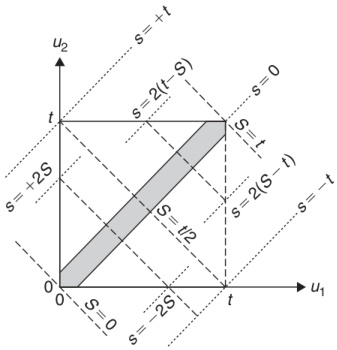
\includegraphics[width=0.30\textwidth]{images/chap15_m27cbe596090a0cf8d4130e8b80d6889e.jpg}
\caption{二重积分 \(I\) 的积分上限与下限，以 \(S\) 和 \(s\) 为变量表示。}
\label{fig:15_15.2}
\end{figure}

其中

\begin{equation}\tag{15.3.26}\label{eq:15.3.26}
C = \int _ { - \infty } ^{\infty} K ( s ) d s .
\end{equation}

?\autoref{eq:15.3.25}??\autoref{eq:15.3.16}?????

\begin{equation}\tag{15.3.27}\label{eq:15.3.27}
\langle v ^{2} ( t ) \rangle = v ^{2} ( 0 ) e ^{- 2 t / \tau} + C \frac { \tau } { 2 } ( 1 - e ^{- 2 t / \tau} ) .
\end{equation}

当 \(t \to \infty\) 时，\(\langle v^2(t) \rangle\) 必须趋近于等分分布值 \(3kT/M\)；因此，

\begin{equation}\tag{15.3.28}\label{eq:15.3.28}
C = 6 k T / M \tau
\end{equation}

因此

\begin{equation}\tag{15.3.29}\label{eq:15.3.29}
\langle v ^{2} ( t ) \rangle = v ^{2} ( 0 ) + \left\{ \frac { 3 k T } { M } - v ^{2} ( 0 ) \right\} ( 1 - e ^{- 2 t / \tau} ) .
\end{equation}

我们注意到，如果 \(\nu^{2}(0)\) 本身等于等分分布值 \(3kT/M\)，那么 \(\langle\nu^{2}(t)\rangle\) 将始终保持不变，这表明一旦达到统计平衡，该系统便具有自然地持续存在的倾向。

?\autoref{eq:15.3.29}??\autoref{eq:15.3.6}?????????????????????? \(\langle r^{2}\rangle\) ? \(t\) ????????????

\begin{equation}\tag{15.3.30}\label{eq:15.3.30}
\frac { d ^{2} } { d t ^{2} } \langle r ^{2} \rangle + \frac { 1 } { \tau } \frac { d } { d t } \langle r ^{2} \rangle = 2 v ^{2} ( 0 ) e ^{- 2 t / \tau} + \frac { 6 k T } { M } ( 1 - e ^{- 2 t / \tau} ) ,
\end{equation}

其解为

\begin{equation}\tag{15.3.31}\label{eq:15.3.31}
\langle r ^{2} \rangle = v ^{2} ( 0 ) \tau ^{2} ( 1 - e ^{- t / \tau} ) ^{2} - \frac { 3 k T } { M } \tau ^{2} ( 1 - e ^{- t / \tau} ) ( 3 - e ^{- t / \tau} ) + \frac { 6 k T \tau } { M } t .
\end{equation}

解 (31) 满足初始条件------在 \(t=0\) 时，\(\langle r^{2}\rangle\) 和其一阶导数均变为零；此外，若取 \(v^{2}(0)=3kT/M\)，则该解可归结为先前所求得的解 (7)。再次强调，在 \(t\ll\tau\) 时，运动呈现可逆性，\(\langle r^{2}\rangle\) 约似 \(v^{2}(0)t^{2}\)；而在 \(t\gg\tau\) 时，则呈现不可逆性，\(\langle r^{2}\rangle\) 约似 \((6BkT)t\)。

? 15.3 ?? 15.4 ????????????? \(\langle v^{2}(t)\rangle\) ? \(\langle r^{2}(t)\rangle\) ????????????\autoref{eq:15.3.29}?\autoref{eq:15.3.31}?????????????????????????????

在布朗发现近 200 年、爱因斯坦和斯莫鲁霍夫斯基进行分析并由佩兰开展早期测量已逾 100 年之后，布朗运动依然是当代研究的热点话题。这一研究热潮的再度兴起，源于胶体在各个领域中技术重要性的不断提升，以及数字视频与计算机图像分析技术的蓬勃发展。一个有趣的例子是，韩等人（2006）在薄型显微镜载玻片上对椭球形颗粒的旋转运动和二维平移运动进行了细致的观测与分析。旋转布朗运动最早由爱因斯坦（1906b）进行分析，并由佩兰（1934、1936）首次实现测量。旋转模式和平移模式均遵循朗之万动力学进行扩散，但平移扩散与旋转扩散相互耦合------因为沿较长轴方向的平移扩散常数大于垂直方向的扩散常数。

\(^{11}\)可以验证的是，

\begin{equation}\tag{15.3.32}\label{eq:15.3.32}
\frac { d } { d t } \langle v ^{2} ( t ) \rangle = \frac { 2 } { \tau } \left[ v ^{2} ( \infty ) - \langle v ^{2} ( t ) \rangle \right] = - \frac { 2 } { \tau } \Delta \langle v ^{2} ( t ) \rangle ,
\end{equation}

其中 \(v^{2}(\infty)=3kT/M\)，而 \(\Delta\langle v^{2}(t)\rangle\) 则表示``相关量偏离其平衡值的偏差''。以这种形式的方程，我们得以获得``弛豫现象''的典型实例，其弛豫时间约为 \(\tau/2\)。

\begin{equation}
p _ { \theta } ( \Delta \theta , t ) = \frac { 1 } { \sqrt { 4 \pi D _ { \theta } t } } \exp \left( - \frac { ( \Delta \theta ) ^{2} } { 4 D _ { \theta } t } \right) ,
\end{equation}

\begin{equation}\tag{15.3.33}\label{eq:15.3.33}
p _ { \mathrm { a } } ( \Delta x _ { \mathrm { a } } , t ) = \frac { 1 } { \sqrt { 4 \pi D _ { \mathrm { a } } t } } \exp \left( - \frac { ( \Delta x _ { \mathrm { a } } ) ^{2} } { 4 D _ { \mathrm { a } } t } \right) ,
\end{equation}

\begin{equation}\tag{15.3.34}\label{eq:15.3.34}
p _ { \mathrm { b } } ( \Delta x _ { \mathrm { b } } , t ) = \frac { 1 } { \sqrt { 4 \pi D _ { \mathrm { b } } t } } \exp \left( - \frac { ( \Delta x _ { \mathrm { b } } ) ^{2} } { 4 D _ { \mathrm { b } } t } \right) ,
\end{equation}

其中扩散常数分别为 \(D_{\theta}\)、\(D_{\mathrm{a}}\) 和 \(D_{\mathrm{b}}\)。实验观测表明，在短时间尺度上（\(t\lesssim\tau_{\theta}=1/(2D_{\theta})\)），系统表现出复杂的二维空间扩散，这与朗之万理论的预测相符。而在长时期（\(t\gg\tau_{\theta}\)）的空间扩散则表现为各向同性，其扩散常数为 \(\overline{D}=(D_{\mathrm{a}}+D_{\mathrm{b}})/2\)。

\section{A ?????????}\label{a-ux8c10ux632fux5b50ux7684ux70edux5e03ux6717ux8fd0ux52a8}

与扩散热布朗粒子的分析方法类似，我们同样可以对处于谐振子势场中的粒子进行分析------该势场能够阻止粒子远离原点扩散，从而更全面地探究位置与速度响应函数之间的关系，以及波动功率谱之间的关联；参见卡普勒（1938年）和钱德拉塞卡尔（1943年）的相关研究。对于质量为 \(M\) 的热布朗粒子，在具有弹簧常数 \(M\omega_{0}^{2}\) 的谐振子势场中，其一维运动方程为

\begin{equation}\tag{15.3.35}\label{eq:15.3.35}
\frac { d ^{2} x } { d t ^{2} } + \gamma \frac { d x } { d t } + \omega _ { 0 } ^{2} x = \frac { F ( t ) } { M } ,
\end{equation}

其中 \(\gamma\)（即 \(6\pi\eta a/M\)）是流体中球形粒子的阻尼系数，该流体的粘度为 \(\eta\)。正如在扩散热布朗运动的情形下一样，作用力 \(F(t)\) 可以是随时间变化的外力，用于探索响应函数；也可以是由于与流体中分子碰撞而产生的随时间变化的随机力，用以分析系统的平衡波动。假设系统在遥远的过去处于平衡状态，则在时刻 \(t\) 的位置可由以下公式给出：

\begin{equation}\tag{15.3.36}\label{eq:15.3.36}
x ( t ) = \int _ { - \infty } ^{t} \chi _ { x x } ( t - t ^{\prime} ) F ( t ^{\prime} ) d t ^{\prime} ,
\end{equation}

其中

\begin{equation}\tag{15.3.37}\label{eq:15.3.37}
\chi _ { x x } ( s ) = \frac { 1 } { M \omega _ { 1 } } e ^{- \frac { \gamma s} { 2 } } \sin { ( \omega _ { 1 } s ) }
\end{equation}

是 \(xx\) 响应函数，\(\omega_{1}=\sqrt{\omega_{0}^{2}-\frac{\gamma^{2}}{4}}\)。12 速度响应则由以下公式给出：

\begin{equation}\tag{15.3.38}\label{eq:15.3.38}
\nu ( t ) = \int _ { - \infty } ^{t} \chi \nu x ( t - t ^{\prime} ) F ( t ^{\prime} ) d t ^{\prime} ,
\end{equation}

¹² 这种形式的响应函数假定振子处于欠阻尼状态。符号 \(\chi_{xx}\) 指的是第15.6.A节中所采用的符号，其中位置坐标 \(x\) 的响应依赖于施加的外场 \(F\)，而该外场通过一项项 \(-F(t)x(t)\) 与哈密顿量耦合。

其中

\begin{equation}\tag{15.3.39}\label{eq:15.3.39}
\chi _ { v x } ( s ) = \frac { 1 } { M } e ^{- \frac { \gamma s} { 2 } } \left( \cos ( \omega _ { 1 } s ) - \frac { \gamma } { 2 \omega _ { 1 } } \sin ( \omega _ { 1 } s ) \right) .
\end{equation}

系统的响应可以分解为一系列独立项的和，这些项涉及一个正弦形外加力 \(\hat{F}(\omega)e^{i\omega t}\)。其形式如下：

\begin{equation}\tag{15.3.40}\label{eq:15.3.40}
\hat { \chi } ( \omega ) = \tilde { \chi } _ { x x } ( \omega ) \hat { F } ( \omega ) ,
\end{equation}

其中，频率依赖的响应函数可以分解为实部和虚部 \(\hat{\chi}_{xx}^{\prime}(\omega)\) 和 \(\hat{\chi}_{xx}^{\prime\prime}(\omega)\)：

\begin{equation}\tag{15.3.41}\label{eq:15.3.41}
\tilde { \chi } _ { x x } ( \omega ) = \int _ { 0 } ^{\infty} \chi _ { x x } ( s ) e ^{i \omega s} d s = \hat { \chi } _ { x x } ^{\prime} ( \omega ) + i \hat { \chi } _ { x x } ^{\prime \prime} ( \omega ) ,
\end{equation}

\begin{equation}\tag{15.3.42}\label{eq:15.3.42}
\hat { \chi } _ { x x } ^{\prime} ( \omega ) = \frac { \omega _ { 0 } ^{2} - \omega ^{2} } { M [ ( \omega _ { 0 } ^{2} - \omega ^{2} ) ^{2} + \gamma ^{2} \omega ^{2} ] } ,
\end{equation}

\begin{equation}\tag{15.3.43}\label{eq:15.3.43}
\hat { \chi } _ { x x } ^{\prime \prime} ( \omega ) = \frac { \gamma \omega } { M [ ( \omega _ { 0 } ^{2} - \omega ^{2} ) ^{2} + \gamma ^{2} \omega ^{2} ] } .
\end{equation}

这里的实部描述了色散特性，而虚部则描述了耗散特性，即它决定了由于正弦形外力而产生的能量平均耗散速率。

现在，我们来考虑粒子在平衡状态下的位置与速度的自然涨落，这些涨落是由于与流体中原子的随机碰撞所引起的。我们将沿用先前用于自由粒子布朗运动的相同朗之万框架。随机力的平均值为零，并且假设其在时间上呈δ函数相关性：

\begin{equation}\tag{15.3.44}\label{eq:15.3.44}
\begin{array}{rlr} & { } & { \langle F \rangle = 0 , } \\& { } & { \langle F ( t ) F ( t ^{\prime} ) \rangle = \Gamma \delta ( t - t ^{\prime} ) , } \end{array}
\end{equation}

其中，\(\Gamma = 2\gamma MkT\)。按照这一选择，粒子的长期平均位置和速度均为零，

\begin{equation}\tag{15.3.45}\label{eq:15.3.45}
\langle x ( t ) \rangle = \langle v ( t ) \rangle = 0 ,
\end{equation}

而且，位置与速度平方的平均值均遵循等能分布定理：

\begin{equation}\tag{15.3.46}\label{eq:15.3.46}
\langle x ^{2} ( t ) \rangle = \frac { k T } { M \omega _ { 0 } ^{2} } ,  \langle v ^{2} ( t ) \rangle = \frac { k T } { M } .
\end{equation}

\(xx\)相关函数由以下公式给出：

\begin{equation}\tag{15.3.47}\label{eq:15.3.47}
\begin{array}{rl} & { G _ { x x } ( t - t ^{\prime} ) = \left\langle x ( t ) x ( t ^{\prime} ) \right\rangle } \\& {  = \frac { k T } { M \omega _ { 0 } ^{2} } \exp \left( \frac { - \gamma | t - t ^{\prime} | } { 2 } \right) \left( \cos \left( \omega _ { 1 } | t - t ^{\prime} | \right) + \frac { \gamma } { 2 \omega _ { 1 } } \sin \left( \omega _ { 1 } | t - t ^{\prime} | \right) \right) , } \end{array}
\end{equation}

而\(xx\)功率谱则由以下公式给出：

\begin{equation}\tag{15.3.48}\label{eq:15.3.48}
S _ { x x } ( \omega ) = \int _ { - \infty } ^{\infty} G _ { x x } ( s ) e ^{i \omega s} d s = \frac { 2 \gamma k T } { M } \frac { 1 } { \left( \omega _ { 0 } ^{2} - \omega ^{2} \right) ^{2} + \gamma ^{2} \omega ^{2} } .
\end{equation}

请注意，方程（39c）中响应函数的虚部 \(\hat{\chi}_{xx}''(\omega)\) 与功率谱 \(S_{xx}(\omega)\) 成正比：

\begin{equation}\tag{15.3.49}\label{eq:15.3.49}
\hat { \chi } _ { x x } ^{\prime \prime} ( \omega ) = \frac { \omega } { 2 k T } S _ { x x } ( \omega ) .
\end{equation}

这一结果表明，通过外力将系统从平衡态驱离所导致的耗散，与平衡状态下自然涨落的功率谱成正比。尽管这一结果最初是针对一种非常特定的模型推导出来的，但它却为我们将在第15.6节中推导出的通用波动-耗散定理提供了一个典型范例。

15.4 理论接近平衡：福克-普朗克方程

????????????????????????????????????? \(r(t)\) ??? \(v(t)\) ?????????????????????????????????????????????????????????????????????15.2???????????????????????????\autoref{eq:15.2.20}????????? \(n(r,t)\)????\autoref{eq:15.2.22}????????? \(\langle r^2(t) \rangle\)?

一种更为通用的视角，用来理解``给定布朗粒子分布如何以及以何种速率接近热力学平衡状态''，是通过所谓的``主方程''来实现的。主方程的简化版本被称为福克-普朗克方程。为作说明，我们考察一组粒子沿 \(x\) 轴的位移 \(x(t)\)。在任意时刻 \(t\)，设 \(f(x,t)dx\) 表示集合中任意一个粒子可能在 \(x\) 与 \(x+dx\) 之间发生位移的概率。该函数

\(f(x,t)\) 必须满足归一化条件

\begin{equation}\tag{15.4.1}\label{eq:15.4.1}
\int _ { - \infty } ^{\infty} f ( x , t ) d x = 1 .
\end{equation}

主方程可写成：

\begin{equation}\tag{15.4.2}\label{eq:15.4.2}
\frac { \partial f ( x , t ) } { \partial t } = \int _ { - \infty } ^{\infty} \{ - f ( x , t ) W ( x , x ^{\prime} ) + f ( x ^{\prime} , t ) W ( x ^{\prime} , x ) \} d x ^{\prime} ,
\end{equation}

其中 \(W(x,x')dx'\delta t\) 表示，在短时间间隔 \(\delta t\) 内，一个位移为 \(x\) 的粒子，转变为位移为 \(x'\) 的概率。13

方程（2）中的积分第一部分，对应于所有将粒子从时间 \(t\) 时的位移 \(x\) 转移到其他位移 \(x'\) 的转变过程，因此构成了函数 \(f(x,t)\) 的净损失；同样地，积分第二部分则对应于所有将粒子从时间 \(t\) 时的其他位移 \(x'\) 转移到位移 \(x\) 的转变过程，因而构成了函数 \(f(x,t)\) 的净收益。14

主方程的结构正是建立在极其简单且直白的前提之上的。当然，在特定条件下，该方程，或其任何推广形式（例如包含速度或动量等坐标参数的版本），都可以被简化为简单的形式

\begin{equation}\tag{15.4.3}\label{eq:15.4.3}
\frac { \partial f } { \partial t } = - \frac { f - f _ { 0 } } { \tau } ,
\end{equation}

这一形式已被证明是研究与传输现象相关问题时非常有用的首次近似方法。在此，\(f_0\) 表示平衡分布函数（当 \(f=f_0\) 时，\(\partial f/\partial t=0\)），而 \(\tau\) 则是弛豫时间，它决定了系统中波动的传播速率，从而决定系统最终达到平衡状态的速度。

在基于式（2）研究布朗运动时，我们可以放心地假设：只有在``紧密相邻''的状态 \(x\) 和 \(x'\) 之间发生的跃迁才具有可观的几率；换言之，跃迁概率函数 \(W(x, x')\) 在 \(x' = x\) 这一值附近呈现出尖峰状分布，并在 \(x\) 之外迅速趋近于零。将区间 \((x' - x)\) 记为 \(\xi\)，我们可写作

\begin{equation}\tag{15.4.4}\label{eq:15.4.4}
W ( x , x ^{\prime} ) \rightarrow W ( x ; \xi ) , \ W ( x ^{\prime} , x ) \rightarrow W ( x ^{\prime} ; - \xi )
\end{equation}

¹³ 我们在此暗中假定一种``马尔可夫''情形：跃迁概率函数 \(W(x, x')\) 仅取决于粒子当前的位置 \(x\)（当然也包括其后续位置 \(x'\)），而与粒子的先前历史无关。

¹⁴ 对于费米子而言，必须考虑泡利不相容原理，该原理决定了系统中``单粒子态的占据情况''；例如，在这种情况下，我们不能考虑那样一种跃迁：该跃迁会将一个粒子转移到一个已经处于占据状态的态。为此，我们需要对主方程进行适当的修正。

其中 \(W(x; \xi)\) 和 \(W(x'; -\xi)\) 在 \(\xi=0\) 这一值附近具有尖峰，并在其他地方迅速趋近于零。¹⁵ 这使我们能够将式（2）的右侧在 \(\xi=0\) 附近展开为泰勒级数。仅保留至二阶项，我们得到

\begin{equation}\tag{15.4.5}\label{eq:15.4.5}
\frac { \partial f ( x , t ) } { \partial t } = - \frac { \partial } { \partial x } \{ \mu _ { 1 } ( x ) f ( x , t ) \} + \frac { 1 } { 2 } \frac { \partial ^{2} } { \partial x ^{2} } \{ \mu _ { 2 } ( x ) f ( x , t ) \} ,
\end{equation}

其中

\begin{equation}\tag{15.4.6}\label{eq:15.4.6}
\mu _ { 1 } ( x ) = \int _ { - \infty } ^{\infty} \xi W ( x ; \xi ) d \xi = \frac { \langle \delta x \rangle _ { \delta t } } { \delta t } = \langle v _ { x } \rangle
\end{equation}

以及

\begin{equation}\tag{15.4.7}\label{eq:15.4.7}
\mu _ { 2 } ( x ) = \int _ { - \infty } ^{\infty} \xi ^{2} W ( x ; \xi ) d \xi = \frac { \langle ( \delta x ) ^{2} \rangle _ { \delta t } } { \delta t } .
\end{equation}

式（5）即所谓的福克-普朗克方程，它在布朗运动与涨落领域中占据着经典的地位。

??????????????????????????????????????? \(F_{x} = -\lambda x\) ????????????????? \(B\)????????????\autoref{eq:15.3.4}????? \(\tau\)?? \(MB\)???????????? \(t\) ???????? \(\tau\) ??????????????? \(-\langle v_{x}\rangle/B\) ???????????????

\begin{equation}\tag{15.4.8}\label{eq:15.4.8}
- \frac { \langle v _ { x } \rangle } { B } + F _ { x } = 0
\end{equation}

因此

\begin{equation}\tag{15.4.9}\label{eq:15.4.9}
\langle v _ { x } \rangle \equiv \mu _ { 1 } ( x ) = - \lambda B x .
\end{equation}

??????\autoref{eq:15.3.10}????

\begin{equation}\tag{15.4.10}\label{eq:15.4.10}
\frac { \langle ( \delta x ) ^{2} \rangle } { \delta t } \equiv \mu _ { 2 } ( x ) = 2 B k T ;
\end{equation}

值得注意的是，此处我们忽略了 \(\lambda\) 对这一量的影响。将式（9）和式（10）代入式（5），我们得到

\begin{equation}\tag{15.4.11}\label{eq:15.4.11}
\frac { \partial f } { \partial t } = \lambda B \frac { \partial } { \partial x } ( x f ) + B k T \frac { \partial ^{2} f } { \partial x ^{2} } .
\end{equation}

\(^{15}\)显然，这一假设将我们的分析范围限制在所谓的``布朗运动近似''范畴内------在这种情况下，我们假定所研究的对象与构成环境的分子之间存在着数量级上的巨大差异。显而易见，若试图用这种分析方法来``理解''分子自身的运动行为，那么我们所能期待的，无非是得出一种``粗略、半定量''的结果。

现在，我们将方程（11）应用于一组布朗粒子，这些粒子最初集中于点 \(x = x_0\)。首先，我们注意到，在没有恢复力的情况下（即 \(\lambda = 0\)），方程（11）会简化为一维扩散方程。

\begin{equation}\tag{15.4.12}\label{eq:15.4.12}
\frac { \partial f } { \partial t } = D \frac { \partial ^{2} f } { \partial x ^{2} }  ( D = B k T ) ,
\end{equation}

???????????\autoref{eq:15.2.19}?\autoref{eq:15.3.11}?????????????????????????????????\autoref{eq:15.2.20}?????? \(f(x,t)\) ????

\begin{equation}\tag{15.4.13}\label{eq:15.4.13}
f ( x , t ) = \frac { 1 } { ( 4 \pi D t ) ^{1 / 2} } \exp \left\{ - \frac { ( x - x _ { 0 } ) ^{2} } { 4 D t } \right\} ,
\end{equation}

其中

\begin{equation}\tag{15.4.14}\label{eq:15.4.14}
{ \overline { { x } } } = x _ { 0 }  { \mathrm { a n d } }  { \overline { { x ^{2} } } } = x _ { 0 } ^{2} + 2 D t ;
\end{equation}

最后的结果表明，粒子所行进的平均平方距离会随时间线性增长，且其值并无上限。然而，恢复力却对粒子的扩散趋势起到了制约作用。例如，在存在此类力（\(\lambda \neq 0\)）的情况下，终端分布 \(f_{\infty}\)（此时 \(\partial f/\partial t = 0\)）由下式决定：

\begin{equation}\tag{15.4.15}\label{eq:15.4.15}
\frac { \partial } { \partial x } ( x f _ { \infty } ) + \frac { k T } { \lambda } \frac { \partial ^{2} f _ { \infty } } { \partial x ^{2} } = 0 ,
\end{equation}

该方程给出

\begin{equation}\tag{15.4.16}\label{eq:15.4.16}
f _ { \infty } ( x ) = \left( \frac { \lambda } { 2 \pi k T } \right) ^{1 / 2} \exp \left( - \frac { \lambda x ^{2} } { 2 k T } \right) ,
\end{equation}

其中

\begin{equation}\tag{15.4.17}\label{eq:15.4.17}
{ \overline { { x } } } = 0  { \mathrm { a n d } }  { \overline { { x ^{2} } } } = k T / \lambda .
\end{equation}

最后的结果表明，粒子 \(x\) 的平均平方值最终必须符合能量均分定理，即 \((\frac{1}{2}\lambda x^2)_{\infty} = \frac{1}{2}kT\)。从平衡统计力学的角度来看，如果我们把具有动能 \(p_x^2/2m\) 和势能 \(\frac{1}{2}\lambda x^2\) 的布朗粒子视为与温度为 \(T\) 的热环境松散耦合，则我们可以直接写出：

\begin{equation}\tag{15.4.18}\label{eq:15.4.18}
f _ { e q } ( x , p _ { x } ) d x d p _ { x } \propto e ^{- ( p _ { x} ^{2} / 2 m + \lambda x ^{2} / 2 ) / k T } d x d p _ { x } .
\end{equation}

通过对 \(p_x\) 进行积分，表达式（18）可直接导出分布函数（16）。

\begin{equation}
p ( x , t ) = \left\{ \frac { \lambda } { 2 \pi k T ( 1 - e ^{- 2 \lambda B t} ) } \right\} ^{1 / 2} \exp \left\{ - \frac { \lambda ( x - x _ { 0 } e ^{- \lambda B t} ) ^{2} } { 2 k T ( 1 - e ^{- 2 \lambda B t} ) } \right\} ,
\end{equation}

其中

\begin{equation}\tag{15.4.19}\label{eq:15.4.19}
\overline { { x } } = x _ { 0 } e ^{- \lambda B t}  \mathrm { a n d }  \overline { { x ^{2} } } = x _ { 0 } ^{2} e ^{- 2 \lambda B t} + \frac { k T } { \lambda } ( 1 - e ^{- 2 \lambda B t} ) ;
\end{equation}

在极限情形下，当\(\lambda \to 0\)时，我们可恢复到纯粹的``扩散''状态，正如方程（13）和（14）所描述的那样；而当\(t \gg (\lambda B)^{-1}\)时，我们则会趋近于``终端''状态，如方程（16）和（17）所描述的那样。图15.5展示了在恢复力与分子碰撞的共同作用下，一整组布朗运动粒子如何逐渐接近平衡态；显然，当前过程的弛豫时间约为\((\lambda B)^{-1}\)。

上述理论易于应用于的一种物理系统，便是动圈式检流计的振荡部分。在此系统中，我们使用一根细丝将线圈与反射镜悬挂在空中，使它们能够绕垂直轴旋转。空气分子与悬吊系统之间的随机、无规则的碰撞会产生一系列强度不断变化的转矩；因此，系统的角位置\(\theta\)不断波动，系统呈现出一种非稳态的零值。这显然是布朗运动的又一个典型例子！在这种情况下，粘性力的作用由检流计的空气阻尼机制（或称电磁阻尼）来承担，而恢复转矩\(N_{\theta} = -c\theta\)则源于细丝的扭转特性。在平衡状态下，我们

预计

\begin{equation}\tag{15.4.20}\label{eq:15.4.20}
\overline { { \left( \frac { 1 } { 2 } c \theta ^{2} \right) } } = \frac { 1 } { 2 } k T ,  \mathrm { t h a t ~ i s , }  \overline { { \theta ^{2} } } = \frac { k T } { c } ;
\end{equation}

将此与方程（17）进行比较。卡普勒（1931）对这类系统的均方偏移量\(\theta^{2}\)进行了实验测定，并将他的研究成果用于推导出一个基于方程（21）的经验公式，从而得到了玻尔兹曼常数\(k\)（或者更确切地说，阿伏伽德罗常数\(N_{A}\)）的数值。卡普勒所使用的系统，其转动惯量\(I=4.552\times10^{-4}\,\mathrm{g}\,\mathrm{cm}^{2}\)，振荡周期\(\tau=1379\,\mathrm{s}\)；据此，恢复转矩的常数\(c\)的值可通过公式\(\tau=2\pi(I/c)^{1/2}\)计算得出，因此

\begin{equation}\tag{15.4.21}\label{eq:15.4.21}
c = 4 \pi ^{2} ( I / \tau ^{2} ) = 9 . 44 3 \times 10 ^{- 9} \mathrm { g } \, \mathrm { c m } ^{2} \mathrm { s } ^{- 2} / \mathrm { r a d } .
\end{equation}

在287.1 K的温度下，观测到的\(\overline{\theta^{2}}\)值为\(4.178 \times 10^{-6}\)。将这些数值代入方程（21），卡普勒得出了：\(k = 1.374 \times 10^{-16}\) erg K\(^{-1}\)。由于气体常数\(R\)等于\(8.31 \times 10^{7}\) erg K\(^{-1}\) mol\(^{-1}\)，他由此推导出阿伏伽德罗常数：\(N_{A} = R/k = 6.06 \times 10^{23}\) mol\(^{-1}\)。

人们或许会认为，将镜像系统置于``真空''外壳中，可以大幅降低由空气分子碰撞所引起的波动。然而事实并非如此------即便在最低可能的压强下，系统中仍然存在着数量极其庞大的分子，它们持续``维持''着布朗运动的活跃状态。不过，故事中颇为有趣的一点在于：由于分子轰击而引起的系统均方偏移量，并不会受到分子密度的影响；对于处于平衡状态的系统而言，这一值完全由温度决定。这一情形在图15.6中得到了极为生动的呈现：图中我们分别绘制了镜像系统的两次振荡曲线，上部曲线是在大气压下获得的，而下部曲线则是在10⁻⁴毫米汞柱的压力下采集的。在这两种情况下，均方根偏差几乎完全相同！尽管如此，我们仍能察觉到这两条曲线之间存在``质量''上的差异，这种差异与波动的``频谱''有关，并且其成因如下：当周围气体的密度较高时，分子脉冲会迅速接连不断，导致系统各次偏移的数量众多，但幅度却相对较小；随着气压的降低， successive脉冲之间的时长逐渐延长，使得每次偏移的数量减少，但幅度却有所增加。然而，无论在长时间内观测到的整体偏移量，其数值基本保持不变。

\begin{figure}[htbp]
\centering
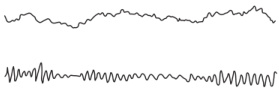
\includegraphics[width=0.25\textwidth]{images/chap15_m157329fad266fd2d2fa6dc87e549cb00.jpg}
\caption{两幅悬挂在空气中的镜像系统热振动曲线；上部曲线为大气压，下部曲线为 \(10^{-4}\) mmHg。}
\label{fig:15_15.6}
\end{figure}

其中

\begin{equation}\tag{15.4.22}\label{eq:15.4.22}
a _ { 0 } = \frac { 1 } { T } \int _ { 0 } ^{T} y ( t ) d t ,
\end{equation}

\begin{equation}\tag{15.4.23}\label{eq:15.4.23}
a _ { n } = \frac { 2 } { T } \int _ { 0 } ^{T} y ( t ) \cos ( 2 \pi n f _ { 0 } t ) d t ,
\end{equation}

以及

\begin{equation}\tag{15.4.24}\label{eq:15.4.24}
b _ { n } = \frac { 2 } { T } \int _ { 0 } ^{T} y ( t ) \sin ( 2 \pi \, n f _ { 0 } t ) d t ;
\end{equation}

在这种情况下，系数 \(a\) 和 \(b\) 将完全确定，并且能够毫无误差地定义变量 \(y(t)\) 的频谱。反之，如果给定的

变量在某种程度上更像是随时间随机变化的函数，那么系数 \(a\) 和 \(b\) 自身就具有统计学性质。要将周期性这一概念应用于此类函数，我们必须将``重复的时间间隔''取为无穷大，即让 \(f_0 \to 0\)。

???????????\autoref{eq:15.4.3}????

\begin{equation}\tag{15.4.25}\label{eq:15.4.25}
a _ { 0 } = \operatorname* { L i m } _ { T \to \infty } { \frac { 1 } { T } } \int _ { 0 } ^{T} y ( t ) d t \equiv \langle y ( t ) \rangle ;
\end{equation}

因此，表示变量 \(y\) 平均值（或直流值）的系数 \(a_{0}\)，既可以通过对该变量进行时间平均（在足够长的时间区间内）来确定，也可以通过在任意时刻 \(t\) 进行集合平均来确定。为了方便起见，且不损失一般性，我们取 \(a_{0}=0\)；换句话说，我们假设已从变量 \(y(t)\) 的实际数值中减去了其平均值 \(\langle y(t)\rangle\)。16

???\autoref{eq:15.4.4}?\autoref{eq:15.4.5}??????????????? \(n\)?

\begin{equation}\tag{15.4.26}\label{eq:15.4.26}
\langle a _ { n } \rangle = \langle b _ { n } \rangle = 0 .
\end{equation}

??????\autoref{eq:15.4.2}??????????????

\begin{equation}\tag{15.4.27}\label{eq:15.4.27}
\begin{array}{rl} & { \langle y ^{2} ( t ) \rangle = \sum _ { n } \frac { 1 } { 2 } \langle a _ { n } ^{2} \rangle + \sum _ { n } \frac { 1 } { 2 } \langle b _ { n } ^{2} \rangle } \\& {  = \sum _ { n } \frac { 1 } { 2 } \Big \{ \langle a _ { n } ^{2} \rangle + \langle b _ { n } ^{2} \rangle \Big \} = \mathrm { c o n s t . } } \end{array}
\end{equation}

? \(\frac{1}{2}\{\langle a_{n}^{2}\rangle+\langle b_{n}^{2}\rangle\}\) ????? \(nf_{0}\) ???????????? \(\langle y^{2}(t)\rangle\) ????????????????????????? \(n\)???? \(\langle a_{n}^{2}\rangle=\langle b_{n}^{2}\rangle\)????\autoref{eq:15.4.8}????

\begin{equation}\tag{15.4.28}\label{eq:15.4.28}
\langle y ^{2} \rangle = \sum _ { n } \langle a _ { n } ^{2} \rangle \simeq \int _ { 0 } ^{\infty} w ( f ) d f ,
\end{equation}

其中

\begin{equation}\tag{15.4.29}\label{eq:15.4.29}
\langle a _ { n } ^{2} \rangle = w ( n f _ { 0 } ) \, \Delta ( n f _ { 0 } ) ,  \mathrm { t h a t ~ i s , }  w ( n f _ { 0 } ) = \frac { 1 } { f _ { 0 } } \, \langle a _ { n } ^{2} \rangle ;
\end{equation}

函数 \(w(f)\) 定义了变量 \(y(t)\) 的功率谱。

现在我们来证明，随机变量 \(y(t)\) 的功率谱 \(w(f)\) 完全由其自相关函数 \(K(s)\) 确定。为此，我们借助于

方程（4），该方程给出了

\begin{equation}\tag{15.4.30}\label{eq:15.4.30}
\langle a _ { n } ^{2} \rangle = 4 f _ { 0 } ^{2} \int _ { 0 } ^{1 / f _ { 0} } \int _ { 0 } ^{1 / f _ { 0} } \langle y ( t _ { 1 } ) y ( t _ { 2 } ) \rangle \cos ( 2 \pi n f _ { 0 } t _ { 1 } ) \cos ( 2 \pi n f _ { 0 } t _ { 2 } ) d t _ { 1 } d t _ { 2 } .
\end{equation}

将变量替换为

\begin{equation}\tag{15.4.31}\label{eq:15.4.31}
S = \frac { 1 } { 2 } ( t _ { 1 } + t _ { 2 } )  \mathrm { a n d }  s = ( t _ { 2 } - t _ { 1 } ) ,
\end{equation}

并牢记，积分所作用的区间 \(T\) 比该随机变量``记忆''持续的时间要长得多，因此我们得到

\begin{equation}\tag{15.4.32}\label{eq:15.4.32}
\langle a _ { n } ^{2} \rangle \simeq 2 f _ { 0 } ^{2} \int _ { S = 0 } ^{1 / f _ { 0} } \int _ { s = - \infty } ^{\infty} K ( s ) \{ \cos ( 2 \pi n f _ { 0 } s ) + \cos ( 4 \pi n f _ { 0 } S ) \} d S d s ;
\end{equation}

将此与从方程（15.3.22）到（15.3.25）及（15.3.26）的推导步骤进行比较。在（12）中，积分中的第二部分在 S 上被积化为零；而第一部分则给出

\begin{equation}\tag{15.4.33}\label{eq:15.4.33}
\langle a _ { n } ^{2} \rangle = 4 f _ { 0 } \int _ { 0 } ^{\infty} K ( s ) \cos ( 2 \pi n f _ { 0 } s ) d s .
\end{equation}

将（13）与（10）进行对比，我们得到了所需的公式

\begin{equation}\tag{15.4.34}\label{eq:15.4.34}
w ( f ) = 4 \int _ { 0 } ^{\infty} K ( s ) \cos ( 2 \pi f s ) d s .
\end{equation}

对 \((14)\) 取逆运算，我们得到

\begin{equation}\tag{15.4.35}\label{eq:15.4.35}
K ( s ) = \int _ { 0 } ^{\infty} w ( f ) \cos ( 2 \pi f s ) d f .
\end{equation}

对于 \(s=0\)，公式（15）给出了一个重要的关系式

\begin{equation}\tag{15.4.36}\label{eq:15.4.36}
K ( 0 ) = \int _ { 0 } ^{\infty} w ( f ) d f = \langle y ^{2} \rangle ;
\end{equation}

同样请参阅方程（9），以及随机变量 \(y\) 自相关函数的定义------即 \(K(s) = \langle y(t_1)y(t_1 + s) \rangle\)。方程（14）和（15），它们连接了互补函数 \(w(f)\) 和 \(K(s)\)，构成了一个由维纳（1930年）和辛钦（1934年）命名的定理。

接下来，我们将探讨随机变量 \(y(t)\) 的一些特殊情况，以说明维纳-辛钦定理的应用。

情形一

如果给定的随机变量 \(y(t)\) 极其不规则、因而难以预测，那么其相关函数 \(K(s)\) 在时间区间 \(s\) 内的延伸范围将微乎其微。\(^{17}\) 我们可以这样写：

\begin{equation}\tag{15.4.37}\label{eq:15.4.37}
K ( s ) = c \delta ( s ) .
\end{equation}

方程（14）随后给出

\begin{equation}\tag{15.4.38}\label{eq:15.4.38}
w ( f ) = 2 c  { \mathrm { f o r ~ a l l ~ } } f .
\end{equation}

一种频谱，其在不同频率上的能量分布均匀，被称为``平坦''或``白色''频谱。然而，我们注意到，如果这种均匀分布在所有频率上------从 0 到 \(\infty\)------都真正成立，那么方程（16）中的积分，其值与 \(\langle y^2 \rangle\) 相同，却会发散！因此，我们预期，在任何现实情境中，相关函数 \(K(s)\) 都不会像（17a）那样尖峰陡峭。通常，\(K(s)\) 会在变量 \(s\) 的一个较小范围内延伸，大约为 \(O(\sigma)\)，而这一范围又会界定一个``频率带''，其频率 \(f = O(1/\sigma)\)，使得函数 \(w(f)\) 随着 \(f\) 跨越这一区域而发生性质变化：在较低频率时，\(w(f) \to \text{常数} \neq 0\)；而在较高频率时，\(w(f) \to \text{常数} = 0\)。图 15.7 展示了这种情形的一种可能表现形式，其中我们相当随意地

\begin{equation}\tag{15.4.39}\label{eq:15.4.39}
K ( s ) = K ( 0 ) \frac { \sin ( a s ) } { a s } \ \ ( a > 0 ) ,
\end{equation}

对于哪一种情况

\begin{equation}\tag{15.4.40}\label{eq:15.4.40}
\begin{array}{r} { w ( f ) = \frac { 2 \pi } { a } K ( 0 )  \mathrm { f o r }  f < \frac { a } { 2 \pi } } \\{ 0   \mathrm { f o r }  f > \frac { a } { 2 \pi } . } \end{array}
\end{equation}

??? \(a \to \infty\) ?????\autoref{eq:15.4.18}????\autoref{eq:15.4.17}??? \(c = \pi a^{-1}K(0)\)?

情形 2

另一方面，如果变量 \(y(t)\) 极其规则，因而具有可预测性，那么其相关函数会在较大的 \(s\) 值范围内延伸；其功率谱则会以``峰值''的形式呈现，这些峰值位于该变量的若干``特征频率''处。在最简单的单色变量情形下，若其特征频率为 \(f^{*}\)，相关函数将为：

\begin{equation}\tag{15.4.41}\label{eq:15.4.41}
K ( s ) = K ( 0 ) \cos ( 2 \pi f ^{*} s ) ,
\end{equation}

¹⁷ 这一结论在很大程度上适用于布朗粒子因不断接收到的分子脉冲而所经历的快速波动力 \(F(t)\)。

\begin{figure}[htbp]
\centering
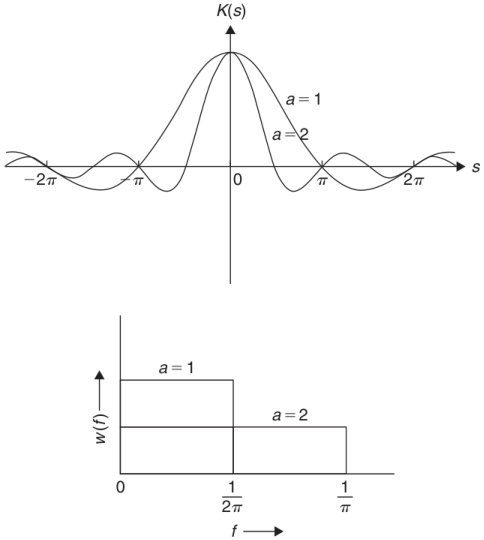
\includegraphics[width=0.43\textwidth]{images/chap15_m4c8e55bacef9097ae461169479aa19e6.jpg}
\caption{给定变量 \(y(t)\) 的自相关函数 \(K(s)\) 与功率分布函数 \(w(f)\)。}
\label{fig:15_15.7}
\end{figure}

这确实满足以下关系

\begin{equation}\tag{15.4.42}\label{eq:15.4.42}
\begin{array}{r} { \int _ { 0 } ^{\infty} w ( f ) d f = \frac { 2 k T } { \pi M } \tan ^{- 1} ( 2 \pi f \tau ) \Big | _ { 0 } ^{\infty} } \\{ = \frac { k T } { M } = \langle v _ { x } ^{2} \rangle , } \end{array}
\end{equation}

与单个速度分量 \(\boldsymbol{\nu}\) 所适用的等能分配定理相一致。对于 \(f \ll \tau^{-1}\)，功率分布几乎与 \(f\) 无关，这意味着功率谱近乎``白噪声''状，且具有

\begin{equation}\tag{15.4.43}\label{eq:15.4.43}
w ( f ) \simeq \frac { 4 k T \tau } { M } = 4 B k T .
\end{equation}

\begin{figure}[htbp]
\centering
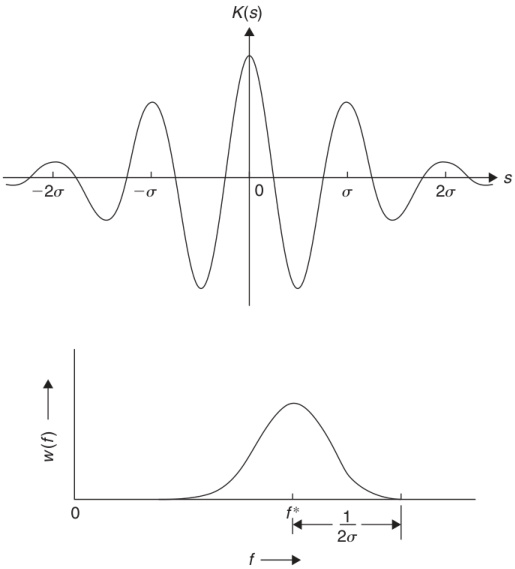
\includegraphics[width=0.46\textwidth]{images/chap15_m218f5b9f42080ef0f3008340a988b90c.jpg}
\caption{窄带滤波变量的自相关函数与功率分布函数示意。}
\label{fig:15_15.9}
\end{figure}
于是我们可以将频率区间 \((f, f+\Delta f)\) 内的速度波动进行如下表示，其中 \(f \ll \tau^{-1}\)，

\begin{equation}\tag{15.4.44}\label{eq:15.4.44}
\langle \Delta v _ { x } ^{2} \rangle _ { ( f , f + \Delta f ) } \simeq w ( f ) \Delta f \simeq ( 4 B k T ) \Delta f .
\end{equation}

一般来说，我们的测量仪器（或者在对粒子进行视觉检查时，用眼睛）都具有有限的响应时间 \(\tau_{0}\)，因此它无法对高于 \(\tau_{0}^{-1}\) 的频率作出响应。此时，观测到的波动可以用``修剪''后的表达式来描述：

\begin{equation}\tag{15.4.45}\label{eq:15.4.45}
\langle v _ { x } ^{2} \rangle _ { \mathrm { o b s } } \simeq \int _ { 0 } ^{1 / \tau _ { 0} } w ( f ) d f = \frac { 2 k T } { \pi M } \tan ^{- 1} \left( 2 \pi \frac { \tau } { \tau _ { 0 } } \right) ,
\end{equation}

而不是使用``完整''的表达式（22）。在典型情况下，布朗粒子的质量 \(M \sim 10^{-12}\) 克，其直径 \(2a \sim 10^{-4}\) 厘米，流体的粘度系数 \(\eta \sim 10^{-2}\) 派斯，因此弛豫时间 \(\tau = M/(6\pi\eta a) \sim 10^{-7}\) 秒。然而，在进行视觉观察时，响应时间 \(\tau_0\) 大约是 \(10^{-1}\) 秒；显然，\(\tau/\tau_0 \sim 10^{-6} \ll 1\)。

方程（25）随后简化为\(^{18}\)

\begin{equation}\tag{15.4.46}\label{eq:15.4.46}
\langle v _ { x } ^{2} \rangle _ { \mathrm { o b s } } \simeq \frac { 4 k T \tau } { M \tau _ { 0 } } \ll \frac { k T } { M } ;
\end{equation}

因此，鉴于响应时间 \(\tau_{0}\) 是有限的，布朗粒子的观测均方根速度将被降低至 \(2(\tau/\tau_{0})^{1/2} \sim 10^{-3}\)；从数值上看，这使得均方根速度从室温下的 \(\sim 10^{-1}\) 厘米/秒降至 \(\sim 10^{-4}\) 厘米/秒。

令人欣慰的是，实际对布朗粒子的观测结果与这一结论完全一致；有关此问题的更详细分析，请参阅麦克唐纳（1950）。上述讨论凸显出这样一个事实：在对波动变量进行观测的过程中，我们的测量仪器只能捕捉到有限范围内的频率信号（由仪器的响应时间决定）；而更高频率的信号则会被直接忽略。

本节的理论可轻松应用于 \((L,R)\) 电路中电子运动的波动。对应于方程（21）至（24），我们现在可以针对电流 \(I\) 的波动得出：

\begin{equation}\tag{15.4.47}\label{eq:15.4.47}
w ( f ) = \frac { 4 k T \tau ^{\prime} } { L } \frac { 1 } { 1 + ( 2 \pi f \tau ^{\prime} ) ^{2} }  \left( \tau ^{\prime} = \frac { L } { R } \right) ,
\end{equation}

由此，

\begin{equation}\tag{15.4.48}\label{eq:15.4.48}
\int _ { 0 } ^{\infty} w ( f ) d f = \frac { k T } { L } = \langle I ^{2} \rangle ,
\end{equation}

与能量均分定理相符：\(\langle\frac{1}{2}LI^{2}\rangle=\frac{1}{2}kT\)。对于 \(f \ll 1/\tau'\)，方程（27）可简化为

\begin{equation}\tag{15.4.49}\label{eq:15.4.49}
w ( f ) \simeq \frac { 4 k T } { R } ,
\end{equation}

这再次表明存在``白噪声''；相应地，对于低频，

\begin{equation}\tag{15.4.50}\label{eq:15.4.50}
\langle \Delta I ^{2} \rangle _ { ( f , f + \Delta f ) } \simeq w ( f ) \Delta f \simeq \frac { 4 k T } { R } \Delta f .
\end{equation}

等价地，我们得到电压波动的表达式为

\begin{equation}\tag{15.4.51}\label{eq:15.4.51}
\langle \Delta V ^{2} \rangle _ { ( f , f + \Delta f ) } \simeq ( 4 R k T ) \Delta f .
\end{equation}

方程（31）构成了所谓的奈奎斯特定理。该定理最早由约翰逊（1927a、b；1928）通过经验发现，后来由奈奎斯特（1927--1928）基于以下原理加以推导：

这一结论涉及热力学第二定律，以及在热平衡状态下，两个电阻之间能量交换的有关论述。\(^{19}\)

\section{波动-耗散定理}\label{ux6ce2ux52a8-ux8017ux6563ux5b9aux7406}

在第15.3节中，我们得到了一项极为重要的结果，即

\begin{equation}\tag{15.4.52}\label{eq:15.4.52}
\begin{array}{rl} & { \frac { 1 } { B } \equiv \frac { M } { \tau } = \frac { M ^{2} } { 6 k T } C = \frac { M ^{2} } { 6 k T } \int _ { - \infty } ^{\infty} K _ { A } ( s ) d s } \\& { = \frac { 1 } { 6 k T } \int _ { - \infty } ^{\infty} K _ { F } ( s ) d s ; } \end{array}
\end{equation}

??\autoref{eq:15.3.4}?\autoref{eq:15.3.26}?\autoref{eq:15.3.28}????\(K_{A}(s)\) ? \(K_{F}(s)\) ???????????????? \(A(t)\) ???? \(F(t)\) ???????

\begin{equation}\tag{15.4.53}\label{eq:15.4.53}
K _ { A } ( s ) = \langle A ( 0 ) \cdot A ( s ) \rangle = \frac { 1 } { M ^{2} } \langle F ( 0 ) \cdot F ( s ) \rangle = \frac { 1 } { M ^{2} } K _ { F } ( s ) .
\end{equation}

???1???????????????????????????????? \(\mathcal{F}(t)\) ??????????? \(1/B\)??????????? \(F(t)\) ??????????????????????\autoref{eq:15.3.2}????????????????????????????????????????????????????1?????????????-?????

该定理最引人注目的特征在于：它以一种根本性的方式，将某一给定系统处于平衡状态时所对应的物理量的波动，与一种耗散过程联系起来------而这种耗散过程在实践中，只有当系统受到外力驱动、使其偏离平衡状态时才会真正发生。由此，我们得以借助对系统在处于某一平衡状态时所发生的热涨落的了解，来确定该系统的非平衡性质。

\(^{19}\)我们注意到，上述结果与爱因斯坦关于导体中电荷波动的原始结果本质上是等价的，即

\begin{equation}\tag{15.4.54}\label{eq:15.4.54}
\langle \delta q ^{2} \rangle _ { t } = \frac { 2 k T } { R } \, t ;
\end{equation}

同样值得注意的是，布朗粒子的结果为：\(\langle x^{2}\rangle_{t}=2BkTt\)。

\(^{20}\)???????? \(K_{A}(s)\) ? \(K_{F}(s)\) ?? \(s=O(\tau^{*})\) ?????\autoref{eq:15.3.21}??????????????????????

\begin{equation}\tag{15.4.55}\label{eq:15.4.55}
K _ { A } ( s ) = \frac { 6 k T } { M ^{2} B } \delta \left( s \right)  \mathrm { a n d }  K _ { F } ( s ) = \frac { 6 k T } { B } \delta ( s ) .
\end{equation}

以这种形式，这些函数仅在 \(s=0\) 时非零。

本章内容！若需了解波动-耗散定理的详细讲解，读者可参考久保（1966）。

??????????????\autoref{eq:15.3.11}??????????? \(D\) ???? \(B\) ??????? \(D = BkT\)??????1?????????

\begin{equation}\tag{15.4.56}\label{eq:15.4.56}
\frac { 1 } { D } = \frac { 1 } { 6 ( k T ) ^{2} } \int _ { - \infty } ^{\infty} K _ { F } ( s ) d s .
\end{equation}

现在，扩散系数 \(D\) 可以直接与随机变量 \(v(t)\) 的自相关函数 \(K_{v}(s)\) 建立联系。为此，我们首先从这样一个事实出发：根据定义，

\begin{equation}\tag{15.4.57}\label{eq:15.4.57}
r ( t ) = \int _ { 0 } ^{t} v ( u ) d u ,
\end{equation}

由此可得

\begin{equation}\tag{15.4.58}\label{eq:15.4.58}
\langle r ^{2} ( t ) \rangle = \int _ { 0 } ^{t} \int _ { 0 } ^{t} \langle v ( u _ { 1 } ) \cdot v ( u _ { 2 } ) \rangle d u _ { 1 } d u _ { 2 } .
\end{equation}

???\autoref{eq:15.3.22}??????????????????

\begin{equation}\tag{15.4.59}\label{eq:15.4.59}
\langle r ^{2} ( t ) \rangle = \int _ { 0 } ^{t / 2} d S \int _ { - 2 S } ^{+ 2 S} K _ { v } ( s ) d s + \int _ { t / 2 } ^{t} d S \int _ { - 2 ( t - S ) } ^{+ 2 ( t - S )} K _ { v } ( s ) d s ;
\end{equation}

?????\autoref{eq:15.3.24}?????

????\autoref{eq:15.3.14}??? \(\nu(t)\)????????? \(\langle\nu^{2}(t)\rangle\) ?????????????? \(\nu(t)\) ?????? \(K_{\nu}(s)\)?? \(\langle\nu^{2}(t)\rangle\) ???????????? \(K_{\nu}(0)\)????????

\begin{equation}\tag{15.4.60}\label{eq:15.4.60}
K _ { \nu } ( s ) = \left\{ \begin{array}{ll} { \nu ^{2} ( 0 ) e ^{- ( 2 t + s ) / \tau} + \frac { 3 k T } { M } e ^{- s / \tau} \left( 1 - e ^{- 2 t / \tau} \right) } & {  \mathrm { f o r }  s > 0 } \\{ \nu ^{2} ( 0 ) e ^{- ( 2 t + s ) / \tau} + \frac { 3 k T } { M } e ^{s / \tau} \left( 1 - e ^{- 2 ( t + s ) / \tau} \right) } & {  \mathrm { f o r }  s < 0 ; } \end{array} \right.
\end{equation}

??????\autoref{eq:15.3.27}??????????????7?????8???????????????

\begin{equation}\tag{15.4.61}\label{eq:15.4.61}
K _ { v } ( s ) = v ^{2} ( 0 ) e ^{- | s | / \tau} + \left\{ \frac { 3 k T } { M } - v ^{2} ( 0 ) \right\} \left( e ^{- | s | / \tau} - e ^{- ( 2 t + s ) / \tau} \right)  \mathrm { f o r ~ a l l ~ } s ;
\end{equation}

?????\autoref{eq:15.3.29}?????????????????

\begin{equation}\tag{15.4.62}\label{eq:15.4.62}
K _ { \nu } ( s ) = \frac { 3 k T } { M } e ^{- | s | / \tau} ,
\end{equation}

这与性质（15.3.20）相一致。需要注意的是，自相关函数 \(K_{\nu}(s)\) 的时间尺度由布朗运动的弛豫时间 \(\tau\) 确定，而 \(\tau\) 的数值要远大于用于确定自相关函数 \(K_{A}(s)\) 和 \(K_{F}(s)\) 时间尺度的特征时间 \(\tau^{*}\)。

?????????????10?????6?????? \(\langle r^{2}\rangle\) ????15.3.7???????????9???????????15.3.31???????15.17????????

\begin{equation}\tag{15.4.63}\label{eq:15.4.63}
\langle r ^{2} \rangle \xrightarrow { t \gg \tau } 6 D t .
\end{equation}

在同样的极限条件下，式（6）会简化为

\begin{equation}\tag{15.4.64}\label{eq:15.4.64}
\langle r ^{2} \rangle \simeq \int _ { 0 } ^{t} d S \int _ { - \infty } ^{\infty} K _ { \nu } ( s ) d s = t \int _ { - \infty } ^{\infty} K _ { \nu } ( s ) d s .
\end{equation}

通过比较这两个结果，我们得到了所需的关联关系：

\begin{equation}\tag{15.4.65}\label{eq:15.4.65}
D = \frac { 1 } { 6 } \int _ { - \infty } ^{\infty} K _ { \nu } ( s ) d s .
\end{equation}

顺便指出，根据式（3）和式（13），我们有

\begin{equation}\tag{15.4.66}\label{eq:15.4.66}
\int _ { - \infty } ^{\infty} K _ { v } ( s ) d s \int _ { - \infty } ^{\infty} K _ { F } ( s ) d s = ( 6 k T ) ^{2} ;
\end{equation}

另请参见问题15.7。

对于那些涉及耗散机制的情形，用来描述涨落-耗散定理的方程得以灵活适应，这并不令人意外。例如，电子在电阻中的运动所引起的涨落，会催生出一种``自发''的热电动势，可记作 \(\mathcal{B}(t)\)。秉承朗之万理论的精神，这种电动势可以被分解为两部分：(i) 一个``平均化''后的部分，即 \(-RI(t)\)，它代表了该情形中的电阻（或耗散）成分；(ii) 一个``快速波动''的部分，即 \(V(t)\)，在较长的时间尺度上，其平均值会趋近于零。于是，电阻中的``自发''电流可由下式给出：

\begin{equation}\tag{15.4.67}\label{eq:15.4.67}
L \frac { d I } { d t } = - R I + V ( t ) ;  \langle V ( t ) \rangle = 0 .
\end{equation}

????????\autoref{eq:15.3.2}????????????????????? \(R\) ??? \(\mathbf{V}(t)\) ????????????????????1????13??????????

\begin{equation}\tag{15.4.68}\label{eq:15.4.68}
R = \frac { 1 } { 6 k T } \int _ { - \infty } ^{\infty} \langle V ( 0 ) \cdot V ( s ) \rangle d s
\end{equation}

或者，等价地，

\begin{equation}\tag{15.4.69}\label{eq:15.4.69}
\frac { 1 } { R } = \frac { 1 } { 6 k T } \int _ { - \infty } ^{\infty} \langle I ( 0 ) \cdot I ( s ) \rangle d s .
\end{equation}

Kubo 在 1957 年和 1959 年对上述结果进行了推广；例如，参见 Kubo（1965）中的问题 6.19，或 Wannier（1966）第 23.2 节。关于推广，电流密度 \(j(t)\) 可用如下表达式表示：

\begin{equation}\tag{15.4.70}\label{eq:15.4.70}
j _ { i } ( t ) = \sum _ { l } \int _ { - \infty } ^{t} E _ { l } ( t ^{\prime} ) \Phi _ { l i } ( t - t ^{\prime} ) d t ^{\prime}  ( i , l = x , y , z ) ;
\end{equation}

在此，\(E(t)\) 表示施加的电场，而

\begin{equation}\tag{15.4.71}\label{eq:15.4.71}
\Phi _ { l i } ( s ) = \frac { 1 } { k T } \langle j _ { l } ( 0 ) j _ { i } ( s ) \rangle .
\end{equation}

显然，量 \(kT\Phi_{li}(s)\) 是涨落向量 \(\mathbf{j}(t)\) 自相关张量的各分量。特别是，若我们考虑静态情形 \(E=(E,0,0)\)，则可得系统的电导率为

\begin{equation}\tag{15.4.72}\label{eq:15.4.72}
\begin{array}{r} { \sigma _ { x x } \equiv \frac { j _ { x } } { E } = \int _ { - \infty } ^{t} \Phi _ { x x } ( t - t ^{\prime} ) d t ^{\prime} = \int _ { 0 } ^{\infty} \Phi _ { x x } ( s ) d s } \\{ = \frac { 1 } { 2 k T } \int _ { - \infty } ^{\infty} \langle j _ { x } ( 0 ) j _ { x } ( s ) \rangle d s , } \end{array}
\end{equation}

这一结果可与式（17）相比较。另一方面，若我们取 \(E=(E\cos\omega t,0,0)\)，则得到

\begin{equation}\tag{15.4.73}\label{eq:15.4.73}
\sigma _ { x x } ( \omega ) = \frac { 1 } { 2 k T } \int _ { - \infty } ^{\infty} \langle j _ { x } ( 0 ) j _ { x } ( s ) \rangle e ^{- i \omega s} d s .
\end{equation}

对式（21）取逆矩阵，可得

\begin{equation}\tag{15.4.74}\label{eq:15.4.74}
\langle j _ { x } ( 0 ) j _ { x } ( s ) \rangle = \frac { k T } { \pi } \int _ { - \infty } ^{\infty} \sigma _ { x x } ( \omega ) e ^{i \omega s} d \omega .
\end{equation}

若我们现在假设 \(\sigma_{xx}(\omega)\) 不依赖于 \(\omega\)（因此，可简称为 \(\sigma\)），则

\begin{equation}\tag{15.4.75}\label{eq:15.4.75}
\langle j _ { x } ( 0 ) j _ { x } ( s ) \rangle = ( 2 k T \sigma ) \delta ( s ) ;
\end{equation}

???? 20?????15.5.17???????????????????????????????????

15.6.A ???????????-????

在本节中，我们将证明：热力学系统对微小驱动力的非平衡响应，与平衡涨落的时间依赖性有着极为普遍的关联。事后看来，这其实并不令人意外------因为自然产生的、围绕平衡态的涨落，同样会引发可观测量偏离其平均值的微小变化。系统对这些自然涨落的响应，应当与系统对由微小驱动力引起的偏离平衡态的响应相同；参见Martin（1968）、Forster（1975）以及Mazenko（2006）的相关研究。

我们来计算由一个随时间线性耦合于某可观测量B的微小时间依赖性外加场h(t)所引起的可观测量A的时间依赖性变化。此时，系统的哈密顿量变为

\begin{equation}\tag{15.6.1}\label{eq:15.6.1}
H ( t ) = H _ { 0 } - h ( t ) B ,
\end{equation}

其中H₀为平衡态下的未扰动哈密顿量。令人惊叹的是，要计算系统对驱动场的非平衡响应，最简便的方法是采用第5.1节中发展起来的量子力学密度矩阵方法。平衡态密度矩阵可表示为

\begin{equation}\tag{15.6.2}\label{eq:15.6.2}
\hat { \rho } _ { \mathrm { e q } } = \frac { \exp ( - \beta H _ { 0 } ) } { \mathrm { T r } \left( \exp ( - \beta H _ { 0 } ) \right) } ,
\end{equation}

其中，平衡态平均值涉及对密度矩阵进行求和：

\begin{equation}\tag{15.6.3}\label{eq:15.6.3}
\langle A \rangle _ { \mathrm { e q } } = \mathrm { T r } \left( A \hat { \rho } _ { \mathrm { e q } } \right) .
\end{equation}

当哈密顿量中包含一个微小的时间依赖性场h(t)时，这一附加项会略微使系统偏离平衡态。我们假设该场在遥远的过去为零，因此系统最初处于由

哈密顿量H₀。随后我们开启该场，并测量可观测量A与其平衡值之间的时间依赖性偏差。微小的时间依赖性外加场h(t)会对密度矩阵产生微小的变化

\begin{equation}\tag{15.6.4}\label{eq:15.6.4}
\hat { \rho } ( t ) = \hat { \rho } _ { \mathrm { e q } } + \delta \hat { \rho } ( t ) .
\end{equation}

方程（5.1.10）中密度矩阵的运动方程给出

\begin{equation}\tag{15.6.5}\label{eq:15.6.5}
\frac { \partial \hat { \rho } } { \partial t } = \frac { \partial \delta \hat { \rho } } { \partial t } = \frac { 1 } { i \hbar } \left[ H , \hat { \rho } ( t ) \right] \approx \frac { 1 } { i \hbar } \left( \left[ H _ { 0 } , \delta \hat { \rho } \right] - h ( t ) \left[ B , \hat { \rho } _ { \mathrm { e q } } \right] \right) ,
\end{equation}

其中 \([\, , \,]\) 表示对易子。由于我们仅考虑系统对外加场的线性响应，因此忽略与 \(h(t)[B,\delta\hat{\rho}]\) 成比例的高阶项。通过解方程（28）以求得密度矩阵的时间依赖性变化，我们得到

\begin{equation}\tag{15.6.6}\label{eq:15.6.6}
\delta \hat { \rho } ( t ) = \frac { i } { \hbar } \int _ { - \infty } ^{t} h ( t ^{\prime} ) \exp \left( \frac { - i H _ { 0 } ( t - t ^{\prime} ) } { \hbar } \right) \left[ B , \hat { \rho } _ { \mathrm { e q } } \right] \exp \left( \frac { i H _ { 0 } ( t - t ^{\prime} ) } { \hbar } \right) d t ^{\prime} .
\end{equation}

这种形式采用了相互作用表示法，在这种表示法中，算符会因未扰动哈密顿量H₀而随时间演化。我们可以利用密度矩阵在时刻t的变化，来计算可观测量A与其平衡值相比的改变量，即

\begin{equation}\tag{15.6.7}\label{eq:15.6.7}
\langle \delta A ( t ) \rangle = \langle A ( t ) \rangle - \langle A \rangle _ { \mathrm { e q } } = \mathrm { T r } \left( A \hat { \rho } ( t ) \right) - \mathrm { T r } \left( A \hat { \rho } _ { \mathrm { e q } } \right) = \mathrm { T r } \left( A \delta \hat { \rho } ( t ) \right) .
\end{equation}

利用迹的循环性质\(\operatorname{Tr}\left(QRS\right)=\operatorname{Tr}\left(SQR\right)\)，我们发现\(\left\langle\delta A(t)\right\rangle\)是响应函数与外加场卷积的结果：

\begin{equation}\tag{15.6.8}\label{eq:15.6.8}
\langle \delta A ( t ) \rangle = \frac { i } { \hbar } \int _ { - \infty } ^{t} \left\langle \left[ A ( t ) , B ( t ^{\prime} ) \right] \right\rangle _ { \mathrm { e q } } h ( t ^{\prime} ) d t ^{\prime} .
\end{equation}

请注意，系统对驱动力的这一非平衡响应函数，依赖于不同时间点观测量 \(A\) 和 \(B\) 的交换子的平衡平均值。场对观测量 \(A\) 的作用是因果的，因为 \(\langle\delta A(t)\rangle\) 仅取决于较早时刻施加的场。由于该关系呈线性、具有时间平移不变性且为因果关系，因此 \(\langle\delta A\rangle\) 和 \(h\) 的傅里叶谱分别为

\begin{equation}\tag{15.6.9}\label{eq:15.6.9}
\delta \hat { A } ( \omega ) = \int _ { - \infty } ^{\infty} \langle \delta A ( t ) \rangle \, e ^{i \omega t} d t , \, \mathrm { a n d }
\end{equation}

\begin{equation}\tag{15.6.10}\label{eq:15.6.10}
\hat { h } ( \omega ) = \int _ { - \infty } ^{\infty} h ( t ) e ^{i \omega t} d t ,
\end{equation}

由以下关系联系在一起：

\begin{equation}\tag{15.6.11}\label{eq:15.6.11}
\delta \hat { A } ( \omega ) = \left( \hat { \chi } _ { A B } ^{\prime} ( \omega ) + i \hat { \chi } _ { A B } ^{\prime \prime} ( \omega ) \right) \hat { h } ( \omega ) ,
\end{equation}

其中 \(\hat{\chi}_{AB}^{\prime\prime}(\omega)\) 的表达式为

\begin{equation}\tag{15.6.12}\label{eq:15.6.12}
\hat { \chi } _ { A B } ^{\prime \prime} ( \omega ) = \frac { 1 } { 2 \hbar } \int _ { - \infty } ^{\infty} \langle [ A ( t ) , B ( 0 ) ] \rangle _ { \mathrm { e q } } e ^{i \omega t} d t .
\end{equation}

量 \(\hat{\chi}_{AB}^{\prime}(\omega)\) 通过克劳斯---克罗尼格关系给出，该关系利用了 \(\hat{\chi}_{AB}^{\prime\prime}(\omega)\) 在无穷积分中的主部分 \(P\)：

\begin{equation}\tag{15.6.13}\label{eq:15.6.13}
\hat { \chi } _ { A B } ^{'} ( \omega ) = P \int _ { - \infty } ^{\infty} \frac { \hat { \chi } _ { A B } ^{' \prime} ( \omega ^{\prime} ) } { \omega ^{\prime} - \omega } \frac { d \omega ^{\prime} } { \pi } .
\end{equation}

若 \(A\) 和 \(B\) 是同一算子，则 \(\hat{\chi}_{AA}^{\prime}(\omega)\) 和 \(\hat{\chi}_{AA}^{\prime\prime}(\omega)\) 分别为响应函数的实部和虚部。若 \(A\) 和 \(B\) 在时间反演下具有相同的对称性，则 \(\omega\hat{\chi}_{AB}^{\prime\prime}(\omega)\) 为实数，并且是 \(\omega\) 的偶函数。对于一组观测量 \(A_{i}\)，响应函数组 \(\omega\hat{\chi}_{ij}^{\prime\prime}(\omega)\) 构成一个对称的正定矩阵，可用来衡量外部驱动力所导致的能量耗散速率。有关一般性因果关系的讨论，请参阅 Jackson（1999），而关于此计算的详细内容，则可参考 Martin（1968）、Forster（1975）或 Mazenko（2006）。

接下来，我们来探讨观测量 \(A\) 和 \(B\) 波动之间的平衡时间相关性，即

\begin{equation}\tag{15.6.14}\label{eq:15.6.14}
G _ { A B } ( t - t ^{\prime} ) = \left\langle \delta A ( t ) \delta B ( t ^{\prime} ) \right\rangle _ { \mathrm { e q } } .
\end{equation}

在相同的时间点，这一指标测量的是第 15.1 节中所描述的 \(AB\) 平衡波动，亦即 \(G_{AB}(0)=\langle\delta A\delta B\rangle_{\mathrm{eq}}\)。\(AB\) 平衡波动的功率谱由如下定义：

\begin{equation}\tag{15.6.15}\label{eq:15.6.15}
S _ { A B } ( \omega ) = \int _ { - \infty } ^{\infty} G _ { A B } ( t ) e ^{i \omega t} d t = \int _ { - \infty } ^{\infty} \langle \delta A ( t ) \delta B ( 0 ) \rangle _ { \mathrm { e q } } e ^{i \omega t} d t .
\end{equation}

\autoref{eq:15.6.34}?\autoref{eq:15.6.37}? \(S_{AB}(\omega)\) ? \(\hat{\chi}_{AB}^{\prime\prime}(\omega)\) ??????????????????????????????????-?????

\begin{equation}\tag{15.6.16}\label{eq:15.6.16}
\hat { \chi } _ { A B } ^{\prime \prime} ( \omega ) = \frac { 1 } { 2 \hbar } \left( 1 - e ^{- \beta \hbar \omega} \right) S _ { A B } ( \omega ) .
\end{equation}

功率谱 \(S_{AB}(\omega)\) 测量的是平衡波动，而 \(\hat{\chi}_{AB}''(\omega)\) 则与因随时间变化的外加场而产生的平均功率耗散速率成正比。当 \(\hbar\omega/kT\to0\) 时，即可得到涨落-耗散定理的经典极限，其结果为

\begin{equation}\tag{15.6.17}\label{eq:15.6.17}
\hat { \chi } _ { A B } ^{\prime \prime} ( \omega ) = \frac { \omega } { 2 k T } S _ { A B } ( \omega ) ;
\end{equation}

???\autoref{eq:15.3.45}?????????-??????????????? Martin?1968??Forster?1975??? Mazenko?2006??

\section{B ?????}\label{b-ux975eux5f39ux6027ux6563ux5c04}

非弹性散射是测量材料动力学行为的重要实验技术。通过测量从样品中散射出的辐射强度随波矢转移量以及相对于入射单色辐射源的频率变化而变化的情况，可以对材料中的时空相关性进行测量。目前，该技术已广泛应用于中子、电子、光和X射线的散射。散射波中的频率变化是由样品中量子激发引起的非弹性散射所致；参见Forster（1975）、Squires（1997）以及Mazenko（2006）。

频率依赖的散射强度与动力学结构因子成正比。

\begin{equation}\tag{15.6.18}\label{eq:15.6.18}
S ( \pmb { k } , \omega ) = \frac { 1 } { N } \int _ { - \infty } ^{\infty} \left\langle \sum _ { i , j } e ^{- i \pmb { k} \cdot ( \pmb { r } _ { i } ( t ) - \pmb { r } _ { j } ( 0 ) ) } \right\rangle e ^{i \omega t} d t ,
\end{equation}

其中，\(k\) 表示散射过程的波矢转移量，\(\omega\) 表示与入射束相比的频率差。\(\omega\) 的正值对应于检测到的频率低于入射束的频率。动力学结构因子 \(S(k,\omega)\) 同时编码了材料中波动的空间与时间平衡相关性，并且可以分解为两部分：一部分表示来自不同时间的单个粒子的散射，另一部分则表示来自不同粒子的散射：

\begin{equation}\tag{15.6.19}\label{eq:15.6.19}
S ( \pmb { k } , \omega ) = S _ { \mathrm { s e l f } } ( \pmb { k } , \omega ) + S _ { \mathrm { c o h e r e n t } } ( \pmb { k } , \omega ) ,
\end{equation}

\begin{equation}\tag{15.6.20}\label{eq:15.6.20}
S _ { \mathrm { s e l f } } ( \pmb { k } , \omega ) = \frac { 1 } { N } \int _ { - \infty } ^{\infty} \left\langle \sum _ { i } e ^{- i \pmb { k} \cdot ( \pmb { r } _ { i } ( t ) - \pmb { r } _ { i } ( 0 ) ) } \right\rangle e ^{i \omega t} d t ,
\end{equation}

\begin{equation}\tag{15.6.21}\label{eq:15.6.21}
S _ { \mathrm { c o h e r e n t } } ( \pmb { k } , \omega ) = \frac { 1 } { N } \int _ { - \infty } ^{\infty} \left\langle \sum _ { i \neq j } e ^{- i \pmb { k} \cdot ( \pmb { r } _ { i } ( t ) - \pmb { r } _ { j } ( 0 ) ) } \right\rangle e ^{i \omega t} d t .
\end{equation}

动力学结构因子 \(S(\boldsymbol{k},\omega)\) 也可以用时间依赖密度 \(n(\boldsymbol{r},t)\) 的时空傅里叶变换来表示，从而将其与第15.6.A节所定义的功率谱联系起来：

\begin{equation}\tag{15.6.22}\label{eq:15.6.22}
S ( \pmb { k } , \omega ) = S _ { A B } ( \omega ) = \int _ { - \infty } ^{\infty} \langle \delta A ( t ) \delta B ( 0 ) \rangle \, e ^{i \omega t} \, d t ,
\end{equation}

\begin{equation}\tag{15.6.23}\label{eq:15.6.23}
\delta A ( t ) = \frac { 1 } { \sqrt { N } } \int e ^{- i \mathbf { k} \cdot \mathbf { r } } \delta n ( \mathbf { r } , t ) d \mathbf { r } = \frac { 1 } { \sqrt { N } } \hat { n } _ { - \mathbf { k } } ( t ) ,
\end{equation}

\begin{equation}\tag{15.6.24}\label{eq:15.6.24}
\delta B ( 0 ) = \frac { 1 } { \sqrt { N } } \int e ^{i \mathbf { k} \cdot \mathbf { r } } \delta n ( \mathbf { r } , 0 ) d \mathbf { r } = \frac { 1 } { \sqrt { N } } \hat { n } _ { \mathbf { k } } ( 0 ) .
\end{equation}

正频率变化 \(\omega > 0\) 表示在材料中产生能量为 \(\hbar\omega\) 的量子激发的散射事件，这些事件被称为斯托克斯散射。负频率变化则被称为反斯托克斯散射，对应于以能量为 \(\hbar\omega\) 的方式破坏材料中某项激发的散射事件。由于激发必须先存在，才能被摧毁，因此在平衡状态下，反斯托克斯散射的速率相较于斯托克斯散射的速率，会因激发的玻尔兹曼因子而降低：

\begin{equation}\tag{15.6.25}\label{eq:15.6.25}
S ( \pmb { k } , - \omega ) = e ^{- \beta \hbar \omega} S ( \pmb { k } , \omega ) .
\end{equation}

在拉曼散射中，这种关系有时被用来测量样品的温度。当激发能量与热能相比较小时，即 \(\hbar\omega \ll kT\) 时，斯托克斯峰和反斯托克斯峰的高度是关于称的。式（10.7.18） 中的静态结构因子 \(S(\boldsymbol{k})\) 是通过对 \(S(\boldsymbol{k},\omega)\) 在所有 \(\omega\) 上进行积分得到的：

\begin{equation}\tag{15.6.26}\label{eq:15.6.26}
S ( k ) = \frac { 1 } { 2 \pi } \int _ { - \infty } ^{\infty} S ( k , \omega ) d \omega .
\end{equation}

这一方法能够区分等时散射事件，并对应于那些无法分辨材料中激发所引起的能量变化的准弹性散射测量。

通常测量的三种非弹性激光散射类型包括：拉曼散射、布里渊散射和瑞利散射。拉曼散射用于测量原子和分子的电子、振动和转动激发、电子能带结构以及光学声子模式；布里渊散射则用于测量长波长的声学声波模式。拉曼散射和布里渊散射峰的宽度由各自模式的寿命决定。瑞利散射则测量以 \(\omega=0\) 为中心、宽度与热扩散率成正比的热扩散模式。可见光的波长相较于原子尺度而言较大，因此，光散射过程中可能实现的波矢传递量，与布里渊区的尺寸相比微乎其微。然而，在非弹性X射线散射和中子散射中，这一限制得以消除------实验可以探测远离布里渊区中心的波矢。

激光束从液体中发生的动力学散射包含三个峰值：一个以 \(\omega=0\) 为中心的瑞利峰，源于液体中热涨落的散射；以及两个斯托克斯峰和反斯托克斯峰，它们分别位于 \(\omega_{k}\approx\pm ck\)，源自声子的散射，而声速为 \(c\)。对于该波矢和频率范围内的散射，由于 \(\hbar\omega \ll kT\)，动力学结构因子在 \(\omega\) 上是对称的。图 15.10 展示了早期对液体动力学结构因子的布里渊散射测量结果。

涨落-耗散定理使得我们能够基于系统在远离平衡状态时的流体力学响应，发展出关于动力学结构因子的理论。在流体的情况下，压力和温度的微小扰动会引发声波的传播以及热扩散。由此产生以下结果：

\begin{figure}[htbp]
\centering
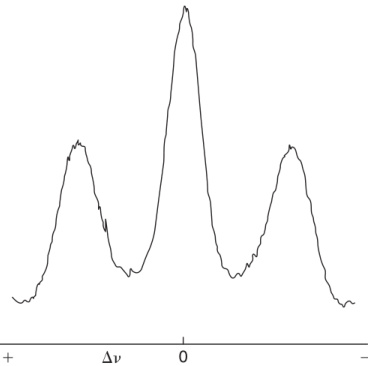
\includegraphics[width=0.33\textwidth]{images/chap15_m5c2a1bb2c993c9955e7917bd0a33b25f.jpg}
\caption{四氯化碳动力学结构因子的布里渊散射结果。}
\label{fig:15_15.10}
\end{figure}
动力学结构因子的理论表达式：
\begin{equation*}
S ( k , \omega ) = S ( k ) \left[ \left( \frac { \gamma - 1 } { \gamma } \right) \frac { 2 D _ { T } k ^{2} } { \omega ^{2} + ( D _ { T } k ^{2} ) ^{2} } + \frac { 1 } { \gamma } \left( \frac { \Gamma k ^{2} } { ( \omega ^{2} - c ^{2} k ^{2} ) ^{2} + ( \Gamma k ^{2} ) ^{2} } + \frac { \Gamma k ^{2} } { ( \omega ^{2} + c ^{2} k ^{2} ) ^{2} + ( \Gamma k ^{2} ) ^{2} } \right) \right] .
\end{equation*}

式（45）中的参数包括热扩散率\(D_{T}\)、声速\(c\)以及声衰减系数\(\Gamma\)，而\(\gamma = C_{P}/C_{V}\)则是恒压热容与恒容热容之比；参见Forster（1975）及Hansen和McDonald（1986）的相关论述。

第15.7节　翁萨格关系

大多数物理现象都表现出某种对称性，有时被称为``互易性''，这种对称性源于微观过程在宏观现象背后所具有的某些基本特性。一个显著的例子出现在不可逆过程的热力学中------在处理各种流动过程时，例如热流、电流、物质传递等。这些流动（或``电流''）是由``力''驱动的，比如温度差、电势差、压力差等，而这些力之所以发挥作用，是因为一种自然倾向。

在那些处于非平衡状态、却能逐渐接近平衡状态的物理系统中。如果系统的当前状态离平衡态并不相差太远，那么我们就可以假设力\(X_i\)与电流\(x_i\)之间存在线性关系：

\begin{equation}\tag{15.6.27}\label{eq:15.6.27}
\dot { x } _ { i } = \gamma _ { i j } X _ { j } ,
\end{equation}

其中\(\gamma_{ij}\)为系统的动力学系数。²¹ 这些系数的简单例子包括热导率、电导率、扩散系数等。然而，系统中也存在非对角元素\(\gamma_{ij}(i \neq j)\)，它们可能为零，也可能不为零；正是这些元素导致了所谓的``交叉效应''。本节所研究的内容，正是基于矩阵\(\gamma_{ij}\)的对称性特征。

解决这一问题最直观的方法，是将系统在扰动状态下的熵 \(S(x_i)\) 与其在相应平衡状态下的最大值 \(S(\tilde{x}_i)\) 进行比较。正是函数 \(S(x_i)\) 自然趋于其最大值 \(S(\tilde{x}_i)\) 的趋势，促使驱动力 \(X_i\) 被激活；这些力催生出电流 \(\tilde{x}_i\)，而这些电流则以``坐标'' \(x_i\) 为向量，将其引导至平衡态的值 \(\tilde{x}_i\)。若偏差 \((x_i - \tilde{x}_i)\) 很小，则可将函数 \(S(x_i)\) 表示为围绕 \(x_i = \tilde{x}_i\) 值展开的泰勒级数；仅保留至二阶项，我们得到：

\begin{equation}\tag{15.6.28}\label{eq:15.6.28}
\begin{array}{rl} { S ( x _ { i } ) = S ( \tilde { x } _ { i } ) + \left( \frac { \partial S } { \partial x _ { i } } \right) _ { x _ { i } = \tilde { x } _ { i } } ( x _ { i } - \tilde { x } _ { i } ) } & { } \\{ + \frac { 1 } { 2 } \left( \frac { \partial ^{2} S } { \partial x _ { i } \partial x _ { j } } \right) _ { x _ { i , j } = \tilde { x } _ { i , j } } ( x _ { i } - \tilde { x } _ { i } ) ( x _ { j } - \tilde { x } _ { j } ) . } & { } \end{array}
\end{equation}

鉴于函数 \(S(x_i)\) 在 \(x_i = \tilde{x}_i\) 处取得最大值，其一阶导数为零；因此，我们可以写出

\begin{equation}\tag{15.6.29}\label{eq:15.6.29}
\Delta S \equiv S ( x _ { i } ) - S ( \tilde { x } _ { i } ) = - \frac { 1 } { 2 } \beta _ { i j } ( x _ { i } - \tilde { x } _ { i } ) ( x _ { j } - \tilde { x } _ { j } ) ,
\end{equation}

其中

\begin{equation}\tag{15.6.30}\label{eq:15.6.30}
\beta _ { i j } = - \left( \frac { \partial ^{2} S } { \partial x _ { i } \partial x _ { j } } \right) _ { x _ { i , j } = \tilde { x } _ { i , j } } = \beta _ { j i } .
\end{equation}

驱动力 \(X_{i}\) 可以按照热力学第二定律的精神来定义，即

\begin{equation}\tag{15.6.31}\label{eq:15.6.31}
X _ { i } = \left( \frac { \partial S } { \partial x _ { i } } \right) = - \beta _ { i j } ( x _ { j } - \tilde { x } _ { j } ) .
\end{equation}

在撰写式（1）及其他后续方程时，我们遵循求和约定------该约定自动对重复的索引进行求和。

??????????????? \(X_i\) ??? \((x_i - \tilde{x}_i)\) ?????????????????????????\autoref{eq:15.1.2}?\(x_iX_j\) ????????????

\begin{equation}\tag{15.6.32}\label{eq:15.6.32}
\langle x _ { i } X _ { j } \rangle = \frac { \int _ { - \infty } ^{\infty} ( x _ { i } X _ { j } ) \exp \left\{ - \frac { 1 } { 2 k } \beta _ { i j } ( x _ { i } - \tilde { x } _ { i } ) ( x _ { j } - \tilde { x } _ { j } ) \right\} \prod _ { i } d x _ { i } } { \int _ { - \infty } ^{\infty} \exp \left\{ - \frac { 1 } { 2 k } \beta _ { i j } ( x _ { i } - \tilde { x } _ { j } ) ( x _ { j } - \tilde { x } _ { j } ) \right\} \prod _ { i } d x _ { i } } ;
\end{equation}

由于此处的积分不会因变量的较大取值而产生显著贡献，因此积分限已扩展至 \(-\infty\) 和 \(+\infty\)。同样地，

\begin{equation}\tag{15.6.33}\label{eq:15.6.33}
\langle x _ { i } \rangle = \frac { \int _ { - \infty } ^{\infty} x _ { i } \exp \left\{ - \frac { 1 } { 2 k } \beta _ { i j } ( x _ { i } - \tilde { x } _ { i } ) ( x _ { j } - \tilde { x } _ { j } ) \right\} \prod _ { i } d x _ { i } } { \int _ { - \infty } ^{\infty} \exp \left\{ - \frac { 1 } { 2 k } \beta _ { i j } ( x _ { i } - \tilde { x } _ { i } ) ( x _ { j } - \tilde { x } _ { j } ) \right\} \prod _ { i } d x _ { i } } = \tilde { x } _ { i } .
\end{equation}

对式（7）关于 \(\tilde{x}_{j}\) 求导，并牢记分母中的积分是一个常数、与各量 \(\tilde{x}_{i}\) 的实际值无关，再将所得表达式与式（6）进行比较，我们得到了一个极为重要的结论

\begin{equation}\tag{15.6.34}\label{eq:15.6.34}
\langle x _ { i } X _ { j } \rangle = - k \delta _ { i j } .
\end{equation}

接下来，我们转向论证的关键点。首先，我们注意到，尽管式（1）所讨论的是不可逆现象，但这些现象背后的微观过程却遵循时间反演法则，这意味着相关变量的时间相关性在向前或向后测量时均保持一致。因此，

\begin{equation}\tag{15.6.35}\label{eq:15.6.35}
\langle x _ { i } ( 0 ) x _ { j } ( s ) \rangle = \langle x _ { i } ( 0 ) x _ { j } ( - s ) \rangle ;
\end{equation}

此外，通过将时间的原点进行平移，

\begin{equation}\tag{15.6.36}\label{eq:15.6.36}
\langle x _ { i } ( 0 ) x _ { j } ( - s ) \rangle = \langle x _ { i } ( s ) x _ { j } ( 0 ) \rangle .
\end{equation}

将式（9）与式（10）相结合，我们得到

\begin{equation}\tag{15.6.37}\label{eq:15.6.37}
\langle x _ { i } ( 0 ) x _ { j } ( s ) \rangle = \langle x _ { i } ( s ) x _ { j } ( 0 ) \rangle .
\end{equation}

若我们从该等式的两边分别减去量 \(\langle x_{i}(0)x_{j}(0)\rangle\)，再将所得等式除以 \(s\)，并令 \(s \to 0\)，则可得

\begin{equation}\tag{15.6.38}\label{eq:15.6.38}
\langle x _ { i } ( 0 ) \dot { x } _ { j } ( 0 ) \rangle = \langle \dot { x } _ { i } ( 0 ) x _ { j } ( 0 ) \rangle .
\end{equation}

将（1）中的表达式代入，并利用（8），我们可在（12）的左侧得到

\begin{equation}\tag{15.6.39}\label{eq:15.6.39}
\langle x _ { i } ( 0 ) \gamma _ { j l } X _ { l } ( 0 ) \rangle = - k \gamma _ { j l } \delta _ { i l } = - k \gamma _ { j i }
\end{equation}

而在其右侧

\begin{equation}\tag{15.6.40}\label{eq:15.6.40}
\langle \gamma _ { i l } X _ { l } ( 0 ) x _ { j } ( 0 ) \rangle = - k \gamma _ { i l } \delta _ { j l } = - k \gamma _ { i j } .
\end{equation}

由此可知，

\begin{equation}\tag{15.6.41}\label{eq:15.6.41}
\gamma _ { i j } = \gamma _ { j i } .
\end{equation}

方程（13）构成了翁萨格互易关系；这些关系最早由翁萨格于1931年推导出来，并已成为不可逆现象热力学中不可或缺的一部分。

鉴于方程（1）和方程（13），电流 \(\dot{x}_{i}\) 可写为

\begin{equation}\tag{15.6.42}\label{eq:15.6.42}
\dot { x } _ { i } = \frac { \partial f } { \partial X _ { i } } ,
\end{equation}

其中，生成函数 \(f\) 是力 \(X_i\) 的二次函数：

\begin{equation}\tag{15.6.43}\label{eq:15.6.43}
f = \frac { 1 } { 2 } \gamma _ { i j } X _ { i } X _ { j } .
\end{equation}

函数 \(f\) 至关重要，因为它直接决定了系统熵随时间变化的速率：

\begin{equation}\tag{15.6.44}\label{eq:15.6.44}
\dot { S } = \frac { \partial S } { \partial x _ { i } } \dot { x } _ { i } = X _ { i } \dot { x } _ { i } = X _ { i } \frac { \partial f } { \partial X _ { i } } = 2 f .
\end{equation}

当系统接近平衡态时，其熵必将向平衡值 \(S(\tilde{x}_i)\) 增加。因此，函数 \(f\) 必须为正定函数，这为系数 \(\gamma_{ij}\) 带来了若干限制条件。

与方程（1）类似，我们同样可以写出

\begin{equation}\tag{15.6.45}\label{eq:15.6.45}
\dot { X } _ { i } = \zeta _ { i j } ( x _ { j } - \tilde { x } _ { j } ) ,
\end{equation}

量 \(\zeta_{ij}\) 则是与系统相关的另一组系数。另一方面，根据方程（1）和方程（5），我们得到

\begin{equation}\tag{15.6.46}\label{eq:15.6.46}
\begin{array}{rl} & { \dot { X } _ { i } = - \beta _ { i j } \dot { x } _ { j } = - \beta _ { i j } ( \gamma _ { j l } X _ { l } ) = - \beta _ { i j } \gamma _ { j l } \{ - \beta _ { l m } ( x _ { m } - \tilde { x } _ { m } ) \} } \\& { = \beta _ { i j } \gamma _ { j l } \beta _ { l m } ( x _ { m } - \tilde { x } _ { m } ) . } \end{array}
\end{equation}

将方程（17）与方程（18）进行比较，我们得以得出新系数 \(\zeta_{ij}\) 与动力学系数 \(\gamma_{ij}\) 之间的关系：

\begin{equation}\tag{15.6.47}\label{eq:15.6.47}
\zeta _ { i m } = \beta _ { i j } \gamma _ { j l } \beta _ { l m } .
\end{equation}

现在，鉴于矩阵 \(\beta\) 和 \(\gamma\) 的对称性，我们得到

\begin{equation}\tag{15.6.48}\label{eq:15.6.48}
\zeta _ { i m } = \zeta _ { m i } ;
\end{equation}

因此，通过现象学方程（17）引入的系数 \(\zeta_{ij}\) 也遵循互易关系。由此可知，量 \(\dot{X}_{l}\) 可以表示为，

\begin{equation}\tag{15.6.49}\label{eq:15.6.49}
\dot { X } _ { i } = \frac { \partial f ^{\prime} } { \partial x _ { i } } ,
\end{equation}

其中

\begin{equation}\tag{15.6.50}\label{eq:15.6.50}
f ^{\prime} = \frac { 1 } { 2 } \zeta _ { i j } ( x _ { i } - \tilde { x } _ { i } ) ( x _ { j } - \tilde { x } _ { j } ) .
\end{equation}

熵的变化 \(dS\) 现可表示为

\begin{equation}\tag{15.6.51}\label{eq:15.6.51}
\begin{array}{rl} & { d S = \frac { \partial S } { \partial x _ { j } } d x _ { j } = X _ { j } d x _ { j } = - \beta _ { j i } ( x _ { i } - \tilde { x } _ { i } ) d x _ { j } } \\& {  = ( x _ { i } - \tilde { x } _ { i } ) d \{ - \beta _ { i j } ( x _ { j } - \tilde { x } _ { j } ) \} = ( x _ { i } - \tilde { x } _ { i } ) d X _ { i } , } \end{array}
\end{equation}

从而

\begin{equation}\tag{15.6.52}\label{eq:15.6.52}
\frac { \partial S } { \partial X _ { i } } = ( x _ { i } - \tilde { x } _ { i } ) ;
\end{equation}

显然，熵 \(S\) 现在被视为力 \(X_i\) 的显式函数（而非坐标 \(x_i\) 的函数）。而 \(S\) 的时间导数现变为

\begin{equation}\tag{15.6.53}\label{eq:15.6.53}
\dot { S } = \frac { \partial S } { \partial X _ { i } } \dot { X } _ { i } = ( x _ { i } - \tilde { x } _ { i } ) \frac { \partial f ^{\prime} } { \partial X _ { i } } = 2 f ^{\prime} .
\end{equation}

通过比较式（16）与式（25），我们得出结论：函数 \(f\) 与 \(f'\) 实际上是相同的；它们只是以两种不同的变量集来表示而已。

在此有必要指出，翁萨格的互易关系与前一节中的涨落-耗散定理有着密切的联系。根据式（15.6.18）和式（15.6.19），并采用求和约定，在当前的上下文中，

\begin{equation}\tag{15.6.54}\label{eq:15.6.54}
\dot { x } _ { i } ( t ) = \frac { 1 } { k T } \int _ { - \infty } ^{t} E _ { l } ( t ^{\prime} ) \langle \dot { x } _ { l } ( t ^{\prime} ) \dot { x } _ { i } ( t ) \rangle d t ^{\prime}
\end{equation}

或者，令 \((t-t')=s\)，

\begin{equation}\tag{15.6.55}\label{eq:15.6.55}
\dot { x } _ { i } ( t ) = \frac { 1 } { k T } \int _ { 0 } ^{\infty} E _ { l } ( t - s ) \langle \dot { x } _ { l } ( t - s ) \langle \dot { x } _ { i } ( t ) \rangle d s ;
\end{equation}

将此与式（1）进行对比。交换指标 \(i\) 和 \(l\)，我们得到

\begin{equation}\tag{15.6.56}\label{eq:15.6.56}
\dot { x } _ { l } ( t ) = \frac { 1 } { k T } \int _ { 0 } ^{\infty} E _ { i } ( t - s ) \langle \dot { x } _ { i } ( t - s ) \dot { x } _ { l } ( t ) \rangle d s .
\end{equation}

如今的关键在于，式（27）和式（28）中出现的相关函数在数值上完全相同，对于

\begin{equation}\tag{15.6.57}\label{eq:15.6.57}
\langle \dot { x } _ { l } ( t - s ) \dot { x } _ { i } ( t ) \rangle = \langle \dot { x } _ { l } ( 0 ) \dot { x } _ { i } ( s ) \rangle = \langle \dot { x } _ { l } ( 0 ) \dot { x } _ { i } ( - s ) \rangle = \langle \dot { x } _ { l } ( t ) \dot { x } _ { i } ( t - s ) \rangle ;
\end{equation}

在推导式（29）时，第一步和第三步源于``时间的平移''，而第二步则源自``微观过程的动力学可逆性原理''。式（29）所展现的等价关系，本质上正是翁萨格互易关系的内涵。尤其是，如果式（27）和式（28）中出现的相关函数在 \(s=0\) 的值处呈现出尖峰状分布，则这些方程将退化为现象学方程（1），而式（29）也将与翁萨格关系（13）同义。

最后，我们对关系（13）作一些进一步的说明。我们回顾一下，在推导这些关系的过程中，我们不得不借助微观过程在时间反演下的不变性。然而，对于``旋转系统''（或``处于外加磁场中的系统''）而言，情况则略有不同：在这种情况下，微观过程在时间反演下的不变性只有在角速度 \(\Omega\)（或磁场 \(B\)）同时发生符号反转时才成立。此时，那些可能依赖于参数 \(\Omega\)（或 \(B\)）的动力学系数，将满足以下关系：

\begin{equation}\tag{15.6.58}\label{eq:15.6.58}
\gamma _ { i j } ( \Omega ) = \gamma _ { j i } ( - \Omega )
\end{equation}

并且

\begin{equation}\tag{15.6.59}\label{eq:15.6.59}
\gamma _ { i j } ( \pmb { B } ) = \gamma _ { j i } ( - \pmb { B } ) .
\end{equation}

此外，我们的证明还建立在这样一个隐含假设之上：量 \(x_{i}\) 本身在时间反演下不会发生变化。若出于某种原因，这些量与某一宏观运动的速度成正比，那么它们在时间反演下也会改变符号。现在，如果 \(x_{i}\) 和 \(x_{j}\) 都属于这一类，那么对我们的证明至关重要的式（12）将保持不变；因此，系数 \(\gamma_{ij}\) 和 \(\gamma_{ji}\) 仍将相等。然而，如果其中仅有一者属于这一类，而另一者不属于，则式（12）将变为

\begin{equation}\tag{15.6.60}\label{eq:15.6.60}
\langle x _ { i } ( 0 ) \dot { x } _ { j } ( 0 ) \rangle = - \langle \dot { x } _ { i } ( 0 ) x _ { j } ( 0 ) \rangle ;
\end{equation}

此时，系数 \(\gamma_{ij}\) 和 \(\gamma_{ji}\) 将满足以下关系：

\begin{equation}\tag{15.6.61}\label{eq:15.6.61}
\gamma _ { i j } = - \gamma _ { j i } .
\end{equation}

在将翁萨格关系应用于不同物理问题时，可参考德·格鲁特（1951年）、德·格鲁特与马祖尔（1962年）以及普里戈金（1967年）所著的专著。

\section{问题}\label{ux95eeux9898_chap15}

15.1. ??\autoref{eq:15.1.11}?\autoref{eq:15.1.12}?? \(\Delta S\) ? \(\Delta P\)????\autoref{eq:15.1.14}?? \(\overline{(\Delta T)^2}\)?\(\overline{(\Delta V)^2}\) ?? \(\overline{(\Delta T\Delta V)}\)????

\begin{enumerate}
\def\labelenumi{(\alph{enumi})}
\item
  \(\overline{(\Delta T \Delta S)} = kT\)；(b) \(\overline{(\Delta P \Delta V)} = -kT\)；
\item
  \(\overline{(\Delta S \Delta V)} = kT(\partial V / \partial T)_{P}\)；(d) \(\overline{(\Delta P \Delta T)} = kT^{2} C_{V}^{-1} (\partial P / \partial T)_{V}\)。
\end{enumerate}

请注意，结果 (a) 和 (b) 可写为：\((\Delta T\Delta S - \Delta P\Delta V) = 2kT\)，这一结果直接源于概率分布函数 (15.1.8)。

15.2. ??????\autoref{eq:15.1.15}????????\autoref{eq:15.1.16}??? \((\Delta S)^2\)?\((\Delta P)^2\) ? \((\Delta S\Delta P)\) ????????????????????????????????

15.3. ????? \(E\) ? \(V\) ???????????????? \autoref{eq:15.1.8} ???????\autoref{eq:15.1.13}?\autoref{eq:15.1.15}??????????????????? \(\Delta E \Delta V\) ?????????????\(E\) ? \(V\) ?????????\((\Delta E \Delta V) \neq 0\)?

因此，\(E\) 和 \(V\) 并非统计上独立的：\(\overline{(\Delta E \Delta V)} \neq 0\)。请证明：

\begin{equation}\tag{15.6.62}\label{eq:15.6.62}
\overline { { ( \Delta E \Delta V ) } } = k T \left\{ T \left( \frac { \partial V } { \partial T } \right) _ { P } + P \left( \frac { \partial V } { \partial P } \right) _ { T } \right\} ;
\end{equation}

????\autoref{eq:15.1.14}?\autoref{eq:15.1.18}??? \(\overline{(\Delta V)^2}\) ? \(\overline{(\Delta E)^2}\) ?????

{[}请注意，在二维正态分布的情况下，即

\begin{equation}\tag{15.6.63}\label{eq:15.6.63}
p ( x , y ) \propto \exp \left\{ - \frac { 1 } { 2 } ( a x ^{2} + 2 b x y + c y ^{2} ) \right\} ,
\end{equation}

量 \(\langle x^{2}\rangle\)、\(\langle x y\rangle\) 和 \(\langle y^{2}\rangle\) 可以通过对公式进行对数求导来轻松得到。

\begin{equation}\tag{15.6.64}\label{eq:15.6.64}
\int _ { - \infty } ^{\infty}    \int _ { - \infty } ^{\infty} \exp \left\{ - { \frac { 1 } { 2 } } ( a x ^{2} + 2 b x y + c y ^{2} \right\} d x \, d y = { \frac { 2 \pi } { \sqrt { ( a c - b ^{2} ) } } }
\end{equation}

对参数 \(a\)、\(b\) 和 \(c\) 进行求导。由此可得该分布的协方差矩阵，即

\begin{equation}\tag{15.6.65}\label{eq:15.6.65}
\begin{pmatrix}\langle x^2\rangle&\langle xy\rangle\\\langle yx\rangle&\langle y^2\rangle\end{pmatrix}=\frac1{(ac-b^2)}\begin{pmatrix}c&-b\\-b&a\end{pmatrix}.
\end{equation}

若 \(b=0\)，则

\begin{equation}\tag{15.6.66}\label{eq:15.6.66}
\langle x ^{2} \rangle = 1 / a ,  \langle x y \rangle = 0 ,  \langle y ^{2} \rangle = 1 / c . ] ^{22}
\end{equation}

15.4. 一根长度为 \(l\) 的绳子在恒定张力 \(F\) 的作用下，被拉伸于两个固定点 \(A\) 和 \(B\) 之间。请证明，位于距离 \(A\) 为 \(x\) 的点 \(P\) 处的平均平方（涨落）位移 \(y(x)\) 可以表示为

\begin{equation}\tag{15.6.67}\label{eq:15.6.67}
\overline { { \{ y ( x ) \} ^{2} } } = \frac { k T } { F l } x ( l - x ) .
\end{equation}

\(^{22}\)关于\(n\)维正态分布的协方差矩阵，请参阅兰道与利夫希茨（1958），第110节。

进一步证明，对于\(x_{2} \geq x_{1}\)，

\begin{equation}\tag{15.6.68}\label{eq:15.6.68}
\overline { { y ( x _ { 1 } ) y ( x _ { 2 } ) } } = \frac { k T } { F l } x _ { 1 } ( l - x _ { 2 } ) .
\end{equation}

【提示】：计算与所讨论的涨落相关的能量\(\Phi\)；随后，所需的概率分布由\(p \propto \exp(-\Phi/kT)\)给出，由此可轻松求得所需的各种平均值。

15.5. 在常温常压下，一个气相子系统的体积\(V_A\)必须有多小，才能使占据该体积的粒子数\(N_A\)的均方根偏差达到平均值\(\overline{N_A}\)的1\%？

15.6. 波斯皮希尔（1927）观察到了直径为\(0.4 \times 10^{-4}\)厘米的烟尘颗粒在水-甘油溶液中的布朗运动，该溶液的粘度为0.0278泊，温度为18.8°C。在10秒的时间间隔内，观测到的\(\overline{x}^2\)值为\(3.3 \times 10^{-8}\)平方厘米。利用这些数据，求出玻尔兹曼常数\(k\)。

15.7. ??15.3?? notation ???????????????

\begin{equation}\tag{15.6.69}\label{eq:15.6.69}
\langle \pmb { v } ( t ) \cdot \pmb { F } ( t ) \rangle = 3 k T / \tau ,  \mathrm { w h i l e } \; \; \langle \pmb { v } ( t ) \cdot \pmb { \mathcal { F } } ( t ) \rangle = 0 .
\end{equation}

另一方面，

\begin{equation}\tag{15.6.70}\label{eq:15.6.70}
\langle \pmb { r } ( t ) \cdot \mathcal { F } ( t ) \rangle = - 3 k T ,  \mathrm { w h i l e } \; \; \langle \pmb { r } ( t ) \cdot \pmb { F } ( t ) \rangle = 0 .
\end{equation}

15.8. ?\autoref{eq:15.3.14}????????

\begin{equation}\tag{15.6.71}\label{eq:15.6.71}
\pmb { r } ( t ) = \pmb { v } ( 0 ) \tau ( 1 - e ^{- t / \tau} ) + \tau \int _ { 0 } ^{t} \{ 1 - e ^{( u - t ) / \tau} \} \pmb { A } ( u ) d u ,
\end{equation}

??\(r(0)=0\)???????????????????\(K_{\mathrm{A}}(s)\)???????\(\langle r^{2}(t)\rangle\)????15.3.31??

15.9. 在使用动圈式检流计探测极其微弱的电流时，必须确保观测到的偏转并非仅仅由于悬浮系统布朗运动产生的偶然扰动所致。如果我们认为，偏转角\(\theta\)的大小超过\(4\theta_{\mathrm{r.m.s.}}[=4(kT/c)^{1/2}]\)，则这种偏转极不可能是布朗运动造成的，从而我们可以得出一个下限，即通过该检流计能够可靠记录的电流强度。将这一极限电流用时间周期\(\tau\)和检流计的临界阻尼电阻\(R_{c}\)来表示。

15.10. ?a??????\(v_{x}\)???????\autoref{eq:15.3.5}??????\(\delta t\)?????????

\begin{equation}\tag{15.6.72}\label{eq:15.6.72}
\frac { \langle \delta v _ { x } \rangle } { \delta t } = - \frac { v _ { x } } { \tau }  \mathrm { a n d }  \frac { \langle ( \delta v _ { x } ) ^{2} \rangle } { \delta t } = \frac { 2 k T } { M \tau } .
\end{equation}

（b）现在，建立福克-普朗克方程，用于描述分布函数\(f(\nu_x,t)\)，并结合前述关于\(\mu_1(\nu_x)\)和\(\mu_2(\nu_x)\)的结果，推导出该函数的显式表达式。深入研究各种具有重要意义的情形，尤其是当\(t \gg \tau\)的情况。

15.11. ??\autoref{eq:15.3.33}?????????????????????????????????? \(t=0\) ??????? \(x(0)\)?????? \(\nu(0)\)??????????? \(\langle x^2(t) \rangle\) ? \(\langle v^2(t) \rangle\) ????????? \(\omega_0 \to 0\) ?????????????\autoref{eq:15.3.29}?\autoref{eq:15.3.31}??? \(M \to 0\) ?????????? 15.4 ???????

15.12. 将福克-普朗克方程推广至粒子在三维空间中进行布朗运动的情形。求解该方程的一般解，并研究其重要特征。

15.13. 某一统计平稳变量 \(y(t)\) 的自相关函数 \(K(s)\) 可以表示为：（a）\(K(s) = K(0)e^{-\alpha s^2}\cos(2\pi f^*s)\)，或

（b）\(K(s) = K(0)e^{-\alpha|s|}\cos(2\pi f^*s)\)，

其中 \(\alpha > 0\)。分别确定并讨论上述两种情形下功率谱 \(w(f)\) 的性质，并探究其在以下极限下的行为：（a）\(\alpha \to 0\)，（b）\(f^* \to 0\)，以及（c）\(\alpha\) 和 \(f^*\) 都趋于零。

15.14. 证明：若某一统计平稳变量 \(y(t)\) 的自相关函数 \(K(s)\) 可以表示为

\begin{equation}\tag{15.6.73}\label{eq:15.6.73}
K ( s ) = K ( 0 ) \frac { \sin ( a s ) } { a s } \frac { \sin ( b s ) } { b s }  ( a > b > 0 ) ,
\end{equation}

则该变量的功率谱 \(w(f)\) 可以表示为

\begin{equation}\tag{15.6.74}\label{eq:15.6.74}
\begin{array}{rlrl} & { w ( f ) = \frac { 2 \pi } { a } K ( 0 ) } & & { \mathrm { f o r ~ } 0 < f \leq \frac { a - b } { 2 \pi } , } \\& { \frac { 2 \pi } { a b } K ( 0 ) \left\{ \frac { a + b } { 2 } - \pi f \right\} } & & { \mathrm { f o r ~ } \frac { a - b } { 2 \pi } \leq f \leq \frac { a + b } { 2 \pi } , } \\& { 0 } & & { \mathrm { f o r ~ } \frac { a + b } { 2 \pi } \leq f < \infty . } \end{array}
\end{equation}

???? \(w(f)\) ??????15.5.16?????

????? \(b \to 0\) ???????????????15.5.18????????

（a）证明，由公式定义的变量 \(Y(t)\) 的均方值为

\begin{equation}\tag{15.6.75}\label{eq:15.6.75}
Y ( t ) = \int _ { u } ^{u + t} y ( u ) d u ,
\end{equation}

其中 \(y(u)\) 是具有功率谱 \(w(f)\) 的统计平稳变量，其值为

\begin{equation}\tag{15.6.76}\label{eq:15.6.76}
\langle Y ^{2} ( t ) \rangle = \frac { 1 } { 2 \pi ^{2} } \int _ { 0 } ^{\infty} \frac { w ( f ) } { f ^{2} } \left\{ 1 - \cos ( 2 \pi f t ) \right\} d f ;
\end{equation}

相应地，

\begin{equation}\tag{15.6.77}\label{eq:15.6.77}
\begin{array}{r} { w ( f ) = 4 \pi f \int _ { 0 } ^{\infty} \frac { \partial } { \partial t } \langle Y ^{2} ( t ) \rangle \sin ( 2 \pi f t ) d t } \\{ = 2 \int _ { 0 } ^{\infty} \frac { \partial ^{2} } { \partial t ^{2} } \langle Y ^{2} ( t ) \rangle \cos ( 2 \pi f t ) d t . } \end{array}
\end{equation}

?????????? MacDonald?1962??? 2.2.1 ??????????15.5.14??????????

\begin{equation}\tag{15.6.78}\label{eq:15.6.78}
K _ { \gamma } ( s ) = \frac { 1 } { 2 } \frac { \partial ^{2} } { \partial s ^{2} } \langle Y ^{2} ( s ) \rangle .
\end{equation}

（b）将前述分析应用于布朗运动粒子的运动，将 \(y\) 定义为粒子的速度，而 \(Y\) 则为粒子的位移。

15.16. ????????????\autoref{eq:15.3.5}?????? \(\nu(t)\) ? \(A(t)\) ???? \(w_{\nu}(f)\) ? \(w_{A}(f)\) ?????????

\begin{equation}\tag{15.6.79}\label{eq:15.6.79}
w _ { v } ( f ) = w _ { A } ( f ) \frac { \tau ^{2} } { 1 + ( 2 \pi f \tau ) ^{2} } ,
\end{equation}

\(\tau\) ?????????????????15.5.21??\(w_{A}(f) = \frac{12kT}{M\tau}\)?

15.17. ?a???\autoref{eq:15.6.7}?\autoref{eq:15.6.9}?

\begin{enumerate}
\def\labelenumi{(\alph{enumi})}
\setcounter{enumi}{1}
\tightlist
\item
?\autoref{eq:15.6.9}?? \(K_{\nu}(s)\) ???\autoref{eq:15.6.6}??????????????? \(\langle r^{2}(t)\rangle\) ?\autoref{eq:15.3.31}?
\end{enumerate}

15.18. 确定在谐振子势场中布朗粒子的 \(\hat{\chi}_{vx}''(\omega)\) 和 \(S_{vx}(\omega)\)。证明，在这种情况下，响应函数与功率谱之间存在联系，且这一关系可由涨落-耗散定理的经典极限来解释。

15.19. ????\autoref{eq:15.6.28}??????????? \autoref{eq:15.6.29}?

15.20. ?? \(G_{AB}(t) = G_{BA}(t - i\beta\hbar)\)????????????????-?????\(\hat{\chi}_{AB}^{\prime\prime}(\omega) = \frac{1}{2\hbar} \left(1 - e^{-\beta\hbar\omega}\right)S_{AB}(\omega)\)?

15.21. ?? \(G_{AB}(t) = G_{BA}(t - i\beta\hbar)\)?????????????????\(\hat{\chi}_{AB}^{\prime\prime}(t)\) ?? \(\left\langle\frac{dA(t)}{dt}B(0)\right\rangle\)???????????\autoref{eq:15.6.39}????

15.22. ?\autoref{eq:15.6.41}????????????????????????????? \(S_{\mathrm{self}}(\boldsymbol{k},\omega)\) ??????????????????? \(\langle e^{f}\rangle = \exp\left(\langle f^{2}/2\rangle\right)\)?

15.23. 使用波长 \(\lambda = 632.8\) nm 的 He-Ne 激光，确定水分子中 90° 激光散射 Brillouin 峰的角频率 \(\omega_{k}\)。确定 Rayleigh 峰的宽度，并证明 Brillouin 峰与 Rayleigh 峰之间具有良好的分离度。水的热扩散系数为 \(D_{T} = 1.4 \times 10^{-7}\,\mathrm{m}^{2}/\mathrm{s}\)。

15.24. 描述以波长 \(\lambda = 632.8\) nm 的 He-Ne 激光为光源的拉曼散射的动力学结构因子。负责该散射的能量能级为 0.05 eV，该能级的寿命为 1 皮秒。在室温下，当 \(\omega \to -\omega\) 时，斯托克斯散射与反斯托克斯散射是否对称？



\chapter{计算机模拟}
计算机模拟在现代统计力学中发挥着重要作用。计算机模拟在科学领域的应用历史，与早期数字计算的历史相辅相成。参与这一领域的人们和地点主要集中在洛斯阿拉莫斯及其他美国国家实验室，这些地方在第二次世界大战结束后，首批数字计算机得以投入使用，供科学家们使用。在计算机模拟方法的开发初期，费米、乌拉姆、冯·诺依曼、泰勒、梅特罗波利斯、罗森布拉特等人均作出了重要贡献，他们同样参与了曼哈顿计划（梅特罗波利斯，1987年）。
统计力学中的计算机模拟主要分为两大类：蒙特卡洛（MC）法和分子动力学（MD）法，尽管二者之间还存在多种变体。这两种方法都通过数值演化材料的简单模型，依据一组微观状态，来计算可测量物理量的热力学平均值。计算机模拟为研究物理系统提供了一种手段，这种手段既可与实验相辅相成，又可与理论相互补充。以下是计算机模拟的若干优势：
计算机模拟能够帮助我们深入理解模型系统的平衡态与非平衡态行为，尤其适用于那些理论近似失效或尚未经过验证的参数范围。
计算机模拟为检验理论近似在特定模型系统中的适用范围提供了有效途径。
计算机模拟能够实现对物理过程的可视化，从而为复杂现象带来全新的洞见。
计算机模拟使我们能够对那些在实验中难以直接观察到的行为进行细致探究。
计算机模拟可用于研究基础物理过程，这些过程可以为理论发展提供重要指导。
计算机模拟能够用于构建自然界中并不存在的系统，以帮助我们更好地理解现有材料，并设计和制造全新的材料。
\section{引言与统计学}\label{ux5f15ux8a00ux4e0eux7edfux8ba1ux5b66}
虽然计算机模拟理论中某些关键环节应严格遵循，但计算机模拟的开发与应用很大程度上仍是一种艺术形式。针对任何特定问题，都有多种可能的模拟方法可供选择，而其中某些方案往往效果更佳。
在阐明重要物理性质方面，其作用往往优于其他方法。本章简要介绍平衡模拟，但计算机模拟也被广泛应用于动力学过程和非平衡过程的建模。要确定模型系统的平衡热力学平均值，需要生成一系列微态，并从模型的平衡态集合中进行选择。例如，可以通过MD模拟来求解牛顿运动方程，从而在相空间中生成状态的时间序列，随着系统不断探索哈密顿量的恒能超曲面。相比之下，对同一模型进行MC模拟时，可能会生成一系列状态，这些状态是通过在规范态集合的构型微态之间进行随机游走而选定的。这两种方法都是重要抽样法的典型实例：重要抽样法将计算工作重点放在生成能够代表平衡态集合的微态上，而非对整个相空间进行采样。正是这种效率上的巨大提升，使得统计力学模型的计算机模拟成为可能。无论采用哪种方法生成的状态序列，都可以用来估算平衡平均值。Allen 和 Tildesley（1990）、Binder 和 Heermann（2002）、Frenkel 和 Smit（2002）以及 Landau 和 Binder（2009）都对计算机模拟及其在统计物理学中的应用进行了更为详尽的探讨。
设 \(q\) 为系统的某一微态，\(A(q)\) 为与该微态相关的热力学可观测量。在MC模拟中，\(q\) 可能代表系统中所有粒子的位置；而在MD模拟中，\(q\) 可能代表所有粒子的位置和动量。可观测量 \(A(q)\) 可以代表势能、压力的维里贡献、配对相关函数等。用于启动模拟的初始微态通常并不一定代表构成平衡态集合的全部微态，但模拟的目标是使微态在平衡态集合的足够大子集内演化，从而使可观测量的平均值逐渐接近其平衡值。当模拟运行足够长，使系统接近平衡状态后，模拟会生成一组 \(M\) 个构型，即 \(\{q_j\}_{j=1}^M\)，这些构型来自平衡态集合中的微态集合，并为每个想要测量的热力学变量存储一组数值 \(\{A(q_j)\}_{j=1}^M\)。¹ 由于微态是从平衡态集合中选取的，因此 \(A\) 的平衡平均值可近似为一组数值 \(\{A(q_j)\}_{j=1}^M\) 的简单平均值。当然，模拟只能提供有限数量的状态序列，因此对结果不确定性的统计分析，是任何模拟中至关重要的组成部分。
变量 \(A\) 的平衡平均值由以下公式给出：
\begin{equation}\tag{16.1.1}\label{eq:16.1.1}
\langle A \rangle = \langle A \rangle _ { M } \pm \sigma _ { M }
\end{equation}
\({}^{1}\)或者，也可以将所有统计独立的微态配置集存储起来，以供后续分析使用。这种策略需要占用大量存储空间，但在生成统计独立配置的成本较高、且在日后需要利用已存储的配置来计算多个不同可观测量的平均值时，会非常有用。这种方法有时会被应用于大规模晶格量子色动力学模拟中。
其中，模拟平均值 \(\langle A\rangle_{M}\) 与不确定性 \(\sigma_{M}\) 分别由以下公式确定：
\begin{equation}\tag{16.1.2}\label{eq:16.1.2}
\langle A \rangle _ { M } = \frac { 1 } { M } \sum _ { j = 1 } ^{M} A ( q _ { j } ) ,
\end{equation}
\begin{equation}\tag{16.1.3}\label{eq:16.1.3}
\sigma _ { M } = \frac { \sqrt { \langle A ^{2} \rangle _ { M } - \langle A \rangle _ { M } ^{2} } } { \sqrt { M / ( 2 \tau + 1 ) } } \, ,
\end{equation}
\begin{equation}\tag{16.1.4}\label{eq:16.1.4}
\langle A ^{2} \rangle _ { M } - \langle A \rangle _ { M } ^{2} = \frac { 1 } { M } \sum _ { j = 1 } ^{M} [ A ( q _ { j } ) - \langle A \rangle _ { M } ] ^{2} .
\end{equation}
"相关时间"\(\tau\) 的定义如下：由于状态 \(q_j\) 是由模拟按顺序生成的，因此每个新的状态 \(q_{j+1}\) 都能确保与前一个状态 \(q_j\) 接近，因此序列中各状态 \(A(q_j)\) 的值具有高度相关性。随着"相关时间"\(\tau\) 的增加，\(A(q_j)\) 值之间的相关性会逐渐减弱，而\(\tau\) 可以通过相关函数 \(\phi_{AA}(t)\) 计算得出，即：
\begin{equation}\tag{16.1.5}\label{eq:16.1.5}
\phi _ { A A } ( t ) = \frac { \langle A ( t ) A ( 0 ) \rangle - \langle A ( t ) \rangle \, \langle A ( 0 ) \rangle } { \left\langle A ^{2} \right\rangle - \langle A \rangle ^{2} } ,
\end{equation}
\begin{equation}\tag{16.1.6}\label{eq:16.1.6}
\tau = \sum _ { t > 0 } \phi _ { A A } ( t ) .
\end{equation}
变量 \(t\) 表示有序序列中各配置对之间的分离程度。在分子动力学模拟中，\(\tau\) 代表系统在能量面上沿其轨迹移动足够远所需的时间，从而使得 \(A\) 的值不再存在相关性。蒙特卡洛模拟则以随机游走的方式探索平衡微态，因此 \(\tau\) 并不对应于物理时间，而是指完成统计独立的 \(A\) 值所需的蒙特卡洛采样次数的平均值。量 \(M/(2\tau + 1)\) 表示在 \(M\) 个数值的序列中，统计独立的配置数量。²
\(^{2}\)式\autoref{eq:16.1.3} 中的相关函数 \(\phi_{AA}(t)\) 可以通过 \(M\) 个配置的子序列来测量：
\begin{equation}\tag{16.1.7}\label{eq:16.1.7}
\langle A ( t ) A ( 0 ) \rangle \approx \frac { 1 } { M ^{\prime} } \sum _ { j = 1 } ^{M ^ { \prime} } A ( q _ { j + t } ) A ( q _ { j } ) ,
\end{equation}
并且
\begin{equation}\tag{16.1.8}\label{eq:16.1.8}
\langle A ( t ) \rangle \approx \frac { 1 } { M ^{\prime} } \sum _ { j = 1 } ^{M ^ { \prime} } A ( q _ { j + t } ) .
\end{equation}
根据定义，相关函数 \(\phi_{AA}(0)\) 的值为 1，而当 \(t \to \infty\) 时，相关性会逐渐衰减至零。一旦我们能够根据系统的平衡相关性知识，为某一特定系统合理地估算出相关时间 \(\tau\) 的上限，就可以在存储 \(A(q_j)\) 值之间，简单地跳过超过 \(\tau\) 个配置，从而确保序列中的数值如今大致具备统计独立性。
\section{蒙特卡洛模拟}\label{ux8499ux7279ux5361ux6d1bux6a21ux62df}
"蒙特卡罗方法"这一术语以摩纳哥的赌场命名，由尼古拉斯·梅特洛普斯（1987）提出——"这一说法并非与斯坦·乌拉姆有一位叔叔有关，因为这位叔叔总是向亲戚借钱，只因他`非去摩纳哥不可'。"在平衡统计力学中，蒙特卡罗模拟的目标是利用伪随机数，从平衡概率分布中抽取一组具有代表性的微态\{q\}。
\begin{equation}\tag{16.2.1}\label{eq:16.2.1}
P _ { \mathrm { e q } } ( q ) = \frac { \exp ( - \beta E ( q ) ) } { \sum _ { q ^{\prime} } \exp [ - \beta E ( q ^{\prime} ) ] } .
\end{equation}
这意味着，"我们不再随机选择构型，再用\(\exp(-E/kT)\)对它们进行加权，而是以\(\exp(-E/kT)\)的概率来选择构型，并对这些构型进行均匀加权"（梅特洛普斯等人，1953）。如果一次模拟能够实现这一点，那么就可以利用式\autoref{eq:16.1.2}中的简单平均值来计算热力学平均值。这种对状态进行重要性采样的方法，相较于常规的随机采样，在计算上具有巨大的优势。
以下算法旨在实现这样一个目标：从所有微态集合中随机选取微态\(q\)，其概率分布接近于平衡分布（1）（梅特洛普斯等人，1953；卡洛斯与惠特洛克，1986；艾伦与蒂尔德斯利，1990；弗伦克尔与斯密特，2002；宾德与赫尔曼，2002；兰道与宾德，2009）。假设一个微态集合拥有初始的概率分布\(P(q,0)\)，并让该分布按照离散的随机速率方程演化。
\begin{equation}\tag{16.2.2}\label{eq:16.2.2}
P ( q , t + 1 ) = P ( q , t ) + \sum _ { q ^{\prime} } P ( q ^{\prime} , t ) W ( q ^{\prime} \rightarrow q ) - P ( q , t ) \sum _ { q ^{\prime} } W ( q \rightarrow q ^{\prime} ) ,
\end{equation}
其中\(W(q \rightarrow q')\)表示从状态\(q\)到状态\(q'\)的跃迁速率。若跃迁速率满足平衡条件
\begin{equation}\tag{16.2.3}\label{eq:16.2.3}
\sum _ { q ^{\prime} } P _ { \mathrm { e q } } ( q ^{\prime} ) W ( q ^{\prime} \rightarrow q ) = P _ { \mathrm { e q } } ( q ) \sum _ { q ^{\prime} } W ( q \rightarrow q ^{\prime} ) ,
\end{equation}
并且，若式（2）中的随机过程能够在有限步数内，从每一个微态到达每一个其他微态，那么该集合的概率将逐渐逼近平衡分布：
\begin{equation}\tag{16.2.4}\label{eq:16.2.4}
\operatorname* { l i m } _ { t \to \infty } P ( q , t ) = P _ { \mathrm { e q } } ( q ) .
\end{equation}
在实践中，式（3）通常采用详细平衡条件来实现。
\begin{equation}\tag{16.2.5}\label{eq:16.2.5}
P _ { \mathrm { e q } } ( q ) W ( q \rightarrow q ^{\prime} ) = P _ { \mathrm { e q } } ( q ^{\prime} ) W ( q ^{\prime} \rightarrow q ) .
\end{equation}
要计算\(P_{\mathrm{eq}}(q)\)，需要对所有状态求和以确定配分函数，但\(P_{\mathrm{eq}}(q')/P_{\mathrm{eq}}(q)\)的比值仅取决于能量差\(\Delta E = E(q') - E(q)\)。
因此，跃迁速率之间存在如下关系：
\begin{equation}\tag{16.2.6}\label{eq:16.2.6}
W ( q \rightarrow q ^{\prime} ) = \exp ( - \beta \Delta E ) \, W ( q ^{\prime} \rightarrow q ) .
\end{equation}
这保证了，无论从何种起始构型出发，由这一随机过程生成的状态序列，最终会趋于等价——即通过在平衡集合的微态间进行随机游走来选择状态。这一方法可以借助计算机代码实现，正如梅特洛普斯等人（1953）首次提出的那样，利用跃迁速率来完成。
\begin{equation}\tag{16.2.7}\label{eq:16.2.7}
\begin{array}{rl} & { W ( q \to q ^{\prime} ) = 1  \mathrm { ~ i f ~ } \Delta E \leq 0 , } \\& { W ( q \to q ^{\prime} ) = \exp ( - \beta \Delta E )  \mathrm { ~ i f ~ } \Delta E > 0 . } \end{array}
\end{equation}
过渡率的其他选择是可能的，但这种以梅特罗波利斯命名的形式，是使用最广泛的其中一种。
\section{A 梅特罗波利斯蒙特卡洛算法}\label{a-ux6885ux7279ux7f57ux6ce2ux5229ux65afux8499ux7279ux5361ux6d1bux7b97ux6cd5}
梅特罗波利斯方法可以通过计算机程序实现，利用伪随机数生成器 rand() 来生成伪随机数，这些随机数在开区间 (0.0, 1.0) 上均匀分布；有关如何生成伪随机数的详细讨论，请参见附录 I。首先，通过从模型的所有微态集合中选择一个起始状态 \(q_0\) 来初始化系统。如果 \(q_0\) 不属于平衡态集合中的典型状态，则会更有助于系统达到平衡。这样可以减少系统达到平衡所需的步数。例如，一个无序的液态状态并不适合作为晶体固体模拟的起始点。
梅特罗波利斯算法由以下步骤定义：
生成一个随机的试验态 \(q_{\mathrm{trial}}\)，该态与系统的当前态 \(q_{j}\) "相近"。这里的"相近"意味着，试验态应与当前态几乎完全相同，仅在少数随机变化上有所差异，通常是对单个粒子或自旋进行微小调整。例如，可以通过随机将一个粒子移动到邻近位置，来创建粒子模拟的试验态。
\begin{equation}\tag{16.2.8}\label{eq:16.2.8}
x _ { i } ^{\mathrm { t r i a l} } = x _ { i } + \Delta x ( \mathrm { r a n d } ( ) - 0 . 5 ) ,
\end{equation}
再调用两次 rand()，以生成 \(y_{i}^{\mathrm{trial}}\) 和 \(z_{i}^{\mathrm{trial}}\)。对于自旋系统而言，试验态通常涉及自旋翻转，或是对单个自旋进行随机旋转。³
³存在用于自旋系统的蒙特卡洛算法，这些算法能够对大型相关簇中的自旋进行翻转，而非逐个翻转单个自旋；请参阅 Swendsen 和 Wang（1987）以及 Wolff（1989）。这些方法在模拟某些特定模型时非常有效。此外，由于每次翻转的接受与否与其他已翻转自旋无关，因此也可以尝试一次性对非相互作用子格中的所有自旋进行翻转。例如，在某些计算机架构或编程环境中，对自旋模型进行棋盘式更新——即自旋仅与正方形晶格的最近邻自旋相互作用——可能会更加高效。
计算试验态与前一态之间的能量变化，即 \(\Delta E = E(q_{\text{trial}}) - E(q_j)\)。若 \(\Delta E \leq 0\)，则接受该试验态，即设置 \(q_{j+1} = q_{\text{trial}}\)。若 \(\Delta E > 0\)，则以概率 \(\exp(-\beta \Delta E)\) 接受该试验态。实现这一过程需要额外调用伪随机数生成器。若 \(\text{rand}(.) < \exp(-\beta \Delta E)\)，则接受该试验态。如果相互作用为短程相互作用，那么能量变化的计算仅涉及与附近少数几个粒子或自旋之间的相互作用。若试验态在某种方面存在非法性，即它并非所有构型集合中的合法状态，则应拒绝该状态。这相当于将能量变化设为 \(+\infty\)。若试验态因任何原因被拒绝，则将系统的新的状态设置为前一状态 \(q_{j+1} = q_j\)，即保持状态原值 \(q_j\)，丢弃该试验态，并继续下一步。
对系统中的每个粒子或自旋执行一次步骤 1 和步骤 2。通常采用随机方式完成此操作，以确保详细平衡。⁴ 步骤 1 至步骤 3 定义了一次蒙特卡洛扫描。
重复步骤 1 至步骤 3，进行 \(M_{\text{eq}}\) 次蒙特卡洛扫描，以使系统达到平衡。事先很难明确选择 \(M_{\text{eq}}\) 的合适值。至少，在模拟过程中所研究的所有量 \(A(q)\) 在平衡结束时应不再出现明显的单调漂移。然而，这并不能保证系统已真正达到平衡，因为系统很可能仍被困在一种长寿命的亚稳态附近。
在进行 \(M\) 次蒙特卡洛扫描时，重复步骤 1 至步骤 3，并持续记录所有想要测量的热力学变量，即 \(\{A(q_j)\}_{j=1}^M\)。利用式\autoref{eq:16.1.1} 和 式\autoref{eq:16.1.2}，确定系统的平衡平均值及不确定性。
若要根据不同的参数集（如温度、密度等）确定平均值，只需将参数略微调整，然后重复步骤 1 至步骤 5，包括平衡步骤 4.5。将上一次运行的最后一个构型作为下一次运行的首个构型，往往能够显著缩短平衡时间。图~16.1 展示了在 \(128 \times 128\) 方形晶格上，对二维伊辛模型的比热进行的蒙特卡洛计算结果，与第 13.4.A 节中给出的精确解进行了对比。
⁴ 有时会采用违反详细平衡的顺序更新方法及其他更新方式以提高效率，但必须格外谨慎，确保在平均意义上维持详细平衡。
在某些情况下，可以利用直方图重采样方法来减少需要模拟的温度和场的数量（Ferrenberg 和 Swendsen，1988）。例如，如果在耦合参数 \(K\) 和磁场 \(h\) 下进行的自旋模拟，得到了一个能够采样联合能量-磁化分布 \(P_{K,h}(E,M)\) 的直方图，那么在邻近温度和场下的分布可由以下公式给出：
\begin{equation}\tag{16.2.9}\label{eq:16.2.9}
P _ { K + \Delta K , h + \Delta h } ( E , M ) = \frac { P _ { K , h } ( E , M ) e ^{\Delta K E + \Delta h M} } { \sum _ { E , M } P _ { K , h } ( E , M ) e ^{\Delta K E + \Delta h M} } .
\end{equation}
目前广泛采用的其他方法包括：并行退火、多标度蒙特卡洛以及"宽直方图"方法。这些方法在研究具有强第一类相变的系统时尤为有效。蒙特卡洛重整化群方法在研究临界点时具有极强的效能。有关综述，请参阅 Landau 和 Binder（2009）。
其中 \(F_{i}\) 是由 \(N\) 个粒子的势能函数 \(U\) 对粒子 \(i\) 所施加的力。分子动力学模拟通过离散的时间步 \(\Delta t\) 将系统向前推进。最
在此背景下，常用的积分方法源自 Verlet（1967）：
\begin{equation}\tag{16.2.10}\label{eq:16.2.10}
\begin{array}{r} { r _ { i } ( t + \Delta t ) = 2 r _ { i } ( t ) - r _ { i } ( t - \Delta t ) + \frac { ( \Delta t ) ^{2} } { m _ { i } } F _ { i } ( t ) . } \end{array}
\end{equation}
这一方法等同于"跳蛙"算法和速度Verlet算法，它们同时更新粒子的位置和速度；详情请参见Frenkel和Smit（2002）。Verlet方法能够保留哈密顿运动方程的时间反演对称性，且每步的误差阶为\((\Delta t)^4\)，同时只需对每个粒子进行一次力的计算——而这通常是模拟中耗时最长的环节。最重要的是，Verlet算法具有辛结构，因此其积分过程相当于对"附近"的"幽灵"哈密顿量求解精确解，从而实现了良好的长期稳定性，并有效保护了系统的能量特性。
在模拟开始时，系统会以某种初始微态启动，其中所有粒子的位置和速度均已明确设定；随后，积分算法会按照时间顺序向前推进粒子的位置和速度。用于近似计算粒子速度和能量的最简单形式包括：
\begin{equation}\tag{16.2.11}\label{eq:16.2.11}
\pmb { v } _ { i } ( t ) = \frac { \pmb { r } _ { i } ( t + \Delta t ) - \pmb { r } _ { i } ( t - \Delta t ) } { 2 \Delta t } ,
\end{equation}
\begin{equation}\tag{16.2.12}\label{eq:16.2.12}
E = \sum _ { i = 1 } ^{N} \frac { m _ { i } } { 2 } \left( \frac { \pmb { r } _ { i } ( t + \Delta t ) - \pmb { r } _ { i } ( t - \Delta t ) } { 2 \Delta t } \right) ^{2} + U [ \pmb { r } _ { 1 } ( t ) , \pmb { r } _ { 2 } ( t ) , . . , \pmb { r } _ { N } ( t ) ] .
\end{equation}
时间步长\(\Delta t\)应选择得足够小，以与哈密顿体系中最短的基本时间尺度相匹配，但又不能过小以至于影响程序的运行效率。数值积分近似地描述了微正则系综中的一个成员，在相空间中沿恒能超曲面运动。要正确计算平衡平均值，关键在于哈密顿量必须是遍历的；⁶ 这一特性使得系统能够采样恒能超曲面中的所有区域，因此MD时间平均值等同于微正则系综的平均值。如果在模拟过程中，总能量偏离了预先设定的某个阈值，那么可以对所有速度进行重新缩放，使总能量恢复到初始值。或者，也可以使用恒温器将温度维持在所需目标值；详情请参见Frenkel和Smit（2002）。
\(^{6}\)由于分子动力学模拟会生成模型系统的时序演化，因此我们需要确保系统具备遍历性——也就是说，时间平均与集合平均应相等。例如，谐振子系统并不具备遍历性。一个在\(d\)维空间中包含\(N\)个粒子的系统，其相空间维度为\(6N\)，因此常能能超曲面的维度为\(6N-1\)。对于\(N\)个耦合振子的正常模解法，有\(3N\)个运动常数，因此系统仅探索\(3N\)维的超曲面。即便将粒子间的相互作用设计成非谐振子，这一问题依然无法消除——正如费米、帕斯塔和乌拉姆于1955年首次揭示的那样，并且在理论层面被科尔莫戈洛夫（1954年）、阿诺德（1963年）以及莫泽尔（1962年）进一步深入探讨。平衡态系统的分子动力学模拟假定系统具有遍历性。目前仅有少数系统被证明是遍历性的；幸运的是，大多数具有真实配对势的系统，在两维或更多维空间中似乎都表现出遍历性。鉴于此，从这一视角来看，一维系统的分子动力学模拟应被视为有待商榷。
对于氖、氩等单原子流体，常用的一种配对相互作用是莱纳德-琼斯相互作用。
\begin{equation}\tag{16.2.13}\label{eq:16.2.13}
u ( r ) = 4 \varepsilon \left( \left( \frac { D } { r } \right) ^{12} - \left( \frac { D } { r } \right) ^{6} \right) ,
\end{equation}
其中，\(D\)为分子直径，\(\varepsilon\)为吸引势阱的深度。莱纳德-琼斯势在长距离处呈吸引力，且随着距离的增加而按\(1/r^6\)衰减，以模拟范德华力；而在短距离处，它则按\(1/r^{12}\)发散，以模拟泡利排斥力，从而防止电子波函数发生重叠。模拟最好采用无量纲参数进行。对于具有莱纳德-琼斯相互作用的流体，所有长度均可用\(D\)作为单位进行测量，所有能量（包括\(kT\)）均以\(\varepsilon\)为单位，所有力均以\(\varepsilon/D\)为单位，所有压力均以\(\varepsilon/D^3\)为单位，所有时间均以\(\sqrt{mD^2/\varepsilon}\)为单位，以此类推。随后，模拟只需针对缩减温度\(kT/\varepsilon\)、缩减密度\(nD^3\)等单一数值开展，同时以缩减后的单位来测量各种可观测物理量。之后，便可利用实验所测得的\(D\)、\(m\)和\(\varepsilon\)等参数，对模拟结果与实验数据进行对比分析。在无量纲单位下，一对粒子之间的莱纳德-琼斯力为
\begin{equation}\tag{16.2.14}\label{eq:16.2.14}
F = \pm \frac { r } { r ^{2} } \left( \frac { 48 } { r ^{12} } - \frac { 24 } { r ^{6} } \right) .
\end{equation}
牛顿第三定律可用于将力的计算次数减少一半。莱纳德-琼斯模型最早由伍德和帕克（1957年）在蒙特卡罗模拟中进行研究，随后又由拉赫曼（1964年）和弗雷特（1967年）在分子动力学模拟中得到深入探讨。
\section{A 分子动力学算法}\label{a-ux5206ux5b50ux52a8ux529bux5b66ux7b97ux6cd5}
首先，通过设定所有粒子的初始位置和速度来启动系统。通常，初始速度是通过从麦克斯韦分布中选取每个粒子速度矢量的各个分量来确定的。在归一化单位下，这一过程可以表示为：
\begin{equation}\tag{16.3.1}\label{eq:16.3.1}
P _ { \mathrm { M a x w e l l } } ( v _ { x } ( 0 ) ) = \frac { 1 } { \sqrt { 2 \pi \, T } } \exp \left( - \frac { v _ { x } ^{2} ( 0 ) } { 2 \, T } \right) ;
\end{equation}
\(^{7}\)例如，适用于氩气的莱纳德-琼斯参数分别为\(\varepsilon/k=119.8\)K和\(D=0.3405\)nm（Levelt，1960；Rowley、Nicholson和Parsonage，1975）。为了减少每次时间步需要考虑的相互作用数量，相互作用势几乎总是会在分子间的有限距离处被截断。对于莱纳德-琼斯相互作用，最常见的方式是将势值设为\(r_{\mathrm{max}}=2.5D\)。如果将势能设置为在距离大于\(r_{\mathrm{max}}\)时为零，那么这将在势能图中留下一个微小的不连续点。为了消除这一问题，通常会将势能向上移动\(-u(2.5D)\simeq0.0163\varepsilon\)，使势能在\(r_{\mathrm{max}}\)处为零。这样，就可以在蒙特卡洛模拟与分子动力学模拟之间进行直接比较。若未对势能进行上述调整，则无法直接比较蒙特卡洛模拟与分子动力学模拟的结果，因为势能的不连续性会导致一种狄拉克函数形式的力，该力会影响分子动力学模拟中的运动，却不会影响蒙特卡洛模拟中的构型。在比较蒙特卡洛模拟与分子动力学模拟结果与实验数据时，必须同时考虑由这种偏移所引起的扰动，以及配对势能中缺失的尾部效应。
请参阅附录I，了解如何使用统一的伪随机数生成器从高斯分布中进行取样。随后，可利用初始速度在第一次时间步之后设定粒子的位置，即
\begin{equation}\tag{16.3.2}\label{eq:16.3.2}
\begin{array}{r} { \pmb { r } _ { i } ( \Delta t ) = \pmb { r } _ { i } ( 0 ) + \pmb { v } _ { i } ( 0 ) \Delta t + \frac { 1 } { 2 } \frac { ( \Delta t ) ^{2} } { m _ { i } } F _ { i } ( 0 ) . } \end{array}
\end{equation}
接下来，利用公式（2）将系统按照\(\tau_{\mathrm{eq}} / \Delta t\)的时间步向前推进。平衡时间\(\tau_{\mathrm{eq}}\)应选择得足够大，以确保系统能够达到平衡状态；具体细节请参见第16.2节中的蒙特卡洛讨论。通常会使用恒温器来使系统演化至所需温度的状态；详情请参考Frenkel和Smit（2002）。
现在，利用公式（2）将系统按照\(\tau_{\mathrm{avg}} / \Delta t\)的时间步向前推进，同时持续记录所有您希望测量的热力学变量\(\left\{A(q_{j})\right\}\)。最后，利用公式\autoref{eq:16.1.2}来计算系统的平衡平均值及不确定性。
若要根据不同的参数集（如温度、密度等）计算平均值，请对参数进行小幅调整，并重复步骤1和步骤2。将前一次运行的最后一个配置作为新运行的起始配置，往往能够缩短平衡时间。
\section{粒子模拟}\label{ux7c92ux5b50ux6a21ux62df}
通过在体积为 \(V\) 的周期性盒中放置 \(N\) 个粒子，并利用对偶势函数进行相互作用，可以采用蒙特卡罗模拟和分子动力学模拟来对流体进行建模。汉森与麦克唐纳（1986年）、艾伦与蒂尔德斯利（1990年）以及弗伦克尔与斯密特（2002年）对这一课题进行了详尽的综述。在蒙特卡罗模拟中，只需计算试探性运动所引起的能量变化；而在分子动力学模拟中，则只需计算粒子间最接近的周期性副本彼此距离在截断距离范围内的相互作用力。蒙特卡罗模拟通常采样规范态，因此能够控制温度和密度，并测量能量、压力等物理量；而分子动力学模拟通常采样微正态态，因此能够控制能量和密度，并测量温度、压力等物理量。根据平分定理，温度可表示为
\(d\) 维系统中的 \(T\)
\begin{equation}\tag{16.4.1}\label{eq:16.4.1}
k T = \frac { 1 } { N d } \left\langle \sum _ { i = 1 } ^{N} m _ { i } v _ { i } ^{2} \right\rangle .
\end{equation}
式（3.7.15） 和 式（10.7.11） 中的维里状态方程可用于确定任意一种模拟方式下的压力 \(P\)：
\begin{equation}\tag{16.4.2}\label{eq:16.4.2}
\frac { P } { n k T } = 1 + \frac { 1 } { N d k T } \left\langle \sum _ { i < j } F ( r _ { i j } ) \cdot r _ { i j } \right\rangle = 1 - \frac { n } { 2 d k T } \int \frac { d u } { d r } r g ( r ) d r .
\end{equation}
如第 10.7 节所讨论的那样，流体的配对关联函数可用于测量多种热力学性质，包括压力、等温压缩率 \(\kappa_{T}\) 以及散射结构因子 \(S(k)\)；参见式（10.7.18） 至 (10.7.21)。配对关联函数 \(g(r)\) 是由在模拟过程中定期收集所有粒子对之间的距离直方图得到的，同时需考虑周期性边界条件，并将直方图按比例缩放，其比例系数等于半径为 \(r\)、厚度为 \(\Delta r\) 的各层壳体的总体积。在三维空间中，配对关联函数可表示为
\begin{equation}\tag{16.4.3}\label{eq:16.4.3}
g ( r ) = \frac { 2 V } { N ^{2} \left( \frac { 4 \pi } { 3 } \right) \left[ ( r + \Delta r ) ^{3} - r ^{3} \right] } \left\langle \sum _ { i < j } ^{N} \Delta _ { \Delta r } ( r _ { i j } - r ) \right\rangle ,
\end{equation}
其中，阶跃函数 \(\Delta_{\Delta r}(\xi)\) 在 \(0 < \xi < \Delta r\) 时取值为 1，否则为 0。该表达式表示直方图中每个区间内事件数量与相同密度的理想气体所预期的平均事件数量之比。
\section{A 硬球的模拟}\label{a-ux786cux7403ux7684ux6a21ux62df}
硬球系统已在蒙特卡罗模拟和分子动力学模拟中得到了广泛研究，也是最早采用这两种方法开展研究的模型（Metropolis 等人，1953 年；Adler 与 Wainwright，1957 年、1959 年）。硬球的对偶势为
\begin{equation}\tag{16.4.4}\label{eq:16.4.4}
u ( r ) = \left\{ \begin{array}{ll} { 0 } & { \mathrm { f o r } \ r > D , } \\{ \infty } & { \mathrm { f o r } \ r \leq D . } \end{array} \right.
\end{equation}
对于本模型所采样的空间构型而言，温度是一个无关参数，因为该对势并不具有有限的能量尺度。要全面探索相图，只需改变缩减后的粒子数密度 \(nD^{d}\) 即可。所有热力学性质要么与温度无关，要么以一种看似简单的形式随温度变化。例如，对于硬球系统，其缩放后压力 \(P/nkT\) 仅取决于缩减后的粒子数密度 \(nD^{d}\)。硬球的密度通常表示为
以填充因子 \(\eta\) 为变量，即系统中实际被粒子占据的体积占比。在三维空间中，体积分数可表示为 \(\eta=\pi nD^{3}/6\)。由于对势存在奇点，无法使用维里方程（2）来计算压力，但可以通过硬球的维里状态方程来确定压力，即（10.7.12）。
用于硬球的蒙特卡罗代码相对简单，因为在试移动过程中，能量变化要么为零，要么为无穷大。若粒子的试位移距离任意其他粒子的距离小于或等于 \(D\)，则该试位移将被拒绝；反之，则予以接受。这是首次在计算机模拟中研究的统计物理模型（Metropolis 等人，1953 年）。
要实现硬球的分子动力学模拟，需要采用与标准分子动力学不同的方法。由于势函数不连续，有限差分积分法在此处行不通。相反，可以利用运动方程的精确解。每个粒子在恒定速度下沿直线运动，除了在两粒子发生碰撞的瞬间——即当它们之间的距离为 \(D\) 时。由于势函数具有奇异性，碰撞过程可以被唯一地按时间顺序排列。每次碰撞既守恒动能，也守恒动量，因此在每次碰撞后，粒子的速度可通过分析碰撞时刻两粒子中心之间的速度和位移矢量来确定。两碰撞粒子速度的变化为
\begin{equation}\tag{16.4.5}\label{eq:16.4.5}
\Delta \pmb { v } _ { i } = - \left. \Delta \pmb { v } _ { j } = \frac { - \left( \pmb { r } _ { i j } \cdot \pmb { v } _ { i j } \right) \pmb { r } _ { i j } } { D ^{2} } \right| _ { | \pmb { r } _ { i j } | = D } ,
\end{equation}
其中 \(r_{ij}\) 和 \(v_{ij}\) 分别代表两粒子的相对位置和相对速度。模拟通过从一次碰撞到下一次碰撞，按时间顺序推动粒子运动，并根据式（5）改变参与碰撞的粒子对的速度。这是统计物理领域首次实现的分子动力学方法应用（Alder 和 Wainwright，1957 年、1959 年）。
图~16.2展示了流体相中的配对关联函数和结构因子，图~16.3则给出了硬球模型的相图。在低密度下，平衡相为短程有序流体；而在高密度下，该模型的平衡相则为长程有序的面心立方固体。值得注意的是，一个模型要具备晶体相，并不要求存在吸引相互作用。然而，要形成液---汽共存线及临界点，则必须存在吸引相互作用。正因如此，硬球模型的低密度相通常被称为流体相，而非液体相，因为该模型并不具备液---汽共存线。液---固共存线处的液体体积分数和固体体积分数分别为\(\eta_{l} \simeq 0.491 \pm 0.002\)和\(\eta_{s} \simeq 0.543 \pm 0.002\)。液---固共存压力可表示为\(P_{ls}^{*} = P_{ls}D^{3}/kT \simeq 11.55 \pm 0.11\)；详情请参见Speedy（1997）。在\(\eta < \eta_{l}\)的低密度流体相中，缩减压力可由卡纳汉---斯塔林状态方程（10.3.25）准确拟合。
\begin{equation}\tag{16.4.6}\label{eq:16.4.6}
\frac { P } { n k T } = \frac { 1 + \eta + \eta ^{2} - \eta ^{3} } { ( 1 - \eta ) ^{3} } ,
\end{equation}
其中\(\eta^{*}(= \eta/\eta_{cp})\)为实际堆积密度与最大紧密堆积密度\(\eta_{cp}\)之比，即\(\pi\sqrt{2}/6\simeq0.7405\)（Speedy，1997；Frenkel和Smit，2002）。当密度接近紧密堆积密度时，固体相中的压力会趋于发散。该模型
对于密度介于 \(\eta_{l}\) 与随机紧密堆积体积分数 \(\eta_{rcp} \simeq 0.644 \pm 0.005\) 之间的体系，也呈现出一种亚稳态的无序相；参见 Rintoul 和 Torquato（1996）。有关硬球模型研究的综述，请参阅 Mulero 等人（2008）。
\section{计算机模拟的局限性}\label{ux8ba1ux7b97ux673aux6a21ux62dfux7684ux5c40ux9650ux6027}
计算机模拟在统计物理领域得到了广泛应用，并在我们对众多物理系统的理解中发挥了重要作用。模拟能够补充理论和实验，并为那些难以进行精确或近似理论分析的系统研究提供了诸多优势。然而，重要的是要充分认识到这一技术本身的固有局限性。
计算机模拟必然涉及有限数量的自由度，通常为数百至数千个粒子或自旋。这一规模远远不足以展现热力学大系统中所发生的多种行为。例如，在一个三维立方体盒中模拟由1000个粒子组成的致密系统，每个线性尺寸上仅约有10个粒子，因此，超过大约五个粒子直径范围内的相关性会受到周期性边界条件的影响。从此类研究中准确提取热力学行为往往需要对不同尺寸的系统序列进行模型的有限尺度标度行为分析。
计算机模拟必然受到模拟时间尺度的限制。典型的分子时间尺度约为 \(t_0 \approx a/\nu\)，其中 \(a\) 是微观尺度，\(\nu\) 是分子速度。在室温附近的原子尺度下，\(a \approx 0.1\) 纳米，\(\nu \approx 100\) 米/秒，由此可得 \(t_0 \approx 10^{-12}\) 秒。在 MD 模拟中，每次时间步长都会使系统在时间上向前移动一个距离 \(\Delta t\)，而为了能够准确地求解运动方程，该时间步长必须远小于 \(t_0\)——例如，\(\Delta t \approx 10^{-14}\) 秒。若一次模拟将系统向前推进 \(10^6\) 个时间步长，则所采样的物理时间仅为 10 纳秒，而这可能不足以覆盖问题中许多重要的时间尺度。当系统本身具有极其缓慢的时间尺度时，这一点尤为突出，例如在二阶相变附近出现的临界减速现象，以及在一阶相变附近出现的滞后现象。蒙特卡洛模拟同样面临类似的问题：模拟必须运行足够长的时间，以便模型能够探索相空间中足够大的区域，从而捕捉到平衡态行为。在有利的情况下，可以通过诸如粗粒化、簇更新方法、并行退火、多可容蒙特卡洛方法、蒙特卡洛重整化群等特殊模拟方法来缓解这一问题；详见脚注 5。
为了提高计算效率，粒子间的相互作用通常被高度简化，且相互作用范围往往被截断。对于长程相互作用（如格鲁尔-偶极范德华力等），需要进行重整化或采用摄动理论来加以处理。——为了提高计算效率，粒子间的相互作用通常被高度简化，且相互作用范围往往被截断。对于长程相互作用（如库仑相互作用、偶极相互作用、范德华力等），需要通过重整化或采用摄动理论来加以处理，以尝试充分考虑其影响。
MC和MD模拟并不能直接测量系统可用的微观状态数，因此无法像计算其他可观测物理量那样直接求取熵或自由能。例如，若要确定自由能以定位相变，可通过对系统进行热力学积分，将其推导至具有理论已知自由能的状态；参见Frenkel和Smit（2002）。
MD模拟依赖于哈密顿量的遍历性，因此一维模型、从机械平衡中微弱受扰的模型，以及其他近乎可积的模型，可能会被困在低维轨道中，而无法完全探索哈密顿量的恒能超曲面；参见脚注6。
所有伪随机数生成器在其序列中都会产生一定程度的相关性。即使伪随机数序列中的细微相关性，也可能在蒙特卡洛模拟中导致错误的结果。不同类型的生成器存在不同的弱点，因此如果切换到基于不同算法的生成器，有时可以解决由特定生成器产生的相关性所引发的问题。在将生成器用于模拟之前进行测试，始终是一个明智的选择；参见附录I。
确认MC和MD模拟代码的有效性至关重要。这一过程与验证理论计算的方式大不相同。一些代码评估与验证流程包括：首先在已知性质的小规模系统上对代码进行测试；尽可能在有精确解的模型或已在文献中广泛研究过的模型上对代码进行测试；考察结果随系统尺寸和运行时间的变化；并在新增交互项或代码模块时，进行仔细的重新测试。在这方面，Frenkel和Smit（2002）、Parker（2008）以及Landau和Binder（2009）都提供了诸多有效的策略清单。
\section{问题}\label{ux95eeux9898_chap16}
16.1. 编写一段代码，用于测试均匀伪随机数生成器。若手头没有现成的生成器，可依据附录I中L'Ecuyer推荐的生成器进行编写。请执行以下测试：平均值 \(\langle x \rangle = 1/2\)，方差 \(\langle x^2 \rangle - \langle x \rangle^2 = 1/12\)，以及双相关性检验 \(\langle x_{i+k}x_i \rangle = 1/4\)（对于 \(k \neq 0\)）。在二维单位正方形上生成一组数字对的直方图，并检验其分布是否在统计学上呈均匀分布。
16.2. 编写一段代码，用于测试高斯伪随机数生成器。若手头没有现成的生成器，可依据附录I中的Box-Muller算法进行编写。请执行以下测试：平均值 \(\langle x \rangle = 0\)，方差 \(\langle x^2 \rangle = 1\)，以及双相关性检验 \(\langle x_{i+k}x_i \rangle = 0\)（对于 \(k \neq 0\)）。在二维空间中生成一组数字对的直方图，并检验其分布是否在统计学上呈高斯分布。
16.3. 定义一个具有相关性的随机数序列
\begin{equation}\tag{16.5.1}\label{eq:16.5.1}
s _ { k } = \alpha s _ { k - 1 } + ( 1 - \alpha ) r _ { k } ,
\end{equation}
其中 \(r_{k}\) 是一个方差为1、彼此不相关的高斯伪随机数，而 \(0 < \alpha < 1\) 则定义了相关性的范围。证明该序列服从高斯分布，且其均值为零。
均值。根据 \(\alpha\) 计算方差，并将所得结果与式\autoref{eq:16.1.2} 进行比较。编写一段代码，用于计算相关函数\autoref{eq:16.1.3}。绘制你所测量的相关函数的图形，并将其与精确的相关函数进行对比。
16.4. 编写一段蒙特卡洛代码，用于模拟一个由 \(N\) 个直径为 \(D\) 的硬球组成的系统，这些硬球位于长度为 \(L\) 的一维环形结构中，并采用周期性边界条件。计算两两之间的相关函数，并将其与式\autoref{eq:13.1.6} 和式\autoref{eq:13.1.7} 进行比较。系统的压力由公式 \(P/nkT = 1 + nDg(D^+)\) 给出；参见式\autoref{eq:10.7.12}。将你的压力与基于精确构型配分函数 \(Z_N = L(L - ND)^{N-1}/N!\) 所得的压力进行比较；参见式\autoref{eq:13.1.2}。
16.5. 编写一段蒙特卡洛代码，用于模拟一个由 \(N\) 个硬球组成的流体系统，该流体系统被置于一个长宽均为 \(L \times L\) 的二维方形盒中，并在每个方向上均采用周期性边界条件。计算两两之间的相关函数，并利用式\autoref{eq:10.7.12} 确定缩放后压力，即 \(P/nkT = 1 + 2\eta g(D^{+})\)。将此压力与近似形式 \(P/nkT = (1 + \eta/8)/(1 - \eta)^{2}\) 进行比较。
16.6. 为一个由 \(N\) 个刚性球组成的二维 \(L \times L\) 方形盒中的流体编写蒙特卡洛代码，并在算法中加入单粒子引力项 \(\sum_{i=1}^{N} mgy_{i}\)，即以 \(\exp(-\beta m g \Delta y)\) 的概率接受那些在物理上符合约束条件的构型。您需要在上下两面墙采用硬壁边界条件。求解平均密度随盒子垂直位置的变化关系。
16.7. 为一个由 \(N\) 个莱纳德-琼斯粒子组成的二维 \(L \times L\) 方形盒编写分子动力学代码。在每个方向上均采用周期性边界条件。利用维里方程\autoref{eq:16.4.2}计算缩放压力。计算并绘制系统的配对关联函数。
16.8. 为一个由 \(N\) 个莱纳德-琼斯粒子组成的二维 \(L \times L\) 方形盒编写分子动力学代码，并在能量中加入单粒子引力项：\(\sum_{i=1}^{N} mgy_{i}\)。在 \(x\) 方向采用周期性边界条件，但在上下两面墙则采用斥力 WCA（Weeks、Chandler 和 Andersen，1971）势。WCA 势是莱纳德-琼斯势中对于 \(r/D < (2)^{1/6}\) 的斥力部分，且该势会向上偏移 \(\varepsilon\)。证明：每个粒子的平均动能与盒子高度 \(y\) 无关，但平均缩放密度 \(nD^{2}\) 取决于盒子的垂直位置。
16.9. 编写 MC 代码，模拟一维伊辛模型，其在长度为 \(L\) 的周期性晶格上运行。计算该模型的内能和比热，并将其与方程（13.2.15）和（13.2.16）进行比较。计算相关函数 \(G(n)=\langle s_{i+n}s_{i}\rangle\)，并与方程（13.2.32）进行对比。
16.10. 编写 MC 代码，模拟二维邻近邻居伊辛模型，其在零场下运行于一个周期性 \(L \times L\) 晶格上。计算系统的内能和比热随温度的变化，并将其与第 13.4.A 节中的精确结果进行比较。有关二维伊辛模型在不同晶格尺寸下的精确结果，请访问 wwwELSEvierdirect.com。
16.11. 编写 MC 代码，模拟二维邻近邻居伊辛模型，其在零场下运行于一个周期性 \(L \times L\) 晶格上。计算能量分布 \(P(E)\)，涵盖多个温度范围，包括临界点。利用该分布，计算内能和比热随温度的变化。有关二维伊辛模型在不同晶格尺寸下的精确结果，请访问 www.elsevierdirect.com。
16.12. 编写 MC 代码，模拟一维 XY 模型。计算内能、比热、等温磁化率以及配对关联函数，并将您的结果与第 13.2 节中 \(n=2\) 情况的解析结果进行比较。
16.13. 编写一个MC代码来模拟二维XY模型。计算内能、比热、等温磁化率以及配对关联函数，并将你的结果与第13.7节中给出的理论结果进行比较。





\appendix
% "Appendix" 出现在目录里
\addcontentsline{toc}{chapter}{Appendix} 
% 2. 重新定义 section 的编号格式为大写字母
\renewcommand{\thesection}{\Alph{section}}
\setcounter{section}{0}
\chapter*{Appendix} 

\section{边界条件对量子态分布的影响}\label{ux8fb9ux754cux6761ux4ef6ux5bf9ux91cfux5b50ux6001ux5206ux5e03ux7684ux5f71ux54cd}

在本附录中，我们将在不同边界条件下，研究受限连续介质中单粒子态的渐近分布。为简化起见，我们考虑一个边长分别为 \(a\)、\(b\) 和 \(c\) 的长方体封闭区域。自由粒子薛定谔方程的可接受解为
\begin{equation}\tag{17.1.1}\label{eq:17.1.1}
\nabla ^{2} \psi + k ^{2} \psi = 0  \left( k = p \hbar ^{- 1} \right) ,
\end{equation}
这些解满足狄利克雷边界条件（即，在边界上处处 \(\psi=0\)），其形式为
\begin{equation}\tag{17.1.2}\label{eq:17.1.2}
\psi _ { l m n } ( \pmb { r } ) \propto \sin \left( \frac { l \pi x } { a } \right) \sin \left( \frac { m \pi y } { b } \right) \sin \left( \frac { n \pi z } { c } \right) ,
\end{equation}
其中
\begin{equation}\tag{17.1.3}\label{eq:17.1.3}
k = \pi \left( \frac { l ^{2} } { a ^{2} } + \frac { m ^{2} } { b ^{2} } + \frac { n ^{2} } { c ^{2} } \right) ^{1 / 2} ;  l , m , n = 1 , 2 , 3 , \ldots .
\end{equation}
需要注意的是，在这种情况下，量子数 \(l\)、\(m\) 或 \(n\) 都不能为零，因为那样会导致波函数恒等于零。相反，若我们采用诺伊曼边界条件（即，在边界上处处 \(\frac{\partial\psi}{\partial n}=0\)），则得到的解为
\begin{equation}\tag{17.1.4}\label{eq:17.1.4}
\psi _ { l m n } ( \pmb { r } ) \propto \cos \left( \frac { l \pi x } { a } \right) \cos \left( \frac { m \pi y } { b } \right) \cos \left( \frac { n \pi z } { c } \right) ,
\end{equation}
其中
\begin{equation}\tag{17.1.5}\label{eq:17.1.5}
l , m , n = 0 , 1 , 2 , \ldots ;
\end{equation}
显然，此时量子数的零值已获准！然而，在每一种情况下，量子数的负整数值都不会产生新的波函数。
总共有 \(g(K)\) 个不同的波函数 \(\psi\)，其波数 \(k\) 不超过给定的值 \(K\)，可以表示为
\begin{equation}\tag{17.1.6}\label{eq:17.1.6}
g ( K ) = \sum _ { l , m , n } ^{\prime} f ( l , m , n ) ,
\end{equation}
其中对于属于集合（3）或（5）的 \((l,m,n)\) 数字，\(f(l,m,n)=1\)；每种情况下的求和 \(\sum'\) 均受以下条件限制：
\begin{equation}\tag{17.1.7}\label{eq:17.1.7}
\left( \frac { l ^{2} } { a ^{2} } + \frac { m ^{2} } { b ^{2} } + \frac { n ^{2} } { c ^{2} } \right) \leq \frac { K ^{2} } { \pi ^{2} } .
\end{equation}
我们现在定义一个求和
\begin{equation}\tag{17.1.8}\label{eq:17.1.8}
G ( K ) = \sum _ { l , m , n } ^{\prime} f ^{*} ( l , m , n ) ,
\end{equation}
其中对于所有整数值 \(l\)、\(m\) 和 \(n\)（正整数、负整数或零），\(f^{*}(l,m,n)=1\)，而 \((l,m,n)\) 数字的限制条件与（7）中所述一致。通过建立项之间的对应关系，我们可以证明：
\begin{equation}\tag{17.1.9}\label{eq:17.1.9}
\begin{aligned}
\sum_{l,m,n}^{\prime} f(l,m,n)
&= \frac{1}{8}\Bigg[
\sum_{l,m,n}^{\prime} f^{*}(l,m,n) \\
&\mp \Big\{
\sum_{l,m}^{\prime} f^{*}(l,m,0)
+ \sum_{l,n}^{\prime} f^{*}(l,0,n)
+ \sum_{m,n}^{\prime} f^{*}(0,m,n)
\Big\} \\
&+ \Big\{
\sum_{l}^{\prime} f^{*}(l,0,0)
+ \sum_{m}^{\prime} f^{*}(0,m,0)
+ \sum_{n}^{\prime} f^{*}(0,0,n)
\Big\}
\mp 1
\Bigg].
\end{aligned}
\end{equation}
这里的正号与负号分别对应狄利克雷边界条件与诺伊曼边界条件。
显然，（9）右侧的第一个求和表示椭球体中的晶格点数量（\(^{1}\)）——即 \(X^{2}/a^{2}+Y^{2}/b^{2}+Z^{2}/c^{2}\) = \(K^{2}/\pi^{2}\)；接下来的三个求和分别表示该椭球体在以 \(Z\)、\(Y\) 和 \(X\) 平面为截面的椭圆中的晶格点数量；最后三个求和则表示椭球体主轴上的晶格点数量。如果 \(a\)、\(b\) 和 \(c\) 相较于 \(\pi/K\) 而言足够大，我们就可以将这些数字分别替换为相应的体积、面积和长度，其结果为
\begin{equation}\tag{17.1.10}\label{eq:17.1.10}
\begin{aligned}
g(K)={}&\frac{K^3}{6\pi^2}(abc)
\mp \frac{K^2}{8\pi}(ab+ca+bc) \\
&+ \frac{K}{4\pi}(a+b+c)
\mp \frac{1}{8}
+ E(K).
\end{aligned}
\end{equation}
此处的"\(E(K)\)"一词，指在进行上述替换操作时所造成的净误差。因此，我们发现，本结果中的主要项与封闭区域的体积成正比；而第一修正项则与该区域的表面积成正比（因而代表一种"表面效应"）；接下来的阶数项则以"边缘效应"和"角落效应"的形式出现。
如今，查阅有关"给定区域内晶格点数量"计算方法的相关文献可知，式（10）中误差项\(E(K)\)的阶为\(O(K^{\alpha})\)，其中\(1 < \alpha < 1.4\)；因此，\(g(K)\)的式（10）仅在表面项这一层次上才具有可靠性。鉴于此，我们可以写成：
\begin{equation}\tag{17.1.11}\label{eq:17.1.11}
g ( K ) = \frac { K ^{3} } { 6 \pi ^{2} } V \mp \frac { K ^{2} } { 16 \pi } S + \mathrm { a ~ l o w e r - o r d e r ~ r e m a i n d e r } ;
\end{equation}
¹ 术语"在椭球体内"指的是"不位于椭球体外部"，也就是说，那些"位于椭球体上的"晶格点同样被纳入考量。后续各处的类似表述亦具有相似的含义。
以\(\varepsilon^{*}\)为变量，其中
\begin{equation}\tag{17.1.12}\label{eq:17.1.12}
\varepsilon ^{*} = \frac { 8 m L ^{2} } { h ^{2} } \varepsilon = \frac { 4 L ^{2} } { h ^{2} } P ^{2} = \frac { L ^{2} } { \pi ^{2} } K ^{2} ,
\end{equation}
式（11）可简化为文中的式（1.4.15）和式（1.4.16）。
在周期性边界条件的情况下，即
\begin{equation}\tag{17.1.13}\label{eq:17.1.13}
\psi ( x , y , z ) = \psi ( x + a , y , z ) = \psi ( x , y + b , z ) = \psi ( x , y , z + c ) ,
\end{equation}
合适的波函数为
\begin{equation}\tag{17.1.14}\label{eq:17.1.14}
\psi _ { l m n } ( \mathbf { r } ) \propto \exp \{ i ( \mathbf { k } \cdot \mathbf { r } ) \} ,
\end{equation}
其中
\begin{equation}\tag{17.1.15}\label{eq:17.1.15}
k = 2 \pi \left( { \frac { l } { a } } , { \frac { m } { b } } , { \frac { n } { c } } \right) ;  l , m , n = 0 , \pm 1 , \pm 2 , \ldots .
\end{equation}
自由粒子态的数量\(g(K)\)现可表示为
\begin{equation}\tag{17.1.16}\label{eq:17.1.16}
g ( K ) = \sum _ { l , m , n } ^{\prime} f ^{*} ( l , m , n ) ,
\end{equation}
使得
\begin{equation}\tag{17.1.17}\label{eq:17.1.17}
( l ^{2} / a ^{2} + m ^{2} / b ^{2} + n ^{2} / c ^{2} ) \leq K ^{2} / ( 4 \pi ^{2} ) .
\end{equation}
这正是半轴长度分别为\(Ka/2\pi\)、\(Kb/2\pi\)和\(Kc/2\pi\)的椭球体内的晶格点数量；若考虑先前情形中所做的近似，其值恰好等于式（11）中的体积项。因此，在周期性边界条件的情况下，我们在状态密度的表达式中并未得到表面项。
如需进一步了解该主题的相关信息，请参阅费多索夫（1963年、1964年）、帕特里亚（1966年）、查巴与帕特里亚（1973年）以及巴尔特斯与希尔夫（1976年）的著作。
\section{某些数学函数}\label{b-ux67d0ux4e9bux6570ux5b66ux51fdux6570}
在本附录中，我们将概述若干对本文主题具有特殊重要意义的数学函数的主要性质。
我们首先从伽马函数\(\Gamma(\nu)\)入手，它与阶乘函数\((\nu - 1)!\)完全相同，并由以下积分定义：
\begin{equation}\tag{17.2.1}\label{eq:17.2.1}
\Gamma ( \nu ) \equiv ( \nu - 1 ) ! = \int _ { 0 } ^{\infty} e ^{- x} x ^{\nu - 1} d x ;  \nu > 0 .
\end{equation}
首先，我们注意到
\begin{equation}\tag{17.2.2}\label{eq:17.2.2}
\Gamma ( 1 ) \equiv 0 ! = 1 .
\end{equation}
接下来，通过分部积分法，我们得到了递推公式
\begin{equation}\tag{17.2.3}\label{eq:17.2.3}
\Gamma ( \nu ) = \frac { 1 } { \nu } \Gamma ( \nu + 1 ) ,
\end{equation}
由此可以得出
\begin{equation}\tag{17.2.4}\label{eq:17.2.4}
\Gamma ( \nu + \mathbf { 1 } ) = \nu ( \nu - 1 ) \cdots ( 1 + p ) p \Gamma ( p ) ,  0 < p \leq 1 ,
\end{equation}
其中\(p\)为\(\nu\)的小数部分。对于\(\nu\)的整数值（例如\(\nu=n\)），我们有熟悉的表示方式
\begin{equation}\tag{17.2.5}\label{eq:17.2.5}
\Gamma ( n + 1 ) \equiv n ! = n ( n - 1 ) \cdots 2 \cdot 1 ;
\end{equation}
另一方面，若\(\nu\)为半整数（例如\(\nu = m + \frac{1}{2}\)），则
\begin{equation}\tag{17.2.6}\label{eq:17.2.6}
\begin{aligned}
\Gamma\!\left(m+\frac{1}{2}\right)
&\equiv \left(m-\frac{1}{2}\right)! \\
&= \left(m-\frac{1}{2}\right)\left(m-\frac{3}{2}\right)\cdots\frac{3}{2}\cdot\frac{1}{2}\,
\Gamma\!\left(\frac{1}{2}\right) \\
&= \frac{(2m-1)(2m-3)\cdots3\cdot1}{2^m}\,\pi^{1/2}.
\end{aligned}
\end{equation}
其中已运用了式（21）的公式，据此，
\begin{equation}\tag{17.2.7}\label{eq:17.2.7}
\Gamma \left( \frac { 1 } { 2 } \right) \equiv \left( - \frac { 1 } { 2 } \right) ! = \pi ^{1 / 2} .
\end{equation}
通过反复应用递推公式（3），函数\(\Gamma(\nu)\)的定义可以推广至所有\(\nu\)，除了\(\nu=0, -1, -2, \ldots\)，在这些点上，该函数存在奇点。可通过将\(\nu\)设为\(-n+\varepsilon\)来确定\(\Gamma(\nu)\)在奇点邻近的性质，其中\(n=0, 1, 2, \ldots\)，且\(|\varepsilon| \ll 1\)；再利用式（3）重复计算\(n+1\)次，即可得到
\begin{equation}\tag{17.2.8}\label{eq:17.2.8}
\begin{array}{r} { \Gamma ( - n + \varepsilon ) = \frac { 1 } { ( - n + \varepsilon ) ( - n + 1 + \varepsilon ) \cdots ( - 1 + \varepsilon ) \varepsilon } \Gamma ( 1 + \varepsilon ) } \\{ \approx \frac { ( - 1 ) ^{n} } { n ! \varepsilon } . } \end{array}
\end{equation}
将\(x\)替换为\(\alpha y^{2}\)，式（1）可化为
\begin{equation}\tag{17.2.9}\label{eq:17.2.9}
\Gamma \left( \nu \right) = 2 \alpha ^{\nu} \int _ { 0 } ^{\infty} e ^{- \alpha y ^ { 2} } y ^{2 \nu - 1} d y ,  \nu > 0 .
\end{equation}
由此我们得到了另一组密切相关的积分，即
\begin{equation}\tag{17.2.10}\label{eq:17.2.10}
I _ { 2 \nu - 1 } \equiv \int _ { 0 } ^{\infty} e ^{- \alpha y ^ { 2} } y ^{2 \nu - 1} d y = \frac { 1 } { 2 \alpha ^{\nu} } \Gamma ( \nu ) ,  \nu > 0 ;
\end{equation}
通过改变记号，该积分可写成
\begin{equation}\tag{17.2.11}\label{eq:17.2.11}
I _ { \nu } \equiv \int _ { 0 } ^{\infty} e ^{- \alpha y ^ { 2} } y ^{\nu} d y = \frac { 1 } { 2 \alpha ^{( \nu + 1 ) / 2} } \Gamma \left( \frac { \nu + 1 } { 2 } \right) ,  \nu > - 1 .
\end{equation}
我们不难发现，上述积分满足以下关系
\begin{equation}\tag{17.2.12}\label{eq:17.2.12}
I _ { \nu + 2 } = - \frac { \partial } { \partial \alpha } I _ { \nu } .
\end{equation}
积分\(I_{\nu}\)在我们的研究中频繁出现，因此我们特意将其中部分积分的数值明确列出：
\begin{equation}\tag{17.2.13}\label{eq:17.2.13}
I _ { 0 } = \frac { 1 } { 2 } \left( \frac { \pi } { \alpha } \right) ^{1 / 2} ,  I _ { 2 } = \frac { 1 } { 4 } \left( \frac { \pi } { \alpha ^{3} } \right) ^{1 / 2} ,  I _ { 4 } = \frac { 3 } { 8 } \left( \frac { \pi } { \alpha ^{5} } \right) ^{1 / 2} \cdots ,
\end{equation}
而
\begin{equation}\tag{17.2.14}\label{eq:17.2.14}
I _ { 1 } = \frac { 1 } { 2 \alpha } ,  I _ { 3 } = \frac { 1 } { 2 \alpha ^{2} } ,  I _ { 5 } = \frac { 1 } { \alpha ^{3} } , \cdots .
\end{equation}
在讨论这些积分时，不妨顺便指出，
\begin{equation}\tag{17.2.15}\label{eq:17.2.15}
\begin{array}{rl} { \int _ { - \infty } ^{\infty} e ^{- \alpha y ^ { 2} } y ^{\nu} d y = 0 } & {  \mathrm { i f ~ } \nu \mathrm { ~ i s ~ a n ~ o d d ~ i n t e g e r } } \\{ = 2 I _ { \nu } } & {  \mathrm { i f ~ } \nu \mathrm { ~ i s ~ a n ~ e v e n ~ i n t e g e r } . } \end{array}
\end{equation}
接下来，我们来考察两个伽马函数的乘积，即\(\Gamma(\mu)\)与\(\Gamma(\nu)\)。借助表示式（9），令\(\alpha=1\)，我们有
\begin{equation}\tag{17.2.16}\label{eq:17.2.16}
\Gamma ( \mu ) \Gamma ( \nu ) = 4 \int _ { 0 } ^{\infty} \int _ { 0 } ^{\infty} e ^{- ( x ^ { 2} + y ^{2} ) } x ^{2 \mu - 1} y ^{2 \nu - 1} d x d y ,  \mu > 0 , \nu > 0 .
\end{equation}
转换为极坐标\((r, \theta)\)后，式（15）变为
\begin{equation}\tag{17.2.17}\label{eq:17.2.17}
\begin{aligned}
\Gamma(\mu)\Gamma(\nu)
&= 4\int_0^{\infty} e^{-r^2}r^{2(\mu+\nu)-1}dr
\int_0^{\pi/2}\cos^{2\mu-1}\theta\,\sin^{2\nu-1}\theta\,d\theta \\
&= 2\Gamma(\mu+\nu)\int_0^{\pi/2}\cos^{2\mu-1}\theta\,\sin^{2\nu-1}\theta\,d\theta.
\end{aligned}
\end{equation}
现在，我们通过积分定义β函数\(B(\mu, \nu)\)，
\begin{equation}\tag{17.2.18}\label{eq:17.2.18}
\begin{aligned}
B(\mu,\nu)&=2\int_0^{\pi/2}\cos^{2\mu-1}\theta\,\sin^{2\nu-1}\theta\,d\theta,\\
&\qquad \mu>0,\ \nu>0.
\end{aligned}
\end{equation}
我们得到了一条重要的关系：
\begin{equation}\tag{17.2.19}\label{eq:17.2.19}
B ( \mu , \nu ) = \frac { \Gamma ( \mu ) \Gamma ( \nu ) } { \Gamma ( \mu + \nu ) } = B ( \nu , \mu ) .
\end{equation}
将\(\cos^{2}\theta=\eta\)代入，式（17）便转化为标准形式
\begin{equation}\tag{17.2.20}\label{eq:17.2.20}
B ( \mu , \nu ) = \int _ { 0 } ^{1} \eta ^{\mu - 1} ( 1 - \eta ) ^{\nu - 1} d \eta ,  \mu > 0 , \nu > 0 ,
\end{equation}
而当\(\mu=\nu=\frac{1}{2}\)这一特殊情形发生时，
\begin{equation}\tag{17.2.21}\label{eq:17.2.21}
B \left( \frac { 1 } { 2 } , \frac { 1 } { 2 } \right) = 2 \int _ { 0 } ^{\pi / 2} d \theta = \pi .
\end{equation}
结合式（2）和式（18），式（20）得以推导出
\begin{equation}\tag{17.2.22}\label{eq:17.2.22}
\Gamma \left( \frac { 1 } { 2 } \right) = \pi ^{1 / 2} .
\end{equation}
斯特林公式对于\(\nu\)！现在，我们推导出阶乘函数的一个渐近表达式
\begin{equation}\tag{17.2.23}\label{eq:17.2.23}
\nu ! = \int _ { 0 } ^{\infty} e ^{- x} x ^{\nu} d x
\end{equation}
对于\(\nu \gg 1\)，我们不难发现，当\(\nu \gg 1\)时，该积分的主要贡献来自\(x\)位于点\(x = \nu\)附近、宽度约为\(\sqrt{\nu}\)的区域。鉴于此，我们采用换元法，
\begin{equation}\tag{17.2.24}\label{eq:17.2.24}
x = \nu + ( \sqrt { \nu } ) u ,
\end{equation}
通过这一换元，式（22）可化为
\begin{equation}\tag{17.2.25}\label{eq:17.2.25}
\nu ! = \sqrt { \nu \left( \frac { \nu } { e } \right) ^{\nu} } \int _ { - \sqrt { \nu } } ^{\infty} e ^{- ( \sqrt { \nu} ) u } \left( 1 + \frac { u } { \sqrt { \nu } } \right) ^{\nu} d u .
\end{equation}
在式（24）中，被积函数在 \(u=0\) 以及其两侧均取得最大值——单位值。而在最大值的两侧，该函数会迅速衰减至零，这表明我们可以将其近似为高斯函数。因此，我们对被积函数的对数进行在 \(u=0\) 处的展开，并通过取其指数来重建被积函数；由此得到
\begin{equation}\tag{17.2.26}\label{eq:17.2.26}
\nu ! = \sqrt { \nu } \left( \frac { \nu } { e } \right) ^{\nu} \int _ { - \sqrt { \nu } } ^{\infty} \exp \left\{ - \frac { u ^{2} } { 2 } + \frac { u ^{3} } { 3 \sqrt { \nu } } - \frac { u ^{4} } { 4 \nu } + \cdots \right\} d u .
\end{equation}
若 \(\nu\) 足够大，则式（25）中的被积函数可被单因子 \(\exp(-u^2/2)\) 所取代；此外，由于该积分的主要贡献仅来自那些 \(u\) 的范围，在该范围内 \(|u|\) 约等于一，因此可以将积分下限替换为 \(-\infty\)。由此我们得到了斯特林公式
\begin{equation}\tag{17.2.27}\label{eq:17.2.27}
\nu ! \approx \sqrt { ( 2 \pi \nu ) ( \nu / e ) ^{\nu} } ,  \nu \gg 1 .
\end{equation}
更为细致的分析得出斯特林级数
\begin{equation}\tag{17.2.28}\label{eq:17.2.28}
\nu ! = \sqrt { ( 2 \pi \nu ) \left( \frac { \nu } { e } \right) ^{\nu} } \left[ 1 + \frac { 1 } { 12 \nu } + \frac { 1 } { 28 8 \nu ^{2} } - \frac { 13 9 } { 51 84 0 \nu ^{3} } - \frac { 57 1 } { 24 88 32 0 \nu ^{4} } + \cdots \right] .
\end{equation}
接下来，我们来考察函数 \(\ln(\nu!)\)。对应于式（27），对于大 \(\nu\)，我们有
\begin{equation}\tag{17.2.29}\label{eq:17.2.29}
\ln \left( \nu ! \right) = \left( \nu + \frac { 1 } { 2 } \right) \ln \nu - \nu + \frac { 1 } { 2 } \ln \left( 2 \pi \right) + \left[ \frac { 1 } { 12 \nu } - \frac { 1 } { 36 0 \nu ^{3} } + \frac { 1 } { 12 60 \nu ^{5} } - \frac { 1 } { 16 80 \nu ^{7} } + \cdots \right] .
\end{equation}
在大多数实际应用中，我们可以写成
\begin{equation}\tag{17.2.30}\label{eq:17.2.30}
\ln ( \nu ! ) \approx ( \nu \ln \nu - \nu ) .
\end{equation}
我们注意到，式（29）可以通过简单地运用欧拉-麦克劳林公式获得。由于 \(\nu\) 很大，我们只需考虑其整数值；根据定义，
\begin{equation}\tag{17.2.31}\label{eq:17.2.31}
\ln ( n ! ) = \sum _ { i = 1 } ^{n} ( \ln i ) .
\end{equation}
将求和替换为积分，我们得到
\begin{equation}\tag{17.2.32}\label{eq:17.2.32}
\begin{array}{rl} & { \ln ( n ! ) \simeq \int _ { 1 } ^{n} ( \ln x ) d x = ( x \ln x - x ) \bigg | _ { x = 1 } ^{x = n} } \\& { \approx ( n \ln n - n ) , } \end{array}
\end{equation}
这一结果与式（29）完全一致。
然而，我们必须提醒大家的是：尽管近似式（29）本身已经足够精确，但将其取指数并写出 \(\nu! \approx (\nu/e)^{\nu}\) 却是错误的。因为这种做法会使得 \(\nu!\) 的计算结果受到一个 \(O(\nu^{1/2})\) 的影响，而这个影响值可能相当可观——详见式（26）。在 \(\ln(\nu!)\) 的表达式中，相应的项确实可以忽略不计。
狄拉克 \(\delta\) 函数 我们从高斯分布函数入手
\begin{equation}\tag{17.2.33}\label{eq:17.2.33}
p ( x , x _ { 0 } , \sigma ) = \frac { 1 } { \sqrt { ( 2 \pi ) \sigma } } e ^{- ( x - x _ { 0} ) ^{2} / 2 \sigma ^{2} } ,
\end{equation}
该函数满足归一化条件
\begin{equation}\tag{17.2.34}\label{eq:17.2.34}
\int _ { - \infty } ^{\infty} p ( x , x _ { 0 } , \sigma ) d x = 1 .
\end{equation}
函数 \(p(x)\) 关于其最大值所在的位置 \(x_0\) 对称；该最大值的高度与参数 \(\sigma\) 成反比，而其宽度则与 \(\sigma\) 成正比，曲线下的总面积始终为一个常数。随着 \(\sigma\) 越来越小，函数 \(p(x)\) 的宽度会越来越窄，在中心点 \(x_0\) 处则会越来越高，且在所有 \(\sigma\) 下都满足条件（31）——参见图 B.1。
当 \(\sigma \to 0\) 时，我们得到一个函数，其在 \(x = x_0\) 处的值无限大，而在 \(x \neq x_0\) 处却趋近于零，曲线下的面积依然等于一。这种极限形式的
\begin{equation}\tag{17.2.35}\label{eq:17.2.35}
\begin{array}{rl} { ) } & { { } \delta ( x - x _ { 0 } ) = 0  \mathrm { ~ f o r ~ a l l ~ } x \neq x _ { 0 } , } \end{array}
\end{equation}
\begin{equation}\tag{17.2.36}\label{eq:17.2.36}
( \mathrm { i i } )  \int _ { - \infty } ^{\infty} \delta ( x - x _ { 0 } ) d x = 1 .
\end{equation}
条件（32）和（33）本身即意味着，在\(x = x_0\)处，\(\delta(x - x_0) = +\infty\)；同时，式（33）中的积分区间不必从\(-\infty\)一直延伸到\(+\infty\)；事实上，只要包含点\(x = x_0\)的任意区间即可。因此，我们可以将式（33）改写为
\begin{equation}\tag{17.2.37}\label{eq:17.2.37}
\int _ { A } ^{B} \delta ( x - x _ { 0 } ) d x = 1  \mathrm { i f } \, A < x _ { 0 } < B .
\end{equation}
由此可知，对于任意光滑且连续的函数\(f(x)\)，
\begin{equation}\tag{17.2.38}\label{eq:17.2.38}
\int _ { A } ^{B} f ( x ) \delta ( x - x _ { 0 } ) d x = f ( x _ { 0 } )  { \mathrm { i f ~ } } A < x _ { 0 } < B .
\end{equation}
另一种常用于表示狄拉克δ函数的极限过程如下：
\begin{equation}\tag{17.2.39}\label{eq:17.2.39}
\delta ( x - x _ { 0 } ) = \operatorname* { L i m } _ { \gamma \to 0 } \frac { \gamma } { \pi \left\{ ( x - x _ { 0 } ) ^{2} + \gamma ^{2} \right\} } .
\end{equation}
要理解这一表示方式的合理性，我们注意到：对于\(x \neq x_0\)，该函数的衰减速度为\(\gamma\)；而当\(x = x_0\)时，其衰减速度则为\(\gamma^{-1}\)；此外，对于所有\(\gamma\)，
\begin{equation}\tag{17.2.40}\label{eq:17.2.40}
\int _ { - \infty } ^{\infty} \frac { \gamma } { \pi \left\{ ( x - x _ { 0 } ) ^{2} + \gamma ^{2} \right\} } d x = \frac { 1 } { \pi } \left[ \tan ^{- 1} \frac { ( x - x _ { 0 } ) } { \gamma } \right] _ { - \infty } ^{\infty} = 1 .
\end{equation}
狄拉克δ函数的一个积分表示形式是
\begin{equation}\tag{17.2.41}\label{eq:17.2.41}
\delta ( x - x _ { 0 } ) = \frac { 1 } { 2 \pi } \int _ { - \infty } ^{\infty} e ^{i k ( x - x _ { 0} ) } d k ,
\end{equation}
这意味着，狄拉克δ函数是"常数的傅里叶变换"。我们注意到，当\(x = x_{0}\)时，式（38）中的被积函数在整个积分区间内均为1，因此函数会发散。另一方面，当\(x \neq x_{0}\)时，被积函数的振荡特性使得积分结果趋近于零。最后，当我们将该函数在包含点\(x = x_{0}\)的区间上进行积分时，
\begin{equation}\tag{17.2.42}\label{eq:17.2.42}
\frac { 1 } { 2 \pi } \int _ { - \infty } ^{\infty} \left[ \int _ { x _ { 0 } - L } ^{x _ { 0} + L } e ^{i k ( x - x _ { 0} ) } d x \right] d k = \int _ { - \infty } ^{\infty} \frac { e ^{i k L} - e ^{- i k L} } { 2 \pi ( i k ) } d k = \int _ { - \infty } ^{\infty} \frac { \sin ( k L ) } { \pi k } d k = 1 ,
\end{equation}
无论选择何种\(L\)，都可得出同样的结论。
通过观察狄拉克δ函数的积分表示形式与其先前的表示方法之间的关系，颇具启发性。为此，我们在式（38）的被积函数中引入了一个收敛因子\(\exp(-\gamma k^2)\)，其中\(\gamma\)是一个很小的正数。当\(\gamma\)趋近于0时，所得函数应能精确再现狄拉克δ函数；因此，我们预期
\begin{equation}\tag{17.2.43}\label{eq:17.2.43}
\delta ( x - x _ { 0 } ) = \frac { 1 } { 2 \pi } \operatorname* { L i m } _ { \gamma \to 0 } \int _ { - \infty } ^{\infty} e ^{i k ( x - x _ { 0} ) - \gamma k ^{2} } d k .
\end{equation}
如果我们回想一下，
\begin{equation}\tag{17.2.44}\label{eq:17.2.44}
\int _ { - \infty } ^{\infty} \cos ( k x ) e ^{- \gamma k ^ { 2} } \, d k = 2 \int _ { 0 } ^{\infty} \cos ( k x ) e ^{- \gamma k ^ { 2} } \, d k = \sqrt { \left( \frac { \pi } { \gamma } \right) e ^{- x ^ { 2} / 4 \gamma } } \, ,
\end{equation}
同时，
\begin{equation}\tag{17.2.45}\label{eq:17.2.45}
\int _ { - \infty } ^{\infty} \sin ( k x ) e ^{- \gamma k ^ { 2} } d k = 0 .
\end{equation}
据此，式（40）变为
\begin{equation}\tag{17.2.46}\label{eq:17.2.46}
\delta ( x - x _ { 0 } ) = \operatorname* { L i m } _ { \gamma \to 0 } \frac { 1 } { \sqrt { ( 4 \pi \gamma ) } } e ^{- ( x - x _ { 0} ) ^{2} / 4 \gamma } ,
\end{equation}
这正是我们最初所采用的表示方式。\(^{2}\)
最后，狄拉克δ函数的记号可以轻松推广至多维空间。例如，在\(n\)维空间中，
\begin{equation}\tag{17.2.47}\label{eq:17.2.47}
\delta ( \pmb { r } ) = \delta ( x _ { 1 } ) \cdots \delta ( x _ { n } ) ,
\end{equation}
这样，
\begin{equation}\tag{17.2.48}\label{eq:17.2.48}
\begin{array}{rl} { \mathrm { ( i ) } } & { { } \delta ( \pmb { r } ) = 0  \mathrm { f o r ~ a l l ~ } r \neq 0 , } \end{array}
\end{equation}
\begin{equation}\tag{17.2.49}\label{eq:17.2.49}
( \mathrm { i i } )  \int _ { - \infty } ^{\infty} \cdots \int _ { - \infty } ^{\infty} \delta ( \boldsymbol { r } ) d x _ { 1 } \cdots d x _ { n } = 1 .
\end{equation}
狄拉克δ函数的积分表示形式为
\begin{equation}\tag{17.2.50}\label{eq:17.2.50}
\delta ( \pmb { r } ) = \frac { 1 } { ( 2 \pi ) ^{n} } \int _ { - \infty } ^{\infty} \cdots \int _ { - \infty } ^{\infty} e ^{i ( \pmb { k} \cdot \pmb { r } ) } d ^{n} k .
\end{equation}
再一次，我们或许可以这样书写
\begin{equation}\tag{17.2.51}\label{eq:17.2.51}
\begin{array}{rl} & { \delta ( \pmb { r } ) = \frac { 1 } { ( 2 \pi ) ^{n} } \operatorname* { L i m } _ { \gamma \to 0 } \int _ { - \infty } ^{\infty} \cdots \int _ { - \infty } ^{\infty} e ^{i ( \pmb { k} \cdot \pmb { r } ) - \gamma k ^{2} } d ^{n} k } \\& {  = \operatorname* { L i m } _ { \gamma \to 0 } \left( \frac { 1 } { 4 \pi \gamma } \right) ^{n / 2} e ^{- r ^ { 2} / 4 \gamma } . } \end{array}
\end{equation}
\section{\texorpdfstring{"体积"与"表面积"——n维球体的体积，半径为 \(R\)}{"体积"与"表面积"——n维球体的体积，半径为 R}}\label{c-ux4f53ux79efux4e0eux8868ux9762ux79efnux7ef4ux7403ux4f53ux7684ux4f53ux79efux534aux5f84ux4e3a-r}
考虑一个 n 维空间，在这个空间中，点的位置用向量 \(r\) 表示，即 \(v\) 个笛卡尔坐标分量 \((x_1,\ldots,x_n)\)。在这个空间中，"体积元素"\(dV_h\) 将是
\begin{equation}\tag{17.3.1}\label{eq:17.3.1}
d ^{n} r = \prod _ { i = 1 } ^{n} ( d x _ { i } ) ;
\end{equation}
相应地，半径为 \(R\) 的球体的"体积"\(V_{n}\) 可以表示为
\begin{equation}\tag{17.3.2}\label{eq:17.3.2}
V_{n}(R)=\int\cdots\int\prod_{i=1}^{n}(dx_{i}).\\0\leq\sum_{i=1}^{n}x_{i}^{2}\leq R^{2}
\end{equation}
² 读者可以验证，将收敛因子 \(\exp(-\gamma|k|)\) 引入 (38)，而非 \(\exp(-\gamma k^{2})\)，会得到式 (36) 的表示形式。
显然，\(V_{n}\) 与 \(R^{n}\) 成正比，因此我们可以将其写成
\begin{equation}\tag{17.3.3}\label{eq:17.3.3}
V _ { n } ( R ) = C _ { n } R ^{n} ,
\end{equation}
其中 \(C_{n}\) 是一个仅依赖于空间维度的常数。显然，"体积元素"\(dV_{n}\) 也可以写成
\begin{equation}\tag{17.3.4}\label{eq:17.3.4}
d V _ { n } = S _ { n } ( R ) d R = n C _ { n } R ^{n - 1} d R ,
\end{equation}
其中 \(S_{n}(R)\) 表示球体的"表面积"。
为了求解 \(C_{n}\)，我们利用以下公式
\begin{equation}\tag{17.3.5}\label{eq:17.3.5}
\int _ { - \infty } ^{\infty} \exp ( - x ^{2} ) d x = \pi ^{1 / 2} .
\end{equation}
将 \(n\) 个这样的积分相乘，每个积分对应一个 \(x_i\)，我们得到
\begin{equation}\tag{17.3.6}\label{eq:17.3.6}
\begin{aligned}
\pi^{n/2}
&=\int_{x_i=-\infty}^{x_i=\infty}
\exp\!\left(-\sum_{i=1}^{n}x_i^2\right)\prod_{i=1}^{n}(dx_i) \\
&=\int_0^{\infty}\exp(-R^2)\,nC_nR^{n-1}\,dR \\
&= nC_n\cdot\frac{1}{2}\Gamma\!\left(\frac{n}{2}\right)
=\left(\frac{n}{2}\right)!C_n.
\end{aligned}
\end{equation}
在此过程中，我们运用了公式 (B.11)，其中 \(\alpha = 1\)。因此，
\begin{equation}\tag{17.3.7}\label{eq:17.3.7}
C _ { n } = \pi ^{n / 2} \Big / \Big ( \frac { n } { 2 } \Big ) ! ,
\end{equation}
于是，
\begin{equation}\tag{17.3.8}\label{eq:17.3.8}
V _ { n } ( R ) = \frac { \pi ^{n / 2} } { ( n / 2 ) ! } R ^{n}  \mathrm { a n d }  S _ { n } ( R ) = \frac { 2 \pi ^{n / 2} } { \Gamma ( n / 2 ) } R ^{n - 1} ,
\end{equation}
这些正是我们所期望的结果。
或者，你也可以选择从一开始就使用球极坐标系——例如，在计算傅里叶变换时，就可以直接采用这种坐标系。
\begin{equation}\tag{17.3.9}\label{eq:17.3.9}
I ( k ) = \int f ( r ) e ^{i k \cdot r} d ^{n} r .
\end{equation}
在这种情况下，
\begin{equation}\tag{17.3.10}\label{eq:17.3.10}
d ^{n} r = r ^{n - 1} ( \sin \theta _ { 1 } ) ^{n - 2} \cdots ( \sin \theta _ { n - 2 } ) ^{1} d r \, d \theta _ { 1 } \cdots d \theta _ { n - 2 } d \phi ,
\end{equation}
其中 \(\theta_{i}\) 的取值范围为 0 到 \(\pi\)，而 \(\phi\) 的取值范围为 0 到 \(2\pi\)。我们将极轴定为 \(k\) 方向，于是式（17.3.8） 变为
\begin{equation}\tag{17.3.11}\label{eq:17.3.11}
I ( \pmb { k } ) = \int f ( r ) e ^{i k r \cos \theta _ { 1} } r ^{n - 1} ( \sin \theta _ { 1 } ) ^{n - 2} \cdots ( \sin \theta _ { n - 2 } ) ^{1} d r \, d \theta _ { 1 } \cdots d \theta _ { n - 2 } d \phi .
\end{equation}
对角坐标 \(\theta_{1}, \theta_{2}, \theta_{3}, \ldots, \theta_{n-2}\) 和 \(\phi\) 进行积分，会得到如下因子
\begin{equation}\tag{17.3.12}\label{eq:17.3.12}
\pi ^{1 / 2} \Gamma \left( \frac { n - 1 } { 2 } \right) \left( \frac { 2 } { k r } \right) ^{( n - 2 ) / 2} J _ { ( n - 2 ) / 2 } ( k r ) \times B \left( \frac { n - 2 } { 2 } , \frac { 1 } { 2 } \right) \cdot B \left( \frac { n - 3 } { 2 } , \frac { 1 } { 2 } \right) \cdots B \left( 1 , \frac { 1 } { 2 } \right) \cdot 2 \pi ,
\end{equation}
其中 \(J_{\nu}(x)\) 是普通的贝塞尔函数，而 \(B(\mu,\nu)\) 是贝塔函数；请参阅公式 (B.17) 和 (B.18)。此时，式（17.3.10） 变为
\begin{equation}\tag{17.3.13}\label{eq:17.3.13}
I ( \pmb { k } ) = ( 2 \pi ) ^{n / 2} \int _ { 0 } ^{\infty} f ( r ) \left( \frac { 1 } { k r } \right) ^{( n - 2 ) / 2} J _ { ( n - 2 ) / 2 } ( k r ) r ^{n - 1} d r ,
\end{equation}
这便是我们的主要结果。
在 \(k \to 0\) 的极限下，\(J_{\nu}(kr) \to \left(\frac{1}{2}kr\right)^{\nu}/\Gamma(\nu+1)\)，因此，
\begin{equation}\tag{17.3.14}\label{eq:17.3.14}
I ( 0 ) = \frac { 2 \pi ^{n / 2} } { \Gamma ( n / 2 ) } \int _ { 0 } ^{\infty} f ( r ) r ^{n - 1} d r ,
\end{equation}
这与 (3) 和 (7b) 相一致。另一方面，如果我们把 \(f(r)\) 视为常数，比如 \(1/(2\pi)^n\)，那么我们应当能够得到 n 维 Dirac \(\delta\) 函数的另一种表示形式；请参阅式（17.3.8） 和 (B.47)。由此，我们从 (11) 得到，
\begin{equation}\tag{17.3.15}\label{eq:17.3.15}
\delta ( \pmb { k } ) = \frac { 1 } { ( 2 \pi ) ^{n / 2} } \int _ { 0 } ^{\infty} \left( \frac { 1 } { k r } \right) ^{( n - 2 ) / 2} J _ { ( n - 2 ) / 2 } ( k r ) r ^{n - 1} d r .
\end{equation}
作为验证，我们在式（13）的被积函数中引入了一个因子 \(\exp(-\alpha r^{2})\)，从而得到
\begin{equation}\tag{17.3.16}\label{eq:17.3.16}
\delta ( \pmb { k } ) = \operatorname* { L i m } _ { \alpha \to 0 } \frac { 1 } { ( 2 \pi ) ^{n / 2} } \int _ { 0 } ^{\infty} e ^{- \alpha r ^ { 2} } \left( \frac { 1 } { k r } \right) ^{( n - 2 ) / 2} J _ { ( n - 2 ) / 2 } ( k r ) r ^{n - 1} d r = \operatorname* { L i m } _ { \alpha \to 0 } \left( \frac { 1 } { 4 \pi \alpha } \right) ^{n / 2} e ^{- k ^ { 2} / 4 \alpha } ,
\end{equation}
与式（B.49）完全一致。另一方面，如果我们使用因子 \(\exp(-\alpha r)\) 而非 \(\exp(-\alpha r^2)\)，则会得到
\begin{equation}\tag{17.3.17}\label{eq:17.3.17}
\delta ( k ) = \operatorname* { L i m } _ { \alpha \to 0 } \Gamma \left( \frac { n + 1 } { 2 } \right) \frac { \alpha } { \{ \pi ( k ^{2} + \alpha ^{2} ) \} ^{( n + 1 ) / 2} } ,
\end{equation}
这正是对式（B.36）的推广。
\section{关于玻色-爱因斯坦函数}\label{d-ux5173ux4e8eux73bbux8272-ux7231ux56e0ux65afux5766ux51fdux6570}
在玻色-爱因斯坦体系的理论中，我们常常遇到如下类型的积分：
\begin{equation}\tag{17.4.1}\label{eq:17.4.1}
G _ { \nu } ( z ) = \int _ { 0 } ^{\infty} \frac { x ^{\nu - 1} d x } { z ^{- 1} e ^{x} - 1 }  ( 0 \leq z < 1 , \nu > 0 ; z = 1 , \nu > 1 ) .
\end{equation}
在本附录中，我们研究了 \(G_{\nu}(z)\) 在参数 \(z\) 所规定范围 \(^{3}\) 内的行为。首先，我们注意到：
\begin{equation}\tag{17.4.2}\label{eq:17.4.2}
\operatorname* { L i m } _ { z \to 0 } G _ { \nu } ( z ) = \int _ { 0 } ^{\infty} z e ^{- x} x ^{\nu - 1} d x = z \Gamma ( \nu ) .
\end{equation}
因此，引入另一类函数 \(g_{\nu}(z)\) 似乎十分有用，使得
\begin{equation}\tag{17.4.3}\label{eq:17.4.3}
g _ { \nu } ( z ) \equiv \frac { 1 } { \Gamma ( \nu ) } G _ { \nu } ( z ) = \frac { 1 } { \Gamma ( \nu ) } \int _ { 0 } ^{\infty} \frac { x ^{\nu - 1} d x } { z ^{- 1} e ^{x} - 1 } .
\end{equation}
对于小的 \(z\)，式（3）中的被积函数可以按 \(z\) 的幂级数展开，其结果为
\begin{equation}\tag{17.4.4}\label{eq:17.4.4}
g _ { \nu } ( z ) = \frac { 1 } { \Gamma ( \nu ) } \int _ { 0 } ^{\infty} x ^{\nu - 1} \sum _ { l = 1 } ^{\infty} ( z e ^{- x} ) ^{l} d x = \sum _ { l = 1 } ^{\infty} \frac { z ^{l} } { l ^{\nu} } = z + \frac { z ^{2} } { 2 ^{\nu} } + \frac { z ^{3} } { 3 ^{\nu} } + \cdots ;
\end{equation}
因此，在 \(z \ll 1\) 的情况下，对于所有 \(\nu\)，函数 \(g_{\nu}(z)\) 其行为与 \(z\) 本身相当。此外，\(g_{\nu}(z)\) 是一个单调递增的函数，其在物理上所关心的范围内，最大值出现在 \(z \to 1\) 时；随后，当 \(\nu > 1\) 时，\(g_{\nu}(z)\) 会趋近于黎曼ζ函数 \(\zeta(\nu)\)：
\begin{equation}\tag{17.4.5}\label{eq:17.4.5}
g _ { \nu } ( 1 ) = \sum _ { l = 1 } ^{\infty} \frac { 1 } { l ^{\nu} } = \zeta ( \nu )  ( \nu > 1 ) .
\end{equation}
一些 \(\zeta(\nu)\) 的数值如下：
\begin{equation}\tag{17.4.6}\label{eq:17.4.6}
\begin{array}{rl} & { \zeta ( 2 ) = \frac { \pi ^{2} } { 6 } \simeq 1 . 64 49 3 ,  \zeta ( 4 ) = \frac { \pi ^{4} } { 90 } \simeq 1 . 08 23 2 ,  \zeta ( 6 ) = \frac { \pi ^{6} } { 94 5 } \simeq 1 . 01 73 4 , } \\& { \zeta \left( \frac { 3 } { 2 } \right) \simeq 2 . 61 23 8 ,  \zeta \left( \frac { 5 } { 2 } \right) \simeq 1 . 34 14 9 ,  \zeta \left( \frac { 7 } { 2 } \right) \simeq 1 . 12 67 3 , } \end{array}
\end{equation}
最后，
\begin{equation}\tag{17.4.7}\label{eq:17.4.7}
\zeta ( 3 ) \simeq 1 . 20 20 6 ,  \zeta ( 5 ) \simeq 1 . 03 69 3 ,  \zeta ( 7 ) \simeq 1 . 00 83 5 .
\end{equation}
对于 \(\nu \leq 1\)，函数 \(g_{\nu}(z)\) 随 \(z\) 趋近于 1 时会发散。而 \(\nu = 1\) 的情形则相对简单，因为此时 \(g_{\nu}(z)\) 已经具备了封闭形式：
\begin{equation}\tag{17.4.8}\label{eq:17.4.8}
g _ { 1 } ( z ) = \int _ { 0 } ^{\infty} \frac { d x } { z ^{- 1} e ^{x} - 1 } = \ln ( 1 - z e ^{- x} ) \bigg | _ { 0 } ^{\infty} = - \ln ( 1 - z ) .
\end{equation}
当 \(z \to 1\) 时，\(g_{1}(z)\) 会以对数方式发散。将 \(z = e^{-\alpha}\) 代入，我们得到
\begin{equation}\tag{17.4.9}\label{eq:17.4.9}
g _ { 1 } ( e ^{- \alpha} ) = - \ln ( 1 - e ^{- \alpha} ) \xrightarrow { \alpha \rightarrow 0 } \ln ( 1 / \alpha ) .
\end{equation}
\(^{3}\)Clunie 在 1954 年曾讨论过 \(G_{\nu}(z)\) 在 \(z > 1\) 时的行为。
对于 \(\nu < 1\)，当 \(\alpha \to 0\) 时，\(g_{\nu}(e^{-\alpha})\) 的行为可按如下方式确定：
\begin{equation}\tag{17.4.10}\label{eq:17.4.10}
g _ { \nu } ( e ^{- \alpha} ) = \frac { 1 } { \Gamma ( \nu ) } \int _ { 0 } ^{\infty} \frac { x ^{\nu - 1} d x } { e ^{\alpha + x} - 1 } \approx \frac { 1 } { \Gamma ( \nu ) } \int _ { 0 } ^{\infty} \frac { x ^{\nu - 1} d x } { \alpha + x } .
\end{equation}
设 \(x = \alpha\tan^{2}\theta\)，并利用式（B.17），我们得到
\begin{equation}\tag{17.4.11}\label{eq:17.4.11}
g _ { \nu } ( e ^{- \alpha} ) \approx \frac { \Gamma ( 1 - \nu ) } { \alpha ^{1 - \nu} }  ( 0 < \nu < 1 ) .
\end{equation}
式（8）将 \(g_{\nu}(e^{-\alpha})\) 函数在 \(\alpha=0\) 处的奇点孤立出来；该函数的其余部分可以按 \(\alpha\) 的幂级数展开，其结果如罗宾逊（1951）所指出的那样。
\begin{equation}\tag{17.4.12}\label{eq:17.4.12}
g _ { \nu } ( e ^{- \alpha} ) = \frac { \Gamma ( 1 - \nu ) } { \alpha ^{1 - \nu} } + \sum _ { i = 0 } ^{\infty} \frac { ( - 1 ) ^{i} } { i ! } \zeta ( \nu - i ) \alpha ^{i} ,
\end{equation}
\(\zeta(s)\) 是黎曼ζ函数，且已通过解析延拓扩展至所有 \(s \neq 1\)。对 \(g_{\nu}(z)\) 进行简单的求导，即可得出递推关系
\begin{equation}\tag{17.4.13}\label{eq:17.4.13}
z \frac { \partial } { \partial z } [ g _ { \nu } ( z ) ] \equiv \frac { \partial } { \partial ( \ln z ) } g _ { \nu } ( z ) = g _ { \nu - 1 } ( z ) .
\end{equation}
这一关系可从级数展开式（4）中轻松推导出来，但同样也可以从定义积分（3）中得出。因此，我们有
\begin{equation}\tag{17.4.14}\label{eq:17.4.14}
z \frac { \partial } { \partial z } [ g _ { \nu } ( z ) ] = \frac { z } { \Gamma ( \nu ) } \int _ { 0 } ^{\infty} \frac { e ^{x} x ^{\nu - 1} d x } { ( e ^{x} - z ) ^{2} } .
\end{equation}
通过分部积分法，我们得到
\begin{equation}\tag{17.4.15}\label{eq:17.4.15}
z \frac { \partial } { \partial z } \left[ g _ { \nu } ( z ) \right] = \frac { z } { \Gamma ( \nu ) } \left[ - \frac { x ^{\nu - 1} } { e ^{x} - z } \Big | _ { 0 } ^{\infty} + ( \nu - 1 ) \int _ { 0 } ^{\infty} \frac { x ^{\nu - 2} d x } { e ^{x} - z } \right] .
\end{equation}
在两个极限处，积分部分都消去了（前提是 \(\nu > 1\)），而尚未被积分的部分恰好等于 \(g_{\nu-1}(z)\)。因此，对于所有 \(\nu > 1\)，递推式（17.4.10） 的有效性得到了证实。
将 (10) 作为函数 \(g_{\nu}(z)\) 定义的一部分，可以将该函数的概念扩展至所有 \(\nu\)，包括 \(\nu \leq 0\)。按照这一思路，罗宾逊证明了，对于所有 \(\nu < 1\) 以及所有非整数的 \(\nu > 1\)，式（17.4.9） 都适用。而对于 \(\nu = m\) 这一正整数，我们则有：
\begin{equation}\tag{17.4.16}\label{eq:17.4.16}
g _ { m } ( e ^{- \alpha} ) = \frac { ( - 1 ) ^{m - 1} } { ( m - 1 ) ! } \left[ \sum _ { i = 1 } ^{m - 1} \frac { 1 } { i } - \ln \alpha \right] \alpha ^{m - 1} + \sum _ { i \neq m - 1 } ^{\infty} \frac { ( - 1 ) ^{i} } { i ! } \zeta ( m - i ) \alpha ^{i} .
\end{equation}
式（17.4.9） 和 式（17.4.11） 共同为小 \(\alpha\) 条件下的函数 \(g_{\nu}(e^{-\alpha})\) 提供了完整的描述；可以验证，这两个表达式均符合递推关系。
\begin{equation}\tag{17.4.17}\label{eq:17.4.17}
\frac { \partial } { \partial \alpha } g _ { \nu } ( e ^{- \alpha} ) = - g _ { \nu - 1 } ( e ^{- \alpha} ) .
\end{equation}
对于特殊情形 \(\nu = \frac{5}{2}\)、\(\frac{3}{2}\) 和 \(\frac{1}{2}\)，我们从 (9) 中得出
\begin{equation}\tag{17.4.18}\label{eq:17.4.18}
g _ { 5 / 2 } ( \alpha ) = 2 . 36 \alpha ^{3 / 2} + 1 . 34 - 2 . 61 \alpha - 0 . 73 0 \alpha ^{2} + 0 . 03 47 \alpha ^{3} + \cdots ,
\end{equation}
\begin{equation}\tag{17.4.19}\label{eq:17.4.19}
g _ { 3 / 2 } ( \alpha ) = - 3 . 54 \alpha ^{1 / 2} + 2 . 61 + 1 . 46 \alpha - 0 . 10 4 \alpha ^{2} + 0 . 00 42 5 \alpha ^{3} + \cdots ,
\end{equation}
\begin{equation}\tag{17.4.20}\label{eq:17.4.20}
g _ { 1 / 2 } ( \alpha ) = 1 . 77 \alpha ^{- 1 / 2} - 1 . 46 + 0 . 20 8 \alpha - 0 . 01 28 \alpha ^{2} + \cdots .
\end{equation}
此处所引用的项足以在所有 \(\alpha \leq 1\) 时，使精度达到 1\% 以上。伦敦（1954）已在 \(0 \leq \alpha \leq 2\) 的范围内对这些函数的数值进行了表格化处理。第~7~章和第~9~章中涉及相对论玻色子的若干重要积分的数值如下：
\begin{equation}\tag{17.4.21}\label{eq:17.4.21}
\int _ { 0 } ^{\infty} x ^{2} \ln ( 1 - e ^{- x} ) d x = - 2 \zeta ( 4 ) = - \frac { \pi ^{4} } { 45 } \, ,
\end{equation}
\begin{equation}\tag{17.4.22}\label{eq:17.4.22}
\int _ { 0 } ^{\infty} \frac { x ^{2} } { e ^{x} - 1 } d x = 2 \zeta ( 3 ) \simeq 2 . 40 41 1 ,
\end{equation}
\begin{equation}\tag{17.4.23}\label{eq:17.4.23}
\int _ { 0 } ^{\infty} \frac { x ^{3} } { e ^{x} - 1 } d x = 6 \zeta ( 4 ) = \frac { \pi ^{4} } { 15 } .
\end{equation}
\section{关于费米-狄拉克函数}\label{e-ux5173ux4e8eux8d39ux7c73-ux72c4ux62c9ux514bux51fdux6570}
在费米-狄拉克系统的理论中，我们会遇到这类积分
\begin{equation}\tag{17.5.1}\label{eq:17.5.1}
F _ { \nu } ( z ) = \int _ { 0 } ^{\infty} \frac { x ^{\nu - 1} d x } { z ^{- 1} e ^{x} + 1 }  ( 0 \leq z < \infty , \nu > 0 ) .
\end{equation}
在本附录中，我们研究 \(F_{\nu}(z)\) 在参数 \(z\) 全范围内的行为。出于与玻色-爱因斯坦积分相同的原因，我们在此引入另一函数 \(f_{\nu}(z)\)，使得
\begin{equation}\tag{17.5.2}\label{eq:17.5.2}
f _ { \nu } ( z ) \equiv \frac { 1 } { \Gamma ( \nu ) } F _ { \nu } ( z ) = \frac { 1 } { \Gamma ( \nu ) } \int _ { 0 } ^{\infty} \frac { x ^{\nu - 1} d x } { z ^{- 1} e ^{x} + 1 } .
\end{equation}
对于小 \(z\)，(2) 中的被积函数可以按 \(z\) 的幂级数展开，其结果为
\begin{equation}\tag{17.5.3}\label{eq:17.5.3}
f _ { \nu } ( z ) = \frac { 1 } { \Gamma ( \nu ) } \int _ { 0 } ^{\infty} x ^{\nu - 1} \sum _ { l = 1 } ^{\infty} ( - 1 ) ^{l - 1} ( z e ^{- x} ) ^{l} d x = \sum _ { l = 1 } ^{\infty} ( - 1 ) ^{l - 1} \frac { z ^{l} } { l ^{\nu} } = z - \frac { z ^{2} } { 2 ^{\nu} } + \frac { z ^{3} } { 3 ^{\nu} } - \cdots ;
\end{equation}
因此，对于 \(z \ll 1\)，对于所有 \(\nu\)，函数 \(f_{\nu}(z)\) 的行为近似等同于 \(z\) 本身。
函数 \(f_{\nu}(z)\) 与玻色-爱因斯坦函数 \(g_{\nu}(z)\) 之间的关系如下：
\begin{equation}\tag{17.5.4}\label{eq:17.5.4}
f _ { \nu } ( z ) = g _ { \nu } ( z ) - 2 ^{1 - \nu} g _ { \nu } ( z ^{2} )  ( 0 \leq z < 1 , \, \nu > 0 ; \, z = 1 , \, \nu > 1 ) .
\end{equation}
这有助于确定第~9~章中所需的相对论费米-狄拉克积分的数值：
\begin{equation}\tag{17.5.5}\label{eq:17.5.5}
\int _ { 0 } ^{\infty} x ^{2} \ln ( 1 + e ^{- x} ) d x = { \frac { 7 \pi ^{4} } { 36 0 } } ,
\end{equation}
\begin{equation}\tag{17.5.6}\label{eq:17.5.6}
\int _ { 0 } ^{\infty} \frac { x ^{2} } { e ^{x} + 1 } d x = \frac { 3 \zeta ( 3 ) } { 2 } \simeq 1 . 80 30 9 ,
\end{equation}
\begin{equation}\tag{17.5.7}\label{eq:17.5.7}
\int _ { 0 } ^{\infty} { \frac { x ^{3} } { e ^{x} + 1 } } d x = { \frac { 7 \pi ^{4} } { 12 0 } } .
\end{equation}
函数 \(f_{\nu}(z)\) 和 \(f_{\nu-1}(z)\) 通过递推关系相连
\begin{equation}\tag{17.5.8}\label{eq:17.5.8}
z \frac { \partial } { \partial z } [ f _ { \nu } ( z ) ] \equiv \frac { \partial } { \partial ( \ln z ) } f _ { \nu } ( z ) = f _ { \nu - 1 } ( z ) ;
\end{equation}
这一关系可从级数展开式（17.5.3） 中轻松推导出来，但同样也可以从定义积分 (2) 中得出。
为了研究费米-狄拉克积分在大 \(z\) 时的行为，我们引入了变量
\begin{equation}\tag{17.5.9}\label{eq:17.5.9}
\xi = \ln z ,
\end{equation}
因此，
\begin{equation}\tag{17.5.10}\label{eq:17.5.10}
F _ { \nu } ( e ^{\xi} ) \equiv \Gamma ( \nu ) f _ { \nu } ( e ^{\xi} ) = \int _ { 0 } ^{\infty} \frac { x ^{\nu - 1} d x } { e ^{x - \xi} + 1 } .
\end{equation}
对于大 \(\xi\)，式（8）中的情形主要由因子 \((e^{x-\xi}+1)^{-1}\) 所主导。该因子偏离其极限值——即当 \(x\to\infty\) 时为零，当 \(x\to0\) 时则接近于一——仅在点 \(x=\xi\) 的邻近区域中才具有显著影响；参见图 E.1。这一"显著区域"的宽度为 \(O(1)\)，远小于总的有效积分区间，后者为 \(O(\xi)\)。因此，在最低阶近似下，我们可以用一个阶梯函数来替代图 E.1 中的实际曲线，即：
最终得到
\begin{equation}\tag{17.5.11}\label{eq:17.5.11}
F _ { \nu } ( e ^{\xi} ) = \frac { \xi ^{\nu} } { \nu } - \int _ { 0 } ^{\xi} \frac { ( \xi - \eta _ { 1 } ) ^{\nu - 1} d \eta _ { 1 } } { e ^{\eta _ { 1} } + 1 } + \int _ { 0 } ^{\infty} \frac { ( \xi + \eta _ { 2 } ) ^{\nu - 1} d \eta _ { 2 } } { e ^{\eta _ { 2} } + 1 } .
\end{equation}
由于 \(\xi \gg 1\)，而我们的被积函数仅在 \(\eta\) 约等于 1 时才具有显著意义，因此可以将第一项积分的上限替换为 \(\infty\)。此外，我们还可以在两个积分中使用相同的变量 \(\eta\)，结果便是
\begin{equation}\tag{17.5.12}\label{eq:17.5.12}
F _ { \nu } ( e ^{\xi} ) \approx \frac { \xi ^{\nu} } { \nu } + \int _ { 0 } ^{\infty} \frac { ( \xi + \eta ) ^{\nu - 1} - ( \xi - \eta ) ^{\nu - 1} } { e ^{\eta} + 1 } d \eta
\end{equation}
\begin{equation}\tag{17.5.13}\label{eq:17.5.13}
= \frac { \xi ^{\nu} } { \nu } + 2 \sum _ { j = 1 , 3 , 5 , \ldots } { \binom { \nu - 1 } { j } } \left[ \xi ^{\nu - 1 - j} \int _ { 0 } ^{\infty} \frac { \eta ^{j} } { e ^{\eta} + 1 } d \eta \right] ;
\end{equation}
在最后一步中，式（14）被积函数的分子已按 \(\eta\) 的幂次展开。现在，
\begin{equation}\tag{17.5.14}\label{eq:17.5.14}
\frac { 1 } { \Gamma ( j + 1 ) } \int _ { 0 } ^{\infty} \frac { \eta ^{j} } { e ^{\eta} + 1 } d \eta = 1 - \frac { 1 } { 2 ^{j + 1} } + \frac { 1 } { 3 ^{j + 1} } - \cdots = \left( 1 - \frac { 1 } { 2 ^{j} } \right) \zeta ( j + 1 ) ;
\end{equation}
参见式（2）和式（3），其中 \(\nu=j+1\)，\(z=1\)。将式（16）代入式（15），我们得到
\begin{equation}\tag{17.5.15}\label{eq:17.5.15}
\begin{array}{rl} & { f _ { \nu } ( e ^{\xi} ) = \frac { \xi ^{\nu} } { \Gamma ( \nu + 1 ) } \left[ 1 + 2 \nu \sum _ { j = 1 , 3 , 5 \dots } \left\{ ( \nu - 1 ) \cdots ( \nu - j ) \left( 1 - \frac { 1 } { 2 j } \right) \frac { \xi ( j + 1 ) } { \xi ^{j + 1} } \right\} \right] } \\& { = \frac { \xi ^{\nu} } { \Gamma ( \nu + 1 ) } \left[ 1 + \nu ( \nu - 1 ) \frac { \pi ^{2} } { 6 } \frac { 1 } { \xi ^{2} } + \nu ( \nu - 1 ) ( \nu - 2 ) ( \nu - 3 ) \frac { 7 \pi ^{4} } { 36 0 } \frac { 1 } { \xi ^{4} } + \cdots \right] , } \end{array}
\end{equation}
这正是所求的渐近公式——通常被称为索默费尔德引理（参见索默费尔德，1928）。\(^{4}\)
通过同样的方法，我们还可以推导出以下渐近结果，它显然是对式（17）的推广：
\begin{equation}\tag{17.5.16}\label{eq:17.5.16}
\int _ { 0 } ^{\infty} \frac { \phi ( x ) d x } { e ^{x - \xi} + 1 } = \int _ { 0 } ^{\xi} \phi ( x ) d x + \frac { \pi ^{2} } { 6 } \left( \frac { d \phi } { d x } \right) _ { x = \xi } + \frac { 7 \pi ^{4} } { 36 0 } \left( \frac { d ^{3} \phi } { d x ^{3} } \right) _ { x = \xi } + \frac { 31 \pi ^{6} } { 15 12 0 } \left( \frac { d ^{5} \phi } { d x ^{5} } \right) _ { x = \xi } + \cdots ,
\end{equation}
其中 \(\phi(x)\) 是任意在 \(x\) 上行为良好的函数。值得注意的是，该展开式的数值系数正逐渐逼近极限值 2。
布莱克莫尔（1962）曾对函数 \(f_{\nu}(e^{\xi})\) 在 \(-4 \leq \xi \leq +10\) 范围内的数值进行了表格化处理；他的表格涵盖了从 0 到 +5 的所有整数阶，以及从 \(-\frac{1}{2}\) 到 \(+\frac{9}{2}\) 的所有半奇整数阶。
\section{一种对理想玻色气体及玻色-爱因斯坦凝聚起始阶段的严格分析}\label{f-ux4e00ux79cdux5bf9ux7406ux60f3ux73bbux8272ux6c14ux4f53ux53caux73bbux8272-ux7231ux56e0ux65afux5766ux51ddux805aux8d77ux59cbux9636ux6bb5ux7684ux4e25ux683cux5206ux6790}
在本附录中，我们研究了理想玻色气体的问题——在方程（7.2.1）中，对于N的原始求和式，不随意从其项中提取凝聚态项（\(\varepsilon=0\)），而是将余项近似为从\(\varepsilon=0\)到\(\varepsilon=\infty\)的积分。相反，我们将借助一些可追溯至19世纪初波义耳和雅可比的数学恒等式，原样对这一原始求和式进行求值。幸运的是，这些恒等式消除了将求和式近似为积分的必要性，并且所得结果适用于任意N的取值（不过，在实际应用中，我们通常可以假设N远大于1）。有关此方法的详细说明，请参阅Pathria（1983）以及文中所引的相关文献。
我们考虑一种理想玻色气体，其中粒子质量为\(m\)，被限制在立方体几何结构\(L \times L \times L\)中，并受到周期性边界条件的约束，因此单粒子能级由以下公式给出：
\begin{equation}\tag{17.6.1}\label{eq:17.6.1}
\varepsilon = \frac { h ^{2} } { 2 m L ^{2} } \left( n _ { 1 } ^{2} + n _ { 2 } ^{2} + n _ { 3 } ^{2} \right) ,  ( n _ { i } = 0 , \pm 1 , \pm 2 , \ldots ) .
\end{equation}
\(^{4}\)罗兹（1950）所做的更为细致的分析，以及随后丁格尔（1956）的进一步研究表明，从方程（13）过渡到方程（14）时，遗漏了一个项；而对于较大的\(\xi\)，该项的阶数为\(e^{-\xi}\)。事实证明，这一项是\(\cos\{(\nu-1)\pi\}F_{\nu}(e^{-\xi})\equiv\cos\{(\nu-1)\pi\}F_{\nu}(1/z)\)。当\(z\)较大时，这一项几乎等于\(\cos\{(\nu-1)\pi\}/z\)，因此与方程（17）中出现的任何其他项相比，其影响可以忽略不计。当然，对于\(\nu=\frac{1}{2}\)、\(\frac{3}{2}\)、\(\frac{5}{2}\)等数值——这些数值正是费米-狄拉克统计学中大多数重要应用所涉及的值——所缺失的项实际上为零。
对于\(\nu=2\)，加入这一缺失项后，我们得到如下恒等式：
\begin{equation}\tag{17.6.2}\label{eq:17.6.2}
f _ { 2 } ( e ^{\xi} ) + f _ { 2 } ( e ^{- \xi} ) = \frac { 1 } { 2 } \xi ^{2} + \frac { \pi ^{2} } { 6 } ,
\end{equation}
该恒等式与第8.3.B节的内容密切相关。
于是，求和式（7.1.2）的形式变为：
\begin{equation}\tag{17.6.3}\label{eq:17.6.3}
\begin{array}{rl} & { N = \sum _ { \varepsilon } \left( e ^{\alpha + \beta \varepsilon} - 1 \right) ^{- 1} = \sum _ { \varepsilon } \sum _ { j = 1 } ^{\infty} e ^{- j ( \alpha + \beta \varepsilon )} } \\& { = \sum _ { j = 1 } ^{\infty} e ^{- j \alpha} \left[ \sum _ { n _ { 1 } } e ^{- j w n _ { 1} ^{2} } \sum _ { n _ { 2 } } e ^{- j w n _ { 2} ^{2} } \sum _ { n _ { 3 } } e ^{- j w n _ { 3} ^{2} } \right] , } \end{array}
\end{equation}
其中\(\alpha = -\mu/kT\)，\(\beta = 1/kT\)，并且
\begin{equation}\tag{17.6.4}\label{eq:17.6.4}
w = \frac { \beta \hbar ^{2} } { 2 m L ^{2} } = \pi \left( \frac { \lambda } { L } \right) ^{2} ,
\end{equation}
\(\lambda\)（即\(h/\sqrt{2\pi m k T}\)）是粒子的平均热波长。
为了求解式（2）中的求和项，我们运用泊松求和公式（参见Schwartz，1966）：
\begin{equation}\tag{17.6.5}\label{eq:17.6.5}
\sum _ { n = - \infty } ^{\infty} f ( n ) = \sum _ { q = - \infty } ^{\infty} F ( q ) ;  F ( q ) = \int _ { - \infty } ^{\infty} f ( x ) e ^{2 \pi i q x} d x .
\end{equation}
当然，函数\(F(q)\)是原始函数\(f(n)\)的傅里叶变换。若选择\(f(n) = e^{-jwn^2}\)，我们便得到了一条极为精彩的恒等式：
\begin{equation}\tag{17.6.6}\label{eq:17.6.6}
\sum _ { n = - \infty } ^{\infty} e ^{- j w n ^ { 2} } = \sqrt { \frac { \pi } { j w } } \sum _ { q = - \infty } ^{\infty} e ^{- \pi ^ { 2} q ^{2} / j w } .
\end{equation}
值得注意的是，式（5）中\(q=0\)的项，正是当我们用积分代替对\(n\)的求和时所得到的结果——这正是在处理这一问题时通常采用的方式。因此，那些\(q\neq0\)的项，代表了由于单粒子态的离散性而产生的修正项。利用式（5）分别对式（2）中的三个求和项进行计算，我们得到：
\begin{equation}\tag{17.6.7}\label{eq:17.6.7}
\begin{array}{rl} & { N = \displaystyle \sum _ { j = 1 } ^{\infty} e ^{- j \alpha} \displaystyle \prod _ { i = 1 } ^{3} \left[ \sqrt { \frac { \pi } { j w } } \sum _ { q _ { i } } e ^{- \pi ^ { 2} q _ { i } ^{2} / j w } \right] } \\& { = \left( \frac { \pi } { w } \right) ^{3 / 2} \displaystyle \sum _ { q } \displaystyle \sum _ { j = 1 } ^{\infty} \frac { e ^{- j \alpha} } { j ^{3 / 2} } \exp \left[ - \frac { \pi ^{2} } { j w } \left( q _ { 1 } ^{2} + q _ { 2 } ^{2} + q _ { 3 } ^{2} \right) \right] } \\& { = \displaystyle \frac { L ^{3} } { \lambda ^{3} } \displaystyle \sum _ { j = 1 } ^{\infty} \left[ \frac { e ^{- j \alpha} } { j ^{3 / 2} } + \sum _ { q } ^{\prime} \frac { e ^{- j \alpha} } { j ^{3 / 2} } \exp \left( - \frac { \pi ^{2} } { j w } \left( q _ { 1 } ^{2} + q _ { 2 } ^{2} + q _ { 3 } ^{2} \right) \right) \right] , } \end{array}
\end{equation}
在第二组项中，对求和符号的标注表明，已将 \(q=0\) 项从该求和中剔除。
式（6）中的 \(q=0\) 项，正是系统激发态中总粒子数的本征结果，即 \(Vg_{3/2}(e^{-\alpha})/\lambda^{3}\)。在第二组项中，对 \(j\) 的求和可以
通过直接推广恒等式（4）来完成这一运算，即
\begin{equation}\tag{17.6.8}\label{eq:17.6.8}
\sum _ { n = a } ^{b} f ( n ) = \frac { 1 } { 2 } f ( a ) + \frac { 1 } { 2 } f ( b ) + \sum _ { l = - \infty } ^{\infty} F _ { a , b } ( l ) ;  F _ { a , b } ( l ) = \int _ { a } ^{b} f ( x ) e ^{2 \pi i l x} d x ,
\end{equation}
其中 \(a\) 和 \(b\) 是整数，且 \(b > a\)。将（7）应用于式（6）中的求和项，我们得到
\begin{equation}\tag{17.6.9}\label{eq:17.6.9}
\begin{aligned}\sum_{j=1}^{\infty}j^{-3/2}e^{-j\alpha}e^{-\gamma(\boldsymbol{q})/j}&=\sum_{j=0}^{\infty}j^{-3/2}e^{-j\alpha}e^{-\gamma(\boldsymbol{q})/j}\\&=\sqrt{\frac{\pi}{\gamma(\boldsymbol{q})}}\sum_{l=-\infty}^{\infty}\exp\biggl[-2\sqrt{\gamma(\boldsymbol{q})}\left(\alpha+2\pi\:il\right)^{1/2}\biggr],\end{aligned}
\end{equation}
其中
\begin{equation}\tag{17.6.10}\label{eq:17.6.10}
\gamma ( q ) = \frac { \pi ^{2} q ^{2} } { w } = \frac { \pi L ^{2} q ^{2} } { \lambda ^{2} } > 0 .
\end{equation}
我们很容易注意到，无论 \(\alpha\) 取何值，\(l \neq 0\) 的项最多仅占 \(\exp(-L/\lambda)\) 量级；而当 \(L \gg \lambda\) 时，这些项几乎可以忽略不计。因此，如果我们只保留 \(l=0\) 项，就不会产生任何阶为 \((\lambda/L)^n\) 的误差。由此我们得到
\begin{equation}\tag{17.6.11}\label{eq:17.6.11}
N \approx \frac { L ^{3} } { \lambda ^{3} } \left[ g _ { 3 / 2 } \left( e ^{- \alpha} \right) + \pi ^{1 / 2} \alpha ^{1 / 2} S \left( y \right) \right] ,
\end{equation}
其中
\begin{equation}\tag{17.6.12}\label{eq:17.6.12}
S ( y ) = \sum _ { q } ^{\prime} \frac { e ^{- 2 R ( q )} } { R ( q ) } ;  R ( q ) = y \sqrt { q _ { 1 } ^{2} + q _ { 2 } ^{2} + q _ { 3 } ^{2} } ,
\end{equation}
而 \(y\) 的值由以下公式给出
\begin{equation}\tag{17.6.13}\label{eq:17.6.13}
y = \pi ^{1 / 2} \alpha ^{1 / 2} \frac { L } { \lambda } .
\end{equation}
根据方程（13.6.36），参数 \(y\) 是以系统相关长度 \(\xi\) 为基准，衡量系统横向尺寸 \(L\) 的一个指标——确切地说，\(y = L/2\xi\)。因此，我们预期，随着系统温度的降低并进入相变区域，在接近相变点的微小温度范围内，该参数会从极其庞大的数值逐渐减小至极其微小的数值。我们稍后会进一步探讨这一问题的这一方面。
在此阶段，值得指出的是，如果将式（10）中出现的 \(q\) 求和替换为积分——而这只有在 \(y \to 0\) 的极限情况下才成立——我们便可以从式（9）中得出
\begin{equation}\tag{17.6.14}\label{eq:17.6.14}
N \approx \frac { L ^{3} } { \lambda ^{3} } \left[ g _ { 3 / 2 } \left( e ^{- \alpha} \right) + \pi ^{1 / 2} \alpha ^{1 / 2} \left( \frac { \pi } { y ^{3} } \right) \right] = \frac { L ^{3} } { \lambda ^{3} } g _ { 3 / 2 } \left( e ^{- \alpha} \right) + \frac { 1 } { \alpha } ,
\end{equation}
与第7.1节中获得的本征结果完全一致，且 \(\alpha \ll 1\)。为了了解在进行这一替换时所犯"误差程度"，我们必须更精确地计算这一求和。为此，我们借助另一条数学恒等式——该恒等式最早由 Chaba 和 Pathria 在1975年提出——即
\begin{equation}\tag{17.6.15}\label{eq:17.6.15}
\sum _ { q } ^{\prime} \left[ \frac { y ^{2} } { q ^{2} \left( y ^{2} + \pi ^{2} q ^{2} \right) } + \frac { \pi } { q } e ^{- 2 y q} \right] = 2 \pi y + \frac { \pi ^{2} } { y ^{2} } + C _ { 3 } ,
\end{equation}
其中
\begin{equation}\tag{17.6.16}\label{eq:17.6.16}
C _ { 3 } = \pi \operatorname* { l i m } _ { y \to 0 } \left( \sum _ { q } ^{\prime} \frac { e ^{- 2 y q} } { q } - \int _ { \mathrm { a l l } q } \frac { e ^{- 2 y q} } { q } d q \right) \simeq - 8 . 91 36 .
\end{equation}
重要的是要指出，常数 \(C_{3}\) 与简单立方晶格的马德隆常数有着直接的联系；例如，可参阅 Harris 和 Monkhorst（1970）。由于式（13）左侧的第二部分求和与 \(S(y)\) 成正比，我们可以将式（9）改写为如下形式
\begin{equation}\tag{17.6.17}\label{eq:17.6.17}
N \approx \frac { L ^{3} } { \lambda ^{3} } g _ { 3 / 2 } \left( e ^{- \alpha} \right) + \frac { L ^{2} } { \lambda ^{2} } \frac { \pi } { y ^{2} } + \frac { L ^{2} } { \lambda ^{2} } \left( \frac { C _ { 3 } } { \pi } + 2 y - \frac { y ^{2} } { \pi } \sum _ { q } ^{\prime} \frac { 1 } { q ^{2} \left( y ^{2} + \pi ^{2} q ^{2} \right) } \right) .
\end{equation}
我们注意到，式（15）右侧的第二项等于 \(1/\alpha\)——当 \(\alpha \ll 1\) 时，这一值恰好等于 \(N_0\)。因此，在我们的分析中，凝聚态自然地涌现出来，而无需像传统处理方式那样过早地将其提取出来。
鉴于对于小的 \(\alpha\) 来说，
\begin{equation}\tag{17.6.18}\label{eq:17.6.18}
g _ { 3 / 2 } \left( e ^{- \alpha} \right) \approx \zeta \left( \frac { 3 } { 2 } \right) - 2 \pi ^{1 / 2} \alpha ^{1 / 2} ,
\end{equation}
式（15）进一步简化为
\begin{equation}\tag{17.6.19}\label{eq:17.6.19}
N \approx \frac { L ^{3} } { \lambda ^{3} } \zeta \left( 3 / 2 \right) + N _ { 0 } + \frac { L ^{2} } { \lambda ^{2} } \left( \frac { C _ { 3 } } { \pi } - \frac { y ^{2} } { \pi } \sum _ { q } ^{\prime} \frac { 1 } { q ^{2} \left( y ^{2} + \pi ^{2} q ^{2} \right) } \right) .
\end{equation}
引入本征体相变温度 \(T_{c}(\infty)\)，其定义如式（7.1.24）所示，
\begin{equation}\tag{17.6.20}\label{eq:17.6.20}
T _ { c } ( \infty ) = \frac { h ^{2} } { 2 \pi \, m k } \left[ \frac { N } { L ^{3} \zeta \left( \frac { 3 } { 2 } \right) } \right] ^{2 / 3} = T \frac { \lambda ^{2} } { L ^{2} } \left[ \frac { N } { \zeta \left( \frac { 3 } { 2 } \right) } \right] ^{2 / 3} ;
\end{equation}
从式（17）中我们得到了期望的结果，即
\begin{equation}\tag{17.6.21}\label{eq:17.6.21}
N _ { 0 } = N \left[ 1 - \left( \frac { T } { T _ { c } ( \infty ) } \right) ^{3 / 2} \right] + \frac { L ^{2} } { \lambda ^{2} } \left( - \frac { C _ { 3 } } { \pi } + \frac { y ^{2} } { \pi } \sum _ { q } ^{\prime} \frac { 1 } { q ^{2} \left( y ^{2} + \pi ^{2} q ^{2} \right) } \right) .
\end{equation}
该表达式的前半部分是关于 \(N_{0}\) 的标准本征结果，而后半部分则代表了对该量的"有限尺寸修正"。更重要的是，虽然这里的主项阶数为 \(N\)，但修正项的阶数却为 \(N^{2/3}\)。在热力学极限下，修正项将完全失去其重要性，我们最终只保留由传统处理方法得出的常规结果。
最后，我们研究缩放参数 \(y\) 随温度 \(T\) 的变化；通过这一研究，我们也能考察相关长度 \(\xi\) 和凝聚分数 \(f\)（即 \(N_0/N\)）如何随着温度从高于 \(T_c(\infty)\) 的区域向低于 \(T_c(\infty)\) 的区域逐渐增长。为此，我们引入一个缩放温度，定义为 \(t=[T-T_c(\infty)]/T_c(\infty)\)，并分别在三个不同的区域中研究这一问题：
\begin{enumerate}
\def\labelenumi{(\alph{enumi})}
\item
  对于 \(t > 0\)，且满足 \(1 \gg t \gg N^{-1/3}\)，我们利用问题 7.3 中所给出的 \(\alpha\) 的结果。将该结果与式（11）结合，我们得到
\end{enumerate}
\begin{equation}\tag{17.6.22}\label{eq:17.6.22}
y \approx \frac { 3 } { 4 } \left[ \zeta \left( \frac { 3 } { 2 } \right) \right] ^{2 / 3} N ^{1 / 3} t ,
\end{equation}
\begin{equation}\tag{17.6.23}\label{eq:17.6.23}
\xi \approx \frac { 2 } { 3 } \left[ \zeta \left( \frac { 3 } { 2 } \right) \right] ^{- 2 / 3} \ell t ^{- 1} ,
\end{equation}
\begin{equation}\tag{17.6.24}\label{eq:17.6.24}
f \approx \frac { 16 \pi } { 9 } \left[ \zeta \left( \frac { 3 } { 2 } \right) \right] ^{- 2} N ^{- 1} t ^{- 2} ,
\end{equation}
其中 \(\ell\)（即 \(L/N^{1/3}\)）为系统中的平均原子间距离。
\begin{enumerate}
\def\labelenumi{(\alph{enumi})}
\setcounter{enumi}{1}
\item
  对于 \(|t|=O(N^{-1/3})\)，参数 \(y=O(1)\)，其数值需通过数值计算来确定。在 \(t=0\) 时，该数值由方程 \(S(y_0)=2\) 确定；参见式（9）和式（16）。由此我们得到：\(y_0\approx0.973\)。在这一区域，相关长度 \(\xi\) 为 \(O(L)\)，凝聚分数为 \(O(N^{-1/3})\)。
\item
  对于 \(t < 0\)，且满足 \(1 \gg |t| \gg N^{-1/3}\)，我们得到
\end{enumerate}
\begin{equation}\tag{17.6.25}\label{eq:17.6.25}
y \approx \sqrt { \frac { 2 \pi } { 3 } } \left[ \zeta \left( \frac { 3 } { 2 } \right) \right] ^{- 1 / 3} N ^{- 1 / 6} | t | ^{- 1 / 2} ,
\end{equation}
\begin{equation}\tag{17.6.26}\label{eq:17.6.26}
\xi \approx \sqrt { \frac { 3 } { 8 \pi } } \left[ \zeta \left( \frac { 3 } { 2 } \right) \right] ^{1 / 3} \frac { L ^{3 / 2} } { \ell ^{1 / 2} } \left| t \right| ^{1 / 2} ,
\end{equation}
\begin{equation}\tag{17.6.27}\label{eq:17.6.27}
f \approx { \frac { 3 } { 2 } } | t | .
\end{equation}
由此我们看到，在围绕 \(t=0\) 的温度区间 \(O(N^{-1/3})\) 内，参数 \(y\) 从 \(O(N^{1/3})\) 逐渐下降至 \(O(N^{-1/6})\)，而相关长度 \(\xi\) 则从 \(O(\ell)\) 增长至 \(O(L^{3/2}/\ell^{1/2})\)，同时凝聚体分数 \(f\) 也从 \(O(N^{-1})\) 增长至 \(O(1)\)。随着 \(N \to \infty\)，过渡区域会坍缩至一个奇异点 \(t=0\)，而玻色-爱因斯坦凝聚现象则演变为临界现象。
\section{关于沃森函数}\label{g-ux5173ux4e8eux6c83ux68eeux51fdux6570}
在本附录中，我们将研究这些函数的渐近行为。
\begin{equation}\tag{17.7.1}\label{eq:17.7.1}
W _ { d } ( \phi ) = \int _ { 0 } ^{\infty} e ^{- \phi x} \left[ e ^{- x} I _ { 0 } ( x ) \right] ^{d} d x
\end{equation}
对于 \(0 \leq \phi \ll 1\)。首先，我们注意到，若将 \(\phi = 0\)，则只有当 \(d > 2\) 时，所得积分才收敛。要理解这一点，我们可以观察到：当 \(\phi = 0\) 时，当 \(x\) 趋于无穷大时，被积函数可能会出现发散问题。
\begin{equation}\tag{17.7.2}\label{eq:17.7.2}
\left[ e ^{- x} I _ { 0 } ( x ) \right] ^{d} \approx ( 2 \pi x ) ^{- d / 2}  ( x \gg 1 ) .
\end{equation}
显然，只要 \(d > 2\)，积分就一定会收敛；否则，积分将发散。因此，我们得出结论：
\begin{equation}\tag{17.7.3}\label{eq:17.7.3}
W _ { d } ( 0 ) = \int _ { 0 } ^{\infty} [ e ^{- x} I _ { 0 } ( x ) ] ^{d} \, d x
\end{equation}
对于 \(d > 2\)，该积分是存在的。
接下来，我们考察导数。
\begin{equation}\tag{17.7.4}\label{eq:17.7.4}
W _ { d } ^{\prime} ( \phi ) = - \int _ { 0 } ^{\infty} e ^{- \phi x} [ e ^{- x} I _ { 0 } ( x ) ] ^{d} x d x .
\end{equation}
基于上述相同的论证，我们得出结论：
\begin{equation}\tag{17.7.5}\label{eq:17.7.5}
W _ { d } ^{\prime} ( 0 ) = - \int _ { 0 } ^{\infty} \left[ e ^{- x} I _ { 0 } ( x ) \right] ^{d} x d x
\end{equation}
对于 \(d > 4\)，该结果更加简单。
接下来，我们来看导数。
\begin{equation}\tag{17.7.6}\label{eq:17.7.6}
\begin{array}{rl} & { W _ { d } ^{\prime} ( \phi ) = - \int _ { 0 } ^{\infty} e ^{- y} \Big [ e ^{- y / \phi} I _ { 0 } ( y / \phi ) \Big ] ^{d} \frac { 1 } { \phi ^{2} } y d y } \\& { \approx - \frac { 1 } { ( 2 \pi ) ^{d / 2} \phi ^{( 4 - d ) / 2} } \int _ { 0 } ^{\infty} e ^{- y} y ^{( 2 - d ) / 2} d y  ( \phi \ll 1 ) } \\& { = - \frac { \Gamma \{ ( 4 - d ) / 2 \} } { ( 2 \pi ) ^{d / 2} \phi ^{( 4 - d ) / 2} } . } \end{array}
\end{equation}
对式（17.7.6） 按 \(\phi\) 进行积分，并结合之前关于 \(W_{d}(0)\) 的讨论，我们得到了所需的结论：
\begin{equation}\tag{17.7.7}\label{eq:17.7.7}
\Bigl [ ( 2 \pi ) ^{- d / 2} \Gamma \{ ( 2 - d ) / 2 \} \phi ^{- ( 2 - d ) / 2} + \mathrm { c o n s t . }
\end{equation}
\begin{equation}\tag{17.7.8}\label{eq:17.7.8}
\mathrm { f o r }  d = 2
\end{equation}
\begin{equation}\tag{17.7.9}\label{eq:17.7.9}
\Big | \; W _ { d } ( 0 ) - ( 2 \pi ) ^{- d / 2} | \Gamma \{ ( 2 - d ) / 2 \} | \phi ^{( d - 2 ) / 2} \; \; \; \; \; \; \; \; \mathrm { f o r } \; \; \; 2 < d < 4 .
\end{equation}
对于 \(d > 4\)，我们得到了一个更为简单的结果：
\begin{equation}\tag{17.7.10}\label{eq:17.7.10}
W _ { d } ( \phi ) \approx W _ { d } ( 0 ) - | W _ { d } ^{\prime} ( 0 ) | \phi ,
\end{equation}
在这种情况下，\(W_{d}(0)\) 和 \(W_{d}^{\prime}(0)\) 都是存在的。
当 \(d=4\) 时，存在一些需要解决的问题，可以通过将式（17.7.4） 中的积分拆分为两部分来加以简化：
\begin{equation}\tag{17.7.11}\label{eq:17.7.11}
\int _ { 0 } ^{\infty} = \int _ { 0 } ^{1} + \int _ { 1 } ^{\infty} .
\end{equation}
第一部分显然是有限的；当 \(\phi \rightarrow 0\) 时，函数 \(W_{4}^{\prime}(\phi)\) 的发散，源于第二部分——对于 \(\phi \ll 1\)，该部分可以写成：
\begin{equation}\tag{17.7.12}\label{eq:17.7.12}
\approx \int _ { 1 } ^{\infty} e ^{- \phi x} ( 2 \pi x ) ^{- 2} x d x = \frac { 1 } { 4 \pi ^{2} } E _ { 1 } ( \phi ) ,
\end{equation}
其中 \(E_{1}(\phi)\) 是指数积分；参见 Abramowitz 和 Stegun（1964），第~5~章。由于当 \(\phi \ll 1\) 时，\(E_{1}(\phi) \approx -\ln \phi\)，我们得出结论：
\begin{equation}\tag{17.7.13}\label{eq:17.7.13}
W _ { 4 } ^{\prime} ( \phi ) \approx \frac { 1 } { 4 \pi ^{2} } \ln \phi .
\end{equation}
对式（17.7.11） 按 \(\phi\) 进行积分，我们得到：
\begin{equation}\tag{17.7.14}\label{eq:17.7.14}
W _ { 4 } ( \phi ) \approx W _ { 4 } ( 0 ) - \frac { 1 } { 4 \pi ^{2} } \phi \ln ( 1 / \phi ) .
\end{equation}
式（17.7.7） 、 式（17.7.8） 和 (12) 构成了本附录的主要成果。
作为记录，我们引用几组数据：
\begin{equation}\tag{17.7.15}\label{eq:17.7.15}
W _ { 3 } ( 0 ) = 0 . 50 54 6 ,  W _ { 4 } ( 0 ) = 0 . 30 98 7 .
\end{equation}
\section{热力学关系}\label{h-ux70edux529bux5b66ux5173ux7cfb}
以下这四组关于偏导数的方程，有时被称为"四大著名公式"。它们使得在任意一个系统中轻松推导出热力学关系，或进行转换。
从一个系统到另一个系统的相互关系；所谓"系统"，是指一个系统所依赖的全部热力学参数集合。如果量 \(x\)、\(y\)、\(z\) 之间存在相互关联，则
\begin{equation}\tag{17.8.1}\label{eq:17.8.1}
\left( \frac { \partial x } { \partial y } \right) _ { z } = 1 \, \Big / \, \left( \frac { \partial y } { \partial x } \right) _ { z } ,
\end{equation}
\begin{equation}\tag{17.8.2}\label{eq:17.8.2}
\left( \frac { \partial } { \partial z } \left( \frac { \partial y } { \partial x } \right) _ { z } \right) _ { x } = \left( \frac { \partial } { \partial x } \left( \frac { \partial y } { \partial z } \right) _ { x } \right) _ { z } ,
\end{equation}
\begin{equation}\tag{17.8.3}\label{eq:17.8.3}
\left( { \frac { \partial x } { \partial y } } \right) _ { z } \left( { \frac { \partial y } { \partial z } } \right) _ { x } \left( { \frac { \partial z } { \partial x } } \right) _ { y } = - 1 ,
\end{equation}
\begin{equation}\tag{17.8.4}\label{eq:17.8.4}
\left( \frac { \partial x } { \partial y } \right) _ { w } = \left( \frac { \partial x } { \partial y } \right) _ { z } + \left( \frac { \partial x } { \partial z } \right) _ { y } \left( \frac { \partial z } { \partial y } \right) _ { w } .
\end{equation}
\section{\texorpdfstring{熵 \(S(N,V,U)\) 与微正则系综}{熵 S(N,V,U) 与微正则系综}}\label{ux71b5-snvu-ux4e0eux5faeux6b63ux5219ux7cfbux7efc}
熵描述的是一个封闭、等容、绝热的系统，因此它既是内能、体积和分子数的函数：
\begin{equation}\tag{17.9.1}\label{eq:17.9.1}
d S = \frac { 1 } { T } d U + \frac { P } { T } d V - \frac { \mu } { T } d N ,
\end{equation}
\begin{equation}\tag{17.9.2}\label{eq:17.9.2}
\frac { 1 } { T }  =  \left( \frac { \partial S } { \partial U } \right) _ { V , N } ,
\end{equation}
\begin{equation}\tag{17.9.3}\label{eq:17.9.3}
\frac { P } { T } = \left( \frac { \partial S } { \partial V } \right) _ { U , N } ,
\end{equation}
\begin{equation}\tag{17.9.4}\label{eq:17.9.4}
\frac { \mu } { T } = - \left( \frac { \partial S } { \partial N } \right) _ { U , V } .
\end{equation}
熵的麦克斯韦关系式为
\begin{equation}\tag{17.9.5}\label{eq:17.9.5}
\left( \frac { \partial ( 1 / T ) } { \partial V } \right) _ { U , N } = \left( \frac { \partial ( P / T ) } { \partial U } \right) _ { V , N } ,
\end{equation}
\begin{equation}\tag{17.9.6}\label{eq:17.9.6}
\left( \frac { \partial ( 1 / T ) } { \partial N } \right) _ { U , V } = - \left( \frac { \partial ( \mu / T ) } { \partial U } \right) _ { V , N } ,
\end{equation}
\begin{equation}\tag{17.9.7}\label{eq:17.9.7}
\left( \frac { \partial ( P / T ) } { \partial N } \right) _ { U , V } = - \left( \frac { \partial ( \mu / T ) } { \partial V } \right) _ { U , N } .
\end{equation}
熵的确定依据是微正则系综中的微观状态数
\begin{equation}\tag{17.9.8}\label{eq:17.9.8}
\Gamma ( N , V , U ; \Delta U ) = \mathrm { T r } \big ( \Delta _ { \Delta U } ( \mathcal { H } - U ) \big ) ,
\end{equation}
其中 \(\mathcal{H}\) 是系统的哈密顿量，而 \(\Delta_{\Delta U}(x)\) 是阶跃函数，在 \(0\) 到 \(\Delta U\) 的范围内取值为 \(1\)，否则为 \(0\)。这里的 \(\Gamma(N,V,U;\Delta U)\) 表示离散的
在能量区间 \(U\) 与 \(U + \Delta U\) 之间的量子态。此时，熵可表示为
\begin{equation}\tag{17.9.9}\label{eq:17.9.9}
S ( N , V , U ) = k \ln \Gamma ( N , V , U ; \Delta U ) .
\end{equation}
熵的本体值并不依赖于 \(\Delta U\) 的取值。
\section{\texorpdfstring{赫尔姆霍兹自由能 \(A(N,V,T)=U-TS\) 与规范系综}{赫尔姆霍兹自由能 A(N,V,T)=U-TS 与规范系综}}\label{ux8d6bux5c14ux59c6ux970dux5179ux81eaux7531ux80fd-anvtu-ts-ux4e0eux89c4ux8303ux7cfbux7efc}
赫尔姆霍兹自由能描述的是一个封闭、等容、等温的系统，因此它既是温度、体积和分子数的函数：
\begin{equation}\tag{17.10.1}\label{eq:17.10.1}
d A = - S d T - P d V + \mu d N ,
\end{equation}
\begin{equation}\tag{17.10.2}\label{eq:17.10.2}
S = - \left( \frac { \partial A } { \partial T } \right) _ { V , N } ,
\end{equation}
\begin{equation}\tag{17.10.3}\label{eq:17.10.3}
P = - \left( \frac { \partial A } { \partial V } \right) _ { T , N } ,
\end{equation}
\begin{equation}\tag{17.10.4}\label{eq:17.10.4}
\mu = \left( { \frac { \partial A } { \partial N } } \right) _ { T , V } .
\end{equation}
赫尔姆霍兹自由能的麦克斯韦关系式为
\begin{equation}\tag{17.10.5}\label{eq:17.10.5}
\left( \frac { \partial S } { \partial V } \right) _ { T , N } = \left( \frac { \partial P } { \partial T } \right) _ { V , N } ,
\end{equation}
\begin{equation}\tag{17.10.6}\label{eq:17.10.6}
\left( \frac { \partial S } { \partial N } \right) _ { T , V } = - \left( \frac { \partial \mu } { \partial T } \right) _ { V , N } ,
\end{equation}
\begin{equation}\tag{17.10.7}\label{eq:17.10.7}
\left( \frac { \partial P } { \partial N } \right) _ { T , V } = - \left( \frac { \partial \mu } { \partial V } \right) _ { T , N } .
\end{equation}
赫尔姆霍兹自由能由规范配分函数决定
\begin{equation}\tag{17.10.8}\label{eq:17.10.8}
Q _ { N } ( V , T ) = \mathrm { T r } \left( \exp ( - \beta \mathcal { H } ) \right) = \int e ^{- \beta U} \left\{ \frac { 1 } { \Delta U } \Gamma ( N , V , U ; \Delta U ) \right\} d U .
\end{equation}
赫尔姆霍兹自由能的表达式为
\begin{equation}\tag{17.10.9}\label{eq:17.10.9}
A ( N , V , T ) = - k T \mathrm { l n } \, Q _ { N } ( V , T ) .
\end{equation}
\section{\texorpdfstring{热力学势 \(\Pi(\mu,V,T)=-A+\mu N=PV\) 与大正则系综}{热力学势 \textbackslash Pi(\textbackslash mu,V,T)=-A+\textbackslash mu N=PV 与大正则系综}}\label{ux70edux529bux5b66ux52bf-pimuvt-amu-npv-ux4e0eux5927ux6b63ux5219ux7cfbux7efc}
热力学势描述的是一个开放、等容、等温的系统，因此它既是温度、体积和化学势的函数：
\begin{equation}\tag{17.11.1}\label{eq:17.11.1}
d \Pi = S d T + P d V + N d \mu \, ,
\end{equation}
\begin{equation}\tag{17.11.2}\label{eq:17.11.2}
S = \left( \frac { \partial \Pi } { \partial T } \right) _ { V , \mu } ,
\end{equation}
\begin{equation}\tag{17.11.3}\label{eq:17.11.3}
P \equiv \left( \frac { \partial \Pi } { \partial V } \right) _ { T , \mu } ,
\end{equation}
\begin{equation}\tag{17.11.4}\label{eq:17.11.4}
N = \left( { \frac { \partial \Pi } { \partial \mu } } \right) _ { T , V } .
\end{equation}
热力学势的麦克斯韦关系为
\begin{equation}\tag{17.11.5}\label{eq:17.11.5}
\left( \frac { \partial S } { \partial V } \right) _ { T , \mu } = \left( \frac { \partial P } { \partial T } \right) _ { V , \mu } ,
\end{equation}
\begin{equation}\tag{17.11.6}\label{eq:17.11.6}
\left( \frac { \partial S } { \partial \mu } \right) _ { T , V } = \left( \frac { \partial N } { \partial T } \right) _ { V , \mu } ,
\end{equation}
\begin{equation}\tag{17.11.7}\label{eq:17.11.7}
\left( \frac { \partial P } { \partial \mu } \right) _ { T , V } = \left( \frac { \partial N } { \partial V } \right) _ { T , \mu } .
\end{equation}
热力学势仅依赖于一个广延量——体积 \(V\)，因此 \(\Pi(\mu,V,T)=P(\mu,T)V\)，即压力等于热力学势除以单位体积。因此，我们可以通过压力 \(P\)、熵密度 \(s=S/V\) 和粒子数密度 \(n=n/V\) 来书写更为简洁的热力学关系：
\begin{equation}\tag{17.11.8}\label{eq:17.11.8}
d P = s d T + n d \mu \, ,
\end{equation}
\begin{equation}\tag{17.11.9}\label{eq:17.11.9}
s = \left( \frac { \partial P } { \partial T } \right) _ { \mu } ,
\end{equation}
\begin{equation}\tag{17.11.10}\label{eq:17.11.10}
n = \left( { \frac { \partial P } { \partial \mu } } \right) _ { T } ,
\end{equation}
\begin{equation}\tag{17.11.11}\label{eq:17.11.11}
\left( { \frac { \partial s } { \partial \mu } } \right) _ { T } = \left( { \frac { \partial n } { \partial T } } \right) _ { \mu } .
\end{equation}
热力学势和压力均由大可统计配分函数决定。
\begin{equation}\tag{17.11.12}\label{eq:17.11.12}
\mathcal { Q } ( \mu , V , T ) = \mathrm { T r } \left( \exp ( - \beta \mathcal { H } + \beta \mu N ) \right) = \sum _ { N = 0 } ^{\infty} e ^{\beta \mu N} Q _ { N } ( V , T ) ,
\end{equation}
其结果为
\begin{equation}\tag{17.11.13}\label{eq:17.11.13}
P ( \mu , T ) \equiv \frac { \Pi ( \mu , V , T ) } { V } \equiv \frac { k T } { V } \ln \mathcal { Q } ( \mu , V , T ) .
\end{equation}
吉布斯自由能 \(G(N,P,T)=A+PV=U-TS+PV=\mu N\)，以及等压系综。
吉布斯自由能描述的是一个封闭、等压、等温的体系，因此它同时依赖于温度、压力和分子数：
\begin{equation}\tag{17.11.14}\label{eq:17.11.14}
d G = - S d T + V d P + \mu d N ,
\end{equation}
\begin{equation}\tag{17.11.15}\label{eq:17.11.15}
S = - \left( \frac { \partial G } { \partial T } \right) _ { P , N } ,
\end{equation}
\begin{equation}\tag{17.11.16}\label{eq:17.11.16}
V = \left( \frac { \partial G } { \partial P } \right) _ { T , N } ,
\end{equation}
\begin{equation}\tag{17.11.17}\label{eq:17.11.17}
\mu = \left( \frac { \partial G } { \partial N } \right) _ { T , P } .
\end{equation}
吉布斯自由能的麦克斯韦关系为
\begin{equation}\tag{17.11.18}\label{eq:17.11.18}
\left( \frac { \partial S } { \partial P } \right) _ { T , N } = - \left( \frac { \partial V } { \partial T } \right) _ { P , N } ,
\end{equation}
\begin{equation}\tag{17.11.19}\label{eq:17.11.19}
\left( \frac { \partial S } { \partial N } \right) _ { T , P } = - \left( \frac { \partial \mu } { \partial T } \right) _ { P , N } ,
\end{equation}
\begin{equation}\tag{17.11.20}\label{eq:17.11.20}
\left( \frac { \partial V } { \partial N } \right) _ { T , P } = \left( \frac { \partial \mu } { \partial P } \right) _ { T , N } .
\end{equation}
吉布斯自由能仅依赖于一个广延量——粒子数 \(N\)，因此 \(G(N,P,T)=N\mu(P,T)\)，即化学势是每粒子的吉布斯自由能。因此，我们可以通过压力 \(P\)、每粒子的熵 \(s=S/N\) 以及比容 \(\nu=V/N\) 来书写更为简洁的热力学关系：
\begin{equation}\tag{17.11.21}\label{eq:17.11.21}
d \mu = - s d T + \nu d P ,
\end{equation}
\begin{equation}\tag{17.11.22}\label{eq:17.11.22}
s = - \left( { \frac { \partial \mu } { \partial T } } \right) _ { P } ,
\end{equation}
\begin{equation}\tag{17.11.23}\label{eq:17.11.23}
\nu = \left( \frac { \partial \mu } { \partial P } \right) _ { T } ,
\end{equation}
\begin{equation}\tag{17.11.24}\label{eq:17.11.24}
\left( \frac { \partial s } { \partial P } \right) _ { T } = - \left( \frac { \partial v } { \partial T } \right) _ { P } .
\end{equation}
吉布斯自由能和化学势均由等压配分函数决定。
\begin{equation}\tag{17.11.25}\label{eq:17.11.25}
Y _ { N } ( P , T ) = \mathrm { T r } \left( \exp ( - \beta \mathcal { H } - \beta P V ) \right) = \frac { 1 } { \lambda ^{3} } \int _ { 0 } ^{\infty} e ^{- \beta P V} Q _ { N } ( V , T ) d V ;
\end{equation}
此处采用热德 Broglie 波长的立方来使配分函数无量纲化，在经典热力学极限下已不再重要。由此我们得出结论
\begin{equation}\tag{17.11.26}\label{eq:17.11.26}
G ( N , P , T ) = N \mu ( P , T ) = - k T \ln Y _ { N } ( P , T ) .
\end{equation}
等压系综常用于计算机模拟中，以避免在一级相变过程中出现的两相区域。
内部能量 \(U(N,V,S)\)
内部能量描述的是一个封闭、等容、绝热的体系，因此它既依赖于熵、体积，也依赖于分子数：
\begin{equation}\tag{17.11.27}\label{eq:17.11.27}
d U = T d S - P d V + \mu d N ,
\end{equation}
\begin{equation}\tag{17.11.28}\label{eq:17.11.28}
T = \left( \frac { \partial U } { \partial S } \right) _ { V , N } ,
\end{equation}
\begin{equation}\tag{17.11.29}\label{eq:17.11.29}
P = - \left( \frac { \partial U } { \partial V } \right) _ { S , N } ,
\end{equation}
\begin{equation}\tag{17.11.30}\label{eq:17.11.30}
\mu = \left( { \frac { \partial U } { \partial N } } \right) _ { S , V } .
\end{equation}
内部能量的麦克斯韦关系为
\begin{equation}\tag{17.11.31}\label{eq:17.11.31}
\left( \frac { \partial T } { \partial V } \right) _ { S , N } = - \left( \frac { \partial P } { \partial S } \right) _ { V , N } ,
\end{equation}
\begin{equation}\tag{17.11.32}\label{eq:17.11.32}
\left( \frac { \partial T } { \partial N } \right) _ { S , V } = \left( \frac { \partial \mu } { \partial S } \right) _ { V , N } ,
\end{equation}
\begin{equation}\tag{17.11.33}\label{eq:17.11.33}
\left( \frac { \partial P } { \partial N } \right) _ { S , V } = - \left( \frac { \partial \mu } { \partial V } \right) _ { S , N } .
\end{equation}
焓 \(H(N,P,S)=U+PV\)
焓描述的是一个封闭的、等压的、绝热体系，因此它既是熵、压力和分子数的函数。
\begin{equation}\tag{17.11.34}\label{eq:17.11.34}
d H = T d S + V d P + \mu d N ,
\end{equation}
\begin{equation}\tag{17.11.35}\label{eq:17.11.35}
T = \left( \frac { \partial H } { \partial S } \right) _ { P , N } ,
\end{equation}
\begin{equation}\tag{17.11.36}\label{eq:17.11.36}
V = \left( \frac { \partial H } { \partial P } \right) _ { S , N } ,
\end{equation}
\begin{equation}\tag{17.11.37}\label{eq:17.11.37}
\mu = \left( \frac { \partial H } { \partial N } \right) _ { S , P } .
\end{equation}
焓的麦克斯韦关系式为
\begin{equation}\tag{17.11.38}\label{eq:17.11.38}
\left( \frac { \partial T } { \partial P } \right) _ { S , N } = \left( \frac { \partial V } { \partial S } \right) _ { P , N } ,
\end{equation}
\begin{equation}\tag{17.11.39}\label{eq:17.11.39}
\left( \frac { \partial T } { \partial N } \right) _ { S , P } = \left( \frac { \partial \mu } { \partial S } \right) _ { P , N } ,
\end{equation}
\begin{equation}\tag{17.11.40}\label{eq:17.11.40}
\left( \frac { \partial V } { \partial N } \right) _ { S , P } = \left( \frac { \partial \mu } { \partial P } \right) _ { S , N } .
\end{equation}
这种体系常被化学家用于描述在实验室中以固定压力进行的快速化学反应，其反应速率过快，以至于无法与环境进行充分的热量交换。
磁自由能 \(F(T,H)=U(S,M)-TS-HM\)
磁自由能描述的是在温度 \(T\) 和磁场 \(H\) 下，具有固定磁偶极子数量的系统。热力学关系和麦克斯韦关系为
\begin{equation}\tag{17.11.41}\label{eq:17.11.41}
d F = - S d T - M d H ,
\end{equation}
\begin{equation}\tag{17.11.42}\label{eq:17.11.42}
S = - \left( { \frac { \partial F } { \partial T } } \right) _ { H } ,
\end{equation}
\begin{equation}\tag{17.11.43}\label{eq:17.11.43}
M = - \left( \frac { \partial F } { \partial H } \right) _ { T } ,
\end{equation}
\begin{equation}\tag{17.11.44}\label{eq:17.11.44}
\left( { \frac { \partial S } { \partial H } } \right) _ { T } = \left( { \frac { \partial M } { \partial T } } \right) _ { H } .
\end{equation}
该体系由固定场规范系综定义，其中自旋 \{\(\mathbf{s}_i\)\} 的规范配分函数，其偶极矩为 \(\mu\)，交换能量为 \(J_{ij}\)，为
\begin{equation}\tag{17.11.45}\label{eq:17.11.45}
Q _ { N } ( T , H ) = \mathrm { T r } \left( \exp ( - \beta \mathcal { H } ) \right) = \sum _ { \{ s \} } \exp \left( \sum _ { ( i , j ) } K _ { i j } s _ { i } \cdot s _ { j } + h \sum _ { i } s _ { z , i } \right) ,
\end{equation}
其中耦合常数为 \(K_{ij}=J_{ij}/kT\)，场耦合为 \(h=\mu H/kT\)。磁自由能则可表示为
\begin{equation}\tag{17.11.46}\label{eq:17.11.46}
F ( T , H ) = - k T \ln Q _ { N } ( T , H ) .
\end{equation}
凸性与方差
根据热力学第二定律得出的熵 S 的凸性要求，所有自由能的二阶导数都具有唯一的符号。这些导数均与不同统计量的方差成正比。几个重要的例子包括热容、
等温压缩率以及磁化率：
\begin{equation}\tag{17.11.47}\label{eq:17.11.47}
C _ { V } = T \left( \frac { \partial S } { \partial T } \right) _ { V , N } = - \left( \frac { \partial ^{2} A } { \partial T ^{2} } \right) _ { V , N } = \frac { \left\langle \mathcal { H } ^{2} \right\rangle - \left\langle \mathcal { H } \right\rangle ^{2} } { k T ^{2} } \geq 0 ,
\end{equation}
\begin{equation}\tag{17.11.48}\label{eq:17.11.48}
\kappa _ { T } = \frac { 1 } { n ^{2} } \left( \frac { \partial n } { \partial \mu } \right) _ { T } = \frac { 1 } { n ^{2} } \left( \frac { \partial ^{2} P } { \partial \mu ^{2} } \right) _ { T } = \left( \frac { 1 } { n k T } \right) \frac { \left\langle N ^{2} \right\rangle - \left\langle N \right\rangle ^{2} } { \left\langle N \right\rangle } \geq 0 ,
\end{equation}
\begin{equation}\tag{17.11.49}\label{eq:17.11.49}
\chi _ { T } = \left( \frac { \partial M } { \partial H } \right) _ { T } = - \left( \frac { \partial ^{2} F } { \partial H ^{2} } \right) _ { T } = \frac { \left\langle M ^{2} \right\rangle - \left\langle M \right\rangle ^{2} } { k T } \geq 0 .
\end{equation}
I 伪随机数
计算机模拟中使用的随机数并非真正意义上的随机，而是伪随机数。它们旨在尽可能地呈现出随机序列的诸多特征，但其生成过程却基于简单的整数算法。"任何认为可以通过算术方法生成随机数字的人，当然都处于罪恶之中。因为正如多次指出的那样，根本不存在所谓的`随机数'——只存在生成随机数的方法，而严格的算术程序当然并不属于此类方法。"（冯·诺伊曼，1951年）冯·诺伊曼的这句玩笑并非旨在劝阻人们使用伪随机数，而是希望引导用户深入了解这些数是如何生成的、它们的统计特性以及潜在的弱点。在众多领域的计算机模拟中，伪随机数生成器至关重要；然而，在未经过充分测试之前，不应盲目信任某台生成器。关于如何创建和通过实证测试来检验伪随机数生成器的理论方法，已有大量文献可供参考，例如克努特（1997年）、勒库耶（1988年、1999年）以及普雷斯等人（2007年）。
最常用且经过广泛测试的伪随机数生成器类别，均基于模大、通常为质数的整数运算。最简单的生成器类别是质数模线性同余法，它能够生成范围在{[}1, 2, \ldots, m-1{]}内的伪随机数，其中m为质数。每个新生成的数都是根据以下公式，以先前的数为基础：
\begin{equation}\tag{17.11.50}\label{eq:17.11.50}
r _ { j } = a \, r _ { j - 1 } { \bmod { m } } ,
\end{equation}
其中乘数\(a\)是一个经过精心选择并经实证验证的整数，且小于\(m\)。如果\(a\)的选择得当，该生成器将生成一串整数，该序列会在调用生成器\(m-1\)次后才开始重复，而这一序列恰好会完整地包含从\(1\)到\(m-1\)的所有整数一次。在开区间\((0,1)\)内生成的伪随机浮点数，可通过将整数乘以\(m^{-1}\)来实现。这样，便可在零与一之间，以均匀分布的方式生成一组浮点数，其数值范围为\(m-1\)个值。序列中不会出现浮点数\(0.0\)和\(1.0\)。在许多实现中，所选的模数往往小于\(2^{31}\)，以便能够正确表示整数。
以4字节为单位进行生成。这种形式的生成器在大约20亿次调用后会重复出现。对于某些应用而言，这或许尚可接受，但对于科学计算代码来说，往往显得不足。即便是简单的模拟，也可能耗尽这样一种简单生成器的资源。不过，通过将不同模数和乘数的线性同余生成器组合使用，可以实现更长的周期，并降低统计上的相关性（L'Ecuyer, 1988）。以下算法利用两个线性同余生成器生成一个均匀分布的伪随机浮点数\(r\)，其序列的重复周期远比单个生成器要长。
\section{算法}\label{ux7b97ux6cd5}
\(q_{j}=a_{1}q_{j-1}\bmod m_{1}\)
\(s_{j}=a_{2}s_{j-1}\bmod m_{2}\)
\(z=(q_{j}-s_{j})\)
若\(z\leq0\)，则\(z=z+m_{1}-1\)
\(r=z\,m_{1}^{-1}\)
组合生成器的周期长度等于\(m_{1}-1\)与\(m_{2}-1\)的非公因子之积。L'Ecuyer（1988）建议采用以下乘数与模数：\(m_{1}=2147483563=2^{31}-85\)，\(a_{1}=40014\)，\(m_{2}=2147483399=2^{31}-249\)，以及\(a_{2}=40692\)。这两个独立的生成器在频谱测试及其他相关性测试中表现优异（Knuth, 1997），且\((m_{1}-1)/2\)与\((m_{2}-1)/2\)相对互质，因此该生成器的周期为\(2.3\times10^{18}\)。由于\(a_{i}m_{i}<2^{53}\)，这一算法在高级语言中可极为轻松地实现，且借助IEEE双精度浮点运算即可完成。L'Ecuyer（1988）以及Press等人（2007）还展示了如何利用4字节整数运算来实现这些生成器。此外，还可以对伪随机数的排列顺序进行打乱，以进一步提升统计特性（Bays and Durham, 1976）。
还有多种其他类型的伪随机数算法，市面上也有多款性能优良的生成器，它们已在计算领域得到广泛检验，并被广泛应用于科学文献中；有关综述，请参阅Newman和Barkema（1999）、Gentle（2003）以及Landau和Binder（2009）。不过需注意的是，伪随机序列中细微的相关性可能导致与精确结果相比产生极其显著的偏差，因此务必谨慎行事；请参考Ferrenberg、Landau和Wong（1992）、Beale（1996）以及图I.1。不同类型的生成器具有不同的相关性特征，因此，如果需要对计算机代码进行测试，更换基于不同算法的生成器有时会是一种行之有效的策略。
\section{高斯分布的伪随机数}\label{ux9ad8ux65afux5206ux5e03ux7684ux4f2aux968fux673aux6570}
我们常常需要从均值为原点、方差为1的高斯分布中抽取伪随机数：\(P(g)=\exp(-g^{2}/2)/\sqrt{2\pi}\)。以下算法基于Box和Muller（1958）提出的算法，用于从两组均匀分布的伪随机数中生成高斯分布的伪随机数。
\(g_{2}=y\,w\)
\(^{5}\) 一种广泛使用且备受信赖的伪随机数生成器，其细微的关联性已被证明会对某些MC模拟的结果产生不利影响——那就是R250反馈移位寄存器生成器。R250通过将两个先前存储在250元素表中的随机整数进行异或运算，生成一个正四字节的伪随机整数\(r_{i}\)，且\(0 \leq r_{i} < 2^{31}\)。与其他生成器类似，R250将{[}0,1{]}区间内的浮点数，通过将伪随机整数除以\(2^{31}\)来生成。这种特殊的反馈移位寄存器算法运行速度极快，并能生成相当不相关的随机对\(\langle r_{k}r_{k-i} \rangle = 1/4\)，其中\(i \neq 0\)。三元组也同样不相关，\(\langle r_{k}r_{k-i}r_{k-j} \rangle = 1/8\)，仅存在一种特定的三元组相关性\(\langle r_{k}r_{k-103}r_{k-250} \rangle\)，而这一相关性实际上会导致结果为\((6/7)(1/8)\)，而非正确的\(1/8\)；详情请参见Heuer、Dunweg和Ferrenberg（1997）。所有涉及这些三元组的更高阶相关性，同样会受到显著影响。这种三元组相关性偏离了14\%，却可能对蒙特卡洛模拟的结果造成重大影响（Ferrenberg、Landau和Wong，1992；Beale，1996）。



\end{document}
